\documentclass[conference]{IEEEtran}

% Packages
\usepackage[utf8]{inputenc}
\usepackage[english]{babel}
\usepackage{amsmath}
\usepackage{amsfonts}
\usepackage{amssymb}
\usepackage{amsthm}
\usepackage{pdfpages}
\usepackage{graphicx}
\usepackage{epstopdf}
\usepackage{listings}
\usepackage{cite}
\usepackage{enumerate}
\usepackage{scientific}
\usepackage[colorlinks=false]{hyperref}
\usepackage{bookmark}

\usepackage[]{mcode}	%Matlab Code
\usepackage{tikz,pgfplots}	%Tikz

% Bookmark Setup
\bookmarksetup{numbered}

% PDF Setup
\hypersetup{pdftitle={Homework 1}, pdfsubject={Documentation of 1st Homework}, pdfauthor={Stefan Röhrl}, pdfkeywords={Neuroprothetik Exercise}, pdfcreator={LaTeX}, hidelinks}


\begin{document}
%
% cite all references
%\nocite{*}
%
% paper title
% can use linebreaks \\ within to get better formatting as desired
\title{Homework 1\\ Introduction to Matlab / Pyton}

\author{\IEEEauthorblockN{Stefan Röhrl}
\IEEEauthorblockA{Technische Universität München, Arcisstraße 21, Munich, Germany\\
Email: stefan.roehrl@tum.de}}

% use for special paper notices
%\IEEEspecialpapernotice{(Invited Paper)}

% make the title area
\maketitle

\IEEEpeerreviewmaketitle

\section{Generate a Signal}

\begin{enumerate}
\item Der Funktionsaufruf erzeugt ein Überlagerte Sinusschwingung aus 3 verschiedenen Frequenzen mit einem Gleichanteil/Offset von 3. Das generierte Signal ist eine Sekunde lang und wurde mit 100kHz Abtastrate generiert.

\begin{lstlisting}
[f,t] = genSignal([100,600,9000],[3,1,1.5,2],...
				1,100000);
\end{lstlisting}
Die ersten 10000 Datenpunkte, also 100ms sehen folgender maßen aus:
\begin{figure}[h!]
  	\centering
    \scalebox{.5}{% This file was created by matlab2tikz.
% Minimal pgfplots version: 1.3
%
%The latest updates can be retrieved from
%  http://www.mathworks.com/matlabcentral/fileexchange/22022-matlab2tikz
%where you can also make suggestions and rate matlab2tikz.
%
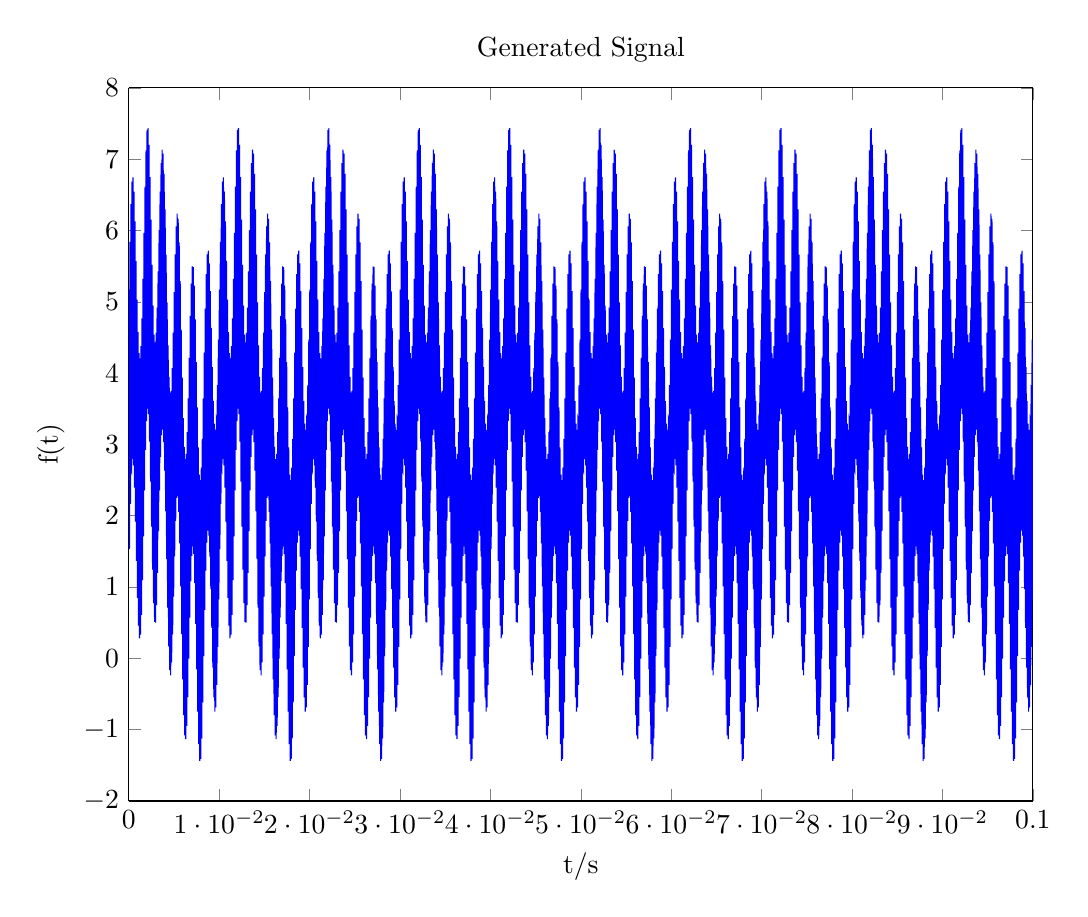
\begin{tikzpicture}

\begin{axis}[%
width=4.520833in,
height=3.565625in,
at={(0.758333in,0.48125in)},
scale only axis,
separate axis lines,
every outer x axis line/.append style={black},
every x tick label/.append style={font=\color{black}},
xmin=0,
xmax=0.1,
xlabel={t/s},
every outer y axis line/.append style={black},
every y tick label/.append style={font=\color{black}},
ymin=-2,
ymax=8,
ylabel={f(t)},
title={Generated Signal}
]
\addplot [color=blue,solid,forget plot]
  table[row sep=crcr]{%
0	3\\
1e-05	4.13447200792845\\
2e-05	4.93521035310729\\
3e-05	5.17236241965459\\
4e-05	4.79149496467605\\
5e-05	3.93051671970661\\
6e-05	2.8767165497643\\
7e-05	1.97729312290989\\
8e-05	1.53123218908794\\
9e-05	1.69619487949\\
0.0001	2.43940684397138\\
0.00011	3.54783864022627\\
0.00012	4.69450780370776\\
0.00013	5.54025986990388\\
0.00014	5.83933945586093\\
0.00015	5.5158824945369\\
0.00016	4.68751424391071\\
0.00017	3.62870599969009\\
0.00018	2.68529921495215\\
0.00019	2.16680947146704\\
0.0002	2.25004085986703\\
0.00021	2.92401989540883\\
0.00022	3.99339349959329\\
0.00023	5.13923313219957\\
0.00024	6.01831408832972\\
0.00025	6.36995995660265\\
0.00026	6.09718686499263\\
0.00027	5.29688375053492\\
0.00028	4.22963222385095\\
0.00029	3.23856245735008\\
0.0003	2.64250886069445\\
0.00031	2.6367309168424\\
0.00032	3.23210918234195\\
0.00033	4.25174743709056\\
0.00034	5.38603889881748\\
0.00035	6.28905197183938\\
0.00036	6.68622640315821\\
0.00037	6.45984928855812\\
0.00038	5.68569848377213\\
0.00039	4.60944471720873\\
0.0004	3.57015947522232\\
0.00041	2.89474403783183\\
0.00042	2.79614857113824\\
0.00043	3.30707016938658\\
0.00044	4.26977257490238\\
0.00045	5.38519714676085\\
0.00046	6.30607466433336\\
0.00047	6.7450481480336\\
0.00048	6.56414328588108\\
0.00049	5.81773036696989\\
0.0005	4.73560176881768\\
0.00051	3.65143371617812\\
0.00052	2.89890531512685\\
0.00053	2.70781758305348\\
0.00054	3.1325551951983\\
0.00055	4.03516395156119\\
0.00056	5.12831268179471\\
0.00057	6.0647636350973\\
0.00058	6.5454952562464\\
0.00059	6.4128139364528\\
0.0006	5.69946492143331\\
0.00061	4.61845196293269\\
0.00062	3.49673528465023\\
0.00063	2.67345059090888\\
0.00064	2.39433801113204\\
0.00065	2.73524988650792\\
0.00066	3.57855277688623\\
0.00067	4.6497707590412\\
0.00068	5.60306131295207\\
0.00069	6.12891135134133\\
0.0007	6.05052283530795\\
0.00071	5.37887884931338\\
0.00072	4.30934560526946\\
0.00073	3.16086829119145\\
0.00074	2.27669174984777\\
0.00075	1.91751599130197\\
0.00076	2.18035191289345\\
0.00077	2.96834099048291\\
0.00078	4.02093537006556\\
0.00079	4.99504193095764\\
0.0008	5.57186655703848\\
0.00081	5.55619324280871\\
0.00082	4.93718803067531\\
0.00083	3.89179679433597\\
0.00084	2.7296789531014\\
0.00085	1.79682164770651\\
0.00086	1.36784350464814\\
0.00087	1.56051854650603\\
0.00088	2.29913269329495\\
0.00089	3.33808155848227\\
0.0009	4.33836246881667\\
0.00091	4.97314533019842\\
0.00092	5.02955343348083\\
0.00093	4.47496530740137\\
0.00094	3.46719489056209\\
0.00095	2.30538045175462\\
0.00096	1.33687267264294\\
0.00097	0.849111710643196\\
0.00098	0.980156653548294\\
0.00099	1.6757234649783\\
0.001	2.70610737385376\\
0.00101	3.73772099048355\\
0.00102	4.4369751456354\\
0.00103	4.57415973213644\\
0.00104	4.0949818285479\\
0.00105	3.13748810127074\\
0.00106	1.98910276765646\\
0.00107	0.997157073294764\\
0.00108	0.460766382527009\\
0.00109	0.537718293693981\\
0.0011	1.19536159691072\\
0.00111	2.22078648832871\\
0.00112	3.28712647012046\\
0.00113	4.05533920803906\\
0.00114	4.27977745367812\\
0.00115	3.88468112524116\\
0.00116	2.98777516896432\\
0.00117	1.86362613024529\\
0.00118	0.858166138013741\\
0.00119	0.280996747285292\\
0.0012	0.309003197245347\\
0.00121	0.931288211783095\\
0.00122	1.95256987290421\\
0.00123	3.05398565173272\\
0.00124	3.89237161184199\\
0.00125	4.20710678118655\\
0.00126	3.90125731925243\\
0.00127	3.07175671576106\\
0.00128	1.97922559197929\\
0.00129	0.966827533582796\\
0.0013	0.353424718738071\\
0.00131	0.334298714785433\\
0.00132	0.920346447250909\\
0.00133	1.93468232644733\\
0.00134	3.06770444695425\\
0.00135	3.97348032954798\\
0.00136	4.37744307866127\\
0.00137	4.16186739802689\\
0.00138	3.40251301956244\\
0.00139	2.34502684196146\\
0.0014	1.32845084993781\\
0.00141	0.679651191979597\\
0.00142	0.611537322803333\\
0.00143	1.15676010338324\\
0.00144	2.15753158670276\\
0.00145	3.31473605999348\\
0.00146	4.28104192950115\\
0.00147	4.76902462998599\\
0.00148	4.64063714744874\\
0.00149	3.9501720560336\\
0.0015	2.92733911593625\\
0.00151	1.90572714974283\\
0.00152	1.2189232008432\\
0.00153	1.09663169437406\\
0.00154	1.59313632114463\\
0.00155	2.57037764817708\\
0.00156	3.74091517326974\\
0.00157	4.75739787038613\\
0.00158	5.3206871267887\\
0.00159	5.27296866036971\\
0.0016	4.64686359933969\\
0.00161	3.65524831026064\\
0.00162	2.62495254512833\\
0.00163	1.8949786355846\\
0.00164	1.71093062706029\\
0.00165	2.14852225896009\\
0.00166	3.08997916865847\\
0.00167	4.26068239016097\\
0.00168	5.31464444379656\\
0.00169	5.9422055718933\\
0.0017	5.96641956298063\\
0.00171	5.39812003748026\\
0.00172	4.43252266433514\\
0.00173	3.38842122373787\\
0.00174	2.6089085010855\\
0.00175	2.35453201575079\\
0.00176	2.72214995790901\\
0.00177	3.6147510969378\\
0.00178	4.77163509018488\\
0.00179	5.84955676300066\\
0.0018	6.52957059620891\\
0.00181	6.61631004747063\\
0.00182	6.09879170264375\\
0.00183	5.15381327170835\\
0.00184	4.09088751379346\\
0.00185	3.25585662155712\\
0.00186	2.92319619166071\\
0.00187	3.2105393385016\\
0.00188	4.0420333959629\\
0.00189	5.17193791052957\\
0.0019	6.26111685463689\\
0.00191	6.98260968220647\\
0.00192	7.12341231998976\\
0.00193	6.65077920165422\\
0.00194	5.72240361627405\\
0.00195	4.63730680027014\\
0.00196	3.74272618656815\\
0.00197	3.32599262857834\\
0.00198	3.52506001031439\\
0.00199	4.2855433415131\\
0.002	5.37764129073788\\
0.00201	6.46767443885433\\
0.00202	7.22196624905069\\
0.00203	7.41072403276416\\
0.00204	6.97957719088074\\
0.00205	6.06649972639853\\
0.00206	4.95884831097111\\
0.00207	4.0038918583562\\
0.00208	3.50068870368162\\
0.00209	3.60697479991089\\
0.0021	4.29005274918611\\
0.00211	5.33697208290346\\
0.00212	6.42083121966311\\
0.00213	7.20255837286366\\
0.00214	7.43648251499541\\
0.00215	7.04682549238159\\
0.00216	6.15129991246361\\
0.00217	5.02446573264614\\
0.00218	4.01225425421178\\
0.00219	3.42427196623488\\
0.0022	3.43741479683741\\
0.00221	4.04080189871827\\
0.00222	5.03917349940489\\
0.00223	6.11369490097119\\
0.00224	6.92123564400564\\
0.00225	7.20121383215756\\
0.00226	6.85674024394685\\
0.00227	5.98479846824993\\
0.00228	4.84606463460527\\
0.00229	3.78376316738602\\
0.0023	3.11682232761719\\
0.00231	3.04059491594198\\
0.00232	3.56605414059867\\
0.00233	4.51639563581181\\
0.00234	5.58210354604083\\
0.00235	6.41733614582149\\
0.00236	6.74762186845336\\
0.00237	6.45533518636976\\
0.00238	5.61633989844045\\
0.00239	4.4763911208731\\
0.0024	3.37464305287035\\
0.00241	2.63807789511695\\
0.00242	2.47972482751419\\
0.00243	2.93235793927014\\
0.00244	3.838315839735\\
0.00245	4.89861252099426\\
0.00246	5.76604905851605\\
0.00247	6.15333633231999\\
0.00248	5.92256535742776\\
0.00249	5.12816912481904\\
0.0025	4\\
0.00251	2.87179139689325\\
0.00252	2.07727673097988\\
0.00253	1.84630837244163\\
0.00254	2.23331932005059\\
0.00255	3.10040059973725\\
0.00256	4.16026310554623\\
0.00257	5.0657079300861\\
0.00258	5.51774908569784\\
0.00259	5.35872520510099\\
0.0026	4.6214104039862\\
0.00261	3.51883389184935\\
0.00262	2.37797790208078\\
0.00263	1.53799666969827\\
0.00264	1.24464534983299\\
0.00265	1.57378778338469\\
0.00266	2.40779848792182\\
0.00267	3.47220594498218\\
0.00268	4.42116848044134\\
0.00269	4.94517029319764\\
0.0027	4.86740707501175\\
0.00271	4.19885209475295\\
0.00272	3.13485821678799\\
0.00273	1.99435376895532\\
0.00274	1.12056324552895\\
0.00275	0.774162849032717\\
0.00276	1.05213624441013\\
0.00277	1.85759428932683\\
0.00278	2.92995516965354\\
0.00279	3.9260885112724\\
0.0028	4.52715970461997\\
0.00281	4.53790906865179\\
0.00282	3.94745585055674\\
0.00283	2.93269607600484\\
0.00284	1.80323633467276\\
0.00285	0.905008031495895\\
0.00286	0.512571230577743\\
0.00287	0.743638649100601\\
0.00288	1.52243224616628\\
0.00289	2.6032811100768\\
0.0029	3.64711357307119\\
0.00291	4.327028175614\\
0.00292	4.43007457398492\\
0.00293	3.92355549822379\\
0.00294	2.96520703220101\\
0.00295	1.85408764495531\\
0.00296	0.937466387153979\\
0.00297	0.502700070353502\\
0.00298	0.687762840442605\\
0.00299	1.43828424418007\\
0.003	2.5244717418524\\
0.00301	3.61264894846745\\
0.00302	4.36913659967509\\
0.00303	4.56413352178127\\
0.00304	4.14325488521753\\
0.00305	3.24445473763829\\
0.00306	2.15506409903365\\
0.00307	1.22232057184213\\
0.00308	0.745245564923453\\
0.00309	0.881532542709968\\
0.0031	1.59843611713965\\
0.00311	2.6829523961398\\
0.00312	3.80812101770606\\
0.00313	4.63480614123865\\
0.00314	4.91726750307104\\
0.00315	4.57965262981082\\
0.00316	3.73959483144838\\
0.00317	2.67156990309867\\
0.00318	1.72142023872623\\
0.00319	1.1986588016116\\
0.0032	1.28008350872314\\
0.00321	1.95471115573576\\
0.00322	3.02717541294783\\
0.00323	4.17853097663272\\
0.00324	5.06553289039354\\
0.00325	5.42748103262595\\
0.00326	5.16736439654156\\
0.00327	4.38204139892697\\
0.00328	3.33205978853469\\
0.00329	2.36051258290082\\
0.0033	1.78619379710709\\
0.00331	1.80431933772654\\
0.00332	2.42572306554249\\
0.00333	3.47345901216801\\
0.00334	4.63786766572719\\
0.00335	5.57296179504781\\
0.00336	6.00412268532702\\
0.00337	5.81357622781398\\
0.00338	5.07703641846104\\
0.00339	4.04010756190954\\
0.0034	3.04179225166435\\
0.00341	2.40892050422663\\
0.00342	2.35436895329558\\
0.00343	2.91075899684027\\
0.00344	3.92027662512196\\
0.00345	5.08378350037212\\
0.00346	6.05392887411228\\
0.00347	6.54327252427685\\
0.00348	6.41375530059117\\
0.00349	5.71966117912337\\
0.0035	4.69069487281365\\
0.00351	3.66044371538862\\
0.00352	2.962496822293\\
0.00353	2.82656424909115\\
0.00354	3.30693886779454\\
0.00355	4.26557396475792\\
0.00356	5.41504527757044\\
0.00357	6.40802151776995\\
0.00358	6.94538728033073\\
0.00359	6.86935492841787\\
0.0036	6.2125756356137\\
0.00361	5.18795917165722\\
0.00362	4.12237200246039\\
0.00363	3.35485643255055\\
0.00364	3.13105968281094\\
0.00365	3.52674180971295\\
0.00366	4.42417784389414\\
0.00367	5.54880121903017\\
0.00368	6.55467978746547\\
0.00369	7.13221197765969\\
0.0037	7.10451253610475\\
0.00371	6.48247872679133\\
0.00372	5.46139245779651\\
0.00373	4.36011625028264\\
0.00374	3.52181403516613\\
0.00375	3.20710678118655\\
0.00376	3.51292832775572\\
0.00377	4.34234518625422\\
0.00378	5.43473673872145\\
0.00379	6.44693940499166\\
0.0038	7.06009101461204\\
0.00381	7.07891001015953\\
0.00382	6.49249947822829\\
0.00383	5.47774502282805\\
0.00384	4.34424856590416\\
0.00385	3.43794260540615\\
0.00386	3.03339405782779\\
0.00387	3.2483282425627\\
0.00388	4.00698545301847\\
0.00389	5.0637188180245\\
0.0039	6.07948638258664\\
0.00391	6.72742203013228\\
0.00392	6.79461634005437\\
0.00393	6.24841848768145\\
0.00394	5.24661645852422\\
0.00395	4.08832600603516\\
0.00396	3.12087876684132\\
0.00397	2.6316993512416\\
0.00398	2.75883482047964\\
0.00399	3.4479926498386\\
0.004	4.46946313073117\\
0.00401	5.48965749435888\\
0.00402	6.17498875329625\\
0.00403	6.29575254054598\\
0.00404	5.79766522561058\\
0.00405	4.81878630394959\\
0.00406	3.6465563424143\\
0.00407	2.62832643385541\\
0.00408	2.0632352599877\\
0.00409	2.10909717405537\\
0.0041	2.73329112114137\\
0.00411	3.72294081013118\\
0.00412	4.75121656662768\\
0.00413	5.47911613873539\\
0.00414	5.66103556291487\\
0.00415	5.22126118379424\\
0.00416	4.27756745017007\\
0.00417	3.10457341634302\\
0.00418	2.04826665242122\\
0.00419	1.41830700864195\\
0.0042	1.39164079116496\\
0.00421	1.95743447637823\\
0.00422	2.92047249426516\\
0.00423	3.96196116567201\\
0.00424	4.73880780834956\\
0.00425	4.99046500817712\\
0.00426	4.62007468233228\\
0.00427	3.72464817088634\\
0.00428	2.56488592803245\\
0.00429	1.48403324204848\\
0.0043	0.801035747822192\\
0.00431	0.711260105482297\\
0.00432	1.22568984903451\\
0.00433	2.16752739043156\\
0.00434	3.22726009454111\\
0.00435	4.05904589476167\\
0.00436	4.38840932254237\\
0.00437	4.09771739364588\\
0.00438	3.26282290639337\\
0.00439	2.12946644854283\\
0.0044	1.03678418393604\\
0.00441	0.311736796956263\\
0.00442	0.167328501180099\\
0.00443	0.636305005285229\\
0.00444	1.56097316455434\\
0.00445	2.64231188892935\\
0.00446	3.53308389384768\\
0.00447	3.9459584762564\\
0.00448	3.74298190448753\\
0.00449	2.97853932313248\\
0.0045	1.88243221993214\\
0.00451	0.788340172295638\\
0.00452	0.0299398772729527\\
0.00453	-0.162975814377045\\
0.00454	0.263963860606643\\
0.00455	1.17278506531758\\
0.00456	2.27613129613235\\
0.00457	3.22673380925415\\
0.00458	3.72553444144156\\
0.00459	3.61479741353495\\
0.0046	2.92722029910733\\
0.00461	1.87575374438212\\
0.00462	0.787299510275346\\
0.00463	0.000929564795071336\\
0.00464	-0.237684881259455\\
0.00465	0.147234510953684\\
0.00466	1.03797532102661\\
0.00467	2.1599777804493\\
0.00468	3.16731077868693\\
0.00469	3.75036801925934\\
0.0047	3.73225376847698\\
0.00471	3.12384906990414\\
0.00472	2.12041389409962\\
0.00473	1.04078313889047\\
0.00474	0.228087465397148\\
0.00475	-0.0570910265221896\\
0.00476	0.282137089911788\\
0.00477	1.14878843290502\\
0.00478	2.28218708177596\\
0.00479	3.33910882277572\\
0.0048	4.00062560726157\\
0.00481	4.0713848487227\\
0.00482	3.54041355479483\\
0.00483	2.58451630886045\\
0.00484	1.51320918579174\\
0.00485	0.672334132100134\\
0.00486	0.33636293724056\\
0.00487	0.622921353232425\\
0.00488	1.45614580734819\\
0.00489	2.59028141120264\\
0.0049	3.68617419508732\\
0.00491	4.41684218947404\\
0.00492	4.56925644727158\\
0.00493	4.11064311372585\\
0.00494	3.19866381557548\\
0.00495	2.13230479844966\\
0.00496	1.25876522621063\\
0.00497	0.86533445977623\\
0.00498	1.08992172665941\\
0.00499	1.87809428000266\\
0.005	2.99999999999999\\
0.00501	4.12190571999733\\
0.00502	4.91007827334058\\
0.00503	5.13466554022377\\
0.00504	4.74123477378938\\
0.00505	3.86769520155036\\
0.00506	2.80133618442443\\
0.00507	1.88935688627408\\
0.00508	1.4307435527284\\
0.00509	1.58315781052599\\
0.0051	2.31382580491276\\
0.00511	3.40971858879758\\
0.00512	4.5438541926519\\
0.00513	5.37707864676756\\
0.00514	5.66363706275944\\
0.00515	5.32766586789987\\
0.00516	4.48679081420827\\
0.00517	3.41548369113956\\
0.00518	2.45958644520519\\
0.00519	1.9286151512773\\
0.0052	1.99937439273843\\
0.00521	2.66089117722427\\
0.00522	3.71781291822403\\
0.00523	4.85121156709507\\
0.00524	5.71786291008821\\
0.00525	6.05709102652219\\
0.00526	5.7719125346028\\
0.00527	4.95921686110944\\
0.00528	3.87958610590028\\
0.00529	2.87615093009579\\
0.0053	2.26774623152299\\
0.00531	2.24963198074069\\
0.00532	2.83268922131314\\
0.00533	3.8400222195508\\
0.00534	4.96202467897338\\
0.00535	5.85276548904631\\
0.00536	6.23768488125945\\
0.00537	5.99907043520494\\
0.00538	5.21270048972467\\
0.00539	4.1242462556179\\
0.0054	3.07277970089259\\
0.00541	2.38520258646506\\
0.00542	2.27446555855845\\
0.00543	2.77326619074584\\
0.00544	3.72386870386774\\
0.00545	4.8272149346824\\
0.00546	5.73603613939342\\
0.00547	6.16297581437704\\
0.00548	5.970060122727\\
0.00549	5.21165982770433\\
0.0055	4.11756778006776\\
0.00551	3.02146067686749\\
0.00552	2.25701809551243\\
0.00553	2.0540415237436\\
0.00554	2.46691610615235\\
0.00555	3.35768811107064\\
0.00556	4.4390268354457\\
0.00557	5.3636949947148\\
0.00558	5.83267149881991\\
0.00559	5.6882632030437\\
0.0056	4.96321581606392\\
0.00561	3.87053355145707\\
0.00562	2.7371770936066\\
0.00563	1.90228260635407\\
0.00564	1.61159067745763\\
0.00565	1.94095410523838\\
0.00566	2.77273990545882\\
0.00567	3.83247260956854\\
0.00568	4.77431015096552\\
0.00569	5.28873989451772\\
0.0057	5.1989642521778\\
0.00571	4.51596675795143\\
0.00572	3.43511407196757\\
0.00573	2.27535182911361\\
0.00574	1.37992531766769\\
0.00575	1.00953499182287\\
0.00576	1.26119219165049\\
0.00577	2.03803883432802\\
0.00578	3.07952750573493\\
0.00579	4.0425655236218\\
0.0058	4.60835920883506\\
0.00581	4.58169299135806\\
0.00582	3.9517333475787\\
0.00583	2.89542658365705\\
0.00584	1.72243254982983\\
0.00585	0.778738816205799\\
0.00586	0.338964437085119\\
0.00587	0.520883861264629\\
0.00588	1.2487834333724\\
0.00589	2.27705918986886\\
0.0059	3.26670887885871\\
0.00591	3.89090282594468\\
0.00592	3.93676474001228\\
0.00593	3.37167356614448\\
0.00594	2.35344365758566\\
0.00595	1.18121369605031\\
0.00596	0.202334774389395\\
0.00597	-0.295752540545995\\
0.00598	-0.174988753296274\\
0.00599	0.510342505641196\\
0.006	1.53053686926876\\
0.00601	2.55200735016148\\
0.00602	3.24116517952033\\
0.00603	3.36830064875838\\
0.00604	2.87912123315873\\
0.00605	1.91167399396474\\
0.00606	0.75338354147585\\
0.00607	-0.248418487681515\\
0.00608	-0.794616340054406\\
0.00609	-0.727422030132247\\
0.0061	-0.0794863825866061\\
0.00611	0.9362811819756\\
0.00612	1.99301454698162\\
0.00613	2.75167175743732\\
0.00614	2.9666059421722\\
0.00615	2.56205739459389\\
0.00616	1.65575143409574\\
0.00617	0.52225497717191\\
0.00618	-0.492499478228364\\
0.00619	-1.07891001015954\\
0.0062	-1.06009101461201\\
0.00621	-0.44693940499163\\
0.00622	0.565263261278646\\
0.00623	1.65765481374572\\
0.00624	2.48707167224434\\
0.00625	2.79289321881345\\
0.00626	2.47818596483382\\
0.00627	1.63988374971732\\
0.00628	0.538607542203395\\
0.00629	-0.482478726791357\\
0.0063	-1.10451253610478\\
0.00631	-1.13221197765967\\
0.00632	-0.554679787465485\\
0.00633	0.451198780969928\\
0.00634	1.57582215610585\\
0.00635	2.47325819028711\\
0.00636	2.86894031718906\\
0.00637	2.64514356744941\\
0.00638	1.87762799753958\\
0.00639	0.812040828342688\\
0.0064	-0.212575635613734\\
0.00641	-0.869354928417907\\
0.00642	-0.945387280330721\\
0.00643	-0.408021517769964\\
0.00644	0.584954722429494\\
0.00645	1.73442603524218\\
0.00646	2.69306113220553\\
0.00647	3.17343575090886\\
0.00648	3.03750317770696\\
0.00649	2.33955628461139\\
0.0065	1.30930512718625\\
0.00651	0.280338820876649\\
0.00652	-0.413755300591204\\
0.00653	-0.543272524276849\\
0.00654	-0.0539288741121768\\
0.00655	0.916216499627919\\
0.00656	2.07972337487819\\
0.00657	3.08924100315977\\
0.00658	3.64563104670444\\
0.00659	3.59107949577337\\
0.0066	2.95820774833557\\
0.00661	1.95989243809048\\
0.00662	0.922963581538979\\
0.00663	0.186423772186028\\
0.00664	-0.00412268532701621\\
0.00665	0.427038204952184\\
0.00666	1.36213233427279\\
0.00667	2.52654098783209\\
0.00668	3.5742769344575\\
0.00669	4.19568066227348\\
0.0067	4.21380620289291\\
0.00671	3.63948741709907\\
0.00672	2.66794021146527\\
0.00673	1.61795860107289\\
0.00674	0.832635603458421\\
0.00675	0.57251896737406\\
0.00676	0.934467109606477\\
0.00677	1.82146902336742\\
0.00678	2.97282458705216\\
0.00679	4.04528884426423\\
0.0068	4.71991649127686\\
0.00681	4.80134119838841\\
0.00682	4.27857976127379\\
0.00683	3.32843009690135\\
0.00684	2.26040516855163\\
0.00685	1.42034737018916\\
0.00686	1.08273249692896\\
0.00687	1.36519385876136\\
0.00688	2.19187898229407\\
0.00689	3.31704760386024\\
0.0069	4.40156388286048\\
0.00691	5.11846745729005\\
0.00692	5.25475443507652\\
0.00693	4.77767942815784\\
0.00694	3.8449359009662\\
0.00695	2.75554526236167\\
0.00696	1.85674511478245\\
0.00697	1.43586647821873\\
0.00698	1.63086340032491\\
0.00699	2.38735105153253\\
0.007	3.47552825814759\\
0.00701	4.56171575581991\\
0.00702	5.31223715955741\\
0.00703	5.49729992964649\\
0.00704	5.062533612846\\
0.00705	4.14591235504465\\
0.00706	3.03479296779895\\
0.00707	2.0764445017761\\
0.00708	1.56992542601507\\
0.00709	1.67297182438606\\
0.0071	2.35288642692884\\
0.00711	3.39671888992335\\
0.00712	4.47756775383365\\
0.00713	5.25636135089942\\
0.00714	5.48742876942225\\
0.00715	5.09499196850408\\
0.00716	4.1967636653271\\
0.00717	3.06730392399517\\
0.00718	2.05254414944327\\
0.00719	1.4620909313482\\
0.0072	1.47284029538008\\
0.00721	2.07391148872763\\
0.00722	3.0700448303465\\
0.00723	4.14240571067321\\
0.00724	4.94786375558996\\
0.00725	5.22583715096728\\
0.00726	4.87943675447102\\
0.00727	4.00564623104464\\
0.00728	2.86514178321186\\
0.00729	1.8011479052471\\
0.0073	1.13259292498823\\
0.00731	1.05482970680237\\
0.00732	1.57883151955869\\
0.00733	2.52779405501775\\
0.00734	3.59220151207823\\
0.00735	4.42621221661533\\
0.00736	4.75535465016701\\
0.00737	4.46200333030162\\
0.00738	3.62202209791919\\
0.00739	2.4811661081506\\
0.0074	1.37858959601377\\
0.00741	0.641274794898942\\
0.00742	0.482250914302144\\
0.00743	0.934292069913924\\
0.00744	1.83973689445381\\
0.00745	2.89959940026289\\
0.00746	3.76668067994937\\
0.00747	4.15369162755838\\
0.00748	3.9227232690201\\
0.00749	3.12820860310662\\
0.0075	2.00000000000007\\
0.00751	0.871830875180929\\
0.00752	0.0774346425722241\\
0.00753	-0.153336332319994\\
0.00754	0.233950941483944\\
0.00755	1.10138747900583\\
0.00756	2.16168416026509\\
0.00757	3.06764206072989\\
0.00758	3.52027517248584\\
0.00759	3.36192210488303\\
0.0076	2.62535694712962\\
0.00761	1.52360887912686\\
0.00762	0.383660101559402\\
0.00763	-0.455335186369727\\
0.00764	-0.747621868453356\\
0.00765	-0.417336145821441\\
0.00766	0.417896453959362\\
0.00767	1.48360436418811\\
0.00768	2.43394585940136\\
0.00769	2.95940508405802\\
0.0077	2.88317767238282\\
0.00771	2.21623683261399\\
0.00772	1.15393536539463\\
0.00773	0.0152015317499723\\
0.00774	-0.856740243946843\\
0.00775	-1.20121383215756\\
0.00776	-0.921235644005585\\
0.00777	-0.113694900971127\\
0.00778	0.960826500595177\\
0.00779	1.95919810128187\\
0.0078	2.56258520316257\\
0.00781	2.5757280337651\\
0.00782	1.98774574578816\\
0.00783	0.975534267353907\\
0.00784	-0.151299912463783\\
0.00785	-1.04682549238163\\
0.00786	-1.43648251499542\\
0.00787	-1.20255837286368\\
0.00788	-0.420831219663119\\
0.00789	0.663027917096641\\
0.0079	1.70994725081397\\
0.00791	2.3930252000891\\
0.00792	2.49931129631839\\
0.00793	1.99610814164374\\
0.00794	1.04115168902879\\
0.00795	-0.0664997263985172\\
0.00796	-0.979577190880732\\
0.00797	-1.41072403276418\\
0.00798	-1.22196624905066\\
0.00799	-0.467674438854274\\
0.008	0.62235870926208\\
0.00801	1.71445665848705\\
0.00802	2.47493998968564\\
0.00803	2.67400737142165\\
0.00804	2.25727381343184\\
0.00805	1.3626931997299\\
0.00806	0.277596383725858\\
0.00807	-0.650779201654282\\
0.00808	-1.12341231998976\\
0.00809	-0.982609682206478\\
0.0081	-0.261116854636805\\
0.00811	0.828062089470526\\
0.00812	1.95796660403709\\
0.00813	2.78946066149839\\
0.00814	3.07680380833929\\
0.00815	2.74414337844283\\
0.00816	1.90911248620645\\
0.00817	0.846186728291668\\
0.00818	-0.0987917026439171\\
0.00819	-0.616310047470656\\
0.0082	-0.529570596208865\\
0.00821	0.150443236999352\\
0.00822	1.22836490981507\\
0.00823	2.3852489030623\\
0.00824	3.27785004209105\\
0.00825	3.64546798424921\\
0.00826	3.39109149891451\\
0.00827	2.61157877626202\\
0.00828	1.56747733566474\\
0.00829	0.601879962519749\\
0.0083	0.0335804370193822\\
0.00831	0.057794428106706\\
0.00832	0.685355556203524\\
0.00833	1.73931760983902\\
0.00834	2.91002083134152\\
0.00835	3.85147774104005\\
0.00836	4.28906937293972\\
0.00837	4.10502136441534\\
0.00838	3.37504745487166\\
0.00839	2.34475168973938\\
0.0084	1.35313640066024\\
0.00841	0.727031339630257\\
0.00842	0.679312873211299\\
0.00843	1.24260212961387\\
0.00844	2.25908482673039\\
0.00845	3.42962235182304\\
0.00846	4.40686367885538\\
0.00847	4.90336830562594\\
0.00848	4.78107679915676\\
0.00849	4.09427285025708\\
0.0085	3.07266088406377\\
0.00851	2.04982794396639\\
0.00852	1.35936285255126\\
0.00853	1.23097537001403\\
0.00854	1.71895807049886\\
0.00855	2.68526394000653\\
0.00856	3.84246841329714\\
0.00857	4.84323989661685\\
0.00858	5.3884626771967\\
0.00859	5.3203488080204\\
0.0086	4.67154915006218\\
0.00861	3.65497315803841\\
0.00862	2.59748698043745\\
0.00863	1.8381326019731\\
0.00864	1.62255692133873\\
0.00865	2.0265196704521\\
0.00866	2.93229555304587\\
0.00867	4.06531767355268\\
0.00868	5.07965355274912\\
0.00869	5.66570128521457\\
0.0087	5.64657528126189\\
0.00871	5.0331724664172\\
0.00872	4.0207744080207\\
0.00873	2.92824328423904\\
0.00874	2.0987426807475\\
0.00875	1.79289321881345\\
0.00876	2.10762838815801\\
0.00877	2.94601434826732\\
0.00878	4.04743012709595\\
0.00879	5.068711788217\\
0.0088	5.69099680275466\\
0.00881	5.7190032527147\\
0.00882	5.14183386198616\\
0.00883	4.13637386975456\\
0.00884	3.01222483103567\\
0.00885	2.11531887475882\\
0.00886	1.72022254632187\\
0.00887	1.94466079196101\\
0.00888	2.71287352987958\\
0.00889	3.77921351167132\\
0.0089	4.80463840308921\\
0.00891	5.46228170630607\\
0.00892	5.53923361747298\\
0.00893	5.00284292670523\\
0.00894	4.01089723234362\\
0.00895	2.86251189872911\\
0.00896	1.905018171452\\
0.00897	1.42584026786355\\
0.00898	1.56302485436463\\
0.00899	2.26227900951656\\
0.009	3.29389262614638\\
0.00901	4.32427653502172\\
0.00902	5.01984334645173\\
0.00903	5.15088828935679\\
0.00904	4.66312732735696\\
0.00905	3.69461954824534\\
0.00906	2.53280510943776\\
0.00907	1.52503469259868\\
0.00908	0.970446566519139\\
0.00909	1.02685466980155\\
0.0091	1.66163753118328\\
0.00911	2.66191844151764\\
0.00912	3.70086730670518\\
0.00913	4.43948145349393\\
0.00914	4.63215649535186\\
0.00915	4.20317835229354\\
0.00916	3.27032104689845\\
0.00917	2.10820320566388\\
0.00918	1.06281196932473\\
0.00919	0.443806757191257\\
0.0092	0.428133442961558\\
0.00921	1.00495806904247\\
0.00922	1.97906462993439\\
0.00923	3.03165900951724\\
0.00924	3.81964808710652\\
0.00925	4.08248400869803\\
0.00926	3.72330825015226\\
0.00927	2.8391317088086\\
0.00928	1.6906543947306\\
0.00929	0.621121150686485\\
0.0093	-0.0505228353079419\\
0.00931	-0.12891135134134\\
0.00932	0.396938687047888\\
0.00933	1.35022924095896\\
0.00934	2.42144722311394\\
0.00935	3.26475011349204\\
0.00936	3.60566198886797\\
0.00937	3.32654940909104\\
0.00938	2.50326471534962\\
0.00939	1.38154803706736\\
0.0094	0.300535078566549\\
0.00941	-0.412813936452777\\
0.00942	-0.545495256246377\\
0.00943	-0.0647636350973348\\
0.00944	0.871687318205242\\
0.00945	1.96483604843876\\
0.00946	2.86744480480181\\
0.00947	3.29218241694651\\
0.00948	3.10109468487316\\
0.00949	2.34856628382192\\
0.0095	1.26439823118214\\
0.00951	0.182269633030145\\
0.00952	-0.564143285881066\\
0.00953	-0.745048148033602\\
0.00954	-0.306074664333242\\
0.00955	0.614802853239332\\
0.00956	1.73022742509758\\
0.00957	2.69292983061355\\
0.00958	3.20385142886175\\
0.00959	3.1052559621681\\
0.0096	2.42984052477772\\
0.00961	1.39055528279131\\
0.00962	0.314301516227904\\
0.00963	-0.459849288558215\\
0.00964	-0.686226403158215\\
0.00965	-0.289051971839409\\
0.00966	0.61396110118249\\
0.00967	1.74825256290964\\
0.00968	2.76789081765803\\
0.00969	3.36326908315759\\
0.0097	3.35749113930556\\
0.00971	2.76143754264979\\
0.00972	1.77036777614908\\
0.00973	0.703116249465112\\
0.00974	-0.0971868649926124\\
0.00975	-0.369959956602658\\
0.00976	-0.018314088329606\\
0.00977	0.860766867800399\\
0.00978	2.00660650040691\\
0.00979	3.07598010459114\\
0.0098	3.74995914013303\\
0.00981	3.83319052853297\\
0.00982	3.31470078504786\\
0.00983	2.37129400030993\\
0.00984	1.31248575608911\\
0.00985	0.484117505463118\\
0.00986	0.160660544139079\\
0.00987	0.459740130096105\\
0.00988	1.30549219629242\\
0.00989	2.45216135977371\\
0.0099	3.5605931560286\\
0.00991	4.30380512051\\
0.00992	4.46876781091205\\
0.00993	4.02270687708998\\
0.00994	3.12328345023572\\
0.00995	2.0694832802932\\
0.00996	1.20850503532396\\
0.00997	0.827637580345395\\
0.00998	1.06478964689271\\
0.00999	1.86552799207153\\
0.01	2.99999999999998\\
0.01001	4.13447200792864\\
0.01002	4.93521035310729\\
0.01003	5.1723624196546\\
0.01004	4.79149496467605\\
0.01005	3.93051671970642\\
0.01006	2.87671654976431\\
0.01007	1.9772931229099\\
0.01008	1.53123218908795\\
0.01009	1.69619487949\\
0.0101	2.43940684397138\\
0.01011	3.54783864022627\\
0.01012	4.69450780370775\\
0.01013	5.54025986990388\\
0.01014	5.83933945586092\\
0.01015	5.51588249453691\\
0.01016	4.68751424391071\\
0.01017	3.6287059996901\\
0.01018	2.68529921495199\\
0.01019	2.16680947146705\\
0.0102	2.25004085986703\\
0.01021	2.92401989540883\\
0.01022	3.99339349959352\\
0.01023	5.13923313219957\\
0.01024	6.01831408832972\\
0.01025	6.36995995660266\\
0.01026	6.09718686499263\\
0.01027	5.29688375053492\\
0.01028	4.22963222385095\\
0.01029	3.23856245735007\\
0.0103	2.64250886069444\\
0.01031	2.63673091684241\\
0.01032	3.23210918234195\\
0.01033	4.25174743709056\\
0.01034	5.38603889881748\\
0.01035	6.28905197183952\\
0.01036	6.68622640315822\\
0.01037	6.45984928855812\\
0.01038	5.68569848377212\\
0.01039	4.6094447172085\\
0.0104	3.57015947522231\\
0.01041	2.89474403783183\\
0.01042	2.79614857113825\\
0.01043	3.30707016938659\\
0.01044	4.26977257490239\\
0.01045	5.38519714676086\\
0.01046	6.30607466433337\\
0.01047	6.7450481480336\\
0.01048	6.56414328588107\\
0.01049	5.81773036696988\\
0.0105	4.73560176881766\\
0.01051	3.65143371617811\\
0.01052	2.89890531512675\\
0.01053	2.70781758305348\\
0.01054	3.13255519519832\\
0.01055	4.03516395156121\\
0.01056	5.12831268179494\\
0.01057	6.06476363509731\\
0.01058	6.5454952562464\\
0.01059	6.41281393645279\\
0.0106	5.69946492143329\\
0.01061	4.61845196293267\\
0.01062	3.49673528465021\\
0.01063	2.67345059090886\\
0.01064	2.39433801113204\\
0.01065	2.73524988650793\\
0.01066	3.57855277688624\\
0.01067	4.64977075904123\\
0.01068	5.60306131295208\\
0.01069	6.12891135134134\\
0.0107	6.05052283530794\\
0.01071	5.37887884931336\\
0.01072	4.30934560526944\\
0.01073	3.16086829119122\\
0.01074	2.27669174984776\\
0.01075	1.91751599130197\\
0.01076	2.18035191289347\\
0.01077	2.96834099048294\\
0.01078	4.02093537006558\\
0.01079	4.99504193095768\\
0.0108	5.57186655703849\\
0.01081	5.5561932428087\\
0.01082	4.93718803067529\\
0.01083	3.89179679433593\\
0.01084	2.72967895310136\\
0.01085	1.79682164770648\\
0.01086	1.36784350464813\\
0.01087	1.56051854650604\\
0.01088	2.29913269329499\\
0.01089	3.33808155848233\\
0.0109	4.33836246881669\\
0.01091	4.97314533019842\\
0.01092	5.02955343348082\\
0.01093	4.47496530740134\\
0.01094	3.46719489056227\\
0.01095	2.30538045175458\\
0.01096	1.33687267264292\\
0.01097	0.849111710643185\\
0.01098	0.980156653548312\\
0.01099	1.67572346497833\\
0.011	2.70610737385382\\
0.01101	3.73772099048359\\
0.01102	4.43697514563541\\
0.01103	4.57415973213643\\
0.01104	4.09498182854787\\
0.01105	3.1374881012707\\
0.01106	1.98910276765642\\
0.01107	0.997157073294714\\
0.01108	0.460766382526997\\
0.01109	0.537718293693996\\
0.0111	1.19536159691077\\
0.01111	2.22078648832853\\
0.01112	3.2871264701205\\
0.01113	4.05533920803908\\
0.01114	4.27977745367812\\
0.01115	3.88468112524113\\
0.01116	2.98777516896425\\
0.01117	1.86362613024525\\
0.01118	0.858166138013691\\
0.01119	0.280996747285274\\
0.0112	0.309003197245369\\
0.01121	0.931288211783148\\
0.01122	1.95256987290425\\
0.01123	3.05398565173276\\
0.01124	3.89237161184203\\
0.01125	4.20710678118655\\
0.01126	3.9012573192524\\
0.01127	3.07175671576099\\
0.01128	1.97922559197944\\
0.01129	0.966827533582743\\
0.0113	0.353424718738049\\
0.01131	0.334298714785451\\
0.01132	0.920346447250771\\
0.01133	1.9346823264474\\
0.01134	3.06770444695431\\
0.01135	3.97348032954802\\
0.01136	4.37744307866128\\
0.01137	4.16186739802686\\
0.01138	3.40251301956239\\
0.01139	2.34502684196139\\
0.0114	1.32845084993776\\
0.01141	0.679651191979564\\
0.01142	0.611537322803352\\
0.01143	1.15676010338329\\
0.01144	2.15753158670283\\
0.01145	3.31473605999333\\
0.01146	4.2810419295012\\
0.01147	4.769024629986\\
0.01148	4.64063714744872\\
0.01149	3.95017205603373\\
0.0115	2.92733911593616\\
0.01151	1.90572714974275\\
0.01152	1.21892320084317\\
0.01153	1.09663169437404\\
0.01154	1.59313632114468\\
0.01155	2.57037764817715\\
0.01156	3.74091517326981\\
0.01157	4.75739787038618\\
0.01158	5.32068712678873\\
0.01159	5.27296866036968\\
0.0116	4.64686359933962\\
0.01161	3.65524831026053\\
0.01162	2.62495254512847\\
0.01163	1.89497863558457\\
0.01164	1.7109306270603\\
0.01165	2.14852225896014\\
0.01166	3.08997916865835\\
0.01167	4.26068239016107\\
0.01168	5.31464444379663\\
0.01169	5.94220557189332\\
0.0117	5.96641956298067\\
0.01171	5.39812003748019\\
0.01172	4.43252266433509\\
0.01173	3.3884212237378\\
0.01174	2.60890850108545\\
0.01175	2.35453201575079\\
0.01176	2.72214995790907\\
0.01177	3.61475109693789\\
0.01178	4.77163509018501\\
0.01179	5.84955676300053\\
0.0118	6.52957059620894\\
0.01181	6.61631004747061\\
0.01182	6.09879170264371\\
0.01183	5.15381327170847\\
0.01184	4.09088751379338\\
0.01185	3.25585662155706\\
0.01186	2.9231961916607\\
0.01187	3.21053933850154\\
0.01188	4.04203339596299\\
0.01189	5.17193791052967\\
0.0119	6.26111685463697\\
0.01191	6.98260968220642\\
0.01192	7.12341231998975\\
0.01193	6.65077920165416\\
0.01194	5.72240361627396\\
0.01195	4.63730680027001\\
0.01196	3.74272618656825\\
0.01197	3.32599262857833\\
0.01198	3.52506001031444\\
0.01199	4.28554334151321\\
0.012	5.37764129073777\\
0.01201	6.46767443885444\\
0.01202	7.22196624905074\\
0.01203	7.41072403276414\\
0.01204	6.97957719088082\\
0.01205	6.06649972639844\\
0.01206	4.95884831097102\\
0.01207	4.00389185835613\\
0.01208	3.50068870368164\\
0.01209	3.60697479991093\\
0.0121	4.29005274918619\\
0.01211	5.33697208290355\\
0.01212	6.42083121966299\\
0.01213	7.20255837286361\\
0.01214	7.4364825149954\\
0.01215	7.04682549238151\\
0.01216	6.15129991246349\\
0.01217	5.02446573264624\\
0.01218	4.01225425421169\\
0.01219	3.42427196623484\\
0.0122	3.43741479683745\\
0.01221	4.04080189871819\\
0.01222	5.03917349940501\\
0.01223	6.1136949009713\\
0.01224	6.92123564400569\\
0.01225	7.20121383215756\\
0.01226	6.8567402439468\\
0.01227	5.98479846824984\\
0.01228	4.84606463460517\\
0.01229	3.78376316738612\\
0.0123	3.11682232761723\\
0.01231	3.04059491594202\\
0.01232	3.56605414059878\\
0.01233	4.51639563581197\\
0.01234	5.58210354604071\\
0.01235	6.41733614582155\\
0.01236	6.74762186845337\\
0.01237	6.45533518636968\\
0.01238	5.61633989844053\\
0.01239	4.47639112087294\\
0.0124	3.37464305287022\\
0.01241	2.6380778951169\\
0.01242	2.47972482751418\\
0.01243	2.93235793927024\\
0.01244	3.83831583973509\\
0.01245	4.89861252099436\\
0.01246	5.76604905851597\\
0.01247	6.15333633231997\\
0.01248	5.92256535742768\\
0.01249	5.1281691248189\\
0.0125	4.00000000000008\\
0.01251	2.87179139689331\\
0.01252	2.07727673097981\\
0.01253	1.84630837244165\\
0.01254	2.23331932005067\\
0.01255	3.10040059973718\\
0.01256	4.16026310554636\\
0.01257	5.06570793008621\\
0.01258	5.51774908569787\\
0.01259	5.35872520510102\\
0.0126	4.62141040398606\\
0.01261	3.51883389184919\\
0.01262	2.37797790208064\\
0.01263	1.53799666969834\\
0.01264	1.24464534983298\\
0.01265	1.57378778338478\\
0.01266	2.40779848792195\\
0.01267	3.47220594498211\\
0.01268	4.42116848044129\\
0.01269	4.94517029319763\\
0.0127	4.8674070750117\\
0.01271	4.198852094753\\
0.01272	3.13485821678806\\
0.01273	1.99435376895518\\
0.01274	1.12056324552886\\
0.01275	0.774162849032717\\
0.01276	1.05213624441008\\
0.01277	1.85759428932697\\
0.01278	2.92995516965369\\
0.01279	3.92608851127252\\
0.0128	4.52715970461995\\
0.01281	4.53790906865181\\
0.01282	3.94745585055658\\
0.01283	2.93269607600463\\
0.01284	1.80323633467282\\
0.01285	0.905008031495938\\
0.01286	0.512571230577746\\
0.01287	0.743638649100676\\
0.01288	1.52243224616622\\
0.01289	2.60328111007673\\
0.0129	3.64711357307131\\
0.01291	4.32702817561405\\
0.01292	4.43007457398489\\
0.01293	3.92355549822384\\
0.01294	2.96520703220086\\
0.01295	1.85408764495516\\
0.01296	0.93746638715388\\
0.01297	0.502700070353509\\
0.01298	0.687762840442575\\
0.01299	1.43828424418025\\
0.013	2.52447174185261\\
0.01301	3.61264894846744\\
0.01302	4.36913659967508\\
0.01303	4.56413352178128\\
0.01304	4.14325488521743\\
0.01305	3.24445473763836\\
0.01306	2.15506409903372\\
0.01307	1.22232057184219\\
0.01308	0.745245564923424\\
0.01309	0.881532542709946\\
0.0131	1.59843611713959\\
0.01311	2.68295239613996\\
0.01312	3.8081210177062\\
0.01313	4.63480614123873\\
0.01314	4.91726750307104\\
0.01315	4.57965262981086\\
0.01316	3.73959483144819\\
0.01317	2.67156990309847\\
0.01318	1.72142023872624\\
0.01319	1.19865880161161\\
0.0132	1.2800835087232\\
0.01321	1.95471115573594\\
0.01322	3.02717541294781\\
0.01323	4.17853097663266\\
0.01324	5.06553289039351\\
0.01325	5.42748103262595\\
0.01326	5.1673643965416\\
0.01327	4.38204139892703\\
0.01328	3.33205978853476\\
0.01329	2.36051258290071\\
0.0133	1.78619379710711\\
0.01331	1.80431933772654\\
0.01332	2.42572306554248\\
0.01333	3.47345901216822\\
0.01334	4.6378676657274\\
0.01335	5.57296179504779\\
0.01336	6.00412268532702\\
0.01337	5.81357622781387\\
0.01338	5.07703641846086\\
0.01339	4.04010756190955\\
0.0134	3.04179225166437\\
0.01341	2.40892050422665\\
0.01342	2.35436895329563\\
0.01343	2.91075899684021\\
0.01344	3.9202766251219\\
0.01345	5.08378350037205\\
0.01346	6.05392887411238\\
0.01347	6.54327252427685\\
0.01348	6.41375530059118\\
0.01349	5.71966117912337\\
0.0135	4.69069487281345\\
0.01351	3.66044371538844\\
0.01352	2.962496822293\\
0.01353	2.82656424909115\\
0.01354	3.30693886779467\\
0.01355	4.26557396475813\\
0.01356	5.41504527757048\\
0.01357	6.40802151776994\\
0.01358	6.94538728033072\\
0.01359	6.8693549284178\\
0.0136	6.21257563561376\\
0.01361	5.18795917165723\\
0.01362	4.12237200246045\\
0.01363	3.35485643255045\\
0.01364	3.13105968281094\\
0.01365	3.52674180971295\\
0.01366	4.42417784389412\\
0.01367	5.54880121903038\\
0.01368	6.55467978746546\\
0.01369	7.13221197765969\\
0.0137	7.10451253610475\\
0.01371	6.48247872679112\\
0.01372	5.4613924577963\\
0.01373	4.3601162502826\\
0.01374	3.52181403516613\\
0.01375	3.20710678118655\\
0.01376	3.51292832775583\\
0.01377	4.34234518625426\\
0.01378	5.43473673872143\\
0.01379	6.44693940499161\\
0.0138	7.0600910146121\\
0.01381	7.07891001015954\\
0.01382	6.49249947822831\\
0.01383	5.47774502282812\\
0.01384	4.34424856590397\\
0.01385	3.43794260540613\\
0.01386	3.03339405782779\\
0.01387	3.24832824256271\\
0.01388	4.00698545301865\\
0.01389	5.06371881802447\\
0.0139	6.07948638258667\\
0.01391	6.72742203013228\\
0.01392	6.79461634005439\\
0.01393	6.2484184876813\\
0.01394	5.24661645852418\\
0.01395	4.08832600603518\\
0.01396	3.12087876684128\\
0.01397	2.63169935124157\\
0.01398	2.75883482047966\\
0.01399	3.44799264983859\\
0.014	4.46946313073121\\
0.01401	5.48965749435906\\
0.01402	6.17498875329626\\
0.01403	6.29575254054597\\
0.01404	5.79766522561056\\
0.01405	4.81878630394938\\
0.01406	3.64655634241426\\
0.01407	2.62832643385547\\
0.01408	2.0632352599877\\
0.01409	2.10909717405542\\
0.0141	2.73329112114135\\
0.01411	3.72294081013121\\
0.01412	4.75121656662767\\
0.01413	5.47911613873539\\
0.01414	5.66103556291484\\
0.01415	5.22126118379422\\
0.01416	4.27756745017009\\
0.01417	3.10457341634298\\
0.01418	2.04826665242106\\
0.01419	1.41830700864194\\
0.0142	1.39164079116495\\
0.01421	1.95743447637827\\
0.01422	2.92047249426536\\
0.01423	3.96196116567226\\
0.01424	4.73880780834943\\
0.01425	4.99046500817712\\
0.01426	4.62007468233226\\
0.01427	3.7246481708863\\
0.01428	2.56488592803235\\
0.01429	1.48403324204851\\
0.0143	0.801035747822162\\
0.01431	0.711260105482357\\
0.01432	1.2256898490347\\
0.01433	2.16752739043131\\
0.01434	3.22726009454115\\
0.01435	4.05904589476166\\
0.01436	4.38840932254236\\
0.01437	4.0977173936459\\
0.01438	3.26282290639333\\
0.01439	2.12946644854262\\
0.0144	1.03678418393582\\
0.01441	0.311736796956354\\
0.01442	0.167328501180103\\
0.01443	0.636305005285256\\
0.01444	1.56097316455437\\
0.01445	2.64231188892944\\
0.01446	3.53308389384771\\
0.01447	3.94595847625641\\
0.01448	3.74298190448744\\
0.01449	2.97853932313263\\
0.0145	1.88243221993239\\
0.01451	0.788340172295607\\
0.01452	0.0299398772729553\\
0.01453	-0.162975814377045\\
0.01454	0.263963860606632\\
0.01455	1.17278506531767\\
0.01456	2.27613129613255\\
0.01457	3.22673380925437\\
0.01458	3.72553444144152\\
0.01459	3.61479741353491\\
0.0146	2.92722029910734\\
0.01461	1.87575374438202\\
0.01462	0.787299510275261\\
0.01463	0.000929564795023818\\
0.01464	-0.237684881259448\\
0.01465	0.147234510953874\\
0.01466	1.03797532102649\\
0.01467	2.15997778044906\\
0.01468	3.16731077868691\\
0.01469	3.75036801925934\\
0.0147	3.73225376847698\\
0.01471	3.12384906990415\\
0.01472	2.12041389409952\\
0.01473	1.04078313889028\\
0.01474	0.228087465396975\\
0.01475	-0.0570910265221851\\
0.01476	0.282137089911836\\
0.01477	1.14878843290501\\
0.01478	2.28218708177606\\
0.01479	3.3391088227758\\
0.0148	4.0006256072616\\
0.01481	4.07138484872263\\
0.01482	3.54041355479459\\
0.01483	2.58451630886059\\
0.01484	1.51320918579186\\
0.01485	0.672334132100074\\
0.01486	0.336362937240555\\
0.01487	0.622921353232472\\
0.01488	1.45614580734818\\
0.01489	2.5902814112024\\
0.0149	3.6861741950875\\
0.01491	4.41684218947417\\
0.01492	4.56925644727162\\
0.01493	4.11064311372578\\
0.01494	3.19866381557549\\
0.01495	2.13230479844957\\
0.01496	1.25876522621057\\
0.01497	0.865334459776225\\
0.01498	1.08992172665956\\
0.01499	1.87809428000294\\
0.015	2.99999999999986\\
0.01501	4.12190571999722\\
0.01502	4.91007827334063\\
0.01503	5.13466554022377\\
0.01504	4.74123477378932\\
0.01505	3.86769520155027\\
0.01506	2.80133618442455\\
0.01507	1.88935688627395\\
0.01508	1.43074355272843\\
0.01509	1.5831578105259\\
0.0151	2.31382580491284\\
0.01511	3.40971858879756\\
0.01512	4.54385419265199\\
0.01513	5.37707864676762\\
0.01514	5.66363706275943\\
0.01515	5.32766586789969\\
0.01516	4.48679081420796\\
0.01517	3.41548369113969\\
0.01518	2.45958644520512\\
0.01519	1.92861515127728\\
0.0152	1.99937439273845\\
0.01521	2.66089117722435\\
0.01522	3.71781291822411\\
0.01523	4.85121156709495\\
0.01524	5.71786291008839\\
0.01525	6.05709102652219\\
0.01526	5.77191253460293\\
0.01527	4.95921686110936\\
0.01528	3.8795861059003\\
0.01529	2.87615093009572\\
0.0153	2.26774623152297\\
0.01531	2.24963198074065\\
0.01532	2.83268922131338\\
0.01533	3.84002221955112\\
0.01534	4.96202467897326\\
0.01535	5.85276548904637\\
0.01536	6.23768488125946\\
0.01537	5.99907043520489\\
0.01538	5.21270048972458\\
0.01539	4.1242462556178\\
0.0154	3.0727797008927\\
0.01541	2.38520258646494\\
0.01542	2.27446555855843\\
0.01543	2.77326619074575\\
0.01544	3.72386870386784\\
0.01545	4.8272149346825\\
0.01546	5.73603613939348\\
0.01547	6.16297581437707\\
0.01548	5.97006012272706\\
0.01549	5.21165982770405\\
0.0155	4.11756778006743\\
0.01551	3.0214606768676\\
0.01552	2.25701809551238\\
0.01553	2.05404152374361\\
0.01554	2.46691610615241\\
0.01555	3.35768811107073\\
0.01556	4.43902683544579\\
0.01557	5.36369499471471\\
0.01558	5.83267149881996\\
0.01559	5.68826320304374\\
0.0156	4.96321581606403\\
0.01561	3.87053355145697\\
0.01562	2.7371770936065\\
0.01563	1.90228260635402\\
0.01564	1.61159067745764\\
0.01565	1.9409541052383\\
0.01566	2.7727399054588\\
0.01567	3.83247260956842\\
0.01568	4.77431015096575\\
0.01569	5.2887398945178\\
0.0157	5.19896425217775\\
0.01571	4.51596675795135\\
0.01572	3.43511407196747\\
0.01573	2.27535182911352\\
0.01574	1.37992531766776\\
0.01575	1.00953499182289\\
0.01576	1.26119219165043\\
0.01577	2.0380388343283\\
0.01578	3.07952750573502\\
0.01579	4.04256552362186\\
0.0158	4.60835920883509\\
0.01581	4.58169299135801\\
0.01582	3.95173334757879\\
0.01583	2.89542658365708\\
0.01584	1.72243254982996\\
0.01585	0.778738816205536\\
0.01586	0.338964437085104\\
0.01587	0.520883861264666\\
0.01588	1.24878343337249\\
0.01589	2.27705918986896\\
0.0159	3.2667088788586\\
0.01591	3.89090282594463\\
0.01592	3.93676474001231\\
0.01593	3.37167356614457\\
0.01594	2.35344365758533\\
0.01595	1.18121369605021\\
0.01596	0.202334774389336\\
0.01597	-0.29575254054601\\
0.01598	-0.174988753296187\\
0.01599	0.51034250564108\\
0.016	1.53053686926875\\
0.01601	2.55200735016138\\
0.01602	3.24116517952051\\
0.01603	3.36830064875836\\
0.01604	2.87912123315859\\
0.01605	1.91167399396465\\
0.01606	0.753383541475639\\
0.01607	-0.248418487681428\\
0.01608	-0.794616340054374\\
0.01609	-0.72742203013229\\
0.0161	-0.079486382586706\\
0.01611	0.936281181975915\\
0.01612	1.9930145469817\\
0.01613	2.75167175743737\\
0.01614	2.9666059421722\\
0.01615	2.56205739459376\\
0.01616	1.65575143409587\\
0.01617	0.522254977171924\\
0.01618	-0.492499478228269\\
0.01619	-1.07891001015965\\
0.0162	-1.06009101461198\\
0.01621	-0.446939404991469\\
0.01622	0.565263261278744\\
0.01623	1.65765481374591\\
0.01624	2.48707167224427\\
0.01625	2.79289321881345\\
0.01626	2.47818596483389\\
0.01627	1.63988374971744\\
0.01628	0.538607542203073\\
0.01629	-0.482478726791434\\
0.0163	-1.1045125361048\\
0.01631	-1.13221197765964\\
0.01632	-0.554679787465329\\
0.01633	0.4511987809698\\
0.01634	1.57582215610583\\
0.01635	2.47325819028703\\
0.01636	2.86894031718909\\
0.01637	2.64514356744936\\
0.01638	1.8776279975394\\
0.01639	0.812040828342592\\
0.0164	-0.212575635613898\\
0.01641	-0.86935492841786\\
0.01642	-0.945387280330726\\
0.01643	-0.408021517769972\\
0.01644	0.584954722429471\\
0.01645	1.73442603524205\\
0.01646	2.69306113220559\\
0.01647	3.17343575090888\\
0.01648	3.03750317770692\\
0.01649	2.3395562846114\\
0.0165	1.30930512718638\\
0.01651	0.28033882087666\\
0.01652	-0.413755300591146\\
0.01653	-0.543272524276793\\
0.01654	-0.0539288741121076\\
0.01655	0.916216499628122\\
0.01656	2.07972337487829\\
0.01657	3.08924100315991\\
0.01658	3.64563104670441\\
0.01659	3.59107949577338\\
0.0166	2.95820774833568\\
0.01661	1.95989243809049\\
0.01662	0.922963581539001\\
0.01663	0.186423772185933\\
0.01664	-0.00412268532698956\\
0.01665	0.427038204952311\\
0.01666	1.36213233427278\\
0.01667	2.52654098783197\\
0.01668	3.57427693445749\\
0.01669	4.19568066227344\\
0.0167	4.21380620289277\\
0.01671	3.639487417099\\
0.01672	2.66794021146507\\
0.01673	1.6179586010728\\
0.01674	0.832635603458304\\
0.01675	0.572518967374052\\
0.01676	0.934467109606477\\
0.01677	1.8214690233673\\
0.01678	2.97282458705214\\
0.01679	4.0452888442644\\
0.0168	4.71991649127694\\
0.01681	4.80134119838837\\
0.01682	4.27857976127364\\
0.01683	3.32843009690137\\
0.01684	2.26040516855166\\
0.01685	1.42034737018916\\
0.01686	1.08273249692896\\
0.01687	1.36519385876159\\
0.01688	2.19187898229417\\
0.01689	3.31704760386046\\
0.0169	4.40156388286055\\
0.01691	5.11846745729013\\
0.01692	5.25475443507654\\
0.01693	4.77767942815786\\
0.01694	3.84493590096632\\
0.01695	2.75554526236168\\
0.01696	1.85674511478232\\
0.01697	1.43586647821871\\
0.01698	1.630863400325\\
0.01699	2.38735105153271\\
0.017	3.47552825814757\\
0.01701	4.5617157558199\\
0.01702	5.31223715955741\\
0.01703	5.49729992964649\\
0.01704	5.06253361284601\\
0.01705	4.14591235504446\\
0.01706	3.03479296779874\\
0.01707	2.07644450177604\\
0.01708	1.56992542601507\\
0.01709	1.67297182438601\\
0.0171	2.35288642692883\\
0.01711	3.39671888992322\\
0.01712	4.47756775383354\\
0.01713	5.25636135089952\\
0.01714	5.48742876942224\\
0.01715	5.09499196850395\\
0.01716	4.196763665327\\
0.01717	3.06730392399519\\
0.01718	2.05254414944329\\
0.01719	1.46209093134821\\
0.0172	1.47284029538004\\
0.01721	2.07391148872761\\
0.01722	3.07004483034671\\
0.01723	4.1424057106734\\
0.01724	4.94786375559\\
0.01725	5.22583715096727\\
0.01726	4.87943675447104\\
0.01727	4.00564623104466\\
0.01728	2.86514178321199\\
0.01729	1.8011479052472\\
0.0173	1.13259292498815\\
0.01731	1.05482970680241\\
0.01732	1.57883151955884\\
0.01733	2.52779405501806\\
0.01734	3.59220151207821\\
0.01735	4.42621221661532\\
0.01736	4.75535465016701\\
0.01737	4.46200333030169\\
0.01738	3.62202209791918\\
0.01739	2.48116610815039\\
0.0174	1.37858959601358\\
0.01741	0.641274794898909\\
0.01742	0.482250914302154\\
0.01743	0.93429206991392\\
0.01744	1.8397368944538\\
0.01745	2.89959940026277\\
0.01746	3.76668067994929\\
0.01747	4.1536916275584\\
0.01748	3.92272326902\\
0.01749	3.12820860310653\\
0.0175	1.99999999999972\\
0.01751	0.871830875180934\\
0.01752	0.0774346425722383\\
0.01753	-0.153336332319985\\
0.01754	0.233950941483998\\
0.01755	1.1013874790058\\
0.01756	2.1616841602653\\
0.01757	3.06764206073002\\
0.01758	3.52027517248584\\
0.01759	3.36192210488303\\
0.0176	2.62535694712962\\
0.01761	1.52360887912688\\
0.01762	0.383660101559522\\
0.01763	-0.455335186369654\\
0.01764	-0.747621868453354\\
0.01765	-0.417336145821315\\
0.01766	0.41789645395945\\
0.01767	1.48360436418822\\
0.01768	2.43394585940135\\
0.01769	2.95940508405802\\
0.0177	2.88317767238279\\
0.01771	2.2162368326141\\
0.01772	1.15393536539465\\
0.01773	0.0152015317497751\\
0.01774	-0.856740243947033\\
0.01775	-1.20121383215756\\
0.01776	-0.92123564400559\\
0.01777	-0.113694900971139\\
0.01778	0.960826500595157\\
0.01779	1.95919810128177\\
0.0178	2.56258520316253\\
0.01781	2.57572803376505\\
0.01782	1.987745745788\\
0.01783	0.975534267353586\\
0.01784	-0.151299912463664\\
0.01785	-1.04682549238162\\
0.01786	-1.43648251499541\\
0.01787	-1.20255837286363\\
0.01788	-0.420831219663232\\
0.01789	0.663027917096626\\
0.0179	1.70994725081414\\
0.01791	2.39302520008922\\
0.01792	2.49931129631833\\
0.01793	1.99610814164375\\
0.01794	1.04115168902881\\
0.01795	-0.0664997263986136\\
0.01796	-0.979577190880797\\
0.01797	-1.41072403276414\\
0.01798	-1.22196624905056\\
0.01799	-0.467674438854094\\
0.018	0.622358709262405\\
0.01801	1.71445665848694\\
0.01802	2.47493998968564\\
0.01803	2.67400737142166\\
0.01804	2.25727381343178\\
0.01805	1.36269319973002\\
0.01806	0.277596383725883\\
0.01807	-0.650779201654415\\
0.01808	-1.12341231998981\\
0.01809	-0.982609682206359\\
0.0181	-0.261116854636823\\
0.01811	0.828062089470516\\
0.01812	1.95796660403737\\
0.01813	2.78946066149844\\
0.01814	3.0768038083393\\
0.01815	2.74414337844285\\
0.01816	1.90911248620625\\
0.01817	0.846186728291582\\
0.01818	-0.0987917026436502\\
0.01819	-0.616310047470654\\
0.0182	-0.529570596208955\\
0.01821	0.150443236999425\\
0.01822	1.22836490981495\\
0.01823	2.38524890306229\\
0.01824	3.27785004209115\\
0.01825	3.64546798424922\\
0.01826	3.39109149891459\\
0.01827	2.61157877626205\\
0.01828	1.56747733566498\\
0.01829	0.601879962519666\\
0.0183	0.033580437019415\\
0.01831	0.0577944281066145\\
0.01832	0.685355556203682\\
0.01833	1.73931760983911\\
0.01834	2.91002083134182\\
0.01835	3.85147774103998\\
0.01836	4.2890693729397\\
0.01837	4.10502136441535\\
0.01838	3.37504745487137\\
0.01839	2.34475168973973\\
0.0184	1.35313640066009\\
0.01841	0.727031339630271\\
0.01842	0.679312873211373\\
0.01843	1.24260212961395\\
0.01844	2.25908482673014\\
0.01845	3.42962235182303\\
0.01846	4.40686367885559\\
0.01847	4.90336830562591\\
0.01848	4.78107679915685\\
0.01849	4.0942728502571\\
0.0185	3.07266088406345\\
0.01851	2.04982794396632\\
0.01852	1.35936285255131\\
0.01853	1.23097537001402\\
0.01854	1.71895807049878\\
0.01855	2.68526394000663\\
0.01856	3.84246841329712\\
0.01857	4.84323989661684\\
0.01858	5.38846267719673\\
0.01859	5.32034880802038\\
0.0186	4.67154915006229\\
0.01861	3.65497315803843\\
0.01862	2.59748698043766\\
0.01863	1.83813260197306\\
0.01864	1.62255692133872\\
0.01865	2.02651967045181\\
0.01866	2.93229555304608\\
0.01867	4.06531767355278\\
0.01868	5.07965355274936\\
0.01869	5.6657012852146\\
0.0187	5.64657528126197\\
0.01871	5.03317246641712\\
0.01872	4.02077440802038\\
0.01873	2.92824328423925\\
0.01874	2.09874268074739\\
0.01875	1.79289321881345\\
0.01876	2.10762838815819\\
0.01877	2.94601434826741\\
0.01878	4.0474301270957\\
0.01879	5.06871178821699\\
0.0188	5.69099680275476\\
0.01881	5.71900325271479\\
0.01882	5.14183386198635\\
0.01883	4.13637386975457\\
0.01884	3.01222483103536\\
0.01885	2.11531887475876\\
0.01886	1.72022254632188\\
0.01887	1.94466079196101\\
0.01888	2.71287352987946\\
0.01889	3.77921351167097\\
0.0189	4.80463840308919\\
0.01891	5.46228170630606\\
0.01892	5.53923361747292\\
0.01893	5.00284292670516\\
0.01894	4.01089723234363\\
0.01895	2.86251189872912\\
0.01896	1.90501817145216\\
0.01897	1.42584026786355\\
0.01898	1.56302485436457\\
0.01899	2.26227900951617\\
0.019	3.29389262614659\\
0.01901	4.3242765350218\\
0.01902	5.01984334645167\\
0.01903	5.15088828935678\\
0.01904	4.6631273273571\\
0.01905	3.69461954824525\\
0.01906	2.53280510943801\\
0.01907	1.52503469259885\\
0.01908	0.970446566519081\\
0.01909	1.02685466980161\\
0.0191	1.66163753118362\\
0.01911	2.66191844151786\\
0.01912	3.70086730670496\\
0.01913	4.43948145349403\\
0.01914	4.63215649535184\\
0.01915	4.20317835229367\\
0.01916	3.27032104689869\\
0.01917	2.10820320566387\\
0.01918	1.0628119693244\\
0.01919	0.443806757191242\\
0.0192	0.428133442961496\\
0.01921	1.00495806904246\\
0.01922	1.97906462993437\\
0.01923	3.03165900951682\\
0.01924	3.8196480871065\\
0.01925	4.08248400869802\\
0.01926	3.72330825015202\\
0.01927	2.8391317088084\\
0.01928	1.6906543947306\\
0.01929	0.62112115068648\\
0.0193	-0.0505228353079161\\
0.01931	-0.128911351341285\\
0.01932	0.396938687047878\\
0.01933	1.3502292409585\\
0.01934	2.42144722311413\\
0.01935	3.26475011349217\\
0.01936	3.60566198886795\\
0.01937	3.32654940909104\\
0.01938	2.50326471534983\\
0.01939	1.38154803706714\\
0.0194	0.300535078566754\\
0.01941	-0.412813936452693\\
0.01942	-0.545495256246346\\
0.01943	-0.0647636350971941\\
0.01944	0.871687318205228\\
0.01945	1.96483604843896\\
0.01946	2.86744480480166\\
0.01947	3.29218241694654\\
0.01948	3.10109468487317\\
0.01949	2.34856628382213\\
0.0195	1.26439823118239\\
0.01951	0.182269633029964\\
0.01952	-0.564143285881254\\
0.01953	-0.74504814803358\\
0.01954	-0.306074664333393\\
0.01955	0.614802853239317\\
0.01956	1.73022742509801\\
0.01957	2.69292983061322\\
0.01958	3.20385142886175\\
0.01959	3.10525596216811\\
0.0196	2.42984052477736\\
0.01961	1.3905552827911\\
0.01962	0.314301516227921\\
0.01963	-0.459849288558207\\
0.01964	-0.686226403158218\\
0.01965	-0.289051971839549\\
0.01966	0.613961101182471\\
0.01967	1.74825256290917\\
0.01968	2.76789081765835\\
0.01969	3.36326908315764\\
0.0197	3.35749113930558\\
0.01971	2.76143754264979\\
0.01972	1.7703677761491\\
0.01973	0.703116249464919\\
0.01974	-0.0971868649926071\\
0.01975	-0.369959956602659\\
0.01976	-0.0183140883294857\\
0.01977	0.860766867800611\\
0.01978	2.00660650040667\\
0.01979	3.07598010459131\\
0.0198	3.74995914013296\\
0.01981	3.83319052853292\\
0.01982	3.31470078504789\\
0.01983	2.37129400031018\\
0.01984	1.31248575608932\\
0.01985	0.484117505463002\\
0.01986	0.160660544139068\\
0.01987	0.459740130096216\\
0.01988	1.3054921962922\\
0.01989	2.45216135977392\\
0.0199	3.56059315602896\\
0.01991	4.3038051205099\\
0.01992	4.46876781091206\\
0.01993	4.02270687708999\\
0.01994	3.12328345023531\\
0.01995	2.06948328029321\\
0.01996	1.20850503532398\\
0.01997	0.827637580345386\\
0.01998	1.0647896468927\\
0.01999	1.86552799207132\\
0.02	2.99999999999996\\
0.02001	4.13447200792824\\
0.02002	4.93521035310748\\
0.02003	5.17236241965458\\
0.02004	4.79149496467607\\
0.02005	3.93051671970643\\
0.02006	2.87671654976434\\
0.02007	1.97729312291006\\
0.02008	1.53123218908794\\
0.02009	1.6961948794899\\
0.0201	2.43940684397176\\
0.02011	3.54783864022649\\
0.02012	4.69450780370774\\
0.02013	5.54025986990399\\
0.02014	5.83933945586094\\
0.02015	5.51588249453678\\
0.02016	4.68751424391073\\
0.02017	3.62870599969032\\
0.02018	2.68529921495216\\
0.02019	2.16680947146701\\
0.0202	2.25004085986703\\
0.02021	2.92401989540901\\
0.02022	3.99339349959328\\
0.02023	5.13923313219977\\
0.02024	6.0183140883297\\
0.02025	6.36995995660265\\
0.02026	6.09718686499264\\
0.02027	5.29688375053473\\
0.02028	4.22963222385052\\
0.02029	3.23856245734992\\
0.0203	2.64250886069446\\
0.02031	2.63673091684246\\
0.02032	3.23210918234194\\
0.02033	4.25174743709031\\
0.02034	5.38603889881747\\
0.02035	6.28905197183925\\
0.02036	6.68622640315825\\
0.02037	6.45984928855802\\
0.02038	5.68569848377214\\
0.02039	4.60944471720851\\
0.0204	3.57015947522232\\
0.02041	2.89474403783191\\
0.02042	2.79614857113824\\
0.02043	3.30707016938642\\
0.02044	4.26977257490281\\
0.02045	5.38519714676105\\
0.02046	6.30607466433336\\
0.02047	6.74504814803363\\
0.02048	6.56414328588109\\
0.02049	5.8177303669697\\
0.0205	4.73560176881767\\
0.02051	3.65143371617831\\
0.02052	2.89890531512686\\
0.02053	2.70781758305351\\
0.02054	3.1325551951983\\
0.02055	4.03516395156141\\
0.02056	5.12831268179471\\
0.02057	6.06476363509745\\
0.02058	6.5454952562464\\
0.02059	6.41281393645288\\
0.0206	5.6994649214333\\
0.02061	4.61845196293246\\
0.02062	3.49673528465022\\
0.02063	2.67345059090875\\
0.02064	2.39433801113203\\
0.02065	2.73524988650807\\
0.02066	3.57855277688623\\
0.02067	4.64977075904098\\
0.02068	5.60306131295208\\
0.02069	6.12891135134128\\
0.0207	6.0505228353078\\
0.02071	5.37887884931319\\
0.02072	4.30934560526943\\
0.02073	3.16086829119123\\
0.02074	2.27669174984776\\
0.02075	1.91751599130197\\
0.02076	2.18035191289347\\
0.02077	2.96834099048272\\
0.02078	4.02093537006601\\
0.02079	4.99504193095783\\
0.0208	5.57186655703847\\
0.02081	5.55619324280865\\
0.02082	4.9371880306753\\
0.02083	3.89179679433616\\
0.02084	2.72967895310138\\
0.02085	1.79682164770664\\
0.02086	1.36784350464815\\
0.02087	1.56051854650613\\
0.02088	2.29913269329495\\
0.02089	3.33808155848254\\
0.0209	4.33836246881669\\
0.02091	4.9731453301985\\
0.02092	5.02955343348082\\
0.02093	4.47496530740151\\
0.02094	3.46719489056206\\
0.02095	2.30538045175437\\
0.02096	1.33687267264291\\
0.02097	0.849111710643162\\
0.02098	0.98015665354829\\
0.02099	1.67572346497852\\
0.021	2.70610737385379\\
0.02101	3.7377209904834\\
0.02102	4.43697514563541\\
0.02103	4.57415973213646\\
0.02104	4.09498182854759\\
0.02105	3.1374881012705\\
0.02106	1.98910276765643\\
0.02107	0.997157073294563\\
0.02108	0.460766382527001\\
0.02109	0.53771829369392\\
0.0211	1.19536159691076\\
0.02111	2.22078648832852\\
0.02112	3.28712647012087\\
0.02113	4.05533920803918\\
0.02114	4.27977745367812\\
0.02115	3.88468112524101\\
0.02116	2.98777516896426\\
0.02117	1.86362613024548\\
0.02118	0.8581661380137\\
0.02119	0.280996747285338\\
0.0212	0.309003197245364\\
0.02121	0.931288211783308\\
0.02122	1.95256987290423\\
0.02123	3.05398565173295\\
0.02124	3.89237161184202\\
0.02125	4.20710678118655\\
0.02126	3.9012573192524\\
0.02127	3.07175671576121\\
0.02128	1.97922559197923\\
0.02129	0.966827533582584\\
0.0213	0.353424718738057\\
0.02131	0.334298714785507\\
0.02132	0.920346447250926\\
0.02133	1.93468232644761\\
0.02134	3.06770444695429\\
0.02135	3.97348032954788\\
0.02136	4.37744307866128\\
0.02137	4.16186739802675\\
0.02138	3.4025130195624\\
0.02139	2.34502684196119\\
0.0214	1.32845084993778\\
0.02141	0.679651191979495\\
0.02142	0.611537322803348\\
0.02143	1.15676010338311\\
0.02144	2.15753158670282\\
0.02145	3.31473605999332\\
0.02146	4.28104192950148\\
0.02147	4.76902462998603\\
0.02148	4.64063714744873\\
0.02149	3.95017205603338\\
0.0215	2.92733911593617\\
0.02151	1.90572714974296\\
0.02152	1.21892320084317\\
0.02153	1.09663169437404\\
0.02154	1.59313632114465\\
0.02155	2.57037764817736\\
0.02156	3.74091517326981\\
0.02157	4.75739787038633\\
0.02158	5.32068712678871\\
0.02159	5.27296866036977\\
0.0216	4.64686359933963\\
0.02161	3.65524831026079\\
0.02162	2.62495254512828\\
0.02163	1.89497863558447\\
0.02164	1.71093062706031\\
0.02165	2.14852225896028\\
0.02166	3.08997916865856\\
0.02167	4.26068239016127\\
0.02168	5.31464444379662\\
0.02169	5.94220557189327\\
0.0217	5.9664195629806\\
0.02171	5.39812003748002\\
0.02172	4.4325226643351\\
0.02173	3.38842122373763\\
0.02174	2.60890850108548\\
0.02175	2.3545320157508\\
0.02176	2.72214995790905\\
0.02177	3.61475109693767\\
0.02178	4.77163509018498\\
0.02179	5.84955676300052\\
0.0218	6.52957059620895\\
0.02181	6.61631004747057\\
0.02182	6.09879170264372\\
0.02183	5.15381327170804\\
0.02184	4.09088751379339\\
0.02185	3.25585662155721\\
0.02186	2.9231961916607\\
0.02187	3.21053933850152\\
0.02188	4.04203339596257\\
0.02189	5.1719379105299\\
0.0219	6.26111685463697\\
0.02191	6.98260968220658\\
0.02192	7.12341231998975\\
0.02193	6.65077920165432\\
0.02194	5.72240361627398\\
0.02195	4.63730680027025\\
0.02196	3.74272618656811\\
0.02197	3.32599262857831\\
0.02198	3.52506001031444\\
0.02199	4.28554334151339\\
0.022	5.37764129073799\\
0.02201	6.46767443885424\\
0.02202	7.22196624905074\\
0.02203	7.41072403276417\\
0.02204	6.97957719088069\\
0.02205	6.06649972639867\\
0.02206	4.95884831097103\\
0.02207	4.00389185835598\\
0.02208	3.5006887036816\\
0.02209	3.60697479991101\\
0.0221	4.29005274918618\\
0.02211	5.33697208290331\\
0.02212	6.42083121966318\\
0.02213	7.2025583728636\\
0.02214	7.4364825149954\\
0.02215	7.04682549238139\\
0.02216	6.15129991246351\\
0.02217	5.0244657326458\\
0.02218	4.0122542542117\\
0.02219	3.4242719662349\\
0.0222	3.43741479683745\\
0.02221	4.04080189871818\\
0.02222	5.03917349940455\\
0.02223	6.11369490097148\\
0.02224	6.92123564400568\\
0.02225	7.20121383215756\\
0.02226	6.8567402439468\\
0.02227	5.98479846825007\\
0.02228	4.84606463460518\\
0.02229	3.78376316738613\\
0.0223	3.11682232761717\\
0.02231	3.04059491594206\\
0.02232	3.56605414059876\\
0.02233	4.51639563581216\\
0.02234	5.5821035460409\\
0.02235	6.4173361458214\\
0.02236	6.74762186845337\\
0.02237	6.4553351863698\\
0.02238	5.61633989844032\\
0.02239	4.47639112087319\\
0.0224	3.37464305287024\\
0.02241	2.63807789511681\\
0.02242	2.4797248275142\\
0.02243	2.93235793927008\\
0.02244	3.83831583973509\\
0.02245	4.89861252099413\\
0.02246	5.76604905851609\\
0.02247	6.15333633231996\\
0.02248	5.92256535742768\\
0.02249	5.12816912481872\\
0.0225	3.99999999999985\\
0.02251	2.87179139689292\\
0.02252	2.07727673097982\\
0.02253	1.84630837244161\\
0.02254	2.23331932005068\\
0.02255	3.10040059973716\\
0.02256	4.16026310554593\\
0.02257	5.06570793008634\\
0.02258	5.51774908569787\\
0.02259	5.35872520510085\\
0.0226	4.62141040398609\\
0.02261	3.51883389184944\\
0.02262	2.37797790208065\\
0.02263	1.53799666969835\\
0.02264	1.24464534983298\\
0.02265	1.5737877833849\\
0.02266	2.40779848792193\\
0.02267	3.47220594498253\\
0.02268	4.42116848044145\\
0.02269	4.94517029319762\\
0.0227	4.8674070750117\\
0.02271	4.19885209475301\\
0.02272	3.13485821678785\\
0.02273	1.9943537689554\\
0.02274	1.12056324552887\\
0.02275	0.774162849032705\\
0.02276	1.05213624441019\\
0.02277	1.85759428932674\\
0.02278	2.92995516965368\\
0.02279	3.92608851127233\\
0.0228	4.52715970462002\\
0.02281	4.53790906865181\\
0.02282	3.94745585055659\\
0.02283	2.93269607600442\\
0.02284	1.80323633467262\\
0.02285	0.905008031495678\\
0.02286	0.512571230577731\\
0.02287	0.743638649100559\\
0.02288	1.52243224616641\\
0.02289	2.60328111007672\\
0.0229	3.64711357307093\\
0.02291	4.32702817561413\\
0.02292	4.4300745739849\\
0.02293	3.92355549822354\\
0.02294	2.96520703220088\\
0.02295	1.85408764495539\\
0.02296	0.937466387153893\\
0.02297	0.502700070353513\\
0.02298	0.687762840442468\\
0.02299	1.43828424418044\\
0.023	2.5244717418526\\
0.02301	3.61264894846782\\
0.02302	4.36913659967517\\
0.02303	4.56413352178128\\
0.02304	4.14325488521744\\
0.02305	3.24445473763838\\
0.02306	2.15506409903396\\
0.02307	1.22232057184219\\
0.02308	0.745245564923437\\
0.02309	0.881532542710106\\
0.0231	1.59843611713977\\
0.02311	2.68295239613971\\
0.02312	3.80812101770619\\
0.02313	4.6348061412386\\
0.02314	4.91726750307102\\
0.02315	4.57965262981087\\
0.02316	3.73959483144821\\
0.02317	2.67156990309825\\
0.02318	1.72142023872609\\
0.02319	1.19865880161162\\
0.0232	1.28008350872321\\
0.02321	1.95471115573575\\
0.02322	3.02717541294801\\
0.02323	4.17853097663264\\
0.02324	5.06553289039338\\
0.02325	5.42748103262596\\
0.02326	5.16736439654149\\
0.02327	4.38204139892664\\
0.02328	3.33205978853456\\
0.02329	2.36051258290088\\
0.0233	1.78619379710705\\
0.02331	1.80431933772653\\
0.02332	2.4257230655423\\
0.02333	3.47345901216845\\
0.02334	4.63786766572739\\
0.02335	5.57296179504805\\
0.02336	6.00412268532704\\
0.02337	5.81357622781401\\
0.02338	5.07703641846087\\
0.02339	4.04010756190958\\
0.0234	3.04179225166458\\
0.02341	2.40892050422662\\
0.02342	2.35436895329562\\
0.02343	2.91075899684053\\
0.02344	3.92027662512212\\
0.02345	5.08378350037204\\
0.02346	6.05392887411236\\
0.02347	6.54327252427684\\
0.02348	6.41375530059109\\
0.02349	5.71966117912339\\
0.0235	4.69069487281345\\
0.02351	3.66044371538827\\
0.02352	2.96249682229293\\
0.02353	2.82656424909116\\
0.02354	3.30693886779467\\
0.02355	4.26557396475789\\
0.02356	5.41504527757068\\
0.02357	6.40802151776994\\
0.02358	6.94538728033067\\
0.02359	6.86935492841772\\
0.0236	6.21257563561359\\
0.02361	5.18795917165725\\
0.02362	4.12237200246026\\
0.02363	3.35485643255056\\
0.02364	3.13105968281096\\
0.02365	3.52674180971293\\
0.02366	4.42417784389389\\
0.02367	5.54880121903059\\
0.02368	6.55467978746562\\
0.02369	7.1322119776598\\
0.0237	7.10451253610468\\
0.02371	6.48247872679131\\
0.02372	5.46139245779631\\
0.02373	4.36011625028262\\
0.02374	3.52181403516627\\
0.02375	3.20710678118655\\
0.02376	3.51292832775582\\
0.02377	4.34234518625465\\
0.02378	5.43473673872164\\
0.02379	6.4469394049916\\
0.0238	7.0600910146121\\
0.02381	7.07891001015954\\
0.02382	6.49249947822848\\
0.02383	5.47774502282814\\
0.02384	4.34424856590398\\
0.02385	3.43794260540586\\
0.02386	3.03339405782777\\
0.02387	3.2483282425627\\
0.02388	4.00698545301863\\
0.02389	5.06371881802446\\
0.0239	6.07948638258685\\
0.02391	6.72742203013227\\
0.02392	6.79461634005443\\
0.02393	6.24841848768115\\
0.02394	5.24661645852397\\
0.02395	4.08832600603519\\
0.02396	3.12087876684115\\
0.02397	2.63169935124159\\
0.02398	2.75883482047974\\
0.02399	3.44799264983858\\
0.024	4.46946313073097\\
0.02401	5.48965749435922\\
0.02402	6.17498875329634\\
0.02403	6.29575254054593\\
0.02404	5.79766522561041\\
0.02405	4.81878630394962\\
0.02406	3.64655634241404\\
0.02407	2.62832643385547\\
0.02408	2.06323525998776\\
0.02409	2.10909717405535\\
0.0241	2.73329112114151\\
0.02411	3.72294081013165\\
0.02412	4.75121656662784\\
0.02413	5.4791161387354\\
0.02414	5.66103556291485\\
0.02415	5.22126118379423\\
0.02416	4.27756745017032\\
0.02417	3.10457341634298\\
0.02418	2.04826665242106\\
0.02419	1.41830700864183\\
0.0242	1.39164079116502\\
0.02421	1.95743447637823\\
0.02422	2.92047249426536\\
0.02423	3.96196116567205\\
0.02424	4.73880780834943\\
0.02425	4.99046500817712\\
0.02426	4.62007468233239\\
0.02427	3.72464817088591\\
0.02428	2.56488592803214\\
0.02429	1.4840332420485\\
0.0243	0.801035747822099\\
0.02431	0.711260105482289\\
0.02432	1.22568984903468\\
0.02433	2.16752739043153\\
0.02434	3.22726009454092\\
0.02435	4.0590458947619\\
0.02436	4.38840932254237\\
0.02437	4.0977173936459\\
0.02438	3.26282290639314\\
0.02439	2.12946644854287\\
0.0244	1.03678418393583\\
0.02441	0.31173679695627\\
0.02442	0.167328501180063\\
0.02443	0.636305005285258\\
0.02444	1.56097316455458\\
0.02445	2.64231188892985\\
0.02446	3.53308389384784\\
0.02447	3.94595847625641\\
0.02448	3.74298190448745\\
0.02449	2.97853932313245\\
0.0245	1.8824322199324\\
0.02451	0.788340172295618\\
0.02452	0.0299398772728674\\
0.02453	-0.162975814376995\\
0.02454	0.263963860606764\\
0.02455	1.17278506531766\\
0.02456	2.27613129613254\\
0.02457	3.2267338092542\\
0.02458	3.72553444144152\\
0.02459	3.61479741353492\\
0.0246	2.92722029910754\\
0.02461	1.87575374438158\\
0.02462	0.787299510275076\\
0.02463	0.000929564795034921\\
0.02464	-0.237684881259437\\
0.02465	0.147234510953733\\
0.02466	1.03797532102689\\
0.02467	2.15997778044927\\
0.02468	3.16731077868674\\
0.02469	3.75036801925945\\
0.0247	3.73225376847692\\
0.02471	3.12384906990416\\
0.02472	2.12041389409931\\
0.02473	1.0407831388905\\
0.02474	0.228087465396988\\
0.02475	-0.0570910265221798\\
0.02476	0.282137089911697\\
0.02477	1.14878843290498\\
0.02478	2.28218708177628\\
0.02479	3.3391088227758\\
0.0248	4.00062560726167\\
0.02481	4.07138484872268\\
0.02482	3.5404135547946\\
0.02483	2.58451630886038\\
0.02484	1.51320918579188\\
0.02485	0.672334132100092\\
0.02486	0.336362937240549\\
0.02487	0.6229213532327\\
0.02488	1.45614580734836\\
0.02489	2.59028141120261\\
0.0249	3.68617419508748\\
0.02491	4.41684218947408\\
0.02492	4.56925644727162\\
0.02493	4.11064311372579\\
0.02494	3.19866381557573\\
0.02495	2.13230479844916\\
0.02496	1.25876522621045\\
0.02497	0.865334459776224\\
0.02498	1.08992172665955\\
0.02499	1.87809428000275\\
0.025	2.99999999999983\\
0.02501	4.12190571999739\\
0.02502	4.91007827334052\\
0.02503	5.13466554022373\\
0.02504	4.74123477378919\\
0.02505	3.86769520155028\\
0.02506	2.80133618442414\\
0.02507	1.88935688627412\\
0.02508	1.43074355272837\\
0.02509	1.58315781052599\\
0.0251	2.31382580491263\\
0.02511	3.40971858879754\\
0.02512	4.54385419265219\\
0.02513	5.37707864676762\\
0.02514	5.66363706275942\\
0.02515	5.32766586789983\\
0.02516	4.486790814208\\
0.02517	3.41548369113948\\
0.02518	2.4595864452053\\
0.02519	1.92861515127727\\
0.0252	1.99937439273853\\
0.02521	2.66089117722469\\
0.02522	3.71781291822434\\
0.02523	4.85121156709516\\
0.02524	5.71786291008838\\
0.02525	6.05709102652218\\
0.02526	5.77191253460294\\
0.02527	4.95921686110937\\
0.02528	3.87958610590054\\
0.02529	2.87615093009537\\
0.0253	2.2677462315229\\
0.02531	2.24963198074071\\
0.02532	2.83268922131338\\
0.02533	3.84002221955088\\
0.02534	4.96202467897324\\
0.02535	5.85276548904636\\
0.02536	6.23768488125945\\
0.02537	5.99907043520468\\
0.02538	5.21270048972479\\
0.02539	4.12424625561782\\
0.0254	3.07277970089234\\
0.02541	2.38520258646503\\
0.02542	2.27446555855843\\
0.02543	2.7732661907459\\
0.02544	3.7238687038676\\
0.02545	4.82721493468248\\
0.02546	5.73603613939361\\
0.02547	6.16297581437706\\
0.02548	5.97006012272687\\
0.02549	5.21165982770426\\
0.0255	4.11756778006745\\
0.02551	3.02146067686742\\
0.02552	2.25701809551248\\
0.02553	2.05404152374361\\
0.02554	2.46691610615254\\
0.02555	3.35768811107071\\
0.02556	4.43902683544599\\
0.02557	5.36369499471485\\
0.02558	5.83267149881997\\
0.02559	5.68826320304367\\
0.0256	4.96321581606404\\
0.02561	3.87053355145699\\
0.02562	2.73717709360673\\
0.02563	1.9022826063538\\
0.02564	1.61159067745764\\
0.02565	1.94095410523841\\
0.02566	2.7727399054592\\
0.02567	3.83247260956861\\
0.02568	4.77431015096542\\
0.02569	5.28873989451774\\
0.0257	5.19896425217785\\
0.02571	4.515966757951\\
0.02572	3.4351140719677\\
0.02573	2.27535182911353\\
0.02574	1.37992531766752\\
0.02575	1.00953499182287\\
0.02576	1.2611921916504\\
0.02577	2.0380388343281\\
0.02578	3.0795275057348\\
0.02579	4.04256552362187\\
0.0258	4.60835920883513\\
0.02581	4.581692991358\\
0.02582	3.95173334757848\\
0.02583	2.89542658365686\\
0.02584	1.72243254982954\\
0.02585	0.778738816205673\\
0.02586	0.338964437085132\\
0.02587	0.520883861264683\\
0.02588	1.24878343337266\\
0.02589	2.27705918986892\\
0.0259	3.26670887885895\\
0.02591	3.8909028259447\\
0.02592	3.93676474001223\\
0.02593	3.37167356614442\\
0.02594	2.35344365758581\\
0.02595	1.18121369605023\\
0.02596	0.202334774389482\\
0.02597	-0.295752540546015\\
0.02598	-0.174988753296095\\
0.02599	0.51034250564126\\
0.026	1.53053686926917\\
0.02601	2.55200735016155\\
0.02602	3.24116517952033\\
0.02603	3.36830064875838\\
0.02604	2.87912123315875\\
0.02605	1.91167399396422\\
0.02606	0.753383541475869\\
0.02607	-0.248418487681572\\
0.02608	-0.794616340054468\\
0.02609	-0.727422030132223\\
0.0261	-0.079486382586726\\
0.02611	0.936281181975688\\
0.02612	1.99301454698149\\
0.02613	2.75167175743736\\
0.02614	2.9666059421722\\
0.02615	2.56205739459377\\
0.02616	1.65575143409545\\
0.02617	0.522254977171712\\
0.02618	-0.492499478228265\\
0.02619	-1.07891001015959\\
0.0262	-1.06009101461205\\
0.02621	-0.446939404991477\\
0.02622	0.56526326127895\\
0.02623	1.65765481374589\\
0.02624	2.4870716722445\\
0.02625	2.79289321881345\\
0.02626	2.47818596483365\\
0.02627	1.63988374971725\\
0.02628	0.53860754220354\\
0.02629	-0.482478726791419\\
0.0263	-1.10451253610473\\
0.02631	-1.13221197765965\\
0.02632	-0.554679787465176\\
0.02633	0.451198780970012\\
0.02634	1.57582215610625\\
0.02635	2.47325819028715\\
0.02636	2.86894031718906\\
0.02637	2.64514356744937\\
0.02638	1.87762799753961\\
0.02639	0.812040828342157\\
0.0264	-0.212575635614078\\
0.02641	-0.869354928417935\\
0.02642	-0.945387280330632\\
0.02643	-0.408021517769829\\
0.02644	0.584954722429468\\
0.02645	1.73442603524225\\
0.02646	2.69306113220544\\
0.02647	3.17343575090886\\
0.02648	3.03750317770703\\
0.02649	2.33955628461122\\
0.0265	1.30930512718595\\
0.02651	0.280338820876479\\
0.02652	-0.413755300591142\\
0.02653	-0.543272524276814\\
0.02654	-0.0539288741122732\\
0.02655	0.916216499628088\\
0.02656	2.07972337487805\\
0.02657	3.08924100315991\\
0.02658	3.64563104670452\\
0.02659	3.59107949577331\\
0.0266	2.95820774833568\\
0.02661	1.95989243809028\\
0.02662	0.922963581539013\\
0.02663	0.186423772185929\\
0.02664	-0.00412268532701621\\
0.02665	0.427038204952309\\
0.02666	1.3621323342732\\
0.02667	2.52654098783219\\
0.02668	3.57427693445782\\
0.02669	4.19568066227352\\
0.0267	4.21380620289289\\
0.02671	3.63948741709899\\
0.02672	2.6679402114653\\
0.02673	1.61795860107284\\
0.02674	0.832635603458178\\
0.02675	0.572518967374049\\
0.02676	0.934467109606709\\
0.02677	1.8214690233675\\
0.02678	2.97282458705213\\
0.02679	4.04528884426438\\
0.0268	4.71991649127686\\
0.02681	4.80134119838845\\
0.02682	4.27857976127383\\
0.02683	3.32843009690116\\
0.02684	2.26040516855125\\
0.02685	1.42034737018906\\
0.02686	1.08273249692896\\
0.02687	1.36519385876146\\
0.02688	2.19187898229395\\
0.02689	3.31704760386043\\
0.0269	4.40156388286035\\
0.02691	5.11846745729012\\
0.02692	5.25475443507647\\
0.02693	4.7776794281577\\
0.02694	3.84493590096634\\
0.02695	2.75554526236149\\
0.02696	1.85674511478248\\
0.02697	1.43586647821871\\
0.02698	1.63086340032489\\
0.02699	2.3873510515327\\
0.027	3.47552825814802\\
0.02701	4.56171575582009\\
0.02702	5.31223715955759\\
0.02703	5.49729992964647\\
0.02704	5.06253361284601\\
0.02705	4.14591235504447\\
0.02706	3.03479296779898\\
0.02707	2.07644450177605\\
0.02708	1.56992542601499\\
0.02709	1.67297182438609\\
0.0271	2.35288642692919\\
0.02711	3.39671888992343\\
0.02712	4.47756775383372\\
0.02713	5.25636135089951\\
0.02714	5.48742876942226\\
0.02715	5.09499196850424\\
0.02716	4.19676366532723\\
0.02717	3.06730392399497\\
0.02718	2.05254414944296\\
0.02719	1.46209093134827\\
0.0272	1.47284029538003\\
0.02721	2.07391148872778\\
0.02722	3.07004483034647\\
0.02723	4.14240571067298\\
0.02724	4.94786375558988\\
0.02725	5.22583715096728\\
0.02726	4.87943675447079\\
0.02727	4.00564623104446\\
0.02728	2.86514178321199\\
0.02729	1.80114790524685\\
0.0273	1.13259292498823\\
0.02731	1.05482970680242\\
0.02732	1.57883151955867\\
0.02733	2.52779405501803\\
0.02734	3.59220151207859\\
0.02735	4.42621221661545\\
0.02736	4.75535465016701\\
0.02737	4.46200333030159\\
0.02738	3.62202209791921\\
0.02739	2.4811661081504\\
0.0274	1.37858959601378\\
0.02741	0.641274794898917\\
0.02742	0.482250914302238\\
0.02743	0.934292069914047\\
0.02744	1.8397368944542\\
0.02745	2.89959940026297\\
0.02746	3.76668067994941\\
0.02747	4.15369162755842\\
0.02748	3.92272326902013\\
0.02749	3.12820860310695\\
0.0275	1.99999999999997\\
0.02751	0.871830875180757\\
0.02752	0.0774346425720536\\
0.02753	-0.153336332320013\\
0.02754	0.23395094148399\\
0.02755	1.10138747900601\\
0.02756	2.16168416026507\\
0.02757	3.0676420607297\\
0.02758	3.5202751724858\\
0.02759	3.36192210488294\\
0.0276	2.62535694712927\\
0.02761	1.52360887912665\\
0.02762	0.383660101559518\\
0.02763	-0.455335186369863\\
0.02764	-0.747621868453349\\
0.02765	-0.417336145821322\\
0.02766	0.417896453959243\\
0.02767	1.48360436418839\\
0.02768	2.43394585940167\\
0.02769	2.95940508405807\\
0.0277	2.88317767238279\\
0.02771	2.21623683261375\\
0.02772	1.15393536539466\\
0.02773	0.0152015317497902\\
0.02774	-0.856740243946902\\
0.02775	-1.20121383215756\\
0.02776	-0.921235644005365\\
0.02777	-0.113694900970958\\
0.02778	0.960826500595132\\
0.02779	1.95919810128193\\
0.0278	2.5625852031626\\
0.02781	2.57572803376506\\
0.02782	1.98774574578819\\
0.02783	0.975534267354049\\
0.02784	-0.151299912463648\\
0.02785	-1.04682549238174\\
0.02786	-1.43648251499544\\
0.02787	-1.20255837286375\\
0.02788	-0.420831219663049\\
0.02789	0.663027917096837\\
0.0279	1.70994725081394\\
0.02791	2.39302520008905\\
0.02792	2.49931129631837\\
0.02793	1.9961081416436\\
0.02794	1.04115168902838\\
0.02795	-0.0664997263983773\\
0.02796	-0.979577190880787\\
0.02797	-1.41072403276419\\
0.02798	-1.22196624905067\\
0.02799	-0.467674438854492\\
0.028	0.622358709262161\\
0.02801	1.71445665848712\\
0.02802	2.47493998968583\\
0.02803	2.67400737142163\\
0.02804	2.25727381343179\\
0.02805	1.36269319972961\\
0.02806	0.277596383725896\\
0.02807	-0.650779201654407\\
0.02808	-1.12341231998978\\
0.02809	-0.982609682206355\\
0.0281	-0.261116854636454\\
0.02811	0.828062089470741\\
0.02812	1.95796660403716\\
0.02813	2.78946066149854\\
0.02814	3.07680380833928\\
0.02815	2.74414337844271\\
0.02816	1.90911248620648\\
0.02817	0.84618672829182\\
0.02818	-0.0987917026441365\\
0.02819	-0.616310047470708\\
0.0282	-0.529570596208872\\
0.02821	0.150443236999607\\
0.02822	1.22836490981518\\
0.02823	2.38524890306248\\
0.02824	3.27785004209102\\
0.02825	3.64546798424919\\
0.02826	3.39109149891449\\
0.02827	2.61157877626186\\
0.02828	1.56747733566434\\
0.02829	0.601879962519852\\
0.0283	0.0335804370193458\\
0.02831	0.0577944281067788\\
0.02832	0.685355556203502\\
0.02833	1.73931760983887\\
0.02834	2.91002083134159\\
0.02835	3.85147774104011\\
0.02836	4.28906937293976\\
0.02837	4.10502136441547\\
0.02838	3.3750474548716\\
0.02839	2.34475168973909\\
0.0284	1.35313640066028\\
0.02841	0.727031339630338\\
0.02842	0.679312873211305\\
0.02843	1.24260212961411\\
0.02844	2.25908482673082\\
0.02845	3.42962235182279\\
0.02846	4.40686367885572\\
0.02847	4.90336830562599\\
0.02848	4.78107679915696\\
0.02849	4.09427285025692\\
0.0285	3.07266088406369\\
0.02851	2.04982794396614\\
0.02852	1.35936285255122\\
0.02853	1.23097537001406\\
0.02854	1.71895807049892\\
0.02855	2.68526394000685\\
0.02856	3.84246841329734\\
0.02857	4.84323989661667\\
0.02858	5.38846267719667\\
0.02859	5.32034880802045\\
0.0286	4.67154915006213\\
0.02861	3.65497315803867\\
0.02862	2.59748698043707\\
0.02863	1.83813260197317\\
0.02864	1.62255692133877\\
0.02865	2.02651967045222\\
0.02866	2.93229555304543\\
0.02867	4.06531767355299\\
0.02868	5.07965355274918\\
0.02869	5.66570128521465\\
0.0287	5.6465752812619\\
0.02871	5.03317246641696\\
0.02872	4.02077440802062\\
0.02873	2.92824328423906\\
0.02874	2.09874268074752\\
0.02875	1.79289321881345\\
0.02876	2.10762838815806\\
0.02877	2.94601434826718\\
0.02878	4.04743012709637\\
0.02879	5.0687117882168\\
0.0288	5.69099680275482\\
0.02881	5.71900325271463\\
0.02882	5.14183386198652\\
0.02883	4.13637386975437\\
0.02884	3.01222483103559\\
0.02885	2.11531887475864\\
0.02886	1.72022254632187\\
0.02887	1.9446607919611\\
0.02888	2.71287352987964\\
0.02889	3.77921351167161\\
0.0289	4.80463840308937\\
0.02891	5.46228170630597\\
0.02892	5.53923361747298\\
0.02893	5.00284292670533\\
0.02894	4.01089723234342\\
0.02895	2.86251189872935\\
0.02896	1.90501817145173\\
0.02897	1.42584026786357\\
0.02898	1.56302485436445\\
0.02899	2.26227900951672\\
0.029	3.29389262614589\\
0.02901	4.32427653502198\\
0.02902	5.01984334645178\\
0.02903	5.15088828935674\\
0.02904	4.66312732735695\\
0.02905	3.69461954824503\\
0.02906	2.53280510943781\\
0.02907	1.52503469259871\\
0.02908	0.970446566519151\\
0.02909	1.02685466980154\\
0.0291	1.66163753118342\\
0.02911	2.66191844151762\\
0.02912	3.70086730670555\\
0.02913	4.43948145349391\\
0.02914	4.6321564953518\\
0.02915	4.20317835229328\\
0.02916	3.2703210468989\\
0.02917	2.10820320566367\\
0.02918	1.0628119693246\\
0.02919	0.443806757191437\\
0.0292	0.428133442961543\\
0.02921	1.00495806904261\\
0.02922	1.97906462993459\\
0.02923	3.03165900951743\\
0.02924	3.81964808710662\\
0.02925	4.08248400869804\\
0.02926	3.72330825015215\\
0.02927	2.83913170880862\\
0.02928	1.69065439473039\\
0.02929	0.621121150686671\\
0.0293	-0.0505228353081373\\
0.02931	-0.128911351341364\\
0.02932	0.396938687047686\\
0.02933	1.35022924095914\\
0.02934	2.4214472231135\\
0.02935	3.26475011349229\\
0.02936	3.60566198886798\\
0.02937	3.32654940909092\\
0.02938	2.50326471534963\\
0.02939	1.38154803706693\\
0.0294	0.300535078566585\\
0.02941	-0.412813936452768\\
0.02942	-0.54549525624638\\
0.02943	-0.0647636350973597\\
0.02944	0.871687318205434\\
0.02945	1.96483604843873\\
0.02946	2.86744480480207\\
0.02947	3.2921824169465\\
0.02948	3.10109468487289\\
0.02949	2.34856628382156\\
0.0295	1.26439823118262\\
0.02951	0.182269633029792\\
0.02952	-0.564143285881146\\
0.02953	-0.745048148033664\\
0.02954	-0.306074664333266\\
0.02955	0.614802853239522\\
0.02956	1.73022742509777\\
0.02957	2.69292983061337\\
0.02958	3.20385142886179\\
0.02959	3.1052559621682\\
0.0296	2.42984052477756\\
0.02961	1.39055528279134\\
0.02962	0.314301516227336\\
0.02963	-0.459849288558087\\
0.02964	-0.68622640315817\\
0.02965	-0.289051971839418\\
0.02966	0.613961101182259\\
0.02967	1.74825256290983\\
0.02968	2.76789081765783\\
0.02969	3.36326908315769\\
0.0297	3.3574911393055\\
0.02971	2.76143754264963\\
0.02972	1.77036777614889\\
0.02973	0.703116249464729\\
0.02974	-0.0971868649927217\\
0.02975	-0.36995995660265\\
0.02976	-0.0183140883296211\\
0.02977	0.860766867800389\\
0.02978	2.00660650040643\\
0.02979	3.07598010459114\\
0.0298	3.74995914013318\\
0.02981	3.83319052853299\\
0.02982	3.3147007850474\\
0.02983	2.37129400030952\\
0.02984	1.31248575608955\\
0.02985	0.484117505462858\\
0.02986	0.160660544139063\\
0.02987	0.459740130095878\\
0.02988	1.30549219629238\\
0.02989	2.45216135977413\\
0.0299	3.56059315602876\\
0.02991	4.30380512050999\\
0.02992	4.46876781091202\\
0.02993	4.02270687709016\\
0.02994	3.12328345023555\\
0.02995	2.06948328029342\\
0.02996	1.20850503532357\\
0.02997	0.827637580345435\\
0.02998	1.064789646893\\
0.02999	1.86552799207192\\
0.03	2.99999999999972\\
0.03001	4.1344720079288\\
0.03002	4.93521035310718\\
0.03003	5.17236241965464\\
0.03004	4.79149496467593\\
0.03005	3.93051671970623\\
0.03006	2.87671654976413\\
0.03007	1.97729312290961\\
0.03008	1.53123218908792\\
0.03009	1.69619487949\\
0.0301	2.43940684397156\\
0.03011	3.54783864022624\\
0.03012	4.69450780370752\\
0.03013	5.54025986990389\\
0.03014	5.83933945586091\\
0.03015	5.51588249453694\\
0.03016	4.68751424391096\\
0.03017	3.62870599968967\\
0.03018	2.68529921495234\\
0.03019	2.16680947146694\\
0.0302	2.25004085986709\\
0.03021	2.92401989540846\\
0.03022	3.99339349959349\\
0.03023	5.13923313219996\\
0.03024	6.01831408832983\\
0.03025	6.36995995660267\\
0.03026	6.09718686499253\\
0.03027	5.29688375053495\\
0.03028	4.22963222385075\\
0.03029	3.23856245735009\\
0.0303	2.64250886069425\\
0.03031	2.63673091684241\\
0.03032	3.23210918234242\\
0.03033	4.25174743709097\\
0.03034	5.38603889881724\\
0.03035	6.28905197183964\\
0.03036	6.68622640315823\\
0.03037	6.45984928855836\\
0.03038	5.68569848377196\\
0.03039	4.6094447172083\\
0.0304	3.57015947522215\\
0.03041	2.89474403783167\\
0.03042	2.79614857113828\\
0.03043	3.30707016938657\\
0.03044	4.26977257490258\\
0.03045	5.38519714676082\\
0.03046	6.3060746643332\\
0.03047	6.74504814803359\\
0.03048	6.56414328588079\\
0.03049	5.81773036696991\\
0.0305	4.73560176881792\\
0.03051	3.65143371617775\\
0.03052	2.89890531512696\\
0.03053	2.70781758305353\\
0.03054	3.13255519519843\\
0.03055	4.03516395156075\\
0.03056	5.12831268179491\\
0.03057	6.06476363509759\\
0.03058	6.54549525624643\\
0.03059	6.4128139364528\\
0.0306	5.69946492143312\\
0.03061	4.61845196293272\\
0.03062	3.49673528465044\\
0.03063	2.67345059090888\\
0.03064	2.39433801113206\\
0.03065	2.73524988650793\\
0.03066	3.57855277688685\\
0.03067	4.64977075904164\\
0.03068	5.60306131295189\\
0.03069	6.12891135134143\\
0.0307	6.05052283530788\\
0.03071	5.37887884931373\\
0.03072	4.30934560526923\\
0.03073	3.16086829119102\\
0.03074	2.27669174984765\\
0.03075	1.91751599130195\\
0.03076	2.18035191289354\\
0.03077	2.96834099048292\\
0.03078	4.02093537006579\\
0.03079	4.99504193095765\\
0.0308	5.57186655703842\\
0.03081	5.55619324280867\\
0.03082	4.93718803067482\\
0.03083	3.89179679433595\\
0.03084	2.7296789531016\\
0.03085	1.79682164770623\\
0.03086	1.36784350464815\\
0.03087	1.56051854650623\\
0.03088	2.29913269329514\\
0.03089	3.33808155848274\\
0.0309	4.33836246881684\\
0.03091	4.97314533019856\\
0.03092	5.02955343348076\\
0.03093	4.47496530740137\\
0.03094	3.46719489056186\\
0.03095	2.30538045175462\\
0.03096	1.33687267264308\\
0.03097	0.849111710643193\\
0.03098	0.980156653548574\\
0.03099	1.67572346497832\\
0.031	2.70610737385446\\
0.03101	3.73772099048395\\
0.03102	4.43697514563529\\
0.03103	4.57415973213638\\
0.03104	4.09498182854774\\
0.03105	3.13748810127118\\
0.03106	1.98910276765621\\
0.03107	0.997157073294419\\
0.03108	0.460766382526952\\
0.03109	0.537718293693978\\
0.0311	1.19536159691093\\
0.03111	2.22078648832873\\
0.03112	3.28712647012066\\
0.03113	4.05533920803906\\
0.03114	4.27977745367813\\
0.03115	3.88468112524115\\
0.03116	2.98777516896365\\
0.03117	1.86362613024527\\
0.03118	0.85816613801388\\
0.03119	0.280996747285167\\
0.0312	0.309003197245284\\
0.03121	0.931288211782769\\
0.03122	1.95256987290445\\
0.03123	3.05398565173314\\
0.03124	3.89237161184214\\
0.03125	4.20710678118655\\
0.03126	3.90125731925229\\
0.03127	3.07175671576102\\
0.03128	1.97922559197902\\
0.03129	0.966827533582073\\
0.0313	0.353424718738132\\
0.03131	0.334298714785446\\
0.03132	0.92034644725075\\
0.03133	1.93468232644737\\
0.03134	3.06770444695406\\
0.03135	3.97348032954828\\
0.03136	4.37744307866133\\
0.03137	4.16186739802666\\
0.03138	3.40251301956182\\
0.03139	2.34502684196187\\
0.0314	1.32845084993762\\
0.03141	0.679651191979572\\
0.03142	0.611537322803399\\
0.03143	1.15676010338326\\
0.03144	2.15753158670302\\
0.03145	3.31473605999397\\
0.03146	4.28104192950133\\
0.03147	4.769024629986\\
0.03148	4.64063714744883\\
0.03149	3.95017205603358\\
0.0315	2.92733911593639\\
0.03151	1.90572714974278\\
0.03152	1.21892320084327\\
0.03153	1.09663169437414\\
0.03154	1.59313632114511\\
0.03155	2.57037764817667\\
0.03156	3.74091517327001\\
0.03157	4.75739787038583\\
0.03158	5.32068712678879\\
0.03159	5.27296866036968\\
0.0316	4.64686359933945\\
0.03161	3.65524831026058\\
0.03162	2.62495254512809\\
0.03163	1.89497863558415\\
0.03164	1.71093062706029\\
0.03165	2.14852225896014\\
0.03166	3.0899791686583\\
0.03167	4.26068239016105\\
0.03168	5.31464444379642\\
0.03169	5.94220557189345\\
0.0317	5.96641956298041\\
0.03171	5.39812003747986\\
0.03172	4.43252266433491\\
0.03173	3.38842122373824\\
0.03174	2.60890850108536\\
0.03175	2.35453201575079\\
0.03176	2.72214995790916\\
0.03177	3.61475109693786\\
0.03178	4.77163509018521\\
0.03179	5.84955676300107\\
0.0318	6.52957059620887\\
0.03181	6.61631004747063\\
0.03182	6.0987917026439\\
0.03183	5.1538132717083\\
0.03184	4.0908875137936\\
0.03185	3.25585662155709\\
0.03186	2.92319619166071\\
0.03187	3.21053933850184\\
0.03188	4.04203339596358\\
0.03189	5.17193791052919\\
0.0319	6.26111685463715\\
0.03191	6.98260968220633\\
0.03192	7.12341231998971\\
0.03193	6.65077920165418\\
0.03194	5.72240361627377\\
0.03195	4.63730680027004\\
0.03196	3.74272618656799\\
0.03197	3.32599262857823\\
0.03198	3.52506001031434\\
0.03199	4.28554334151319\\
0.032	5.37764129073774\\
0.03201	6.46767443885442\\
0.03202	7.22196624905063\\
0.03203	7.4107240327641\\
0.03204	6.97957719088027\\
0.03205	6.06649972639804\\
0.03206	4.95884831097083\\
0.03207	4.00389185835646\\
0.03208	3.50068870368156\\
0.03209	3.60697479991092\\
0.0321	4.29005274918635\\
0.03211	5.33697208290352\\
0.03212	6.42083121966336\\
0.03213	7.20255837286392\\
0.03214	7.43648251499542\\
0.03215	7.04682549238153\\
0.03216	6.15129991246374\\
0.03217	5.02446573264603\\
0.03218	4.01225425421188\\
0.03219	3.42427196623484\\
0.0322	3.43741479683738\\
0.03221	4.0408018987187\\
0.03222	5.03917349940564\\
0.03223	6.11369490097086\\
0.03224	6.9212356440058\\
0.03225	7.20121383215756\\
0.03226	6.85674024394669\\
0.03227	5.98479846824989\\
0.03228	4.84606463460496\\
0.03229	3.78376316738598\\
0.0323	3.11682232761709\\
0.03231	3.040594915942\\
0.03232	3.56605414059861\\
0.03233	4.51639563581192\\
0.03234	5.58210354604068\\
0.03235	6.41733614582151\\
0.03236	6.74762186845335\\
0.03237	6.45533518636948\\
0.03238	5.61633989843972\\
0.03239	4.47639112087344\\
0.0324	3.37464305287003\\
0.03241	2.63807789511707\\
0.03242	2.47972482751424\\
0.03243	2.93235793927022\\
0.03244	3.83831583973528\\
0.03245	4.89861252099435\\
0.03246	5.76604905851621\\
0.03247	6.15333633232009\\
0.03248	5.92256535742781\\
0.03249	5.12816912481891\\
0.0325	4.00000000000012\\
0.03251	2.8717913968931\\
0.03252	2.07727673097992\\
0.03253	1.84630837244164\\
0.03254	2.23331932005052\\
0.03255	3.1004005997378\\
0.03256	4.16026310554698\\
0.03257	5.06570793008586\\
0.03258	5.51774908569791\\
0.03259	5.35872520510111\\
0.0326	4.6214104039859\\
0.03261	3.51883389184925\\
0.03262	2.37797790208046\\
0.03263	1.53799666969825\\
0.03264	1.24464534983299\\
0.03265	1.57378778338474\\
0.03266	2.40779848792172\\
0.03267	3.47220594498228\\
0.03268	4.42116848044127\\
0.03269	4.94517029319768\\
0.0327	4.86740707501178\\
0.03271	4.1988520947525\\
0.03272	3.13485821678716\\
0.03273	1.99435376895562\\
0.03274	1.12056324552875\\
0.03275	0.774162849032706\\
0.03276	1.0521362444103\\
0.03277	1.85759428932695\\
0.03278	2.92995516965388\\
0.03279	3.92608851127251\\
0.0328	4.52715970462007\\
0.03281	4.53790906865152\\
0.03282	3.94745585055677\\
0.03283	2.93269607600466\\
0.03284	1.80323633467285\\
0.03285	0.905008031495821\\
0.03286	0.512571230577747\\
0.03287	0.743638649100661\\
0.03288	1.5224322461662\\
0.03289	2.60328111007738\\
0.0329	3.6471135730711\\
0.03291	4.32702817561387\\
0.03292	4.43007457398486\\
0.03293	3.92355549822402\\
0.03294	2.96520703220067\\
0.03295	1.85408764495519\\
0.03296	0.937466387153757\\
0.03297	0.502700070353487\\
0.03298	0.687762840442558\\
0.03299	1.43828424418023\\
0.033	2.52447174185235\\
0.03301	3.61264894846762\\
0.03302	4.36913659967506\\
0.03303	4.56413352178125\\
0.03304	4.1432548852176\\
0.03305	3.24445473763775\\
0.03306	2.15506409903287\\
0.03307	1.22232057184237\\
0.03308	0.745245564923396\\
0.03309	0.881532542709836\\
0.0331	1.59843611713994\\
0.03311	2.68295239613992\\
0.03312	3.80812101770639\\
0.03313	4.6348061412387\\
0.03314	4.91726750307101\\
0.03315	4.57965262981023\\
0.03316	3.73959483144842\\
0.03317	2.67156990309852\\
0.03318	1.72142023872626\\
0.03319	1.19865880161156\\
0.0332	1.28008350872314\\
0.03321	1.95471115573626\\
0.03322	3.02717541294777\\
0.03323	4.17853097663326\\
0.03324	5.06553289039351\\
0.03325	5.42748103262596\\
0.03326	5.16736439654139\\
0.03327	4.38204139892725\\
0.03328	3.33205978853437\\
0.03329	2.36051258290072\\
0.0333	1.78619379710698\\
0.03331	1.80431933772658\\
0.03332	2.42572306554245\\
0.03333	3.47345901216823\\
0.03334	4.63786766572716\\
0.03335	5.57296179504791\\
0.03336	6.00412268532702\\
0.03337	5.81357622781391\\
0.03338	5.07703641846106\\
0.03339	4.04010756190893\\
0.0334	3.04179225166366\\
0.03341	2.40892050422675\\
0.03342	2.35436895329568\\
0.03343	2.91075899684003\\
0.03344	3.92027662512232\\
0.03345	5.08378350037224\\
0.03346	6.05392887411249\\
0.03347	6.54327252427687\\
0.03348	6.41375530059099\\
0.03349	5.71966117912324\\
0.0335	4.6906948728137\\
0.03351	3.66044371538848\\
0.03352	2.96249682229303\\
0.03353	2.82656424909119\\
0.03354	3.3069388677945\\
0.03355	4.26557396475853\\
0.03356	5.41504527757043\\
0.03357	6.40802151776978\\
0.03358	6.94538728033081\\
0.03359	6.86935492841797\\
0.0336	6.21257563561343\\
0.03361	5.18795917165749\\
0.03362	4.12237200246009\\
0.03363	3.35485643255046\\
0.03364	3.13105968281097\\
0.03365	3.52674180971252\\
0.03366	4.4241778438941\\
0.03367	5.54880121903035\\
0.03368	6.55467978746545\\
0.03369	7.13221197765974\\
0.0337	7.10451253610476\\
0.03371	6.48247872679114\\
0.03372	5.46139245779655\\
0.03373	4.36011625028201\\
0.03374	3.52181403516566\\
0.03375	3.20710678118655\\
0.03376	3.51292832775593\\
0.03377	4.34234518625402\\
0.03378	5.43473673872185\\
0.03379	6.44693940499176\\
0.0338	7.06009101461216\\
0.03381	7.0789100101595\\
0.03382	6.49249947822799\\
0.03383	5.47774502282793\\
0.03384	4.34424856590421\\
0.03385	3.437942605406\\
0.03386	3.03339405782778\\
0.03387	3.2483282425628\\
0.03388	4.00698545301843\\
0.03389	5.06371881802512\\
0.0339	6.07948638258666\\
0.03391	6.72742203013218\\
0.03392	6.7946163400543\\
0.03393	6.24841848768163\\
0.03394	5.24661645852375\\
0.03395	4.088326006035\\
0.03396	3.12087876684103\\
0.03397	2.63169935124157\\
0.03398	2.75883482047984\\
0.03399	3.447992649838\\
0.034	4.46946313073116\\
0.03401	5.48965749435904\\
0.03402	6.17498875329622\\
0.03403	6.29575254054594\\
0.03404	5.79766522561057\\
0.03405	4.8187863039494\\
0.03406	3.64655634241431\\
0.03407	2.62832643385502\\
0.03408	2.06323525998768\\
0.03409	2.10909717405524\\
0.0341	2.73329112114166\\
0.03411	3.72294081013098\\
0.03412	4.75121656662802\\
0.03413	5.4791161387355\\
0.03414	5.66103556291481\\
0.03415	5.22126118379413\\
0.03416	4.27756745017012\\
0.03417	3.10457341634275\\
0.03418	2.04826665242124\\
0.03419	1.4183070086419\\
0.0342	1.39164079116497\\
0.03421	1.9574344763784\\
0.03422	2.92047249426512\\
0.03423	3.96196116567261\\
0.03424	4.73880780834928\\
0.03425	4.99046500817713\\
0.03426	4.62007468233201\\
0.03427	3.72464817088653\\
0.03428	2.56488592803193\\
0.03429	1.48403324204832\\
0.0343	0.801035747822034\\
0.03431	0.711260105482382\\
0.03432	1.22568984903482\\
0.03433	2.16752739043087\\
0.03434	3.22726009454112\\
0.03435	4.05904589476176\\
0.03436	4.38840932254239\\
0.03437	4.09771739364577\\
0.03438	3.26282290639337\\
0.03439	2.12946644854264\\
0.0344	1.03678418393603\\
0.03441	0.311736796956039\\
0.03442	0.167328501180088\\
0.03443	0.636305005285081\\
0.03444	1.56097316455479\\
0.03445	2.64231188892919\\
0.03446	3.53308389384797\\
0.03447	3.94595847625643\\
0.03448	3.74298190448735\\
0.03449	2.97853932313228\\
0.0345	1.88243221993218\\
0.03451	0.78834017229543\\
0.03452	0.0299398772729731\\
0.03453	-0.162975814377028\\
0.03454	0.263963860606618\\
0.03455	1.17278506531785\\
0.03456	2.27613129613231\\
0.03457	3.22673380925466\\
0.03458	3.72553444144147\\
0.03459	3.61479741353501\\
0.0346	2.927220299107\\
0.03461	1.87575374438228\\
0.03462	0.78729951027489\\
0.03463	0.00092956479493278\\
0.03464	-0.237684881259423\\
0.03465	0.147234510953854\\
0.03466	1.03797532102709\\
0.03467	2.15997778044858\\
0.03468	3.16731077868689\\
0.03469	3.75036801925939\\
0.0347	3.73225376847699\\
0.03471	3.12384906990401\\
0.03472	2.12041389409956\\
0.03473	1.04078313889031\\
0.03474	0.228087465397107\\
0.03475	-0.0570910265221825\\
0.03476	0.282137089911847\\
0.03477	1.14878843290479\\
0.03478	2.28218708177649\\
0.03479	3.33910882277559\\
0.0348	4.00062560726175\\
0.03481	4.07138484872261\\
0.03482	3.54041355479445\\
0.03483	2.58451630886105\\
0.03484	1.51320918579169\\
0.03485	0.672334132099995\\
0.03486	0.336362937240545\\
0.03487	0.622921353232575\\
0.03488	1.45614580734815\\
0.03489	2.59028141120281\\
0.0349	3.6861741950873\\
0.03491	4.41684218947432\\
0.03492	4.56925644727166\\
0.03493	4.11064311372598\\
0.03494	3.19866381557508\\
0.03495	2.13230479844984\\
0.03496	1.25876522621031\\
0.03497	0.8653344597762\\
0.03498	1.08992172665966\\
0.03499	1.87809428000288\\
0.035	3.00000000000056\\
0.03501	4.1219057199968\\
0.03502	4.91007827334063\\
0.03503	5.13466554022378\\
0.03504	4.74123477378933\\
0.03505	3.86769520155009\\
0.03506	2.80133618442437\\
0.03507	1.88935688627394\\
0.03508	1.43074355272841\\
0.03509	1.58315781052589\\
0.0351	2.31382580491284\\
0.03511	3.40971858879732\\
0.03512	4.54385419265236\\
0.03513	5.37707864676748\\
0.03514	5.66363706275942\\
0.03515	5.3276658678997\\
0.03516	4.48679081420781\\
0.03517	3.41548369114015\\
0.03518	2.45958644520514\\
0.03519	1.92861515127725\\
0.0352	1.99937439273846\\
0.03521	2.66089117722453\\
0.03522	3.71781291822408\\
0.03523	4.85121156709535\\
0.03524	5.71786291008824\\
0.03525	6.05709102652221\\
0.03526	5.77191253460306\\
0.03527	4.95921686110959\\
0.03528	3.87958610589989\\
0.03529	2.8761509300959\\
0.0353	2.26774623152283\\
0.03531	2.24963198074075\\
0.03532	2.83268922131353\\
0.03533	3.84002221955109\\
0.03534	4.96202467897344\\
0.03535	5.85276548904595\\
0.03536	6.23768488125946\\
0.03537	5.9990704352048\\
0.03538	5.21270048972461\\
0.03539	4.1242462556176\\
0.0354	3.07277970089254\\
0.03541	2.38520258646495\\
0.03542	2.27446555855838\\
0.03543	2.77326619074573\\
0.03544	3.7238687038678\\
0.03545	4.82721493468225\\
0.03546	5.73603613939374\\
0.03547	6.16297581437704\\
0.03548	5.97006012272677\\
0.03549	5.21165982770408\\
0.0355	4.11756778006723\\
0.03551	3.02146067686801\\
0.03552	2.2570180955124\\
0.03553	2.05404152374363\\
0.03554	2.46691610615239\\
0.03555	3.35768811107092\\
0.03556	4.43902683544576\\
0.03557	5.36369499471499\\
0.03558	5.83267149881993\\
0.03559	5.68826320304341\\
0.0356	4.96321581606424\\
0.03561	3.87053355145721\\
0.03562	2.73717709360613\\
0.03563	1.90228260635414\\
0.03564	1.61159067745764\\
0.03565	1.94095410523857\\
0.03566	2.7727399054594\\
0.03567	3.83247260956883\\
0.03568	4.77431015096556\\
0.03569	5.28873989451757\\
0.0357	5.19896425217778\\
0.03571	4.51596675795119\\
0.03572	3.43511407196749\\
0.03573	2.27535182911332\\
0.03574	1.37992531766767\\
0.03575	1.00953499182287\\
0.03576	1.2611921916503\\
0.03577	2.03803883432786\\
0.03578	3.07952750573499\\
0.03579	4.04256552362168\\
0.0358	4.6083592088352\\
0.03581	4.58169299135807\\
0.03582	3.95173334757829\\
0.03583	2.89542658365663\\
0.03584	1.72243254982934\\
0.03585	0.778738816206107\\
0.03586	0.3389644370851\\
0.03587	0.520883861264763\\
0.03588	1.24878343337243\\
0.03589	2.27705918986913\\
0.0359	3.2667088788588\\
0.03591	3.89090282594476\\
0.03592	3.93676474001229\\
0.03593	3.37167356614458\\
0.03594	2.35344365758605\\
0.03595	1.18121369605049\\
0.03596	0.202334774389021\\
0.03597	-0.295752540545964\\
0.03598	-0.174988753296021\\
0.03599	0.510342505641441\\
0.036	1.5305368692694\\
0.03601	2.55200735016095\\
0.03602	3.2411651795204\\
0.03603	3.36830064875847\\
0.03604	2.8791212331586\\
0.03605	1.91167399396446\\
0.03606	0.753383541475652\\
0.03607	-0.248418487681731\\
0.03608	-0.794616340054421\\
0.03609	-0.727422030132158\\
0.0361	-0.0794863825869072\\
0.03611	0.936281181975437\\
0.03612	1.99301454698166\\
0.03613	2.75167175743724\\
0.03614	2.96660594217215\\
0.03615	2.56205739459392\\
0.03616	1.65575143409525\\
0.03617	0.522254977171507\\
0.03618	-0.492499478228745\\
0.03619	-1.07891001015941\\
0.0362	-1.06009101461199\\
0.03621	-0.446939404991323\\
0.03622	0.56526326127871\\
0.03623	1.65765481374608\\
0.03624	2.48707167224462\\
0.03625	2.79289321881345\\
0.03626	2.47818596483378\\
0.03627	1.63988374971706\\
0.03628	0.538607542203779\\
0.03629	-0.482478726791234\\
0.0363	-1.10451253610479\\
0.03631	-1.13221197765959\\
0.03632	-0.554679787465024\\
0.03633	0.451198780969766\\
0.03634	1.57582215610602\\
0.03635	2.47325819028673\\
0.03636	2.86894031718906\\
0.03637	2.64514356744948\\
0.03638	1.87762799753942\\
0.03639	0.812040828342409\\
0.0364	-0.212575635613526\\
0.03641	-0.869354928418181\\
0.03642	-0.945387280330689\\
0.03643	-0.408021517769671\\
0.03644	0.58495472242923\\
0.03645	1.73442603524201\\
0.03646	2.69306113220558\\
0.03647	3.1734357509089\\
0.03648	3.03750317770673\\
0.03649	2.33955628461145\\
0.0365	1.30930512718619\\
0.03651	0.280338820876299\\
0.03652	-0.413755300591024\\
0.03653	-0.543272524276884\\
0.03654	-0.053928874112104\\
0.03655	0.916216499628324\\
0.03656	2.07972337487782\\
0.03657	3.08924100316039\\
0.03658	3.64563104670443\\
0.03659	3.59107949577327\\
0.0366	2.95820774833588\\
0.03661	1.95989243809054\\
0.03662	0.922963581539623\\
0.03663	0.186423772185825\\
0.03664	-0.00412268532695759\\
0.03665	0.427038204952166\\
0.03666	1.36213233427295\\
0.03667	2.5265409878324\\
0.03668	3.57427693445797\\
0.03669	4.19568066227344\\
0.0367	4.21380620289287\\
0.03671	3.63948741709955\\
0.03672	2.66794021146554\\
0.03673	1.61795860107223\\
0.03674	0.832635603458327\\
0.03675	0.572518967374086\\
0.03676	0.934467109606801\\
0.03677	1.82146902336811\\
0.03678	2.97282458705143\\
0.03679	4.04528884426456\\
0.0368	4.7199164912771\\
0.03681	4.80134119838841\\
0.03682	4.27857976127367\\
0.03683	3.32843009690095\\
0.03684	2.26040516855107\\
0.03685	1.42034737018917\\
0.03686	1.08273249692896\\
0.03687	1.36519385876112\\
0.03688	2.19187898229372\\
0.03689	3.31704760386111\\
0.0369	4.40156388286052\\
0.03691	5.11846745729021\\
0.03692	5.25475443507643\\
0.03693	4.77767942815724\\
0.03694	3.84493590096703\\
0.03695	2.75554526236128\\
0.03696	1.85674511478262\\
0.03697	1.43586647821875\\
0.03698	1.63086340032499\\
0.03699	2.38735105153288\\
0.037	3.47552825814823\\
0.03701	4.56171575581986\\
0.03702	5.3122371595575\\
0.03703	5.49729992964655\\
0.03704	5.06253361284617\\
0.03705	4.1459123550447\\
0.03706	3.03479296779877\\
0.03707	2.0764445017759\\
0.03708	1.56992542601512\\
0.03709	1.67297182438634\\
0.0371	2.35288642692899\\
0.03711	3.39671888992274\\
0.03712	4.47756775383351\\
0.03713	5.25636135089939\\
0.03714	5.48742876942224\\
0.03715	5.09499196850384\\
0.03716	4.19676366532661\\
0.03717	3.06730392399522\\
0.03718	2.05254414944314\\
0.03719	1.46209093134832\\
0.0372	1.47284029537994\\
0.03721	2.0739114887276\\
0.03722	3.07004483034667\\
0.03723	4.14240571067356\\
0.03724	4.94786375558976\\
0.03725	5.22583715096728\\
0.03726	4.87943675447093\\
0.03727	4.00564623104425\\
0.03728	2.86514178321224\\
0.03729	1.80114790524706\\
0.0373	1.13259292498848\\
0.03731	1.05482970680246\\
0.03732	1.57883151955912\\
0.03733	2.52779405501783\\
0.03734	3.59220151207838\\
0.03735	4.42621221661557\\
0.03736	4.75535465016703\\
0.03737	4.46200333030169\\
0.03738	3.62202209791903\\
0.03739	2.48116610815112\\
0.0374	1.37858959601398\\
0.03741	0.641274794898633\\
0.03742	0.482250914302175\\
0.03743	0.934292069914194\\
0.03744	1.83973689445443\\
0.03745	2.89959940026272\\
0.03746	3.76668067994901\\
0.03747	4.15369162755839\\
0.03748	3.92272326901981\\
0.03749	3.12820860310679\\
0.0375	1.99999999999973\\
0.03751	0.871830875180602\\
0.03752	0.0774346425719443\\
0.03753	-0.153336332319984\\
0.03754	0.233950941484149\\
0.03755	1.10138747900534\\
0.03756	2.16168416026483\\
0.03757	3.06764206073045\\
0.03758	3.52027517248584\\
0.03759	3.36192210488288\\
0.0376	2.62535694712908\\
0.03761	1.52360887912598\\
0.03762	0.383660101560151\\
0.03763	-0.455335186370001\\
0.03764	-0.747621868453344\\
0.03765	-0.417336145821499\\
0.03766	0.417896453959408\\
0.03767	1.48360436418862\\
0.03768	2.43394585940179\\
0.03769	2.95940508405803\\
0.0377	2.88317767238271\\
0.03771	2.21623683261429\\
0.03772	1.15393536539489\\
0.03773	0.0152015317500394\\
0.03774	-0.856740243947001\\
0.03775	-1.20121383215757\\
0.03776	-0.921235644005737\\
0.03777	-0.113694900970342\\
0.03778	0.960826500594463\\
0.03779	1.95919810128139\\
0.0378	2.56258520316253\\
0.03781	2.57572803376511\\
0.03782	1.98774574578803\\
0.03783	0.975534267353396\\
0.03784	-0.151299912464274\\
0.03785	-1.0468254923816\\
0.03786	-1.43648251499543\\
0.03787	-1.20255837286387\\
0.03788	-0.420831219663262\\
0.03789	0.663027917096595\\
0.0379	1.70994725081411\\
0.03791	2.3930252000893\\
0.03792	2.49931129631842\\
0.03793	1.99610814164315\\
0.03794	1.04115168902862\\
0.03795	-0.0664997263990088\\
0.03796	-0.979577190880633\\
0.03797	-1.41072403276416\\
0.03798	-1.22196624905097\\
0.03799	-0.467674438853934\\
0.038	0.622358709262835\\
0.03801	1.71445665848691\\
0.03802	2.47493998968573\\
0.03803	2.6740073714216\\
0.03804	2.25727381343194\\
0.03805	1.36269319972985\\
0.03806	0.277596383725692\\
0.03807	-0.650779201653942\\
0.03808	-1.12341231998971\\
0.03809	-0.982609682206109\\
0.0381	-0.261116854636668\\
0.03811	0.828062089470951\\
0.03812	1.95796660403693\\
0.03813	2.78946066149846\\
0.03814	3.07680380833932\\
0.03815	2.7441433784426\\
0.03816	1.90911248620589\\
0.03817	0.846186728291592\\
0.03818	-0.0987917026439256\\
0.03819	-0.616310047470764\\
0.0382	-0.52957059620865\\
0.03821	0.150443236999417\\
0.03822	1.22836490981537\\
0.03823	2.38524890306182\\
0.03824	3.27785004209091\\
0.03825	3.64546798424921\\
0.03826	3.39109149891438\\
0.03827	2.61157877626166\\
0.03828	1.5674773356641\\
0.03829	0.601879962519728\\
0.0383	0.0335804370195807\\
0.03831	0.0577944281068294\\
0.03832	0.6853555562033\\
0.03833	1.7393176098391\\
0.03834	2.91002083134183\\
0.03835	3.85147774104021\\
0.03836	4.28906937293977\\
0.03837	4.10502136441536\\
0.03838	3.37504745487143\\
0.03839	2.34475168973974\\
0.0384	1.35313640066046\\
0.03841	0.727031339630257\\
0.03842	0.679312873211363\\
0.03843	1.24260212961427\\
0.03844	2.25908482673011\\
0.03845	3.42962235182388\\
0.03846	4.40686367885499\\
0.03847	4.90336830562588\\
0.03848	4.78107679915688\\
0.03849	4.09427285025713\\
0.0385	3.07266088406349\\
0.03851	2.04982794396596\\
0.03852	1.35936285255093\\
0.03853	1.23097537001404\\
0.03854	1.71895807049906\\
0.03855	2.68526394000616\\
0.03856	3.84246841329711\\
0.03857	4.8432398966168\\
0.03858	5.38846267719675\\
0.03859	5.32034880802023\\
0.0386	4.67154915006229\\
0.03861	3.65497315803757\\
0.03862	2.59748698043728\\
0.03863	1.8381326019733\\
0.03864	1.62255692133872\\
0.03865	2.02651967045206\\
0.03866	2.9322955530452\\
0.03867	4.0653176735532\\
0.03868	5.07965355274968\\
0.03869	5.66570128521459\\
0.0387	5.64657528126184\\
0.03871	5.03317246641749\\
0.03872	4.02077440802086\\
0.03873	2.92824328423887\\
0.03874	2.09874268074741\\
0.03875	1.79289321881345\\
0.03876	2.10762838815793\\
0.03877	2.9460143482682\\
0.03878	4.04743012709612\\
0.03879	5.06871178821731\\
0.0388	5.69099680275461\\
0.03881	5.71900325271468\\
0.03882	5.1418338619867\\
0.03883	4.13637386975417\\
0.03884	3.01222483103496\\
0.03885	2.11531887475878\\
0.03886	1.72022254632185\\
0.03887	1.94466079196121\\
0.03888	2.71287352987943\\
0.03889	3.77921351167139\\
0.0389	4.80463840308953\\
0.03891	5.46228170630588\\
0.03892	5.53923361747303\\
0.03893	5.00284292670455\\
0.03894	4.01089723234322\\
0.03895	2.8625118987287\\
0.03896	1.90501817145216\\
0.03897	1.42584026786354\\
0.03898	1.56302485436437\\
0.03899	2.26227900951691\\
0.039	3.29389262614614\\
0.03901	4.32427653502176\\
0.03902	5.01984334645184\\
0.03903	5.15088828935673\\
0.03904	4.66312732735653\\
0.03905	3.6946195482453\\
0.03906	2.53280510943755\\
0.03907	1.52503469259887\\
0.03908	0.970446566519218\\
0.03909	1.02685466980162\\
0.0391	1.66163753118362\\
0.03911	2.66191844151827\\
0.03912	3.70086730670574\\
0.03913	4.43948145349448\\
0.03914	4.63215649535188\\
0.03915	4.20317835229316\\
0.03916	3.27032104689872\\
0.03917	2.10820320566391\\
0.03918	1.06281196932443\\
0.03919	0.443806757191121\\
0.0392	0.428133442961752\\
0.03921	1.00495806904244\\
0.03922	1.97906462993476\\
0.03923	3.03165900951682\\
0.03924	3.81964808710645\\
0.03925	4.08248400869804\\
0.03926	3.72330825015202\\
0.03927	2.83913170880799\\
0.03928	1.69065439473065\\
0.03929	0.621121150685808\\
0.0393	-0.0505228353077793\\
0.03931	-0.128911351341438\\
0.03932	0.396938687047875\\
0.03933	1.35022924095892\\
0.03934	2.42144722311327\\
0.03935	3.26475011349241\\
0.03936	3.60566198886801\\
0.03937	3.32654940909107\\
0.03938	2.50326471534945\\
0.03939	1.38154803706763\\
0.0394	0.300535078566756\\
0.03941	-0.412813936452861\\
0.03942	-0.54549525624634\\
0.03943	-0.0647636350975134\\
0.03944	0.871687318205192\\
0.03945	1.96483604843978\\
0.03946	2.86744480480193\\
0.03947	3.29218241694647\\
0.03948	3.10109468487318\\
0.03949	2.34856628382176\\
0.0395	1.26439823118288\\
0.03951	0.182269633029611\\
0.03952	-0.564143285881436\\
0.03953	-0.745048148033576\\
0.03954	-0.306074664333131\\
0.03955	0.614802853238855\\
0.03956	1.73022742509754\\
0.03957	2.69292983061352\\
0.03958	3.20385142886183\\
0.03959	3.10525596216829\\
0.0396	2.42984052477776\\
0.03961	1.39055528279023\\
0.03962	0.314301516227549\\
0.03963	-0.459849288558408\\
0.03964	-0.686226403158214\\
0.03965	-0.289051971839295\\
0.03966	0.613961101182026\\
0.03967	1.74825256291005\\
0.03968	2.76789081765798\\
0.03969	3.36326908315763\\
0.0397	3.35749113930546\\
0.03971	2.76143754264945\\
0.03972	1.77036777614825\\
0.03973	0.703116249464947\\
0.03974	-0.0971868649928211\\
0.03975	-0.369959956602651\\
0.03976	-0.0183140883297623\\
0.03977	0.860766867800548\\
0.03978	2.00660650040709\\
0.03979	3.07598010459166\\
0.0398	3.74995914013324\\
0.03981	3.83319052853292\\
0.03982	3.31470078504822\\
0.03983	2.37129400030933\\
0.03984	1.31248575608936\\
0.03985	0.484117505463034\\
0.03986	0.160660544139069\\
0.03987	0.459740130096415\\
0.03988	1.305492196293\\
0.03989	2.4521613597739\\
0.0399	3.56059315602894\\
0.03991	4.30380512050988\\
0.03992	4.46876781091209\\
0.03993	4.02270687708997\\
0.03994	3.12328345023532\\
0.03995	2.06948328029282\\
0.03996	1.208505035324\\
0.03997	0.827637580345316\\
0.03998	1.06478964689247\\
0.03999	1.86552799207131\\
0.04	2.99999999999993\\
};
\addplot [color=blue,solid,forget plot]
  table[row sep=crcr]{%
0.04	2.99999999999993\\
0.04001	4.13447200792862\\
0.04002	4.93521035310707\\
0.04003	5.1723624196545\\
0.04004	4.79149496467553\\
0.04005	3.93051671970645\\
0.04006	2.87671654976395\\
0.04007	1.97729312291011\\
0.04008	1.53123218908796\\
0.04009	1.69619487949006\\
0.0401	2.43940684397173\\
0.04011	3.54783864022596\\
0.04012	4.69450780370775\\
0.04013	5.54025986990443\\
0.04014	5.83933945586097\\
0.04015	5.5158824945371\\
0.04016	4.68751424391074\\
0.04017	3.62870599968995\\
0.04018	2.68529921495252\\
0.04019	2.16680947146687\\
0.0402	2.25004085986733\\
0.04021	2.92401989540896\\
0.04022	3.99339349959371\\
0.04023	5.13923313219933\\
0.04024	6.01831408832969\\
0.04025	6.36995995660266\\
0.04026	6.09718686499242\\
0.04027	5.29688375053516\\
0.04028	4.22963222385101\\
0.04029	3.23856245734924\\
0.0403	2.64250886069432\\
0.04031	2.63673091684257\\
0.04032	3.23210918234192\\
0.04033	4.25174743709074\\
0.04034	5.386038898817\\
0.04035	6.28905197183976\\
0.04036	6.68622640315821\\
0.04037	6.45984928855804\\
0.04038	5.68569848377178\\
0.04039	4.60944471720809\\
0.0404	3.57015947522235\\
0.04041	2.89474403783176\\
0.04042	2.79614857113833\\
0.04043	3.3070701693864\\
0.04044	4.26977257490234\\
0.04045	5.38519714676103\\
0.04046	6.30607466433363\\
0.04047	6.74504814803368\\
0.04048	6.5641432858811\\
0.04049	5.81773036696972\\
0.0405	4.73560176881816\\
0.04051	3.65143371617757\\
0.04052	2.89890531512686\\
0.04053	2.7078175830535\\
0.04054	3.13255519519856\\
0.04055	4.03516395156181\\
0.04056	5.12831268179556\\
0.04057	6.06476363509744\\
0.04058	6.54549525624648\\
0.04059	6.41281393645292\\
0.0406	5.6994649214333\\
0.04061	4.61845196293251\\
0.04062	3.49673528464985\\
0.04063	2.67345059090853\\
0.04064	2.39433801113205\\
0.04065	2.73524988650801\\
0.04066	3.57855277688578\\
0.04067	4.64977075904094\\
0.04068	5.60306131295205\\
0.04069	6.12891135134139\\
0.0407	6.05052283530808\\
0.04071	5.37887884931287\\
0.04072	4.30934560526859\\
0.04073	3.16086829119207\\
0.04074	2.27669174984754\\
0.04075	1.91751599130198\\
0.04076	2.18035191289342\\
0.04077	2.96834099048309\\
0.04078	4.02093537006596\\
0.04079	4.99504193095748\\
0.0408	5.57186655703847\\
0.04081	5.5561932428084\\
0.04082	4.93718803067568\\
0.04083	3.89179679433615\\
0.04084	2.72967895310141\\
0.04085	1.79682164770636\\
0.04086	1.36784350464816\\
0.04087	1.56051854650636\\
0.04088	2.29913269329573\\
0.04089	3.3380815584825\\
0.0409	4.33836246881699\\
0.04091	4.97314533019835\\
0.04092	5.02955343348083\\
0.04093	4.47496530740123\\
0.04094	3.46719489056163\\
0.04095	2.30538045175483\\
0.04096	1.33687267264295\\
0.04097	0.849111710643036\\
0.04098	0.980156653548472\\
0.04099	1.67572346497808\\
0.041	2.70610737385375\\
0.04101	3.73772099048374\\
0.04102	4.43697514563521\\
0.04103	4.57415973213634\\
0.04104	4.09498182854793\\
0.04105	3.13748810127053\\
0.04106	1.98910276765601\\
0.04107	0.997157073294898\\
0.04108	0.460766382526987\\
0.04109	0.537718293694078\\
0.0411	1.19536159691109\\
0.04111	2.22078648832849\\
0.04112	3.28712647012046\\
0.04113	4.05533920803958\\
0.04114	4.27977745367809\\
0.04115	3.88468112524075\\
0.04116	2.9877751689643\\
0.04117	1.86362613024507\\
0.04118	0.858166138014052\\
0.04119	0.280996747285117\\
0.0412	0.309003197245354\\
0.04121	0.931288211783285\\
0.04122	1.95256987290466\\
0.04123	3.05398565173333\\
0.04124	3.89237161184201\\
0.04125	4.20710678118655\\
0.04126	3.90125731925218\\
0.04127	3.07175671576124\\
0.04128	1.97922559197926\\
0.04129	0.966827533582603\\
0.0413	0.353424718737923\\
0.04131	0.33429871478562\\
0.04132	0.920346447250906\\
0.04133	1.93468232644758\\
0.04134	3.06770444695385\\
0.04135	3.97348032954786\\
0.04136	4.37744307866126\\
0.04137	4.16186739802678\\
0.04138	3.40251301956282\\
0.04139	2.34502684196077\\
0.0414	1.32845084993707\\
0.04141	0.679651191979827\\
0.04142	0.611537322803437\\
0.04143	1.1567601033831\\
0.04144	2.15753158670281\\
0.04145	3.31473605999371\\
0.04146	4.28104192950146\\
0.04147	4.76902462998611\\
0.04148	4.64063714744875\\
0.04149	3.95017205603263\\
0.0415	2.92733911593665\\
0.04151	1.905727149743\\
0.04152	1.21892320084316\\
0.04153	1.09663169437409\\
0.04154	1.59313632114434\\
0.04155	2.57037764817775\\
0.04156	3.74091517327068\\
0.04157	4.75739787038628\\
0.04158	5.32068712678881\\
0.04159	5.27296866036977\\
0.0416	4.64686359933967\\
0.04161	3.65524831026037\\
0.04162	2.62495254512791\\
0.04163	1.89497863558472\\
0.04164	1.7109306270603\\
0.04165	2.14852225896082\\
0.04166	3.08997916865812\\
0.04167	4.26068239016081\\
0.04168	5.31464444379659\\
0.04169	5.94220557189339\\
0.0417	5.96641956298072\\
0.04171	5.39812003747974\\
0.04172	4.4325226643351\\
0.04173	3.38842122373765\\
0.04174	2.60890850108527\\
0.04175	2.35453201575077\\
0.04176	2.72214995790909\\
0.04177	3.61475109693805\\
0.04178	4.7716350901854\\
0.04179	5.84955676300051\\
0.0418	6.52957059620892\\
0.04181	6.61631004747037\\
0.04182	6.09879170264341\\
0.04183	5.15381327170852\\
0.04184	4.09088751379343\\
0.04185	3.25585662155696\\
0.04186	2.92319619166073\\
0.04187	3.21053933850197\\
0.04188	4.04203339596295\\
0.04189	5.17193791052988\\
0.0419	6.26111685463732\\
0.04191	6.98260968220642\\
0.04192	7.12341231998978\\
0.04193	6.65077920165402\\
0.04194	5.72240361627357\\
0.04195	4.63730680027028\\
0.04196	3.74272618656815\\
0.04197	3.32599262857829\\
0.04198	3.52506001031461\\
0.04199	4.28554334151376\\
0.042	5.37764129073796\\
0.04201	6.4676744388546\\
0.04202	7.22196624905053\\
0.04203	7.41072403276406\\
0.04204	6.97957719088071\\
0.04205	6.06649972639827\\
0.04206	4.9588483109715\\
0.04207	4.0038918583557\\
0.04208	3.50068870368144\\
0.04209	3.60697479991066\\
0.0421	4.29005274918652\\
0.04211	5.33697208290328\\
0.04212	6.42083121966315\\
0.04213	7.20255837286381\\
0.04214	7.43648251499537\\
0.04215	7.04682549238114\\
0.04216	6.15129991246354\\
0.04217	5.02446573264583\\
0.04218	4.01225425421207\\
0.04219	3.4242719662349\\
0.0422	3.43741479683744\\
0.04221	4.0408018987185\\
0.04222	5.03917349940452\\
0.04223	6.11369490097188\\
0.04224	6.92123564400612\\
0.04225	7.20121383215756\\
0.04226	6.85674024394657\\
0.04227	5.98479846825009\\
0.04228	4.84606463460522\\
0.04229	3.78376316738579\\
0.0423	3.11682232761703\\
0.04231	3.04059491594195\\
0.04232	3.56605414059873\\
0.04233	4.51639563581303\\
0.04234	5.58210354604046\\
0.04235	6.41733614582137\\
0.04236	6.74762186845335\\
0.04237	6.45533518636956\\
0.04238	5.61633989844077\\
0.04239	4.4763911208723\\
0.0424	3.37464305287026\\
0.04241	2.63807789511685\\
0.04242	2.47972482751424\\
0.04243	2.93235793927006\\
0.04244	3.83831583973502\\
0.04245	4.89861252099451\\
0.04246	5.76604905851637\\
0.04247	6.15333633231999\\
0.04248	5.9225653574277\\
0.04249	5.12816912481794\\
0.0425	4.00000000000032\\
0.04251	2.87179139689333\\
0.04252	2.07727673097983\\
0.04253	1.84630837244164\\
0.04254	2.23331932005035\\
0.04255	3.100400599738\\
0.04256	4.16026310554635\\
0.04257	5.06570793008632\\
0.04258	5.51774908569791\\
0.04259	5.35872520510102\\
0.0426	4.6214104039861\\
0.04261	3.51883389184902\\
0.04262	2.37797790208026\\
0.04263	1.53799666969838\\
0.04264	1.244645349833\\
0.04265	1.5737877833849\\
0.04266	2.40779848792233\\
0.04267	3.47220594498292\\
0.04268	4.42116848044143\\
0.04269	4.94517029319772\\
0.0427	4.86740707501186\\
0.04271	4.19885209475235\\
0.04272	3.13485821678787\\
0.04273	1.99435376895502\\
0.04274	1.12056324552866\\
0.04275	0.774162849032708\\
0.04276	1.05213624441018\\
0.04277	1.85759428932712\\
0.04278	2.92995516965409\\
0.04279	3.92608851127231\\
0.0428	4.52715970461999\\
0.04281	4.53790906865171\\
0.04282	3.94745585055627\\
0.04283	2.932696076004\\
0.04284	1.80323633467265\\
0.04285	0.905008031495686\\
0.04286	0.512571230577767\\
0.04287	0.743638649100533\\
0.04288	1.52243224616638\\
0.04289	2.60328111007714\\
0.0429	3.64711357307091\\
0.04291	4.32702817561429\\
0.04292	4.43007457398473\\
0.04293	3.92355549822418\\
0.04294	2.96520703220047\\
0.04295	1.85408764495542\\
0.04296	0.937466387153912\\
0.04297	0.50270007035346\\
0.04298	0.687762840442852\\
0.04299	1.43828424418002\\
0.043	2.52447174185256\\
0.04301	3.61264894846779\\
0.04302	4.36913659967497\\
0.04303	4.56413352178129\\
0.04304	4.14325488521745\\
0.04305	3.24445473763798\\
0.04306	2.15506409903399\\
0.04307	1.22232057184161\\
0.04308	0.745245564923417\\
0.04309	0.881532542709758\\
0.0431	1.59843611714012\\
0.04311	2.68295239613969\\
0.04312	3.80812101770619\\
0.04313	4.6348061412388\\
0.04314	4.91726750307101\\
0.04315	4.57965262981089\\
0.04316	3.73959483144822\\
0.04317	2.6715699030974\\
0.04318	1.72142023872644\\
0.04319	1.19865880161164\\
0.0432	1.2800835087232\\
0.04321	1.95471115573607\\
0.04322	3.02717541294756\\
0.04323	4.17853097663345\\
0.04324	5.0655328903936\\
0.04325	5.42748103262598\\
0.04326	5.16736439654127\\
0.04327	4.38204139892708\\
0.04328	3.33205978853461\\
0.04329	2.36051258290053\\
0.0433	1.78619379710696\\
0.04331	1.80431933772651\\
0.04332	2.42572306554262\\
0.04333	3.47345901216839\\
0.04334	4.63786766572776\\
0.04335	5.57296179504783\\
0.04336	6.00412268532703\\
0.04337	5.81357622781378\\
0.04338	5.07703641846131\\
0.04339	4.0401075619087\\
0.0434	3.04179225166421\\
0.04341	2.4089205042265\\
0.04342	2.3543689532957\\
0.04343	2.91075899684021\\
0.04344	3.92027662512208\\
0.04345	5.08378350037244\\
0.04346	6.05392887411266\\
0.04347	6.54327252427685\\
0.04348	6.41375530059113\\
0.04349	5.71966117912302\\
0.0435	4.69069487281305\\
0.04351	3.66044371538794\\
0.04352	2.96249682229292\\
0.04353	2.82656424909121\\
0.04354	3.30693886779435\\
0.04355	4.26557396475788\\
0.04356	5.41504527757064\\
0.04357	6.40802151777022\\
0.04358	6.94538728033066\\
0.04359	6.86935492841757\\
0.0436	6.21257563561364\\
0.04361	5.18795917165773\\
0.04362	4.1223720024599\\
0.04363	3.35485643255057\\
0.04364	3.13105968281096\\
0.04365	3.52674180971319\\
0.04366	4.42417784389471\\
0.04367	5.54880121903011\\
0.04368	6.5546797874656\\
0.04369	7.1322119776598\\
0.0437	7.10451253610484\\
0.04371	6.48247872679133\\
0.04372	5.46139245779634\\
0.04373	4.36011625028224\\
0.04374	3.52181403516628\\
0.04375	3.20710678118655\\
0.04376	3.51292832775532\\
0.04377	4.3423451862538\\
0.04378	5.43473673872206\\
0.04379	6.44693940499157\\
0.0438	7.06009101461208\\
0.04381	7.07891001015944\\
0.04382	6.49249947822784\\
0.04383	5.47774502282816\\
0.04384	4.34424856590401\\
0.04385	3.43794260540534\\
0.04386	3.0333940578278\\
0.04387	3.24832824256269\\
0.04388	4.0069854530186\\
0.04389	5.06371881802488\\
0.0439	6.07948638258645\\
0.04391	6.72742203013257\\
0.04392	6.79461634005437\\
0.04393	6.24841848768117\\
0.04394	5.24661645852354\\
0.04395	4.08832600603521\\
0.04396	3.12087876684114\\
0.04397	2.63169935124156\\
0.04398	2.75883482047991\\
0.04399	3.44799264983854\\
0.044	4.46946313073139\\
0.04401	5.48965749435924\\
0.04402	6.17498875329614\\
0.04403	6.29575254054596\\
0.04404	5.79766522561042\\
0.04405	4.81878630394922\\
0.04406	3.64655634241453\\
0.04407	2.62832643385485\\
0.04408	2.06323525998766\\
0.04409	2.10909717405546\\
0.0441	2.73329112114112\\
0.04411	3.72294081013117\\
0.04412	4.75121656662779\\
0.04413	5.47911613873559\\
0.04414	5.66103556291482\\
0.04415	5.22126118379425\\
0.04416	4.2775674501699\\
0.04417	3.10457341634262\\
0.04418	2.04826665242074\\
0.04419	1.41830700864194\\
0.0442	1.39164079116502\\
0.04421	1.95743447637854\\
0.04422	2.9204724942649\\
0.04423	3.961961165672\\
0.04424	4.73880780834966\\
0.04425	4.9904650081771\\
0.04426	4.62007468233241\\
0.04427	3.72464817088636\\
0.04428	2.56488592803215\\
0.04429	1.48403324204888\\
0.0443	0.801035747821952\\
0.04431	0.711260105482269\\
0.04432	1.22568984903466\\
0.04433	2.16752739043192\\
0.04434	3.22726009454173\\
0.04435	4.0590458947611\\
0.04436	4.38840932254236\\
0.04437	4.09771739364568\\
0.04438	3.26282290639356\\
0.04439	2.12946644854287\\
0.0444	1.03678418393587\\
0.04441	0.311736796956088\\
0.04442	0.16732850118006\\
0.04443	0.636305005285835\\
0.04444	1.56097316455367\\
0.04445	2.64231188892897\\
0.04446	3.53308389384808\\
0.04447	3.94595847625641\\
0.04448	3.74298190448746\\
0.04449	2.97853932313209\\
0.0445	1.88243221993152\\
0.04451	0.788340172295642\\
0.04452	0.0299398772728789\\
0.04453	-0.162975814376996\\
0.04454	0.263963860606457\\
0.04455	1.17278506531762\\
0.04456	2.27613129613251\\
0.04457	3.22673380925449\\
0.04458	3.72553444144151\\
0.04459	3.61479741353459\\
0.0446	2.9272202991072\\
0.04461	1.87575374438252\\
0.04462	0.787299510274708\\
0.04463	0.000929564795046023\\
0.04464	-0.237684881259435\\
0.04465	0.147234510953983\\
0.04466	1.0379753210273\\
0.04467	2.15997778044923\\
0.04468	3.16731077868705\\
0.04469	3.75036801925921\\
0.0447	3.73225376847707\\
0.04471	3.1238490699042\\
0.04472	2.12041389409934\\
0.04473	1.04078313889013\\
0.04474	0.228087465397248\\
0.04475	-0.0570910265221958\\
0.04476	0.28213708991195\\
0.04477	1.14878843290538\\
0.04478	2.28218708177579\\
0.04479	3.33910882277577\\
0.0448	4.00062560726166\\
0.04481	4.0713848487226\\
0.04482	3.54041355479431\\
0.04483	2.5845163088604\\
0.04484	1.51320918579151\\
0.04485	0.672334132099819\\
0.04486	0.336362937240573\\
0.04487	0.622921353232476\\
0.04488	1.45614580734831\\
0.04489	2.59028141120307\\
0.0449	3.68617419508708\\
0.04491	4.41684218947408\\
0.04492	4.56925644727155\\
0.04493	4.1106431137255\\
0.04494	3.19866381557578\\
0.04495	2.13230479844962\\
0.04496	1.25876522621049\\
0.04497	0.865334459776307\\
0.04498	1.08992172665973\\
0.04499	1.87809428000269\\
0.045	3.00000000000029\\
0.04501	4.12190571999776\\
0.04502	4.91007827334093\\
0.04503	5.13466554022386\\
0.04504	4.74123477378921\\
0.04505	3.86769520154991\\
0.04506	2.80133618442462\\
0.04507	1.88935688627417\\
0.04508	1.43074355272835\\
0.04509	1.58315781052616\\
0.0451	2.31382580491262\\
0.04511	3.40971858879842\\
0.04512	4.54385419265132\\
0.04513	5.37707864676738\\
0.04514	5.66363706275943\\
0.04515	5.32766586789982\\
0.04516	4.48679081420802\\
0.04517	3.41548369113906\\
0.04518	2.45958644520467\\
0.04519	1.9286151512773\\
0.0452	1.9993743927385\\
0.04521	2.66089117722467\\
0.04522	3.71781291822385\\
0.04523	4.85121156709514\\
0.04524	5.71786291008837\\
0.04525	6.0570910265222\\
0.04526	5.77191253460295\\
0.04527	4.95921686110858\\
0.04528	3.879586105901\\
0.04529	2.87615093009611\\
0.0453	2.26774623152277\\
0.04531	2.2496319807407\\
0.04532	2.83268922131336\\
0.04533	3.84002221955129\\
0.04534	4.96202467897406\\
0.04535	5.85276548904634\\
0.04536	6.23768488125946\\
0.04537	5.99907043520513\\
0.04538	5.21270048972482\\
0.04539	4.12424625561785\\
0.0454	3.07277970089237\\
0.04541	2.38520258646487\\
0.04542	2.27446555855842\\
0.04543	2.7732661907465\\
0.04544	3.72386870386801\\
0.04545	4.82721493468201\\
0.04546	5.7360361393933\\
0.04547	6.16297581437705\\
0.04548	5.97006012272688\\
0.04549	5.2116598277039\\
0.0455	4.11756778006701\\
0.04551	3.02146067686745\\
0.04552	2.25701809551229\\
0.04553	2.05404152374355\\
0.04554	2.46691610615223\\
0.04555	3.35768811107066\\
0.04556	4.43902683544597\\
0.04557	5.36369499471513\\
0.04558	5.83267149881987\\
0.04559	5.68826320304335\\
0.0456	4.96321581606371\\
0.04561	3.87053355145655\\
0.04562	2.73717709360676\\
0.04563	1.90228260635402\\
0.04564	1.61159067745764\\
0.04565	1.94095410523814\\
0.04566	2.77273990545958\\
0.04567	3.83247260956858\\
0.04568	4.77431015096569\\
0.04569	5.28873989451783\\
0.0457	5.19896425217756\\
0.04571	4.51596675795211\\
0.04572	3.43511407196726\\
0.04573	2.27535182911315\\
0.04574	1.37992531766779\\
0.04575	1.00953499182285\\
0.04576	1.26119219165067\\
0.04577	2.03803883432844\\
0.04578	3.07952750573477\\
0.04579	4.04256552362183\\
0.0458	4.60835920883487\\
0.04581	4.58169299135815\\
0.04582	3.95173334757816\\
0.04583	2.8954265836569\\
0.04584	1.72243254982955\\
0.04585	0.778738816205429\\
0.04586	0.338964437085082\\
0.04587	0.520883861264195\\
0.04588	1.24878343337264\\
0.04589	2.27705918986933\\
0.0459	3.26670887885854\\
0.04591	3.89090282594469\\
0.04592	3.93676474001219\\
0.04593	3.37167356614411\\
0.04594	2.35344365758582\\
0.04595	1.18121369604936\\
0.04596	0.202334774389815\\
0.04597	-0.29575254054595\\
0.04598	-0.17498875329595\\
0.04599	0.510342505641256\\
0.046	1.53053686926911\\
0.04601	2.55200735016191\\
0.04602	3.24116517952067\\
0.04603	3.36830064875837\\
0.04604	2.87912123315848\\
0.04605	1.91167399396514\\
0.04606	0.7533835414759\\
0.04607	-0.248418487681553\\
0.04608	-0.794616340054474\\
0.04609	-0.72742203013207\\
0.0461	-0.0794863825867482\\
0.04611	0.936281181976546\\
0.04612	1.99301454698106\\
0.04613	2.75167175743711\\
0.04614	2.96660594217223\\
0.04615	2.56205739459379\\
0.04616	1.65575143409547\\
0.04617	0.522254977171293\\
0.04618	-0.492499478228903\\
0.04619	-1.07891001015958\\
0.0462	-1.06009101461192\\
0.04621	-0.44693940499185\\
0.04622	0.565263261278469\\
0.04623	1.65765481374586\\
0.04624	2.48707167224448\\
0.04625	2.79289321881345\\
0.04626	2.47818596483391\\
0.04627	1.63988374971645\\
0.04628	0.53860754220312\\
0.04629	-0.482478726791744\\
0.0463	-1.10451253610472\\
0.04631	-1.13221197765966\\
0.04632	-0.554679787465197\\
0.04633	0.451198780970427\\
0.04634	1.57582215610663\\
0.04635	2.47325819028715\\
0.04636	2.86894031718909\\
0.04637	2.64514356744916\\
0.04638	1.87762799753964\\
0.04639	0.812040828342619\\
0.0464	-0.212575635614031\\
0.04641	-0.869354928418083\\
0.04642	-0.945387280330725\\
0.04643	-0.408021517769828\\
0.04644	0.584954722429861\\
0.04645	1.73442603524266\\
0.04646	2.69306113220541\\
0.04647	3.17343575090885\\
0.04648	3.03750317770724\\
0.04649	2.33955628461163\\
0.0465	1.30930512718554\\
0.04651	0.280338820876518\\
0.04652	-0.41375530059133\\
0.04653	-0.543272524276748\\
0.04654	-0.0539288741116999\\
0.04655	0.916216499627208\\
0.04656	2.07972337487848\\
0.04657	3.0892410031602\\
0.04658	3.64563104670441\\
0.04659	3.59107949577334\\
0.0466	2.95820774833536\\
0.04661	1.9598924380899\\
0.04662	0.922963581539015\\
0.04663	0.186423772185961\\
0.04664	-0.00412268532705129\\
0.04665	0.427038204952042\\
0.04666	1.36213233427363\\
0.04667	2.52654098783214\\
0.04668	3.57427693445781\\
0.04669	4.19568066227362\\
0.0467	4.21380620289264\\
0.04671	3.63948741709971\\
0.04672	2.6679402114649\\
0.04673	1.61795860107325\\
0.04674	0.832635603458476\\
0.04675	0.572518967374064\\
0.04676	0.934467109606688\\
0.04677	1.8214690233679\\
0.04678	2.97282458705211\\
0.04679	4.04528884426505\\
0.0468	4.71991649127673\\
0.04681	4.80134119838849\\
0.04682	4.27857976127379\\
0.04683	3.32843009690121\\
0.04684	2.26040516855128\\
0.04685	1.42034737018879\\
0.04686	1.08273249692893\\
0.04687	1.36519385876143\\
0.04688	2.19187898229435\\
0.04689	3.31704760385994\\
0.0469	4.40156388286034\\
0.04691	5.11846745729013\\
0.04692	5.25475443507646\\
0.04693	4.77767942815742\\
0.04694	3.84493590096637\\
0.04695	2.75554526236064\\
0.04696	1.8567451147822\\
0.04697	1.43586647821877\\
0.04698	1.63086340032488\\
0.04699	2.38735105153268\\
0.047	3.47552825814798\\
0.04701	4.56171575582044\\
0.04702	5.31223715955777\\
0.04703	5.49729992964647\\
0.04704	5.06253361284575\\
0.04705	4.14591235504493\\
0.04706	3.03479296779901\\
0.04707	2.07644450177607\\
0.04708	1.569925426015\\
0.04709	1.67297182438625\\
0.0471	2.3528864269288\\
0.04711	3.39671888992339\\
0.04712	4.47756775383409\\
0.04713	5.25636135089971\\
0.04714	5.48742876942226\\
0.04715	5.09499196850398\\
0.04716	4.19676366532769\\
0.04717	3.06730392399545\\
0.04718	2.05254414944266\\
0.04719	1.46209093134817\\
0.0472	1.47284029538016\\
0.04721	2.0739114887281\\
0.04722	3.07004483034642\\
0.04723	4.14240571067253\\
0.04724	4.94786375559011\\
0.04725	5.22583715096727\\
0.04726	4.87943675447105\\
0.04727	4.00564623104446\\
0.04728	2.86514178321156\\
0.04729	1.80114790524653\\
0.0473	1.13259292498826\\
0.04731	1.05482970680238\\
0.04732	1.57883151955833\\
0.04733	2.52779405501758\\
0.04734	3.59220151207898\\
0.04735	4.42621221661541\\
0.04736	4.755354650167\\
0.04737	4.46200333030139\\
0.04738	3.62202209791843\\
0.04739	2.48116610815135\\
0.0474	1.37858959601346\\
0.04741	0.64127479489908\\
0.04742	0.482250914302152\\
0.04743	0.934292069914009\\
0.04744	1.83973689445418\\
0.04745	2.89959940026338\\
0.04746	3.76668067994937\\
0.04747	4.15369162755849\\
0.04748	3.92272326902032\\
0.04749	3.12820860310693\\
0.0475	2.00000000000004\\
0.04751	0.871830875180746\\
0.04752	0.0774346425720287\\
0.04753	-0.15333633231992\\
0.04754	0.233950941484512\\
0.04755	1.101387479006\\
0.04756	2.16168416026546\\
0.04757	3.06764206072969\\
0.04758	3.52027517248582\\
0.04759	3.36192210488291\\
0.0476	2.6253569471293\\
0.04761	1.52360887912621\\
0.04762	0.38366010155955\\
0.04763	-0.455335186370301\\
0.04764	-0.747621868453376\\
0.04765	-0.417336145821622\\
0.04766	0.4178964539592\\
0.04767	1.48360436418836\\
0.04768	2.43394585940163\\
0.04769	2.95940508405818\\
0.0477	2.88317767238249\\
0.04771	2.21623683261376\\
0.04772	1.15393536539422\\
0.04773	0.0152015317502476\\
0.04774	-0.856740243946881\\
0.04775	-1.20121383215756\\
0.04776	-0.92123564400539\\
0.04777	-0.113694900970572\\
0.04778	0.960826500595114\\
0.04779	1.9591981012819\\
0.0478	2.56258520316274\\
0.04781	2.57572803376518\\
0.04782	1.98774574578821\\
0.04783	0.975534267353628\\
0.04784	-0.151299912463197\\
0.04785	-1.04682549238146\\
0.04786	-1.43648251499547\\
0.04787	-1.20255837286355\\
0.04788	-0.420831219662681\\
0.04789	0.663027917096351\\
0.0479	1.70994725081392\\
0.04791	2.39302520008887\\
0.04792	2.49931129631829\\
0.04793	1.99610814164331\\
0.04794	1.04115168902886\\
0.04795	-0.0664997263987797\\
0.04796	-0.979577190881054\\
0.04797	-1.41072403276424\\
0.04798	-1.22196624905069\\
0.04799	-0.467674438854123\\
0.048	0.622358709261673\\
0.04801	1.71445665848671\\
0.04802	2.47493998968602\\
0.04803	2.67400737142162\\
0.04804	2.25727381343152\\
0.04805	1.36269319972921\\
0.04806	0.277596383725034\\
0.04807	-0.650779201653765\\
0.04808	-1.12341231998985\\
0.04809	-0.982609682206549\\
0.0481	-0.261116854636851\\
0.04811	0.828062089470693\\
0.04812	1.95796660403755\\
0.04813	2.78946066149876\\
0.04814	3.0768038083393\\
0.04815	2.74414337844276\\
0.04816	1.90911248620691\\
0.04817	0.846186728291846\\
0.04818	-0.0987917026438074\\
0.04819	-0.616310047470687\\
0.0482	-0.529570596208708\\
0.04821	0.15044323699991\\
0.04822	1.22836490981605\\
0.04823	2.38524890306162\\
0.04824	3.27785004209128\\
0.04825	3.64546798424919\\
0.04826	3.39109149891449\\
0.04827	2.6115787762619\\
0.04828	1.56747733566436\\
0.04829	0.601879962519192\\
0.0483	0.0335804370193511\\
0.04831	0.0577944281070142\\
0.04832	0.685355556203141\\
0.04833	1.73931760983888\\
0.04834	2.91002083134158\\
0.04835	3.85147774104008\\
0.04836	4.28906937293978\\
0.04837	4.10502136441506\\
0.04838	3.37504745487083\\
0.04839	2.34475168973914\\
0.0484	1.35313640065994\\
0.04841	0.727031339630324\\
0.04842	0.679312873211337\\
0.04843	1.24260212961405\\
0.04844	2.25908482673077\\
0.04845	3.42962235182367\\
0.04846	4.40686367885539\\
0.04847	4.90336830562613\\
0.04848	4.78107679915696\\
0.04849	4.09427285025735\\
0.0485	3.07266088406372\\
0.04851	2.04982794396615\\
0.04852	1.35936285255144\\
0.04853	1.23097537001399\\
0.04854	1.71895807049947\\
0.04855	2.68526394000681\\
0.04856	3.84246841329775\\
0.04857	4.84323989661667\\
0.04858	5.38846267719669\\
0.04859	5.32034880802064\\
0.0486	4.67154915006178\\
0.04861	3.65497315803781\\
0.04862	2.5974869804375\\
0.04863	1.83813260197299\\
0.04864	1.62255692133877\\
0.04865	2.02651967045248\\
0.04866	2.93229555304581\\
0.04867	4.06531767355297\\
0.04868	5.07965355274883\\
0.04869	5.66570128521453\\
0.0487	5.64657528126164\\
0.04871	5.03317246641698\\
0.04872	4.02077440802021\\
0.04873	2.92824328423827\\
0.04874	2.09874268074754\\
0.04875	1.79289321881345\\
0.04876	2.10762838815828\\
0.04877	2.94601434826716\\
0.04878	4.04743012709588\\
0.04879	5.06871178821713\\
0.0488	5.69099680275481\\
0.04881	5.71900325271451\\
0.04882	5.14183386198621\\
0.04883	4.1363738697544\\
0.04884	3.01222483103605\\
0.04885	2.11531887475892\\
0.04886	1.72022254632189\\
0.04887	1.94466079196108\\
0.04888	2.71287352988001\\
0.04889	3.77921351167205\\
0.0489	4.80463840309006\\
0.04891	5.46228170630581\\
0.04892	5.53923361747289\\
0.04893	5.00284292670535\\
0.04894	4.01089723234344\\
0.04895	2.86251189872892\\
0.04896	1.90501817145176\\
0.04897	1.42584026786345\\
0.04898	1.56302485436464\\
0.04899	2.26227900951672\\
0.049	3.29389262614585\\
0.04901	4.32427653502157\\
0.04902	5.01984334645176\\
0.04903	5.15088828935675\\
0.04904	4.66312732735671\\
0.04905	3.69461954824461\\
0.04906	2.53280510943692\\
0.04907	1.52503469259902\\
0.04908	0.970446566519035\\
0.04909	1.02685466980155\\
0.0491	1.66163753118336\\
0.04911	2.66191844151805\\
0.04912	3.70086730670551\\
0.04913	4.4394814534943\\
0.04914	4.63215649535186\\
0.04915	4.20317835229275\\
0.04916	3.27032104689893\\
0.04917	2.10820320566417\\
0.04918	1.06281196932459\\
0.04919	0.443806757191204\\
0.0492	0.428133442961415\\
0.04921	1.00495806904294\\
0.04922	1.97906462993544\\
0.04923	3.0316590095174\\
0.04924	3.81964808710683\\
0.04925	4.08248400869802\\
0.04926	3.72330825015213\\
0.04927	2.83913170880909\\
0.04928	1.69065439472998\\
0.04929	0.621121150685982\\
0.0493	-0.0505228353080027\\
0.04931	-0.128911351341285\\
0.04932	0.396938687048348\\
0.04933	1.35022924095866\\
0.04934	2.42144722311388\\
0.04935	3.26475011349225\\
0.04936	3.60566198886796\\
0.04937	3.32654940909118\\
0.04938	2.50326471534885\\
0.04939	1.38154803706698\\
0.0494	0.300535078566231\\
0.04941	-0.412813936452757\\
0.04942	-0.545495256246396\\
0.04943	-0.064763635097687\\
0.04944	0.871687318205849\\
0.04945	1.96483604843869\\
0.04946	2.86744480480177\\
0.04947	3.29218241694655\\
0.04948	3.10109468487289\\
0.04949	2.34856628382121\\
0.0495	1.2643982311822\\
0.04951	0.182269633029811\\
0.04952	-0.564143285880933\\
0.04953	-0.74504814803362\\
0.04954	-0.306074664333282\\
0.04955	0.614802853239486\\
0.04956	1.73022742509818\\
0.04957	2.69292983061398\\
0.04958	3.20385142886178\\
0.04959	3.10525596216838\\
0.0496	2.42984052477722\\
0.04961	1.39055528279137\\
0.04962	0.314301516227761\\
0.04963	-0.459849288558285\\
0.04964	-0.686226403158174\\
0.04965	-0.289051971838909\\
0.04966	0.613961101182651\\
0.04967	1.7482525629098\\
0.04968	2.76789081765781\\
0.04969	3.36326908315758\\
0.0497	3.35749113930551\\
0.04971	2.76143754264967\\
0.04972	1.77036777614848\\
0.04973	0.703116249464354\\
0.04974	-0.0971868649931711\\
0.04975	-0.369959956602637\\
0.04976	-0.0183140883293902\\
0.04977	0.860766867800344\\
0.04978	2.00660650040686\\
0.04979	3.07598010459146\\
0.0498	3.74995914013315\\
0.04981	3.83319052853278\\
0.04982	3.31470078504775\\
0.04983	2.37129400030869\\
0.04984	1.31248575608957\\
0.04985	0.484117505463157\\
0.04986	0.160660544139057\\
0.04987	0.459740130096315\\
0.04988	1.30549219629197\\
0.04989	2.45216135977455\\
0.0499	3.5605931560295\\
0.04991	4.30380512051015\\
0.04992	4.46876781091199\\
0.04993	4.02270687709019\\
0.04994	3.12328345023558\\
0.04995	2.06948328029303\\
0.04996	1.20850503532359\\
0.04997	0.827637580345323\\
0.04998	1.06478964689281\\
0.04999	1.86552799207189\\
0.05	2.99999999999966\\
0.05001	4.13447200792843\\
0.05002	4.93521035310734\\
0.05003	5.17236241965455\\
0.05004	4.79149496467624\\
0.05005	3.93051671970667\\
0.05006	2.87671654976333\\
0.05007	1.97729312290963\\
0.05008	1.53123218908786\\
0.05009	1.69619487948999\\
0.0501	2.43940684397151\\
0.05011	3.54783864022577\\
0.05012	4.69450780370831\\
0.05013	5.54025986990384\\
0.05014	5.83933945586094\\
0.05015	5.51588249453669\\
0.05016	4.68751424391017\\
0.05017	3.62870599969017\\
0.05018	2.68529921495205\\
0.05019	2.16680947146697\\
0.0502	2.25004085986693\\
0.05021	2.92401989540879\\
0.05022	3.99339349959345\\
0.05023	5.13923313219994\\
0.05024	6.01831408833008\\
0.05025	6.36995995660265\\
0.05026	6.09718686499256\\
0.05027	5.29688375053539\\
0.05028	4.22963222385034\\
0.05029	3.23856245735011\\
0.0503	2.6425088606944\\
0.05031	2.63673091684252\\
0.05032	3.23210918234241\\
0.05033	4.25174743709139\\
0.05034	5.38603889881764\\
0.05035	6.28905197183962\\
0.05036	6.6862264031582\\
0.05037	6.45984928855816\\
0.05038	5.68569848377198\\
0.05039	4.60944471720833\\
0.0504	3.57015947522181\\
0.05041	2.89474403783151\\
0.05042	2.79614857113845\\
0.05043	3.30707016938623\\
0.05044	4.26977257490299\\
0.05045	5.3851971467608\\
0.05046	6.30607466433347\\
0.05047	6.74504814803365\\
0.05048	6.56414328588081\\
0.05049	5.81773036696916\\
0.0505	4.7356017688175\\
0.05051	3.65143371617778\\
0.05052	2.89890531512698\\
0.05053	2.70781758305347\\
0.05054	3.13255519519842\\
0.05055	4.03516395156159\\
0.05056	5.12831268179443\\
0.05057	6.06476363509788\\
0.05058	6.54549525624661\\
0.05059	6.41281393645297\\
0.0506	5.69946492143278\\
0.05061	4.61845196293274\\
0.05062	3.49673528465005\\
0.05063	2.67345059090869\\
0.05064	2.39433801113205\\
0.05065	2.73524988650842\\
0.05066	3.57855277688639\\
0.05067	4.64977075904158\\
0.05068	5.60306131295189\\
0.05069	6.12891135134128\\
0.0507	6.05052283530789\\
0.05071	5.37887884931304\\
0.05072	4.30934560526971\\
0.05073	3.16086829119149\\
0.05074	2.27669174984716\\
0.05075	1.91751599130196\\
0.05076	2.18035191289331\\
0.05077	2.96834099048285\\
0.05078	4.02093537006574\\
0.05079	4.99504193095728\\
0.0508	5.57186655703865\\
0.05081	5.55619324280871\\
0.05082	4.93718803067518\\
0.05083	3.89179679433552\\
0.05084	2.72967895310162\\
0.05085	1.79682164770648\\
0.05086	1.36784350464814\\
0.05087	1.56051854650622\\
0.05088	2.29913269329474\\
0.05089	3.33808155848224\\
0.0509	4.33836246881686\\
0.05091	4.97314533019857\\
0.05092	5.02955343348068\\
0.05093	4.47496530740138\\
0.05094	3.46719489056185\\
0.05095	2.30538045175509\\
0.05096	1.33687267264251\\
0.05097	0.8491117106432\\
0.05098	0.980156653548391\\
0.05099	1.67572346497867\\
0.051	2.70610737385444\\
0.05101	3.73772099048429\\
0.05102	4.43697514563547\\
0.05103	4.57415973213639\\
0.05104	4.09498182854804\\
0.05105	3.13748810127076\\
0.05106	1.98910276765626\\
0.05107	0.997157073294432\\
0.05108	0.460766382526873\\
0.05109	0.537718293694286\\
0.0511	1.19536159691088\\
0.05111	2.22078648832826\\
0.05112	3.28712647012102\\
0.05113	4.05533920803905\\
0.05114	4.27977745367811\\
0.05115	3.8846811252409\\
0.05116	2.98777516896368\\
0.05117	1.8636261302444\\
0.05118	0.858166138013572\\
0.05119	0.280996747285176\\
0.0512	0.309003197245277\\
0.05121	0.931288211783103\\
0.05122	1.95256987290441\\
0.05123	3.05398565173311\\
0.05124	3.89237161184188\\
0.05125	4.20710678118654\\
0.05126	3.90125731925182\\
0.05127	3.07175671576146\\
0.05128	1.97922559197861\\
0.05129	0.966827533582794\\
0.0513	0.35342471873801\\
0.05131	0.334298714785545\\
0.05132	0.920346447251397\\
0.05133	1.93468232644825\\
0.05134	3.06770444695447\\
0.05135	3.97348032954826\\
0.05136	4.37744307866126\\
0.05137	4.1618673980269\\
0.05138	3.40251301956225\\
0.05139	2.345026841961\\
0.0514	1.32845084993799\\
0.05141	0.679651191979591\\
0.05142	0.611537322803573\\
0.05143	1.15676010338292\\
0.05144	2.15753158670256\\
0.05145	3.31473605999349\\
0.05146	4.28104192950132\\
0.05147	4.76902462998595\\
0.05148	4.64063714744845\\
0.05149	3.95017205603359\\
0.0515	2.927339115936\\
0.05151	1.90572714974245\\
0.05152	1.21892320084331\\
0.05153	1.09663169437408\\
0.05154	1.59313632114478\\
0.05155	2.57037764817754\\
0.05156	3.7409151732695\\
0.05157	4.75739787038618\\
0.05158	5.32068712678874\\
0.05159	5.27296866036955\\
0.0516	4.64686359933915\\
0.05161	3.65524831026059\\
0.05162	2.62495254512814\\
0.05163	1.89497863558482\\
0.05164	1.71093062706032\\
0.05165	2.14852225896011\\
0.05166	3.08997916865872\\
0.05167	4.26068239016148\\
0.05168	5.31464444379709\\
0.05169	5.94220557189331\\
0.0517	5.96641956298057\\
0.05171	5.3981200374799\\
0.05172	4.43252266433537\\
0.05173	3.3884212237379\\
0.05174	2.60890850108534\\
0.05175	2.35453201575083\\
0.05176	2.72214995790943\\
0.05177	3.61475109693784\\
0.05178	4.77163509018522\\
0.05179	5.8495567630003\\
0.0518	6.52957059620914\\
0.05181	6.61631004747063\\
0.05182	6.0987917026436\\
0.05183	5.15381327170784\\
0.05184	4.0908875137928\\
0.05185	3.25585662155658\\
0.05186	2.9231961916607\\
0.05187	3.21053933850184\\
0.05188	4.04203339596272\\
0.05189	5.17193791052962\\
0.0519	6.26111685463711\\
0.05191	6.98260968220667\\
0.05192	7.12341231998981\\
0.05193	6.65077920165357\\
0.05194	5.72240361627381\\
0.05195	4.63730680027052\\
0.05196	3.74272618656771\\
0.05197	3.32599262857833\\
0.05198	3.52506001031452\\
0.05199	4.28554334151354\\
0.052	5.37764129073863\\
0.05201	6.46767443885516\\
0.05202	7.22196624905081\\
0.05203	7.4107240327641\\
0.05204	6.97957719088086\\
0.05205	6.06649972639851\\
0.05206	4.95884831097086\\
0.05207	4.00389185835586\\
0.05208	3.50068870368165\\
0.05209	3.6069747999109\\
0.0521	4.29005274918706\\
0.05211	5.33697208290304\\
0.05212	6.42083121966293\\
0.05213	7.20255837286369\\
0.05214	7.43648251499539\\
0.05215	7.04682549238181\\
0.05216	6.15129991246291\\
0.05217	5.02446573264607\\
0.05218	4.01225425421156\\
0.05219	3.42427196623474\\
0.0522	3.43741479683736\\
0.05221	4.04080189871831\\
0.05222	5.03917349940519\\
0.05223	6.11369490097163\\
0.05224	6.92123564400554\\
0.05225	7.20121383215755\\
0.05226	6.85674024394671\\
0.05227	5.9847984682495\\
0.05228	4.84606463460542\\
0.05229	3.783763167386\\
0.0523	3.11682232761709\\
0.05231	3.04059491594188\\
0.05232	3.56605414059923\\
0.05233	4.51639563581191\\
0.05234	5.58210354604106\\
0.05235	6.41733614582178\\
0.05236	6.74762186845332\\
0.05237	6.4553351863697\\
0.05238	5.61633989844017\\
0.05239	4.47639112087253\\
0.0524	3.37464305287044\\
0.05241	2.63807789511692\\
0.05242	2.47972482751426\\
0.05243	2.9323579392705\\
0.05244	3.83831583973565\\
0.05245	4.8986125209943\\
0.05246	5.7660490585162\\
0.05247	6.15333633231994\\
0.05248	5.92256535742739\\
0.05249	5.12816912481898\\
0.0525	3.99999999999968\\
0.05251	2.87179139689279\\
0.05252	2.07727673097953\\
0.05253	1.8463083724416\\
0.05254	2.2333193200508\\
0.05255	3.10040059973775\\
0.05256	4.16026310554609\\
0.05257	5.06570793008617\\
0.05258	5.51774908569788\\
0.05259	5.35872520510079\\
0.0526	4.62141040398632\\
0.05261	3.51883389184925\\
0.05262	2.3779779020805\\
0.05263	1.53799666969845\\
0.05264	1.24464534983302\\
0.05265	1.57378778338474\\
0.05266	2.40779848792209\\
0.05267	3.47220594498273\\
0.05268	4.42116848044187\\
0.05269	4.94517029319787\\
0.0527	4.86740707501167\\
0.05271	4.19885209475249\\
0.05272	3.13485821678813\\
0.05273	1.99435376895523\\
0.05274	1.12056324552877\\
0.05275	0.774162849032722\\
0.05276	1.05213624441004\\
0.05277	1.85759428932773\\
0.05278	2.92995516965474\\
0.05279	3.92608851127212\\
0.0528	4.52715970462021\\
0.05281	4.53790906865177\\
0.05282	3.94745585055645\\
0.05283	2.93269607600514\\
0.05284	1.80323633467203\\
0.05285	0.905008031495847\\
0.05286	0.512571230577721\\
0.05287	0.743638649100858\\
0.05288	1.52243224616616\\
0.05289	2.60328111007689\\
0.0529	3.64711357307145\\
0.05291	4.3270281756142\\
0.05292	4.43007457398495\\
0.05293	3.92355549822373\\
0.05294	2.9652070322007\\
0.05295	1.85408764495565\\
0.05296	0.937466387154069\\
0.05297	0.502700070353494\\
0.05298	0.687762840442741\\
0.05299	1.43828424417981\\
0.053	2.52447174185323\\
0.05301	3.61264894846758\\
0.05302	4.36913659967524\\
0.05303	4.5641335217812\\
0.05304	4.14325488521762\\
0.05305	3.24445473763822\\
0.05306	2.15506409903335\\
0.05307	1.22232057184176\\
0.05308	0.745245564923473\\
0.05309	0.881532542710014\\
0.0531	1.59843611713989\\
0.05311	2.68295239614037\\
0.05312	3.80812101770595\\
0.05313	4.6348061412387\\
0.05314	4.91726750307104\\
0.05315	4.57965262981101\\
0.05316	3.73959483144765\\
0.05317	2.67156990309852\\
0.05318	1.72142023872597\\
0.05319	1.19865880161146\\
0.0532	1.2800835087231\\
0.05321	1.9547111557359\\
0.05322	3.0271754129482\\
0.05323	4.17853097663321\\
0.05324	5.06553289039349\\
0.05325	5.42748103262595\\
0.05326	5.16736439654138\\
0.05327	4.3820413989265\\
0.05328	3.33205978853483\\
0.05329	2.36051258290078\\
0.0533	1.786193797107\\
0.05331	1.80431933772647\\
0.05332	2.42572306554313\\
0.05333	3.47345901216813\\
0.05334	4.63786766572759\\
0.05335	5.57296179504811\\
0.05336	6.00412268532709\\
0.05337	5.81357622781352\\
0.05338	5.07703641846074\\
0.05339	4.040107561909\\
0.0534	3.04179225166438\\
0.05341	2.40892050422661\\
0.05342	2.35436895329563\\
0.05343	2.91075899684064\\
0.05344	3.92027662512183\\
0.05345	5.08378350037305\\
0.05346	6.05392887411252\\
0.05347	6.5432725242768\\
0.05348	6.41375530059079\\
0.05349	5.71966117912324\\
0.0535	4.69069487281327\\
0.05351	3.66044371538813\\
0.05352	2.96249682229265\\
0.05353	2.82656424909117\\
0.05354	3.30693886779479\\
0.05355	4.2655739647585\\
0.05356	5.41504527757041\\
0.05357	6.40802151777007\\
0.05358	6.94538728033079\\
0.05359	6.86935492841767\\
0.0536	6.21257563561382\\
0.05361	5.18795917165707\\
0.05362	4.12237200246088\\
0.05363	3.3548564325507\\
0.05364	3.13105968281095\\
0.05365	3.52674180971305\\
0.05366	4.42417784389449\\
0.05367	5.54880121902986\\
0.05368	6.55467978746609\\
0.05369	7.13221197765973\\
0.0537	7.10451253610464\\
0.05371	6.48247872679082\\
0.05372	5.46139245779658\\
0.05373	4.36011625028245\\
0.05374	3.52181403516592\\
0.05375	3.20710678118654\\
0.05376	3.51292832775567\\
0.05377	4.3423451862544\\
0.05378	5.43473673872183\\
0.05379	6.44693940499138\\
0.0538	7.06009101461201\\
0.05381	7.07891001015951\\
0.05382	6.49249947822801\\
0.05383	5.47774502282841\\
0.05384	4.34424856590339\\
0.05385	3.43794260540603\\
0.05386	3.03339405782777\\
0.05387	3.24832824256257\\
0.05388	4.0069854530184\\
0.05389	5.06371881802462\\
0.0539	6.07948638258697\\
0.05391	6.72742203013249\\
0.05392	6.79461634005438\\
0.05393	6.24841848768133\\
0.05394	5.24661645852379\\
0.05395	4.08832600603456\\
0.05396	3.12087876684134\\
0.05397	2.63169935124154\\
0.05398	2.75883482047979\\
0.05399	3.44799264983833\\
0.054	4.46946313073201\\
0.05401	5.48965749435902\\
0.05402	6.17498875329637\\
0.05403	6.29575254054593\\
0.05404	5.79766522561001\\
0.05405	4.81878630394939\\
0.05406	3.6465563424139\\
0.05407	2.628326433855\\
0.05408	2.06323525998773\\
0.05409	2.10909717405539\\
0.0541	2.73329112114168\\
0.05411	3.72294081013185\\
0.05412	4.7512165666276\\
0.05413	5.4791161387355\\
0.05414	5.66103556291482\\
0.05415	5.22126118379438\\
0.05416	4.27756745016931\\
0.05417	3.10457341634279\\
0.05418	2.04826665242093\\
0.05419	1.41830700864179\\
0.0542	1.3916407911652\\
0.05421	1.95743447637768\\
0.05422	2.9204724942655\\
0.05423	3.96196116567258\\
0.05424	4.73880780834951\\
0.05425	4.99046500817708\\
0.05426	4.62007468233203\\
0.05427	3.7246481708857\\
0.05428	2.56488592803247\\
0.05429	1.48403324204835\\
0.0543	0.801035747822373\\
0.05431	0.711260105482193\\
0.05432	1.22568984903447\\
0.05433	2.16752739043173\\
0.05434	3.22726009454148\\
0.05435	4.05904589476151\\
0.05436	4.38840932254238\\
0.05437	4.09771739364581\\
0.05438	3.26282290639379\\
0.05439	2.1294664485422\\
0.0544	1.03678418393606\\
0.05441	0.311736796956221\\
0.05442	0.167328501180178\\
0.05443	0.636305005285686\\
0.05444	1.56097316455433\\
0.05445	2.64231188892959\\
0.05446	3.53308389384738\\
0.05447	3.94595847625637\\
0.05448	3.74298190448756\\
0.05449	2.9785393231323\\
0.0545	1.88243221993175\\
0.05451	0.788340172295841\\
0.05452	0.0299398772725841\\
0.05453	-0.162975814377034\\
0.05454	0.263963860606876\\
0.05455	1.17278506531739\\
0.05456	2.27613129613227\\
0.05457	3.22673380925433\\
0.05458	3.72553444144164\\
0.05459	3.61479741353468\\
0.0546	2.9272202991074\\
0.05461	1.87575374438186\\
0.05462	0.787299510274919\\
0.05463	0.000929564794735604\\
0.05464	-0.237684881259455\\
0.05465	0.147234510953828\\
0.05466	1.03797532102707\\
0.05467	2.15997778044899\\
0.05468	3.16731077868755\\
0.05469	3.75036801925936\\
0.0547	3.73225376847686\\
0.05471	3.12384906990367\\
0.05472	2.12041389409959\\
0.05473	1.04078313889038\\
0.05474	0.228087465396878\\
0.05475	-0.0570910265221842\\
0.05476	0.282137089911806\\
0.05477	1.14878843290517\\
0.05478	2.28218708177645\\
0.05479	3.33910882277626\\
0.0548	4.0006256072616\\
0.05481	4.07138484872264\\
0.05482	3.54041355479446\\
0.05483	2.58451630886065\\
0.05484	1.51320918579087\\
0.05485	0.672334132100017\\
0.05486	0.336362937240551\\
0.05487	0.622921353232783\\
0.05488	1.45614580734895\\
0.05489	2.59028141120187\\
0.0549	3.68617419508764\\
0.05491	4.41684218947434\\
0.05492	4.56925644727162\\
0.05493	4.11064311372572\\
0.05494	3.19866381557506\\
0.05495	2.13230479844899\\
0.05496	1.25876522621057\\
0.05497	0.865334459776232\\
0.05498	1.08992172665921\\
0.05499	1.87809428000247\\
0.055	3.00000000000007\\
0.05501	4.12190571999754\\
0.05502	4.9100782733408\\
0.05503	5.1346655402238\\
0.05504	4.74123477378876\\
0.05505	3.86769520155099\\
0.05506	2.80133618442484\\
0.05507	1.88935688627365\\
0.05508	1.43074355272841\\
0.05509	1.58315781052605\\
0.0551	2.31382580491317\\
0.05511	3.40971858879819\\
0.05512	4.54385419265192\\
0.05513	5.37707864676772\\
0.05514	5.66363706275948\\
0.05515	5.32766586789999\\
0.05516	4.48679081420826\\
0.05517	3.41548369113932\\
0.05518	2.45958644520486\\
0.05519	1.92861515127737\\
0.0552	1.99937439273872\\
0.05521	2.6608911772245\\
0.05522	3.71781291822453\\
0.05523	4.85121156709488\\
0.05524	5.71786291008825\\
0.05525	6.0570910265222\\
0.05526	5.77191253460258\\
0.05527	4.95921686110881\\
0.05528	3.87958610590035\\
0.05529	2.87615093009561\\
0.0553	2.26774623152284\\
0.05531	2.24963198074063\\
0.05532	2.83268922131316\\
0.05533	3.84002221955106\\
0.05534	4.96202467897385\\
0.05535	5.8527654890462\\
0.05536	6.23768488125951\\
0.05537	5.99907043520481\\
0.05538	5.21270048972424\\
0.05539	4.12424625561808\\
0.0554	3.07277970089255\\
0.05541	2.38520258646496\\
0.05542	2.27446555855855\\
0.05543	2.77326619074633\\
0.05544	3.72386870386778\\
0.05545	4.82721493468265\\
0.05546	5.73603613939373\\
0.05547	6.16297581437714\\
0.05548	5.97006012272698\\
0.05549	5.2116598277041\\
0.0555	4.11756778006726\\
0.05551	3.02146067686764\\
0.05552	2.25701809551201\\
0.05553	2.05404152374363\\
0.05554	2.46691610615264\\
0.05555	3.35768811107132\\
0.05556	4.4390268354457\\
0.05557	5.36369499471438\\
0.05558	5.83267149881998\\
0.05559	5.6882632030434\\
0.0556	4.9632158160639\\
0.05561	3.87053355145675\\
0.05562	2.73717709360619\\
0.05563	1.90228260635372\\
0.05564	1.61159067745765\\
0.05565	1.94095410523855\\
0.05566	2.77273990545853\\
0.05567	3.83247260956836\\
0.05568	4.77431015096553\\
0.05569	5.28873989451779\\
0.0557	5.19896425217765\\
0.05571	4.51596675795157\\
0.05572	3.43511407196662\\
0.05573	2.27535182911418\\
0.05574	1.3799253176679\\
0.05575	1.00953499182287\\
0.05576	1.26119219165048\\
0.05577	2.03803883432824\\
0.05578	3.07952750573542\\
0.05579	4.04256552362232\\
0.0558	4.60835920883506\\
0.05581	4.58169299135792\\
0.05582	3.95173334757898\\
0.05583	2.89542658365711\\
0.05584	1.72243254982975\\
0.05585	0.77873881620555\\
0.05586	0.338964437085039\\
0.05587	0.520883861264578\\
0.05588	1.2487834333732\\
0.05589	2.27705918986915\\
0.0559	3.26670887885833\\
0.05591	3.89090282594462\\
0.05592	3.9367647400123\\
0.05593	3.37167356614425\\
0.05594	2.3534436575852\\
0.05595	1.18121369604957\\
0.05596	0.202334774389374\\
0.05597	-0.295752540546016\\
0.05598	-0.174988753296417\\
0.05599	0.510342505641032\\
0.056	1.53053686926892\\
0.05601	2.55200735016169\\
0.05602	3.24116517952059\\
0.05603	3.36830064875842\\
0.05604	2.87912123315804\\
0.05605	1.91167399396449\\
0.05606	0.753383541475242\\
0.05607	-0.248418487681392\\
0.05608	-0.794616340054414\\
0.05609	-0.727422030132169\\
0.0561	-0.0794863825862193\\
0.05611	0.936281181976292\\
0.05612	1.99301454698163\\
0.05613	2.75167175743744\\
0.05614	2.96660594217216\\
0.05615	2.56205739459392\\
0.05616	1.65575143409572\\
0.05617	0.522254977171524\\
0.05618	-0.492499478228728\\
0.05619	-1.07891001015953\\
0.0562	-1.06009101461173\\
0.05621	-0.44693940499134\\
0.05622	0.565263261279123\\
0.05623	1.65765481374565\\
0.05624	2.48707167224435\\
0.05625	2.79289321881345\\
0.05626	2.47818596483356\\
0.05627	1.63988374971668\\
0.05628	0.538607542203356\\
0.05629	-0.482478726791558\\
0.0563	-1.10451253610493\\
0.05631	-1.13221197765948\\
0.05632	-0.554679787465377\\
0.05633	0.451198780970179\\
0.05634	1.57582215610557\\
0.05635	2.47325819028699\\
0.05636	2.86894031718914\\
0.05637	2.64514356744929\\
0.05638	1.87762799753905\\
0.05639	0.812040828341985\\
0.0564	-0.212575635613849\\
0.05641	-0.86935492841767\\
0.05642	-0.945387280330591\\
0.05643	-0.408021517769384\\
0.05644	0.584954722429664\\
0.05645	1.73442603524244\\
0.05646	2.69306113220585\\
0.05647	3.17343575090898\\
0.05648	3.03750317770693\\
0.05649	2.33955628461108\\
0.0565	1.30930512718664\\
0.05651	0.280338820876739\\
0.05652	-0.413755300591174\\
0.05653	-0.543272524276836\\
0.05654	-0.0539288741118398\\
0.05655	0.916216499627819\\
0.05656	2.07972337487914\\
0.05657	3.08924100315939\\
0.05658	3.64563104670434\\
0.05659	3.59107949577341\\
0.0566	2.95820774833553\\
0.05661	1.95989243809012\\
0.05662	0.922963581538449\\
0.05663	0.186423772185617\\
0.05664	-0.00412268532699223\\
0.05665	0.427038204952408\\
0.05666	1.3621323342725\\
0.05667	2.52654098783192\\
0.05668	3.57427693445761\\
0.05669	4.19568066227358\\
0.0567	4.21380620289273\\
0.05671	3.63948741709922\\
0.05672	2.66794021146425\\
0.05673	1.61795860107267\\
0.05674	0.832635603458585\\
0.05675	0.572518967374087\\
0.05676	0.934467109606578\\
0.05677	1.8214690233677\\
0.05678	2.97282458705279\\
0.05679	4.04528884426488\\
0.0568	4.71991649127695\\
0.05681	4.80134119838834\\
0.05682	4.27857976127399\\
0.05683	3.32843009690146\\
0.05684	2.26040516855149\\
0.05685	1.42034737018892\\
0.05686	1.08273249692896\\
0.05687	1.36519385876132\\
0.05688	2.19187898229495\\
0.05689	3.31704760385972\\
0.0569	4.40156388286013\\
0.05691	5.11846745729034\\
0.05692	5.25475443507634\\
0.05693	4.7776794281582\\
0.05694	3.84493590096573\\
0.05695	2.75554526236088\\
0.05696	1.85674511478293\\
0.05697	1.43586647821869\\
0.05698	1.63086340032517\\
0.05699	2.38735105153323\\
0.057	3.47552825814774\\
0.05701	4.56171575582023\\
0.05702	5.31223715955768\\
0.05703	5.49729992964639\\
0.05704	5.0625336128459\\
0.05705	4.1459123550443\\
0.05706	3.03479296779836\\
0.05707	2.07644450177624\\
0.05708	1.56992542601504\\
0.05709	1.67297182438616\\
0.0571	2.35288642692933\\
0.05711	3.39671888992406\\
0.05712	4.47756775383388\\
0.05713	5.25636135089959\\
0.05714	5.48742876942227\\
0.05715	5.09499196850411\\
0.05716	4.19676366532708\\
0.05717	3.06730392399479\\
0.05718	2.05254414944351\\
0.05719	1.46209093134822\\
0.0572	1.47284029538005\\
0.05721	2.07391148872723\\
0.05722	3.07004483034619\\
0.05723	4.14240571067314\\
0.05724	4.94786375559048\\
0.05725	5.22583715096728\\
0.05726	4.8794367544712\\
0.05727	4.00564623104387\\
0.05728	2.86514178321092\\
0.05729	1.80114790524743\\
0.0573	1.13259292498804\\
0.05731	1.05482970680257\\
0.05732	1.57883151955811\\
0.05733	2.52779405501822\\
0.05734	3.59220151207878\\
0.05735	4.42621221661579\\
0.05736	4.75535465016701\\
0.05737	4.46200333030149\\
0.05738	3.62202209791862\\
0.05739	2.48116610815066\\
0.0574	1.3785895960136\\
0.05741	0.641274794898816\\
0.05742	0.482250914302258\\
0.05743	0.934292069913906\\
0.05744	1.83973689445392\\
0.05745	2.89959940026309\\
0.05746	3.76668067994928\\
0.05747	4.15369162755833\\
0.05748	3.92272326902006\\
0.05749	3.12820860310635\\
0.0575	2.00000000000027\\
0.05751	0.871830875181017\\
0.05752	0.0774346425721557\\
0.05753	-0.153336332319813\\
0.05754	0.233950941483759\\
0.05755	1.10138747900575\\
0.05756	2.16168416026613\\
0.05757	3.0676420607295\\
0.05758	3.52027517248575\\
0.05759	3.36192210488273\\
0.0576	2.62535694712874\\
0.05761	1.52360887912738\\
0.05762	0.383660101558987\\
0.05763	-0.455335186370201\\
0.05764	-0.747621868453408\\
0.05765	-0.417336145821246\\
0.05766	0.417896453959804\\
0.05767	1.48360436418904\\
0.05768	2.43394585940144\\
0.05769	2.95940508405811\\
0.0577	2.88317767238262\\
0.05771	2.21623683261394\\
0.05772	1.15393536539448\\
0.05773	0.015201531749605\\
0.05774	-0.856740243947251\\
0.05775	-1.20121383215755\\
0.05776	-0.921235644005532\\
0.05777	-0.11369490097078\\
0.05778	0.960826500595745\\
0.05779	1.9591981012824\\
0.0578	2.56258520316266\\
0.05781	2.57572803376499\\
0.05782	1.98774574578838\\
0.05783	0.975534267353874\\
0.05784	-0.151299912463808\\
0.05785	-1.04682549238185\\
0.05786	-1.43648251499539\\
0.05787	-1.20255837286366\\
0.05788	-0.420831219662889\\
0.05789	0.66302791709611\\
0.0579	1.70994725081372\\
0.05791	2.39302520008911\\
0.05792	2.49931129631817\\
0.05793	1.9961081416441\\
0.05794	1.04115168902909\\
0.05795	-0.0664997263994129\\
0.05796	-0.979577190880316\\
0.05797	-1.4107240327641\\
0.05798	-1.22196624905039\\
0.05799	-0.467674438853567\\
0.058	0.622358709261438\\
0.05801	1.71445665848729\\
0.05802	2.47493998968591\\
0.05803	2.67400737142156\\
0.05804	2.25727381343165\\
0.05805	1.36269319972945\\
0.05806	0.277596383725301\\
0.05807	-0.650779201654234\\
0.05808	-1.12341231998977\\
0.05809	-0.982609682206318\\
0.0581	-0.2611168546363\\
0.05811	0.828062089470432\\
0.05812	1.9579666040373\\
0.05813	2.78946066149866\\
0.05814	3.07680380833929\\
0.05815	2.74414337844291\\
0.05816	1.90911248620631\\
0.05817	0.846186728291174\\
0.05818	-0.0987917026436129\\
0.05819	-0.616310047470646\\
0.0582	-0.529570596208806\\
0.05821	0.150443236999038\\
0.05822	1.22836490981488\\
0.05823	2.38524890306224\\
0.05824	3.27785004209162\\
0.05825	3.64546798424921\\
0.05826	3.39109149891463\\
0.05827	2.61157877626127\\
0.05828	1.56747733566372\\
0.05829	0.601879962520097\\
0.0583	0.0335804370191655\\
0.05831	0.0577944281069742\\
0.05832	0.685355556202985\\
0.05833	1.73931760983955\\
0.05834	2.91002083134222\\
0.05835	3.85147774104049\\
0.05836	4.2890693729397\\
0.05837	4.1050213644152\\
0.05838	3.37504745487261\\
0.05839	2.3447516897394\\
0.0584	1.35313640066015\\
0.05841	0.727031339630097\\
0.05842	0.67931287321148\\
0.05843	1.2426021296139\\
0.05844	2.25908482673051\\
0.05845	3.42962235182342\\
0.05846	4.40686367885584\\
0.05847	4.903368305626\\
0.05848	4.7810767991567\\
0.05849	4.09427285025677\\
0.0585	3.07266088406394\\
0.05851	2.04982794396637\\
0.05852	1.35936285255114\\
0.05853	1.23097537001409\\
0.05854	1.71895807049874\\
0.05855	2.68526394000657\\
0.05856	3.84246841329752\\
0.05857	4.84323989661649\\
0.05858	5.38846267719666\\
0.05859	5.32034880802041\\
0.0586	4.67154915006124\\
0.05861	3.65497315803896\\
0.05862	2.59748698043772\\
0.05863	1.83813260197353\\
0.05864	1.62255692133871\\
0.05865	2.02651967045179\\
0.05866	2.93229555304645\\
0.05867	4.06531767355363\\
0.05868	5.07965355274865\\
0.05869	5.66570128521471\\
0.0587	5.6465752812617\\
0.05871	5.03317246641647\\
0.05872	4.02077440802044\\
0.05873	2.92824328423849\\
0.05874	2.09874268074718\\
0.05875	1.79289321881345\\
0.05876	2.10762838815815\\
0.05877	2.94601434826776\\
0.05878	4.04743012709655\\
0.05879	5.06871178821694\\
0.0588	5.69099680275474\\
0.05881	5.71900325271458\\
0.05882	5.14183386198639\\
0.05883	4.13637386975465\\
0.05884	3.01222483103542\\
0.05885	2.11531887475853\\
0.05886	1.72022254632188\\
0.05887	1.94466079196098\\
0.05888	2.71287352987981\\
0.05889	3.77921351167089\\
0.0589	4.80463840308914\\
0.05891	5.46228170630602\\
0.05892	5.53923361747275\\
0.05893	5.00284292670551\\
0.05894	4.01089723234367\\
0.05895	2.8625118987283\\
0.05896	1.90501817145132\\
0.05897	1.42584026786364\\
0.05898	1.56302485436491\\
0.05899	2.26227900951723\\
0.059	3.29389262614559\\
0.05901	4.32427653502212\\
0.05902	5.01984334645206\\
0.05903	5.15088828935665\\
0.05904	4.66312732735688\\
0.05905	3.6946195482449\\
0.05906	2.53280510943894\\
0.05907	1.52503469259859\\
0.05908	0.970446566519059\\
0.05909	1.02685466980178\\
0.0591	1.66163753118397\\
0.05911	2.66191844151778\\
0.05912	3.70086730670532\\
0.05913	4.43948145349425\\
0.05914	4.63215649535186\\
0.05915	4.20317835229346\\
0.05916	3.27032104689829\\
0.05917	2.1082032056635\\
0.05918	1.06281196932479\\
0.05919	0.443806757191243\\
0.0592	0.428133442961605\\
0.05921	1.00495806904347\\
0.05922	1.97906462993428\\
0.05923	3.03165900951716\\
0.05924	3.81964808710717\\
0.05925	4.08248400869801\\
0.05926	3.72330825015229\\
0.05927	2.83913170880843\\
0.05928	1.6906543947293\\
0.05929	0.621121150686925\\
0.0593	-0.0505228353079414\\
0.05931	-0.128911351341519\\
0.05932	0.396938687047459\\
0.05933	1.35022924095841\\
0.05934	2.42144722311452\\
0.05935	3.26475011349262\\
0.05936	3.60566198886792\\
0.05937	3.32654940909081\\
0.05938	2.50326471534911\\
0.05939	1.38154803706812\\
0.0594	0.300535078566443\\
0.05941	-0.412813936453008\\
0.05942	-0.545495256246252\\
0.05943	-0.0647636350972185\\
0.05944	0.871687318205607\\
0.05945	1.96483604843934\\
0.05946	2.8674448048022\\
0.05947	3.29218241694653\\
0.05948	3.101094684873\\
0.05949	2.3485662838214\\
0.0595	1.26439823118244\\
0.05951	0.182269633030019\\
0.05952	-0.564143285881235\\
0.05953	-0.745048148033531\\
0.05954	-0.306074664333441\\
0.05955	0.614802853239259\\
0.05956	1.73022742509707\\
0.05957	2.69292983061318\\
0.05958	3.20385142886174\\
0.05959	3.10525596216814\\
0.0596	2.42984052477669\\
0.05961	1.39055528279162\\
0.05962	0.314301516227979\\
0.05963	-0.459849288558622\\
0.05964	-0.686226403158132\\
0.05965	-0.289051971839599\\
0.05966	0.613961101183261\\
0.05967	1.74825256291048\\
0.05968	2.76789081765762\\
0.05969	3.36326908315775\\
0.0597	3.3574911393053\\
0.05971	2.76143754264913\\
0.05972	1.77036777614871\\
0.05973	0.703116249464565\\
0.05974	-0.097186864992076\\
0.05975	-0.369959956602647\\
0.05976	-0.0183140883295385\\
0.05977	0.860766867800962\\
0.05978	2.0066065004075\\
0.05979	3.07598010459128\\
0.0598	3.74995914013309\\
0.05981	3.83319052853304\\
0.05982	3.31470078504794\\
0.05983	2.3712940003098\\
0.05984	1.31248575608897\\
0.05985	0.484117505462781\\
0.05986	0.160660544139096\\
0.05987	0.459740130096222\\
0.05988	1.30549219629258\\
0.05989	2.45216135977523\\
0.0599	3.5605931560285\\
0.05991	4.30380512051007\\
0.05992	4.46876781091188\\
0.05993	4.02270687709038\\
0.05994	3.12328345023583\\
0.05995	2.06948328029237\\
0.05996	1.20850503532318\\
0.05997	0.827637580345437\\
0.05998	1.06478964689311\\
0.05999	1.86552799207089\\
0.06	2.99999999999944\\
0.06001	4.13447200792902\\
0.06002	4.93521035310764\\
0.06003	5.17236241965445\\
0.06004	4.79149496467642\\
0.06005	3.93051671970605\\
0.06006	2.87671654976526\\
0.06007	1.97729312291043\\
0.06008	1.53123218908787\\
0.06009	1.69619487949021\\
0.0601	2.43940684397207\\
0.06011	3.54783864022641\\
0.06012	4.69450780370811\\
0.06013	5.54025986990418\\
0.06014	5.83933945586088\\
0.06015	5.51588249453685\\
0.06016	4.68751424391038\\
0.06017	3.62870599968955\\
0.06018	2.68529921495224\\
0.06019	2.16680947146702\\
0.0602	2.25004085986718\\
0.06021	2.92401989540932\\
0.06022	3.99339349959322\\
0.06023	5.13923313219973\\
0.06024	6.01831408832942\\
0.06025	6.36995995660269\\
0.06026	6.0971868649927\\
0.06027	5.29688375053477\\
0.06028	4.22963222384971\\
0.06029	3.23856245735031\\
0.0603	2.64250886069448\\
0.06031	2.63673091684266\\
0.06032	3.23210918234157\\
0.06033	4.25174743709025\\
0.06034	5.38603889881825\\
0.06035	6.28905197184002\\
0.06036	6.68622640315818\\
0.06037	6.45984928855784\\
0.06038	5.68569848377139\\
0.06039	4.60944471720766\\
0.0604	3.570159475222\\
0.06041	2.8947440378316\\
0.06042	2.79614857113806\\
0.06043	3.30707016938669\\
0.06044	4.26977257490275\\
0.06045	5.38519714676142\\
0.06046	6.3060746643339\\
0.06047	6.74504814803362\\
0.06048	6.56414328588091\\
0.06049	5.81773036697014\\
0.0605	4.73560176881773\\
0.06051	3.65143371617797\\
0.06052	2.89890531512668\\
0.06053	2.70781758305354\\
0.06054	3.13255519519825\\
0.06055	4.03516395156135\\
0.06056	5.12831268179511\\
0.06057	6.06476363509708\\
0.06058	6.54549525624641\\
0.06059	6.41281393645271\\
0.0606	5.69946492143223\\
0.06061	4.618451962933\\
0.06062	3.49673528465025\\
0.06063	2.67345059090837\\
0.06064	2.39433801113214\\
0.06065	2.73524988650775\\
0.06066	3.57855277688702\\
0.06067	4.64977075904046\\
0.06068	5.6030613129517\\
0.06069	6.1289113513415\\
0.0607	6.05052283530767\\
0.06071	5.37887884931255\\
0.06072	4.30934560526907\\
0.06073	3.16086829119087\\
0.06074	2.27669174984828\\
0.06075	1.91751599130194\\
0.06076	2.18035191289365\\
0.06077	2.96834099048348\\
0.06078	4.02093537006638\\
0.06079	4.99504193095777\\
0.0608	5.57186655703861\\
0.06081	5.55619324280852\\
0.06082	4.93718803067467\\
0.06083	3.89179679433574\\
0.06084	2.72967895310098\\
0.06085	1.79682164770611\\
0.06086	1.3678435046481\\
0.06087	1.56051854650609\\
0.06088	2.29913269329534\\
0.06089	3.33808155848288\\
0.0609	4.33836246881664\\
0.06091	4.97314533019843\\
0.06092	5.02955343348092\\
0.06093	4.47496530740156\\
0.06094	3.46719489056207\\
0.06095	2.30538045175444\\
0.06096	1.33687267264203\\
0.06097	0.849111710643251\\
0.06098	0.980156653548272\\
0.06099	1.67572346497771\\
0.061	2.70610737385327\\
0.06101	3.73772099048333\\
0.06102	4.43697514563578\\
0.06103	4.57415973213629\\
0.06104	4.09498182854821\\
0.06105	3.13748810127014\\
0.06106	1.9891027676556\\
0.06107	0.997157073293991\\
0.06108	0.460766382526907\\
0.06109	0.537718293694215\\
0.0611	1.19536159690996\\
0.06111	2.2207864883289\\
0.06112	3.28712647012082\\
0.06113	4.05533920803935\\
0.06114	4.27977745367806\\
0.06115	3.88468112524104\\
0.06116	2.98777516896389\\
0.06117	1.86362613024555\\
0.06118	0.858166138013744\\
0.06119	0.280996747285232\\
0.0612	0.309003197245479\\
0.06121	0.931288211783607\\
0.06122	1.95256987290418\\
0.06123	3.05398565173289\\
0.06124	3.89237161184175\\
0.06125	4.20710678118655\\
0.06126	3.90125731925244\\
0.06127	3.07175671576086\\
0.06128	1.97922559197795\\
0.06129	0.966827533582977\\
0.0613	0.353424718738072\\
0.06131	0.334298714785715\\
0.06132	0.920346447251876\\
0.06133	1.9346823264471\\
0.06134	3.06770444695509\\
0.06135	3.97348032954757\\
0.06136	4.37744307866125\\
0.06137	4.16186739802657\\
0.06138	3.40251301956167\\
0.06139	2.34502684196035\\
0.0614	1.32845084993746\\
0.06141	0.679651191979361\\
0.06142	0.611537322803173\\
0.06143	1.15676010338339\\
0.06144	2.15753158670322\\
0.06145	3.31473605999413\\
0.06146	4.28104192950176\\
0.06147	4.76902462998605\\
0.06148	4.64063714744857\\
0.06149	3.95017205603301\\
0.0615	2.92733911593626\\
0.06151	1.9057271497426\\
0.06152	1.21892320084304\\
0.06153	1.09663169437418\\
0.06154	1.5931363211446\\
0.06155	2.57037764817733\\
0.06156	3.74091517327016\\
0.06157	4.75739787038665\\
0.06158	5.32068712678871\\
0.06159	5.27296866036961\\
0.0616	4.64686359934002\\
0.06161	3.65524831026085\\
0.06162	2.62495254512841\\
0.06163	1.89497863558452\\
0.06164	1.71093062706038\\
0.06165	2.14852225895995\\
0.06166	3.08997916865851\\
0.06167	4.26068239016032\\
0.06168	5.31464444379623\\
0.06169	5.94220557189327\\
0.0617	5.96641956298035\\
0.06171	5.39812003747941\\
0.06172	4.43252266433563\\
0.06173	3.38842122373727\\
0.06174	2.60890850108504\\
0.06175	2.35453201575081\\
0.06176	2.72214995790931\\
0.06177	3.61475109693847\\
0.06178	4.77163509018586\\
0.06179	5.84955676300087\\
0.0618	6.52957059620908\\
0.06181	6.61631004747048\\
0.06182	6.09879170264314\\
0.06183	5.1538132717081\\
0.06184	4.09088751379307\\
0.06185	3.25585662155721\\
0.06186	2.9231961916607\\
0.06187	3.21053933850177\\
0.06188	4.04203339596332\\
0.06189	5.1719379105303\\
0.0619	6.26111685463689\\
0.06191	6.98260968220657\\
0.06192	7.12341231998984\\
0.06193	6.65077920165435\\
0.06194	5.72240361627403\\
0.06195	4.63730680026987\\
0.06196	3.7427261865673\\
0.06197	3.32599262857837\\
0.06198	3.52506001031441\\
0.06199	4.28554334151411\\
0.062	5.37764129073929\\
0.06201	6.46767443885419\\
0.06202	7.2219662490511\\
0.06203	7.41072403276424\\
0.06204	6.97957719088103\\
0.06205	6.06649972639787\\
0.06206	4.95884831097021\\
0.06207	4.00389185835541\\
0.06208	3.50068870368153\\
0.06209	3.60697479991115\\
0.0621	4.2900527491854\\
0.06211	5.3369720829037\\
0.06212	6.42083121966351\\
0.06213	7.20255837286401\\
0.06214	7.43648251499535\\
0.06215	7.04682549238144\\
0.06216	6.15129991246314\\
0.06217	5.02446573264632\\
0.06218	4.01225425421173\\
0.06219	3.42427196623481\\
0.0622	3.43741479683758\\
0.06221	4.04080189871881\\
0.06222	5.03917349940494\\
0.06223	6.1136949009714\\
0.06224	6.92123564400589\\
0.06225	7.20121383215756\\
0.06226	6.85674024394683\\
0.06227	5.98479846824971\\
0.06228	4.8460646346057\\
0.06229	3.78376316738617\\
0.0623	3.11682232761718\\
0.06231	3.04059491594206\\
0.06232	3.5660541405997\\
0.06233	4.51639563581166\\
0.06234	5.58210354604082\\
0.06235	6.41733614582109\\
0.06236	6.74762186845332\\
0.06237	6.4553351863698\\
0.06238	5.61633989843957\\
0.06239	4.47639112087188\\
0.0624	3.37464305287062\\
0.06241	2.63807789511665\\
0.06242	2.47972482751399\\
0.06243	2.93235793926969\\
0.06244	3.83831583973548\\
0.06245	4.89861252099488\\
0.06246	5.7660490585166\\
0.06247	6.15333633232004\\
0.06248	5.92256535742748\\
0.06249	5.1281691248184\\
0.0625	3.99999999999995\\
0.06251	2.87179139689217\\
0.06252	2.07727673097966\\
0.06253	1.84630837244163\\
0.06254	2.23331932005062\\
0.06255	3.10040059973746\\
0.06256	4.16026310554676\\
0.06257	5.06570793008599\\
0.06258	5.51774908569812\\
0.06259	5.35872520510086\\
0.0626	4.62141040398649\\
0.06261	3.51883389184951\\
0.06262	2.37797790208069\\
0.06263	1.53799666969815\\
0.06264	1.24464534983297\\
0.06265	1.57378778338565\\
0.06266	2.40779848792188\\
0.06267	3.47220594498334\\
0.06268	4.42116848044111\\
0.06269	4.9451702931976\\
0.0627	4.86740707501142\\
0.06271	4.19885209475343\\
0.06272	3.13485821678652\\
0.06273	1.99435376895461\\
0.06274	1.12056324552841\\
0.06275	0.774162849032735\\
0.06276	1.05213624441088\\
0.06277	1.8575942893275\\
0.06278	2.92995516965273\\
0.06279	3.92608851127264\\
0.0628	4.52715970462011\\
0.06281	4.53790906865161\\
0.06282	3.94745585055664\\
0.06283	2.93269607600357\\
0.06284	1.80323633467225\\
0.06285	0.905008031495985\\
0.06286	0.512571230577743\\
0.06287	0.743638649100737\\
0.06288	1.52243224616675\\
0.06289	2.60328111007666\\
0.0629	3.64711357307198\\
0.06291	4.32702817561411\\
0.06292	4.43007457398482\\
0.06293	3.92355549822389\\
0.06294	2.96520703220094\\
0.06295	1.85408764495502\\
0.06296	0.93746638715422\\
0.06297	0.502700070353306\\
0.06298	0.687762840442643\\
0.06299	1.43828424418038\\
0.063	2.52447174185206\\
0.06301	3.61264894846892\\
0.06302	4.36913659967515\\
0.06303	4.56413352178136\\
0.06304	4.14325488521776\\
0.06305	3.24445473763846\\
0.06306	2.15506409903272\\
0.06307	1.22232057184254\\
0.06308	0.745245564923211\\
0.06309	0.88153254271027\\
0.0631	1.59843611713897\\
0.06311	2.68295239613917\\
0.06312	3.80812101770655\\
0.06313	4.63480614123901\\
0.06314	4.91726750307106\\
0.06315	4.57965262981013\\
0.06316	3.73959483144789\\
0.06317	2.67156990309788\\
0.06318	1.72142023872613\\
0.06319	1.19865880161157\\
0.0632	1.28008350872333\\
0.06321	1.95471115573569\\
0.06322	3.02717541294798\\
0.06323	4.178530976633\\
0.06324	5.06553289039383\\
0.06325	5.42748103262597\\
0.06326	5.16736439654055\\
0.06327	4.38204139892669\\
0.06328	3.33205978853509\\
0.06329	2.3605125829009\\
0.0633	1.7861937971071\\
0.06331	1.80431933772666\\
0.06332	2.42572306554223\\
0.06333	3.47345901216974\\
0.06334	4.63786766572734\\
0.06335	5.57296179504754\\
0.06336	6.00412268532695\\
0.06337	5.81357622781405\\
0.06338	5.07703641846018\\
0.06339	4.04010756191004\\
0.0634	3.04179225166316\\
0.06341	2.40892050422638\\
0.06342	2.35436895329577\\
0.06343	2.91075899683984\\
0.06344	3.92027662512253\\
0.06345	5.08378350037288\\
0.06346	6.05392887411173\\
0.06347	6.5432725242769\\
0.06348	6.41375530059095\\
0.06349	5.71966117912266\\
0.0635	4.69069487281353\\
0.06351	3.66044371538761\\
0.06352	2.96249682229274\\
0.06353	2.82656424909115\\
0.06354	3.30693886779462\\
0.06355	4.26557396475828\\
0.06356	5.41504527757107\\
0.06357	6.40802151776989\\
0.06358	6.94538728033095\\
0.06359	6.86935492841775\\
0.0636	6.21257563561403\\
0.06361	5.18795917165728\\
0.06362	4.12237200246032\\
0.06363	3.35485643255039\\
0.06364	3.13105968281093\\
0.06365	3.52674180971396\\
0.06366	4.42417784389427\\
0.06367	5.54880121903053\\
0.06368	6.55467978746523\\
0.06369	7.13221197766013\\
0.0637	7.10451253610471\\
0.06371	6.4824787267917\\
0.06372	5.46139245779683\\
0.06373	4.36011625028267\\
0.06374	3.52181403516557\\
0.06375	3.20710678118655\\
0.06376	3.51292832775651\\
0.06377	4.342345186255\\
0.06378	5.43473673872068\\
0.06379	6.4469394049912\\
0.0638	7.0600910146122\\
0.06381	7.07891001015934\\
0.06382	6.49249947822886\\
0.06383	5.47774502282684\\
0.06384	4.34424856590362\\
0.06385	3.43794260540563\\
0.06386	3.03339405782778\\
0.06387	3.24832824256289\\
0.06388	4.00698545301897\\
0.06389	5.0637188180244\\
0.0639	6.07948638258682\\
0.06391	6.72742203013239\\
0.06392	6.79461634005427\\
0.06393	6.24841848768154\\
0.06394	5.24661645852225\\
0.06395	4.08832600603481\\
0.06396	3.12087876684145\\
0.06397	2.63169935124162\\
0.06398	2.75883482047971\\
0.06399	3.44799264983887\\
0.064	4.46946313073091\\
0.06401	5.48965749436029\\
0.06402	6.17498875329628\\
0.06403	6.29575254054606\\
0.06404	5.79766522561077\\
0.06405	4.81878630394964\\
0.06406	3.64655634241316\\
0.06407	2.62832643385586\\
0.06408	2.06323525998737\\
0.06409	2.10909717405558\\
0.0641	2.7332911211422\\
0.06411	3.72294081013069\\
0.06412	4.75121656662813\\
0.06413	5.4791161387358\\
0.06414	5.66103556291492\\
0.06415	5.22126118379401\\
0.06416	4.27756745016951\\
0.06417	3.10457341634216\\
0.06418	2.0482666524211\\
0.06419	1.41830700864152\\
0.0642	1.39164079116514\\
0.06421	1.95743447637817\\
0.06422	2.92047249426533\\
0.06423	3.96196116567239\\
0.06424	4.73880780834984\\
0.06425	4.99046500817711\\
0.06426	4.62007468233166\\
0.06427	3.72464817088594\\
0.06428	2.56488592803264\\
0.06429	1.4840332420486\\
0.0643	0.801035747822107\\
0.06431	0.711260105482336\\
0.06432	1.22568984903435\\
0.06433	2.16752739043322\\
0.06434	3.22726009454124\\
0.06435	4.05904589476189\\
0.06436	4.38840932254236\\
0.06437	4.09771739364588\\
0.06438	3.26282290639316\\
0.06439	2.12946644854339\\
0.0644	1.03678418393627\\
0.06441	0.311736796956273\\
0.06442	0.167328501180316\\
0.06443	0.636305005284886\\
0.06444	1.5609731645558\\
0.06445	2.64231188893024\\
0.06446	3.53308389384721\\
0.06447	3.94595847625635\\
0.06448	3.74298190448728\\
0.06449	2.97853932313173\\
0.0645	1.88243221993292\\
0.06451	0.788340172294488\\
0.06452	0.0299398772726933\\
0.06453	-0.162975814377173\\
0.06454	0.263963860606739\\
0.06455	1.17278506531803\\
0.06456	2.27613129613292\\
0.06457	3.22673380925416\\
0.06458	3.72553444144159\\
0.06459	3.61479741353477\\
0.0646	2.92722029910685\\
0.06461	1.8757537443821\\
0.06462	0.787299510275127\\
0.06463	0.000929564794842186\\
0.06464	-0.237684881259475\\
0.06465	0.147234510953686\\
0.06466	1.03797532102684\\
0.06467	2.15997778044967\\
0.06468	3.16731077868669\\
0.06469	3.75036801925979\\
0.0647	3.73225376847696\\
0.06471	3.12384906990456\\
0.06472	2.12041389409982\\
0.06473	1.04078313889059\\
0.06474	0.228087465396532\\
0.06475	-0.0570910265221984\\
0.06476	0.282137089912682\\
0.06477	1.14878843290575\\
0.06478	2.28218708177529\\
0.06479	3.33910882277539\\
0.0648	4.00062560726184\\
0.06481	4.07138484872249\\
0.06482	3.54041355479532\\
0.06483	2.58451630885995\\
0.06484	1.51320918579111\\
0.06485	0.672334132099606\\
0.06486	0.336362937240547\\
0.06487	0.622921353233115\\
0.06488	1.45614580734872\\
0.06489	2.59028141120258\\
0.0649	3.68617419508738\\
0.06491	4.41684218947423\\
0.06492	4.5692564472715\\
0.06493	4.11064311372583\\
0.06494	3.19866381557363\\
0.06495	2.13230479844924\\
0.06496	1.25876522621075\\
0.06497	0.865334459776204\\
0.06498	1.08992172665956\\
0.06499	1.87809428000309\\
0.065	2.99999999999976\\
0.06501	4.12190571999892\\
0.06502	4.91007827334076\\
0.06503	5.13466554022369\\
0.06504	4.74123477378952\\
0.06505	3.86769520155041\\
0.06506	2.80133618442421\\
0.06507	1.88935688627446\\
0.06508	1.43074355272844\\
0.06509	1.58315781052597\\
0.0651	2.31382580491369\\
0.06511	3.40971858879702\\
0.06512	4.54385419265336\\
0.06513	5.37707864676802\\
0.06514	5.66363706275951\\
0.06515	5.32766586790007\\
0.06516	4.48679081420762\\
0.06517	3.41548369113868\\
0.06518	2.45958644520569\\
0.06519	1.92861515127699\\
0.0652	1.99937439273866\\
0.06521	2.66089117722359\\
0.06522	3.71781291822424\\
0.06523	4.85121156709551\\
0.06524	5.71786291008859\\
0.06525	6.05709102652216\\
0.06526	5.77191253460272\\
0.06527	4.95921686110904\\
0.06528	3.87958610589972\\
0.06529	2.87615093009577\\
0.0653	2.26774623152294\\
0.06531	2.24963198074082\\
0.06532	2.83268922131299\\
0.06533	3.84002221955082\\
0.06534	4.96202467897362\\
0.06535	5.85276548904659\\
0.06536	6.23768488125943\\
0.06537	5.99907043520405\\
0.06538	5.21270048972444\\
0.06539	4.12424625561833\\
0.0654	3.07277970089276\\
0.06541	2.38520258646505\\
0.06542	2.27446555855867\\
0.06543	2.77326619074555\\
0.06544	3.72386870386929\\
0.06545	4.82721493468328\\
0.06546	5.736036139393\\
0.06547	6.162975814377\\
0.06548	5.9700601227267\\
0.06549	5.21165982770354\\
0.0655	4.11756778006841\\
0.06551	3.0214606768671\\
0.06552	2.25701809551211\\
0.06553	2.0540415237437\\
0.06554	2.46691610615251\\
0.06555	3.35768811107106\\
0.06556	4.43902683544636\\
0.06557	5.36369499471483\\
0.06558	5.83267149881998\\
0.06559	5.6882632030435\\
0.0656	4.96321581606332\\
0.06561	3.87053355145708\\
0.06562	2.73717709360476\\
0.06563	1.90228260635379\\
0.06564	1.61159067745762\\
0.06565	1.9409541052384\\
0.06566	2.7727399054591\\
0.06567	3.832472609569\\
0.06568	4.77431015096538\\
0.06569	5.28873989451812\\
0.0657	5.19896425217771\\
0.06571	4.51596675795178\\
0.06572	3.43511407196775\\
0.06573	2.27535182911351\\
0.06574	1.37992531766757\\
0.06575	1.00953499182286\\
0.06576	1.26119219165042\\
0.06577	2.038038834328\\
0.06578	3.07952750573606\\
0.06579	4.04256552362146\\
0.0658	4.60835920883496\\
0.06581	4.58169299135778\\
0.06582	3.95173334757918\\
0.06583	2.89542658365742\\
0.06584	1.72243254982916\\
0.06585	0.77873881620514\\
0.06586	0.338964437085219\\
0.06587	0.520883861265271\\
0.06588	1.24878343337297\\
0.06589	2.27705918986794\\
0.0659	3.26670887885893\\
0.06591	3.89090282594481\\
0.06592	3.93676474001212\\
0.06593	3.37167356614449\\
0.06594	2.35344365758542\\
0.06595	1.18121369604983\\
0.06596	0.202334774389549\\
0.06597	-0.295752540546002\\
0.06598	-0.174988753296192\\
0.06599	0.510342505641614\\
0.066	1.53053686926866\\
0.06601	2.5520073501615\\
0.06602	3.24116517952043\\
0.06603	3.36830064875832\\
0.06604	2.8791212331588\\
0.06605	1.91167399396294\\
0.06606	0.753383541475493\\
0.06607	-0.248418487681211\\
0.06608	-0.794616340054375\\
0.06609	-0.727422030132246\\
0.0661	-0.0794863825856904\\
0.06611	0.936281181975153\\
0.06612	1.99301454698302\\
0.06613	2.75167175743775\\
0.06614	2.96660594217224\\
0.06615	2.56205739459409\\
0.06616	1.65575143409507\\
0.06617	0.522254977170876\\
0.06618	-0.492499478227871\\
0.06619	-1.07891001015968\\
0.0662	-1.0600910146118\\
0.06621	-0.446939404990835\\
0.06622	0.565263261278895\\
0.06623	1.65765481374624\\
0.06624	2.48707167224471\\
0.06625	2.79289321881345\\
0.06626	2.47818596483369\\
0.06627	1.63988374971689\\
0.06628	0.538607542202697\\
0.06629	-0.482478726791374\\
0.0663	-1.10451253610541\\
0.06631	-1.13221197765955\\
0.06632	-0.55467978746556\\
0.06633	0.451198780969951\\
0.06634	1.5758221561062\\
0.06635	2.47325819028739\\
0.06636	2.86894031718906\\
0.06637	2.64514356744855\\
0.06638	1.87762799753927\\
0.06639	0.812040828343124\\
0.0664	-0.212575635613637\\
0.06641	-0.869354928417909\\
0.06642	-0.94538728033048\\
0.06643	-0.408021517770161\\
0.06644	0.584954722429385\\
0.06645	1.73442603524306\\
0.06646	2.69306113220629\\
0.06647	3.17343575090879\\
0.06648	3.03750317770708\\
0.06649	2.33955628461053\\
0.0665	1.30930512718693\\
0.06651	0.280338820876894\\
0.06652	-0.413755300591478\\
0.06653	-0.543272524276662\\
0.06654	-0.0539288741126289\\
0.06655	0.91621649962937\\
0.06656	2.07972337487892\\
0.06657	3.0892410031592\\
0.06658	3.64563104670448\\
0.06659	3.59107949577322\\
0.0666	2.95820774833501\\
0.06661	1.95989243809034\\
0.06662	0.922963581538642\\
0.06663	0.186423772185791\\
0.06664	-0.00412268532703042\\
0.06665	0.427038204952287\\
0.06666	1.36213233427322\\
0.06667	2.52654098783255\\
0.06668	3.57427693445745\\
0.06669	4.1956806622735\\
0.0667	4.21380620289278\\
0.06671	3.63948741709872\\
0.06672	2.66794021146538\\
0.06673	1.61795860107291\\
0.06674	0.832635603458246\\
0.06675	0.572518967374061\\
0.06676	0.934467109606386\\
0.06677	1.82146902336746\\
0.06678	2.97282458705347\\
0.06679	4.04528884426393\\
0.0668	4.71991649127741\\
0.06681	4.80134119838819\\
0.06682	4.27857976127422\\
0.06683	3.32843009690165\\
0.06684	2.26040516855091\\
0.06685	1.42034737018857\\
0.06686	1.08273249692898\\
0.06687	1.36519385876163\\
0.06688	2.19187898229472\\
0.06689	3.31704760385946\\
0.0669	4.40156388286068\\
0.06691	5.11846745729031\\
0.06692	5.25475443507638\\
0.06693	4.77767942815775\\
0.06694	3.84493590096596\\
0.06695	2.75554526236114\\
0.06696	1.85674511478193\\
0.06697	1.43586647821871\\
0.06698	1.63086340032508\\
0.06699	2.38735105153303\\
0.067	3.47552825814749\\
0.06701	4.56171575582003\\
0.06702	5.31223715955757\\
0.06703	5.49729992964643\\
0.06704	5.06253361284606\\
0.06705	4.1459123550428\\
0.06706	3.0347929677986\\
0.06707	2.0764445017764\\
0.06708	1.56992542601509\\
0.06709	1.67297182438606\\
0.0671	2.35288642692987\\
0.06711	3.39671888992291\\
0.06712	4.47756775383368\\
0.06713	5.25636135089992\\
0.06714	5.48742876942228\\
0.06715	5.09499196850427\\
0.06716	4.19676366532643\\
0.06717	3.06730392399413\\
0.06718	2.05254414944368\\
0.06719	1.46209093134806\\
0.0672	1.47284029538027\\
0.06721	2.07391148872843\\
0.06722	3.07004483034597\\
0.06723	4.14240571067454\\
0.06724	4.94786375559029\\
0.06725	5.22583715096729\\
0.06726	4.87943675447083\\
0.06727	4.00564623104405\\
0.06728	2.86514178321114\\
0.06729	1.80114790524691\\
0.0673	1.13259292498869\\
0.06731	1.05482970680249\\
0.06732	1.57883151955861\\
0.06733	2.527794055018\\
0.06734	3.59220151207854\\
0.06735	4.42621221661567\\
0.06736	4.75535465016697\\
0.06737	4.46200333030167\\
0.06738	3.62202209791886\\
0.06739	2.48116610814998\\
0.0674	1.37858959601386\\
0.06741	0.641274794898887\\
0.06742	0.482250914302194\\
0.06743	0.93429206991368\\
0.06744	1.83973689445375\\
0.06745	2.89959940026288\\
0.06746	3.76668067995023\\
0.06747	4.15369162755837\\
0.06748	3.92272326901933\\
0.06749	3.12820860310577\\
0.0675	2.00000000000053\\
0.06751	0.871830875181203\\
0.06752	0.0774346425718102\\
0.06753	-0.153336332319862\\
0.06754	0.233950941483669\\
0.06755	1.10138747900641\\
0.06756	2.16168416026583\\
0.06757	3.06764206072936\\
0.06758	3.5202751724859\\
0.06759	3.36192210488276\\
0.0676	2.62535694712896\\
0.06761	1.5236088791267\\
0.06762	0.383660101559182\\
0.06763	-0.455335186370063\\
0.06764	-0.747621868453325\\
0.06765	-0.417336145821369\\
0.06766	0.417896453959599\\
0.06767	1.48360436418878\\
0.06768	2.43394585940128\\
0.06769	2.9594050840581\\
0.0677	2.88317767238265\\
0.06771	2.21623683261344\\
0.06772	1.1539353653947\\
0.06773	0.0152015317481942\\
0.06774	-0.856740243947133\\
0.06775	-1.20121383215758\\
0.06776	-0.921235644005625\\
0.06777	-0.113694900971032\\
0.06778	0.960826500596418\\
0.06779	1.95919810128154\\
0.0678	2.56258520316259\\
0.06781	2.57572803376483\\
0.06782	1.98774574578857\\
0.06783	0.975534267354121\\
0.06784	-0.151299912464445\\
0.06785	-1.04682549238226\\
0.06786	-1.43648251499538\\
0.06787	-1.20255837286335\\
0.06788	-0.420831219662314\\
0.06789	0.663027917097681\\
0.0679	1.70994725081426\\
0.06791	2.39302520008936\\
0.06792	2.49931129631821\\
0.06793	1.99610814164364\\
0.06794	1.04115168902845\\
0.06795	-0.0664997263991776\\
0.06796	-0.979577190881325\\
0.06797	-1.41072403276418\\
0.06798	-1.22196624905129\\
0.06799	-0.467674438853776\\
0.068	0.622358709262111\\
0.06801	1.71445665848706\\
0.06802	2.4749399896858\\
0.06803	2.67400737142159\\
0.06804	2.25727381343185\\
0.06805	1.36269319972967\\
0.06806	0.277596383725524\\
0.06807	-0.650779201654034\\
0.06808	-1.12341231998977\\
0.06809	-0.982609682206367\\
0.0681	-0.261116854636485\\
0.06811	0.828062089470202\\
0.06812	1.95796660403707\\
0.06813	2.78946066149855\\
0.06814	3.07680380833921\\
0.06815	2.74414337844304\\
0.06816	1.90911248620658\\
0.06817	0.846186728290605\\
0.06818	-0.0987917026434193\\
0.06819	-0.616310047470605\\
0.0682	-0.529570596208543\\
0.06821	0.15044323700027\\
0.06822	1.22836490981461\\
0.06823	2.38524890306118\\
0.06824	3.27785004209151\\
0.06825	3.64546798424918\\
0.06826	3.39109149891425\\
0.06827	2.61157877626151\\
0.06828	1.56747733566398\\
0.06829	0.601879962519563\\
0.0683	0.0335804370191752\\
0.06831	0.0577944281069325\\
0.06832	0.685355556203447\\
0.06833	1.73931760983929\\
0.06834	2.91002083134202\\
0.06835	3.85147774104033\\
0.06836	4.28906937293974\\
0.06837	4.10502136441524\\
0.06838	3.37504745487125\\
0.06839	2.34475168973871\\
0.0684	1.35313640066028\\
0.06841	0.727031339629621\\
0.06842	0.679312873211412\\
0.06843	1.24260212961371\\
0.06844	2.2590848267303\\
0.06845	3.4296223518232\\
0.06846	4.40686367885631\\
0.06847	4.90336830562591\\
0.06848	4.7810767991572\\
0.06849	4.09427285025626\\
0.0685	3.0726608840642\\
0.06851	2.04982794396658\\
0.06852	1.3593628525509\\
0.06853	1.23097537001416\\
0.06854	1.7189580704986\\
0.06855	2.68526394000718\\
0.06856	3.84246841329815\\
0.06857	4.84323989661758\\
0.06858	5.3884626771968\\
0.06859	5.3203488080202\\
0.0686	4.67154915006144\\
0.06861	3.65497315803831\\
0.06862	2.59748698043709\\
0.06863	1.83813260197278\\
0.06864	1.62255692133881\\
0.06865	2.02651967045217\\
0.06866	2.93229555304449\\
0.06867	4.06531767355339\\
0.06868	5.07965355274914\\
0.06869	5.66570128521462\\
0.0687	5.64657528126179\\
0.06871	5.03317246641666\\
0.06872	4.02077440802067\\
0.06873	2.92824328423871\\
0.06874	2.09874268074731\\
0.06875	1.79289321881345\\
0.06876	2.10762838815802\\
0.06877	2.94601434826754\\
0.06878	4.0474301270963\\
0.06879	5.06871178821676\\
0.0688	5.69099680275466\\
0.06881	5.71900325271464\\
0.06882	5.14183386198525\\
0.06883	4.13637386975488\\
0.06884	3.01222483103565\\
0.06885	2.11531887475815\\
0.06886	1.7202225463219\\
0.06887	1.94466079196085\\
0.06888	2.71287352988041\\
0.06889	3.77921351167247\\
0.0689	4.80463840308893\\
0.06891	5.46228170630563\\
0.06892	5.53923361747282\\
0.06893	5.00284292670566\\
0.06894	4.010897232343\\
0.06895	2.86251189872856\\
0.06896	1.90501817145146\\
0.06897	1.42584026786348\\
0.06898	1.56302485436482\\
0.06899	2.26227900951705\\
0.069	3.29389262614624\\
0.06901	4.32427653502193\\
0.06902	5.01984334645191\\
0.06903	5.15088828935666\\
0.06904	4.66312732735702\\
0.06905	3.69461954824515\\
0.06906	2.53280510943736\\
0.06907	1.52503469259804\\
0.06908	0.970446566519207\\
0.06909	1.02685466980164\\
0.0691	1.66163753118367\\
0.06911	2.66191844151752\\
0.06912	3.70086730670512\\
0.06913	4.43948145349403\\
0.06914	4.63215649535174\\
0.06915	4.20317835229362\\
0.06916	3.27032104689939\\
0.06917	2.10820320566283\\
0.06918	1.06281196932499\\
0.06919	0.443806757191326\\
0.0692	0.428133442961707\\
0.06921	1.00495806904331\\
0.06922	1.97906462993406\\
0.06923	3.03165900951783\\
0.06924	3.81964808710703\\
0.06925	4.08248400869803\\
0.06926	3.72330825015191\\
0.06927	2.83913170880781\\
0.06928	1.69065439472956\\
0.06929	0.621121150686356\\
0.0693	-0.0505228353080955\\
0.06931	-0.128911351341137\\
0.06932	0.396938687048627\\
0.06933	1.35022924095912\\
0.06934	2.42144722311258\\
0.06935	3.2647501134925\\
0.06936	3.60566198886799\\
0.06937	3.32654940909097\\
0.06938	2.50326471534929\\
0.06939	1.38154803706651\\
0.0694	0.300535078566627\\
0.06941	-0.412813936452602\\
0.06942	-0.545495256246333\\
0.06943	-0.0647636350973952\\
0.06944	0.871687318205355\\
0.06945	1.96483604843908\\
0.06946	2.86744480480204\\
0.06947	3.29218241694649\\
0.06948	3.10109468487311\\
0.06949	2.34856628382161\\
0.0695	1.26439823118269\\
0.06951	0.182269633030231\\
0.06952	-0.56414328588114\\
0.06953	-0.745048148033445\\
0.06954	-0.306074664333599\\
0.06955	0.614802853239024\\
0.06956	1.7302274250986\\
0.06957	2.69292983061426\\
0.06958	3.20385142886169\\
0.06959	3.10525596216855\\
0.0696	2.42984052477689\\
0.06961	1.39055528279186\\
0.06962	0.31430151622738\\
0.06963	-0.459849288558487\\
0.06964	-0.686226403158153\\
0.06965	-0.289051971839206\\
0.06966	0.613961101181336\\
0.06967	1.74825256291025\\
0.06968	2.76789081765814\\
0.06969	3.36326908315767\\
0.0697	3.35749113930543\\
0.06971	2.76143754264934\\
0.06972	1.77036777614894\\
0.06973	0.703116249464788\\
0.06974	-0.0971868649929033\\
0.06975	-0.369959956602662\\
0.06976	-0.0183140883296575\\
0.06977	0.860766867800754\\
0.06978	2.00660650040725\\
0.06979	3.07598010459107\\
0.0698	3.74995914013303\\
0.06981	3.83319052853292\\
0.06982	3.31470078504678\\
0.06983	2.37129400031006\\
0.06984	1.31248575609002\\
0.06985	0.484117505462377\\
0.06986	0.160660544139127\\
0.06987	0.459740130096114\\
0.06988	1.30549219629315\\
0.06989	2.45216135977501\\
0.0699	3.5605931560284\\
0.06991	4.30380512051029\\
0.06992	4.4687678109119\\
0.06993	4.02270687709056\\
0.06994	3.12328345023515\\
0.06995	2.06948328029267\\
0.06996	1.20850503532336\\
0.06997	0.827637580345379\\
0.06998	1.0647896468929\\
0.06999	1.86552799207229\\
0.07	3.00000000000112\\
0.07001	4.1344720079287\\
0.07002	4.93521035310674\\
0.07003	5.17236241965458\\
0.07004	4.79149496467601\\
0.07005	3.93051671970626\\
0.07006	2.87671654976383\\
0.07007	1.97729312290937\\
0.07008	1.5312321890879\\
0.07009	1.6961948794898\\
0.0701	2.43940684397189\\
0.07011	3.54783864022616\\
0.07012	4.69450780370788\\
0.07013	5.54025986990416\\
0.07014	5.83933945586088\\
0.07015	5.51588249453697\\
0.07016	4.68751424391061\\
0.07017	3.6287059996898\\
0.07018	2.6852992149524\\
0.07019	2.16680947146709\\
0.0702	2.25004085986712\\
0.07021	2.92401989540981\\
0.07022	3.99339349959299\\
0.07023	5.13923313219946\\
0.07024	6.01831408833028\\
0.07025	6.36995995660267\\
0.07026	6.09718686499279\\
0.07027	5.29688375053582\\
0.07028	4.22963222384994\\
0.07029	3.23856245735053\\
0.0703	2.64250886069427\\
0.07031	2.63673091684263\\
0.07032	3.23210918234274\\
0.07033	4.25174743709091\\
0.07034	5.38603889881632\\
0.07035	6.28905197183989\\
0.07036	6.68622640315822\\
0.07037	6.45984928855795\\
0.07038	5.68569848377162\\
0.07039	4.60944471720791\\
0.0704	3.5701594752222\\
0.07041	2.89474403783169\\
0.07042	2.79614857113836\\
0.07043	3.30707016938653\\
0.07044	4.26977257490252\\
0.07045	5.38519714676119\\
0.07046	6.30607466433374\\
0.07047	6.7450481480336\\
0.07048	6.56414328588102\\
0.07049	5.81773036696957\\
0.0705	4.73560176881614\\
0.07051	3.65143371617818\\
0.07052	2.8989053151272\\
0.07053	2.70781758305362\\
0.07054	3.13255519519811\\
0.07055	4.03516395156114\\
0.07056	5.12831268179571\\
0.07057	6.06476363509818\\
0.07058	6.54549525624638\\
0.07059	6.41281393645317\\
0.0706	5.69946492143245\\
0.07061	4.6184519629332\\
0.07062	3.49673528464971\\
0.07063	2.67345059090841\\
0.07064	2.39433801113208\\
0.07065	2.73524988650816\\
0.07066	3.57855277688678\\
0.07067	4.649770759042\\
0.07068	5.6030613129522\\
0.07069	6.12891135134142\\
0.0707	6.05052283530829\\
0.07071	5.37887884931275\\
0.07072	4.3093456052693\\
0.07073	3.16086829119107\\
0.07074	2.27669174984739\\
0.07075	1.91751599130197\\
0.07076	2.1803519128935\\
0.07077	2.96834099048246\\
0.07078	4.02093537006617\\
0.07079	4.99504193095756\\
0.0708	5.57186655703855\\
0.07081	5.55619324280861\\
0.07082	4.93718803067483\\
0.07083	3.89179679433596\\
0.07084	2.72967895310215\\
0.07085	1.79682164770624\\
0.07086	1.36784350464809\\
0.07087	1.56051854650599\\
0.07088	2.29913269329507\\
0.07089	3.33808155848353\\
0.0709	4.33836246881643\\
0.07091	4.97314533019844\\
0.07092	5.02955343348057\\
0.07093	4.47496530740047\\
0.07094	3.4671948905624\\
0.07095	2.30538045175555\\
0.07096	1.33687267264217\\
0.07097	0.849111710643302\\
0.07098	0.980156653548569\\
0.07099	1.67572346497896\\
0.071	2.70610737385483\\
0.07101	3.73772099048391\\
0.07102	4.43697514563488\\
0.07103	4.57415973213631\\
0.07104	4.09498182854781\\
0.07105	3.13748810127036\\
0.07106	1.98910276765583\\
0.07107	0.997157073294172\\
0.07108	0.460766382526966\\
0.07109	0.537718293694109\\
0.0711	1.19536159691126\\
0.07111	2.22078648832867\\
0.07112	3.28712647012059\\
0.07113	4.05533920803923\\
0.07114	4.27977745367808\\
0.07115	3.88468112524117\\
0.07116	2.98777516896413\\
0.07117	1.86362613024489\\
0.07118	0.85816613801259\\
0.07119	0.280996747285307\\
0.0712	0.309003197245127\\
0.07121	0.931288211784124\\
0.07122	1.95256987290392\\
0.07123	3.05398565173267\\
0.07124	3.89237161184259\\
0.07125	4.20710678118655\\
0.07126	3.90125731925257\\
0.07127	3.07175671576189\\
0.07128	1.97922559197819\\
0.07129	0.966827533583167\\
0.0713	0.353424718737857\\
0.07131	0.334298714785673\\
0.07132	0.920346447251704\\
0.07133	1.93468232644777\\
0.07134	3.06770444695485\\
0.07135	3.97348032954854\\
0.07136	4.3774430786613\\
0.07137	4.16186739802667\\
0.07138	3.40251301956347\\
0.07139	2.3450268419606\\
0.0714	1.32845084993764\\
0.07141	0.679651191979432\\
0.07142	0.611537322803484\\
0.07143	1.15676010338383\\
0.07144	2.15753158670297\\
0.07145	3.31473605999299\\
0.07146	4.28104192950162\\
0.07147	4.769024629986\\
0.07148	4.64063714744862\\
0.07149	3.95017205603329\\
0.0715	2.92733911593558\\
0.07151	1.90572714974286\\
0.07152	1.21892320084348\\
0.07153	1.09663169437413\\
0.07154	1.5931363211445\\
0.07155	2.57037764817704\\
0.07156	3.74091517326995\\
0.07157	4.75739787038709\\
0.07158	5.32068712678864\\
0.07159	5.27296866036972\\
0.0716	4.6468635993388\\
0.07161	3.65524831026107\\
0.07162	2.62495254512856\\
0.07163	1.89497863558509\\
0.07164	1.71093062706043\\
0.07165	2.14852225895982\\
0.07166	3.08997916865915\\
0.07167	4.26068239016194\\
0.07168	5.3146444437974\\
0.07169	5.94220557189345\\
0.0717	5.96641956298096\\
0.07171	5.39812003747957\\
0.07172	4.43252266433498\\
0.07173	3.38842122373746\\
0.07174	2.60890850108515\\
0.07175	2.35453201575083\\
0.07176	2.7221499579092\\
0.07177	3.6147510969365\\
0.07178	4.77163509018563\\
0.07179	5.8495567630007\\
0.0718	6.52957059620891\\
0.07181	6.61631004747056\\
0.07182	6.09879170264333\\
0.07183	5.15381327170835\\
0.07184	4.09088751379321\\
0.07185	3.2558566215569\\
0.07186	2.92319619166073\\
0.07187	3.21053933850157\\
0.07188	4.04203339596229\\
0.07189	5.17193791053095\\
0.0719	6.26111685463668\\
0.07191	6.98260968220646\\
0.07192	7.12341231998961\\
0.07193	6.65077920165326\\
0.07194	5.72240361627425\\
0.07195	4.63730680027098\\
0.07196	3.74272618656746\\
0.07197	3.32599262857839\\
0.07198	3.5250600103147\\
0.07199	4.28554334151392\\
0.072	5.37764129073904\\
0.07201	6.46767443885475\\
0.07202	7.22196624905023\\
0.07203	7.41072403276404\\
0.07204	6.9795771908806\\
0.07205	6.0664997263981\\
0.07206	4.95884831097221\\
0.07207	4.00389185835557\\
0.07208	3.50068870368157\\
0.07209	3.60697479991106\\
0.0721	4.29005274918667\\
0.07211	5.33697208290436\\
0.07212	6.4208312196633\\
0.07213	7.20255837286346\\
0.07214	7.43648251499536\\
0.07215	7.04682549238155\\
0.07216	6.15129991246337\\
0.07217	5.02446573264565\\
0.07218	4.01225425421124\\
0.07219	3.42427196623486\\
0.0722	3.43741479683723\\
0.07221	4.04080189871862\\
0.07222	5.03917349940469\\
0.07223	6.11369490097124\\
0.07224	6.92123564400572\\
0.07225	7.2012138321575\\
0.07226	6.85674024394695\\
0.07227	5.98479846824994\\
0.07228	4.84606463460407\\
0.07229	3.78376316738634\\
0.0723	3.11682232761727\\
0.07231	3.04059491594176\\
0.07232	3.56605414059951\\
0.07233	4.51639563581144\\
0.07234	5.58210354604146\\
0.07235	6.417336145822\\
0.07236	6.74762186845344\\
0.07237	6.4553351863695\\
0.07238	5.61633989844144\\
0.07239	4.47639112087215\\
0.0724	3.3746430528701\\
0.07241	2.63807789511681\\
0.07242	2.47972482751426\\
0.07243	2.93235793927079\\
0.07244	3.83831583973518\\
0.07245	4.89861252099385\\
0.07246	5.76604905851647\\
0.07247	6.15333633231995\\
0.07248	5.92256535742726\\
0.07249	5.12816912481859\\
0.0725	3.99999999999831\\
0.07251	2.87179139689244\\
0.07252	2.07727673097974\\
0.07253	1.84630837244177\\
0.07254	2.23331932005107\\
0.07255	3.10040059973729\\
0.07256	4.16026310554567\\
0.07257	5.06570793008639\\
0.07258	5.5177490856978\\
0.07259	5.3587252051006\\
0.0726	4.6214104039859\\
0.07261	3.51883389184792\\
0.07262	2.37797790208009\\
0.07263	1.53799666969828\\
0.07264	1.24464534983305\\
0.07265	1.57378778338496\\
0.07266	2.40779848792167\\
0.07267	3.47220594498312\\
0.07268	4.42116848044152\\
0.07269	4.94517029319756\\
0.0727	4.86740707501213\\
0.07271	4.19885209475287\\
0.07272	3.13485821678856\\
0.07273	1.99435376895485\\
0.07274	1.12056324552906\\
0.07275	0.774162849032673\\
0.07276	1.05213624441027\\
0.07277	1.85759428932649\\
0.07278	2.92995516965424\\
0.07279	3.92608851127244\\
0.0728	4.5271597046198\\
0.07281	4.53790906865212\\
0.07282	3.94745585055548\\
0.07283	2.93269607600563\\
0.07284	1.80323633467249\\
0.07285	0.905008031495031\\
0.07286	0.512571230577687\\
0.07287	0.743638649100632\\
0.07288	1.52243224616574\\
0.07289	2.60328111007731\\
0.0729	3.64711357307105\\
0.07291	4.32702817561435\\
0.07292	4.43007457398487\\
0.07293	3.92355549822281\\
0.07294	2.96520703220029\\
0.07295	1.85408764495698\\
0.07296	0.937466387153212\\
0.07297	0.50270007035344\\
0.07298	0.687762840442546\\
0.07299	1.4382842441794\\
0.073	2.52447174185275\\
0.07301	3.61264894846719\\
0.07302	4.36913659967542\\
0.07303	4.56413352178126\\
0.07304	4.14325488521794\\
0.07305	3.24445473763784\\
0.07306	2.15506409903378\\
0.07307	1.22232057184149\\
0.07308	0.745245564923438\\
0.07309	0.881532542709832\\
0.0731	1.59843611714028\\
0.07311	2.68295239614172\\
0.07312	3.80812101770553\\
0.07313	4.634806141238\\
0.07314	4.91726750307098\\
0.07315	4.57965262981133\\
0.07316	3.73959483144803\\
0.07317	2.67156990309727\\
0.07318	1.72142023872573\\
0.07319	1.19865880161153\\
0.0732	1.28008350872295\\
0.07321	1.9547111557363\\
0.07322	3.02717541294775\\
0.07323	4.17853097663359\\
0.07324	5.06553289039274\\
0.07325	5.42748103262599\\
0.07326	5.16736439654115\\
0.07327	4.38204139892693\\
0.07328	3.33205978853354\\
0.07329	2.3605125829004\\
0.0733	1.78619379710715\\
0.07331	1.8043193377263\\
0.07332	2.42572306554273\\
0.07333	3.47345901216769\\
0.07334	4.63786766572798\\
0.07335	5.57296179504795\\
0.07336	6.00412268532711\\
0.07337	5.81357622781375\\
0.07338	5.07703641846112\\
0.07339	4.04010756190853\\
0.0734	3.04179225166412\\
0.07341	2.40892050422675\\
0.07342	2.35436895329541\\
0.07343	2.91075899684159\\
0.07344	3.92027662512135\\
0.07345	5.08378350037263\\
0.07346	6.05392887411337\\
0.07347	6.54327252427681\\
0.07348	6.41375530059103\\
0.07349	5.71966117912362\\
0.0735	4.69069487281291\\
0.07351	3.66044371538854\\
0.07352	2.96249682229243\\
0.07353	2.82656424909128\\
0.07354	3.30693886779564\\
0.07355	4.26557396475893\\
0.07356	5.41504527756906\\
0.07357	6.40802151777098\\
0.07358	6.94538728033089\\
0.07359	6.86935492841783\\
0.0736	6.21257563561278\\
0.07361	5.18795917165667\\
0.07362	4.12237200246053\\
0.07363	3.35485643255089\\
0.07364	3.13105968281098\\
0.07365	3.52674180971274\\
0.07366	4.42417784389488\\
0.07367	5.54880121903027\\
0.07368	6.55467978746641\\
0.07369	7.13221197765984\\
0.0737	7.10451253610478\\
0.07371	6.4824787267905\\
0.07372	5.46139245779617\\
0.07373	4.36011625028289\\
0.07374	3.52181403516668\\
0.07375	3.20710678118654\\
0.07376	3.51292832775541\\
0.07377	4.34234518625479\\
0.07378	5.43473673872314\\
0.07379	6.4469394049924\\
0.0738	7.06009101461214\\
0.07381	7.07891001015962\\
0.07382	6.49249947822769\\
0.07383	5.47774502282799\\
0.07384	4.344248565903\\
0.07385	3.43794260540576\\
0.07386	3.03339405782768\\
0.07387	3.24832824256321\\
0.07388	4.00698545301716\\
0.07389	5.06371881802598\\
0.0739	6.07948638258732\\
0.07391	6.7274220301323\\
0.07392	6.7946163400545\\
0.07393	6.24841848768104\\
0.07394	5.24661645852424\\
0.07395	4.08832600603419\\
0.07396	3.12087876684104\\
0.07397	2.63169935124161\\
0.07398	2.75883482048001\\
0.07399	3.44799264983876\\
0.074	4.46946313073243\\
0.07401	5.4896574943593\\
0.07402	6.17498875329628\\
0.07403	6.2957525405458\\
0.07404	5.79766522561025\\
0.07405	4.8187863039499\\
0.07406	3.64655634241527\\
0.07407	2.6283264338553\\
0.07408	2.06323525998778\\
0.07409	2.1090971740556\\
0.0741	2.73329112114129\\
0.07411	3.72294081013224\\
0.07412	4.75121656662802\\
0.07413	5.47911613873527\\
0.07414	5.66103556291471\\
0.07415	5.22126118379417\\
0.07416	4.27756745017061\\
0.07417	3.10457341634417\\
0.07418	2.04826665241992\\
0.07419	1.41830700864215\\
0.0742	1.39164079116506\\
0.07421	1.95743447637936\\
0.07422	2.92047249426416\\
0.07423	3.96196116567215\\
0.07424	4.73880780834929\\
0.07425	4.99046500817713\\
0.07426	4.62007468233229\\
0.07427	3.72464817088532\\
0.07428	2.564885928032\\
0.07429	1.48403324204732\\
0.0743	0.801035747821884\\
0.07431	0.711260105481886\\
0.07432	1.22568984903544\\
0.07433	2.16752739043208\\
0.07434	3.22726009454107\\
0.07435	4.0590458947612\\
0.07436	4.38840932254235\\
0.07437	4.09771739364605\\
0.07438	3.26282290639419\\
0.07439	2.12946644854268\\
0.0744	1.0367841839364\\
0.07441	0.311736796956042\\
0.07442	0.167328501180114\\
0.07443	0.636305005285925\\
0.07444	1.56097316455472\\
0.07445	2.64231188892916\\
0.07446	3.53308389384818\\
0.07447	3.94595847625664\\
0.07448	3.74298190448778\\
0.07449	2.97853932313348\\
0.0745	1.88243221993042\\
0.07451	0.788340172296242\\
0.07452	0.0299398772728092\\
0.07453	-0.162975814376882\\
0.07454	0.26396386060714\\
0.07455	1.1727850653178\\
0.07456	2.2761312961318\\
0.07457	3.22673380925461\\
0.07458	3.72553444144154\\
0.07459	3.61479741353453\\
0.0746	2.92722029910852\\
0.07461	1.87575374438052\\
0.07462	0.787299510274546\\
0.07463	0.000929564794954985\\
0.07464	-0.23768488125936\\
0.07465	0.147234510954087\\
0.07466	1.0379753210266\\
0.07467	2.15997778044852\\
0.07468	3.16731077868718\\
0.07469	3.75036801925927\\
0.0747	3.73225376847673\\
0.07471	3.12384906990405\\
0.07472	2.12041389409828\\
0.07473	1.04078313888995\\
0.07474	0.22808746539716\\
0.07475	-0.0570910265221687\\
0.07476	0.282137089912023\\
0.07477	1.14878843290473\\
0.07478	2.28218708177504\\
0.07479	3.33910882277729\\
0.0748	4.00062560726145\\
0.07481	4.07138484872302\\
0.07482	3.54041355479355\\
0.07483	2.58451630886113\\
0.07484	1.51320918579136\\
0.07485	0.672334132100264\\
0.07486	0.336362937240521\\
0.07487	0.622921353232576\\
0.07488	1.45614580734928\\
0.07489	2.59028141120323\\
0.0749	3.68617419508728\\
0.07491	4.41684218947445\\
0.07492	4.56925644727179\\
0.07493	4.1106431137248\\
0.07494	3.19866381557477\\
0.07495	2.13230479844938\\
0.07496	1.2587652262098\\
0.07497	0.865334459776218\\
0.07498	1.08992172665935\\
0.07499	1.87809428000205\\
0.075	3.00000000000053\\
0.07501	4.12190571999717\\
0.07502	4.91007827334094\\
0.07503	5.13466554022374\\
0.07504	4.74123477378852\\
0.07505	3.86769520154967\\
0.07506	2.80133618442442\\
0.07507	1.88935688627347\\
0.07508	1.43074355272828\\
0.07509	1.58315781052586\\
0.0751	2.31382580491205\\
0.07511	3.40971858879948\\
0.07512	4.54385419265149\\
0.07513	5.37707864676792\\
0.07514	5.66363706275937\\
0.07515	5.32766586790027\\
0.07516	4.48679081420787\\
0.07517	3.41548369113983\\
0.07518	2.45958644520452\\
0.07519	1.92861515127726\\
0.0752	1.99937439273888\\
0.07521	2.66089117722478\\
0.07522	3.71781291822584\\
0.07523	4.85121156709613\\
0.07524	5.71786291008747\\
0.07525	6.0570910265222\\
0.07526	5.77191253460239\\
0.07527	4.95921686110923\\
0.07528	3.87958610590081\\
0.07529	2.87615093009529\\
0.0753	2.26774623152303\\
0.07531	2.24963198074053\\
0.07532	2.83268922131349\\
0.07533	3.8400222195506\\
0.07534	4.96202467897423\\
0.07535	5.85276548904644\\
0.07536	6.23768488125955\\
0.07537	5.99907043520461\\
0.07538	5.21270048972466\\
0.07539	4.12424625561676\\
0.0754	3.07277970089221\\
0.07541	2.38520258646514\\
0.07542	2.27446555855828\\
0.07543	2.77326619074599\\
0.07544	3.7238687038673\\
0.07545	4.82721493468306\\
0.07546	5.73603613939343\\
0.07547	6.16297581437719\\
0.07548	5.97006012272681\\
0.07549	5.21165982770451\\
0.0755	4.11756778006682\\
0.07551	3.02146067686729\\
0.07552	2.25701809551261\\
0.07553	2.05404152374347\\
0.07554	2.46691610615351\\
0.07555	3.35768811106998\\
0.07556	4.4390268354444\\
0.07557	5.36369499471589\\
0.07558	5.83267149881972\\
0.07559	5.68826320304364\\
0.0756	4.96321581606429\\
0.07561	3.87053355145636\\
0.07562	2.73717709360656\\
0.07563	1.90228260635352\\
0.07564	1.61159067745764\\
0.07565	1.94095410523927\\
0.07566	2.77273990545977\\
0.07567	3.83247260956696\\
0.07568	4.77431015096647\\
0.07569	5.28873989451789\\
0.0757	5.19896425217777\\
0.07571	4.51596675795199\\
0.07572	3.43511407196711\\
0.07573	2.2753518291138\\
0.07574	1.37992531766821\\
0.07575	1.00953499182279\\
0.07576	1.26119219165023\\
0.07577	2.03803883432859\\
0.07578	3.07952750573494\\
0.07579	4.04256552362265\\
0.0758	4.60835920883515\\
0.07581	4.58169299135809\\
0.07582	3.95173334757801\\
0.07583	2.89542658365665\\
0.07584	1.72243254983025\\
0.07585	0.77873881620646\\
0.07586	0.338964437084954\\
0.07587	0.520883861264307\\
0.07588	1.24878343337287\\
0.07589	2.2770591898704\\
0.0759	3.26670887885937\\
0.07591	3.89090282594474\\
0.07592	3.9367647400124\\
0.07593	3.37167356614393\\
0.07594	2.35344365758563\\
0.07595	1.18121369604925\\
0.07596	0.202334774390267\\
0.07597	-0.295752540546216\\
0.07598	-0.174988753295815\\
0.07599	0.510342505639858\\
0.076	1.53053686927022\\
0.07601	2.55200735016209\\
0.07602	3.24116517952038\\
0.07603	3.36830064875846\\
0.07604	2.87912123315833\\
0.07605	1.91167399396496\\
0.07606	0.753383541474841\\
0.07607	-0.248418487681711\\
0.07608	-0.79461634005432\\
0.07609	-0.727422030132011\\
0.0761	-0.0794863825866328\\
0.07611	0.936281181976738\\
0.07612	1.993014546982\\
0.07613	2.75167175743719\\
0.07614	2.96660594217226\\
0.07615	2.56205739459261\\
0.07616	1.65575143409614\\
0.07617	0.522254977172914\\
0.07618	-0.492499478229704\\
0.07619	-1.07891001015941\\
0.0762	-1.06009101461186\\
0.07621	-0.446939404991707\\
0.07622	0.565263261279544\\
0.07623	1.65765481374602\\
0.07624	2.4870716722441\\
0.07625	2.79289321881345\\
0.07626	2.47818596483381\\
0.07627	1.63988374971629\\
0.07628	0.538607542204741\\
0.07629	-0.482478726792578\\
0.0763	-1.10451253610505\\
0.07631	-1.13221197765962\\
0.07632	-0.554679787464389\\
0.07633	0.451198780970607\\
0.07634	1.57582215610595\\
0.07635	2.47325819028671\\
0.07636	2.86894031718914\\
0.07637	2.6451435674495\\
0.07638	1.87762799753868\\
0.07639	0.812040828342468\\
0.0764	-0.212575635614907\\
0.07641	-0.869354928418168\\
0.07642	-0.945387280330684\\
0.07643	-0.408021517769074\\
0.07644	0.584954722430044\\
0.07645	1.73442603524198\\
0.07646	2.69306113220493\\
0.07647	3.17343575090911\\
0.07648	3.03750317770717\\
0.07649	2.33955628461223\\
0.0765	1.30930512718442\\
0.07651	0.280338820877146\\
0.07652	-0.413755300591354\\
0.07653	-0.543272524276864\\
0.07654	-0.0539288741115733\\
0.07655	0.916216499628291\\
0.07656	2.07972337487951\\
0.07657	3.08924100316034\\
0.07658	3.64563104670449\\
0.07659	3.59107949577291\\
0.0766	2.9582077483367\\
0.07661	1.95989243808882\\
0.07662	0.922963581538074\\
0.07663	0.186423772185889\\
0.07664	-0.0041226853270655\\
0.07665	0.427038204952737\\
0.07666	1.36213233427293\\
0.07667	2.5265409878314\\
0.07668	3.574276934458\\
0.07669	4.19568066227345\\
0.0767	4.21380620289255\\
0.07671	3.63948741709889\\
0.07672	2.66794021146383\\
0.07673	1.61795860107232\\
0.07674	0.832635603458354\\
0.07675	0.572518967374076\\
0.07676	0.934467109606838\\
0.07677	1.82146902336722\\
0.07678	2.97282458705133\\
0.07679	4.04528884426594\\
0.0768	4.71991649127675\\
0.07681	4.80134119838816\\
0.07682	4.27857976127368\\
0.07683	3.32843009690011\\
0.07684	2.26040516855112\\
0.07685	1.4203473701892\\
0.07686	1.08273249692896\\
0.07687	1.36519385876155\\
0.07688	2.19187898229366\\
0.07689	3.31704760385923\\
0.0769	4.40156388286197\\
0.07691	5.11846745728982\\
0.07692	5.25475443507677\\
0.07693	4.77767942815668\\
0.07694	3.84493590096706\\
0.07695	2.75554526236134\\
0.07696	1.85674511478268\\
0.07697	1.43586647821865\\
0.07698	1.63086340032496\\
0.07699	2.3873510515336\\
0.077	3.47552825814818\\
0.07701	4.56171575581982\\
0.07702	5.31223715955786\\
0.07703	5.49729992964669\\
0.07704	5.06253361284505\\
0.07705	4.1459123550439\\
0.07706	3.03479296779884\\
0.07707	2.07644450177657\\
0.07708	1.56992542601496\\
0.07709	1.67297182438598\\
0.0771	2.3528864269282\\
0.07711	3.39671888992358\\
0.07712	4.47756775383345\\
0.07713	5.2563613508998\\
0.07714	5.48742876942226\\
0.07715	5.09499196850333\\
0.07716	4.19676366532665\\
0.07717	3.0673039239953\\
0.07718	2.05254414944251\\
0.07719	1.46209093134808\\
0.0772	1.47284029537996\\
0.07721	2.07391148872686\\
0.07722	3.07004483034838\\
0.07723	4.14240571067268\\
0.07724	4.94786375559022\\
0.07725	5.22583715096723\\
0.07726	4.87943675447143\\
0.07727	4.00564623104434\\
0.07728	2.8651417832123\\
0.07729	1.80114790524638\\
0.0773	1.13259292498822\\
0.07731	1.05482970680268\\
0.07732	1.57883151955776\\
0.07733	2.52779405501956\\
0.07734	3.59220151207918\\
0.07735	4.42621221661444\\
0.07736	4.75535465016705\\
0.07737	4.46200333030129\\
0.07738	3.62202209791905\\
0.07739	2.48116610815119\\
0.0774	1.3785895960133\\
0.07741	0.641274794898999\\
0.07742	0.482250914302042\\
0.07743	0.934292069914159\\
0.07744	1.83973689445346\\
0.07745	2.89959940026349\\
0.07746	3.76668067994951\\
0.07747	4.1536916275585\\
0.07748	3.9227232690198\\
0.07749	3.12820860310681\\
0.0775	2.0000000000008\\
0.07751	0.871830875180579\\
0.07752	0.0774346425723671\\
0.07753	-0.15333633232014\\
0.07754	0.233950941485192\\
0.07755	1.10138747900529\\
0.07756	2.16168416026562\\
0.07757	3.06764206072984\\
0.07758	3.52027517248593\\
0.07759	3.36192210488287\\
0.0776	2.62535694712991\\
0.07761	1.52360887912598\\
0.07762	0.383660101559378\\
0.07763	-0.455335186370363\\
0.07764	-0.747621868453434\\
0.07765	-0.417336145820459\\
0.07766	0.417896453960237\\
0.07767	1.48360436418678\\
0.07768	2.43394585940235\\
0.07769	2.95940508405818\\
0.0777	2.88317767238274\\
0.07771	2.21623683261437\\
0.07772	1.15393536539403\\
0.07773	0.0152015317500749\\
0.07774	-0.856740243947475\\
0.07775	-1.20121383215754\\
0.07776	-0.921235644005766\\
0.07777	-0.113694900970417\\
0.07778	0.960826500595307\\
0.07779	1.95919810128275\\
0.0778	2.56258520316277\\
0.07781	2.57572803376514\\
0.07782	1.98774574578874\\
0.07783	0.97553426735166\\
0.07784	-0.151299912463355\\
0.07785	-1.04682549238103\\
0.07786	-1.43648251499554\\
0.07787	-1.20255837286391\\
0.07788	-0.420831219662518\\
0.07789	0.663027917096529\\
0.0779	1.70994725081479\\
0.07791	2.39302520008927\\
0.07792	2.49931129631843\\
0.07793	1.99610814164319\\
0.07794	1.04115168902868\\
0.07795	-0.0664997263998144\\
0.07796	-0.979577190880014\\
0.07797	-1.41072403276438\\
0.07798	-1.22196624905021\\
0.07799	-0.467674438853967\\
0.078	0.622358709261832\\
0.07801	1.71445665848764\\
0.07802	2.47493998968572\\
0.07803	2.67400737142172\\
0.07804	2.25727381343142\\
0.07805	1.36269319972993\\
0.07806	0.277596383724864\\
0.07807	-0.65077920165455\\
0.07808	-1.12341231999002\\
0.07809	-0.982609682206137\\
0.0781	-0.26111685463675\\
0.07811	0.828062089471822\\
0.07812	1.95796660403775\\
0.07813	2.78946066149836\\
0.07814	3.07680380833932\\
0.07815	2.74414337844163\\
0.07816	1.90911248620672\\
0.07817	0.846186728290754\\
0.07818	-0.0987917026439256\\
0.07819	-0.616310047470492\\
0.0782	-0.529570596208716\\
0.07821	0.150443236999358\\
0.07822	1.22836490981624\\
0.07823	2.38524890306258\\
0.07824	3.27785004209184\\
0.07825	3.64546798424924\\
0.07826	3.39109149891339\\
0.07827	2.61157877626089\\
0.07828	1.567477335666\\
0.07829	0.60187996251841\\
0.0783	0.0335804370190305\\
0.07831	0.0577944281068485\\
0.07832	0.685355556203247\\
0.07833	1.73931760983992\\
0.07834	2.91002083134176\\
0.07835	3.85147774103971\\
0.07836	4.28906937293976\\
0.07837	4.10502136441543\\
0.07838	3.37504745487073\\
0.07839	2.34475168973893\\
0.0784	1.35313640065907\\
0.07841	0.727031339630023\\
0.07842	0.679312873211344\\
0.07843	1.24260212961352\\
0.07844	2.259084826731\\
0.07845	3.42962235182295\\
0.07846	4.4068636788549\\
0.07847	4.90336830562605\\
0.07848	4.78107679915697\\
0.07849	4.09427285025644\\
0.0785	3.07266088406351\\
0.07851	2.04982794396531\\
0.07852	1.35936285255098\\
0.07853	1.230975370014\\
0.07854	1.71895807049966\\
0.07855	2.68526394000699\\
0.07856	3.84246841329702\\
0.07857	4.84323989661616\\
0.07858	5.38846267719708\\
0.07859	5.32034880802057\\
0.0786	4.6715491500631\\
0.07861	3.65497315803677\\
0.07862	2.59748698043817\\
0.07863	1.83813260197289\\
0.07864	1.62255692133869\\
0.07865	2.02651967045259\\
0.07866	2.93229555304598\\
0.07867	4.06531767355404\\
0.07868	5.07965355274829\\
0.07869	5.66570128521457\\
0.0787	5.64657528126158\\
0.07871	5.03317246641824\\
0.07872	4.02077440801912\\
0.07873	2.92824328423811\\
0.07874	2.09874268074744\\
0.07875	1.79289321881345\\
0.07876	2.10762838815838\\
0.07877	2.94601434826732\\
0.07878	4.04743012709516\\
0.07879	5.06871178821727\\
0.0788	5.69099680275458\\
0.07881	5.71900325271447\\
0.07882	5.14183386198607\\
0.07883	4.13637386975331\\
0.07884	3.01222483103503\\
0.07885	2.11531887475881\\
0.07886	1.72022254632193\\
0.07887	1.94466079196118\\
0.07888	2.71287352987937\\
0.07889	3.77921351167043\\
0.0789	4.80463840309091\\
0.07891	5.46228170630584\\
0.07892	5.53923361747287\\
0.07893	5.00284292670527\\
0.07894	4.01089723234414\\
0.07895	2.86251189872874\\
0.07896	1.90501817145221\\
0.07897	1.42584026786342\\
0.07898	1.56302485436467\\
0.07899	2.26227900951763\\
0.079	3.29389262614518\\
0.07901	4.32427653502322\\
0.07902	5.01984334645221\\
0.07903	5.15088828935701\\
0.07904	4.66312732735596\\
0.07905	3.69461954824447\\
0.07906	2.53280510943769\\
0.07907	1.52503469259892\\
0.07908	0.970446566518949\\
0.07909	1.02685466980157\\
0.0791	1.66163753118284\\
0.07911	2.6619184415182\\
0.07912	3.70086730670486\\
0.07913	4.43948145349446\\
0.07914	4.63215649535184\\
0.07915	4.20317835229263\\
0.07916	3.27032104689795\\
0.07917	2.10820320566398\\
0.07918	1.0628119693251\\
0.07919	0.443806757190738\\
0.0792	0.428133442961459\\
0.07921	1.00495806904165\\
0.07922	1.97906462993647\\
0.07923	3.03165900951673\\
0.07924	3.81964808710691\\
0.07925	4.08248400869805\\
0.07926	3.72330825015158\\
0.07927	2.83913170880805\\
0.07928	1.69065439473064\\
0.07929	0.62112115068587\\
0.0793	-0.0505228353080689\\
0.07931	-0.128911351341024\\
0.07932	0.396938687047143\\
0.07933	1.35022924096062\\
0.07934	2.42144722311485\\
0.07935	3.26475011349237\\
0.07936	3.60566198886798\\
0.07937	3.32654940909061\\
0.07938	2.50326471534951\\
0.07939	1.38154803706772\\
0.0794	0.300535078566055\\
0.07941	-0.412813936452879\\
0.07942	-0.545495256246152\\
0.07943	-0.0647636350969325\\
0.07944	0.871687318206856\\
0.07945	1.96483604843972\\
0.07946	2.8674448048019\\
0.07947	3.29218241694666\\
0.07948	3.10109468487281\\
0.07949	2.34856628382183\\
0.0795	1.26439823118293\\
0.07951	0.182269633028122\\
0.07952	-0.564143285881011\\
0.07953	-0.745048148033706\\
0.07954	-0.306074664333163\\
0.07955	0.614802853238802\\
0.07956	1.73022742509836\\
0.07957	2.69292983061347\\
0.07958	3.20385142886199\\
0.07959	3.10525596216798\\
0.0796	2.42984052477634\\
0.07961	1.3905552827921\\
0.07962	0.314301516227602\\
0.07963	-0.459849288558812\\
0.07964	-0.686226403158287\\
0.07965	-0.289051971838258\\
0.07966	0.613961101183671\\
0.07967	1.74825256290997\\
0.07968	2.76789081765795\\
0.07969	3.36326908315786\\
0.0797	3.35749113930549\\
0.07971	2.76143754265022\\
0.07972	1.77036777614831\\
0.07973	0.703116249465047\\
0.07974	-0.0971868649932808\\
0.07975	-0.369959956602625\\
0.07976	-0.0183140883287751\\
0.07977	0.860766867801342\\
0.07978	2.00660650040705\\
0.07979	3.07598010459087\\
0.0798	3.74995914013322\\
0.07981	3.83319052853297\\
0.07982	3.31470078504826\\
0.07983	2.37129400030946\\
0.07984	1.31248575608946\\
0.07985	0.484117505462492\\
0.07986	0.160660544138984\\
0.07987	0.459740130095983\\
0.07988	1.3054921962929\\
0.07989	2.45216135977383\\
0.0799	3.56059315602965\\
0.07991	4.30380512051026\\
0.07992	4.46876781091209\\
0.07993	4.02270687709062\\
0.07994	3.1232834502337\\
0.07995	2.06948328029374\\
0.07996	1.20850503532456\\
0.07997	0.82763758034525\\
0.07998	1.06478964689248\\
0.07999	1.86552799207197\\
0.08	2.99999999999986\\
};
\addplot [color=blue,solid,forget plot]
  table[row sep=crcr]{%
0.08	2.99999999999986\\
0.08001	4.13447200792933\\
0.08002	4.93521035310748\\
0.08003	5.17236241965461\\
0.08004	4.79149496467672\\
0.08005	3.93051671970655\\
0.08006	2.87671654976308\\
0.08007	1.97729312291076\\
0.08008	1.53123218908767\\
0.08009	1.69619487949036\\
0.0801	2.43940684397166\\
0.08011	3.54783864022596\\
0.08012	4.69450780370852\\
0.08013	5.54025986990394\\
0.08014	5.839339455861\\
0.08015	5.51588249453663\\
0.08016	4.68751424391083\\
0.08017	3.62870599968913\\
0.08018	2.6852992149519\\
0.08019	2.16680947146669\\
0.0802	2.25004085986731\\
0.08021	2.92401989540897\\
0.08022	3.99339349959268\\
0.08023	5.13923313220012\\
0.08024	6.0183140883297\\
0.08025	6.36995995660261\\
0.08026	6.0971868649915\\
0.08027	5.29688375053526\\
0.08028	4.22963222385197\\
0.08029	3.23856245734996\\
0.0803	2.64250886069466\\
0.08031	2.63673091684256\\
0.08032	3.23210918234186\\
0.08033	4.25174743709159\\
0.08034	5.38603889881783\\
0.08035	6.28905197184025\\
0.08036	6.68622640315815\\
0.08037	6.45984928855721\\
0.08038	5.68569848377102\\
0.08039	4.60944471720996\\
0.0804	3.57015947522093\\
0.08041	2.89474403783145\\
0.08042	2.79614857113831\\
0.08043	3.30707016938635\\
0.08044	4.26977257490316\\
0.08045	5.38519714676097\\
0.08046	6.30607466433301\\
0.08047	6.74504814803368\\
0.08048	6.56414328588114\\
0.08049	5.81773036696901\\
0.0805	4.7356017688173\\
0.08051	3.65143371617687\\
0.08052	2.89890531512651\\
0.08053	2.70781758305348\\
0.08054	3.13255519519796\\
0.08055	4.03516395156176\\
0.08056	5.1283126817946\\
0.08057	6.06476363509678\\
0.08058	6.54549525624682\\
0.08059	6.4128139364529\\
0.0806	5.69946492143265\\
0.08061	4.61845196293255\\
0.08062	3.49673528464908\\
0.08063	2.67345059090854\\
0.08064	2.39433801113202\\
0.08065	2.73524988650851\\
0.08066	3.57855277688651\\
0.08067	4.64977075904267\\
0.08068	5.60306131295137\\
0.08069	6.12891135134176\\
0.0807	6.05052283530754\\
0.08071	5.37887884931428\\
0.08072	4.30934560526955\\
0.08073	3.16086829119041\\
0.08074	2.27669174984753\\
0.08075	1.91751599130199\\
0.08076	2.1803519128938\\
0.08077	2.968340990483\\
0.08078	4.02093537006685\\
0.08079	4.9950419309581\\
0.0808	5.57186655703842\\
0.08081	5.55619324280846\\
0.08082	4.93718803067503\\
0.08083	3.89179679433444\\
0.08084	2.72967895310055\\
0.08085	1.7968216477064\\
0.08086	1.36784350464822\\
0.08087	1.56051854650714\\
0.08088	2.29913269329488\\
0.08089	3.33808155848158\\
0.0809	4.33836246881699\\
0.08091	4.9731453301983\\
0.08092	5.02955343348064\\
0.08093	4.47496530740128\\
0.08094	3.46719489056082\\
0.08095	2.305380451754\\
0.08096	1.33687267264299\\
0.08097	0.849111710643272\\
0.08098	0.980156653548419\\
0.08099	1.67572346497961\\
0.081	2.70610737385278\\
0.08101	3.7377209904852\\
0.08102	4.43697514563596\\
0.08103	4.57415973213635\\
0.08104	4.09498182854791\\
0.08105	3.13748810126968\\
0.08106	1.98910276765607\\
0.08107	0.997157073294922\\
0.08108	0.460766382526804\\
0.08109	0.537718293694043\\
0.0811	1.19536159691176\\
0.08111	2.22078648832934\\
0.08112	3.287126470122\\
0.08113	4.05533920803956\\
0.08114	4.27977745367811\\
0.08115	3.88468112524136\\
0.08116	2.9877751689635\\
0.08117	1.86362613024511\\
0.08118	0.858166138014122\\
0.08119	0.280996747285127\\
0.0812	0.309003197245322\\
0.08121	0.931288211782539\\
0.08122	1.9525698729046\\
0.08123	3.05398565173245\\
0.08124	3.89237161184246\\
0.08125	4.20710678118654\\
0.08126	3.90125731925173\\
0.08127	3.07175671576048\\
0.08128	1.97922559197932\\
0.08129	0.966827533583346\\
0.0813	0.353424718737965\\
0.08131	0.334298714785357\\
0.08132	0.920346447250189\\
0.08133	1.93468232644933\\
0.08134	3.0677044469538\\
0.08135	3.97348032954835\\
0.08136	4.37744307866128\\
0.08137	4.16186739802638\\
0.08138	3.40251301956208\\
0.08139	2.34502684196174\\
0.0814	1.32845084993861\\
0.08141	0.679651191979517\\
0.08142	0.611537322803594\\
0.08143	1.15676010338246\\
0.08144	2.15753158670449\\
0.08145	3.31473605999454\\
0.08146	4.28104192950029\\
0.08147	4.76902462998595\\
0.08148	4.64063714744839\\
0.08149	3.95017205603348\\
0.0815	2.92733911593671\\
0.08151	1.90572714974228\\
0.08152	1.21892320084325\\
0.08153	1.09663169437426\\
0.08154	1.5931363211449\\
0.08155	2.57037764817686\\
0.08156	3.74091517327065\\
0.08157	4.75739787038627\\
0.08158	5.32068712678857\\
0.08159	5.27296866036954\\
0.0816	4.64686359933971\\
0.08161	3.65524831026128\\
0.08162	2.62495254512644\\
0.08163	1.89497863558475\\
0.08164	1.71093062706019\\
0.08165	2.14852225896019\\
0.08166	3.08997916865814\\
0.08167	4.26068239016167\\
0.08168	5.31464444379654\\
0.08169	5.94220557189368\\
0.0817	5.96641956298054\\
0.08171	5.39812003747903\\
0.08172	4.4325226643361\\
0.08173	3.38842122373775\\
0.08174	2.60890850108477\\
0.08175	2.35453201575081\\
0.08176	2.72214995791003\\
0.08177	3.6147510969388\\
0.08178	4.77163509018537\\
0.08179	5.84955676300042\\
0.0818	6.52957059620925\\
0.08181	6.6163100474706\\
0.08182	6.09879170264408\\
0.08183	5.15381327170767\\
0.08184	4.09088751379349\\
0.08185	3.25585662155649\\
0.08186	2.92319619166067\\
0.08187	3.21053933850238\\
0.08188	4.04203339596372\\
0.08189	5.17193791052978\\
0.0819	6.26111685463652\\
0.08191	6.98260968220675\\
0.08192	7.12341231998976\\
0.08193	6.6507792016547\\
0.08194	5.72240361627188\\
0.08195	4.63730680027037\\
0.08196	3.74272618656761\\
0.08197	3.3259926285783\\
0.08198	3.52506001031423\\
0.08199	4.2855433415137\\
0.082	5.37764129073791\\
0.08201	6.46767443885533\\
0.08202	7.2219662490509\\
0.08203	7.41072403276397\\
0.08204	6.97957719088133\\
0.08205	6.0664997263966\\
0.08206	4.95884831096981\\
0.08207	4.00389185835698\\
0.08208	3.50068870368162\\
0.08209	3.60697479991131\\
0.0821	4.29005274918647\\
0.08211	5.33697208290322\\
0.08212	6.42083121966389\\
0.08213	7.20255837286377\\
0.08214	7.43648251499543\\
0.08215	7.04682549238119\\
0.08216	6.15129991246358\\
0.08217	5.024465732645\\
0.08218	4.01225425421146\\
0.08219	3.42427196623445\\
0.0822	3.43741479683769\\
0.08221	4.04080189871848\\
0.08222	5.03917349940446\\
0.08223	6.11369490097181\\
0.08224	6.92123564400565\\
0.08225	7.20121383215757\\
0.08226	6.85674024394558\\
0.08227	5.98479846825012\\
0.08228	4.84606463460438\\
0.08229	3.78376316738585\\
0.0823	3.11682232761674\\
0.08231	3.04059491594217\\
0.08232	3.56605414059869\\
0.08233	4.51639563581115\\
0.08234	5.58210354604125\\
0.08235	6.41733614582241\\
0.08236	6.74762186845326\\
0.08237	6.45533518636876\\
0.08238	5.6163398984392\\
0.08239	4.47639112087415\\
0.0824	3.37464305287032\\
0.08241	2.6380778951165\\
0.08242	2.47972482751424\\
0.08243	2.93235793927003\\
0.08244	3.83831583973585\\
0.08245	4.89861252099442\\
0.08246	5.76604905851683\\
0.08247	6.15333633232014\\
0.08248	5.92256535742769\\
0.08249	5.12816912481796\\
0.0825	3.99999999999948\\
0.08251	2.87179139689344\\
0.08252	2.0772767309794\\
0.08253	1.84630837244165\\
0.08254	2.23331932005036\\
0.08255	3.10040059973787\\
0.08256	4.16026310554625\\
0.08257	5.0657079300857\\
0.08258	5.51774908569795\\
0.08259	5.35872520510097\\
0.0826	4.62141040398546\\
0.08261	3.51883389184909\\
0.08262	2.37797790207945\\
0.08263	1.53799666969791\\
0.08264	1.244645349833\\
0.08265	1.5737877833843\\
0.08266	2.40779848792224\\
0.08267	3.472205944982\\
0.08268	4.4211684804407\\
0.08269	4.94517029319813\\
0.0827	4.86740707501188\\
0.08271	4.19885209475238\\
0.08272	3.13485821678797\\
0.08273	1.9943537689559\\
0.08274	1.12056324552867\\
0.08275	0.774162849032688\\
0.08276	1.05213624440967\\
0.08277	1.85759428932706\\
0.08278	2.92995516965491\\
0.08279	3.92608851127157\\
0.0828	4.52715970462054\\
0.08281	4.53790906865147\\
0.08282	3.94745585055766\\
0.08283	2.93269607600496\\
0.08284	1.80323633467185\\
0.08285	0.905008031495737\\
0.08286	0.512571230577765\\
0.08287	0.743638649100943\\
0.08288	1.52243224616631\\
0.08289	2.60328111007798\\
0.0829	3.64711357307159\\
0.08291	4.32702817561393\\
0.08292	4.43007457398474\\
0.08293	3.9235554982236\\
0.08294	2.96520703219965\\
0.08295	1.85408764495462\\
0.08296	0.937466387153957\\
0.08297	0.50270007035358\\
0.08298	0.687762840443594\\
0.08299	1.43828424417998\\
0.083	2.52447174185159\\
0.08301	3.61264894846771\\
0.08302	4.36913659967495\\
0.08303	4.56413352178117\\
0.08304	4.14325488521747\\
0.08305	3.24445473763719\\
0.08306	2.15506409903316\\
0.08307	1.22232057184227\\
0.08308	0.745245564923594\\
0.08309	0.881532542710115\\
0.0831	1.59843611714081\\
0.08311	2.68295239613868\\
0.08312	3.80812101770775\\
0.08313	4.63480614123924\\
0.08314	4.91726750307098\\
0.08315	4.57965262981092\\
0.08316	3.73959483144746\\
0.08317	2.67156990309839\\
0.08318	1.72142023872648\\
0.08319	1.19865880161142\\
0.0832	1.28008350872321\\
0.08321	1.95471115573671\\
0.08322	3.02717541294839\\
0.08323	4.17853097663425\\
0.08324	5.06553289039404\\
0.08325	5.42748103262597\\
0.08326	5.16736439654183\\
0.08327	4.3820413989263\\
0.08328	3.33205978853466\\
0.08329	2.36051258290135\\
0.0833	1.78619379710644\\
0.08331	1.80431933772653\\
0.08332	2.42572306554195\\
0.08333	3.47345901216832\\
0.08334	4.63786766572688\\
0.08335	5.57296179504831\\
0.08336	6.00412268532702\\
0.08337	5.8135762278134\\
0.08338	5.0770364184606\\
0.08339	4.04010756190792\\
0.0834	3.04179225166494\\
0.08341	2.40892050422656\\
0.08342	2.35436895329593\\
0.08343	2.91075899683954\\
0.08344	3.92027662512198\\
0.08345	5.08378350037332\\
0.08346	6.05392887411262\\
0.08347	6.5432725242768\\
0.08348	6.4137553005908\\
0.08349	5.71966117912311\\
0.0835	4.69069487281398\\
0.08351	3.66044371538795\\
0.08352	2.96249682229304\\
0.08353	2.82656424909128\\
0.08354	3.30693886779489\\
0.08355	4.26557396475961\\
0.08356	5.41504527757145\\
0.08357	6.40802151777017\\
0.08358	6.94538728033067\\
0.08359	6.86935492841761\\
0.0836	6.21257563561366\\
0.08361	5.18795917165781\\
0.08362	4.12237200245837\\
0.08363	3.3548564325506\\
0.08364	3.13105968281101\\
0.08365	3.52674180971313\\
0.08366	4.42417784389381\\
0.08367	5.54880121903095\\
0.08368	6.55467978746556\\
0.08369	7.13221197765955\\
0.0837	7.10451253610458\\
0.08371	6.48247872678999\\
0.08372	5.46139245779731\\
0.08373	4.36011625028064\\
0.08374	3.52181403516534\\
0.08375	3.20710678118655\\
0.08376	3.51292832775577\\
0.08377	4.34234518625538\\
0.08378	5.43473673872199\\
0.08379	6.44693940499152\\
0.0838	7.06009101461234\\
0.08381	7.07891001015944\\
0.08382	6.49249947822854\\
0.08383	5.47774502282735\\
0.08384	4.34424856590405\\
0.08385	3.43794260540537\\
0.08386	3.03339405782776\\
0.08387	3.24832824256266\\
0.08388	4.00698545301934\\
0.08389	5.06371881802479\\
0.0839	6.0794863825864\\
0.08391	6.7274220301325\\
0.08392	6.79461634005433\\
0.08393	6.24841848768184\\
0.08394	5.24661645852367\\
0.08395	4.08832600603525\\
0.08396	3.12087876684064\\
0.08397	2.63169935124154\\
0.08398	2.75883482048024\\
0.08399	3.44799264983926\\
0.084	4.46946313073131\\
0.08401	5.48965749435843\\
0.08402	6.17498875329643\\
0.08403	6.29575254054575\\
0.08404	5.79766522561109\\
0.08405	4.81878630394747\\
0.08406	3.6465563424128\\
0.08407	2.62832643385495\\
0.08408	2.06323525998769\\
0.08409	2.10909717405511\\
0.0841	2.73329112114177\\
0.08411	3.72294081013112\\
0.08412	4.75121656662695\\
0.08413	5.47911613873553\\
0.08414	5.66103556291478\\
0.08415	5.22126118379479\\
0.08416	4.27756745016824\\
0.08417	3.10457341634174\\
0.08418	2.04826665242211\\
0.08419	1.418307008642\\
0.0842	1.39164079116527\\
0.08421	1.9574344763785\\
0.08422	2.92047249426476\\
0.08423	3.96196116567269\\
0.08424	4.73880780834959\\
0.08425	4.99046500817707\\
0.08426	4.62007468233196\\
0.08427	3.72464817088638\\
0.08428	2.56488592803129\\
0.08429	1.48403324204824\\
0.0843	0.801035747821692\\
0.08431	0.711260105482445\\
0.08432	1.22568984903462\\
0.08433	2.16752739043104\\
0.08434	3.22726009454164\\
0.08435	4.05904589476154\\
0.08436	4.38840932254237\\
0.08437	4.09771739364576\\
0.08438	3.26282290639356\\
0.08439	2.12946644854204\\
0.0844	1.03678418393594\\
0.08441	0.311736796955759\\
0.08442	0.167328501180203\\
0.08443	0.636305005285196\\
0.08444	1.56097316455361\\
0.08445	2.64231188892976\\
0.08446	3.53308389384866\\
0.08447	3.94595847625628\\
0.08448	3.74298190448666\\
0.08449	2.97853932313138\\
0.0845	1.8824322199334\\
0.08451	0.788340172295686\\
0.08452	0.0299398772725041\\
0.08453	-0.162975814377005\\
0.08454	0.26396386060641\\
0.08455	1.17278506531844\\
0.08456	2.27613129613245\\
0.08457	3.22673380925507\\
0.08458	3.72553444144167\\
0.08459	3.61479741353495\\
0.0846	2.92722029910651\\
0.08461	1.87575374438168\\
0.08462	0.78729951027556\\
0.08463	0.000929564794637905\\
0.08464	-0.237684881259431\\
0.08465	0.14723451095341\\
0.08466	1.03797532102892\\
0.08467	2.15997778044919\\
0.08468	3.16731077868634\\
0.08469	3.7503680192594\\
0.0847	3.73225376847711\\
0.08471	3.12384906990357\\
0.08472	2.12041389409942\\
0.08473	1.04078313888938\\
0.08474	0.228087465396838\\
0.08475	-0.0570910265221825\\
0.08476	0.282137089911392\\
0.08477	1.14878843290537\\
0.08478	2.28218708177754\\
0.08479	3.33910882277498\\
0.0848	4.00062560726164\\
0.08481	4.07138484872238\\
0.08482	3.54041355479431\\
0.08483	2.58451630886046\\
0.08484	1.51320918579078\\
0.08485	0.672334132099917\\
0.08486	0.336362937240573\\
0.08487	0.622921353232809\\
0.08488	1.45614580734832\\
0.08489	2.59028141120387\\
0.0849	3.6861741950878\\
0.08491	4.41684218947475\\
0.08492	4.56925644727138\\
0.08493	4.11064311372557\\
0.08494	3.19866381557579\\
0.08495	2.1323047984488\\
0.08496	1.25876522621052\\
0.08497	0.865334459776261\\
0.08498	1.08992172666055\\
0.08499	1.87809428000268\\
0.085	2.99999999999935\\
0.08501	4.12190571999771\\
0.08502	4.91007827334051\\
0.08503	5.13466554022372\\
0.08504	4.74123477378923\\
0.08505	3.86769520155083\\
0.08506	2.80133618442384\\
0.08507	1.88935688627291\\
0.08508	1.43074355272856\\
0.08509	1.58315781052616\\
0.0851	2.31382580491403\\
0.08511	3.40971858879657\\
0.08512	4.54385419265206\\
0.08513	5.37707864676829\\
0.08514	5.66363706275942\\
0.08515	5.32766586789986\\
0.08516	4.48679081420729\\
0.08517	3.41548369113915\\
0.08518	2.45958644520541\\
0.08519	1.92861515127708\\
0.0852	1.9993743927385\\
0.08521	2.66089117722535\\
0.08522	3.71781291822469\\
0.08523	4.85121156709503\\
0.08524	5.71786291008884\\
0.08525	6.05709102652219\\
0.08526	5.77191253460296\\
0.08527	4.95921686110866\\
0.08528	3.87958610590018\\
0.08529	2.87615093009612\\
0.0853	2.26774623152278\\
0.08531	2.24963198074072\\
0.08532	2.83268922131398\\
0.08533	3.84002221955123\\
0.08534	4.96202467897487\\
0.08535	5.85276548904684\\
0.08536	6.23768488125945\\
0.08537	5.99907043520516\\
0.08538	5.21270048972408\\
0.08539	4.12424625561609\\
0.0854	3.07277970089315\\
0.08541	2.38520258646422\\
0.08542	2.27446555855874\\
0.08543	2.77326619074521\\
0.08544	3.72386870386795\\
0.08545	4.82721493468367\\
0.08546	5.73603613939384\\
0.08547	6.16297581437705\\
0.08548	5.97006012272653\\
0.08549	5.21165982770395\\
0.0855	4.11756778006617\\
0.08551	3.02146067686671\\
0.08552	2.25701809551233\\
0.08553	2.05404152374375\\
0.08554	2.46691610615275\\
0.08555	3.35768811107063\\
0.08556	4.43902683544677\\
0.08557	5.36369499471507\\
0.08558	5.83267149881986\\
0.08559	5.68826320304335\\
0.0856	4.96321581606372\\
0.08561	3.87053355145748\\
0.08562	2.73717709360606\\
0.08563	1.90228260635403\\
0.08564	1.61159067745764\\
0.08565	1.94095410523868\\
0.08566	2.77273990546034\\
0.08567	3.83247260956935\\
0.08568	4.77431015096565\\
0.08569	5.28873989451763\\
0.0857	5.1989642521775\\
0.08571	4.51596675795142\\
0.08572	3.43511407196827\\
0.08573	2.27535182911322\\
0.08574	1.3799253176677\\
0.08575	1.0095349918229\\
0.08576	1.26119219165061\\
0.08577	2.03803883432748\\
0.08578	3.07952750573562\\
0.08579	4.04256552362179\\
0.0858	4.60835920883482\\
0.08581	4.58169299135786\\
0.08582	3.95173334757755\\
0.08583	2.89542658365781\\
0.08584	1.72243254982788\\
0.08585	0.778738816204938\\
0.08586	0.338964437085171\\
0.08587	0.520883861264651\\
0.08588	1.24878343337339\\
0.08589	2.27705918986928\\
0.0859	3.26670887885855\\
0.08591	3.89090282594502\\
0.08592	3.93676474001221\\
0.08593	3.37167356614475\\
0.08594	2.35344365758502\\
0.08595	1.18121369605029\\
0.08596	0.202334774388628\\
0.08597	-0.295752540546051\\
0.08598	-0.174988753296359\\
0.08599	0.510342505641905\\
0.086	1.53053686926909\\
0.08601	2.55200735016106\\
0.08602	3.24116517952061\\
0.08603	3.36830064875838\\
0.08604	2.87912123315908\\
0.08605	1.91167399396434\\
0.08606	0.753383541475906\\
0.08607	-0.248418487682153\\
0.08608	-0.794616340054431\\
0.08609	-0.727422030131806\\
0.0861	-0.0794863825860861\\
0.08611	0.936281181975557\\
0.08612	1.99301454698101\\
0.08613	2.75167175743752\\
0.08614	2.96660594217208\\
0.08615	2.56205739459436\\
0.08616	1.65575143409556\\
0.08617	0.52225497717045\\
0.08618	-0.492499478227526\\
0.08619	-1.07891001015955\\
0.0862	-1.06009101461167\\
0.08621	-0.446939404991202\\
0.08622	0.565263261278409\\
0.08623	1.65765481374664\\
0.08624	2.48707167224445\\
0.08625	2.79289321881345\\
0.08626	2.47818596483345\\
0.08627	1.63988374971734\\
0.08628	0.538607542202282\\
0.08629	-0.482478726791705\\
0.0863	-1.1045125361047\\
0.08631	-1.13221197765944\\
0.08632	-0.554679787465258\\
0.08633	0.451198780969468\\
0.08634	1.57582215610827\\
0.08635	2.47325819028712\\
0.08636	2.86894031718902\\
0.08637	2.64514356744921\\
0.08638	1.87762799753971\\
0.08639	0.812040828341787\\
0.0864	-0.212575635613987\\
0.08641	-0.869354928417752\\
0.08642	-0.945387280330574\\
0.08643	-0.408021517768628\\
0.08644	0.584954722428968\\
0.08645	1.73442603524259\\
0.08646	2.69306113220656\\
0.08647	3.17343575090879\\
0.08648	3.03750317770687\\
0.08649	2.33955628461017\\
0.0865	1.30930512718563\\
0.08651	0.280338820876568\\
0.08652	-0.413755300591661\\
0.08653	-0.543272524276726\\
0.08654	-0.0539288741123247\\
0.08655	0.916216499628835\\
0.08656	2.07972337487845\\
0.08657	3.08924100316085\\
0.08658	3.64563104670451\\
0.08659	3.59107949577331\\
0.0866	2.95820774833475\\
0.08661	1.95989243808995\\
0.08662	0.922963581539061\\
0.08663	0.186423772185622\\
0.08664	-0.00412268532696913\\
0.08665	0.427038204951951\\
0.08666	1.36213233427353\\
0.08667	2.52654098783211\\
0.08668	3.57427693445837\\
0.08669	4.1956806622736\\
0.0867	4.21380620289306\\
0.08671	3.63948741709835\\
0.08672	2.66794021146495\\
0.08673	1.61795860107334\\
0.08674	0.832635603457971\\
0.08675	0.572518967374058\\
0.08676	0.934467109606201\\
0.08677	1.82146902336952\\
0.08678	2.97282458705384\\
0.08679	4.04528884426363\\
0.0868	4.71991649127694\\
0.08681	4.80134119838804\\
0.08682	4.27857976127324\\
0.08683	3.3284300969013\\
0.08684	2.26040516855049\\
0.08685	1.42034737018885\\
0.08686	1.08273249692902\\
0.08687	1.36519385876186\\
0.08688	2.19187898229429\\
0.08689	3.31704760386175\\
0.0869	4.40156388286102\\
0.08691	5.11846745729005\\
0.08692	5.25475443507634\\
0.08693	4.77767942815746\\
0.08694	3.84493590096644\\
0.08695	2.75554526236073\\
0.08696	1.85674511478227\\
0.08697	1.43586647821879\\
0.08698	1.63086340032523\\
0.08699	2.38735105153265\\
0.087	3.47552825814884\\
0.08701	4.56171575582038\\
0.08702	5.31223715955815\\
0.08703	5.49729992964637\\
0.08704	5.06253361284578\\
0.08705	4.14591235504499\\
0.08706	3.03479296779819\\
0.08707	2.07644450177612\\
0.08708	1.56992542601518\\
0.08709	1.67297182438623\\
0.0871	2.35288642692874\\
0.08711	3.39671888992243\\
0.08712	4.47756775383405\\
0.08713	5.25636135089924\\
0.08714	5.4874287694222\\
0.08715	5.09499196850401\\
0.08716	4.19676366532775\\
0.08717	3.06730392399462\\
0.08718	2.05254414944203\\
0.08719	1.46209093134841\\
0.0872	1.4728402953801\\
0.08721	2.07391148872874\\
0.08722	3.07004483034548\\
0.08723	4.1424057106733\\
0.08724	4.94786375559054\\
0.08725	5.2258371509673\\
0.08726	4.87943675447109\\
0.08727	4.00564623104535\\
0.08728	2.8651417832116\\
0.08729	1.80114790524729\\
0.0873	1.13259292498797\\
0.08731	1.05482970680234\\
0.08732	1.57883151955959\\
0.08733	2.52779405501838\\
0.08734	3.59220151207812\\
0.08735	4.42621221661592\\
0.08736	4.755354650167\\
0.08737	4.46200333030187\\
0.08738	3.62202209791841\\
0.08739	2.48116610815047\\
0.0874	1.37858959601418\\
0.08741	0.641274794898857\\
0.08742	0.482250914302107\\
0.08743	0.934292069914556\\
0.08744	1.83973689445412\\
0.08745	2.89959940026242\\
0.08746	3.76668067994988\\
0.08747	4.15369162755838\\
0.08748	3.9227232690204\\
0.08749	3.12820860310619\\
0.0875	1.99999999999825\\
0.08751	0.871830875181661\\
0.08752	0.0774346425728814\\
0.08753	-0.153336332319889\\
0.08754	0.233950941483406\\
0.08755	1.10138747900595\\
0.08756	2.16168416026621\\
0.08757	3.06764206073023\\
0.08758	3.52027517248581\\
0.08759	3.36192210488265\\
0.0876	2.62535694712932\\
0.08761	1.52360887912723\\
0.08762	0.383660101558815\\
0.08763	-0.455335186369862\\
0.08764	-0.747621868453257\\
0.08765	-0.417336145821117\\
0.08766	0.417896453959114\\
0.08767	1.48360436418924\\
0.08768	2.43394585940159\\
0.08769	2.95940508405791\\
0.0877	2.88317767238193\\
0.08771	2.21623683261382\\
0.08772	1.15393536539519\\
0.08773	0.0152015317494865\\
0.08774	-0.856740243946843\\
0.08775	-1.20121383215758\\
0.08776	-0.921235644005443\\
0.08777	-0.113694900971448\\
0.08778	0.960826500595938\\
0.08779	1.95919810128183\\
0.0878	2.56258520316243\\
0.08781	2.57572803376495\\
0.08782	1.98774574578691\\
0.08783	0.975534267354587\\
0.08784	-0.151299912463968\\
0.08785	-1.04682549238251\\
0.08786	-1.43648251499546\\
0.08787	-1.20255837286357\\
0.08788	-0.420831219661941\\
0.08789	0.663027917097189\\
0.0879	1.70994725081386\\
0.08791	2.39302520008952\\
0.08792	2.49931129631831\\
0.08793	1.99610814164274\\
0.08794	1.04115168902803\\
0.08795	-0.0664997263969931\\
0.08796	-0.979577190881587\\
0.08797	-1.41072403276424\\
0.08798	-1.22196624905071\\
0.08799	-0.467674438853385\\
0.088	0.622358709262519\\
0.08801	1.71445665848666\\
0.08802	2.47493998968596\\
0.08803	2.67400737142166\\
0.08804	2.25727381343214\\
0.08805	1.36269319972928\\
0.08806	0.277596383726014\\
0.08807	-0.650779201654973\\
0.08808	-1.12341231998982\\
0.08809	-0.982609682206575\\
0.0881	-0.261116854636172\\
0.08811	0.828062089472466\\
0.08812	1.95796660403667\\
0.08813	2.78946066149872\\
0.08814	3.07680380833921\\
0.08815	2.74414337844329\\
0.08816	1.90911248620615\\
0.08817	0.846186728290153\\
0.08818	-0.0987917026443563\\
0.08819	-0.616310047470678\\
0.0882	-0.529570596209019\\
0.08821	0.150443236999932\\
0.08822	1.22836490981507\\
0.08823	2.38524890306324\\
0.08824	3.27785004209129\\
0.08825	3.64546798424922\\
0.08826	3.39109149891406\\
0.08827	2.6115787762619\\
0.08828	1.56747733566352\\
0.08829	0.601879962519274\\
0.0883	0.0335804370193631\\
0.08831	0.0577944281070755\\
0.08832	0.685355556203794\\
0.08833	1.73931760983885\\
0.08834	2.91002083134227\\
0.08835	3.85147774104008\\
0.08836	4.28906937293986\\
0.08837	4.10502136441508\\
0.08838	3.37504745487171\\
0.08839	2.34475168973832\\
0.0884	1.35313640065998\\
0.08841	0.727031339630342\\
0.08842	0.679312873211527\\
0.08843	1.24260212961403\\
0.08844	2.25908482672978\\
0.08845	3.42962235182183\\
0.08846	4.40686367885539\\
0.08847	4.90336830562582\\
0.08848	4.7810767991566\\
0.08849	4.09427285025747\\
0.0885	3.0726608840629\\
0.08851	2.04982794396619\\
0.08852	1.35936285255146\\
0.08853	1.23097537001413\\
0.08854	1.71895807049884\\
0.08855	2.68526394000588\\
0.08856	3.84246841329771\\
0.08857	4.84323989661785\\
0.08858	5.38846267719651\\
0.08859	5.32034880802035\\
0.0886	4.67154915006112\\
0.08861	3.65497315803786\\
0.08862	2.59748698043757\\
0.08863	1.83813260197343\\
0.08864	1.62255692133876\\
0.08865	2.0265196704519\\
0.08866	2.93229555304662\\
0.08867	4.0653176735529\\
0.08868	5.07965355275012\\
0.08869	5.66570128521475\\
0.0887	5.6465752812625\\
0.08871	5.03317246641634\\
0.08872	4.02077440802027\\
0.08873	2.92824328423915\\
0.08874	2.09874268074708\\
0.08875	1.79289321881346\\
0.08876	2.10762838815777\\
0.08877	2.94601434826793\\
0.08878	4.04743012709582\\
0.08879	5.06871178821637\\
0.0888	5.6909968027548\\
0.08881	5.71900325271476\\
0.08882	5.14183386198558\\
0.08883	4.13637386975448\\
0.08884	3.01222483103611\\
0.08885	2.1153188747584\\
0.08886	1.72022254632175\\
0.08887	1.94466079196064\\
0.08888	2.71287352987836\\
0.08889	3.77921351167288\\
0.0889	4.80463840308856\\
0.08891	5.4622817063061\\
0.08892	5.53923361747266\\
0.08893	5.00284292670478\\
0.08894	4.01089723234351\\
0.08895	2.86251189872817\\
0.08896	1.9050181714518\\
0.08897	1.42584026786357\\
0.08898	1.56302485436497\\
0.08899	2.26227900951661\\
0.089	3.29389262614761\\
0.08901	4.32427653502226\\
0.08902	5.01984334645174\\
0.08903	5.15088828935665\\
0.08904	4.66312732735671\\
0.08905	3.69461954824558\\
0.08906	2.53280510943699\\
0.08907	1.52503469259842\\
0.08908	0.970446566519268\\
0.08909	1.02685466980184\\
0.0891	1.66163753118333\\
0.08911	2.66191844151882\\
0.08912	3.70086730670546\\
0.08913	4.43948145349392\\
0.08914	4.63215649535174\\
0.08915	4.20317835229334\\
0.08916	3.27032104689896\\
0.08917	2.10820320566327\\
0.08918	1.06281196932332\\
0.08919	0.443806757191409\\
0.0892	0.428133442961688\\
0.08921	1.00495806904351\\
0.08922	1.97906462993354\\
0.08923	3.03165900951735\\
0.08924	3.81964808710722\\
0.08925	4.08248400869799\\
0.08926	3.72330825015222\\
0.08927	2.83913170880746\\
0.08928	1.69065439473001\\
0.08929	0.621121150685295\\
0.0893	-0.0505228353082607\\
0.08931	-0.12891135134167\\
0.08932	0.396938687048903\\
0.08933	1.3502292409595\\
0.08934	2.42144722311386\\
0.08935	3.26475011349272\\
0.08936	3.60566198886799\\
0.08937	3.32654940909125\\
0.08938	2.50326471535054\\
0.08939	1.38154803706703\\
0.0894	0.300535078567002\\
0.08941	-0.412813936453058\\
0.08942	-0.54549525624644\\
0.08943	-0.0647636350964977\\
0.08944	0.871687318205796\\
0.08945	1.96483604843863\\
0.08946	2.86744480480229\\
0.08947	3.29218241694656\\
0.08948	3.10109468487331\\
0.08949	2.34856628382125\\
0.0895	1.26439823118046\\
0.08951	0.18226963303063\\
0.08952	-0.564143285881316\\
0.08953	-0.7450481480334\\
0.08954	-0.306074664332742\\
0.08955	0.614802853239421\\
0.08956	1.73022742509724\\
0.08957	2.69292983061393\\
0.08958	3.20385142886177\\
0.08959	3.10525596216773\\
0.0896	2.42984052477727\\
0.08961	1.39055528278963\\
0.08962	0.314301516227026\\
0.08963	-0.459849288557399\\
0.08964	-0.686226403158118\\
0.08965	-0.289051971838934\\
0.08966	0.613961101182593\\
0.08967	1.74825256291065\\
0.08968	2.76789081765847\\
0.08969	3.36326908315757\\
0.0897	3.35749113930524\\
0.08971	2.76143754264974\\
0.08972	1.77036777614944\\
0.08973	0.703116249464387\\
0.08974	-0.0971868649926222\\
0.08975	-0.369959956602589\\
0.08976	-0.0183140883294599\\
0.08977	0.860766867800284\\
0.08978	2.00660650040776\\
0.08979	3.07598010459143\\
0.0898	3.74995914013284\\
0.08981	3.83319052853323\\
0.08982	3.31470078504783\\
0.08983	2.3712940003105\\
0.08984	1.31248575608881\\
0.08985	0.484117505463229\\
0.08986	0.160660544139002\\
0.08987	0.459740130096276\\
0.08988	1.30549219629194\\
0.08989	2.45216135977448\\
0.0899	3.5605931560287\\
0.08991	4.30380512050982\\
0.08992	4.46876781091203\\
0.08993	4.02270687708898\\
0.08994	3.12328345023654\\
0.08995	2.06948328029309\\
0.08996	1.20850503532304\\
0.08997	0.827637580345599\\
0.08998	1.06478964689274\\
0.08999	1.86552799207106\\
0.09	3.0000000000006\\
0.09001	4.13447200792842\\
0.09002	4.93521035310773\\
0.09003	5.1723624196546\\
0.09004	4.7914949646752\\
0.09005	3.93051671970589\\
0.09006	2.87671654976593\\
0.09007	1.97729312290912\\
0.09008	1.53123218908786\\
0.09009	1.69619487948991\\
0.0901	2.43940684397227\\
0.09011	3.54783864022661\\
0.09012	4.69450780370749\\
0.09013	5.54025986990424\\
0.09014	5.83933945586102\\
0.09015	5.51588249453729\\
0.09016	4.68751424391018\\
0.09017	3.62870599969031\\
0.09018	2.68529921495146\\
0.09019	2.16680947146695\\
0.0902	2.25004085986693\\
0.09021	2.92401989540947\\
0.09022	3.99339349959518\\
0.09023	5.13923313219905\\
0.09024	6.01831408832902\\
0.09025	6.36995995660269\\
0.09026	6.09718686499307\\
0.09027	5.2968837505346\\
0.09028	4.22963222384954\\
0.09029	3.23856245734949\\
0.0903	2.6425088606944\\
0.09031	2.63673091684226\\
0.09032	3.23210918234237\\
0.09033	4.25174743709045\\
0.09034	5.38603889881842\\
0.09035	6.2890519718396\\
0.09036	6.68622640315832\\
0.09037	6.45984928855774\\
0.09038	5.68569848377203\\
0.09039	4.6094447172075\\
0.0904	3.57015947522186\\
0.09041	2.89474403783187\\
0.09042	2.79614857113844\\
0.09043	3.30707016938682\\
0.09044	4.26977257490205\\
0.09045	5.38519714676159\\
0.09046	6.30607466433343\\
0.09047	6.74504814803376\\
0.09048	6.56414328588083\\
0.09049	5.81773036696999\\
0.0905	4.73560176881664\\
0.09051	3.65143371617781\\
0.09052	2.898905315127\\
0.09053	2.70781758305358\\
0.09054	3.13255519519952\\
0.09055	4.03516395156066\\
0.09056	5.12831268179354\\
0.09057	6.06476363509844\\
0.09058	6.54549525624622\\
0.09059	6.41281393645272\\
0.0906	5.69946492143208\\
0.09061	4.61845196293185\\
0.09062	3.49673528465011\\
0.09063	2.6734505909083\\
0.09064	2.39433801113203\\
0.09065	2.73524988650785\\
0.09066	3.57855277688721\\
0.09067	4.64977075903977\\
0.09068	5.60306131295315\\
0.09069	6.12891135134157\\
0.0907	6.05052283530792\\
0.09071	5.37887884931232\\
0.09072	4.30934560526892\\
0.09073	3.16086829119155\\
0.09074	2.27669174984817\\
0.09075	1.91751599130193\\
0.09076	2.18035191289329\\
0.09077	2.96834099048362\\
0.09078	4.02093537006565\\
0.09079	4.99504193095864\\
0.0908	5.57186655703864\\
0.09081	5.55619324280868\\
0.09082	4.93718803067457\\
0.09083	3.89179679433559\\
0.09084	2.72967895310164\\
0.09085	1.79682164770603\\
0.09086	1.367843504648\\
0.09087	1.56051854650572\\
0.09088	2.29913269329549\\
0.09089	3.338081558484\\
0.0909	4.338362468816\\
0.09091	4.97314533019856\\
0.09092	5.02955343348088\\
0.09093	4.47496530740077\\
0.09094	3.46719489056188\\
0.09095	2.30538045175339\\
0.09096	1.33687267264253\\
0.09097	0.849111710642918\\
0.09098	0.980156653548722\\
0.09099	1.67572346497712\\
0.091	2.70610737385523\\
0.09101	3.73772099048425\\
0.09102	4.43697514563549\\
0.09103	4.57415973213623\\
0.09104	4.09498182854745\\
0.09105	3.13748810127085\\
0.09106	1.9891027676572\\
0.09107	0.997157073294427\\
0.09108	0.460766382527034\\
0.09109	0.537718293694291\\
0.0911	1.1953615969108\\
0.09111	2.22078648832998\\
0.09112	3.28712647012099\\
0.09113	4.055339208039\\
0.09114	4.27977745367804\\
0.09115	3.88468112524094\\
0.09116	2.98777516896457\\
0.09117	1.86362613024628\\
0.09118	0.858166138012293\\
0.09119	0.280996747285418\\
0.0912	0.309003197245548\\
0.09121	0.931288211784449\\
0.09122	1.95256987290526\\
0.09123	3.05398565173305\\
0.09124	3.89237161184184\\
0.09125	4.20710678118655\\
0.09126	3.90125731925235\\
0.09127	3.07175671576152\\
0.09128	1.97922559197867\\
0.09129	0.96682753358145\\
0.0913	0.3534247187383\\
0.09131	0.334298714785084\\
0.09132	0.920346447252027\\
0.09133	1.93468232644638\\
0.09134	3.06770444695441\\
0.09135	3.97348032954767\\
0.09136	4.37744307866134\\
0.09137	4.16186739802692\\
0.09138	3.40251301956152\\
0.09139	2.34502684196111\\
0.0914	1.32845084993658\\
0.09141	0.679651191979298\\
0.09142	0.611537322803014\\
0.09143	1.15676010338415\\
0.09144	2.1575315867034\\
0.09145	3.31473605999342\\
0.09146	4.28104192950185\\
0.09147	4.76902462998608\\
0.09148	4.64063714744886\\
0.09149	3.95017205603437\\
0.0915	2.92733911593609\\
0.09151	1.9057271497433\\
0.09152	1.21892320084287\\
0.09153	1.0966316943741\\
0.09154	1.59313632114539\\
0.09155	2.57037764817748\\
0.09156	3.74091517326943\\
0.09157	4.75739787038679\\
0.09158	5.32068712678876\\
0.09159	5.27296866036986\\
0.0916	4.64686359934062\\
0.09161	3.65524831025887\\
0.09162	2.62495254512894\\
0.09163	1.8949786355844\\
0.09164	1.71093062706041\\
0.09165	2.14852225896065\\
0.09166	3.08997916865865\\
0.09167	4.26068239016051\\
0.09168	5.31464444379708\\
0.09169	5.94220557189328\\
0.0917	5.9664195629803\\
0.09171	5.39812003747998\\
0.09172	4.43252266433361\\
0.09173	3.38842122373712\\
0.09174	2.60890850108641\\
0.09175	2.35453201575078\\
0.09176	2.72214995790938\\
0.09177	3.61475109693782\\
0.09178	4.77163509018609\\
0.09179	5.84955676300098\\
0.0918	6.52957059620887\\
0.09181	6.61631004747041\\
0.09182	6.09879170264365\\
0.09183	5.15381327170886\\
0.09184	4.09088751379292\\
0.09185	3.25585662155708\\
0.09186	2.92319619166068\\
0.09187	3.21053933850187\\
0.09188	4.04203339596269\\
0.09189	5.17193791053049\\
0.0919	6.26111685463858\\
0.09191	6.98260968220631\\
0.09192	7.12341231998996\\
0.09193	6.65077920165304\\
0.09194	5.72240361627474\\
0.09195	4.63730680026969\\
0.09196	3.74272618656721\\
0.09197	3.32599262857828\\
0.09198	3.52506001031447\\
0.09199	4.28554334151272\\
0.092	5.37764129073859\\
0.09201	6.46767443885435\\
0.09202	7.22196624905117\\
0.09203	7.41072403276433\\
0.09204	6.97957719087975\\
0.09205	6.06649972639769\\
0.09206	4.95884831097092\\
0.09207	4.00389185835528\\
0.09208	3.50068870368149\\
0.09209	3.60697479991088\\
0.0921	4.29005274918554\\
0.09211	5.33697208290388\\
0.09212	6.42083121966288\\
0.09213	7.20255837286411\\
0.09214	7.4364825149954\\
0.09215	7.04682549238078\\
0.09216	6.15129991246296\\
0.09217	5.02446573264614\\
0.09218	4.01225425421095\\
0.09219	3.42427196623474\\
0.0922	3.43741479683735\\
0.09221	4.04080189871896\\
0.09222	5.0391734994069\\
0.09223	6.11369490097078\\
0.09224	6.921235644005\\
0.09225	7.20121383215753\\
0.09226	6.85674024394718\\
0.09227	5.98479846824953\\
0.09228	4.84606463460554\\
0.09229	3.78376316738529\\
0.0923	3.11682232761711\\
0.09231	3.04059491594235\\
0.09232	3.56605414059913\\
0.09233	4.51639563581182\\
0.09234	5.58210354604182\\
0.09235	6.41733614582068\\
0.09236	6.74762186845344\\
0.09237	6.45533518636926\\
0.09238	5.61633989844023\\
0.09239	4.47639112087161\\
0.0924	3.37464305286973\\
0.09241	2.63807789511695\\
0.09242	2.47972482751413\\
0.09243	2.93235793927042\\
0.09244	3.83831583973476\\
0.09245	4.89861252099508\\
0.09246	5.76604905851612\\
0.09247	6.15333633232008\\
0.09248	5.92256535742743\\
0.09249	5.12816912481904\\
0.0925	3.99999999999876\\
0.09251	2.87179139689281\\
0.09252	2.07727673098\\
0.09253	1.84630837244152\\
0.09254	2.23331932005188\\
0.09255	3.10040059973688\\
0.09256	4.16026310554692\\
0.09257	5.06570793008734\\
0.09258	5.51774908569801\\
0.09259	5.35872520510082\\
0.0926	4.62141040398634\\
0.09261	3.51883389184837\\
0.09262	2.37797790208056\\
0.09263	1.53799666969761\\
0.09264	1.24464534983299\\
0.09265	1.57378778338578\\
0.09266	2.40779848792288\\
0.09267	3.47220594498082\\
0.09268	4.42116848044253\\
0.09269	4.94517029319786\\
0.0927	4.86740707501163\\
0.09271	4.19885209475328\\
0.09272	3.13485821678727\\
0.09273	1.99435376895526\\
0.09274	1.12056324552833\\
0.09275	0.7741628490327\\
0.09276	1.05213624440999\\
0.09277	1.85759428932768\\
0.09278	2.92995516965382\\
0.09279	3.92608851127345\\
0.0928	4.52715970462016\\
0.09281	4.5379090686518\\
0.09282	3.94745585055582\\
0.09283	2.93269607600428\\
0.09284	1.80323633467293\\
0.09285	0.90500803149642\\
0.09286	0.512571230577707\\
0.09287	0.743638649100391\\
0.09288	1.52243224616691\\
0.09289	2.60328111007682\\
0.0929	3.64711357307213\\
0.09291	4.32702817561418\\
0.09292	4.43007457398496\\
0.09293	3.92355549822315\\
0.09294	2.96520703220076\\
0.09295	1.85408764495571\\
0.09296	0.937466387154689\\
0.09297	0.50270007035328\\
0.09298	0.687762840442328\\
0.09299	1.43828424418054\\
0.093	2.52447174185409\\
0.09301	3.61264894846676\\
0.09302	4.36913659967523\\
0.09303	4.5641335217813\\
0.09304	4.14325488521707\\
0.09305	3.24445473763828\\
0.09306	2.15506409903255\\
0.09307	1.2223205718418\\
0.09308	0.745245564923161\\
0.09309	0.881532542710346\\
0.0931	1.59843611713839\\
0.09311	2.6829523961412\\
0.09312	3.80812101770672\\
0.09313	4.63480614123867\\
0.09314	4.91726750307098\\
0.09315	4.57965262981057\\
0.09316	3.73959483144851\\
0.09317	2.6715699030995\\
0.09318	1.72142023872604\\
0.09319	1.19865880161176\\
0.0932	1.2800835087234\\
0.09321	1.95471115573581\\
0.09322	3.02717541294911\\
0.09323	4.17853097663318\\
0.09324	5.06553289039341\\
0.09325	5.42748103262602\\
0.09326	5.16736439654145\\
0.09327	4.38204139892733\\
0.09328	3.33205978853578\\
0.09329	2.36051258289942\\
0.0933	1.78619379710734\\
0.09331	1.80431933772668\\
0.09332	2.42572306554382\\
0.09333	3.47345901216904\\
0.09334	4.63786766572748\\
0.09335	5.57296179504753\\
0.09336	6.00412268532712\\
0.09337	5.81357622781394\\
0.09338	5.07703641845999\\
0.09339	4.04010756191078\\
0.0934	3.04179225166299\\
0.09341	2.40892050422629\\
0.09342	2.35436895329527\\
0.09343	2.91075899684129\\
0.09344	3.92027662512267\\
0.09345	5.08378350037212\\
0.09346	6.05392887411186\\
0.09347	6.54327252427693\\
0.09348	6.41375530059127\\
0.09349	5.71966117912252\\
0.0935	4.69069487281335\\
0.09351	3.66044371538898\\
0.09352	2.96249682229267\\
0.09353	2.82656424909119\\
0.09354	3.30693886779535\\
0.09355	4.26557396475844\\
0.09356	5.41504527757038\\
0.09357	6.40802151777067\\
0.09358	6.94538728033112\\
0.09359	6.86935492841803\\
0.0936	6.21257563561463\\
0.09361	5.18795917165536\\
0.09362	4.12237200246097\\
0.09363	3.3548564325503\\
0.09364	3.13105968281089\\
0.09365	3.52674180971354\\
0.09366	4.42417784389445\\
0.09367	5.54880121902981\\
0.09368	6.55467978746604\\
0.09369	7.13221197765972\\
0.0937	7.10451253610437\\
0.09371	6.48247872679226\\
0.09372	5.46139245779484\\
0.09373	4.36011625028168\\
0.09374	3.52181403516596\\
0.09375	3.20710678118654\\
0.09376	3.51292832775612\\
0.09377	4.34234518625435\\
0.09378	5.43473673872086\\
0.09379	6.44693940499202\\
0.0938	7.06009101461198\\
0.09381	7.0789100101593\\
0.09382	6.49249947822804\\
0.09383	5.47774502282667\\
0.09384	4.34424856590346\\
0.09385	3.43794260540607\\
0.09386	3.0333940578277\\
0.09387	3.248328242563\\
0.09388	4.00698545301835\\
0.09389	5.06371881802367\\
0.0939	6.07948638258842\\
0.09391	6.72742203013215\\
0.09392	6.79461634005423\\
0.09393	6.2484184876801\\
0.09394	5.24661645852474\\
0.09395	4.08832600603463\\
0.09396	3.12087876684139\\
0.09397	2.63169935124147\\
0.09398	2.75883482047977\\
0.09399	3.44799264983978\\
0.094	4.46946313073198\\
0.09401	5.48965749436046\\
0.09402	6.17498875329674\\
0.09403	6.29575254054614\\
0.09404	5.79766522560944\\
0.09405	4.81878630394859\\
0.09406	3.64655634241393\\
0.09407	2.62832643385576\\
0.09408	2.06323525998749\\
0.09409	2.1090971740553\\
0.0941	2.73329112114086\\
0.09411	3.72294081013172\\
0.09412	4.75121656662747\\
0.09413	5.47911613873587\\
0.09414	5.66103556291488\\
0.09415	5.22126118379327\\
0.09416	4.27756745016933\\
0.09417	3.10457341634291\\
0.09418	2.04826665242024\\
0.09419	1.41830700864178\\
0.0942	1.39164079116495\\
0.09421	1.95743447637765\\
0.09422	2.92047249426536\\
0.09423	3.96196116567176\\
0.09424	4.73880780834997\\
0.09425	4.99046500817701\\
0.09426	4.62007468233154\\
0.09427	3.7246481708858\\
0.09428	2.56488592803245\\
0.09429	1.48403324204766\\
0.0943	0.801035747822069\\
0.09431	0.711260105482179\\
0.09432	1.2256898490338\\
0.09433	2.16752739043342\\
0.09434	3.22726009454058\\
0.09435	4.05904589476095\\
0.09436	4.38840932254247\\
0.09437	4.09771739364625\\
0.09438	3.26282290639305\\
0.09439	2.1294664485432\\
0.0944	1.03678418393535\\
0.09441	0.311736796956199\\
0.09442	0.167328501180342\\
0.09443	0.636305005285618\\
0.09444	1.56097316455423\\
0.09445	2.6423118889304\\
0.09446	3.53308389384675\\
0.09447	3.94595847625657\\
0.09448	3.7429819044872\\
0.09449	2.97853932313235\\
0.0945	1.8824322199309\\
0.09451	0.78834017229513\\
0.09452	0.0299398772730077\\
0.09453	-0.162975814377138\\
0.09454	0.263963860606824\\
0.09455	1.17278506531733\\
0.09456	2.27613129613309\\
0.09457	3.22673380925429\\
0.09458	3.72553444144178\\
0.09459	3.6147974135347\\
0.0946	2.92722029910744\\
0.09461	1.875753744381\\
0.09462	0.787299510274971\\
0.09463	0.00092956479518902\\
0.09464	-0.237684881259526\\
0.09465	0.147234510954873\\
0.09466	1.03797532102615\\
0.09467	2.15997778044981\\
0.09468	3.16731077868817\\
0.09469	3.75036801925917\\
0.0947	3.73225376847689\\
0.09471	3.12384906990441\\
0.09472	2.12041389409879\\
0.09473	1.04078313889041\\
0.09474	0.22808746539642\\
0.09475	-0.0570910265221816\\
0.09476	0.282137089912762\\
0.09477	1.1487884329059\\
0.09478	2.28218708177459\\
0.09479	3.33910882277694\\
0.0948	4.00062560726182\\
0.09481	4.07138484872266\\
0.09482	3.5404135547952\\
0.09483	2.58451630885985\\
0.09484	1.51320918579177\\
0.09485	0.672334132100575\\
0.09486	0.336362937240586\\
0.09487	0.622921353232294\\
0.09488	1.45614580734888\\
0.09489	2.59028141120278\\
0.0949	3.6861741950883\\
0.09491	4.41684218947431\\
0.09492	4.56925644727166\\
0.09493	4.11064311372509\\
0.09494	3.19866381557343\\
0.09495	2.13230479844995\\
0.09496	1.25876522621123\\
0.09497	0.865334459776004\\
0.09498	1.08992172665926\\
0.09499	1.87809428000322\\
0.095	2.99999999999992\\
0.09501	4.12190571999832\\
0.09502	4.91007827334085\\
0.09503	5.13466554022375\\
0.09504	4.74123477378887\\
0.09505	3.86769520155025\\
0.09506	2.80133618442317\\
0.09507	1.88935688627494\\
0.09508	1.43074355272815\\
0.09509	1.58315781052639\\
0.0951	2.31382580491308\\
0.09511	3.4097185887991\\
0.09512	4.5438541926527\\
0.09513	5.37707864676764\\
0.09514	5.66363706275948\\
0.09515	5.32766586789959\\
0.09516	4.48679081420828\\
0.09517	3.41548369113847\\
0.09518	2.45958644520497\\
0.09519	1.92861515127695\\
0.0952	1.99937439273869\\
0.09521	2.66089117722444\\
0.09522	3.71781291822538\\
0.09523	4.85121156709566\\
0.09524	5.71786291008821\\
0.09525	6.05709102652217\\
0.09526	5.77191253460165\\
0.09527	4.95921686110969\\
0.09528	3.87958610590131\\
0.09529	2.87615093009423\\
0.0953	2.26774623152315\\
0.09531	2.24963198074087\\
0.09532	2.83268922131313\\
0.09533	3.84002221955189\\
0.09534	4.96202467897379\\
0.09535	5.85276548904723\\
0.09536	6.23768488125951\\
0.09537	5.99907043520485\\
0.09538	5.2127004897235\\
0.09539	4.12424625561907\\
0.0954	3.07277970089114\\
0.09541	2.38520258646465\\
0.09542	2.27446555855853\\
0.09543	2.77326619074567\\
0.09544	3.72386870386859\\
0.09545	4.8272149346826\\
0.09546	5.73603613939311\\
0.09547	6.16297581437712\\
0.09548	5.970060122727\\
0.09549	5.21165982770339\\
0.0955	4.11756778006733\\
0.09551	3.02146067686615\\
0.09552	2.25701809551202\\
0.09553	2.05404152374362\\
0.09554	2.46691610615318\\
0.09555	3.35768811107122\\
0.09556	4.43902683544567\\
0.09557	5.36369499471434\\
0.09558	5.83267149881995\\
0.09559	5.68826320304379\\
0.0956	4.96321581606325\\
0.09561	3.87053355145682\\
0.09562	2.73717709360701\\
0.09563	1.90228260635373\\
0.09564	1.61159067745765\\
0.09565	1.94095410523895\\
0.09566	2.77273990545929\\
0.09567	3.83247260956831\\
0.09568	4.77431015096484\\
0.09569	5.28873989451819\\
0.0957	5.19896425217796\\
0.09571	4.51596675795233\\
0.09572	3.43511407196575\\
0.09573	2.27535182911428\\
0.09574	1.37992531766746\\
0.09575	1.00953499182285\\
0.09576	1.2611921916509\\
0.09577	2.0380388343282\\
0.09578	3.07952750573441\\
0.09579	4.04256552362224\\
0.0958	4.60835920883504\\
0.09581	4.58169299135771\\
0.09582	3.95173334757974\\
0.09583	2.89542658365539\\
0.09584	1.72243254982897\\
0.09585	0.778738816205554\\
0.09586	0.338964437085026\\
0.09587	0.520883861264905\\
0.09588	1.24878343337232\\
0.09589	2.27705918986815\\
0.0959	3.26670887885901\\
0.09591	3.89090282594452\\
0.09592	3.93676474001211\\
0.09593	3.37167356614439\\
0.09594	2.35344365758431\\
0.09595	1.18121369604968\\
0.09596	0.20233477438946\\
0.09597	-0.295752540546188\\
0.09598	-0.174988753296127\\
0.09599	0.510342505641023\\
0.096	1.53053686926796\\
0.09601	2.55200735016311\\
0.09602	3.24116517952015\\
0.09603	3.36830064875855\\
0.09604	2.87912123315745\\
0.09605	1.91167399396539\\
0.09606	0.753383541475343\\
0.09607	-0.248418487681349\\
0.09608	-0.794616340054593\\
0.09609	-0.727422030132168\\
0.0961	-0.0794863825855341\\
0.09611	0.936281181974419\\
0.09612	1.99301454698319\\
0.09613	2.75167175743785\\
0.09614	2.96660594217228\\
0.09615	2.56205739459288\\
0.09616	1.65575143409492\\
0.09617	0.522254977171589\\
0.09618	-0.492499478228006\\
0.09619	-1.07891001015973\\
0.0962	-1.06009101461202\\
0.09621	-0.446939404992087\\
0.09622	0.565263261279063\\
0.09623	1.65765481374558\\
0.09624	2.48707167224481\\
0.09625	2.79289321881345\\
0.09626	2.4781859648331\\
0.09627	1.63988374971673\\
0.09628	0.538607542203422\\
0.09629	-0.482478726792209\\
0.0963	-1.1045125361049\\
0.09631	-1.13221197765973\\
0.09632	-0.554679787466094\\
0.09633	0.451198780971928\\
0.09634	1.57582215610551\\
0.09635	2.47325819028751\\
0.09636	2.86894031718906\\
0.09637	2.64514356744891\\
0.09638	1.87762799753912\\
0.09639	0.812040828342925\\
0.0964	-0.212575635614493\\
0.09641	-0.869354928417966\\
0.09642	-0.945387280330462\\
0.09643	-0.408021517770677\\
0.09644	0.584954722431355\\
0.09645	1.73442603524321\\
0.09646	2.69306113220464\\
0.09647	3.17343575090908\\
0.09648	3.03750317770663\\
0.09649	2.33955628461113\\
0.0965	1.30930512718669\\
0.09651	0.280338820876048\\
0.09652	-0.41375530059119\\
0.09653	-0.543272524276663\\
0.09654	-0.0539288741118491\\
0.09655	0.916216499627787\\
0.09656	2.07972337487907\\
0.09657	3.08924100315996\\
0.09658	3.6456310467047\\
0.09659	3.59107949577313\\
0.0966	2.95820774833557\\
0.09661	1.95989243809108\\
0.09662	0.922963581536943\\
0.09663	0.186423772186077\\
0.09664	-0.00412268532705751\\
0.09665	0.427038204953474\\
0.09666	1.36213233427252\\
0.09667	2.52654098783274\\
0.09668	3.5742769344576\\
0.09669	4.19568066227382\\
0.0967	4.21380620289274\\
0.09671	3.6394874170993\\
0.09672	2.66794021146435\\
0.09673	1.61795860107271\\
0.09674	0.832635603457674\\
0.09675	0.572518967374035\\
0.09676	0.934467109607505\\
0.09677	1.82146902336846\\
0.09678	2.97282458705276\\
0.09679	4.04528884426405\\
0.0968	4.7199164912772\\
0.09681	4.80134119838838\\
0.09682	4.27857976127399\\
0.09683	3.32843009690062\\
0.09684	2.2604051685516\\
0.09685	1.42034737018844\\
0.09686	1.08273249692889\\
0.09687	1.36519385876222\\
0.09688	2.19187898229486\\
0.09689	3.31704760386053\\
0.0969	4.4015638828616\\
0.09691	5.11846745729039\\
0.09692	5.2547544350765\\
0.09693	4.77767942815824\\
0.09694	3.84493590096407\\
0.09695	2.75554526236178\\
0.09696	1.85674511478297\\
0.09697	1.43586647821873\\
0.09698	1.63086340032477\\
0.09699	2.38735105153318\\
0.097	3.47552825814768\\
0.09701	4.56171575582096\\
0.09702	5.31223715955764\\
0.09703	5.49729992964651\\
0.09704	5.06253361284653\\
0.09705	4.14591235504435\\
0.09706	3.0347929677993\\
0.09707	2.0764445017769\\
0.09708	1.56992542601471\\
0.09709	1.6729718243858\\
0.0971	2.35288642692928\\
0.09711	3.3967188899231\\
0.09712	4.47756775383462\\
0.09713	5.25636135089956\\
0.09714	5.48742876942226\\
0.09715	5.09499196850363\\
0.09716	4.19676366532711\\
0.09717	3.06730392399395\\
0.09718	2.05254414944421\\
0.09719	1.46209093134777\\
0.0972	1.47284029538032\\
0.09721	2.07391148872646\\
0.09722	3.07004483034792\\
0.09723	4.14240571067387\\
0.09724	4.94786375558994\\
0.09725	5.22583715096731\\
0.09726	4.8794367544707\\
0.09727	4.0056462310447\\
0.09728	2.86514178321096\\
0.09729	1.80114790524679\\
0.0973	1.13259292498772\\
0.09731	1.05482970680253\\
0.09732	1.57883151955876\\
0.09733	2.52779405501899\\
0.09734	3.59220151207869\\
0.09735	4.42621221661526\\
0.09736	4.75535465016695\\
0.09737	4.46200333030061\\
0.09738	3.62202209791952\\
0.09739	2.48116610815164\\
0.0974	1.37858959601211\\
0.09741	0.641274794899141\\
0.09742	0.482250914302255\\
0.09743	0.934292069913872\\
0.09744	1.83973689445471\\
0.09745	2.89959940026308\\
0.09746	3.76668067995033\\
0.09747	4.15369162755826\\
0.09748	3.92272326902005\\
0.09749	3.12820860310565\\
0.0975	2.00000000000125\\
0.09751	0.871830875179501\\
0.09752	0.0774346425717614\\
0.09753	-0.153336332319926\\
0.09754	0.233950941483769\\
0.09755	1.10138747900652\\
0.09756	2.1616841602652\\
0.09757	3.06764206072947\\
0.09758	3.52027517248588\\
0.09759	3.36192210488302\\
0.0976	2.6253569471288\\
0.09761	1.5236088791265\\
0.09762	0.383660101558176\\
0.09763	-0.455335186370163\\
0.09764	-0.747621868453383\\
0.09765	-0.417336145820777\\
0.09766	0.417896453959755\\
0.09767	1.48360436418806\\
0.09768	2.43394585940077\\
0.09769	2.95940508405855\\
0.0977	2.88317767238286\\
0.09771	2.21623683261332\\
0.09772	1.1539353653946\\
0.09773	0.0152015317504901\\
0.09774	-0.856740243947239\\
0.09775	-1.20121383215757\\
0.09776	-0.921235644005072\\
0.09777	-0.113694900970876\\
0.09778	0.96082650059661\\
0.09779	1.95919810128099\\
0.0978	2.56258520316317\\
0.09781	2.5757280337648\\
0.09782	1.98774574578911\\
0.09783	0.975534267352125\\
0.09784	-0.151299912464605\\
0.09785	-1.0468254923818\\
0.09786	-1.43648251499539\\
0.09787	-1.20255837286327\\
0.09788	-0.420831219662949\\
0.09789	0.663027917096048\\
0.0979	1.7099472508144\\
0.09791	2.39302520008909\\
0.09792	2.49931129631818\\
0.09793	1.99610814164352\\
0.09794	1.04115168902739\\
0.09795	-0.0664997263993561\\
0.09796	-0.979577190880856\\
0.09797	-1.41072403276408\\
0.09798	-1.22196624905043\\
0.09799	-0.467674438854388\\
0.098	0.622358709261386\\
0.09801	1.71445665848878\\
0.09802	2.47493998968549\\
0.09803	2.67400737142157\\
0.09804	2.2572738134317\\
0.09805	1.36269319972864\\
0.09806	0.277596383725357\\
0.09807	-0.65077920165415\\
0.09808	-1.12341231998996\\
0.09809	-0.982609682206292\\
0.0981	-0.261116854635594\\
0.09811	0.828062089469484\\
0.09812	1.95796660403889\\
0.09813	2.78946066149909\\
0.09814	3.07680380833938\\
0.09815	2.74414337844288\\
0.09816	1.90911248620558\\
0.09817	0.846186728291262\\
0.09818	-0.0987917026436103\\
0.09819	-0.616310047470791\\
0.0982	-0.529570596208758\\
0.09821	0.150443237000342\\
0.09822	1.22836490981571\\
0.09823	2.38524890306226\\
0.09824	3.27785004209162\\
0.09825	3.6454679842492\\
0.09826	3.39109149891377\\
0.09827	2.61157877626137\\
0.09828	1.56747733566464\\
0.09829	0.601879962520139\\
0.0983	0.0335804370186596\\
0.09831	0.0577944281066807\\
0.09832	0.68535555620293\\
0.09833	1.73931760984136\\
0.09834	2.91002083134127\\
0.09835	3.85147774104045\\
0.09836	4.28906937293977\\
0.09837	4.10502136441483\\
0.09838	3.3750474548711\\
0.09839	2.34475168973945\\
0.0984	1.35313640066089\\
0.09841	0.727031339630156\\
0.09842	0.67931287321163\\
0.09843	1.24260212961322\\
0.09844	2.25908482673225\\
0.09845	3.42962235182425\\
0.09846	4.40686367885579\\
0.09847	4.90336830562595\\
0.09848	4.78107679915636\\
0.09849	4.09427285025688\\
0.0985	3.07266088406403\\
0.09851	2.04982794396568\\
0.09852	1.35936285255122\\
0.09853	1.23097537001419\\
0.09854	1.71895807049809\\
0.09855	2.68526394000829\\
0.09856	3.84246841329834\\
0.09857	4.84323989661585\\
0.09858	5.38846267719701\\
0.09859	5.3203488080201\\
0.0986	4.67154915006204\\
0.09861	3.654973158039\\
0.09862	2.59748698043703\\
0.09863	1.83813260197314\\
0.09864	1.6225569213388\\
0.09865	2.02651967045225\\
0.09866	2.93229555304555\\
0.09867	4.06531767355355\\
0.09868	5.07965355274927\\
0.09869	5.66570128521492\\
0.0987	5.64657528126174\\
0.09871	5.03317246641722\\
0.09872	4.0207744080214\\
0.09873	2.92824328423691\\
0.09874	2.0987426807477\\
0.09875	1.79289321881345\\
0.09876	2.10762838815909\\
0.09877	2.94601434826688\\
0.09878	4.04743012709648\\
0.09879	5.06871178821689\\
0.0988	5.690996802755\\
0.09881	5.71900325271459\\
0.09882	5.14183386198643\\
0.09883	4.13637386975559\\
0.09884	3.01222483103547\\
0.09885	2.11531887475804\\
0.09886	1.72022254632195\\
0.09887	1.94466079196181\\
0.09888	2.71287352988056\\
0.09889	3.77921351167174\\
0.0989	4.80463840308907\\
0.09891	5.46228170630637\\
0.09892	5.53923361747294\\
0.09893	5.00284292670553\\
0.09894	4.01089723234283\\
0.09895	2.86251189872924\\
0.09896	1.90501817145133\\
0.09897	1.42584026786351\\
0.09898	1.56302485436528\\
0.09899	2.26227900951719\\
0.099	3.29389262614641\\
0.09901	4.32427653502284\\
0.09902	5.01984334645197\\
0.09903	5.15088828935674\\
0.09904	4.66312732735754\\
0.09905	3.69461954824316\\
0.09906	2.53280510943805\\
0.09907	1.52503469259922\\
0.09908	0.970446566519153\\
0.09909	1.02685466980135\\
0.0991	1.66163753118388\\
0.09911	2.66191844151777\\
0.09912	3.70086730670599\\
0.09913	4.43948145349418\\
0.09914	4.63215649535181\\
0.09915	4.20317835229404\\
0.09916	3.27032104689827\\
0.09917	2.10820320566272\\
0.09918	1.06281196932551\\
0.09919	0.443806757190742\\
0.0992	0.428133442961839\\
0.09921	1.00495806904273\\
0.09922	1.97906462993422\\
0.09923	3.0316590095179\\
0.09924	3.8196480871067\\
0.09925	4.08248400869802\\
0.09926	3.72330825015181\\
0.09927	2.83913170880854\\
0.09928	1.69065439472937\\
0.09929	0.621121150686204\\
0.0993	-0.0505228353084397\\
0.09931	-0.128911351341105\\
0.09932	0.396938687048082\\
0.09933	1.35022924095839\\
0.09934	2.42144722311443\\
0.09935	3.26475011349206\\
0.09936	3.60566198886792\\
0.09937	3.32654940909\\
0.09938	2.50326471534991\\
0.09939	1.38154803706637\\
0.0994	0.300535078566464\\
0.09941	-0.412813936452672\\
0.09942	-0.545495256246315\\
0.09943	-0.0647636350972869\\
0.09944	0.871687318206409\\
0.09945	1.96483604843924\\
0.09946	2.86744480480273\\
0.09947	3.29218241694643\\
0.09948	3.10109468487222\\
0.09949	2.34856628382069\\
0.0995	1.26439823118341\\
0.09951	0.182269633030073\\
0.09952	-0.564143285881581\\
0.09953	-0.745048148033541\\
0.09954	-0.306074664333473\\
0.09955	0.614802853240061\\
0.09956	1.73022742509789\\
0.09957	2.69292983061314\\
0.09958	3.20385142886189\\
0.09959	3.10525596216816\\
0.0996	2.42984052477673\\
0.09961	1.39055528279077\\
0.09962	0.314301516226445\\
0.09963	-0.459849288558587\\
0.09964	-0.686226403158196\\
0.09965	-0.289051971839639\\
0.09966	0.613961101184921\\
0.09967	1.74825256290951\\
0.09968	2.76789081765757\\
0.09969	3.36326908315821\\
0.0997	3.35749113930562\\
0.09971	2.76143754264921\\
0.09972	1.77036777614876\\
0.09973	0.703116249463816\\
0.09974	-0.0971868649929997\\
0.09975	-0.369959956602653\\
0.09976	-0.0183140883300394\\
0.09977	0.860766867800927\\
0.09978	2.00660650040834\\
0.09979	3.07598010459053\\
0.0998	3.74995914013367\\
0.09981	3.83319052853261\\
0.09982	3.31470078504733\\
0.09983	2.37129400030989\\
0.09984	1.31248575608826\\
0.09985	0.484117505462817\\
0.09986	0.160660544139128\\
0.09987	0.459740130096659\\
0.09988	1.30549219629252\\
0.09989	2.4521613597752\\
0.0999	3.56059315602921\\
0.09991	4.30380512051071\\
0.09992	4.46876781091188\\
0.09993	4.02270687708975\\
0.09994	3.12328345023412\\
0.09995	2.06948328029251\\
0.09996	1.20850503532384\\
0.09997	0.827637580345393\\
0.09998	1.06478964689308\\
0.09999	1.86552799207168\\
};
\end{axis}
\end{tikzpicture}%}
    \caption{Generiertes Signal f(t)}
    \label{fig:sig}
\end{figure}
\end{enumerate}

\section{Calculate the Spectrum}
\begin{enumerate}

\item In den Abbildungen \ref{fig:fft1} \ref{fig:fft2} \ref{fig:fft3} sind die Spektren des genierten Signals mit verschiedenen Abtastraten zu sehen. Dargestellt sind nur die positiven Frequenzen. Es ist nicht das ganze Spektrum zu sehen, sondern nur der Bereich in dem interessante Werte $\neq 0$ vorkommen.

In Abb. \ref{fig:fft3} wurde das Nyquist-Kriterium zur Abtastung verletzt. Die höchste im Signal vorhandene Frequenz beträgt 9kHz, daher müsste die Abtastrate $\ge 18$kHz sein. Durch die Abtastung mit 10kHz treten Aliasing-Effekte auf und ein verfälschtes Spektrum ist zu sehen (es dürfte kein Peak bei 1kHz vorhanden sein). Um das Signal mit 10kHz ohne Aliasing Abtasten zu können müsste es vorher tiefpassgefiltert werden, sodass keine Frequenzen über 5kHz mehr vorkommen. 
\end{enumerate}
\begin{figure}[h!]
  	\centering
    \scalebox{.5}{% This file was created by matlab2tikz.
% Minimal pgfplots version: 1.3
%
%The latest updates can be retrieved from
%  http://www.mathworks.com/matlabcentral/fileexchange/22022-matlab2tikz
%where you can also make suggestions and rate matlab2tikz.
%
\begin{tikzpicture}

\begin{axis}[%
width=4.520833in,
height=3.565625in,
at={(0.758333in,0.48125in)},
scale only axis,
every outer x axis line/.append style={black},
every x tick label/.append style={font=\color{black}},
xmin=0,
xmax=50000,
xlabel={Frequenz in Hz},
every outer y axis line/.append style={black},
every y tick label/.append style={font=\color{black}},
ymin=0,
ymax=3,
ylabel={Amplitude},
axis x line*=bottom,
axis y line*=left
]
\addplot [color=blue,solid,forget plot]
  table[row sep=crcr]{%
1	3\\
2	2.5433384676118e-07\\
3	5.08788593471647e-07\\
4	7.63485347538712e-07\\
5	1.01854572256862e-06\\
6	1.27409206361577e-06\\
7	1.53024768438772e-06\\
8	1.78713709518376e-06\\
9	2.04488633364768e-06\\
10	2.30362311234969e-06\\
11	2.56347720447635e-06\\
12	2.82458066007314e-06\\
13	3.08706811890439e-06\\
14	3.35107703355324e-06\\
15	3.61674811680246e-06\\
16	3.88422558812246e-06\\
17	4.15365748759001e-06\\
18	4.42519606772062e-06\\
19	4.69899828151409e-06\\
20	4.97522593961932e-06\\
21	5.25404638686995e-06\\
22	5.5356328402543e-06\\
23	5.8201648240784e-06\\
24	6.10782880067221e-06\\
25	6.39881863537957e-06\\
26	6.69333622881315e-06\\
27	6.99159212268518e-06\\
28	7.2938062122706e-06\\
29	7.60020846406983e-06\\
30	7.91103967515507e-06\\
31	8.22655239542476e-06\\
32	8.54701181040456e-06\\
33	8.87269674250562e-06\\
34	9.20390074721857e-06\\
35	9.54093334414585e-06\\
36	9.88412121946775e-06\\
37	1.02338097306868e-05\\
38	1.05903643906372e-05\\
39	1.09541725829148e-05\\
40	1.13256453917229e-05\\
41	1.17052196876981e-05\\
42	1.20933602888214e-05\\
43	1.24905625105267e-05\\
44	1.28973548121846e-05\\
45	1.3314301893529e-05\\
46	1.37420080081772e-05\\
47	1.41811206274441e-05\\
48	1.46323346415657e-05\\
49	1.50963969091561e-05\\
50	1.55741114606902e-05\\
51	1.60663451972157e-05\\
52	1.65740344039798e-05\\
53	1.70981919825314e-05\\
54	1.76399156640407e-05\\
55	1.82003972964179e-05\\
56	1.87809332787655e-05\\
57	1.93829365486419e-05\\
58	2.000795014254e-05\\
59	2.0657662715574e-05\\
60	2.13339263707518e-05\\
61	2.20387770905393e-05\\
62	2.27744583827123e-05\\
63	2.35434486002659e-05\\
64	2.43484927446711e-05\\
65	2.51926394755287e-05\\
66	2.60792845959729e-05\\
67	2.70122220988786e-05\\
68	2.79957045446916e-05\\
69	2.90345147373146e-05\\
70	3.01340512907375e-05\\
71	3.13004313017003e-05\\
72	3.2540614215489e-05\\
73	3.3862552311855e-05\\
74	3.52753746887884e-05\\
75	3.67896133501854e-05\\
76	3.84174840212198e-05\\
77	4.01732369124715e-05\\
78	4.20735989660804e-05\\
79	4.41383367844622e-05\\
80	4.6390980345606e-05\\
81	4.88597638950355e-05\\
82	5.15788637879536e-05\\
83	5.45900491141664e-05\\
84	5.79449147041337e-05\\
85	6.17079515312781e-05\\
86	6.59608452073542e-05\\
87	7.08086165505662e-05\\
88	7.63885959385068e-05\\
89	8.28838845697167e-05\\
90	9.0544157633223e-05\\
91	9.97189479235617e-05\\
92	0.000110913116214259\\
93	0.000124883919215551\\
94	0.000142821266642061\\
95	0.000166708205380307\\
96	0.000200113898214309\\
97	0.00025017577324262\\
98	0.000333544651078399\\
99	0.000500156340761962\\
100	0.000999490323225249\\
101	0.999998929800593\\
102	0.00100034101271602\\
103	0.000499507506289393\\
104	0.00033261883180206\\
105	0.000249153842046943\\
106	0.000199048395298634\\
107	0.000165620004891469\\
108	0.00014172039320488\\
109	0.000123775866063471\\
110	0.000109801212374875\\
111	9.86053832506415e-05\\
112	8.94304763040896e-05\\
113	8.1771243004867e-05\\
114	7.52779065906279e-05\\
115	6.97006325390492e-05\\
116	6.48562122583533e-05\\
117	6.06072411823017e-05\\
118	5.68486462689297e-05\\
119	5.34987044516266e-05\\
120	5.04928976855461e-05\\
121	4.77796114428679e-05\\
122	4.53170622503938e-05\\
123	4.30710634119938e-05\\
124	4.10133733297447e-05\\
125	3.91204569655923e-05\\
126	3.73725444870571e-05\\
127	3.57529071657232e-05\\
128	3.42472941920242e-05\\
129	3.28434901593763e-05\\
130	3.15309641994251e-05\\
131	3.03005890949861e-05\\
132	2.9144415019747e-05\\
133	2.80554854649543e-05\\
134	2.70276867785876e-05\\
135	2.60556242278027e-05\\
136	2.51345192457321e-05\\
137	2.42601239312719e-05\\
138	2.34286492508386e-05\\
139	2.26367047282511e-05\\
140	2.18812473094499e-05\\
141	2.11595379668273e-05\\
142	2.04691046150261e-05\\
143	1.98077102852993e-05\\
144	1.91733258742288e-05\\
145	1.85641064454235e-05\\
146	1.79783708175731e-05\\
147	1.74145837523995e-05\\
148	1.68713403860557e-05\\
149	1.63473527575801e-05\\
150	1.58414377386652e-05\\
151	1.5352506674822e-05\\
152	1.48795560563496e-05\\
153	1.44216593225587e-05\\
154	1.39779596942252e-05\\
155	1.35476635780471e-05\\
156	1.3130034928411e-05\\
157	1.27243900719236e-05\\
158	1.23300931223481e-05\\
159	1.19465518242998e-05\\
160	1.15732138994868e-05\\
161	1.12095637429524e-05\\
162	1.08551192973021e-05\\
163	1.05094295044847e-05\\
164	1.01720717116857e-05\\
165	9.84264954094938e-06\\
166	9.52079084909787e-06\\
167	9.20614578211887e-06\\
168	8.89838535693222e-06\\
169	8.59719963441289e-06\\
170	8.30229659603244e-06\\
171	8.01340067030252e-06\\
172	7.73025163897407e-06\\
173	7.45260373740653e-06\\
174	7.18022429205499e-06\\
175	6.91289325884602e-06\\
176	6.65040196895301e-06\\
177	6.39255279004404e-06\\
178	6.13915820628899e-06\\
179	5.89003967331353e-06\\
180	5.64502849302038e-06\\
181	5.4039636610906e-06\\
182	5.16669152781829e-06\\
183	4.93306677485952e-06\\
184	4.70295041226001e-06\\
185	4.47620981900678e-06\\
186	4.25271889152825e-06\\
187	4.0323568484346e-06\\
188	3.81500862005086e-06\\
189	3.6005640433171e-06\\
190	3.38891782897027e-06\\
191	3.17996929674116e-06\\
192	2.97362194629615e-06\\
193	2.76978343609448e-06\\
194	2.56836518410724e-06\\
195	2.36928246272737e-06\\
196	2.17245365729316e-06\\
197	1.97780053737761e-06\\
198	1.78524810554873e-06\\
199	1.59472415716221e-06\\
200	1.4061593781569e-06\\
201	1.21948699314118e-06\\
202	1.03464280377465e-06\\
203	8.51564986496901e-07\\
204	6.70194001905379e-07\\
205	4.90472489567899e-07\\
206	3.12345070948696e-07\\
207	1.35758433256424e-07\\
208	3.93389116578951e-08\\
209	2.12996719765095e-07\\
210	3.85262970852147e-07\\
211	5.56184056397901e-07\\
212	7.25804803778923e-07\\
213	8.94168653241578e-07\\
214	1.06131750347425e-06\\
215	1.22729199801269e-06\\
216	1.3921314521776e-06\\
217	1.55587396265704e-06\\
218	1.71855644925769e-06\\
219	1.8802147178939e-06\\
220	2.04088346972318e-06\\
221	2.20059641402982e-06\\
222	2.35938623625353e-06\\
223	2.5172847057121e-06\\
224	2.67432263989501e-06\\
225	2.8305300573531e-06\\
226	2.98593608816397e-06\\
227	3.14056908814555e-06\\
228	3.29445664100857e-06\\
229	3.44762560373289e-06\\
230	3.60010213931281e-06\\
231	3.75191169943983e-06\\
232	3.90307912158562e-06\\
233	4.05362861145283e-06\\
234	4.20358377577317e-06\\
235	4.35296765090743e-06\\
236	4.50180270677104e-06\\
237	4.65011091578728e-06\\
238	4.79791370653276e-06\\
239	4.94523205301987e-06\\
240	5.09208641976889e-06\\
241	5.23849686546157e-06\\
242	5.38448299283179e-06\\
243	5.530063971454e-06\\
244	5.67525860322842e-06\\
245	5.8200852859996e-06\\
246	5.96456204808283e-06\\
247	6.10870657691238e-06\\
248	6.25253619322435e-06\\
249	6.39606792260485e-06\\
250	6.53931843610747e-06\\
251	6.68230413980756e-06\\
252	6.82504111804989e-06\\
253	6.96754519258614e-06\\
254	7.10983191439805e-06\\
255	7.25191656078036e-06\\
256	7.39381417919632e-06\\
257	7.53553957642931e-06\\
258	7.67710732502551e-06\\
259	7.81853177613623e-06\\
260	7.95982706075733e-06\\
261	8.10100714820478e-06\\
262	8.2420857522036e-06\\
263	8.38307646077748e-06\\
264	8.52399264773769e-06\\
265	8.66484753685764e-06\\
266	8.80565413102722e-06\\
267	8.94642538574768e-06\\
268	9.08717400646598e-06\\
269	9.2279126120159e-06\\
270	9.36865366131948e-06\\
271	9.50940949374343e-06\\
272	9.65019230609776e-06\\
273	9.79101420545631e-06\\
274	9.93188718934178e-06\\
275	1.00728230950985e-05\\
276	1.02138337251619e-05\\
277	1.03549307546041e-05\\
278	1.04961257819823e-05\\
279	1.0637430286821e-05\\
280	1.07788557137953e-05\\
281	1.09204133904868e-05\\
282	1.10621146090297e-05\\
283	1.12039705827525e-05\\
284	1.13459924465884e-05\\
285	1.14881913131117e-05\\
286	1.16305781971685e-05\\
287	1.17731641173275e-05\\
288	1.19159599929419e-05\\
289	1.20589767503586e-05\\
290	1.22022252605772e-05\\
291	1.23457163447264e-05\\
292	1.24894608215681e-05\\
293	1.26334694787276e-05\\
294	1.2777753079646e-05\\
295	1.29223223651741e-05\\
296	1.3067188068053e-05\\
297	1.32123609253335e-05\\
298	1.33578516391633e-05\\
299	1.35036709343092e-05\\
300	1.364982952455e-05\\
301	1.37963381303771e-05\\
302	1.39432074818435e-05\\
303	1.40904483150927e-05\\
304	1.42380713845872e-05\\
305	1.43860874639033e-05\\
306	1.45345073450373e-05\\
307	1.46833418443631e-05\\
308	1.48326018079341e-05\\
309	1.4982298113044e-05\\
310	1.51324416655167e-05\\
311	1.52830434159373e-05\\
312	1.54341143488412e-05\\
313	1.55856655061553e-05\\
314	1.57377079684898e-05\\
315	1.58902528651482e-05\\
316	1.60433113737088e-05\\
317	1.61968947444053e-05\\
318	1.63510142775037e-05\\
319	1.65056813389096e-05\\
320	1.66609073637789e-05\\
321	1.68167038580728e-05\\
322	1.69730823790537e-05\\
323	1.71300546113376e-05\\
324	1.72876322547485e-05\\
325	1.74458271593497e-05\\
326	1.76046511952417e-05\\
327	1.77641163736175e-05\\
328	1.79242347904183e-05\\
329	1.80850186063715e-05\\
330	1.82464801391e-05\\
331	1.84086317470256e-05\\
332	1.85714859384328e-05\\
333	1.87350553294158e-05\\
334	1.88993526287352e-05\\
335	1.90643906912795e-05\\
336	1.92301824714556e-05\\
337	1.93967410694984e-05\\
338	1.95640796920924e-05\\
339	1.97322117052222e-05\\
340	1.99011505928608e-05\\
341	2.00709099990265e-05\\
342	2.02415036862931e-05\\
343	2.04129455975324e-05\\
344	2.05852498162987e-05\\
345	2.07584305654866e-05\\
346	2.09325022690956e-05\\
347	2.11074794932572e-05\\
348	2.12833769679487e-05\\
349	2.1460209634309e-05\\
350	2.16379925700346e-05\\
351	2.18167410748493e-05\\
352	2.19964706178433e-05\\
353	2.21771968728392e-05\\
354	2.23589356892019e-05\\
355	2.25417031759132e-05\\
356	2.27255155952667e-05\\
357	2.2910389430955e-05\\
358	2.30963414357613e-05\\
359	2.32833885463812e-05\\
360	2.34715479490312e-05\\
361	2.36608370492069e-05\\
362	2.38512735070901e-05\\
363	2.40428752530688e-05\\
364	2.42356604269218e-05\\
365	2.44296474791808e-05\\
366	2.46248551047369e-05\\
367	2.48213022453912e-05\\
368	2.50190081871084e-05\\
369	2.52179924747433e-05\\
370	2.54182748951482e-05\\
371	2.56198756675738e-05\\
372	2.58228151809645e-05\\
373	2.60271142118704e-05\\
374	2.62327938860805e-05\\
375	2.64398755879682e-05\\
376	2.66483811221868e-05\\
377	2.68583325316921e-05\\
378	2.70697524186702e-05\\
379	2.7282663522419e-05\\
380	2.74970890769066e-05\\
381	2.77130527029584e-05\\
382	2.79305784011951e-05\\
383	2.81496905540857e-05\\
384	2.83704139744524e-05\\
385	2.859277391976e-05\\
386	2.88167960594457e-05\\
387	2.90425064838878e-05\\
388	2.92699317962439e-05\\
389	2.9499099029674e-05\\
390	2.97300357044484e-05\\
391	2.99627698365226e-05\\
392	3.01973299348853e-05\\
393	3.04337450368526e-05\\
394	3.06720446976502e-05\\
395	3.09122590280783e-05\\
396	3.11544186664771e-05\\
397	3.13985548759996e-05\\
398	3.16446994503918e-05\\
399	3.18928847874054e-05\\
400	3.21431439719259e-05\\
401	3.23955105771474e-05\\
402	3.26500189778631e-05\\
403	3.29067041496868e-05\\
404	3.31656017083945e-05\\
405	3.342674801385e-05\\
406	3.36901801610455e-05\\
407	3.39559359144723e-05\\
408	3.42240538696754e-05\\
409	3.44945733478801e-05\\
410	3.47675344964485e-05\\
411	3.50429782602806e-05\\
412	3.53209464277961e-05\\
413	3.56014816717983e-05\\
414	3.58846275087633e-05\\
415	3.61704284298056e-05\\
416	3.64589297784846e-05\\
417	3.67501779453897e-05\\
418	3.70442202540383e-05\\
419	3.73411050564573e-05\\
420	3.76408817465213e-05\\
421	3.79436008114028e-05\\
422	3.8249313802236e-05\\
423	3.85580734527662e-05\\
424	3.88699336265556e-05\\
425	3.91849494150838e-05\\
426	3.95031771240379e-05\\
427	3.98246743368873e-05\\
428	4.01494999581538e-05\\
429	4.04777142173718e-05\\
430	4.08093787530057e-05\\
431	4.11445566153707e-05\\
432	4.14833123320262e-05\\
433	4.18257119313446e-05\\
434	4.21718230409393e-05\\
435	4.25217148288759e-05\\
436	4.2875458188285e-05\\
437	4.32331256937685e-05\\
438	4.35947916541625e-05\\
439	4.39605322166915e-05\\
440	4.43304254114238e-05\\
441	4.4704551180012e-05\\
442	4.50829914442697e-05\\
443	4.54658302015681e-05\\
444	4.58531535684455e-05\\
445	4.62450498252595e-05\\
446	4.66416095390965e-05\\
447	4.70429255984215e-05\\
448	4.74490932915304e-05\\
449	4.78602104056608e-05\\
450	4.82763773005753e-05\\
451	4.86976969775545e-05\\
452	4.91242751974259e-05\\
453	4.95562205633334e-05\\
454	4.99936446103384e-05\\
455	5.04366618840812e-05\\
456	5.08853901224044e-05\\
457	5.13399502860161e-05\\
458	5.18004666810871e-05\\
459	5.22670671296956e-05\\
460	5.27398830566749e-05\\
461	5.32190496119478e-05\\
462	5.37047058186025e-05\\
463	5.41969947130197e-05\\
464	5.46960634892587e-05\\
465	5.52020636659906e-05\\
466	5.5715151213716e-05\\
467	5.62354867370674e-05\\
468	5.67632356661089e-05\\
469	5.72985684459324e-05\\
470	5.78416606662655e-05\\
471	5.83926933232377e-05\\
472	5.89518530008812e-05\\
473	5.95193321445148e-05\\
474	6.00953291737959e-05\\
475	6.06800487993826e-05\\
476	6.12737023107142e-05\\
477	6.18765077348187e-05\\
478	6.24886902637382e-05\\
479	6.31104823610246e-05\\
480	6.37421242011982e-05\\
481	6.43838639237831e-05\\
482	6.50359580380032e-05\\
483	6.56986716963588e-05\\
484	6.6372279090371e-05\\
485	6.70570638797408e-05\\
486	6.77533195612117e-05\\
487	6.84613499096062e-05\\
488	6.91814694341305e-05\\
489	6.99140038619261e-05\\
490	7.06592906434194e-05\\
491	7.14176794966703e-05\\
492	7.2189532917817e-05\\
493	7.29752268404541e-05\\
494	7.37751512414505e-05\\
495	7.4589710784278e-05\\
496	7.54193255321079e-05\\
497	7.62644316857615e-05\\
498	7.71254823749589e-05\\
499	7.80029484757152e-05\\
500	7.88973195015277e-05\\
501	7.98091045304554e-05\\
502	8.07388331904017e-05\\
503	8.16870567016137e-05\\
504	8.26543489985533e-05\\
505	8.36413079240148e-05\\
506	8.46485564755418e-05\\
507	8.56767441378412e-05\\
508	8.67265483007195e-05\\
509	8.77986758167512e-05\\
510	8.88938645576969e-05\\
511	9.00128852018112e-05\\
512	9.1156543023138e-05\\
513	9.2325679896e-05\\
514	9.35211763804278e-05\\
515	9.47439539776088e-05\\
516	9.59949775164765e-05\\
517	9.72752577682211e-05\\
518	9.85858541993982e-05\\
519	9.9927877911861e-05\\
520	0.000101302494879401\\
521	0.000102710929353739\\
522	0.000104154467581719\\
523	0.000105634461667883\\
524	0.000107152333993392\\
525	0.000108709581777139\\
526	0.000110307782095334\\
527	0.000111948597171715\\
528	0.000113633780344898\\
529	0.000115365182314659\\
530	0.000117144758036027\\
531	0.000118974574139312\\
532	0.000120856817039956\\
533	0.000122793801707143\\
534	0.000124787981334856\\
535	0.000126841957738897\\
536	0.000128958492813507\\
537	0.000131140521057096\\
538	0.000133391163219438\\
539	0.00013571374140554\\
540	0.000138111795441762\\
541	0.000140589101190044\\
542	0.000143149690410135\\
543	0.000145797872852455\\
544	0.000148538260723246\\
545	0.000151375795552276\\
546	0.000154315778230976\\
547	0.000157363902212748\\
548	0.000160526290602686\\
549	0.000163809537548334\\
550	0.000167220754040933\\
551	0.000170767620111851\\
552	0.00017445844254059\\
553	0.000178302220229072\\
554	0.000182308717816855\\
555	0.000186488548990609\\
556	0.000190853270606793\\
557	0.000195415490100252\\
558	0.000200188987424671\\
559	0.000205188854729238\\
560	0.000210431656344774\\
561	0.000215935612744015\\
562	0.000221720812864829\\
563	0.000227809459927358\\
564	0.000234226157052983\\
565	0.000240998240632768\\
566	0.000248156170557331\\
567	0.000255733989677429\\
568	0.000263769866409084\\
569	0.000272306739328443\\
570	0.000281393086364057\\
571	0.000291083847878887\\
572	0.000301441540568497\\
573	0.000312537610184613\\
574	0.000324454084674133\\
575	0.000337285608661134\\
576	0.000351141966304322\\
577	0.000366151234505212\\
578	0.000382463758522417\\
579	0.000400257211730468\\
580	0.000419743100241685\\
581	0.000441175218746233\\
582	0.000464860775429422\\
583	0.000491175224241905\\
584	0.000520582329952548\\
585	0.000553661755087602\\
586	0.000591147676961369\\
587	0.000633983947953714\\
588	0.000683404702458419\\
589	0.000741055247476\\
590	0.000809178857120011\\
591	0.00089091557712543\\
592	0.000990800099170218\\
593	0.00111563276157451\\
594	0.00127609648211224\\
595	0.00148998900896606\\
596	0.0017893292231863\\
597	0.00223810693059753\\
598	0.00298546137864768\\
599	0.00447791815097638\\
600	0.0089374524661089\\
601	1.4999028519949\\
602	0.00906209627768178\\
603	0.00452156321031298\\
604	0.00301410729150487\\
605	0.002261503345885\\
606	0.0018102960618734\\
607	0.00150963627519888\\
608	0.00129494829244511\\
609	0.00113396850107232\\
610	0.00100878223766273\\
611	0.000908645006299302\\
612	0.000826721532674001\\
613	0.000758456107048523\\
614	0.00070069542367496\\
615	0.000651187507639808\\
616	0.000608281150867487\\
617	0.000570738102183607\\
618	0.000537611566412029\\
619	0.000508165217495217\\
620	0.000481817794273928\\
621	0.000458104322721579\\
622	0.000436648420535116\\
623	0.000417142157271531\\
624	0.000399331169490031\\
625	0.000383003498286153\\
626	0.000367981106269058\\
627	0.000354113352749709\\
628	0.000341271919095619\\
629	0.000329346821837342\\
630	0.000318243250727027\\
631	0.000307879039456204\\
632	0.000298182625817404\\
633	0.000289091394547948\\
634	0.000280550321439243\\
635	0.000272510856980712\\
636	0.000264930000956345\\
637	0.000257769531842078\\
638	0.000250995360792468\\
639	0.000244576987763409\\
640	0.000238487041499005\\
641	0.000232700888196998\\
642	0.000227196297721782\\
643	0.000221953157357692\\
644	0.00021695322561552\\
645	0.000212179919527902\\
646	0.000207618130376808\\
647	0.000203254063359276\\
648	0.000199075097906758\\
649	0.000195069665257934\\
650	0.000191227141072095\\
651	0.000187537751237412\\
652	0.000183992488086182\\
653	0.000180583037121526\\
654	0.000177301711299574\\
655	0.00017414139307881\\
656	0.000171095482618236\\
657	0.000168157851518869\\
658	0.000165322801522465\\
659	0.000162585027329824\\
660	0.000159939583344263\\
661	0.000157381853802223\\
662	0.000154907525576129\\
663	0.000152512563783639\\
664	0.000150193189804491\\
665	0.000147945861160098\\
666	0.000145767253423123\\
667	0.000143654243632492\\
668	0.000141603895278381\\
669	0.000139613444638352\\
670	0.000137680288160231\\
671	0.000135801971109037\\
672	0.000133976177039835\\
673	0.000132200718208594\\
674	0.000130473526762199\\
675	0.000128792646603726\\
676	0.000127156225979095\\
677	0.000125562510602986\\
678	0.000124009837323971\\
679	0.000122496628267927\\
680	0.000121021385469889\\
681	0.000119582685867072\\
682	0.000118179176662196\\
683	0.000116809571046506\\
684	0.000115472644241895\\
685	0.000114167229786876\\
686	0.000112892216104815\\
687	0.000111646543326277\\
688	0.000110429200311051\\
689	0.000109239221874562\\
690	0.000108075686225335\\
691	0.000106937712523622\\
692	0.000105824458665235\\
693	0.000104735119127104\\
694	0.000103668923068775\\
695	0.000102625132426865\\
696	0.000101603040214516\\
697	0.000100601968915366\\
698	9.96212689364012e-05\\
699	9.86603172077399e-05\\
700	9.77185158154759e-05\\
701	9.67952907872034e-05\\
702	9.5890090856842e-05\\
703	9.5002386380738e-05\\
704	9.41316683045693e-05\\
705	9.32774471101532e-05\\
706	9.24392519809558e-05\\
707	9.16166297870362e-05\\
708	9.08091444250141e-05\\
709	9.00163758902879e-05\\
710	8.92379195817116e-05\\
711	8.847338564833e-05\\
712	8.77223982420867e-05\\
713	8.6984595017659e-05\\
714	8.62596263275e-05\\
715	8.55471549132952e-05\\
716	8.48468550682531e-05\\
717	8.41584126425386e-05\\
718	8.34815238508527e-05\\
719	8.28158954725938e-05\\
720	8.21612439794395e-05\\
721	8.1517295412119e-05\\
722	8.08837847865858e-05\\
723	8.02604558048726e-05\\
724	7.96470605771669e-05\\
725	7.90433591249908e-05\\
726	7.84491191882368e-05\\
727	7.78641158759202e-05\\
728	7.72881313729689e-05\\
729	7.67209546687548e-05\\
730	7.61623813025437e-05\\
731	7.56122130867488e-05\\
732	7.50702578974297e-05\\
733	7.45363294374996e-05\\
734	7.40102469987639e-05\\
735	7.34918352475786e-05\\
736	7.29809240987725e-05\\
737	7.24773484123084e-05\\
738	7.19809479123308e-05\\
739	7.14915669030631e-05\\
740	7.10090542295629e-05\\
741	7.05332631015683e-05\\
742	7.00640507196848e-05\\
743	6.96012784767177e-05\\
744	6.9144811542511e-05\\
745	6.86945188957479e-05\\
746	6.82502730724554e-05\\
747	6.781195012769e-05\\
748	6.73794294918537e-05\\
749	6.69525938495355e-05\\
750	6.65313290230069e-05\\
751	6.6115523872131e-05\\
752	6.57050702313692e-05\\
753	6.52998627433166e-05\\
754	6.48997988327337e-05\\
755	6.45047785718239e-05\\
756	6.41147046114129e-05\\
757	6.37294821029146e-05\\
758	6.33490186035152e-05\\
759	6.29732240339221e-05\\
760	6.26020105467595e-05\\
761	6.2235292504922e-05\\
762	6.18729864183246e-05\\
763	6.1515010816103e-05\\
764	6.11612862520171e-05\\
765	6.08117352182234e-05\\
766	6.04662820603399e-05\\
767	6.01248529696233e-05\\
768	5.97873759248197e-05\\
769	5.94537805600543e-05\\
770	5.91239982119663e-05\\
771	5.87979618561853e-05\\
772	5.84756059343223e-05\\
773	5.81568665477263e-05\\
774	5.78416811863739e-05\\
775	5.75299887864217e-05\\
776	5.72217297146139e-05\\
777	5.69168456455702e-05\\
778	5.66152796006969e-05\\
779	5.63169758715891e-05\\
780	5.60218800025757e-05\\
781	5.57299387323579e-05\\
782	5.54410999838808e-05\\
783	5.51553128393656e-05\\
784	5.48725274569592e-05\\
785	5.45926951157725e-05\\
786	5.43157681115737e-05\\
787	5.40416997952145e-05\\
788	5.37704445041217e-05\\
789	5.35019575287385e-05\\
790	5.32361951331015e-05\\
791	5.29731144910764e-05\\
792	5.2712673664436e-05\\
793	5.24548316082555e-05\\
794	5.21995480940016e-05\\
795	5.1946783749913e-05\\
796	5.16965000080177e-05\\
797	5.14486590801971e-05\\
798	5.12032239262845e-05\\
799	5.09601582980374e-05\\
800	5.07194266388234e-05\\
801	5.04809941076705e-05\\
802	5.02448265753656e-05\\
803	5.00108905585435e-05\\
804	4.97791532729352e-05\\
805	4.95495825242353e-05\\
806	4.93221467912603e-05\\
807	4.90968151442742e-05\\
808	4.88735572564404e-05\\
809	4.86523433779525e-05\\
810	4.84331443235274e-05\\
811	4.82159314772673e-05\\
812	4.80006767609074e-05\\
813	4.77873526016281e-05\\
814	4.75759319874577e-05\\
815	4.7366388361874e-05\\
816	4.71586957144831e-05\\
817	4.69528284718607e-05\\
818	4.67487615410162e-05\\
819	4.65464703180344e-05\\
820	4.63459306056396e-05\\
821	4.61471186726244e-05\\
822	4.59500112082765e-05\\
823	4.57545853246504e-05\\
824	4.5560818541896e-05\\
825	4.53686887797481e-05\\
826	4.51781743625317e-05\\
827	4.49892539651273e-05\\
828	4.48019066840507e-05\\
829	4.46161119316575e-05\\
830	4.44318495122915e-05\\
831	4.4249099575378e-05\\
832	4.4067842619901e-05\\
833	4.38880594587361e-05\\
834	4.37097312501343e-05\\
835	4.3532839479933e-05\\
836	4.33573659125944e-05\\
837	4.31832926816409e-05\\
838	4.30106021638149e-05\\
839	4.28392770652534e-05\\
840	4.26693003808462e-05\\
841	4.25006553589374e-05\\
842	4.23333255626493e-05\\
843	4.2167294785827e-05\\
844	4.20025471335775e-05\\
845	4.18390669424119e-05\\
846	4.16768387814931e-05\\
847	4.15158475773083e-05\\
848	4.13560783540522e-05\\
849	4.11975164491064e-05\\
850	4.10401474572567e-05\\
851	4.08839571836336e-05\\
852	4.07289316013271e-05\\
853	4.05750570289059e-05\\
854	4.04223198667259e-05\\
855	4.02707068246044e-05\\
856	4.01202047621781e-05\\
857	3.99708008016698e-05\\
858	3.98224822223096e-05\\
859	3.96752364853097e-05\\
860	3.95290513001105e-05\\
861	3.93839145169466e-05\\
862	3.92398142011405e-05\\
863	3.90967385663434e-05\\
864	3.89546760583986e-05\\
865	3.88136152329547e-05\\
866	3.86735448908001e-05\\
867	3.85344539244165e-05\\
868	3.83963314626351e-05\\
869	3.82591667219689e-05\\
870	3.81229491619748e-05\\
871	3.79876683142431e-05\\
872	3.78533139490608e-05\\
873	3.77198759051872e-05\\
874	3.75873442398275e-05\\
875	3.74557090991003e-05\\
876	3.73249608294623e-05\\
877	3.71950898267941e-05\\
878	3.70660867340113e-05\\
879	3.69379422410533e-05\\
880	3.68106472462234e-05\\
881	3.66841927146697e-05\\
882	3.65585697556131e-05\\
883	3.64337696320424e-05\\
884	3.6309783693522e-05\\
885	3.61866034372788e-05\\
886	3.60642204562502e-05\\
887	3.59426264733403e-05\\
888	3.58218133497015e-05\\
889	3.57017730055284e-05\\
890	3.55824975528276e-05\\
891	3.54639790808297e-05\\
892	3.53462099746744e-05\\
893	3.52291825170583e-05\\
894	3.5112889269131e-05\\
895	3.49973227543605e-05\\
896	3.48824757410029e-05\\
897	3.47683409495442e-05\\
898	3.46549113078381e-05\\
899	3.45421797566403e-05\\
900	3.44301394444605e-05\\
901	3.43187834226608e-05\\
902	3.42081050907604e-05\\
903	3.40980975975179e-05\\
904	3.39887546654535e-05\\
905	3.38800695083143e-05\\
906	3.37720358153986e-05\\
907	3.36646473993359e-05\\
908	3.35578980659906e-05\\
909	3.34517814261343e-05\\
910	3.33462915696205e-05\\
911	3.32414223880758e-05\\
912	3.31371681758369e-05\\
913	3.30335229723602e-05\\
914	3.29304808309661e-05\\
915	3.28280364713363e-05\\
916	3.27261837614114e-05\\
917	3.26249176046414e-05\\
918	3.25242323322637e-05\\
919	3.24241225511873e-05\\
920	3.23245828271311e-05\\
921	3.22256079907483e-05\\
922	3.21271928403347e-05\\
923	3.20293321226627e-05\\
924	3.19320208653602e-05\\
925	3.18352540064633e-05\\
926	3.17390266290919e-05\\
927	3.16433336507868e-05\\
928	3.15481705806266e-05\\
929	3.14535322529823e-05\\
930	3.1359414107025e-05\\
931	3.12658116634928e-05\\
932	3.11727199597348e-05\\
933	3.10801346882874e-05\\
934	3.09880512777861e-05\\
935	3.08964653262928e-05\\
936	3.08053723498732e-05\\
937	3.07147680706361e-05\\
938	3.06246481925246e-05\\
939	3.05350084966686e-05\\
940	3.04458446954534e-05\\
941	3.03571528080448e-05\\
942	3.02689285807194e-05\\
943	3.01811681113175e-05\\
944	3.00938672732069e-05\\
945	3.00070221899894e-05\\
946	2.99206289443927e-05\\
947	2.98346836876242e-05\\
948	2.9749182561973e-05\\
949	2.96641218282168e-05\\
950	2.9579497765467e-05\\
951	2.94953066909065e-05\\
952	2.94115449088955e-05\\
953	2.93282088053163e-05\\
954	2.9245294957497e-05\\
955	2.91627996458067e-05\\
956	2.90807195049648e-05\\
957	2.89990511128533e-05\\
958	2.89177909588125e-05\\
959	2.88369357671181e-05\\
960	2.87564821474211e-05\\
961	2.8676426864233e-05\\
962	2.8596766590041e-05\\
963	2.85174981654753e-05\\
964	2.84386183350005e-05\\
965	2.83601240166206e-05\\
966	2.82820120406502e-05\\
967	2.82042793630253e-05\\
968	2.812692290146e-05\\
969	2.80499396469752e-05\\
970	2.79733266092211e-05\\
971	2.78970808551817e-05\\
972	2.78211994552962e-05\\
973	2.7745679524314e-05\\
974	2.76705181917522e-05\\
975	2.75957126383222e-05\\
976	2.75212600422225e-05\\
977	2.74471576623802e-05\\
978	2.73734027244096e-05\\
979	2.72999925579598e-05\\
980	2.72269244371978e-05\\
981	2.71541957619588e-05\\
982	2.7081803855327e-05\\
983	2.70097461654925e-05\\
984	2.69380200914809e-05\\
985	2.68666230925921e-05\\
986	2.67955526307416e-05\\
987	2.67248062330477e-05\\
988	2.66543814015754e-05\\
989	2.65842757255679e-05\\
990	2.65144867643425e-05\\
991	2.64450121456459e-05\\
992	2.63758494825491e-05\\
993	2.63069964619434e-05\\
994	2.62384507409392e-05\\
995	2.61702100454231e-05\\
996	2.61022720805157e-05\\
997	2.60346346070391e-05\\
998	2.59672953837128e-05\\
999	2.59002521972856e-05\\
1000	2.5833502857565e-05\\
1001	2.57670451939914e-05\\
1002	2.57008770459319e-05\\
1003	2.56349963274387e-05\\
1004	2.55694009153486e-05\\
1005	2.55040887613731e-05\\
1006	2.54390577748438e-05\\
1007	2.53743059734749e-05\\
1008	2.53098312935672e-05\\
1009	2.52456317698869e-05\\
1010	2.51817054152669e-05\\
1011	2.51180502560495e-05\\
1012	2.50546643419093e-05\\
1013	2.49915457677927e-05\\
1014	2.49286926110765e-05\\
1015	2.48661030018058e-05\\
1016	2.4803775048015e-05\\
1017	2.47417069336626e-05\\
1018	2.46798968056768e-05\\
1019	2.46183428574949e-05\\
1020	2.45570432877165e-05\\
1021	2.44959963143458e-05\\
1022	2.44352001790157e-05\\
1023	2.43746531408677e-05\\
1024	2.4314353428737e-05\\
1025	2.4254299357906e-05\\
1026	2.41944892113528e-05\\
1027	2.41349213279863e-05\\
1028	2.40755940254257e-05\\
1029	2.40165056628842e-05\\
1030	2.39576545946541e-05\\
1031	2.38990392196492e-05\\
1032	2.3840657902764e-05\\
1033	2.37825090910377e-05\\
1034	2.37245911663143e-05\\
1035	2.36669025916647e-05\\
1036	2.36094417972856e-05\\
1037	2.35522072581938e-05\\
1038	2.3495197449129e-05\\
1039	2.34384108787706e-05\\
1040	2.33818460313148e-05\\
1041	2.33255014477294e-05\\
1042	2.3269375643656e-05\\
1043	2.32134671955796e-05\\
1044	2.31577746327785e-05\\
1045	2.31022965469608e-05\\
1046	2.30470315127997e-05\\
1047	2.29919781384606e-05\\
1048	2.29371350070811e-05\\
1049	2.28825007719432e-05\\
1050	2.28280740463721e-05\\
1051	2.27738534981259e-05\\
1052	2.271983776421e-05\\
1053	2.26660255384468e-05\\
1054	2.26124154789102e-05\\
1055	2.25590063026575e-05\\
1056	2.25057967070255e-05\\
1057	2.24527854024504e-05\\
1058	2.23999711128904e-05\\
1059	2.23473525852845e-05\\
1060	2.22949285627357e-05\\
1061	2.22426978104044e-05\\
1062	2.21906590990446e-05\\
1063	2.21388111916207e-05\\
1064	2.20871529216944e-05\\
1065	2.20356830593765e-05\\
1066	2.19844004200231e-05\\
1067	2.19333038420937e-05\\
1068	2.18823921288236e-05\\
1069	2.18316641532829e-05\\
1070	2.17811187456341e-05\\
1071	2.17307547971501e-05\\
1072	2.16805711264418e-05\\
1073	2.16305666610531e-05\\
1074	2.15807402690077e-05\\
1075	2.15310908697826e-05\\
1076	2.14816173254507e-05\\
1077	2.1432318632238e-05\\
1078	2.13831936457873e-05\\
1079	2.1334241336459e-05\\
1080	2.12854606441245e-05\\
1081	2.12368505200149e-05\\
1082	2.11884099064389e-05\\
1083	2.11401378000548e-05\\
1084	2.10920331717034e-05\\
1085	2.10440949966877e-05\\
1086	2.09963222864152e-05\\
1087	2.09487140379449e-05\\
1088	2.0901269280064e-05\\
1089	2.0853986982453e-05\\
1090	2.08068662325114e-05\\
1091	2.07599060401755e-05\\
1092	2.07131054431822e-05\\
1093	2.06664634736382e-05\\
1094	2.06199792385252e-05\\
1095	2.05736518007674e-05\\
1096	2.05274801286396e-05\\
1097	2.04814635115608e-05\\
1098	2.04356007860327e-05\\
1099	2.03898912279268e-05\\
1100	2.03443339294486e-05\\
1101	2.02989278831333e-05\\
1102	2.02536723159981e-05\\
1103	2.0208566320977e-05\\
1104	2.01636090076041e-05\\
1105	2.01187995337011e-05\\
1106	2.00741370414781e-05\\
1107	2.00296206690238e-05\\
1108	1.99852495771617e-05\\
1109	1.99410229662572e-05\\
1110	1.98969399410251e-05\\
1111	1.98529997324488e-05\\
1112	1.98092015449015e-05\\
1113	1.97655444392254e-05\\
1114	1.97220278018226e-05\\
1115	1.96786506634199e-05\\
1116	1.96354123142731e-05\\
1117	1.95923119733939e-05\\
1118	1.95493488372495e-05\\
1119	1.95065221345684e-05\\
1120	1.94638311077916e-05\\
1121	1.94212750007672e-05\\
1122	1.93788530343041e-05\\
1123	1.93365644773874e-05\\
1124	1.92944085793397e-05\\
1125	1.92523845925818e-05\\
1126	1.92104917936164e-05\\
1127	1.91687294542972e-05\\
1128	1.91270968474559e-05\\
1129	1.90855932369022e-05\\
1130	1.90442179506402e-05\\
1131	1.90029702682096e-05\\
1132	1.89618494742719e-05\\
1133	1.89208548787964e-05\\
1134	1.88799858045251e-05\\
1135	1.88392415491414e-05\\
1136	1.87986214343402e-05\\
1137	1.87581247846945e-05\\
1138	1.87177509383517e-05\\
1139	1.86774992135787e-05\\
1140	1.86373689548727e-05\\
1141	1.85973595220326e-05\\
1142	1.85574702404376e-05\\
1143	1.85177004854233e-05\\
1144	1.84780495938475e-05\\
1145	1.84385169530179e-05\\
1146	1.83991019005936e-05\\
1147	1.83598038372059e-05\\
1148	1.83206221116319e-05\\
1149	1.82815561319049e-05\\
1150	1.82426052553571e-05\\
1151	1.82037689051437e-05\\
1152	1.81650464420037e-05\\
1153	1.81264372861013e-05\\
1154	1.80879408346257e-05\\
1155	1.80495564873981e-05\\
1156	1.80112836685738e-05\\
1157	1.79731217906117e-05\\
1158	1.79350702786667e-05\\
1159	1.78971285092581e-05\\
1160	1.78592959740164e-05\\
1161	1.78215720642145e-05\\
1162	1.77839562554151e-05\\
1163	1.77464479565638e-05\\
1164	1.77090466239907e-05\\
1165	1.76717516696717e-05\\
1166	1.76345625996574e-05\\
1167	1.75974788285101e-05\\
1168	1.75604998448839e-05\\
1169	1.75236250793667e-05\\
1170	1.74868540328966e-05\\
1171	1.74501861461678e-05\\
1172	1.74136209154652e-05\\
1173	1.7377157792604e-05\\
1174	1.7340796281444e-05\\
1175	1.73045358587548e-05\\
1176	1.72683760187293e-05\\
1177	1.72323162470481e-05\\
1178	1.7196356034387e-05\\
1179	1.71604948963245e-05\\
1180	1.71247323124097e-05\\
1181	1.70890678022058e-05\\
1182	1.70535008698015e-05\\
1183	1.70180310343852e-05\\
1184	1.69826577972298e-05\\
1185	1.69473806838084e-05\\
1186	1.69121992336047e-05\\
1187	1.6877112943224e-05\\
1188	1.68421213506264e-05\\
1189	1.68072239902822e-05\\
1190	1.67724203915913e-05\\
1191	1.67377101198142e-05\\
1192	1.6703092673263e-05\\
1193	1.66685676251077e-05\\
1194	1.66341345098372e-05\\
1195	1.65997928677323e-05\\
1196	1.65655422859356e-05\\
1197	1.65313822817743e-05\\
1198	1.64973124364512e-05\\
1199	1.6463332303142e-05\\
1200	1.64294414485526e-05\\
1201	1.63956394457438e-05\\
1202	1.63619258583138e-05\\
1203	1.63283002528522e-05\\
1204	1.62947622237815e-05\\
1205	1.62613113331496e-05\\
1206	1.62279471638071e-05\\
1207	1.61946693183798e-05\\
1208	1.61614773485742e-05\\
1209	1.61283708690742e-05\\
1210	1.60953494787785e-05\\
1211	1.60624127544217e-05\\
1212	1.60295602971554e-05\\
1213	1.59967917195119e-05\\
1214	1.59641065905925e-05\\
1215	1.59315045582954e-05\\
1216	1.5898985193433e-05\\
1217	1.58665481433394e-05\\
1218	1.58341929924331e-05\\
1219	1.58019193723746e-05\\
1220	1.57697268605896e-05\\
1221	1.57376151413489e-05\\
1222	1.57055837812348e-05\\
1223	1.56736324392122e-05\\
1224	1.5641760727182e-05\\
1225	1.56099682756337e-05\\
1226	1.55782547228827e-05\\
1227	1.55466196932983e-05\\
1228	1.55150628316568e-05\\
1229	1.54835837736122e-05\\
1230	1.54521821473707e-05\\
1231	1.54208576245865e-05\\
1232	1.5389609821177e-05\\
1233	1.53584384033313e-05\\
1234	1.53273430114003e-05\\
1235	1.52963233084797e-05\\
1236	1.52653789380195e-05\\
1237	1.52345095503658e-05\\
1238	1.52037148228662e-05\\
1239	1.51729944065779e-05\\
1240	1.51423479537292e-05\\
1241	1.51117751479677e-05\\
1242	1.50812756361566e-05\\
1243	1.50508491020446e-05\\
1244	1.50204952066795e-05\\
1245	1.49902136268485e-05\\
1246	1.49600040424537e-05\\
1247	1.49298661307876e-05\\
1248	1.48997995516095e-05\\
1249	1.48698040023476e-05\\
1250	1.48398791684877e-05\\
1251	1.48100247303526e-05\\
1252	1.4780240354497e-05\\
1253	1.47505257551252e-05\\
1254	1.47208806167401e-05\\
1255	1.46913046258125e-05\\
1256	1.46617974813086e-05\\
1257	1.46323588746313e-05\\
1258	1.46029884975604e-05\\
1259	1.45736860633471e-05\\
1260	1.45444512660367e-05\\
1261	1.45152838010835e-05\\
1262	1.44861833846676e-05\\
1263	1.44571497229367e-05\\
1264	1.44281825172218e-05\\
1265	1.43992814754359e-05\\
1266	1.43704463116247e-05\\
1267	1.43416767562282e-05\\
1268	1.43129724878113e-05\\
1269	1.4284333255637e-05\\
1270	1.4255758752832e-05\\
1271	1.42272487298878e-05\\
1272	1.41988028790503e-05\\
1273	1.41704209733543e-05\\
1274	1.41421026336938e-05\\
1275	1.41138476895155e-05\\
1276	1.40856558327449e-05\\
1277	1.40575267952047e-05\\
1278	1.4029460292623e-05\\
1279	1.40014560736976e-05\\
1280	1.39735138600698e-05\\
1281	1.39456334061194e-05\\
1282	1.39178144343418e-05\\
1283	1.38900566885728e-05\\
1284	1.38623598985745e-05\\
1285	1.38347238282015e-05\\
1286	1.38071482019178e-05\\
1287	1.37796327620619e-05\\
1288	1.3752177281592e-05\\
1289	1.3724781486013e-05\\
1290	1.36974451236327e-05\\
1291	1.36701679545488e-05\\
1292	1.36429497135964e-05\\
1293	1.361579017894e-05\\
1294	1.358868908515e-05\\
1295	1.35616461982602e-05\\
1296	1.35346612736123e-05\\
1297	1.35077340600768e-05\\
1298	1.34808643352205e-05\\
1299	1.34540518422459e-05\\
1300	1.34272963551568e-05\\
1301	1.3400597652896e-05\\
1302	1.33739554714765e-05\\
1303	1.33473695874947e-05\\
1304	1.33208397739829e-05\\
1305	1.32943658032995e-05\\
1306	1.3267947439298e-05\\
1307	1.32415844580547e-05\\
1308	1.32152766299225e-05\\
1309	1.31890237264734e-05\\
1310	1.31628255239195e-05\\
1311	1.31366818037733e-05\\
1312	1.3110592350129e-05\\
1313	1.30845569327059e-05\\
1314	1.30585753334926e-05\\
1315	1.30326473345213e-05\\
1316	1.30067727069222e-05\\
1317	1.29809512724525e-05\\
1318	1.29551827656061e-05\\
1319	1.2929467017424e-05\\
1320	1.29038037780351e-05\\
1321	1.28781928687466e-05\\
1322	1.28526340600752e-05\\
1323	1.28271271436323e-05\\
1324	1.28016719297533e-05\\
1325	1.27762681683151e-05\\
1326	1.27509157124566e-05\\
1327	1.27256143440869e-05\\
1328	1.27003638200307e-05\\
1329	1.26751639436847e-05\\
1330	1.26500145668261e-05\\
1331	1.2624915429899e-05\\
1332	1.25998663734671e-05\\
1333	1.25748671813379e-05\\
1334	1.25499176646987e-05\\
1335	1.25250176231879e-05\\
1336	1.25001668557202e-05\\
1337	1.24753651952133e-05\\
1338	1.24506124011705e-05\\
1339	1.24259083289043e-05\\
1340	1.24012527607342e-05\\
1341	1.23766455149717e-05\\
1342	1.23520864018214e-05\\
1343	1.23275752349842e-05\\
1344	1.23031118308402e-05\\
1345	1.22786959919899e-05\\
1346	1.22543275503893e-05\\
1347	1.22300063181277e-05\\
1348	1.22057320938268e-05\\
1349	1.21815047147666e-05\\
1350	1.21573239949366e-05\\
1351	1.21331897530897e-05\\
1352	1.2109101804126e-05\\
1353	1.20850599943495e-05\\
1354	1.2061064104139e-05\\
1355	1.20371139992525e-05\\
1356	1.20132094862438e-05\\
1357	1.19893503811003e-05\\
1358	1.19655365595294e-05\\
1359	1.19417677787669e-05\\
1360	1.19180438713267e-05\\
1361	1.18943647326789e-05\\
1362	1.18707301337479e-05\\
1363	1.18471399315536e-05\\
1364	1.1823593949578e-05\\
1365	1.18000920193643e-05\\
1366	1.17766339852295e-05\\
1367	1.17532196537896e-05\\
1368	1.17298488994835e-05\\
1369	1.17065215288324e-05\\
1370	1.1683237383163e-05\\
1371	1.16599963163111e-05\\
1372	1.16367981414803e-05\\
1373	1.16136427189593e-05\\
1374	1.1590529890365e-05\\
1375	1.1567459480687e-05\\
1376	1.15444313344594e-05\\
1377	1.15214452988375e-05\\
1378	1.14985012207717e-05\\
1379	1.14755989339718e-05\\
1380	1.14527382845936e-05\\
1381	1.14299191198908e-05\\
1382	1.14071412976601e-05\\
1383	1.13844046529879e-05\\
1384	1.1361709039908e-05\\
1385	1.13390542963593e-05\\
1386	1.13164402731146e-05\\
1387	1.1293866843674e-05\\
1388	1.12713338324683e-05\\
1389	1.12488411093903e-05\\
1390	1.12263885130012e-05\\
1391	1.1203975895002e-05\\
1392	1.11816031249067e-05\\
1393	1.11592700305719e-05\\
1394	1.11369764962171e-05\\
1395	1.11147223609284e-05\\
1396	1.10925074815702e-05\\
1397	1.10703317317752e-05\\
1398	1.10481949473464e-05\\
1399	1.10260970079434e-05\\
1400	1.10040377529131e-05\\
1401	1.09820170579857e-05\\
1402	1.09600347756521e-05\\
1403	1.09380907620307e-05\\
1404	1.09161848875355e-05\\
1405	1.08943170197165e-05\\
1406	1.08724870141802e-05\\
1407	1.08506947348516e-05\\
1408	1.08289400608268e-05\\
1409	1.08072228297646e-05\\
1410	1.0785542918276e-05\\
1411	1.07639002276765e-05\\
1412	1.07422945609087e-05\\
1413	1.07207258379953e-05\\
1414	1.06991939166733e-05\\
1415	1.06776986481381e-05\\
1416	1.06562399119724e-05\\
1417	1.06348175891768e-05\\
1418	1.06134315442023e-05\\
1419	1.05920816290844e-05\\
1420	1.05707677518506e-05\\
1421	1.05494897568635e-05\\
1422	1.05282475262499e-05\\
1423	1.05070409512937e-05\\
1424	1.0485869874761e-05\\
1425	1.04647342036567e-05\\
1426	1.04436337856059e-05\\
1427	1.04225685176544e-05\\
1428	1.04015382590901e-05\\
1429	1.03805429101707e-05\\
1430	1.03595823222971e-05\\
1431	1.03386564059931e-05\\
1432	1.03177649953062e-05\\
1433	1.02969080406477e-05\\
1434	1.02760853623159e-05\\
1435	1.0255296821419e-05\\
1436	1.02345423869343e-05\\
1437	1.02138218652179e-05\\
1438	1.01931351804404e-05\\
1439	1.01724821980841e-05\\
1440	1.01518627961138e-05\\
1441	1.01312768513057e-05\\
1442	1.01107242918534e-05\\
1443	1.0090204954518e-05\\
1444	1.00697187581878e-05\\
1445	1.00492655748141e-05\\
1446	1.0028845289443e-05\\
1447	1.00084577919644e-05\\
1448	9.98810297576748e-06\\
1449	9.96778073595926e-06\\
1450	9.94749092753302e-06\\
1451	9.92723348148578e-06\\
1452	9.90700825907363e-06\\
1453	9.88681516653983e-06\\
1454	9.86665408877089e-06\\
1455	9.84652492083698e-06\\
1456	9.82642754242012e-06\\
1457	9.80636185511768e-06\\
1458	9.78632776888408e-06\\
1459	9.76632514503646e-06\\
1460	9.74635389587631e-06\\
1461	9.72641391766512e-06\\
1462	9.70650509766635e-06\\
1463	9.68662732503267e-06\\
1464	9.66678052572766e-06\\
1465	9.64696456756518e-06\\
1466	9.62717934027069e-06\\
1467	9.60742476368372e-06\\
1468	9.587700737214e-06\\
1469	9.56800711095043e-06\\
1470	9.54834384563032e-06\\
1471	9.52871085162685e-06\\
1472	9.50910795407129e-06\\
1473	9.4895351026286e-06\\
1474	9.46999217795126e-06\\
1475	9.45047909351679e-06\\
1476	9.430995747653e-06\\
1477	9.41154204429539e-06\\
1478	9.3921178711703e-06\\
1479	9.37272314777711e-06\\
1480	9.35335777591712e-06\\
1481	9.33402165011016e-06\\
1482	9.31471467397301e-06\\
1483	9.2954367630209e-06\\
1484	9.27618782047989e-06\\
1485	9.25696773977533e-06\\
1486	9.2377764299149e-06\\
1487	9.21861380099499e-06\\
1488	9.19947975764005e-06\\
1489	9.18037421321868e-06\\
1490	9.16129706126572e-06\\
1491	9.14224821057565e-06\\
1492	9.12322757574878e-06\\
1493	9.1042350776081e-06\\
1494	9.08527060003219e-06\\
1495	9.06633406220658e-06\\
1496	9.04742538366109e-06\\
1497	9.02854447183047e-06\\
1498	9.00969121539492e-06\\
1499	8.99086555174699e-06\\
1500	8.97206737571775e-06\\
1501	8.95329660447604e-06\\
1502	8.93455314939443e-06\\
1503	8.91583691823766e-06\\
1504	8.89714783260788e-06\\
1505	8.87848580200891e-06\\
1506	8.85985073408949e-06\\
1507	8.84124255216555e-06\\
1508	8.82266115683563e-06\\
1509	8.80410647861235e-06\\
1510	8.78557842063571e-06\\
1511	8.76707690113105e-06\\
1512	8.74860183947645e-06\\
1513	8.73015315439624e-06\\
1514	8.71173075541455e-06\\
1515	8.6933345470296e-06\\
1516	8.67496446535012e-06\\
1517	8.65662042136483e-06\\
1518	8.63830232924111e-06\\
1519	8.62001011793057e-06\\
1520	8.60174369142913e-06\\
1521	8.58350297999058e-06\\
1522	8.56528789257428e-06\\
1523	8.547098364179e-06\\
1524	8.52893429077956e-06\\
1525	8.51079560812218e-06\\
1526	8.49268224665793e-06\\
1527	8.47459410207165e-06\\
1528	8.45653111172091e-06\\
1529	8.43849320020076e-06\\
1530	8.42048027616573e-06\\
1531	8.4024922544969e-06\\
1532	8.38452909199259e-06\\
1533	8.36659068072455e-06\\
1534	8.34867693711113e-06\\
1535	8.33078782700409e-06\\
1536	8.31292322754182e-06\\
1537	8.29508310204501e-06\\
1538	8.27726733146152e-06\\
1539	8.25947587589723e-06\\
1540	8.24170864706553e-06\\
1541	8.2239655813436e-06\\
1542	8.20624658223307e-06\\
1543	8.18855158355816e-06\\
1544	8.17088052772743e-06\\
1545	8.15323330647148e-06\\
1546	8.13560988620093e-06\\
1547	8.11801017522492e-06\\
1548	8.10043409806423e-06\\
1549	8.08288157956623e-06\\
1550	8.06535256380948e-06\\
1551	8.04784696942478e-06\\
1552	8.0303647138005e-06\\
1553	8.01290574440076e-06\\
1554	7.9954699837325e-06\\
1555	7.97805735229522e-06\\
1556	7.96066778771575e-06\\
1557	7.94330122890726e-06\\
1558	7.92595758058535e-06\\
1559	7.90863680335167e-06\\
1560	7.89133880879007e-06\\
1561	7.87406352701383e-06\\
1562	7.85681089025914e-06\\
1563	7.83958085139612e-06\\
1564	7.8223733154157e-06\\
1565	7.80518821939435e-06\\
1566	7.78802550620763e-06\\
1567	7.77088511061664e-06\\
1568	7.7537669455035e-06\\
1569	7.73667095753086e-06\\
1570	7.71959708054456e-06\\
1571	7.70254524963091e-06\\
1572	7.68551538952636e-06\\
1573	7.66850744493652e-06\\
1574	7.65152134634418e-06\\
1575	7.63455702424105e-06\\
1576	7.61761442609581e-06\\
1577	7.60069346583801e-06\\
1578	7.58379408698069e-06\\
1579	7.56691624547105e-06\\
1580	7.55005986684448e-06\\
1581	7.53322486724063e-06\\
1582	7.51641120237265e-06\\
1583	7.49961880874537e-06\\
1584	7.48284761465205e-06\\
1585	7.46609756420827e-06\\
1586	7.44936858800024e-06\\
1587	7.43266063840588e-06\\
1588	7.4159736280011e-06\\
1589	7.3993075262251e-06\\
1590	7.38266224327163e-06\\
1591	7.36603774315678e-06\\
1592	7.34943394182916e-06\\
1593	7.33285079643411e-06\\
1594	7.31628822558353e-06\\
1595	7.29974619368422e-06\\
1596	7.28322462330764e-06\\
1597	7.266723460637e-06\\
1598	7.25024264381351e-06\\
1599	7.2337821220064e-06\\
1600	7.21734182472386e-06\\
1601	7.20092169815449e-06\\
1602	7.18452168127679e-06\\
1603	7.1681417228362e-06\\
1604	7.15178174605577e-06\\
1605	7.13544171387195e-06\\
1606	7.11912156122231e-06\\
1607	7.10282122660907e-06\\
1608	7.08654065218949e-06\\
1609	7.07027978625072e-06\\
1610	7.05403856755469e-06\\
1611	7.03781694659102e-06\\
1612	7.0216148533641e-06\\
1613	7.00543224544502e-06\\
1614	6.98926905902469e-06\\
1615	6.97312524788349e-06\\
1616	6.95700073790399e-06\\
1617	6.94089548526936e-06\\
1618	6.92480943326667e-06\\
1619	6.90874252931216e-06\\
1620	6.89269471364275e-06\\
1621	6.8766659347055e-06\\
1622	6.86065614069789e-06\\
1623	6.84466527431295e-06\\
1624	6.82869328075272e-06\\
1625	6.8127401087116e-06\\
1626	6.79680569300711e-06\\
1627	6.78088999398754e-06\\
1628	6.76499295045159e-06\\
1629	6.7491145158058e-06\\
1630	6.73325463345642e-06\\
1631	6.71741325318227e-06\\
1632	6.7015903268507e-06\\
1633	6.68578579447041e-06\\
1634	6.66999959849145e-06\\
1635	6.6542317050933e-06\\
1636	6.63848203873383e-06\\
1637	6.62275056900094e-06\\
1638	6.60703722894234e-06\\
1639	6.59134198949366e-06\\
1640	6.57566477630229e-06\\
1641	6.56000554332928e-06\\
1642	6.54436425499502e-06\\
1643	6.52874084580451e-06\\
1644	6.51313527052544e-06\\
1645	6.49754747223244e-06\\
1646	6.48197741971457e-06\\
1647	6.46642503512049e-06\\
1648	6.45089029868202e-06\\
1649	6.43537314634074e-06\\
1650	6.4198735233913e-06\\
1651	6.40439137570277e-06\\
1652	6.38892669826236e-06\\
1653	6.37347938683164e-06\\
1654	6.35804942495311e-06\\
1655	6.34263674702122e-06\\
1656	6.32724133184477e-06\\
1657	6.31186310409128e-06\\
1658	6.29650201321303e-06\\
1659	6.28115805439011e-06\\
1660	6.26583112018051e-06\\
1661	6.25052121882267e-06\\
1662	6.23522827393923e-06\\
1663	6.21995221285316e-06\\
1664	6.20469304275744e-06\\
1665	6.18945068626162e-06\\
1666	6.174225106793e-06\\
1667	6.15901625036892e-06\\
1668	6.14382409042015e-06\\
1669	6.12864856274711e-06\\
1670	6.11348963099941e-06\\
1671	6.0983472220523e-06\\
1672	6.08322132666658e-06\\
1673	6.06811188474401e-06\\
1674	6.05301885030351e-06\\
1675	6.03794218934792e-06\\
1676	6.02288184470728e-06\\
1677	6.00783775748006e-06\\
1678	5.99280991501877e-06\\
1679	5.97779825357302e-06\\
1680	5.96280275217816e-06\\
1681	5.94782332066762e-06\\
1682	5.93285996737152e-06\\
1683	5.91791262090875e-06\\
1684	5.90298122100357e-06\\
1685	5.88806577787807e-06\\
1686	5.87316618963435e-06\\
1687	5.85828244989484e-06\\
1688	5.84341451436025e-06\\
1689	5.82856230782026e-06\\
1690	5.81372583859611e-06\\
1691	5.79890502684285e-06\\
1692	5.78409983264791e-06\\
1693	5.76931022044399e-06\\
1694	5.75453616264275e-06\\
1695	5.73977760311406e-06\\
1696	5.72503449848022e-06\\
1697	5.71030679844264e-06\\
1698	5.69559447636487e-06\\
1699	5.68089749407783e-06\\
1700	5.66621581164363e-06\\
1701	5.65154936838084e-06\\
1702	5.63689814535483e-06\\
1703	5.62226207955195e-06\\
1704	5.60764114223856e-06\\
1705	5.59303530296361e-06\\
1706	5.57844452242705e-06\\
1707	5.56386873681055e-06\\
1708	5.54930791866842e-06\\
1709	5.53476202797822e-06\\
1710	5.52023103440393e-06\\
1711	5.50571488207831e-06\\
1712	5.49121354987297e-06\\
1713	5.47672698226696e-06\\
1714	5.46225514075175e-06\\
1715	5.44779804195857e-06\\
1716	5.4333555283054e-06\\
1717	5.41892761016274e-06\\
1718	5.40451432771396e-06\\
1719	5.39011557061915e-06\\
1720	5.37573130892883e-06\\
1721	5.36136150156968e-06\\
1722	5.34700612267842e-06\\
1723	5.33266514998317e-06\\
1724	5.31833848887706e-06\\
1725	5.30402615188117e-06\\
1726	5.28972808708219e-06\\
1727	5.27544425161016e-06\\
1728	5.26117462433211e-06\\
1729	5.24691914321233e-06\\
1730	5.23267779634118e-06\\
1731	5.21845051943652e-06\\
1732	5.20423730560184e-06\\
1733	5.1900381013689e-06\\
1734	5.17585286332695e-06\\
1735	5.16168157378026e-06\\
1736	5.14752418328273e-06\\
1737	5.13338065797234e-06\\
1738	5.11925096574069e-06\\
1739	5.10513506864972e-06\\
1740	5.09103293265743e-06\\
1741	5.07694448766431e-06\\
1742	5.06286977558321e-06\\
1743	5.04880869934261e-06\\
1744	5.03476121949834e-06\\
1745	5.02072732991981e-06\\
1746	5.00670698570577e-06\\
1747	4.9927001580362e-06\\
1748	4.97870681397138e-06\\
1749	4.96472690964471e-06\\
1750	4.95076038266124e-06\\
1751	4.93680724742018e-06\\
1752	4.92286745243568e-06\\
1753	4.90894095751118e-06\\
1754	4.89502771227153e-06\\
1755	4.88112772729818e-06\\
1756	4.86724093684709e-06\\
1757	4.85336728744856e-06\\
1758	4.83950679808692e-06\\
1759	4.82565940318702e-06\\
1760	4.81182505873899e-06\\
1761	4.79800375896354e-06\\
1762	4.78419544296374e-06\\
1763	4.77040011115648e-06\\
1764	4.75661770288927e-06\\
1765	4.74284819711329e-06\\
1766	4.7290915456267e-06\\
1767	4.7153477297813e-06\\
1768	4.7016167171778e-06\\
1769	4.68789847086694e-06\\
1770	4.67419295644463e-06\\
1771	4.66050014940455e-06\\
1772	4.64682000887883e-06\\
1773	4.63315251065304e-06\\
1774	4.61949761095362e-06\\
1775	4.6058552997308e-06\\
1776	4.59222551676901e-06\\
1777	4.57860824530197e-06\\
1778	4.5650034533993e-06\\
1779	4.551411107994e-06\\
1780	4.5378311768871e-06\\
1781	4.52426363253297e-06\\
1782	4.51070844313025e-06\\
1783	4.49716556977675e-06\\
1784	4.48363498729817e-06\\
1785	4.47011667223622e-06\\
1786	4.45661057078245e-06\\
1787	4.44311667977633e-06\\
1788	4.42963494617719e-06\\
1789	4.41616535711604e-06\\
1790	4.40270786569498e-06\\
1791	4.38926245973464e-06\\
1792	4.37582909377151e-06\\
1793	4.3624077428625e-06\\
1794	4.34899837413636e-06\\
1795	4.33560097218764e-06\\
1796	4.3222154787386e-06\\
1797	4.30884189826474e-06\\
1798	4.29548016730048e-06\\
1799	4.28213029027892e-06\\
1800	4.26879218862e-06\\
1801	4.25546586921536e-06\\
1802	4.24215133721815e-06\\
1803	4.22884849000431e-06\\
1804	4.21555733866346e-06\\
1805	4.20227782935597e-06\\
1806	4.18900997753297e-06\\
1807	4.17575370678763e-06\\
1808	4.16250901653411e-06\\
1809	4.14927587785335e-06\\
1810	4.13605424213849e-06\\
1811	4.12284410844806e-06\\
1812	4.10964542159569e-06\\
1813	4.09645817184148e-06\\
1814	4.08328232055748e-06\\
1815	4.07011784298587e-06\\
1816	4.05696472459631e-06\\
1817	4.04382289746948e-06\\
1818	4.03069238260489e-06\\
1819	4.0175731108044e-06\\
1820	4.00446508962956e-06\\
1821	3.99136825543424e-06\\
1822	3.97828259228553e-06\\
1823	3.96520815318391e-06\\
1824	3.95214477850224e-06\\
1825	3.93909246776183e-06\\
1826	3.9260512931016e-06\\
1827	3.91302111834103e-06\\
1828	3.90000197885635e-06\\
1829	3.88699383042353e-06\\
1830	3.87399663509191e-06\\
1831	3.86101036919219e-06\\
1832	3.84803500865675e-06\\
1833	3.83507054061733e-06\\
1834	3.82211691604187e-06\\
1835	3.80917412417869e-06\\
1836	3.7962421194654e-06\\
1837	3.78332091663206e-06\\
1838	3.77041047088555e-06\\
1839	3.75751069217042e-06\\
1840	3.74462164882684e-06\\
1841	3.73174327370854e-06\\
1842	3.71887553462763e-06\\
1843	3.70601842215591e-06\\
1844	3.69317189558615e-06\\
1845	3.68033594297757e-06\\
1846	3.66751052732889e-06\\
1847	3.65469562538988e-06\\
1848	3.64189120878356e-06\\
1849	3.62909726988796e-06\\
1850	3.61631375695107e-06\\
1851	3.60354066198416e-06\\
1852	3.5907779555889e-06\\
1853	3.57802561500922e-06\\
1854	3.56528361921358e-06\\
1855	3.55255192807712e-06\\
1856	3.53983053010705e-06\\
1857	3.52711938789548e-06\\
1858	3.51441849940662e-06\\
1859	3.50172781319232e-06\\
1860	3.48904732283043e-06\\
1861	3.4763769892896e-06\\
1862	3.46371681438156e-06\\
1863	3.4510667368237e-06\\
1864	3.43842676376977e-06\\
1865	3.42579685908014e-06\\
1866	3.41317699014194e-06\\
1867	3.4005671476008e-06\\
1868	3.38796729745412e-06\\
1869	3.37537742214247e-06\\
1870	3.36279749337759e-06\\
1871	3.35022749020957e-06\\
1872	3.33766738415887e-06\\
1873	3.32511715322263e-06\\
1874	3.31257678116386e-06\\
1875	3.30004623442866e-06\\
1876	3.28752549826003e-06\\
1877	3.27501453729052e-06\\
1878	3.26251334017994e-06\\
1879	3.25002187733287e-06\\
1880	3.23754013405428e-06\\
1881	3.22506807594993e-06\\
1882	3.21260568257322e-06\\
1883	3.20015293481589e-06\\
1884	3.18770980419771e-06\\
1885	3.17527627599199e-06\\
1886	3.16285231780339e-06\\
1887	3.15043792400821e-06\\
1888	3.1380330496584e-06\\
1889	3.12563768359468e-06\\
1890	3.11325180667435e-06\\
1891	3.10087538971256e-06\\
1892	3.0885084123811e-06\\
1893	3.07615085593399e-06\\
1894	3.06380269077122e-06\\
1895	3.05146389571068e-06\\
1896	3.03913445809677e-06\\
1897	3.02681434049557e-06\\
1898	3.01450353714066e-06\\
1899	3.00220201646299e-06\\
1900	2.98990976214557e-06\\
1901	2.9776267437855e-06\\
1902	2.96535295194062e-06\\
1903	2.95308835245648e-06\\
1904	2.94083293005175e-06\\
1905	2.92858665746414e-06\\
1906	2.91634952780337e-06\\
1907	2.90412149902379e-06\\
1908	2.89190256719644e-06\\
1909	2.87969269764388e-06\\
1910	2.86749188420447e-06\\
1911	2.85530009085201e-06\\
1912	2.8431173099143e-06\\
1913	2.83094360005674e-06\\
1914	2.81877866528838e-06\\
1915	2.80662276922756e-06\\
1916	2.79447579448312e-06\\
1917	2.78233771236504e-06\\
1918	2.77020852795568e-06\\
1919	2.75808819245407e-06\\
1920	2.74597667902515e-06\\
1921	2.73387400231094e-06\\
1922	2.72178011814084e-06\\
1923	2.70969502275615e-06\\
1924	2.69761866616743e-06\\
1925	2.68555105514055e-06\\
1926	2.67349215361723e-06\\
1927	2.66144194712056e-06\\
1928	2.64940041611653e-06\\
1929	2.63736753905122e-06\\
1930	2.6253432941147e-06\\
1931	2.61332766352094e-06\\
1932	2.60132064295211e-06\\
1933	2.58932217311715e-06\\
1934	2.57733227274736e-06\\
1935	2.56535090156054e-06\\
1936	2.55337804256406e-06\\
1937	2.54141369284913e-06\\
1938	2.52945780764838e-06\\
1939	2.51751038708634e-06\\
1940	2.50557138695308e-06\\
1941	2.49364081761329e-06\\
1942	2.48171864051213e-06\\
1943	2.4698048446429e-06\\
1944	2.45789943720983e-06\\
1945	2.44600231988218e-06\\
1946	2.43411350521107e-06\\
1947	2.42223305016445e-06\\
1948	2.41036085503321e-06\\
1949	2.39849693102304e-06\\
1950	2.38664124766368e-06\\
1951	2.37479378359544e-06\\
1952	2.36295452840654e-06\\
1953	2.35112345457859e-06\\
1954	2.33930055085563e-06\\
1955	2.32748579874542e-06\\
1956	2.31567917170442e-06\\
1957	2.30388066796327e-06\\
1958	2.29209024545504e-06\\
1959	2.28030790758874e-06\\
1960	2.26853362417121e-06\\
1961	2.25676738283269e-06\\
1962	2.24500915083481e-06\\
1963	2.23325893071507e-06\\
1964	2.22151668788312e-06\\
1965	2.20978241299941e-06\\
1966	2.19805608233157e-06\\
1967	2.18633767676605e-06\\
1968	2.17462718850088e-06\\
1969	2.16292459430535e-06\\
1970	2.1512298619578e-06\\
1971	2.13954299703994e-06\\
1972	2.1278639620698e-06\\
1973	2.11619275825761e-06\\
1974	2.10452935449047e-06\\
1975	2.09287372305458e-06\\
1976	2.08122586721361e-06\\
1977	2.06958575717702e-06\\
1978	2.05795338833281e-06\\
1979	2.04632872318518e-06\\
1980	2.03471176779148e-06\\
1981	2.02310248277935e-06\\
1982	2.01150085923986e-06\\
1983	1.99990688397665e-06\\
1984	1.98832053401493e-06\\
1985	1.97674179746927e-06\\
1986	1.9651706461196e-06\\
1987	1.9536070696232e-06\\
1988	1.94205105074291e-06\\
1989	1.93050258226898e-06\\
1990	1.91896162985807e-06\\
1991	1.90742818337604e-06\\
1992	1.89590222993063e-06\\
1993	1.88438375491443e-06\\
1994	1.87287273254564e-06\\
1995	1.86136912900196e-06\\
1996	1.84987297996485e-06\\
1997	1.83838421677207e-06\\
1998	1.82690284779033e-06\\
1999	1.81542886688765e-06\\
2000	1.80396221952934e-06\\
2001	1.79250291142654e-06\\
2002	1.78105093433617e-06\\
2003	1.76960627161606e-06\\
2004	1.75816886903858e-06\\
2005	1.74673876616096e-06\\
2006	1.73531591140656e-06\\
2007	1.72390029505789e-06\\
2008	1.7124918987527e-06\\
2009	1.70109073258304e-06\\
2010	1.6896967293569e-06\\
2011	1.67830990168856e-06\\
2012	1.66693027375919e-06\\
2013	1.6555577470588e-06\\
2014	1.64419236767946e-06\\
2015	1.63283409208054e-06\\
2016	1.62148292891815e-06\\
2017	1.61013881866701e-06\\
2018	1.59880178594389e-06\\
2019	1.58747179705917e-06\\
2020	1.57614884352345e-06\\
2021	1.56483290608871e-06\\
2022	1.55352395005767e-06\\
2023	1.54222201293481e-06\\
2024	1.5309270135107e-06\\
2025	1.51963898423446e-06\\
2026	1.50835789299847e-06\\
2027	1.49708372930963e-06\\
2028	1.48581647198328e-06\\
2029	1.47455608015964e-06\\
2030	1.46330260131906e-06\\
2031	1.45205595270507e-06\\
2032	1.44081615945166e-06\\
2033	1.42958320533477e-06\\
2034	1.4183570579955e-06\\
2035	1.40713770929604e-06\\
2036	1.39592516027836e-06\\
2037	1.38471936909906e-06\\
2038	1.37352032902016e-06\\
2039	1.36232804497565e-06\\
2040	1.35114246675634e-06\\
2041	1.33996360423734e-06\\
2042	1.32879143590093e-06\\
2043	1.31762595669887e-06\\
2044	1.30646713033839e-06\\
2045	1.29531494251155e-06\\
2046	1.28416941227042e-06\\
2047	1.27303050139194e-06\\
2048	1.26189818651464e-06\\
2049	1.25077246493411e-06\\
2050	1.23965331731702e-06\\
2051	1.22854073961134e-06\\
2052	1.21743471028898e-06\\
2053	1.20633520658115e-06\\
2054	1.19524222043092e-06\\
2055	1.18415574466324e-06\\
2056	1.17307575643249e-06\\
2057	1.16200223808983e-06\\
2058	1.15093518145223e-06\\
2059	1.13987458076088e-06\\
2060	1.12882040283586e-06\\
2061	1.11777264512096e-06\\
2062	1.10673129806835e-06\\
2063	1.09569634131866e-06\\
2064	1.08466775231232e-06\\
2065	1.07364552749666e-06\\
2066	1.06262964802723e-06\\
2067	1.05162010835234e-06\\
2068	1.04061688494314e-06\\
2069	1.02961996467677e-06\\
2070	1.0186293383419e-06\\
2071	1.00764498952475e-06\\
2072	9.96666906912248e-07\\
2073	9.8569506335315e-07\\
2074	9.74729461743198e-07\\
2075	9.63770092563918e-07\\
2076	9.5281692037249e-07\\
2077	9.41869940888377e-07\\
2078	9.30929147261283e-07\\
2079	9.19994530063975e-07\\
2080	9.09066060224993e-07\\
2081	8.98143726956677e-07\\
2082	8.87227527448281e-07\\
2083	8.76317446072923e-07\\
2084	8.65413459657313e-07\\
2085	8.54515557751117e-07\\
2086	8.43623726902585e-07\\
2087	8.32737964346121e-07\\
2088	8.2185824352482e-07\\
2089	8.1098455029459e-07\\
2090	8.00116888490891e-07\\
2091	7.89255231590093e-07\\
2092	7.78399570166096e-07\\
2093	7.67549882250051e-07\\
2094	7.56706165109772e-07\\
2095	7.45868417843506e-07\\
2096	7.35036595584261e-07\\
2097	7.24210705267806e-07\\
2098	7.13390727202267e-07\\
2099	7.02576667027903e-07\\
2100	6.91768481490688e-07\\
2101	6.80966160147577e-07\\
2102	6.7016972301518e-07\\
2103	6.59379131960166e-07\\
2104	6.48594378187922e-07\\
2105	6.3781544391368e-07\\
2106	6.27042338264851e-07\\
2107	6.16275011240457e-07\\
2108	6.05513499140415e-07\\
2109	5.94757746015528e-07\\
2110	5.84007747656347e-07\\
2111	5.73263514227331e-07\\
2112	5.62525002583343e-07\\
2113	5.51792236078506e-07\\
2114	5.41065141232258e-07\\
2115	5.30343799013075e-07\\
2116	5.19628116424333e-07\\
2117	5.08918093818297e-07\\
2118	4.98213758522061e-07\\
2119	4.87515063989986e-07\\
2120	4.76821990908754e-07\\
2121	4.66134580537814e-07\\
2122	4.55452761641796e-07\\
2123	4.44776525256638e-07\\
2124	4.34105905139404e-07\\
2125	4.23440842487652e-07\\
2126	4.12781356594515e-07\\
2127	4.02127410626511e-07\\
2128	3.91479010308715e-07\\
2129	3.80836142408157e-07\\
2130	3.70198787413285e-07\\
2131	3.59566940956737e-07\\
2132	3.48940577279952e-07\\
2133	3.38319704681208e-07\\
2134	3.27704297128904e-07\\
2135	3.17094337316324e-07\\
2136	3.06489821129233e-07\\
2137	2.95890741201844e-07\\
2138	2.85297092112094e-07\\
2139	2.74708831771941e-07\\
2140	2.6412598254692e-07\\
2141	2.53548507856577e-07\\
2142	2.42976411864341e-07\\
2143	2.324096777991e-07\\
2144	2.21848294160746e-07\\
2145	2.11292248861858e-07\\
2146	2.00741533948919e-07\\
2147	1.90196127750194e-07\\
2148	1.79656032255626e-07\\
2149	1.69121228549636e-07\\
2150	1.58591705093844e-07\\
2151	1.4806745159749e-07\\
2152	1.37548450891044e-07\\
2153	1.27034698252248e-07\\
2154	1.16526183010395e-07\\
2155	1.06022884040948e-07\\
2156	9.55248047420452e-08\\
2157	8.50319223394587e-08\\
2158	7.45442303949614e-08\\
2159	6.40617225514948e-08\\
2160	5.35843750503411e-08\\
2161	4.31121879887952e-08\\
2162	3.26451407979923e-08\\
2163	2.21832308302694e-08\\
2164	1.17264540512811e-08\\
2165	1.27477970448648e-09\\
2166	9.17179874078457e-09\\
2167	1.96132861767088e-08\\
2168	3.00496905490531e-08\\
2169	4.04810346871225e-08\\
2170	5.09073143189947e-08\\
2171	6.1328554703133e-08\\
2172	7.17447549638074e-08\\
2173	8.21559347338554e-08\\
2174	9.25621017796202e-08\\
2175	1.02963267033084e-07\\
2176	1.13359441367122e-07\\
2177	1.23750635980137e-07\\
2178	1.34136861308941e-07\\
2179	1.44518130171278e-07\\
2180	1.54894445974166e-07\\
2181	1.6526582846839e-07\\
2182	1.7563227657516e-07\\
2183	1.8599382002886e-07\\
2184	1.96350445782533e-07\\
2185	2.06702183868324e-07\\
2186	2.17049045767895e-07\\
2187	2.27391017978519e-07\\
2188	2.37728137122839e-07\\
2189	2.48060408414668e-07\\
2190	2.58387834240516e-07\\
2191	2.68710421564503e-07\\
2192	2.79028185992084e-07\\
2193	2.89341170537707e-07\\
2194	2.99649313264726e-07\\
2195	3.09952667188345e-07\\
2196	3.20251286413857e-07\\
2197	3.30545093254359e-07\\
2198	3.40834142162107e-07\\
2199	3.51118477091854e-07\\
2200	3.61398041554674e-07\\
2201	3.7167288842118e-07\\
2202	3.81943023497646e-07\\
2203	3.92208442400212e-07\\
2204	4.02469174152149e-07\\
2205	4.12725205475714e-07\\
2206	4.22976566388162e-07\\
2207	4.33223258742922e-07\\
2208	4.43465296192061e-07\\
2209	4.5370268808699e-07\\
2210	4.63935437759917e-07\\
2211	4.74163563732397e-07\\
2212	4.84387077157085e-07\\
2213	4.94605977769206e-07\\
2214	5.04820290619136e-07\\
2215	5.15030003266982e-07\\
2216	5.25235148438931e-07\\
2217	5.35435699024838e-07\\
2218	5.45631721720022e-07\\
2219	5.55823206132293e-07\\
2220	5.66010133806847e-07\\
2221	5.76192540705655e-07\\
2222	5.86370411713238e-07\\
2223	5.96543789993515e-07\\
2224	6.0671267256273e-07\\
2225	6.16877052748252e-07\\
2226	6.27036972101724e-07\\
2227	6.37192406672794e-07\\
2228	6.47343383165997e-07\\
2229	6.57489924307223e-07\\
2230	6.67632009655011e-07\\
2231	6.77769670339752e-07\\
2232	6.8790290041414e-07\\
2233	6.9803173325017e-07\\
2234	7.08156146922254e-07\\
2235	7.18276178530554e-07\\
2236	7.28391823189888e-07\\
2237	7.38503100437214e-07\\
2238	7.48610002151922e-07\\
2239	7.58712562462626e-07\\
2240	7.68810765155756e-07\\
2241	7.78904638769928e-07\\
2242	7.88994185050251e-07\\
2243	7.99079409807643e-07\\
2244	8.09160327928715e-07\\
2245	8.19236949614423e-07\\
2246	8.2930927235799e-07\\
2247	8.39377326829182e-07\\
2248	8.49441104117072e-07\\
2249	8.59500620362311e-07\\
2250	8.69555884038456e-07\\
2251	8.79606908882713e-07\\
2252	8.89653692365452e-07\\
2253	8.99696255126872e-07\\
2254	9.0973459902607e-07\\
2255	9.1976874090389e-07\\
2256	9.29798675899373e-07\\
2257	9.39824432035255e-07\\
2258	9.49845999620197e-07\\
2259	9.59863403359599e-07\\
2260	9.69876639687855e-07\\
2261	9.79885731082008e-07\\
2262	9.89890672172535e-07\\
2263	9.9989147977102e-07\\
2264	1.00988816215573e-06\\
2265	1.01988072987174e-06\\
2266	1.02986918557968e-06\\
2267	1.0398535502314e-06\\
2268	1.049833824893e-06\\
2269	1.05981000244561e-06\\
2270	1.06978212417917e-06\\
2271	1.07975017551517e-06\\
2272	1.08971415637801e-06\\
2273	1.09967412733775e-06\\
2274	1.10963003147431e-06\\
2275	1.11958191557222e-06\\
2276	1.12952979002035e-06\\
2277	1.13947362774003e-06\\
2278	1.14941348929282e-06\\
2279	1.15934933602051e-06\\
2280	1.16928122473769e-06\\
2281	1.17920911303715e-06\\
2282	1.18913302915541e-06\\
2283	1.19905300946799e-06\\
2284	1.20896902587728e-06\\
2285	1.21888110489682e-06\\
2286	1.22878924752966e-06\\
2287	1.23869345780052e-06\\
2288	1.24859376501639e-06\\
2289	1.25849014632708e-06\\
2290	1.2683826449512e-06\\
2291	1.27827123829437e-06\\
2292	1.28815595774142e-06\\
2293	1.2980368037945e-06\\
2294	1.30791378336619e-06\\
2295	1.31778690866908e-06\\
2296	1.32765616718612e-06\\
2297	1.33752160990706e-06\\
2298	1.34738318234862e-06\\
2299	1.35724097080059e-06\\
2300	1.36709494338877e-06\\
2301	1.37694504023462e-06\\
2302	1.38679146764023e-06\\
2303	1.39663408739953e-06\\
2304	1.40647277293433e-06\\
2305	1.41630777444177e-06\\
2306	1.42613901692987e-06\\
2307	1.43596647792123e-06\\
2308	1.44579022297505e-06\\
2309	1.45561019492361e-06\\
2310	1.46542645751013e-06\\
2311	1.47523898305005e-06\\
2312	1.48504778811281e-06\\
2313	1.49485288415407e-06\\
2314	1.50465428782105e-06\\
2315	1.51445199344722e-06\\
2316	1.52424600665541e-06\\
2317	1.53403634939614e-06\\
2318	1.54382302440714e-06\\
2319	1.55360602885493e-06\\
2320	1.56338538940496e-06\\
2321	1.57316109880158e-06\\
2322	1.58293317747107e-06\\
2323	1.59270161973181e-06\\
2324	1.60246644986224e-06\\
2325	1.61222766366518e-06\\
2326	1.62198526335375e-06\\
2327	1.63173927414416e-06\\
2328	1.64148967384866e-06\\
2329	1.65123651719145e-06\\
2330	1.6609797824329e-06\\
2331	1.67071947162332e-06\\
2332	1.68045561678968e-06\\
2333	1.69018818353684e-06\\
2334	1.69991723437926e-06\\
2335	1.709642726401e-06\\
2336	1.71936470406053e-06\\
2337	1.72908316655895e-06\\
2338	1.73879810128963e-06\\
2339	1.74850954518966e-06\\
2340	1.75821749266879e-06\\
2341	1.76792194326174e-06\\
2342	1.7776229098147e-06\\
2343	1.78732040837672e-06\\
2344	1.79701443932755e-06\\
2345	1.80670500618017e-06\\
2346	1.81639212675766e-06\\
2347	1.82607580474209e-06\\
2348	1.83575603727499e-06\\
2349	1.8454328498439e-06\\
2350	1.85510624152474e-06\\
2351	1.86477621790513e-06\\
2352	1.87444278456238e-06\\
2353	1.8841059583041e-06\\
2354	1.89376573669882e-06\\
2355	1.90342212715783e-06\\
2356	1.91307514137338e-06\\
2357	1.92272479727397e-06\\
2358	1.93237108869296e-06\\
2359	1.94201401067856e-06\\
2360	1.95165360377558e-06\\
2361	1.96128984402183e-06\\
2362	1.97092276055267e-06\\
2363	1.98055234979106e-06\\
2364	1.99017862095324e-06\\
2365	1.99980159146649e-06\\
2366	2.00942124574633e-06\\
2367	2.01903760879115e-06\\
2368	2.02865068384432e-06\\
2369	2.03826047046825e-06\\
2370	2.04786699324858e-06\\
2371	2.05747024743052e-06\\
2372	2.06707023854032e-06\\
2373	2.07666697910758e-06\\
2374	2.08626047733784e-06\\
2375	2.0958507352434e-06\\
2376	2.10543775918102e-06\\
2377	2.11502155917209e-06\\
2378	2.12460213749093e-06\\
2379	2.13417952777435e-06\\
2380	2.14375369864962e-06\\
2381	2.15332468232181e-06\\
2382	2.16289247037857e-06\\
2383	2.1724570647852e-06\\
2384	2.18201851082038e-06\\
2385	2.19157677718151e-06\\
2386	2.20113189682055e-06\\
2387	2.21068385142537e-06\\
2388	2.22023266103297e-06\\
2389	2.22977831986484e-06\\
2390	2.23932087148336e-06\\
2391	2.24886027556263e-06\\
2392	2.25839656268123e-06\\
2393	2.26792974139232e-06\\
2394	2.27745983609698e-06\\
2395	2.28698681008771e-06\\
2396	2.29651070167859e-06\\
2397	2.30603150110147e-06\\
2398	2.3155492448318e-06\\
2399	2.32506389347481e-06\\
2400	2.33457549366098e-06\\
2401	2.34408402982547e-06\\
2402	2.3535895193602e-06\\
2403	2.36309196814489e-06\\
2404	2.37259137907403e-06\\
2405	2.38208776207172e-06\\
2406	2.39158111913001e-06\\
2407	2.40107146065126e-06\\
2408	2.41055879774438e-06\\
2409	2.42004312617171e-06\\
2410	2.42952447200385e-06\\
2411	2.43900281565067e-06\\
2412	2.44847818763639e-06\\
2413	2.45795056531267e-06\\
2414	2.46741998979488e-06\\
2415	2.4768864591313e-06\\
2416	2.48634996061637e-06\\
2417	2.49581050552252e-06\\
2418	2.50526812827418e-06\\
2419	2.51472279505394e-06\\
2420	2.52417454918268e-06\\
2421	2.53362336603811e-06\\
2422	2.54306927501721e-06\\
2423	2.55251227248588e-06\\
2424	2.56195236977284e-06\\
2425	2.57138957639028e-06\\
2426	2.58082389040066e-06\\
2427	2.59025530985268e-06\\
2428	2.59968385790648e-06\\
2429	2.60910953458369e-06\\
2430	2.6185323524001e-06\\
2431	2.62795231003399e-06\\
2432	2.63736941853991e-06\\
2433	2.64678367583193e-06\\
2434	2.65619510490893e-06\\
2435	2.66560369464847e-06\\
2436	2.67500946344492e-06\\
2437	2.68441240412662e-06\\
2438	2.69381253992857e-06\\
2439	2.70320986347999e-06\\
2440	2.71260439374698e-06\\
2441	2.72199610983117e-06\\
2442	2.73138509915088e-06\\
2443	2.7407712482859e-06\\
2444	2.75015464497919e-06\\
2445	2.75953526644298e-06\\
2446	2.76891313596131e-06\\
2447	2.7782882337058e-06\\
2448	2.78766059240988e-06\\
2449	2.79703020502344e-06\\
2450	2.80639709294429e-06\\
2451	2.81576122926348e-06\\
2452	2.8251226481735e-06\\
2453	2.83448134277065e-06\\
2454	2.84383734575565e-06\\
2455	2.85319061717772e-06\\
2456	2.86254120838201e-06\\
2457	2.87188909914794e-06\\
2458	2.88123432507524e-06\\
2459	2.89057683171241e-06\\
2460	2.89991668129393e-06\\
2461	2.90925384696054e-06\\
2462	2.91858838623967e-06\\
2463	2.92792022409532e-06\\
2464	2.93724944720084e-06\\
2465	2.94657599410637e-06\\
2466	2.95589994564831e-06\\
2467	2.96522122292128e-06\\
2468	2.97453988473812e-06\\
2469	2.98385589407635e-06\\
2470	2.99316936969839e-06\\
2471	3.00248016043e-06\\
2472	3.01178838376903e-06\\
2473	3.02109397253942e-06\\
2474	3.03039715121048e-06\\
2475	3.03969755168728e-06\\
2476	3.04899540347898e-06\\
2477	3.05829079035065e-06\\
2478	3.06758335618321e-06\\
2479	3.07687354524809e-06\\
2480	3.08616116770548e-06\\
2481	3.09544625147676e-06\\
2482	3.10472874978193e-06\\
2483	3.11400874255605e-06\\
2484	3.12328622609953e-06\\
2485	3.13256116244981e-06\\
2486	3.14183354619208e-06\\
2487	3.1511033872811e-06\\
2488	3.16037080305428e-06\\
2489	3.16963566372549e-06\\
2490	3.17889855246814e-06\\
2491	3.18815802471968e-06\\
2492	3.19741533627751e-06\\
2493	3.20667033366151e-06\\
2494	3.21592279555828e-06\\
2495	3.22517286022654e-06\\
2496	3.23442035884533e-06\\
2497	3.24366545790536e-06\\
2498	3.25290806066901e-06\\
2499	3.26214827233515e-06\\
2500	3.27138600638935e-06\\
2501	3.28062134505611e-06\\
2502	3.28985421556041e-06\\
2503	3.29908470064218e-06\\
2504	3.30831274507204e-06\\
2505	3.31753838513756e-06\\
2506	3.32676160509893e-06\\
2507	3.33598244592274e-06\\
2508	3.34520088543321e-06\\
2509	3.35441695012323e-06\\
2510	3.36363061937103e-06\\
2511	3.37284192884084e-06\\
2512	3.3820508570868e-06\\
2513	3.39125742701527e-06\\
2514	3.40046162024859e-06\\
2515	3.40966347990792e-06\\
2516	3.41886297307694e-06\\
2517	3.42806014913e-06\\
2518	3.43725496185458e-06\\
2519	3.4464474631145e-06\\
2520	3.45563762291801e-06\\
2521	3.46482546807679e-06\\
2522	3.47401098627822e-06\\
2523	3.48319421400698e-06\\
2524	3.49237512527003e-06\\
2525	3.50155375086379e-06\\
2526	3.51073006166278e-06\\
2527	3.51990410984325e-06\\
2528	3.52907586563867e-06\\
2529	3.53824534777513e-06\\
2530	3.54741254859856e-06\\
2531	3.55657749379239e-06\\
2532	3.56574017529933e-06\\
2533	3.57490060665284e-06\\
2534	3.58405878062504e-06\\
2535	3.5932147162412e-06\\
2536	3.60236840278088e-06\\
2537	3.61151986512127e-06\\
2538	3.62066909036123e-06\\
2539	3.62981610236198e-06\\
2540	3.63896090236344e-06\\
2541	3.64810348217816e-06\\
2542	3.65724385391591e-06\\
2543	3.66638203364186e-06\\
2544	3.67551800922642e-06\\
2545	3.68465180033669e-06\\
2546	3.69378339230727e-06\\
2547	3.70291282010769e-06\\
2548	3.7120400643369e-06\\
2549	3.72116514251731e-06\\
2550	3.73028805401768e-06\\
2551	3.73940881647573e-06\\
2552	3.74852740972418e-06\\
2553	3.75764388101935e-06\\
2554	3.76675816413692e-06\\
2555	3.77587033358812e-06\\
2556	3.78498037277138e-06\\
2557	3.79408828859325e-06\\
2558	3.80319406775236e-06\\
2559	3.81229774584852e-06\\
2560	3.82139930418044e-06\\
2561	3.83049876792397e-06\\
2562	3.83959610384509e-06\\
2563	3.8486913553345e-06\\
2564	3.85778452704994e-06\\
2565	3.86687561924916e-06\\
2566	3.87596460511074e-06\\
2567	3.88505151184691e-06\\
2568	3.89413636160932e-06\\
2569	3.90321913878116e-06\\
2570	3.91229988225161e-06\\
2571	3.92137855378033e-06\\
2572	3.93045516009116e-06\\
2573	3.93952973071196e-06\\
2574	3.94860226272967e-06\\
2575	3.95767276744844e-06\\
2576	3.96674122080938e-06\\
2577	3.97580767400961e-06\\
2578	3.98487208819413e-06\\
2579	3.99393449422907e-06\\
2580	4.00299488025254e-06\\
2581	4.01205328272639e-06\\
2582	4.0211096640629e-06\\
2583	4.03016406170839e-06\\
2584	4.03921647862773e-06\\
2585	4.04826689452388e-06\\
2586	4.05731533292529e-06\\
2587	4.06636180675834e-06\\
2588	4.07540630336457e-06\\
2589	4.08444883199874e-06\\
2590	4.09348940768758e-06\\
2591	4.1025280200982e-06\\
2592	4.11156468492021e-06\\
2593	4.12059940126112e-06\\
2594	4.12963217594511e-06\\
2595	4.13866302410388e-06\\
2596	4.14769192870597e-06\\
2597	4.1567189193526e-06\\
2598	4.16574398662461e-06\\
2599	4.17476713376405e-06\\
2600	4.18378837577503e-06\\
2601	4.19280771125996e-06\\
2602	4.20182513283194e-06\\
2603	4.21084067682331e-06\\
2604	4.21985431414278e-06\\
2605	4.22886607840057e-06\\
2606	4.2378759404225e-06\\
2607	4.24688394431838e-06\\
2608	4.25589006340608e-06\\
2609	4.26489431656161e-06\\
2610	4.27389671284932e-06\\
2611	4.28289725004705e-06\\
2612	4.29189592707722e-06\\
2613	4.30089276534943e-06\\
2614	4.30988775327131e-06\\
2615	4.31888090397238e-06\\
2616	4.32787222213413e-06\\
2617	4.33686170097496e-06\\
2618	4.34584936833011e-06\\
2619	4.35483520685141e-06\\
2620	4.36381923250253e-06\\
2621	4.37280145150869e-06\\
2622	4.38178185247158e-06\\
2623	4.39076046597096e-06\\
2624	4.39973727843536e-06\\
2625	4.40871229667758e-06\\
2626	4.41768552882263e-06\\
2627	4.4266569804583e-06\\
2628	4.43562664977654e-06\\
2629	4.44459455518684e-06\\
2630	4.45356068434109e-06\\
2631	4.46252505386632e-06\\
2632	4.47148766172706e-06\\
2633	4.48044851389018e-06\\
2634	4.48940761717805e-06\\
2635	4.49836497651448e-06\\
2636	4.5073205957508e-06\\
2637	4.51627447660911e-06\\
2638	4.52522662741234e-06\\
2639	4.53417705288852e-06\\
2640	4.54312574725389e-06\\
2641	4.55207272807782e-06\\
2642	4.56101800247687e-06\\
2643	4.5699615616464e-06\\
2644	4.57890341991451e-06\\
2645	4.58784357666907e-06\\
2646	4.59678203944716e-06\\
2647	4.60571881381631e-06\\
2648	4.61465389335589e-06\\
2649	4.62358729600434e-06\\
2650	4.63251903470932e-06\\
2651	4.6414490826143e-06\\
2652	4.65037747196084e-06\\
2653	4.65930418938833e-06\\
2654	4.66822926208803e-06\\
2655	4.67715267009719e-06\\
2656	4.68607443027415e-06\\
2657	4.69499454734858e-06\\
2658	4.70391301883432e-06\\
2659	4.71282986504462e-06\\
2660	4.721745065909e-06\\
2661	4.73065864140787e-06\\
2662	4.73957060186238e-06\\
2663	4.74848093664737e-06\\
2664	4.75738965776139e-06\\
2665	4.76629677370706e-06\\
2666	4.7752022749441e-06\\
2667	4.78410618428656e-06\\
2668	4.79300849445511e-06\\
2669	4.80190920808344e-06\\
2670	4.81080833708232e-06\\
2671	4.81970588821596e-06\\
2672	4.82860184967903e-06\\
2673	4.83749623706869e-06\\
2674	4.84638906177129e-06\\
2675	4.85528032141448e-06\\
2676	4.86417001013618e-06\\
2677	4.87305815129562e-06\\
2678	4.88194473194116e-06\\
2679	4.89082976394403e-06\\
2680	4.89971326383588e-06\\
2681	4.90859520473429e-06\\
2682	4.91747562271844e-06\\
2683	4.92635450433766e-06\\
2684	4.93523186428756e-06\\
2685	4.94410770023524e-06\\
2686	4.95298200781206e-06\\
2687	4.96185481423287e-06\\
2688	4.9707261054736e-06\\
2689	4.97959588928925e-06\\
2690	4.98846417065895e-06\\
2691	4.99733095478875e-06\\
2692	5.00619624807146e-06\\
2693	5.01506006135013e-06\\
2694	5.0239223824228e-06\\
2695	5.03278321856964e-06\\
2696	5.0416425839088e-06\\
2697	5.0505004863437e-06\\
2698	5.05935689861235e-06\\
2699	5.06821186150232e-06\\
2700	5.07706536916084e-06\\
2701	5.08591741912325e-06\\
2702	5.09476801611106e-06\\
2703	5.1036171696672e-06\\
2704	5.11246487804492e-06\\
2705	5.12131114999121e-06\\
2706	5.13015598882546e-06\\
2707	5.1389993920566e-06\\
2708	5.1478413769668e-06\\
2709	5.15668193803108e-06\\
2710	5.1655210819003e-06\\
2711	5.17435881221313e-06\\
2712	5.18319513810601e-06\\
2713	5.19203005238807e-06\\
2714	5.20086356749403e-06\\
2715	5.2096956818451e-06\\
2716	5.21852641182198e-06\\
2717	5.22735575230304e-06\\
2718	5.23618370381624e-06\\
2719	5.24501027837252e-06\\
2720	5.25383546819604e-06\\
2721	5.26265930153765e-06\\
2722	5.27148175355315e-06\\
2723	5.28030285177009e-06\\
2724	5.28912259228867e-06\\
2725	5.29794096881896e-06\\
2726	5.3067579948417e-06\\
2727	5.31557367486846e-06\\
2728	5.3243880108824e-06\\
2729	5.33320100544955e-06\\
2730	5.34201267412067e-06\\
2731	5.35082299679779e-06\\
2732	5.35963199980731e-06\\
2733	5.36843968496365e-06\\
2734	5.37724603988278e-06\\
2735	5.38605109008924e-06\\
2736	5.39485481776956e-06\\
2737	5.40365724590153e-06\\
2738	5.41245836785217e-06\\
2739	5.42125819152168e-06\\
2740	5.43005672413199e-06\\
2741	5.43885395919028e-06\\
2742	5.44764990983091e-06\\
2743	5.45644457725269e-06\\
2744	5.46523795819283e-06\\
2745	5.47403007432146e-06\\
2746	5.48282091110785e-06\\
2747	5.49161047911958e-06\\
2748	5.50039879390351e-06\\
2749	5.50918584535484e-06\\
2750	5.51797163561281e-06\\
2751	5.52675617825877e-06\\
2752	5.53553947223575e-06\\
2753	5.54432154441253e-06\\
2754	5.55310230718204e-06\\
2755	5.56188191510252e-06\\
2756	5.57066025054926e-06\\
2757	5.57943734869526e-06\\
2758	5.5882132466191e-06\\
2759	5.59698791431015e-06\\
2760	5.60576137068477e-06\\
2761	5.61453360221024e-06\\
2762	5.62330463606311e-06\\
2763	5.63207445479542e-06\\
2764	5.64084308665025e-06\\
2765	5.64961049985373e-06\\
2766	5.65837675319024e-06\\
2767	5.66714177379751e-06\\
2768	5.67590567898763e-06\\
2769	5.68466836035054e-06\\
2770	5.69342980123422e-06\\
2771	5.70219015786877e-06\\
2772	5.71094929980843e-06\\
2773	5.71970728794526e-06\\
2774	5.72846410188899e-06\\
2775	5.73721978335995e-06\\
2776	5.74597428218474e-06\\
2777	5.75472763841745e-06\\
2778	5.76347985192737e-06\\
2779	5.77223092574177e-06\\
2780	5.78098085273943e-06\\
2781	5.78972964041764e-06\\
2782	5.79847730346524e-06\\
2783	5.80722383847114e-06\\
2784	5.81596923448186e-06\\
2785	5.82471352827257e-06\\
2786	5.83345668468744e-06\\
2787	5.8421987456379e-06\\
2788	5.85093968297205e-06\\
2789	5.85967951991737e-06\\
2790	5.86841826007049e-06\\
2791	5.87715589218667e-06\\
2792	5.88589243653008e-06\\
2793	5.89462787698047e-06\\
2794	5.90336224683796e-06\\
2795	5.9120955253776e-06\\
2796	5.92082772122288e-06\\
2797	5.92955885367254e-06\\
2798	5.93828889658602e-06\\
2799	5.94701788304975e-06\\
2800	5.95574579088647e-06\\
2801	5.96447265234649e-06\\
2802	5.97319844246413e-06\\
2803	5.98192317602519e-06\\
2804	5.99064688327335e-06\\
2805	5.99936952540168e-06\\
2806	6.00809112404207e-06\\
2807	6.01681169495573e-06\\
2808	6.02553121459314e-06\\
2809	6.03424970339505e-06\\
2810	6.04296717280308e-06\\
2811	6.051683612973e-06\\
2812	6.0603990340128e-06\\
2813	6.06911344002255e-06\\
2814	6.07782682734107e-06\\
2815	6.08653920357196e-06\\
2816	6.09525058354934e-06\\
2817	6.10396094474132e-06\\
2818	6.11267031669154e-06\\
2819	6.1213786814844e-06\\
2820	6.13008606922452e-06\\
2821	6.13879245746598e-06\\
2822	6.14749786152006e-06\\
2823	6.15620229020226e-06\\
2824	6.16490573236711e-06\\
2825	6.17360821503539e-06\\
2826	6.18230971729731e-06\\
2827	6.19101024866539e-06\\
2828	6.19970982411958e-06\\
2829	6.20840843078087e-06\\
2830	6.21710609397834e-06\\
2831	6.22580278103312e-06\\
2832	6.2344985424097e-06\\
2833	6.24319336199039e-06\\
2834	6.25188721335822e-06\\
2835	6.26058014584664e-06\\
2836	6.26927212892936e-06\\
2837	6.27796320074613e-06\\
2838	6.2866533312712e-06\\
2839	6.29534253634253e-06\\
2840	6.30403083126003e-06\\
2841	6.31271817773967e-06\\
2842	6.32140465133995e-06\\
2843	6.33009017208132e-06\\
2844	6.33877481118541e-06\\
2845	6.34745854895275e-06\\
2846	6.35614140014644e-06\\
2847	6.36482333775585e-06\\
2848	6.37350435640366e-06\\
2849	6.38218451225674e-06\\
2850	6.3908637881262e-06\\
2851	6.39954218322558e-06\\
2852	6.40821971015913e-06\\
2853	6.41689630988704e-06\\
2854	6.42557210374318e-06\\
2855	6.43424693885632e-06\\
2856	6.44292102888874e-06\\
2857	6.45159407762882e-06\\
2858	6.4602664373891e-06\\
2859	6.46893793444389e-06\\
2860	6.4776084353936e-06\\
2861	6.48627832719472e-06\\
2862	6.49494717613716e-06\\
2863	6.50361517381393e-06\\
2864	6.51228241760087e-06\\
2865	6.52094890135409e-06\\
2866	6.52961436397834e-06\\
2867	6.538279189141e-06\\
2868	6.54694303567276e-06\\
2869	6.55560616847674e-06\\
2870	6.56426840869017e-06\\
2871	6.57292986841677e-06\\
2872	6.58159050668963e-06\\
2873	6.59025036406672e-06\\
2874	6.59890940988027e-06\\
2875	6.60756765068008e-06\\
2876	6.61622507930316e-06\\
2877	6.62488173434342e-06\\
2878	6.63353756404665e-06\\
2879	6.64219266371333e-06\\
2880	6.65084692512315e-06\\
2881	6.65950044913269e-06\\
2882	6.66815316104425e-06\\
2883	6.6768051288435e-06\\
2884	6.68545631382509e-06\\
2885	6.69410673201983e-06\\
2886	6.70275638861135e-06\\
2887	6.71140529012196e-06\\
2888	6.72005341935502e-06\\
2889	6.72870080811113e-06\\
2890	6.73734744596953e-06\\
2891	6.7459933510553e-06\\
2892	6.754638481181e-06\\
2893	6.76328289888531e-06\\
2894	6.77192654574843e-06\\
2895	6.78056949973762e-06\\
2896	6.78921170047656e-06\\
2897	6.79785318529862e-06\\
2898	6.80649393741823e-06\\
2899	6.81513397163657e-06\\
2900	6.82377328751716e-06\\
2901	6.8324118978493e-06\\
2902	6.84104977863877e-06\\
2903	6.84968697705527e-06\\
2904	6.85832345239406e-06\\
2905	6.86695925058373e-06\\
2906	6.87559431776964e-06\\
2907	6.88422872749411e-06\\
2908	6.89286242142889e-06\\
2909	6.9014954371356e-06\\
2910	6.91012776450395e-06\\
2911	6.91875941786487e-06\\
2912	6.92739039109665e-06\\
2913	6.93602068108471e-06\\
2914	6.94465030457209e-06\\
2915	6.95327927688144e-06\\
2916	6.96190755197224e-06\\
2917	6.97053519292358e-06\\
2918	6.97916217133177e-06\\
2919	6.9877884933758e-06\\
2920	6.99641414098656e-06\\
2921	7.00503920051185e-06\\
2922	7.01366351330638e-06\\
2923	7.02228728387383e-06\\
2924	7.03091037611086e-06\\
2925	7.03953281379432e-06\\
2926	7.04815464631981e-06\\
2927	7.05677584468822e-06\\
2928	7.06539640975883e-06\\
2929	7.07401635252545e-06\\
2930	7.08263568182498e-06\\
2931	7.09125438913839e-06\\
2932	7.09987247528692e-06\\
2933	7.1084899730776e-06\\
2934	7.11710684432604e-06\\
2935	7.12572312047554e-06\\
2936	7.13433879059209e-06\\
2937	7.14295388400119e-06\\
2938	7.15156834808745e-06\\
2939	7.16018225519086e-06\\
2940	7.16879554360477e-06\\
2941	7.1774082756262e-06\\
2942	7.18602039219271e-06\\
2943	7.19463196882127e-06\\
2944	7.20324293993451e-06\\
2945	7.21185335866494e-06\\
2946	7.22046319469802e-06\\
2947	7.22907247803577e-06\\
2948	7.23768118526056e-06\\
2949	7.24628933606879e-06\\
2950	7.25489692923254e-06\\
2951	7.2635039779784e-06\\
2952	7.27211046532254e-06\\
2953	7.28071642315652e-06\\
2954	7.28932180075311e-06\\
2955	7.29792666447696e-06\\
2956	7.30653098022543e-06\\
2957	7.31513479259291e-06\\
2958	7.32373802228439e-06\\
2959	7.33234077810945e-06\\
2960	7.3409429573741e-06\\
2961	7.34954466903185e-06\\
2962	7.35814579489851e-06\\
2963	7.3667464663747e-06\\
2964	7.37534656745751e-06\\
2965	7.38394620927525e-06\\
2966	7.39254527820177e-06\\
2967	7.40114390396826e-06\\
2968	7.4097419947536e-06\\
2969	7.41833965639646e-06\\
2970	7.42693676947607e-06\\
2971	7.43553333979655e-06\\
2972	7.44412949850479e-06\\
2973	7.45272513308341e-06\\
2974	7.46132034569043e-06\\
2975	7.46991500819184e-06\\
2976	7.47850925594975e-06\\
2977	7.48710296312188e-06\\
2978	7.49569626175165e-06\\
2979	7.5042890298361e-06\\
2980	7.51288138905548e-06\\
2981	7.52147323789482e-06\\
2982	7.53006467119881e-06\\
2983	7.53865561924944e-06\\
2984	7.54724614726457e-06\\
2985	7.5558361985947e-06\\
2986	7.56442582856993e-06\\
2987	7.57301499350851e-06\\
2988	7.58160373161059e-06\\
2989	7.59019201677722e-06\\
2990	7.59877987993485e-06\\
2991	7.60736730230205e-06\\
2992	7.61595430795794e-06\\
2993	7.62454087887661e-06\\
2994	7.63312703447561e-06\\
2995	7.64171277268579e-06\\
2996	7.65029809897885e-06\\
2997	7.65888300935554e-06\\
2998	7.66746750645289e-06\\
2999	7.67605159238124e-06\\
3000	7.68463527321211e-06\\
3001	7.69321854129565e-06\\
3002	7.70180144098382e-06\\
3003	7.71038392535894e-06\\
3004	7.71896602527818e-06\\
3005	7.72754773400536e-06\\
3006	7.73612906378336e-06\\
3007	7.74471000981581e-06\\
3008	7.75329057719591e-06\\
3009	7.76187075820044e-06\\
3010	7.77045056391108e-06\\
3011	7.7790299846845e-06\\
3012	7.78760904003515e-06\\
3013	7.79618771620598e-06\\
3014	7.80476603800375e-06\\
3015	7.81334399503114e-06\\
3016	7.82192161160666e-06\\
3017	7.83049888104842e-06\\
3018	7.83907580646829e-06\\
3019	7.84765238730699e-06\\
3020	7.8562286385883e-06\\
3021	7.8648045442117e-06\\
3022	7.87338010822632e-06\\
3023	7.88195532579012e-06\\
3024	7.89053020665344e-06\\
3025	7.89910473916491e-06\\
3026	7.90767895296166e-06\\
3027	7.91625283302224e-06\\
3028	7.92482640153035e-06\\
3029	7.93339962848195e-06\\
3030	7.94197256233946e-06\\
3031	7.95054518775013e-06\\
3032	7.95911749669217e-06\\
3033	7.96768950586569e-06\\
3034	7.97626121914771e-06\\
3035	7.98483261814279e-06\\
3036	7.99340372586524e-06\\
3037	8.00197452290363e-06\\
3038	8.01054502891174e-06\\
3039	8.01911524231608e-06\\
3040	8.02768518128367e-06\\
3041	8.03625481993206e-06\\
3042	8.04482419449607e-06\\
3043	8.0533932813403e-06\\
3044	8.06196209765529e-06\\
3045	8.07053063856841e-06\\
3046	8.07909890898457e-06\\
3047	8.08766692783554e-06\\
3048	8.09623465962705e-06\\
3049	8.10480213022468e-06\\
3050	8.1133693414399e-06\\
3051	8.12193631103508e-06\\
3052	8.13050301791336e-06\\
3053	8.13906947175399e-06\\
3054	8.1476356918237e-06\\
3055	8.1562016672171e-06\\
3056	8.16476739499669e-06\\
3057	8.1733328883286e-06\\
3058	8.18189813506597e-06\\
3059	8.1904631556953e-06\\
3060	8.19902794831866e-06\\
3061	8.20759251138825e-06\\
3062	8.21615684452833e-06\\
3063	8.22472096161265e-06\\
3064	8.23328486293895e-06\\
3065	8.24184853776646e-06\\
3066	8.25041200336289e-06\\
3067	8.25897527652308e-06\\
3068	8.26753831750625e-06\\
3069	8.27610116791476e-06\\
3070	8.28466381416281e-06\\
3071	8.29322625471329e-06\\
3072	8.30178850078265e-06\\
3073	8.31035055513662e-06\\
3074	8.3189124161058e-06\\
3075	8.32747408816804e-06\\
3076	8.33603557989808e-06\\
3077	8.34459688541776e-06\\
3078	8.35315802320181e-06\\
3079	8.36171897601019e-06\\
3080	8.37027974065991e-06\\
3081	8.37884036049262e-06\\
3082	8.38740078956908e-06\\
3083	8.39596105592184e-06\\
3084	8.40452114745866e-06\\
3085	8.41308111757195e-06\\
3086	8.42164091080786e-06\\
3087	8.43020053915198e-06\\
3088	8.43876003212653e-06\\
3089	8.44731936648337e-06\\
3090	8.45587855739707e-06\\
3091	8.46443759771521e-06\\
3092	8.47299650386696e-06\\
3093	8.48155526327411e-06\\
3094	8.49011390051685e-06\\
3095	8.49867239617915e-06\\
3096	8.5072307551611e-06\\
3097	8.5157890002728e-06\\
3098	8.5243471145918e-06\\
3099	8.53290511441746e-06\\
3100	8.54146298344029e-06\\
3101	8.55002074743622e-06\\
3102	8.55857839066222e-06\\
3103	8.56713592829137e-06\\
3104	8.57569335319149e-06\\
3105	8.58425067879993e-06\\
3106	8.59280788690849e-06\\
3107	8.60136501137639e-06\\
3108	8.60992201925117e-06\\
3109	8.61847896068893e-06\\
3110	8.62703579578081e-06\\
3111	8.63559254506108e-06\\
3112	8.64414921238252e-06\\
3113	8.65270576889716e-06\\
3114	8.66126226364427e-06\\
3115	8.66981868832053e-06\\
3116	8.6783750171214e-06\\
3117	8.68693129161096e-06\\
3118	8.69548749051243e-06\\
3119	8.70404362626454e-06\\
3120	8.71259969155875e-06\\
3121	8.721155694492e-06\\
3122	8.72971164149596e-06\\
3123	8.73826753667664e-06\\
3124	8.74682335960866e-06\\
3125	8.75537915047069e-06\\
3126	8.76393487576827e-06\\
3127	8.772490566895e-06\\
3128	8.78104620586318e-06\\
3129	8.78960180949121e-06\\
3130	8.7981573728945e-06\\
3131	8.8067129172576e-06\\
3132	8.81526841163029e-06\\
3133	8.82382388949105e-06\\
3134	8.83237933768043e-06\\
3135	8.84093474981348e-06\\
3136	8.84949015676781e-06\\
3137	8.85804552566391e-06\\
3138	8.86660089307575e-06\\
3139	8.8751562373288e-06\\
3140	8.88371156395582e-06\\
3141	8.89226689385024e-06\\
3142	8.90082221530113e-06\\
3143	8.9093775313928e-06\\
3144	8.91793285394416e-06\\
3145	8.92648816337787e-06\\
3146	8.93504349417238e-06\\
3147	8.94359883338402e-06\\
3148	8.95215416206366e-06\\
3149	8.96070952058934e-06\\
3150	8.96926488516927e-06\\
3151	8.9778202724204e-06\\
3152	8.98637567489843e-06\\
3153	8.99493110859197e-06\\
3154	9.00348656216951e-06\\
3155	9.01204205109692e-06\\
3156	9.02059756011329e-06\\
3157	9.02915311797044e-06\\
3158	9.03770870496739e-06\\
3159	9.04626432765595e-06\\
3160	9.0548199895416e-06\\
3161	9.0633756865444e-06\\
3162	9.07193144978662e-06\\
3163	9.08048726115723e-06\\
3164	9.08904311927876e-06\\
3165	9.09759903013363e-06\\
3166	9.10615499219065e-06\\
3167	9.11471102790899e-06\\
3168	9.1232671169512e-06\\
3169	9.13182328085669e-06\\
3170	9.14037949626372e-06\\
3171	9.14893579207926e-06\\
3172	9.15749215707083e-06\\
3173	9.16604860528946e-06\\
3174	9.17460511878789e-06\\
3175	9.18316172023718e-06\\
3176	9.19171840462114e-06\\
3177	9.20027518007491e-06\\
3178	9.20883203451826e-06\\
3179	9.21738898513677e-06\\
3180	9.22594602347366e-06\\
3181	9.23450316444391e-06\\
3182	9.24306039953056e-06\\
3183	9.25161773818322e-06\\
3184	9.26017518057795e-06\\
3185	9.26873272537054e-06\\
3186	9.2772903830887e-06\\
3187	9.28584815016411e-06\\
3188	9.29440603387146e-06\\
3189	9.30296403723652e-06\\
3190	9.31152215787591e-06\\
3191	9.32008039683772e-06\\
3192	9.32863875764573e-06\\
3193	9.33719724494913e-06\\
3194	9.34575587284711e-06\\
3195	9.35431462656131e-06\\
3196	9.36287351234063e-06\\
3197	9.37143253978711e-06\\
3198	9.3799917085858e-06\\
3199	9.38855101340574e-06\\
3200	9.39711046064292e-06\\
3201	9.40567006315384e-06\\
3202	9.41422981449662e-06\\
3203	9.42278971834922e-06\\
3204	9.43134977275931e-06\\
3205	9.43990997944053e-06\\
3206	9.44847035695919e-06\\
3207	9.4570308937881e-06\\
3208	9.46559159006953e-06\\
3209	9.47415246187714e-06\\
3210	9.48271350878001e-06\\
3211	9.49127472267131e-06\\
3212	9.49983610109296e-06\\
3213	9.50839767110472e-06\\
3214	9.51695942203532e-06\\
3215	9.52552134312941e-06\\
3216	9.53408345943996e-06\\
3217	9.54264576376014e-06\\
3218	9.55120824611369e-06\\
3219	9.55977092856541e-06\\
3220	9.56833381666557e-06\\
3221	9.57689689109086e-06\\
3222	9.58546017484727e-06\\
3223	9.59402365826852e-06\\
3224	9.60258734521247e-06\\
3225	9.61115124128945e-06\\
3226	9.6197153520937e-06\\
3227	9.62827966570733e-06\\
3228	9.63684419827631e-06\\
3229	9.64540894703107e-06\\
3230	9.65397392493549e-06\\
3231	9.66253911715841e-06\\
3232	9.6711045377972e-06\\
3233	9.67967018965255e-06\\
3234	9.68823607505429e-06\\
3235	9.69680218996638e-06\\
3236	9.7053685355253e-06\\
3237	9.71393512290863e-06\\
3238	9.72250194985838e-06\\
3239	9.731069021957e-06\\
3240	9.73963633748546e-06\\
3241	9.74820390073809e-06\\
3242	9.75677171575974e-06\\
3243	9.76533978464096e-06\\
3244	9.77390810840356e-06\\
3245	9.78247668470578e-06\\
3246	9.79104552456e-06\\
3247	9.79961463897396e-06\\
3248	9.80818400555607e-06\\
3249	9.81675363665615e-06\\
3250	9.82532355040801e-06\\
3251	9.83389371926312e-06\\
3252	9.84246418461323e-06\\
3253	9.85103491937606e-06\\
3254	9.85960593134496e-06\\
3255	9.8681772278247e-06\\
3256	9.87674881070076e-06\\
3257	9.8853206877178e-06\\
3258	9.89389284079197e-06\\
3259	9.90246529173832e-06\\
3260	9.91103803771095e-06\\
3261	9.91961107986058e-06\\
3262	9.92818442517584e-06\\
3263	9.93675806936085e-06\\
3264	9.94533202000544e-06\\
3265	9.95390627796121e-06\\
3266	9.96248084826778e-06\\
3267	9.9710557342067e-06\\
3268	9.97963092887091e-06\\
3269	9.98820643959514e-06\\
3270	9.9967822715804e-06\\
3271	1.00053584290166e-05\\
3272	1.00139349006698e-05\\
3273	1.00225117061971e-05\\
3274	1.00310888455385e-05\\
3275	1.00396662995917e-05\\
3276	1.00482441176575e-05\\
3277	1.00568222476637e-05\\
3278	1.00654007194029e-05\\
3279	1.00739795405437e-05\\
3280	1.00825587035941e-05\\
3281	1.00911382091551e-05\\
3282	1.00997180684409e-05\\
3283	1.01082982731758e-05\\
3284	1.01168788384455e-05\\
3285	1.01254597453107e-05\\
3286	1.01340410283462e-05\\
3287	1.01426226547086e-05\\
3288	1.01512046851828e-05\\
3289	1.01597870417844e-05\\
3290	1.01683697588061e-05\\
3291	1.01769528711317e-05\\
3292	1.01855363503099e-05\\
3293	1.01941202089347e-05\\
3294	1.02027044372505e-05\\
3295	1.0211289053172e-05\\
3296	1.02198740421636e-05\\
3297	1.02284594227623e-05\\
3298	1.02370451910268e-05\\
3299	1.0245631343337e-05\\
3300	1.02542178944241e-05\\
3301	1.02628048470333e-05\\
3302	1.02713921818422e-05\\
3303	1.02799799189331e-05\\
3304	1.02885680791296e-05\\
3305	1.02971566175878e-05\\
3306	1.03057455678871e-05\\
3307	1.03143349376036e-05\\
3308	1.03229247092893e-05\\
3309	1.03315148952486e-05\\
3310	1.03401055006792e-05\\
3311	1.03486965297891e-05\\
3312	1.03572879710938e-05\\
3313	1.03658798471214e-05\\
3314	1.0374472145305e-05\\
3315	1.03830648553434e-05\\
3316	1.03916580164758e-05\\
3317	1.04002516137739e-05\\
3318	1.04088456300089e-05\\
3319	1.04174400877854e-05\\
3320	1.04260350014998e-05\\
3321	1.04346303438307e-05\\
3322	1.04432261263403e-05\\
3323	1.04518223625379e-05\\
3324	1.04604190566759e-05\\
3325	1.04690161939631e-05\\
3326	1.04776137916116e-05\\
3327	1.04862118384814e-05\\
3328	1.04948103465346e-05\\
3329	1.05034093176938e-05\\
3330	1.05120087592384e-05\\
3331	1.05206086621818e-05\\
3332	1.05292090363036e-05\\
3333	1.0537809876915e-05\\
3334	1.0546411195665e-05\\
3335	1.05550129828234e-05\\
3336	1.05636152574526e-05\\
3337	1.05722180191546e-05\\
3338	1.05808212398449e-05\\
3339	1.05894249630137e-05\\
3340	1.05980291702236e-05\\
3341	1.06066338691223e-05\\
3342	1.06152390628888e-05\\
3343	1.06238447539682e-05\\
3344	1.06324509327628e-05\\
3345	1.0641057616205e-05\\
3346	1.06496647987041e-05\\
3347	1.06582724912986e-05\\
3348	1.06668806881872e-05\\
3349	1.06754893928801e-05\\
3350	1.06840986126131e-05\\
3351	1.06927083396939e-05\\
3352	1.07013185925137e-05\\
3353	1.07099293583467e-05\\
3354	1.07185406461095e-05\\
3355	1.07271524533572e-05\\
3356	1.07357647841815e-05\\
3357	1.07443776513558e-05\\
3358	1.0752991038559e-05\\
3359	1.07616049716612e-05\\
3360	1.07702194321105e-05\\
3361	1.0778834422577e-05\\
3362	1.07874499647766e-05\\
3363	1.07960660418651e-05\\
3364	1.08046826754407e-05\\
3365	1.0813299840383e-05\\
3366	1.08219175601211e-05\\
3367	1.08305358415442e-05\\
3368	1.08391546643422e-05\\
3369	1.08477740487569e-05\\
3370	1.08563939869411e-05\\
3371	1.08650144809908e-05\\
3372	1.08736355452186e-05\\
3373	1.08822571761138e-05\\
3374	1.08908793716916e-05\\
3375	1.08995021359355e-05\\
3376	1.09081254808956e-05\\
3377	1.09167493958059e-05\\
3378	1.09253738846782e-05\\
3379	1.09339989538472e-05\\
3380	1.09426246160227e-05\\
3381	1.09512508418235e-05\\
3382	1.09598776604424e-05\\
3383	1.09685050826859e-05\\
3384	1.09771330731071e-05\\
3385	1.09857616709613e-05\\
3386	1.09943908645574e-05\\
3387	1.10030206529778e-05\\
3388	1.101165104078e-05\\
3389	1.10202820365414e-05\\
3390	1.10289136362325e-05\\
3391	1.10375458388119e-05\\
3392	1.10461786557223e-05\\
3393	1.10548120781893e-05\\
3394	1.10634461211326e-05\\
3395	1.10720807726089e-05\\
3396	1.10807160272499e-05\\
3397	1.10893519378338e-05\\
3398	1.10979884779278e-05\\
3399	1.11066256188596e-05\\
3400	1.11152633929394e-05\\
3401	1.11239017906464e-05\\
3402	1.11325408334544e-05\\
3403	1.11411805018519e-05\\
3404	1.11498208087386e-05\\
3405	1.11584617563777e-05\\
3406	1.11671033481759e-05\\
3407	1.11757455837071e-05\\
3408	1.11843884651084e-05\\
3409	1.11930319966579e-05\\
3410	1.12016761812439e-05\\
3411	1.1210321021239e-05\\
3412	1.12189664965526e-05\\
3413	1.12276126553469e-05\\
3414	1.12362594606367e-05\\
3415	1.12449069334506e-05\\
3416	1.12535550672719e-05\\
3417	1.12622038755428e-05\\
3418	1.12708533428459e-05\\
3419	1.12795034926913e-05\\
3420	1.12881543079745e-05\\
3421	1.12968058086992e-05\\
3422	1.13054579798908e-05\\
3423	1.13141108415489e-05\\
3424	1.13227643846686e-05\\
3425	1.13314186136772e-05\\
3426	1.13400735097743e-05\\
3427	1.13487291128242e-05\\
3428	1.13573854166752e-05\\
3429	1.13660424000411e-05\\
3430	1.13747000854685e-05\\
3431	1.13833584773968e-05\\
3432	1.13920175650474e-05\\
3433	1.14006773554791e-05\\
3434	1.14093378446945e-05\\
3435	1.14179990529468e-05\\
3436	1.14266609786853e-05\\
3437	1.14353236139856e-05\\
3438	1.14439869540824e-05\\
3439	1.14526510188054e-05\\
3440	1.1461315796479e-05\\
3441	1.14699813032306e-05\\
3442	1.14786475349385e-05\\
3443	1.14873144913132e-05\\
3444	1.14959821799553e-05\\
3445	1.15046505974363e-05\\
3446	1.1513319735176e-05\\
3447	1.15219896373911e-05\\
3448	1.15306602580103e-05\\
3449	1.1539331562062e-05\\
3450	1.1548003748601e-05\\
3451	1.1556676574375e-05\\
3452	1.1565350175853e-05\\
3453	1.15740245226213e-05\\
3454	1.15826996273631e-05\\
3455	1.15913754781435e-05\\
3456	1.160005208525e-05\\
3457	1.16087294592679e-05\\
3458	1.16174075868862e-05\\
3459	1.16260864777497e-05\\
3460	1.16347661364778e-05\\
3461	1.16434465573294e-05\\
3462	1.16521277592544e-05\\
3463	1.16608097206037e-05\\
3464	1.16694924711551e-05\\
3465	1.16781759900089e-05\\
3466	1.16868602881214e-05\\
3467	1.16955453671175e-05\\
3468	1.17042312290124e-05\\
3469	1.17129178747914e-05\\
3470	1.1721605307353e-05\\
3471	1.17302935332106e-05\\
3472	1.17389825538728e-05\\
3473	1.17476723706179e-05\\
3474	1.17563629831294e-05\\
3475	1.1765054387167e-05\\
3476	1.17737466061425e-05\\
3477	1.17824396173197e-05\\
3478	1.17911334480636e-05\\
3479	1.1799828054615e-05\\
3480	1.18085235090228e-05\\
3481	1.18172197616606e-05\\
3482	1.18259168167247e-05\\
3483	1.18346147179502e-05\\
3484	1.18433134181715e-05\\
3485	1.18520129492334e-05\\
3486	1.18607132999641e-05\\
3487	1.18694144876661e-05\\
3488	1.18781164938028e-05\\
3489	1.1886819329305e-05\\
3490	1.18955230020819e-05\\
3491	1.19042274944234e-05\\
3492	1.19129328176531e-05\\
3493	1.19216390077126e-05\\
3494	1.19303460312009e-05\\
3495	1.19390538839935e-05\\
3496	1.19477626010451e-05\\
3497	1.19564721670766e-05\\
3498	1.19651825786946e-05\\
3499	1.19738938511594e-05\\
3500	1.19826059913507e-05\\
3501	1.1991318968564e-05\\
3502	1.20000328184329e-05\\
3503	1.20087475283551e-05\\
3504	1.20174630953706e-05\\
3505	1.20261795196101e-05\\
3506	1.20348968296317e-05\\
3507	1.20436149928534e-05\\
3508	1.20523340382672e-05\\
3509	1.20610539694259e-05\\
3510	1.20697747657712e-05\\
3511	1.20784964506831e-05\\
3512	1.20872190219227e-05\\
3513	1.2095942476875e-05\\
3514	1.21046668082057e-05\\
3515	1.21133920413778e-05\\
3516	1.21221181586447e-05\\
3517	1.21308451685047e-05\\
3518	1.21395730787784e-05\\
3519	1.21483018844481e-05\\
3520	1.21570315829109e-05\\
3521	1.2165762188058e-05\\
3522	1.21744937055857e-05\\
3523	1.21832261228524e-05\\
3524	1.21919594506456e-05\\
3525	1.22006936906408e-05\\
3526	1.22094288511147e-05\\
3527	1.22181649179768e-05\\
3528	1.222690191073e-05\\
3529	1.22356398101461e-05\\
3530	1.22443786451607e-05\\
3531	1.22531184062761e-05\\
3532	1.22618590854519e-05\\
3533	1.22706007024747e-05\\
3534	1.2279343245585e-05\\
3535	1.22880867266859e-05\\
3536	1.22968311369242e-05\\
3537	1.23055764870329e-05\\
3538	1.23143227785363e-05\\
3539	1.23230700132489e-05\\
3540	1.23318181951582e-05\\
3541	1.23405673202382e-05\\
3542	1.23493174008996e-05\\
3543	1.23580684310406e-05\\
3544	1.23668204161209e-05\\
3545	1.23755733542255e-05\\
3546	1.23843272487584e-05\\
3547	1.2393082106961e-05\\
3548	1.24018379261292e-05\\
3549	1.24105947185573e-05\\
3550	1.24193524723104e-05\\
3551	1.24281111827325e-05\\
3552	1.24368708809185e-05\\
3553	1.24456315437106e-05\\
3554	1.24543931979526e-05\\
3555	1.24631558188541e-05\\
3556	1.24719194205557e-05\\
3557	1.24806839990525e-05\\
3558	1.2489449570341e-05\\
3559	1.24982161409739e-05\\
3560	1.25069836775129e-05\\
3561	1.25157522114093e-05\\
3562	1.25245217488525e-05\\
3563	1.25332922749452e-05\\
3564	1.25420637990827e-05\\
3565	1.25508363220853e-05\\
3566	1.25596098567185e-05\\
3567	1.25683843898015e-05\\
3568	1.25771599282086e-05\\
3569	1.25859364802288e-05\\
3570	1.25947140367615e-05\\
3571	1.26034926268988e-05\\
3572	1.26122722133186e-05\\
3573	1.26210528332471e-05\\
3574	1.26298344552579e-05\\
3575	1.2638617111582e-05\\
3576	1.26474007907082e-05\\
3577	1.26561854833646e-05\\
3578	1.26649712409419e-05\\
3579	1.26737579918577e-05\\
3580	1.26825457943075e-05\\
3581	1.26913346307344e-05\\
3582	1.2700124498637e-05\\
3583	1.27089154291939e-05\\
3584	1.27177073501257e-05\\
3585	1.27265003921076e-05\\
3586	1.27352943864222e-05\\
3587	1.27440895069831e-05\\
3588	1.27528858401658e-05\\
3589	1.2761682967779e-05\\
3590	1.27704811195431e-05\\
3591	1.27792804860501e-05\\
3592	1.27880808321336e-05\\
3593	1.27968822748718e-05\\
3594	1.28056847927535e-05\\
3595	1.2814488351987e-05\\
3596	1.28232930042323e-05\\
3597	1.28320986913012e-05\\
3598	1.28409054991136e-05\\
3599	1.28497133386682e-05\\
3600	1.28585222899462e-05\\
3601	1.28673323095612e-05\\
3602	1.28761433997395e-05\\
3603	1.28849555988503e-05\\
3604	1.28937688609075e-05\\
3605	1.29025832279818e-05\\
3606	1.2911398673081e-05\\
3607	1.29202152174173e-05\\
3608	1.29290328710583e-05\\
3609	1.29378515991429e-05\\
3610	1.29466714416596e-05\\
3611	1.29554923841003e-05\\
3612	1.29643144349845e-05\\
3613	1.29731375891905e-05\\
3614	1.29819618458932e-05\\
3615	1.29907872202621e-05\\
3616	1.29996137012048e-05\\
3617	1.30084413077742e-05\\
3618	1.30172700214587e-05\\
3619	1.30260998637458e-05\\
3620	1.30349308231049e-05\\
3621	1.30437629034731e-05\\
3622	1.30525961218464e-05\\
3623	1.30614304578536e-05\\
3624	1.30702659329635e-05\\
3625	1.3079102530807e-05\\
3626	1.30879402744207e-05\\
3627	1.30967791536055e-05\\
3628	1.31056191639078e-05\\
3629	1.31144603241419e-05\\
3630	1.31233026234235e-05\\
3631	1.3132146077312e-05\\
3632	1.31409906745455e-05\\
3633	1.31498364212173e-05\\
3634	1.31586833267927e-05\\
3635	1.31675313795919e-05\\
3636	1.31763805945428e-05\\
3637	1.31852309645061e-05\\
3638	1.31940824895855e-05\\
3639	1.32029351938762e-05\\
3640	1.32117890519484e-05\\
3641	1.32206440831481e-05\\
3642	1.32295002938947e-05\\
3643	1.32383576672593e-05\\
3644	1.32472162255356e-05\\
3645	1.32560759428046e-05\\
3646	1.32649368611514e-05\\
3647	1.32737989482158e-05\\
3648	1.32826622225586e-05\\
3649	1.32915266665524e-05\\
3650	1.33003923182132e-05\\
3651	1.33092591504126e-05\\
3652	1.3318127180842e-05\\
3653	1.3326996407278e-05\\
3654	1.33358668239364e-05\\
3655	1.33447384600576e-05\\
3656	1.33536112792245e-05\\
3657	1.33624853040568e-05\\
3658	1.3371360538984e-05\\
3659	1.33802369663433e-05\\
3660	1.33891146220199e-05\\
3661	1.33979934655841e-05\\
3662	1.340687354058e-05\\
3663	1.34157548406322e-05\\
3664	1.34246373744704e-05\\
3665	1.34335210593206e-05\\
3666	1.34424060553843e-05\\
3667	1.3451292230765e-05\\
3668	1.34601796366646e-05\\
3669	1.34690683090346e-05\\
3670	1.34779581463149e-05\\
3671	1.34868492477363e-05\\
3672	1.34957415671086e-05\\
3673	1.35046351535746e-05\\
3674	1.35135299611979e-05\\
3675	1.35224260250239e-05\\
3676	1.35313233488784e-05\\
3677	1.35402219316897e-05\\
3678	1.35491217419857e-05\\
3679	1.35580228289153e-05\\
3680	1.35669251588284e-05\\
3681	1.35758287126603e-05\\
3682	1.35847335696853e-05\\
3683	1.35936396344526e-05\\
3684	1.36025469661839e-05\\
3685	1.3611455562911e-05\\
3686	1.36203654148132e-05\\
3687	1.3629276537205e-05\\
3688	1.36381889447664e-05\\
3689	1.36471026326099e-05\\
3690	1.36560176043727e-05\\
3691	1.36649338614992e-05\\
3692	1.36738514018044e-05\\
3693	1.36827702378736e-05\\
3694	1.36916903472221e-05\\
3695	1.3700611736789e-05\\
3696	1.37095344139702e-05\\
3697	1.37184583832476e-05\\
3698	1.37273836345866e-05\\
3699	1.37363101933357e-05\\
3700	1.37452380434783e-05\\
3701	1.37541671881748e-05\\
3702	1.37630976514038e-05\\
3703	1.37720294119933e-05\\
3704	1.37809624875127e-05\\
3705	1.37898968910359e-05\\
3706	1.37988325561882e-05\\
3707	1.38077695665585e-05\\
3708	1.38167078813407e-05\\
3709	1.38256475188379e-05\\
3710	1.3834588469932e-05\\
3711	1.38435307448437e-05\\
3712	1.38524743446505e-05\\
3713	1.38614192773309e-05\\
3714	1.38703655400101e-05\\
3715	1.38793131319166e-05\\
3716	1.38882620562313e-05\\
3717	1.38972123207335e-05\\
3718	1.39061639151794e-05\\
3719	1.39151168442055e-05\\
3720	1.39240711249831e-05\\
3721	1.39330267385876e-05\\
3722	1.39419837047724e-05\\
3723	1.39509420222567e-05\\
3724	1.39599016884108e-05\\
3725	1.39688627136526e-05\\
3726	1.39778250890147e-05\\
3727	1.39867888191784e-05\\
3728	1.39957539194981e-05\\
3729	1.4004720371089e-05\\
3730	1.40136881987234e-05\\
3731	1.4022657381207e-05\\
3732	1.4031627922229e-05\\
3733	1.40405998496516e-05\\
3734	1.40495731442403e-05\\
3735	1.40585478148083e-05\\
3736	1.40675238703907e-05\\
3737	1.40765012993637e-05\\
3738	1.40854801097122e-05\\
3739	1.40944603006802e-05\\
3740	1.41034418841183e-05\\
3741	1.41124248502112e-05\\
3742	1.41214092082938e-05\\
3743	1.41303949569229e-05\\
3744	1.41393821045257e-05\\
3745	1.41483706406737e-05\\
3746	1.41573605862517e-05\\
3747	1.41663519340863e-05\\
3748	1.41753446779278e-05\\
3749	1.41843388392714e-05\\
3750	1.41933343978411e-05\\
3751	1.42023313710848e-05\\
3752	1.4211329756617e-05\\
3753	1.4220329534889e-05\\
3754	1.42293307651678e-05\\
3755	1.42383334066658e-05\\
3756	1.42473374517295e-05\\
3757	1.42563429273589e-05\\
3758	1.42653498215208e-05\\
3759	1.42743581660004e-05\\
3760	1.42833679179314e-05\\
3761	1.42923791283001e-05\\
3762	1.43013917623286e-05\\
3763	1.43104058271986e-05\\
3764	1.43194213353946e-05\\
3765	1.43284382829782e-05\\
3766	1.43374566690353e-05\\
3767	1.43464765056648e-05\\
3768	1.43554977852604e-05\\
3769	1.43645205223387e-05\\
3770	1.43735447021649e-05\\
3771	1.43825703317411e-05\\
3772	1.43915974447667e-05\\
3773	1.44006259881228e-05\\
3774	1.44096560099334e-05\\
3775	1.44186874936923e-05\\
3776	1.44277204156676e-05\\
3777	1.44367548377801e-05\\
3778	1.44457907115777e-05\\
3779	1.44548280656898e-05\\
3780	1.44638669258876e-05\\
3781	1.44729072277258e-05\\
3782	1.44819489886293e-05\\
3783	1.4490992256426e-05\\
3784	1.45000369922442e-05\\
3785	1.45090832343281e-05\\
3786	1.45181309539608e-05\\
3787	1.45271801621116e-05\\
3788	1.45362308599089e-05\\
3789	1.45452830554972e-05\\
3790	1.45543367502319e-05\\
3791	1.45633919420394e-05\\
3792	1.45724486272164e-05\\
3793	1.45815068231941e-05\\
3794	1.4590566525033e-05\\
3795	1.4599627734574e-05\\
3796	1.46086904451531e-05\\
3797	1.46177546726364e-05\\
3798	1.46268204200372e-05\\
3799	1.46358876712339e-05\\
3800	1.46449564484301e-05\\
3801	1.46540267406543e-05\\
3802	1.46630985682607e-05\\
3803	1.46721719121577e-05\\
3804	1.46812467822118e-05\\
3805	1.46903231878716e-05\\
3806	1.46994011256194e-05\\
3807	1.4708480587293e-05\\
3808	1.4717561586837e-05\\
3809	1.47266441299625e-05\\
3810	1.47357282126652e-05\\
3811	1.47448138454355e-05\\
3812	1.4753901010705e-05\\
3813	1.47629897225669e-05\\
3814	1.47720799991704e-05\\
3815	1.47811718108371e-05\\
3816	1.47902651824605e-05\\
3817	1.47993601145847e-05\\
3818	1.48084566029564e-05\\
3819	1.48175546493975e-05\\
3820	1.48266542601924e-05\\
3821	1.48357554393381e-05\\
3822	1.48448581717024e-05\\
3823	1.48539624859247e-05\\
3824	1.48630683725494e-05\\
3825	1.48721758314133e-05\\
3826	1.48812848602771e-05\\
3827	1.48903954767985e-05\\
3828	1.48995076662964e-05\\
3829	1.49086214446032e-05\\
3830	1.49177368029566e-05\\
3831	1.49268537463762e-05\\
3832	1.49359722822919e-05\\
3833	1.49450924158676e-05\\
3834	1.49542141348806e-05\\
3835	1.49633374467276e-05\\
3836	1.49724623662539e-05\\
3837	1.49815889072416e-05\\
3838	1.49907169982686e-05\\
3839	1.49998467057132e-05\\
3840	1.5008978070667e-05\\
3841	1.50181110110026e-05\\
3842	1.50272455542439e-05\\
3843	1.5036381726012e-05\\
3844	1.50455195036146e-05\\
3845	1.5054658917466e-05\\
3846	1.50637999256338e-05\\
3847	1.50729425777707e-05\\
3848	1.50820868451023e-05\\
3849	1.50912327412541e-05\\
3850	1.51003802799759e-05\\
3851	1.51095294303074e-05\\
3852	1.51186802313262e-05\\
3853	1.51278326492901e-05\\
3854	1.51369867076276e-05\\
3855	1.51461424201459e-05\\
3856	1.51552997755992e-05\\
3857	1.51644587737696e-05\\
3858	1.51736194088274e-05\\
3859	1.51827817073333e-05\\
3860	1.51919456481144e-05\\
3861	1.52011112482911e-05\\
3862	1.52102785048731e-05\\
3863	1.52194474151545e-05\\
3864	1.52286179892473e-05\\
3865	1.5237790231369e-05\\
3866	1.52469641293527e-05\\
3867	1.52561396916923e-05\\
3868	1.52653169403102e-05\\
3869	1.52744958514378e-05\\
3870	1.528367643382e-05\\
3871	1.52928587008925e-05\\
3872	1.5302042635517e-05\\
3873	1.53112282580731e-05\\
3874	1.53204155636865e-05\\
3875	1.53296045534779e-05\\
3876	1.53387952319948e-05\\
3877	1.53479875973918e-05\\
3878	1.53571816563603e-05\\
3879	1.53663774151298e-05\\
3880	1.53755748540737e-05\\
3881	1.53847740179365e-05\\
3882	1.53939748513922e-05\\
3883	1.54031774085902e-05\\
3884	1.54123816760702e-05\\
3885	1.54215876348689e-05\\
3886	1.54307953143483e-05\\
3887	1.54400047032622e-05\\
3888	1.54492158070527e-05\\
3889	1.54584286229285e-05\\
3890	1.54676431728656e-05\\
3891	1.54768594173424e-05\\
3892	1.54860774110824e-05\\
3893	1.54952971211667e-05\\
3894	1.55045185559442e-05\\
3895	1.551374172892e-05\\
3896	1.55229666322548e-05\\
3897	1.55321932677104e-05\\
3898	1.55414216341829e-05\\
3899	1.55506517500086e-05\\
3900	1.5559883593839e-05\\
3901	1.55691171879128e-05\\
3902	1.55783525378334e-05\\
3903	1.5587589623212e-05\\
3904	1.55968284741382e-05\\
3905	1.56060690652172e-05\\
3906	1.56153114128754e-05\\
3907	1.56245555253859e-05\\
3908	1.56338013873756e-05\\
3909	1.56430490207189e-05\\
3910	1.56522984115506e-05\\
3911	1.56615495720968e-05\\
3912	1.56708024950065e-05\\
3913	1.56800571870387e-05\\
3914	1.56893136678219e-05\\
3915	1.56985718985551e-05\\
3916	1.5707831941248e-05\\
3917	1.57170937408415e-05\\
3918	1.57263573202357e-05\\
3919	1.57356226991006e-05\\
3920	1.57448898503264e-05\\
3921	1.57541587940658e-05\\
3922	1.5763429529088e-05\\
3923	1.57727020610184e-05\\
3924	1.57819763858957e-05\\
3925	1.57912525070833e-05\\
3926	1.5800530434687e-05\\
3927	1.58098101613114e-05\\
3928	1.58190917026396e-05\\
3929	1.58283750307168e-05\\
3930	1.58376601803197e-05\\
3931	1.58469471482372e-05\\
3932	1.58562359135597e-05\\
3933	1.58655265064973e-05\\
3934	1.58748189061946e-05\\
3935	1.58841131485421e-05\\
3936	1.58934091972663e-05\\
3937	1.59027070734198e-05\\
3938	1.59120067729285e-05\\
3939	1.59213083020115e-05\\
3940	1.59306116800718e-05\\
3941	1.59399168682798e-05\\
3942	1.59492239117658e-05\\
3943	1.59585327905876e-05\\
3944	1.59678435264048e-05\\
3945	1.59771561482293e-05\\
3946	1.59864704715366e-05\\
3947	1.5995786665394e-05\\
3948	1.60051048107348e-05\\
3949	1.60144247641135e-05\\
3950	1.60237465877161e-05\\
3951	1.6033070258389e-05\\
3952	1.60423957814572e-05\\
3953	1.60517231824439e-05\\
3954	1.60610524312533e-05\\
3955	1.60703835496281e-05\\
3956	1.60797165371015e-05\\
3957	1.6089051393902e-05\\
3958	1.60983881107408e-05\\
3959	1.61077267180522e-05\\
3960	1.61170672119662e-05\\
3961	1.61264095678416e-05\\
3962	1.61357538429162e-05\\
3963	1.6145099971772e-05\\
3964	1.61544479692575e-05\\
3965	1.61637978799301e-05\\
3966	1.61731496816553e-05\\
3967	1.61825033741952e-05\\
3968	1.61918589528447e-05\\
3969	1.62012164427371e-05\\
3970	1.62105758290587e-05\\
3971	1.62199371167295e-05\\
3972	1.62293003032384e-05\\
3973	1.62386654014501e-05\\
3974	1.62480324137335e-05\\
3975	1.62574013248055e-05\\
3976	1.62667721558469e-05\\
3977	1.6276144913164e-05\\
3978	1.62855195953239e-05\\
3979	1.62948961863639e-05\\
3980	1.63042747040763e-05\\
3981	1.63136551462739e-05\\
3982	1.63230375250847e-05\\
3983	1.63324218245726e-05\\
3984	1.63418080547973e-05\\
3985	1.63511962221607e-05\\
3986	1.63605863334081e-05\\
3987	1.63699783766984e-05\\
3988	1.63793723549238e-05\\
3989	1.63887682864657e-05\\
3990	1.63981661641733e-05\\
3991	1.64075659923018e-05\\
3992	1.64169677674159e-05\\
3993	1.64263714951087e-05\\
3994	1.64357771871982e-05\\
3995	1.64451848332069e-05\\
3996	1.64545944387013e-05\\
3997	1.64640060001565e-05\\
3998	1.64734195407471e-05\\
3999	1.64828350380282e-05\\
4000	1.64922525028695e-05\\
4001	1.65016719386562e-05\\
};
\addplot [color=blue,solid,forget plot]
  table[row sep=crcr]{%
4001	1.65016719386562e-05\\
4002	1.65110933598331e-05\\
4003	1.65205167506521e-05\\
4004	1.65299421224447e-05\\
4005	1.65393694677923e-05\\
4006	1.65487988101307e-05\\
4007	1.65582301266074e-05\\
4008	1.6567663428626e-05\\
4009	1.65770987126771e-05\\
4010	1.65865360211673e-05\\
4011	1.65959753109974e-05\\
4012	1.66054165890984e-05\\
4013	1.66148598788432e-05\\
4014	1.6624305162697e-05\\
4015	1.66337524557287e-05\\
4016	1.66432017476054e-05\\
4017	1.66526530581385e-05\\
4018	1.66621063784756e-05\\
4019	1.66715617119411e-05\\
4020	1.66810190483379e-05\\
4021	1.66904784129224e-05\\
4022	1.66999398007647e-05\\
4023	1.67094032053985e-05\\
4024	1.67188686248485e-05\\
4025	1.67283360719205e-05\\
4026	1.67378055803252e-05\\
4027	1.67472770931576e-05\\
4028	1.6756750665325e-05\\
4029	1.67662262742459e-05\\
4030	1.67757039132668e-05\\
4031	1.67851835949152e-05\\
4032	1.67946652998878e-05\\
4033	1.68041490794896e-05\\
4034	1.68136349140267e-05\\
4035	1.68231227825867e-05\\
4036	1.68326126686265e-05\\
4037	1.68421046157484e-05\\
4038	1.68515986517485e-05\\
4039	1.68610947862905e-05\\
4040	1.6870592952221e-05\\
4041	1.68800931420003e-05\\
4042	1.68895954058002e-05\\
4043	1.68990997712657e-05\\
4044	1.69086062088319e-05\\
4045	1.69181147140978e-05\\
4046	1.69276252994729e-05\\
4047	1.69371379650392e-05\\
4048	1.69466526932689e-05\\
4049	1.69561694915577e-05\\
4050	1.6965688399934e-05\\
4051	1.69752094238554e-05\\
4052	1.69847325246294e-05\\
4053	1.69942576963554e-05\\
4054	1.70037849560428e-05\\
4055	1.70133143496183e-05\\
4056	1.70228458491809e-05\\
4057	1.70323794353241e-05\\
4058	1.7041915108268e-05\\
4059	1.7051452885663e-05\\
4060	1.70609927913401e-05\\
4061	1.70705347887655e-05\\
4062	1.70800789031716e-05\\
4063	1.70896251536109e-05\\
4064	1.70991735351132e-05\\
4065	1.71087240202978e-05\\
4066	1.71182766249343e-05\\
4067	1.71278313516132e-05\\
4068	1.71373882133014e-05\\
4069	1.71469472086045e-05\\
4070	1.71565083295529e-05\\
4071	1.71660715940937e-05\\
4072	1.71756369977545e-05\\
4073	1.71852045420801e-05\\
4074	1.71947742233182e-05\\
4075	1.72043460500678e-05\\
4076	1.72139200307749e-05\\
4077	1.72234961571046e-05\\
4078	1.72330744349128e-05\\
4079	1.72426548705526e-05\\
4080	1.72522374741675e-05\\
4081	1.72618222273946e-05\\
4082	1.72714091374816e-05\\
4083	1.72809982172013e-05\\
4084	1.72905894592523e-05\\
4085	1.73001828706385e-05\\
4086	1.73097784530043e-05\\
4087	1.73193762084815e-05\\
4088	1.73289761479497e-05\\
4089	1.73385782644616e-05\\
4090	1.73481825433309e-05\\
4091	1.73577890161105e-05\\
4092	1.73673976912071e-05\\
4093	1.737700854553e-05\\
4094	1.73866215679642e-05\\
4095	1.73962368039123e-05\\
4096	1.74058542345635e-05\\
4097	1.74154738631862e-05\\
4098	1.74250956863801e-05\\
4099	1.74347197133946e-05\\
4100	1.7444345946534e-05\\
4101	1.74539743868004e-05\\
4102	1.74636050333915e-05\\
4103	1.74732378996804e-05\\
4104	1.7482872976272e-05\\
4105	1.74925102684201e-05\\
4106	1.75021497770723e-05\\
4107	1.75117915095619e-05\\
4108	1.75214354713977e-05\\
4109	1.75310816487291e-05\\
4110	1.75407300588399e-05\\
4111	1.75503806978699e-05\\
4112	1.75600335818215e-05\\
4113	1.75696886936617e-05\\
4114	1.7579346046618e-05\\
4115	1.7589005639956e-05\\
4116	1.75986674778329e-05\\
4117	1.7608331563797e-05\\
4118	1.76179978884448e-05\\
4119	1.76276664727596e-05\\
4120	1.76373373043271e-05\\
4121	1.76470103949562e-05\\
4122	1.76566857379969e-05\\
4123	1.76663633410498e-05\\
4124	1.7676043203138e-05\\
4125	1.76857253378964e-05\\
4126	1.76954097412149e-05\\
4127	1.77050964102578e-05\\
4128	1.77147853548747e-05\\
4129	1.77244765781024e-05\\
4130	1.77341700732939e-05\\
4131	1.77438658396061e-05\\
4132	1.77535638975873e-05\\
4133	1.77632642334761e-05\\
4134	1.77729668697227e-05\\
4135	1.77826717921793e-05\\
4136	1.77923789861418e-05\\
4137	1.78020884819457e-05\\
4138	1.78118002886434e-05\\
4139	1.7821514390927e-05\\
4140	1.78312307942202e-05\\
4141	1.78409494899797e-05\\
4142	1.78506704995967e-05\\
4143	1.78603938221131e-05\\
4144	1.78701194519701e-05\\
4145	1.78798473957994e-05\\
4146	1.78895776456583e-05\\
4147	1.78993102292832e-05\\
4148	1.79090451268727e-05\\
4149	1.79187823480505e-05\\
4150	1.792852189126e-05\\
4151	1.79382637749945e-05\\
4152	1.79480079814848e-05\\
4153	1.7957754513993e-05\\
4154	1.79675033874152e-05\\
4155	1.79772546014191e-05\\
4156	1.79870081542316e-05\\
4157	1.79967640535471e-05\\
4158	1.80065222933961e-05\\
4159	1.8016282882239e-05\\
4160	1.80260458233057e-05\\
4161	1.80358111142984e-05\\
4162	1.80455787635062e-05\\
4163	1.80553487704063e-05\\
4164	1.8065121135468e-05\\
4165	1.8074895864732e-05\\
4166	1.80846729544205e-05\\
4167	1.80944524216897e-05\\
4168	1.81042342461323e-05\\
4169	1.8114018451687e-05\\
4170	1.81238050310402e-05\\
4171	1.81335939876209e-05\\
4172	1.81433853198909e-05\\
4173	1.81531790401464e-05\\
4174	1.81629751489998e-05\\
4175	1.81727736322861e-05\\
4176	1.81825745118774e-05\\
4177	1.81923777882562e-05\\
4178	1.82021834524212e-05\\
4179	1.82119915200491e-05\\
4180	1.82218019827838e-05\\
4181	1.82316148451971e-05\\
4182	1.82414301138451e-05\\
4183	1.82512477963365e-05\\
4184	1.82610678826673e-05\\
4185	1.8270890379555e-05\\
4186	1.82807152882858e-05\\
4187	1.82905426224106e-05\\
4188	1.83003723714168e-05\\
4189	1.83102045490759e-05\\
4190	1.83200391425353e-05\\
4191	1.83298761692827e-05\\
4192	1.83397156251113e-05\\
4193	1.83495575123199e-05\\
4194	1.83594018302859e-05\\
4195	1.83692485900193e-05\\
4196	1.83790977792826e-05\\
4197	1.83889494268824e-05\\
4198	1.83988035133612e-05\\
4199	1.84086600366213e-05\\
4200	1.8418519013021e-05\\
4201	1.84283804510925e-05\\
4202	1.84382443298527e-05\\
4203	1.84481106734273e-05\\
4204	1.84579794752281e-05\\
4205	1.8467850733607e-05\\
4206	1.84777244660303e-05\\
4207	1.8487600673215e-05\\
4208	1.84974793244282e-05\\
4209	1.85073604679688e-05\\
4210	1.85172440760941e-05\\
4211	1.85271301675839e-05\\
4212	1.85370187352307e-05\\
4213	1.85469097840319e-05\\
4214	1.85568033215357e-05\\
4215	1.85666993501848e-05\\
4216	1.85765978619812e-05\\
4217	1.85864988621541e-05\\
4218	1.85964023662347e-05\\
4219	1.8606308360268e-05\\
4220	1.86162168606879e-05\\
4221	1.86261278420662e-05\\
4222	1.86360413546494e-05\\
4223	1.86459573636838e-05\\
4224	1.86558758853094e-05\\
4225	1.86657969261106e-05\\
4226	1.86757204525642e-05\\
4227	1.86856465360795e-05\\
4228	1.86955751184842e-05\\
4229	1.87055062168604e-05\\
4230	1.87154398555554e-05\\
4231	1.87253760211768e-05\\
4232	1.87353147171273e-05\\
4233	1.87452559463159e-05\\
4234	1.87551996856286e-05\\
4235	1.87651459849985e-05\\
4236	1.87750948202881e-05\\
4237	1.87850462029001e-05\\
4238	1.87950001328047e-05\\
4239	1.88049565874601e-05\\
4240	1.88149156220584e-05\\
4241	1.8824877210206e-05\\
4242	1.88348413171471e-05\\
4243	1.88448080225285e-05\\
4244	1.88547772636428e-05\\
4245	1.88647490862046e-05\\
4246	1.88747234693878e-05\\
4247	1.88847004132656e-05\\
4248	1.88946799342825e-05\\
4249	1.89046620380289e-05\\
4250	1.8914646704304e-05\\
4251	1.89246339465927e-05\\
4252	1.89346237780825e-05\\
4253	1.89446161906846e-05\\
4254	1.89546111949056e-05\\
4255	1.89646087711142e-05\\
4256	1.89746089498921e-05\\
4257	1.89846117337208e-05\\
4258	1.89946170937279e-05\\
4259	1.900462506878e-05\\
4260	1.90146356410093e-05\\
4261	1.90246488246681e-05\\
4262	1.90346646032376e-05\\
4263	1.90446829968209e-05\\
4264	1.90547039996735e-05\\
4265	1.90647276242566e-05\\
4266	1.90747538506497e-05\\
4267	1.90847827088369e-05\\
4268	1.90948141820361e-05\\
4269	1.91048482904803e-05\\
4270	1.91148850240124e-05\\
4271	1.91249243822549e-05\\
4272	1.91349663716171e-05\\
4273	1.91450110088213e-05\\
4274	1.91550582759503e-05\\
4275	1.91651081841211e-05\\
4276	1.91751607356516e-05\\
4277	1.91852159373351e-05\\
4278	1.91952737835248e-05\\
4279	1.92053342854581e-05\\
4280	1.92153974230274e-05\\
4281	1.92254632495019e-05\\
4282	1.92355317013881e-05\\
4283	1.92456028335389e-05\\
4284	1.92556766211766e-05\\
4285	1.92657530755955e-05\\
4286	1.92758322092387e-05\\
4287	1.92859140111888e-05\\
4288	1.92959984800772e-05\\
4289	1.93060856257127e-05\\
4290	1.93161754658739e-05\\
4291	1.93262679730489e-05\\
4292	1.93363631677621e-05\\
4293	1.93464610531024e-05\\
4294	1.93565616343436e-05\\
4295	1.93666649035909e-05\\
4296	1.93767708662928e-05\\
4297	1.93868795322088e-05\\
4298	1.93969908892783e-05\\
4299	1.94071049613739e-05\\
4300	1.94172217270799e-05\\
4301	1.94273412110562e-05\\
4302	1.94374634015161e-05\\
4303	1.94475883137165e-05\\
4304	1.94577159309795e-05\\
4305	1.94678462749105e-05\\
4306	1.94779793350156e-05\\
4307	1.94881151225123e-05\\
4308	1.94982536298583e-05\\
4309	1.95083948848141e-05\\
4310	1.9518538854809e-05\\
4311	1.95286855712449e-05\\
4312	1.95388350107477e-05\\
4313	1.9548987212559e-05\\
4314	1.95591421337363e-05\\
4315	1.95692998144606e-05\\
4316	1.95794602782957e-05\\
4317	1.95896234151584e-05\\
4318	1.95997893464846e-05\\
4319	1.96099580434153e-05\\
4320	1.96201295082082e-05\\
4321	1.96303037192286e-05\\
4322	1.96404806820103e-05\\
4323	1.96506604128916e-05\\
4324	1.96608429165714e-05\\
4325	1.96710281992384e-05\\
4326	1.96812162485744e-05\\
4327	1.96914070861706e-05\\
4328	1.97016007005641e-05\\
4329	1.97117971092294e-05\\
4330	1.97219962589064e-05\\
4331	1.97321982470899e-05\\
4332	1.97424030196104e-05\\
4333	1.97526105637861e-05\\
4334	1.97628209140024e-05\\
4335	1.97730340564715e-05\\
4336	1.97832500126809e-05\\
4337	1.97934687761732e-05\\
4338	1.98036903397447e-05\\
4339	1.98139147091524e-05\\
4340	1.98241418963334e-05\\
4341	1.98343719015983e-05\\
4342	1.98446047275318e-05\\
4343	1.98548403494645e-05\\
4344	1.98650788047131e-05\\
4345	1.98753200890501e-05\\
4346	1.98855642237511e-05\\
4347	1.98958111678248e-05\\
4348	1.9906060949029e-05\\
4349	1.99163135593187e-05\\
4350	1.9926569020042e-05\\
4351	1.99368273127807e-05\\
4352	1.99470884601655e-05\\
4353	1.99573524518286e-05\\
4354	1.99676192953813e-05\\
4355	1.99778889919614e-05\\
4356	1.99881615421205e-05\\
4357	1.99984369543404e-05\\
4358	2.00087152253609e-05\\
4359	2.00189963576403e-05\\
4360	2.00292803635603e-05\\
4361	2.00395672265383e-05\\
4362	2.00498569691485e-05\\
4363	2.00601495846901e-05\\
4364	2.00704450767019e-05\\
4365	2.00807434560895e-05\\
4366	2.00910447063064e-05\\
4367	2.01013488546068e-05\\
4368	2.01116558850468e-05\\
4369	2.01219658136155e-05\\
4370	2.01322786274749e-05\\
4371	2.01425943404803e-05\\
4372	2.01529129551665e-05\\
4373	2.01632344647012e-05\\
4374	2.01735588886219e-05\\
4375	2.01838862107856e-05\\
4376	2.01942164463485e-05\\
4377	2.02045495998363e-05\\
4378	2.0214885663141e-05\\
4379	2.02252246481061e-05\\
4380	2.02355665493207e-05\\
4381	2.02459113853503e-05\\
4382	2.02562591377144e-05\\
4383	2.02666098232487e-05\\
4384	2.02769634434137e-05\\
4385	2.02873199961429e-05\\
4386	2.02976794902502e-05\\
4387	2.03080419162579e-05\\
4388	2.03184072969889e-05\\
4389	2.03287756258498e-05\\
4390	2.03391468776214e-05\\
4391	2.03495211163712e-05\\
4392	2.03598982932369e-05\\
4393	2.03702784191216e-05\\
4394	2.03806615051269e-05\\
4395	2.03910475711638e-05\\
4396	2.04014366000791e-05\\
4397	2.04118285251277e-05\\
4398	2.04222235502271e-05\\
4399	2.04326214843893e-05\\
4400	2.04430223940394e-05\\
4401	2.04534262810588e-05\\
4402	2.04638331571101e-05\\
4403	2.0474243014647e-05\\
4404	2.04846558687496e-05\\
4405	2.04950716945439e-05\\
4406	2.05054905260558e-05\\
4407	2.05159123727832e-05\\
4408	2.05263371653189e-05\\
4409	2.05367650205622e-05\\
4410	2.05471958447394e-05\\
4411	2.05576296796943e-05\\
4412	2.05680665345941e-05\\
4413	2.05785063964321e-05\\
4414	2.05889492752532e-05\\
4415	2.0599395171382e-05\\
4416	2.06098441016394e-05\\
4417	2.0620296028954e-05\\
4418	2.06307510180641e-05\\
4419	2.06412090084122e-05\\
4420	2.06516700459907e-05\\
4421	2.06621341118782e-05\\
4422	2.06726012177882e-05\\
4423	2.06830713882562e-05\\
4424	2.06935445451326e-05\\
4425	2.07040208092763e-05\\
4426	2.07145001061125e-05\\
4427	2.0724982444329e-05\\
4428	2.07354678453574e-05\\
4429	2.07459563071558e-05\\
4430	2.07564478058625e-05\\
4431	2.07669423944465e-05\\
4432	2.07774400443019e-05\\
4433	2.07879407618093e-05\\
4434	2.07984445458625e-05\\
4435	2.08089514143278e-05\\
4436	2.08194613554013e-05\\
4437	2.08299743825806e-05\\
4438	2.0840490487731e-05\\
4439	2.08510096869639e-05\\
4440	2.0861531970945e-05\\
4441	2.08720573538554e-05\\
4442	2.08825858287244e-05\\
4443	2.08931173967844e-05\\
4444	2.09036520670357e-05\\
4445	2.0914189842208e-05\\
4446	2.09247307273992e-05\\
4447	2.09352747098628e-05\\
4448	2.09458218177852e-05\\
4449	2.09563720452437e-05\\
4450	2.0966925381558e-05\\
4451	2.09774818343144e-05\\
4452	2.09880414168714e-05\\
4453	2.09986041264393e-05\\
4454	2.10091699707061e-05\\
4455	2.10197389357126e-05\\
4456	2.10303110417054e-05\\
4457	2.10408862969344e-05\\
4458	2.10514646828937e-05\\
4459	2.10620462128083e-05\\
4460	2.10726308913469e-05\\
4461	2.10832187195647e-05\\
4462	2.10938096995292e-05\\
4463	2.11044038398495e-05\\
4464	2.1115001131559e-05\\
4465	2.11256015907731e-05\\
4466	2.11362052173897e-05\\
4467	2.11468120013635e-05\\
4468	2.11574219549088e-05\\
4469	2.11680350937894e-05\\
4470	2.1178651408159e-05\\
4471	2.11892708869867e-05\\
4472	2.11998935586814e-05\\
4473	2.12105194134178e-05\\
4474	2.12211484596416e-05\\
4475	2.12317806902635e-05\\
4476	2.12424161130022e-05\\
4477	2.12530547448691e-05\\
4478	2.12636965515896e-05\\
4479	2.12743415902914e-05\\
4480	2.12849898181452e-05\\
4481	2.12956412529461e-05\\
4482	2.13062959010569e-05\\
4483	2.13169537717431e-05\\
4484	2.13276148374153e-05\\
4485	2.13382791587718e-05\\
4486	2.1348946673022e-05\\
4487	2.13596174232768e-05\\
4488	2.1370291383816e-05\\
4489	2.13809686047795e-05\\
4490	2.13916490618179e-05\\
4491	2.14023327269674e-05\\
4492	2.14130196600513e-05\\
4493	2.14237098181234e-05\\
4494	2.14344032272374e-05\\
4495	2.14450999007847e-05\\
4496	2.14557998138797e-05\\
4497	2.1466502991441e-05\\
4498	2.14772094175714e-05\\
4499	2.14879191208699e-05\\
4500	2.14986320468286e-05\\
4501	2.15093482850296e-05\\
4502	2.15200677521905e-05\\
4503	2.15307905390316e-05\\
4504	2.1541516526448e-05\\
4505	2.15522459343557e-05\\
4506	2.15629785275039e-05\\
4507	2.15737143402663e-05\\
4508	2.15844535899108e-05\\
4509	2.15951960346928e-05\\
4510	2.1605941757668e-05\\
4511	2.16166908205585e-05\\
4512	2.16274432160657e-05\\
4513	2.16381988554816e-05\\
4514	2.16489578426625e-05\\
4515	2.16597200965484e-05\\
4516	2.1670485694203e-05\\
4517	2.16812545888944e-05\\
4518	2.1692026811213e-05\\
4519	2.17028023564463e-05\\
4520	2.17135812222444e-05\\
4521	2.17243634164574e-05\\
4522	2.17351489410186e-05\\
4523	2.17459377927165e-05\\
4524	2.17567299970894e-05\\
4525	2.17675255261062e-05\\
4526	2.1778324399936e-05\\
4527	2.17891266135283e-05\\
4528	2.17999321888177e-05\\
4529	2.18107410963654e-05\\
4530	2.18215533741304e-05\\
4531	2.18323689996864e-05\\
4532	2.18431879943064e-05\\
4533	2.1854010346189e-05\\
4534	2.18648360648852e-05\\
4535	2.18756651605133e-05\\
4536	2.18864976252616e-05\\
4537	2.189733345593e-05\\
4538	2.19081726807513e-05\\
4539	2.19190152661288e-05\\
4540	2.19298612583501e-05\\
4541	2.1940710627091e-05\\
4542	2.19515633861666e-05\\
4543	2.19624195378683e-05\\
4544	2.19732790948788e-05\\
4545	2.19841420425937e-05\\
4546	2.19950083979214e-05\\
4547	2.20058781620718e-05\\
4548	2.20167513308758e-05\\
4549	2.20276279168223e-05\\
4550	2.20385079060773e-05\\
4551	2.20493913238706e-05\\
4552	2.20602781601819e-05\\
4553	2.20711684287307e-05\\
4554	2.20820621184396e-05\\
4555	2.20929592256563e-05\\
4556	2.21038597883901e-05\\
4557	2.21147637849377e-05\\
4558	2.21256712094525e-05\\
4559	2.21365820828041e-05\\
4560	2.2147496402121e-05\\
4561	2.21584141705538e-05\\
4562	2.21693353934948e-05\\
4563	2.21802600685833e-05\\
4564	2.219118818985e-05\\
4565	2.2202119802857e-05\\
4566	2.22130548580286e-05\\
4567	2.22239933831982e-05\\
4568	2.22349353862701e-05\\
4569	2.22458808614774e-05\\
4570	2.22568298085417e-05\\
4571	2.22677822490154e-05\\
4572	2.22787381595552e-05\\
4573	2.22896975626954e-05\\
4574	2.23006604474187e-05\\
4575	2.23116268382039e-05\\
4576	2.23225967177204e-05\\
4577	2.2333570090269e-05\\
4578	2.23445469756359e-05\\
4579	2.23555273554979e-05\\
4580	2.236651125601e-05\\
4581	2.23774986524434e-05\\
4582	2.23884895717696e-05\\
4583	2.23994840136862e-05\\
4584	2.24104819761526e-05\\
4585	2.24214834510686e-05\\
4586	2.24324884663491e-05\\
4587	2.24434970116383e-05\\
4588	2.24545090868096e-05\\
4589	2.24655246969875e-05\\
4590	2.24765438526555e-05\\
4591	2.24875665322273e-05\\
4592	2.24985927713094e-05\\
4593	2.25096225513931e-05\\
4594	2.25206559311493e-05\\
4595	2.25316928010944e-05\\
4596	2.25427332495292e-05\\
4597	2.25537772853684e-05\\
4598	2.2564824860728e-05\\
4599	2.25758760286263e-05\\
4600	2.25869307476688e-05\\
4601	2.25979890483819e-05\\
4602	2.2609050914298e-05\\
4603	2.26201163794165e-05\\
4604	2.26311854162259e-05\\
4605	2.26422580468802e-05\\
4606	2.26533342649638e-05\\
4607	2.26644140875463e-05\\
4608	2.26754974932037e-05\\
4609	2.2686584485605e-05\\
4610	2.2697675130211e-05\\
4611	2.27087693268695e-05\\
4612	2.27198671605225e-05\\
4613	2.27309686035489e-05\\
4614	2.27420736663588e-05\\
4615	2.27531823394944e-05\\
4616	2.27642946545936e-05\\
4617	2.27754105827266e-05\\
4618	2.278653013951e-05\\
4619	2.27976533248644e-05\\
4620	2.28087801557328e-05\\
4621	2.28199106206661e-05\\
4622	2.2831044726606e-05\\
4623	2.28421824762707e-05\\
4624	2.28533238756157e-05\\
4625	2.28644689313729e-05\\
4626	2.2875617635269e-05\\
4627	2.28867700048958e-05\\
4628	2.28979260342144e-05\\
4629	2.29090857253582e-05\\
4630	2.2920249088416e-05\\
4631	2.29314161221108e-05\\
4632	2.29425868261795e-05\\
4633	2.29537612167417e-05\\
4634	2.29649392742217e-05\\
4635	2.29761210229905e-05\\
4636	2.29873064596425e-05\\
4637	2.29984955894914e-05\\
4638	2.30096884120335e-05\\
4639	2.30208849293796e-05\\
4640	2.3032085152878e-05\\
4641	2.30432890719026e-05\\
4642	2.30544967089912e-05\\
4643	2.30657080498737e-05\\
4644	2.30769231002905e-05\\
4645	2.30881418770346e-05\\
4646	2.30993643700233e-05\\
4647	2.31105905883408e-05\\
4648	2.31218205256945e-05\\
4649	2.31330542094128e-05\\
4650	2.31442916127594e-05\\
4651	2.31555327514971e-05\\
4652	2.31667776387549e-05\\
4653	2.31780262624714e-05\\
4654	2.3189278638721e-05\\
4655	2.3200534757022e-05\\
4656	2.32117946364187e-05\\
4657	2.32230582760571e-05\\
4658	2.32343256682734e-05\\
4659	2.324559683311e-05\\
4660	2.32568717509086e-05\\
4661	2.32681504488987e-05\\
4662	2.32794329172754e-05\\
4663	2.32907191628293e-05\\
4664	2.33020091931946e-05\\
4665	2.33133029871547e-05\\
4666	2.33246005977813e-05\\
4667	2.33359019658033e-05\\
4668	2.33472071513816e-05\\
4669	2.33585161232988e-05\\
4670	2.33698288884665e-05\\
4671	2.3381145473068e-05\\
4672	2.33924658717253e-05\\
4673	2.34037900569894e-05\\
4674	2.34151180571064e-05\\
4675	2.34264498934095e-05\\
4676	2.34377855255014e-05\\
4677	2.3449125005253e-05\\
4678	2.34604682940136e-05\\
4679	2.34718154234088e-05\\
4680	2.34831663768378e-05\\
4681	2.34945211786862e-05\\
4682	2.35058798150699e-05\\
4683	2.35172422987733e-05\\
4684	2.35286086184909e-05\\
4685	2.35399787995786e-05\\
4686	2.35513528366927e-05\\
4687	2.3562730730169e-05\\
4688	2.3574112457897e-05\\
4689	2.35854980886121e-05\\
4690	2.35968875745053e-05\\
4691	2.36082809054177e-05\\
4692	2.3619678151254e-05\\
4693	2.36310792418446e-05\\
4694	2.36424842360851e-05\\
4695	2.36538931031555e-05\\
4696	2.36653058603437e-05\\
4697	2.3676722513387e-05\\
4698	2.3688143048027e-05\\
4699	2.36995675087691e-05\\
4700	2.37109958180337e-05\\
4701	2.37224280672057e-05\\
4702	2.37338642738552e-05\\
4703	2.37453043399363e-05\\
4704	2.3756748303607e-05\\
4705	2.37681962208197e-05\\
4706	2.37796480299184e-05\\
4707	2.37911037871317e-05\\
4708	2.38025634703955e-05\\
4709	2.38140270834934e-05\\
4710	2.38254946351293e-05\\
4711	2.38369661206088e-05\\
4712	2.38484415632735e-05\\
4713	2.38599209321177e-05\\
4714	2.38714042583152e-05\\
4715	2.38828915373636e-05\\
4716	2.38943827779654e-05\\
4717	2.39058779754644e-05\\
4718	2.39173771381494e-05\\
4719	2.39288802674346e-05\\
4720	2.39403873716716e-05\\
4721	2.39518984427046e-05\\
4722	2.39634134892681e-05\\
4723	2.3974932521042e-05\\
4724	2.3986455537163e-05\\
4725	2.3997982551026e-05\\
4726	2.4009513542219e-05\\
4727	2.40210485356803e-05\\
4728	2.4032587533073e-05\\
4729	2.40441305203114e-05\\
4730	2.40556775190765e-05\\
4731	2.40672285279249e-05\\
4732	2.40787835490781e-05\\
4733	2.40903425777657e-05\\
4734	2.41019056431528e-05\\
4735	2.41134727210336e-05\\
4736	2.4125043831762e-05\\
4737	2.41366189622683e-05\\
4738	2.41481981342251e-05\\
4739	2.41597813376432e-05\\
4740	2.41713685890568e-05\\
4741	2.41829598795545e-05\\
4742	2.4194555219005e-05\\
4743	2.42061546144943e-05\\
4744	2.42177580598016e-05\\
4745	2.42293655670068e-05\\
4746	2.42409771316466e-05\\
4747	2.42525927692411e-05\\
4748	2.4264212467784e-05\\
4749	2.42758362451518e-05\\
4750	2.42874640921443e-05\\
4751	2.42990960260242e-05\\
4752	2.4310732035131e-05\\
4753	2.4322372138098e-05\\
4754	2.43340163293207e-05\\
4755	2.43456646119987e-05\\
4756	2.43573170073625e-05\\
4757	2.43689734810383e-05\\
4758	2.43806340792423e-05\\
4759	2.43922987742225e-05\\
4760	2.44039675940225e-05\\
4761	2.44156405124052e-05\\
4762	2.44273175543419e-05\\
4763	2.44389987311681e-05\\
4764	2.44506840226219e-05\\
4765	2.4462373440242e-05\\
4766	2.44740669976394e-05\\
4767	2.44857646943411e-05\\
4768	2.44974665333581e-05\\
4769	2.45091725173539e-05\\
4770	2.45208826577185e-05\\
4771	2.45325969238119e-05\\
4772	2.45443153408972e-05\\
4773	2.45560379661995e-05\\
4774	2.45677647199858e-05\\
4775	2.45794956463116e-05\\
4776	2.45912307371187e-05\\
4777	2.46029699986152e-05\\
4778	2.46147134439109e-05\\
4779	2.46264610588029e-05\\
4780	2.46382128725037e-05\\
4781	2.46499688668743e-05\\
4782	2.46617290528936e-05\\
4783	2.46734934559517e-05\\
4784	2.46852620339911e-05\\
4785	2.46970348134417e-05\\
4786	2.47088118274795e-05\\
4787	2.47205930003307e-05\\
4788	2.47323784293853e-05\\
4789	2.4744168090955e-05\\
4790	2.47559619288348e-05\\
4791	2.47677599929475e-05\\
4792	2.47795623014063e-05\\
4793	2.47913688491611e-05\\
4794	2.48031796281379e-05\\
4795	2.48149946337209e-05\\
4796	2.48268138956646e-05\\
4797	2.48386374087473e-05\\
4798	2.48504651634235e-05\\
4799	2.48622971683747e-05\\
4800	2.48741334289261e-05\\
4801	2.48859739698673e-05\\
4802	2.48978187631315e-05\\
4803	2.4909667822691e-05\\
4804	2.49215211654593e-05\\
4805	2.49333787787095e-05\\
4806	2.49452406767168e-05\\
4807	2.49571068419454e-05\\
4808	2.49689773173055e-05\\
4809	2.49808520797495e-05\\
4810	2.49927311216216e-05\\
4811	2.50046144869767e-05\\
4812	2.50165021263861e-05\\
4813	2.50283941007917e-05\\
4814	2.50402903655153e-05\\
4815	2.50521909503696e-05\\
4816	2.50640958490995e-05\\
4817	2.5076005077191e-05\\
4818	2.50879186311249e-05\\
4819	2.50998365021796e-05\\
4820	2.51117587116614e-05\\
4821	2.51236852686282e-05\\
4822	2.51356161501955e-05\\
4823	2.51475513829589e-05\\
4824	2.51594909509761e-05\\
4825	2.51714348951239e-05\\
4826	2.51833831834216e-05\\
4827	2.51953358271267e-05\\
4828	2.52072928356016e-05\\
4829	2.52192542073577e-05\\
4830	2.52312199617788e-05\\
4831	2.52431900686566e-05\\
4832	2.52551645719301e-05\\
4833	2.52671434538482e-05\\
4834	2.52791267194659e-05\\
4835	2.52911143760405e-05\\
4836	2.5303106421633e-05\\
4837	2.53151028782189e-05\\
4838	2.53271037189742e-05\\
4839	2.5339108969909e-05\\
4840	2.53511186360156e-05\\
4841	2.53631327105622e-05\\
4842	2.53751512078885e-05\\
4843	2.53871741075829e-05\\
4844	2.53992014450666e-05\\
4845	2.54112332065188e-05\\
4846	2.54232694003234e-05\\
4847	2.54353100240311e-05\\
4848	2.5447355103771e-05\\
4849	2.54594046230475e-05\\
4850	2.54714585696816e-05\\
4851	2.54835169862169e-05\\
4852	2.54955798499043e-05\\
4853	2.5507647178666e-05\\
4854	2.55197189700436e-05\\
4855	2.55317952047351e-05\\
4856	2.55438759516314e-05\\
4857	2.5555961129293e-05\\
4858	2.5568050832831e-05\\
4859	2.55801449694726e-05\\
4860	2.55922436208477e-05\\
4861	2.56043467718092e-05\\
4862	2.56164543548975e-05\\
4863	2.56285665162668e-05\\
4864	2.56406831776888e-05\\
4865	2.56528042808588e-05\\
4866	2.56649299186224e-05\\
4867	2.56770600788505e-05\\
4868	2.56891947384533e-05\\
4869	2.57013339350844e-05\\
4870	2.57134776499736e-05\\
4871	2.57256259061915e-05\\
4872	2.57377786871207e-05\\
4873	2.57499360548694e-05\\
4874	2.57620978335624e-05\\
4875	2.5774264303909e-05\\
4876	2.57864351900127e-05\\
4877	2.57986107206953e-05\\
4878	2.58107908180553e-05\\
4879	2.58229754793308e-05\\
4880	2.58351645759235e-05\\
4881	2.58473583973167e-05\\
4882	2.58595566842465e-05\\
4883	2.58717596061196e-05\\
4884	2.58839670874411e-05\\
4885	2.58961791553307e-05\\
4886	2.59083958366491e-05\\
4887	2.59206170605994e-05\\
4888	2.59328429248697e-05\\
4889	2.59450733688175e-05\\
4890	2.59573084240742e-05\\
4891	2.59695480883102e-05\\
4892	2.59817923557188e-05\\
4893	2.599404126687e-05\\
4894	2.60062947521279e-05\\
4895	2.60185528864342e-05\\
4896	2.60308156471342e-05\\
4897	2.60430830524852e-05\\
4898	2.60553550792559e-05\\
4899	2.60676317549241e-05\\
4900	2.60799130688759e-05\\
4901	2.60921990413906e-05\\
4902	2.61044896522518e-05\\
4903	2.61167849366531e-05\\
4904	2.61290848514219e-05\\
4905	2.61413894798511e-05\\
4906	2.61536987241822e-05\\
4907	2.61660126811242e-05\\
4908	2.61783312866814e-05\\
4909	2.61906545948244e-05\\
4910	2.62029825778777e-05\\
4911	2.62153152437534e-05\\
4912	2.62276526125197e-05\\
4913	2.62399946773498e-05\\
4914	2.62523414447749e-05\\
4915	2.62646929068652e-05\\
4916	2.62770490866555e-05\\
4917	2.62894099902412e-05\\
4918	2.63017755970828e-05\\
4919	2.631414592933e-05\\
4920	2.63265209765252e-05\\
4921	2.6338900781204e-05\\
4922	2.63512852964525e-05\\
4923	2.63636745611413e-05\\
4924	2.63760685489961e-05\\
4925	2.63884673197655e-05\\
4926	2.64008708032284e-05\\
4927	2.64132790623406e-05\\
4928	2.64256920589351e-05\\
4929	2.64381098592702e-05\\
4930	2.64505323854828e-05\\
4931	2.64629597049332e-05\\
4932	2.64753917824957e-05\\
4933	2.64878286738884e-05\\
4934	2.65002703115325e-05\\
4935	2.65127167458453e-05\\
4936	2.65251679808034e-05\\
4937	2.65376240171173e-05\\
4938	2.65500848491761e-05\\
4939	2.65625504688266e-05\\
4940	2.65750209064107e-05\\
4941	2.65874961752707e-05\\
4942	2.65999762375567e-05\\
4943	2.6612461126294e-05\\
4944	2.66249508270883e-05\\
4945	2.66374454027194e-05\\
4946	2.664994476516e-05\\
4947	2.66624489833063e-05\\
4948	2.66749580167106e-05\\
4949	2.66874719693897e-05\\
4950	2.66999907066291e-05\\
4951	2.67125143159725e-05\\
4952	2.67250427724895e-05\\
4953	2.6737576134549e-05\\
4954	2.67501143284029e-05\\
4955	2.67626573882903e-05\\
4956	2.67752053174262e-05\\
4957	2.6787758170553e-05\\
4958	2.68003158920908e-05\\
4959	2.6812878473037e-05\\
4960	2.68254459517598e-05\\
4961	2.68380183643131e-05\\
4962	2.68505956600848e-05\\
4963	2.68631778523423e-05\\
4964	2.68757649194608e-05\\
4965	2.68883569899415e-05\\
4966	2.69009539060268e-05\\
4967	2.69135557957458e-05\\
4968	2.69261625125701e-05\\
4969	2.69387743151275e-05\\
4970	2.69513909320002e-05\\
4971	2.69640125665166e-05\\
4972	2.69766390138091e-05\\
4973	2.69892705725151e-05\\
4974	2.70019069845896e-05\\
4975	2.70145483986377e-05\\
4976	2.70271947052112e-05\\
4977	2.70398460530886e-05\\
4978	2.70525023905972e-05\\
4979	2.70651635902559e-05\\
4980	2.70778298584854e-05\\
4981	2.70905010415383e-05\\
4982	2.7103177396676e-05\\
4983	2.71158584176689e-05\\
4984	2.71285446011592e-05\\
4985	2.71412356350885e-05\\
4986	2.71539320793082e-05\\
4987	2.71666332892341e-05\\
4988	2.71793396881494e-05\\
4989	2.71920507075994e-05\\
4990	2.72047671121657e-05\\
4991	2.72174883122304e-05\\
4992	2.72302147632278e-05\\
4993	2.72429459795787e-05\\
4994	2.72556824651176e-05\\
4995	2.72684238629463e-05\\
4996	2.72811704058197e-05\\
4997	2.7293921889958e-05\\
4998	2.73066785036558e-05\\
4999	2.7319440178345e-05\\
5000	2.73322069011504e-05\\
5001	2.73449786827216e-05\\
5002	2.73577555367013e-05\\
5003	2.73705375170844e-05\\
5004	2.73833245438701e-05\\
5005	2.73961166593953e-05\\
5006	2.74089138563782e-05\\
5007	2.74217161902751e-05\\
5008	2.74345236037733e-05\\
5009	2.74473360939884e-05\\
5010	2.74601537240171e-05\\
5011	2.74729764568623e-05\\
5012	2.74858043323479e-05\\
5013	2.74986372724836e-05\\
5014	2.75114754249899e-05\\
5015	2.75243186478245e-05\\
5016	2.75371670459316e-05\\
5017	2.7550020536432e-05\\
5018	2.75628792096851e-05\\
5019	2.75757430181748e-05\\
5020	2.75886120017272e-05\\
5021	2.76014861130859e-05\\
5022	2.76143654030084e-05\\
5023	2.76272498655704e-05\\
5024	2.76401394939552e-05\\
5025	2.76530342997691e-05\\
5026	2.76659342801237e-05\\
5027	2.76788394702842e-05\\
5028	2.76917498307039e-05\\
5029	2.77046653923286e-05\\
5030	2.77175861517084e-05\\
5031	2.77305121208658e-05\\
5032	2.77434432978019e-05\\
5033	2.77563796728358e-05\\
5034	2.77693212727214e-05\\
5035	2.77822680925451e-05\\
5036	2.77952201604436e-05\\
5037	2.78081774150833e-05\\
5038	2.78211399404156e-05\\
5039	2.78341076949749e-05\\
5040	2.78470807104608e-05\\
5041	2.78600589517504e-05\\
5042	2.78730424444485e-05\\
5043	2.78860312529025e-05\\
5044	2.78990252557681e-05\\
5045	2.79120245355801e-05\\
5046	2.79250291219248e-05\\
5047	2.79380389684218e-05\\
5048	2.79510541007349e-05\\
5049	2.79640745007056e-05\\
5050	2.79771002001746e-05\\
5051	2.79901311996363e-05\\
5052	2.80031675061867e-05\\
5053	2.80162090974189e-05\\
5054	2.80292560209713e-05\\
5055	2.80423082301304e-05\\
5056	2.80553657956057e-05\\
5057	2.80684286543954e-05\\
5058	2.80814968436999e-05\\
5059	2.80945703813317e-05\\
5060	2.81076492399853e-05\\
5061	2.81207334373524e-05\\
5062	2.81338229965058e-05\\
5063	2.81469179038069e-05\\
5064	2.81600181662079e-05\\
5065	2.81731237701859e-05\\
5066	2.81862347637372e-05\\
5067	2.81993511247857e-05\\
5068	2.82124728489867e-05\\
5069	2.82255999495784e-05\\
5070	2.82387324405022e-05\\
5071	2.82518703227878e-05\\
5072	2.82650135919495e-05\\
5073	2.82781622603189e-05\\
5074	2.8291316339468e-05\\
5075	2.83044758150245e-05\\
5076	2.83176407127535e-05\\
5077	2.83308110113473e-05\\
5078	2.83439867471668e-05\\
5079	2.8357167899493e-05\\
5080	2.83703544933677e-05\\
5081	2.83835464975818e-05\\
5082	2.83967439691384e-05\\
5083	2.84099468712631e-05\\
5084	2.84231552334012e-05\\
5085	2.84363690342642e-05\\
5086	2.84495883124134e-05\\
5087	2.84628130473435e-05\\
5088	2.84760432554177e-05\\
5089	2.84892789323842e-05\\
5090	2.85025200789233e-05\\
5091	2.85157667231135e-05\\
5092	2.85290188499715e-05\\
5093	2.85422764699351e-05\\
5094	2.85555395842836e-05\\
5095	2.85688082066324e-05\\
5096	2.85820823273879e-05\\
5097	2.85953619638489e-05\\
5098	2.86086471207687e-05\\
5099	2.86219377972383e-05\\
5100	2.86352340028848e-05\\
5101	2.86485357341396e-05\\
5102	2.86618430090516e-05\\
5103	2.86751558139334e-05\\
5104	2.86884741787762e-05\\
5105	2.87017980777311e-05\\
5106	2.8715127543391e-05\\
5107	2.87284625538707e-05\\
5108	2.87418031497764e-05\\
5109	2.87551493005555e-05\\
5110	2.87685010353576e-05\\
5111	2.8781858353167e-05\\
5112	2.87952212453454e-05\\
5113	2.88085897343371e-05\\
5114	2.88219638133735e-05\\
5115	2.88353434982297e-05\\
5116	2.884872877641e-05\\
5117	2.88621196740861e-05\\
5118	2.88755161870007e-05\\
5119	2.88889183179471e-05\\
5120	2.89023260564304e-05\\
5121	2.89157394391093e-05\\
5122	2.8929158447886e-05\\
5123	2.89425831009874e-05\\
5124	2.89560133891765e-05\\
5125	2.89694493372895e-05\\
5126	2.89828909343321e-05\\
5127	2.89963381860194e-05\\
5128	2.90097911114332e-05\\
5129	2.90232496872916e-05\\
5130	2.90367139517535e-05\\
5131	2.90501838966049e-05\\
5132	2.90636595007437e-05\\
5133	2.90771408157358e-05\\
5134	2.90906278168785e-05\\
5135	2.91041205230638e-05\\
5136	2.91176189172929e-05\\
5137	2.91311230410879e-05\\
5138	2.91446328558253e-05\\
5139	2.91581484029642e-05\\
5140	2.91716696425807e-05\\
5141	2.91851966505417e-05\\
5142	2.91987293876068e-05\\
5143	2.92122678391832e-05\\
5144	2.9225812058221e-05\\
5145	2.92393620080927e-05\\
5146	2.92529177078745e-05\\
5147	2.92664791926102e-05\\
5148	2.92800464239491e-05\\
5149	2.92936194102641e-05\\
5150	2.93071981957799e-05\\
5151	2.93207827323645e-05\\
5152	2.93343730744486e-05\\
5153	2.93479691872351e-05\\
5154	2.93615711074901e-05\\
5155	2.93751788403829e-05\\
5156	2.93887923209339e-05\\
5157	2.94024116623501e-05\\
5158	2.94160368095034e-05\\
5159	2.9429667760041e-05\\
5160	2.9443304568651e-05\\
5161	2.94569471948576e-05\\
5162	2.94705956155634e-05\\
5163	2.94842499197097e-05\\
5164	2.94979100482677e-05\\
5165	2.95115760333091e-05\\
5166	2.95252478630408e-05\\
5167	2.95389255596466e-05\\
5168	2.95526091336295e-05\\
5169	2.95662985628052e-05\\
5170	2.95799938718504e-05\\
5171	2.95936950659626e-05\\
5172	2.96074021434759e-05\\
5173	2.96211151062127e-05\\
5174	2.9634833959636e-05\\
5175	2.96485587276389e-05\\
5176	2.96622894109812e-05\\
5177	2.96760259966706e-05\\
5178	2.96897684905614e-05\\
5179	2.97035169138475e-05\\
5180	2.97172712645307e-05\\
5181	2.97310315413767e-05\\
5182	2.97447977621679e-05\\
5183	2.97585699299998e-05\\
5184	2.9772348042383e-05\\
5185	2.97861321022488e-05\\
5186	2.97999221245026e-05\\
5187	2.98137181203868e-05\\
5188	2.98275200878779e-05\\
5189	2.98413280101396e-05\\
5190	2.98551419168325e-05\\
5191	2.98689618099457e-05\\
5192	2.98827877009467e-05\\
5193	2.98966195807521e-05\\
5194	2.99104574717925e-05\\
5195	2.99243013626182e-05\\
5196	2.99381512613232e-05\\
5197	2.99520071719564e-05\\
5198	2.99658691090684e-05\\
5199	2.99797370817657e-05\\
5200	2.99936110827853e-05\\
5201	3.00074911142906e-05\\
5202	3.0021377197062e-05\\
5203	3.00352693246844e-05\\
5204	3.00491675234865e-05\\
5205	3.00630717725081e-05\\
5206	3.00769820483524e-05\\
5207	3.00908984231556e-05\\
5208	3.01048208870111e-05\\
5209	3.01187494128298e-05\\
5210	3.01326840310069e-05\\
5211	3.01466247425379e-05\\
5212	3.01605715520466e-05\\
5213	3.01745244541642e-05\\
5214	3.01884834717639e-05\\
5215	3.02024485975339e-05\\
5216	3.02164198503574e-05\\
5217	3.0230397216966e-05\\
5218	3.02443807194392e-05\\
5219	3.0258370352157e-05\\
5220	3.02723661255975e-05\\
5221	3.02863680429847e-05\\
5222	3.03003761160829e-05\\
5223	3.03143903359469e-05\\
5224	3.03284107284079e-05\\
5225	3.0342437281208e-05\\
5226	3.03564700042487e-05\\
5227	3.03705089171082e-05\\
5228	3.0384554004107e-05\\
5229	3.03986052779751e-05\\
5230	3.04126627656561e-05\\
5231	3.04267264250467e-05\\
5232	3.04407963030689e-05\\
5233	3.04548723727329e-05\\
5234	3.04689547093396e-05\\
5235	3.04830431773045e-05\\
5236	3.049713795855e-05\\
5237	3.05112389587154e-05\\
5238	3.0525346166065e-05\\
5239	3.05394596352765e-05\\
5240	3.05535793513052e-05\\
5241	3.05677053201581e-05\\
5242	3.05818375498163e-05\\
5243	3.05959760596472e-05\\
5244	3.06101208213372e-05\\
5245	3.06242718647939e-05\\
5246	3.06384291933905e-05\\
5247	3.06525928230194e-05\\
5248	3.06667627174351e-05\\
5249	3.06809389219134e-05\\
5250	3.0695121431418e-05\\
5251	3.07093102586228e-05\\
5252	3.07235054086214e-05\\
5253	3.07377068693939e-05\\
5254	3.07519146539058e-05\\
5255	3.07661287763748e-05\\
5256	3.07803492403329e-05\\
5257	3.07945760383724e-05\\
5258	3.08088091875704e-05\\
5259	3.0823048700523e-05\\
5260	3.08372945733033e-05\\
5261	3.08515468042077e-05\\
5262	3.08658054154574e-05\\
5263	3.08800704055639e-05\\
5264	3.08943417750423e-05\\
5265	3.0908619534174e-05\\
5266	3.0922903673852e-05\\
5267	3.09371942330826e-05\\
5268	3.09514912048735e-05\\
5269	3.09657945678196e-05\\
5270	3.09801043561854e-05\\
5271	3.09944205700219e-05\\
5272	3.10087432134455e-05\\
5273	3.10230722911641e-05\\
5274	3.10374078030757e-05\\
5275	3.10517497675895e-05\\
5276	3.1066098182465e-05\\
5277	3.10804530548307e-05\\
5278	3.10948143873863e-05\\
5279	3.11091821894879e-05\\
5280	3.11235564736642e-05\\
5281	3.11379372275181e-05\\
5282	3.11523244709915e-05\\
5283	3.11667182088218e-05\\
5284	3.11811184566954e-05\\
5285	3.11955251872679e-05\\
5286	3.12099384437906e-05\\
5287	3.12243582029025e-05\\
5288	3.12387844990896e-05\\
5289	3.12532172818842e-05\\
5290	3.12676566425806e-05\\
5291	3.12821025289536e-05\\
5292	3.12965549521454e-05\\
5293	3.13110139279698e-05\\
5294	3.13254794548426e-05\\
5295	3.13399515489746e-05\\
5296	3.13544302109886e-05\\
5297	3.13689154438829e-05\\
5298	3.13834072553485e-05\\
5299	3.13979056638528e-05\\
5300	3.14124106497873e-05\\
5301	3.14269222378547e-05\\
5302	3.14414404196727e-05\\
5303	3.14559652278119e-05\\
5304	3.14704966361809e-05\\
5305	3.14850346739028e-05\\
5306	3.14995793237564e-05\\
5307	3.15141306224622e-05\\
5308	3.15286885525747e-05\\
5309	3.15432531258831e-05\\
5310	3.15578243413116e-05\\
5311	3.15724022302398e-05\\
5312	3.15869867698952e-05\\
5313	3.16015779795936e-05\\
5314	3.16161758529704e-05\\
5315	3.16307804339074e-05\\
5316	3.16453916780425e-05\\
5317	3.16600096136326e-05\\
5318	3.16746342282748e-05\\
5319	3.16892655993418e-05\\
5320	3.1703903643302e-05\\
5321	3.17185484036838e-05\\
5322	3.17331999072493e-05\\
5323	3.17478580875239e-05\\
5324	3.17625230534375e-05\\
5325	3.17771947523791e-05\\
5326	3.17918731842153e-05\\
5327	3.18065583617869e-05\\
5328	3.18212503099273e-05\\
5329	3.18359490210095e-05\\
5330	3.18506544963138e-05\\
5331	3.18653667413152e-05\\
5332	3.18800857819911e-05\\
5333	3.18948115999282e-05\\
5334	3.19095442059071e-05\\
5335	3.19242836444517e-05\\
5336	3.19390298402826e-05\\
5337	3.19537828857883e-05\\
5338	3.19685427381334e-05\\
5339	3.19833094289288e-05\\
5340	3.19980829205534e-05\\
5341	3.2012863307048e-05\\
5342	3.20276504860061e-05\\
5343	3.20424444791088e-05\\
5344	3.20572453653088e-05\\
5345	3.20720531509411e-05\\
5346	3.2086867756911e-05\\
5347	3.21016892630346e-05\\
5348	3.21165176313106e-05\\
5349	3.21313528937985e-05\\
5350	3.21461950498814e-05\\
5351	3.21610440839658e-05\\
5352	3.21759000585572e-05\\
5353	3.21907629127934e-05\\
5354	3.2205632702206e-05\\
5355	3.22205094030815e-05\\
5356	3.22353930386446e-05\\
5357	3.2250283616858e-05\\
5358	3.22651811238631e-05\\
5359	3.22800855905338e-05\\
5360	3.22949969954786e-05\\
5361	3.23099153706743e-05\\
5362	3.23248407083282e-05\\
5363	3.23397730228082e-05\\
5364	3.23547123186462e-05\\
5365	3.23696585946738e-05\\
5366	3.23846118742512e-05\\
5367	3.23995721329685e-05\\
5368	3.24145394161534e-05\\
5369	3.24295136916766e-05\\
5370	3.24444949899135e-05\\
5371	3.2459483326858e-05\\
5372	3.24744786790737e-05\\
5373	3.24894810754724e-05\\
5374	3.25044904799663e-05\\
5375	3.2519506953383e-05\\
5376	3.25345305167491e-05\\
5377	3.25495611027204e-05\\
5378	3.25645987708575e-05\\
5379	3.2579643510418e-05\\
5380	3.25946953312644e-05\\
5381	3.2609754237161e-05\\
5382	3.26248202326603e-05\\
5383	3.2639893336567e-05\\
5384	3.26549735395029e-05\\
5385	3.26700608550857e-05\\
5386	3.26851552942039e-05\\
5387	3.27002568522159e-05\\
5388	3.27153655485283e-05\\
5389	3.27304813780856e-05\\
5390	3.27456043510384e-05\\
5391	3.27607344772453e-05\\
5392	3.2775871760506e-05\\
5393	3.27910162094365e-05\\
5394	3.28061678215665e-05\\
5395	3.28213266210512e-05\\
5396	3.28364925967031e-05\\
5397	3.28516657637168e-05\\
5398	3.28668461255266e-05\\
5399	3.28820336989239e-05\\
5400	3.28972284831444e-05\\
5401	3.29124304709828e-05\\
5402	3.29276396849619e-05\\
5403	3.2942856125681e-05\\
5404	3.29580798002934e-05\\
5405	3.2973310720901e-05\\
5406	3.29885488872847e-05\\
5407	3.30037943101271e-05\\
5408	3.30190469960035e-05\\
5409	3.30343069454397e-05\\
5410	3.30495741787044e-05\\
5411	3.30648486872279e-05\\
5412	3.30801304961826e-05\\
5413	3.30954195777813e-05\\
5414	3.31107159731358e-05\\
5415	3.31260196732239e-05\\
5416	3.31413306944891e-05\\
5417	3.31566490200946e-05\\
5418	3.31719746910008e-05\\
5419	3.31873076852786e-05\\
5420	3.32026480329399e-05\\
5421	3.32179957247789e-05\\
5422	3.32333507601543e-05\\
5423	3.32487131671367e-05\\
5424	3.32640829258593e-05\\
5425	3.32794600811775e-05\\
5426	3.3294844594294e-05\\
5427	3.3310236517249e-05\\
5428	3.33256358223565e-05\\
5429	3.33410425261416e-05\\
5430	3.33564566436659e-05\\
5431	3.33718781775838e-05\\
5432	3.33873071257022e-05\\
5433	3.34027435025164e-05\\
5434	3.34181873236646e-05\\
5435	3.34336385710375e-05\\
5436	3.34490972877396e-05\\
5437	3.34645634361102e-05\\
5438	3.34800370707622e-05\\
5439	3.34955181557126e-05\\
5440	3.35110067184433e-05\\
5441	3.35265027678773e-05\\
5442	3.35420063069435e-05\\
5443	3.35575173342079e-05\\
5444	3.35730358749239e-05\\
5445	3.35885619151228e-05\\
5446	3.36040954785788e-05\\
5447	3.36196365621207e-05\\
5448	3.36351851886575e-05\\
5449	3.36507413235584e-05\\
5450	3.36663049878681e-05\\
5451	3.36818762969532e-05\\
5452	3.36974550717707e-05\\
5453	3.37130414467985e-05\\
5454	3.372863537575e-05\\
5455	3.37442368972992e-05\\
5456	3.37598459786166e-05\\
5457	3.3775462691429e-05\\
5458	3.37910869825686e-05\\
5459	3.38067188879319e-05\\
5460	3.3822358391833e-05\\
5461	3.38380055319739e-05\\
5462	3.38536602862829e-05\\
5463	3.38693227003135e-05\\
5464	3.38849926795864e-05\\
5465	3.39006703940682e-05\\
5466	3.39163557432405e-05\\
5467	3.39320487229575e-05\\
5468	3.39477493922596e-05\\
5469	3.39634577226605e-05\\
5470	3.39791737491245e-05\\
5471	3.3994897461302e-05\\
5472	3.40106288726565e-05\\
5473	3.40263679856409e-05\\
5474	3.40421148163445e-05\\
5475	3.40578693580423e-05\\
5476	3.40736316267676e-05\\
5477	3.40894016233965e-05\\
5478	3.41051793634865e-05\\
5479	3.41209648462103e-05\\
5480	3.41367580816804e-05\\
5481	3.415255908008e-05\\
5482	3.41683678426289e-05\\
5483	3.41841843860252e-05\\
5484	3.42000087086965e-05\\
5485	3.42158408106687e-05\\
5486	3.42316807304462e-05\\
5487	3.42475284414872e-05\\
5488	3.42633839530249e-05\\
5489	3.42792472916316e-05\\
5490	3.42951184494967e-05\\
5491	3.43109974438047e-05\\
5492	3.43268842792314e-05\\
5493	3.43427789544888e-05\\
5494	3.43586814919277e-05\\
5495	3.43745918828122e-05\\
5496	3.43905101498782e-05\\
5497	3.44064362878967e-05\\
5498	3.44223703054754e-05\\
5499	3.44383122121399e-05\\
5500	3.44542620150931e-05\\
5501	3.4470219717332e-05\\
5502	3.44861853373995e-05\\
5503	3.45021588640474e-05\\
5504	3.45181403368264e-05\\
5505	3.45341297297166e-05\\
5506	3.45501270735565e-05\\
5507	3.45661323606147e-05\\
5508	3.4582145603624e-05\\
5509	3.45981668205245e-05\\
5510	3.46141959932214e-05\\
5511	3.46302331561243e-05\\
5512	3.46462782735066e-05\\
5513	3.46623313970908e-05\\
5514	3.46783925209101e-05\\
5515	3.46944616386316e-05\\
5516	3.47105387828298e-05\\
5517	3.47266239322456e-05\\
5518	3.47427171273473e-05\\
5519	3.47588183672829e-05\\
5520	3.47749276474976e-05\\
5521	3.47910449731834e-05\\
5522	3.48071703712601e-05\\
5523	3.48233038264605e-05\\
5524	3.4839445354285e-05\\
5525	3.48555949603375e-05\\
5526	3.48717526528831e-05\\
5527	3.48879184376955e-05\\
5528	3.49040923217763e-05\\
5529	3.49202743222387e-05\\
5530	3.49364644177761e-05\\
5531	3.49526626559552e-05\\
5532	3.49688690391828e-05\\
5533	3.49850835604359e-05\\
5534	3.50013062313589e-05\\
5535	3.50175370504206e-05\\
5536	3.50337760423707e-05\\
5537	3.50500231985877e-05\\
5538	3.50662785355533e-05\\
5539	3.50825420628676e-05\\
5540	3.50988137701572e-05\\
5541	3.51150936741311e-05\\
5542	3.51313818019098e-05\\
5543	3.51476781365523e-05\\
5544	3.51639826991625e-05\\
5545	3.51802954946123e-05\\
5546	3.51966165224977e-05\\
5547	3.52129458088227e-05\\
5548	3.52292833407381e-05\\
5549	3.52456291362563e-05\\
5550	3.52619832143655e-05\\
5551	3.52783455508633e-05\\
5552	3.52947161840988e-05\\
5553	3.53110951000867e-05\\
5554	3.53274823263255e-05\\
5555	3.53438778556928e-05\\
5556	3.53602817014779e-05\\
5557	3.53766938699479e-05\\
5558	3.53931143718595e-05\\
5559	3.5409543206093e-05\\
5560	3.54259803972737e-05\\
5561	3.5442425939669e-05\\
5562	3.54588798270015e-05\\
5563	3.54753421102248e-05\\
5564	3.54918127691179e-05\\
5565	3.5508291804419e-05\\
5566	3.55247792357642e-05\\
5567	3.55412750674883e-05\\
5568	3.55577793126437e-05\\
5569	3.55742919681994e-05\\
5570	3.55908130545294e-05\\
5571	3.56073425628603e-05\\
5572	3.56238805349698e-05\\
5573	3.56404269457684e-05\\
5574	3.56569817857151e-05\\
5575	3.56735451223756e-05\\
5576	3.569011690154e-05\\
5577	3.57066971941119e-05\\
5578	3.57232859599489e-05\\
5579	3.57398832235554e-05\\
5580	3.5756488979975e-05\\
5581	3.57731032580544e-05\\
5582	3.57897260579826e-05\\
5583	3.58063573790727e-05\\
5584	3.58229972301087e-05\\
5585	3.58396456381125e-05\\
5586	3.58563025913981e-05\\
5587	3.58729681085095e-05\\
5588	3.58896421869943e-05\\
5589	3.59063248354866e-05\\
5590	3.5923016087859e-05\\
5591	3.59397159072251e-05\\
5592	3.59564243332313e-05\\
5593	3.59731413728306e-05\\
5594	3.59898670347732e-05\\
5595	3.60066013024731e-05\\
5596	3.60233441963003e-05\\
5597	3.6040095751805e-05\\
5598	3.60568559851964e-05\\
5599	3.60736248105591e-05\\
5600	3.60904023550741e-05\\
5601	3.61071885093408e-05\\
5602	3.6123983364195e-05\\
5603	3.61407869457682e-05\\
5604	3.61575992031842e-05\\
5605	3.61744201621136e-05\\
5606	3.61912498205251e-05\\
5607	3.62080882225661e-05\\
5608	3.62249353565161e-05\\
5609	3.62417912109207e-05\\
5610	3.62586558077556e-05\\
5611	3.62755291809985e-05\\
5612	3.6292411283046e-05\\
5613	3.6309302202642e-05\\
5614	3.63262018779759e-05\\
5615	3.63431102990848e-05\\
5616	3.63600275767091e-05\\
5617	3.637695362165e-05\\
5618	3.63938884948593e-05\\
5619	3.64108321786685e-05\\
5620	3.64277847017294e-05\\
5621	3.64447460509727e-05\\
5622	3.64617162435831e-05\\
5623	3.64786952914681e-05\\
5624	3.64956832196503e-05\\
5625	3.65126800095705e-05\\
5626	3.65296856537167e-05\\
5627	3.65467002075585e-05\\
5628	3.65637236502234e-05\\
5629	3.65807559979662e-05\\
5630	3.65977972480986e-05\\
5631	3.66148474313011e-05\\
5632	3.66319065401517e-05\\
5633	3.6648974585298e-05\\
5634	3.66660515708136e-05\\
5635	3.66831375073877e-05\\
5636	3.67002324146621e-05\\
5637	3.67173362992419e-05\\
5638	3.67344491454004e-05\\
5639	3.67515709869875e-05\\
5640	3.67687018282391e-05\\
5641	3.67858416722556e-05\\
5642	3.68029905301419e-05\\
5643	3.68201484110329e-05\\
5644	3.68373153161147e-05\\
5645	3.68544912609868e-05\\
5646	3.68716762523456e-05\\
5647	3.68888703081295e-05\\
5648	3.69060734270674e-05\\
5649	3.69232856108754e-05\\
5650	3.69405068830555e-05\\
5651	3.69577372478846e-05\\
5652	3.69749767052674e-05\\
5653	3.69922252652969e-05\\
5654	3.70094829493863e-05\\
5655	3.70267497591711e-05\\
5656	3.7044025703988e-05\\
5657	3.70613107826731e-05\\
5658	3.70786050138083e-05\\
5659	3.70959084143715e-05\\
5660	3.71132209731145e-05\\
5661	3.71305427091538e-05\\
5662	3.71478736331182e-05\\
5663	3.71652137522538e-05\\
5664	3.71825630727995e-05\\
5665	3.71999216018851e-05\\
5666	3.72172893557978e-05\\
5667	3.72346663372403e-05\\
5668	3.72520525559814e-05\\
5669	3.72694480285811e-05\\
5670	3.72868527481797e-05\\
5671	3.73042667360002e-05\\
5672	3.73216900014734e-05\\
5673	3.73391225406134e-05\\
5674	3.73565643657916e-05\\
5675	3.73740155103493e-05\\
5676	3.73914759452774e-05\\
5677	3.74089457039529e-05\\
5678	3.74264247933439e-05\\
5679	3.74439132101126e-05\\
5680	3.74614109711318e-05\\
5681	3.74789180816672e-05\\
5682	3.74964345654289e-05\\
5683	3.75139604160215e-05\\
5684	3.75314956438491e-05\\
5685	3.7549040269933e-05\\
5686	3.75665942774325e-05\\
5687	3.75841577020445e-05\\
5688	3.76017305351355e-05\\
5689	3.76193127978421e-05\\
5690	3.76369045027542e-05\\
5691	3.76545056440278e-05\\
5692	3.76721162333281e-05\\
5693	3.76897362876606e-05\\
5694	3.77073658045165e-05\\
5695	3.77250048082498e-05\\
5696	3.77426532935767e-05\\
5697	3.77603112723167e-05\\
5698	3.77779787632802e-05\\
5699	3.77956557653544e-05\\
5700	3.78133422998527e-05\\
5701	3.78310383506438e-05\\
5702	3.78487439452729e-05\\
5703	3.78664591067128e-05\\
5704	3.78841838235062e-05\\
5705	3.79019180964205e-05\\
5706	3.79196619707853e-05\\
5707	3.79374154302336e-05\\
5708	3.79551784733528e-05\\
5709	3.7972951144697e-05\\
5710	3.79907334205021e-05\\
5711	3.80085253082087e-05\\
5712	3.80263268296137e-05\\
5713	3.80441380294045e-05\\
5714	3.80619588385595e-05\\
5715	3.80797893295331e-05\\
5716	3.80976295078099e-05\\
5717	3.81154793371501e-05\\
5718	3.8133338867254e-05\\
5719	3.81512081025339e-05\\
5720	3.81690870378852e-05\\
5721	3.81869756952304e-05\\
5722	3.82048740884555e-05\\
5723	3.82227822176933e-05\\
5724	3.82407000721673e-05\\
5725	3.82586277046898e-05\\
5726	3.82765650925146e-05\\
5727	3.8294512249351e-05\\
5728	3.83124691906608e-05\\
5729	3.83304359420608e-05\\
5730	3.83484124764708e-05\\
5731	3.83663988257737e-05\\
5732	3.83843950098744e-05\\
5733	3.84024010103218e-05\\
5734	3.84204168545727e-05\\
5735	3.84384425500164e-05\\
5736	3.84564781034928e-05\\
5737	3.84745235337208e-05\\
5738	3.84925788253029e-05\\
5739	3.85106440185308e-05\\
5740	3.85287191077584e-05\\
5741	3.85468040936315e-05\\
5742	3.85648990117146e-05\\
5743	3.85830038445478e-05\\
5744	3.86011186134403e-05\\
5745	3.86192433383209e-05\\
5746	3.86373780071207e-05\\
5747	3.86555226464556e-05\\
5748	3.86736772558969e-05\\
5749	3.86918418478761e-05\\
5750	3.87100164373975e-05\\
5751	3.87282010295315e-05\\
5752	3.87463956337031e-05\\
5753	3.87646002592701e-05\\
5754	3.87828149161567e-05\\
5755	3.88010396212196e-05\\
5756	3.88192743760203e-05\\
5757	3.8837519188763e-05\\
5758	3.88557740764059e-05\\
5759	3.88740390407106e-05\\
5760	3.88923141001592e-05\\
5761	3.8910599257757e-05\\
5762	3.89288945258262e-05\\
5763	3.89471999164216e-05\\
5764	3.89655154371914e-05\\
5765	3.89838410968737e-05\\
5766	3.90021768985655e-05\\
5767	3.90205228707361e-05\\
5768	3.90388790027498e-05\\
5769	3.90572453241366e-05\\
5770	3.90756218417371e-05\\
5771	3.90940085439468e-05\\
5772	3.91124054593952e-05\\
5773	3.91308125893127e-05\\
5774	3.91492299494581e-05\\
5775	3.91676575518385e-05\\
5776	3.91860954032614e-05\\
5777	3.9204543511494e-05\\
5778	3.9223001888772e-05\\
5779	3.9241470550501e-05\\
5780	3.92599495001316e-05\\
5781	3.92784387452256e-05\\
5782	3.92969383002005e-05\\
5783	3.93154481755924e-05\\
5784	3.93339683764082e-05\\
5785	3.93524989194242e-05\\
5786	3.93710398086271e-05\\
5787	3.93895910605881e-05\\
5788	3.94081526840359e-05\\
5789	3.94267246851725e-05\\
5790	3.94453070706764e-05\\
5791	3.94638998587325e-05\\
5792	3.94825030617428e-05\\
5793	3.95011166799005e-05\\
5794	3.95197407474312e-05\\
5795	3.95383752192417e-05\\
5796	3.95570201548364e-05\\
5797	3.95756755792837e-05\\
5798	3.95943414480463e-05\\
5799	3.96130178073697e-05\\
5800	3.96317046630985e-05\\
5801	3.96504020139155e-05\\
5802	3.96691098790255e-05\\
5803	3.96878282654137e-05\\
5804	3.97065571824586e-05\\
5805	3.97252966421551e-05\\
5806	3.97440466589091e-05\\
5807	3.97628072453356e-05\\
5808	3.97815784022184e-05\\
5809	3.98003601431582e-05\\
5810	3.98191524831659e-05\\
5811	3.98379554240898e-05\\
5812	3.98567689845617e-05\\
5813	3.98755931668421e-05\\
5814	3.98944279948331e-05\\
5815	3.99132734624671e-05\\
5816	3.99321295916062e-05\\
5817	3.9950996388581e-05\\
5818	3.99698738546705e-05\\
5819	3.9988762026511e-05\\
5820	4.00076608943084e-05\\
5821	4.00265704685261e-05\\
5822	4.0045490769618e-05\\
5823	4.00644217983874e-05\\
5824	4.00833635656031e-05\\
5825	4.01023160912134e-05\\
5826	4.01212793794515e-05\\
5827	4.01402534400021e-05\\
5828	4.01592382859176e-05\\
5829	4.0178233928809e-05\\
5830	4.01972403762187e-05\\
5831	4.02162576376419e-05\\
5832	4.0235285730078e-05\\
5833	4.02543246622569e-05\\
5834	4.02733744347142e-05\\
5835	4.02924350800336e-05\\
5836	4.03115065823815e-05\\
5837	4.03305889735199e-05\\
5838	4.0349682255551e-05\\
5839	4.03687864375475e-05\\
5840	4.03879015333081e-05\\
5841	4.04070275531899e-05\\
5842	4.04261645087388e-05\\
5843	4.04453124141855e-05\\
5844	4.04644712698536e-05\\
5845	4.04836410911159e-05\\
5846	4.05028218907745e-05\\
5847	4.05220136916503e-05\\
5848	4.05412164794199e-05\\
5849	4.05604302875071e-05\\
5850	4.05796551115231e-05\\
5851	4.05988909629681e-05\\
5852	4.06181378772418e-05\\
5853	4.06373958323075e-05\\
5854	4.06566648434992e-05\\
5855	4.06759449589622e-05\\
5856	4.06952361487735e-05\\
5857	4.07145384255585e-05\\
5858	4.07338518275537e-05\\
5859	4.07531763391047e-05\\
5860	4.07725119849978e-05\\
5861	4.07918587749677e-05\\
5862	4.08112167185908e-05\\
5863	4.08305858262101e-05\\
5864	4.08499661094782e-05\\
5865	4.08693575805234e-05\\
5866	4.08887602597259e-05\\
5867	4.09081741402421e-05\\
5868	4.09275992473665e-05\\
5869	4.09470355886252e-05\\
5870	4.09664831687682e-05\\
5871	4.09859420093956e-05\\
5872	4.10054121025333e-05\\
5873	4.10248934790383e-05\\
5874	4.10443861432349e-05\\
5875	4.10638901083277e-05\\
5876	4.10834053705917e-05\\
5877	4.11029319577247e-05\\
5878	4.1122469883152e-05\\
5879	4.11420191707029e-05\\
5880	4.11615798153111e-05\\
5881	4.11811517975645e-05\\
5882	4.12007351735739e-05\\
5883	4.12203299373021e-05\\
5884	4.12399361110851e-05\\
5885	4.12595536941681e-05\\
5886	4.12791826965675e-05\\
5887	4.12988231298604e-05\\
5888	4.13184750239116e-05\\
5889	4.13381383853163e-05\\
5890	4.13578132003321e-05\\
5891	4.13774994794086e-05\\
5892	4.13971972714744e-05\\
5893	4.14169065793523e-05\\
5894	4.14366274059705e-05\\
5895	4.14563597472721e-05\\
5896	4.14761036261401e-05\\
5897	4.14958590452152e-05\\
5898	4.15156260447504e-05\\
5899	4.15354046117092e-05\\
5900	4.15551947632079e-05\\
5901	4.157499650744e-05\\
5902	4.15948098772462e-05\\
5903	4.16146348522919e-05\\
5904	4.16344714661562e-05\\
5905	4.16543197322127e-05\\
5906	4.16741796461643e-05\\
5907	4.16940512316129e-05\\
5908	4.17139344948959e-05\\
5909	4.17338294417418e-05\\
5910	4.17537361030775e-05\\
5911	4.17736544745746e-05\\
5912	4.17935845721964e-05\\
5913	4.18135264091244e-05\\
5914	4.18334799942502e-05\\
5915	4.18534453481993e-05\\
5916	4.18734224690055e-05\\
5917	4.18934113682296e-05\\
5918	4.19134120782808e-05\\
5919	4.19334245857153e-05\\
5920	4.19534489303898e-05\\
5921	4.1973485091631e-05\\
5922	4.19935331098584e-05\\
5923	4.20135929824292e-05\\
5924	4.20336647382761e-05\\
5925	4.20537483508415e-05\\
5926	4.20738438826526e-05\\
5927	4.20939512959689e-05\\
5928	4.21140706475661e-05\\
5929	4.21342018269229e-05\\
5930	4.2154345117381e-05\\
5931	4.21745003068679e-05\\
5932	4.21946674268928e-05\\
5933	4.2214846538472e-05\\
5934	4.22350376326207e-05\\
5935	4.22552407416175e-05\\
5936	4.22754558556906e-05\\
5937	4.22956830028737e-05\\
5938	4.23159221900049e-05\\
5939	4.23361734270523e-05\\
5940	4.2356436729245e-05\\
5941	4.23767121029633e-05\\
5942	4.2396999567647e-05\\
5943	4.24172991321945e-05\\
5944	4.24376107979951e-05\\
5945	4.24579346077367e-05\\
5946	4.24782705379821e-05\\
5947	4.24986186267016e-05\\
5948	4.25189788749403e-05\\
5949	4.25393512963326e-05\\
5950	4.25597359052255e-05\\
5951	4.25801327173951e-05\\
5952	4.26005417323436e-05\\
5953	4.26209629812976e-05\\
5954	4.26413964493423e-05\\
5955	4.26618421893297e-05\\
5956	4.26823001732776e-05\\
5957	4.27027704391434e-05\\
5958	4.2723253002547e-05\\
5959	4.27437478445623e-05\\
5960	4.27642550905167e-05\\
5961	4.27847745448552e-05\\
5962	4.28053062673334e-05\\
5963	4.28258504973243e-05\\
5964	4.28464070498335e-05\\
5965	4.28669759566932e-05\\
5966	4.2887557276015e-05\\
5967	4.29081509604312e-05\\
5968	4.29287570754367e-05\\
5969	4.29493756054664e-05\\
5970	4.29700065753345e-05\\
5971	4.29906500007376e-05\\
5972	4.3011305878958e-05\\
5973	4.30319742554076e-05\\
5974	4.30526551024794e-05\\
5975	4.30733484547553e-05\\
5976	4.30940543458592e-05\\
5977	4.31147727468489e-05\\
5978	4.31355036830181e-05\\
5979	4.31562471798498e-05\\
5980	4.31770032423334e-05\\
5981	4.31977718689538e-05\\
5982	4.32185530970808e-05\\
5983	4.32393469349418e-05\\
5984	4.32601533774165e-05\\
5985	4.32809724604486e-05\\
5986	4.33018041827125e-05\\
5987	4.3322648568277e-05\\
5988	4.33435056279587e-05\\
5989	4.33643753580599e-05\\
5990	4.33852577994488e-05\\
5991	4.34061529464686e-05\\
5992	4.3427060807292e-05\\
5993	4.34479814143016e-05\\
5994	4.34689147621765e-05\\
5995	4.34898608712578e-05\\
5996	4.35108197583678e-05\\
5997	4.35317914314401e-05\\
5998	4.35527759030084e-05\\
5999	4.35737731993076e-05\\
6000	4.35947833155845e-05\\
6001	4.36158062811751e-05\\
6002	4.36368420905294e-05\\
6003	4.36578907680799e-05\\
6004	4.36789523334639e-05\\
6005	4.37000267844237e-05\\
6006	4.37211141503264e-05\\
6007	4.37422144302419e-05\\
6008	4.37633276485369e-05\\
6009	4.37844538132414e-05\\
6010	4.3805592942624e-05\\
6011	4.38267450427455e-05\\
6012	4.38479101362512e-05\\
6013	4.38690882303078e-05\\
6014	4.3890279332363e-05\\
6015	4.39114834622076e-05\\
6016	4.39327006382945e-05\\
6017	4.39539308681811e-05\\
6018	4.39751741659805e-05\\
6019	4.39964305447956e-05\\
6020	4.4017700027059e-05\\
6021	4.40389826053596e-05\\
6022	4.40602783244555e-05\\
6023	4.40815871726214e-05\\
6024	4.41029091768022e-05\\
6025	4.41242443398246e-05\\
6026	4.41455926787273e-05\\
6027	4.41669542262806e-05\\
6028	4.41883289463751e-05\\
6029	4.42097169080278e-05\\
6030	4.42311180933267e-05\\
6031	4.42525325247271e-05\\
6032	4.42739602207268e-05\\
6033	4.42954011872403e-05\\
6034	4.43168554538799e-05\\
6035	4.43383230125347e-05\\
6036	4.43598039011618e-05\\
6037	4.43812981136155e-05\\
6038	4.44028056830669e-05\\
6039	4.44243265820361e-05\\
6040	4.44458608904994e-05\\
6041	4.4467408469117e-05\\
6042	4.44889695719475e-05\\
6043	4.45105441093586e-05\\
6044	4.45321319798884e-05\\
6045	4.45537333383254e-05\\
6046	4.45753481133525e-05\\
6047	4.45969763823175e-05\\
6048	4.46186181343746e-05\\
6049	4.46402733956758e-05\\
6050	4.46619421496398e-05\\
6051	4.46836244583429e-05\\
6052	4.47053202941952e-05\\
6053	4.47270296858862e-05\\
6054	4.47487526542504e-05\\
6055	4.47704891940111e-05\\
6056	4.47922393369266e-05\\
6057	4.48140030960872e-05\\
6058	4.48357804646044e-05\\
6059	4.48575714882227e-05\\
6060	4.48793761465125e-05\\
6061	4.49011944959439e-05\\
6062	4.49230265143425e-05\\
6063	4.49448722392016e-05\\
6064	4.49667316606002e-05\\
6065	4.4988604839226e-05\\
6066	4.50104917354207e-05\\
6067	4.50323923982531e-05\\
6068	4.50543068221389e-05\\
6069	4.50762350315234e-05\\
6070	4.50981770382841e-05\\
6071	4.51201328612966e-05\\
6072	4.51421025199736e-05\\
6073	4.51640860160068e-05\\
6074	4.51860833625319e-05\\
6075	4.52080945901664e-05\\
6076	4.52301197024315e-05\\
6077	4.52521587240825e-05\\
6078	4.52742116408489e-05\\
6079	4.52962785047378e-05\\
6080	4.53183593142842e-05\\
6081	4.53404540750119e-05\\
6082	4.53625628193859e-05\\
6083	4.53846855409057e-05\\
6084	4.54068222690621e-05\\
6085	4.54289730219512e-05\\
6086	4.54511378005234e-05\\
6087	4.54733166415217e-05\\
6088	4.54955095394966e-05\\
6089	4.55177165221673e-05\\
6090	4.55399375952661e-05\\
6091	4.55621727721568e-05\\
6092	4.55844220864478e-05\\
6093	4.56066855312491e-05\\
6094	4.5628963116868e-05\\
6095	4.56512548900475e-05\\
6096	4.56735608437157e-05\\
6097	4.56958809855046e-05\\
6098	4.5718215345718e-05\\
6099	4.57405639350782e-05\\
6100	4.57629267723967e-05\\
6101	4.57853038645272e-05\\
6102	4.5807695230466e-05\\
6103	4.58301008847729e-05\\
6104	4.58525208572888e-05\\
6105	4.58749551360048e-05\\
6106	4.58974037519655e-05\\
6107	4.59198667204414e-05\\
6108	4.59423440560387e-05\\
6109	4.59648357767401e-05\\
6110	4.59873418832415e-05\\
6111	4.60098624100853e-05\\
6112	4.60323973578041e-05\\
6113	4.60549467506969e-05\\
6114	4.60775106024112e-05\\
6115	4.61000889265109e-05\\
6116	4.61226817433477e-05\\
6117	4.6145289057236e-05\\
6118	4.61679108905727e-05\\
6119	4.6190547268402e-05\\
6120	4.62131981925609e-05\\
6121	4.62358636876026e-05\\
6122	4.62585437554874e-05\\
6123	4.62812384313695e-05\\
6124	4.630394771834e-05\\
6125	4.63266716271819e-05\\
6126	4.63494101863376e-05\\
6127	4.63721634117287e-05\\
6128	4.63949312990473e-05\\
6129	4.64177138858705e-05\\
6130	4.64405111822343e-05\\
6131	4.64633231976669e-05\\
6132	4.64861499589509e-05\\
6133	4.65089914710811e-05\\
6134	4.65318477553068e-05\\
6135	4.65547188267477e-05\\
6136	4.65776047005673e-05\\
6137	4.66005053922945e-05\\
6138	4.66234209124442e-05\\
6139	4.66463512933563e-05\\
6140	4.66692965399285e-05\\
6141	4.66922566584371e-05\\
6142	4.67152316847578e-05\\
6143	4.67382216230794e-05\\
6144	4.67612264992209e-05\\
6145	4.67842463047102e-05\\
6146	4.68072810907351e-05\\
6147	4.68303308413351e-05\\
6148	4.68533956026301e-05\\
6149	4.68764753642822e-05\\
6150	4.68995701586285e-05\\
6151	4.69226799865788e-05\\
6152	4.69458048861508e-05\\
6153	4.69689448526339e-05\\
6154	4.69920999251389e-05\\
6155	4.70152701022161e-05\\
6156	4.70384553877174e-05\\
6157	4.70616558457213e-05\\
6158	4.70848714278238e-05\\
6159	4.71081022151899e-05\\
6160	4.71313481729031e-05\\
6161	4.71546093313517e-05\\
6162	4.71778857383128e-05\\
6163	4.72011773740219e-05\\
6164	4.72244842698121e-05\\
6165	4.72478064295717e-05\\
6166	4.72711438830492e-05\\
6167	4.72944966528215e-05\\
6168	4.73178647388727e-05\\
6169	4.73412481549872e-05\\
6170	4.73646469360549e-05\\
6171	4.73880610930763e-05\\
6172	4.74114906370704e-05\\
6173	4.74349356029544e-05\\
6174	4.7458395963425e-05\\
6175	4.74818717823962e-05\\
6176	4.75053630538877e-05\\
6177	4.75288698024003e-05\\
6178	4.75523920308017e-05\\
6179	4.7575929772867e-05\\
6180	4.7599483040784e-05\\
6181	4.76230518608271e-05\\
6182	4.76466362145029e-05\\
6183	4.7670236162774e-05\\
6184	4.7693851694691e-05\\
6185	4.77174828414185e-05\\
6186	4.77411296072616e-05\\
6187	4.77647920223339e-05\\
6188	4.77884700934183e-05\\
6189	4.78121638525126e-05\\
6190	4.78358732955952e-05\\
6191	4.78595984557067e-05\\
6192	4.78833393401296e-05\\
6193	4.79070959781628e-05\\
6194	4.79308683689665e-05\\
6195	4.79546565428628e-05\\
6196	4.79784605225318e-05\\
6197	4.80022803112416e-05\\
6198	4.80261159291084e-05\\
6199	4.80499674083768e-05\\
6200	4.8073834748628e-05\\
6201	4.80977179709303e-05\\
6202	4.81216170975369e-05\\
6203	4.81455321502541e-05\\
6204	4.81694631402988e-05\\
6205	4.81934100823994e-05\\
6206	4.82173729875401e-05\\
6207	4.82413518874532e-05\\
6208	4.82653467974018e-05\\
6209	4.82893577369359e-05\\
6210	4.8313384709129e-05\\
6211	4.83374277464918e-05\\
6212	4.83614868614574e-05\\
6213	4.8385562071799e-05\\
6214	4.84096533954185e-05\\
6215	4.84337608483353e-05\\
6216	4.84578844535738e-05\\
6217	4.84820242261634e-05\\
6218	4.85061801788661e-05\\
6219	4.85303523362139e-05\\
6220	4.85545407144584e-05\\
6221	4.85787453287615e-05\\
6222	4.86029661987337e-05\\
6223	4.86272033413364e-05\\
6224	4.86514567864954e-05\\
6225	4.8675726536059e-05\\
6226	4.87000126056474e-05\\
6227	4.87243150316104e-05\\
6228	4.87486338125139e-05\\
6229	4.87729689835875e-05\\
6230	4.87973205523287e-05\\
6231	4.88216885409472e-05\\
6232	4.88460729677676e-05\\
6233	4.88704738513778e-05\\
6234	4.88948912021497e-05\\
6235	4.89193250465401e-05\\
6236	4.89437754010196e-05\\
6237	4.89682422909692e-05\\
6238	4.89927257108511e-05\\
6239	4.9017225706829e-05\\
6240	4.90417422886783e-05\\
6241	4.90662754674188e-05\\
6242	4.9090825264339e-05\\
6243	4.91153917004592e-05\\
6244	4.91399747936298e-05\\
6245	4.91645745715505e-05\\
6246	4.91891910316881e-05\\
6247	4.92138242179508e-05\\
6248	4.92384741161061e-05\\
6249	4.92631407928035e-05\\
6250	4.92878242256411e-05\\
6251	4.93125244337466e-05\\
6252	4.93372414617294e-05\\
6253	4.93619753138917e-05\\
6254	4.93867259849061e-05\\
6255	4.94114935565634e-05\\
6256	4.94362779970731e-05\\
6257	4.94610793175108e-05\\
6258	4.9485897584477e-05\\
6259	4.95107327700508e-05\\
6260	4.95355849260349e-05\\
6261	4.95604540504661e-05\\
6262	4.95853401601516e-05\\
6263	4.9610243319009e-05\\
6264	4.96351634681349e-05\\
6265	4.96601006879331e-05\\
6266	4.9685054998671e-05\\
6267	4.97100263645615e-05\\
6268	4.97350148658634e-05\\
6269	4.97600204870139e-05\\
6270	4.97850432548223e-05\\
6271	4.98100831843174e-05\\
6272	4.98351403082782e-05\\
6273	4.98602146304636e-05\\
6274	4.9885306183756e-05\\
6275	4.99104149910772e-05\\
6276	4.99355410477455e-05\\
6277	4.99606843870464e-05\\
6278	4.99858450388522e-05\\
6279	5.00110230052928e-05\\
6280	5.00362183166772e-05\\
6281	5.00614309870275e-05\\
6282	5.00866610381547e-05\\
6283	5.01119084914719e-05\\
6284	5.01371733624443e-05\\
6285	5.01624556779319e-05\\
6286	5.01877554487268e-05\\
6287	5.02130726908904e-05\\
6288	5.02384074432845e-05\\
6289	5.02637597205319e-05\\
6290	5.02891295138533e-05\\
6291	5.03145168796446e-05\\
6292	5.03399218277065e-05\\
6293	5.03653443638828e-05\\
6294	5.03907845244722e-05\\
6295	5.04162423091119e-05\\
6296	5.04417177676889e-05\\
6297	5.04672108983028e-05\\
6298	5.04927217235698e-05\\
6299	5.05182502619759e-05\\
6300	5.0543796559844e-05\\
6301	5.05693605887453e-05\\
6302	5.05949424077507e-05\\
6303	5.06205420243216e-05\\
6304	5.06461594537446e-05\\
6305	5.06717947292137e-05\\
6306	5.06974478599459e-05\\
6307	5.07231188680045e-05\\
6308	5.07488077791711e-05\\
6309	5.07745146097824e-05\\
6310	5.08002393806551e-05\\
6311	5.08259821038527e-05\\
6312	5.08517428216764e-05\\
6313	5.08775215332088e-05\\
6314	5.09033182674915e-05\\
6315	5.09291330407069e-05\\
6316	5.09549658854245e-05\\
6317	5.09808168039421e-05\\
6318	5.10066858272718e-05\\
6319	5.1032572975164e-05\\
6320	5.10584782800182e-05\\
6321	5.10844017390051e-05\\
6322	5.11103433930092e-05\\
6323	5.11363032431854e-05\\
6324	5.11622813466668e-05\\
6325	5.11882776756144e-05\\
6326	5.12142922688292e-05\\
6327	5.12403251758615e-05\\
6328	5.12663763791422e-05\\
6329	5.1292445950243e-05\\
6330	5.13185338000773e-05\\
6331	5.13446400883941e-05\\
6332	5.13707648134873e-05\\
6333	5.13969078523729e-05\\
6334	5.14230693911976e-05\\
6335	5.14492494064882e-05\\
6336	5.14754478075473e-05\\
6337	5.15016647866747e-05\\
6338	5.1527900277815e-05\\
6339	5.15541542924461e-05\\
6340	5.15804269024607e-05\\
6341	5.16067180677705e-05\\
6342	5.16330278816167e-05\\
6343	5.16593562926621e-05\\
6344	5.16857033735058e-05\\
6345	5.17120691487316e-05\\
6346	5.17384535602507e-05\\
6347	5.17648567094253e-05\\
6348	5.17912786088169e-05\\
6349	5.18177192384458e-05\\
6350	5.1844178699229e-05\\
6351	5.18706569482071e-05\\
6352	5.18971539787002e-05\\
6353	5.19236698761508e-05\\
6354	5.19502046463484e-05\\
6355	5.19767583121362e-05\\
6356	5.20033308787303e-05\\
6357	5.20299223738339e-05\\
6358	5.20565328396152e-05\\
6359	5.20831622786559e-05\\
6360	5.21098107030152e-05\\
6361	5.21364781457524e-05\\
6362	5.21631646454529e-05\\
6363	5.21898702119239e-05\\
6364	5.2216594853063e-05\\
6365	5.22433386117135e-05\\
6366	5.22701014982653e-05\\
6367	5.22968835376869e-05\\
6368	5.23236847506432e-05\\
6369	5.23505051582019e-05\\
6370	5.2377344793238e-05\\
6371	5.24042036628331e-05\\
6372	5.24310817961204e-05\\
6373	5.24579792201377e-05\\
6374	5.24848959550375e-05\\
6375	5.2511832028753e-05\\
6376	5.25387874376864e-05\\
6377	5.25657622284943e-05\\
6378	5.25927564333128e-05\\
6379	5.26197700429835e-05\\
6380	5.26468031068175e-05\\
6381	5.26738556329709e-05\\
6382	5.27009276585686e-05\\
6383	5.27280191877122e-05\\
6384	5.27551302556613e-05\\
6385	5.27822608753197e-05\\
6386	5.28094110793181e-05\\
6387	5.28365808860969e-05\\
6388	5.28637703253629e-05\\
6389	5.2890979407987e-05\\
6390	5.29182081687683e-05\\
6391	5.29454566189352e-05\\
6392	5.29727247927596e-05\\
6393	5.3000012705673e-05\\
6394	5.3027320384674e-05\\
6395	5.3054647848577e-05\\
6396	5.30819951277749e-05\\
6397	5.31093622390687e-05\\
6398	5.31367492117548e-05\\
6399	5.31641560624985e-05\\
6400	5.31915828189697e-05\\
6401	5.32190294988831e-05\\
6402	5.32464961341018e-05\\
6403	5.32739827356324e-05\\
6404	5.33014893466011e-05\\
6405	5.33290159704816e-05\\
6406	5.33565626493166e-05\\
6407	5.33841293834904e-05\\
6408	5.3411716217329e-05\\
6409	5.34393231545766e-05\\
6410	5.34669502596648e-05\\
6411	5.34945975023009e-05\\
6412	5.35222649442557e-05\\
6413	5.35499525932517e-05\\
6414	5.35776604774046e-05\\
6415	5.36053886176155e-05\\
6416	5.36331370448811e-05\\
6417	5.36609057727416e-05\\
6418	5.36886948276276e-05\\
6419	5.37165042445016e-05\\
6420	5.37443340340872e-05\\
6421	5.3772184238414e-05\\
6422	5.38000548560574e-05\\
6423	5.38279459337545e-05\\
6424	5.38558574675915e-05\\
6425	5.38837895280309e-05\\
6426	5.39117421061735e-05\\
6427	5.39397152145821e-05\\
6428	5.39677088885362e-05\\
6429	5.39957231843131e-05\\
6430	5.40237580923001e-05\\
6431	5.40518136588252e-05\\
6432	5.40798898566654e-05\\
6433	5.41079867948389e-05\\
6434	5.41361044090471e-05\\
6435	5.41642427921637e-05\\
6436	5.41924019594441e-05\\
6437	5.4220581876942e-05\\
6438	5.42487826530868e-05\\
6439	5.42770042489402e-05\\
6440	5.43052467062468e-05\\
6441	5.4333510077254e-05\\
6442	5.4361794355832e-05\\
6443	5.43900995557043e-05\\
6444	5.44184257476115e-05\\
6445	5.44467729147397e-05\\
6446	5.44751411318599e-05\\
6447	5.45035303561296e-05\\
6448	5.45319406371705e-05\\
6449	5.45603720766284e-05\\
6450	5.45888245488836e-05\\
6451	5.46172982321061e-05\\
6452	5.4645793052045e-05\\
6453	5.46743090608957e-05\\
6454	5.47028462849003e-05\\
6455	5.47314047680402e-05\\
6456	5.47599845188435e-05\\
6457	5.47885855601698e-05\\
6458	5.48172079205501e-05\\
6459	5.48458516321313e-05\\
6460	5.48745167111013e-05\\
6461	5.4903203187852e-05\\
6462	5.49319110831174e-05\\
6463	5.49606404372323e-05\\
6464	5.49893912661867e-05\\
6465	5.50181635918924e-05\\
6466	5.50469574366248e-05\\
6467	5.50757728348226e-05\\
6468	5.51046098193199e-05\\
6469	5.51334683988637e-05\\
6470	5.51623486083636e-05\\
6471	5.51912504728151e-05\\
6472	5.52201740294589e-05\\
6473	5.52491192862314e-05\\
6474	5.52780862766439e-05\\
6475	5.53070750299299e-05\\
6476	5.53360855693725e-05\\
6477	5.53651179192973e-05\\
6478	5.53941721070771e-05\\
6479	5.54232481679641e-05\\
6480	5.54523461119438e-05\\
6481	5.54814659771855e-05\\
6482	5.55106077913867e-05\\
6483	5.55397715675969e-05\\
6484	5.55689573550164e-05\\
6485	5.55981651557944e-05\\
6486	5.56273950061116e-05\\
6487	5.5656646943352e-05\\
6488	5.56859209793359e-05\\
6489	5.57152171497843e-05\\
6490	5.57445354769917e-05\\
6491	5.57738759934199e-05\\
6492	5.58032387143701e-05\\
6493	5.58326236833083e-05\\
6494	5.58620309158719e-05\\
6495	5.58914604334627e-05\\
6496	5.59209122827914e-05\\
6497	5.59503864686832e-05\\
6498	5.59798830380652e-05\\
6499	5.60094020022052e-05\\
6500	5.60389433934169e-05\\
6501	5.60685072487795e-05\\
6502	5.60980935824421e-05\\
6503	5.61277024223755e-05\\
6504	5.61573338115304e-05\\
6505	5.61869877643814e-05\\
6506	5.62166643410472e-05\\
6507	5.62463634831102e-05\\
6508	5.62760852810225e-05\\
6509	5.63058297734433e-05\\
6510	5.63355969716973e-05\\
6511	5.63653869001229e-05\\
6512	5.63951995868992e-05\\
6513	5.64250350605794e-05\\
6514	5.64548933455199e-05\\
6515	5.64847744716725e-05\\
6516	5.65146784822506e-05\\
6517	5.65446053825036e-05\\
6518	5.65745552159113e-05\\
6519	5.66045279620818e-05\\
6520	5.66345237618117e-05\\
6521	5.66645426009543e-05\\
6522	5.66945842968696e-05\\
6523	5.67246492377865e-05\\
6524	5.6754737216699e-05\\
6525	5.6784848326436e-05\\
6526	5.68149825749854e-05\\
6527	5.68451400421164e-05\\
6528	5.68753206873288e-05\\
6529	5.69055245802205e-05\\
6530	5.69357517300182e-05\\
6531	5.69660021921196e-05\\
6532	5.69962759558876e-05\\
6533	5.70265731002663e-05\\
6534	5.70568936094354e-05\\
6535	5.70872375336515e-05\\
6536	5.71176048970346e-05\\
6537	5.71479957295998e-05\\
6538	5.71784100535878e-05\\
6539	5.72088479211382e-05\\
6540	5.72393093340594e-05\\
6541	5.72697943387258e-05\\
6542	5.73003029423659e-05\\
6543	5.73308352046219e-05\\
6544	5.73613911376128e-05\\
6545	5.73919707575342e-05\\
6546	5.74225741299044e-05\\
6547	5.74532012523345e-05\\
6548	5.74838521638676e-05\\
6549	5.75145268980462e-05\\
6550	5.75452254790089e-05\\
6551	5.75759479396178e-05\\
6552	5.76066943061008e-05\\
6553	5.76374646166437e-05\\
6554	5.76682588878832e-05\\
6555	5.76990771626246e-05\\
6556	5.77299194580077e-05\\
6557	5.77607858168052e-05\\
6558	5.77916762579463e-05\\
6559	5.78225908263971e-05\\
6560	5.78535295332936e-05\\
6561	5.78844924204127e-05\\
6562	5.79154795074606e-05\\
6563	5.79464908436861e-05\\
6564	5.79775264326431e-05\\
6565	5.80085863375356e-05\\
6566	5.80396705501102e-05\\
6567	5.80707791435845e-05\\
6568	5.81019121042223e-05\\
6569	5.81330695254398e-05\\
6570	5.81642513483951e-05\\
6571	5.81954576665988e-05\\
6572	5.82266885123189e-05\\
6573	5.82579438812065e-05\\
6574	5.82892238292132e-05\\
6575	5.83205283944836e-05\\
6576	5.83518575743751e-05\\
6577	5.83832114359239e-05\\
6578	5.84145899775925e-05\\
6579	5.84459932568699e-05\\
6580	5.84774212942596e-05\\
6581	5.85088741104735e-05\\
6582	5.85403517609847e-05\\
6583	5.85718542508458e-05\\
6584	5.86033816382969e-05\\
6585	5.86349339186993e-05\\
6586	5.86665111584163e-05\\
6587	5.86981133689598e-05\\
6588	5.87297405929866e-05\\
6589	5.87613928554216e-05\\
6590	5.87930701872624e-05\\
6591	5.88247726294856e-05\\
6592	5.88565002037053e-05\\
6593	5.88882529394367e-05\\
6594	5.89200308710303e-05\\
6595	5.89518340336835e-05\\
6596	5.89836624610981e-05\\
6597	5.90155161684654e-05\\
6598	5.9047395223307e-05\\
6599	5.90792996228074e-05\\
6600	5.91112294140412e-05\\
6601	5.9143184633567e-05\\
6602	5.9175165293101e-05\\
6603	5.92071714505796e-05\\
6604	5.92392031245863e-05\\
6605	5.92712603399859e-05\\
6606	5.93033431635995e-05\\
6607	5.93354515674759e-05\\
6608	5.93675856460922e-05\\
6609	5.93997453840834e-05\\
6610	5.94319308526942e-05\\
6611	5.946414205694e-05\\
6612	5.94963790402455e-05\\
6613	5.95286418342161e-05\\
6614	5.95609304910145e-05\\
6615	5.95932450256442e-05\\
6616	5.96255854286906e-05\\
6617	5.96579518239477e-05\\
6618	5.96903441573439e-05\\
6619	5.97227625085273e-05\\
6620	5.97552069304001e-05\\
6621	5.97876773599085e-05\\
6622	5.98201740010288e-05\\
6623	5.98526966440811e-05\\
6624	5.98852456130021e-05\\
6625	5.99178206939412e-05\\
6626	5.99504220841256e-05\\
6627	5.99830497998167e-05\\
6628	6.00157036130547e-05\\
6629	6.00483837980576e-05\\
6630	6.00810905682977e-05\\
6631	6.01138236770516e-05\\
6632	6.01465831520021e-05\\
6633	6.01793691941978e-05\\
6634	6.02121816263222e-05\\
6635	6.02450207324328e-05\\
6636	6.02778863070318e-05\\
6637	6.03107785730725e-05\\
6638	6.03436974437018e-05\\
6639	6.03766430251888e-05\\
6640	6.04096153252352e-05\\
6641	6.04426143659422e-05\\
6642	6.04756402022682e-05\\
6643	6.05086928583413e-05\\
6644	6.05417723612016e-05\\
6645	6.05748787706174e-05\\
6646	6.06080120680907e-05\\
6647	6.06411723694403e-05\\
6648	6.06743596180899e-05\\
6649	6.07075739269765e-05\\
6650	6.07408152811841e-05\\
6651	6.07740837462866e-05\\
6652	6.08073793464204e-05\\
6653	6.0840702101036e-05\\
6654	6.08740520717644e-05\\
6655	6.09074292737005e-05\\
6656	6.09408337540398e-05\\
6657	6.09742655456343e-05\\
6658	6.10077246637971e-05\\
6659	6.10412111873604e-05\\
6660	6.10747251018535e-05\\
6661	6.11082664848934e-05\\
6662	6.11418353420839e-05\\
6663	6.11754317364261e-05\\
6664	6.12090556724632e-05\\
6665	6.12427072057434e-05\\
6666	6.12763863770928e-05\\
6667	6.13100932146886e-05\\
6668	6.1343827737545e-05\\
6669	6.13775900087218e-05\\
6670	6.14113800424473e-05\\
6671	6.14451979042857e-05\\
6672	6.14790435942178e-05\\
6673	6.15129171803402e-05\\
6674	6.15468186690017e-05\\
6675	6.15807481322779e-05\\
6676	6.16147055782339e-05\\
6677	6.16486910386775e-05\\
6678	6.16827045733758e-05\\
6679	6.17167462086237e-05\\
6680	6.17508159990032e-05\\
6681	6.17849139163011e-05\\
6682	6.18190400851954e-05\\
6683	6.18531945083779e-05\\
6684	6.18873771781965e-05\\
6685	6.1921588199598e-05\\
6686	6.19558275636826e-05\\
6687	6.19900953536721e-05\\
6688	6.20243915433622e-05\\
6689	6.20587162147892e-05\\
6690	6.20930693967782e-05\\
6691	6.21274511253251e-05\\
6692	6.21618614315046e-05\\
6693	6.21963003537713e-05\\
6694	6.22307679378964e-05\\
6695	6.22652642294371e-05\\
6696	6.22997892442786e-05\\
6697	6.23343430354181e-05\\
6698	6.23689256207193e-05\\
6699	6.24035370790008e-05\\
6700	6.24381774074498e-05\\
6701	6.24728466471827e-05\\
6702	6.25075448442752e-05\\
6703	6.25422720772579e-05\\
6704	6.25770283359074e-05\\
6705	6.26118136539961e-05\\
6706	6.26466280869501e-05\\
6707	6.2681471670851e-05\\
6708	6.27163444535358e-05\\
6709	6.27512465001738e-05\\
6710	6.27861777671455e-05\\
6711	6.28211383635993e-05\\
6712	6.28561282863387e-05\\
6713	6.28911476045868e-05\\
6714	6.29261963676662e-05\\
6715	6.29612745600247e-05\\
6716	6.29963822697206e-05\\
6717	6.303151952166e-05\\
6718	6.30666863575773e-05\\
6719	6.31018828139445e-05\\
6720	6.31371089100543e-05\\
6721	6.31723647086615e-05\\
6722	6.32076502530821e-05\\
6723	6.32429655804613e-05\\
6724	6.32783107172623e-05\\
6725	6.33136857237006e-05\\
6726	6.33490906113233e-05\\
6727	6.33845254463717e-05\\
6728	6.34199902487982e-05\\
6729	6.34554850690196e-05\\
6730	6.34910099485902e-05\\
6731	6.352656492401e-05\\
6732	6.35621500273802e-05\\
6733	6.35977653115261e-05\\
6734	6.36334108116603e-05\\
6735	6.36690865787556e-05\\
6736	6.37047926236522e-05\\
6737	6.3740529021914e-05\\
6738	6.37762957900742e-05\\
6739	6.38120929919187e-05\\
6740	6.384792065017e-05\\
6741	6.38837788059033e-05\\
6742	6.39196674991399e-05\\
6743	6.39555867791458e-05\\
6744	6.39915366793813e-05\\
6745	6.40275172502655e-05\\
6746	6.40635285241855e-05\\
6747	6.40995705413072e-05\\
6748	6.41356433549145e-05\\
6749	6.41717469970162e-05\\
6750	6.42078815066858e-05\\
6751	6.42440469368594e-05\\
6752	6.42802433180195e-05\\
6753	6.43164706965422e-05\\
6754	6.43527291105431e-05\\
6755	6.4389018609599e-05\\
6756	6.44253392233404e-05\\
6757	6.44616910081757e-05\\
6758	6.44980739891206e-05\\
6759	6.45344882292312e-05\\
6760	6.45709337511541e-05\\
6761	6.46074106138567e-05\\
6762	6.46439188447227e-05\\
6763	6.46804584952437e-05\\
6764	6.47170296064803e-05\\
6765	6.47536322250416e-05\\
6766	6.47902663875168e-05\\
6767	6.48269321296002e-05\\
6768	6.48636295181653e-05\\
6769	6.49003585658059e-05\\
6770	6.49371193307742e-05\\
6771	6.49739118522593e-05\\
6772	6.50107361879991e-05\\
6773	6.5047592369889e-05\\
6774	6.50844804370149e-05\\
6775	6.51214004367505e-05\\
6776	6.51583524118322e-05\\
6777	6.51953364144302e-05\\
6778	6.52323524667193e-05\\
6779	6.52694006348435e-05\\
6780	6.53064809483472e-05\\
6781	6.53435934628152e-05\\
6782	6.53807382074102e-05\\
6783	6.54179152433486e-05\\
6784	6.54551245956748e-05\\
6785	6.54923663293488e-05\\
6786	6.55296404696446e-05\\
6787	6.55669470705739e-05\\
6788	6.56042861758914e-05\\
6789	6.56416578321002e-05\\
6790	6.56790620975242e-05\\
6791	6.57164989591948e-05\\
6792	6.57539685227996e-05\\
6793	6.57914708174332e-05\\
6794	6.58290058749392e-05\\
6795	6.58665737842726e-05\\
6796	6.59041745069714e-05\\
6797	6.5941808154227e-05\\
6798	6.59794747669918e-05\\
6799	6.6017174347519e-05\\
6800	6.60549069894411e-05\\
6801	6.60926727200856e-05\\
6802	6.61304715836876e-05\\
6803	6.61683036250179e-05\\
6804	6.6206168888169e-05\\
6805	6.62440674126086e-05\\
6806	6.6281999259549e-05\\
6807	6.63199644884489e-05\\
6808	6.63579631080071e-05\\
6809	6.63959951917828e-05\\
6810	6.64340607460969e-05\\
6811	6.64721598664555e-05\\
6812	6.65102925891887e-05\\
6813	6.65484589538909e-05\\
6814	6.65866589959429e-05\\
6815	6.66248927651351e-05\\
6816	6.66631603119099e-05\\
6817	6.6701461695179e-05\\
6818	6.67397969505942e-05\\
6819	6.67781661404381e-05\\
6820	6.68165692663549e-05\\
6821	6.68550064125743e-05\\
6822	6.68934776322434e-05\\
6823	6.69319829549376e-05\\
6824	6.6970522441125e-05\\
6825	6.70090961127228e-05\\
6826	6.70477040506548e-05\\
6827	6.70863462913606e-05\\
6828	6.71250228653381e-05\\
6829	6.71637338412911e-05\\
6830	6.72024792565669e-05\\
6831	6.72412591617162e-05\\
6832	6.72800736117964e-05\\
6833	6.73189226454414e-05\\
6834	6.7357806301356e-05\\
6835	6.7396724665458e-05\\
6836	6.74356777389599e-05\\
6837	6.74746656072109e-05\\
6838	6.75136882926471e-05\\
6839	6.75527458607929e-05\\
6840	6.7591838352704e-05\\
6841	6.76309658280849e-05\\
6842	6.76701283133312e-05\\
6843	6.77093258782825e-05\\
6844	6.7748558556982e-05\\
6845	6.77878264156346e-05\\
6846	6.78271294890844e-05\\
6847	6.78664678408585e-05\\
6848	6.79058415080635e-05\\
6849	6.79452505515721e-05\\
6850	6.79846950071693e-05\\
6851	6.80241749273176e-05\\
6852	6.80636903841037e-05\\
6853	6.81032413968866e-05\\
6854	6.81428280292796e-05\\
6855	6.81824503325184e-05\\
6856	6.82221083510424e-05\\
6857	6.8261802145675e-05\\
6858	6.8301531749357e-05\\
6859	6.8341297227175e-05\\
6860	6.83810986289746e-05\\
6861	6.84209360135729e-05\\
6862	6.84608094011233e-05\\
6863	6.85007188812595e-05\\
6864	6.85406644767376e-05\\
6865	6.85806462514145e-05\\
6866	6.86206642506265e-05\\
6867	6.86607185299475e-05\\
6868	6.87008091335491e-05\\
6869	6.87409361242308e-05\\
6870	6.8781099540437e-05\\
6871	6.88212994534002e-05\\
6872	6.88615358907734e-05\\
6873	6.89018089234641e-05\\
6874	6.89421186022161e-05\\
6875	6.89824649486604e-05\\
6876	6.90228480781523e-05\\
6877	6.90632679673122e-05\\
6878	6.91037247138737e-05\\
6879	6.91442183952767e-05\\
6880	6.91847490149611e-05\\
6881	6.92253165953516e-05\\
6882	6.92659213055828e-05\\
6883	6.93065630751688e-05\\
6884	6.93472420327031e-05\\
6885	6.93879582178807e-05\\
6886	6.94287116502847e-05\\
6887	6.94695024365261e-05\\
6888	6.95103305841102e-05\\
6889	6.95511961651551e-05\\
6890	6.95920992229576e-05\\
6891	6.96330398337112e-05\\
6892	6.96740180190025e-05\\
6893	6.97150338794132e-05\\
6894	6.9756087430715e-05\\
6895	6.97971787259359e-05\\
6896	6.98383078332043e-05\\
6897	6.9879474800689e-05\\
6898	6.99206797025708e-05\\
6899	6.99619225682615e-05\\
6900	7.00032034553746e-05\\
6901	7.00445224294925e-05\\
6902	7.00858795300048e-05\\
6903	7.01272748327646e-05\\
6904	7.01687083830481e-05\\
6905	7.02101802297429e-05\\
6906	7.02516904319752e-05\\
6907	7.02932390526585e-05\\
6908	7.03348261269117e-05\\
6909	7.03764517541648e-05\\
6910	7.04181159241224e-05\\
6911	7.04598187481364e-05\\
6912	7.05015602552782e-05\\
6913	7.05433405183256e-05\\
6914	7.05851595619266e-05\\
6915	7.06270174843475e-05\\
6916	7.06689143117294e-05\\
6917	7.07108501211523e-05\\
6918	7.07528249478949e-05\\
6919	7.07948388616087e-05\\
6920	7.0836891921214e-05\\
6921	7.08789841722994e-05\\
6922	7.09211156802243e-05\\
6923	7.09632865025317e-05\\
6924	7.10054966848093e-05\\
6925	7.10477463048708e-05\\
6926	7.10900353978437e-05\\
6927	7.11323640453574e-05\\
6928	7.11747322769164e-05\\
6929	7.12171401772216e-05\\
6930	7.12595877827022e-05\\
6931	7.13020751699459e-05\\
6932	7.13446023766211e-05\\
6933	7.13871694825927e-05\\
6934	7.142977651725e-05\\
6935	7.14724235808585e-05\\
6936	7.15151106868555e-05\\
6937	7.15578379306858e-05\\
6938	7.16006053441223e-05\\
6939	7.16434129997515e-05\\
6940	7.16862609602945e-05\\
6941	7.17291492777265e-05\\
6942	7.17720780049139e-05\\
6943	7.18150472121316e-05\\
6944	7.18580569617573e-05\\
6945	7.19011072986614e-05\\
6946	7.19441982877996e-05\\
6947	7.19873299955315e-05\\
6948	7.20305024763651e-05\\
6949	7.20737158013359e-05\\
6950	7.21169699907846e-05\\
6951	7.2160265177227e-05\\
6952	7.22036013442966e-05\\
6953	7.22469786174986e-05\\
6954	7.2290396996429e-05\\
6955	7.23338565977697e-05\\
6956	7.23773574291405e-05\\
6957	7.2420899610582e-05\\
6958	7.24644831424782e-05\\
6959	7.25081081350239e-05\\
6960	7.25517746141821e-05\\
6961	7.25954826771246e-05\\
6962	7.26392323445729e-05\\
6963	7.26830237146969e-05\\
6964	7.27268568271477e-05\\
6965	7.27707317542162e-05\\
6966	7.2814648538536e-05\\
6967	7.28586072722285e-05\\
6968	7.29026079933009e-05\\
6969	7.29466507871614e-05\\
6970	7.29907356713821e-05\\
6971	7.30348627853471e-05\\
6972	7.30790320934981e-05\\
6973	7.31232437796322e-05\\
6974	7.31674977590867e-05\\
6975	7.32117942678294e-05\\
6976	7.32561331755555e-05\\
6977	7.33005147488839e-05\\
6978	7.33449388372108e-05\\
6979	7.33894057183833e-05\\
6980	7.34339152637478e-05\\
6981	7.34784677024374e-05\\
6982	7.35230629467994e-05\\
6983	7.35677011782196e-05\\
6984	7.36123824490123e-05\\
6985	7.36571067610857e-05\\
6986	7.37018742751804e-05\\
6987	7.37466848228922e-05\\
6988	7.37915388307724e-05\\
6989	7.38364359891631e-05\\
6990	7.38813767818411e-05\\
6991	7.39263607641539e-05\\
6992	7.39713885709633e-05\\
6993	7.40164596573035e-05\\
6994	7.40615747348227e-05\\
6995	7.41067331890016e-05\\
6996	7.41519357737157e-05\\
6997	7.41971818961566e-05\\
6998	7.4242472237226e-05\\
6999	7.42878062781842e-05\\
7000	7.43331846345195e-05\\
7001	7.43786068996137e-05\\
7002	7.44240735539283e-05\\
7003	7.44695843040656e-05\\
7004	7.45151394629645e-05\\
7005	7.45607389411483e-05\\
7006	7.46063829330891e-05\\
7007	7.46520714260035e-05\\
7008	7.46978045045357e-05\\
7009	7.47435822611256e-05\\
7010	7.47894047211341e-05\\
7011	7.48352720141231e-05\\
7012	7.48811841202073e-05\\
7013	7.49271412064845e-05\\
7014	7.49731432401408e-05\\
7015	7.50191903890428e-05\\
7016	7.50652826238073e-05\\
7017	7.51114200885926e-05\\
7018	7.51576028248507e-05\\
7019	7.52038309013197e-05\\
7020	7.52501043896826e-05\\
7021	7.52964233410837e-05\\
7022	7.53427878662417e-05\\
7023	7.5389197991522e-05\\
7024	7.54356538234645e-05\\
7025	7.54821553854802e-05\\
7026	7.55287028037869e-05\\
7027	7.55752960987775e-05\\
7028	7.56219353746152e-05\\
7029	7.56686206782867e-05\\
7030	7.57153520923312e-05\\
7031	7.57621296887827e-05\\
7032	7.58089535308884e-05\\
7033	7.58558237005105e-05\\
7034	7.59027402560039e-05\\
7035	7.59497032797579e-05\\
7036	7.5996712831631e-05\\
7037	7.60437689965835e-05\\
7038	7.60908718291566e-05\\
7039	7.61380214150431e-05\\
7040	7.61852178197137e-05\\
7041	7.62324611156751e-05\\
7042	7.62797513865984e-05\\
7043	7.63270886791377e-05\\
7044	7.6374473103959e-05\\
7045	7.64219046903555e-05\\
7046	7.64693835470274e-05\\
7047	7.65169097206981e-05\\
7048	7.65644833049693e-05\\
7049	7.66121043552076e-05\\
7050	7.66597729592401e-05\\
7051	7.67074891874181e-05\\
7052	7.67552530980205e-05\\
7053	7.68030647903451e-05\\
7054	7.68509243150514e-05\\
7055	7.68988317701082e-05\\
7056	7.6946787209265e-05\\
7057	7.6994790714984e-05\\
7058	7.70428423550006e-05\\
7059	7.70909422218839e-05\\
7060	7.71390903734575e-05\\
7061	7.71872868906396e-05\\
7062	7.7235531842503e-05\\
7063	7.72838253155707e-05\\
7064	7.73321673821246e-05\\
7065	7.73805581078956e-05\\
7066	7.7428997589285e-05\\
7067	7.74774858721497e-05\\
7068	7.75260230656482e-05\\
7069	7.75746092209049e-05\\
7070	7.76232444258968e-05\\
7071	7.76719287581374e-05\\
7072	7.77206622784173e-05\\
7073	7.77694450902062e-05\\
7074	7.78182772522236e-05\\
7075	7.78671588505669e-05\\
7076	7.79160899599134e-05\\
7077	7.79650706601639e-05\\
7078	7.80141010213795e-05\\
7079	7.80631811262655e-05\\
7080	7.81123110410886e-05\\
7081	7.81614908604354e-05\\
7082	7.8210720670868e-05\\
7083	7.82600005043897e-05\\
7084	7.8309330501688e-05\\
7085	7.8358710710534e-05\\
7086	7.84081412009637e-05\\
7087	7.84576220691926e-05\\
7088	7.85071533918588e-05\\
7089	7.85567352470665e-05\\
7090	7.86063677133502e-05\\
7091	7.86560508576548e-05\\
7092	7.87057847764084e-05\\
7093	7.87555695593135e-05\\
7094	7.88054052727854e-05\\
7095	7.88552920012603e-05\\
7096	7.89052297880305e-05\\
7097	7.89552187572834e-05\\
7098	7.90052590153499e-05\\
7099	7.90553505620889e-05\\
7100	7.91054935890007e-05\\
7101	7.91556880802688e-05\\
7102	7.9205934135948e-05\\
7103	7.92562318576164e-05\\
7104	7.93065813315589e-05\\
7105	7.9356982643231e-05\\
7106	7.94074358544781e-05\\
7107	7.94579410480033e-05\\
7108	7.95084983249588e-05\\
7109	7.95591077686459e-05\\
7110	7.96097694401055e-05\\
7111	7.966048343463e-05\\
7112	7.97112498459411e-05\\
7113	7.97620687399227e-05\\
7114	7.98129402188581e-05\\
7115	7.9863864345977e-05\\
7116	7.99148412202613e-05\\
7117	7.99658709173928e-05\\
7118	8.00169535270165e-05\\
7119	8.00680891366253e-05\\
7120	8.01192778245608e-05\\
7121	8.01705196777059e-05\\
7122	8.02218147879513e-05\\
7123	8.02731632311051e-05\\
7124	8.03245650996917e-05\\
7125	8.03760204829833e-05\\
7126	8.04275294528659e-05\\
7127	8.04790921060225e-05\\
7128	8.05307085242274e-05\\
7129	8.05823787942112e-05\\
7130	8.06341030132078e-05\\
7131	8.06858812555122e-05\\
7132	8.07377136159047e-05\\
7133	8.07896001641879e-05\\
7134	8.08415410144979e-05\\
7135	8.0893536245925e-05\\
7136	8.09455859247615e-05\\
7137	8.09976901732087e-05\\
7138	8.10498490520011e-05\\
7139	8.1102062660664e-05\\
7140	8.11543310935339e-05\\
7141	8.12066544332385e-05\\
7142	8.12590327581711e-05\\
7143	8.13114661750989e-05\\
7144	8.13639547665357e-05\\
7145	8.14164986198021e-05\\
7146	8.14690978421101e-05\\
7147	8.15217524960745e-05\\
7148	8.15744626927261e-05\\
7149	8.16272285020917e-05\\
7150	8.1680050032581e-05\\
7151	8.17329273621749e-05\\
7152	8.1785860586045e-05\\
7153	8.18388497972721e-05\\
7154	8.18918951033923e-05\\
7155	8.19449965588595e-05\\
7156	8.19981542923721e-05\\
7157	8.20513683669859e-05\\
7158	8.21046389230891e-05\\
7159	8.21579659575248e-05\\
7160	8.22113496556371e-05\\
7161	8.22647901293974e-05\\
7162	8.23182872935452e-05\\
7163	8.23718414824613e-05\\
7164	8.24254526296126e-05\\
7165	8.2479120885519e-05\\
7166	8.2532846293027e-05\\
7167	8.25866290286551e-05\\
7168	8.26404691293649e-05\\
7169	8.26943666884076e-05\\
7170	8.27483218094764e-05\\
7171	8.28023346294074e-05\\
7172	8.28564052158832e-05\\
7173	8.29105336076658e-05\\
7174	8.29647199902223e-05\\
7175	8.30189643251496e-05\\
7176	8.30732668914156e-05\\
7177	8.31276277206737e-05\\
7178	8.31820467810837e-05\\
7179	8.32365243199696e-05\\
7180	8.3291060362956e-05\\
7181	8.33456550362692e-05\\
7182	8.34003084389506e-05\\
7183	8.34550206629679e-05\\
7184	8.35097917740878e-05\\
7185	8.35646219237421e-05\\
7186	8.36195111700656e-05\\
7187	8.36744596199131e-05\\
7188	8.37294673432102e-05\\
7189	8.37845345384485e-05\\
7190	8.38396611880417e-05\\
7191	8.38948474392859e-05\\
7192	8.3950093409251e-05\\
7193	8.4005399157277e-05\\
7194	8.40607648531695e-05\\
7195	8.41161904957995e-05\\
7196	8.41716762380861e-05\\
7197	8.42272222162118e-05\\
7198	8.42828284860887e-05\\
7199	8.43384951366679e-05\\
7200	8.43942222987321e-05\\
7201	8.44500100788979e-05\\
7202	8.45058585538627e-05\\
7203	8.45617678278628e-05\\
7204	8.46177380157392e-05\\
7205	8.46737692185061e-05\\
7206	8.47298615298215e-05\\
7207	8.47860150552722e-05\\
7208	8.48422299069254e-05\\
7209	8.48985061609255e-05\\
7210	8.49548439587604e-05\\
7211	8.5011243393395e-05\\
7212	8.50677045336087e-05\\
7213	8.51242275238837e-05\\
7214	8.5180812451491e-05\\
7215	8.52374594400049e-05\\
7216	8.52941685471771e-05\\
7217	8.53509399264587e-05\\
7218	8.54077736566605e-05\\
7219	8.5464669867736e-05\\
7220	8.55216286262126e-05\\
7221	8.5578650068026e-05\\
7222	8.56357343039057e-05\\
7223	8.56928814225003e-05\\
7224	8.5750091532091e-05\\
7225	8.58073647452182e-05\\
7226	8.58647011628395e-05\\
7227	8.5922100901901e-05\\
7228	8.59795640631989e-05\\
7229	8.60370907576913e-05\\
7230	8.60946810837701e-05\\
7231	8.61523351639201e-05\\
7232	8.62100531025232e-05\\
7233	8.62678350037312e-05\\
7234	8.63256809694559e-05\\
7235	8.63835911356209e-05\\
7236	8.64415655843071e-05\\
7237	8.64996044372194e-05\\
7238	8.65577077927581e-05\\
7239	8.66158757879694e-05\\
7240	8.66741084993902e-05\\
7241	8.67324060621833e-05\\
7242	8.67907685878892e-05\\
7243	8.68491961633282e-05\\
7244	8.69076889226626e-05\\
7245	8.69662469716881e-05\\
7246	8.70248704139658e-05\\
7247	8.70835593998743e-05\\
7248	8.71423139884841e-05\\
7249	8.72011343128578e-05\\
7250	8.72600204917167e-05\\
7251	8.73189726278524e-05\\
7252	8.73779908568131e-05\\
7253	8.74370752652306e-05\\
7254	8.74962259799026e-05\\
7255	8.75554431230784e-05\\
7256	8.76147267972052e-05\\
7257	8.76740771294625e-05\\
7258	8.77334942142151e-05\\
7259	8.77929781926318e-05\\
7260	8.78525291612572e-05\\
7261	8.79121472428629e-05\\
7262	8.79718325460511e-05\\
7263	8.80315852133308e-05\\
7264	8.80914053200237e-05\\
7265	8.81512930137311e-05\\
7266	8.82112483961546e-05\\
7267	8.82712715956357e-05\\
7268	8.83313627289784e-05\\
7269	8.83915219059231e-05\\
7270	8.8451749253146e-05\\
7271	8.85120448791782e-05\\
7272	8.85724089197754e-05\\
7273	8.86328414880566e-05\\
7274	8.8693342681587e-05\\
7275	8.87539126491346e-05\\
7276	8.88145514953331e-05\\
7277	8.88752593519448e-05\\
7278	8.89360363258419e-05\\
7279	8.89968825474981e-05\\
7280	8.9057798131134e-05\\
7281	8.91187832035581e-05\\
7282	8.91798378767872e-05\\
7283	8.92409622976427e-05\\
7284	8.9302156557787e-05\\
7285	8.93634207985527e-05\\
7286	8.94247551356704e-05\\
7287	8.9486159688174e-05\\
7288	8.9547634593043e-05\\
7289	8.9609179960271e-05\\
7290	8.96707959183059e-05\\
7291	8.97324825969806e-05\\
7292	8.97942401142693e-05\\
7293	8.98560685957909e-05\\
7294	8.99179681769394e-05\\
7295	8.99799389620374e-05\\
7296	9.00419810987967e-05\\
7297	9.010409469467e-05\\
7298	9.01662798904632e-05\\
7299	9.02285368029686e-05\\
7300	9.02908655679257e-05\\
7301	9.03532663075719e-05\\
7302	9.0415739135318e-05\\
7303	9.04782842182207e-05\\
7304	9.05409016367947e-05\\
7305	9.06035915530275e-05\\
7306	9.06663540806887e-05\\
7307	9.07291893419565e-05\\
7308	9.07920974935509e-05\\
7309	9.08550786453229e-05\\
7310	9.09181329194986e-05\\
7311	9.09812604685827e-05\\
7312	9.10444614030829e-05\\
7313	9.11077358688321e-05\\
7314	9.11710839799589e-05\\
7315	9.12345058897364e-05\\
7316	9.12980017078935e-05\\
7317	9.13615715880104e-05\\
7318	9.14252156372653e-05\\
7319	9.14889340145705e-05\\
7320	9.15527268279984e-05\\
7321	9.16165942450753e-05\\
7322	9.1680536359109e-05\\
7323	9.17445533140674e-05\\
7324	9.18086452751264e-05\\
7325	9.18728123518526e-05\\
7326	9.1937054674806e-05\\
7327	9.20013723922923e-05\\
7328	9.20657656246471e-05\\
7329	9.21302345346494e-05\\
7330	9.21947792217767e-05\\
7331	9.22593998493581e-05\\
7332	9.23240965469609e-05\\
7333	9.23888694551376e-05\\
7334	9.24537187001909e-05\\
7335	9.25186444405784e-05\\
7336	9.25836467933401e-05\\
7337	9.26487259125837e-05\\
7338	9.27138819189809e-05\\
7339	9.2779114977992e-05\\
7340	9.28444251993053e-05\\
7341	9.29098127519881e-05\\
7342	9.29752777527223e-05\\
7343	9.30408203558202e-05\\
7344	9.31064406802644e-05\\
7345	9.31721389032051e-05\\
7346	9.32379151315405e-05\\
7347	9.33037695233062e-05\\
7348	9.33697022344627e-05\\
7349	9.34357133885294e-05\\
7350	9.35018031309287e-05\\
7351	9.35679716095687e-05\\
7352	9.36342189611326e-05\\
7353	9.37005453555195e-05\\
7354	9.37669508655775e-05\\
7355	9.38334357490739e-05\\
7356	9.39000000326315e-05\\
7357	9.39666439354525e-05\\
7358	9.40333676215443e-05\\
7359	9.41001712020679e-05\\
7360	9.41670547472786e-05\\
7361	9.4234018521662e-05\\
7362	9.4301062638635e-05\\
7363	9.43681872240028e-05\\
7364	9.44353924539666e-05\\
7365	9.45026784459261e-05\\
7366	9.45700453784278e-05\\
7367	9.46374933742593e-05\\
7368	9.47050225970449e-05\\
7369	9.47726331863109e-05\\
7370	9.48403252922433e-05\\
7371	9.4908099096446e-05\\
7372	9.49759547048801e-05\\
7373	9.5043892304816e-05\\
7374	9.5111912018375e-05\\
7375	9.51800140292624e-05\\
7376	9.52481984573182e-05\\
7377	9.53164654740717e-05\\
7378	9.53848152280636e-05\\
7379	9.54532478773924e-05\\
7380	9.55217635662259e-05\\
7381	9.55903624518817e-05\\
7382	9.56590446994356e-05\\
7383	9.57278104297562e-05\\
7384	9.57966599024114e-05\\
7385	9.58655931040302e-05\\
7386	9.59346103080923e-05\\
7387	9.60037116469304e-05\\
7388	9.60728972842056e-05\\
7389	9.61421673592567e-05\\
7390	9.62115220466792e-05\\
7391	9.62809614883079e-05\\
7392	9.63504858586731e-05\\
7393	9.64200952953223e-05\\
7394	9.64897899762193e-05\\
7395	9.65595700512767e-05\\
7396	9.66294356892725e-05\\
7397	9.66993870455911e-05\\
7398	9.67694242819917e-05\\
7399	9.68395475567024e-05\\
7400	9.69097570341695e-05\\
7401	9.698005287309e-05\\
7402	9.70504352372543e-05\\
7403	9.71209042972618e-05\\
7404	9.71914602054677e-05\\
7405	9.72621031355898e-05\\
7406	9.7332833236803e-05\\
7407	9.74036506906318e-05\\
7408	9.74745556493199e-05\\
7409	9.75455482875411e-05\\
7410	9.76166287613365e-05\\
7411	9.76877972468568e-05\\
7412	9.77590539137242e-05\\
7413	9.7830398910996e-05\\
7414	9.79018324036944e-05\\
7415	9.79733545815511e-05\\
7416	9.80449656036869e-05\\
7417	9.81166656271072e-05\\
7418	9.81884548568564e-05\\
7419	9.82603334156092e-05\\
7420	9.83323015122257e-05\\
7421	9.8404359287709e-05\\
7422	9.84765069390282e-05\\
7423	9.85487446109034e-05\\
7424	9.86210724999564e-05\\
7425	9.86934907512994e-05\\
7426	9.87659995619492e-05\\
7427	9.88385990838876e-05\\
7428	9.89112895210062e-05\\
7429	9.89840710074207e-05\\
7430	9.90569437441021e-05\\
7431	9.91299078988669e-05\\
7432	9.92029636515537e-05\\
7433	9.92761111621136e-05\\
7434	9.93493506389512e-05\\
7435	9.94226822215865e-05\\
7436	9.94961061142885e-05\\
7437	9.95696224813446e-05\\
7438	9.96432315329462e-05\\
7439	9.97169333297243e-05\\
7440	9.9790728241183e-05\\
7441	9.9864616313858e-05\\
7442	9.99385977061211e-05\\
7443	0.000100012672693971\\
7444	0.00010008684139116\\
7445	0.000100161104032438\\
7446	0.000100235460744999\\
7447	0.000100309911760693\\
7448	0.000100384457210428\\
7449	0.000100459097308723\\
7450	0.000100533832196468\\
7451	0.000100608662126704\\
7452	0.00010068358721913\\
7453	0.000100758607763419\\
7454	0.000100833723882275\\
7455	0.000100908935587693\\
7456	0.000100984243378402\\
7457	0.000101059647253327\\
7458	0.000101135147466096\\
7459	0.000101210744149736\\
7460	0.000101286437524544\\
7461	0.000101362227751806\\
7462	0.000101438115056754\\
7463	0.000101514099614871\\
7464	0.000101590181643872\\
7465	0.000101666361196205\\
7466	0.000101742638752983\\
7467	0.000101819014232557\\
7468	0.000101895487909274\\
7469	0.000101972060001752\\
7470	0.000102048730693947\\
7471	0.000102125500180906\\
7472	0.00010220236863651\\
7473	0.000102279336277956\\
7474	0.000102356403297549\\
7475	0.00010243356988353\\
7476	0.000102510836240547\\
7477	0.00010258820255224\\
7478	0.000102665669028122\\
7479	0.000102743235851687\\
7480	0.000102820903236024\\
7481	0.000102898671398186\\
7482	0.000102976540503935\\
7483	0.000103054510761075\\
7484	0.000103132582356864\\
7485	0.000103210755516372\\
7486	0.000103289030439499\\
7487	0.000103367407318347\\
7488	0.000103445886353667\\
7489	0.000103524467764947\\
7490	0.000103603151733358\\
7491	0.000103681938484346\\
7492	0.00010376082820417\\
7493	0.000103839821118018\\
7494	0.00010391891741179\\
7495	0.000103998117298808\\
7496	0.000104077420989726\\
7497	0.000104156828691796\\
7498	0.000104236340610138\\
7499	0.000104315956952689\\
7500	0.000104395677933575\\
7501	0.000104475503757192\\
7502	0.000104555434623348\\
7503	0.000104635470776564\\
7504	0.000104715612383252\\
7505	0.000104795859693849\\
7506	0.000104876212897395\\
7507	0.000104956672221376\\
7508	0.000105037237877758\\
7509	0.000105117910067926\\
7510	0.000105198689019456\\
7511	0.000105279574945584\\
7512	0.000105360568062373\\
7513	0.000105441668574988\\
7514	0.000105522876712384\\
7515	0.000105604192683342\\
7516	0.00010568561671562\\
7517	0.000105767149025583\\
7518	0.000105848789822013\\
7519	0.000105930539342829\\
7520	0.000106012397789489\\
7521	0.000106094365412664\\
7522	0.0001061764424217\\
7523	0.000106258629030195\\
7524	0.000106340925450927\\
7525	0.000106423331923997\\
7526	0.000106505848677001\\
7527	0.000106588475912723\\
7528	0.000106671213864283\\
7529	0.000106754062780803\\
7530	0.000106837022878229\\
7531	0.000106920094357073\\
7532	0.000107003277467559\\
7533	0.000107086572450008\\
7534	0.000107169979503369\\
7535	0.000107253498902539\\
7536	0.000107337130858957\\
7537	0.000107420875573201\\
7538	0.000107504733317242\\
7539	0.000107588704297529\\
7540	0.000107672788760698\\
7541	0.000107756986916111\\
7542	0.000107841299010531\\
7543	0.000107925725305889\\
7544	0.000108010265955389\\
7545	0.000108094921332864\\
7546	0.000108179691630259\\
7547	0.000108264576928902\\
7548	0.000108349577656424\\
7549	0.00010843469400576\\
7550	0.000108519926155527\\
7551	0.000108605274429524\\
7552	0.000108690739008827\\
7553	0.000108776320155603\\
7554	0.000108862018096468\\
7555	0.000108947833081784\\
7556	0.000109033765376954\\
7557	0.000109119815189615\\
7558	0.00010920598279215\\
7559	0.000109292268425845\\
7560	0.000109378672323714\\
7561	0.000109465194746763\\
7562	0.000109551835943163\\
7563	0.000109638596137207\\
7564	0.000109725475611557\\
7565	0.000109812474591001\\
7566	0.000109899593335649\\
7567	0.000109986832086319\\
7568	0.000110074191113996\\
7569	0.000110161670656411\\
7570	0.000110249270967684\\
7571	0.00011033699230464\\
7572	0.000110424834930641\\
7573	0.000110512799098383\\
7574	0.000110600885024976\\
7575	0.000110689093034968\\
7576	0.000110777423310359\\
7577	0.000110865876165265\\
7578	0.000110954451875466\\
7579	0.000111043150628194\\
7580	0.000111131972726018\\
7581	0.000111220918443295\\
7582	0.000111309988014518\\
7583	0.000111399181708124\\
7584	0.000111488499798495\\
7585	0.000111577942544919\\
7586	0.000111667510198491\\
7587	0.000111757203050363\\
7588	0.000111847021345823\\
7589	0.000111936965361099\\
7590	0.000112027035347766\\
7591	0.000112117231600127\\
7592	0.00011220755437176\\
7593	0.000112298003939715\\
7594	0.000112388580564555\\
7595	0.000112479284530739\\
7596	0.000112570116100266\\
7597	0.000112661075551927\\
7598	0.000112752163152039\\
7599	0.000112843379184887\\
7600	0.000112934723921869\\
7601	0.000113026197640272\\
7602	0.000113117800611356\\
7603	0.000113209533117474\\
7604	0.000113301395443865\\
7605	0.000113393387857999\\
7606	0.000113485510636951\\
7607	0.000113577764080388\\
7608	0.000113670148462691\\
7609	0.000113762664063309\\
7610	0.000113855311155214\\
7611	0.000113948090035509\\
7612	0.000114041000985672\\
7613	0.000114134044305998\\
7614	0.000114227220260555\\
7615	0.000114320529148311\\
7616	0.00011441397124758\\
7617	0.000114507546863798\\
7618	0.000114601256277794\\
7619	0.000114695099781397\\
7620	0.000114789077662751\\
7621	0.000114883190218491\\
7622	0.0001149774377427\\
7623	0.000115071820529111\\
7624	0.000115166338870713\\
7625	0.000115260993063312\\
7626	0.000115355783406013\\
7627	0.000115450710202761\\
7628	0.000115545773737041\\
7629	0.000115640974317131\\
7630	0.00011573631223665\\
7631	0.000115831787815493\\
7632	0.00011592740133008\\
7633	0.000116023153105761\\
7634	0.000116119043428838\\
7635	0.00011621507261248\\
7636	0.000116311240970344\\
7637	0.000116407548792799\\
7638	0.000116503996386536\\
7639	0.000116600584084609\\
7640	0.000116697312167264\\
7641	0.000116794180957691\\
7642	0.000116891190773022\\
7643	0.000116988341919037\\
7644	0.00011708563470198\\
7645	0.000117183069443239\\
7646	0.000117280646447062\\
7647	0.000117378366049782\\
7648	0.000117476228546528\\
7649	0.000117574234272785\\
7650	0.000117672383531238\\
7651	0.000117770676647006\\
7652	0.000117869113950417\\
7653	0.00011796769575086\\
7654	0.000118066422362459\\
7655	0.000118165294135188\\
7656	0.000118264311376355\\
7657	0.000118363474396173\\
7658	0.000118462783555758\\
7659	0.000118562239160625\\
7660	0.0001186618415346\\
7661	0.000118761591011212\\
7662	0.000118861487925505\\
7663	0.000118961532615809\\
7664	0.000119061725388435\\
7665	0.000119162066603355\\
7666	0.000119262556578125\\
7667	0.000119363195657969\\
7668	0.000119463984168129\\
7669	0.000119564922454369\\
7670	0.000119666010849789\\
7671	0.000119767249691204\\
7672	0.000119868639328757\\
7673	0.000119970180097116\\
7674	0.000120071872334034\\
7675	0.000120173716391124\\
7676	0.000120275712606904\\
7677	0.000120377861330415\\
7678	0.000120480162896124\\
7679	0.000120582617669538\\
7680	0.000120685225985581\\
7681	0.000120787988209928\\
7682	0.000120890904665708\\
7683	0.000120993975733936\\
7684	0.000121097201743088\\
7685	0.00012120058305878\\
7686	0.000121304120040854\\
7687	0.000121407813025156\\
7688	0.000121511662387466\\
7689	0.000121615668488633\\
7690	0.000121719831667278\\
7691	0.000121824152303107\\
7692	0.00012192863074272\\
7693	0.000122033267361157\\
7694	0.000122138062507179\\
7695	0.000122243016567928\\
7696	0.000122348129887211\\
7697	0.000122453402852291\\
7698	0.000122558835795485\\
7699	0.000122664429131641\\
7700	0.000122770183185864\\
7701	0.000122876098371549\\
7702	0.000122982175022906\\
7703	0.000123088413552955\\
7704	0.000123194814295007\\
7705	0.000123301377666985\\
7706	0.000123408104013067\\
7707	0.000123514993724856\\
7708	0.000123622047192706\\
7709	0.000123729264756812\\
7710	0.000123836646858533\\
7711	0.000123944193846591\\
7712	0.000124051906067797\\
7713	0.000124159783989096\\
7714	0.000124267827953627\\
7715	0.00012437603834335\\
7716	0.000124484415554325\\
7717	0.000124592959983369\\
7718	0.000124701671996116\\
7719	0.000124810552031792\\
7720	0.000124919600441768\\
7721	0.000125028817643549\\
7722	0.000125138204012227\\
7723	0.000125247759971115\\
7724	0.000125357485899128\\
7725	0.000125467382236538\\
7726	0.000125577449316092\\
7727	0.000125687687578796\\
7728	0.000125798097451744\\
7729	0.000125908679301562\\
7730	0.000126019433543827\\
7731	0.000126130360608458\\
7732	0.000126241460871456\\
7733	0.000126352734768105\\
7734	0.000126464182680102\\
7735	0.000126575805054228\\
7736	0.000126687602295418\\
7737	0.000126799574803136\\
7738	0.00012691172301912\\
7739	0.000127024047331376\\
7740	0.000127136548194181\\
7741	0.000127249226011674\\
7742	0.000127362081176054\\
7743	0.000127475114151069\\
7744	0.000127588325355648\\
7745	0.000127701715204321\\
7746	0.000127815284132298\\
7747	0.000127929032568336\\
7748	0.000128042960936915\\
7749	0.000128157069673222\\
7750	0.000128271359201327\\
7751	0.00012838582997121\\
7752	0.000128500482413259\\
7753	0.000128615316956461\\
7754	0.000128730334045671\\
7755	0.00012884553412384\\
7756	0.000128960917626811\\
7757	0.000129076485006116\\
7758	0.000129192236688193\\
7759	0.000129308173144508\\
7760	0.000129424294791393\\
7761	0.000129540602105327\\
7762	0.000129657095517464\\
7763	0.000129773775495226\\
7764	0.000129890642469688\\
7765	0.00013000769691012\\
7766	0.000130124939266519\\
7767	0.000130242370013201\\
7768	0.000130359989584818\\
7769	0.000130477798466152\\
7770	0.000130595797084015\\
7771	0.000130713985940269\\
7772	0.000130832365469688\\
7773	0.000130950936158954\\
7774	0.00013106969845869\\
7775	0.000131188652853455\\
7776	0.000131307799803956\\
7777	0.000131427139791562\\
7778	0.000131546673279671\\
7779	0.00013166640075862\\
7780	0.000131786322687115\\
7781	0.000131906439557148\\
7782	0.000132026751837072\\
7783	0.000132147260028832\\
7784	0.000132267964594248\\
7785	0.000132388866028717\\
7786	0.000132509964806935\\
7787	0.000132631261435274\\
7788	0.000132752756390327\\
7789	0.000132874450169319\\
7790	0.000132996343259984\\
7791	0.000133118436170984\\
7792	0.000133240729379809\\
7793	0.000133363223406158\\
7794	0.000133485918720982\\
7795	0.000133608815860099\\
7796	0.000133731915293318\\
7797	0.000133855217544659\\
7798	0.000133978723105007\\
7799	0.000134102432495369\\
7800	0.00013422634622112\\
7801	0.000134350464794145\\
7802	0.000134474788727571\\
7803	0.000134599318540624\\
7804	0.000134724054747169\\
7805	0.000134848997854357\\
7806	0.000134974148397789\\
7807	0.000135099506892801\\
7808	0.000135225073861969\\
7809	0.000135350849825\\
7810	0.000135476835319405\\
7811	0.000135603030864429\\
7812	0.000135729436981234\\
7813	0.000135856054224488\\
7814	0.00013598288312557\\
7815	0.000136109924204538\\
7816	0.000136237178023362\\
7817	0.000136364645100228\\
7818	0.00013649232597261\\
7819	0.000136620221214826\\
7820	0.000136748331336091\\
7821	0.000136876656905507\\
7822	0.000137005198438545\\
7823	0.000137133956549548\\
7824	0.000137262931739273\\
7825	0.000137392124548312\\
7826	0.000137521535581704\\
7827	0.000137651165364944\\
7828	0.000137781014462718\\
7829	0.000137911083466729\\
7830	0.000138041372905274\\
7831	0.000138171883343166\\
7832	0.000138302615374788\\
7833	0.000138433569533697\\
7834	0.000138564746436518\\
7835	0.000138696146631067\\
7836	0.00013882777068516\\
7837	0.000138959619181907\\
7838	0.00013909169271107\\
7839	0.000139223991841463\\
7840	0.000139356517155982\\
7841	0.000139489269256501\\
7842	0.000139622248712921\\
7843	0.000139755456131108\\
7844	0.000139888892083856\\
7845	0.000140022557182843\\
7846	0.000140156452006959\\
7847	0.000140290577163994\\
7848	0.000140424933250805\\
7849	0.000140559520877591\\
7850	0.000140694340618443\\
7851	0.000140829393119035\\
7852	0.000140964678970136\\
7853	0.00014110019877812\\
7854	0.000141235953153497\\
7855	0.000141371942719151\\
7856	0.000141508168086181\\
7857	0.000141644629887576\\
7858	0.000141781328723731\\
7859	0.000141918265214532\\
7860	0.000142055440015067\\
7861	0.00014219285373485\\
7862	0.000142330506991353\\
7863	0.000142468400434851\\
7864	0.000142606534690206\\
7865	0.000142744910402442\\
7866	0.000142883528205164\\
7867	0.00014302238873687\\
7868	0.000143161492637959\\
7869	0.00014330084056433\\
7870	0.00014344043315651\\
7871	0.000143580271065904\\
7872	0.000143720354940514\\
7873	0.000143860685439236\\
7874	0.000144001263217549\\
7875	0.000144142088943317\\
7876	0.000144283163269996\\
7877	0.000144424486863192\\
7878	0.000144566060381088\\
7879	0.000144707884510645\\
7880	0.00014484995991046\\
7881	0.000144992287242483\\
7882	0.000145134867190267\\
7883	0.0001452777004713\\
7884	0.00014542078771355\\
7885	0.000145564129607018\\
7886	0.000145707726850542\\
7887	0.00014585158018647\\
7888	0.00014599569013238\\
7889	0.000146140057589358\\
7890	0.000146284683128479\\
7891	0.000146429567513107\\
7892	0.000146574711402908\\
7893	0.000146720115495426\\
7894	0.000146865780518662\\
7895	0.000147011707177838\\
7896	0.000147157896173367\\
7897	0.000147304348223857\\
7898	0.000147451064052523\\
7899	0.000147598044357943\\
7900	0.000147745289879842\\
7901	0.00014789280133288\\
7902	0.000148040579454082\\
7903	0.000148188624974774\\
7904	0.000148336938572459\\
7905	0.000148485521077213\\
7906	0.000148634373151019\\
7907	0.00014878349557002\\
7908	0.000148932889053907\\
7909	0.000149082554361339\\
7910	0.000149232492242534\\
7911	0.000149382703433168\\
7912	0.000149533188699655\\
7913	0.000149683948791035\\
7914	0.000149834984479134\\
7915	0.000149986296506611\\
7916	0.000150137885641297\\
7917	0.000150289752685607\\
7918	0.00015044189835005\\
7919	0.000150594323432267\\
7920	0.000150747028742763\\
7921	0.000150900015027693\\
7922	0.000151053283057929\\
7923	0.000151206833646539\\
7924	0.000151360667548971\\
7925	0.000151514785590578\\
7926	0.000151669188543741\\
7927	0.000151823877206864\\
7928	0.000151978852376979\\
7929	0.000152134114865042\\
7930	0.000152289665479831\\
7931	0.000152445505013092\\
7932	0.000152601634281509\\
7933	0.000152758054116741\\
7934	0.000152914765306463\\
7935	0.000153071768697492\\
7936	0.00015322906509501\\
7937	0.000153386655331212\\
7938	0.000153544540238854\\
7939	0.000153702720650203\\
7940	0.000153861197395696\\
7941	0.000154019971313284\\
7942	0.00015417904326121\\
7943	0.000154338414075736\\
7944	0.000154498084623334\\
7945	0.000154658055715299\\
7946	0.000154818328207353\\
7947	0.000154978903016466\\
7948	0.000155139780946506\\
7949	0.000155300962900735\\
7950	0.000155462449722425\\
7951	0.00015562424228632\\
7952	0.000155786341463156\\
7953	0.000155948748153522\\
7954	0.000156111463208366\\
7955	0.000156274487532728\\
7956	0.000156437822008177\\
7957	0.000156601467533992\\
7958	0.000156765424995491\\
7959	0.000156929695300856\\
7960	0.000157094279341964\\
7961	0.0001572591780389\\
7962	0.00015742439228573\\
7963	0.000157589922990264\\
7964	0.000157755771089674\\
7965	0.00015792193749106\\
7966	0.000158088423112344\\
7967	0.000158255228892278\\
7968	0.00015842235575006\\
7969	0.000158589804625874\\
7970	0.000158757576448956\\
7971	0.000158925672180738\\
7972	0.000159094092733936\\
7973	0.000159262839085682\\
7974	0.00015943191217636\\
7975	0.000159601312968138\\
7976	0.000159771042404391\\
7977	0.000159941101465268\\
7978	0.000160111491105916\\
7979	0.000160282212310691\\
7980	0.000160453266049087\\
7981	0.000160624653294269\\
7982	0.000160796375026661\\
7983	0.000160968432242992\\
7984	0.000161140825922865\\
7985	0.000161313557064962\\
7986	0.000161486626669115\\
7987	0.000161660035732524\\
7988	0.000161833785258615\\
7989	0.000162007876265537\\
7990	0.000162182309756318\\
7991	0.00016235708675762\\
7992	0.000162532208299789\\
7993	0.000162707675401701\\
7994	0.000162883489063162\\
7995	0.000163059650361969\\
7996	0.000163236160322014\\
7997	0.000163413019974437\\
7998	0.000163590230373661\\
7999	0.000163767792585658\\
8000	0.000163945707634077\\
8001	0.000164123976589698\\
};
\addplot [color=blue,solid,forget plot]
  table[row sep=crcr]{%
8001	0.000164123976589698\\
8002	0.000164302600520876\\
8003	0.000164481580494784\\
8004	0.000164660917579331\\
8005	0.000164840612867813\\
8006	0.000165020667415802\\
8007	0.000165201082323032\\
8008	0.000165381858673436\\
8009	0.000165562997526427\\
8010	0.000165744500070419\\
8011	0.000165926367323012\\
8012	0.000166108600407169\\
8013	0.000166291200444066\\
8014	0.000166474168561443\\
8015	0.000166657505881704\\
8016	0.000166841213510794\\
8017	0.000167025292585783\\
8018	0.000167209744234632\\
8019	0.000167394569611815\\
8020	0.00016757976983563\\
8021	0.000167765346084836\\
8022	0.000167951299484966\\
8023	0.000168137631218425\\
8024	0.000168324342425514\\
8025	0.000168511434246459\\
8026	0.000168698907919186\\
8027	0.000168886764610247\\
8028	0.000169075005446042\\
8029	0.000169263631657381\\
8030	0.000169452644420348\\
8031	0.000169642044933063\\
8032	0.000169831834395231\\
8033	0.000170022014012637\\
8034	0.000170212585000031\\
8035	0.000170403548578012\\
8036	0.000170594905954312\\
8037	0.000170786658363488\\
8038	0.000170978807032899\\
8039	0.000171171353202988\\
8040	0.000171364298104784\\
8041	0.000171557642987479\\
8042	0.00017175138913005\\
8043	0.000171945537741104\\
8044	0.000172140090128593\\
8045	0.000172335047540265\\
8046	0.000172530411236626\\
8047	0.000172726182509809\\
8048	0.000172922362644031\\
8049	0.00017311895292295\\
8050	0.000173315954642241\\
8051	0.000173513369097389\\
8052	0.000173711197611879\\
8053	0.000173909441471699\\
8054	0.000174108102010852\\
8055	0.000174307180522994\\
8056	0.000174506678423844\\
8057	0.000174706596971771\\
8058	0.000174906937362896\\
8059	0.000175107701230588\\
8060	0.000175308889734396\\
8061	0.000175510504323327\\
8062	0.000175712546279869\\
8063	0.000175915017040316\\
8064	0.000176117917924517\\
8065	0.000176321250346526\\
8066	0.000176525015661176\\
8067	0.000176729215298189\\
8068	0.000176933850613085\\
8069	0.000177138923038073\\
8070	0.000177344433964217\\
8071	0.000177550384822687\\
8072	0.000177756777025867\\
8073	0.000177963612001866\\
8074	0.000178170891180673\\
8075	0.000178378616003768\\
8076	0.000178586787922862\\
8077	0.000178795408377382\\
8078	0.000179004478830896\\
8079	0.000179214000740182\\
8080	0.000179423975619951\\
8081	0.000179634404908705\\
8082	0.000179845290066081\\
8083	0.000180056632631868\\
8084	0.000180268434062017\\
8085	0.000180480695911577\\
8086	0.000180693419628901\\
8087	0.00018090660678533\\
8088	0.000181120258855882\\
8089	0.000181334377420111\\
8090	0.000181548963960106\\
8091	0.000181764020069493\\
8092	0.000181979547252162\\
8093	0.000182195547117253\\
8094	0.000182412021176977\\
8095	0.000182628971040987\\
8096	0.000182846398251995\\
8097	0.000183064304434696\\
8098	0.000183282691142456\\
8099	0.000183501560008818\\
8100	0.000183720912599119\\
8101	0.000183940750565269\\
8102	0.000184161075502166\\
8103	0.000184381889053141\\
8104	0.000184603192834589\\
8105	0.000184824988515493\\
8106	0.000185047277703644\\
8107	0.000185270062099238\\
8108	0.00018549334332709\\
8109	0.000185717123115565\\
8110	0.000185941403070614\\
8111	0.000186166184923661\\
8112	0.000186391470370642\\
8113	0.000186617261099352\\
8114	0.000186843558814757\\
8115	0.000187070365249858\\
8116	0.000187297682117528\\
8117	0.000187525511153703\\
8118	0.000187753854094192\\
8119	0.000187982712703952\\
8120	0.000188212088718245\\
8121	0.000188441983914349\\
8122	0.000188672400051931\\
8123	0.000188903338930967\\
8124	0.000189134802317026\\
8125	0.00018936679203578\\
8126	0.000189599309850564\\
8127	0.000189832357634412\\
8128	0.000190065937121708\\
8129	0.000190300050240789\\
8130	0.000190534698795839\\
8131	0.000190769884583761\\
8132	0.000191005609510303\\
8133	0.000191241875422722\\
8134	0.000191478684183934\\
8135	0.000191716037714972\\
8136	0.000191953937852693\\
8137	0.000192192386537216\\
8138	0.00019243138563925\\
8139	0.000192670937120055\\
8140	0.000192911042863316\\
8141	0.000193151704817697\\
8142	0.000193392924925209\\
8143	0.000193634705148675\\
8144	0.000193877047431608\\
8145	0.000194119953763404\\
8146	0.000194363426101222\\
8147	0.000194607466458227\\
8148	0.000194852076806209\\
8149	0.000195097259175373\\
8150	0.000195343015567644\\
8151	0.000195589348016258\\
8152	0.000195836258548869\\
8153	0.000196083749230683\\
8154	0.000196331822093955\\
8155	0.000196580479224101\\
8156	0.000196829722673294\\
8157	0.000197079554551892\\
8158	0.000197329976920317\\
8159	0.00019758099191871\\
8160	0.00019783260163378\\
8161	0.000198084808222436\\
8162	0.000198337613771603\\
8163	0.000198591020468703\\
8164	0.000198845030448355\\
8165	0.000199099645883134\\
8166	0.000199354868932478\\
8167	0.000199610701806422\\
8168	0.000199867146691218\\
8169	0.00020012420578897\\
8170	0.00020038188132582\\
8171	0.000200640175522424\\
8172	0.000200899090626027\\
8173	0.000201158628877264\\
8174	0.000201418792536303\\
8175	0.000201679583900097\\
8176	0.000201941005214128\\
8177	0.000202203058793951\\
8178	0.000202465746935692\\
8179	0.000202729071974609\\
8180	0.000202993036209252\\
8181	0.000203257642015053\\
8182	0.000203522891699727\\
8183	0.000203788787656639\\
8184	0.000204055332238374\\
8185	0.00020432252785454\\
8186	0.00020459037687471\\
8187	0.000204858881719399\\
8188	0.000205128044817529\\
8189	0.000205397868591409\\
8190	0.00020566835548198\\
8191	0.000205939507959169\\
8192	0.000206211328468245\\
8193	0.000206483819530911\\
8194	0.000206756983595861\\
8195	0.000207030823194517\\
8196	0.000207305340827736\\
8197	0.000207580539037257\\
8198	0.000207856420362377\\
8199	0.000208132987366707\\
8200	0.00020841024260427\\
8201	0.000208688188684347\\
8202	0.000208966828140168\\
8203	0.000209246163653684\\
8204	0.000209526197800574\\
8205	0.000209806933229117\\
8206	0.000210088372565301\\
8207	0.000210370518500662\\
8208	0.000210653373688095\\
8209	0.000210936940818657\\
8210	0.000211221222586768\\
8211	0.000211506221724295\\
8212	0.000211791940940697\\
8213	0.000212078382989182\\
8214	0.00021236555060809\\
8215	0.000212653446601555\\
8216	0.000212942073714172\\
8217	0.000213231434767977\\
8218	0.00021352153256891\\
8219	0.000213812369947175\\
8220	0.00021410394972982\\
8221	0.000214396274793709\\
8222	0.000214689347989151\\
8223	0.000214983172223606\\
8224	0.000215277750368015\\
8225	0.00021557308537221\\
8226	0.000215869180131101\\
8227	0.000216166037613203\\
8228	0.000216463660761069\\
8229	0.000216762052581832\\
8230	0.000217061216034455\\
8231	0.000217361154139625\\
8232	0.000217661869912533\\
8233	0.00021796336639704\\
8234	0.000218265646634351\\
8235	0.000218568713720644\\
8236	0.000218872570726229\\
8237	0.000219177220756717\\
8238	0.00021948266690512\\
8239	0.000219788912355573\\
8240	0.000220095960212759\\
8241	0.000220403813673317\\
8242	0.000220712475902517\\
8243	0.000221021950135905\\
8244	0.000221332239536934\\
8245	0.0002216433473768\\
8246	0.000221955276899714\\
8247	0.000222268031404179\\
8248	0.000222581614107681\\
8249	0.000222896028373109\\
8250	0.000223211277525317\\
8251	0.000223527364861407\\
8252	0.000223844293776563\\
8253	0.000224162067617163\\
8254	0.000224480689806899\\
8255	0.000224800163707824\\
8256	0.000225120492820905\\
8257	0.000225441680563412\\
8258	0.000225763730352926\\
8259	0.000226086645779563\\
8260	0.000226410430237442\\
8261	0.000226735087309004\\
8262	0.000227060620521957\\
8263	0.000227387033472507\\
8264	0.000227714329681319\\
8265	0.000228042512807542\\
8266	0.000228371586450326\\
8267	0.00022870155423031\\
8268	0.000229032419758656\\
8269	0.00022936418680223\\
8270	0.000229696859184363\\
8271	0.000230030440327809\\
8272	0.000230364934177526\\
8273	0.000230700344352874\\
8274	0.000231036674708447\\
8275	0.000231373929260903\\
8276	0.000231712111511443\\
8277	0.000232051225387534\\
8278	0.000232391274813439\\
8279	0.000232732263687296\\
8280	0.000233074195843734\\
8281	0.000233417075304922\\
8282	0.000233760905962667\\
8283	0.000234105691806131\\
8284	0.000234451436808145\\
8285	0.000234798145024751\\
8286	0.000235145820478339\\
8287	0.000235494467230329\\
8288	0.000235844089395527\\
8289	0.000236194691056754\\
8290	0.000236546276361203\\
8291	0.000236898849446238\\
8292	0.000237252414486263\\
8293	0.00023760697573494\\
8294	0.000237962537350864\\
8295	0.00023831910365694\\
8296	0.00023867667886953\\
8297	0.000239035267327197\\
8298	0.000239394873309115\\
8299	0.000239755501222204\\
8300	0.000240117155389863\\
8301	0.000240479840234483\\
8302	0.000240843560163926\\
8303	0.000241208319662355\\
8304	0.000241574123149961\\
8305	0.00024194097519565\\
8306	0.000242308880249424\\
8307	0.000242677842913789\\
8308	0.000243047867756158\\
8309	0.000243418959388306\\
8310	0.000243791122425852\\
8311	0.000244164361530434\\
8312	0.000244538681384649\\
8313	0.000244914086721421\\
8314	0.000245290582253936\\
8315	0.000245668172776686\\
8316	0.000246046863066772\\
8317	0.000246426657961761\\
8318	0.00024680756228232\\
8319	0.000247189580947816\\
8320	0.000247572718834875\\
8321	0.000247956980917938\\
8322	0.000248342372112023\\
8323	0.000248728897476847\\
8324	0.000249116561984828\\
8325	0.000249505370719863\\
8326	0.000249895328750708\\
8327	0.000250286441208243\\
8328	0.000250678713224739\\
8329	0.000251072149996608\\
8330	0.000251466756709031\\
8331	0.000251862538613987\\
8332	0.000252259500964075\\
8333	0.000252657649094863\\
8334	0.000253056988298384\\
8335	0.000253457523971814\\
8336	0.000253859261494404\\
8337	0.000254262206318035\\
8338	0.000254666363871381\\
8339	0.000255071739679588\\
8340	0.000255478339247523\\
8341	0.000255886168162882\\
8342	0.000256295231998666\\
8343	0.000256705536410655\\
8344	0.000257117087038126\\
8345	0.000257529889606773\\
8346	0.000257943949814676\\
8347	0.000258359273471088\\
8348	0.00025877586634639\\
8349	0.000259193734294432\\
8350	0.000259612883198052\\
8351	0.000260033318967073\\
8352	0.000260455047532462\\
8353	0.000260878074895223\\
8354	0.000261302407073068\\
8355	0.000261728050137925\\
8356	0.000262155010160206\\
8357	0.000262583293301608\\
8358	0.000263012905718995\\
8359	0.000263443853635046\\
8360	0.000263876143269928\\
8361	0.000264309780941311\\
8362	0.000264744772994852\\
8363	0.000265181125763336\\
8364	0.000265618845662647\\
8365	0.00026605793915144\\
8366	0.000266498412703584\\
8367	0.000266940272874626\\
8368	0.00026738352620376\\
8369	0.000267828179340448\\
8370	0.000268274238901152\\
8371	0.000268721711621052\\
8372	0.000269170604208199\\
8373	0.000269620923466242\\
8374	0.000270072676205587\\
8375	0.000270525869305191\\
8376	0.000270980509673216\\
8377	0.000271436604273075\\
8378	0.000271894160087984\\
8379	0.000272353184198872\\
8380	0.000272813683672266\\
8381	0.000273275665667294\\
8382	0.00027373913734394\\
8383	0.000274204105959062\\
8384	0.000274670578757734\\
8385	0.000275138563112487\\
8386	0.000275608066340797\\
8387	0.000276079095918191\\
8388	0.000276551659268666\\
8389	0.000277025763947072\\
8390	0.000277501417483546\\
8391	0.000277978627539032\\
8392	0.00027845740172752\\
8393	0.000278937747816767\\
8394	0.000279419673537288\\
8395	0.000279903186744404\\
8396	0.000280388295270823\\
8397	0.000280875007081254\\
8398	0.00028136333010412\\
8399	0.000281853272418589\\
8400	0.000282344842068162\\
8401	0.000282838047207612\\
8402	0.000283332896018611\\
8403	0.000283829396757562\\
8404	0.000284327557709808\\
8405	0.000284827387251711\\
8406	0.000285328893780212\\
8407	0.000285832085772972\\
8408	0.000286336971736868\\
8409	0.000286843560285113\\
8410	0.00028735186004703\\
8411	0.000287861879704599\\
8412	0.00028837362804276\\
8413	0.00028888711387891\\
8414	0.000289402346062936\\
8415	0.000289919333611044\\
8416	0.000290438085432431\\
8417	0.000290958610595644\\
8418	0.000291480918310445\\
8419	0.000292005017684378\\
8420	0.000292530918001603\\
8421	0.000293058628580978\\
8422	0.000293588158769646\\
8423	0.00029411951805233\\
8424	0.000294652715893172\\
8425	0.000295187761919109\\
8426	0.000295724665714847\\
8427	0.000296263437052622\\
8428	0.000296804085646212\\
8429	0.000297346621391632\\
8430	0.000297891054162008\\
8431	0.000298437393979486\\
8432	0.000298985650864413\\
8433	0.000299535834973961\\
8434	0.000300087956469416\\
8435	0.000300642025647552\\
8436	0.000301198052827346\\
8437	0.000301756048445178\\
8438	0.000302316022958441\\
8439	0.000302877986958691\\
8440	0.000303441951069615\\
8441	0.000304007926022202\\
8442	0.000304575922576731\\
8443	0.000305145951618987\\
8444	0.000305718024097968\\
8445	0.000306292151044623\\
8446	0.000306868343525296\\
8447	0.000307446612784417\\
8448	0.000308026970031075\\
8449	0.000308609426649332\\
8450	0.000309193994039257\\
8451	0.000309780683754128\\
8452	0.000310369507330253\\
8453	0.000310960476514042\\
8454	0.000311553603016419\\
8455	0.000312148898725974\\
8456	0.000312746375560876\\
8457	0.000313346045585952\\
8458	0.000313947920858302\\
8459	0.000314552013624647\\
8460	0.000315158336152632\\
8461	0.00031576690086008\\
8462	0.000316377720192418\\
8463	0.000316990806752777\\
8464	0.000317606173178425\\
8465	0.000318223832245394\\
8466	0.00031884379680954\\
8467	0.000319466079810993\\
8468	0.000320090694295547\\
8469	0.000320717653439803\\
8470	0.000321346970443714\\
8471	0.000321978658693701\\
8472	0.000322612731597198\\
8473	0.000323249202747958\\
8474	0.000323888085721018\\
8475	0.000324529394351362\\
8476	0.00032517314245115\\
8477	0.000325819344010711\\
8478	0.00032646801307556\\
8479	0.00032711916385884\\
8480	0.000327772810617568\\
8481	0.000328428967777221\\
8482	0.000329087649815859\\
8483	0.000329748871389674\\
8484	0.000330412647204381\\
8485	0.000331078992127746\\
8486	0.000331747921097413\\
8487	0.000332419449229836\\
8488	0.000333093591688524\\
8489	0.000333770363817516\\
8490	0.000334449781028653\\
8491	0.000335131858912664\\
8492	0.000335816613102688\\
8493	0.000336504059454484\\
8494	0.000337194213842595\\
8495	0.00033788709237416\\
8496	0.000338582711183537\\
8497	0.000339281086629483\\
8498	0.000339982235050022\\
8499	0.000340686173157446\\
8500	0.000341392917544767\\
8501	0.000342102485120974\\
8502	0.000342814892776291\\
8503	0.000343530157701855\\
8504	0.000344248297070748\\
8505	0.000344969328321616\\
8506	0.000345693268937114\\
8507	0.000346420136618086\\
8508	0.000347149949142541\\
8509	0.000347882724501817\\
8510	0.000348618480740083\\
8511	0.000349357236175534\\
8512	0.000350099009135375\\
8513	0.000350843818235008\\
8514	0.000351591682109967\\
8515	0.00035234261966723\\
8516	0.000353096649874098\\
8517	0.00035385379194316\\
8518	0.000354614065135568\\
8519	0.000355377489025177\\
8520	0.000356144083135031\\
8521	0.000356913867467288\\
8522	0.000357686861813859\\
8523	0.000358463086331504\\
8524	0.000359242561488715\\
8525	0.000360025307630112\\
8526	0.000360811345460222\\
8527	0.000361600695785604\\
8528	0.000362393379654304\\
8529	0.000363189418214356\\
8530	0.000363988832834911\\
8531	0.000364791645062328\\
8532	0.000365597876638282\\
8533	0.00036640754946631\\
8534	0.000367220685659173\\
8535	0.000368037307499281\\
8536	0.000368857437545674\\
8537	0.000369681098301213\\
8538	0.00037050831278478\\
8539	0.000371339104059282\\
8540	0.000372173495350778\\
8541	0.000373011510168019\\
8542	0.000373853172158011\\
8543	0.000374698505233751\\
8544	0.000375547533473164\\
8545	0.000376400281195449\\
8546	0.000377256772909515\\
8547	0.000378117033373421\\
8548	0.000378981087503081\\
8549	0.000379848960525864\\
8550	0.000380720677782264\\
8551	0.000381596264949201\\
8552	0.000382475747835226\\
8553	0.000383359152558342\\
8554	0.000384246505399295\\
8555	0.000385137832953614\\
8556	0.00038603316197396\\
8557	0.000386932519519161\\
8558	0.000387835932850339\\
8559	0.000388743429508889\\
8560	0.000389655037228525\\
8561	0.000390570784084773\\
8562	0.00039149069831915\\
8563	0.00039241480849948\\
8564	0.000393343143404972\\
8565	0.000394275732117608\\
8566	0.000395212603941815\\
8567	0.000396153788509713\\
8568	0.000397099315669133\\
8569	0.000398049215604296\\
8570	0.000399003518694979\\
8571	0.000399962255718734\\
8572	0.000400925457626617\\
8573	0.00040189315574832\\
8574	0.000402865381621122\\
8575	0.00040384216718132\\
8576	0.000404823544551254\\
8577	0.000405809546258626\\
8578	0.00040680020505976\\
8579	0.000407795554087034\\
8580	0.000408795626735027\\
8581	0.000409800456754232\\
8582	0.000410810078179046\\
8583	0.000411824525422783\\
8584	0.000412843833137178\\
8585	0.00041386803646033\\
8586	0.000414897170687324\\
8587	0.000415931271605705\\
8588	0.000416970375231273\\
8589	0.00041801451802678\\
8590	0.000419063736738764\\
8591	0.000420118068530327\\
8592	0.000421177550873194\\
8593	0.000422242221649628\\
8594	0.000423312119075316\\
8595	0.00042438728179294\\
8596	0.00042546774876148\\
8597	0.000426553559402149\\
8598	0.000427644753429772\\
8599	0.000428741371084695\\
8600	0.00042984345285845\\
8601	0.000430951039790333\\
8602	0.000432064173202995\\
8603	0.000433182894947638\\
8604	0.00043430724721624\\
8605	0.000435437272668451\\
8606	0.000436573014367898\\
8607	0.000437714515856783\\
8608	0.000438861821059797\\
8609	0.000440014974429905\\
8610	0.000441174020749344\\
8611	0.000442339005459269\\
8612	0.000443509974208511\\
8613	0.000444686973354079\\
8614	0.000445870049593276\\
8615	0.000447059250175936\\
8616	0.000448254622811252\\
8617	0.000449456215657479\\
8618	0.000450664077473425\\
8619	0.000451878257494965\\
8620	0.000453098805401413\\
8621	0.000454325771531924\\
8622	0.000455559206580383\\
8623	0.000456799161989302\\
8624	0.000458045689521354\\
8625	0.000459298841731286\\
8626	0.00046055867144301\\
8627	0.000461825232358951\\
8628	0.000463098578544638\\
8629	0.000464378764699384\\
8630	0.00046566584611717\\
8631	0.000466959878732598\\
8632	0.000468260918963638\\
8633	0.000469569024003838\\
8634	0.000470884251535026\\
8635	0.00047220666002709\\
8636	0.000473536308331654\\
8637	0.000474873256260955\\
8638	0.000476217564006009\\
8639	0.000477569292628974\\
8640	0.000478928503768659\\
8641	0.000480295259703593\\
8642	0.00048166962362685\\
8643	0.000483051658989087\\
8644	0.000484441430361605\\
8645	0.000485839003138556\\
8646	0.000487244443127813\\
8647	0.000488657816775122\\
8648	0.000490079191750755\\
8649	0.000491508636005702\\
8650	0.000492946218678444\\
8651	0.000494392009405028\\
8652	0.000495846078748908\\
8653	0.00049730849810125\\
8654	0.000498779339552277\\
8655	0.000500258676217244\\
8656	0.000501746581833343\\
8657	0.000503243131200601\\
8658	0.00050474839985984\\
8659	0.000506262464273965\\
8660	0.000507785401825622\\
8661	0.000509317290774036\\
8662	0.000510858210321113\\
8663	0.000512408240600065\\
8664	0.000513967462690002\\
8665	0.000515535958654221\\
8666	0.000517113811493787\\
8667	0.000518701105277265\\
8668	0.000520297924968631\\
8669	0.000521904356687975\\
8670	0.000523520487490274\\
8671	0.000525146405550366\\
8672	0.000526782200076458\\
8673	0.000528427961379009\\
8674	0.000530083780873166\\
8675	0.000531749751098696\\
8676	0.000533425965735174\\
8677	0.000535112519609795\\
8678	0.000536809508700513\\
8679	0.000538517030261664\\
8680	0.00054023518263522\\
8681	0.000541964065509368\\
8682	0.000543703779741075\\
8683	0.00054545442750504\\
8684	0.000547216112225814\\
8685	0.000548988938666836\\
8686	0.000550773012909892\\
8687	0.000552568442389814\\
8688	0.000554375335902889\\
8689	0.000556193803668395\\
8690	0.000558023957278289\\
8691	0.000559865909827803\\
8692	0.000561719775794532\\
8693	0.000563585671223184\\
8694	0.000565463713589235\\
8695	0.000567354021998631\\
8696	0.00056925671702386\\
8697	0.000571171920901916\\
8698	0.000573099757386597\\
8699	0.000575040352023732\\
8700	0.000576993831848173\\
8701	0.00057896032573544\\
8702	0.000580939964169268\\
8703	0.0005829328795015\\
8704	0.000584939205724308\\
8705	0.000586959078816107\\
8706	0.000588992636390697\\
8707	0.000591040018145487\\
8708	0.000593101365507502\\
8709	0.000595176821972406\\
8710	0.000597266532907966\\
8711	0.000599370645760212\\
8712	0.000601489309964645\\
8713	0.000603622677078385\\
8714	0.000605770900694913\\
8715	0.000607934136665575\\
8716	0.000610112542901672\\
8717	0.000612306279673409\\
8718	0.000614515509370104\\
8719	0.000616740396831886\\
8720	0.000618981109105298\\
8721	0.000621237815751163\\
8722	0.000623510688617225\\
8723	0.000625799902203029\\
8724	0.000628105633369921\\
8725	0.000630428061601608\\
8726	0.00063276736898969\\
8727	0.000635123740300782\\
8728	0.000637497362961877\\
8729	0.000639888427222435\\
8730	0.000642297126054783\\
8731	0.000644723655385248\\
8732	0.000647168213945262\\
8733	0.000649631003544168\\
8734	0.000652112228913136\\
8735	0.000654612097942587\\
8736	0.000657130821586838\\
8737	0.000659668614083018\\
8738	0.000662225692782146\\
8739	0.000664802278544645\\
8740	0.000667398595442581\\
8741	0.000670014871122335\\
8742	0.000672651336617355\\
8743	0.000675308226693051\\
8744	0.000677985779630104\\
8745	0.000680684237510638\\
8746	0.00068340384617287\\
8747	0.000686144855380833\\
8748	0.000688907518755498\\
8749	0.000691692094031209\\
8750	0.000694498842986272\\
8751	0.00069732803164796\\
8752	0.000700179930219059\\
8753	0.000703054813387351\\
8754	0.000705952960148403\\
8755	0.000708874654167189\\
8756	0.000711820183611588\\
8757	0.000714789841499549\\
8758	0.00071778392553379\\
8759	0.000720802738475728\\
8760	0.000723846587983293\\
8761	0.00072691578693968\\
8762	0.00073001065338232\\
8763	0.000733131510777806\\
8764	0.00073627868794555\\
8765	0.000739452519390386\\
8766	0.000742653345186478\\
8767	0.000745881511362967\\
8768	0.000749137369731581\\
8769	0.000752421278306357\\
8770	0.000755733601176504\\
8771	0.000759074708882002\\
8772	0.000762444978310544\\
8773	0.000765844793070593\\
8774	0.000769274543431978\\
8775	0.000772734626653086\\
8776	0.000776225446972498\\
8777	0.000779747415927576\\
8778	0.000783300952340909\\
8779	0.000786886482690133\\
8780	0.000790504441030641\\
8781	0.000794155269465032\\
8782	0.000797839418014639\\
8783	0.000801557345084294\\
8784	0.000805309517413262\\
8785	0.000809096410479239\\
8786	0.000812918508512713\\
8787	0.000816776304889287\\
8788	0.000820670302132074\\
8789	0.000824601012362844\\
8790	0.00082856895727635\\
8791	0.000832574668651014\\
8792	0.000836618688284293\\
8793	0.000840701568524637\\
8794	0.000844823872254091\\
8795	0.000848986173435052\\
8796	0.000853189057069736\\
8797	0.000857433119749617\\
8798	0.000861718969718032\\
8799	0.000866047227356702\\
8800	0.00087041852528312\\
8801	0.000874833508848782\\
8802	0.000879292836307071\\
8803	0.000883797179265442\\
8804	0.00088834722288887\\
8805	0.000892943666404677\\
8806	0.00089758722327686\\
8807	0.000902278621773213\\
8808	0.000907018605177172\\
8809	0.000911807932316229\\
8810	0.000916647377728251\\
8811	0.000921537732545208\\
8812	0.000926479804387554\\
8813	0.000931474418162122\\
8814	0.000936522416337237\\
8815	0.000941624659607339\\
8816	0.000946782027126676\\
8817	0.000951995417281948\\
8818	0.000957265747965164\\
8819	0.000962593957376933\\
8820	0.000967981004256485\\
8821	0.000973427868852148\\
8822	0.00097893555309124\\
8823	0.000984505081595071\\
8824	0.000990137501955208\\
8825	0.000995833885750646\\
8826	0.00100159532880973\\
8827	0.00100742295238531\\
8828	0.00101331790342102\\
8829	0.00101928135572638\\
8830	0.0010253145103299\\
8831	0.00103141859672791\\
8832	0.00103759487333317\\
8833	0.00104384462860382\\
8834	0.00105016918177686\\
8835	0.00105656988393096\\
8836	0.00106304811876711\\
8837	0.00106960530389326\\
8838	0.00107624289149821\\
8839	0.0010829623697482\\
8840	0.00108976526364014\\
8841	0.00109665313641645\\
8842	0.00110362759048701\\
8843	0.00111069026891622\\
8844	0.00111784285649397\\
8845	0.0011250870813334\\
8846	0.00113242471592755\\
8847	0.00113985757900297\\
8848	0.00114738753657982\\
8849	0.00115501650396378\\
8850	0.00116274644696669\\
8851	0.00117057938399678\\
8852	0.00117851738741069\\
8853	0.00118656258573372\\
8854	0.00119471716517755\\
8855	0.00120298337204188\\
8856	0.00121136351430381\\
8857	0.00121985996424778\\
8858	0.00122847516026876\\
8859	0.00123721160957731\\
8860	0.00124607189032099\\
8861	0.0012550586544032\\
8862	0.00126417462981498\\
8863	0.0012734226237911\\
8864	0.00128280552524431\\
8865	0.00129232630819631\\
8866	0.00130198803455461\\
8867	0.00131179385775659\\
8868	0.00132174702580332\\
8869	0.00133185088527682\\
8870	0.00134210888463251\\
8871	0.00135252457861282\\
8872	0.00136310163187158\\
8873	0.00137384382370121\\
8874	0.00138475505217126\\
8875	0.00139583933918107\\
8876	0.00140710083505727\\
8877	0.00141854382410394\\
8878	0.00143017272963906\\
8879	0.00144199212013688\\
8880	0.00145400671473177\\
8881	0.00146622138999557\\
8882	0.00147864118604025\\
8883	0.00149127131396035\\
8884	0.0015041171626161\\
8885	0.00151718430678865\\
8886	0.00153047851476595\\
8887	0.0015440057573409\\
8888	0.00155777221621266\\
8889	0.00157178429395653\\
8890	0.00158604862339362\\
8891	0.00160057207865772\\
8892	0.00161536178562196\\
8893	0.00163042513413422\\
8894	0.00164576978984024\\
8895	0.00166140370763267\\
8896	0.00167733514490831\\
8897	0.00169357267671416\\
8898	0.00171012521048756\\
8899	0.00172700200297906\\
8900	0.001744212676937\\
8901	0.0017617672399041\\
8902	0.00177967610319626\\
8903	0.00179795010290759\\
8904	0.00181660052133811\\
8905	0.00183563911068096\\
8906	0.00185507811721103\\
8907	0.00187493030815742\\
8908	0.00189520899899917\\
8909	0.00191592808390657\\
8910	0.00193710206685544\\
8911	0.00195874609616018\\
8912	0.00198087599990042\\
8913	0.00200350832522104\\
8914	0.00202666037894463\\
8915	0.00205035027234864\\
8916	0.0020745969677639\\
8917	0.00209942032986489\\
8918	0.00212484117929715\\
8919	0.00215088135154613\\
8920	0.00217756375888015\\
8921	0.00220491245822303\\
8922	0.00223295272284433\\
8923	0.00226171112091732\\
8924	0.00229121559885755\\
8925	0.00232149557250906\\
8926	0.0023525820243551\\
8927	0.00238450760995234\\
8928	0.00241730677158167\\
8929	0.00245101586298001\\
8930	0.00248567328303515\\
8931	0.00252131962244275\\
8932	0.00255799782147597\\
8933	0.00259575334337642\\
8934	0.00263463436156915\\
8935	0.00267469196555342\\
8936	0.00271598038398806\\
8937	0.00275855723047456\\
8938	0.00280248377101616\\
8939	0.00284782521895044\\
8940	0.00289465105715583\\
8941	0.00294303539420624\\
8942	0.00299305735488402\\
8943	0.00304480151287016\\
8944	0.00309835836700385\\
8945	0.00315382487043836\\
8946	0.00321130501543031\\
8947	0.00327091048511333\\
8948	0.00333276137668607\\
8949	0.003396987010152\\
8950	0.00346372682986518\\
8951	0.00353313141625963\\
8952	0.00360536361893287\\
8953	0.00368059983343204\\
8954	0.00375903143844296\\
8955	0.00384086642237995\\
8956	0.00392633122400145\\
8957	0.00401567282598278\\
8958	0.00410916113754883\\
8959	0.00420709171923729\\
8960	0.00430978890292787\\
8961	0.00441760938154892\\
8962	0.00453094634700236\\
8963	0.00465023428275346\\
8964	0.00477595452870926\\
8965	0.00490864177439187\\
8966	0.00504889165916675\\
8967	0.00519736971346192\\
8968	0.00535482191777551\\
8969	0.00552208723950015\\
8970	0.00570011258565555\\
8971	0.0058899707408172\\
8972	0.00609288200107828\\
8973	0.0063102404329689\\
8974	0.0065436459442657\\
8975	0.0067949437344102\\
8976	0.0070662731745519\\
8977	0.00736012886676408\\
8978	0.00767943756475543\\
8979	0.00802765599244481\\
8980	0.00840889648631443\\
8981	0.0088280901668933\\
8982	0.00929120138972964\\
8983	0.00980551333010443\\
8984	0.0103800138253322\\
8985	0.0110259251052157\\
8986	0.0117574441439922\\
8987	0.0125927982866195\\
8988	0.0135557847293701\\
8989	0.0146780740192184\\
8990	0.0160027598016893\\
8991	0.0175900194297946\\
8992	0.019526510936942\\
8993	0.0219417393479056\\
8994	0.0250382731674698\\
8995	0.0291517308257066\\
8996	0.0348814780404353\\
8997	0.0434130572767312\\
8998	0.0574666937943696\\
8999	0.0849687856109767\\
9000	0.162933429868731\\
9001	1.97344570806864\\
9002	0.195189876291763\\
9003	0.0930028584630992\\
9004	0.0610474675027097\\
9005	0.0454375446911398\\
9006	0.0361860422774797\\
9007	0.0300653356960479\\
9008	0.0257161792874095\\
9009	0.0224666829747478\\
9010	0.0199465908325633\\
9011	0.0179350943336942\\
9012	0.0162923413299268\\
9013	0.0149254493294122\\
9014	0.0137703143035816\\
9015	0.0127812661636218\\
9016	0.0119248870256709\\
9017	0.0111761607368801\\
9018	0.0105159886227078\\
9019	0.00992953749062035\\
9020	0.00940511178390328\\
9021	0.00893336563336773\\
9022	0.00850674099555261\\
9023	0.00811905966350317\\
9024	0.0077652221200934\\
9025	0.00744098196844119\\
9026	0.00714277468856508\\
9027	0.00686758605451233\\
9028	0.00661284988434443\\
9029	0.00637636777696799\\
9030	0.0061562455018044\\
9031	0.00595084215358455\\
9032	0.00575872917202438\\
9033	0.00557865707155788\\
9034	0.00540952823264418\\
9035	0.00525037451117096\\
9036	0.00510033869236161\\
9037	0.0049586590470852\\
9038	0.00482465639527385\\
9039	0.00469772322012189\\
9040	0.00457731445747948\\
9041	0.00446293967328681\\
9042	0.00435415638527606\\
9043	0.00425056434358776\\
9044	0.00415180060823002\\
9045	0.00405753530210872\\
9046	0.00396746792860476\\
9047	0.00388132417316853\\
9048	0.00379885311127737\\
9049	0.00371982476868037\\
9050	0.00364402797848995\\
9051	0.00357126849826412\\
9052	0.00350136734655924\\
9053	0.00343415933419371\\
9054	0.003369491759711\\
9055	0.00330722325239505\\
9056	0.00324722273926136\\
9057	0.0031893685253118\\
9058	0.00313354746849948\\
9059	0.00307965424240325\\
9060	0.00302759067170884\\
9061	0.00297726513645676\\
9062	0.00292859203294404\\
9063	0.00288149128885172\\
9064	0.0028358879225506\\
9065	0.00279171164584012\\
9066	0.00274889650150827\\
9067	0.00270738053564643\\
9068	0.00266710549764124\\
9069	0.00262801656831908\\
9070	0.00259006211016867\\
9071	0.00255319344064655\\
9072	0.00251736462291503\\
9073	0.00248253227580084\\
9074	0.0024486553976932\\
9075	0.00241569520642411\\
9076	0.00238361499026148\\
9077	0.00235237997236243\\
9078	0.00232195718420302\\
9079	0.00229231535029372\\
9080	0.00226342478012423\\
9081	0.00223525726976988\\
9082	0.00220778600925167\\
9083	0.00218098549823783\\
9084	0.00215483146625889\\
9085	0.00212930080021415\\
9086	0.00210437147544083\\
9087	0.00208002249314519\\
9088	0.00205623382061049\\
9089	0.0020329863369856\\
9090	0.00201026178130511\\
9091	0.00198804270538889\\
9092	0.00196631242839261\\
9093	0.00194505499578746\\
9094	0.00192425513956522\\
9095	0.00190389824243113\\
9096	0.00188397030277119\\
9097	0.00186445790323742\\
9098	0.00184534817998461\\
9099	0.0018266287950357\\
9100	0.00180828790904576\\
9101	0.00179031415694179\\
9102	0.00177269662391048\\
9103	0.00175542482381377\\
9104	0.00173848867781267\\
9105	0.00172187849533766\\
9106	0.00170558495498737\\
9107	0.00168959908777427\\
9108	0.0016739122598857\\
9109	0.00165851615794889\\
9110	0.00164340277353798\\
9111	0.00162856439005407\\
9112	0.00161399356880288\\
9113	0.00159968313746147\\
9114	0.00158562617713724\\
9115	0.00157181601260486\\
9116	0.00155824620049404\\
9117	0.00154491052008389\\
9118	0.00153180296325165\\
9119	0.00151891772595551\\
9120	0.00150624919913166\\
9121	0.00149379196107192\\
9122	0.00148154076919987\\
9123	0.0014694905531825\\
9124	0.0014576364074831\\
9125	0.00144597358512182\\
9126	0.00143449749092668\\
9127	0.00142320367591441\\
9128	0.00141208783114771\\
9129	0.0014011457825753\\
9130	0.00139037348554838\\
9131	0.00137976702007662\\
9132	0.00136932258581548\\
9133	0.00135903649779935\\
9134	0.00134890518180518\\
9135	0.00133892517056396\\
9136	0.00132909309940434\\
9137	0.00131940570288826\\
9138	0.00130985981075813\\
9139	0.00130045234495116\\
9140	0.00129118031580652\\
9141	0.00128204081934745\\
9142	0.00127303103381587\\
9143	0.00126414821722764\\
9144	0.00125538970410787\\
9145	0.00124675290328678\\
9146	0.00123823529491388\\
9147	0.00122983442842295\\
9148	0.00122154791979399\\
9149	0.00121337344961901\\
9150	0.00120530876063786\\
9151	0.00119735165602017\\
9152	0.0011894999969532\\
9153	0.00118175170113335\\
9154	0.00117410474055536\\
9155	0.00116655714008907\\
9156	0.00115910697543961\\
9157	0.00115175237183677\\
9158	0.00114449150214448\\
9159	0.00113732258568746\\
9160	0.00113024388643371\\
9161	0.00112325371192626\\
9162	0.00111635041165267\\
9163	0.00110953237602131\\
9164	0.00110279803476882\\
9165	0.00109614585617649\\
9166	0.00108957434546156\\
9167	0.00108308204408924\\
9168	0.00107666752826645\\
9169	0.00107032940831085\\
9170	0.00106406632727658\\
9171	0.00105787696033728\\
9172	0.00105176001350122\\
9173	0.00104571422305333\\
9174	0.00103973835432469\\
9175	0.00103383120126144\\
9176	0.00102799158516379\\
9177	0.00102221835436696\\
9178	0.00101651038297558\\
9179	0.00101086657070401\\
9180	0.00100528584162571\\
9181	0.000999767143894442\\
9182	0.000994309448782953\\
9183	0.00098891175035041\\
9184	0.000983573064457962\\
9185	0.00097829242858054\\
9186	0.000973068900809138\\
9187	0.000967901559686973\\
9188	0.000962789503332169\\
9189	0.000957731849172028\\
9190	0.000952727733209496\\
9191	0.000947776309760436\\
9192	0.000942876750767615\\
9193	0.000938028245545263\\
9194	0.000933229999976479\\
9195	0.00092848123666616\\
9196	0.000923781193917068\\
9197	0.000919129125696422\\
9198	0.000914524301032699\\
9199	0.000909966003879089\\
9200	0.000905453532439932\\
9201	0.000900986199054057\\
9202	0.000896563329688161\\
9203	0.000892184263722517\\
9204	0.000887848353495859\\
9205	0.00088355496413433\\
9206	0.000879303473038873\\
9207	0.00087509326985583\\
9208	0.000870923755893539\\
9209	0.000866794344108668\\
9210	0.000862704458497898\\
9211	0.00085865353428592\\
9212	0.000854641017224589\\
9213	0.000850666363615585\\
9214	0.000846729039890445\\
9215	0.000842828522588887\\
9216	0.000838964297849814\\
9217	0.000835135861463144\\
9218	0.000831342718401004\\
9219	0.00082758438283561\\
9220	0.000823860377695613\\
9221	0.000820170234699663\\
9222	0.000816513493942031\\
9223	0.000812889703935212\\
9224	0.000809298421127149\\
9225	0.000805739210057596\\
9226	0.000802211642878374\\
9227	0.000798715299418917\\
9228	0.000795249766822175\\
9229	0.00079181463956739\\
9230	0.000788409519136068\\
9231	0.000785034014023352\\
9232	0.000781687739423182\\
9233	0.000778370317257042\\
9234	0.000775081375836811\\
9235	0.000771820549944444\\
9236	0.000768587480466509\\
9237	0.000765381814489492\\
9238	0.000762203204944852\\
9239	0.000759051310718146\\
9240	0.000755925796283091\\
9241	0.000752826331837076\\
9242	0.00074975259291044\\
9243	0.000746704260543529\\
9244	0.000743681020915406\\
9245	0.000740682565431182\\
9246	0.000737708590462066\\
9247	0.000734758797401237\\
9248	0.000731832892392277\\
9249	0.000728930586398737\\
9250	0.000726051594957263\\
9251	0.000723195638242215\\
9252	0.000720362440781741\\
9253	0.000717551731596006\\
9254	0.000714763243889127\\
9255	0.000711996715143809\\
9256	0.000709251886884232\\
9257	0.000706528504769919\\
9258	0.0007038263183304\\
9259	0.000701145081056621\\
9260	0.000698484550166243\\
9261	0.000695844486712833\\
9262	0.000693224655294579\\
9263	0.000690624824235519\\
9264	0.000688044765261343\\
9265	0.000685484253656362\\
9266	0.000682943068016965\\
9267	0.000680420990352118\\
9268	0.000677917805843781\\
9269	0.000675433302978661\\
9270	0.000672967273309912\\
9271	0.000670519511541442\\
9272	0.000668089815335988\\
9273	0.000665677985432434\\
9274	0.000663283825388647\\
9275	0.000660907141691041\\
9276	0.000658547743631932\\
9277	0.000656205443271405\\
9278	0.000653880055357631\\
9279	0.000651571397333983\\
9280	0.000649279289246952\\
9281	0.000647003553757825\\
9282	0.00064474401593754\\
9283	0.000642500503492545\\
9284	0.00064027284643089\\
9285	0.000638060877269447\\
9286	0.000635864430761329\\
9287	0.000633683344109017\\
9288	0.000631517456615268\\
9289	0.000629366609988894\\
9290	0.00062723064798299\\
9291	0.000625109416625215\\
9292	0.000623002763969965\\
9293	0.000620910540208336\\
9294	0.000618832597571208\\
9295	0.000616768790266872\\
9296	0.000614718974509666\\
9297	0.000612683008479539\\
9298	0.000610660752172993\\
9299	0.000608652067594424\\
9300	0.000606656818498071\\
9301	0.000604674870521822\\
9302	0.000602706091011748\\
9303	0.000600750349165596\\
9304	0.00059880751582552\\
9305	0.000596877463598437\\
9306	0.000594960066689499\\
9307	0.00059305520104048\\
9308	0.000591162744121366\\
9309	0.000589282575068393\\
9310	0.000587414574504739\\
9311	0.000585558624685033\\
9312	0.000583714609288901\\
9313	0.000581882413578687\\
9314	0.000580061924179162\\
9315	0.00057825302926882\\
9316	0.00057645561834961\\
9317	0.0005746695823989\\
9318	0.000572894813700199\\
9319	0.000571131205973746\\
9320	0.000569378654198875\\
9321	0.000567637054709826\\
9322	0.000565906305113884\\
9323	0.000564186304309834\\
9324	0.000562476952421428\\
9325	0.000560778150835479\\
9326	0.000559089802128976\\
9327	0.000557411810079251\\
9328	0.000555744079688144\\
9329	0.000554086517012031\\
9330	0.000552439029287948\\
9331	0.000550801525032252\\
9332	0.000549173913620024\\
9333	0.000547556105693508\\
9334	0.000545948012870212\\
9335	0.000544349547902134\\
9336	0.000542760624516575\\
9337	0.000541181157522072\\
9338	0.000539611062690466\\
9339	0.000538050256848904\\
9340	0.000536498657737424\\
9341	0.000534956184136863\\
9342	0.000533422755696132\\
9343	0.000531898293115479\\
9344	0.000530382717900465\\
9345	0.000528875952550276\\
9346	0.000527377920426876\\
9347	0.000525888545818775\\
9348	0.000524407753814063\\
9349	0.000522935470446162\\
9350	0.000521471622520432\\
9351	0.000520016137758511\\
9352	0.000518568944623477\\
9353	0.00051712997245627\\
9354	0.000515699151355885\\
9355	0.000514276412242948\\
9356	0.000512861686794763\\
9357	0.000511454907477892\\
9358	0.000510056007471604\\
9359	0.000508664920774203\\
9360	0.000507281582033876\\
9361	0.000505905926706747\\
9362	0.000504537890894915\\
9363	0.000503177411466511\\
9364	0.000501824425930692\\
9365	0.000500478872533099\\
9366	0.00049914069016683\\
9367	0.000497809818400276\\
9368	0.000496486197453292\\
9369	0.00049516976819695\\
9370	0.000493860472170899\\
9371	0.000492558251534602\\
9372	0.000491263048975792\\
9373	0.000489974807991591\\
9374	0.000488693472520932\\
9375	0.000487418987170783\\
9376	0.000486151297125076\\
9377	0.00048489034820805\\
9378	0.000483636086641769\\
9379	0.000482388459472977\\
9380	0.000481147414075216\\
9381	0.000479912898547947\\
9382	0.000478684861400528\\
9383	0.000477463251805096\\
9384	0.000476248019353152\\
9385	0.000475039114234513\\
9386	0.000473836487155209\\
9387	0.000472640089260112\\
9388	0.0004714498722956\\
9389	0.000470265788467348\\
9390	0.000469087790408409\\
9391	0.000467915831339011\\
9392	0.000466749864902325\\
9393	0.000465589845270273\\
9394	0.000464435726952746\\
9395	0.000463287465079722\\
9396	0.000462145015108118\\
9397	0.000461008333065552\\
9398	0.000459877375289022\\
9399	0.000458752098642568\\
9400	0.000457632460418866\\
9401	0.000456518418324101\\
9402	0.000455409930457348\\
9403	0.000454306955381195\\
9404	0.000453209452030233\\
9405	0.000452117379793182\\
9406	0.000451030698389192\\
9407	0.000449949368022701\\
9408	0.000448873349209388\\
9409	0.00044780260291494\\
9410	0.000446737090419796\\
9411	0.000445676773458553\\
9412	0.000444621614071771\\
9413	0.000443571574721264\\
9414	0.000442526618180982\\
9415	0.000441486707638388\\
9416	0.000440451806587704\\
9417	0.000439421878909479\\
9418	0.000438396888803427\\
9419	0.000437376800868296\\
9420	0.00043636157992404\\
9421	0.000435351191267443\\
9422	0.000434345600395729\\
9423	0.000433344773268761\\
9424	0.000432348676031305\\
9425	0.000431357275256768\\
9426	0.000430370537738972\\
9427	0.000429388430678017\\
9428	0.000428410921493503\\
9429	0.000427437977998122\\
9430	0.00042646956821034\\
9431	0.000425505660539055\\
9432	0.000424546223593554\\
9433	0.00042359122638375\\
9434	0.000422640638066646\\
9435	0.000421694428220962\\
9436	0.000420752566611516\\
9437	0.000419815023347465\\
9438	0.000418881768732446\\
9439	0.000417952773430449\\
9440	0.000417028008297109\\
9441	0.00041610744451339\\
9442	0.000415191053451341\\
9443	0.000414278806838149\\
9444	0.000413370676561487\\
9445	0.000412466634826569\\
9446	0.000411566654044804\\
9447	0.000410670706914747\\
9448	0.000409778766337599\\
9449	0.000408890805524754\\
9450	0.000408006797817195\\
9451	0.000407126716912178\\
9452	0.000406250536638024\\
9453	0.000405378231147055\\
9454	0.000404509774732108\\
9455	0.000403645141988742\\
9456	0.000402784307677686\\
9457	0.000401927246820663\\
9458	0.000401073934627894\\
9459	0.000400224346557638\\
9460	0.00039937845824021\\
9461	0.000398536245567752\\
9462	0.000397697684603137\\
9463	0.000396862751638692\\
9464	0.000396031423149824\\
9465	0.00039520367585462\\
9466	0.000394379486612054\\
9467	0.000393558832529312\\
9468	0.000392741690885366\\
9469	0.000391928039178837\\
9470	0.000391117855048128\\
9471	0.000390311116399322\\
9472	0.000389507801250678\\
9473	0.000388707887853073\\
9474	0.000387911354615264\\
9475	0.00038711818015264\\
9476	0.000386328343260537\\
9477	0.000385541822852813\\
9478	0.000384758598126941\\
9479	0.000383978648337471\\
9480	0.000383201953087789\\
9481	0.000382428491871249\\
9482	0.000381658244542328\\
9483	0.000380891191254369\\
9484	0.000380127311978902\\
9485	0.000379366587158215\\
9486	0.000378608997198419\\
9487	0.000377854522808582\\
9488	0.000377103144729332\\
9489	0.000376354843994925\\
9490	0.000375609601651621\\
9491	0.00037486739903601\\
9492	0.00037412821751109\\
9493	0.000373392038724717\\
9494	0.000372658844339665\\
9495	0.000371928616249552\\
9496	0.000371201336492292\\
9497	0.000370476987199811\\
9498	0.000369755550689584\\
9499	0.000369037009457992\\
9500	0.000368321346023032\\
9501	0.000367608543180745\\
9502	0.000366898583725655\\
9503	0.000366191450746189\\
9504	0.000365487127311254\\
9505	0.000364785596781006\\
9506	0.000364086842438182\\
9507	0.000363390847923127\\
9508	0.000362697596862561\\
9509	0.000362007073067264\\
9510	0.000361319260438093\\
9511	0.000360634143063596\\
9512	0.000359951705071367\\
9513	0.000359271930798171\\
9514	0.000358594804639075\\
9515	0.000357920311158932\\
9516	0.000357248434989626\\
9517	0.000356579160942982\\
9518	0.000355912473890826\\
9519	0.000355248358877662\\
9520	0.000354586800999943\\
9521	0.000353927785538619\\
9522	0.000353271297822526\\
9523	0.000352617323344444\\
9524	0.000351965847668459\\
9525	0.000351316856499801\\
9526	0.000350670335625083\\
9527	0.000350026270977931\\
9528	0.000349384648541505\\
9529	0.00034874545447454\\
9530	0.000348108674960688\\
9531	0.000347474296372447\\
9532	0.00034684230511033\\
9533	0.00034621268774326\\
9534	0.00034558543086899\\
9535	0.000344960521268666\\
9536	0.000344337945750022\\
9537	0.000343717691244143\\
9538	0.000343099744789888\\
9539	0.000342484093529169\\
9540	0.00034187072465875\\
9541	0.000341259625533586\\
9542	0.000340650783520003\\
9543	0.000340044186167495\\
9544	0.000339439821038333\\
9545	0.000338837675849659\\
9546	0.000338237738339451\\
9547	0.000337639996428833\\
9548	0.00033704443804127\\
9549	0.000336451051242505\\
9550	0.000335859824125454\\
9551	0.000335270744957387\\
9552	0.000334683802002281\\
9553	0.000334098983679335\\
9554	0.000333516278440468\\
9555	0.000332935674857686\\
9556	0.000332357161543338\\
9557	0.000331780727266112\\
9558	0.000331206360755985\\
9559	0.000330634050961619\\
9560	0.000330063786818564\\
9561	0.000329495557329687\\
9562	0.000328929351674352\\
9563	0.000328365159038436\\
9564	0.000327802968648619\\
9565	0.000327242769910437\\
9566	0.000326684552191426\\
9567	0.000326128305041802\\
9568	0.000325574017994975\\
9569	0.000325021680730835\\
9570	0.000324471282935664\\
9571	0.000323922814423737\\
9572	0.000323376265035324\\
9573	0.000322831624743812\\
9574	0.000322288883508395\\
9575	0.000321748031436541\\
9576	0.000321209058638384\\
9577	0.000320671955363648\\
9578	0.000320136711840996\\
9579	0.000319603318479619\\
9580	0.000319071765627283\\
9581	0.000318542043812279\\
9582	0.000318014143550815\\
9583	0.000317488055465617\\
9584	0.000316963770242724\\
9585	0.000316441278566972\\
9586	0.000315920571334873\\
9587	0.000315401639314215\\
9588	0.000314884473448694\\
9589	0.000314369064798252\\
9590	0.000313855404338381\\
9591	0.000313343483203532\\
9592	0.000312833292572161\\
9593	0.000312324823653737\\
9594	0.000311818067742251\\
9595	0.000311313016206048\\
9596	0.000310809660415868\\
9597	0.000310307991870761\\
9598	0.000309808002064196\\
9599	0.000309309682601735\\
9600	0.000308813025088044\\
9601	0.000308318021233306\\
9602	0.000307824662766065\\
9603	0.000307332941503003\\
9604	0.000306842849271369\\
9605	0.000306354378023468\\
9606	0.000305867519664552\\
9607	0.000305382266264378\\
9608	0.000304898609837158\\
9609	0.000304416542557496\\
9610	0.000303936056546802\\
9611	0.000303457144063401\\
9612	0.000302979797361623\\
9613	0.000302504008771485\\
9614	0.000302029770660921\\
9615	0.000301557075466153\\
9616	0.000301085915642284\\
9617	0.000300616283732588\\
9618	0.000300148172283317\\
9619	0.000299681573939937\\
9620	0.000299216481341296\\
9621	0.00029875288722673\\
9622	0.000298290784332262\\
9623	0.000297830165495549\\
9624	0.000297371023530251\\
9625	0.000296913351383656\\
9626	0.000296457141943441\\
9627	0.000296002388236925\\
9628	0.000295549083287121\\
9629	0.000295097220179735\\
9630	0.00029464679202672\\
9631	0.00029419779201294\\
9632	0.00029375021332423\\
9633	0.000293304049240772\\
9634	0.000292859293023198\\
9635	0.000292415938048483\\
9636	0.000291973977658562\\
9637	0.000291533405304185\\
9638	0.000291094214421726\\
9639	0.00029065639853921\\
9640	0.00029021995118075\\
9641	0.00028978486593077\\
9642	0.000289351136446447\\
9643	0.000288918756369038\\
9644	0.000288487719388601\\
9645	0.000288058019256946\\
9646	0.000287629649761424\\
9647	0.000287202604736246\\
9648	0.000286776878011441\\
9649	0.000286352463504511\\
9650	0.000285929355129712\\
9651	0.000285507546887715\\
9652	0.000285087032752709\\
9653	0.000284667806793065\\
9654	0.000284249863080055\\
9655	0.000283833195744903\\
9656	0.000283417798917171\\
9657	0.000283003666814211\\
9658	0.000282590793633946\\
9659	0.000282179173658781\\
9660	0.000281768801164273\\
9661	0.000281359670492119\\
9662	0.00028095177599529\\
9663	0.000280545112087621\\
9664	0.000280139673183453\\
9665	0.000279735453771948\\
9666	0.000279332448313868\\
9667	0.000278930651407983\\
9668	0.000278530057538861\\
9669	0.000278130661301759\\
9670	0.000277732457395756\\
9671	0.000277335440462885\\
9672	0.000276939605167101\\
9673	0.00027654494625902\\
9674	0.000276151458454123\\
9675	0.000275759136583372\\
9676	0.00027536797544447\\
9677	0.000274977969885985\\
9678	0.000274589114782324\\
9679	0.000274201405063841\\
9680	0.000273814835649845\\
9681	0.000273429401525136\\
9682	0.000273045097668286\\
9683	0.000272661919130522\\
9684	0.000272279860945247\\
9685	0.000271898918221478\\
9686	0.000271519086044316\\
9687	0.000271140359588834\\
9688	0.000270762733998406\\
9689	0.000270386204503904\\
9690	0.000270010766293972\\
9691	0.000269636414659811\\
9692	0.000269263144866384\\
9693	0.000268890952211142\\
9694	0.000268519832062057\\
9695	0.00026814977975644\\
9696	0.000267780790706935\\
9697	0.000267412860312167\\
9698	0.000267045984001054\\
9699	0.000266680157295863\\
9700	0.000266315375628422\\
9701	0.000265951634563007\\
9702	0.000265588929640885\\
9703	0.000265227256415125\\
9704	0.000264866610495766\\
9705	0.000264506987509108\\
9706	0.000264148383076516\\
9707	0.000263790792912434\\
9708	0.000263434212673688\\
9709	0.000263078638109692\\
9710	0.000262724064929252\\
9711	0.000262370488952957\\
9712	0.000262017905926872\\
9713	0.000261666311684881\\
9714	0.000261315702066501\\
9715	0.000260966072942403\\
9716	0.000260617420180909\\
9717	0.000260269739708965\\
9718	0.000259923027431317\\
9719	0.000259577279345015\\
9720	0.000259232491377143\\
9721	0.000258888659574381\\
9722	0.000258545779906046\\
9723	0.000258203848480007\\
9724	0.000257862861300625\\
9725	0.000257522814498008\\
9726	0.000257183704157343\\
9727	0.000256845526406841\\
9728	0.0002565082774046\\
9729	0.000256171953374746\\
9730	0.000255836550414305\\
9731	0.000255502064794541\\
9732	0.000255168492743249\\
9733	0.000254835830518277\\
9734	0.000254504074384789\\
9735	0.00025417322065118\\
9736	0.000253843265636787\\
9737	0.00025351420566415\\
9738	0.000253186037087244\\
9739	0.000252858756309142\\
9740	0.000252532359707806\\
9741	0.000252206843690899\\
9742	0.000251882204681226\\
9743	0.000251558439213452\\
9744	0.000251235543632478\\
9745	0.000250913514568753\\
9746	0.000250592348397613\\
9747	0.000250272041736969\\
9748	0.000249952591125099\\
9749	0.000249633993102417\\
9750	0.000249316244279228\\
9751	0.000248999341236822\\
9752	0.000248683280605369\\
9753	0.000248368059053505\\
9754	0.000248053673158424\\
9755	0.000247740119678079\\
9756	0.000247427395260221\\
9757	0.00024711549664302\\
9758	0.000246804420545382\\
9759	0.00024649416368296\\
9760	0.000246184722825703\\
9761	0.000245876094825069\\
9762	0.000245568276372083\\
9763	0.000245261264345058\\
9764	0.000244955055533602\\
9765	0.000244649646823818\\
9766	0.000244345035050985\\
9767	0.000244041217110679\\
9768	0.000243738189877275\\
9769	0.000243435950278845\\
9770	0.000243134495241412\\
9771	0.000242833821705949\\
9772	0.000242533926612114\\
9773	0.000242234806957994\\
9774	0.000241936459736094\\
9775	0.0002416388819578\\
9776	0.000241342070609602\\
9777	0.000241046022756947\\
9778	0.000240750735446958\\
9779	0.000240456205757585\\
9780	0.000240162430736622\\
9781	0.000239869407529332\\
9782	0.000239577133202022\\
9783	0.000239285604914072\\
9784	0.000238994819802054\\
9785	0.000238704775004528\\
9786	0.000238415467697257\\
9787	0.000238126895093325\\
9788	0.000237839054347501\\
9789	0.000237551942718096\\
9790	0.00023726555739122\\
9791	0.000236979895647493\\
9792	0.000236694954709326\\
9793	0.000236410731874342\\
9794	0.000236127224399355\\
9795	0.000235844429606165\\
9796	0.00023556234478214\\
9797	0.00023528096727849\\
9798	0.000235000294401323\\
9799	0.000234720323534526\\
9800	0.000234441052013548\\
9801	0.000234162477244486\\
9802	0.000233884596592497\\
9803	0.000233607407472133\\
9804	0.000233330907289643\\
9805	0.000233055093498842\\
9806	0.00023277996351276\\
9807	0.000232505514808704\\
9808	0.000232231744832333\\
9809	0.000231958651093464\\
9810	0.00023168623104453\\
9811	0.000231414482241744\\
9812	0.000231143402160936\\
9813	0.000230872988339036\\
9814	0.000230603238320939\\
9815	0.00023033414967248\\
9816	0.000230065719944839\\
9817	0.00022979794671311\\
9818	0.000229530827576813\\
9819	0.000229264360148674\\
9820	0.000228998542004741\\
9821	0.000228733370805651\\
9822	0.000228468844156538\\
9823	0.000228204959739157\\
9824	0.000227941715185887\\
9825	0.000227679108182953\\
9826	0.000227417136402013\\
9827	0.000227155797544637\\
9828	0.000226895089293639\\
9829	0.000226635009401291\\
9830	0.000226375555563956\\
9831	0.000226116725526416\\
9832	0.00022585851704093\\
9833	0.000225600927863402\\
9834	0.000225343955755511\\
9835	0.000225087598517376\\
9836	0.000224831853923654\\
9837	0.000224576719782277\\
9838	0.000224322193896482\\
9839	0.000224068274115846\\
9840	0.000223814958229475\\
9841	0.000223562244121562\\
9842	0.000223310129618085\\
9843	0.000223058612608153\\
9844	0.000222807690932944\\
9845	0.00022255736251779\\
9846	0.000222307625206268\\
9847	0.000222058476951551\\
9848	0.00022180991562506\\
9849	0.000221561939184259\\
9850	0.000221314545552587\\
9851	0.000221067732658894\\
9852	0.000220821498474338\\
9853	0.000220575840950375\\
9854	0.000220330758057481\\
9855	0.000220086247785769\\
9856	0.000219842308116549\\
9857	0.000219598937068379\\
9858	0.000219356132625853\\
9859	0.000219113892825889\\
9860	0.000218872215689819\\
9861	0.000218631099259319\\
9862	0.000218390541574828\\
9863	0.000218150540699696\\
9864	0.000217911094681427\\
9865	0.000217672201619858\\
9866	0.000217433859571612\\
9867	0.000217196066647743\\
9868	0.00021695882093255\\
9869	0.000216722120552852\\
9870	0.000216485963601311\\
9871	0.00021625034822979\\
9872	0.000216015272553416\\
9873	0.000215780734734363\\
9874	0.000215546732901033\\
9875	0.000215313265240211\\
9876	0.00021508032989322\\
9877	0.00021484792506357\\
9878	0.000214616048918333\\
9879	0.000214384699661645\\
9880	0.000214153875480488\\
9881	0.000213923574602334\\
9882	0.00021369379523509\\
9883	0.000213464535612474\\
9884	0.000213235793954623\\
9885	0.000213007568523967\\
9886	0.000212779857554725\\
9887	0.000212552659309902\\
9888	0.00021232597205549\\
9889	0.000212099794078476\\
9890	0.000211874123630686\\
9891	0.000211648959028274\\
9892	0.000211424298551697\\
9893	0.000211200140528737\\
9894	0.0002109764832343\\
9895	0.000210753325022327\\
9896	0.000210530664201393\\
9897	0.00021030849912589\\
9898	0.000210086828100106\\
9899	0.000209865649511907\\
9900	0.000209644961694001\\
9901	0.000209424763035036\\
9902	0.000209205051881519\\
9903	0.000208985826629081\\
9904	0.000208767085643641\\
9905	0.000208548827345023\\
9906	0.000208331050112838\\
9907	0.000208113752363699\\
9908	0.000207896932501481\\
9909	0.000207680588967481\\
9910	0.00020746472016341\\
9911	0.000207249324553938\\
9912	0.000207034400552995\\
9913	0.000206819946634344\\
9914	0.000206605961227315\\
9915	0.000206392442821027\\
9916	0.000206179389867142\\
9917	0.000205966800852395\\
9918	0.000205754674235279\\
9919	0.00020554300853714\\
9920	0.000205331802229353\\
9921	0.000205121053828172\\
9922	0.00020491076182816\\
9923	0.00020470092475449\\
9924	0.000204491541127483\\
9925	0.000204282609487094\\
9926	0.000204074128344186\\
9927	0.000203866096255009\\
9928	0.00020365851175443\\
9929	0.000203451373423523\\
9930	0.000203244679779807\\
9931	0.000203038429424664\\
9932	0.000202832620900469\\
9933	0.000202627252817921\\
9934	0.000202422323727039\\
9935	0.000202217832247611\\
9936	0.00020201377694611\\
9937	0.00020181015646368\\
9938	0.000201606969369605\\
9939	0.000201404214298553\\
9940	0.000201201889860128\\
9941	0.000200999994697699\\
9942	0.000200798527417461\\
9943	0.000200597486682552\\
9944	0.00020039687111337\\
9945	0.000200196679383528\\
9946	0.000199996910116636\\
9947	0.000199797561999269\\
9948	0.000199598633681998\\
9949	0.000199400123855961\\
9950	0.000199202031162995\\
9951	0.000199004354336242\\
9952	0.000198807092012758\\
9953	0.000198610242923025\\
9954	0.000198413805739826\\
9955	0.000198217779195936\\
9956	0.000198022161971251\\
9957	0.000197826952815457\\
9958	0.000197632150401409\\
9959	0.000197437753512045\\
9960	0.000197243760846497\\
9961	0.000197050171139107\\
9962	0.000196856983149701\\
9963	0.000196664195623074\\
9964	0.000196471807288005\\
9965	0.000196279816930019\\
9966	0.000196088223289166\\
9967	0.00019589702516211\\
9968	0.000195706221287523\\
9969	0.000195515810478957\\
9970	0.00019532579148518\\
9971	0.000195136163125892\\
9972	0.00019494692416566\\
9973	0.000194758073438977\\
9974	0.000194569609703156\\
9975	0.000194381531810554\\
9976	0.000194193838539213\\
9977	0.000194006528728613\\
9978	0.000193819601197761\\
9979	0.000193633054772195\\
9980	0.000193446888282329\\
9981	0.000193261100557398\\
9982	0.00019307569044855\\
9983	0.000192890656814405\\
9984	0.000192705998477444\\
9985	0.0001925217143208\\
9986	0.000192337803191117\\
9987	0.000192154263958954\\
9988	0.000191971095488479\\
9989	0.00019178829665819\\
9990	0.000191605866340875\\
9991	0.00019142380343854\\
9992	0.000191242106810219\\
9993	0.0001910607753741\\
9994	0.00019087980800402\\
9995	0.000190699203633616\\
9996	0.000190518961131561\\
9997	0.000190339079435811\\
9998	0.000190159557440065\\
9999	0.000189980394086602\\
10000	0.000189801588276792\\
10001	0.000189623138954834\\
10002	0.000189445045035525\\
10003	0.000189267305478521\\
10004	0.000189089919191645\\
10005	0.000188912885153238\\
10006	0.000188736202280516\\
10007	0.000188559869552987\\
10008	0.000188383885905581\\
10009	0.000188208250327679\\
10010	0.000188032961749335\\
10011	0.000187858019165776\\
10012	0.000187683421550477\\
10013	0.000187509167876246\\
10014	0.000187335257105528\\
10015	0.000187161688255264\\
10016	0.000186988460299806\\
10017	0.000186815572223731\\
10018	0.000186643023034994\\
10019	0.000186470811743177\\
10020	0.000186298937329755\\
10021	0.000186127398838735\\
10022	0.000185956195250678\\
10023	0.00018578532559047\\
10024	0.000185614788883397\\
10025	0.000185444584167323\\
10026	0.000185274710455088\\
10027	0.000185105166779853\\
10028	0.00018493595218076\\
10029	0.000184767065695852\\
10030	0.00018459850635962\\
10031	0.000184430273243281\\
10032	0.000184262365376773\\
10033	0.000184094781828257\\
10034	0.000183927521648907\\
10035	0.000183760583897391\\
10036	0.000183593967638873\\
10037	0.000183427671955425\\
10038	0.000183261695903556\\
10039	0.000183096038575296\\
10040	0.000182930699033938\\
10041	0.000182765676374202\\
10042	0.000182600969681768\\
10043	0.000182436578053716\\
10044	0.000182272500562991\\
10045	0.000182108736336294\\
10046	0.000181945284446978\\
10047	0.000181782144022615\\
10048	0.000181619314146647\\
10049	0.000181456793948269\\
10050	0.000181294582526188\\
10051	0.000181132679020928\\
10052	0.000180971082526433\\
10053	0.000180809792193428\\
10054	0.000180648807122383\\
10055	0.000180488126481248\\
10056	0.00018032774937537\\
10057	0.00018016767497429\\
10058	0.000180007902379478\\
10059	0.00017984843073262\\
10060	0.000179689259221208\\
10061	0.000179530386973771\\
10062	0.000179371813151741\\
10063	0.000179213536904686\\
10064	0.000179055557388991\\
10065	0.000178897873778089\\
10066	0.000178740485230382\\
10067	0.000178583390919958\\
10068	0.000178426590018793\\
10069	0.000178270081710372\\
10070	0.000178113865158093\\
10071	0.00017795793955151\\
10072	0.000177802304093415\\
10073	0.000177646957934407\\
10074	0.000177491900309414\\
10075	0.000177337130384418\\
10076	0.000177182647349958\\
10077	0.000177028450426745\\
10078	0.000176874538804685\\
10079	0.000176720911709338\\
10080	0.000176567568325141\\
10081	0.000176414507884946\\
10082	0.000176261729575998\\
10083	0.000176109232652645\\
10084	0.000175957016307854\\
10085	0.000175805079790098\\
10086	0.000175653422291652\\
10087	0.000175502043071223\\
10088	0.000175350941347879\\
10089	0.000175200116353026\\
10090	0.000175049567329522\\
10091	0.000174899293525021\\
10092	0.00017474929418186\\
10093	0.000174599568528041\\
10094	0.000174450115834353\\
10095	0.000174300935354556\\
10096	0.000174152026309577\\
10097	0.000174003387992616\\
10098	0.000173855019647256\\
10099	0.000173706920539759\\
10100	0.000173559089934703\\
10101	0.000173411527090874\\
10102	0.000173264231298332\\
10103	0.000173117201824039\\
10104	0.000172970437939069\\
10105	0.000172823938912304\\
10106	0.000172677704034509\\
10107	0.000172531732595474\\
10108	0.00017238602387437\\
10109	0.000172240577159599\\
10110	0.000172095391745386\\
10111	0.00017195046692385\\
10112	0.000171805801988506\\
10113	0.000171661396253966\\
10114	0.000171517248994703\\
10115	0.000171373359556916\\
10116	0.000171229727179141\\
10117	0.000171086351251302\\
10118	0.000170943231017176\\
10119	0.000170800365836418\\
10120	0.000170657754985634\\
10121	0.000170515397825312\\
10122	0.000170373293651127\\
10123	0.000170231441798273\\
10124	0.000170089841574222\\
10125	0.000169948492326445\\
10126	0.000169807393392455\\
10127	0.000169666544081497\\
10128	0.000169525943745608\\
10129	0.000169385591707131\\
10130	0.000169245487332846\\
10131	0.000169105629953087\\
10132	0.000168966018881282\\
10133	0.000168826653517933\\
10134	0.000168687533175958\\
10135	0.000168548657230894\\
10136	0.000168410025012401\\
10137	0.000168271635905369\\
10138	0.000168133489242084\\
10139	0.000167995584399193\\
10140	0.000167857920730455\\
10141	0.000167720497616194\\
10142	0.000167583314397352\\
10143	0.00016744637047119\\
10144	0.000167309665198533\\
10145	0.000167173197967133\\
10146	0.000167036968124318\\
10147	0.000166900975061432\\
10148	0.000166765218180396\\
10149	0.000166629696851019\\
10150	0.000166494410425497\\
10151	0.000166359358340252\\
10152	0.000166224539958572\\
10153	0.000166089954691085\\
10154	0.00016595560189838\\
10155	0.000165821481010135\\
10156	0.000165687591402375\\
10157	0.000165553932495468\\
10158	0.000165420503664373\\
10159	0.000165287304340561\\
10160	0.000165154333901783\\
10161	0.000165021591788898\\
10162	0.000164889077381594\\
10163	0.000164756790115776\\
10164	0.000164624729385907\\
10165	0.000164492894619087\\
10166	0.000164361285240217\\
10167	0.000164229900659631\\
10168	0.000164098740289154\\
10169	0.000163967803580936\\
10170	0.000163837089942541\\
10171	0.000163706598811165\\
10172	0.000163576329593271\\
10173	0.000163446281757303\\
10174	0.000163316454702548\\
10175	0.000163186847898514\\
10176	0.000163057460756375\\
10177	0.000162928292724348\\
10178	0.000162799343253575\\
10179	0.00016267061177217\\
10180	0.000162542097725092\\
10181	0.000162413800582368\\
10182	0.000162285719772482\\
10183	0.000162157854747053\\
10184	0.000162030204962747\\
10185	0.000161902769885646\\
10186	0.000161775548961183\\
10187	0.00016164854163722\\
10188	0.000161521747401402\\
10189	0.000161395165689641\\
10190	0.00016126879598098\\
10191	0.000161142637750089\\
10192	0.000161016690434982\\
10193	0.000160890953514165\\
10194	0.000160765426479083\\
10195	0.000160640108784573\\
10196	0.000160514999906369\\
10197	0.000160390099324874\\
10198	0.000160265406517662\\
10199	0.000160140920969798\\
10200	0.000160016642146154\\
10201	0.000159892569559755\\
10202	0.000159768702660305\\
10203	0.000159645040972406\\
10204	0.000159521583961616\\
10205	0.000159398331108198\\
10206	0.000159275281909099\\
10207	0.000159152435881371\\
10208	0.000159029792491605\\
10209	0.000158907351252544\\
10210	0.00015878511166129\\
10211	0.000158663073213506\\
10212	0.000158541235401916\\
10213	0.00015841959775991\\
10214	0.000158298159768315\\
10215	0.000158176920936541\\
10216	0.000158055880789422\\
10217	0.000157935038818083\\
10218	0.000157814394529976\\
10219	0.000157693947449007\\
10220	0.000157573697092972\\
10221	0.000157453642975698\\
10222	0.000157333784611848\\
10223	0.000157214121524874\\
10224	0.000157094653231429\\
10225	0.000156975379265195\\
10226	0.000156856299131797\\
10227	0.000156737412375319\\
10228	0.000156618718511688\\
10229	0.000156500217079854\\
10230	0.000156381907597073\\
10231	0.000156263789601555\\
10232	0.000156145862632393\\
10233	0.000156028126223502\\
10234	0.000155910579892223\\
10235	0.000155793223199848\\
10236	0.000155676055674234\\
10237	0.000155559076865751\\
10238	0.000155442286310131\\
10239	0.000155325683555756\\
10240	0.00015520926813858\\
10241	0.000155093039619988\\
10242	0.000154976997530751\\
10243	0.00015486114143713\\
10244	0.000154745470875084\\
10245	0.000154629985415824\\
10246	0.000154514684594075\\
10247	0.000154399567981456\\
10248	0.000154284635126226\\
10249	0.000154169885588769\\
10250	0.000154055318928484\\
10251	0.000153940934703732\\
10252	0.000153826732480124\\
10253	0.000153712711829778\\
10254	0.000153598872298144\\
10255	0.000153485213490745\\
10256	0.000153371734914184\\
10257	0.000153258436184204\\
10258	0.000153145316866104\\
10259	0.000153032376525269\\
10260	0.000152919614747073\\
10261	0.000152807031098566\\
10262	0.000152694625130507\\
10263	0.000152582396452774\\
10264	0.000152470344652578\\
10265	0.000152358469265916\\
10266	0.000152246769929329\\
10267	0.000152135246184236\\
10268	0.00015202389762789\\
10269	0.000151912723860563\\
10270	0.000151801724438044\\
10271	0.000151690898982324\\
10272	0.000151580247058401\\
10273	0.000151469768269569\\
10274	0.000151359462203613\\
10275	0.000151249328455398\\
10276	0.00015113936661351\\
10277	0.000151029576289695\\
10278	0.000150919957055763\\
10279	0.000150810508544174\\
10280	0.000150701230326462\\
10281	0.000150592122024498\\
10282	0.000150483183210003\\
10283	0.00015037441351725\\
10284	0.000150265812529923\\
10285	0.000150157379879997\\
10286	0.000150049115158313\\
10287	0.000149941017960982\\
10288	0.000149833087891724\\
10289	0.000149725324597595\\
10290	0.000149617727668729\\
10291	0.000149510296758895\\
10292	0.000149403031393473\\
10293	0.000149295931258256\\
10294	0.000149188995965779\\
10295	0.000149082225101607\\
10296	0.000148975618321198\\
10297	0.000148869175219768\\
10298	0.000148762895422782\\
10299	0.000148656778564384\\
10300	0.000148550824255925\\
10301	0.000148445032139994\\
10302	0.000148339401810348\\
10303	0.000148233932921261\\
10304	0.000148128625089687\\
10305	0.000148023477959508\\
10306	0.000147918491142318\\
10307	0.000147813664296947\\
10308	0.000147708997009518\\
10309	0.000147604488962428\\
10310	0.000147500139772302\\
10311	0.000147395949067451\\
10312	0.000147291916496299\\
10313	0.000147188041695578\\
10314	0.000147084324303598\\
10315	0.000146980763970222\\
10316	0.000146877360313151\\
10317	0.000146774113002717\\
10318	0.000146671021662072\\
10319	0.000146568085935983\\
10320	0.000146465305493193\\
10321	0.000146362679969299\\
10322	0.000146260208989785\\
10323	0.000146157892255104\\
10324	0.00014605572936415\\
10325	0.000145953720003883\\
10326	0.000145851863808351\\
10327	0.000145750160433146\\
10328	0.000145648609530597\\
10329	0.000145547210767973\\
10330	0.000145445963794261\\
10331	0.000145344868265569\\
10332	0.000145243923840371\\
10333	0.000145143130183845\\
10334	0.000145042486956759\\
10335	0.000144941993817124\\
10336	0.00014484165042822\\
10337	0.000144741456462212\\
10338	0.000144641411569424\\
10339	0.000144541515430449\\
10340	0.000144441767692776\\
10341	0.000144342168049494\\
10342	0.000144242716150085\\
10343	0.000144143411675521\\
10344	0.000144044254277488\\
10345	0.000143945243651773\\
10346	0.000143846379463446\\
10347	0.000143747661384856\\
10348	0.000143649089089991\\
10349	0.000143550662258806\\
10350	0.000143452380557648\\
10351	0.000143354243676676\\
10352	0.000143256251275757\\
10353	0.000143158403053443\\
10354	0.00014306069868325\\
10355	0.000142963137852669\\
10356	0.000142865720226964\\
10357	0.000142768445512318\\
10358	0.000142671313372345\\
10359	0.000142574323515715\\
10360	0.00014247747559417\\
10361	0.000142380769327925\\
10362	0.000142284204392297\\
10363	0.000142187780474363\\
10364	0.000142091497257167\\
10365	0.00014199535445459\\
10366	0.000141899351729971\\
10367	0.000141803488792756\\
10368	0.000141707765334734\\
10369	0.000141612181047116\\
10370	0.000141516735621308\\
10371	0.000141421428768315\\
10372	0.000141326260159825\\
10373	0.000141231229524475\\
10374	0.000141136336531641\\
10375	0.000141041580906813\\
10376	0.000140946962322056\\
10377	0.000140852480504492\\
10378	0.00014075813514449\\
10379	0.000140663925956603\\
10380	0.000140569852619955\\
10381	0.000140475914865698\\
10382	0.000140382112386504\\
10383	0.000140288444883593\\
10384	0.000140194912081499\\
10385	0.000140101513667554\\
10386	0.000140008249368945\\
10387	0.00013991511889248\\
10388	0.000139822121933503\\
10389	0.000139729258221445\\
10390	0.000139636527450019\\
10391	0.000139543929363382\\
10392	0.000139451463641753\\
10393	0.000139359130012624\\
10394	0.00013926692821299\\
10395	0.000139174857930549\\
10396	0.000139082918876927\\
10397	0.000138991110813128\\
10398	0.000138899433409791\\
10399	0.000138807886405589\\
10400	0.000138716469531527\\
10401	0.000138625182501058\\
10402	0.000138534025030713\\
10403	0.000138442996849067\\
10404	0.000138352097677979\\
10405	0.000138261327247188\\
10406	0.000138170685272296\\
10407	0.00013808017149343\\
10408	0.00013798978560816\\
10409	0.00013789952738424\\
10410	0.000137809396520821\\
10411	0.000137719392757997\\
10412	0.000137629515821282\\
10413	0.000137539765454604\\
10414	0.000137450141371951\\
10415	0.00013736064331107\\
10416	0.000137271271002558\\
10417	0.000137182024197534\\
10418	0.000137092902604909\\
10419	0.000137003905980294\\
10420	0.000136915034042987\\
10421	0.000136826286549553\\
10422	0.000136737663207075\\
10423	0.000136649163784998\\
10424	0.00013656078800379\\
10425	0.000136472535626383\\
10426	0.000136384406360824\\
10427	0.000136296399961039\\
10428	0.000136208516170966\\
10429	0.000136120754739766\\
10430	0.000136033115405033\\
10431	0.000135945597907577\\
10432	0.000135858201987704\\
10433	0.000135770927407038\\
10434	0.000135683773894933\\
10435	0.00013559674120701\\
10436	0.000135509829094707\\
10437	0.000135423037300195\\
10438	0.000135336365571991\\
10439	0.000135249813658691\\
10440	0.000135163381317213\\
10441	0.000135077068288751\\
10442	0.000134990874333144\\
10443	0.000134904799201044\\
10444	0.000134818842632286\\
10445	0.000134733004413809\\
10446	0.000134647284266961\\
10447	0.000134561681974951\\
10448	0.000134476197259174\\
10449	0.00013439082991072\\
10450	0.000134305579655375\\
10451	0.000134220446274418\\
10452	0.000134135429508786\\
10453	0.000134050529147155\\
10454	0.000133965744914289\\
10455	0.00013388107659019\\
10456	0.000133796523928593\\
10457	0.000133712086703274\\
10458	0.000133627764656488\\
10459	0.00013354355757344\\
10460	0.000133459465206802\\
10461	0.000133375487324669\\
10462	0.000133291623686867\\
10463	0.000133207874049897\\
10464	0.000133124238194352\\
10465	0.00013304071589122\\
10466	0.000132957306896921\\
10467	0.000132874010980924\\
10468	0.000132790827900695\\
10469	0.000132707757487985\\
10470	0.000132624799431942\\
10471	0.000132541953552465\\
10472	0.000132459219606671\\
10473	0.000132376597344971\\
10474	0.000132294086564653\\
10475	0.000132211687059561\\
10476	0.000132129398544983\\
10477	0.000132047220835584\\
10478	0.000131965153694752\\
10479	0.000131883196904328\\
10480	0.000131801350236899\\
10481	0.000131719613483849\\
10482	0.000131637986409336\\
10483	0.000131556468794856\\
10484	0.000131475060418076\\
10485	0.000131393761078364\\
10486	0.000131312570512879\\
10487	0.000131231488529427\\
10488	0.000131150514912122\\
10489	0.000131069649416076\\
10490	0.000130988891834354\\
10491	0.000130908241959565\\
10492	0.000130827699568379\\
10493	0.000130747264453898\\
10494	0.000130666936397001\\
10495	0.000130586715187692\\
10496	0.000130506600597938\\
10497	0.000130426592430244\\
10498	0.000130346690465265\\
10499	0.000130266894497196\\
10500	0.000130187204295033\\
10501	0.000130107619664956\\
10502	0.00013002814037051\\
10503	0.00012994876622847\\
10504	0.000129869497015589\\
10505	0.000129790332529435\\
10506	0.000129711272550629\\
10507	0.000129632316893452\\
10508	0.000129553465328381\\
10509	0.000129474717662602\\
10510	0.000129396073677832\\
10511	0.00012931753318503\\
10512	0.000129239095958888\\
10513	0.0001291607618132\\
10514	0.000129082530529412\\
10515	0.000129004401902319\\
10516	0.000128926375739891\\
10517	0.000128848451838132\\
10518	0.00012877062997596\\
10519	0.000128692909985543\\
10520	0.000128615291641077\\
10521	0.000128537774747427\\
10522	0.000128460359101956\\
10523	0.000128383044515732\\
10524	0.000128305830778895\\
10525	0.000128228717701102\\
10526	0.00012815170508173\\
10527	0.000128074792722182\\
10528	0.000127997980423949\\
10529	0.000127921267992427\\
10530	0.000127844655224575\\
10531	0.000127768141960137\\
10532	0.000127691727948489\\
10533	0.000127615413037013\\
10534	0.000127539197008465\\
10535	0.000127463079703007\\
10536	0.00012738706088438\\
10537	0.000127311140305426\\
10538	0.000127235318027716\\
10539	0.00012715959353997\\
10540	0.000127083966835089\\
10541	0.000127008437687606\\
10542	0.000126933005884059\\
10543	0.000126857671266147\\
10544	0.000126782433620195\\
10545	0.000126707292788664\\
10546	0.000126632248547303\\
10547	0.000126557300732913\\
10548	0.000126482449140223\\
10549	0.000126407693610958\\
10550	0.000126333033919163\\
10551	0.000126258469909203\\
10552	0.000126184001383435\\
10553	0.000126109628192803\\
10554	0.000126035350096913\\
10555	0.000125961166943318\\
10556	0.000125887078533426\\
10557	0.000125813084718567\\
10558	0.000125739185284487\\
10559	0.000125665380076429\\
10560	0.000125591668855142\\
10561	0.000125518051535607\\
10562	0.000125444527833806\\
10563	0.000125371097598866\\
10564	0.000125297760778825\\
10565	0.000125224516987847\\
10566	0.000125151366192631\\
10567	0.000125078308152647\\
10568	0.000125005342703988\\
10569	0.000124932469676195\\
10570	0.000124859688896945\\
10571	0.00012478700017753\\
10572	0.000124714403333165\\
10573	0.000124641898236688\\
10574	0.000124569484684425\\
10575	0.00012449716247446\\
10576	0.000124424931410706\\
10577	0.000124352791441555\\
10578	0.000124280742266605\\
10579	0.000124208783795102\\
10580	0.000124136915835016\\
10581	0.000124065138152324\\
10582	0.000123993450631363\\
10583	0.000123921853133536\\
10584	0.000123850345445543\\
10585	0.000123778927387378\\
10586	0.000123707598841393\\
10587	0.000123636359583667\\
10588	0.000123565209439798\\
10589	0.000123494148288874\\
10590	0.000123423175926766\\
10591	0.000123352292191052\\
10592	0.000123281496949101\\
10593	0.000123210789992438\\
10594	0.000123140171178288\\
10595	0.000123069640324564\\
10596	0.000122999197288278\\
10597	0.000122928841879395\\
10598	0.000122858573942518\\
10599	0.000122788393325896\\
10600	0.000122718299860982\\
10601	0.000122648293369956\\
10602	0.00012257837371195\\
10603	0.000122508540704764\\
10604	0.000122438794196796\\
10605	0.000122369134011806\\
10606	0.000122299560005652\\
10607	0.00012223007201124\\
10608	0.000122160669872326\\
10609	0.000122091353424071\\
10610	0.00012202212250861\\
10611	0.000121952976963197\\
10612	0.000121883916637645\\
10613	0.00012181494136058\\
10614	0.000121746050988368\\
10615	0.000121677245355707\\
10616	0.000121608524306016\\
10617	0.000121539887680801\\
10618	0.000121471335324647\\
10619	0.000121402867080573\\
10620	0.000121334482799892\\
10621	0.000121266182311817\\
10622	0.000121197965471727\\
10623	0.000121129832129094\\
10624	0.000121061782121162\\
10625	0.000120993815300686\\
10626	0.000120925931515846\\
10627	0.000120858130598445\\
10628	0.000120790412413653\\
10629	0.000120722776803076\\
10630	0.000120655223607229\\
10631	0.000120587752686611\\
10632	0.000120520363884185\\
10633	0.000120453057051369\\
10634	0.000120385832039087\\
10635	0.000120318688680729\\
10636	0.000120251626850561\\
10637	0.000120184646368854\\
10638	0.000120117747130051\\
10639	0.000120050928944263\\
10640	0.000119984191693973\\
10641	0.000119917535210765\\
10642	0.000119850959360102\\
10643	0.00011978446400847\\
10644	0.000119718048929435\\
10645	0.000119651714052829\\
10646	0.00011958545925079\\
10647	0.000119519284345609\\
10648	0.000119453189156185\\
10649	0.000119387173619444\\
10650	0.000119321237479753\\
10651	0.000119255380692015\\
10652	0.000119189603067794\\
10653	0.000119123904463117\\
10654	0.000119058284745388\\
10655	0.000118992743766837\\
10656	0.000118927281388189\\
10657	0.000118861897468892\\
10658	0.00011879659186549\\
10659	0.000118731364439882\\
10660	0.000118666215033059\\
10661	0.000118601143523303\\
10662	0.000118536149741041\\
10663	0.000118471233601089\\
10664	0.000118406394910587\\
10665	0.000118341633562549\\
10666	0.000118276949399627\\
10667	0.000118212342285318\\
10668	0.000118147812090688\\
10669	0.000118083358666342\\
10670	0.000118018981885284\\
10671	0.000117954681593254\\
10672	0.000117890457678651\\
10673	0.000117826309981174\\
10674	0.000117762238363969\\
10675	0.000117698242718442\\
10676	0.000117634322883704\\
10677	0.000117570478721347\\
10678	0.000117506710110333\\
10679	0.000117443016907359\\
10680	0.000117379398993016\\
10681	0.000117315856207177\\
10682	0.000117252388432719\\
10683	0.000117188995542642\\
10684	0.000117125677379804\\
10685	0.000117062433837577\\
10686	0.000116999264755733\\
10687	0.000116936170031396\\
10688	0.000116873149507717\\
10689	0.000116810203081062\\
10690	0.000116747330579139\\
10691	0.000116684531910712\\
10692	0.000116621806917297\\
10693	0.000116559155490573\\
10694	0.000116496577473523\\
10695	0.00011643407275509\\
10696	0.000116371641220027\\
10697	0.000116309282704655\\
10698	0.000116246997095556\\
10699	0.000116184784275543\\
10700	0.000116122644090978\\
10701	0.00011606057643942\\
10702	0.000115998581183828\\
10703	0.00011593665818515\\
10704	0.000115874807336578\\
10705	0.000115813028489767\\
10706	0.000115751321546051\\
10707	0.000115689686341116\\
10708	0.000115628122785025\\
10709	0.000115566630725612\\
10710	0.000115505210061317\\
10711	0.000115443860641581\\
10712	0.000115382582362849\\
10713	0.000115321375097488\\
10714	0.000115260238713692\\
10715	0.000115199173077311\\
10716	0.000115138178094369\\
10717	0.000115077253612423\\
10718	0.000115016399524908\\
10719	0.000114955615702764\\
10720	0.000114894902022057\\
10721	0.000114834258368749\\
10722	0.000114773684619284\\
10723	0.000114713180642964\\
10724	0.000114652746325537\\
10725	0.000114592381546182\\
10726	0.000114532086178812\\
10727	0.000114471860111094\\
10728	0.000114411703214681\\
10729	0.000114351615374558\\
10730	0.000114291596464226\\
10731	0.000114231646372594\\
10732	0.000114171764983129\\
10733	0.000114111952163104\\
10734	0.000114052207803019\\
10735	0.000113992531789808\\
10736	0.000113932923996001\\
10737	0.000113873384303383\\
10738	0.000113813912608007\\
10739	0.000113754508771553\\
10740	0.000113695172690919\\
10741	0.000113635904245215\\
10742	0.000113576703326716\\
10743	0.000113517569805339\\
10744	0.000113458503572404\\
10745	0.000113399504516593\\
10746	0.00011334057251417\\
10747	0.000113281707452961\\
10748	0.000113222909224623\\
10749	0.000113164177699681\\
10750	0.00011310551277706\\
10751	0.000113046914336388\\
10752	0.000112988382270682\\
10753	0.000112929916458033\\
10754	0.000112871516789941\\
10755	0.000112813183148917\\
10756	0.000112754915428986\\
10757	0.000112696713509793\\
10758	0.000112638577287098\\
10759	0.000112580506646064\\
10760	0.000112522501480095\\
10761	0.000112464561656736\\
10762	0.000112406687090577\\
10763	0.000112348877661627\\
10764	0.000112291133251298\\
10765	0.000112233453760607\\
10766	0.000112175839066739\\
10767	0.000112118289072811\\
10768	0.00011206080366159\\
10769	0.000112003382721214\\
10770	0.000111946026151386\\
10771	0.00011188873383778\\
10772	0.000111831505663605\\
10773	0.000111774341542049\\
10774	0.000111717241341458\\
10775	0.000111660204977554\\
10776	0.000111603232319168\\
10777	0.000111546323267676\\
10778	0.000111489477720068\\
10779	0.000111432695570737\\
10780	0.000111375976703763\\
10781	0.000111319321005273\\
10782	0.000111262728399726\\
10783	0.000111206198753495\\
10784	0.000111149731964577\\
10785	0.000111093327935669\\
10786	0.000111036986557177\\
10787	0.000110980707735346\\
10788	0.000110924491337552\\
10789	0.000110868337285816\\
10790	0.000110812245464399\\
10791	0.000110756215775888\\
10792	0.000110700248100891\\
10793	0.000110644342343538\\
10794	0.000110588498422562\\
10795	0.000110532716201269\\
10796	0.000110476995591288\\
10797	0.000110421336487569\\
10798	0.000110365738793187\\
10799	0.000110310202396817\\
10800	0.000110254727203609\\
10801	0.000110199313108653\\
10802	0.000110143960011588\\
10803	0.000110088667807738\\
10804	0.000110033436403981\\
10805	0.000109978265681415\\
10806	0.000109923155561205\\
10807	0.000109868105934478\\
10808	0.000109813116692613\\
10809	0.000109758187742581\\
10810	0.000109703318986095\\
10811	0.000109648510328544\\
10812	0.000109593761650259\\
10813	0.000109539072878588\\
10814	0.000109484443891507\\
10815	0.000109429874613218\\
10816	0.000109375364914725\\
10817	0.000109320914721599\\
10818	0.000109266523935804\\
10819	0.00010921219244584\\
10820	0.000109157920150536\\
10821	0.000109103706973834\\
10822	0.000109049552824772\\
10823	0.000108995457561713\\
10824	0.000108941421126834\\
10825	0.000108887443417602\\
10826	0.000108833524309416\\
10827	0.000108779663756491\\
10828	0.000108725861607727\\
10829	0.000108672117811578\\
10830	0.000108618432261278\\
10831	0.000108564804844324\\
10832	0.000108511235459865\\
10833	0.000108457724054434\\
10834	0.000108404270513146\\
10835	0.00010835087472497\\
10836	0.000108297536585618\\
10837	0.000108244256056484\\
10838	0.000108191033006774\\
10839	0.000108137867337711\\
10840	0.00010808475892487\\
10841	0.000108031707827321\\
10842	0.000107978713708005\\
10843	0.000107925776664534\\
10844	0.000107872896556714\\
10845	0.000107820073229108\\
10846	0.00010776730669628\\
10847	0.000107714596787988\\
10848	0.000107661943440773\\
10849	0.000107609346537144\\
10850	0.000107556806044301\\
10851	0.00010750432178709\\
10852	0.000107451893729747\\
10853	0.000107399521736914\\
10854	0.000107347205847736\\
10855	0.000107294945819765\\
10856	0.000107242741583675\\
10857	0.00010719059316696\\
10858	0.000107138500264179\\
10859	0.000107086463037604\\
10860	0.000107034481260317\\
10861	0.000106982554862283\\
10862	0.000106930683700234\\
10863	0.000106878867770805\\
10864	0.00010682710695768\\
10865	0.000106775401167069\\
10866	0.000106723750288312\\
10867	0.000106672154277667\\
10868	0.000106620613009035\\
10869	0.000106569126426144\\
10870	0.000106517694412291\\
10871	0.000106466316895353\\
10872	0.000106414993790589\\
10873	0.000106363725009626\\
10874	0.000106312510463323\\
10875	0.000106261350046918\\
10876	0.000106210243698419\\
10877	0.00010615919133347\\
10878	0.000106108192834923\\
10879	0.000106057248150337\\
10880	0.000106006357187966\\
10881	0.000105955519852292\\
10882	0.000105904736050536\\
10883	0.00010585400572868\\
10884	0.000105803328760858\\
10885	0.000105752705099451\\
10886	0.000105702134626302\\
10887	0.000105651617286437\\
10888	0.000105601152975465\\
10889	0.000105550741620995\\
10890	0.000105500383108686\\
10891	0.000105450077423378\\
10892	0.000105399824426167\\
10893	0.000105349624043173\\
10894	0.000105299476174117\\
10895	0.000105249380765571\\
10896	0.000105199337739597\\
10897	0.000105149346980991\\
10898	0.00010509940843524\\
10899	0.000105049522006687\\
10900	0.00010499968761045\\
10901	0.000104949905178967\\
10902	0.00010490017461342\\
10903	0.000104850495841226\\
10904	0.000104800868775456\\
10905	0.000104751293349052\\
10906	0.000104701769478135\\
10907	0.000104652297049302\\
10908	0.000104602876022525\\
10909	0.000104553506300191\\
10910	0.000104504187777949\\
10911	0.000104454920432977\\
10912	0.000104405704143335\\
10913	0.000104356538840939\\
10914	0.000104307424431265\\
10915	0.000104258360849647\\
10916	0.000104209348014228\\
10917	0.000104160385852892\\
10918	0.000104111474267178\\
10919	0.000104062613182893\\
10920	0.000104013802556789\\
10921	0.000103965042241347\\
10922	0.000103916332227627\\
10923	0.000103867672396077\\
10924	0.000103819062674609\\
10925	0.000103770502995062\\
10926	0.0001037219932585\\
10927	0.000103673533433877\\
10928	0.000103625123399081\\
10929	0.000103576763071432\\
10930	0.000103528452411716\\
10931	0.000103480191334045\\
10932	0.000103431979734082\\
10933	0.00010338381757507\\
10934	0.000103335704727652\\
10935	0.000103287641155978\\
10936	0.000103239626791984\\
10937	0.000103191661515588\\
10938	0.000103143745289461\\
10939	0.000103095878015955\\
10940	0.000103048059631671\\
10941	0.000103000290049288\\
10942	0.000102952569208462\\
10943	0.000102904897018485\\
10944	0.000102857273432942\\
10945	0.000102809698344576\\
10946	0.00010276217169844\\
10947	0.000102714693407185\\
10948	0.000102667263400776\\
10949	0.000102619881617099\\
10950	0.000102572547941961\\
10951	0.000102525262353067\\
10952	0.000102478024745464\\
10953	0.000102430835052378\\
10954	0.000102383693203153\\
10955	0.000102336599124804\\
10956	0.000102289552751084\\
10957	0.000102242553995933\\
10958	0.000102195602781314\\
10959	0.000102148699062182\\
10960	0.000102101842745568\\
10961	0.000102055033744713\\
10962	0.00010200827201915\\
10963	0.000101961557454593\\
10964	0.000101914890024016\\
10965	0.000101868269617469\\
10966	0.000101821696193319\\
10967	0.000101775169665275\\
10968	0.00010172868998494\\
10969	0.000101682257054398\\
10970	0.000101635870816013\\
10971	0.000101589531203034\\
10972	0.000101543238132369\\
10973	0.000101496991543036\\
10974	0.000101450791339793\\
10975	0.000101404637484721\\
10976	0.000101358529872555\\
10977	0.000101312468456379\\
10978	0.000101266453160816\\
10979	0.000101220483914286\\
10980	0.000101174560662631\\
10981	0.000101128683303546\\
10982	0.00010108285181527\\
10983	0.000101037066076246\\
10984	0.000100991326078854\\
10985	0.000100945631673949\\
10986	0.000100899982882346\\
10987	0.000100854379555467\\
10988	0.000100808821683481\\
10989	0.000100763309145791\\
10990	0.000100717841919636\\
10991	0.000100672419902825\\
10992	0.000100627043064079\\
10993	0.000100581711302625\\
10994	0.000100536424563958\\
10995	0.000100491182787626\\
10996	0.000100445985890681\\
10997	0.000100400833821041\\
10998	0.000100355726488942\\
10999	0.000100310663850978\\
11000	0.000100265645833571\\
11001	0.000100220672344482\\
11002	0.000100175743375726\\
11003	0.000100130858778352\\
11004	0.000100086018600504\\
11005	0.000100041222620599\\
11006	9.99964709671289e-05\\
11007	9.99517633378383e-05\\
11008	9.99070999479092e-05\\
11009	9.98624804043761e-05\\
11010	9.98179049916452e-05\\
11011	9.97733732879108e-05\\
11012	9.9728885589575e-05\\
11013	9.96844414709366e-05\\
11014	9.96400412067378e-05\\
11015	9.95956844524604e-05\\
11016	9.95513714034127e-05\\
11017	9.95071017087472e-05\\
11018	9.94628755094745e-05\\
11019	9.94186926682264e-05\\
11020	9.93745531583815e-05\\
11021	9.93304569049721e-05\\
11022	9.928640376962e-05\\
11023	9.92423938134429e-05\\
11024	9.91984268357027e-05\\
11025	9.91545029263418e-05\\
11026	9.91106218404429e-05\\
11027	9.90667837083402e-05\\
11028	9.90229882914588e-05\\
11029	9.89792356880098e-05\\
11030	9.89355256687692e-05\\
11031	9.88918583245654e-05\\
11032	9.88482335006373e-05\\
11033	9.88046511714137e-05\\
11034	9.87611112440587e-05\\
11035	9.87176136597806e-05\\
11036	9.8674158398815e-05\\
11037	9.8630745351507e-05\\
11038	9.85873744859517e-05\\
11039	9.85440457072186e-05\\
11040	9.85007589965521e-05\\
11041	9.84575142558398e-05\\
11042	9.84143114484674e-05\\
11043	9.83711504836311e-05\\
11044	9.83280313331331e-05\\
11045	9.82849539244263e-05\\
11046	9.82419181694807e-05\\
11047	9.81989240652567e-05\\
11048	9.81559714737043e-05\\
11049	9.81130604223523e-05\\
11050	9.80701907566207e-05\\
11051	9.80273625127826e-05\\
11052	9.79845755296048e-05\\
11053	9.79418298558443e-05\\
11054	9.78991253253475e-05\\
11055	9.78564619605457e-05\\
11056	9.78138396438569e-05\\
11057	9.777125836164e-05\\
11058	9.77287180091914e-05\\
11059	9.76862185614103e-05\\
11060	9.76437599510625e-05\\
11061	9.76013421057563e-05\\
11062	9.75589649728949e-05\\
11063	9.75166285045238e-05\\
11064	9.74743326341407e-05\\
11065	9.74320772828033e-05\\
11066	9.73898624445949e-05\\
11067	9.73476880039665e-05\\
11068	9.7305553912461e-05\\
11069	9.72634601629288e-05\\
11070	9.7221406610665e-05\\
11071	9.71793932861613e-05\\
11072	9.71374200561478e-05\\
11073	9.70954869355772e-05\\
11074	9.70535937808356e-05\\
11075	9.7011740626533e-05\\
11076	9.69699273325231e-05\\
11077	9.69281539060592e-05\\
11078	9.68864202342761e-05\\
11079	9.68447263132572e-05\\
11080	9.68030720459048e-05\\
11081	9.67614573948308e-05\\
11082	9.67198822912025e-05\\
11083	9.6678346686232e-05\\
11084	9.66368505228129e-05\\
11085	9.65953937442058e-05\\
11086	9.65539762826249e-05\\
11087	9.65125981002686e-05\\
11088	9.64712591278508e-05\\
11089	9.64299593212446e-05\\
11090	9.63886986018107e-05\\
11091	9.63474769360915e-05\\
11092	9.63062942509274e-05\\
11093	9.62651505241277e-05\\
11094	9.62240456300991e-05\\
11095	9.61829796029343e-05\\
11096	9.61419523150217e-05\\
11097	9.61009637385371e-05\\
11098	9.60600138257412e-05\\
11099	9.6019102535176e-05\\
11100	9.59782297567649e-05\\
11101	9.59373954940169e-05\\
11102	9.58965996410917e-05\\
11103	9.58558421882729e-05\\
11104	9.58151230561841e-05\\
11105	9.57744421952359e-05\\
11106	9.57337995489794e-05\\
11107	9.56931950676524e-05\\
11108	9.56526287052245e-05\\
11109	9.56121003861285e-05\\
11110	9.55716100559894e-05\\
11111	9.55311577034451e-05\\
11112	9.54907432085535e-05\\
11113	9.54503665876846e-05\\
11114	9.54100277186023e-05\\
11115	9.53697266149337e-05\\
11116	9.53294631489584e-05\\
11117	9.52892373637167e-05\\
11118	9.52490490780782e-05\\
11119	9.52088983607901e-05\\
11120	9.51687850995624e-05\\
11121	9.51287092619105e-05\\
11122	9.50886707790911e-05\\
11123	9.50486695987497e-05\\
11124	9.50087056500176e-05\\
11125	9.49687789362365e-05\\
11126	9.49288893755571e-05\\
11127	9.4889036855449e-05\\
11128	9.48492214563339e-05\\
11129	9.48094430111234e-05\\
11130	9.47697014979676e-05\\
11131	9.47299969117502e-05\\
11132	9.46903291297942e-05\\
11133	9.4650698148331e-05\\
11134	9.46111038859289e-05\\
11135	9.45715463160461e-05\\
11136	9.45320253805785e-05\\
11137	9.44925410014152e-05\\
11138	9.44530931759592e-05\\
11139	9.44136818133907e-05\\
11140	9.43743068842524e-05\\
11141	9.43349683357005e-05\\
11142	9.42956661005663e-05\\
11143	9.42564001372825e-05\\
11144	9.42171704059996e-05\\
11145	9.41779768422885e-05\\
11146	9.41388193886048e-05\\
11147	9.40996980247053e-05\\
11148	9.40606126585374e-05\\
11149	9.40215632812151e-05\\
11150	9.3982549833147e-05\\
11151	9.39435722222161e-05\\
11152	9.39046304563726e-05\\
11153	9.3865724451627e-05\\
11154	9.38268541761318e-05\\
11155	9.37880195636467e-05\\
11156	9.37492205743494e-05\\
11157	9.37104571617715e-05\\
11158	9.36717292654298e-05\\
11159	9.36330368499066e-05\\
11160	9.35943798491197e-05\\
11161	9.35557582329455e-05\\
11162	9.35171719311002e-05\\
11163	9.34786209189468e-05\\
11164	9.34401051276839e-05\\
11165	9.34016245187556e-05\\
11166	9.33631790327231e-05\\
11167	9.33247686346905e-05\\
11168	9.32863932682731e-05\\
11169	9.3248052892448e-05\\
11170	9.32097474509279e-05\\
11171	9.31714768911655e-05\\
11172	9.3133241186363e-05\\
11173	9.30950402664685e-05\\
11174	9.30568740811061e-05\\
11175	9.30187426104232e-05\\
11176	9.29806457822116e-05\\
11177	9.29425835498226e-05\\
11178	9.29045558825026e-05\\
11179	9.28665626997063e-05\\
11180	9.28286040115497e-05\\
11181	9.27906797082328e-05\\
11182	9.27527897660562e-05\\
11183	9.27149341545892e-05\\
11184	9.26771127975621e-05\\
11185	9.26393256824568e-05\\
11186	9.26015727276126e-05\\
11187	9.25638539188949e-05\\
11188	9.25261691757805e-05\\
11189	9.24885184835424e-05\\
11190	9.24509017639198e-05\\
11191	9.24133189967155e-05\\
11192	9.23757701246712e-05\\
11193	9.2338255111889e-05\\
11194	9.23007738883593e-05\\
11195	9.22633264277255e-05\\
11196	9.22259126902428e-05\\
11197	9.21885326038107e-05\\
11198	9.21511861416722e-05\\
11199	9.21138732477373e-05\\
11200	9.20765938931598e-05\\
11201	9.20393480154325e-05\\
11202	9.20021355707584e-05\\
11203	9.19649565215386e-05\\
11204	9.19278108335443e-05\\
11205	9.18906984121827e-05\\
11206	9.18536192739871e-05\\
11207	9.18165733498537e-05\\
11208	9.17795605556259e-05\\
11209	9.17425809283353e-05\\
11210	9.17056343486723e-05\\
11211	9.16687208112714e-05\\
11212	9.16318402672e-05\\
11213	9.15949926398892e-05\\
11214	9.15581779161899e-05\\
11215	9.15213960542039e-05\\
11216	9.14846470013484e-05\\
11217	9.1447930714006e-05\\
11218	9.14112471348855e-05\\
11219	9.13745962286807e-05\\
11220	9.13379779614737e-05\\
11221	9.13013922811974e-05\\
11222	9.12648391548671e-05\\
11223	9.12283185163959e-05\\
11224	9.11918303179588e-05\\
11225	9.11553745487512e-05\\
11226	9.11189511430545e-05\\
11227	9.10825600802649e-05\\
11228	9.10462012817713e-05\\
11229	9.10098747163655e-05\\
11230	9.09735803518481e-05\\
11231	9.09373181351592e-05\\
11232	9.09010880392922e-05\\
11233	9.08648899989628e-05\\
11234	9.08287239799436e-05\\
11235	9.07925899421944e-05\\
11236	9.07564878380267e-05\\
11237	9.07204176277405e-05\\
11238	9.06843792714057e-05\\
11239	9.06483727214313e-05\\
11240	9.06123979359276e-05\\
11241	9.05764548829647e-05\\
11242	9.05405434928998e-05\\
11243	9.0504663760314e-05\\
11244	9.0468815608989e-05\\
11245	9.04329990196639e-05\\
11246	9.03972139409002e-05\\
11247	9.03614603356514e-05\\
11248	9.03257381507998e-05\\
11249	9.0290047361295e-05\\
11250	9.02543879082773e-05\\
11251	9.02187597631512e-05\\
11252	9.01831628737001e-05\\
11253	9.01475972113319e-05\\
11254	9.01120627200866e-05\\
11255	9.00765593698494e-05\\
11256	9.00410871121012e-05\\
11257	9.00056459029867e-05\\
11258	8.99702357219366e-05\\
11259	8.99348565063658e-05\\
11260	8.98995082192077e-05\\
11261	8.98641908221216e-05\\
11262	8.98289042717308e-05\\
11263	8.9793648524867e-05\\
11264	8.97584235508698e-05\\
11265	8.97232293089504e-05\\
11266	8.9688065744033e-05\\
11267	8.96529328349472e-05\\
11268	8.9617830525199e-05\\
11269	8.95827587755712e-05\\
11270	8.95477175499812e-05\\
11271	8.95127068135707e-05\\
11272	8.94777265137525e-05\\
11273	8.94427766286413e-05\\
11274	8.94078570938695e-05\\
11275	8.93729678934642e-05\\
11276	8.93381089735029e-05\\
11277	8.93032802969835e-05\\
11278	8.92684818117991e-05\\
11279	8.9233713505018e-05\\
11280	8.91989753292136e-05\\
11281	8.91642672310514e-05\\
11282	8.91295891717279e-05\\
11283	8.90949411242514e-05\\
11284	8.90603230508012e-05\\
11285	8.90257348913854e-05\\
11286	8.89911766221351e-05\\
11287	8.89566482094884e-05\\
11288	8.89221496094743e-05\\
11289	8.88876807879078e-05\\
11290	8.88532416649176e-05\\
11291	8.88188322617525e-05\\
11292	8.87844525177902e-05\\
11293	8.87501023809714e-05\\
11294	8.87157817892465e-05\\
11295	8.86814907709873e-05\\
11296	8.86472292674385e-05\\
11297	8.86129972098439e-05\\
11298	8.85787945693989e-05\\
11299	8.85446213078922e-05\\
11300	8.85104773827108e-05\\
11301	8.84763628084314e-05\\
11302	8.84422774761492e-05\\
11303	8.84082213796281e-05\\
11304	8.83741944882968e-05\\
11305	8.83401967355341e-05\\
11306	8.83062281078962e-05\\
11307	8.8272288545784e-05\\
11308	8.82383780653317e-05\\
11309	8.82044965772126e-05\\
11310	8.81706439946393e-05\\
11311	8.8136820384614e-05\\
11312	8.81030256671533e-05\\
11313	8.80692598017474e-05\\
11314	8.80355228186937e-05\\
11315	8.80018145745119e-05\\
11316	8.79681350303247e-05\\
11317	8.79344842336887e-05\\
11318	8.79008621056846e-05\\
11319	8.78672686007192e-05\\
11320	8.78337036777276e-05\\
11321	8.78001673262242e-05\\
11322	8.77666594956201e-05\\
11323	8.77331801532043e-05\\
11324	8.76997292466957e-05\\
11325	8.76663067599357e-05\\
11326	8.76329126495165e-05\\
11327	8.7599546874627e-05\\
11328	8.75662093891418e-05\\
11329	8.75329001840665e-05\\
11330	8.74996192022141e-05\\
11331	8.74663664136779e-05\\
11332	8.74331417814497e-05\\
11333	8.73999452689274e-05\\
11334	8.73667768458279e-05\\
11335	8.73336364689726e-05\\
11336	8.73005240898019e-05\\
11337	8.72674396974484e-05\\
11338	8.72343832497492e-05\\
11339	8.72013547102609e-05\\
11340	8.7168354023428e-05\\
11341	8.71353811819928e-05\\
11342	8.71024361382305e-05\\
11343	8.70695188464148e-05\\
11344	8.70366292889408e-05\\
11345	8.70037674234033e-05\\
11346	8.69709332124761e-05\\
11347	8.69381266192151e-05\\
11348	8.69053476136225e-05\\
11349	8.68725961597605e-05\\
11350	8.68398722246126e-05\\
11351	8.680717576576e-05\\
11352	8.67745067434138e-05\\
11353	8.67418651370953e-05\\
11354	8.67092509106662e-05\\
11355	8.66766640202586e-05\\
11356	8.66441044318491e-05\\
11357	8.66115721164276e-05\\
11358	8.65790670404974e-05\\
11359	8.65465891641527e-05\\
11360	8.65141384562543e-05\\
11361	8.64817148841995e-05\\
11362	8.64493184054255e-05\\
11363	8.64169489999708e-05\\
11364	8.63846066091016e-05\\
11365	8.63522912327577e-05\\
11366	8.63200028040091e-05\\
11367	8.62877413055889e-05\\
11368	8.62555067023715e-05\\
11369	8.62232989469438e-05\\
11370	8.61911180439425e-05\\
11371	8.61589639126282e-05\\
11372	8.61268365252911e-05\\
11373	8.60947358715391e-05\\
11374	8.60626619217162e-05\\
11375	8.60306146154971e-05\\
11376	8.599859393606e-05\\
11377	8.59665998481892e-05\\
11378	8.59346323111182e-05\\
11379	8.59026913007917e-05\\
11380	8.58707767837501e-05\\
11381	8.58388887151334e-05\\
11382	8.58070270698743e-05\\
11383	8.57751918147737e-05\\
11384	8.57433829111001e-05\\
11385	8.57116003422731e-05\\
11386	8.5679844036161e-05\\
11387	8.56481140295797e-05\\
11388	8.56164102146302e-05\\
11389	8.55847325895386e-05\\
11390	8.55530811301266e-05\\
11391	8.55214558199671e-05\\
11392	8.54898565627453e-05\\
11393	8.54582833981762e-05\\
11394	8.54267362399156e-05\\
11395	8.53952150814595e-05\\
11396	8.53637199024458e-05\\
11397	8.53322506263779e-05\\
11398	8.53008072724804e-05\\
11399	8.52693897627694e-05\\
11400	8.52379981045545e-05\\
11401	8.52066322460205e-05\\
11402	8.51752921378104e-05\\
11403	8.51439777804466e-05\\
11404	8.51126891127971e-05\\
11405	8.50814261298685e-05\\
11406	8.50501888031023e-05\\
11407	8.50189770763906e-05\\
11408	8.49877909081184e-05\\
11409	8.49566302980085e-05\\
11410	8.49254951995807e-05\\
11411	8.48943855862087e-05\\
11412	8.48633014219218e-05\\
11413	8.48322426703329e-05\\
11414	8.48012093050087e-05\\
11415	8.47702013032649e-05\\
11416	8.47392186162716e-05\\
11417	8.47082612278087e-05\\
11418	8.46773291037178e-05\\
11419	8.46464222086223e-05\\
11420	8.46155405105242e-05\\
11421	8.4584683976868e-05\\
11422	8.45538525901246e-05\\
11423	8.45230462999954e-05\\
11424	8.44922650825818e-05\\
11425	8.44615089143847e-05\\
11426	8.44307777517723e-05\\
11427	8.44000715753706e-05\\
11428	8.43693903432773e-05\\
11429	8.43387340445157e-05\\
11430	8.43081026209714e-05\\
11431	8.42774960730707e-05\\
11432	8.42469143473613e-05\\
11433	8.42163574272511e-05\\
11434	8.41858252418563e-05\\
11435	8.41553178233548e-05\\
11436	8.41248350986445e-05\\
11437	8.40943770536726e-05\\
11438	8.40639436568179e-05\\
11439	8.4033534876431e-05\\
11440	8.40031506734609e-05\\
11441	8.39727910338959e-05\\
11442	8.39424559135447e-05\\
11443	8.39121452920408e-05\\
11444	8.38818591302156e-05\\
11445	8.38515974037894e-05\\
11446	8.38213600878399e-05\\
11447	8.3791147141144e-05\\
11448	8.37609585400198e-05\\
11449	8.37307942638775e-05\\
11450	8.3700654264537e-05\\
11451	8.36705385192497e-05\\
11452	8.3640447008387e-05\\
11453	8.36103796909562e-05\\
11454	8.35803365412937e-05\\
11455	8.35503175309105e-05\\
11456	8.35203226259377e-05\\
11457	8.3490351797209e-05\\
11458	8.34604050238689e-05\\
11459	8.34304822681426e-05\\
11460	8.3400583499337e-05\\
11461	8.33707087090762e-05\\
11462	8.3340857842356e-05\\
11463	8.33110308758876e-05\\
11464	8.32812277779559e-05\\
11465	8.32514485462575e-05\\
11466	8.32216931156209e-05\\
11467	8.31919614784805e-05\\
11468	8.31622535995422e-05\\
11469	8.31325694501132e-05\\
11470	8.3102908993092e-05\\
11471	8.30732722297641e-05\\
11472	8.30436590964185e-05\\
11473	8.30140695792867e-05\\
11474	8.29845036539417e-05\\
11475	8.29549612844281e-05\\
11476	8.29254424367314e-05\\
11477	8.28959471055876e-05\\
11478	8.28664752418963e-05\\
11479	8.28370268172913e-05\\
11480	8.28076018131942e-05\\
11481	8.27782002076382e-05\\
11482	8.27488219527105e-05\\
11483	8.27194670175254e-05\\
11484	8.26901354078102e-05\\
11485	8.26608270701905e-05\\
11486	8.26315419587748e-05\\
11487	8.26022800888786e-05\\
11488	8.25730413940934e-05\\
11489	8.25438258796225e-05\\
11490	8.25146334818188e-05\\
11491	8.24854642177362e-05\\
11492	8.24563180060003e-05\\
11493	8.24271948719792e-05\\
11494	8.23980947455783e-05\\
11495	8.23690176381535e-05\\
11496	8.23399634934884e-05\\
11497	8.23109322533209e-05\\
11498	8.22819239614269e-05\\
11499	8.22529385513864e-05\\
11500	8.22239760127263e-05\\
11501	8.21950363030585e-05\\
11502	8.21661193825063e-05\\
11503	8.21372252595208e-05\\
11504	8.21083538677841e-05\\
11505	8.20795052163635e-05\\
11506	8.20506792491696e-05\\
11507	8.20218759568005e-05\\
11508	8.19930953055352e-05\\
11509	8.19643372801381e-05\\
11510	8.19356018224594e-05\\
11511	8.19068889421408e-05\\
11512	8.18781985885015e-05\\
11513	8.18495307351204e-05\\
11514	8.18208853703946e-05\\
11515	8.17922624695979e-05\\
11516	8.17636619801208e-05\\
11517	8.17350839064346e-05\\
11518	8.1706528196962e-05\\
11519	8.16779948319125e-05\\
11520	8.16494837945827e-05\\
11521	8.16209950456689e-05\\
11522	8.15925285691376e-05\\
11523	8.15640843343478e-05\\
11524	8.15356623106099e-05\\
11525	8.15072624788102e-05\\
11526	8.14788848077404e-05\\
11527	8.14505292761404e-05\\
11528	8.14221958468415e-05\\
11529	8.13938845097936e-05\\
11530	8.13655952251374e-05\\
11531	8.13373279716344e-05\\
11532	8.13090827268398e-05\\
11533	8.1280859461053e-05\\
11534	8.12526581513671e-05\\
11535	8.12244787596972e-05\\
11536	8.11963212861835e-05\\
11537	8.11681856754579e-05\\
11538	8.11400719174012e-05\\
11539	8.1111979980879e-05\\
11540	8.10839098431653e-05\\
11541	8.10558614855426e-05\\
11542	8.10278348704866e-05\\
11543	8.0999829979505e-05\\
11544	8.09718467805095e-05\\
11545	8.09438852496752e-05\\
11546	8.09159453746244e-05\\
11547	8.08880271104733e-05\\
11548	8.08601304559736e-05\\
11549	8.08322553503893e-05\\
11550	8.08044017995333e-05\\
11551	8.07765697609096e-05\\
11552	8.07487592157676e-05\\
11553	8.0720970143482e-05\\
11554	8.06932025081196e-05\\
11555	8.06654562925411e-05\\
11556	8.06377314690283e-05\\
11557	8.0610028014452e-05\\
11558	8.05823459137543e-05\\
11559	8.05546851111356e-05\\
11560	8.05270456151088e-05\\
11561	8.04994273822264e-05\\
11562	8.04718303723308e-05\\
11563	8.04442546094455e-05\\
11564	8.04167000294253e-05\\
11565	8.03891666187057e-05\\
11566	8.03616543574422e-05\\
11567	8.03341631999468e-05\\
11568	8.03066931365332e-05\\
11569	8.0279244181028e-05\\
11570	8.02518162158583e-05\\
11571	8.02244093159702e-05\\
11572	8.01970233832505e-05\\
11573	8.01696584305709e-05\\
11574	8.01423144287168e-05\\
11575	8.01149913665004e-05\\
11576	8.00876891848165e-05\\
11577	8.00604078724682e-05\\
11578	8.0033147416084e-05\\
11579	8.00059078019489e-05\\
11580	7.99786889700876e-05\\
11581	7.99514909213883e-05\\
11582	7.9924313651066e-05\\
11583	7.98971570508365e-05\\
11584	7.9870021201326e-05\\
11585	7.98429060279516e-05\\
11586	7.9815811509188e-05\\
11587	7.97887376290837e-05\\
11588	7.97616843487548e-05\\
11589	7.97346516777099e-05\\
11590	7.97076395279324e-05\\
11591	7.96806479623483e-05\\
11592	7.96536768927606e-05\\
11593	7.9626726310202e-05\\
11594	7.95997961910755e-05\\
11595	7.9572886538921e-05\\
11596	7.95459972881211e-05\\
11597	7.95191284340332e-05\\
11598	7.94922799588761e-05\\
11599	7.94654518389544e-05\\
11600	7.9438644036379e-05\\
11601	7.9411856541455e-05\\
11602	7.93850893217082e-05\\
11603	7.93583423669998e-05\\
11604	7.93316156352134e-05\\
11605	7.93049091267465e-05\\
11606	7.92782227879462e-05\\
11607	7.92515566267344e-05\\
11608	7.92249106020476e-05\\
11609	7.91982846931778e-05\\
11610	7.91716788881806e-05\\
11611	7.91450931413596e-05\\
11612	7.91185274537281e-05\\
11613	7.9091981785337e-05\\
11614	7.90654561185396e-05\\
11615	7.90389504370132e-05\\
11616	7.9012464700062e-05\\
11617	7.89859989196396e-05\\
11618	7.89595530230334e-05\\
11619	7.89331270381105e-05\\
11620	7.8906720905277e-05\\
11621	7.88803346147952e-05\\
11622	7.8853968154269e-05\\
11623	7.88276214765245e-05\\
11624	7.88012945916726e-05\\
11625	7.87749874452348e-05\\
11626	7.87487000376415e-05\\
11627	7.87224323420369e-05\\
11628	7.86961843127892e-05\\
11629	7.8669955968421e-05\\
11630	7.86437472362861e-05\\
11631	7.86175581511787e-05\\
11632	7.85913886541847e-05\\
11633	7.85652387249431e-05\\
11634	7.85391083502955e-05\\
11635	7.85129974916069e-05\\
11636	7.84869061629274e-05\\
11637	7.8460834301148e-05\\
11638	7.84347819029583e-05\\
11639	7.84087489532005e-05\\
11640	7.83827354097303e-05\\
11641	7.83567412861392e-05\\
11642	7.83307665091003e-05\\
11643	7.83048111202585e-05\\
11644	7.82788750295301e-05\\
11645	7.82529582583646e-05\\
11646	7.82270607760699e-05\\
11647	7.82011825518532e-05\\
11648	7.81753235902411e-05\\
11649	7.81494838144264e-05\\
11650	7.81236632738064e-05\\
11651	7.80978618958691e-05\\
11652	7.80720796635034e-05\\
11653	7.80463166017139e-05\\
11654	7.80205725929285e-05\\
11655	7.79948477559706e-05\\
11656	7.79691419307932e-05\\
11657	7.79434551768905e-05\\
11658	7.79177874468525e-05\\
11659	7.7892138712648e-05\\
11660	7.78665089900242e-05\\
11661	7.78408981674795e-05\\
11662	7.78153063632306e-05\\
11663	7.77897334394113e-05\\
11664	7.77641794253728e-05\\
11665	7.77386443000294e-05\\
11666	7.77131279886919e-05\\
11667	7.76876306362639e-05\\
11668	7.76621519257484e-05\\
11669	7.76366920919648e-05\\
11670	7.76112510672505e-05\\
11671	7.75858286716275e-05\\
11672	7.75604251199384e-05\\
11673	7.75350402277584e-05\\
11674	7.75096740732227e-05\\
11675	7.74843265318476e-05\\
11676	7.74589976662016e-05\\
11677	7.74336874612206e-05\\
11678	7.74083957554331e-05\\
11679	7.73831227914485e-05\\
11680	7.73578681653005e-05\\
11681	7.73326323219967e-05\\
11682	7.7307414733521e-05\\
11683	7.72822153383966e-05\\
11684	7.72570356405471e-05\\
11685	7.72318739695676e-05\\
11686	7.72067300274418e-05\\
11687	7.7181605035079e-05\\
11688	7.71564981975494e-05\\
11689	7.71314098599235e-05\\
11690	7.7106339910479e-05\\
11691	7.70812881885642e-05\\
11692	7.70562549234554e-05\\
11693	7.70312398320188e-05\\
11694	7.70062431163823e-05\\
11695	7.69812646002341e-05\\
11696	7.69563043158005e-05\\
11697	7.69313623009549e-05\\
11698	7.69064383977175e-05\\
11699	7.68815327559636e-05\\
11700	7.68566451936693e-05\\
11701	7.68317758171924e-05\\
11702	7.68069245522175e-05\\
11703	7.67820913425557e-05\\
11704	7.67572762683295e-05\\
11705	7.67324791903968e-05\\
11706	7.67077002056799e-05\\
11707	7.66829391770695e-05\\
11708	7.66581961815277e-05\\
11709	7.66334711503364e-05\\
11710	7.66087640651401e-05\\
11711	7.65840749383907e-05\\
11712	7.6559403694673e-05\\
11713	7.65347503838309e-05\\
11714	7.65101149351617e-05\\
11715	7.64854973132586e-05\\
11716	7.64608975857188e-05\\
11717	7.64363156293679e-05\\
11718	7.6411751491721e-05\\
11719	7.63872051228102e-05\\
11720	7.63626765095726e-05\\
11721	7.63381656491527e-05\\
11722	7.63136724854703e-05\\
11723	7.62891970530231e-05\\
11724	7.62647392704936e-05\\
11725	7.62402991745701e-05\\
11726	7.62158767084049e-05\\
11727	7.61914718650019e-05\\
11728	7.61670846271329e-05\\
11729	7.61427149628856e-05\\
11730	7.61183628844162e-05\\
11731	7.60940283246119e-05\\
11732	7.60697113106042e-05\\
11733	7.60454117965712e-05\\
11734	7.60211297583857e-05\\
11735	7.59968652143175e-05\\
11736	7.59726180906408e-05\\
11737	7.59483884283168e-05\\
11738	7.59241761509093e-05\\
11739	7.58999812895995e-05\\
11740	7.5875803786653e-05\\
11741	7.58516436361695e-05\\
11742	7.5827500836267e-05\\
11743	7.58033753254238e-05\\
11744	7.57792671347762e-05\\
11745	7.57551762219488e-05\\
11746	7.57311025605264e-05\\
11747	7.57070461487239e-05\\
11748	7.5683006941488e-05\\
11749	7.56589849657273e-05\\
11750	7.56349801549596e-05\\
11751	7.56109925128402e-05\\
11752	7.55870220295473e-05\\
11753	7.55630686549473e-05\\
11754	7.55391324011867e-05\\
11755	7.55152132456724e-05\\
11756	7.54913111529054e-05\\
11757	7.54674261193933e-05\\
11758	7.54435581179828e-05\\
11759	7.54197071493105e-05\\
11760	7.53958731697466e-05\\
11761	7.53720561805243e-05\\
11762	7.53482561350984e-05\\
11763	7.53244730510528e-05\\
11764	7.5300706873832e-05\\
11765	7.52769576306706e-05\\
11766	7.52532252533783e-05\\
11767	7.52295097425315e-05\\
11768	7.52058111021926e-05\\
11769	7.51821292816504e-05\\
11770	7.51584643001176e-05\\
11771	7.51348161043048e-05\\
11772	7.51111846843707e-05\\
11773	7.50875700381877e-05\\
11774	7.50639721126174e-05\\
11775	7.504039093882e-05\\
11776	7.50168264448056e-05\\
11777	7.49932786515677e-05\\
11778	7.49697475305456e-05\\
11779	7.49462330513243e-05\\
11780	7.49227352250286e-05\\
11781	7.48992540138058e-05\\
11782	7.48757894041816e-05\\
11783	7.48523413830393e-05\\
11784	7.48289099212034e-05\\
11785	7.48054950174885e-05\\
11786	7.4782096628061e-05\\
11787	7.47587147628579e-05\\
11788	7.4735349379886e-05\\
11789	7.47120004759186e-05\\
11790	7.46886680246461e-05\\
11791	7.46653520211403e-05\\
11792	7.46420524310242e-05\\
11793	7.46187692465165e-05\\
11794	7.45955024571963e-05\\
11795	7.45722520330794e-05\\
11796	7.4549017966898e-05\\
11797	7.45258002435361e-05\\
11798	7.45025988192741e-05\\
11799	7.44794137087872e-05\\
11800	7.44562448718483e-05\\
11801	7.44330923099401e-05\\
11802	7.44099559824738e-05\\
11803	7.43868358948234e-05\\
11804	7.43637320170734e-05\\
11805	7.43406443352556e-05\\
11806	7.43175728406364e-05\\
11807	7.42945174954495e-05\\
11808	7.42714783047496e-05\\
11809	7.42484552429171e-05\\
11810	7.42254482785467e-05\\
11811	7.42024574240864e-05\\
11812	7.41794826269784e-05\\
11813	7.41565239053197e-05\\
11814	7.41335812085585e-05\\
11815	7.41106545489625e-05\\
11816	7.40877438917044e-05\\
11817	7.40648492256372e-05\\
11818	7.40419705370392e-05\\
11819	7.40191077984145e-05\\
11820	7.39962610013312e-05\\
11821	7.39734301309628e-05\\
11822	7.39506151647423e-05\\
11823	7.39278160933088e-05\\
11824	7.3905032876965e-05\\
11825	7.38822655367911e-05\\
11826	7.38595140191425e-05\\
11827	7.38367783317466e-05\\
11828	7.38140584448882e-05\\
11829	7.37913543513688e-05\\
11830	7.37686660293532e-05\\
11831	7.37459934539243e-05\\
11832	7.37233366277909e-05\\
11833	7.37006955184986e-05\\
11834	7.36780701108209e-05\\
11835	7.36554604034933e-05\\
11836	7.36328663525866e-05\\
11837	7.36102879768805e-05\\
11838	7.3587725223096e-05\\
11839	7.35651781030219e-05\\
11840	7.35426465813591e-05\\
11841	7.35201306510059e-05\\
11842	7.34976302992919e-05\\
11843	7.34751454975903e-05\\
11844	7.34526762418096e-05\\
11845	7.34302225170013e-05\\
11846	7.3407784262062e-05\\
11847	7.33853615502475e-05\\
11848	7.33629542850819e-05\\
11849	7.33405624890054e-05\\
11850	7.33181861274097e-05\\
11851	7.32958252085206e-05\\
11852	7.32734796788089e-05\\
11853	7.32511495601973e-05\\
11854	7.32288348119228e-05\\
11855	7.320653542484e-05\\
11856	7.318425138782e-05\\
11857	7.31619826766263e-05\\
11858	7.31397292878109e-05\\
11859	7.31174911886128e-05\\
11860	7.30952683776737e-05\\
11861	7.30730608313406e-05\\
11862	7.30508685246953e-05\\
11863	7.30286914640454e-05\\
11864	7.30065296114746e-05\\
11865	7.2984382971344e-05\\
11866	7.29622515199117e-05\\
11867	7.29401352286368e-05\\
11868	7.29180340936484e-05\\
11869	7.28959481041869e-05\\
11870	7.28738772412346e-05\\
11871	7.28518214679832e-05\\
11872	7.28297808039262e-05\\
11873	7.28077552063762e-05\\
11874	7.27857446798454e-05\\
11875	7.2763749239852e-05\\
11876	7.27417687253037e-05\\
11877	7.2719803250973e-05\\
11878	7.26978528281936e-05\\
11879	7.26759173496993e-05\\
11880	7.26539968509102e-05\\
11881	7.26320913007609e-05\\
11882	7.26102006855067e-05\\
11883	7.25883249978498e-05\\
11884	7.2566464201445e-05\\
11885	7.25446183105379e-05\\
11886	7.25227872774453e-05\\
11887	7.25009711125609e-05\\
11888	7.24791697882261e-05\\
11889	7.24573832913863e-05\\
11890	7.24356116045578e-05\\
11891	7.241385471526e-05\\
11892	7.23921126122594e-05\\
11893	7.23703852680288e-05\\
11894	7.23486726801973e-05\\
11895	7.23269748265748e-05\\
11896	7.23052916902082e-05\\
11897	7.22836232713664e-05\\
11898	7.22619695236881e-05\\
11899	7.22403304680373e-05\\
11900	7.22187060589263e-05\\
11901	7.21970963099179e-05\\
11902	7.21755011819206e-05\\
11903	7.21539206634464e-05\\
11904	7.21323547536848e-05\\
11905	7.21108034268457e-05\\
11906	7.20892666702788e-05\\
11907	7.20677444605562e-05\\
11908	7.20462367963273e-05\\
11909	7.20247436578822e-05\\
11910	7.20032650235798e-05\\
11911	7.198180089023e-05\\
11912	7.19603512314192e-05\\
11913	7.19389160432913e-05\\
11914	7.19174952959852e-05\\
11915	7.18960890016184e-05\\
11916	7.18746971146205e-05\\
11917	7.18533196392835e-05\\
11918	7.18319565562186e-05\\
11919	7.18106078528787e-05\\
11920	7.17892735078369e-05\\
11921	7.17679535029181e-05\\
11922	7.17466478400096e-05\\
11923	7.17253564822861e-05\\
11924	7.17040794251221e-05\\
11925	7.16828166798572e-05\\
11926	7.1661568182589e-05\\
11927	7.16403339556534e-05\\
11928	7.1619113974762e-05\\
11929	7.15979082192278e-05\\
11930	7.15767166910949e-05\\
11931	7.15555393521661e-05\\
11932	7.1534376199383e-05\\
11933	7.15132272237725e-05\\
11934	7.14920923996536e-05\\
11935	7.14709717296494e-05\\
11936	7.14498651779576e-05\\
11937	7.14287727414579e-05\\
11938	7.14076944121212e-05\\
11939	7.13866301638388e-05\\
11940	7.13655799906929e-05\\
11941	7.13445438793571e-05\\
11942	7.13235217989592e-05\\
11943	7.13025137478452e-05\\
11944	7.12815197141835e-05\\
11945	7.12605396828913e-05\\
11946	7.12395736302372e-05\\
11947	7.12186215406695e-05\\
11948	7.1197683427951e-05\\
11949	7.11767592522359e-05\\
11950	7.1155849002494e-05\\
11951	7.11349526797831e-05\\
11952	7.11140702506458e-05\\
11953	7.10932017140449e-05\\
11954	7.10723470428751e-05\\
11955	7.10515062199161e-05\\
11956	7.103067926635e-05\\
11957	7.10098661330886e-05\\
11958	7.09890668011361e-05\\
11959	7.09682812905112e-05\\
11960	7.09475095588545e-05\\
11961	7.09267516260882e-05\\
11962	7.09060074191514e-05\\
11963	7.08852769674512e-05\\
11964	7.08645602670553e-05\\
11965	7.08438572732431e-05\\
11966	7.08231680014472e-05\\
11967	7.08024924067536e-05\\
11968	7.07818304836231e-05\\
11969	7.0761182239739e-05\\
11970	7.07405476444721e-05\\
11971	7.07199266730189e-05\\
11972	7.06993193345317e-05\\
11973	7.06787256111549e-05\\
11974	7.06581454672307e-05\\
11975	7.06375789345183e-05\\
11976	7.06170259287836e-05\\
11977	7.0596486507775e-05\\
11978	7.05759606163703e-05\\
11979	7.0555448252538e-05\\
11980	7.05349494054529e-05\\
11981	7.0514464053047e-05\\
11982	7.04939921989416e-05\\
11983	7.04735338040266e-05\\
11984	7.04530888863083e-05\\
11985	7.04326574072465e-05\\
11986	7.04122393552506e-05\\
11987	7.03918347302263e-05\\
11988	7.03714435148258e-05\\
11989	7.03510656966259e-05\\
11990	7.03307012344248e-05\\
11991	7.03103501517498e-05\\
11992	7.02900124104938e-05\\
11993	7.02696880188345e-05\\
11994	7.0249376956423e-05\\
11995	7.02290792011096e-05\\
11996	7.02087947499813e-05\\
11997	7.01885235858313e-05\\
11998	7.01682656906055e-05\\
11999	7.01480210575509e-05\\
12000	7.01277896635206e-05\\
12001	7.01075715119189e-05\\
};
\addplot [color=blue,solid,forget plot]
  table[row sep=crcr]{%
12001	7.01075715119189e-05\\
12002	7.00873665701057e-05\\
12003	7.00671748456597e-05\\
12004	7.00469963016227e-05\\
12005	7.00268309505173e-05\\
12006	7.00066787627486e-05\\
12007	6.99865397278097e-05\\
12008	6.99664138391742e-05\\
12009	6.99463010787895e-05\\
12010	6.99262014271665e-05\\
12011	6.99061148894456e-05\\
12012	6.98860414214847e-05\\
12013	6.98659810442445e-05\\
12014	6.98459337214359e-05\\
12015	6.98258994513498e-05\\
12016	6.98058782215349e-05\\
12017	6.97858700164609e-05\\
12018	6.97658748232475e-05\\
12019	6.97458926308476e-05\\
12020	6.9725923418813e-05\\
12021	6.97059671870803e-05\\
12022	6.96860239165524e-05\\
12023	6.96660935848946e-05\\
12024	6.96461761809681e-05\\
12025	6.96262717136948e-05\\
12026	6.96063801467567e-05\\
12027	6.95865014721639e-05\\
12028	6.95666356822653e-05\\
12029	6.95467827766057e-05\\
12030	6.9526942711866e-05\\
12031	6.95071155109348e-05\\
12032	6.94873011368778e-05\\
12033	6.94674995791473e-05\\
12034	6.94477108305427e-05\\
12035	6.9427934867633e-05\\
12036	6.94081716981131e-05\\
12037	6.93884212707697e-05\\
12038	6.93686836272779e-05\\
12039	6.93489587096578e-05\\
12040	6.9329246500981e-05\\
12041	6.9309547164891e-05\\
12042	6.92898604170545e-05\\
12043	6.92701862738523e-05\\
12044	6.92505249308336e-05\\
12045	6.92308762265214e-05\\
12046	6.92112401861095e-05\\
12047	6.91916167976364e-05\\
12048	6.91720060285229e-05\\
12049	6.91524078977452e-05\\
12050	6.91328223504691e-05\\
12051	6.91132494169021e-05\\
12052	6.9093689050644e-05\\
12053	6.9074141271434e-05\\
12054	6.90546060335422e-05\\
12055	6.90350833505141e-05\\
12056	6.9015573208882e-05\\
12057	6.89960755649805e-05\\
12058	6.89765904476448e-05\\
12059	6.89571178376399e-05\\
12060	6.89376576805833e-05\\
12061	6.89182100245452e-05\\
12062	6.88987748084121e-05\\
12063	6.88793520561483e-05\\
12064	6.88599417270377e-05\\
12065	6.8840543829274e-05\\
12066	6.88211583426892e-05\\
12067	6.88017852575665e-05\\
12068	6.87824245612198e-05\\
12069	6.87630762468403e-05\\
12070	6.87437402846584e-05\\
12071	6.87244166902496e-05\\
12072	6.87051053855914e-05\\
12073	6.86858063870546e-05\\
12074	6.86665198682103e-05\\
12075	6.86472455267123e-05\\
12076	6.86279834956438e-05\\
12077	6.86087337387692e-05\\
12078	6.8589496264116e-05\\
12079	6.85702710292693e-05\\
12080	6.85510580519923e-05\\
12081	6.85318572988847e-05\\
12082	6.85126687707771e-05\\
12083	6.84934924493491e-05\\
12084	6.8474328323384e-05\\
12085	6.8455176385094e-05\\
12086	6.8436036613832e-05\\
12087	6.84169090209499e-05\\
12088	6.83977935498469e-05\\
12089	6.83786902286523e-05\\
12090	6.83595990129364e-05\\
12091	6.83405199547814e-05\\
12092	6.83214529814201e-05\\
12093	6.83023980887029e-05\\
12094	6.82833552836684e-05\\
12095	6.82643245392861e-05\\
12096	6.82453058548395e-05\\
12097	6.82262992156554e-05\\
12098	6.82073046027097e-05\\
12099	6.8188322021665e-05\\
12100	6.81693514451464e-05\\
12101	6.81503928644912e-05\\
12102	6.81314462699664e-05\\
12103	6.81125116428667e-05\\
12104	6.80935889914045e-05\\
12105	6.80746782824115e-05\\
12106	6.80557795252805e-05\\
12107	6.80368926802831e-05\\
12108	6.8018017765503e-05\\
12109	6.79991547499408e-05\\
12110	6.79803036296897e-05\\
12111	6.79614643896135e-05\\
12112	6.79426370192741e-05\\
12113	6.79238215250147e-05\\
12114	6.79050178590381e-05\\
12115	6.7886226043535e-05\\
12116	6.78674460538033e-05\\
12117	6.78486778786723e-05\\
12118	6.78299215069303e-05\\
12119	6.78111769172806e-05\\
12120	6.77924441149338e-05\\
12121	6.77737230842152e-05\\
12122	6.77550138139918e-05\\
12123	6.77363162718652e-05\\
12124	6.77176304609711e-05\\
12125	6.76989564062731e-05\\
12126	6.76802940562444e-05\\
12127	6.76616434062153e-05\\
12128	6.76430044315336e-05\\
12129	6.76243771492289e-05\\
12130	6.76057615316145e-05\\
12131	6.7587157575254e-05\\
12132	6.7568565267718e-05\\
12133	6.75499845906418e-05\\
12134	6.75314155330801e-05\\
12135	6.75128580964966e-05\\
12136	6.74943122451763e-05\\
12137	6.74757779987885e-05\\
12138	6.74572553443622e-05\\
12139	6.74387442536444e-05\\
12140	6.74202447050249e-05\\
12141	6.74017567044905e-05\\
12142	6.738328025212e-05\\
12143	6.73648153278099e-05\\
12144	6.73463619099036e-05\\
12145	6.73279199864686e-05\\
12146	6.73094895596735e-05\\
12147	6.72910706142448e-05\\
12148	6.72726631230041e-05\\
12149	6.72542671282691e-05\\
12150	6.7235882551859e-05\\
12151	6.72175094267309e-05\\
12152	6.71991477278381e-05\\
12153	6.71807974437243e-05\\
12154	6.71624585626522e-05\\
12155	6.71441310709304e-05\\
12156	6.71258149692622e-05\\
12157	6.71075102313852e-05\\
12158	6.70892168763267e-05\\
12159	6.70709348584735e-05\\
12160	6.70526641748684e-05\\
12161	6.70344048314612e-05\\
12162	6.70161567878215e-05\\
12163	6.69979200772178e-05\\
12164	6.69796946656374e-05\\
12165	6.6961480522457e-05\\
12166	6.69432776581517e-05\\
12167	6.69250860726945e-05\\
12168	6.69069057250629e-05\\
12169	6.68887366358958e-05\\
12170	6.68705787747806e-05\\
12171	6.68524321365723e-05\\
12172	6.68342967141184e-05\\
12173	6.68161724925256e-05\\
12174	6.67980594597384e-05\\
12175	6.67799576160241e-05\\
12176	6.67618669359277e-05\\
12177	6.67437874221768e-05\\
12178	6.67257190467248e-05\\
12179	6.67076618161481e-05\\
12180	6.6689615715522e-05\\
12181	6.66715807212299e-05\\
12182	6.66535568455631e-05\\
12183	6.66355440661986e-05\\
12184	6.66175423734825e-05\\
12185	6.65995518022521e-05\\
12186	6.65815722040754e-05\\
12187	6.65636037345672e-05\\
12188	6.65456462825152e-05\\
12189	6.65276998596567e-05\\
12190	6.65097644829352e-05\\
12191	6.6491840108605e-05\\
12192	6.64739267367895e-05\\
12193	6.64560243635946e-05\\
12194	6.6438132968753e-05\\
12195	6.64202525477851e-05\\
12196	6.64023830860576e-05\\
12197	6.6384524585177e-05\\
12198	6.63666770240222e-05\\
12199	6.6348840394035e-05\\
12200	6.63310146863533e-05\\
12201	6.63131998935022e-05\\
12202	6.62953959988956e-05\\
12203	6.62776029955923e-05\\
12204	6.62598208717004e-05\\
12205	6.62420496251536e-05\\
12206	6.62242892333925e-05\\
12207	6.62065396978632e-05\\
12208	6.61888009982041e-05\\
12209	6.61710731307929e-05\\
12210	6.61533560855861e-05\\
12211	6.61356498567943e-05\\
12212	6.61179544189818e-05\\
12213	6.61002697771028e-05\\
12214	6.60825959133348e-05\\
12215	6.60649328170658e-05\\
12216	6.60472804846848e-05\\
12217	6.60296389009944e-05\\
12218	6.60120080542608e-05\\
12219	6.59943879492396e-05\\
12220	6.59767785564988e-05\\
12221	6.59591798708515e-05\\
12222	6.59415918967102e-05\\
12223	6.59240146048926e-05\\
12224	6.59064479990694e-05\\
12225	6.58888920617631e-05\\
12226	6.58713467916978e-05\\
12227	6.58538121655227e-05\\
12228	6.58362881797591e-05\\
12229	6.58187748266793e-05\\
12230	6.58012721004005e-05\\
12231	6.57837799827137e-05\\
12232	6.57662984665263e-05\\
12233	6.57488275261916e-05\\
12234	6.57313671855091e-05\\
12235	6.57139174205699e-05\\
12236	6.56964782139796e-05\\
12237	6.56790495635597e-05\\
12238	6.56616314494755e-05\\
12239	6.56442238883802e-05\\
12240	6.56268268339112e-05\\
12241	6.56094402808455e-05\\
12242	6.55920642600312e-05\\
12243	6.55746987129774e-05\\
12244	6.55573436639239e-05\\
12245	6.5539999085863e-05\\
12246	6.55226649776238e-05\\
12247	6.55053413210967e-05\\
12248	6.54880281061587e-05\\
12249	6.54707253508131e-05\\
12250	6.54534329967551e-05\\
12251	6.54361510724334e-05\\
12252	6.54188795541058e-05\\
12253	6.54016184374981e-05\\
12254	6.53843677081511e-05\\
12255	6.53671273605972e-05\\
12256	6.53498973789233e-05\\
12257	6.53326777632623e-05\\
12258	6.53154684905229e-05\\
12259	6.52982695675036e-05\\
12260	6.5281080972425e-05\\
12261	6.52639026977838e-05\\
12262	6.52467347502399e-05\\
12263	6.52295770916155e-05\\
12264	6.52124297256778e-05\\
12265	6.51952926616832e-05\\
12266	6.51781658584336e-05\\
12267	6.51610493263133e-05\\
12268	6.51439430514658e-05\\
12269	6.51268470329055e-05\\
12270	6.51097612191048e-05\\
12271	6.50926856547909e-05\\
12272	6.50756203347281e-05\\
12273	6.50585652034736e-05\\
12274	6.50415202657129e-05\\
12275	6.50244855308478e-05\\
12276	6.50074609760588e-05\\
12277	6.49904465988855e-05\\
12278	6.49734423614418e-05\\
12279	6.49564483028914e-05\\
12280	6.49394643829271e-05\\
12281	6.492249060228e-05\\
12282	6.49055269332596e-05\\
12283	6.48885734045869e-05\\
12284	6.48716299665721e-05\\
12285	6.4854696632142e-05\\
12286	6.4837773400592e-05\\
12287	6.48208602264215e-05\\
12288	6.48039571352903e-05\\
12289	6.47870641181377e-05\\
12290	6.47701811251633e-05\\
12291	6.4753308211684e-05\\
12292	6.47364453028088e-05\\
12293	6.4719592437981e-05\\
12294	6.47027495835404e-05\\
12295	6.46859167410264e-05\\
12296	6.46690938808305e-05\\
12297	6.46522810283738e-05\\
12298	6.4635478170679e-05\\
12299	6.46186852414437e-05\\
12300	6.4601902302429e-05\\
12301	6.45851293336687e-05\\
12302	6.45683662714759e-05\\
12303	6.45516131758624e-05\\
12304	6.45348699697215e-05\\
12305	6.45181367186559e-05\\
12306	6.45014133799958e-05\\
12307	6.4484699894409e-05\\
12308	6.44679963338299e-05\\
12309	6.44513026627364e-05\\
12310	6.44346188527925e-05\\
12311	6.44179448994318e-05\\
12312	6.44012808076417e-05\\
12313	6.43846265634841e-05\\
12314	6.43679821471848e-05\\
12315	6.43513475694261e-05\\
12316	6.43347228042839e-05\\
12317	6.4318107868199e-05\\
12318	6.43015027081677e-05\\
12319	6.42849073601733e-05\\
12320	6.42683217865522e-05\\
12321	6.42517459921684e-05\\
12322	6.42351799677411e-05\\
12323	6.42186237059761e-05\\
12324	6.42020771744799e-05\\
12325	6.41855404010786e-05\\
12326	6.41690133528269e-05\\
12327	6.41524960269184e-05\\
12328	6.41359884072385e-05\\
12329	6.41194905032347e-05\\
12330	6.41030022983224e-05\\
12331	6.40865237738277e-05\\
12332	6.40700549291313e-05\\
12333	6.40535957649603e-05\\
12334	6.40371462548451e-05\\
12335	6.4020706394e-05\\
12336	6.40042761881148e-05\\
12337	6.39878556208244e-05\\
12338	6.39714446697491e-05\\
12339	6.39550433450087e-05\\
12340	6.39386516313713e-05\\
12341	6.3922269511184e-05\\
12342	6.39058969878627e-05\\
12343	6.38895340553171e-05\\
12344	6.38731806818138e-05\\
12345	6.38568368992457e-05\\
12346	6.38405026601025e-05\\
12347	6.38241779653533e-05\\
12348	6.38078628288368e-05\\
12349	6.37915572239642e-05\\
12350	6.37752611357683e-05\\
12351	6.37589745730035e-05\\
12352	6.37426975047726e-05\\
12353	6.37264299482208e-05\\
12354	6.37101718764947e-05\\
12355	6.36939232902178e-05\\
12356	6.36776841787017e-05\\
12357	6.36614545308792e-05\\
12358	6.36452343442933e-05\\
12359	6.36290236015298e-05\\
12360	6.36128222939977e-05\\
12361	6.35966304356873e-05\\
12362	6.35804479829723e-05\\
12363	6.35642749580759e-05\\
12364	6.3548111329483e-05\\
12365	6.35319571146252e-05\\
12366	6.35158122718115e-05\\
12367	6.34996768266654e-05\\
12368	6.34835507447203e-05\\
12369	6.34674340336385e-05\\
12370	6.34513266792522e-05\\
12371	6.34352286719822e-05\\
12372	6.34191400067439e-05\\
12373	6.34030606803463e-05\\
12374	6.3386990666163e-05\\
12375	6.33709299764021e-05\\
12376	6.33548785821904e-05\\
12377	6.33388364991657e-05\\
12378	6.33228037053467e-05\\
12379	6.33067801777331e-05\\
12380	6.32907659308323e-05\\
12381	6.32747609768304e-05\\
12382	6.32587652566892e-05\\
12383	6.3242778792494e-05\\
12384	6.32268015665159e-05\\
12385	6.32108335840542e-05\\
12386	6.31948748219987e-05\\
12387	6.31789252787488e-05\\
12388	6.31629849376065e-05\\
12389	6.31470538163092e-05\\
12390	6.31311318648447e-05\\
12391	6.31152191198984e-05\\
12392	6.30993155231773e-05\\
12393	6.30834211183553e-05\\
12394	6.30675358690784e-05\\
12395	6.3051659747117e-05\\
12396	6.30357927943006e-05\\
12397	6.30199349953565e-05\\
12398	6.30040863172761e-05\\
12399	6.29882467423297e-05\\
12400	6.29724162662008e-05\\
12401	6.2956594951041e-05\\
12402	6.29407827102588e-05\\
12403	6.29249795302999e-05\\
12404	6.29091854488886e-05\\
12405	6.28934004243957e-05\\
12406	6.2877624465073e-05\\
12407	6.28618575954974e-05\\
12408	6.28460997857023e-05\\
12409	6.28303509474798e-05\\
12410	6.28146111494585e-05\\
12411	6.27988804584348e-05\\
12412	6.27831587223683e-05\\
12413	6.27674459927043e-05\\
12414	6.27517423076856e-05\\
12415	6.27360475912234e-05\\
12416	6.27203618335857e-05\\
12417	6.27046850907835e-05\\
12418	6.26890173037235e-05\\
12419	6.26733584640129e-05\\
12420	6.26577086307118e-05\\
12421	6.26420676782827e-05\\
12422	6.26264356882518e-05\\
12423	6.26108126463909e-05\\
12424	6.25951985318803e-05\\
12425	6.257959331225e-05\\
12426	6.25639970068804e-05\\
12427	6.25484096033564e-05\\
12428	6.25328311033856e-05\\
12429	6.25172614525546e-05\\
12430	6.25017007097064e-05\\
12431	6.2486148811789e-05\\
12432	6.24706057964572e-05\\
12433	6.24550716254465e-05\\
12434	6.24395462997377e-05\\
12435	6.24240298126767e-05\\
12436	6.24085221602225e-05\\
12437	6.23930233263421e-05\\
12438	6.23775332979172e-05\\
12439	6.23620520914389e-05\\
12440	6.23465796969598e-05\\
12441	6.23311160792848e-05\\
12442	6.23156612295216e-05\\
12443	6.23002151883196e-05\\
12444	6.22847779017089e-05\\
12445	6.22693493708133e-05\\
12446	6.22539296134907e-05\\
12447	6.2238518583616e-05\\
12448	6.22231162941999e-05\\
12449	6.22077227365539e-05\\
12450	6.21923379116115e-05\\
12451	6.21769617904305e-05\\
12452	6.21615943896896e-05\\
12453	6.21462356805615e-05\\
12454	6.21308856772195e-05\\
12455	6.21155443540442e-05\\
12456	6.21002117051045e-05\\
12457	6.20848877403358e-05\\
12458	6.20695724288187e-05\\
12459	6.20542657762182e-05\\
12460	6.20389677742107e-05\\
12461	6.20236784088519e-05\\
12462	6.20083976784445e-05\\
12463	6.19931255718442e-05\\
12464	6.19778620942169e-05\\
12465	6.1962607215444e-05\\
12466	6.19473609501958e-05\\
12467	6.19321232776037e-05\\
12468	6.19168941979415e-05\\
12469	6.19016736933587e-05\\
12470	6.18864617616071e-05\\
12471	6.18712584081419e-05\\
12472	6.18560636034684e-05\\
12473	6.18408773664e-05\\
12474	6.1825699669496e-05\\
12475	6.18105305140151e-05\\
12476	6.17953698840783e-05\\
12477	6.17802177751287e-05\\
12478	6.17650741786695e-05\\
12479	6.17499390970364e-05\\
12480	6.17348125014016e-05\\
12481	6.17196944110415e-05\\
12482	6.17045848019919e-05\\
12483	6.16894836817602e-05\\
12484	6.1674391021986e-05\\
12485	6.16593068326405e-05\\
12486	6.16442311249454e-05\\
12487	6.16291638481747e-05\\
12488	6.16141050270037e-05\\
12489	6.15990546274945e-05\\
12490	6.15840126613128e-05\\
12491	6.15689791229202e-05\\
12492	6.15539539719966e-05\\
12493	6.15389372460341e-05\\
12494	6.15239289028257e-05\\
12495	6.1508928961126e-05\\
12496	6.14939374004871e-05\\
12497	6.14789542200245e-05\\
12498	6.14639794349497e-05\\
12499	6.14490130013714e-05\\
12500	6.14340549344335e-05\\
12501	6.14191052201613e-05\\
12502	6.14041638458376e-05\\
12503	6.13892307955223e-05\\
12504	6.13743060818523e-05\\
12505	6.13593896816699e-05\\
12506	6.13444815876587e-05\\
12507	6.13295818042749e-05\\
12508	6.13146903193653e-05\\
12509	6.12998071256063e-05\\
12510	6.12849322146029e-05\\
12511	6.12700656040502e-05\\
12512	6.12552072549974e-05\\
12513	6.1240357181681e-05\\
12514	6.12255153587044e-05\\
12515	6.12106817945804e-05\\
12516	6.11958564745633e-05\\
12517	6.11810393776791e-05\\
12518	6.11662305112212e-05\\
12519	6.11514298756611e-05\\
12520	6.11366374452726e-05\\
12521	6.11218532358447e-05\\
12522	6.11070772198535e-05\\
12523	6.10923094068281e-05\\
12524	6.10775497815853e-05\\
12525	6.10627983270557e-05\\
12526	6.10480550666322e-05\\
12527	6.10333199631189e-05\\
12528	6.10185930175617e-05\\
12529	6.10038742317553e-05\\
12530	6.09891635835702e-05\\
12531	6.09744610812984e-05\\
12532	6.09597667094782e-05\\
12533	6.09450804630633e-05\\
12534	6.09304023376005e-05\\
12535	6.09157323303611e-05\\
12536	6.09010704208677e-05\\
12537	6.08864166136454e-05\\
12538	6.08717708977829e-05\\
12539	6.08571332679954e-05\\
12540	6.08425037184025e-05\\
12541	6.08278822336504e-05\\
12542	6.08132688142719e-05\\
12543	6.07986634596681e-05\\
12544	6.07840661526116e-05\\
12545	6.07694768867851e-05\\
12546	6.07548956493522e-05\\
12547	6.07403224681592e-05\\
12548	6.07257572958757e-05\\
12549	6.07112001531264e-05\\
12550	6.06966510057654e-05\\
12551	6.06821098850822e-05\\
12552	6.06675766899344e-05\\
12553	6.06530515738726e-05\\
12554	6.06385344181891e-05\\
12555	6.06240252082167e-05\\
12556	6.06095239947238e-05\\
12557	6.0595030729479e-05\\
12558	6.05805454307514e-05\\
12559	6.05660680776456e-05\\
12560	6.05515986800817e-05\\
12561	6.05371372118394e-05\\
12562	6.05226836737567e-05\\
12563	6.0508238059798e-05\\
12564	6.04938003671165e-05\\
12565	6.04793705660122e-05\\
12566	6.04649486833328e-05\\
12567	6.04505347013563e-05\\
12568	6.04361285947922e-05\\
12569	6.04217303955695e-05\\
12570	6.0407340053638e-05\\
12571	6.03929575903196e-05\\
12572	6.03785829904592e-05\\
12573	6.03642162479375e-05\\
12574	6.03498573585282e-05\\
12575	6.03355063114985e-05\\
12576	6.03211630948379e-05\\
12577	6.03068277278401e-05\\
12578	6.02925001642307e-05\\
12579	6.02781804411535e-05\\
12580	6.02638685167315e-05\\
12581	6.02495644039064e-05\\
12582	6.02352680737597e-05\\
12583	6.02209795465075e-05\\
12584	6.02066988113778e-05\\
12585	6.01924258491798e-05\\
12586	6.01781606643178e-05\\
12587	6.01639032416525e-05\\
12588	6.01496535823759e-05\\
12589	6.01354116792062e-05\\
12590	6.01211775219569e-05\\
12591	6.01069510904678e-05\\
12592	6.00927324055099e-05\\
12593	6.00785214537165e-05\\
12594	6.00643182113025e-05\\
12595	6.00501226982535e-05\\
12596	6.00359348704494e-05\\
12597	6.0021754772571e-05\\
12598	6.0007582351881e-05\\
12599	5.99934176223275e-05\\
12600	5.99792605925743e-05\\
12601	5.99651112188718e-05\\
12602	5.99509695200753e-05\\
12603	5.99368354960507e-05\\
12604	5.99227091209405e-05\\
12605	5.9908590393205e-05\\
12606	5.98944793242987e-05\\
12607	5.98803758792966e-05\\
12608	5.98662800753932e-05\\
12609	5.98521918929143e-05\\
12610	5.98381113359388e-05\\
12611	5.9824038388288e-05\\
12612	5.98099730497289e-05\\
12613	5.97959153118113e-05\\
12614	5.97818651648516e-05\\
12615	5.97678226068265e-05\\
12616	5.97537876348099e-05\\
12617	5.97397602304562e-05\\
12618	5.9725740406164e-05\\
12619	5.97117281384531e-05\\
12620	5.96977234251705e-05\\
12621	5.96837262742055e-05\\
12622	5.96697366591483e-05\\
12623	5.96557545817456e-05\\
12624	5.96417800365004e-05\\
12625	5.96278130219757e-05\\
12626	5.96138535296781e-05\\
12627	5.9599901524138e-05\\
12628	5.95859570633751e-05\\
12629	5.95720201141763e-05\\
12630	5.95580906254486e-05\\
12631	5.95441686372401e-05\\
12632	5.95302541143436e-05\\
12633	5.9516347077893e-05\\
12634	5.9502447529947e-05\\
12635	5.94885554319044e-05\\
12636	5.94746707980788e-05\\
12637	5.94607936080103e-05\\
12638	5.94469238756542e-05\\
12639	5.94330615691707e-05\\
12640	5.94192067050939e-05\\
12641	5.94053592683374e-05\\
12642	5.93915192536081e-05\\
12643	5.93776866541743e-05\\
12644	5.93638614612838e-05\\
12645	5.93500436702493e-05\\
12646	5.9336233277819e-05\\
12647	5.93224302797843e-05\\
12648	5.93086346667085e-05\\
12649	5.92948464291938e-05\\
12650	5.92810655821213e-05\\
12651	5.92672920664441e-05\\
12652	5.92535259524219e-05\\
12653	5.92397671674167e-05\\
12654	5.92260157396402e-05\\
12655	5.92122716575194e-05\\
12656	5.91985348919812e-05\\
12657	5.91848054993336e-05\\
12658	5.91710833738222e-05\\
12659	5.91573686166763e-05\\
12660	5.91436611968565e-05\\
12661	5.91299610360948e-05\\
12662	5.91162681540727e-05\\
12663	5.91025826123743e-05\\
12664	5.9088904339311e-05\\
12665	5.90752333688186e-05\\
12666	5.90615696514968e-05\\
12667	5.90479132225807e-05\\
12668	5.90342640644614e-05\\
12669	5.90206221479935e-05\\
12670	5.90069875007229e-05\\
12671	5.89933600905102e-05\\
12672	5.89797399368788e-05\\
12673	5.89661270141118e-05\\
12674	5.89525213089306e-05\\
12675	5.89389228385101e-05\\
12676	5.89253315981052e-05\\
12677	5.89117475590905e-05\\
12678	5.88981707077152e-05\\
12679	5.88846010726236e-05\\
12680	5.88710386655486e-05\\
12681	5.88574834018705e-05\\
12682	5.8843935343575e-05\\
12683	5.88303944624712e-05\\
12684	5.88168607274435e-05\\
12685	5.88033342018396e-05\\
12686	5.87898148134941e-05\\
12687	5.8776302588653e-05\\
12688	5.87627974924074e-05\\
12689	5.87492995588641e-05\\
12690	5.87358087480001e-05\\
12691	5.87223250885021e-05\\
12692	5.87088485400085e-05\\
12693	5.86953791191261e-05\\
12694	5.86819168041491e-05\\
12695	5.8668461598104e-05\\
12696	5.86550135218036e-05\\
12697	5.86415724902812e-05\\
12698	5.86281385913581e-05\\
12699	5.86147117737403e-05\\
12700	5.86012920106536e-05\\
12701	5.85878793475083e-05\\
12702	5.85744737439376e-05\\
12703	5.85610752111999e-05\\
12704	5.85476837192106e-05\\
12705	5.85342992904733e-05\\
12706	5.85209219097475e-05\\
12707	5.85075515663448e-05\\
12708	5.84941882552841e-05\\
12709	5.84808319736334e-05\\
12710	5.84674827183275e-05\\
12711	5.84541404790777e-05\\
12712	5.84408052424339e-05\\
12713	5.84274770028293e-05\\
12714	5.84141558141606e-05\\
12715	5.84008415730664e-05\\
12716	5.83875343370606e-05\\
12717	5.83742340787409e-05\\
12718	5.83609407981386e-05\\
12719	5.8347654493412e-05\\
12720	5.83343751547908e-05\\
12721	5.8321102781693e-05\\
12722	5.83078373743521e-05\\
12723	5.82945788993878e-05\\
12724	5.82813273753589e-05\\
12725	5.82680827924566e-05\\
12726	5.82548451364051e-05\\
12727	5.8241614413456e-05\\
12728	5.82283906099309e-05\\
12729	5.82151737286492e-05\\
12730	5.82019637535659e-05\\
12731	5.81887606851196e-05\\
12732	5.81755645169174e-05\\
12733	5.8162375248449e-05\\
12734	5.81491928730835e-05\\
12735	5.81360173681512e-05\\
12736	5.81228487467253e-05\\
12737	5.81096870112386e-05\\
12738	5.80965321311032e-05\\
12739	5.80833841003676e-05\\
12740	5.80702429355223e-05\\
12741	5.80571086397765e-05\\
12742	5.80439811681958e-05\\
12743	5.80308605385566e-05\\
12744	5.80177467467895e-05\\
12745	5.80046397897332e-05\\
12746	5.79915396538756e-05\\
12747	5.79784463351254e-05\\
12748	5.79653598289387e-05\\
12749	5.7952280130067e-05\\
12750	5.79392072309069e-05\\
12751	5.79261411363295e-05\\
12752	5.7913081819738e-05\\
12753	5.79000292993173e-05\\
12754	5.78869835580215e-05\\
12755	5.78739445901404e-05\\
12756	5.78609123882987e-05\\
12757	5.78478869565303e-05\\
12758	5.78348682824457e-05\\
12759	5.78218563629463e-05\\
12760	5.78088511855107e-05\\
12761	5.77958527698251e-05\\
12762	5.77828610679363e-05\\
12763	5.7769876113878e-05\\
12764	5.77568978684721e-05\\
12765	5.77439263704704e-05\\
12766	5.77309615594109e-05\\
12767	5.77180034525152e-05\\
12768	5.77050521335056e-05\\
12769	5.76921074182388e-05\\
12770	5.76791694565361e-05\\
12771	5.76662381545453e-05\\
12772	5.76533135431151e-05\\
12773	5.7640395599085e-05\\
12774	5.76274843549795e-05\\
12775	5.76145797584106e-05\\
12776	5.76016818328333e-05\\
12777	5.75887905658388e-05\\
12778	5.75759059583036e-05\\
12779	5.75630279836693e-05\\
12780	5.75501566638156e-05\\
12781	5.75372919629213e-05\\
12782	5.75244339242248e-05\\
12783	5.75115825035092e-05\\
12784	5.74987376940842e-05\\
12785	5.74858995069606e-05\\
12786	5.74730679260175e-05\\
12787	5.74602429454493e-05\\
12788	5.7447424570624e-05\\
12789	5.74346127886236e-05\\
12790	5.74218076061728e-05\\
12791	5.74090090059111e-05\\
12792	5.73962169693474e-05\\
12793	5.73834315213447e-05\\
12794	5.73706526502284e-05\\
12795	5.73578803257081e-05\\
12796	5.73451145813065e-05\\
12797	5.73323554018586e-05\\
12798	5.73196027326755e-05\\
12799	5.73068566109721e-05\\
12800	5.72941170398611e-05\\
12801	5.72813839977962e-05\\
12802	5.72686574995295e-05\\
12803	5.72559375111613e-05\\
12804	5.7243224036215e-05\\
12805	5.72305170857619e-05\\
12806	5.72178166454602e-05\\
12807	5.72051227048643e-05\\
12808	5.71924352502808e-05\\
12809	5.71797542932479e-05\\
12810	5.71670798255949e-05\\
12811	5.71544118434414e-05\\
12812	5.71417503408065e-05\\
12813	5.71290953131792e-05\\
12814	5.71164467466805e-05\\
12815	5.71038046337116e-05\\
12816	5.7091168982379e-05\\
12817	5.70785397901965e-05\\
12818	5.70659170470324e-05\\
12819	5.70533007397935e-05\\
12820	5.70406908647666e-05\\
12821	5.7028087431945e-05\\
12822	5.70154904310544e-05\\
12823	5.70028998405301e-05\\
12824	5.69903156520074e-05\\
12825	5.69777379656044e-05\\
12826	5.69651665337582e-05\\
12827	5.69526015987518e-05\\
12828	5.69400430451657e-05\\
12829	5.69274908883401e-05\\
12830	5.69149451132072e-05\\
12831	5.69024057276212e-05\\
12832	5.68898727062595e-05\\
12833	5.68773460621362e-05\\
12834	5.68648257853165e-05\\
12835	5.6852311875242e-05\\
12836	5.68398043216574e-05\\
12837	5.6827303112667e-05\\
12838	5.68148082630266e-05\\
12839	5.68023197480306e-05\\
12840	5.6789837572037e-05\\
12841	5.67773617217749e-05\\
12842	5.67648922074721e-05\\
12843	5.67524290158846e-05\\
12844	5.67399721435464e-05\\
12845	5.67275215846901e-05\\
12846	5.67150773366329e-05\\
12847	5.67026393746806e-05\\
12848	5.66902077144912e-05\\
12849	5.6677782365666e-05\\
12850	5.66653632969413e-05\\
12851	5.66529505083637e-05\\
12852	5.66405440040724e-05\\
12853	5.66281437725218e-05\\
12854	5.6615749812576e-05\\
12855	5.66033621073076e-05\\
12856	5.65909806501247e-05\\
12857	5.65786054801141e-05\\
12858	5.65662365377362e-05\\
12859	5.65538738444918e-05\\
12860	5.65415174070901e-05\\
12861	5.65291671771482e-05\\
12862	5.65168231896686e-05\\
12863	5.65044854553645e-05\\
12864	5.64921539076334e-05\\
12865	5.64798285913102e-05\\
12866	5.64675094722916e-05\\
12867	5.64551965699275e-05\\
12868	5.64428898682625e-05\\
12869	5.64305893531303e-05\\
12870	5.64182950399341e-05\\
12871	5.64060069210201e-05\\
12872	5.6393724970215e-05\\
12873	5.63814492189036e-05\\
12874	5.63691796283886e-05\\
12875	5.6356916186508e-05\\
12876	5.63446589382314e-05\\
12877	5.63324078392764e-05\\
12878	5.63201628800066e-05\\
12879	5.63079240980276e-05\\
12880	5.62956914363479e-05\\
12881	5.62834649367544e-05\\
12882	5.62712445467493e-05\\
12883	5.62590303134893e-05\\
12884	5.62468221871211e-05\\
12885	5.6234620182256e-05\\
12886	5.62224243076216e-05\\
12887	5.62102345284017e-05\\
12888	5.61980508720201e-05\\
12889	5.6185873303895e-05\\
12890	5.61737018367096e-05\\
12891	5.61615364784197e-05\\
12892	5.61493771881692e-05\\
12893	5.6137223990019e-05\\
12894	5.61250768726552e-05\\
12895	5.61129358302606e-05\\
12896	5.61008008639224e-05\\
12897	5.60886719579852e-05\\
12898	5.6076549106802e-05\\
12899	5.60644323116296e-05\\
12900	5.60523215692367e-05\\
12901	5.60402168751054e-05\\
12902	5.6028118219885e-05\\
12903	5.60160256093731e-05\\
12904	5.6003939021082e-05\\
12905	5.59918584704923e-05\\
12906	5.59797839343859e-05\\
12907	5.59677154331914e-05\\
12908	5.59556529271728e-05\\
12909	5.59435964441561e-05\\
12910	5.59315459641533e-05\\
12911	5.59195014757829e-05\\
12912	5.59074629962051e-05\\
12913	5.58954305008772e-05\\
12914	5.58834039931396e-05\\
12915	5.58713834676057e-05\\
12916	5.58593689284205e-05\\
12917	5.58473603452573e-05\\
12918	5.58353577510087e-05\\
12919	5.58233611099411e-05\\
12920	5.58113704298705e-05\\
12921	5.57993857059575e-05\\
12922	5.57874069320157e-05\\
12923	5.57754341110785e-05\\
12924	5.57634672080138e-05\\
12925	5.57515062654059e-05\\
12926	5.57395512482721e-05\\
12927	5.57276021603793e-05\\
12928	5.57156589945263e-05\\
12929	5.57037217521585e-05\\
12930	5.56917904149194e-05\\
12931	5.56798650051577e-05\\
12932	5.56679454837386e-05\\
12933	5.56560318708098e-05\\
12934	5.56441241508761e-05\\
12935	5.56322223309569e-05\\
12936	5.56203263910481e-05\\
12937	5.56084363359365e-05\\
12938	5.55965521609886e-05\\
12939	5.5584673860793e-05\\
12940	5.55728014295715e-05\\
12941	5.55609348652057e-05\\
12942	5.55490741655001e-05\\
12943	5.55372193271777e-05\\
12944	5.55253703240411e-05\\
12945	5.55135271698713e-05\\
12946	5.55016898707411e-05\\
12947	5.5489858402891e-05\\
12948	5.54780327799933e-05\\
12949	5.54662129712667e-05\\
12950	5.5454399003866e-05\\
12951	5.54425908517909e-05\\
12952	5.54307885174973e-05\\
12953	5.54189919900074e-05\\
12954	5.54072012964033e-05\\
12955	5.53954163740089e-05\\
12956	5.53836372649921e-05\\
12957	5.53718639342335e-05\\
12958	5.53600964264864e-05\\
12959	5.53483347095798e-05\\
12960	5.53365787075786e-05\\
12961	5.53248285572667e-05\\
12962	5.53130841396256e-05\\
12963	5.53013455084105e-05\\
12964	5.52896126372592e-05\\
12965	5.52778855350318e-05\\
12966	5.52661641825849e-05\\
12967	5.52544485880714e-05\\
12968	5.5242738715571e-05\\
12969	5.52310346160925e-05\\
12970	5.52193362378621e-05\\
12971	5.52076435992573e-05\\
12972	5.51959566823326e-05\\
12973	5.51842755173977e-05\\
12974	5.51726000457717e-05\\
12975	5.51609302950253e-05\\
12976	5.51492662610943e-05\\
12977	5.51376079374541e-05\\
12978	5.51259553227213e-05\\
12979	5.51143084026404e-05\\
12980	5.51026671739084e-05\\
12981	5.50910316398183e-05\\
12982	5.50794017990709e-05\\
12983	5.50677776382454e-05\\
12984	5.50561591517386e-05\\
12985	5.50445463526459e-05\\
12986	5.50329392171935e-05\\
12987	5.502133776513e-05\\
12988	5.50097419531879e-05\\
12989	5.49981517927738e-05\\
12990	5.49865673118832e-05\\
12991	5.49749884755093e-05\\
12992	5.49634152647254e-05\\
12993	5.49518477111563e-05\\
12994	5.49402857882661e-05\\
12995	5.49287294936527e-05\\
12996	5.49171788201769e-05\\
12997	5.4905633784308e-05\\
12998	5.48940943690503e-05\\
12999	5.4882560558929e-05\\
13000	5.48710323672123e-05\\
13001	5.48595097753397e-05\\
13002	5.48479928159246e-05\\
13003	5.4836481428127e-05\\
13004	5.48249756300374e-05\\
13005	5.48134754378705e-05\\
13006	5.48019808292099e-05\\
13007	5.47904918082258e-05\\
13008	5.47790083431386e-05\\
13009	5.47675304629558e-05\\
13010	5.47560581675091e-05\\
13011	5.47445914345341e-05\\
13012	5.47331302419883e-05\\
13013	5.47216746164065e-05\\
13014	5.47102245634752e-05\\
13015	5.4698780050996e-05\\
13016	5.46873410617458e-05\\
13017	5.46759076221078e-05\\
13018	5.466447973447e-05\\
13019	5.46530573794994e-05\\
13020	5.46416405426556e-05\\
13021	5.46302292214334e-05\\
13022	5.46188234366121e-05\\
13023	5.46074231740184e-05\\
13024	5.45960284162027e-05\\
13025	5.45846391442601e-05\\
13026	5.45732554101974e-05\\
13027	5.45618771748761e-05\\
13028	5.45505044174284e-05\\
13029	5.45391371455415e-05\\
13030	5.45277753766982e-05\\
13031	5.45164191181555e-05\\
13032	5.45050683030028e-05\\
13033	5.44937229511281e-05\\
13034	5.44823830807527e-05\\
13035	5.44710487151759e-05\\
13036	5.44597197717876e-05\\
13037	5.44483963007556e-05\\
13038	5.44370782690438e-05\\
13039	5.44257657342102e-05\\
13040	5.44144586197275e-05\\
13041	5.44031569400519e-05\\
13042	5.43918606928221e-05\\
13043	5.43805699215576e-05\\
13044	5.43692845599533e-05\\
13045	5.43580046119554e-05\\
13046	5.43467300810424e-05\\
13047	5.43354610052218e-05\\
13048	5.43241973475137e-05\\
13049	5.43129390665764e-05\\
13050	5.43016861987256e-05\\
13051	5.42904387356193e-05\\
13052	5.42791966981012e-05\\
13053	5.42679600290388e-05\\
13054	5.42567287465038e-05\\
13055	5.4245502871296e-05\\
13056	5.42342823865053e-05\\
13057	5.42230672754923e-05\\
13058	5.42118575167285e-05\\
13059	5.42006531552154e-05\\
13060	5.41894541565792e-05\\
13061	5.41782605303172e-05\\
13062	5.41670722339183e-05\\
13063	5.41558893229251e-05\\
13064	5.41447117521816e-05\\
13065	5.41335395426078e-05\\
13066	5.41223726543125e-05\\
13067	5.41112111159707e-05\\
13068	5.41000549200512e-05\\
13069	5.40889040651812e-05\\
13070	5.40777585146127e-05\\
13071	5.40666183053867e-05\\
13072	5.40554834230768e-05\\
13073	5.4044353846786e-05\\
13074	5.40332295873338e-05\\
13075	5.40221106281708e-05\\
13076	5.401099699297e-05\\
13077	5.39998886448506e-05\\
13078	5.39887855904116e-05\\
13079	5.39776878483884e-05\\
13080	5.39665953856374e-05\\
13081	5.3955508199697e-05\\
13082	5.3944426305794e-05\\
13083	5.39333496960807e-05\\
13084	5.39222783490476e-05\\
13085	5.39112122975883e-05\\
13086	5.39001514732123e-05\\
13087	5.38890959443722e-05\\
13088	5.38780456595359e-05\\
13089	5.38670006427716e-05\\
13090	5.38559608578432e-05\\
13091	5.38449263376151e-05\\
13092	5.38338970535822e-05\\
13093	5.38228730180333e-05\\
13094	5.38118542004904e-05\\
13095	5.38008406362469e-05\\
13096	5.37898322847235e-05\\
13097	5.37788291774169e-05\\
13098	5.37678312626526e-05\\
13099	5.37568385906673e-05\\
13100	5.37458511181706e-05\\
13101	5.37348688617856e-05\\
13102	5.37238918048739e-05\\
13103	5.37129199573364e-05\\
13104	5.37019533023022e-05\\
13105	5.36909918533996e-05\\
13106	5.36800355773121e-05\\
13107	5.36690845018352e-05\\
13108	5.36581386044795e-05\\
13109	5.3647197904581e-05\\
13110	5.36362623470582e-05\\
13111	5.36253319842272e-05\\
13112	5.3614406779376e-05\\
13113	5.3603486748369e-05\\
13114	5.35925718664821e-05\\
13115	5.35816621543861e-05\\
13116	5.3570757585604e-05\\
13117	5.35598581775796e-05\\
13118	5.35489639008609e-05\\
13119	5.35380747881512e-05\\
13120	5.35271907856155e-05\\
13121	5.35163119530554e-05\\
13122	5.35054382080454e-05\\
13123	5.34945696320103e-05\\
13124	5.34837061408698e-05\\
13125	5.34728478055021e-05\\
13126	5.34619945469954e-05\\
13127	5.34511464399091e-05\\
13128	5.34403034137204e-05\\
13129	5.34294655472277e-05\\
13130	5.3418632711878e-05\\
13131	5.34078050023036e-05\\
13132	5.33969823784605e-05\\
13133	5.33861648780735e-05\\
13134	5.337535241949e-05\\
13135	5.33645450793361e-05\\
13136	5.33537428034743e-05\\
13137	5.33429456228742e-05\\
13138	5.3332153513535e-05\\
13139	5.33213664078522e-05\\
13140	5.33105844029027e-05\\
13141	5.32998075074956e-05\\
13142	5.32890356291521e-05\\
13143	5.32782687879524e-05\\
13144	5.3267507051194e-05\\
13145	5.32567502891366e-05\\
13146	5.32459986446718e-05\\
13147	5.32352519789791e-05\\
13148	5.32245103953417e-05\\
13149	5.32137738144773e-05\\
13150	5.32030422699346e-05\\
13151	5.31923157620082e-05\\
13152	5.31815942493306e-05\\
13153	5.31708777760523e-05\\
13154	5.31601663066853e-05\\
13155	5.31494598480966e-05\\
13156	5.31387584002354e-05\\
13157	5.31280619722077e-05\\
13158	5.31173705211534e-05\\
13159	5.31066840720992e-05\\
13160	5.30960026244452e-05\\
13161	5.30853261539886e-05\\
13162	5.30746546763476e-05\\
13163	5.30639881661684e-05\\
13164	5.30533266588927e-05\\
13165	5.30426701061146e-05\\
13166	5.30320185373977e-05\\
13167	5.30213719298272e-05\\
13168	5.301073029112e-05\\
13169	5.30000936156006e-05\\
13170	5.29894618861667e-05\\
13171	5.29788351155912e-05\\
13172	5.29682132999883e-05\\
13173	5.29575964243895e-05\\
13174	5.29469844911974e-05\\
13175	5.29363775031886e-05\\
13176	5.29257754490529e-05\\
13177	5.29151783299034e-05\\
13178	5.29045861308391e-05\\
13179	5.28939988671772e-05\\
13180	5.28834165224873e-05\\
13181	5.28728390974829e-05\\
13182	5.2862266580473e-05\\
13183	5.28516989794189e-05\\
13184	5.28411362914888e-05\\
13185	5.28305784981424e-05\\
13186	5.28200256108669e-05\\
13187	5.28094776185419e-05\\
13188	5.2798934529991e-05\\
13189	5.27883963206665e-05\\
13190	5.27778630032414e-05\\
13191	5.27673345715179e-05\\
13192	5.27568110105087e-05\\
13193	5.27462923418818e-05\\
13194	5.2735778530156e-05\\
13195	5.27252695906631e-05\\
13196	5.27147655304887e-05\\
13197	5.27042663205438e-05\\
13198	5.26937719717618e-05\\
13199	5.26832824823173e-05\\
13200	5.26727978434084e-05\\
13201	5.26623180619851e-05\\
13202	5.26518431107394e-05\\
13203	5.26413730129113e-05\\
13204	5.26309077542682e-05\\
13205	5.26204473220602e-05\\
13206	5.26099917240072e-05\\
13207	5.2599540957478e-05\\
13208	5.25890950186488e-05\\
13209	5.25786538997519e-05\\
13210	5.25682175964112e-05\\
13211	5.25577861102806e-05\\
13212	5.25473594408801e-05\\
13213	5.25369375752894e-05\\
13214	5.25265205001124e-05\\
13215	5.25161082261658e-05\\
13216	5.25057007814493e-05\\
13217	5.2495298112473e-05\\
13218	5.24849002262111e-05\\
13219	5.2474507150932e-05\\
13220	5.24641188307642e-05\\
13221	5.24537353124361e-05\\
13222	5.2443356560074e-05\\
13223	5.24329825839124e-05\\
13224	5.24226133889248e-05\\
13225	5.24122489541366e-05\\
13226	5.2401889282233e-05\\
13227	5.23915343748206e-05\\
13228	5.23811842218143e-05\\
13229	5.23708388269379e-05\\
13230	5.23604981543995e-05\\
13231	5.23501622681561e-05\\
13232	5.23398311322965e-05\\
13233	5.2329504700452e-05\\
13234	5.23191830172788e-05\\
13235	5.23088660666861e-05\\
13236	5.22985538616094e-05\\
13237	5.22882463807623e-05\\
13238	5.22779436179018e-05\\
13239	5.22676455729357e-05\\
13240	5.22573522548664e-05\\
13241	5.22470636359704e-05\\
13242	5.22367797341642e-05\\
13243	5.2226500553799e-05\\
13244	5.22162260577727e-05\\
13245	5.22059562902164e-05\\
13246	5.21956911849059e-05\\
13247	5.21854307990239e-05\\
13248	5.21751750942095e-05\\
13249	5.21649240815481e-05\\
13250	5.21546777466634e-05\\
13251	5.21444360964742e-05\\
13252	5.21341991233438e-05\\
13253	5.21239668335333e-05\\
13254	5.21137392057473e-05\\
13255	5.21035162524476e-05\\
13256	5.20932979568197e-05\\
13257	5.20830843292341e-05\\
13258	5.20728753585302e-05\\
13259	5.20626710404335e-05\\
13260	5.20524713690229e-05\\
13261	5.20422763528601e-05\\
13262	5.2032085981877e-05\\
13263	5.20219002507376e-05\\
13264	5.20117191625954e-05\\
13265	5.20015427080862e-05\\
13266	5.19913708867997e-05\\
13267	5.19812036981763e-05\\
13268	5.19710411265896e-05\\
13269	5.19608831774599e-05\\
13270	5.19507298599465e-05\\
13271	5.19405811554742e-05\\
13272	5.19304370533059e-05\\
13273	5.19202975682757e-05\\
13274	5.19101626838277e-05\\
13275	5.19000324148717e-05\\
13276	5.18899067308539e-05\\
13277	5.18797856601036e-05\\
13278	5.18696691690262e-05\\
13279	5.18595572775804e-05\\
13280	5.18494499734481e-05\\
13281	5.18393472547578e-05\\
13282	5.18292491161748e-05\\
13283	5.1819155545539e-05\\
13284	5.18090665556477e-05\\
13285	5.17989821386767e-05\\
13286	5.17889022892171e-05\\
13287	5.17788270085225e-05\\
13288	5.17687562847207e-05\\
13289	5.17586901294739e-05\\
13290	5.17486285270926e-05\\
13291	5.1738571460737e-05\\
13292	5.17285189598464e-05\\
13293	5.17184709945282e-05\\
13294	5.17084275804121e-05\\
13295	5.16983887036454e-05\\
13296	5.16883543596869e-05\\
13297	5.16783245647633e-05\\
13298	5.16682992804033e-05\\
13299	5.16582785468755e-05\\
13300	5.16482623286551e-05\\
13301	5.16382505796443e-05\\
13302	5.16282434061276e-05\\
13303	5.16182407570581e-05\\
13304	5.16082425955735e-05\\
13305	5.15982489512197e-05\\
13306	5.1588259794242e-05\\
13307	5.15782751568538e-05\\
13308	5.15682950164733e-05\\
13309	5.15583193737299e-05\\
13310	5.15483482211217e-05\\
13311	5.15383815570403e-05\\
13312	5.15284193881935e-05\\
13313	5.1518461710352e-05\\
13314	5.15085084762064e-05\\
13315	5.14985597569521e-05\\
13316	5.14886154942315e-05\\
13317	5.14786756930855e-05\\
13318	5.14687403764226e-05\\
13319	5.14588095072809e-05\\
13320	5.14488831247525e-05\\
13321	5.14389611883773e-05\\
13322	5.14290437151538e-05\\
13323	5.14191307197987e-05\\
13324	5.14092221355967e-05\\
13325	5.13993180668445e-05\\
13326	5.13894183238551e-05\\
13327	5.1379523004443e-05\\
13328	5.13696322822257e-05\\
13329	5.13597459480816e-05\\
13330	5.13498639860421e-05\\
13331	5.13399864726744e-05\\
13332	5.13301133482965e-05\\
13333	5.13202447046144e-05\\
13334	5.1310380452485e-05\\
13335	5.13005206180608e-05\\
13336	5.12906652184785e-05\\
13337	5.12808141965055e-05\\
13338	5.12709676277591e-05\\
13339	5.12611254273323e-05\\
13340	5.12512876401845e-05\\
13341	5.1241454251177e-05\\
13342	5.12316252463826e-05\\
13343	5.12218006521465e-05\\
13344	5.12119804216249e-05\\
13345	5.12021645941957e-05\\
13346	5.11923531434218e-05\\
13347	5.11825460742253e-05\\
13348	5.11727433912266e-05\\
13349	5.11629450804725e-05\\
13350	5.11531511453743e-05\\
13351	5.11433615708434e-05\\
13352	5.11335763631932e-05\\
13353	5.11237955210145e-05\\
13354	5.1114019021465e-05\\
13355	5.11042468959466e-05\\
13356	5.10944791074238e-05\\
13357	5.10847156834878e-05\\
13358	5.10749565999538e-05\\
13359	5.10652018683176e-05\\
13360	5.10554514696368e-05\\
13361	5.10457054123485e-05\\
13362	5.10359636976959e-05\\
13363	5.1026226307426e-05\\
13364	5.10164932528862e-05\\
13365	5.10067645204985e-05\\
13366	5.09970401077239e-05\\
13367	5.09873200223826e-05\\
13368	5.09776042520774e-05\\
13369	5.09678928039972e-05\\
13370	5.09581856546359e-05\\
13371	5.09484828280621e-05\\
13372	5.09387842984843e-05\\
13373	5.09290900729456e-05\\
13374	5.09194001449228e-05\\
13375	5.09097145240981e-05\\
13376	5.09000331887306e-05\\
13377	5.08903561502838e-05\\
13378	5.08806833929476e-05\\
13379	5.08710149289315e-05\\
13380	5.08613507393945e-05\\
13381	5.08516908485617e-05\\
13382	5.08420352209419e-05\\
13383	5.08323838683225e-05\\
13384	5.0822736787588e-05\\
13385	5.08130939743692e-05\\
13386	5.08034554263959e-05\\
13387	5.0793821137852e-05\\
13388	5.07841911079033e-05\\
13389	5.07745653367075e-05\\
13390	5.07649438259234e-05\\
13391	5.07553265609344e-05\\
13392	5.07457135460041e-05\\
13393	5.07361047861381e-05\\
13394	5.07265002490914e-05\\
13395	5.07168999689004e-05\\
13396	5.07073039083587e-05\\
13397	5.06977120930076e-05\\
13398	5.06881244994771e-05\\
13399	5.06785411402891e-05\\
13400	5.06689620019417e-05\\
13401	5.06593870903773e-05\\
13402	5.06498163952834e-05\\
13403	5.06402499186228e-05\\
13404	5.06306876418911e-05\\
13405	5.062112959414e-05\\
13406	5.06115757360061e-05\\
13407	5.06020261086049e-05\\
13408	5.05924806944405e-05\\
13409	5.05829394100558e-05\\
13410	5.05734023900981e-05\\
13411	5.05638695407153e-05\\
13412	5.05543408995133e-05\\
13413	5.05448164254849e-05\\
13414	5.05352961395043e-05\\
13415	5.05257800398178e-05\\
13416	5.05162681161043e-05\\
13417	5.05067603793253e-05\\
13418	5.049725680972e-05\\
13419	5.04877574089088e-05\\
13420	5.04782621730541e-05\\
13421	5.04687711313415e-05\\
13422	5.04592842039773e-05\\
13423	5.04498014737582e-05\\
13424	5.04403228934343e-05\\
13425	5.04308484502858e-05\\
13426	5.04213781837336e-05\\
13427	5.04119120534174e-05\\
13428	5.04024500726075e-05\\
13429	5.03929922268949e-05\\
13430	5.03835385305727e-05\\
13431	5.03740889714265e-05\\
13432	5.03646435458011e-05\\
13433	5.03552022373997e-05\\
13434	5.03457650811452e-05\\
13435	5.03363320560187e-05\\
13436	5.03269031348698e-05\\
13437	5.03174783454031e-05\\
13438	5.03080576640012e-05\\
13439	5.02986411103657e-05\\
13440	5.02892286704917e-05\\
13441	5.02798203283896e-05\\
13442	5.02704161022412e-05\\
13443	5.02610159792598e-05\\
13444	5.02516199504759e-05\\
13445	5.02422280307398e-05\\
13446	5.02328401997321e-05\\
13447	5.0223456469714e-05\\
13448	5.02140768308277e-05\\
13449	5.02047012742717e-05\\
13450	5.01953298060775e-05\\
13451	5.01859624213845e-05\\
13452	5.01765991168381e-05\\
13453	5.01672398902219e-05\\
13454	5.01578847346563e-05\\
13455	5.01485336559159e-05\\
13456	5.01391866391168e-05\\
13457	5.01298436954994e-05\\
13458	5.01205048152959e-05\\
13459	5.0111169993333e-05\\
13460	5.01018392320023e-05\\
13461	5.00925125263032e-05\\
13462	5.00831898737012e-05\\
13463	5.00738712559008e-05\\
13464	5.00645567085216e-05\\
13465	5.00552461815376e-05\\
13466	5.00459397308553e-05\\
13467	5.00366372939581e-05\\
13468	5.00273388973806e-05\\
13469	5.00180445347216e-05\\
13470	5.00087542012291e-05\\
13471	4.99994679087593e-05\\
13472	4.99901856249701e-05\\
13473	4.998090737815e-05\\
13474	4.99716331503355e-05\\
13475	4.99623629404686e-05\\
13476	4.9953096746512e-05\\
13477	4.99438345535216e-05\\
13478	4.99345763842655e-05\\
13479	4.99253222146551e-05\\
13480	4.99160720461497e-05\\
13481	4.99068258894103e-05\\
13482	4.98975837240826e-05\\
13483	4.98883455646118e-05\\
13484	4.98791113839866e-05\\
13485	4.98698812112975e-05\\
13486	4.98606550189118e-05\\
13487	4.98514328137629e-05\\
13488	4.98422146006752e-05\\
13489	4.98330003501304e-05\\
13490	4.98237900940109e-05\\
13491	4.98145837882385e-05\\
13492	4.9805381469521e-05\\
13493	4.97961831777311e-05\\
13494	4.97869887928652e-05\\
13495	4.97777983594594e-05\\
13496	4.97686119134889e-05\\
13497	4.97594294153072e-05\\
13498	4.97502508908839e-05\\
13499	4.97410763138833e-05\\
13500	4.97319056843526e-05\\
13501	4.97227390203629e-05\\
13502	4.97135762863094e-05\\
13503	4.97044175044764e-05\\
13504	4.96952626582122e-05\\
13505	4.96861117578682e-05\\
13506	4.96769647876577e-05\\
13507	4.96678217451478e-05\\
13508	4.96586826363988e-05\\
13509	4.96495474611609e-05\\
13510	4.96404162274546e-05\\
13511	4.96312888829397e-05\\
13512	4.96221654959283e-05\\
13513	4.96130459928869e-05\\
13514	4.96039304161819e-05\\
13515	4.95948187740321e-05\\
13516	4.95857110285792e-05\\
13517	4.9576607192005e-05\\
13518	4.95675072419074e-05\\
13519	4.95584112271153e-05\\
13520	4.95493190810669e-05\\
13521	4.9540230846453e-05\\
13522	4.95311465156142e-05\\
13523	4.95220660659551e-05\\
13524	4.95129894943056e-05\\
13525	4.9503916842904e-05\\
13526	4.94948480511165e-05\\
13527	4.94857831433383e-05\\
13528	4.94767221355412e-05\\
13529	4.946766498171e-05\\
13530	4.94586117095358e-05\\
13531	4.94495623057936e-05\\
13532	4.9440516790428e-05\\
13533	4.94314751191847e-05\\
13534	4.94224373196504e-05\\
13535	4.94134033934513e-05\\
13536	4.94043733199664e-05\\
13537	4.93953470934173e-05\\
13538	4.93863247261584e-05\\
13539	4.93773062095425e-05\\
13540	4.93682915502353e-05\\
13541	4.93592807318802e-05\\
13542	4.93502737555882e-05\\
13543	4.93412706235464e-05\\
13544	4.93322713339035e-05\\
13545	4.93232758787295e-05\\
13546	4.93142842503932e-05\\
13547	4.93052964615896e-05\\
13548	4.92963125085545e-05\\
13549	4.92873323721483e-05\\
13550	4.92783560603239e-05\\
13551	4.9269383574609e-05\\
13552	4.92604149160764e-05\\
13553	4.92514500580975e-05\\
13554	4.92424890202748e-05\\
13555	4.92335317856678e-05\\
13556	4.92245783760893e-05\\
13557	4.92156287609053e-05\\
13558	4.92066829595128e-05\\
13559	4.91977409554035e-05\\
13560	4.91888027500593e-05\\
13561	4.9179868345539e-05\\
13562	4.91709377303586e-05\\
13563	4.91620109069993e-05\\
13564	4.91530878779551e-05\\
13565	4.91441686336421e-05\\
13566	4.91352531731034e-05\\
13567	4.91263414919285e-05\\
13568	4.91174335943494e-05\\
13569	4.91085294767295e-05\\
13570	4.90996291221546e-05\\
13571	4.90907325503663e-05\\
13572	4.90818397482781e-05\\
13573	4.90729507142367e-05\\
13574	4.90640654354498e-05\\
13575	4.90551839264331e-05\\
13576	4.90463061837182e-05\\
13577	4.90374321745861e-05\\
13578	4.90285619387853e-05\\
13579	4.90196954603296e-05\\
13580	4.90108327207261e-05\\
13581	4.90019737337309e-05\\
13582	4.8993118492392e-05\\
13583	4.89842669903342e-05\\
13584	4.89754192406564e-05\\
13585	4.89665752135663e-05\\
13586	4.89577349348784e-05\\
13587	4.89488983754752e-05\\
13588	4.89400655624453e-05\\
13589	4.89312364709802e-05\\
13590	4.89224111030372e-05\\
13591	4.89135894473359e-05\\
13592	4.89047715402557e-05\\
13593	4.88959573359352e-05\\
13594	4.88871468257636e-05\\
13595	4.88783400834096e-05\\
13596	4.88695369990526e-05\\
13597	4.88607376593852e-05\\
13598	4.88519420081444e-05\\
13599	4.88431500706993e-05\\
13600	4.88343618326826e-05\\
13601	4.8825577281806e-05\\
13602	4.88167964507051e-05\\
13603	4.88080192953681e-05\\
13604	4.87992458390623e-05\\
13605	4.87904760829909e-05\\
13606	4.87817100175174e-05\\
13607	4.87729475964069e-05\\
13608	4.8764188918394e-05\\
13609	4.87554338636582e-05\\
13610	4.87466825321295e-05\\
13611	4.87379348667526e-05\\
13612	4.87291908464303e-05\\
13613	4.87204505241312e-05\\
13614	4.87117138575525e-05\\
13615	4.87029808663275e-05\\
13616	4.86942515253118e-05\\
13617	4.8685525856632e-05\\
13618	4.86768038506775e-05\\
13619	4.86680854989263e-05\\
13620	4.86593707963523e-05\\
13621	4.86506597517556e-05\\
13622	4.8641952352793e-05\\
13623	4.86332486054801e-05\\
13624	4.8624548496638e-05\\
13625	4.86158520438238e-05\\
13626	4.86071592189404e-05\\
13627	4.85984700318395e-05\\
13628	4.85897844830757e-05\\
13629	4.85811025750652e-05\\
13630	4.85724242925703e-05\\
13631	4.85637496376742e-05\\
13632	4.85550786125416e-05\\
13633	4.85464112096945e-05\\
13634	4.85377474247454e-05\\
13635	4.8529087264091e-05\\
13636	4.85204307105279e-05\\
13637	4.85117777895873e-05\\
13638	4.8503128463732e-05\\
13639	4.84944827621864e-05\\
13640	4.84858406605856e-05\\
13641	4.84772021676464e-05\\
13642	4.84685672824319e-05\\
13643	4.84599359890118e-05\\
13644	4.8451308293837e-05\\
13645	4.84426842032687e-05\\
13646	4.84340637017747e-05\\
13647	4.84254467896746e-05\\
13648	4.84168334751801e-05\\
13649	4.840822374389e-05\\
13650	4.8399617595886e-05\\
13651	4.83910150277004e-05\\
13652	4.83824160445058e-05\\
13653	4.83738206458954e-05\\
13654	4.83652288099982e-05\\
13655	4.83566405580534e-05\\
13656	4.83480558705592e-05\\
13657	4.83394747486895e-05\\
13658	4.83308972025565e-05\\
13659	4.83223232161678e-05\\
13660	4.83137527927152e-05\\
13661	4.83051859314267e-05\\
13662	4.82966226172303e-05\\
13663	4.82880628727161e-05\\
13664	4.82795066734217e-05\\
13665	4.82709540319835e-05\\
13666	4.82624049273412e-05\\
13667	4.82538593742667e-05\\
13668	4.82453173678189e-05\\
13669	4.82367789032636e-05\\
13670	4.82282439710171e-05\\
13671	4.8219712585775e-05\\
13672	4.82111847260691e-05\\
13673	4.82026604077673e-05\\
13674	4.81941396168018e-05\\
13675	4.81856223480945e-05\\
13676	4.81771086176527e-05\\
13677	4.81685984053069e-05\\
13678	4.81600917162378e-05\\
13679	4.81515885421952e-05\\
13680	4.81430888922779e-05\\
13681	4.8134592749642e-05\\
13682	4.8126100112892e-05\\
13683	4.81176109765626e-05\\
13684	4.81091253676789e-05\\
13685	4.81006432702948e-05\\
13686	4.80921647037932e-05\\
13687	4.80836895793886e-05\\
13688	4.80752179648312e-05\\
13689	4.80667498747712e-05\\
13690	4.80582852685311e-05\\
13691	4.80498241557243e-05\\
13692	4.80413665242565e-05\\
13693	4.80329123935381e-05\\
13694	4.80244617358395e-05\\
13695	4.80160145743032e-05\\
13696	4.80075708848288e-05\\
13697	4.79991306870254e-05\\
13698	4.79906939474616e-05\\
13699	4.79822607033717e-05\\
13700	4.79738309101924e-05\\
13701	4.79654045868744e-05\\
13702	4.79569817687951e-05\\
13703	4.79485623843547e-05\\
13704	4.7940146477238e-05\\
13705	4.79317340360115e-05\\
13706	4.79233250477278e-05\\
13707	4.79149195089794e-05\\
13708	4.79065174267825e-05\\
13709	4.78981187912395e-05\\
13710	4.78897236236741e-05\\
13711	4.78813318927577e-05\\
13712	4.78729436239135e-05\\
13713	4.78645587840456e-05\\
13714	4.78561773968657e-05\\
13715	4.78477994513128e-05\\
13716	4.7839424932608e-05\\
13717	4.78310538456857e-05\\
13718	4.78226862073285e-05\\
13719	4.78143219937498e-05\\
13720	4.78059612067121e-05\\
13721	4.77976038725857e-05\\
13722	4.77892499131631e-05\\
13723	4.77808994119795e-05\\
13724	4.77725523222402e-05\\
13725	4.77642086545715e-05\\
13726	4.77558684007484e-05\\
13727	4.77475315614935e-05\\
13728	4.77391981306459e-05\\
13729	4.77308681167928e-05\\
13730	4.77225415058333e-05\\
13731	4.77142183036499e-05\\
13732	4.77058984975298e-05\\
13733	4.76975821032067e-05\\
13734	4.7689269096762e-05\\
13735	4.76809594990504e-05\\
13736	4.76726532854091e-05\\
13737	4.76643504766052e-05\\
13738	4.76560510487585e-05\\
13739	4.76477550129744e-05\\
13740	4.76394623619594e-05\\
13741	4.76311730966863e-05\\
13742	4.76228872100531e-05\\
13743	4.76146047133218e-05\\
13744	4.76063255791657e-05\\
13745	4.75980498326599e-05\\
13746	4.7589777456752e-05\\
13747	4.75815084552506e-05\\
13748	4.75732428213542e-05\\
13749	4.75649805507268e-05\\
13750	4.75567216514259e-05\\
13751	4.75484661119786e-05\\
13752	4.7540213932594e-05\\
13753	4.75319651163361e-05\\
13754	4.75237196495871e-05\\
13755	4.7515477548863e-05\\
13756	4.7507238793791e-05\\
13757	4.74990033923312e-05\\
13758	4.74907713298494e-05\\
13759	4.74825426245372e-05\\
13760	4.74743172590498e-05\\
13761	4.74660952489029e-05\\
13762	4.7457876549043e-05\\
13763	4.7449661217029e-05\\
13764	4.74414492117465e-05\\
13765	4.74332405338434e-05\\
13766	4.74250351884337e-05\\
13767	4.74168331786155e-05\\
13768	4.74086344943698e-05\\
13769	4.74004391544296e-05\\
13770	4.73922471011981e-05\\
13771	4.73840583830549e-05\\
13772	4.73758730007738e-05\\
13773	4.73676909066819e-05\\
13774	4.73595121488167e-05\\
13775	4.73513367089363e-05\\
13776	4.73431645578092e-05\\
13777	4.73349957448989e-05\\
13778	4.73268302173414e-05\\
13779	4.73186679934011e-05\\
13780	4.73105090968172e-05\\
13781	4.73023534779826e-05\\
13782	4.72942011618229e-05\\
13783	4.72860521438558e-05\\
13784	4.72779064270205e-05\\
13785	4.72697639965049e-05\\
13786	4.72616248546041e-05\\
13787	4.72534890142478e-05\\
13788	4.72453564468283e-05\\
13789	4.72372271558788e-05\\
13790	4.72291011729053e-05\\
13791	4.72209784542571e-05\\
13792	4.72128590130138e-05\\
13793	4.72047428646128e-05\\
13794	4.71966299644946e-05\\
13795	4.71885203629131e-05\\
13796	4.71804140163435e-05\\
13797	4.71723109377292e-05\\
13798	4.71642111269284e-05\\
13799	4.7156114583956e-05\\
13800	4.71480213076452e-05\\
13801	4.71399312868527e-05\\
13802	4.71318445129944e-05\\
13803	4.71237610095135e-05\\
13804	4.71156807655576e-05\\
13805	4.71076037511013e-05\\
13806	4.70995299895025e-05\\
13807	4.70914594914006e-05\\
13808	4.70833922431152e-05\\
13809	4.70753282324781e-05\\
13810	4.70672674537071e-05\\
13811	4.70592099313797e-05\\
13812	4.70511556281126e-05\\
13813	4.70431045784953e-05\\
13814	4.70350567543259e-05\\
13815	4.70270121706015e-05\\
13816	4.70189708070295e-05\\
13817	4.70109326789882e-05\\
13818	4.70028977761571e-05\\
13819	4.69948660909686e-05\\
13820	4.69868376303131e-05\\
13821	4.69788123963357e-05\\
13822	4.6970790370769e-05\\
13823	4.69627715694598e-05\\
13824	4.69547559760487e-05\\
13825	4.69467436015221e-05\\
13826	4.69387344346849e-05\\
13827	4.69307284700084e-05\\
13828	4.6922725723274e-05\\
13829	4.69147261763485e-05\\
13830	4.69067298278199e-05\\
13831	4.68987366851966e-05\\
13832	4.68907467385774e-05\\
13833	4.68827599857667e-05\\
13834	4.68747764322451e-05\\
13835	4.68667960747336e-05\\
13836	4.6858818892612e-05\\
13837	4.68508449153812e-05\\
13838	4.68428741200993e-05\\
13839	4.68349065047507e-05\\
13840	4.68269420765548e-05\\
13841	4.68189808268574e-05\\
13842	4.6811022759268e-05\\
13843	4.68030678651147e-05\\
13844	4.67951161518836e-05\\
13845	4.67871676060587e-05\\
13846	4.67792222329356e-05\\
13847	4.67712800308417e-05\\
13848	4.67633409902102e-05\\
13849	4.67554051251816e-05\\
13850	4.67474724162573e-05\\
13851	4.6739542871273e-05\\
13852	4.6731616483467e-05\\
13853	4.67236932559811e-05\\
13854	4.67157731815912e-05\\
13855	4.67078562641628e-05\\
13856	4.66999424900164e-05\\
13857	4.66920318745143e-05\\
13858	4.66841244076824e-05\\
13859	4.66762200874382e-05\\
13860	4.66683189005727e-05\\
13861	4.6660420860986e-05\\
13862	4.66525259666736e-05\\
13863	4.6644634205643e-05\\
13864	4.66367455786627e-05\\
13865	4.66288600898139e-05\\
13866	4.66209777411385e-05\\
13867	4.66130985251554e-05\\
13868	4.66052224253138e-05\\
13869	4.65973494542054e-05\\
13870	4.65894796122356e-05\\
13871	4.65816128930148e-05\\
13872	4.65737492947961e-05\\
13873	4.65658888121876e-05\\
13874	4.65580314445427e-05\\
13875	4.65501771992383e-05\\
13876	4.65423260646791e-05\\
13877	4.65344780388804e-05\\
13878	4.65266331316529e-05\\
13879	4.6518791326599e-05\\
13880	4.65109526330387e-05\\
13881	4.65031170282373e-05\\
13882	4.64952845347967e-05\\
13883	4.64874551623799e-05\\
13884	4.64796288571917e-05\\
13885	4.64718056661532e-05\\
13886	4.64639855550494e-05\\
13887	4.64561685442196e-05\\
13888	4.64483546284158e-05\\
13889	4.64405438029411e-05\\
13890	4.64327360524578e-05\\
13891	4.64249313961298e-05\\
13892	4.64171298276315e-05\\
13893	4.64093313412835e-05\\
13894	4.64015359351231e-05\\
13895	4.63937435953281e-05\\
13896	4.63859543404584e-05\\
13897	4.63781681576415e-05\\
13898	4.63703850434099e-05\\
13899	4.63626050027518e-05\\
13900	4.6354828021026e-05\\
13901	4.63470541172413e-05\\
13902	4.63392832708216e-05\\
13903	4.63315154978825e-05\\
13904	4.6323750779478e-05\\
13905	4.63159891248994e-05\\
13906	4.63082305269562e-05\\
13907	4.63004749817681e-05\\
13908	4.62927224924725e-05\\
13909	4.62849730559205e-05\\
13910	4.62772266574335e-05\\
13911	4.62694833221167e-05\\
13912	4.62617430194819e-05\\
13913	4.62540057633058e-05\\
13914	4.62462715799221e-05\\
13915	4.62385404078857e-05\\
13916	4.62308122728424e-05\\
13917	4.62230871825171e-05\\
13918	4.62153651252092e-05\\
13919	4.62076461069329e-05\\
13920	4.61999301172457e-05\\
13921	4.61922171589192e-05\\
13922	4.61845072242559e-05\\
13923	4.61768003117758e-05\\
13924	4.61690964272963e-05\\
13925	4.61613955693948e-05\\
13926	4.61536977268014e-05\\
13927	4.61460029102289e-05\\
13928	4.61383111062098e-05\\
13929	4.6130622321635e-05\\
13930	4.6122936547562e-05\\
13931	4.61152537882778e-05\\
13932	4.61075740361976e-05\\
13933	4.60998972929119e-05\\
13934	4.60922235546031e-05\\
13935	4.60845528288328e-05\\
13936	4.60768850977349e-05\\
13937	4.60692203732038e-05\\
13938	4.60615586356188e-05\\
13939	4.60538998991706e-05\\
13940	4.60462441538374e-05\\
13941	4.60385914136198e-05\\
13942	4.6030941662471e-05\\
13943	4.60232948989394e-05\\
13944	4.60156511293711e-05\\
13945	4.60080103403902e-05\\
13946	4.60003725313972e-05\\
13947	4.59927377106702e-05\\
13948	4.59851058667842e-05\\
13949	4.59774770056546e-05\\
13950	4.59698511170138e-05\\
13951	4.59622282100342e-05\\
13952	4.59546082779234e-05\\
13953	4.59469913178268e-05\\
13954	4.59393773239019e-05\\
13955	4.59317662960249e-05\\
13956	4.59241582406662e-05\\
13957	4.59165531581653e-05\\
13958	4.59089510306298e-05\\
13959	4.59013518669123e-05\\
13960	4.589375567646e-05\\
13961	4.58861624484226e-05\\
13962	4.58785721587736e-05\\
13963	4.58709847886025e-05\\
13964	4.58634003685097e-05\\
13965	4.58558189252929e-05\\
13966	4.58482404795419e-05\\
13967	4.58406649725232e-05\\
13968	4.58330923789008e-05\\
13969	4.58255227101505e-05\\
13970	4.58179559717539e-05\\
13971	4.58103922156661e-05\\
13972	4.58028313895773e-05\\
13973	4.57952734788496e-05\\
13974	4.5787718515745e-05\\
13975	4.57801665265743e-05\\
13976	4.57726174875711e-05\\
13977	4.57650713324707e-05\\
13978	4.57575280399565e-05\\
13979	4.57499877018672e-05\\
13980	4.57424503534777e-05\\
13981	4.57349159415325e-05\\
13982	4.57273843877953e-05\\
13983	4.57198557171014e-05\\
13984	4.57123299738468e-05\\
13985	4.570480720129e-05\\
13986	4.56972873366436e-05\\
13987	4.56897703802978e-05\\
13988	4.56822563225776e-05\\
13989	4.56747451971524e-05\\
13990	4.56672369664268e-05\\
13991	4.56597316280855e-05\\
13992	4.56522291894545e-05\\
13993	4.56447296626737e-05\\
13994	4.56372330688974e-05\\
13995	4.56297393431787e-05\\
13996	4.56222485190809e-05\\
13997	4.56147605962431e-05\\
13998	4.56072755539874e-05\\
13999	4.5599793395412e-05\\
14000	4.55923141420306e-05\\
14001	4.55848377648518e-05\\
14002	4.55773642897535e-05\\
14003	4.55698936996146e-05\\
14004	4.55624259840734e-05\\
14005	4.5554961153413e-05\\
14006	4.55474991989904e-05\\
14007	4.5540040118917e-05\\
14008	4.55325839159547e-05\\
14009	4.55251305940165e-05\\
14010	4.55176801498341e-05\\
14011	4.55102325747333e-05\\
14012	4.55027878649357e-05\\
14013	4.54953460258324e-05\\
14014	4.54879070541502e-05\\
14015	4.54804709396137e-05\\
14016	4.54730376861186e-05\\
14017	4.54656072947144e-05\\
14018	4.54581797651183e-05\\
14019	4.54507550951937e-05\\
14020	4.54433332818997e-05\\
14021	4.54359143131669e-05\\
14022	4.54284982080807e-05\\
14023	4.54210849503013e-05\\
14024	4.54136745435162e-05\\
14025	4.54062669821063e-05\\
14026	4.53988622672213e-05\\
14027	4.53914604035894e-05\\
14028	4.53840613818863e-05\\
14029	4.53766651908739e-05\\
14030	4.53692718404753e-05\\
14031	4.53618813280382e-05\\
14032	4.53544936441153e-05\\
14033	4.53471088081849e-05\\
14034	4.53397268010739e-05\\
14035	4.53323476316004e-05\\
14036	4.5324971285028e-05\\
14037	4.53175977739416e-05\\
14038	4.53102270850996e-05\\
14039	4.53028592215814e-05\\
14040	4.52954941706725e-05\\
14041	4.52881319391052e-05\\
14042	4.52807725318059e-05\\
14043	4.52734159317042e-05\\
14044	4.52660621544643e-05\\
14045	4.52587111857598e-05\\
14046	4.52513630319096e-05\\
14047	4.52440176967784e-05\\
14048	4.52366751542098e-05\\
14049	4.52293354383242e-05\\
14050	4.52219985119676e-05\\
14051	4.5214664414298e-05\\
14052	4.52073331052171e-05\\
14053	4.52000045914002e-05\\
14054	4.51926788863037e-05\\
14055	4.51853559475989e-05\\
14056	4.51780358977754e-05\\
14057	4.51707186328069e-05\\
14058	4.51634040302459e-05\\
14059	4.51560922836923e-05\\
14060	4.51487833383703e-05\\
14061	4.51414771738552e-05\\
14062	4.51341738226609e-05\\
14063	4.51268732173835e-05\\
14064	4.51195754155171e-05\\
14065	4.51122803939713e-05\\
14066	4.51049881465699e-05\\
14067	4.50976986835009e-05\\
14068	4.50904119817385e-05\\
14069	4.50831280811119e-05\\
14070	4.50758469485274e-05\\
14071	4.5068568565374e-05\\
14072	4.50612929687147e-05\\
14073	4.50540201484754e-05\\
14074	4.5046750083513e-05\\
14075	4.50394827796062e-05\\
14076	4.50322182416041e-05\\
14077	4.5024956462206e-05\\
14078	4.50176974484942e-05\\
14079	4.50104411926905e-05\\
14080	4.50031876907791e-05\\
14081	4.49959369485952e-05\\
14082	4.49886889695268e-05\\
14083	4.49814437379892e-05\\
14084	4.49742012418211e-05\\
14085	4.49669615131744e-05\\
14086	4.49597245240565e-05\\
14087	4.4952490271063e-05\\
14088	4.49452587790377e-05\\
14089	4.49380300136371e-05\\
14090	4.49308040039546e-05\\
14091	4.49235807254078e-05\\
14092	4.49163601833231e-05\\
14093	4.490914238458e-05\\
14094	4.49019273134373e-05\\
14095	4.48947149832215e-05\\
14096	4.48875053789764e-05\\
14097	4.48802985083028e-05\\
14098	4.48730943629545e-05\\
14099	4.48658929484018e-05\\
14100	4.48586942459121e-05\\
14101	4.48514982831395e-05\\
14102	4.48443050317139e-05\\
14103	4.48371145049124e-05\\
14104	4.48299266992828e-05\\
14105	4.48227416088885e-05\\
14106	4.48155592309834e-05\\
14107	4.48083795714162e-05\\
14108	4.48012026125995e-05\\
14109	4.47940283864025e-05\\
14110	4.47868568515712e-05\\
14111	4.47796880274147e-05\\
14112	4.47725219211505e-05\\
14113	4.47653584984581e-05\\
14114	4.47581977968755e-05\\
14115	4.47510397901297e-05\\
14116	4.47438844844763e-05\\
14117	4.47367318789903e-05\\
14118	4.47295819690544e-05\\
14119	4.47224347507617e-05\\
14120	4.47152902285728e-05\\
14121	4.47081484098634e-05\\
14122	4.47010092593348e-05\\
14123	4.46938728151764e-05\\
14124	4.46867390501919e-05\\
14125	4.46796079729981e-05\\
14126	4.46724795786042e-05\\
14127	4.4665353869584e-05\\
14128	4.46582308402515e-05\\
14129	4.46511104915024e-05\\
14130	4.46439928203444e-05\\
14131	4.46368778309172e-05\\
14132	4.46297655052908e-05\\
14133	4.46226558594101e-05\\
14134	4.46155488899638e-05\\
14135	4.46084445787681e-05\\
14136	4.46013429556537e-05\\
14137	4.4594243988035e-05\\
14138	4.45871476735502e-05\\
14139	4.45800540431372e-05\\
14140	4.45729630729173e-05\\
14141	4.45658747574495e-05\\
14142	4.45587891071294e-05\\
14143	4.45517061129485e-05\\
14144	4.45446257654522e-05\\
14145	4.45375480871643e-05\\
14146	4.45304730551724e-05\\
14147	4.4523400678211e-05\\
14148	4.45163309404525e-05\\
14149	4.45092638688649e-05\\
14150	4.45021994478474e-05\\
14151	4.44951376402815e-05\\
14152	4.44880785109351e-05\\
14153	4.44810220067543e-05\\
14154	4.44739681560098e-05\\
14155	4.4466916934272e-05\\
14156	4.44598683510177e-05\\
14157	4.4452822413034e-05\\
14158	4.44457791022393e-05\\
14159	4.44387384382109e-05\\
14160	4.4431700381952e-05\\
14161	4.44246649839088e-05\\
14162	4.44176322069315e-05\\
14163	4.44106020247197e-05\\
14164	4.44035745128142e-05\\
14165	4.43965496414321e-05\\
14166	4.43895273331745e-05\\
14167	4.4382507677228e-05\\
14168	4.43754906430451e-05\\
14169	4.43684762069954e-05\\
14170	4.43614644237504e-05\\
14171	4.43544552312228e-05\\
14172	4.43474486622208e-05\\
14173	4.43404447062968e-05\\
14174	4.43334433531978e-05\\
14175	4.43264446210191e-05\\
14176	4.43194484807856e-05\\
14177	4.43124549599469e-05\\
14178	4.43054640368554e-05\\
14179	4.42984757272579e-05\\
14180	4.42914900135185e-05\\
14181	4.42845069071713e-05\\
14182	4.42775263903285e-05\\
14183	4.42705484696131e-05\\
14184	4.42635731564733e-05\\
14185	4.42566004307894e-05\\
14186	4.42496303039983e-05\\
14187	4.42426627662307e-05\\
14188	4.42356978154965e-05\\
14189	4.42287354551878e-05\\
14190	4.4221775679728e-05\\
14191	4.42148184962383e-05\\
14192	4.42078638913498e-05\\
14193	4.42009118701281e-05\\
14194	4.41939624352245e-05\\
14195	4.41870155792078e-05\\
14196	4.41800713014977e-05\\
14197	4.41731296030083e-05\\
14198	4.41661904717552e-05\\
14199	4.41592539183766e-05\\
14200	4.41523199351094e-05\\
14201	4.41453885270834e-05\\
14202	4.41384596913828e-05\\
14203	4.41315334218315e-05\\
14204	4.41246097213023e-05\\
14205	4.41176885811887e-05\\
14206	4.41107700073171e-05\\
14207	4.41038539909508e-05\\
14208	4.40969405408029e-05\\
14209	4.40900296488935e-05\\
14210	4.40831213135624e-05\\
14211	4.40762155399409e-05\\
14212	4.40693123163445e-05\\
14213	4.40624116471681e-05\\
14214	4.40555135289866e-05\\
14215	4.40486179686417e-05\\
14216	4.40417249511723e-05\\
14217	4.40348344843181e-05\\
14218	4.4027946564436e-05\\
14219	4.40210611868721e-05\\
14220	4.40141783566552e-05\\
14221	4.40072980654891e-05\\
14222	4.40004203099592e-05\\
14223	4.39935451019393e-05\\
14224	4.39866724267831e-05\\
14225	4.39798022911128e-05\\
14226	4.39729346878728e-05\\
14227	4.3966069620025e-05\\
14228	4.39592070853311e-05\\
14229	4.39523470745842e-05\\
14230	4.39454896033825e-05\\
14231	4.39386346488439e-05\\
14232	4.39317822286265e-05\\
14233	4.39249323334403e-05\\
14234	4.39180849593127e-05\\
14235	4.39112401096493e-05\\
14236	4.3904397776252e-05\\
14237	4.38975579628291e-05\\
14238	4.38907206688018e-05\\
14239	4.38838858870606e-05\\
14240	4.38770536258953e-05\\
14241	4.38702238682208e-05\\
14242	4.38633966227164e-05\\
14243	4.38565719077547e-05\\
14244	4.38497496759169e-05\\
14245	4.38429299788306e-05\\
14246	4.38361127796335e-05\\
14247	4.38292980850564e-05\\
14248	4.38224858823488e-05\\
14249	4.38156761710953e-05\\
14250	4.38088690043556e-05\\
14251	4.3802064303059e-05\\
14252	4.37952621092794e-05\\
14253	4.37884624113049e-05\\
14254	4.3781665204398e-05\\
14255	4.3774870486138e-05\\
14256	4.37680782726276e-05\\
14257	4.37612885332456e-05\\
14258	4.3754501292218e-05\\
14259	4.37477165642683e-05\\
14260	4.3740934292056e-05\\
14261	4.37341545243104e-05\\
14262	4.37273772243539e-05\\
14263	4.37206024151666e-05\\
14264	4.37138300814674e-05\\
14265	4.37070602306752e-05\\
14266	4.37002928574303e-05\\
14267	4.36935279605514e-05\\
14268	4.36867655348097e-05\\
14269	4.36800055931545e-05\\
14270	4.36732481163524e-05\\
14271	4.36664931258653e-05\\
14272	4.36597405915133e-05\\
14273	4.36529905208756e-05\\
14274	4.36462429292159e-05\\
14275	4.36394977928436e-05\\
14276	4.36327551307666e-05\\
14277	4.36260149279086e-05\\
14278	4.36192771836636e-05\\
14279	4.3612541902122e-05\\
14280	4.36058090764721e-05\\
14281	4.3599078710951e-05\\
14282	4.3592350809571e-05\\
14283	4.35856253510449e-05\\
14284	4.3578902354131e-05\\
14285	4.35721818079537e-05\\
14286	4.35654637031134e-05\\
14287	4.3558748057108e-05\\
14288	4.3552034850835e-05\\
14289	4.35453240962286e-05\\
14290	4.35386157844906e-05\\
14291	4.3531909921597e-05\\
14292	4.35252064950066e-05\\
14293	4.35185055131528e-05\\
14294	4.35118069673845e-05\\
14295	4.35051108662538e-05\\
14296	4.34984171934133e-05\\
14297	4.34917259712411e-05\\
14298	4.34850371693502e-05\\
14299	4.34783508006797e-05\\
14300	4.3471666871762e-05\\
14301	4.3464985366746e-05\\
14302	4.34583062890906e-05\\
14303	4.34516296416781e-05\\
14304	4.34449554129336e-05\\
14305	4.34382836171906e-05\\
14306	4.34316142408579e-05\\
14307	4.34249472935216e-05\\
14308	4.34182827660331e-05\\
14309	4.34116206520151e-05\\
14310	4.34049609497217e-05\\
14311	4.33983036764793e-05\\
14312	4.3391648812642e-05\\
14313	4.33849963660064e-05\\
14314	4.33783463287588e-05\\
14315	4.33716987027986e-05\\
14316	4.33650534879757e-05\\
14317	4.33584106904923e-05\\
14318	4.33517702865468e-05\\
14319	4.33451322931098e-05\\
14320	4.33384967016736e-05\\
14321	4.3331863520058e-05\\
14322	4.33252327288515e-05\\
14323	4.33186043441792e-05\\
14324	4.33119783599051e-05\\
14325	4.33053547863377e-05\\
14326	4.32987335834639e-05\\
14327	4.32921147900045e-05\\
14328	4.32854983900792e-05\\
14329	4.32788843922386e-05\\
14330	4.3272272768988e-05\\
14331	4.32656635519831e-05\\
14332	4.32590567099281e-05\\
14333	4.3252452282293e-05\\
14334	4.32458501732608e-05\\
14335	4.3239250504988e-05\\
14336	4.32326532055959e-05\\
14337	4.32260582693399e-05\\
14338	4.32194657803095e-05\\
14339	4.32128755943617e-05\\
14340	4.32062878006998e-05\\
14341	4.31997024079673e-05\\
14342	4.3193119396117e-05\\
14343	4.31865387165706e-05\\
14344	4.31799604479823e-05\\
14345	4.31733845473709e-05\\
14346	4.31668110043606e-05\\
14347	4.31602398236145e-05\\
14348	4.31536710085581e-05\\
14349	4.31471046428492e-05\\
14350	4.31405404603762e-05\\
14351	4.31339788398721e-05\\
14352	4.31274194466146e-05\\
14353	4.312086242518e-05\\
14354	4.31143078581339e-05\\
14355	4.31077555746412e-05\\
14356	4.31012056563648e-05\\
14357	4.30946581016283e-05\\
14358	4.30881129129327e-05\\
14359	4.30815700431406e-05\\
14360	4.30750295584192e-05\\
14361	4.30684914208441e-05\\
14362	4.30619555979937e-05\\
14363	4.30554221550478e-05\\
14364	4.3048891058602e-05\\
14365	4.30423623026388e-05\\
14366	4.30358358821945e-05\\
14367	4.3029311823734e-05\\
14368	4.30227900939908e-05\\
14369	4.30162706914868e-05\\
14370	4.30097536438489e-05\\
14371	4.30032389358516e-05\\
14372	4.29967265571595e-05\\
14373	4.29902165056532e-05\\
14374	4.29837088082662e-05\\
14375	4.29772034275712e-05\\
14376	4.29707003854434e-05\\
14377	4.29641996582859e-05\\
14378	4.29577012800046e-05\\
14379	4.29512052183997e-05\\
14380	4.29447114843771e-05\\
14381	4.29382200749195e-05\\
14382	4.29317309898187e-05\\
14383	4.29252442248181e-05\\
14384	4.2918759784103e-05\\
14385	4.2912277657124e-05\\
14386	4.29057978505001e-05\\
14387	4.28993203634988e-05\\
14388	4.28928451924594e-05\\
14389	4.28863723309897e-05\\
14390	4.28799017830668e-05\\
14391	4.28734335512762e-05\\
14392	4.28669676296884e-05\\
14393	4.28605040101822e-05\\
14394	4.28540427100261e-05\\
14395	4.28475837101774e-05\\
14396	4.28411270196392e-05\\
14397	4.28346726277892e-05\\
14398	4.28282205534195e-05\\
14399	4.28217707641952e-05\\
14400	4.28153232789068e-05\\
14401	4.28088780912544e-05\\
14402	4.2802435214834e-05\\
14403	4.27959946146463e-05\\
14404	4.27895563262786e-05\\
14405	4.27831203181045e-05\\
14406	4.27766866235345e-05\\
14407	4.27702551998709e-05\\
14408	4.27638260814631e-05\\
14409	4.27573992395599e-05\\
14410	4.27509746951549e-05\\
14411	4.27445524220292e-05\\
14412	4.27381324605048e-05\\
14413	4.27317147690851e-05\\
14414	4.27252993539255e-05\\
14415	4.27188862361473e-05\\
14416	4.27124753772118e-05\\
14417	4.2706066818558e-05\\
14418	4.26996605209834e-05\\
14419	4.26932565129431e-05\\
14420	4.26868547791149e-05\\
14421	4.26804553143959e-05\\
14422	4.26740581186216e-05\\
14423	4.2667663213407e-05\\
14424	4.26612705616824e-05\\
14425	4.26548801670147e-05\\
14426	4.26484920686315e-05\\
14427	4.26421062242093e-05\\
14428	4.26357226416485e-05\\
14429	4.26293413336062e-05\\
14430	4.26229622786648e-05\\
14431	4.26165854912957e-05\\
14432	4.26102109577185e-05\\
14433	4.26038386960748e-05\\
14434	4.25974686797156e-05\\
14435	4.25911009227929e-05\\
14436	4.25847354329156e-05\\
14437	4.25783721889003e-05\\
14438	4.25720111952121e-05\\
14439	4.25656524668376e-05\\
14440	4.25592959718017e-05\\
14441	4.25529417271645e-05\\
14442	4.25465897417057e-05\\
14443	4.25402400061101e-05\\
14444	4.25338925029694e-05\\
14445	4.25275472520455e-05\\
14446	4.25212042400638e-05\\
14447	4.25148634733274e-05\\
14448	4.25085249518851e-05\\
14449	4.25021886583156e-05\\
14450	4.24958546111867e-05\\
14451	4.24895228043042e-05\\
14452	4.24831932310349e-05\\
14453	4.2476865889681e-05\\
14454	4.24705407855069e-05\\
14455	4.24642179192732e-05\\
14456	4.24578972837138e-05\\
14457	4.24515788612813e-05\\
14458	4.24452626694427e-05\\
14459	4.24389487184072e-05\\
14460	4.24326369908639e-05\\
14461	4.24263274966665e-05\\
14462	4.2420020210821e-05\\
14463	4.24137151484723e-05\\
14464	4.24074123110879e-05\\
14465	4.24011117033388e-05\\
14466	4.23948133069551e-05\\
14467	4.2388517128548e-05\\
14468	4.23822231716435e-05\\
14469	4.23759314317447e-05\\
14470	4.23696418968903e-05\\
14471	4.23633545838845e-05\\
14472	4.23570694715173e-05\\
14473	4.23507865811219e-05\\
14474	4.23445058985924e-05\\
14475	4.23382274157407e-05\\
14476	4.23319511487273e-05\\
14477	4.23256770831731e-05\\
14478	4.23194052293757e-05\\
14479	4.23131355779447e-05\\
14480	4.23068681223531e-05\\
14481	4.23006028733745e-05\\
14482	4.22943398239638e-05\\
14483	4.22880789769765e-05\\
14484	4.22818203236352e-05\\
14485	4.22755638642898e-05\\
14486	4.22693095965158e-05\\
14487	4.22630575319741e-05\\
14488	4.22568076530497e-05\\
14489	4.22505599726559e-05\\
14490	4.22443144777813e-05\\
14491	4.22380711736895e-05\\
14492	4.22318300592391e-05\\
14493	4.22255911378736e-05\\
14494	4.22193543890219e-05\\
14495	4.22131198351493e-05\\
14496	4.22068874706237e-05\\
14497	4.2200657273312e-05\\
14498	4.21944292718835e-05\\
14499	4.21882034369966e-05\\
14500	4.21819797892674e-05\\
14501	4.21757583047964e-05\\
14502	4.21695390109785e-05\\
14503	4.21633218893658e-05\\
14504	4.21571069401205e-05\\
14505	4.21508941699374e-05\\
14506	4.21446835554603e-05\\
14507	4.21384751344583e-05\\
14508	4.21322688734406e-05\\
14509	4.21260647833347e-05\\
14510	4.21198628539449e-05\\
14511	4.21136630997108e-05\\
14512	4.21074655072283e-05\\
14513	4.2101270076835e-05\\
14514	4.20950768065525e-05\\
14515	4.20888857006398e-05\\
14516	4.20826967382034e-05\\
14517	4.20765099489834e-05\\
14518	4.20703253145355e-05\\
14519	4.20641428369353e-05\\
14520	4.20579625156749e-05\\
14521	4.20517843590286e-05\\
14522	4.20456083557568e-05\\
14523	4.2039434481529e-05\\
14524	4.20332627965382e-05\\
14525	4.20270932332592e-05\\
14526	4.20209258298421e-05\\
14527	4.20147605650133e-05\\
14528	4.20085974568706e-05\\
14529	4.20024364744306e-05\\
14530	4.19962776519086e-05\\
14531	4.19901209507933e-05\\
14532	4.19839664089488e-05\\
14533	4.19778140327125e-05\\
14534	4.19716637577882e-05\\
14535	4.19655156365499e-05\\
14536	4.1959369618629e-05\\
14537	4.19532258019392e-05\\
14538	4.1947084089378e-05\\
14539	4.19409444984852e-05\\
14540	4.19348070567937e-05\\
14541	4.19286717327132e-05\\
14542	4.19225385475628e-05\\
14543	4.19164074898251e-05\\
14544	4.19102785600301e-05\\
14545	4.19041517596095e-05\\
14546	4.18980270822391e-05\\
14547	4.18919045320559e-05\\
14548	4.18857841033245e-05\\
14549	4.1879665795893e-05\\
14550	4.18735496122977e-05\\
14551	4.18674355450011e-05\\
14552	4.1861323601678e-05\\
14553	4.18552137731828e-05\\
14554	4.18491060540878e-05\\
14555	4.18430004624797e-05\\
14556	4.18368969839905e-05\\
14557	4.18307956166274e-05\\
14558	4.18246963639141e-05\\
14559	4.18185992121239e-05\\
14560	4.18125041856256e-05\\
14561	4.18064112564786e-05\\
14562	4.18003204336024e-05\\
14563	4.17942317323567e-05\\
14564	4.17881451204795e-05\\
14565	4.17820606206927e-05\\
14566	4.17759782225374e-05\\
14567	4.17698979173817e-05\\
14568	4.17638197308932e-05\\
14569	4.17577436359394e-05\\
14570	4.17516696488616e-05\\
14571	4.17455977500824e-05\\
14572	4.17395279390231e-05\\
14573	4.17334602347941e-05\\
14574	4.17273946265139e-05\\
14575	4.17213311089658e-05\\
14576	4.1715269683036e-05\\
14577	4.17092103494345e-05\\
14578	4.1703153104873e-05\\
14579	4.16970979460669e-05\\
14580	4.1691044869814e-05\\
14581	4.16849938942202e-05\\
14582	4.16789449983072e-05\\
14583	4.16728981841795e-05\\
14584	4.16668534560588e-05\\
14585	4.16608108086411e-05\\
14586	4.1654770240346e-05\\
14587	4.16487317573228e-05\\
14588	4.16426953471629e-05\\
14589	4.16366610287349e-05\\
14590	4.163062876252e-05\\
14591	4.16245986048536e-05\\
14592	4.16185704916944e-05\\
14593	4.16125444620833e-05\\
14594	4.16065205040732e-05\\
14595	4.16004986212217e-05\\
14596	4.15944788076368e-05\\
14597	4.15884610587919e-05\\
14598	4.15824453823238e-05\\
14599	4.15764317657946e-05\\
14600	4.15704202233359e-05\\
14601	4.1564410737513e-05\\
14602	4.15584033215387e-05\\
14603	4.1552397966653e-05\\
14604	4.15463946726278e-05\\
14605	4.15403934398798e-05\\
14606	4.15343942639606e-05\\
14607	4.1528397156053e-05\\
14608	4.15224020883177e-05\\
14609	4.15164090875525e-05\\
14610	4.15104181362779e-05\\
14611	4.15044292448455e-05\\
14612	4.14984424003466e-05\\
14613	4.14924576128937e-05\\
14614	4.14864748664139e-05\\
14615	4.14804941835848e-05\\
14616	4.14745155398905e-05\\
14617	4.14685389313742e-05\\
14618	4.14625643942547e-05\\
14619	4.14565918998148e-05\\
14620	4.14506214277852e-05\\
14621	4.14446530137459e-05\\
14622	4.14386866426576e-05\\
14623	4.14327223030084e-05\\
14624	4.14267600113509e-05\\
14625	4.14207997584645e-05\\
14626	4.14148415413869e-05\\
14627	4.14088853616175e-05\\
14628	4.14029312177672e-05\\
14629	4.13969791089373e-05\\
14630	4.13910290296247e-05\\
14631	4.13850809852898e-05\\
14632	4.13791349752769e-05\\
14633	4.13731909905026e-05\\
14634	4.13672490258973e-05\\
14635	4.13613091075238e-05\\
14636	4.13553711952907e-05\\
14637	4.13494353267518e-05\\
14638	4.13435014775288e-05\\
14639	4.13375696427413e-05\\
14640	4.13316398397081e-05\\
14641	4.13257120653209e-05\\
14642	4.13197863096072e-05\\
14643	4.1313862564728e-05\\
14644	4.13079408356472e-05\\
14645	4.13020211351061e-05\\
14646	4.12961034459211e-05\\
14647	4.12901877748798e-05\\
14648	4.12842741137783e-05\\
14649	4.12783624635285e-05\\
14650	4.12724528328744e-05\\
14651	4.12665452076435e-05\\
14652	4.12606395923523e-05\\
14653	4.12547359922843e-05\\
14654	4.12488343924293e-05\\
14655	4.12429348042034e-05\\
14656	4.12370372146765e-05\\
14657	4.12311416370389e-05\\
14658	4.12252480663572e-05\\
14659	4.12193564941076e-05\\
14660	4.12134669206619e-05\\
14661	4.1207579351997e-05\\
14662	4.12016937776893e-05\\
14663	4.11958102063653e-05\\
14664	4.11899286296927e-05\\
14665	4.11840490665447e-05\\
14666	4.11781714667065e-05\\
14667	4.11722958799535e-05\\
14668	4.11664222867714e-05\\
14669	4.11605506820065e-05\\
14670	4.11546810704223e-05\\
14671	4.11488134532418e-05\\
14672	4.11429478168217e-05\\
14673	4.11370841708107e-05\\
14674	4.1131222514732e-05\\
14675	4.11253628434132e-05\\
14676	4.11195051540695e-05\\
14677	4.1113649449891e-05\\
14678	4.11077957278433e-05\\
14679	4.1101943989472e-05\\
14680	4.10960942304684e-05\\
14681	4.10902464570445e-05\\
14682	4.1084400658086e-05\\
14683	4.10785568399254e-05\\
14684	4.10727149962977e-05\\
14685	4.10668751310674e-05\\
14686	4.10610372342515e-05\\
14687	4.1055201311662e-05\\
14688	4.10493673705585e-05\\
14689	4.10435353935793e-05\\
14690	4.10377053781949e-05\\
14691	4.10318773467888e-05\\
14692	4.10260512801175e-05\\
14693	4.10202271843167e-05\\
14694	4.10144050517487e-05\\
14695	4.10085848801507e-05\\
14696	4.10027666706002e-05\\
14697	4.0996950438758e-05\\
14698	4.09911361680508e-05\\
14699	4.0985323838248e-05\\
14700	4.09795134888934e-05\\
14701	4.09737051054837e-05\\
14702	4.09678986546325e-05\\
14703	4.09620941702994e-05\\
14704	4.09562916525739e-05\\
14705	4.09504910791386e-05\\
14706	4.09446924603563e-05\\
14707	4.09388958106492e-05\\
14708	4.093310109559e-05\\
14709	4.09273083370626e-05\\
14710	4.09215175307209e-05\\
14711	4.09157286732108e-05\\
14712	4.09099417546614e-05\\
14713	4.09041568043317e-05\\
14714	4.08983737891075e-05\\
14715	4.08925927089685e-05\\
14716	4.08868135814533e-05\\
14717	4.08810364037277e-05\\
14718	4.08752611493697e-05\\
14719	4.08694878478699e-05\\
14720	4.08637164820183e-05\\
14721	4.08579470652199e-05\\
14722	4.08521795713462e-05\\
14723	4.0846414054494e-05\\
14724	4.08406504469269e-05\\
14725	4.08348887324733e-05\\
14726	4.08291290139758e-05\\
14727	4.08233711925045e-05\\
14728	4.08176153414968e-05\\
14729	4.08118613881594e-05\\
14730	4.08061093816522e-05\\
14731	4.08003592964801e-05\\
14732	4.07946111390398e-05\\
14733	4.07888649057656e-05\\
14734	4.07831206073492e-05\\
14735	4.07773782196382e-05\\
14736	4.0771637768529e-05\\
14737	4.07658992295383e-05\\
14738	4.07601626304993e-05\\
14739	4.07544279419789e-05\\
14740	4.07486951806426e-05\\
14741	4.07429643353502e-05\\
14742	4.07372354110024e-05\\
14743	4.07315083936659e-05\\
14744	4.07257833003996e-05\\
14745	4.07200601061155e-05\\
14746	4.07143388474457e-05\\
14747	4.07086194916779e-05\\
14748	4.07029020529405e-05\\
14749	4.06971865243725e-05\\
14750	4.06914729030996e-05\\
14751	4.06857611863852e-05\\
14752	4.06800514004352e-05\\
14753	4.06743435000287e-05\\
14754	4.06686375233534e-05\\
14755	4.06629334470776e-05\\
14756	4.06572312510965e-05\\
14757	4.06515309782068e-05\\
14758	4.06458326096418e-05\\
14759	4.06401361388458e-05\\
14760	4.06344415735698e-05\\
14761	4.06287489024947e-05\\
14762	4.06230581375601e-05\\
14763	4.06173692623688e-05\\
14764	4.06116822868845e-05\\
14765	4.06059972047015e-05\\
14766	4.06003140213753e-05\\
14767	4.05946327301414e-05\\
14768	4.0588953329493e-05\\
14769	4.05832758203171e-05\\
14770	4.05776002064067e-05\\
14771	4.05719264804661e-05\\
14772	4.05662546468642e-05\\
14773	4.05605846934419e-05\\
14774	4.05549166365747e-05\\
14775	4.05492504579806e-05\\
14776	4.05435861687433e-05\\
14777	4.05379237616187e-05\\
14778	4.05322632366163e-05\\
14779	4.05266045874571e-05\\
14780	4.05209478308554e-05\\
14781	4.05152929505592e-05\\
14782	4.05096399509678e-05\\
14783	4.0503988829963e-05\\
14784	4.04983395843405e-05\\
14785	4.04926922154175e-05\\
14786	4.04870467292787e-05\\
14787	4.04814031059787e-05\\
14788	4.04757613651999e-05\\
14789	4.04701214895245e-05\\
14790	4.0464483491386e-05\\
14791	4.04588473624216e-05\\
14792	4.04532131037242e-05\\
14793	4.04475806994325e-05\\
14794	4.04419501800352e-05\\
14795	4.04363215252976e-05\\
14796	4.04306947357159e-05\\
14797	4.04250698081324e-05\\
14798	4.04194467520804e-05\\
14799	4.0413825551673e-05\\
14800	4.04082062163004e-05\\
14801	4.040258873843e-05\\
14802	4.03969731226457e-05\\
14803	4.03913593698508e-05\\
14804	4.0385747478109e-05\\
14805	4.03801374298971e-05\\
14806	4.03745292420688e-05\\
14807	4.03689229155169e-05\\
14808	4.03633184420245e-05\\
14809	4.03577158192406e-05\\
14810	4.03521150522621e-05\\
14811	4.0346516141061e-05\\
14812	4.03409190792195e-05\\
14813	4.03353238628086e-05\\
14814	4.03297304961946e-05\\
14815	4.0324138970739e-05\\
14816	4.03185493116165e-05\\
14817	4.03129614849432e-05\\
14818	4.03073755076819e-05\\
14819	4.03017913656031e-05\\
14820	4.02962090706687e-05\\
14821	4.02906286200699e-05\\
14822	4.02850500091246e-05\\
14823	4.02794732403148e-05\\
14824	4.02738983122598e-05\\
14825	4.02683252238277e-05\\
14826	4.02627539705261e-05\\
14827	4.02571845552693e-05\\
14828	4.02516169769464e-05\\
14829	4.02460512375276e-05\\
14830	4.02404873178871e-05\\
14831	4.02349252547305e-05\\
14832	4.02293650020103e-05\\
14833	4.02238065866869e-05\\
14834	4.02182499999593e-05\\
14835	4.02126952546565e-05\\
14836	4.02071423136983e-05\\
14837	4.02015912269348e-05\\
14838	4.01960419473307e-05\\
14839	4.01904945061557e-05\\
14840	4.01849488758996e-05\\
14841	4.01794050817647e-05\\
14842	4.01738631084283e-05\\
14843	4.01683229537323e-05\\
14844	4.01627846261693e-05\\
14845	4.01572481049458e-05\\
14846	4.01517134130217e-05\\
14847	4.01461805300615e-05\\
14848	4.01406494778899e-05\\
14849	4.01351202345402e-05\\
14850	4.01295928114981e-05\\
14851	4.01240672006116e-05\\
14852	4.01185434103405e-05\\
14853	4.01130214172018e-05\\
14854	4.01075012536389e-05\\
14855	4.0101982886183e-05\\
14856	4.00964663268402e-05\\
14857	4.00909515781747e-05\\
14858	4.00854386567592e-05\\
14859	4.00799275207075e-05\\
14860	4.00744182080187e-05\\
14861	4.00689106942949e-05\\
14862	4.00634049707503e-05\\
14863	4.00579010619303e-05\\
14864	4.005239896391e-05\\
14865	4.00468986652387e-05\\
14866	4.00414001575171e-05\\
14867	4.00359034525463e-05\\
14868	4.00304085534879e-05\\
14869	4.00249154468501e-05\\
14870	4.0019424134199e-05\\
14871	4.00139346253422e-05\\
14872	4.00084469043444e-05\\
14873	4.00029609875145e-05\\
14874	3.9997476861812e-05\\
14875	3.99919945222384e-05\\
14876	3.99865139858242e-05\\
14877	3.99810352339421e-05\\
14878	3.99755582639539e-05\\
14879	3.99700830943657e-05\\
14880	3.99646097068101e-05\\
14881	3.9959138108941e-05\\
14882	3.99536683062101e-05\\
14883	3.99482002693622e-05\\
14884	3.99427340404139e-05\\
14885	3.99372695663979e-05\\
14886	3.99318069027798e-05\\
14887	3.99263460181958e-05\\
14888	3.99208868788604e-05\\
14889	3.9915429575244e-05\\
14890	3.99099740392352e-05\\
14891	3.99045202488542e-05\\
14892	3.98990682409152e-05\\
14893	3.98936180339794e-05\\
14894	3.988816958202e-05\\
14895	3.98827229230057e-05\\
14896	3.98772780195934e-05\\
14897	3.98718349054941e-05\\
14898	3.98663935593284e-05\\
14899	3.98609539766051e-05\\
14900	3.98555161645268e-05\\
14901	3.98500801292841e-05\\
14902	3.98446458653807e-05\\
14903	3.98392133569007e-05\\
14904	3.98337826200456e-05\\
14905	3.98283536521554e-05\\
14906	3.98229264562328e-05\\
14907	3.9817501013102e-05\\
14908	3.9812077342691e-05\\
14909	3.98066554197503e-05\\
14910	3.98012352865202e-05\\
14911	3.97958168838756e-05\\
14912	3.97904002549012e-05\\
14913	3.97849853718196e-05\\
14914	3.97795722742529e-05\\
14915	3.9774160892414e-05\\
14916	3.97687512863165e-05\\
14917	3.97633434558767e-05\\
14918	3.97579373626919e-05\\
14919	3.97525330408519e-05\\
14920	3.97471304408825e-05\\
14921	3.97417296177401e-05\\
14922	3.97363305230025e-05\\
14923	3.97309332110347e-05\\
14924	3.97255376199614e-05\\
14925	3.97201437671248e-05\\
14926	3.97147516913974e-05\\
14927	3.97093613613236e-05\\
14928	3.97039727693152e-05\\
14929	3.9698585914264e-05\\
14930	3.96932008148625e-05\\
14931	3.96878174593412e-05\\
14932	3.96824358416896e-05\\
14933	3.96770559499827e-05\\
14934	3.96716778180202e-05\\
14935	3.9666301414548e-05\\
14936	3.96609267667271e-05\\
14937	3.96555538309162e-05\\
14938	3.96501826377927e-05\\
14939	3.96448132150096e-05\\
14940	3.96394455150772e-05\\
14941	3.96340795204121e-05\\
14942	3.96287152900129e-05\\
14943	3.96233527710842e-05\\
14944	3.96179920090415e-05\\
14945	3.96126329464067e-05\\
14946	3.96072756242871e-05\\
14947	3.9601920041311e-05\\
14948	3.95965661892845e-05\\
14949	3.95912140453467e-05\\
14950	3.95858636465085e-05\\
14951	3.9580514975421e-05\\
14952	3.9575168022209e-05\\
14953	3.95698228008057e-05\\
14954	3.9564479288368e-05\\
14955	3.95591375059662e-05\\
14956	3.95537974396471e-05\\
14957	3.95484591036305e-05\\
14958	3.95431224696183e-05\\
14959	3.95377875688983e-05\\
14960	3.95324543870134e-05\\
14961	3.9527122923596e-05\\
14962	3.95217931797597e-05\\
14963	3.95164651459981e-05\\
14964	3.95111388408788e-05\\
14965	3.95058142317567e-05\\
14966	3.95004913429283e-05\\
14967	3.9495170157607e-05\\
14968	3.94898506882698e-05\\
14969	3.9484532924505e-05\\
14970	3.94792168679529e-05\\
14971	3.94739025421185e-05\\
14972	3.94685899012639e-05\\
14973	3.94632789881425e-05\\
14974	3.945796978603e-05\\
14975	3.94526622786826e-05\\
14976	3.94473564676106e-05\\
14977	3.94420523704174e-05\\
14978	3.9436749963014e-05\\
14979	3.94314492582096e-05\\
14980	3.94261502452087e-05\\
14981	3.94208529336227e-05\\
14982	3.94155573158707e-05\\
14983	3.94102634007846e-05\\
14984	3.94049712063624e-05\\
14985	3.93996807026508e-05\\
14986	3.93943919161932e-05\\
14987	3.93891048219091e-05\\
14988	3.93838194317867e-05\\
14989	3.93785357289434e-05\\
14990	3.93732537201982e-05\\
14991	3.93679734013832e-05\\
14992	3.93626947640749e-05\\
14993	3.93574178092812e-05\\
14994	3.93521425374184e-05\\
14995	3.93468689595128e-05\\
14996	3.93415970641613e-05\\
14997	3.9336326868673e-05\\
14998	3.9331058347325e-05\\
14999	3.9325791525452e-05\\
15000	3.9320526374957e-05\\
15001	3.93152629179659e-05\\
15002	3.93100011499115e-05\\
15003	3.93047410494517e-05\\
15004	3.92994826360555e-05\\
15005	3.92942258991454e-05\\
15006	3.92889708417843e-05\\
15007	3.92837174596967e-05\\
15008	3.92784657588769e-05\\
15009	3.92732157411994e-05\\
15010	3.92679674057821e-05\\
15011	3.9262720734927e-05\\
15012	3.92574757548168e-05\\
15013	3.92522324364566e-05\\
15014	3.92469907966735e-05\\
15015	3.92417508191129e-05\\
15016	3.92365125186896e-05\\
15017	3.92312758873847e-05\\
15018	3.92260409232684e-05\\
15019	3.92208076320951e-05\\
15020	3.92155760023394e-05\\
15021	3.92103460575411e-05\\
15022	3.92051177617773e-05\\
15023	3.91998911443106e-05\\
15024	3.91946661847392e-05\\
15025	3.91894428924108e-05\\
15026	3.91842212641003e-05\\
15027	3.91790012948362e-05\\
15028	3.91737829856302e-05\\
15029	3.91685663376662e-05\\
15030	3.91633513534064e-05\\
15031	3.91581380258769e-05\\
15032	3.91529263562097e-05\\
15033	3.91477163417046e-05\\
15034	3.91425079965938e-05\\
15035	3.91373013004342e-05\\
15036	3.9132096258468e-05\\
15037	3.91268928781129e-05\\
15038	3.91216911330496e-05\\
15039	3.91164910469237e-05\\
15040	3.91112926223159e-05\\
15041	3.91060958387761e-05\\
15042	3.91009007097167e-05\\
15043	3.9095707225224e-05\\
15044	3.9090515401611e-05\\
15045	3.9085325219605e-05\\
15046	3.90801366877568e-05\\
15047	3.90749497856534e-05\\
15048	3.90697645630629e-05\\
15049	3.90645809626854e-05\\
15050	3.90593990121626e-05\\
15051	3.90542186883437e-05\\
15052	3.90490400248297e-05\\
15053	3.90438629884588e-05\\
15054	3.9038687612206e-05\\
15055	3.90335138610168e-05\\
15056	3.90283417546257e-05\\
15057	3.90231712870054e-05\\
15058	3.90180024619897e-05\\
15059	3.9012835259044e-05\\
15060	3.90076696924372e-05\\
15061	3.90025057717492e-05\\
15062	3.89973434805777e-05\\
15063	3.89921828217376e-05\\
15064	3.89870238043023e-05\\
15065	3.89818664153752e-05\\
15066	3.89767106495332e-05\\
15067	3.89715565217727e-05\\
15068	3.89664040200153e-05\\
15069	3.89612531560478e-05\\
15070	3.89561039074268e-05\\
15071	3.89509562877132e-05\\
15072	3.89458103105944e-05\\
15073	3.89406659288818e-05\\
15074	3.89355231998631e-05\\
15075	3.89303820820614e-05\\
15076	3.89252425920075e-05\\
15077	3.89201046998978e-05\\
15078	3.8914968479051e-05\\
15079	3.8909833843928e-05\\
15080	3.89047008145702e-05\\
15081	3.88995694660249e-05\\
15082	3.8894439675816e-05\\
15083	3.88893115207558e-05\\
15084	3.88841849978512e-05\\
15085	3.88790600530317e-05\\
15086	3.88739367601784e-05\\
15087	3.88688150714157e-05\\
15088	3.88636950043159e-05\\
15089	3.88585765297507e-05\\
15090	3.88534596909022e-05\\
15091	3.88483444529789e-05\\
15092	3.88432308164126e-05\\
15093	3.88381188171853e-05\\
15094	3.8833008392523e-05\\
15095	3.88278996110901e-05\\
15096	3.88227924060539e-05\\
15097	3.88176868187387e-05\\
15098	3.88125828411256e-05\\
15099	3.88074804710704e-05\\
15100	3.88023796902558e-05\\
15101	3.87972805344387e-05\\
15102	3.87921829578759e-05\\
15103	3.87870870038412e-05\\
15104	3.87819926364183e-05\\
15105	3.87768998835701e-05\\
15106	3.87718087169325e-05\\
15107	3.87667191612583e-05\\
15108	3.87616311973392e-05\\
15109	3.87565448335422e-05\\
15110	3.87514600637136e-05\\
15111	3.87463768973043e-05\\
15112	3.87412953250161e-05\\
15113	3.87362153227697e-05\\
15114	3.87311369445175e-05\\
15115	3.87260601557109e-05\\
15116	3.87209849465139e-05\\
15117	3.87159113359426e-05\\
15118	3.87108393109973e-05\\
15119	3.87057688793117e-05\\
15120	3.87007000324873e-05\\
15121	3.86956327800273e-05\\
15122	3.86905671109973e-05\\
15123	3.86855030343781e-05\\
15124	3.86804405327808e-05\\
15125	3.86753796276654e-05\\
15126	3.86703203005444e-05\\
15127	3.86652625661899e-05\\
15128	3.86602063991157e-05\\
15129	3.86551518289358e-05\\
15130	3.86500988277495e-05\\
15131	3.86450474195213e-05\\
15132	3.86399975826589e-05\\
15133	3.86349493259275e-05\\
15134	3.86299026465108e-05\\
15135	3.86248575569449e-05\\
15136	3.86198140286538e-05\\
15137	3.86147720844102e-05\\
15138	3.86097317104036e-05\\
15139	3.86046929234978e-05\\
15140	3.85996556885463e-05\\
15141	3.85946200423128e-05\\
15142	3.85895859511501e-05\\
15143	3.85845534752073e-05\\
15144	3.85795225013289e-05\\
15145	3.85744931180631e-05\\
15146	3.85694654009634e-05\\
15147	3.85644391318503e-05\\
15148	3.85594144855882e-05\\
15149	3.85543913941312e-05\\
15150	3.85493698745548e-05\\
15151	3.85443498993492e-05\\
15152	3.85393314930118e-05\\
15153	3.85343146520048e-05\\
15154	3.85292994045899e-05\\
15155	3.85242857124058e-05\\
15156	3.85192735689436e-05\\
15157	3.85142629696765e-05\\
15158	3.85092539335353e-05\\
15159	3.85042464831208e-05\\
15160	3.84992405874726e-05\\
15161	3.84942362431687e-05\\
15162	3.84892334679428e-05\\
15163	3.8484232226643e-05\\
15164	3.84792325411035e-05\\
15165	3.84742344209792e-05\\
15166	3.84692378393881e-05\\
15167	3.84642428334505e-05\\
15168	3.84592493660066e-05\\
15169	3.84542574697801e-05\\
15170	3.84492671045008e-05\\
15171	3.84442783047454e-05\\
15172	3.8439291047396e-05\\
15173	3.84343053405991e-05\\
15174	3.84293211774814e-05\\
15175	3.84243385679764e-05\\
15176	3.84193575097694e-05\\
15177	3.84143779880681e-05\\
15178	3.84094000187539e-05\\
15179	3.84044235880002e-05\\
15180	3.83994487025451e-05\\
15181	3.83944753578744e-05\\
15182	3.83895035589556e-05\\
15183	3.83845333009163e-05\\
15184	3.83795645814587e-05\\
15185	3.83745974127157e-05\\
15186	3.83696317736373e-05\\
15187	3.83646676757673e-05\\
15188	3.83597051190435e-05\\
15189	3.83547440961688e-05\\
15190	3.83497846121208e-05\\
15191	3.83448266577975e-05\\
15192	3.83398702421623e-05\\
15193	3.83349153590125e-05\\
15194	3.83299620204498e-05\\
15195	3.83250102074372e-05\\
15196	3.83200599184623e-05\\
15197	3.83151111763141e-05\\
15198	3.8310163957858e-05\\
15199	3.83052182590091e-05\\
15200	3.83002741094856e-05\\
15201	3.82953314766841e-05\\
15202	3.82903903722043e-05\\
15203	3.8285450799062e-05\\
15204	3.82805127461724e-05\\
15205	3.82755762274189e-05\\
15206	3.82706412201208e-05\\
15207	3.82657077487046e-05\\
15208	3.8260775797939e-05\\
15209	3.82558453640906e-05\\
15210	3.82509164632796e-05\\
15211	3.82459890825957e-05\\
15212	3.82410632157784e-05\\
15213	3.82361388715554e-05\\
15214	3.82312160479604e-05\\
15215	3.82262947377879e-05\\
15216	3.82213749510094e-05\\
15217	3.82164566788848e-05\\
15218	3.82115399157301e-05\\
15219	3.82066246818019e-05\\
15220	3.82017109571349e-05\\
15221	3.81967987392956e-05\\
15222	3.81918880427281e-05\\
15223	3.81869788636562e-05\\
15224	3.81820711873355e-05\\
15225	3.81771650298274e-05\\
15226	3.81722603826508e-05\\
15227	3.8167357232963e-05\\
15228	3.81624555956904e-05\\
15229	3.8157555476422e-05\\
15230	3.81526568622165e-05\\
15231	3.81477597524695e-05\\
15232	3.81428641461802e-05\\
15233	3.81379700453202e-05\\
15234	3.81330774615548e-05\\
15235	3.81281863707801e-05\\
15236	3.81232967814471e-05\\
15237	3.81184087012772e-05\\
15238	3.81135221241213e-05\\
15239	3.81086370452123e-05\\
15240	3.81037534626641e-05\\
15241	3.80988713809801e-05\\
15242	3.80939908089451e-05\\
15243	3.80891117237706e-05\\
15244	3.8084234139592e-05\\
15245	3.80793580467954e-05\\
15246	3.80744834733787e-05\\
15247	3.80696103875908e-05\\
15248	3.80647387495959e-05\\
15249	3.80598686888903e-05\\
15250	3.80550000457625e-05\\
15251	3.80501329305542e-05\\
15252	3.80452673043471e-05\\
15253	3.8040403162571e-05\\
15254	3.80355405173425e-05\\
15255	3.80306793594277e-05\\
15256	3.8025819706451e-05\\
15257	3.802096154968e-05\\
15258	3.80161048261232e-05\\
15259	3.8011249647514e-05\\
15260	3.80063959405309e-05\\
15261	3.80015436811236e-05\\
15262	3.79966929549613e-05\\
15263	3.79918436955027e-05\\
15264	3.79869959016907e-05\\
15265	3.79821496545682e-05\\
15266	3.79773048148416e-05\\
15267	3.79724614861296e-05\\
15268	3.79676196223242e-05\\
15269	3.79627792767528e-05\\
15270	3.79579403724782e-05\\
15271	3.79531029672504e-05\\
15272	3.79482670412143e-05\\
15273	3.79434325928564e-05\\
15274	3.79385996063326e-05\\
15275	3.79337681026174e-05\\
15276	3.79289380740161e-05\\
15277	3.7924109531809e-05\\
15278	3.79192824487124e-05\\
15279	3.79144568457498e-05\\
15280	3.79096327151304e-05\\
15281	3.79048100614405e-05\\
15282	3.78999888671474e-05\\
15283	3.78951691497135e-05\\
15284	3.78903508962687e-05\\
15285	3.78855341263444e-05\\
15286	3.7880718807321e-05\\
15287	3.78759049627211e-05\\
15288	3.7871092586797e-05\\
15289	3.78662816821736e-05\\
15290	3.78614722338336e-05\\
15291	3.78566642540944e-05\\
15292	3.78518577374975e-05\\
15293	3.78470526929234e-05\\
15294	3.78422491055758e-05\\
15295	3.78374469739077e-05\\
15296	3.78326463119398e-05\\
15297	3.78278471121386e-05\\
15298	3.78230493675612e-05\\
15299	3.78182530848272e-05\\
15300	3.78134582542029e-05\\
15301	3.78086648948004e-05\\
15302	3.78038729788525e-05\\
15303	3.77990825308969e-05\\
15304	3.77942935252691e-05\\
15305	3.77895060031197e-05\\
15306	3.77847199037043e-05\\
15307	3.77799352703167e-05\\
15308	3.77751520950359e-05\\
15309	3.777037035864e-05\\
15310	3.77655900971521e-05\\
15311	3.77608112921624e-05\\
15312	3.77560339084546e-05\\
15313	3.77512579769851e-05\\
15314	3.77464835121638e-05\\
15315	3.77417104748276e-05\\
15316	3.77369389081923e-05\\
15317	3.77321687775444e-05\\
15318	3.77274000948866e-05\\
15319	3.77226328571078e-05\\
15320	3.77178670731684e-05\\
15321	3.77131027326748e-05\\
15322	3.77083398175664e-05\\
15323	3.77035783573281e-05\\
15324	3.76988183443395e-05\\
15325	3.76940597742687e-05\\
15326	3.76893026310959e-05\\
15327	3.76845469427608e-05\\
15328	3.7679792691512e-05\\
15329	3.76750398726324e-05\\
15330	3.76702885106185e-05\\
15331	3.76655385705925e-05\\
15332	3.76607900644596e-05\\
15333	3.76560430110348e-05\\
15334	3.76512973763649e-05\\
15335	3.76465531828568e-05\\
15336	3.76418104212455e-05\\
15337	3.76370691074038e-05\\
15338	3.7632329207843e-05\\
15339	3.7627590749584e-05\\
15340	3.76228537266933e-05\\
15341	3.76181181318781e-05\\
15342	3.76133840039596e-05\\
15343	3.76086512563518e-05\\
15344	3.76039199232304e-05\\
15345	3.75991900566496e-05\\
15346	3.75944616000566e-05\\
15347	3.75897345810208e-05\\
15348	3.75850089864522e-05\\
15349	3.75802848126431e-05\\
15350	3.7575562075425e-05\\
15351	3.7570840749185e-05\\
15352	3.75661208580554e-05\\
15353	3.7561402386835e-05\\
15354	3.755668533309e-05\\
15355	3.75519697057389e-05\\
15356	3.75472555007212e-05\\
15357	3.75425427127561e-05\\
15358	3.75378313537103e-05\\
15359	3.75331214076276e-05\\
15360	3.75284128707244e-05\\
15361	3.75237057657111e-05\\
15362	3.75190000724271e-05\\
15363	3.75142957925781e-05\\
15364	3.75095929315589e-05\\
15365	3.75048914886422e-05\\
15366	3.75001914683022e-05\\
15367	3.74954928452593e-05\\
15368	3.74907956366043e-05\\
15369	3.74860998549942e-05\\
15370	3.74814054738212e-05\\
15371	3.74767125133305e-05\\
15372	3.74720209534074e-05\\
15373	3.74673308107304e-05\\
15374	3.74626420740301e-05\\
15375	3.74579547441174e-05\\
15376	3.74532688269845e-05\\
15377	3.74485843133831e-05\\
15378	3.74439012157609e-05\\
15379	3.74392195122567e-05\\
15380	3.74345392181321e-05\\
15381	3.74298603350606e-05\\
15382	3.74251828479182e-05\\
15383	3.74205067727033e-05\\
15384	3.74158320911497e-05\\
15385	3.7411158828512e-05\\
15386	3.74064869456064e-05\\
15387	3.74018164769391e-05\\
15388	3.73971474021472e-05\\
15389	3.73924797324256e-05\\
15390	3.73878134554385e-05\\
15391	3.73831485870654e-05\\
15392	3.73784851103763e-05\\
15393	3.73738230251229e-05\\
15394	3.73691623494705e-05\\
15395	3.73645030690145e-05\\
15396	3.73598451645132e-05\\
15397	3.73551886790481e-05\\
15398	3.73505335697141e-05\\
15399	3.73458798630719e-05\\
15400	3.73412275467578e-05\\
15401	3.73365766216354e-05\\
15402	3.73319270934451e-05\\
15403	3.73272789464263e-05\\
15404	3.73226321975316e-05\\
15405	3.73179868289588e-05\\
15406	3.73133428537862e-05\\
15407	3.73087002736302e-05\\
15408	3.73040590687626e-05\\
15409	3.72994192623956e-05\\
15410	3.72947808391405e-05\\
15411	3.72901438020403e-05\\
15412	3.72855081416479e-05\\
15413	3.72808738727382e-05\\
15414	3.72762409830772e-05\\
15415	3.72716094830104e-05\\
15416	3.72669793476506e-05\\
15417	3.72623506285606e-05\\
15418	3.72577232635288e-05\\
15419	3.72530972805975e-05\\
15420	3.72484726931868e-05\\
15421	3.72438494770958e-05\\
15422	3.72392276354883e-05\\
15423	3.72346071799505e-05\\
15424	3.72299880918129e-05\\
15425	3.72253703818707e-05\\
15426	3.72207540536462e-05\\
15427	3.72161390946271e-05\\
15428	3.72115255221731e-05\\
15429	3.72069133027238e-05\\
15430	3.72023024772177e-05\\
15431	3.71976930218499e-05\\
15432	3.71930849206451e-05\\
15433	3.71884782008345e-05\\
15434	3.71838728538813e-05\\
15435	3.71792688880185e-05\\
15436	3.71746662963216e-05\\
15437	3.71700650663358e-05\\
15438	3.71654651849671e-05\\
15439	3.71608666730179e-05\\
15440	3.71562695584849e-05\\
15441	3.71516737955859e-05\\
15442	3.71470793948283e-05\\
15443	3.71424863637646e-05\\
15444	3.71378946992639e-05\\
15445	3.7133304412124e-05\\
15446	3.71287154420504e-05\\
15447	3.71241279047557e-05\\
15448	3.71195416322028e-05\\
15449	3.71149567518621e-05\\
15450	3.71103733734658e-05\\
15451	3.71057911862814e-05\\
15452	3.71012103839389e-05\\
15453	3.70966310102666e-05\\
15454	3.7092052933173e-05\\
15455	3.70874762383243e-05\\
15456	3.70829009066314e-05\\
15457	3.707832693774e-05\\
15458	3.70737543178131e-05\\
15459	3.70691830378923e-05\\
15460	3.70646131283402e-05\\
15461	3.70600445692779e-05\\
15462	3.70554773644244e-05\\
15463	3.70509114971913e-05\\
15464	3.70463469937731e-05\\
15465	3.70417838572488e-05\\
15466	3.70372220542323e-05\\
15467	3.70326616090724e-05\\
15468	3.70281025053671e-05\\
15469	3.70235447642639e-05\\
15470	3.70189883654754e-05\\
15471	3.70144333045152e-05\\
15472	3.70098796043433e-05\\
15473	3.70053272565294e-05\\
15474	3.70007762450713e-05\\
15475	3.69962265658331e-05\\
15476	3.69916782464693e-05\\
15477	3.69871312854066e-05\\
15478	3.69825856370982e-05\\
15479	3.69780413730351e-05\\
15480	3.69734984017219e-05\\
15481	3.69689568076632e-05\\
15482	3.6964416559024e-05\\
15483	3.69598776219829e-05\\
15484	3.69553400437898e-05\\
15485	3.69508038085198e-05\\
15486	3.69462689019663e-05\\
15487	3.69417353271012e-05\\
15488	3.69372030984712e-05\\
15489	3.69326722217899e-05\\
15490	3.69281426645886e-05\\
15491	3.69236144472996e-05\\
15492	3.69190875638931e-05\\
15493	3.69145620239144e-05\\
15494	3.69100378095797e-05\\
15495	3.69055149214524e-05\\
15496	3.69009933780181e-05\\
15497	3.68964731818743e-05\\
15498	3.68919542986844e-05\\
15499	3.68874367363261e-05\\
15500	3.68829205121309e-05\\
15501	3.68784056323843e-05\\
15502	3.6873892058696e-05\\
15503	3.68693798231999e-05\\
15504	3.68648689128471e-05\\
15505	3.68603593549786e-05\\
15506	3.68558511031637e-05\\
15507	3.68513441804616e-05\\
15508	3.68468385690599e-05\\
15509	3.68423343040862e-05\\
15510	3.68378313525124e-05\\
15511	3.68333297213887e-05\\
15512	3.68288294123701e-05\\
15513	3.68243304614448e-05\\
15514	3.68198328137083e-05\\
15515	3.68153364604448e-05\\
15516	3.68108414483211e-05\\
15517	3.68063477667504e-05\\
15518	3.68018553619928e-05\\
15519	3.6797364300514e-05\\
15520	3.67928745540056e-05\\
15521	3.67883861812858e-05\\
15522	3.67838990599251e-05\\
15523	3.67794132756323e-05\\
15524	3.67749287860522e-05\\
15525	3.67704457919291e-05\\
15526	3.67659638302472e-05\\
15527	3.67614833400065e-05\\
15528	3.67570041454219e-05\\
15529	3.67525261219887e-05\\
15530	3.67480496079982e-05\\
15531	3.67435743254015e-05\\
15532	3.6739100366378e-05\\
15533	3.67346276825533e-05\\
15534	3.67301563927372e-05\\
15535	3.67256863437329e-05\\
15536	3.67212176230029e-05\\
15537	3.67167502315997e-05\\
15538	3.67122841821802e-05\\
15539	3.67078193493672e-05\\
15540	3.67033558108704e-05\\
15541	3.66988936862165e-05\\
15542	3.66944327374645e-05\\
15543	3.66899732492262e-05\\
15544	3.66855149660071e-05\\
15545	3.66810579303804e-05\\
15546	3.66766022508103e-05\\
15547	3.66721479205886e-05\\
15548	3.66676948832515e-05\\
15549	3.66632431068877e-05\\
15550	3.6658792660565e-05\\
15551	3.66543435272928e-05\\
15552	3.66498956676555e-05\\
15553	3.66454490898759e-05\\
15554	3.6641003821582e-05\\
15555	3.66365598721323e-05\\
15556	3.66321172226273e-05\\
15557	3.66276758436451e-05\\
15558	3.6623235779347e-05\\
15559	3.66187970098052e-05\\
15560	3.66143595418594e-05\\
15561	3.66099233161169e-05\\
15562	3.66054884339007e-05\\
15563	3.66010548473903e-05\\
15564	3.6596622543211e-05\\
15565	3.65921915256644e-05\\
15566	3.65877618097296e-05\\
15567	3.65833333849328e-05\\
15568	3.65789062414357e-05\\
15569	3.65744803807145e-05\\
15570	3.65700558181185e-05\\
15571	3.65656325482422e-05\\
15572	3.65612105661513e-05\\
15573	3.65567898644833e-05\\
15574	3.65523704556953e-05\\
15575	3.65479523426741e-05\\
15576	3.65435354997368e-05\\
15577	3.65391199459335e-05\\
15578	3.65347056678148e-05\\
15579	3.65302926924205e-05\\
15580	3.65258809914941e-05\\
15581	3.65214705679324e-05\\
15582	3.651706143681e-05\\
15583	3.65126535843446e-05\\
15584	3.65082470102977e-05\\
15585	3.65038417065904e-05\\
15586	3.64994376914815e-05\\
15587	3.64950349653037e-05\\
15588	3.6490633510152e-05\\
15589	3.6486233336674e-05\\
15590	3.64818344341779e-05\\
15591	3.64774368160227e-05\\
15592	3.64730404606201e-05\\
15593	3.64686453797826e-05\\
15594	3.64642515938008e-05\\
15595	3.64598590882604e-05\\
15596	3.64554678512141e-05\\
15597	3.64510778829155e-05\\
15598	3.64466891840752e-05\\
15599	3.64423017576343e-05\\
15600	3.64379156059866e-05\\
15601	3.64335307155947e-05\\
15602	3.64291471151234e-05\\
15603	3.64247647757705e-05\\
15604	3.64203837063525e-05\\
15605	3.64160039021554e-05\\
15606	3.64116253750264e-05\\
15607	3.64072481096333e-05\\
15608	3.64028721100527e-05\\
15609	3.63984973643452e-05\\
15610	3.63941239121721e-05\\
15611	3.63897517131338e-05\\
15612	3.6385380787769e-05\\
15613	3.63810111152711e-05\\
15614	3.63766427115156e-05\\
15615	3.63722755823667e-05\\
15616	3.63679096981264e-05\\
15617	3.63635450817183e-05\\
15618	3.63591817221966e-05\\
15619	3.63548196251733e-05\\
15620	3.63504588082931e-05\\
15621	3.63460992380231e-05\\
15622	3.63417409268874e-05\\
15623	3.63373838773584e-05\\
15624	3.63330280689903e-05\\
15625	3.63286735442316e-05\\
15626	3.63243202724243e-05\\
15627	3.63199682446838e-05\\
15628	3.63156174835714e-05\\
15629	3.63112679668258e-05\\
15630	3.63069197261336e-05\\
15631	3.6302572721099e-05\\
15632	3.62982269766721e-05\\
15633	3.62938824802094e-05\\
15634	3.62895392497218e-05\\
15635	3.62851972587481e-05\\
15636	3.62808565304396e-05\\
15637	3.62765170405405e-05\\
15638	3.62721788068001e-05\\
15639	3.62678418252467e-05\\
15640	3.626350609412e-05\\
15641	3.62591716159056e-05\\
15642	3.62548383718432e-05\\
15643	3.62505063871043e-05\\
15644	3.62461756574096e-05\\
15645	3.62418461566756e-05\\
15646	3.62375179019998e-05\\
15647	3.62331909092381e-05\\
15648	3.62288651565768e-05\\
15649	3.62245406424305e-05\\
15650	3.62202173763418e-05\\
15651	3.62158953487126e-05\\
15652	3.62115745690644e-05\\
15653	3.6207255032464e-05\\
15654	3.62029367298478e-05\\
15655	3.6198619680793e-05\\
15656	3.61943038666026e-05\\
15657	3.61899892868107e-05\\
15658	3.61856759614978e-05\\
15659	3.61813638590805e-05\\
15660	3.61770530081364e-05\\
15661	3.61727433879625e-05\\
15662	3.61684350108921e-05\\
15663	3.61641278631071e-05\\
15664	3.61598219504189e-05\\
15665	3.61555172913125e-05\\
15666	3.61512138378395e-05\\
15667	3.61469116492439e-05\\
15668	3.61426106767464e-05\\
15669	3.61383109458663e-05\\
15670	3.61340124402124e-05\\
15671	3.61297151590985e-05\\
15672	3.61254191206389e-05\\
15673	3.61211243527716e-05\\
15674	3.61168307536692e-05\\
15675	3.61125384243197e-05\\
15676	3.61082473046062e-05\\
15677	3.61039574313038e-05\\
15678	3.60996687684314e-05\\
15679	3.60953813397707e-05\\
15680	3.6091095154338e-05\\
15681	3.60868101671282e-05\\
15682	3.60825264346869e-05\\
15683	3.60782439078152e-05\\
15684	3.60739626198122e-05\\
15685	3.60696825492852e-05\\
15686	3.6065403703477e-05\\
15687	3.60611260877545e-05\\
15688	3.60568496893287e-05\\
15689	3.60525745117959e-05\\
15690	3.60483005612654e-05\\
15691	3.60440278369497e-05\\
15692	3.60397563331626e-05\\
15693	3.60354860309528e-05\\
15694	3.60312169798657e-05\\
15695	3.60269491179494e-05\\
15696	3.60226825060694e-05\\
15697	3.6018417087057e-05\\
15698	3.60141528965726e-05\\
15699	3.60098900014545e-05\\
15700	3.60056281560813e-05\\
15701	3.60013675614615e-05\\
15702	3.59971082955966e-05\\
15703	3.5992850167434e-05\\
15704	3.59885932828161e-05\\
15705	3.59843376007421e-05\\
15706	3.59800831305988e-05\\
15707	3.59758298865911e-05\\
15708	3.59715778399786e-05\\
15709	3.59673270113619e-05\\
15710	3.59630773941316e-05\\
15711	3.59588289863228e-05\\
15712	3.595458179912e-05\\
15713	3.59503358071867e-05\\
15714	3.59460910397364e-05\\
15715	3.59418474740835e-05\\
15716	3.59376051188442e-05\\
15717	3.59333639620199e-05\\
15718	3.59291240205223e-05\\
15719	3.59248852862471e-05\\
15720	3.59206477466912e-05\\
15721	3.59164114284557e-05\\
15722	3.59121763179495e-05\\
15723	3.5907942388663e-05\\
15724	3.59037096904707e-05\\
15725	3.589947817691e-05\\
15726	3.58952478851323e-05\\
15727	3.58910187766064e-05\\
15728	3.58867908819394e-05\\
15729	3.58825641848654e-05\\
15730	3.58783386791925e-05\\
15731	3.58741143984385e-05\\
15732	3.58698913034972e-05\\
15733	3.5865669397341e-05\\
15734	3.58614487141889e-05\\
15735	3.58572292028349e-05\\
15736	3.58530109140279e-05\\
15737	3.58487938084737e-05\\
15738	3.5844577897627e-05\\
15739	3.58403631950534e-05\\
15740	3.5836149682772e-05\\
15741	3.58319373636388e-05\\
15742	3.58277262427537e-05\\
15743	3.58235163127754e-05\\
15744	3.5819307575729e-05\\
15745	3.58151000380334e-05\\
15746	3.58108936823047e-05\\
15747	3.58066885318425e-05\\
15748	3.58024845644077e-05\\
15749	3.57982817931689e-05\\
15750	3.57940802097625e-05\\
15751	3.57898798150559e-05\\
15752	3.578568060872e-05\\
15753	3.57814825934218e-05\\
15754	3.57772857690845e-05\\
15755	3.57730901285873e-05\\
15756	3.57688956817479e-05\\
15757	3.57647024163581e-05\\
15758	3.57605103433778e-05\\
15759	3.57563194542787e-05\\
15760	3.57521297508097e-05\\
15761	3.57479412298629e-05\\
15762	3.57437538925832e-05\\
15763	3.57395677367308e-05\\
15764	3.57353827719933e-05\\
15765	3.57311989814823e-05\\
15766	3.57270163848636e-05\\
15767	3.57228349578551e-05\\
15768	3.57186547214581e-05\\
15769	3.57144756592612e-05\\
15770	3.57102977834295e-05\\
15771	3.57061210846482e-05\\
15772	3.57019455613929e-05\\
15773	3.56977712233921e-05\\
15774	3.56935980511407e-05\\
15775	3.56894260715814e-05\\
15776	3.56852552696195e-05\\
15777	3.56810856328223e-05\\
15778	3.5676917182766e-05\\
15779	3.56727499031599e-05\\
15780	3.56685838002277e-05\\
15781	3.56644188821517e-05\\
15782	3.56602551205786e-05\\
15783	3.56560925475395e-05\\
15784	3.56519311237579e-05\\
15785	3.56477708847198e-05\\
15786	3.56436118422328e-05\\
15787	3.56394539416087e-05\\
15788	3.56352972194805e-05\\
15789	3.56311416594002e-05\\
15790	3.56269872924239e-05\\
15791	3.56228340774112e-05\\
15792	3.56186820269299e-05\\
15793	3.56145311674693e-05\\
15794	3.56103814588051e-05\\
15795	3.56062329263163e-05\\
15796	3.56020855573758e-05\\
15797	3.55979393548827e-05\\
15798	3.55937943236284e-05\\
15799	3.55896504477844e-05\\
15800	3.55855077354269e-05\\
15801	3.55813661989954e-05\\
15802	3.55772258203411e-05\\
15803	3.557308661046e-05\\
15804	3.55689485517887e-05\\
15805	3.55648116724796e-05\\
15806	3.55606759591702e-05\\
15807	3.55565413659735e-05\\
15808	3.55524079846969e-05\\
15809	3.55482757457274e-05\\
15810	3.55441446470875e-05\\
15811	3.55400147282298e-05\\
15812	3.55358859655024e-05\\
15813	3.55317583690962e-05\\
15814	3.55276319104352e-05\\
15815	3.55235066171342e-05\\
15816	3.55193824858754e-05\\
15817	3.55152594971505e-05\\
15818	3.55111376874169e-05\\
15819	3.55070170366677e-05\\
15820	3.55028975318105e-05\\
15821	3.54987791603402e-05\\
15822	3.5494661952747e-05\\
15823	3.54905459328352e-05\\
15824	3.54864310386458e-05\\
15825	3.54823172899729e-05\\
15826	3.54782046968141e-05\\
15827	3.54740932497591e-05\\
15828	3.54699829666632e-05\\
15829	3.5465873829041e-05\\
15830	3.5461765845388e-05\\
15831	3.54576590106648e-05\\
15832	3.54535533276157e-05\\
15833	3.54494487834717e-05\\
15834	3.54453453922081e-05\\
15835	3.54412431580593e-05\\
15836	3.54371420589731e-05\\
15837	3.54330421031318e-05\\
15838	3.54289433051265e-05\\
15839	3.54248456499339e-05\\
15840	3.54207491404054e-05\\
15841	3.54166537677521e-05\\
15842	3.54125595488127e-05\\
15843	3.54084664662445e-05\\
15844	3.54043745285422e-05\\
15845	3.54002837315476e-05\\
15846	3.53961940856054e-05\\
15847	3.53921055731207e-05\\
15848	3.53880182035095e-05\\
15849	3.53839319743196e-05\\
15850	3.53798468902694e-05\\
15851	3.53757629401918e-05\\
15852	3.53716801382321e-05\\
15853	3.53675984691054e-05\\
15854	3.53635179359429e-05\\
15855	3.53594385478835e-05\\
15856	3.53553602900139e-05\\
15857	3.53512831672103e-05\\
15858	3.53472071843832e-05\\
15859	3.53431323316896e-05\\
15860	3.53390586297178e-05\\
15861	3.53349860380972e-05\\
15862	3.53309146046623e-05\\
15863	3.53268443072884e-05\\
15864	3.53227751217843e-05\\
15865	3.53187070828944e-05\\
15866	3.53146401710971e-05\\
15867	3.53105743928639e-05\\
15868	3.53065097477582e-05\\
15869	3.53024462323883e-05\\
15870	3.52983838483792e-05\\
15871	3.52943226007146e-05\\
15872	3.52902624723615e-05\\
15873	3.52862034773692e-05\\
15874	3.52821456090287e-05\\
15875	3.52780888700242e-05\\
15876	3.52740332590856e-05\\
15877	3.52699787692512e-05\\
15878	3.52659254174041e-05\\
15879	3.5261873183609e-05\\
15880	3.52578220770384e-05\\
15881	3.52537720911725e-05\\
15882	3.52497232436941e-05\\
15883	3.52456755144842e-05\\
15884	3.52416289065161e-05\\
15885	3.52375834289607e-05\\
15886	3.52335390693903e-05\\
15887	3.52294958272173e-05\\
15888	3.52254537104077e-05\\
15889	3.52214127074388e-05\\
15890	3.52173728359401e-05\\
15891	3.52133340784795e-05\\
15892	3.52092964444525e-05\\
15893	3.52052599261636e-05\\
15894	3.52012245409835e-05\\
15895	3.51971902645646e-05\\
15896	3.51931571098369e-05\\
15897	3.518912512278e-05\\
15898	3.51850941091349e-05\\
15899	3.51810643216309e-05\\
15900	3.5177035619546e-05\\
15901	3.5173008063244e-05\\
15902	3.51689815789521e-05\\
15903	3.51649562439071e-05\\
15904	3.51609320123263e-05\\
15905	3.51569088947353e-05\\
15906	3.51528868963601e-05\\
15907	3.51488659978708e-05\\
15908	3.51448462329372e-05\\
15909	3.51408275565347e-05\\
15910	3.51368100033048e-05\\
15911	3.51327935580061e-05\\
15912	3.51287782138103e-05\\
15913	3.51247640019012e-05\\
15914	3.51207508798958e-05\\
15915	3.51167388714048e-05\\
15916	3.51127279674253e-05\\
15917	3.51087181863039e-05\\
15918	3.51047094967111e-05\\
15919	3.51007019252098e-05\\
15920	3.50966954567459e-05\\
15921	3.50926901020322e-05\\
15922	3.50886858373893e-05\\
15923	3.50846826925304e-05\\
15924	3.50806806507543e-05\\
15925	3.50766797082008e-05\\
15926	3.50726798648711e-05\\
15927	3.50686811363977e-05\\
15928	3.50646835102888e-05\\
15929	3.50606869751958e-05\\
15930	3.50566915373661e-05\\
15931	3.50526972181065e-05\\
15932	3.50487039957477e-05\\
15933	3.5044711873506e-05\\
15934	3.50407208499875e-05\\
15935	3.50367309267208e-05\\
15936	3.50327421065323e-05\\
15937	3.50287543802523e-05\\
15938	3.50247677469288e-05\\
15939	3.50207822183942e-05\\
15940	3.50167977899802e-05\\
15941	3.50128144600229e-05\\
15942	3.5008832215191e-05\\
15943	3.50048510729686e-05\\
15944	3.50008710263265e-05\\
15945	3.49968920721898e-05\\
15946	3.49929142115521e-05\\
15947	3.49889374492965e-05\\
15948	3.49849617753422e-05\\
15949	3.4980987202659e-05\\
15950	3.49770137117121e-05\\
15951	3.4973041321027e-05\\
15952	3.49690700245897e-05\\
15953	3.49650998175584e-05\\
15954	3.49611306965405e-05\\
15955	3.49571626725683e-05\\
15956	3.49531957317201e-05\\
15957	3.49492298888421e-05\\
15958	3.49452651250743e-05\\
15959	3.49413014498919e-05\\
15960	3.49373388718667e-05\\
15961	3.49333773761381e-05\\
15962	3.49294169693039e-05\\
15963	3.49254576474288e-05\\
15964	3.49214994136092e-05\\
15965	3.49175422732831e-05\\
15966	3.49135861988243e-05\\
15967	3.49096312306838e-05\\
15968	3.49056773331142e-05\\
15969	3.49017245204178e-05\\
15970	3.48977728018133e-05\\
15971	3.48938221470651e-05\\
15972	3.48898725892686e-05\\
15973	3.48859241192477e-05\\
15974	3.48819767102827e-05\\
15975	3.48780303926121e-05\\
15976	3.48740851672469e-05\\
15977	3.48701410141662e-05\\
15978	3.4866197929654e-05\\
15979	3.48622559332119e-05\\
15980	3.4858315028284e-05\\
15981	3.48543751825501e-05\\
15982	3.48504364355219e-05\\
15983	3.48464987276559e-05\\
15984	3.48425621295155e-05\\
15985	3.48386266225212e-05\\
15986	3.48346921610677e-05\\
15987	3.4830758780651e-05\\
15988	3.48268264895644e-05\\
15989	3.48228952687643e-05\\
15990	3.48189651090729e-05\\
15991	3.48150360339556e-05\\
15992	3.48111080179405e-05\\
15993	3.4807181116261e-05\\
15994	3.48032552352318e-05\\
15995	3.47993304499571e-05\\
15996	3.47954067543446e-05\\
15997	3.47914840943271e-05\\
15998	3.47875625308305e-05\\
15999	3.4783642012523e-05\\
16000	3.47797226004848e-05\\
16001	3.47758042384355e-05\\
};
\addplot [color=blue,solid,forget plot]
  table[row sep=crcr]{%
16001	3.47758042384355e-05\\
16002	3.47718869462608e-05\\
16003	3.47679707187632e-05\\
16004	3.47640555754454e-05\\
16005	3.47601414814439e-05\\
16006	3.47562284546882e-05\\
16007	3.47523165114385e-05\\
16008	3.47484056050007e-05\\
16009	3.47444957921207e-05\\
16010	3.47405870406299e-05\\
16011	3.47366793454175e-05\\
16012	3.47327727335725e-05\\
16013	3.47288671466346e-05\\
16014	3.47249626428708e-05\\
16015	3.4721059223211e-05\\
16016	3.47171568516339e-05\\
16017	3.47132555329048e-05\\
16018	3.47093552950082e-05\\
16019	3.47054561003734e-05\\
16020	3.47015579842211e-05\\
16021	3.46976609068689e-05\\
16022	3.46937649020023e-05\\
16023	3.46898699723405e-05\\
16024	3.46859760726103e-05\\
16025	3.46820832472147e-05\\
16026	3.46781914830749e-05\\
16027	3.46743007727565e-05\\
16028	3.46704111116554e-05\\
16029	3.4666522517422e-05\\
16030	3.46626349801592e-05\\
16031	3.46587484901428e-05\\
16032	3.46548630637476e-05\\
16033	3.46509786847904e-05\\
16034	3.46470953707563e-05\\
16035	3.46432131093408e-05\\
16036	3.46393319056328e-05\\
16037	3.46354517489029e-05\\
16038	3.46315726406216e-05\\
16039	3.46276945989551e-05\\
16040	3.46238175982339e-05\\
16041	3.46199416473796e-05\\
16042	3.46160667513211e-05\\
16043	3.46121929054428e-05\\
16044	3.46083201169641e-05\\
16045	3.46044483642671e-05\\
16046	3.46005776756337e-05\\
16047	3.45967080293951e-05\\
16048	3.45928394341428e-05\\
16049	3.45889718856099e-05\\
16050	3.45851053838399e-05\\
16051	3.45812399359511e-05\\
16052	3.45773755280439e-05\\
16053	3.45735121738275e-05\\
16054	3.45696498624052e-05\\
16055	3.45657885905158e-05\\
16056	3.45619283701138e-05\\
16057	3.45580691831334e-05\\
16058	3.45542110505761e-05\\
16059	3.45503539641687e-05\\
16060	3.45464979190822e-05\\
16061	3.45426429135695e-05\\
16062	3.45387889556609e-05\\
16063	3.45349360424193e-05\\
16064	3.45310841629468e-05\\
16065	3.45272333258909e-05\\
16066	3.4523383534932e-05\\
16067	3.45195347793145e-05\\
16068	3.45156870694742e-05\\
16069	3.45118403861923e-05\\
16070	3.45079947560191e-05\\
16071	3.45041501630115e-05\\
16072	3.45003066021939e-05\\
16073	3.44964640810708e-05\\
16074	3.44926226044075e-05\\
16075	3.44887821575075e-05\\
16076	3.4484942750003e-05\\
16077	3.4481104376195e-05\\
16078	3.44772670442357e-05\\
16079	3.44734307386461e-05\\
16080	3.44695954765242e-05\\
16081	3.44657612349491e-05\\
16082	3.44619280380024e-05\\
16083	3.44580958527798e-05\\
16084	3.44542647331117e-05\\
16085	3.44504346361391e-05\\
16086	3.44466055608808e-05\\
16087	3.44427775295152e-05\\
16088	3.44389505186271e-05\\
16089	3.44351245473251e-05\\
16090	3.4431299615565e-05\\
16091	3.44274757122571e-05\\
16092	3.44236528228263e-05\\
16093	3.44198309756498e-05\\
16094	3.44160101462895e-05\\
16095	3.44121903484785e-05\\
16096	3.4408371580006e-05\\
16097	3.44045538400912e-05\\
16098	3.44007371410339e-05\\
16099	3.43969214335375e-05\\
16100	3.43931067817616e-05\\
16101	3.43892931509724e-05\\
16102	3.43854805432745e-05\\
16103	3.4381668960355e-05\\
16104	3.43778584034171e-05\\
16105	3.43740488630685e-05\\
16106	3.43702403501093e-05\\
16107	3.43664328613517e-05\\
16108	3.43626264011712e-05\\
16109	3.43588209577985e-05\\
16110	3.43550165354988e-05\\
16111	3.43512131415413e-05\\
16112	3.43474107633686e-05\\
16113	3.4343609409363e-05\\
16114	3.43398090748819e-05\\
16115	3.43360097583696e-05\\
16116	3.43322114589187e-05\\
16117	3.43284141831939e-05\\
16118	3.43246179235557e-05\\
16119	3.43208226844435e-05\\
16120	3.43170284596619e-05\\
16121	3.4313235255936e-05\\
16122	3.43094430701201e-05\\
16123	3.43056518977183e-05\\
16124	3.43018617432635e-05\\
16125	3.42980726037983e-05\\
16126	3.42942844766078e-05\\
16127	3.42904973683755e-05\\
16128	3.42867112734779e-05\\
16129	3.42829261946165e-05\\
16130	3.42791421273381e-05\\
16131	3.42753590704951e-05\\
16132	3.42715770375073e-05\\
16133	3.4267796008394e-05\\
16134	3.42640159969617e-05\\
16135	3.42602369879597e-05\\
16136	3.42564589996006e-05\\
16137	3.42526820094694e-05\\
16138	3.42489060368579e-05\\
16139	3.42451310779073e-05\\
16140	3.42413571188525e-05\\
16141	3.42375841807188e-05\\
16142	3.42338122451408e-05\\
16143	3.42300413233481e-05\\
16144	3.42262713974526e-05\\
16145	3.42225024842484e-05\\
16146	3.42187345883449e-05\\
16147	3.42149676866484e-05\\
16148	3.42112017982085e-05\\
16149	3.42074369178722e-05\\
16150	3.42036730358879e-05\\
16151	3.41999101568714e-05\\
16152	3.41961482826665e-05\\
16153	3.41923874171784e-05\\
16154	3.41886275592899e-05\\
16155	3.41848686888353e-05\\
16156	3.41811108438174e-05\\
16157	3.41773539811046e-05\\
16158	3.4173598140121e-05\\
16159	3.41698432799389e-05\\
16160	3.41660894460989e-05\\
16161	3.41623365882329e-05\\
16162	3.41585847379496e-05\\
16163	3.4154833903083e-05\\
16164	3.4151084038701e-05\\
16165	3.41473352010743e-05\\
16166	3.41435873444657e-05\\
16167	3.41398405028414e-05\\
16168	3.41360946495122e-05\\
16169	3.41323497673023e-05\\
16170	3.41286059541653e-05\\
16171	3.41248630447114e-05\\
16172	3.41211212014571e-05\\
16173	3.41173802994736e-05\\
16174	3.41136404739982e-05\\
16175	3.41099015910238e-05\\
16176	3.41061637935329e-05\\
16177	3.41024267965443e-05\\
16178	3.40986909038145e-05\\
16179	3.40949560046248e-05\\
16180	3.40912221276457e-05\\
16181	3.40874891923582e-05\\
16182	3.40837572448519e-05\\
16183	3.40800263460805e-05\\
16184	3.40762963639907e-05\\
16185	3.40725674409447e-05\\
16186	3.40688394782774e-05\\
16187	3.40651125059658e-05\\
16188	3.40613865305185e-05\\
16189	3.40576615378106e-05\\
16190	3.40539375631333e-05\\
16191	3.40502145329445e-05\\
16192	3.40464925026764e-05\\
16193	3.40427714859291e-05\\
16194	3.40390514170396e-05\\
16195	3.40353323682857e-05\\
16196	3.40316142870348e-05\\
16197	3.40278971938319e-05\\
16198	3.40241810760263e-05\\
16199	3.40204659715105e-05\\
16200	3.40167518400346e-05\\
16201	3.40130387208076e-05\\
16202	3.40093265327299e-05\\
16203	3.40056153494487e-05\\
16204	3.40019051673409e-05\\
16205	3.39981959504615e-05\\
16206	3.39944877294114e-05\\
16207	3.3990780481766e-05\\
16208	3.39870742099309e-05\\
16209	3.39833689305622e-05\\
16210	3.39796646225392e-05\\
16211	3.39759613034031e-05\\
16212	3.397225896102e-05\\
16213	3.3968557593311e-05\\
16214	3.39648572123512e-05\\
16215	3.39611578067928e-05\\
16216	3.39574593875253e-05\\
16217	3.39537619273149e-05\\
16218	3.39500654729095e-05\\
16219	3.39463699751482e-05\\
16220	3.39426754566657e-05\\
16221	3.39389819261523e-05\\
16222	3.39352893604095e-05\\
16223	3.39315977739517e-05\\
16224	3.39279071661044e-05\\
16225	3.3924217526044e-05\\
16226	3.39205288675608e-05\\
16227	3.39168411799741e-05\\
16228	3.39131544721516e-05\\
16229	3.39094687306457e-05\\
16230	3.39057839647422e-05\\
16231	3.3902100173399e-05\\
16232	3.38984173478947e-05\\
16233	3.38947354977892e-05\\
16234	3.38910546200207e-05\\
16235	3.38873747201263e-05\\
16236	3.38836957804398e-05\\
16237	3.38800178094938e-05\\
16238	3.38763408271948e-05\\
16239	3.38726647957983e-05\\
16240	3.38689897401543e-05\\
16241	3.38653156478212e-05\\
16242	3.38616425333513e-05\\
16243	3.3857970377762e-05\\
16244	3.38542991984442e-05\\
16245	3.38506289807766e-05\\
16246	3.38469597301219e-05\\
16247	3.38432914482326e-05\\
16248	3.38396241305314e-05\\
16249	3.38359577768697e-05\\
16250	3.38322923961671e-05\\
16251	3.38286279693705e-05\\
16252	3.38249645162622e-05\\
16253	3.38213020021071e-05\\
16254	3.38176404916814e-05\\
16255	3.38139799329348e-05\\
16256	3.38103203284362e-05\\
16257	3.38066616815495e-05\\
16258	3.38030040073335e-05\\
16259	3.37993472755939e-05\\
16260	3.37956915332483e-05\\
16261	3.37920367553441e-05\\
16262	3.3788382897256e-05\\
16263	3.37847300255915e-05\\
16264	3.37810781121788e-05\\
16265	3.37774271584853e-05\\
16266	3.37737771657635e-05\\
16267	3.37701281252057e-05\\
16268	3.37664800430443e-05\\
16269	3.37628329202837e-05\\
16270	3.37591867590428e-05\\
16271	3.37555415645963e-05\\
16272	3.37518973053264e-05\\
16273	3.37482540200305e-05\\
16274	3.37446116937892e-05\\
16275	3.3740970299415e-05\\
16276	3.37373298791342e-05\\
16277	3.37336904167283e-05\\
16278	3.37300518894942e-05\\
16279	3.37264143213727e-05\\
16280	3.37227777371651e-05\\
16281	3.37191420673887e-05\\
16282	3.37155073679342e-05\\
16283	3.37118736043957e-05\\
16284	3.37082408127285e-05\\
16285	3.37046089685666e-05\\
16286	3.37009780365959e-05\\
16287	3.36973480801208e-05\\
16288	3.36937191383881e-05\\
16289	3.36900910788591e-05\\
16290	3.36864639890498e-05\\
16291	3.36828378427684e-05\\
16292	3.36792126455274e-05\\
16293	3.36755884020998e-05\\
16294	3.36719650964339e-05\\
16295	3.36683427491183e-05\\
16296	3.36647213482187e-05\\
16297	3.36611008914787e-05\\
16298	3.36574813781988e-05\\
16299	3.3653862812401e-05\\
16300	3.36502451974677e-05\\
16301	3.3646628529141e-05\\
16302	3.36430128042982e-05\\
16303	3.36393980187613e-05\\
16304	3.36357841855418e-05\\
16305	3.36321712948936e-05\\
16306	3.362855934169e-05\\
16307	3.36249483369387e-05\\
16308	3.36213382746616e-05\\
16309	3.36177291491975e-05\\
16310	3.36141209735134e-05\\
16311	3.36105137300892e-05\\
16312	3.3606907453426e-05\\
16313	3.36033020886454e-05\\
16314	3.35996976681496e-05\\
16315	3.35960942122911e-05\\
16316	3.35924916717135e-05\\
16317	3.35888900750777e-05\\
16318	3.35852894330684e-05\\
16319	3.35816897056909e-05\\
16320	3.3578090935559e-05\\
16321	3.35744931010434e-05\\
16322	3.35708961871237e-05\\
16323	3.35673002305339e-05\\
16324	3.35637052052766e-05\\
16325	3.35601111115977e-05\\
16326	3.35565179588032e-05\\
16327	3.35529257463563e-05\\
16328	3.35493344653297e-05\\
16329	3.35457441075975e-05\\
16330	3.35421546933053e-05\\
16331	3.35385662175645e-05\\
16332	3.35349786779921e-05\\
16333	3.35313920541936e-05\\
16334	3.35278063932637e-05\\
16335	3.35242216325832e-05\\
16336	3.35206378319322e-05\\
16337	3.35170549478805e-05\\
16338	3.35134730017003e-05\\
16339	3.35098919824232e-05\\
16340	3.35063118746989e-05\\
16341	3.3502732732675e-05\\
16342	3.34991545170461e-05\\
16343	3.34955772157931e-05\\
16344	3.34920008530365e-05\\
16345	3.34884254115158e-05\\
16346	3.34848509043923e-05\\
16347	3.34812773232358e-05\\
16348	3.34777046706217e-05\\
16349	3.34741329406023e-05\\
16350	3.34705621535448e-05\\
16351	3.34669922838435e-05\\
16352	3.34634233383517e-05\\
16353	3.34598552927197e-05\\
16354	3.34562882281272e-05\\
16355	3.34527220477924e-05\\
16356	3.34491568135935e-05\\
16357	3.34455924879505e-05\\
16358	3.3442029105987e-05\\
16359	3.34384666292633e-05\\
16360	3.34349051149829e-05\\
16361	3.34313444664385e-05\\
16362	3.34277847947384e-05\\
16363	3.34242259813979e-05\\
16364	3.34206681463558e-05\\
16365	3.34171111707251e-05\\
16366	3.34135551493866e-05\\
16367	3.34100001364704e-05\\
16368	3.34064459622058e-05\\
16369	3.34028926850981e-05\\
16370	3.33993403268864e-05\\
16371	3.33957889437438e-05\\
16372	3.33922384134836e-05\\
16373	3.33886888966818e-05\\
16374	3.33851401921504e-05\\
16375	3.3381592493424e-05\\
16376	3.33780456712896e-05\\
16377	3.33744997908176e-05\\
16378	3.33709547575873e-05\\
16379	3.33674107363623e-05\\
16380	3.33638675592603e-05\\
16381	3.33603253330191e-05\\
16382	3.33567840010199e-05\\
16383	3.33532436072787e-05\\
16384	3.33497041134957e-05\\
16385	3.33461655431165e-05\\
16386	3.33426278772223e-05\\
16387	3.3339091140935e-05\\
16388	3.33355552994546e-05\\
16389	3.33320203823718e-05\\
16390	3.33284863677398e-05\\
16391	3.33249532721476e-05\\
16392	3.33214210886554e-05\\
16393	3.33178898161884e-05\\
16394	3.33143594488737e-05\\
16395	3.33108300105858e-05\\
16396	3.33073014544753e-05\\
16397	3.33037738520965e-05\\
16398	3.33002471040662e-05\\
16399	3.32967212962128e-05\\
16400	3.32931964010977e-05\\
16401	3.32896724194363e-05\\
16402	3.32861493168999e-05\\
16403	3.32826271539384e-05\\
16404	3.32791058704345e-05\\
16405	3.32755855138064e-05\\
16406	3.32720660499504e-05\\
16407	3.3268547505334e-05\\
16408	3.32650298578871e-05\\
16409	3.32615131151242e-05\\
16410	3.32579972934574e-05\\
16411	3.32544823685514e-05\\
16412	3.3250968348063e-05\\
16413	3.32474552294371e-05\\
16414	3.32439430113991e-05\\
16415	3.32404317044914e-05\\
16416	3.32369212924556e-05\\
16417	3.3233411795148e-05\\
16418	3.32299031833525e-05\\
16419	3.32263954929251e-05\\
16420	3.32228886926334e-05\\
16421	3.32193828064487e-05\\
16422	3.32158777986873e-05\\
16423	3.32123737180072e-05\\
16424	3.32088705208111e-05\\
16425	3.32053682281239e-05\\
16426	3.32018668155155e-05\\
16427	3.31983663281734e-05\\
16428	3.31948667361382e-05\\
16429	3.31913680409344e-05\\
16430	3.3187870244481e-05\\
16431	3.31843733394192e-05\\
16432	3.31808773382757e-05\\
16433	3.31773822327978e-05\\
16434	3.31738880223284e-05\\
16435	3.31703947108548e-05\\
16436	3.3166902295791e-05\\
16437	3.3163410780574e-05\\
16438	3.31599201457546e-05\\
16439	3.31564304241543e-05\\
16440	3.31529415845642e-05\\
16441	3.31494536447807e-05\\
16442	3.31459665968914e-05\\
16443	3.31424804510649e-05\\
16444	3.3138995186519e-05\\
16445	3.31355108288766e-05\\
16446	3.3132027345588e-05\\
16447	3.31285447697381e-05\\
16448	3.31250630697838e-05\\
16449	3.31215822782521e-05\\
16450	3.31181023648066e-05\\
16451	3.31146233488594e-05\\
16452	3.31111452283879e-05\\
16453	3.3107668000869e-05\\
16454	3.31041916464472e-05\\
16455	3.31007161980136e-05\\
16456	3.30972416385252e-05\\
16457	3.30937679597602e-05\\
16458	3.30902951486101e-05\\
16459	3.30868232621284e-05\\
16460	3.30833522439618e-05\\
16461	3.30798821141369e-05\\
16462	3.30764128861e-05\\
16463	3.30729445363946e-05\\
16464	3.30694770628706e-05\\
16465	3.30660104849274e-05\\
16466	3.30625447907483e-05\\
16467	3.3059079979767e-05\\
16468	3.30556160635703e-05\\
16469	3.30521530220727e-05\\
16470	3.30486908644367e-05\\
16471	3.30452295996175e-05\\
16472	3.30417692123012e-05\\
16473	3.30383096921323e-05\\
16474	3.30348510383229e-05\\
16475	3.30313933589306e-05\\
16476	3.3027936493656e-05\\
16477	3.30244805190031e-05\\
16478	3.30210254112372e-05\\
16479	3.30175712038305e-05\\
16480	3.30141178748149e-05\\
16481	3.30106654205972e-05\\
16482	3.30072138517178e-05\\
16483	3.30037631609521e-05\\
16484	3.30003133465725e-05\\
16485	3.29968644069027e-05\\
16486	3.29934163712951e-05\\
16487	3.29899691758428e-05\\
16488	3.29865228757985e-05\\
16489	3.29830774749853e-05\\
16490	3.29796329295132e-05\\
16491	3.29761892685212e-05\\
16492	3.29727464790922e-05\\
16493	3.29693045620939e-05\\
16494	3.29658635274479e-05\\
16495	3.29624233671189e-05\\
16496	3.29589840806136e-05\\
16497	3.29555456719092e-05\\
16498	3.2952108135801e-05\\
16499	3.29486714785508e-05\\
16500	3.29452356903079e-05\\
16501	3.29418007749416e-05\\
16502	3.29383667319198e-05\\
16503	3.29349335705634e-05\\
16504	3.29315012729202e-05\\
16505	3.29280698530877e-05\\
16506	3.29246392998093e-05\\
16507	3.29212096229447e-05\\
16508	3.29177808116595e-05\\
16509	3.29143528770369e-05\\
16510	3.29109258156181e-05\\
16511	3.29074996150248e-05\\
16512	3.29040742855375e-05\\
16513	3.29006498295631e-05\\
16514	3.28972262420406e-05\\
16515	3.28938035284344e-05\\
16516	3.28903816748482e-05\\
16517	3.28869606905406e-05\\
16518	3.28835405839279e-05\\
16519	3.2880121336103e-05\\
16520	3.28767029618571e-05\\
16521	3.28732854474063e-05\\
16522	3.28698688021043e-05\\
16523	3.28664530239534e-05\\
16524	3.28630381029047e-05\\
16525	3.28596240515175e-05\\
16526	3.28562108608379e-05\\
16527	3.28527985488556e-05\\
16528	3.28493870943837e-05\\
16529	3.28459765011946e-05\\
16530	3.28425667822773e-05\\
16531	3.28391579216748e-05\\
16532	3.28357499489741e-05\\
16533	3.28323428002788e-05\\
16534	3.28289364989881e-05\\
16535	3.28255310967179e-05\\
16536	3.28221265427628e-05\\
16537	3.28187228417873e-05\\
16538	3.28153200310956e-05\\
16539	3.28119180640452e-05\\
16540	3.28085169545218e-05\\
16541	3.28051166962792e-05\\
16542	3.28017173152395e-05\\
16543	3.27983187834686e-05\\
16544	3.27949211159984e-05\\
16545	3.2791524315723e-05\\
16546	3.2788128354724e-05\\
16547	3.27847332661698e-05\\
16548	3.27813390283803e-05\\
16549	3.27779456708742e-05\\
16550	3.27745531379495e-05\\
16551	3.27711614726679e-05\\
16552	3.27677706644751e-05\\
16553	3.27643807127096e-05\\
16554	3.27609916173179e-05\\
16555	3.27576033798554e-05\\
16556	3.27542159955726e-05\\
16557	3.27508294536194e-05\\
16558	3.27474438023832e-05\\
16559	3.27440589703609e-05\\
16560	3.27406749909991e-05\\
16561	3.27372918997729e-05\\
16562	3.27339096158892e-05\\
16563	3.27305282040957e-05\\
16564	3.27271476611951e-05\\
16565	3.27237679593669e-05\\
16566	3.27203891031694e-05\\
16567	3.2717011104558e-05\\
16568	3.27136339575122e-05\\
16569	3.27102576583363e-05\\
16570	3.27068822133241e-05\\
16571	3.27035076162594e-05\\
16572	3.27001338683669e-05\\
16573	3.26967609677869e-05\\
16574	3.26933889183053e-05\\
16575	3.26900177178501e-05\\
16576	3.26866473626406e-05\\
16577	3.26832778622098e-05\\
16578	3.26799092026834e-05\\
16579	3.26765414067181e-05\\
16580	3.26731744444291e-05\\
16581	3.26698083276001e-05\\
16582	3.26664430582934e-05\\
16583	3.26630786405289e-05\\
16584	3.26597150605383e-05\\
16585	3.26563523328055e-05\\
16586	3.26529904510267e-05\\
16587	3.26496294044045e-05\\
16588	3.26462692087382e-05\\
16589	3.26429098593008e-05\\
16590	3.26395513574228e-05\\
16591	3.26361936891749e-05\\
16592	3.26328368758684e-05\\
16593	3.26294808925704e-05\\
16594	3.26261257567736e-05\\
16595	3.26227714724066e-05\\
16596	3.2619418023315e-05\\
16597	3.26160654130735e-05\\
16598	3.26127136450757e-05\\
16599	3.26093627229888e-05\\
16600	3.26060126308824e-05\\
16601	3.26026633970424e-05\\
16602	3.25993149874108e-05\\
16603	3.25959674242457e-05\\
16604	3.2592620696949e-05\\
16605	3.2589274817329e-05\\
16606	3.25859297677893e-05\\
16607	3.25825855559029e-05\\
16608	3.25792421848737e-05\\
16609	3.25758996517736e-05\\
16610	3.25725579554954e-05\\
16611	3.25692170952748e-05\\
16612	3.25658770787817e-05\\
16613	3.2562537889204e-05\\
16614	3.25591995504512e-05\\
16615	3.25558620260108e-05\\
16616	3.25525253466673e-05\\
16617	3.2549189500236e-05\\
16618	3.25458544985025e-05\\
16619	3.25425203274145e-05\\
16620	3.25391869915219e-05\\
16621	3.25358544858952e-05\\
16622	3.25325228109842e-05\\
16623	3.25291919769884e-05\\
16624	3.25258619771523e-05\\
16625	3.25225328082166e-05\\
16626	3.2519204455271e-05\\
16627	3.25158769577009e-05\\
16628	3.25125502809397e-05\\
16629	3.25092244526294e-05\\
16630	3.25058994355916e-05\\
16631	3.25025752443424e-05\\
16632	3.24992518960309e-05\\
16633	3.24959293729004e-05\\
16634	3.24926076803266e-05\\
16635	3.248928682056e-05\\
16636	3.24859667780984e-05\\
16637	3.24826475801225e-05\\
16638	3.24793292017941e-05\\
16639	3.24760116574389e-05\\
16640	3.24726949284972e-05\\
16641	3.24693790425361e-05\\
16642	3.24660639738937e-05\\
16643	3.24627497302274e-05\\
16644	3.24594363104938e-05\\
16645	3.24561237392695e-05\\
16646	3.24528119848403e-05\\
16647	3.24495010470367e-05\\
16648	3.244619093801e-05\\
16649	3.24428816337647e-05\\
16650	3.24395731886542e-05\\
16651	3.24362655727381e-05\\
16652	3.24329587595463e-05\\
16653	3.24296527757399e-05\\
16654	3.24263476050539e-05\\
16655	3.24230432688872e-05\\
16656	3.24197397535743e-05\\
16657	3.24164370592476e-05\\
16658	3.24131351823321e-05\\
16659	3.24098341350249e-05\\
16660	3.24065339053903e-05\\
16661	3.24032344954483e-05\\
16662	3.23999359067066e-05\\
16663	3.23966381499289e-05\\
16664	3.23933411992475e-05\\
16665	3.23900450744092e-05\\
16666	3.23867497696849e-05\\
16667	3.23834552865331e-05\\
16668	3.23801616121765e-05\\
16669	3.23768687719533e-05\\
16670	3.23735767403742e-05\\
16671	3.23702855211303e-05\\
16672	3.23669951333579e-05\\
16673	3.23637055551262e-05\\
16674	3.23604168003316e-05\\
16675	3.23571288566885e-05\\
16676	3.23538417310915e-05\\
16677	3.23505554144731e-05\\
16678	3.23472699231997e-05\\
16679	3.23439852492795e-05\\
16680	3.23407013962181e-05\\
16681	3.23374183398409e-05\\
16682	3.23341361081335e-05\\
16683	3.23308546916168e-05\\
16684	3.23275740856384e-05\\
16685	3.2324294296395e-05\\
16686	3.23210153157646e-05\\
16687	3.23177371601989e-05\\
16688	3.23144598006839e-05\\
16689	3.2311183268423e-05\\
16690	3.23079075393108e-05\\
16691	3.23046326294088e-05\\
16692	3.23013585221422e-05\\
16693	3.22980852296592e-05\\
16694	3.22948127437379e-05\\
16695	3.22915410847605e-05\\
16696	3.22882702186101e-05\\
16697	3.22850001739238e-05\\
16698	3.22817309300939e-05\\
16699	3.22784625040796e-05\\
16700	3.22751948826868e-05\\
16701	3.22719280682929e-05\\
16702	3.22686620682345e-05\\
16703	3.22653968782671e-05\\
16704	3.22621324926965e-05\\
16705	3.22588689128449e-05\\
16706	3.22556061360111e-05\\
16707	3.22523441723466e-05\\
16708	3.22490830052976e-05\\
16709	3.22458226534047e-05\\
16710	3.22425631148191e-05\\
16711	3.22393043710192e-05\\
16712	3.22360464390933e-05\\
16713	3.22327893133746e-05\\
16714	3.22295329792248e-05\\
16715	3.2226277470141e-05\\
16716	3.22230227406006e-05\\
16717	3.22197688374571e-05\\
16718	3.22165157344029e-05\\
16719	3.2213263419009e-05\\
16720	3.22100119215746e-05\\
16721	3.22067612263789e-05\\
16722	3.22035113274598e-05\\
16723	3.22002622299123e-05\\
16724	3.2197013928938e-05\\
16725	3.21937664448935e-05\\
16726	3.21905197511609e-05\\
16727	3.21872738734527e-05\\
16728	3.21840287906548e-05\\
16729	3.21807844973975e-05\\
16730	3.21775410152304e-05\\
16731	3.21742983237882e-05\\
16732	3.21710564323445e-05\\
16733	3.21678153398231e-05\\
16734	3.21645750559414e-05\\
16735	3.21613355549122e-05\\
16736	3.21580968648697e-05\\
16737	3.21548589769806e-05\\
16738	3.21516218732233e-05\\
16739	3.21483855987388e-05\\
16740	3.2145150068785e-05\\
16741	3.21419153579806e-05\\
16742	3.2138681439587e-05\\
16743	3.21354483274748e-05\\
16744	3.21322160088622e-05\\
16745	3.21289844796271e-05\\
16746	3.2125753757977e-05\\
16747	3.21225238287009e-05\\
16748	3.21192946848258e-05\\
16749	3.21160663418546e-05\\
16750	3.21128387808994e-05\\
16751	3.21096120241259e-05\\
16752	3.21063860647943e-05\\
16753	3.21031608970782e-05\\
16754	3.20999365136627e-05\\
16755	3.20967129279258e-05\\
16756	3.2093490136372e-05\\
16757	3.20902681383221e-05\\
16758	3.20870469233896e-05\\
16759	3.20838265085656e-05\\
16760	3.20806068768785e-05\\
16761	3.20773880427519e-05\\
16762	3.20741699933301e-05\\
16763	3.20709527309994e-05\\
16764	3.20677362710228e-05\\
16765	3.20645205956479e-05\\
16766	3.20613056972735e-05\\
16767	3.20580916087971e-05\\
16768	3.20548782984803e-05\\
16769	3.20516657743607e-05\\
16770	3.20484540410218e-05\\
16771	3.20452430910878e-05\\
16772	3.20420329322321e-05\\
16773	3.20388235601217e-05\\
16774	3.20356149724374e-05\\
16775	3.20324071834858e-05\\
16776	3.20292001634106e-05\\
16777	3.20259939436007e-05\\
16778	3.20227885000838e-05\\
16779	3.20195838469309e-05\\
16780	3.20163799778947e-05\\
16781	3.20131768868746e-05\\
16782	3.20099745929099e-05\\
16783	3.2006773055907e-05\\
16784	3.20035723372441e-05\\
16785	3.20003723866201e-05\\
16786	3.1997173228738e-05\\
16787	3.19939748404808e-05\\
16788	3.19907772458491e-05\\
16789	3.19875804139587e-05\\
16790	3.19843843849908e-05\\
16791	3.19811891235241e-05\\
16792	3.19779946478688e-05\\
16793	3.19748009598965e-05\\
16794	3.19716080430124e-05\\
16795	3.19684159307769e-05\\
16796	3.19652245811413e-05\\
16797	3.19620340137281e-05\\
16798	3.19588442282712e-05\\
16799	3.19556552184644e-05\\
16800	3.19524669822863e-05\\
16801	3.19492795337887e-05\\
16802	3.1946092850705e-05\\
16803	3.19429069657265e-05\\
16804	3.19397218456706e-05\\
16805	3.19365375045978e-05\\
16806	3.1933353941674e-05\\
16807	3.19301711661052e-05\\
16808	3.1926989145495e-05\\
16809	3.1923807917801e-05\\
16810	3.19206274685645e-05\\
16811	3.19174477899856e-05\\
16812	3.19142688980642e-05\\
16813	3.19110907625701e-05\\
16814	3.19079134057191e-05\\
16815	3.19047368280945e-05\\
16816	3.19015610186323e-05\\
16817	3.18983859993873e-05\\
16818	3.1895211739966e-05\\
16819	3.18920382585262e-05\\
16820	3.18888655502854e-05\\
16821	3.18856936173397e-05\\
16822	3.18825224523024e-05\\
16823	3.18793520705853e-05\\
16824	3.18761824477849e-05\\
16825	3.18730136081292e-05\\
16826	3.18698455293405e-05\\
16827	3.18666782272098e-05\\
16828	3.18635116932235e-05\\
16829	3.18603459325414e-05\\
16830	3.18571809330978e-05\\
16831	3.18540167194894e-05\\
16832	3.18508532742615e-05\\
16833	3.18476906030392e-05\\
16834	3.18445286799079e-05\\
16835	3.18413675523772e-05\\
16836	3.18382071687386e-05\\
16837	3.18350475810387e-05\\
16838	3.18318887210681e-05\\
16839	3.18287306820204e-05\\
16840	3.18255733690021e-05\\
16841	3.18224168583956e-05\\
16842	3.1819261060799e-05\\
16843	3.18161060669109e-05\\
16844	3.18129518146357e-05\\
16845	3.18097983486671e-05\\
16846	3.18066456644432e-05\\
16847	3.18034937410365e-05\\
16848	3.18003425546215e-05\\
16849	3.1797192143318e-05\\
16850	3.17940425231159e-05\\
16851	3.17908936265001e-05\\
16852	3.17877455331104e-05\\
16853	3.17845981649074e-05\\
16854	3.17814516011716e-05\\
16855	3.17783057594975e-05\\
16856	3.17751607089144e-05\\
16857	3.17720164275227e-05\\
16858	3.17688728844589e-05\\
16859	3.17657301176681e-05\\
16860	3.17625881176259e-05\\
16861	3.17594468572807e-05\\
16862	3.17563063814228e-05\\
16863	3.175316665293e-05\\
16864	3.17500276833117e-05\\
16865	3.17468894874954e-05\\
16866	3.17437520458199e-05\\
16867	3.17406153654098e-05\\
16868	3.17374794371363e-05\\
16869	3.1734344282847e-05\\
16870	3.1731209873728e-05\\
16871	3.17280762243877e-05\\
16872	3.17249433519766e-05\\
16873	3.17218112124713e-05\\
16874	3.171867983723e-05\\
16875	3.17155492216239e-05\\
16876	3.17124193775951e-05\\
16877	3.17092902725865e-05\\
16878	3.17061619305294e-05\\
16879	3.17030343448076e-05\\
16880	3.16999075220813e-05\\
16881	3.16967814438828e-05\\
16882	3.16936561326333e-05\\
16883	3.16905315687325e-05\\
16884	3.16874077598114e-05\\
16885	3.16842847094825e-05\\
16886	3.16811624178935e-05\\
16887	3.16780408705663e-05\\
16888	3.16749200789173e-05\\
16889	3.16718000450611e-05\\
16890	3.16686807703762e-05\\
16891	3.16655622405257e-05\\
16892	3.16624444671565e-05\\
16893	3.16593274486584e-05\\
16894	3.16562111726452e-05\\
16895	3.16530956442972e-05\\
16896	3.16499808839195e-05\\
16897	3.16468668692895e-05\\
16898	3.16437536013358e-05\\
16899	3.16406410864928e-05\\
16900	3.16375293416787e-05\\
16901	3.16344183364905e-05\\
16902	3.16313080415466e-05\\
16903	3.16281985779577e-05\\
16904	3.16250897997584e-05\\
16905	3.16219817407958e-05\\
16906	3.16188745546068e-05\\
16907	3.16157679796267e-05\\
16908	3.16126622421624e-05\\
16909	3.16095572293921e-05\\
16910	3.16064529371468e-05\\
16911	3.16033494223674e-05\\
16912	3.1600246650669e-05\\
16913	3.15971446341894e-05\\
16914	3.15940433386194e-05\\
16915	3.15909428128253e-05\\
16916	3.15878430331985e-05\\
16917	3.15847439872828e-05\\
16918	3.15816456781789e-05\\
16919	3.15785481372676e-05\\
16920	3.15754513292652e-05\\
16921	3.15723552554172e-05\\
16922	3.15692599660727e-05\\
16923	3.15661653721067e-05\\
16924	3.15630715702204e-05\\
16925	3.15599784718747e-05\\
16926	3.15568861501312e-05\\
16927	3.15537945297739e-05\\
16928	3.15507036789027e-05\\
16929	3.15476135746818e-05\\
16930	3.15445242001331e-05\\
16931	3.15414355466633e-05\\
16932	3.15383476923245e-05\\
16933	3.15352605535796e-05\\
16934	3.15321741489413e-05\\
16935	3.15290884946493e-05\\
16936	3.15260035683928e-05\\
16937	3.15229193930777e-05\\
16938	3.15198359516733e-05\\
16939	3.15167532636857e-05\\
16940	3.15136712831396e-05\\
16941	3.15105900610242e-05\\
16942	3.15075095911597e-05\\
16943	3.15044298328924e-05\\
16944	3.1501350847793e-05\\
16945	3.14982725629795e-05\\
16946	3.14951950688323e-05\\
16947	3.14921182590298e-05\\
16948	3.14890422379328e-05\\
16949	3.14859668981547e-05\\
16950	3.14828923628545e-05\\
16951	3.14798184866362e-05\\
16952	3.14767454121691e-05\\
16953	3.14736729522432e-05\\
16954	3.14706013764619e-05\\
16955	3.14675305251558e-05\\
16956	3.14644603381328e-05\\
16957	3.14613909192097e-05\\
16958	3.14583222001672e-05\\
16959	3.14552542555315e-05\\
16960	3.14521870051704e-05\\
16961	3.14491205409672e-05\\
16962	3.14460547583925e-05\\
16963	3.14429897616501e-05\\
16964	3.143992545557e-05\\
16965	3.14368619279712e-05\\
16966	3.14337990908119e-05\\
16967	3.14307370245932e-05\\
16968	3.14276756560601e-05\\
16969	3.14246150415415e-05\\
16970	3.14215551371245e-05\\
16971	3.14184959756671e-05\\
16972	3.14154375330057e-05\\
16973	3.14123798367129e-05\\
16974	3.1409322858299e-05\\
16975	3.14062666204511e-05\\
16976	3.14032111166191e-05\\
16977	3.14001563339054e-05\\
16978	3.13971022928111e-05\\
16979	3.13940489793919e-05\\
16980	3.13909963861907e-05\\
16981	3.13879445303755e-05\\
16982	3.13848933801904e-05\\
16983	3.13818429708783e-05\\
16984	3.13787932880479e-05\\
16985	3.13757443318959e-05\\
16986	3.1372696075879e-05\\
16987	3.13696485898439e-05\\
16988	3.13666018355443e-05\\
16989	3.13635558022696e-05\\
16990	3.13605105043829e-05\\
16991	3.1357465916805e-05\\
16992	3.13544220424832e-05\\
16993	3.13513789066006e-05\\
16994	3.13483364577709e-05\\
16995	3.134529473336e-05\\
16996	3.13422537407856e-05\\
16997	3.13392134510046e-05\\
16998	3.13361739036648e-05\\
16999	3.13331350970142e-05\\
17000	3.13300970277211e-05\\
17001	3.1327059700521e-05\\
17002	3.13240231162777e-05\\
17003	3.13209872717301e-05\\
17004	3.13179521402232e-05\\
17005	3.13149177341136e-05\\
17006	3.13118840261037e-05\\
17007	3.1308851031035e-05\\
17008	3.13058187334805e-05\\
17009	3.13027871600451e-05\\
17010	3.12997562744591e-05\\
17011	3.12967261277218e-05\\
17012	3.12936966999503e-05\\
17013	3.12906680080083e-05\\
17014	3.12876400296037e-05\\
17015	3.1284612790779e-05\\
17016	3.12815862711847e-05\\
17017	3.12785604823766e-05\\
17018	3.12755354125533e-05\\
17019	3.12725110609119e-05\\
17020	3.12694874156147e-05\\
17021	3.12664644785746e-05\\
17022	3.12634422497147e-05\\
17023	3.1260420739341e-05\\
17024	3.12573999539833e-05\\
17025	3.12543798869525e-05\\
17026	3.12513605362381e-05\\
17027	3.1248341917154e-05\\
17028	3.12453240091234e-05\\
17029	3.1242306819097e-05\\
17030	3.1239290330474e-05\\
17031	3.12362745680596e-05\\
17032	3.12332595082933e-05\\
17033	3.12302451672054e-05\\
17034	3.12272315293958e-05\\
17035	3.12242186351333e-05\\
17036	3.12212064438436e-05\\
17037	3.12181949639364e-05\\
17038	3.12151841940195e-05\\
17039	3.12121741255742e-05\\
17040	3.12091648097589e-05\\
17041	3.12061561857153e-05\\
17042	3.12031482772088e-05\\
17043	3.12001410692222e-05\\
17044	3.11971345826795e-05\\
17045	3.1194128800062e-05\\
17046	3.11911237269974e-05\\
17047	3.11881193641277e-05\\
17048	3.11851157266756e-05\\
17049	3.11821127908085e-05\\
17050	3.11791105627607e-05\\
17051	3.11761090761075e-05\\
17052	3.11731082645662e-05\\
17053	3.11701081877848e-05\\
17054	3.11671087963457e-05\\
17055	3.11641101285999e-05\\
17056	3.1161112157542e-05\\
17057	3.1158114899747e-05\\
17058	3.11551183490552e-05\\
17059	3.11521225024578e-05\\
17060	3.11491273917824e-05\\
17061	3.11461329584842e-05\\
17062	3.11431392791608e-05\\
17063	3.1140146234163e-05\\
17064	3.11371539399507e-05\\
17065	3.11341623547482e-05\\
17066	3.1131171451815e-05\\
17067	3.11281812717365e-05\\
17068	3.11251917956294e-05\\
17069	3.11222030393538e-05\\
17070	3.11192149661455e-05\\
17071	3.11162276006841e-05\\
17072	3.11132409522748e-05\\
17073	3.11102550159014e-05\\
17074	3.11072697596725e-05\\
17075	3.11042852176274e-05\\
17076	3.11013013955656e-05\\
17077	3.10983182639638e-05\\
17078	3.10953358416604e-05\\
17079	3.10923540804381e-05\\
17080	3.1089373062082e-05\\
17081	3.1086392754957e-05\\
17082	3.10834131194139e-05\\
17083	3.1080434170522e-05\\
17084	3.10774560076594e-05\\
17085	3.1074478520594e-05\\
17086	3.10715017319021e-05\\
17087	3.10685254724044e-05\\
17088	3.1065550211204e-05\\
17089	3.10625753933946e-05\\
17090	3.1059601467426e-05\\
17091	3.10566281917927e-05\\
17092	3.10536554989117e-05\\
17093	3.10506836133739e-05\\
17094	3.10477123810865e-05\\
17095	3.10447419608598e-05\\
17096	3.10417721034249e-05\\
17097	3.10388029251283e-05\\
17098	3.10358344825389e-05\\
17099	3.10328668735454e-05\\
17100	3.10298997563943e-05\\
17101	3.10269335414002e-05\\
17102	3.10239678484527e-05\\
17103	3.10210029035934e-05\\
17104	3.1018038768633e-05\\
17105	3.10150751383026e-05\\
17106	3.10121123382622e-05\\
17107	3.10091502003031e-05\\
17108	3.10061887625475e-05\\
17109	3.10032280030526e-05\\
17110	3.10002679495914e-05\\
17111	3.09973086210713e-05\\
17112	3.09943499459391e-05\\
17113	3.09913919723921e-05\\
17114	3.09884346920035e-05\\
17115	3.09854781083093e-05\\
17116	3.09825222178761e-05\\
17117	3.09795670079398e-05\\
17118	3.09766125200362e-05\\
17119	3.09736587113592e-05\\
17120	3.09707056028461e-05\\
17121	3.09677531720108e-05\\
17122	3.09648014416596e-05\\
17123	3.09618504161221e-05\\
17124	3.09589000567327e-05\\
17125	3.09559504089221e-05\\
17126	3.09530014331028e-05\\
17127	3.09500531864439e-05\\
17128	3.09471056002775e-05\\
17129	3.09441587117426e-05\\
17130	3.09412125130277e-05\\
17131	3.09382670009397e-05\\
17132	3.09353221771663e-05\\
17133	3.09323780508179e-05\\
17134	3.09294346065719e-05\\
17135	3.09264918616505e-05\\
17136	3.09235497958898e-05\\
17137	3.0920608421977e-05\\
17138	3.09176677333388e-05\\
17139	3.09147277337653e-05\\
17140	3.09117884255965e-05\\
17141	3.0908849803822e-05\\
17142	3.0905911873966e-05\\
17143	3.09029746284457e-05\\
17144	3.09000380745758e-05\\
17145	3.08971021926274e-05\\
17146	3.08941670086477e-05\\
17147	3.08912325087542e-05\\
17148	3.08882986823178e-05\\
17149	3.08853655611463e-05\\
17150	3.08824331078452e-05\\
17151	3.08795013548781e-05\\
17152	3.0876570280122e-05\\
17153	3.0873639896147e-05\\
17154	3.08707101908806e-05\\
17155	3.08677811669256e-05\\
17156	3.08648528322936e-05\\
17157	3.08619251782531e-05\\
17158	3.08589982085366e-05\\
17159	3.08560719217992e-05\\
17160	3.08531463246163e-05\\
17161	3.08502213961846e-05\\
17162	3.08472971649156e-05\\
17163	3.08443736118751e-05\\
17164	3.08414507323112e-05\\
17165	3.08385285402762e-05\\
17166	3.08356070363209e-05\\
17167	3.08326861930983e-05\\
17168	3.08297660501618e-05\\
17169	3.08268465826249e-05\\
17170	3.08239277965183e-05\\
17171	3.08210096930319e-05\\
17172	3.08180922655777e-05\\
17173	3.08151755142584e-05\\
17174	3.08122594511595e-05\\
17175	3.08093440726785e-05\\
17176	3.08064293606602e-05\\
17177	3.08035153387013e-05\\
17178	3.0800601973932e-05\\
17179	3.07976893085366e-05\\
17180	3.07947773001041e-05\\
17181	3.07918659850982e-05\\
17182	3.07889553462112e-05\\
17183	3.07860453772839e-05\\
17184	3.07831361084826e-05\\
17185	3.07802274945912e-05\\
17186	3.07773195649064e-05\\
17187	3.07744123162162e-05\\
17188	3.07715057379231e-05\\
17189	3.07685998380594e-05\\
17190	3.07656946120475e-05\\
17191	3.07627900671673e-05\\
17192	3.07598861914563e-05\\
17193	3.07569829911615e-05\\
17194	3.07540804630856e-05\\
17195	3.0751178612057e-05\\
17196	3.07482774264249e-05\\
17197	3.07453769206951e-05\\
17198	3.07424770822898e-05\\
17199	3.07395779332666e-05\\
17200	3.07366794501751e-05\\
17201	3.07337816372289e-05\\
17202	3.07308844987787e-05\\
17203	3.07279880393663e-05\\
17204	3.0725092245516e-05\\
17205	3.07221971218879e-05\\
17206	3.07193026765906e-05\\
17207	3.07164089001249e-05\\
17208	3.07135158020595e-05\\
17209	3.0710623366692e-05\\
17210	3.07077315941298e-05\\
17211	3.07048405100501e-05\\
17212	3.07019500812122e-05\\
17213	3.06990603297246e-05\\
17214	3.069617124665e-05\\
17215	3.06932828465934e-05\\
17216	3.0690395100205e-05\\
17217	3.06875080270211e-05\\
17218	3.06846216255134e-05\\
17219	3.06817358871088e-05\\
17220	3.06788508209768e-05\\
17221	3.06759664223279e-05\\
17222	3.06730826856289e-05\\
17223	3.06701996301696e-05\\
17224	3.06673172294419e-05\\
17225	3.0664435504622e-05\\
17226	3.06615544425205e-05\\
17227	3.06586740557547e-05\\
17228	3.06557943245435e-05\\
17229	3.06529152631939e-05\\
17230	3.0650036871406e-05\\
17231	3.06471591394478e-05\\
17232	3.06442820831321e-05\\
17233	3.06414056808193e-05\\
17234	3.06385299496108e-05\\
17235	3.06356548888192e-05\\
17236	3.06327804742147e-05\\
17237	3.06299067351889e-05\\
17238	3.06270336656668e-05\\
17239	3.06241612599723e-05\\
17240	3.062128951071e-05\\
17241	3.06184184312831e-05\\
17242	3.06155480082384e-05\\
17243	3.06126782548468e-05\\
17244	3.06098091640732e-05\\
17245	3.06069407329221e-05\\
17246	3.06040729671307e-05\\
17247	3.06012058593496e-05\\
17248	3.05983394194709e-05\\
17249	3.05954736373706e-05\\
17250	3.0592608516026e-05\\
17251	3.05897440567531e-05\\
17252	3.05868802553757e-05\\
17253	3.05840171187667e-05\\
17254	3.05811546451744e-05\\
17255	3.05782928265805e-05\\
17256	3.05754316657701e-05\\
17257	3.05725711662214e-05\\
17258	3.05697113390353e-05\\
17259	3.05668521616658e-05\\
17260	3.05639936410687e-05\\
17261	3.05611357814656e-05\\
17262	3.05582785764012e-05\\
17263	3.05554220413072e-05\\
17264	3.05525661507642e-05\\
17265	3.0549710938194e-05\\
17266	3.05468563570517e-05\\
17267	3.05440024553384e-05\\
17268	3.05411491835715e-05\\
17269	3.05382965989331e-05\\
17270	3.05354446544706e-05\\
17271	3.05325933653867e-05\\
17272	3.05297427470351e-05\\
17273	3.0526892780915e-05\\
17274	3.05240434636934e-05\\
17275	3.05211948103677e-05\\
17276	3.05183467968768e-05\\
17277	3.05154994443455e-05\\
17278	3.05126527534675e-05\\
17279	3.05098067218789e-05\\
17280	3.05069613282612e-05\\
17281	3.05041165945577e-05\\
17282	3.05012725300814e-05\\
17283	3.04984290960949e-05\\
17284	3.04955863345297e-05\\
17285	3.04927441976056e-05\\
17286	3.04899027818333e-05\\
17287	3.04870619042901e-05\\
17288	3.04842217953138e-05\\
17289	3.048138229571e-05\\
17290	3.04785434611448e-05\\
17291	3.04757052472423e-05\\
17292	3.04728676956005e-05\\
17293	3.04700307908653e-05\\
17294	3.04671945536704e-05\\
17295	3.04643589599642e-05\\
17296	3.04615239998673e-05\\
17297	3.04586897212304e-05\\
17298	3.04558560727602e-05\\
17299	3.0453023086029e-05\\
17300	3.04501907388661e-05\\
17301	3.04473590522026e-05\\
17302	3.04445280035335e-05\\
17303	3.04416976153212e-05\\
17304	3.04388678708398e-05\\
17305	3.0436038776512e-05\\
17306	3.04332103263859e-05\\
17307	3.04303825309677e-05\\
17308	3.04275553750915e-05\\
17309	3.04247288736453e-05\\
17310	3.04219030113657e-05\\
17311	3.0419077812207e-05\\
17312	3.04162532427394e-05\\
17313	3.041342933278e-05\\
17314	3.04106060608152e-05\\
17315	3.04077834452257e-05\\
17316	3.04049614714257e-05\\
17317	3.04021401419876e-05\\
17318	3.03993194605448e-05\\
17319	3.0396499427409e-05\\
17320	3.03936800294535e-05\\
17321	3.03908612864405e-05\\
17322	3.03880431806192e-05\\
17323	3.03852257279366e-05\\
17324	3.03824089106213e-05\\
17325	3.03795927467645e-05\\
17326	3.03767772188244e-05\\
17327	3.03739623418867e-05\\
17328	3.03711481046842e-05\\
17329	3.0368334515409e-05\\
17330	3.03655215634449e-05\\
17331	3.03627092539976e-05\\
17332	3.03598975844671e-05\\
17333	3.03570865653084e-05\\
17334	3.03542761816429e-05\\
17335	3.03514664477655e-05\\
17336	3.03486573473973e-05\\
17337	3.03458488963035e-05\\
17338	3.03430410797572e-05\\
17339	3.03402339189582e-05\\
17340	3.03374273842373e-05\\
17341	3.03346215019898e-05\\
17342	3.03318162466871e-05\\
17343	3.03290116110186e-05\\
17344	3.032620765766e-05\\
17345	3.03234043405959e-05\\
17346	3.032060164559e-05\\
17347	3.03177995927754e-05\\
17348	3.03149981712777e-05\\
17349	3.03121973996205e-05\\
17350	3.03093972644922e-05\\
17351	3.03065977703375e-05\\
17352	3.03037989111451e-05\\
17353	3.03010006877284e-05\\
17354	3.02982031098116e-05\\
17355	3.02954061627229e-05\\
17356	3.02926098573497e-05\\
17357	3.02898141930344e-05\\
17358	3.02870191506386e-05\\
17359	3.02842247568943e-05\\
17360	3.02814309832839e-05\\
17361	3.02786378734922e-05\\
17362	3.02758453770635e-05\\
17363	3.0273053525235e-05\\
17364	3.0270262293561e-05\\
17365	3.02674717446367e-05\\
17366	3.02646818017338e-05\\
17367	3.0261892480134e-05\\
17368	3.02591038121953e-05\\
17369	3.02563157262751e-05\\
17370	3.02535283395165e-05\\
17371	3.02507415729835e-05\\
17372	3.02479554286253e-05\\
17373	3.02451699176877e-05\\
17374	3.02423850511715e-05\\
17375	3.02396008114409e-05\\
17376	3.02368172020647e-05\\
17377	3.02340342291205e-05\\
17378	3.02312518793522e-05\\
17379	3.0228470173464e-05\\
17380	3.02256890848884e-05\\
17381	3.02229086635378e-05\\
17382	3.02201288085353e-05\\
17383	3.02173496339117e-05\\
17384	3.021457108809e-05\\
17385	3.02117931575035e-05\\
17386	3.02090158682681e-05\\
17387	3.0206239211081e-05\\
17388	3.02034631803502e-05\\
17389	3.02006877766777e-05\\
17390	3.01979130082354e-05\\
17391	3.01951388689834e-05\\
17392	3.01923653606126e-05\\
17393	3.01895924770963e-05\\
17394	3.01868202173534e-05\\
17395	3.01840485945456e-05\\
17396	3.01812775987084e-05\\
17397	3.01785072292069e-05\\
17398	3.01757374902412e-05\\
17399	3.01729683780631e-05\\
17400	3.01701998925025e-05\\
17401	3.01674320354164e-05\\
17402	3.01646648056481e-05\\
17403	3.01618982032617e-05\\
17404	3.01591322262996e-05\\
17405	3.01563668743893e-05\\
17406	3.01536021579652e-05\\
17407	3.01508380580976e-05\\
17408	3.01480745899979e-05\\
17409	3.01453117351766e-05\\
17410	3.01425495239729e-05\\
17411	3.01397879244459e-05\\
17412	3.01370269583563e-05\\
17413	3.01342666041621e-05\\
17414	3.01315069113482e-05\\
17415	3.01287477858905e-05\\
17416	3.01259893184405e-05\\
17417	3.0123231489505e-05\\
17418	3.01204742439262e-05\\
17419	3.01177176490381e-05\\
17420	3.01149616600758e-05\\
17421	3.0112206311078e-05\\
17422	3.01094515696512e-05\\
17423	3.01066974740827e-05\\
17424	3.01039439848905e-05\\
17425	3.01011911306055e-05\\
17426	3.00984388772467e-05\\
17427	3.00956872566459e-05\\
17428	3.00929362636647e-05\\
17429	3.00901858716121e-05\\
17430	3.00874361266603e-05\\
17431	3.00846869832408e-05\\
17432	3.00819384754654e-05\\
17433	3.00791906006976e-05\\
17434	3.00764432813423e-05\\
17435	3.00736966598907e-05\\
17436	3.00709506086969e-05\\
17437	3.00682052058918e-05\\
17438	3.00654603958336e-05\\
17439	3.0062716232733e-05\\
17440	3.00599726736944e-05\\
17441	3.00572297405194e-05\\
17442	3.00544874188342e-05\\
17443	3.00517457129752e-05\\
17444	3.0049004634288e-05\\
17445	3.00462641646522e-05\\
17446	3.00435243131349e-05\\
17447	3.00407850933352e-05\\
17448	3.00380464656398e-05\\
17449	3.00353084908869e-05\\
17450	3.0032571103281e-05\\
17451	3.00298343190401e-05\\
17452	3.00270981838613e-05\\
17453	3.00243626533641e-05\\
17454	3.00216277411917e-05\\
17455	3.00188934546821e-05\\
17456	3.00161597706392e-05\\
17457	3.00134267133335e-05\\
17458	3.00106942544479e-05\\
17459	3.0007962421155e-05\\
17460	3.00052311999818e-05\\
17461	3.00025005961272e-05\\
17462	2.99997705868313e-05\\
17463	2.99970412232125e-05\\
17464	2.99943124767212e-05\\
17465	2.99915842893127e-05\\
17466	2.99888567317055e-05\\
17467	2.99861298395123e-05\\
17468	2.99834035125474e-05\\
17469	2.9980677815401e-05\\
17470	2.99779527397437e-05\\
17471	2.99752282663898e-05\\
17472	2.99725044092784e-05\\
17473	2.99697811632093e-05\\
17474	2.99670585291259e-05\\
17475	2.99643365022333e-05\\
17476	2.99616150984305e-05\\
17477	2.99588942857934e-05\\
17478	2.99561740977607e-05\\
17479	2.99534545179594e-05\\
17480	2.99507355416676e-05\\
17481	2.9948017163731e-05\\
17482	2.99452994240546e-05\\
17483	2.99425822919747e-05\\
17484	2.99398657529629e-05\\
17485	2.99371498295051e-05\\
17486	2.99344345181055e-05\\
17487	2.99317198166059e-05\\
17488	2.99290057244912e-05\\
17489	2.99262922366661e-05\\
17490	2.9923579350159e-05\\
17491	2.99208670909247e-05\\
17492	2.99181554338498e-05\\
17493	2.99154443737872e-05\\
17494	2.99127339315162e-05\\
17495	2.99100240921869e-05\\
17496	2.9907314858962e-05\\
17497	2.99046062361989e-05\\
17498	2.99018982156429e-05\\
17499	2.98991908089989e-05\\
17500	2.98964840051092e-05\\
17501	2.98937778003098e-05\\
17502	2.98910722109704e-05\\
17503	2.98883672266547e-05\\
17504	2.9885662844774e-05\\
17505	2.98829590704037e-05\\
17506	2.98802559001751e-05\\
17507	2.98775533396792e-05\\
17508	2.98748513787583e-05\\
17509	2.98721500230936e-05\\
17510	2.98694492690438e-05\\
17511	2.98667491201704e-05\\
17512	2.98640495664998e-05\\
17513	2.9861350633946e-05\\
17514	2.98586522951197e-05\\
17515	2.98559545624385e-05\\
17516	2.98532574294422e-05\\
17517	2.98505609057175e-05\\
17518	2.9847864975265e-05\\
17519	2.98451696555278e-05\\
17520	2.98424749384157e-05\\
17521	2.98397808218606e-05\\
17522	2.98370873055468e-05\\
17523	2.98343943891173e-05\\
17524	2.98317020797561e-05\\
17525	2.9829010364725e-05\\
17526	2.98263192478685e-05\\
17527	2.98236287333216e-05\\
17528	2.98209388258932e-05\\
17529	2.98182495182379e-05\\
17530	2.98155608161792e-05\\
17531	2.98128727091858e-05\\
17532	2.98101851857796e-05\\
17533	2.98074982743527e-05\\
17534	2.98048119623348e-05\\
17535	2.98021262665632e-05\\
17536	2.97994411438679e-05\\
17537	2.9796756627834e-05\\
17538	2.97940727045227e-05\\
17539	2.97913893918618e-05\\
17540	2.97887066776528e-05\\
17541	2.9786024561725e-05\\
17542	2.97833430319879e-05\\
17543	2.97806621044091e-05\\
17544	2.97779817830136e-05\\
17545	2.97753020521811e-05\\
17546	2.97726229096644e-05\\
17547	2.97699443705848e-05\\
17548	2.97672664364558e-05\\
17549	2.97645890890083e-05\\
17550	2.97619123411175e-05\\
17551	2.97592361890818e-05\\
17552	2.975656063155e-05\\
17553	2.97538856698975e-05\\
17554	2.97512112962662e-05\\
17555	2.97485375286e-05\\
17556	2.97458643432215e-05\\
17557	2.97431917648602e-05\\
17558	2.97405197866107e-05\\
17559	2.97378483886239e-05\\
17560	2.9735177589509e-05\\
17561	2.97325073832429e-05\\
17562	2.97298377684793e-05\\
17563	2.97271687572351e-05\\
17564	2.97245003314287e-05\\
17565	2.97218324996928e-05\\
17566	2.97191652534889e-05\\
17567	2.9716498614158e-05\\
17568	2.97138325621699e-05\\
17569	2.97111670934185e-05\\
17570	2.97085022270204e-05\\
17571	2.97058379455562e-05\\
17572	2.97031742720981e-05\\
17573	2.97005111647954e-05\\
17574	2.96978486611172e-05\\
17575	2.96951867556657e-05\\
17576	2.96925254327993e-05\\
17577	2.96898647024918e-05\\
17578	2.96872045521012e-05\\
17579	2.9684545010343e-05\\
17580	2.96818860475603e-05\\
17581	2.96792276807442e-05\\
17582	2.96765698952028e-05\\
17583	2.96739127144257e-05\\
17584	2.96712561094175e-05\\
17585	2.96686000931072e-05\\
17586	2.96659446691225e-05\\
17587	2.96632898341008e-05\\
17588	2.96606355821491e-05\\
17589	2.96579819288488e-05\\
17590	2.96553288489056e-05\\
17591	2.96526763752543e-05\\
17592	2.96500244762264e-05\\
17593	2.96473731785537e-05\\
17594	2.96447224527031e-05\\
17595	2.96420723133541e-05\\
17596	2.96394227748487e-05\\
17597	2.96367738044926e-05\\
17598	2.96341254364748e-05\\
17599	2.96314776523165e-05\\
17600	2.96288304348778e-05\\
17601	2.96261838292088e-05\\
17602	2.96235378183502e-05\\
17603	2.96208923534827e-05\\
17604	2.96182475065531e-05\\
17605	2.96156032278249e-05\\
17606	2.96129595361189e-05\\
17607	2.96103164402308e-05\\
17608	2.96076739165795e-05\\
17609	2.96050319826917e-05\\
17610	2.96023906246498e-05\\
17611	2.95997498587464e-05\\
17612	2.95971096786904e-05\\
17613	2.95944700719391e-05\\
17614	2.95918310610339e-05\\
17615	2.95891926214833e-05\\
17616	2.95865547731262e-05\\
17617	2.95839175005466e-05\\
17618	2.95812808216294e-05\\
17619	2.95786447150397e-05\\
17620	2.95760092002058e-05\\
17621	2.95733742529411e-05\\
17622	2.95707398956379e-05\\
17623	2.95681061268102e-05\\
17624	2.95654729234622e-05\\
17625	2.95628403118387e-05\\
17626	2.95602082732024e-05\\
17627	2.95575768343603e-05\\
17628	2.95549459560722e-05\\
17629	2.95523156626602e-05\\
17630	2.95496859636592e-05\\
17631	2.95470568282162e-05\\
17632	2.95444282697274e-05\\
17633	2.95418003045605e-05\\
17634	2.95391729074029e-05\\
17635	2.95365460907911e-05\\
17636	2.95339198626334e-05\\
17637	2.95312941951574e-05\\
17638	2.95286691151206e-05\\
17639	2.95260446308037e-05\\
17640	2.95234207050755e-05\\
17641	2.95207973662445e-05\\
17642	2.95181746035233e-05\\
17643	2.95155524106662e-05\\
17644	2.95129308101305e-05\\
17645	2.95103097718528e-05\\
17646	2.95076893259749e-05\\
17647	2.95050694333574e-05\\
17648	2.95024501352914e-05\\
17649	2.94998314150445e-05\\
17650	2.94972132627213e-05\\
17651	2.94945956895266e-05\\
17652	2.94919786936816e-05\\
17653	2.94893622709809e-05\\
17654	2.94867464281779e-05\\
17655	2.94841311598799e-05\\
17656	2.94815164599219e-05\\
17657	2.94789023337385e-05\\
17658	2.94762887950026e-05\\
17659	2.94736758246589e-05\\
17660	2.94710634283252e-05\\
17661	2.94684516030272e-05\\
17662	2.94658403533047e-05\\
17663	2.94632296830409e-05\\
17664	2.94606195847446e-05\\
17665	2.94580100599956e-05\\
17666	2.94554011035116e-05\\
17667	2.94527927188213e-05\\
17668	2.94501849090159e-05\\
17669	2.94475776663463e-05\\
17670	2.94449709912795e-05\\
17671	2.94423649024923e-05\\
17672	2.94397593785261e-05\\
17673	2.94371544196292e-05\\
17674	2.94345500538209e-05\\
17675	2.94319462498587e-05\\
17676	2.94293430176993e-05\\
17677	2.94267403585537e-05\\
17678	2.94241382613976e-05\\
17679	2.94215367460854e-05\\
17680	2.94189357895698e-05\\
17681	2.94163354132049e-05\\
17682	2.94137355968183e-05\\
17683	2.94111363519369e-05\\
17684	2.94085376902363e-05\\
17685	2.94059395826541e-05\\
17686	2.94033420592275e-05\\
17687	2.94007450908962e-05\\
17688	2.93981486972374e-05\\
17689	2.93955528753144e-05\\
17690	2.93929576182693e-05\\
17691	2.9390362936991e-05\\
17692	2.93877688176263e-05\\
17693	2.9385175251027e-05\\
17694	2.93825822693043e-05\\
17695	2.9379989850054e-05\\
17696	2.9377398004654e-05\\
17697	2.93748067153597e-05\\
17698	2.93722160028763e-05\\
17699	2.9369625856099e-05\\
17700	2.93670362785787e-05\\
17701	2.93644472597167e-05\\
17702	2.93618588168181e-05\\
17703	2.93592709341949e-05\\
17704	2.93566836224203e-05\\
17705	2.93540968709147e-05\\
17706	2.93515106760999e-05\\
17707	2.93489250651619e-05\\
17708	2.93463400062749e-05\\
17709	2.93437555138327e-05\\
17710	2.93411715889342e-05\\
17711	2.93385882345617e-05\\
17712	2.93360054364549e-05\\
17713	2.93334232006482e-05\\
17714	2.93308415275744e-05\\
17715	2.93282604307935e-05\\
17716	2.93256798926129e-05\\
17717	2.93230999126055e-05\\
17718	2.93205204991086e-05\\
17719	2.9317941649777e-05\\
17720	2.93153633678361e-05\\
17721	2.93127856362997e-05\\
17722	2.93102084765885e-05\\
17723	2.93076318797441e-05\\
17724	2.93050558425271e-05\\
17725	2.9302480362974e-05\\
17726	2.92999054443969e-05\\
17727	2.92973310979417e-05\\
17728	2.92947573074229e-05\\
17729	2.92921840714793e-05\\
17730	2.92896114035263e-05\\
17731	2.9287039299539e-05\\
17732	2.92844677473055e-05\\
17733	2.92818967694321e-05\\
17734	2.92793263357821e-05\\
17735	2.9276756472584e-05\\
17736	2.92741871623922e-05\\
17737	2.92716184348957e-05\\
17738	2.92690502248642e-05\\
17739	2.92664825970325e-05\\
17740	2.92639155308662e-05\\
17741	2.92613490254899e-05\\
17742	2.92587830674636e-05\\
17743	2.92562176873969e-05\\
17744	2.92536528551085e-05\\
17745	2.92510885634857e-05\\
17746	2.92485248590382e-05\\
17747	2.92459616835576e-05\\
17748	2.92433990875181e-05\\
17749	2.92408370394732e-05\\
17750	2.92382755485434e-05\\
17751	2.92357146266095e-05\\
17752	2.92331542426636e-05\\
17753	2.92305944292425e-05\\
17754	2.92280351759631e-05\\
17755	2.92254764765153e-05\\
17756	2.92229183264406e-05\\
17757	2.92203607414145e-05\\
17758	2.92178037019079e-05\\
17759	2.9215247224464e-05\\
17760	2.92126912993289e-05\\
17761	2.92101359253234e-05\\
17762	2.92075811003447e-05\\
17763	2.92050268543874e-05\\
17764	2.92024731654903e-05\\
17765	2.91999200024475e-05\\
17766	2.91973673958677e-05\\
17767	2.91948153637865e-05\\
17768	2.91922638710919e-05\\
17769	2.91897129377697e-05\\
17770	2.91871625617284e-05\\
17771	2.91846127378508e-05\\
17772	2.91820634704177e-05\\
17773	2.9179514740635e-05\\
17774	2.91769665757275e-05\\
17775	2.91744189633061e-05\\
17776	2.91718718989011e-05\\
17777	2.91693253883545e-05\\
17778	2.91667794272582e-05\\
17779	2.91642340360304e-05\\
17780	2.91616891684174e-05\\
17781	2.91591448720995e-05\\
17782	2.9156601117688e-05\\
17783	2.91540579231304e-05\\
17784	2.9151515275426e-05\\
17785	2.91489731750895e-05\\
17786	2.91464316273097e-05\\
17787	2.91438906304183e-05\\
17788	2.9141350182322e-05\\
17789	2.91388102904733e-05\\
17790	2.91362709249025e-05\\
17791	2.91337321578903e-05\\
17792	2.91311939178957e-05\\
17793	2.91286562200857e-05\\
17794	2.9126119038596e-05\\
17795	2.91235824545493e-05\\
17796	2.91210464037177e-05\\
17797	2.9118510902072e-05\\
17798	2.91159759658427e-05\\
17799	2.91134415349764e-05\\
17800	2.91109076941139e-05\\
17801	2.9108374380808e-05\\
17802	2.91058416216529e-05\\
17803	2.91033094143969e-05\\
17804	2.91007777403281e-05\\
17805	2.90982466271835e-05\\
17806	2.9095716044583e-05\\
17807	2.9093186030024e-05\\
17808	2.90906565625883e-05\\
17809	2.90881276147484e-05\\
17810	2.90855992438183e-05\\
17811	2.90830713859934e-05\\
17812	2.90805441227192e-05\\
17813	2.90780173370864e-05\\
17814	2.9075491167894e-05\\
17815	2.9072965523691e-05\\
17816	2.9070440378198e-05\\
17817	2.90679158273302e-05\\
17818	2.90653917763998e-05\\
17819	2.90628683457575e-05\\
17820	2.90603454067254e-05\\
17821	2.9057822904886e-05\\
17822	2.90553012855792e-05\\
17823	2.90527799756432e-05\\
17824	2.9050259020442e-05\\
17825	2.90477389252976e-05\\
17826	2.90452192371953e-05\\
17827	2.90427000981979e-05\\
17828	2.90401815577438e-05\\
17829	2.90376634785281e-05\\
17830	2.90351460250394e-05\\
17831	2.90326290322164e-05\\
17832	2.90301126372733e-05\\
17833	2.90275967714799e-05\\
17834	2.90250814110464e-05\\
17835	2.90225666627814e-05\\
17836	2.90200524259642e-05\\
17837	2.90175387460384e-05\\
17838	2.90150255810323e-05\\
17839	2.90125129307927e-05\\
17840	2.90100008332866e-05\\
17841	2.90074893161738e-05\\
17842	2.90049783388419e-05\\
17843	2.90024678678669e-05\\
17844	2.89999579466329e-05\\
17845	2.89974485822679e-05\\
17846	2.89949397551472e-05\\
17847	2.89924314468428e-05\\
17848	2.89899236820591e-05\\
17849	2.89874164703246e-05\\
17850	2.89849097945139e-05\\
17851	2.89824036601764e-05\\
17852	2.89798980534911e-05\\
17853	2.89773929923021e-05\\
17854	2.89748884778781e-05\\
17855	2.89723844836904e-05\\
17856	2.89698810408641e-05\\
17857	2.89673781331268e-05\\
17858	2.89648757691781e-05\\
17859	2.89623739307049e-05\\
17860	2.89598726349268e-05\\
17861	2.89573718801129e-05\\
17862	2.89548716561384e-05\\
17863	2.89523719651283e-05\\
17864	2.8949872818199e-05\\
17865	2.89473742131838e-05\\
17866	2.89448761395345e-05\\
17867	2.89423785979994e-05\\
17868	2.89398815980356e-05\\
17869	2.89373851310548e-05\\
17870	2.89348892010052e-05\\
17871	2.89323938046574e-05\\
17872	2.89298989371861e-05\\
17873	2.89274046210898e-05\\
17874	2.89249108270272e-05\\
17875	2.89224175773496e-05\\
17876	2.89199248528671e-05\\
17877	2.89174326679882e-05\\
17878	2.89149410137192e-05\\
17879	2.8912449893495e-05\\
17880	2.89099593144022e-05\\
17881	2.89074692649874e-05\\
17882	2.8904979748832e-05\\
17883	2.89024907694477e-05\\
17884	2.89000023120509e-05\\
17885	2.88975144038231e-05\\
17886	2.88950270159361e-05\\
17887	2.88925401674702e-05\\
17888	2.88900538425283e-05\\
17889	2.8887568059033e-05\\
17890	2.88850828062875e-05\\
17891	2.88825980827661e-05\\
17892	2.8880113894709e-05\\
17893	2.88776302355016e-05\\
17894	2.88751471098224e-05\\
17895	2.88726645146016e-05\\
17896	2.88701824477958e-05\\
17897	2.88677009167119e-05\\
17898	2.88652199089369e-05\\
17899	2.88627394413921e-05\\
17900	2.88602594967354e-05\\
17901	2.88577800885153e-05\\
17902	2.88553012022606e-05\\
17903	2.88528228495225e-05\\
17904	2.88503450296928e-05\\
17905	2.8847867737037e-05\\
17906	2.88453909709038e-05\\
17907	2.88429147403886e-05\\
17908	2.88404390354123e-05\\
17909	2.8837963865364e-05\\
17910	2.8835489210357e-05\\
17911	2.88330151019285e-05\\
17912	2.88305415089017e-05\\
17913	2.88280684460459e-05\\
17914	2.88255959107026e-05\\
17915	2.88231238893076e-05\\
17916	2.88206524226317e-05\\
17917	2.88181814860785e-05\\
17918	2.88157110561669e-05\\
17919	2.88132411508277e-05\\
17920	2.88107717801689e-05\\
17921	2.88083029434936e-05\\
17922	2.88058346226882e-05\\
17923	2.88033668455182e-05\\
17924	2.88008995752241e-05\\
17925	2.87984328345214e-05\\
17926	2.8795966623995e-05\\
17927	2.87935009419089e-05\\
17928	2.87910357719968e-05\\
17929	2.87885711269484e-05\\
17930	2.87861070566014e-05\\
17931	2.87836434691157e-05\\
17932	2.87811803990685e-05\\
17933	2.87787178753105e-05\\
17934	2.8776255853187e-05\\
17935	2.87737943606706e-05\\
17936	2.87713334060567e-05\\
17937	2.87688729818979e-05\\
17938	2.8766413045479e-05\\
17939	2.87639536722352e-05\\
17940	2.8761494806865e-05\\
17941	2.87590364651694e-05\\
17942	2.87565786526522e-05\\
17943	2.87541213507686e-05\\
17944	2.87516645771776e-05\\
17945	2.87492083308731e-05\\
17946	2.87467525978684e-05\\
17947	2.87442973982573e-05\\
17948	2.87418427127937e-05\\
17949	2.87393885548264e-05\\
17950	2.87369349153592e-05\\
17951	2.87344817950406e-05\\
17952	2.87320292001933e-05\\
17953	2.87295771253132e-05\\
17954	2.8727125573987e-05\\
17955	2.87246745443916e-05\\
17956	2.87222240278806e-05\\
17957	2.87197740425453e-05\\
17958	2.87173245697923e-05\\
17959	2.87148756267252e-05\\
17960	2.87124271961101e-05\\
17961	2.87099792798231e-05\\
17962	2.87075318929575e-05\\
17963	2.87050850242551e-05\\
17964	2.87026386743775e-05\\
17965	2.87001928439848e-05\\
17966	2.8697747530973e-05\\
17967	2.8695302739807e-05\\
17968	2.86928584630758e-05\\
17969	2.86904147100283e-05\\
17970	2.86879714744956e-05\\
17971	2.86855287507949e-05\\
17972	2.86830865532935e-05\\
17973	2.86806448741237e-05\\
17974	2.86782037055552e-05\\
17975	2.86757630617751e-05\\
17976	2.86733229384575e-05\\
17977	2.86708833227602e-05\\
17978	2.86684442266858e-05\\
17979	2.86660056480129e-05\\
17980	2.86635675913413e-05\\
17981	2.8661130041822e-05\\
17982	2.8658693015723e-05\\
17983	2.8656256511197e-05\\
17984	2.86538204954733e-05\\
17985	2.86513850457127e-05\\
17986	2.86489500671655e-05\\
17987	2.86465156167777e-05\\
17988	2.86440816944438e-05\\
17989	2.86416482735256e-05\\
17990	2.86392153657217e-05\\
17991	2.86367829828524e-05\\
17992	2.86343511159031e-05\\
17993	2.86319197646025e-05\\
17994	2.86294889087933e-05\\
17995	2.86270585837383e-05\\
17996	2.86246287674344e-05\\
17997	2.8622199480214e-05\\
17998	2.86197706903861e-05\\
17999	2.86173424134678e-05\\
18000	2.86149146541879e-05\\
18001	2.86124873961688e-05\\
18002	2.8610060672182e-05\\
18003	2.8607634449693e-05\\
18004	2.86052087482981e-05\\
18005	2.86027835556395e-05\\
18006	2.86003588726645e-05\\
18007	2.85979346997858e-05\\
18008	2.85955110602863e-05\\
18009	2.85930879304372e-05\\
18010	2.85906652855944e-05\\
18011	2.8588243169066e-05\\
18012	2.85858215342059e-05\\
18013	2.85834004216743e-05\\
18014	2.85809798543843e-05\\
18015	2.8578559778988e-05\\
18016	2.85761401969874e-05\\
18017	2.857372114377e-05\\
18018	2.85713026027287e-05\\
18019	2.85688845736754e-05\\
18020	2.85664670511853e-05\\
18021	2.85640500417538e-05\\
18022	2.85616335363544e-05\\
18023	2.85592175382866e-05\\
18024	2.85568020592515e-05\\
18025	2.85543870803718e-05\\
18026	2.85519726161728e-05\\
18027	2.85495586608455e-05\\
18028	2.85471452137452e-05\\
18029	2.85447322752985e-05\\
18030	2.85423198436643e-05\\
18031	2.85399079206554e-05\\
18032	2.85374965061888e-05\\
18033	2.85350855967138e-05\\
18034	2.85326752073377e-05\\
18035	2.85302653064661e-05\\
18036	2.85278559268037e-05\\
18037	2.85254470541484e-05\\
18038	2.85230386860649e-05\\
18039	2.85206308250041e-05\\
18040	2.85182234709347e-05\\
18041	2.85158166235197e-05\\
18042	2.85134102867194e-05\\
18043	2.85110044488255e-05\\
18044	2.85085991280009e-05\\
18045	2.85061943084526e-05\\
18046	2.85037899841591e-05\\
18047	2.85013861750885e-05\\
18048	2.84989828600698e-05\\
18049	2.84965800636339e-05\\
18050	2.84941777789048e-05\\
18051	2.84917759939204e-05\\
18052	2.84893747155194e-05\\
18053	2.84869739389215e-05\\
18054	2.84845736799808e-05\\
18055	2.84821739050174e-05\\
18056	2.84797746322691e-05\\
18057	2.84773758914012e-05\\
18058	2.84749776136389e-05\\
18059	2.84725798602142e-05\\
18060	2.84701826078176e-05\\
18061	2.84677858504025e-05\\
18062	2.84653896082267e-05\\
18063	2.84629938698336e-05\\
18064	2.84605986260338e-05\\
18065	2.84582038938331e-05\\
18066	2.84558096627752e-05\\
18067	2.84534159431956e-05\\
18068	2.84510227146449e-05\\
18069	2.84486299956269e-05\\
18070	2.84462377747552e-05\\
18071	2.84438460577295e-05\\
18072	2.84414548338419e-05\\
18073	2.84390641177696e-05\\
18074	2.84366739096672e-05\\
18075	2.84342841902655e-05\\
18076	2.8431894982546e-05\\
18077	2.84295062707937e-05\\
18078	2.84271180642607e-05\\
18079	2.842473035433e-05\\
18080	2.84223431422966e-05\\
18081	2.84199564327536e-05\\
18082	2.84175702256909e-05\\
18083	2.84151845171369e-05\\
18084	2.84127993072948e-05\\
18085	2.84104145995099e-05\\
18086	2.84080303936613e-05\\
18087	2.84056466785592e-05\\
18088	2.84032634661721e-05\\
18089	2.8400880762226e-05\\
18090	2.83984985439652e-05\\
18091	2.83961168288942e-05\\
18092	2.83937356141028e-05\\
18093	2.83913549057264e-05\\
18094	2.83889746738692e-05\\
18095	2.83865949554877e-05\\
18096	2.83842157309733e-05\\
18097	2.83818370018059e-05\\
18098	2.8379458780203e-05\\
18099	2.83770810504439e-05\\
18100	2.83747038155505e-05\\
18101	2.83723270712669e-05\\
18102	2.83699508472517e-05\\
18103	2.83675751005546e-05\\
18104	2.83651998460325e-05\\
18105	2.83628250981996e-05\\
18106	2.83604508625864e-05\\
18107	2.8358077094842e-05\\
18108	2.83557038385462e-05\\
18109	2.83533310786138e-05\\
18110	2.83509587949533e-05\\
18111	2.83485870298608e-05\\
18112	2.83462157605337e-05\\
18113	2.83438449798614e-05\\
18114	2.83414746797124e-05\\
18115	2.83391048785658e-05\\
18116	2.83367355787034e-05\\
18117	2.83343667930257e-05\\
18118	2.83319984952926e-05\\
18119	2.83296306754927e-05\\
18120	2.83272633318038e-05\\
18121	2.83248965249929e-05\\
18122	2.83225301791748e-05\\
18123	2.83201643509399e-05\\
18124	2.83177990037318e-05\\
18125	2.83154341531632e-05\\
18126	2.83130697932348e-05\\
18127	2.83107059316373e-05\\
18128	2.83083425550836e-05\\
18129	2.8305979671688e-05\\
18130	2.83036172841315e-05\\
18131	2.83012553915132e-05\\
18132	2.82988939888224e-05\\
18133	2.82965330784935e-05\\
18134	2.8294172656276e-05\\
18135	2.82918127316767e-05\\
18136	2.82894532944249e-05\\
18137	2.82870943554034e-05\\
18138	2.82847359024739e-05\\
18139	2.82823779456071e-05\\
18140	2.82800204718654e-05\\
18141	2.8277663488616e-05\\
18142	2.82753070039037e-05\\
18143	2.82729510088941e-05\\
18144	2.82705955001371e-05\\
18145	2.82682404763795e-05\\
18146	2.82658859461643e-05\\
18147	2.82635319125534e-05\\
18148	2.82611783642361e-05\\
18149	2.82588253065667e-05\\
18150	2.82564727365745e-05\\
18151	2.82541206587604e-05\\
18152	2.82517690716202e-05\\
18153	2.82494179633617e-05\\
18154	2.82470673497838e-05\\
18155	2.82447172346872e-05\\
18156	2.82423675961671e-05\\
18157	2.82400184490469e-05\\
18158	2.82376697883305e-05\\
18159	2.82353216233463e-05\\
18160	2.82329739366124e-05\\
18161	2.82306267376075e-05\\
18162	2.82282800310254e-05\\
18163	2.82259338071459e-05\\
18164	2.8223588077809e-05\\
18165	2.82212428376782e-05\\
18166	2.82188980827993e-05\\
18167	2.82165538092439e-05\\
18168	2.82142100204795e-05\\
18169	2.8211866721239e-05\\
18170	2.8209523918401e-05\\
18171	2.82071815900188e-05\\
18172	2.82048397395365e-05\\
18173	2.82024983784099e-05\\
18174	2.82001575183493e-05\\
18175	2.81978171317487e-05\\
18176	2.81954772300718e-05\\
18177	2.81931378182113e-05\\
18178	2.81907988996548e-05\\
18179	2.81884604575626e-05\\
18180	2.81861224947441e-05\\
18181	2.81837850171427e-05\\
18182	2.81814480422749e-05\\
18183	2.81791115386372e-05\\
18184	2.81767755276179e-05\\
18185	2.81744399660143e-05\\
18186	2.81721049271346e-05\\
18187	2.81697703678387e-05\\
18188	2.81674362761211e-05\\
18189	2.81651026740255e-05\\
18190	2.8162769571126e-05\\
18191	2.81604369286417e-05\\
18192	2.81581047757999e-05\\
18193	2.81557730784511e-05\\
18194	2.81534418749538e-05\\
18195	2.81511112482591e-05\\
18196	2.81487810370432e-05\\
18197	2.81464512715497e-05\\
18198	2.81441220003253e-05\\
18199	2.81417932192452e-05\\
18200	2.81394649366111e-05\\
18201	2.81371371196621e-05\\
18202	2.8134809803299e-05\\
18203	2.8132482941673e-05\\
18204	2.81301565766368e-05\\
18205	2.81278306956063e-05\\
18206	2.8125505282263e-05\\
18207	2.81231803425403e-05\\
18208	2.81208559151487e-05\\
18209	2.81185319597034e-05\\
18210	2.81162084692611e-05\\
18211	2.81138854823903e-05\\
18212	2.81115629555615e-05\\
18213	2.8109240909879e-05\\
18214	2.81069193404378e-05\\
18215	2.81045982622651e-05\\
18216	2.81022776436849e-05\\
18217	2.80999575165123e-05\\
18218	2.80976378844841e-05\\
18219	2.80953187016178e-05\\
18220	2.80930000217676e-05\\
18221	2.80906818148247e-05\\
18222	2.80883640846104e-05\\
18223	2.80860468201624e-05\\
18224	2.80837300524077e-05\\
18225	2.80814137503206e-05\\
18226	2.80790979327355e-05\\
18227	2.80767825942979e-05\\
18228	2.80744677309031e-05\\
18229	2.8072153341099e-05\\
18230	2.80698394355539e-05\\
18231	2.80675259987383e-05\\
18232	2.80652130404662e-05\\
18233	2.8062900557842e-05\\
18234	2.80605885630518e-05\\
18235	2.80582770363549e-05\\
18236	2.80559659902535e-05\\
18237	2.80536554170877e-05\\
18238	2.80513453198496e-05\\
18239	2.80490356961336e-05\\
18240	2.80467265494633e-05\\
18241	2.80444178829022e-05\\
18242	2.80421096822696e-05\\
18243	2.80398019665039e-05\\
18244	2.80374947205068e-05\\
18245	2.80351879548072e-05\\
18246	2.80328816574902e-05\\
18247	2.80305758401622e-05\\
18248	2.80282704956812e-05\\
18249	2.80259656215976e-05\\
18250	2.80236612314891e-05\\
18251	2.80213573102122e-05\\
18252	2.80190538597606e-05\\
18253	2.80167508894792e-05\\
18254	2.80144483905006e-05\\
18255	2.80121463609043e-05\\
18256	2.80098448095858e-05\\
18257	2.80075437276729e-05\\
18258	2.80052431195202e-05\\
18259	2.80029429861597e-05\\
18260	2.80006433234283e-05\\
18261	2.79983441314548e-05\\
18262	2.79960454150677e-05\\
18263	2.79937471693529e-05\\
18264	2.79914493988166e-05\\
18265	2.79891520984593e-05\\
18266	2.79868552762687e-05\\
18267	2.79845589175106e-05\\
18268	2.79822630314091e-05\\
18269	2.79799676218774e-05\\
18270	2.79776726725999e-05\\
18271	2.79753782034259e-05\\
18272	2.79730842088551e-05\\
18273	2.79707906779402e-05\\
18274	2.79684976136284e-05\\
18275	2.79662050291062e-05\\
18276	2.79639129172525e-05\\
18277	2.79616212658212e-05\\
18278	2.79593300834341e-05\\
18279	2.79570393805533e-05\\
18280	2.79547491361745e-05\\
18281	2.79524593744495e-05\\
18282	2.79501700790913e-05\\
18283	2.79478812435946e-05\\
18284	2.79455928860768e-05\\
18285	2.79433049918073e-05\\
18286	2.79410175809075e-05\\
18287	2.79387306244279e-05\\
18288	2.79364441453499e-05\\
18289	2.79341581383699e-05\\
18290	2.7931872577035e-05\\
18291	2.79295875054621e-05\\
18292	2.79273028931229e-05\\
18293	2.7925018755044e-05\\
18294	2.79227350689555e-05\\
18295	2.79204518681107e-05\\
18296	2.79181691176073e-05\\
18297	2.79158868673823e-05\\
18298	2.79136050523199e-05\\
18299	2.79113237082346e-05\\
18300	2.79090428483727e-05\\
18301	2.79067624348341e-05\\
18302	2.790448250887e-05\\
18303	2.79022030299392e-05\\
18304	2.78999240280003e-05\\
18305	2.78976454884975e-05\\
18306	2.78953674160333e-05\\
18307	2.78930898069114e-05\\
18308	2.78908126611567e-05\\
18309	2.7888535986317e-05\\
18310	2.78862597823075e-05\\
18311	2.78839840313365e-05\\
18312	2.78817087571143e-05\\
18313	2.78794339414084e-05\\
18314	2.78771595972193e-05\\
18315	2.78748857063409e-05\\
18316	2.78726122904142e-05\\
18317	2.78703393330785e-05\\
18318	2.78680668443778e-05\\
18319	2.78657948111359e-05\\
18320	2.78635232511594e-05\\
18321	2.78612521452816e-05\\
18322	2.78589815137396e-05\\
18323	2.78567113344276e-05\\
18324	2.78544416354622e-05\\
18325	2.78521723757347e-05\\
18326	2.78499036038602e-05\\
18327	2.78476352828342e-05\\
18328	2.78453674316861e-05\\
18329	2.78431000451206e-05\\
18330	2.78408330916898e-05\\
18331	2.78385666335872e-05\\
18332	2.78363006208129e-05\\
18333	2.78340350876706e-05\\
18334	2.78317700026871e-05\\
18335	2.7829505385174e-05\\
18336	2.78272412244906e-05\\
18337	2.78249775257553e-05\\
18338	2.78227142993229e-05\\
18339	2.78204515114785e-05\\
18340	2.78181892055017e-05\\
18341	2.78159273467642e-05\\
18342	2.78136659586082e-05\\
18343	2.78114050218307e-05\\
18344	2.78091445554283e-05\\
18345	2.78068845452867e-05\\
18346	2.78046249987447e-05\\
18347	2.78023659068148e-05\\
18348	2.78001072880964e-05\\
18349	2.77978491098576e-05\\
18350	2.77955914011514e-05\\
18351	2.77933341486871e-05\\
18352	2.77910773585421e-05\\
18353	2.77888210203731e-05\\
18354	2.77865651476882e-05\\
18355	2.77843097388932e-05\\
18356	2.7782054774317e-05\\
18357	2.77798002964286e-05\\
18358	2.77775462576361e-05\\
18359	2.77752926811851e-05\\
18360	2.77730395524203e-05\\
18361	2.7770786890398e-05\\
18362	2.7768534697634e-05\\
18363	2.77662829300707e-05\\
18364	2.77640316607544e-05\\
18365	2.77617808125105e-05\\
18366	2.77595304519196e-05\\
18367	2.77572805269281e-05\\
18368	2.77550310752364e-05\\
18369	2.77527820671273e-05\\
18370	2.77505335355844e-05\\
18371	2.77482854348922e-05\\
18372	2.77460378084235e-05\\
18373	2.77437906303861e-05\\
18374	2.77415438971105e-05\\
18375	2.77392976435466e-05\\
18376	2.77370518336278e-05\\
18377	2.77348065038225e-05\\
18378	2.77325615630682e-05\\
18379	2.77303171729541e-05\\
18380	2.77280731577166e-05\\
18381	2.77258296654956e-05\\
18382	2.77235865857246e-05\\
18383	2.77213438606158e-05\\
18384	2.77191017691855e-05\\
18385	2.77168601135315e-05\\
18386	2.77146187716207e-05\\
18387	2.77123780503333e-05\\
18388	2.77101376508795e-05\\
18389	2.7707897791995e-05\\
18390	2.77056583214758e-05\\
18391	2.77034193693743e-05\\
18392	2.7701180821082e-05\\
18393	2.76989427394161e-05\\
18394	2.76967051247659e-05\\
18395	2.7694467949222e-05\\
18396	2.76922312457491e-05\\
18397	2.76899949743266e-05\\
18398	2.76877591742548e-05\\
18399	2.76855238098865e-05\\
18400	2.76832889034449e-05\\
18401	2.76810544540741e-05\\
18402	2.76788204532798e-05\\
18403	2.76765869095747e-05\\
18404	2.76743538082545e-05\\
18405	2.76721211681332e-05\\
18406	2.76698889742608e-05\\
18407	2.7667657232076e-05\\
18408	2.76654259458781e-05\\
18409	2.76631951153e-05\\
18410	2.76609647160516e-05\\
18411	2.7658734791135e-05\\
18412	2.76565053046465e-05\\
18413	2.76542762804649e-05\\
18414	2.76520476943679e-05\\
18415	2.76498195612005e-05\\
18416	2.76475918890931e-05\\
18417	2.76453646458639e-05\\
18418	2.76431378684911e-05\\
18419	2.76409115318407e-05\\
18420	2.76386856590308e-05\\
18421	2.76364602169698e-05\\
18422	2.76342352473901e-05\\
18423	2.76320107124325e-05\\
18424	2.76297866287309e-05\\
18425	2.76275629952516e-05\\
18426	2.7625339812394e-05\\
18427	2.76231170847601e-05\\
18428	2.76208947885783e-05\\
18429	2.76186729553427e-05\\
18430	2.76164515643706e-05\\
18431	2.76142306190295e-05\\
18432	2.761201012895e-05\\
18433	2.76097900816404e-05\\
18434	2.76075704807358e-05\\
18435	2.76053513359168e-05\\
18436	2.76031326389045e-05\\
18437	2.76009143856201e-05\\
18438	2.75986965734131e-05\\
18439	2.75964792241921e-05\\
18440	2.75942623063341e-05\\
18441	2.75920458339922e-05\\
18442	2.75898298231677e-05\\
18443	2.75876142482072e-05\\
18444	2.75853991270685e-05\\
18445	2.75831844465452e-05\\
18446	2.75809702208662e-05\\
18447	2.75787564283986e-05\\
18448	2.75765430881268e-05\\
18449	2.7574330199342e-05\\
18450	2.75721177447639e-05\\
18451	2.75699057444283e-05\\
18452	2.75676941893089e-05\\
18453	2.75654830766671e-05\\
18454	2.75632724052529e-05\\
18455	2.75610621866414e-05\\
18456	2.75588524130862e-05\\
18457	2.7556643083018e-05\\
18458	2.75544341953314e-05\\
18459	2.75522257515905e-05\\
18460	2.75500177589437e-05\\
18461	2.75478101962055e-05\\
18462	2.75456030900586e-05\\
18463	2.75433964213277e-05\\
18464	2.75411902001221e-05\\
18465	2.75389844222329e-05\\
18466	2.75367790833864e-05\\
18467	2.75345741933327e-05\\
18468	2.75323697502147e-05\\
18469	2.75301657353635e-05\\
18470	2.75279621809315e-05\\
18471	2.75257590687054e-05\\
18472	2.75235564064134e-05\\
18473	2.75213541556292e-05\\
18474	2.75191523564219e-05\\
18475	2.75169510155252e-05\\
18476	2.75147501075381e-05\\
18477	2.75125496644093e-05\\
18478	2.75103496287555e-05\\
18479	2.75081500359887e-05\\
18480	2.75059509020996e-05\\
18481	2.75037521989303e-05\\
18482	2.75015539438525e-05\\
18483	2.74993561191501e-05\\
18484	2.74971587698874e-05\\
18485	2.7494961828941e-05\\
18486	2.74927653518651e-05\\
18487	2.74905692846616e-05\\
18488	2.7488373717632e-05\\
18489	2.7486178435045e-05\\
18490	2.74839837863714e-05\\
18491	2.74817895253026e-05\\
18492	2.74795956211971e-05\\
18493	2.74774022403034e-05\\
18494	2.74752092625317e-05\\
18495	2.74730167405117e-05\\
18496	2.74708246314112e-05\\
18497	2.74686329939709e-05\\
18498	2.74664417755517e-05\\
18499	2.74642510154481e-05\\
18500	2.74620606738845e-05\\
18501	2.74598707860467e-05\\
18502	2.74576813210746e-05\\
18503	2.74554923078085e-05\\
18504	2.74533037252072e-05\\
18505	2.7451115594453e-05\\
18506	2.74489278848914e-05\\
18507	2.74467406198863e-05\\
18508	2.74445537919892e-05\\
18509	2.74423674049476e-05\\
18510	2.74401814542193e-05\\
18511	2.74379959450282e-05\\
18512	2.74358108702724e-05\\
18513	2.74336262416675e-05\\
18514	2.7431442036607e-05\\
18515	2.74292582716163e-05\\
18516	2.74270749365337e-05\\
18517	2.74248920483134e-05\\
18518	2.74227095845227e-05\\
18519	2.74205275731959e-05\\
18520	2.7418345990102e-05\\
18521	2.74161648476789e-05\\
18522	2.74139841363191e-05\\
18523	2.74118038674107e-05\\
18524	2.74096240319096e-05\\
18525	2.74074446382277e-05\\
18526	2.74052656657425e-05\\
18527	2.74030871330445e-05\\
18528	2.74009090337736e-05\\
18529	2.73987313780485e-05\\
18530	2.73965541546029e-05\\
18531	2.73943773593934e-05\\
18532	2.7392200996731e-05\\
18533	2.73900250790984e-05\\
18534	2.73878495947178e-05\\
18535	2.73856745458199e-05\\
18536	2.73834999243003e-05\\
18537	2.73813257450933e-05\\
18538	2.73791519991557e-05\\
18539	2.73769786736269e-05\\
18540	2.73748057922562e-05\\
18541	2.73726333462758e-05\\
18542	2.73704613229874e-05\\
18543	2.73682897536148e-05\\
18544	2.73661185979394e-05\\
18545	2.73639478779776e-05\\
18546	2.73617775853434e-05\\
18547	2.73596077567719e-05\\
18548	2.73574383567695e-05\\
18549	2.73552693228297e-05\\
18550	2.73531007857732e-05\\
18551	2.73509326576701e-05\\
18552	2.73487649942904e-05\\
18553	2.73465977305538e-05\\
18554	2.73444309152538e-05\\
18555	2.73422645180827e-05\\
18556	2.73400985666543e-05\\
18557	2.73379330304256e-05\\
18558	2.73357679254075e-05\\
18559	2.7333603263563e-05\\
18560	2.73314390234741e-05\\
18561	2.73292752222442e-05\\
18562	2.73271118398107e-05\\
18563	2.73249489030758e-05\\
18564	2.73227863942117e-05\\
18565	2.73206243053392e-05\\
18566	2.73184626536661e-05\\
18567	2.73163014302987e-05\\
18568	2.73141406366573e-05\\
18569	2.73119802802082e-05\\
18570	2.73098203449593e-05\\
18571	2.730766083568e-05\\
18572	2.73055017656241e-05\\
18573	2.7303343119954e-05\\
18574	2.73011849034189e-05\\
18575	2.72990271193831e-05\\
18576	2.72968697581803e-05\\
18577	2.72947128351261e-05\\
18578	2.72925563440031e-05\\
18579	2.72904002716737e-05\\
18580	2.72882446301956e-05\\
18581	2.72860894168784e-05\\
18582	2.72839346300787e-05\\
18583	2.72817802736452e-05\\
18584	2.72796263359216e-05\\
18585	2.72774728363124e-05\\
18586	2.72753197643386e-05\\
18587	2.72731671085481e-05\\
18588	2.72710148975231e-05\\
18589	2.72688631008966e-05\\
18590	2.72667117335597e-05\\
18591	2.72645608035662e-05\\
18592	2.72624102902116e-05\\
18593	2.72602602121711e-05\\
18594	2.72581105565743e-05\\
18595	2.72559613265499e-05\\
18596	2.72538125269817e-05\\
18597	2.72516641456474e-05\\
18598	2.72495161983645e-05\\
18599	2.72473686649589e-05\\
18600	2.72452215617998e-05\\
18601	2.72430748913094e-05\\
18602	2.72409286406098e-05\\
18603	2.72387828154564e-05\\
18604	2.72366374260465e-05\\
18605	2.72344924507776e-05\\
18606	2.72323479096491e-05\\
18607	2.72302037873618e-05\\
18608	2.72280600795907e-05\\
18609	2.72259168058657e-05\\
18610	2.72237739728486e-05\\
18611	2.72216315445485e-05\\
18612	2.72194895516871e-05\\
18613	2.72173479694498e-05\\
18614	2.72152068415686e-05\\
18615	2.72130660830205e-05\\
18616	2.721092578272e-05\\
18617	2.7208785929051e-05\\
18618	2.72066464402448e-05\\
18619	2.72045074198826e-05\\
18620	2.72023688071323e-05\\
18621	2.72002306293409e-05\\
18622	2.71980928596169e-05\\
18623	2.71959555300048e-05\\
18624	2.71938186105625e-05\\
18625	2.71916821211887e-05\\
18626	2.71895460435844e-05\\
18627	2.71874104040388e-05\\
18628	2.71852751709298e-05\\
18629	2.71831403712858e-05\\
18630	2.71810059827627e-05\\
18631	2.71788720215713e-05\\
18632	2.7176738481481e-05\\
18633	2.71746053607283e-05\\
18634	2.71724726721946e-05\\
18635	2.7170340398875e-05\\
18636	2.71682085490353e-05\\
18637	2.71660771176818e-05\\
18638	2.71639461028438e-05\\
18639	2.71618155127593e-05\\
18640	2.71596853456808e-05\\
18641	2.71575555992777e-05\\
18642	2.71554262717971e-05\\
18643	2.71532973681054e-05\\
18644	2.71511688825852e-05\\
18645	2.7149040812556e-05\\
18646	2.71469131625275e-05\\
18647	2.71447859229115e-05\\
18648	2.71426591219859e-05\\
18649	2.71405327507966e-05\\
18650	2.71384067511803e-05\\
18651	2.71362812334395e-05\\
18652	2.71341560881863e-05\\
18653	2.71320313870708e-05\\
18654	2.71299070965988e-05\\
18655	2.71277832346171e-05\\
18656	2.71256597760883e-05\\
18657	2.71235367376718e-05\\
18658	2.71214141267903e-05\\
18659	2.71192919363678e-05\\
18660	2.71171701514348e-05\\
18661	2.71150487775979e-05\\
18662	2.71129278488613e-05\\
18663	2.71108073147347e-05\\
18664	2.71086872337898e-05\\
18665	2.71065675360287e-05\\
18666	2.7104448236173e-05\\
18667	2.71023294050726e-05\\
18668	2.71002109609165e-05\\
18669	2.70980929633195e-05\\
18670	2.70959753492893e-05\\
18671	2.70938581643606e-05\\
18672	2.70917413870441e-05\\
18673	2.70896250263147e-05\\
18674	2.70875090938881e-05\\
18675	2.70853935805811e-05\\
18676	2.70832784756539e-05\\
18677	2.70811637905314e-05\\
18678	2.70790495245685e-05\\
18679	2.70769356692332e-05\\
18680	2.70748222302501e-05\\
18681	2.70727091925279e-05\\
18682	2.70705965946894e-05\\
18683	2.70684844068514e-05\\
18684	2.70663726248507e-05\\
18685	2.70642612620873e-05\\
18686	2.70621503164264e-05\\
18687	2.70600397816297e-05\\
18688	2.70579296641065e-05\\
18689	2.70558199587656e-05\\
18690	2.70537106713444e-05\\
18691	2.70516017965562e-05\\
18692	2.70494933359701e-05\\
18693	2.70473852980333e-05\\
18694	2.70452776583912e-05\\
18695	2.70431704438675e-05\\
18696	2.70410636351725e-05\\
18697	2.70389572441854e-05\\
18698	2.70368512734428e-05\\
18699	2.70347457113576e-05\\
18700	2.70326405595216e-05\\
18701	2.70305358332302e-05\\
18702	2.70284315067865e-05\\
18703	2.7026327596654e-05\\
18704	2.70242240949952e-05\\
18705	2.70221210144925e-05\\
18706	2.70200183416519e-05\\
18707	2.70179160781989e-05\\
18708	2.70158142296715e-05\\
18709	2.70137127956574e-05\\
18710	2.70116117716016e-05\\
18711	2.70095111677163e-05\\
18712	2.70074109648426e-05\\
18713	2.70053111757087e-05\\
18714	2.70032117994573e-05\\
18715	2.70011128377945e-05\\
18716	2.69990142802929e-05\\
18717	2.69969161446066e-05\\
18718	2.69948184060153e-05\\
18719	2.69927210897304e-05\\
18720	2.69906241799148e-05\\
18721	2.69885276779031e-05\\
18722	2.69864315952657e-05\\
18723	2.69843359201706e-05\\
18724	2.69822406530473e-05\\
18725	2.69801457966731e-05\\
18726	2.6978051352141e-05\\
18727	2.69759573182581e-05\\
18728	2.69738636861022e-05\\
18729	2.69717704694565e-05\\
18730	2.6969677661946e-05\\
18731	2.69675852632832e-05\\
18732	2.69654932744588e-05\\
18733	2.69634017002847e-05\\
18734	2.69613105298011e-05\\
18735	2.69592197728606e-05\\
18736	2.69571294213713e-05\\
18737	2.69550394834379e-05\\
18738	2.69529499486802e-05\\
18739	2.69508608082559e-05\\
18740	2.69487720792478e-05\\
18741	2.69466838049661e-05\\
18742	2.69445958853081e-05\\
18743	2.69425084029171e-05\\
18744	2.69404213034903e-05\\
18745	2.69383346328847e-05\\
18746	2.69362483594136e-05\\
18747	2.69341624938373e-05\\
18748	2.69320770413031e-05\\
18749	2.69299919970308e-05\\
18750	2.69279073644905e-05\\
18751	2.69258231288226e-05\\
18752	2.69237393004267e-05\\
18753	2.69216558846096e-05\\
18754	2.69195728706218e-05\\
18755	2.69174902687914e-05\\
18756	2.69154080652297e-05\\
18757	2.69133262762629e-05\\
18758	2.69112448804949e-05\\
18759	2.69091639114341e-05\\
18760	2.69070833304806e-05\\
18761	2.69050031592043e-05\\
18762	2.69029234039743e-05\\
18763	2.69008440508486e-05\\
18764	2.68987650967991e-05\\
18765	2.68966865535105e-05\\
18766	2.68946084085776e-05\\
18767	2.68925306728071e-05\\
18768	2.68904533424134e-05\\
18769	2.68883764161948e-05\\
18770	2.68862998987209e-05\\
18771	2.68842237942982e-05\\
18772	2.68821480693337e-05\\
18773	2.68800727573081e-05\\
18774	2.68779978628662e-05\\
18775	2.68759233595814e-05\\
18776	2.68738492676221e-05\\
18777	2.68717755760308e-05\\
18778	2.68697022915128e-05\\
18779	2.68676294071715e-05\\
18780	2.68655569295099e-05\\
18781	2.68634848545551e-05\\
18782	2.68614131777256e-05\\
18783	2.68593419147034e-05\\
18784	2.68572710467831e-05\\
18785	2.68552005868495e-05\\
18786	2.68531305262241e-05\\
18787	2.68510608704472e-05\\
18788	2.68489916143492e-05\\
18789	2.6846922765034e-05\\
18790	2.68448543118302e-05\\
18791	2.68427862674831e-05\\
18792	2.68407186153827e-05\\
18793	2.68386513805898e-05\\
18794	2.68365845370352e-05\\
18795	2.68345180925943e-05\\
18796	2.68324520622467e-05\\
18797	2.6830386427921e-05\\
18798	2.68283211916605e-05\\
18799	2.68262563618641e-05\\
18800	2.68241919274329e-05\\
18801	2.6822127895858e-05\\
18802	2.68200642713584e-05\\
18803	2.68180010367142e-05\\
18804	2.68159382133051e-05\\
18805	2.68138757821193e-05\\
18806	2.68118137548502e-05\\
18807	2.68097521287228e-05\\
18808	2.68076909069811e-05\\
18809	2.68056300784311e-05\\
18810	2.68035696484372e-05\\
18811	2.6801509625974e-05\\
18812	2.67994500060918e-05\\
18813	2.67973907769995e-05\\
18814	2.67953319558871e-05\\
18815	2.67932735259434e-05\\
18816	2.67912154990122e-05\\
18817	2.67891578717745e-05\\
18818	2.67871006380147e-05\\
18819	2.67850438126498e-05\\
18820	2.67829873830562e-05\\
18821	2.67809313491857e-05\\
18822	2.67788757122608e-05\\
18823	2.67768204771749e-05\\
18824	2.6774765636262e-05\\
18825	2.67727111963718e-05\\
18826	2.67706571563677e-05\\
18827	2.67686035164005e-05\\
18828	2.67665502757406e-05\\
18829	2.67644974245332e-05\\
18830	2.67624449795594e-05\\
18831	2.67603929271825e-05\\
18832	2.67583412729445e-05\\
18833	2.67562900159842e-05\\
18834	2.67542391516529e-05\\
18835	2.67521886954794e-05\\
18836	2.67501386303844e-05\\
18837	2.67480889620746e-05\\
18838	2.67460396897552e-05\\
18839	2.6743990809818e-05\\
18840	2.67419423430982e-05\\
18841	2.67398942529709e-05\\
18842	2.67378465762477e-05\\
18843	2.67357992790645e-05\\
18844	2.67337523860228e-05\\
18845	2.67317058891582e-05\\
18846	2.67296597682935e-05\\
18847	2.67276140859482e-05\\
18848	2.67255687816342e-05\\
18849	2.6723523850497e-05\\
18850	2.67214793329634e-05\\
18851	2.67194352235366e-05\\
18852	2.67173914830803e-05\\
18853	2.67153481613517e-05\\
18854	2.67133052111399e-05\\
18855	2.6711262679705e-05\\
18856	2.67092205077667e-05\\
18857	2.67071787626199e-05\\
18858	2.67051374063254e-05\\
18859	2.67030964439467e-05\\
18860	2.67010558580258e-05\\
18861	2.66990156814929e-05\\
18862	2.6696975917845e-05\\
18863	2.66949365203296e-05\\
18864	2.66928975089241e-05\\
18865	2.6690858918562e-05\\
18866	2.66888207032307e-05\\
18867	2.66867828983724e-05\\
18868	2.66847454743262e-05\\
18869	2.66827084470154e-05\\
18870	2.6680671814468e-05\\
18871	2.66786355568821e-05\\
18872	2.66765997133362e-05\\
18873	2.66745642555443e-05\\
18874	2.66725291901752e-05\\
18875	2.66704945121298e-05\\
18876	2.66684602395464e-05\\
18877	2.66664263606194e-05\\
18878	2.66643928537282e-05\\
18879	2.6662359751194e-05\\
18880	2.66603270386252e-05\\
18881	2.6658294724537e-05\\
18882	2.66562627987279e-05\\
18883	2.66542312532877e-05\\
18884	2.66522001221954e-05\\
18885	2.66501693629921e-05\\
18886	2.6648139005356e-05\\
18887	2.66461090210497e-05\\
18888	2.66440794410287e-05\\
18889	2.66420502443923e-05\\
18890	2.66400214573655e-05\\
18891	2.66379930458577e-05\\
18892	2.66359650340039e-05\\
18893	2.66339374071994e-05\\
18894	2.66319101810882e-05\\
18895	2.66298833247265e-05\\
18896	2.66278568712064e-05\\
18897	2.66258307964331e-05\\
18898	2.66238051292807e-05\\
18899	2.66217798423548e-05\\
18900	2.66197549519704e-05\\
18901	2.6617730436123e-05\\
18902	2.6615706327122e-05\\
18903	2.66136825870116e-05\\
18904	2.66116592443789e-05\\
18905	2.66096362953934e-05\\
18906	2.66076137294999e-05\\
18907	2.66055915620444e-05\\
18908	2.66035697867347e-05\\
18909	2.66015483903094e-05\\
18910	2.65995273842227e-05\\
18911	2.65975067556888e-05\\
18912	2.65954865347534e-05\\
18913	2.6593466684106e-05\\
18914	2.65914472392055e-05\\
18915	2.65894281659721e-05\\
18916	2.65874095114486e-05\\
18917	2.65853912054676e-05\\
18918	2.65833733110825e-05\\
18919	2.65813557753649e-05\\
18920	2.65793386496033e-05\\
18921	2.65773219052245e-05\\
18922	2.65753055736794e-05\\
18923	2.6573289564738e-05\\
18924	2.65712740216838e-05\\
18925	2.65692588460886e-05\\
18926	2.65672440599336e-05\\
18927	2.65652295385432e-05\\
18928	2.65632156339347e-05\\
18929	2.65612019184202e-05\\
18930	2.65591886154455e-05\\
18931	2.65571758456122e-05\\
18932	2.65551633029293e-05\\
18933	2.65531511956853e-05\\
18934	2.6551139463133e-05\\
18935	2.65491281448907e-05\\
18936	2.65471171605029e-05\\
18937	2.65451066071403e-05\\
18938	2.65430964507759e-05\\
18939	2.65410867106663e-05\\
18940	2.65390773082572e-05\\
18941	2.65370683274025e-05\\
18942	2.6535059650761e-05\\
18943	2.65330512545674e-05\\
18944	2.6531043642973e-05\\
18945	2.65290360405603e-05\\
18946	2.65270289363297e-05\\
18947	2.65250221975281e-05\\
18948	2.65230158763025e-05\\
18949	2.65210099232014e-05\\
18950	2.65190044116906e-05\\
18951	2.6516999256449e-05\\
18952	2.65149944894028e-05\\
18953	2.65129900106935e-05\\
18954	2.65109860494558e-05\\
18955	2.65089823395459e-05\\
18956	2.6506979114597e-05\\
18957	2.65049762573329e-05\\
18958	2.65029737526871e-05\\
18959	2.65009716371389e-05\\
18960	2.64989699485035e-05\\
18961	2.64969685912543e-05\\
18962	2.64949676267143e-05\\
18963	2.64929670037312e-05\\
18964	2.64909668599772e-05\\
18965	2.64889670683547e-05\\
18966	2.64869676925462e-05\\
18967	2.64849685121356e-05\\
18968	2.6482969954611e-05\\
18969	2.64809717871859e-05\\
18970	2.64789735735967e-05\\
18971	2.64769762810442e-05\\
18972	2.64749790568782e-05\\
18973	2.64729822978726e-05\\
18974	2.64709858599213e-05\\
18975	2.64689899299155e-05\\
18976	2.64669943090779e-05\\
18977	2.64649991062043e-05\\
18978	2.64630042068337e-05\\
18979	2.64610097632444e-05\\
18980	2.64590156604073e-05\\
18981	2.64570219778751e-05\\
18982	2.64550286152257e-05\\
18983	2.64530356864865e-05\\
18984	2.64510431269991e-05\\
18985	2.64490509646029e-05\\
18986	2.64470591328841e-05\\
18987	2.64450676978599e-05\\
18988	2.64430766364361e-05\\
18989	2.64410859851367e-05\\
18990	2.64390956805129e-05\\
18991	2.64371057709099e-05\\
18992	2.6435116237128e-05\\
18993	2.6433127116842e-05\\
18994	2.64311383403702e-05\\
18995	2.64291499505237e-05\\
18996	2.64271619122695e-05\\
18997	2.64251742927328e-05\\
18998	2.64231870319401e-05\\
18999	2.64212001616386e-05\\
19000	2.64192136506929e-05\\
19001	2.64172275393695e-05\\
19002	2.64152417962563e-05\\
19003	2.64132564401114e-05\\
19004	2.64112714386012e-05\\
19005	2.64092868432755e-05\\
19006	2.64073026076744e-05\\
19007	2.64053187688896e-05\\
19008	2.64033352772561e-05\\
19009	2.64013521825424e-05\\
19010	2.63993694472885e-05\\
19011	2.63973871005145e-05\\
19012	2.63954051100226e-05\\
19013	2.63934235164698e-05\\
19014	2.6391442291587e-05\\
19015	2.63894614695848e-05\\
19016	2.63874810201301e-05\\
19017	2.63855009588341e-05\\
19018	2.63835212651976e-05\\
19019	2.63815419532939e-05\\
19020	2.63795630071713e-05\\
19021	2.63775844494979e-05\\
19022	2.63756062386994e-05\\
19023	2.63736284357633e-05\\
19024	2.63716509866965e-05\\
19025	2.63696738999897e-05\\
19026	2.63676971935443e-05\\
19027	2.63657208598784e-05\\
19028	2.63637449104578e-05\\
19029	2.63617693443288e-05\\
19030	2.63597941416631e-05\\
19031	2.63578193405564e-05\\
19032	2.63558448890747e-05\\
19033	2.635387085231e-05\\
19034	2.63518971541457e-05\\
19035	2.63499238229812e-05\\
19036	2.63479508936132e-05\\
19037	2.63459783247731e-05\\
19038	2.63440061138423e-05\\
19039	2.63420343052476e-05\\
19040	2.63400628430853e-05\\
19041	2.63380917751766e-05\\
19042	2.63361210728314e-05\\
19043	2.63341507532947e-05\\
19044	2.63321807927453e-05\\
19045	2.63302112169812e-05\\
19046	2.63282420157545e-05\\
19047	2.63262731862218e-05\\
19048	2.63243047177382e-05\\
19049	2.63223366352785e-05\\
19050	2.63203689191055e-05\\
19051	2.63184015888055e-05\\
19052	2.63164346165952e-05\\
19053	2.6314468024758e-05\\
19054	2.63125017985963e-05\\
19055	2.6310535965351e-05\\
19056	2.63085704843555e-05\\
19057	2.63066053820703e-05\\
19058	2.630464064406e-05\\
19059	2.63026762924576e-05\\
19060	2.63007122980017e-05\\
19061	2.62987486867933e-05\\
19062	2.62967854366061e-05\\
19063	2.62948225771379e-05\\
19064	2.62928600729454e-05\\
19065	2.62908979506556e-05\\
19066	2.62889361884011e-05\\
19067	2.62869748090655e-05\\
19068	2.62850137830952e-05\\
19069	2.62830531505502e-05\\
19070	2.62810928641288e-05\\
19071	2.62791329741991e-05\\
19072	2.62771734332085e-05\\
19073	2.62752142786284e-05\\
19074	2.62732554835981e-05\\
19075	2.62712970710582e-05\\
19076	2.62693390089739e-05\\
19077	2.62673813441442e-05\\
19078	2.62654240281407e-05\\
19079	2.62634670914207e-05\\
19080	2.62615105285032e-05\\
19081	2.62595543342428e-05\\
19082	2.62575984937755e-05\\
19083	2.62556430362757e-05\\
19084	2.62536879425713e-05\\
19085	2.62517332276407e-05\\
19086	2.62497788667524e-05\\
19087	2.62478248961804e-05\\
19088	2.62458712771796e-05\\
19089	2.62439180363782e-05\\
19090	2.62419651525581e-05\\
19091	2.62400126627286e-05\\
19092	2.62380605043958e-05\\
19093	2.62361087473281e-05\\
19094	2.62341573372898e-05\\
19095	2.6232206314873e-05\\
19096	2.62302556414872e-05\\
19097	2.62283053469587e-05\\
19098	2.62263554180444e-05\\
19099	2.62244058632508e-05\\
19100	2.62224566647463e-05\\
19101	2.62205078421586e-05\\
19102	2.62185593731614e-05\\
19103	2.62166112928684e-05\\
19104	2.62146635659597e-05\\
19105	2.62127162197591e-05\\
19106	2.62107692247184e-05\\
19107	2.62088225997722e-05\\
19108	2.62068763424431e-05\\
19109	2.62049304756221e-05\\
19110	2.62029849275669e-05\\
19111	2.62010397832434e-05\\
19112	2.61990950279774e-05\\
19113	2.6197150554141e-05\\
19114	2.61952065441488e-05\\
19115	2.6193262842153e-05\\
19116	2.61913195015911e-05\\
19117	2.61893765601355e-05\\
19118	2.6187433962167e-05\\
19119	2.61854917439692e-05\\
19120	2.61835498701464e-05\\
19121	2.61816083958983e-05\\
19122	2.61796672588702e-05\\
19123	2.61777264950708e-05\\
19124	2.61757860941641e-05\\
19125	2.61738460750689e-05\\
19126	2.61719063848097e-05\\
19127	2.61699670973038e-05\\
19128	2.61680281630421e-05\\
19129	2.61660895785014e-05\\
19130	2.61641513797995e-05\\
19131	2.6162213531011e-05\\
19132	2.61602760530655e-05\\
19133	2.61583389331719e-05\\
19134	2.61564021937188e-05\\
19135	2.61544658065674e-05\\
19136	2.61525297838496e-05\\
19137	2.61505941261439e-05\\
19138	2.61486588312749e-05\\
19139	2.61467238997285e-05\\
19140	2.61447893310981e-05\\
19141	2.61428551254109e-05\\
19142	2.61409212806499e-05\\
19143	2.61389878128316e-05\\
19144	2.61370546891504e-05\\
19145	2.61351219434818e-05\\
19146	2.61331895587896e-05\\
19147	2.6131257534086e-05\\
19148	2.61293258739398e-05\\
19149	2.61273945680664e-05\\
19150	2.61254636386783e-05\\
19151	2.61235330654195e-05\\
19152	2.61216028533798e-05\\
19153	2.61196730008798e-05\\
19154	2.61177435135463e-05\\
19155	2.61158143835205e-05\\
19156	2.61138856241538e-05\\
19157	2.6111957225356e-05\\
19158	2.61100291823945e-05\\
19159	2.61081015075818e-05\\
19160	2.6106174189502e-05\\
19161	2.61042472322353e-05\\
19162	2.61023206398214e-05\\
19163	2.6100394408457e-05\\
19164	2.60984685355546e-05\\
19165	2.60965430304985e-05\\
19166	2.60946178762203e-05\\
19167	2.60926930969401e-05\\
19168	2.60907686582975e-05\\
19169	2.60888446049174e-05\\
19170	2.60869208925105e-05\\
19171	2.60849975452625e-05\\
19172	2.60830745566061e-05\\
19173	2.60811519303647e-05\\
19174	2.60792296675995e-05\\
19175	2.60773077602456e-05\\
19176	2.60753862184052e-05\\
19177	2.60734650317427e-05\\
19178	2.60715442046377e-05\\
19179	2.60696237435424e-05\\
19180	2.60677036339196e-05\\
19181	2.60657838883077e-05\\
19182	2.60638644950347e-05\\
19183	2.60619454737637e-05\\
19184	2.60600267971414e-05\\
19185	2.60581084926803e-05\\
19186	2.60561905421773e-05\\
19187	2.60542729425695e-05\\
19188	2.60523557115994e-05\\
19189	2.60504388337224e-05\\
19190	2.60485223139828e-05\\
19191	2.60466061599604e-05\\
19192	2.60446903597178e-05\\
19193	2.60427749192506e-05\\
19194	2.60408598294983e-05\\
19195	2.6038945105934e-05\\
19196	2.60370307376042e-05\\
19197	2.60351167276192e-05\\
19198	2.60332030742322e-05\\
19199	2.60312897775419e-05\\
19200	2.60293768410971e-05\\
19201	2.60274642616422e-05\\
19202	2.60255520433666e-05\\
19203	2.60236401709001e-05\\
19204	2.6021728666571e-05\\
19205	2.60198175150433e-05\\
19206	2.6017906712844e-05\\
19207	2.6015996289779e-05\\
19208	2.60140861847015e-05\\
19209	2.60121764729009e-05\\
19210	2.60102671005004e-05\\
19211	2.6008358089245e-05\\
19212	2.6006449436856e-05\\
19213	2.60045411337638e-05\\
19214	2.60026332171575e-05\\
19215	2.60007256085397e-05\\
19216	2.59988183283188e-05\\
19217	2.59969114909154e-05\\
19218	2.59950049845412e-05\\
19219	2.59930988189032e-05\\
19220	2.59911930162953e-05\\
19221	2.59892875414995e-05\\
19222	2.59873824541458e-05\\
19223	2.59854777201513e-05\\
19224	2.59835733178436e-05\\
19225	2.59816692844877e-05\\
19226	2.59797656030734e-05\\
19227	2.5977862285397e-05\\
19228	2.59759593096309e-05\\
19229	2.59740567046824e-05\\
19230	2.59721544351793e-05\\
19231	2.59702525426251e-05\\
19232	2.59683509843405e-05\\
19233	2.59664497843068e-05\\
19234	2.59645489426078e-05\\
19235	2.59626484545264e-05\\
19236	2.59607483127143e-05\\
19237	2.59588485322765e-05\\
19238	2.59569491056311e-05\\
19239	2.59550500366776e-05\\
19240	2.59531513148121e-05\\
19241	2.59512529530757e-05\\
19242	2.59493549330849e-05\\
19243	2.5947457276595e-05\\
19244	2.59455599629129e-05\\
19245	2.59436630058367e-05\\
19246	2.59417664022619e-05\\
19247	2.59398701596259e-05\\
19248	2.59379742599352e-05\\
19249	2.59360787186694e-05\\
19250	2.59341835271741e-05\\
19251	2.59322886914626e-05\\
19252	2.59303941903586e-05\\
19253	2.59285000660815e-05\\
19254	2.59266062816889e-05\\
19255	2.59247128550772e-05\\
19256	2.59228197702001e-05\\
19257	2.59209270489347e-05\\
19258	2.59190346649127e-05\\
19259	2.59171426442278e-05\\
19260	2.59152509727828e-05\\
19261	2.59133596545493e-05\\
19262	2.59114686834993e-05\\
19263	2.59095780722967e-05\\
19264	2.59076878010601e-05\\
19265	2.59057978877212e-05\\
19266	2.59039083154213e-05\\
19267	2.59020191078715e-05\\
19268	2.59001302282854e-05\\
19269	2.58982417222151e-05\\
19270	2.58963535555478e-05\\
19271	2.58944657507545e-05\\
19272	2.5892578284564e-05\\
19273	2.58906912039303e-05\\
19274	2.58888044075361e-05\\
19275	2.58869180029102e-05\\
19276	2.58850319348489e-05\\
19277	2.58831462382273e-05\\
19278	2.58812608664206e-05\\
19279	2.58793758645239e-05\\
19280	2.58774911941981e-05\\
19281	2.58756068873301e-05\\
19282	2.58737229172067e-05\\
19283	2.58718393121336e-05\\
19284	2.58699560345152e-05\\
19285	2.5868073118055e-05\\
19286	2.58661905514316e-05\\
19287	2.58643083338901e-05\\
19288	2.58624264661867e-05\\
19289	2.58605449454812e-05\\
19290	2.58586637718159e-05\\
19291	2.58567829445461e-05\\
19292	2.58549024626548e-05\\
19293	2.58530223422317e-05\\
19294	2.58511425654274e-05\\
19295	2.58492631425109e-05\\
19296	2.58473840617797e-05\\
19297	2.58455053181879e-05\\
19298	2.58436269345341e-05\\
19299	2.5841748885926e-05\\
19300	2.58398711782908e-05\\
19301	2.58379938455174e-05\\
19302	2.5836116842317e-05\\
19303	2.58342401850272e-05\\
19304	2.58323638760259e-05\\
19305	2.5830487927357e-05\\
19306	2.58286123226454e-05\\
19307	2.58267370804526e-05\\
19308	2.58248621650002e-05\\
19309	2.58229876121566e-05\\
19310	2.58211133938534e-05\\
19311	2.58192395251716e-05\\
19312	2.58173659937951e-05\\
19313	2.58154927976943e-05\\
19314	2.58136199609186e-05\\
19315	2.58117474623209e-05\\
19316	2.58098752897777e-05\\
19317	2.58080035033346e-05\\
19318	2.58061320337034e-05\\
19319	2.58042609286929e-05\\
19320	2.58023901658766e-05\\
19321	2.5800519756859e-05\\
19322	2.57986496899864e-05\\
19323	2.57967799635257e-05\\
19324	2.57949105891592e-05\\
19325	2.57930415322988e-05\\
19326	2.57911728560713e-05\\
19327	2.57893045327192e-05\\
19328	2.57874365232695e-05\\
19329	2.57855688422038e-05\\
19330	2.57837015474756e-05\\
19331	2.57818345695576e-05\\
19332	2.57799679545557e-05\\
19333	2.57781016757391e-05\\
19334	2.57762357437915e-05\\
19335	2.5774370161324e-05\\
19336	2.57725049131476e-05\\
19337	2.5770640021597e-05\\
19338	2.57687754517757e-05\\
19339	2.57669112463043e-05\\
19340	2.57650473675162e-05\\
19341	2.57631838443952e-05\\
19342	2.57613206586862e-05\\
19343	2.5759457823147e-05\\
19344	2.57575953308195e-05\\
19345	2.57557331822816e-05\\
19346	2.57538713713657e-05\\
19347	2.57520099096815e-05\\
19348	2.57501487837083e-05\\
19349	2.57482880067461e-05\\
19350	2.57464275637863e-05\\
19351	2.5744567464739e-05\\
19352	2.5742707713904e-05\\
19353	2.57408483087901e-05\\
19354	2.57389892310432e-05\\
19355	2.57371305172287e-05\\
19356	2.57352721332966e-05\\
19357	2.57334140891131e-05\\
19358	2.57315564217648e-05\\
19359	2.57296990545973e-05\\
19360	2.57278420141346e-05\\
19361	2.57259853543412e-05\\
19362	2.57241290112091e-05\\
19363	2.57222730276356e-05\\
19364	2.57204173737196e-05\\
19365	2.5718562067941e-05\\
19366	2.57167071066298e-05\\
19367	2.57148524803981e-05\\
19368	2.5712998196014e-05\\
19369	2.57111442551484e-05\\
19370	2.57092906505655e-05\\
19371	2.57074373956577e-05\\
19372	2.5705584465719e-05\\
19373	2.57037318846802e-05\\
19374	2.57018796444285e-05\\
19375	2.57000277486666e-05\\
19376	2.56981761856309e-05\\
19377	2.56963249762422e-05\\
19378	2.56944740968539e-05\\
19379	2.56926235632879e-05\\
19380	2.56907733562377e-05\\
19381	2.56889234867975e-05\\
19382	2.56870739725624e-05\\
19383	2.56852247901867e-05\\
19384	2.56833759652372e-05\\
19385	2.56815274379978e-05\\
19386	2.56796792879772e-05\\
19387	2.56778314781502e-05\\
19388	2.56759839831905e-05\\
19389	2.56741368575853e-05\\
19390	2.56722900510443e-05\\
19391	2.56704435908147e-05\\
19392	2.566859745035e-05\\
19393	2.56667516685341e-05\\
19394	2.56649062122655e-05\\
19395	2.56630611016278e-05\\
19396	2.56612163172406e-05\\
19397	2.56593718946912e-05\\
19398	2.56575277884625e-05\\
19399	2.56556840358071e-05\\
19400	2.56538406196365e-05\\
19401	2.56519975422332e-05\\
19402	2.56501547938118e-05\\
19403	2.56483123883922e-05\\
19404	2.56464703091503e-05\\
19405	2.56446285890293e-05\\
19406	2.56427871890951e-05\\
19407	2.56409461357681e-05\\
19408	2.56391054095288e-05\\
19409	2.56372650232767e-05\\
19410	2.56354249770728e-05\\
19411	2.56335852828493e-05\\
19412	2.56317459022505e-05\\
19413	2.56299068696805e-05\\
19414	2.56280681762464e-05\\
19415	2.56262298163576e-05\\
19416	2.56243917889774e-05\\
19417	2.56225541051866e-05\\
19418	2.56207167468259e-05\\
19419	2.56188797335843e-05\\
19420	2.56170430504198e-05\\
19421	2.56152067130698e-05\\
19422	2.56133706979721e-05\\
19423	2.56115350359922e-05\\
19424	2.56096996975886e-05\\
19425	2.56078647055586e-05\\
19426	2.56060300375936e-05\\
19427	2.56041957102497e-05\\
19428	2.56023617071989e-05\\
19429	2.56005280587229e-05\\
19430	2.55986947268812e-05\\
19431	2.55968617527252e-05\\
19432	2.55950290780142e-05\\
19433	2.55931967902306e-05\\
19434	2.55913648113592e-05\\
19435	2.55895331232471e-05\\
19436	2.55877018418485e-05\\
19437	2.5585870846978e-05\\
19438	2.55840402136853e-05\\
19439	2.55822099050798e-05\\
19440	2.55803799335509e-05\\
19441	2.55785502798286e-05\\
19442	2.55767209803257e-05\\
19443	2.55748919980367e-05\\
19444	2.55730633633804e-05\\
19445	2.55712350578697e-05\\
19446	2.55694070847356e-05\\
19447	2.55675794470612e-05\\
19448	2.55657521682857e-05\\
19449	2.55639251681555e-05\\
19450	2.55620985340318e-05\\
19451	2.55602722382968e-05\\
19452	2.55584462615965e-05\\
19453	2.55566206305104e-05\\
19454	2.55547953219617e-05\\
19455	2.55529703568309e-05\\
19456	2.55511457099059e-05\\
19457	2.55493214091729e-05\\
19458	2.55474974308037e-05\\
19459	2.55456737954294e-05\\
19460	2.5543850477679e-05\\
19461	2.55420275089684e-05\\
19462	2.55402048670658e-05\\
19463	2.55383825474128e-05\\
19464	2.55365605809554e-05\\
19465	2.55347389324946e-05\\
19466	2.55329176115168e-05\\
19467	2.55310966419497e-05\\
19468	2.55292759915583e-05\\
19469	2.5527455667086e-05\\
19470	2.5525635671292e-05\\
19471	2.55238160178359e-05\\
19472	2.55219966911167e-05\\
19473	2.55201776929018e-05\\
19474	2.55183590275641e-05\\
19475	2.55165406993185e-05\\
19476	2.55147226913227e-05\\
19477	2.55129050326526e-05\\
19478	2.55110876890709e-05\\
19479	2.55092706851606e-05\\
19480	2.55074540037197e-05\\
19481	2.55056376573734e-05\\
19482	2.55038216386333e-05\\
19483	2.55020059561054e-05\\
19484	2.55001906038647e-05\\
19485	2.5498375576953e-05\\
19486	2.54965608766789e-05\\
19487	2.54947465125994e-05\\
19488	2.54929324659341e-05\\
19489	2.54911187667238e-05\\
19490	2.54893053945626e-05\\
19491	2.54874923431633e-05\\
19492	2.54856796272811e-05\\
19493	2.54838672397028e-05\\
19494	2.54820551807487e-05\\
19495	2.54802434492245e-05\\
19496	2.54784320578618e-05\\
19497	2.54766209938279e-05\\
19498	2.54748102446916e-05\\
19499	2.54729998367574e-05\\
19500	2.54711897462268e-05\\
19501	2.54693799960497e-05\\
19502	2.54675705704077e-05\\
19503	2.54657614730476e-05\\
19504	2.54639526973353e-05\\
19505	2.54621442568407e-05\\
19506	2.5460336142804e-05\\
19507	2.54585283619961e-05\\
19508	2.54567209040793e-05\\
19509	2.54549137760218e-05\\
19510	2.545310697816e-05\\
19511	2.54513005046861e-05\\
19512	2.54494943626457e-05\\
19513	2.54476885474234e-05\\
19514	2.5445883060499e-05\\
19515	2.54440779022947e-05\\
19516	2.54422730631418e-05\\
19517	2.54404685558673e-05\\
19518	2.54386643746109e-05\\
19519	2.54368605253359e-05\\
19520	2.54350569947289e-05\\
19521	2.54332538012907e-05\\
19522	2.54314509247544e-05\\
19523	2.54296483832767e-05\\
19524	2.54278461591419e-05\\
19525	2.54260442865626e-05\\
19526	2.54242427078909e-05\\
19527	2.54224414702688e-05\\
19528	2.54206405594889e-05\\
19529	2.54188399746964e-05\\
19530	2.54170397220293e-05\\
19531	2.5415239780536e-05\\
19532	2.54134401767144e-05\\
19533	2.54116408943167e-05\\
19534	2.54098419272336e-05\\
19535	2.54080433075268e-05\\
19536	2.54062449977079e-05\\
19537	2.54044470246134e-05\\
19538	2.54026493627589e-05\\
19539	2.54008520426239e-05\\
19540	2.53990550358241e-05\\
19541	2.53972583595826e-05\\
19542	2.53954620023059e-05\\
19543	2.53936659833394e-05\\
19544	2.53918702651956e-05\\
19545	2.53900749101892e-05\\
19546	2.53882798691124e-05\\
19547	2.53864851024816e-05\\
19548	2.53846907052979e-05\\
19549	2.53828966301409e-05\\
19550	2.53811028750329e-05\\
19551	2.53793094498492e-05\\
19552	2.53775163336826e-05\\
19553	2.53757235535494e-05\\
19554	2.53739311089561e-05\\
19555	2.53721389594071e-05\\
19556	2.53703471428819e-05\\
19557	2.53685556702208e-05\\
19558	2.53667644956918e-05\\
19559	2.53649736682802e-05\\
19560	2.53631831511485e-05\\
19561	2.53613929503369e-05\\
19562	2.53596030785245e-05\\
19563	2.53578135360655e-05\\
19564	2.53560243113709e-05\\
19565	2.53542354088017e-05\\
19566	2.53524468368442e-05\\
19567	2.53506585900774e-05\\
19568	2.5348870658557e-05\\
19569	2.53470830461463e-05\\
19570	2.53452957601197e-05\\
19571	2.53435087916494e-05\\
19572	2.53417221515173e-05\\
19573	2.5339935841615e-05\\
19574	2.53381498374038e-05\\
19575	2.53363641669474e-05\\
19576	2.5334578810365e-05\\
19577	2.53327937858235e-05\\
19578	2.53310090652815e-05\\
19579	2.53292246854502e-05\\
19580	2.53274406264981e-05\\
19581	2.5325656882858e-05\\
19582	2.53238734569262e-05\\
19583	2.53220903629626e-05\\
19584	2.53203075784848e-05\\
19585	2.53185251267645e-05\\
19586	2.53167429817733e-05\\
19587	2.5314961174624e-05\\
19588	2.53131796725412e-05\\
19589	2.53113985090487e-05\\
19590	2.53096176554528e-05\\
19591	2.53078371241922e-05\\
19592	2.53060569119459e-05\\
19593	2.53042770293053e-05\\
19594	2.53024974495115e-05\\
19595	2.53007182038808e-05\\
19596	2.52989392734133e-05\\
19597	2.52971606686246e-05\\
19598	2.52953823761718e-05\\
19599	2.52936044149494e-05\\
19600	2.52918267646899e-05\\
19601	2.52900494357055e-05\\
19602	2.52882724244685e-05\\
19603	2.52864957442893e-05\\
19604	2.52847193646713e-05\\
19605	2.52829433260601e-05\\
19606	2.52811675941239e-05\\
19607	2.52793921895147e-05\\
19608	2.52776170858894e-05\\
19609	2.52758423132898e-05\\
19610	2.52740678685854e-05\\
19611	2.52722937339753e-05\\
19612	2.5270519914767e-05\\
19613	2.52687464194058e-05\\
19614	2.5266973241859e-05\\
19615	2.52652003887589e-05\\
19616	2.52634278433755e-05\\
19617	2.52616556189062e-05\\
19618	2.52598837166567e-05\\
19619	2.52581121422168e-05\\
19620	2.52563408711634e-05\\
19621	2.52545699227977e-05\\
19622	2.52527992922614e-05\\
19623	2.5251028986678e-05\\
19624	2.52492589871172e-05\\
19625	2.52474893127663e-05\\
19626	2.52457199520939e-05\\
19627	2.52439509152292e-05\\
19628	2.52421821906166e-05\\
19629	2.52404137879383e-05\\
19630	2.5238645693147e-05\\
19631	2.52368779243666e-05\\
19632	2.52351104741486e-05\\
19633	2.52333433390915e-05\\
19634	2.52315765133072e-05\\
19635	2.52298100193423e-05\\
19636	2.52280438284262e-05\\
19637	2.52262779632559e-05\\
19638	2.52245124073927e-05\\
19639	2.52227471782741e-05\\
19640	2.52209822501157e-05\\
19641	2.5219217651046e-05\\
19642	2.52174533658943e-05\\
19643	2.52156893976195e-05\\
19644	2.52139257398714e-05\\
19645	2.521216240909e-05\\
19646	2.52103993850187e-05\\
19647	2.52086366833488e-05\\
19648	2.52068742914304e-05\\
19649	2.52051122264669e-05\\
19650	2.52033504587565e-05\\
19651	2.52015890223551e-05\\
19652	2.5199827888309e-05\\
19653	2.51980670853094e-05\\
19654	2.51963065777388e-05\\
19655	2.51945464084786e-05\\
19656	2.51927865446898e-05\\
19657	2.51910269949652e-05\\
19658	2.5189267753281e-05\\
19659	2.51875088335046e-05\\
19660	2.5185750220031e-05\\
19661	2.51839919338444e-05\\
19662	2.51822339552597e-05\\
19663	2.51804763028324e-05\\
19664	2.51787189444189e-05\\
19665	2.51769619203846e-05\\
19666	2.51752052037735e-05\\
19667	2.51734487938703e-05\\
19668	2.51716927067099e-05\\
19669	2.51699369358217e-05\\
19670	2.51681814766264e-05\\
19671	2.51664263219975e-05\\
19672	2.51646714960392e-05\\
19673	2.5162916971343e-05\\
19674	2.51611627604562e-05\\
19675	2.51594088900513e-05\\
19676	2.51576553041566e-05\\
19677	2.51559020321112e-05\\
19678	2.51541490787345e-05\\
19679	2.51523964484712e-05\\
19680	2.51506441208404e-05\\
19681	2.514889210727e-05\\
19682	2.51471403965029e-05\\
19683	2.51453890140857e-05\\
19684	2.51436379296426e-05\\
19685	2.51418871655801e-05\\
19686	2.51401367200059e-05\\
19687	2.51383865761166e-05\\
19688	2.51366367602932e-05\\
19689	2.51348872425451e-05\\
19690	2.51331380464805e-05\\
19691	2.51313891689422e-05\\
19692	2.51296405856454e-05\\
19693	2.5127892320947e-05\\
19694	2.51261443787186e-05\\
19695	2.51243967467129e-05\\
19696	2.51226494131082e-05\\
19697	2.5120902392066e-05\\
19698	2.51191556836266e-05\\
19699	2.51174092919799e-05\\
19700	2.51156632183234e-05\\
19701	2.51139174480424e-05\\
19702	2.51121719953482e-05\\
19703	2.51104268427255e-05\\
19704	2.51086820028631e-05\\
19705	2.51069374796301e-05\\
19706	2.51051932801774e-05\\
19707	2.51034493694678e-05\\
19708	2.51017057723777e-05\\
19709	2.50999624926466e-05\\
19710	2.50982195224557e-05\\
19711	2.509647686472e-05\\
19712	2.50947345141214e-05\\
19713	2.50929924785075e-05\\
19714	2.50912507443378e-05\\
19715	2.50895093322763e-05\\
19716	2.50877682202903e-05\\
19717	2.50860274233934e-05\\
19718	2.50842869373064e-05\\
19719	2.50825467648537e-05\\
19720	2.50808068858478e-05\\
19721	2.50790673166952e-05\\
19722	2.50773280791089e-05\\
19723	2.50755891427606e-05\\
19724	2.50738505105006e-05\\
19725	2.50721121918551e-05\\
19726	2.50703741751328e-05\\
19727	2.50686364807377e-05\\
19728	2.50668990841095e-05\\
19729	2.50651619997731e-05\\
19730	2.50634252235004e-05\\
19731	2.50616887540939e-05\\
19732	2.50599526003322e-05\\
19733	2.50582167580628e-05\\
19734	2.50564812137383e-05\\
19735	2.5054745982615e-05\\
19736	2.50530110594036e-05\\
19737	2.50512764457247e-05\\
19738	2.50495421349064e-05\\
19739	2.5047808144766e-05\\
19740	2.50460744490904e-05\\
19741	2.50443410676773e-05\\
19742	2.50426079934054e-05\\
19743	2.50408752272308e-05\\
19744	2.50391427742586e-05\\
19745	2.5037410617108e-05\\
19746	2.50356787816866e-05\\
19747	2.50339472379122e-05\\
19748	2.50322160161534e-05\\
19749	2.50304851029402e-05\\
19750	2.50287544818505e-05\\
19751	2.50270241706333e-05\\
19752	2.50252941888136e-05\\
19753	2.50235644904503e-05\\
19754	2.50218350991923e-05\\
19755	2.5020106035563e-05\\
19756	2.50183772653952e-05\\
19757	2.5016648788747e-05\\
19758	2.50149206372035e-05\\
19759	2.50131927920179e-05\\
19760	2.50114652384375e-05\\
19761	2.50097380068347e-05\\
19762	2.50080110682596e-05\\
19763	2.50062844538989e-05\\
19764	2.50045581374593e-05\\
19765	2.50028321281356e-05\\
19766	2.50011064195386e-05\\
19767	2.49993810120344e-05\\
19768	2.49976559221356e-05\\
19769	2.49959311356968e-05\\
19770	2.49942066407112e-05\\
19771	2.49924824738232e-05\\
19772	2.49907585948313e-05\\
19773	2.4989035025767e-05\\
19774	2.49873117694595e-05\\
19775	2.49855888293623e-05\\
19776	2.49838661685798e-05\\
19777	2.49821438249504e-05\\
19778	2.49804217917892e-05\\
19779	2.49787000209865e-05\\
19780	2.49769785913203e-05\\
19781	2.49752575003501e-05\\
19782	2.49735366686174e-05\\
19783	2.4971816158529e-05\\
19784	2.49700959416358e-05\\
19785	2.49683760322392e-05\\
19786	2.4966656425134e-05\\
19787	2.49649371272981e-05\\
19788	2.49632181268354e-05\\
19789	2.49614994403207e-05\\
19790	2.49597810517914e-05\\
19791	2.49580629823795e-05\\
19792	2.49563451964167e-05\\
19793	2.49546277288319e-05\\
19794	2.49529105494761e-05\\
19795	2.49511936935055e-05\\
19796	2.49494771194658e-05\\
19797	2.49477608602606e-05\\
19798	2.49460448950043e-05\\
19799	2.49443292512944e-05\\
19800	2.49426138978078e-05\\
19801	2.49408988573942e-05\\
19802	2.49391841077152e-05\\
19803	2.49374696808245e-05\\
19804	2.49357555336312e-05\\
19805	2.49340416947152e-05\\
19806	2.49323281691844e-05\\
19807	2.49306149430413e-05\\
19808	2.4928902004391e-05\\
19809	2.49271893926658e-05\\
19810	2.49254770569309e-05\\
19811	2.49237650464047e-05\\
19812	2.49220533262038e-05\\
19813	2.49203419088564e-05\\
19814	2.49186308001446e-05\\
19815	2.49169199917245e-05\\
19816	2.49152094869875e-05\\
19817	2.49134992754506e-05\\
19818	2.49117893673949e-05\\
19819	2.49100797706926e-05\\
19820	2.49083704628097e-05\\
19821	2.49066614588524e-05\\
19822	2.49049527642238e-05\\
19823	2.49032443722976e-05\\
19824	2.49015362782007e-05\\
19825	2.48998284782152e-05\\
19826	2.48981209820729e-05\\
19827	2.48964137925587e-05\\
19828	2.48947069019903e-05\\
19829	2.48930003200954e-05\\
19830	2.48912940307582e-05\\
19831	2.48895880359971e-05\\
19832	2.4887882346873e-05\\
19833	2.48861769544887e-05\\
19834	2.48844718697185e-05\\
19835	2.48827670918104e-05\\
19836	2.48810625843236e-05\\
19837	2.48793584202622e-05\\
19838	2.4877654544523e-05\\
19839	2.48759509388649e-05\\
19840	2.4874247651967e-05\\
19841	2.48725446741523e-05\\
19842	2.48708419841213e-05\\
19843	2.48691396071621e-05\\
19844	2.48674375147917e-05\\
19845	2.48657357344661e-05\\
19846	2.48640342511234e-05\\
19847	2.48623330646657e-05\\
19848	2.48606321721601e-05\\
19849	2.4858931585302e-05\\
19850	2.48572312945211e-05\\
19851	2.48555313121649e-05\\
19852	2.48538316089482e-05\\
19853	2.48521322235137e-05\\
19854	2.48504331276285e-05\\
19855	2.4848734329677e-05\\
19856	2.48470358388974e-05\\
19857	2.48453376415458e-05\\
19858	2.48436397486892e-05\\
19859	2.48419421537764e-05\\
19860	2.48402448506642e-05\\
19861	2.48385478478317e-05\\
19862	2.48368511466061e-05\\
19863	2.48351547349909e-05\\
19864	2.48334586243525e-05\\
19865	2.48317628259057e-05\\
19866	2.48300673029287e-05\\
19867	2.4828372097498e-05\\
19868	2.48266771805355e-05\\
19869	2.48249825693284e-05\\
19870	2.48232882482107e-05\\
19871	2.48215942266517e-05\\
19872	2.48199005020381e-05\\
19873	2.48182070747731e-05\\
19874	2.48165139425862e-05\\
19875	2.48148211094347e-05\\
19876	2.48131285729126e-05\\
19877	2.48114363324948e-05\\
19878	2.48097443894043e-05\\
19879	2.4808052742015e-05\\
19880	2.48063613947502e-05\\
19881	2.48046703506317e-05\\
19882	2.48029795921447e-05\\
19883	2.48012891374039e-05\\
19884	2.47995989736892e-05\\
19885	2.47979091142645e-05\\
19886	2.47962195391118e-05\\
19887	2.47945302762028e-05\\
19888	2.47928412959869e-05\\
19889	2.47911526200408e-05\\
19890	2.47894642354067e-05\\
19891	2.47877761513026e-05\\
19892	2.47860883586658e-05\\
19893	2.47844008685143e-05\\
19894	2.47827136672535e-05\\
19895	2.47810267618327e-05\\
19896	2.47793401551354e-05\\
19897	2.47776538405535e-05\\
19898	2.47759678221105e-05\\
19899	2.47742821028738e-05\\
19900	2.47725966764853e-05\\
19901	2.47709115501665e-05\\
19902	2.47692267110778e-05\\
19903	2.476754217979e-05\\
19904	2.47658579267294e-05\\
19905	2.47641739802645e-05\\
19906	2.47624903269116e-05\\
19907	2.47608069667562e-05\\
19908	2.47591238949121e-05\\
19909	2.47574411292677e-05\\
19910	2.4755758647867e-05\\
19911	2.47540764709308e-05\\
19912	2.475239459289e-05\\
19913	2.47507130686529e-05\\
19914	2.4749031663276e-05\\
19915	2.47473506704927e-05\\
19916	2.47456699626987e-05\\
19917	2.47439895519162e-05\\
19918	2.47423094233215e-05\\
19919	2.47406295973564e-05\\
19920	2.47389500594375e-05\\
19921	2.47372708189536e-05\\
19922	2.47355918698201e-05\\
19923	2.4733913220288e-05\\
19924	2.47322348558404e-05\\
19925	2.47305567949068e-05\\
19926	2.4728879016719e-05\\
19927	2.47272015404335e-05\\
19928	2.47255243537166e-05\\
19929	2.47238474586937e-05\\
19930	2.47221708489868e-05\\
19931	2.47204945438287e-05\\
19932	2.47188185324297e-05\\
19933	2.47171428014454e-05\\
19934	2.4715467378236e-05\\
19935	2.47137922396237e-05\\
19936	2.4712117387688e-05\\
19937	2.47104428490096e-05\\
19938	2.47087685815618e-05\\
19939	2.4707094625009e-05\\
19940	2.47054209286293e-05\\
19941	2.47037475573519e-05\\
19942	2.47020744602016e-05\\
19943	2.47004016647658e-05\\
19944	2.46987291840222e-05\\
19945	2.46970569498377e-05\\
19946	2.46953849888473e-05\\
19947	2.46937133898103e-05\\
19948	2.4692042052138e-05\\
19949	2.4690371005974e-05\\
19950	2.46887002532192e-05\\
19951	2.46870297866258e-05\\
19952	2.46853596087188e-05\\
19953	2.46836897176582e-05\\
19954	2.46820201292711e-05\\
19955	2.4680350829978e-05\\
19956	2.46786818105295e-05\\
19957	2.46770131031304e-05\\
19958	2.46753446702694e-05\\
19959	2.4673676535883e-05\\
19960	2.46720086930938e-05\\
19961	2.46703411410006e-05\\
19962	2.46686738658321e-05\\
19963	2.46670069003334e-05\\
19964	2.46653402052291e-05\\
19965	2.46636738139306e-05\\
19966	2.4662007707326e-05\\
19967	2.4660341888763e-05\\
19968	2.46586763676442e-05\\
19969	2.46570111340919e-05\\
19970	2.46553461671753e-05\\
19971	2.46536815740581e-05\\
19972	2.46520172104439e-05\\
19973	2.46503531073911e-05\\
19974	2.46486893256482e-05\\
19975	2.46470258292774e-05\\
19976	2.46453626147902e-05\\
19977	2.46436997017953e-05\\
19978	2.46420370720809e-05\\
19979	2.46403747451969e-05\\
19980	2.46387126913929e-05\\
19981	2.46370509436354e-05\\
19982	2.46353894712403e-05\\
19983	2.46337282943707e-05\\
19984	2.46320673972029e-05\\
19985	2.46304067964018e-05\\
19986	2.46287464770642e-05\\
19987	2.4627086448177e-05\\
19988	2.46254267026427e-05\\
19989	2.46237672656279e-05\\
19990	2.46221081019748e-05\\
19991	2.4620449240311e-05\\
19992	2.46187906495991e-05\\
19993	2.461713236321e-05\\
19994	2.46154743510029e-05\\
19995	2.4613816634416e-05\\
19996	2.46121592001344e-05\\
19997	2.46105020559266e-05\\
19998	2.46088451959338e-05\\
19999	2.4607188639886e-05\\
20000	2.46055323542735e-05\\
20001	2.46038763673658e-05\\
};
\addplot [color=blue,solid,forget plot]
  table[row sep=crcr]{%
20001	2.46038763673658e-05\\
20002	2.46022206484666e-05\\
20003	2.46005652494262e-05\\
20004	2.45989101162936e-05\\
20005	2.45972552849131e-05\\
20006	2.45956007174554e-05\\
20007	2.45939464537695e-05\\
20008	2.45922924540681e-05\\
20009	2.45906387788839e-05\\
20010	2.45889853455545e-05\\
20011	2.45873322287346e-05\\
20012	2.45856794193219e-05\\
20013	2.45840268684569e-05\\
20014	2.45823746108598e-05\\
20015	2.45807226561432e-05\\
20016	2.45790709718128e-05\\
20017	2.45774195731557e-05\\
20018	2.4575768438358e-05\\
20019	2.45741176139741e-05\\
20020	2.45724670356003e-05\\
20021	2.45708167762043e-05\\
20022	2.45691667729636e-05\\
20023	2.45675171192444e-05\\
20024	2.45658676825088e-05\\
20025	2.45642188070983e-05\\
20026	2.45625697842471e-05\\
20027	2.45609211995761e-05\\
20028	2.45592730245352e-05\\
20029	2.45576250619046e-05\\
20030	2.45559774173283e-05\\
20031	2.45543300065837e-05\\
20032	2.45526829151348e-05\\
20033	2.4551036074817e-05\\
20034	2.4549389535155e-05\\
20035	2.45477432510475e-05\\
20036	2.45460972883996e-05\\
20037	2.45444515888004e-05\\
20038	2.4542806184636e-05\\
20039	2.45411610765467e-05\\
20040	2.45395162471243e-05\\
20041	2.45378717085125e-05\\
20042	2.45362274487285e-05\\
20043	2.45345834744386e-05\\
20044	2.45329397793886e-05\\
20045	2.45312963548395e-05\\
20046	2.45296532368923e-05\\
20047	2.4528010384751e-05\\
20048	2.45263678214244e-05\\
20049	2.45247255472903e-05\\
20050	2.45230835607762e-05\\
20051	2.4521441849543e-05\\
20052	2.45198004468812e-05\\
20053	2.45181593051622e-05\\
20054	2.45165184501057e-05\\
20055	2.45148778822674e-05\\
20056	2.45132375995904e-05\\
20057	2.45115975908788e-05\\
20058	2.45099578536114e-05\\
20059	2.4508318432892e-05\\
20060	2.45066792749091e-05\\
20061	2.45050403955165e-05\\
20062	2.45034018150408e-05\\
20063	2.45017635133772e-05\\
20064	2.45001254899382e-05\\
20065	2.44984877521399e-05\\
20066	2.44968502969456e-05\\
20067	2.44952131283898e-05\\
20068	2.44935762376686e-05\\
20069	2.44919396287536e-05\\
20070	2.44903033026704e-05\\
20071	2.44886672622652e-05\\
20072	2.44870315070562e-05\\
20073	2.44853960222905e-05\\
20074	2.44837608291528e-05\\
20075	2.44821259244933e-05\\
20076	2.44804912882349e-05\\
20077	2.44788569294405e-05\\
20078	2.44772228651722e-05\\
20079	2.4475589086679e-05\\
20080	2.44739555726278e-05\\
20081	2.44723223539057e-05\\
20082	2.44706894084072e-05\\
20083	2.44690567577932e-05\\
20084	2.44674243783376e-05\\
20085	2.44657922837853e-05\\
20086	2.44641604689841e-05\\
20087	2.4462528940191e-05\\
20088	2.44608976822727e-05\\
20089	2.44592667145808e-05\\
20090	2.44576360166718e-05\\
20091	2.44560056094884e-05\\
20092	2.44543754809199e-05\\
20093	2.44527456324112e-05\\
20094	2.44511160639423e-05\\
20095	2.44494867892079e-05\\
20096	2.44478577833352e-05\\
20097	2.44462290553674e-05\\
20098	2.4444600613581e-05\\
20099	2.44429724549298e-05\\
20100	2.44413445693687e-05\\
20101	2.44397169627862e-05\\
20102	2.44380896330934e-05\\
20103	2.4436462599036e-05\\
20104	2.44348358245281e-05\\
20105	2.44332093469898e-05\\
20106	2.44315831393915e-05\\
20107	2.44299572271408e-05\\
20108	2.44283315872876e-05\\
20109	2.44267062220268e-05\\
20110	2.44250811311909e-05\\
20111	2.44234563291976e-05\\
20112	2.44218318113462e-05\\
20113	2.44202075613052e-05\\
20114	2.44185835798227e-05\\
20115	2.44169599223106e-05\\
20116	2.44153365046739e-05\\
20117	2.44137133656297e-05\\
20118	2.44120905070099e-05\\
20119	2.4410467952607e-05\\
20120	2.44088456424694e-05\\
20121	2.44072236485306e-05\\
20122	2.44056019219085e-05\\
20123	2.44039804420894e-05\\
20124	2.4402359291678e-05\\
20125	2.4400738362454e-05\\
20126	2.43991177599024e-05\\
20127	2.439749740883e-05\\
20128	2.43958773387346e-05\\
20129	2.43942575894951e-05\\
20130	2.43926380313126e-05\\
20131	2.43910188932507e-05\\
20132	2.43893998915828e-05\\
20133	2.43877811697746e-05\\
20134	2.4386162798121e-05\\
20135	2.43845447485842e-05\\
20136	2.43829268297867e-05\\
20137	2.43813093225349e-05\\
20138	2.4379692012088e-05\\
20139	2.43780750007603e-05\\
20140	2.43764582694328e-05\\
20141	2.43748418135735e-05\\
20142	2.43732256529915e-05\\
20143	2.43716097460076e-05\\
20144	2.43699941267876e-05\\
20145	2.43683787843527e-05\\
20146	2.43667637263487e-05\\
20147	2.43651489411822e-05\\
20148	2.43635344126993e-05\\
20149	2.43619201943988e-05\\
20150	2.43603062288388e-05\\
20151	2.43586925554631e-05\\
20152	2.43570791432292e-05\\
20153	2.43554660147072e-05\\
20154	2.43538531636945e-05\\
20155	2.43522405810985e-05\\
20156	2.43506282848107e-05\\
20157	2.4349016259369e-05\\
20158	2.43474045129019e-05\\
20159	2.43457930495043e-05\\
20160	2.43441818457076e-05\\
20161	2.43425709360734e-05\\
20162	2.43409602948249e-05\\
20163	2.43393499202814e-05\\
20164	2.43377398188353e-05\\
20165	2.43361300104144e-05\\
20166	2.43345204748118e-05\\
20167	2.43329112116539e-05\\
20168	2.43313022222977e-05\\
20169	2.43296935032916e-05\\
20170	2.43280850704728e-05\\
20171	2.43264769036757e-05\\
20172	2.43248690120068e-05\\
20173	2.43232614039938e-05\\
20174	2.43216540611397e-05\\
20175	2.43200470098323e-05\\
20176	2.43184402136711e-05\\
20177	2.43168336962154e-05\\
20178	2.4315227466372e-05\\
20179	2.4313621505651e-05\\
20180	2.43120158135064e-05\\
20181	2.43104104002738e-05\\
20182	2.43088052594583e-05\\
20183	2.43072003944684e-05\\
20184	2.43055958002572e-05\\
20185	2.43039914901138e-05\\
20186	2.43023874431481e-05\\
20187	2.43007836711606e-05\\
20188	2.42991801751693e-05\\
20189	2.42975769543297e-05\\
20190	2.42959740093375e-05\\
20191	2.42943713399969e-05\\
20192	2.42927689393415e-05\\
20193	2.42911668064202e-05\\
20194	2.4289564958326e-05\\
20195	2.42879633828199e-05\\
20196	2.42863620769564e-05\\
20197	2.42847610491214e-05\\
20198	2.42831602891273e-05\\
20199	2.42815598074474e-05\\
20200	2.42799595949953e-05\\
20201	2.42783596575826e-05\\
20202	2.42767599839238e-05\\
20203	2.42751606017305e-05\\
20204	2.42735614748245e-05\\
20205	2.42719626323282e-05\\
20206	2.42703640592374e-05\\
20207	2.42687657614058e-05\\
20208	2.426716772845e-05\\
20209	2.42655699713276e-05\\
20210	2.42639724879465e-05\\
20211	2.42623752923785e-05\\
20212	2.42607783384429e-05\\
20213	2.42591816800939e-05\\
20214	2.42575852838632e-05\\
20215	2.42559891669375e-05\\
20216	2.42543933234047e-05\\
20217	2.4252797740919e-05\\
20218	2.42512024353346e-05\\
20219	2.42496074047622e-05\\
20220	2.42480126354665e-05\\
20221	2.42464181464714e-05\\
20222	2.42448239292068e-05\\
20223	2.42432299893418e-05\\
20224	2.42416363059136e-05\\
20225	2.42400428958624e-05\\
20226	2.42384497592166e-05\\
20227	2.42368569071473e-05\\
20228	2.42352643231527e-05\\
20229	2.42336720090341e-05\\
20230	2.42320799580012e-05\\
20231	2.42304881861593e-05\\
20232	2.42288966866101e-05\\
20233	2.42273054407195e-05\\
20234	2.42257144785752e-05\\
20235	2.42241237895832e-05\\
20236	2.42225333631023e-05\\
20237	2.42209432103934e-05\\
20238	2.42193533344617e-05\\
20239	2.4217763722293e-05\\
20240	2.42161743823939e-05\\
20241	2.42145853136696e-05\\
20242	2.42129965106545e-05\\
20243	2.42114079862037e-05\\
20244	2.42098197248673e-05\\
20245	2.4208231737616e-05\\
20246	2.42066440190566e-05\\
20247	2.42050565774664e-05\\
20248	2.42034693929893e-05\\
20249	2.42018824889182e-05\\
20250	2.42002958457681e-05\\
20251	2.41987094764001e-05\\
20252	2.41971233693297e-05\\
20253	2.41955375480837e-05\\
20254	2.41939519841886e-05\\
20255	2.419236669444e-05\\
20256	2.41907816732995e-05\\
20257	2.41891969249446e-05\\
20258	2.4187612432989e-05\\
20259	2.41860282273082e-05\\
20260	2.41844442744645e-05\\
20261	2.41828606035921e-05\\
20262	2.41812771910241e-05\\
20263	2.41796940598175e-05\\
20264	2.41781111873075e-05\\
20265	2.41765285882923e-05\\
20266	2.41749462544442e-05\\
20267	2.41733641864439e-05\\
20268	2.41717823930033e-05\\
20269	2.41702008703558e-05\\
20270	2.41686196091596e-05\\
20271	2.41670386219544e-05\\
20272	2.416545789817e-05\\
20273	2.41638774460347e-05\\
20274	2.41622972587552e-05\\
20275	2.41607173478826e-05\\
20276	2.41591376904687e-05\\
20277	2.41575583145222e-05\\
20278	2.41559791976039e-05\\
20279	2.41544003565271e-05\\
20280	2.41528217725709e-05\\
20281	2.41512434626473e-05\\
20282	2.41496654066231e-05\\
20283	2.41480876510829e-05\\
20284	2.41465101436235e-05\\
20285	2.41449328924669e-05\\
20286	2.4143355921902e-05\\
20287	2.41417792247532e-05\\
20288	2.41402027751183e-05\\
20289	2.41386266084056e-05\\
20290	2.4137050702766e-05\\
20291	2.41354750678172e-05\\
20292	2.41338996956645e-05\\
20293	2.41323245909713e-05\\
20294	2.41307497466098e-05\\
20295	2.41291751819966e-05\\
20296	2.41276008815732e-05\\
20297	2.41260268407187e-05\\
20298	2.41244530783261e-05\\
20299	2.41228795610391e-05\\
20300	2.41213063167405e-05\\
20301	2.41197333557789e-05\\
20302	2.41181606417743e-05\\
20303	2.41165882152995e-05\\
20304	2.41150160356589e-05\\
20305	2.41134441320631e-05\\
20306	2.4111872484446e-05\\
20307	2.41103011139477e-05\\
20308	2.41087300001553e-05\\
20309	2.41071591590823e-05\\
20310	2.4105588574383e-05\\
20311	2.41040182621796e-05\\
20312	2.41024482173628e-05\\
20313	2.41008784458888e-05\\
20314	2.40993089014132e-05\\
20315	2.40977396733611e-05\\
20316	2.40961706801846e-05\\
20317	2.40946019649052e-05\\
20318	2.40930335041249e-05\\
20319	2.40914653236072e-05\\
20320	2.40898973923396e-05\\
20321	2.40883297373254e-05\\
20322	2.40867623341355e-05\\
20323	2.40851952097734e-05\\
20324	2.40836283304911e-05\\
20325	2.4082061737042e-05\\
20326	2.40804953933425e-05\\
20327	2.40789293264729e-05\\
20328	2.40773635288585e-05\\
20329	2.40757979825891e-05\\
20330	2.40742326846565e-05\\
20331	2.40726676861537e-05\\
20332	2.40711029245287e-05\\
20333	2.40695384496082e-05\\
20334	2.4067974222389e-05\\
20335	2.40664102782888e-05\\
20336	2.40648465722681e-05\\
20337	2.40632831430254e-05\\
20338	2.40617199706181e-05\\
20339	2.40601570775632e-05\\
20340	2.40585944270614e-05\\
20341	2.40570320565727e-05\\
20342	2.4055469938204e-05\\
20343	2.40539081041001e-05\\
20344	2.40523465078299e-05\\
20345	2.40507851922204e-05\\
20346	2.40492241288189e-05\\
20347	2.40476633370095e-05\\
20348	2.40461027978399e-05\\
20349	2.40445425349539e-05\\
20350	2.40429825211583e-05\\
20351	2.40414227891245e-05\\
20352	2.40398632983212e-05\\
20353	2.40383040866316e-05\\
20354	2.40367451256727e-05\\
20355	2.40351864428545e-05\\
20356	2.40336280031843e-05\\
20357	2.40320698394525e-05\\
20358	2.4030511932786e-05\\
20359	2.4028954302004e-05\\
20360	2.40273969108631e-05\\
20361	2.40258398025531e-05\\
20362	2.40242829387523e-05\\
20363	2.40227263477212e-05\\
20364	2.40211700106835e-05\\
20365	2.4019613948882e-05\\
20366	2.40180581361888e-05\\
20367	2.40165026003345e-05\\
20368	2.40149473083037e-05\\
20369	2.40133922899997e-05\\
20370	2.40118375267791e-05\\
20371	2.40102830329521e-05\\
20372	2.40087287896641e-05\\
20373	2.40071748191321e-05\\
20374	2.4005621102948e-05\\
20375	2.40040676574073e-05\\
20376	2.40025144548937e-05\\
20377	2.40009615279706e-05\\
20378	2.39994088501785e-05\\
20379	2.39978564538998e-05\\
20380	2.39963042985096e-05\\
20381	2.39947524159919e-05\\
20382	2.39932007879299e-05\\
20383	2.39916494429895e-05\\
20384	2.39900983235121e-05\\
20385	2.39885474947321e-05\\
20386	2.39869968920611e-05\\
20387	2.39854465877978e-05\\
20388	2.39838965079897e-05\\
20389	2.3982346721345e-05\\
20390	2.39807971641975e-05\\
20391	2.39792479041832e-05\\
20392	2.3977698881285e-05\\
20393	2.39761501321829e-05\\
20394	2.39746016092104e-05\\
20395	2.39730534045249e-05\\
20396	2.39715054061278e-05\\
20397	2.39699576884319e-05\\
20398	2.39684102146608e-05\\
20399	2.3966863034165e-05\\
20400	2.39653160814706e-05\\
20401	2.39637694093347e-05\\
20402	2.39622229790857e-05\\
20403	2.39606768193814e-05\\
20404	2.39591309113528e-05\\
20405	2.39575852756566e-05\\
20406	2.39560398909928e-05\\
20407	2.39544947780585e-05\\
20408	2.39529499120482e-05\\
20409	2.39514053096362e-05\\
20410	2.39498609589023e-05\\
20411	2.39483168702619e-05\\
20412	2.39467730328078e-05\\
20413	2.39452294791403e-05\\
20414	2.39436861497123e-05\\
20415	2.39421431122248e-05\\
20416	2.39406003075718e-05\\
20417	2.39390577793837e-05\\
20418	2.39375154953047e-05\\
20419	2.39359734918455e-05\\
20420	2.39344317218469e-05\\
20421	2.39328902244341e-05\\
20422	2.39313489777722e-05\\
20423	2.39298080113795e-05\\
20424	2.39282672697758e-05\\
20425	2.39267267894894e-05\\
20426	2.39251865658291e-05\\
20427	2.39236466355596e-05\\
20428	2.39221069391811e-05\\
20429	2.39205675089301e-05\\
20430	2.39190283217989e-05\\
20431	2.39174894080199e-05\\
20432	2.3915950732553e-05\\
20433	2.39144123443372e-05\\
20434	2.39128741890876e-05\\
20435	2.39113363096239e-05\\
20436	2.39097986530724e-05\\
20437	2.39082612887344e-05\\
20438	2.39067241673061e-05\\
20439	2.39051873305566e-05\\
20440	2.39036507031948e-05\\
20441	2.390211435549e-05\\
20442	2.39005782424066e-05\\
20443	2.38990424322746e-05\\
20444	2.38975068372805e-05\\
20445	2.38959715364333e-05\\
20446	2.38944364683595e-05\\
20447	2.38929016803954e-05\\
20448	2.38913671108996e-05\\
20449	2.38898328208577e-05\\
20450	2.38882987685086e-05\\
20451	2.38867650133414e-05\\
20452	2.38852314724395e-05\\
20453	2.38836982217482e-05\\
20454	2.38821651982986e-05\\
20455	2.38806324679672e-05\\
20456	2.38790999371884e-05\\
20457	2.38775677037009e-05\\
20458	2.38760356875847e-05\\
20459	2.38745039927021e-05\\
20460	2.38729724976797e-05\\
20461	2.38714412932644e-05\\
20462	2.3869910307954e-05\\
20463	2.38683796327108e-05\\
20464	2.3866849150055e-05\\
20465	2.38653189714257e-05\\
20466	2.38637890073356e-05\\
20467	2.38622593524171e-05\\
20468	2.38607298952552e-05\\
20469	2.38592007458653e-05\\
20470	2.38576718035212e-05\\
20471	2.38561431767134e-05\\
20472	2.38546147322467e-05\\
20473	2.38530865876517e-05\\
20474	2.3851558673412e-05\\
20475	2.38500310431544e-05\\
20476	2.38485035983358e-05\\
20477	2.38469765102901e-05\\
20478	2.38454495964629e-05\\
20479	2.3843923033567e-05\\
20480	2.38423966117168e-05\\
20481	2.38408705195079e-05\\
20482	2.38393446071965e-05\\
20483	2.38378190684729e-05\\
20484	2.38362936610815e-05\\
20485	2.38347686079182e-05\\
20486	2.38332437224369e-05\\
20487	2.38317192429437e-05\\
20488	2.38301947936591e-05\\
20489	2.38286707314254e-05\\
20490	2.38271464136642e-05\\
20491	2.38256234428926e-05\\
20492	2.3824100105113e-05\\
20493	2.38225769984145e-05\\
20494	2.38210541027984e-05\\
20495	2.38195315924272e-05\\
20496	2.38180092247209e-05\\
20497	2.38164872124001e-05\\
20498	2.38149653133289e-05\\
20499	2.38134439323422e-05\\
20500	2.38119225057776e-05\\
20501	2.38104015974493e-05\\
20502	2.3808880577818e-05\\
20503	2.38073605213184e-05\\
20504	2.38058395057364e-05\\
20505	2.38043193434459e-05\\
20506	2.38028007524226e-05\\
20507	2.38012804042295e-05\\
20508	2.37997614381516e-05\\
20509	2.37982422378931e-05\\
20510	2.37967236237466e-05\\
20511	2.37952049055069e-05\\
20512	2.37936867911681e-05\\
20513	2.37921687214197e-05\\
20514	2.37906510632367e-05\\
20515	2.37891334397117e-05\\
20516	2.37876162739946e-05\\
20517	2.37860992121395e-05\\
20518	2.37845825311069e-05\\
20519	2.37830659555757e-05\\
20520	2.37815497863211e-05\\
20521	2.37800337743296e-05\\
20522	2.37785180875137e-05\\
20523	2.37770025337797e-05\\
20524	2.37754873456655e-05\\
20525	2.37739723278148e-05\\
20526	2.37724576335418e-05\\
20527	2.37709431041854e-05\\
20528	2.37694289163071e-05\\
20529	2.37679149226108e-05\\
20530	2.3766401226244e-05\\
20531	2.37648877127732e-05\\
20532	2.3763374523503e-05\\
20533	2.37618615272715e-05\\
20534	2.37603488347926e-05\\
20535	2.3758836330283e-05\\
20536	2.37573241526773e-05\\
20537	2.37558121766031e-05\\
20538	2.37543004851211e-05\\
20539	2.37527889873724e-05\\
20540	2.37512777961442e-05\\
20541	2.37497668159195e-05\\
20542	2.3748256122193e-05\\
20543	2.37467456282842e-05\\
20544	2.37452354446014e-05\\
20545	2.37437254701304e-05\\
20546	2.37422157872905e-05\\
20547	2.37407062933282e-05\\
20548	2.37391971102451e-05\\
20549	2.37376881397257e-05\\
20550	2.37361794459084e-05\\
20551	2.37346709573975e-05\\
20552	2.37331627782181e-05\\
20553	2.37316547939562e-05\\
20554	2.37301471271271e-05\\
20555	2.37286396426147e-05\\
20556	2.37271324488778e-05\\
20557	2.37256254741e-05\\
20558	2.37241187762573e-05\\
20559	2.37226122892253e-05\\
20560	2.37211060991177e-05\\
20561	2.37196001294019e-05\\
20562	2.37180944352741e-05\\
20563	2.37165889507628e-05\\
20564	2.37150837526737e-05\\
20565	2.37135787787667e-05\\
20566	2.37120740729892e-05\\
20567	2.37105695987647e-05\\
20568	2.37090654013121e-05\\
20569	2.37075614317944e-05\\
20570	2.37060577299429e-05\\
20571	2.3704554247611e-05\\
20572	2.37030510395123e-05\\
20573	2.37015480580459e-05\\
20574	2.37000453407197e-05\\
20575	2.36985428450363e-05\\
20576	2.36970406359486e-05\\
20577	2.36955386467909e-05\\
20578	2.3694036930943e-05\\
20579	2.3692535443845e-05\\
20580	2.36910342242236e-05\\
20581	2.36895332203566e-05\\
20582	2.36880325025939e-05\\
20583	2.36865320031024e-05\\
20584	2.36850317724854e-05\\
20585	2.36835317905374e-05\\
20586	2.36820320458998e-05\\
20587	2.36805325335128e-05\\
20588	2.36790332990456e-05\\
20589	2.36775342902005e-05\\
20590	2.36760355411496e-05\\
20591	2.36745370310238e-05\\
20592	2.36730387777931e-05\\
20593	2.36715407801029e-05\\
20594	2.36700430256517e-05\\
20595	2.3668545503643e-05\\
20596	2.36670482443606e-05\\
20597	2.36655512112921e-05\\
20598	2.36640544544222e-05\\
20599	2.36625579174932e-05\\
20600	2.36610616454127e-05\\
20601	2.36595656024644e-05\\
20602	2.36580698323536e-05\\
20603	2.36565742775796e-05\\
20604	2.36550789943106e-05\\
20605	2.36535839547312e-05\\
20606	2.36520891560172e-05\\
20607	2.36505946230966e-05\\
20608	2.36491003030304e-05\\
20609	2.36476062589679e-05\\
20610	2.36461124286143e-05\\
20611	2.36446188515442e-05\\
20612	2.36431255826158e-05\\
20613	2.3641632517326e-05\\
20614	2.36401396530216e-05\\
20615	2.36386470770436e-05\\
20616	2.36371547470717e-05\\
20617	2.36356626596697e-05\\
20618	2.36341708364193e-05\\
20619	2.36326792242006e-05\\
20620	2.36311879009048e-05\\
20621	2.3629696780492e-05\\
20622	2.36282059452306e-05\\
20623	2.36267153163691e-05\\
20624	2.36252249608585e-05\\
20625	2.36237348351429e-05\\
20626	2.36222449659615e-05\\
20627	2.36207553285835e-05\\
20628	2.36192659549745e-05\\
20629	2.36177768071788e-05\\
20630	2.36162879252002e-05\\
20631	2.36147992640638e-05\\
20632	2.36133108766044e-05\\
20633	2.36118227124958e-05\\
20634	2.36103348070601e-05\\
20635	2.36088471335002e-05\\
20636	2.36073597108769e-05\\
20637	2.36058725319626e-05\\
20638	2.36043856000707e-05\\
20639	2.36028989094986e-05\\
20640	2.36014124789234e-05\\
20641	2.35999262805625e-05\\
20642	2.35984403240011e-05\\
20643	2.35969546086773e-05\\
20644	2.3595469153408e-05\\
20645	2.35939839249455e-05\\
20646	2.35924989597715e-05\\
20647	2.35910142117064e-05\\
20648	2.35895297409403e-05\\
20649	2.35880454875998e-05\\
20650	2.35865614949374e-05\\
20651	2.35850777349258e-05\\
20652	2.358359422838e-05\\
20653	2.35821109572393e-05\\
20654	2.35806279379328e-05\\
20655	2.35791451521434e-05\\
20656	2.35776626244568e-05\\
20657	2.35761803274159e-05\\
20658	2.3574698283266e-05\\
20659	2.35732164720857e-05\\
20660	2.35717349147412e-05\\
20661	2.3570253599783e-05\\
20662	2.3568772517793e-05\\
20663	2.35672916912181e-05\\
20664	2.35658111137402e-05\\
20665	2.35643307707559e-05\\
20666	2.35628506547012e-05\\
20667	2.35613707906744e-05\\
20668	2.35598911821249e-05\\
20669	2.35584118120639e-05\\
20670	2.35569326851458e-05\\
20671	2.35554537882584e-05\\
20672	2.35539751500612e-05\\
20673	2.35524967449926e-05\\
20674	2.35510185989413e-05\\
20675	2.35495406630762e-05\\
20676	2.35480629994528e-05\\
20677	2.35465855686641e-05\\
20678	2.35451083858601e-05\\
20679	2.35436314296188e-05\\
20680	2.35421547291889e-05\\
20681	2.35406782685568e-05\\
20682	2.35392020563266e-05\\
20683	2.35377260615024e-05\\
20684	2.35362503362351e-05\\
20685	2.35347748387967e-05\\
20686	2.35332995974617e-05\\
20687	2.35318245778377e-05\\
20688	2.35303498151825e-05\\
20689	2.35288752877268e-05\\
20690	2.35274010106795e-05\\
20691	2.35259269597814e-05\\
20692	2.35244531636466e-05\\
20693	2.35229795907961e-05\\
20694	2.35215062901824e-05\\
20695	2.3520033189908e-05\\
20696	2.35185603880981e-05\\
20697	2.35170877896972e-05\\
20698	2.35156154155001e-05\\
20699	2.35141433212126e-05\\
20700	2.35126714410069e-05\\
20701	2.35111998215552e-05\\
20702	2.35097284290915e-05\\
20703	2.35082572811628e-05\\
20704	2.35067863769777e-05\\
20705	2.35053157150004e-05\\
20706	2.3503845284048e-05\\
20707	2.35023750996876e-05\\
20708	2.35009051603311e-05\\
20709	2.34994354538332e-05\\
20710	2.34979659920704e-05\\
20711	2.34964967681603e-05\\
20712	2.34950277879724e-05\\
20713	2.34935590436786e-05\\
20714	2.34920905489279e-05\\
20715	2.3490622289209e-05\\
20716	2.34891542662795e-05\\
20717	2.34876864884912e-05\\
20718	2.34862189532438e-05\\
20719	2.34847516454913e-05\\
20720	2.34832845972023e-05\\
20721	2.34818177688944e-05\\
20722	2.34803511945173e-05\\
20723	2.34788848415057e-05\\
20724	2.34774187429208e-05\\
20725	2.34759528822982e-05\\
20726	2.347448726374e-05\\
20727	2.34730218897927e-05\\
20728	2.34715567441444e-05\\
20729	2.34700918364235e-05\\
20730	2.34686271778147e-05\\
20731	2.34671627505506e-05\\
20732	2.34656985684402e-05\\
20733	2.34642346185841e-05\\
20734	2.34627709122358e-05\\
20735	2.34613074399244e-05\\
20736	2.34598442162412e-05\\
20737	2.34583812222374e-05\\
20738	2.34569184751204e-05\\
20739	2.34554559605587e-05\\
20740	2.34539936871782e-05\\
20741	2.34525316566908e-05\\
20742	2.3451069861572e-05\\
20743	2.34496083023965e-05\\
20744	2.34481469952227e-05\\
20745	2.34466859055243e-05\\
20746	2.34452250671097e-05\\
20747	2.34437644585873e-05\\
20748	2.3442304097668e-05\\
20749	2.34408439666991e-05\\
20750	2.34393840812381e-05\\
20751	2.34379244307991e-05\\
20752	2.34364650176779e-05\\
20753	2.3435005849219e-05\\
20754	2.34335469088026e-05\\
20755	2.34320882206611e-05\\
20756	2.34306297536463e-05\\
20757	2.34291715321242e-05\\
20758	2.34277135436042e-05\\
20759	2.34262557983692e-05\\
20760	2.34247982865815e-05\\
20761	2.34233410165705e-05\\
20762	2.34218839860748e-05\\
20763	2.34204271973106e-05\\
20764	2.34189706239707e-05\\
20765	2.34175143105783e-05\\
20766	2.34160582092088e-05\\
20767	2.34146023799806e-05\\
20768	2.34131467313532e-05\\
20769	2.34116913577078e-05\\
20770	2.34102362824944e-05\\
20771	2.34087813441904e-05\\
20772	2.3407326696249e-05\\
20773	2.34058722650812e-05\\
20774	2.34044180836999e-05\\
20775	2.34029641210502e-05\\
20776	2.34015104196547e-05\\
20777	2.34000569407302e-05\\
20778	2.33986036891247e-05\\
20779	2.33971506795777e-05\\
20780	2.33956979121878e-05\\
20781	2.33942453762129e-05\\
20782	2.33927930590697e-05\\
20783	2.33913410388237e-05\\
20784	2.33898891777165e-05\\
20785	2.33884376043223e-05\\
20786	2.33869862720516e-05\\
20787	2.33855351366217e-05\\
20788	2.33840842749575e-05\\
20789	2.33826336239679e-05\\
20790	2.33811832225389e-05\\
20791	2.33797330453469e-05\\
20792	2.33782831066461e-05\\
20793	2.33768334137147e-05\\
20794	2.33753839524078e-05\\
20795	2.33739347152489e-05\\
20796	2.33724857270413e-05\\
20797	2.337103696124e-05\\
20798	2.33695884469354e-05\\
20799	2.33681401556944e-05\\
20800	2.33666921082458e-05\\
20801	2.33652442897958e-05\\
20802	2.33637967152062e-05\\
20803	2.33623493632947e-05\\
20804	2.33609022536451e-05\\
20805	2.33594553847182e-05\\
20806	2.33580087420977e-05\\
20807	2.33565623314108e-05\\
20808	2.33551161662276e-05\\
20809	2.3353670234991e-05\\
20810	2.33522245286622e-05\\
20811	2.33507790547491e-05\\
20812	2.3349333831345e-05\\
20813	2.33478888267653e-05\\
20814	2.3346444069834e-05\\
20815	2.33449995413739e-05\\
20816	2.33435552403416e-05\\
20817	2.33421111904989e-05\\
20818	2.33406673576028e-05\\
20819	2.33392237769874e-05\\
20820	2.33377804116986e-05\\
20821	2.33363372881328e-05\\
20822	2.33348944079237e-05\\
20823	2.33334517422892e-05\\
20824	2.33320093354456e-05\\
20825	2.33305671339537e-05\\
20826	2.33291251903821e-05\\
20827	2.33276834747831e-05\\
20828	2.33262419865128e-05\\
20829	2.33248007407765e-05\\
20830	2.33233597211649e-05\\
20831	2.33219189409738e-05\\
20832	2.33204783878705e-05\\
20833	2.33190380589061e-05\\
20834	2.33175979944625e-05\\
20835	2.33161581350027e-05\\
20836	2.33147185158031e-05\\
20837	2.33132791356159e-05\\
20838	2.33118399858766e-05\\
20839	2.33104010698654e-05\\
20840	2.33089623803851e-05\\
20841	2.33075239431103e-05\\
20842	2.33060857091104e-05\\
20843	2.33046477363319e-05\\
20844	2.33032099748653e-05\\
20845	2.33017724586256e-05\\
20846	2.33003351701613e-05\\
20847	2.32988981088936e-05\\
20848	2.32974613009599e-05\\
20849	2.32960246904896e-05\\
20850	2.32945883454729e-05\\
20851	2.32931522224561e-05\\
20852	2.32917163258005e-05\\
20853	2.32902806849296e-05\\
20854	2.32888452275719e-05\\
20855	2.32874100757608e-05\\
20856	2.32859750861324e-05\\
20857	2.32845403880505e-05\\
20858	2.32831058664232e-05\\
20859	2.32816715843272e-05\\
20860	2.32802376095951e-05\\
20861	2.32788036867966e-05\\
20862	2.32773701835572e-05\\
20863	2.32759369185257e-05\\
20864	2.32745037528449e-05\\
20865	2.32730708081108e-05\\
20866	2.3271638258189e-05\\
20867	2.32702057615032e-05\\
20868	2.32687736414795e-05\\
20869	2.32673416557206e-05\\
20870	2.32659099746671e-05\\
20871	2.32644784798952e-05\\
20872	2.32630472367503e-05\\
20873	2.32616161967069e-05\\
20874	2.32601853879961e-05\\
20875	2.32587548217874e-05\\
20876	2.32573244982586e-05\\
20877	2.32558944163877e-05\\
20878	2.32544645783073e-05\\
20879	2.32530348966146e-05\\
20880	2.32516055025353e-05\\
20881	2.32501763116155e-05\\
20882	2.32487473809729e-05\\
20883	2.32473186624458e-05\\
20884	2.32458901694411e-05\\
20885	2.32444619282548e-05\\
20886	2.32430338990946e-05\\
20887	2.32416061134949e-05\\
20888	2.32401785426298e-05\\
20889	2.32387511998495e-05\\
20890	2.32373241220847e-05\\
20891	2.32358972284207e-05\\
20892	2.32344706002711e-05\\
20893	2.32330441771181e-05\\
20894	2.32316180194079e-05\\
20895	2.3230192046949e-05\\
20896	2.32287663332973e-05\\
20897	2.3227340837006e-05\\
20898	2.3225915585463e-05\\
20899	2.32244905535581e-05\\
20900	2.32230657483512e-05\\
20901	2.32216411761439e-05\\
20902	2.32202168385134e-05\\
20903	2.32187927191226e-05\\
20904	2.3217368839415e-05\\
20905	2.32159451779763e-05\\
20906	2.32145217686212e-05\\
20907	2.32130985656461e-05\\
20908	2.32116756008501e-05\\
20909	2.32102528626372e-05\\
20910	2.32088303577064e-05\\
20911	2.32074080774726e-05\\
20912	2.32059860232463e-05\\
20913	2.3204564202732e-05\\
20914	2.32031426206265e-05\\
20915	2.32017212457236e-05\\
20916	2.32003001253566e-05\\
20917	2.31988792108324e-05\\
20918	2.31974585532328e-05\\
20919	2.31960380838062e-05\\
20920	2.31946178820055e-05\\
20921	2.31931978770905e-05\\
20922	2.31917781342963e-05\\
20923	2.31903585959648e-05\\
20924	2.31889392857738e-05\\
20925	2.31875202118622e-05\\
20926	2.31861013632864e-05\\
20927	2.31846827403145e-05\\
20928	2.31832643460303e-05\\
20929	2.31818461881076e-05\\
20930	2.31804282543229e-05\\
20931	2.31790105460699e-05\\
20932	2.31775930646606e-05\\
20933	2.31761758157434e-05\\
20934	2.31747587933253e-05\\
20935	2.31733419998748e-05\\
20936	2.31719254283293e-05\\
20937	2.31705090754832e-05\\
20938	2.3169092986815e-05\\
20939	2.31676770843481e-05\\
20940	2.31662614417074e-05\\
20941	2.31648459998306e-05\\
20942	2.31634308201801e-05\\
20943	2.31620158223158e-05\\
20944	2.31606010925112e-05\\
20945	2.31591865561882e-05\\
20946	2.31577722759592e-05\\
20947	2.31563581927922e-05\\
20948	2.31549443672927e-05\\
20949	2.31535307494228e-05\\
20950	2.31521173705151e-05\\
20951	2.31507042075713e-05\\
20952	2.31492912815315e-05\\
20953	2.3147878570788e-05\\
20954	2.31464661090969e-05\\
20955	2.31450538455481e-05\\
20956	2.31436418308459e-05\\
20957	2.3142230017664e-05\\
20958	2.31408184663384e-05\\
20959	2.31394070922937e-05\\
20960	2.31379960027625e-05\\
20961	2.31365850842018e-05\\
20962	2.31351744563341e-05\\
20963	2.31337639915062e-05\\
20964	2.31323538145149e-05\\
20965	2.31309438041672e-05\\
20966	2.31295340897716e-05\\
20967	2.31281245157636e-05\\
20968	2.31267152310548e-05\\
20969	2.31253060820031e-05\\
20970	2.3123897255566e-05\\
20971	2.31224886704627e-05\\
20972	2.31210802421447e-05\\
20973	2.31196720684412e-05\\
20974	2.31182640817185e-05\\
20975	2.31168563851145e-05\\
20976	2.31154488439548e-05\\
20977	2.3114041600235e-05\\
20978	2.31126345204497e-05\\
20979	2.31112277367545e-05\\
20980	2.31098210810979e-05\\
20981	2.31084147557029e-05\\
20982	2.31070085701536e-05\\
20983	2.31056027037553e-05\\
20984	2.31041969459945e-05\\
20985	2.31027915224934e-05\\
20986	2.31013862222194e-05\\
20987	2.30999812235706e-05\\
20988	2.30985764145244e-05\\
20989	2.30971718709411e-05\\
20990	2.30957675053108e-05\\
20991	2.30943633922043e-05\\
20992	2.30929594892542e-05\\
20993	2.30915558228979e-05\\
20994	2.30901523732786e-05\\
20995	2.30887491385242e-05\\
20996	2.30873461392165e-05\\
20997	2.30859433547116e-05\\
20998	2.3084540812943e-05\\
20999	2.30831384742084e-05\\
21000	2.30817363843832e-05\\
21001	2.30803345077338e-05\\
21002	2.3078932845042e-05\\
21003	2.30775314145526e-05\\
21004	2.30761302154335e-05\\
21005	2.3074729232838e-05\\
21006	2.30733284735847e-05\\
21007	2.30719279373526e-05\\
21008	2.30705276278146e-05\\
21009	2.30691275499956e-05\\
21010	2.3067727671608e-05\\
21011	2.30663280426911e-05\\
21012	2.30649286194709e-05\\
21013	2.30635294357868e-05\\
21014	2.30621304644825e-05\\
21015	2.30607317220814e-05\\
21016	2.30593332022554e-05\\
21017	2.30579349034251e-05\\
21018	2.30565368336978e-05\\
21019	2.30551389753649e-05\\
21020	2.3053741349847e-05\\
21021	2.30523439440119e-05\\
21022	2.30509467645333e-05\\
21023	2.30495498032224e-05\\
21024	2.30481530736394e-05\\
21025	2.30467565674143e-05\\
21026	2.3045360276684e-05\\
21027	2.30439642126625e-05\\
21028	2.30425683662533e-05\\
21029	2.30411727496466e-05\\
21030	2.30397773485086e-05\\
21031	2.30383821740285e-05\\
21032	2.30369872157885e-05\\
21033	2.30355924891854e-05\\
21034	2.30341979787566e-05\\
21035	2.30328036895005e-05\\
21036	2.3031409621534e-05\\
21037	2.30300157871077e-05\\
21038	2.30286221744079e-05\\
21039	2.30272287777224e-05\\
21040	2.30258355994812e-05\\
21041	2.30244426508928e-05\\
21042	2.30230499244983e-05\\
21043	2.3021657410916e-05\\
21044	2.3020265131724e-05\\
21045	2.30188730638529e-05\\
21046	2.30174812302642e-05\\
21047	2.30160895889325e-05\\
21048	2.30146982066354e-05\\
21049	2.30133070335567e-05\\
21050	2.30119160824081e-05\\
21051	2.30105253474179e-05\\
21052	2.3009134826492e-05\\
21053	2.30077445382714e-05\\
21054	2.30063544725015e-05\\
21055	2.3004964624725e-05\\
21056	2.30035749930848e-05\\
21057	2.30021855989197e-05\\
21058	2.3000796411749e-05\\
21059	2.29994074579612e-05\\
21060	2.29980187034957e-05\\
21061	2.2996630193862e-05\\
21062	2.29952418912597e-05\\
21063	2.29938538144401e-05\\
21064	2.29924659602772e-05\\
21065	2.29910783283894e-05\\
21066	2.29896909210339e-05\\
21067	2.29883037096851e-05\\
21068	2.29869167533273e-05\\
21069	2.2985529991154e-05\\
21070	2.29841434602898e-05\\
21071	2.29827571510984e-05\\
21072	2.29813710624112e-05\\
21073	2.29799851868697e-05\\
21074	2.29785995421382e-05\\
21075	2.29772141119715e-05\\
21076	2.29758288979234e-05\\
21077	2.29744439111967e-05\\
21078	2.29730591429884e-05\\
21079	2.29716746063195e-05\\
21080	2.2970290250881e-05\\
21081	2.29689061666692e-05\\
21082	2.29675222874261e-05\\
21083	2.29661385920073e-05\\
21084	2.29647551779081e-05\\
21085	2.29633719259932e-05\\
21086	2.29619889057608e-05\\
21087	2.29606061322108e-05\\
21088	2.29592235509527e-05\\
21089	2.29578412170572e-05\\
21090	2.29564590714503e-05\\
21091	2.29550771741246e-05\\
21092	2.29536954743476e-05\\
21093	2.29523140115834e-05\\
21094	2.29509327466081e-05\\
21095	2.29495517204859e-05\\
21096	2.29481709100835e-05\\
21097	2.29467903114302e-05\\
21098	2.29454099361851e-05\\
21099	2.29440297803023e-05\\
21100	2.29426498482798e-05\\
21101	2.29412701260471e-05\\
21102	2.29398906288109e-05\\
21103	2.29385113451948e-05\\
21104	2.29371322923367e-05\\
21105	2.29357534388983e-05\\
21106	2.29343748256588e-05\\
21107	2.29329964161602e-05\\
21108	2.29316182322524e-05\\
21109	2.29302402632155e-05\\
21110	2.292886250394e-05\\
21111	2.2927484987345e-05\\
21112	2.29261076757458e-05\\
21113	2.29247305858117e-05\\
21114	2.29233536964891e-05\\
21115	2.29219770494128e-05\\
21116	2.29206006152381e-05\\
21117	2.29192243902457e-05\\
21118	2.29178483839882e-05\\
21119	2.29164725930723e-05\\
21120	2.29150970351194e-05\\
21121	2.29137216812745e-05\\
21122	2.2912346560247e-05\\
21123	2.29109716382037e-05\\
21124	2.29095969600775e-05\\
21125	2.29082224786543e-05\\
21126	2.29068482215819e-05\\
21127	2.29054741813485e-05\\
21128	2.29041003605082e-05\\
21129	2.29027267536676e-05\\
21130	2.29013533542578e-05\\
21131	2.28999801810784e-05\\
21132	2.28986072316142e-05\\
21133	2.28972344912528e-05\\
21134	2.2895861968652e-05\\
21135	2.28944896674018e-05\\
21136	2.28931175780035e-05\\
21137	2.28917457189997e-05\\
21138	2.28903740623188e-05\\
21139	2.2889002635681e-05\\
21140	2.28876314268999e-05\\
21141	2.28862604275591e-05\\
21142	2.28848896455049e-05\\
21143	2.28835190737936e-05\\
21144	2.28821487260629e-05\\
21145	2.28807785991069e-05\\
21146	2.28794086840276e-05\\
21147	2.28780389751023e-05\\
21148	2.28766695096705e-05\\
21149	2.28753002344288e-05\\
21150	2.28739311904365e-05\\
21151	2.28725623518137e-05\\
21152	2.2871193737291e-05\\
21153	2.2869825338462e-05\\
21154	2.28684571547817e-05\\
21155	2.28670891928702e-05\\
21156	2.2865721454953e-05\\
21157	2.28643539043533e-05\\
21158	2.28629865854388e-05\\
21159	2.28616194842045e-05\\
21160	2.28602525984531e-05\\
21161	2.28588859454747e-05\\
21162	2.28575194830371e-05\\
21163	2.28561532363123e-05\\
21164	2.28547872149436e-05\\
21165	2.28534214090511e-05\\
21166	2.28520558273312e-05\\
21167	2.28506904485092e-05\\
21168	2.28493252783062e-05\\
21169	2.28479603355521e-05\\
21170	2.28465956165916e-05\\
21171	2.28452310975468e-05\\
21172	2.28438668037309e-05\\
21173	2.28425027173655e-05\\
21174	2.28411388523467e-05\\
21175	2.28397752002418e-05\\
21176	2.28384117682425e-05\\
21177	2.28370485326662e-05\\
21178	2.28356855369877e-05\\
21179	2.28343227473527e-05\\
21180	2.28329601670626e-05\\
21181	2.28315978126112e-05\\
21182	2.28302356615441e-05\\
21183	2.28288737323655e-05\\
21184	2.28275120187356e-05\\
21185	2.28261505194491e-05\\
21186	2.28247892267796e-05\\
21187	2.28234281525942e-05\\
21188	2.28220672941712e-05\\
21189	2.28207066496206e-05\\
21190	2.28193462181034e-05\\
21191	2.28179860037397e-05\\
21192	2.28166260107334e-05\\
21193	2.28152662286845e-05\\
21194	2.28139066473743e-05\\
21195	2.28125472888834e-05\\
21196	2.28111881530601e-05\\
21197	2.28098292173293e-05\\
21198	2.28084705044581e-05\\
21199	2.28071120038625e-05\\
21200	2.28057537216762e-05\\
21201	2.28043956439851e-05\\
21202	2.28030377878623e-05\\
21203	2.28016801358547e-05\\
21204	2.28003227086021e-05\\
21205	2.27989654941918e-05\\
21206	2.27976084891969e-05\\
21207	2.27962516958461e-05\\
21208	2.27948951255543e-05\\
21209	2.279353875882e-05\\
21210	2.27921826104236e-05\\
21211	2.27908266672419e-05\\
21212	2.27894709532203e-05\\
21213	2.27881154405164e-05\\
21214	2.27867601423013e-05\\
21215	2.27854050628049e-05\\
21216	2.27840501927042e-05\\
21217	2.27826955367537e-05\\
21218	2.27813411051744e-05\\
21219	2.27799868662857e-05\\
21220	2.27786328457509e-05\\
21221	2.27772790409661e-05\\
21222	2.27759254476473e-05\\
21223	2.27745720654226e-05\\
21224	2.27732189055037e-05\\
21225	2.2771865950955e-05\\
21226	2.27705132072778e-05\\
21227	2.2769160690543e-05\\
21228	2.27678083704948e-05\\
21229	2.2766456289857e-05\\
21230	2.27651044022823e-05\\
21231	2.2763752665653e-05\\
21232	2.27624012189711e-05\\
21233	2.27610499880761e-05\\
21234	2.27596989423251e-05\\
21235	2.27583481219977e-05\\
21236	2.27569975021389e-05\\
21237	2.27556470980694e-05\\
21238	2.2754296919207e-05\\
21239	2.27529469291506e-05\\
21240	2.27515971666731e-05\\
21241	2.27502476013801e-05\\
21242	2.27488982614548e-05\\
21243	2.2747549127861e-05\\
21244	2.27462002068767e-05\\
21245	2.27448515033632e-05\\
21246	2.27435030018152e-05\\
21247	2.27421547112636e-05\\
21248	2.27408066443488e-05\\
21249	2.273945878837e-05\\
21250	2.27381111321403e-05\\
21251	2.27367636971296e-05\\
21252	2.27354164700525e-05\\
21253	2.27340694507755e-05\\
21254	2.27327226489456e-05\\
21255	2.27313760552886e-05\\
21256	2.2730029671359e-05\\
21257	2.27286834961311e-05\\
21258	2.2727337542451e-05\\
21259	2.27259917967863e-05\\
21260	2.27246462658397e-05\\
21261	2.27233009344423e-05\\
21262	2.27219558113094e-05\\
21263	2.27206109117693e-05\\
21264	2.27192662192776e-05\\
21265	2.2717921738713e-05\\
21266	2.27165774650157e-05\\
21267	2.27152333963583e-05\\
21268	2.27138895510717e-05\\
21269	2.27125459098242e-05\\
21270	2.27112024812437e-05\\
21271	2.27098592595521e-05\\
21272	2.27085162538985e-05\\
21273	2.27071734541755e-05\\
21274	2.27058308668229e-05\\
21275	2.2704488490349e-05\\
21276	2.27031463148247e-05\\
21277	2.27018043634316e-05\\
21278	2.2700462620716e-05\\
21279	2.26991210772908e-05\\
21280	2.26977797532458e-05\\
21281	2.26964386344969e-05\\
21282	2.26950977308566e-05\\
21283	2.26937570285618e-05\\
21284	2.26924165437759e-05\\
21285	2.26910762720988e-05\\
21286	2.2689736200786e-05\\
21287	2.26883963492145e-05\\
21288	2.26870566770257e-05\\
21289	2.26857172539424e-05\\
21290	2.26843780356248e-05\\
21291	2.26830390015738e-05\\
21292	2.26817002021895e-05\\
21293	2.26803615875332e-05\\
21294	2.26790232061504e-05\\
21295	2.26776850191797e-05\\
21296	2.2676347055861e-05\\
21297	2.26750092896471e-05\\
21298	2.26736717383149e-05\\
21299	2.26723343890602e-05\\
21300	2.26709972543046e-05\\
21301	2.26696603218507e-05\\
21302	2.26683236065176e-05\\
21303	2.26669870998969e-05\\
21304	2.26656507971904e-05\\
21305	2.26643147029964e-05\\
21306	2.26629788320145e-05\\
21307	2.26616431583556e-05\\
21308	2.26603076935201e-05\\
21309	2.265897243452e-05\\
21310	2.2657637384672e-05\\
21311	2.26563025379321e-05\\
21312	2.26549679108228e-05\\
21313	2.26536334876873e-05\\
21314	2.26522992780232e-05\\
21315	2.26509652786073e-05\\
21316	2.26496314835641e-05\\
21317	2.2648297890122e-05\\
21318	2.2646964518666e-05\\
21319	2.26456313398736e-05\\
21320	2.2644298367948e-05\\
21321	2.26429656085171e-05\\
21322	2.26416330553963e-05\\
21323	2.26403007021413e-05\\
21324	2.26389685581411e-05\\
21325	2.26376366317522e-05\\
21326	2.26363049070905e-05\\
21327	2.26349733937806e-05\\
21328	2.26336421091683e-05\\
21329	2.26323110130746e-05\\
21330	2.26309801358969e-05\\
21331	2.26296494707194e-05\\
21332	2.26283190105369e-05\\
21333	2.26269887426317e-05\\
21334	2.26256587023115e-05\\
21335	2.26243288506537e-05\\
21336	2.26229992030825e-05\\
21337	2.26216697654112e-05\\
21338	2.26203405480908e-05\\
21339	2.2619011515437e-05\\
21340	2.2617682706518e-05\\
21341	2.26163541047875e-05\\
21342	2.26150257051733e-05\\
21343	2.26136975114469e-05\\
21344	2.26123695380287e-05\\
21345	2.26110417573856e-05\\
21346	2.26097141921434e-05\\
21347	2.26083868250889e-05\\
21348	2.260705966708e-05\\
21349	2.26057327161086e-05\\
21350	2.2604405966794e-05\\
21351	2.26030794369715e-05\\
21352	2.2601753104962e-05\\
21353	2.26004269795381e-05\\
21354	2.2599101069297e-05\\
21355	2.25977753586277e-05\\
21356	2.25964498579018e-05\\
21357	2.25951245575343e-05\\
21358	2.25937994726221e-05\\
21359	2.25924745816919e-05\\
21360	2.25911499069147e-05\\
21361	2.25898254278088e-05\\
21362	2.25885011627975e-05\\
21363	2.25871771015639e-05\\
21364	2.25858532468371e-05\\
21365	2.25845296023819e-05\\
21366	2.25832061603318e-05\\
21367	2.25818829207889e-05\\
21368	2.25805598868553e-05\\
21369	2.25792370732852e-05\\
21370	2.25779144453046e-05\\
21371	2.25765920325747e-05\\
21372	2.25752698280262e-05\\
21373	2.25739478220825e-05\\
21374	2.25726260279175e-05\\
21375	2.25713044415999e-05\\
21376	2.2569983052498e-05\\
21377	2.25686618623586e-05\\
21378	2.25673409017348e-05\\
21379	2.25660201321101e-05\\
21380	2.25646995613611e-05\\
21381	2.25633792043313e-05\\
21382	2.25620590490583e-05\\
21383	2.25607390966124e-05\\
21384	2.25594193556673e-05\\
21385	2.25580998163005e-05\\
21386	2.255678048638e-05\\
21387	2.2555461351209e-05\\
21388	2.25541424332218e-05\\
21389	2.25528237120939e-05\\
21390	2.25515052002725e-05\\
21391	2.25501868873064e-05\\
21392	2.25488687842199e-05\\
21393	2.25475508814049e-05\\
21394	2.25462331898805e-05\\
21395	2.25449157008707e-05\\
21396	2.25435984283729e-05\\
21397	2.25422813232662e-05\\
21398	2.25409644373576e-05\\
21399	2.25396477701865e-05\\
21400	2.25383313106856e-05\\
21401	2.25370150494668e-05\\
21402	2.25356989805455e-05\\
21403	2.25343831278804e-05\\
21404	2.25330674748619e-05\\
21405	2.25317520281674e-05\\
21406	2.25304367831615e-05\\
21407	2.252912174182e-05\\
21408	2.25278069034497e-05\\
21409	2.2526492274682e-05\\
21410	2.25251778464041e-05\\
21411	2.25238636242448e-05\\
21412	2.25225495985028e-05\\
21413	2.25212357908865e-05\\
21414	2.25199221739968e-05\\
21415	2.25186087638749e-05\\
21416	2.25172955546048e-05\\
21417	2.25159825519215e-05\\
21418	2.25146697546179e-05\\
21419	2.25133571595514e-05\\
21420	2.25120447676688e-05\\
21421	2.25107325790925e-05\\
21422	2.25094205996548e-05\\
21423	2.25081087996785e-05\\
21424	2.2506797227185e-05\\
21425	2.25054858518628e-05\\
21426	2.25041746928984e-05\\
21427	2.25028637249071e-05\\
21428	2.25015529458877e-05\\
21429	2.25002423862612e-05\\
21430	2.2498932021562e-05\\
21431	2.24976218633011e-05\\
21432	2.2496311911726e-05\\
21433	2.24950021578329e-05\\
21434	2.24936926132985e-05\\
21435	2.24923832636118e-05\\
21436	2.2491074118999e-05\\
21437	2.24897651724006e-05\\
21438	2.24884564313052e-05\\
21439	2.24871479038623e-05\\
21440	2.24858395658709e-05\\
21441	2.24845314352898e-05\\
21442	2.24832235068589e-05\\
21443	2.24819157740705e-05\\
21444	2.24806082507108e-05\\
21445	2.2479300926608e-05\\
21446	2.247799381852e-05\\
21447	2.24766868826836e-05\\
21448	2.24753801769336e-05\\
21449	2.24740737090495e-05\\
21450	2.2472767319022e-05\\
21451	2.24714612401827e-05\\
21452	2.2470155329995e-05\\
21453	2.24688496286449e-05\\
21454	2.24675441170039e-05\\
21455	2.24662388141609e-05\\
21456	2.2464933718171e-05\\
21457	2.24636288167179e-05\\
21458	2.2462324121979e-05\\
21459	2.24610196274964e-05\\
21460	2.24597153263947e-05\\
21461	2.24584112367454e-05\\
21462	2.24571073490545e-05\\
21463	2.24558036611478e-05\\
21464	2.24545001672757e-05\\
21465	2.24531968768704e-05\\
21466	2.24518937819785e-05\\
21467	2.2450590902579e-05\\
21468	2.24492882248294e-05\\
21469	2.24479857453565e-05\\
21470	2.24466834632722e-05\\
21471	2.24453813803455e-05\\
21472	2.24440795035466e-05\\
21473	2.24427778241742e-05\\
21474	2.24414763428655e-05\\
21475	2.24401750655707e-05\\
21476	2.24388739872264e-05\\
21477	2.24375731168073e-05\\
21478	2.24362724366338e-05\\
21479	2.24349719639929e-05\\
21480	2.24336716999753e-05\\
21481	2.24323716199434e-05\\
21482	2.24310717501714e-05\\
21483	2.24297720752553e-05\\
21484	2.24284726055643e-05\\
21485	2.2427173329784e-05\\
21486	2.24258742568718e-05\\
21487	2.2424575385354e-05\\
21488	2.24232767167991e-05\\
21489	2.24219782506252e-05\\
21490	2.24206799810784e-05\\
21491	2.2419381922673e-05\\
21492	2.2418084068489e-05\\
21493	2.24167863928392e-05\\
21494	2.24154889168573e-05\\
21495	2.24141916578198e-05\\
21496	2.24128945842186e-05\\
21497	2.24115977181793e-05\\
21498	2.24103010417782e-05\\
21499	2.24090045668191e-05\\
21500	2.24077082809107e-05\\
21501	2.24064122225976e-05\\
21502	2.24051163523091e-05\\
21503	2.24038206741914e-05\\
21504	2.24025252059244e-05\\
21505	2.24012299448868e-05\\
21506	2.23999348707222e-05\\
21507	2.23986399894665e-05\\
21508	2.23973453320027e-05\\
21509	2.23960508422466e-05\\
21510	2.23947565698785e-05\\
21511	2.23934624976602e-05\\
21512	2.23921686055702e-05\\
21513	2.23908749307141e-05\\
21514	2.23895814546135e-05\\
21515	2.23882881760393e-05\\
21516	2.23869950881328e-05\\
21517	2.23857022147252e-05\\
21518	2.23844095288403e-05\\
21519	2.23831170408315e-05\\
21520	2.23818247556862e-05\\
21521	2.23805326761929e-05\\
21522	2.237924078907e-05\\
21523	2.23779491035206e-05\\
21524	2.23766576088758e-05\\
21525	2.23753663136084e-05\\
21526	2.23740752178374e-05\\
21527	2.23727843265277e-05\\
21528	2.23714936236312e-05\\
21529	2.23702031354598e-05\\
21530	2.23689128288318e-05\\
21531	2.23676227194694e-05\\
21532	2.23663328177535e-05\\
21533	2.23650431142847e-05\\
21534	2.23637536066607e-05\\
21535	2.23624642969935e-05\\
21536	2.23611751915523e-05\\
21537	2.23598862822652e-05\\
21538	2.23585975655825e-05\\
21539	2.23573090529159e-05\\
21540	2.23560207286103e-05\\
21541	2.23547326096442e-05\\
21542	2.23534446842517e-05\\
21543	2.23521569603279e-05\\
21544	2.23508694272786e-05\\
21545	2.2349582107218e-05\\
21546	2.23482949713634e-05\\
21547	2.23470080379376e-05\\
21548	2.23457212965527e-05\\
21549	2.23444347571731e-05\\
21550	2.23431484112082e-05\\
21551	2.23418622780883e-05\\
21552	2.23405763228536e-05\\
21553	2.23392905795437e-05\\
21554	2.2338005015969e-05\\
21555	2.23367196678675e-05\\
21556	2.23354345012295e-05\\
21557	2.23341495509879e-05\\
21558	2.23328647834324e-05\\
21559	2.23315802072048e-05\\
21560	2.23302958277262e-05\\
21561	2.23290117051272e-05\\
21562	2.23277276786977e-05\\
21563	2.23264439096677e-05\\
21564	2.2325160334614e-05\\
21565	2.23238769494862e-05\\
21566	2.23225937556468e-05\\
21567	2.23213107675107e-05\\
21568	2.23200279752069e-05\\
21569	2.2318745373144e-05\\
21570	2.23174629770078e-05\\
21571	2.23161807555331e-05\\
21572	2.2314898758722e-05\\
21573	2.23136169352402e-05\\
21574	2.23123353297891e-05\\
21575	2.23110539055632e-05\\
21576	2.2309772681022e-05\\
21577	2.23084916585606e-05\\
21578	2.23072108146394e-05\\
21579	2.23059301929003e-05\\
21580	2.23046497447808e-05\\
21581	2.23033695061557e-05\\
21582	2.23020894641155e-05\\
21583	2.2300809596917e-05\\
21584	2.22995299722412e-05\\
21585	2.22982504721599e-05\\
21586	2.22969712471442e-05\\
21587	2.22956921427162e-05\\
21588	2.22944131066091e-05\\
21589	2.22931345607395e-05\\
21590	2.22918561764749e-05\\
21591	2.22905778276972e-05\\
21592	2.22892997798338e-05\\
21593	2.22880218734597e-05\\
21594	2.22867441694962e-05\\
21595	2.22854666738513e-05\\
21596	2.22841893625345e-05\\
21597	2.22829122614269e-05\\
21598	2.22816353279819e-05\\
21599	2.22803586198805e-05\\
21600	2.22790820878947e-05\\
21601	2.22778057616937e-05\\
21602	2.22765296351036e-05\\
21603	2.22752536798187e-05\\
21604	2.22739779522675e-05\\
21605	2.22727023812427e-05\\
21606	2.22714270367175e-05\\
21607	2.22701518698328e-05\\
21608	2.22688768963505e-05\\
21609	2.22676021412031e-05\\
21610	2.22663275502098e-05\\
21611	2.22650531711249e-05\\
21612	2.22637789933096e-05\\
21613	2.22625049973774e-05\\
21614	2.22612312082925e-05\\
21615	2.22599576080776e-05\\
21616	2.22586841963436e-05\\
21617	2.22574109808135e-05\\
21618	2.22561379611602e-05\\
21619	2.22548651363049e-05\\
21620	2.22535925100057e-05\\
21621	2.2252320068915e-05\\
21622	2.22510478300049e-05\\
21623	2.2249775781441e-05\\
21624	2.22485039266764e-05\\
21625	2.22472322701059e-05\\
21626	2.22459608087124e-05\\
21627	2.22446895357795e-05\\
21628	2.22434184624093e-05\\
21629	2.22421475731365e-05\\
21630	2.22408768870759e-05\\
21631	2.22396063902993e-05\\
21632	2.2238336089381e-05\\
21633	2.22370659792781e-05\\
21634	2.22357960676634e-05\\
21635	2.22345263516848e-05\\
21636	2.22332568221183e-05\\
21637	2.22319874930927e-05\\
21638	2.2230718358966e-05\\
21639	2.22294494087933e-05\\
21640	2.22281806603834e-05\\
21641	2.22269121038342e-05\\
21642	2.22256437286612e-05\\
21643	2.22243755592266e-05\\
21644	2.2223107577995e-05\\
21645	2.22218397950376e-05\\
21646	2.22205722006176e-05\\
21647	2.22193048035621e-05\\
21648	2.22180375955181e-05\\
21649	2.22167705909965e-05\\
21650	2.22155037761874e-05\\
21651	2.22142371487365e-05\\
21652	2.22129707120829e-05\\
21653	2.22117044668035e-05\\
21654	2.22104384274662e-05\\
21655	2.22091725590875e-05\\
21656	2.22079069020304e-05\\
21657	2.22066414275923e-05\\
21658	2.22053761565996e-05\\
21659	2.22041110734047e-05\\
21660	2.2202846185441e-05\\
21661	2.22015814927305e-05\\
21662	2.22003169831591e-05\\
21663	2.21990526705634e-05\\
21664	2.2197788547669e-05\\
21665	2.21965246122881e-05\\
21666	2.2195260861591e-05\\
21667	2.21939973324372e-05\\
21668	2.21927339622676e-05\\
21669	2.21914708165652e-05\\
21670	2.2190207862185e-05\\
21671	2.21889450715035e-05\\
21672	2.21876825159269e-05\\
21673	2.21864201134972e-05\\
21674	2.21851579137794e-05\\
21675	2.21838959012668e-05\\
21676	2.21826340767172e-05\\
21677	2.21813724259415e-05\\
21678	2.21801109933855e-05\\
21679	2.21788497316513e-05\\
21680	2.2177588681262e-05\\
21681	2.21763278474633e-05\\
21682	2.21750671618355e-05\\
21683	2.21738067268316e-05\\
21684	2.21725464698823e-05\\
21685	2.21712864020099e-05\\
21686	2.21700265320782e-05\\
21687	2.21687668408736e-05\\
21688	2.21675073364199e-05\\
21689	2.21662480087446e-05\\
21690	2.2164988872551e-05\\
21691	2.21637299194572e-05\\
21692	2.21624711641251e-05\\
21693	2.21612125865861e-05\\
21694	2.21599542242421e-05\\
21695	2.21586960201016e-05\\
21696	2.21574380489495e-05\\
21697	2.21561802710975e-05\\
21698	2.21549226548122e-05\\
21699	2.21536652560854e-05\\
21700	2.21524080273403e-05\\
21701	2.21511509934869e-05\\
21702	2.21498941470815e-05\\
21703	2.21486374961777e-05\\
21704	2.21473810294955e-05\\
21705	2.21461247457508e-05\\
21706	2.214486869333e-05\\
21707	2.21436128025405e-05\\
21708	2.21423571044737e-05\\
21709	2.21411016050467e-05\\
21710	2.213984630301e-05\\
21711	2.21385911798332e-05\\
21712	2.21373362436853e-05\\
21713	2.21360814984438e-05\\
21714	2.21348269465383e-05\\
21715	2.2133572572865e-05\\
21716	2.21323183986502e-05\\
21717	2.21310644132624e-05\\
21718	2.21298106255583e-05\\
21719	2.21285570244463e-05\\
21720	2.21273036150327e-05\\
21721	2.21260503993489e-05\\
21722	2.21247973693041e-05\\
21723	2.2123544529848e-05\\
21724	2.21222918747024e-05\\
21725	2.21210394070242e-05\\
21726	2.2119787133835e-05\\
21727	2.21185350473804e-05\\
21728	2.21172831540039e-05\\
21729	2.21160314501305e-05\\
21730	2.21147799347431e-05\\
21731	2.21135286147757e-05\\
21732	2.21122774821045e-05\\
21733	2.21110265381436e-05\\
21734	2.2109775792358e-05\\
21735	2.21085252241744e-05\\
21736	2.21072748374052e-05\\
21737	2.21060246572663e-05\\
21738	2.21047746578534e-05\\
21739	2.21035248481951e-05\\
21740	2.21022752231296e-05\\
21741	2.21010257906121e-05\\
21742	2.20997765512259e-05\\
21743	2.20985275001865e-05\\
21744	2.20972786433544e-05\\
21745	2.20960299729705e-05\\
21746	2.2094781483945e-05\\
21747	2.20935331831108e-05\\
21748	2.20922850824431e-05\\
21749	2.20910371572429e-05\\
21750	2.20897894262599e-05\\
21751	2.20885418873887e-05\\
21752	2.20872945379677e-05\\
21753	2.20860473705545e-05\\
21754	2.2084800404188e-05\\
21755	2.20835536137627e-05\\
21756	2.20823070165889e-05\\
21757	2.20810606031363e-05\\
21758	2.20798143880309e-05\\
21759	2.20785683524733e-05\\
21760	2.20773225073608e-05\\
21761	2.20760768505175e-05\\
21762	2.20748313832693e-05\\
21763	2.20735861011962e-05\\
21764	2.20723410079241e-05\\
21765	2.20710961074968e-05\\
21766	2.20698513981913e-05\\
21767	2.20686068676633e-05\\
21768	2.20673625275905e-05\\
21769	2.20661183788109e-05\\
21770	2.20648744196778e-05\\
21771	2.20636306499533e-05\\
21772	2.2062387044514e-05\\
21773	2.20611436634443e-05\\
21774	2.20599004482303e-05\\
21775	2.20586574188698e-05\\
21776	2.20574146063855e-05\\
21777	2.20561719415099e-05\\
21778	2.20549294894578e-05\\
21779	2.2053687209192e-05\\
21780	2.20524450934801e-05\\
21781	2.2051203210991e-05\\
21782	2.2049961524439e-05\\
21783	2.2048719995253e-05\\
21784	2.20474786629124e-05\\
21785	2.20462375073554e-05\\
21786	2.20449965553653e-05\\
21787	2.20437557768523e-05\\
21788	2.2042515176038e-05\\
21789	2.20412747971194e-05\\
21790	2.20400345756266e-05\\
21791	2.2038794545217e-05\\
21792	2.20375547049965e-05\\
21793	2.20363150638126e-05\\
21794	2.20350755934994e-05\\
21795	2.20338363093686e-05\\
21796	2.20325972370238e-05\\
21797	2.20313583267137e-05\\
21798	2.20301195996555e-05\\
21799	2.20288810810188e-05\\
21800	2.20276427366708e-05\\
21801	2.2026404584504e-05\\
21802	2.20251666078174e-05\\
21803	2.20239288286533e-05\\
21804	2.2022691235302e-05\\
21805	2.20214538181033e-05\\
21806	2.20202165942594e-05\\
21807	2.20189795548938e-05\\
21808	2.20177427081877e-05\\
21809	2.20165060450437e-05\\
21810	2.20152695647903e-05\\
21811	2.20140332667329e-05\\
21812	2.20127971649931e-05\\
21813	2.20115612512004e-05\\
21814	2.20103255071063e-05\\
21815	2.20090899693079e-05\\
21816	2.20078546013719e-05\\
21817	2.20066194302803e-05\\
21818	2.20053844356928e-05\\
21819	2.20041496297183e-05\\
21820	2.20029150154728e-05\\
21821	2.20016805811622e-05\\
21822	2.20004463448992e-05\\
21823	2.19992122835849e-05\\
21824	2.19979784089819e-05\\
21825	2.19967447178631e-05\\
21826	2.19955112134909e-05\\
21827	2.1994277895203e-05\\
21828	2.19930447634507e-05\\
21829	2.19918118134229e-05\\
21830	2.19905790546427e-05\\
21831	2.19893464766025e-05\\
21832	2.19881140930659e-05\\
21833	2.1986881880424e-05\\
21834	2.19856498715916e-05\\
21835	2.19844180362216e-05\\
21836	2.19831863868597e-05\\
21837	2.19819549165781e-05\\
21838	2.19807236417592e-05\\
21839	2.19794925509482e-05\\
21840	2.19782616401453e-05\\
21841	2.1977030909394e-05\\
21842	2.197580037556e-05\\
21843	2.19745700244356e-05\\
21844	2.19733398551254e-05\\
21845	2.19721098667608e-05\\
21846	2.19708800701205e-05\\
21847	2.19696504568034e-05\\
21848	2.19684210369531e-05\\
21849	2.19671917827667e-05\\
21850	2.19659627158328e-05\\
21851	2.19647338447622e-05\\
21852	2.19635051556612e-05\\
21853	2.19622766523328e-05\\
21854	2.19610483328745e-05\\
21855	2.19598201943745e-05\\
21856	2.1958592239574e-05\\
21857	2.19573644691388e-05\\
21858	2.1956136887294e-05\\
21859	2.19549094910158e-05\\
21860	2.19536822718198e-05\\
21861	2.19524552333897e-05\\
21862	2.19512283874607e-05\\
21863	2.19500017213093e-05\\
21864	2.19487752498082e-05\\
21865	2.19475489548203e-05\\
21866	2.19463228407929e-05\\
21867	2.19450969141648e-05\\
21868	2.19438711757851e-05\\
21869	2.19426456134454e-05\\
21870	2.19414202431926e-05\\
21871	2.19401950499443e-05\\
21872	2.19389700386495e-05\\
21873	2.19377452135347e-05\\
21874	2.19365205668218e-05\\
21875	2.19352961138652e-05\\
21876	2.19340718359298e-05\\
21877	2.19328477481928e-05\\
21878	2.19316238426762e-05\\
21879	2.1930400111441e-05\\
21880	2.1929176588184e-05\\
21881	2.1927953218101e-05\\
21882	2.19267300529184e-05\\
21883	2.19255070630103e-05\\
21884	2.19242842538965e-05\\
21885	2.19230616407511e-05\\
21886	2.19218392042237e-05\\
21887	2.19206169517912e-05\\
21888	2.19193948738881e-05\\
21889	2.19181729876985e-05\\
21890	2.19169512830455e-05\\
21891	2.19157297499751e-05\\
21892	2.19145084071022e-05\\
21893	2.19132872575008e-05\\
21894	2.19120662759401e-05\\
21895	2.19108454867838e-05\\
21896	2.19096248715629e-05\\
21897	2.1908404436649e-05\\
21898	2.19071842115423e-05\\
21899	2.19059641463764e-05\\
21900	2.19047442752717e-05\\
21901	2.19035245720502e-05\\
21902	2.19023050559366e-05\\
21903	2.19010857310143e-05\\
21904	2.18998665722205e-05\\
21905	2.1898647608023e-05\\
21906	2.18974288254867e-05\\
21907	2.18962102184665e-05\\
21908	2.18949917988224e-05\\
21909	2.18937735575179e-05\\
21910	2.1892555506269e-05\\
21911	2.18913376389781e-05\\
21912	2.18901199491483e-05\\
21913	2.18889024433577e-05\\
21914	2.18876851217955e-05\\
21915	2.18864679792619e-05\\
21916	2.18852510117924e-05\\
21917	2.18840342248245e-05\\
21918	2.18828176329887e-05\\
21919	2.18816012093049e-05\\
21920	2.18803849728788e-05\\
21921	2.187916892717e-05\\
21922	2.18779530600861e-05\\
21923	2.18767373721204e-05\\
21924	2.18755218631826e-05\\
21925	2.18743065361256e-05\\
21926	2.18730913928929e-05\\
21927	2.18718764224872e-05\\
21928	2.18706616371976e-05\\
21929	2.18694470424932e-05\\
21930	2.18682326225058e-05\\
21931	2.18670183845531e-05\\
21932	2.18658043358659e-05\\
21933	2.18645904559213e-05\\
21934	2.1863376769858e-05\\
21935	2.18621632572907e-05\\
21936	2.18609499264153e-05\\
21937	2.18597367775948e-05\\
21938	2.18585238127531e-05\\
21939	2.18573110223256e-05\\
21940	2.18560984080211e-05\\
21941	2.18548859837711e-05\\
21942	2.18536737455694e-05\\
21943	2.18524616769883e-05\\
21944	2.18512497940471e-05\\
21945	2.18500381012313e-05\\
21946	2.18488265745217e-05\\
21947	2.1847615237737e-05\\
21948	2.18464040770262e-05\\
21949	2.18451931007603e-05\\
21950	2.18439823039071e-05\\
21951	2.18427716820659e-05\\
21952	2.18415612427358e-05\\
21953	2.1840350986572e-05\\
21954	2.18391409088843e-05\\
21955	2.18379310133247e-05\\
21956	2.18367212978164e-05\\
21957	2.18355117605234e-05\\
21958	2.18343024236682e-05\\
21959	2.18330932414064e-05\\
21960	2.18318842362406e-05\\
21961	2.18306754268562e-05\\
21962	2.18294667708982e-05\\
21963	2.18282583242853e-05\\
21964	2.18270500683389e-05\\
21965	2.18258419707786e-05\\
21966	2.18246340596782e-05\\
21967	2.1823426330218e-05\\
21968	2.18222187847883e-05\\
21969	2.1821011408316e-05\\
21970	2.18198042190888e-05\\
21971	2.18185972056745e-05\\
21972	2.18173903616815e-05\\
21973	2.18161836996362e-05\\
21974	2.18149772255337e-05\\
21975	2.18137709223525e-05\\
21976	2.18125648134695e-05\\
21977	2.18113588793088e-05\\
21978	2.18101531089637e-05\\
21979	2.18089475384977e-05\\
21980	2.180774214663e-05\\
21981	2.18065369393808e-05\\
21982	2.18053319034284e-05\\
21983	2.18041270547417e-05\\
21984	2.18029223838874e-05\\
21985	2.18017178852079e-05\\
21986	2.18005135605262e-05\\
21987	2.1799309421994e-05\\
21988	2.17981054640725e-05\\
21989	2.17969016764996e-05\\
21990	2.17956980729116e-05\\
21991	2.17944946422759e-05\\
21992	2.179329139391e-05\\
21993	2.17920883275036e-05\\
21994	2.17908854348188e-05\\
21995	2.17896827196947e-05\\
21996	2.17884801922471e-05\\
21997	2.17872778491222e-05\\
21998	2.17860756701497e-05\\
21999	2.17848736788437e-05\\
22000	2.17836718626209e-05\\
22001	2.17824702334293e-05\\
22002	2.17812687681705e-05\\
22003	2.17800674846045e-05\\
22004	2.177886638802e-05\\
22005	2.17776654607949e-05\\
22006	2.17764647208871e-05\\
22007	2.17752641453951e-05\\
22008	2.17740637664986e-05\\
22009	2.17728635708028e-05\\
22010	2.17716635270399e-05\\
22011	2.17704636607212e-05\\
22012	2.17692639922817e-05\\
22013	2.17680644899328e-05\\
22014	2.17668651749266e-05\\
22015	2.17656660386597e-05\\
22016	2.17644670755926e-05\\
22017	2.17632683010717e-05\\
22018	2.17620696874845e-05\\
22019	2.17608712567967e-05\\
22020	2.17596730130115e-05\\
22021	2.17584749447742e-05\\
22022	2.17572770454943e-05\\
22023	2.17560793288154e-05\\
22024	2.17548817999334e-05\\
22025	2.17536844516064e-05\\
22026	2.17524872456595e-05\\
22027	2.17512902481969e-05\\
22028	2.17500933990813e-05\\
22029	2.17488967417595e-05\\
22030	2.1747700272755e-05\\
22031	2.17465039795665e-05\\
22032	2.17453078656543e-05\\
22033	2.17441119275076e-05\\
22034	2.17429161586757e-05\\
22035	2.17417205774699e-05\\
22036	2.17405251575129e-05\\
22037	2.17393299327208e-05\\
22038	2.17381348698151e-05\\
22039	2.17369399998418e-05\\
22040	2.17357452520713e-05\\
22041	2.17345507453124e-05\\
22042	2.17333564693956e-05\\
22043	2.17321622628918e-05\\
22044	2.17309682748794e-05\\
22045	2.17297744386738e-05\\
22046	2.17285808018307e-05\\
22047	2.17273873414531e-05\\
22048	2.17261940886086e-05\\
22049	2.17250009862574e-05\\
22050	2.17238080499692e-05\\
22051	2.17226152707713e-05\\
22052	2.172142269652e-05\\
22053	2.17202303022247e-05\\
22054	2.17190380996854e-05\\
22055	2.17178460299029e-05\\
22056	2.1716654141239e-05\\
22057	2.1715462433722e-05\\
22058	2.17142709319601e-05\\
22059	2.17130795959442e-05\\
22060	2.17118884308249e-05\\
22061	2.17106974410686e-05\\
22062	2.1709506649732e-05\\
22063	2.17083160157002e-05\\
22064	2.17071255662176e-05\\
22065	2.17059352594202e-05\\
22066	2.17047451437678e-05\\
22067	2.1703555223007e-05\\
22068	2.17023654818578e-05\\
22069	2.17011758922489e-05\\
22070	2.1699986475406e-05\\
22071	2.16987972286101e-05\\
22072	2.16976081835689e-05\\
22073	2.1696419313042e-05\\
22074	2.16952306257955e-05\\
22075	2.16940421092996e-05\\
22076	2.16928537680231e-05\\
22077	2.16916655896239e-05\\
22078	2.16904775901627e-05\\
22079	2.16892897615311e-05\\
22080	2.16881021121706e-05\\
22081	2.16869146406339e-05\\
22082	2.1685727349504e-05\\
22083	2.16845402279744e-05\\
22084	2.16833532875167e-05\\
22085	2.16821665166655e-05\\
22086	2.16809799213704e-05\\
22087	2.16797935001893e-05\\
22088	2.16786072606484e-05\\
22089	2.16774211870251e-05\\
22090	2.16762353139572e-05\\
22091	2.16750495954428e-05\\
22092	2.16738640425012e-05\\
22093	2.16726786768169e-05\\
22094	2.16714934937646e-05\\
22095	2.16703084661672e-05\\
22096	2.16691236248546e-05\\
22097	2.16679389595702e-05\\
22098	2.16667544671722e-05\\
22099	2.16655701566836e-05\\
22100	2.1664386011708e-05\\
22101	2.1663202046925e-05\\
22102	2.16620182519995e-05\\
22103	2.1660834630833e-05\\
22104	2.16596511874772e-05\\
22105	2.16584679187119e-05\\
22106	2.16572848323688e-05\\
22107	2.16561019138254e-05\\
22108	2.16549191729859e-05\\
22109	2.16537366006959e-05\\
22110	2.16525542086153e-05\\
22111	2.1651371986216e-05\\
22112	2.1650189932372e-05\\
22113	2.16490080606359e-05\\
22114	2.16478263669176e-05\\
22115	2.16466448396976e-05\\
22116	2.16454634911811e-05\\
22117	2.16442823130709e-05\\
22118	2.16431013180427e-05\\
22119	2.16419204829433e-05\\
22120	2.16407398342778e-05\\
22121	2.16395593513433e-05\\
22122	2.16383790515049e-05\\
22123	2.16371989233481e-05\\
22124	2.16360189703625e-05\\
22125	2.16348391844583e-05\\
22126	2.16336595737894e-05\\
22127	2.16324801407342e-05\\
22128	2.16313008739613e-05\\
22129	2.16301217824032e-05\\
22130	2.16289428734595e-05\\
22131	2.16277641351586e-05\\
22132	2.16265855744178e-05\\
22133	2.16254071696886e-05\\
22134	2.16242289465231e-05\\
22135	2.1623050906186e-05\\
22136	2.16218730329396e-05\\
22137	2.16206953429756e-05\\
22138	2.16195178089106e-05\\
22139	2.16183404570483e-05\\
22140	2.161716328461e-05\\
22141	2.1615986274526e-05\\
22142	2.16148094487876e-05\\
22143	2.16136327679459e-05\\
22144	2.16124563062719e-05\\
22145	2.16112799693491e-05\\
22146	2.16101038554285e-05\\
22147	2.16089278949818e-05\\
22148	2.16077520700102e-05\\
22149	2.16065764518265e-05\\
22150	2.16054010358159e-05\\
22151	2.16042257308729e-05\\
22152	2.16030506343731e-05\\
22153	2.16018757226515e-05\\
22154	2.16007009524734e-05\\
22155	2.159952638129e-05\\
22156	2.15983519583343e-05\\
22157	2.15971777330479e-05\\
22158	2.15960036626754e-05\\
22159	2.15948297721485e-05\\
22160	2.15936560512975e-05\\
22161	2.15924824997882e-05\\
22162	2.15913091309522e-05\\
22163	2.15901359269556e-05\\
22164	2.15889628960559e-05\\
22165	2.15877900416238e-05\\
22166	2.15866173564661e-05\\
22167	2.15854448442488e-05\\
22168	2.15842724973713e-05\\
22169	2.15831003364967e-05\\
22170	2.15819283400357e-05\\
22171	2.15807565130548e-05\\
22172	2.15795848657493e-05\\
22173	2.1578413385779e-05\\
22174	2.15772420723712e-05\\
22175	2.15760709385162e-05\\
22176	2.15748999792701e-05\\
22177	2.15737291848157e-05\\
22178	2.15725585686638e-05\\
22179	2.15713881225681e-05\\
22180	2.15702178465614e-05\\
22181	2.15690477464835e-05\\
22182	2.15678778131723e-05\\
22183	2.15667080520586e-05\\
22184	2.15655384623779e-05\\
22185	2.15643690465789e-05\\
22186	2.1563199809578e-05\\
22187	2.1562030727313e-05\\
22188	2.15608618255492e-05\\
22189	2.15596930924021e-05\\
22190	2.15585245370386e-05\\
22191	2.15573561460834e-05\\
22192	2.1556187924548e-05\\
22193	2.15550198866028e-05\\
22194	2.15538520093438e-05\\
22195	2.1552684309764e-05\\
22196	2.15515167749258e-05\\
22197	2.15503494188917e-05\\
22198	2.15491822331904e-05\\
22199	2.15480152093765e-05\\
22200	2.1546848367533e-05\\
22201	2.15456817018402e-05\\
22202	2.1544515189355e-05\\
22203	2.15433488578678e-05\\
22204	2.15421827014055e-05\\
22205	2.15410167102242e-05\\
22206	2.153985089039e-05\\
22207	2.1538685236321e-05\\
22208	2.15375197642377e-05\\
22209	2.15363544558022e-05\\
22210	2.15351893201304e-05\\
22211	2.15340243499534e-05\\
22212	2.15328595549438e-05\\
22213	2.15316949306793e-05\\
22214	2.15305304832508e-05\\
22215	2.15293661952673e-05\\
22216	2.15282020733391e-05\\
22217	2.15270381406567e-05\\
22218	2.15258743675188e-05\\
22219	2.15247107649362e-05\\
22220	2.15235473287948e-05\\
22221	2.15223840872407e-05\\
22222	2.15212209922112e-05\\
22223	2.15200580565268e-05\\
22224	2.15188953177639e-05\\
22225	2.15177327363137e-05\\
22226	2.15165703343171e-05\\
22227	2.15154080805762e-05\\
22228	2.1514246018425e-05\\
22229	2.15130841176246e-05\\
22230	2.1511922394873e-05\\
22231	2.15107608183136e-05\\
22232	2.15095994425686e-05\\
22233	2.15084382228948e-05\\
22234	2.15072771740858e-05\\
22235	2.15061162948666e-05\\
22236	2.15049555746107e-05\\
22237	2.15037950487651e-05\\
22238	2.15026346704024e-05\\
22239	2.15014744892396e-05\\
22240	2.15003144303313e-05\\
22241	2.14991545780288e-05\\
22242	2.14979949092705e-05\\
22243	2.14968353636072e-05\\
22244	2.14956760145237e-05\\
22245	2.1494516836613e-05\\
22246	2.14933578281988e-05\\
22247	2.14921989605293e-05\\
22248	2.14910402985222e-05\\
22249	2.14898817913408e-05\\
22250	2.14887234618854e-05\\
22251	2.14875652699932e-05\\
22252	2.14864073102912e-05\\
22253	2.1485249471918e-05\\
22254	2.14840917798603e-05\\
22255	2.14829343571153e-05\\
22256	2.14817769720086e-05\\
22257	2.14806198465174e-05\\
22258	2.14794628852033e-05\\
22259	2.14783060268219e-05\\
22260	2.14771494181388e-05\\
22261	2.14759929264711e-05\\
22262	2.14748366124153e-05\\
22263	2.14736804698919e-05\\
22264	2.14725245252186e-05\\
22265	2.14713687108446e-05\\
22266	2.14702130719133e-05\\
22267	2.14690576211528e-05\\
22268	2.1467902333959e-05\\
22269	2.14667472042973e-05\\
22270	2.14655922247605e-05\\
22271	2.14644374656602e-05\\
22272	2.14632828379846e-05\\
22273	2.14621283773678e-05\\
22274	2.14609740897124e-05\\
22275	2.14598199852197e-05\\
22276	2.14586660336744e-05\\
22277	2.14575122524975e-05\\
22278	2.14563586435655e-05\\
22279	2.14552052035075e-05\\
22280	2.14540519297408e-05\\
22281	2.14528988184054e-05\\
22282	2.14517458950348e-05\\
22283	2.14505931112368e-05\\
22284	2.1449440521659e-05\\
22285	2.14482880815858e-05\\
22286	2.14471358127197e-05\\
22287	2.14459837185417e-05\\
22288	2.14448317934e-05\\
22289	2.14436800335324e-05\\
22290	2.14425284301279e-05\\
22291	2.14413770096475e-05\\
22292	2.14402257599297e-05\\
22293	2.14390746662409e-05\\
22294	2.14379237378422e-05\\
22295	2.1436772990991e-05\\
22296	2.14356224080597e-05\\
22297	2.14344719790434e-05\\
22298	2.14333217282542e-05\\
22299	2.14321716465945e-05\\
22300	2.14310217300827e-05\\
22301	2.14298719764407e-05\\
22302	2.14287223992563e-05\\
22303	2.14275729841619e-05\\
22304	2.14264237396242e-05\\
22305	2.14252746574034e-05\\
22306	2.14241257496806e-05\\
22307	2.14229770040901e-05\\
22308	2.14218284306682e-05\\
22309	2.14206800165074e-05\\
22310	2.14195317706303e-05\\
22311	2.1418383695921e-05\\
22312	2.14172357878233e-05\\
22313	2.1416088035197e-05\\
22314	2.14149404688473e-05\\
22315	2.14137930680312e-05\\
22316	2.14126458144414e-05\\
22317	2.14114987427573e-05\\
22318	2.14103518305987e-05\\
22319	2.14092050944493e-05\\
22320	2.14080585244125e-05\\
22321	2.14069121136792e-05\\
22322	2.14057658771433e-05\\
22323	2.14046198077241e-05\\
22324	2.14034739085991e-05\\
22325	2.14023281519851e-05\\
22326	2.14011825810872e-05\\
22327	2.14000371672768e-05\\
22328	2.13988919322902e-05\\
22329	2.13977468524422e-05\\
22330	2.13966019678588e-05\\
22331	2.1395457211207e-05\\
22332	2.13943126197107e-05\\
22333	2.13931682263642e-05\\
22334	2.13920239767694e-05\\
22335	2.13908799113272e-05\\
22336	2.13897359999131e-05\\
22337	2.13885922563315e-05\\
22338	2.13874486753354e-05\\
22339	2.13863052726944e-05\\
22340	2.13851620252111e-05\\
22341	2.13840189379488e-05\\
22342	2.13828760030529e-05\\
22343	2.13817332894672e-05\\
22344	2.13805907298199e-05\\
22345	2.13794482927624e-05\\
22346	2.13783060399691e-05\\
22347	2.13771639420629e-05\\
22348	2.1376022039053e-05\\
22349	2.1374880301918e-05\\
22350	2.13737387135905e-05\\
22351	2.13725972885469e-05\\
22352	2.13714560297373e-05\\
22353	2.13703149412756e-05\\
22354	2.13691740189371e-05\\
22355	2.13680332528127e-05\\
22356	2.13668926667904e-05\\
22357	2.13657522416708e-05\\
22358	2.13646119751753e-05\\
22359	2.13634718846791e-05\\
22360	2.13623319501008e-05\\
22361	2.1361192198038e-05\\
22362	2.13600525977409e-05\\
22363	2.13589131520082e-05\\
22364	2.13577738900935e-05\\
22365	2.13566347889185e-05\\
22366	2.13554958491675e-05\\
22367	2.13543570733274e-05\\
22368	2.13532184631895e-05\\
22369	2.13520800208524e-05\\
22370	2.13509417408934e-05\\
22371	2.13498036190013e-05\\
22372	2.1348665675896e-05\\
22373	2.13475278927302e-05\\
22374	2.13463902719184e-05\\
22375	2.13452528267328e-05\\
22376	2.13441155421759e-05\\
22377	2.13429784145775e-05\\
22378	2.13418414532524e-05\\
22379	2.13407046563301e-05\\
22380	2.13395680279666e-05\\
22381	2.13384315642786e-05\\
22382	2.13372952645108e-05\\
22383	2.13361591234419e-05\\
22384	2.13350231424246e-05\\
22385	2.13338873433123e-05\\
22386	2.13327517001537e-05\\
22387	2.13316162281922e-05\\
22388	2.13304809137555e-05\\
22389	2.13293457583953e-05\\
22390	2.1328210785113e-05\\
22391	2.13270759522214e-05\\
22392	2.13259413045887e-05\\
22393	2.13248068097478e-05\\
22394	2.13236724876589e-05\\
22395	2.13225383232524e-05\\
22396	2.13214043146322e-05\\
22397	2.13202705339316e-05\\
22398	2.13191367907235e-05\\
22399	2.13180032934993e-05\\
22400	2.13168699578627e-05\\
22401	2.13157367845743e-05\\
22402	2.13146037691073e-05\\
22403	2.13134709238759e-05\\
22404	2.13123382202052e-05\\
22405	2.13112057133428e-05\\
22406	2.13100733457041e-05\\
22407	2.13089411503751e-05\\
22408	2.13078091222571e-05\\
22409	2.13066772503971e-05\\
22410	2.13055455574707e-05\\
22411	2.13044140067887e-05\\
22412	2.13032826359651e-05\\
22413	2.13021514265148e-05\\
22414	2.1301020369925e-05\\
22415	2.12998894785237e-05\\
22416	2.12987587487787e-05\\
22417	2.12976281961119e-05\\
22418	2.12964977890564e-05\\
22419	2.12953675589398e-05\\
22420	2.12942374882446e-05\\
22421	2.12931075935823e-05\\
22422	2.12919778496049e-05\\
22423	2.12908482567425e-05\\
22424	2.1289718863884e-05\\
22425	2.12885895868107e-05\\
22426	2.12874605057313e-05\\
22427	2.12863315762505e-05\\
22428	2.12852028064397e-05\\
22429	2.12840742031226e-05\\
22430	2.12829457824803e-05\\
22431	2.1281817490025e-05\\
22432	2.12806893707979e-05\\
22433	2.12795614302143e-05\\
22434	2.12784336419166e-05\\
22435	2.12773060192988e-05\\
22436	2.12761785523564e-05\\
22437	2.12750512652985e-05\\
22438	2.12739241187042e-05\\
22439	2.12727971364187e-05\\
22440	2.12716703340415e-05\\
22441	2.12705436709714e-05\\
22442	2.12694171884498e-05\\
22443	2.12682908641436e-05\\
22444	2.12671647083115e-05\\
22445	2.12660387038685e-05\\
22446	2.12649128809243e-05\\
22447	2.12637872079333e-05\\
22448	2.1262661702638e-05\\
22449	2.12615363416812e-05\\
22450	2.12604111622659e-05\\
22451	2.12592861322627e-05\\
22452	2.12581612769686e-05\\
22453	2.12570365703368e-05\\
22454	2.12559120310962e-05\\
22455	2.12547876516682e-05\\
22456	2.12536634456069e-05\\
22457	2.12525393740915e-05\\
22458	2.12514155063322e-05\\
22459	2.12502917732259e-05\\
22460	2.12491682148446e-05\\
22461	2.12480448127948e-05\\
22462	2.12469215697106e-05\\
22463	2.12457984862989e-05\\
22464	2.12446755734829e-05\\
22465	2.12435528124152e-05\\
22466	2.12424302141923e-05\\
22467	2.12413077850846e-05\\
22468	2.12401855172277e-05\\
22469	2.12390634041218e-05\\
22470	2.12379414558592e-05\\
22471	2.12368196721666e-05\\
22472	2.12356980480862e-05\\
22473	2.12345765826148e-05\\
22474	2.12334552805329e-05\\
22475	2.1232334135894e-05\\
22476	2.12312131584781e-05\\
22477	2.12300923386782e-05\\
22478	2.12289716901959e-05\\
22479	2.12278511891618e-05\\
22480	2.12267308600865e-05\\
22481	2.12256106875689e-05\\
22482	2.1224490678844e-05\\
22483	2.12233708224891e-05\\
22484	2.12222511379612e-05\\
22485	2.12211316007494e-05\\
22486	2.12200122392436e-05\\
22487	2.12188930277157e-05\\
22488	2.12177739946063e-05\\
22489	2.12166551085185e-05\\
22490	2.12155363794872e-05\\
22491	2.12144178209846e-05\\
22492	2.12132994281708e-05\\
22493	2.12121811797573e-05\\
22494	2.12110631078602e-05\\
22495	2.12099451757523e-05\\
22496	2.12088274284479e-05\\
22497	2.12077098197841e-05\\
22498	2.12065923882625e-05\\
22499	2.12054751046045e-05\\
22500	2.1204358007854e-05\\
22501	2.12032410370795e-05\\
22502	2.12021242600809e-05\\
22503	2.12010076065656e-05\\
22504	2.11998911793646e-05\\
22505	2.11987747813346e-05\\
22506	2.11976586689009e-05\\
22507	2.11965427307656e-05\\
22508	2.11954268407381e-05\\
22509	2.11943111843357e-05\\
22510	2.11931956638577e-05\\
22511	2.1192080321888e-05\\
22512	2.11909651145457e-05\\
22513	2.1189850099398e-05\\
22514	2.11887352209599e-05\\
22515	2.11876205265568e-05\\
22516	2.11865059711808e-05\\
22517	2.11853915899089e-05\\
22518	2.11842773532485e-05\\
22519	2.11831632786051e-05\\
22520	2.11820493231436e-05\\
22521	2.11809356329523e-05\\
22522	2.11798220301243e-05\\
22523	2.11787086046084e-05\\
22524	2.11775953171939e-05\\
22525	2.11764822016822e-05\\
22526	2.11753692585325e-05\\
22527	2.11742564694167e-05\\
22528	2.1173143834377e-05\\
22529	2.11720313703748e-05\\
22530	2.11709190499321e-05\\
22531	2.11698069059096e-05\\
22532	2.11686949033161e-05\\
22533	2.11675830726719e-05\\
22534	2.11664713972408e-05\\
22535	2.11653598769048e-05\\
22536	2.11642485244657e-05\\
22537	2.11631373276891e-05\\
22538	2.11620262845685e-05\\
22539	2.11609154107419e-05\\
22540	2.11598046932936e-05\\
22541	2.11586941340525e-05\\
22542	2.11575837306479e-05\\
22543	2.11564734918924e-05\\
22544	2.11553634133597e-05\\
22545	2.11542534881493e-05\\
22546	2.11531437206202e-05\\
22547	2.11520341232715e-05\\
22548	2.11509246701332e-05\\
22549	2.1149815383975e-05\\
22550	2.11487062565269e-05\\
22551	2.11475972873205e-05\\
22552	2.11464884723682e-05\\
22553	2.11453798222948e-05\\
22554	2.1144271335424e-05\\
22555	2.1143163005392e-05\\
22556	2.11420548234675e-05\\
22557	2.11409468052179e-05\\
22558	2.1139838951094e-05\\
22559	2.11387312505156e-05\\
22560	2.11376237074279e-05\\
22561	2.11365163307541e-05\\
22562	2.11354091078526e-05\\
22563	2.11343020410435e-05\\
22564	2.11331951380202e-05\\
22565	2.11320883853057e-05\\
22566	2.11309817950914e-05\\
22567	2.11298753666035e-05\\
22568	2.11287690906198e-05\\
22569	2.11276629773892e-05\\
22570	2.11265570256601e-05\\
22571	2.11254512179248e-05\\
22572	2.11243455861443e-05\\
22573	2.1123240098638e-05\\
22574	2.1122134779154e-05\\
22575	2.11210296088144e-05\\
22576	2.1119924604207e-05\\
22577	2.1118819762599e-05\\
22578	2.11177150643124e-05\\
22579	2.11166105352831e-05\\
22580	2.1115506156968e-05\\
22581	2.11144019451074e-05\\
22582	2.11132978791721e-05\\
22583	2.11121939788004e-05\\
22584	2.11110902285309e-05\\
22585	2.11099866424343e-05\\
22586	2.11088832233879e-05\\
22587	2.11077799469713e-05\\
22588	2.11066768331965e-05\\
22589	2.11055738788584e-05\\
22590	2.11044710837327e-05\\
22591	2.11033684360816e-05\\
22592	2.11022659576592e-05\\
22593	2.1101163637508e-05\\
22594	2.11000614641647e-05\\
22595	2.10989594461247e-05\\
22596	2.10978576064653e-05\\
22597	2.10967559163378e-05\\
22598	2.10956543734965e-05\\
22599	2.10945529885732e-05\\
22600	2.10934517635779e-05\\
22601	2.10923506981709e-05\\
22602	2.10912497965573e-05\\
22603	2.10901490386942e-05\\
22604	2.10890484458944e-05\\
22605	2.1087948012818e-05\\
22606	2.10868477323939e-05\\
22607	2.10857476008847e-05\\
22608	2.10846476320513e-05\\
22609	2.10835478479418e-05\\
22610	2.10824481582059e-05\\
22611	2.10813486927187e-05\\
22612	2.10802493442525e-05\\
22613	2.1079150158482e-05\\
22614	2.10780511372702e-05\\
22615	2.10769522736548e-05\\
22616	2.10758535485954e-05\\
22617	2.10747550082551e-05\\
22618	2.1073656623801e-05\\
22619	2.1072558359012e-05\\
22620	2.10714602770588e-05\\
22621	2.10703623438071e-05\\
22622	2.10692645967169e-05\\
22623	2.10681669634306e-05\\
22624	2.10670695199919e-05\\
22625	2.10659722092396e-05\\
22626	2.10648750563857e-05\\
22627	2.10637780686067e-05\\
22628	2.10626812294247e-05\\
22629	2.10615845618112e-05\\
22630	2.1060488043495e-05\\
22631	2.1059391680716e-05\\
22632	2.10582954773647e-05\\
22633	2.10571994165003e-05\\
22634	2.10561035259868e-05\\
22635	2.10550077867458e-05\\
22636	2.10539122038143e-05\\
22637	2.10528167786951e-05\\
22638	2.10517214977205e-05\\
22639	2.10506263903472e-05\\
22640	2.10495314340603e-05\\
22641	2.10484366287176e-05\\
22642	2.1047341986026e-05\\
22643	2.10462474981656e-05\\
22644	2.10451531617621e-05\\
22645	2.10440589825376e-05\\
22646	2.10429649563249e-05\\
22647	2.10418710906264e-05\\
22648	2.10407773783527e-05\\
22649	2.10396838217426e-05\\
22650	2.10385904194436e-05\\
22651	2.10374971798487e-05\\
22652	2.10364040873096e-05\\
22653	2.10353111568832e-05\\
22654	2.10342183796902e-05\\
22655	2.10331257597155e-05\\
22656	2.10320332905619e-05\\
22657	2.10309409756498e-05\\
22658	2.10298488223935e-05\\
22659	2.10287568170291e-05\\
22660	2.10276649776771e-05\\
22661	2.10265732838075e-05\\
22662	2.10254817473569e-05\\
22663	2.10243903682179e-05\\
22664	2.1023299143742e-05\\
22665	2.10222080825803e-05\\
22666	2.10211171565971e-05\\
22667	2.10200264096445e-05\\
22668	2.10189357967513e-05\\
22669	2.10178453510182e-05\\
22670	2.10167550501574e-05\\
22671	2.10156649238002e-05\\
22672	2.10145749313853e-05\\
22673	2.10134851079197e-05\\
22674	2.10123954353189e-05\\
22675	2.10113059189838e-05\\
22676	2.10102165531063e-05\\
22677	2.1009127344665e-05\\
22678	2.10080382858176e-05\\
22679	2.10069493877965e-05\\
22680	2.10058606395444e-05\\
22681	2.10047720497207e-05\\
22682	2.10036836256045e-05\\
22683	2.10025953249064e-05\\
22684	2.10015072150479e-05\\
22685	2.10004192343126e-05\\
22686	2.09993314101313e-05\\
22687	2.09982437453519e-05\\
22688	2.09971562477007e-05\\
22689	2.09960688929598e-05\\
22690	2.09949816907382e-05\\
22691	2.09938946469728e-05\\
22692	2.09928077543928e-05\\
22693	2.09917210220719e-05\\
22694	2.09906344323567e-05\\
22695	2.09895480029785e-05\\
22696	2.09884617302973e-05\\
22697	2.09873756117075e-05\\
22698	2.09862896425996e-05\\
22699	2.098520382666e-05\\
22700	2.09841181835725e-05\\
22701	2.0983032677882e-05\\
22702	2.09819473245083e-05\\
22703	2.09808621205032e-05\\
22704	2.09797770903323e-05\\
22705	2.09786921977263e-05\\
22706	2.09776074697452e-05\\
22707	2.09765228873484e-05\\
22708	2.09754384553011e-05\\
22709	2.09743541842398e-05\\
22710	2.09732700670655e-05\\
22711	2.09721860991384e-05\\
22712	2.09711022979678e-05\\
22713	2.09700186353219e-05\\
22714	2.09689351305603e-05\\
22715	2.09678517825406e-05\\
22716	2.09667685851416e-05\\
22717	2.09656855481483e-05\\
22718	2.09646026521676e-05\\
22719	2.09635199171058e-05\\
22720	2.09624373381066e-05\\
22721	2.09613549036754e-05\\
22722	2.09602726329854e-05\\
22723	2.09591905045719e-05\\
22724	2.09581085371383e-05\\
22725	2.09570267180849e-05\\
22726	2.09559450627751e-05\\
22727	2.09548635489913e-05\\
22728	2.09537821864972e-05\\
22729	2.09527009869544e-05\\
22730	2.09516199395504e-05\\
22731	2.0950539039651e-05\\
22732	2.09494582934587e-05\\
22733	2.09483777050758e-05\\
22734	2.09472972651645e-05\\
22735	2.09462169827822e-05\\
22736	2.09451368479872e-05\\
22737	2.0944056867538e-05\\
22738	2.09429770437518e-05\\
22739	2.09418973703654e-05\\
22740	2.09408178501576e-05\\
22741	2.0939738479446e-05\\
22742	2.09386592665494e-05\\
22743	2.09375802012606e-05\\
22744	2.09365012939976e-05\\
22745	2.09354225345459e-05\\
22746	2.09343439298145e-05\\
22747	2.09332654748029e-05\\
22748	2.09321871875869e-05\\
22749	2.09311090351378e-05\\
22750	2.09300310444668e-05\\
22751	2.09289531957811e-05\\
22752	2.09278755091224e-05\\
22753	2.09267979740574e-05\\
22754	2.09257205873052e-05\\
22755	2.09246433590416e-05\\
22756	2.09235662752666e-05\\
22757	2.09224893521254e-05\\
22758	2.09214125650874e-05\\
22759	2.09203359461141e-05\\
22760	2.09192594755048e-05\\
22761	2.09181831616728e-05\\
22762	2.09171069942365e-05\\
22763	2.09160309727478e-05\\
22764	2.09149551179907e-05\\
22765	2.09138794128302e-05\\
22766	2.09128038500336e-05\\
22767	2.09117284323835e-05\\
22768	2.09106531875214e-05\\
22769	2.09095780844806e-05\\
22770	2.09085031363663e-05\\
22771	2.09074283287994e-05\\
22772	2.09063536928578e-05\\
22773	2.09052791926343e-05\\
22774	2.09042048471961e-05\\
22775	2.09031306464997e-05\\
22776	2.09020566060268e-05\\
22777	2.090098272766e-05\\
22778	2.08999090074258e-05\\
22779	2.08988354092628e-05\\
22780	2.08977619657098e-05\\
22781	2.08966887024108e-05\\
22782	2.08956155690584e-05\\
22783	2.08945425720413e-05\\
22784	2.08934697447085e-05\\
22785	2.08923970834707e-05\\
22786	2.08913245349048e-05\\
22787	2.08902521734403e-05\\
22788	2.08891799538463e-05\\
22789	2.08881078678768e-05\\
22790	2.0887035967105e-05\\
22791	2.08859642006283e-05\\
22792	2.0884892580599e-05\\
22793	2.08838211171554e-05\\
22794	2.08827498026237e-05\\
22795	2.0881678633028e-05\\
22796	2.08806076154111e-05\\
22797	2.08795367644185e-05\\
22798	2.08784660747247e-05\\
22799	2.08773954665514e-05\\
22800	2.08763250634554e-05\\
22801	2.08752548106527e-05\\
22802	2.08741846783746e-05\\
22803	2.08731147725844e-05\\
22804	2.08720449690418e-05\\
22805	2.08709752915189e-05\\
22806	2.08699057889157e-05\\
22807	2.08688364483602e-05\\
22808	2.08677672455064e-05\\
22809	2.08666981837282e-05\\
22810	2.0865629278734e-05\\
22811	2.08645605350335e-05\\
22812	2.08634919345338e-05\\
22813	2.08624234814328e-05\\
22814	2.0861355176465e-05\\
22815	2.08602870370474e-05\\
22816	2.08592190438106e-05\\
22817	2.08581511878013e-05\\
22818	2.08570834992613e-05\\
22819	2.08560159521742e-05\\
22820	2.08549485467311e-05\\
22821	2.0853881299044e-05\\
22822	2.08528142102934e-05\\
22823	2.08517472652773e-05\\
22824	2.08506804771502e-05\\
22825	2.08496138220796e-05\\
22826	2.08485473223562e-05\\
22827	2.08474809821086e-05\\
22828	2.08464147906671e-05\\
22829	2.0845348740049e-05\\
22830	2.08442828428131e-05\\
22831	2.08432171138789e-05\\
22832	2.08421515140201e-05\\
22833	2.08410860661309e-05\\
22834	2.08400207711372e-05\\
22835	2.08389556265479e-05\\
22836	2.08378906390869e-05\\
22837	2.08368257811154e-05\\
22838	2.08357610923946e-05\\
22839	2.08346965473398e-05\\
22840	2.08336321511681e-05\\
22841	2.0832567896813e-05\\
22842	2.08315038025899e-05\\
22843	2.08304398527101e-05\\
22844	2.08293760679924e-05\\
22845	2.08283124117315e-05\\
22846	2.08272489134762e-05\\
22847	2.08261855695911e-05\\
22848	2.08251223523277e-05\\
22849	2.08240593130377e-05\\
22850	2.0822996417028e-05\\
22851	2.08219336662568e-05\\
22852	2.08208710641869e-05\\
22853	2.08198086073858e-05\\
22854	2.08187463012807e-05\\
22855	2.08176841539589e-05\\
22856	2.08166221455449e-05\\
22857	2.08155602897066e-05\\
22858	2.08144985827936e-05\\
22859	2.08134370194716e-05\\
22860	2.08123756231935e-05\\
22861	2.08113143495267e-05\\
22862	2.08102532520261e-05\\
22863	2.08091922835802e-05\\
22864	2.08081314792903e-05\\
22865	2.08070708126246e-05\\
22866	2.08060102934907e-05\\
22867	2.08049499404308e-05\\
22868	2.08038897124093e-05\\
22869	2.08028296578726e-05\\
22870	2.08017697269549e-05\\
22871	2.08007099605247e-05\\
22872	2.07996503442216e-05\\
22873	2.07985908497028e-05\\
22874	2.07975315553507e-05\\
22875	2.07964723469668e-05\\
22876	2.07954133792771e-05\\
22877	2.07943544803851e-05\\
22878	2.07932957053021e-05\\
22879	2.07922371230612e-05\\
22880	2.07911787654198e-05\\
22881	2.07901204264835e-05\\
22882	2.07890623194219e-05\\
22883	2.07880043276489e-05\\
22884	2.0786946474401e-05\\
22885	2.07858888021923e-05\\
22886	2.07848312261643e-05\\
22887	2.07837738740182e-05\\
22888	2.07827165970121e-05\\
22889	2.07816595177612e-05\\
22890	2.07806025719951e-05\\
22891	2.0779545757838e-05\\
22892	2.07784891140968e-05\\
22893	2.07774325985302e-05\\
22894	2.07763762383523e-05\\
22895	2.07753200420566e-05\\
22896	2.07742640022552e-05\\
22897	2.07732080671667e-05\\
22898	2.07721523063996e-05\\
22899	2.07710966779291e-05\\
22900	2.07700412281499e-05\\
22901	2.07689859077053e-05\\
22902	2.07679307278055e-05\\
22903	2.0766875703289e-05\\
22904	2.07658208303018e-05\\
22905	2.0764766087655e-05\\
22906	2.07637115177416e-05\\
22907	2.07626570817329e-05\\
22908	2.07616027998533e-05\\
22909	2.0760548659717e-05\\
22910	2.07594946657371e-05\\
22911	2.07584408280564e-05\\
22912	2.07573871274333e-05\\
22913	2.07563335823014e-05\\
22914	2.07552801760383e-05\\
22915	2.07542269374264e-05\\
22916	2.07531738194663e-05\\
22917	2.0752120862507e-05\\
22918	2.07510680483659e-05\\
22919	2.07500153896303e-05\\
22920	2.07489628815506e-05\\
22921	2.07479104971727e-05\\
22922	2.07468582760604e-05\\
22923	2.07458062035382e-05\\
22924	2.07447542839464e-05\\
22925	2.07437024865522e-05\\
22926	2.07426508645224e-05\\
22927	2.07415993760248e-05\\
22928	2.07405480544727e-05\\
22929	2.07394968411026e-05\\
22930	2.07384458058876e-05\\
22931	2.07373949064086e-05\\
22932	2.07363441583181e-05\\
22933	2.07352935498476e-05\\
22934	2.07342430860325e-05\\
22935	2.07331927883736e-05\\
22936	2.07321426137415e-05\\
22937	2.07310926081299e-05\\
22938	2.07300427190065e-05\\
22939	2.07289930100505e-05\\
22940	2.07279434363666e-05\\
22941	2.07268940072569e-05\\
22942	2.07258447202064e-05\\
22943	2.07247955806989e-05\\
22944	2.07237466073897e-05\\
22945	2.07226977484544e-05\\
22946	2.07216490650635e-05\\
22947	2.0720600497128e-05\\
22948	2.07195521220081e-05\\
22949	2.07185038307138e-05\\
22950	2.07174557467984e-05\\
22951	2.07164077685694e-05\\
22952	2.07153599549217e-05\\
22953	2.07143122744764e-05\\
22954	2.07132647593355e-05\\
22955	2.07122173796589e-05\\
22956	2.07111701476641e-05\\
22957	2.07101230582105e-05\\
22958	2.07090761086855e-05\\
22959	2.07080293349912e-05\\
22960	2.07069826753323e-05\\
22961	2.07059361753081e-05\\
22962	2.07048898050729e-05\\
22963	2.07038436188896e-05\\
22964	2.07027975533176e-05\\
22965	2.07017516060253e-05\\
22966	2.07007058564561e-05\\
22967	2.06996602204253e-05\\
22968	2.06986147793814e-05\\
22969	2.06975693715029e-05\\
22970	2.06965242417416e-05\\
22971	2.06954791691806e-05\\
22972	2.06944343342402e-05\\
22973	2.06933895012421e-05\\
22974	2.06923449367861e-05\\
22975	2.06913004706864e-05\\
22976	2.06902561900853e-05\\
22977	2.0689211977111e-05\\
22978	2.06881679340963e-05\\
22979	2.06871241321012e-05\\
22980	2.06860803841588e-05\\
22981	2.06850368033045e-05\\
22982	2.06839932521351e-05\\
22983	2.06829501709573e-05\\
22984	2.0681907016293e-05\\
22985	2.0680864098666e-05\\
22986	2.067982097279e-05\\
22987	2.06787782798527e-05\\
22988	2.067773559581e-05\\
22989	2.0676693384551e-05\\
22990	2.06756509627195e-05\\
22991	2.06746089170383e-05\\
22992	2.06735668313962e-05\\
22993	2.06725251198786e-05\\
22994	2.06714833304399e-05\\
22995	2.06704418209552e-05\\
22996	2.0669400382066e-05\\
22997	2.06683591797734e-05\\
22998	2.06673180385217e-05\\
22999	2.06662770384361e-05\\
23000	2.06652362281683e-05\\
23001	2.06641955555948e-05\\
23002	2.06631550272407e-05\\
23003	2.06621145897896e-05\\
23004	2.06610743550781e-05\\
23005	2.06600342759566e-05\\
23006	2.06589943204607e-05\\
23007	2.06579544799992e-05\\
23008	2.06569148006278e-05\\
23009	2.06558753254672e-05\\
23010	2.06548359318719e-05\\
23011	2.06537966999066e-05\\
23012	2.06527575599061e-05\\
23013	2.0651718673736e-05\\
23014	2.06506798510676e-05\\
23015	2.06496412096453e-05\\
23016	2.06486026617887e-05\\
23017	2.06475643352487e-05\\
23018	2.06465261052624e-05\\
23019	2.06454880260231e-05\\
23020	2.06444500654225e-05\\
23021	2.06434122890037e-05\\
23022	2.06423746556889e-05\\
23023	2.06413371452701e-05\\
23024	2.06402997829895e-05\\
23025	2.0639262572183e-05\\
23026	2.06382255197881e-05\\
23027	2.06371885860771e-05\\
23028	2.06361518051792e-05\\
23029	2.06351151656879e-05\\
23030	2.06340786814838e-05\\
23031	2.06330423351673e-05\\
23032	2.06320061197853e-05\\
23033	2.06309700638724e-05\\
23034	2.06299341450939e-05\\
23035	2.06288983896457e-05\\
23036	2.06278627366391e-05\\
23037	2.06268272743818e-05\\
23038	2.06257919156779e-05\\
23039	2.06247567346158e-05\\
23040	2.06237216644334e-05\\
23041	2.06226867754141e-05\\
23042	2.06216519976928e-05\\
23043	2.0620617379383e-05\\
23044	2.06195829035323e-05\\
23045	2.06185485697077e-05\\
23046	2.06175143753759e-05\\
23047	2.0616480323599e-05\\
23048	2.06154464253124e-05\\
23049	2.06144126651822e-05\\
23050	2.06133790533419e-05\\
23051	2.0612345576753e-05\\
23052	2.06113122456315e-05\\
23053	2.06102790707522e-05\\
23054	2.06092460226206e-05\\
23055	2.06082131300213e-05\\
23056	2.06071803536262e-05\\
23057	2.06061477590342e-05\\
23058	2.06051152934125e-05\\
23059	2.06040829535022e-05\\
23060	2.0603050773915e-05\\
23061	2.06020187449526e-05\\
23062	2.06009868404213e-05\\
23063	2.05999550877921e-05\\
23064	2.05989234678689e-05\\
23065	2.05978920282076e-05\\
23066	2.05968607022238e-05\\
23067	2.05958294997982e-05\\
23068	2.05947984582418e-05\\
23069	2.05937675760802e-05\\
23070	2.0592736817821e-05\\
23071	2.05917062252766e-05\\
23072	2.05906757374523e-05\\
23073	2.05896454196715e-05\\
23074	2.0588615240352e-05\\
23075	2.05875852025262e-05\\
23076	2.05865553193394e-05\\
23077	2.05855255597201e-05\\
23078	2.05844959499667e-05\\
23079	2.05834664775193e-05\\
23080	2.05824371432099e-05\\
23081	2.05814079825717e-05\\
23082	2.05803789354282e-05\\
23083	2.05793500368286e-05\\
23084	2.05783212821488e-05\\
23085	2.05772926814583e-05\\
23086	2.0576264205827e-05\\
23087	2.0575235884403e-05\\
23088	2.05742076941483e-05\\
23089	2.05731796578198e-05\\
23090	2.05721517491037e-05\\
23091	2.05711239937034e-05\\
23092	2.05700963625301e-05\\
23093	2.05690689007726e-05\\
23094	2.05680415513227e-05\\
23095	2.05670143812303e-05\\
23096	2.05659873220866e-05\\
23097	2.05649605048134e-05\\
23098	2.05639336394323e-05\\
23099	2.0562907046545e-05\\
23100	2.05618805630006e-05\\
23101	2.05608542549961e-05\\
23102	2.05598280525564e-05\\
23103	2.05588020206727e-05\\
23104	2.05577760945448e-05\\
23105	2.0556750340661e-05\\
23106	2.05557247063632e-05\\
23107	2.05546992251021e-05\\
23108	2.05536738736733e-05\\
23109	2.05526486758565e-05\\
23110	2.0551623621735e-05\\
23111	2.05505986956425e-05\\
23112	2.05495739291802e-05\\
23113	2.05485492915204e-05\\
23114	2.05475248128865e-05\\
23115	2.05465004554221e-05\\
23116	2.05454762566709e-05\\
23117	2.05444521827491e-05\\
23118	2.05434282596478e-05\\
23119	2.05424044726765e-05\\
23120	2.05413808292801e-05\\
23121	2.05403573324947e-05\\
23122	2.05393339715492e-05\\
23123	2.05383107601771e-05\\
23124	2.05372876737671e-05\\
23125	2.05362647538912e-05\\
23126	2.05352419512826e-05\\
23127	2.05342193107215e-05\\
23128	2.05331967901329e-05\\
23129	2.05321744295552e-05\\
23130	2.05311521934919e-05\\
23131	2.05301301081562e-05\\
23132	2.05291081613512e-05\\
23133	2.05280863590783e-05\\
23134	2.05270646972378e-05\\
23135	2.05260431685373e-05\\
23136	2.05250217969435e-05\\
23137	2.05240005536664e-05\\
23138	2.0522979458855e-05\\
23139	2.05219584987276e-05\\
23140	2.05209376851652e-05\\
23141	2.05199170079083e-05\\
23142	2.05188964669286e-05\\
23143	2.05178760711739e-05\\
23144	2.05168558167282e-05\\
23145	2.05158357111607e-05\\
23146	2.05148157325956e-05\\
23147	2.05137959098244e-05\\
23148	2.05127762223132e-05\\
23149	2.05117566732925e-05\\
23150	2.05107372514975e-05\\
23151	2.05097179940397e-05\\
23152	2.05086988600649e-05\\
23153	2.05076798750495e-05\\
23154	2.05066610242805e-05\\
23155	2.05056423159378e-05\\
23156	2.05046237783991e-05\\
23157	2.05036053339905e-05\\
23158	2.05025870403786e-05\\
23159	2.05015689093856e-05\\
23160	2.05005508777114e-05\\
23161	2.04995330118661e-05\\
23162	2.04985153257064e-05\\
23163	2.04974977238457e-05\\
23164	2.04964802886986e-05\\
23165	2.0495462983333e-05\\
23166	2.0494445820572e-05\\
23167	2.04934288161912e-05\\
23168	2.04924118956052e-05\\
23169	2.04913951855856e-05\\
23170	2.04903785627758e-05\\
23171	2.04893621252281e-05\\
23172	2.04883458823915e-05\\
23173	2.04873295900855e-05\\
23174	2.04863135006208e-05\\
23175	2.04852976921597e-05\\
23176	2.04842818990032e-05\\
23177	2.0483266280443e-05\\
23178	2.0482250818552e-05\\
23179	2.04812354622866e-05\\
23180	2.04802202746839e-05\\
23181	2.04792051939935e-05\\
23182	2.0478190277267e-05\\
23183	2.0477175492287e-05\\
23184	2.04761608580737e-05\\
23185	2.04751463567102e-05\\
23186	2.04741319908929e-05\\
23187	2.04731177655618e-05\\
23188	2.04721036722378e-05\\
23189	2.04710897347343e-05\\
23190	2.04700759351316e-05\\
23191	2.04690622699255e-05\\
23192	2.04680487496634e-05\\
23193	2.04670353602664e-05\\
23194	2.04660221087835e-05\\
23195	2.04650090045428e-05\\
23196	2.04639960310115e-05\\
23197	2.04629832097927e-05\\
23198	2.04619705142396e-05\\
23199	2.04609579649358e-05\\
23200	2.04599455496676e-05\\
23201	2.04589332830646e-05\\
23202	2.04579211495596e-05\\
23203	2.04569091603561e-05\\
23204	2.04558973085887e-05\\
23205	2.04548855917316e-05\\
23206	2.04538740252098e-05\\
23207	2.04528625835371e-05\\
23208	2.04518512841372e-05\\
23209	2.04508401282221e-05\\
23210	2.04498291027942e-05\\
23211	2.04488182288037e-05\\
23212	2.04478074805046e-05\\
23213	2.04467968857473e-05\\
23214	2.04457864185076e-05\\
23215	2.0444776096827e-05\\
23216	2.0443765908051e-05\\
23217	2.04427558655078e-05\\
23218	2.04417459545794e-05\\
23219	2.04407361835137e-05\\
23220	2.04397265508802e-05\\
23221	2.04387170639233e-05\\
23222	2.04377077072881e-05\\
23223	2.04366984988754e-05\\
23224	2.04356894207521e-05\\
23225	2.04346804804071e-05\\
23226	2.04336716828752e-05\\
23227	2.0432663018134e-05\\
23228	2.04316544991688e-05\\
23229	2.04306461171145e-05\\
23230	2.0429637868132e-05\\
23231	2.04286297650661e-05\\
23232	2.04276218001534e-05\\
23233	2.04266139720689e-05\\
23234	2.04256062788316e-05\\
23235	2.0424598727864e-05\\
23236	2.04235913069119e-05\\
23237	2.04225840364681e-05\\
23238	2.04215768987533e-05\\
23239	2.0420569904055e-05\\
23240	2.0419563035198e-05\\
23241	2.04185563163677e-05\\
23242	2.04175497288164e-05\\
23243	2.04165432722044e-05\\
23244	2.04155369756067e-05\\
23245	2.04145308049304e-05\\
23246	2.04135247708026e-05\\
23247	2.04125188681055e-05\\
23248	2.04115131174754e-05\\
23249	2.04105075115243e-05\\
23250	2.04095020266462e-05\\
23251	2.04084966853314e-05\\
23252	2.0407491470575e-05\\
23253	2.04064864010182e-05\\
23254	2.04054814795274e-05\\
23255	2.04044766862207e-05\\
23256	2.04034720221664e-05\\
23257	2.04024675184105e-05\\
23258	2.0401463137907e-05\\
23259	2.04004588827801e-05\\
23260	2.03994547860997e-05\\
23261	2.03984508271307e-05\\
23262	2.03974469971418e-05\\
23263	2.0396443302429e-05\\
23264	2.03954397534347e-05\\
23265	2.03944363374005e-05\\
23266	2.03934330618154e-05\\
23267	2.03924299151563e-05\\
23268	2.03914269146883e-05\\
23269	2.03904240470598e-05\\
23270	2.03894213223231e-05\\
23271	2.03884187284554e-05\\
23272	2.03874162752516e-05\\
23273	2.03864139636155e-05\\
23274	2.03854117831739e-05\\
23275	2.03844097399815e-05\\
23276	2.0383407833311e-05\\
23277	2.03824060658408e-05\\
23278	2.03814044344259e-05\\
23279	2.03804029419856e-05\\
23280	2.03794015873665e-05\\
23281	2.03784003682044e-05\\
23282	2.03773992908e-05\\
23283	2.03763983470348e-05\\
23284	2.0375397532437e-05\\
23285	2.03743968712299e-05\\
23286	2.03733963308543e-05\\
23287	2.03723959362868e-05\\
23288	2.03713956728108e-05\\
23289	2.03703955493982e-05\\
23290	2.03693955672805e-05\\
23291	2.03683957161558e-05\\
23292	2.03673960011518e-05\\
23293	2.03663964241129e-05\\
23294	2.03653969872465e-05\\
23295	2.03643976838131e-05\\
23296	2.03633985148704e-05\\
23297	2.03623994873707e-05\\
23298	2.03614006008371e-05\\
23299	2.03604018395121e-05\\
23300	2.03594032176356e-05\\
23301	2.03584047406803e-05\\
23302	2.03574063903443e-05\\
23303	2.03564081845594e-05\\
23304	2.03554101072312e-05\\
23305	2.0354412170621e-05\\
23306	2.03534143752029e-05\\
23307	2.03524167112776e-05\\
23308	2.03514191791757e-05\\
23309	2.03504217862314e-05\\
23310	2.03494245357833e-05\\
23311	2.03484274179458e-05\\
23312	2.03474304304156e-05\\
23313	2.03464335840077e-05\\
23314	2.03454368772503e-05\\
23315	2.03444402967717e-05\\
23316	2.03434438621798e-05\\
23317	2.0342447563552e-05\\
23318	2.0341451403864e-05\\
23319	2.03404553693597e-05\\
23320	2.03394594772565e-05\\
23321	2.03384637165921e-05\\
23322	2.03374680918514e-05\\
23323	2.03364726085125e-05\\
23324	2.03354772508966e-05\\
23325	2.03344820420332e-05\\
23326	2.03334869644413e-05\\
23327	2.03324920212489e-05\\
23328	2.033149720748e-05\\
23329	2.0330502541769e-05\\
23330	2.03295080106831e-05\\
23331	2.03285136097639e-05\\
23332	2.03275193445652e-05\\
23333	2.03265252241256e-05\\
23334	2.03255312472432e-05\\
23335	2.03245373576955e-05\\
23336	2.03235436710908e-05\\
23337	2.03225500765002e-05\\
23338	2.0321556620814e-05\\
23339	2.03205633121198e-05\\
23340	2.03195701296733e-05\\
23341	2.03185770836926e-05\\
23342	2.03175841757512e-05\\
23343	2.03165914050416e-05\\
23344	2.03155987639852e-05\\
23345	2.03146062704071e-05\\
23346	2.03136138926984e-05\\
23347	2.03126216746509e-05\\
23348	2.03116295687117e-05\\
23349	2.03106376325545e-05\\
23350	2.03096458077845e-05\\
23351	2.03086540815918e-05\\
23352	2.03076625466886e-05\\
23353	2.03066711193234e-05\\
23354	2.03056798418964e-05\\
23355	2.03046886927962e-05\\
23356	2.0303697680517e-05\\
23357	2.03027067964038e-05\\
23358	2.03017160683088e-05\\
23359	2.0300725454858e-05\\
23360	2.02997349831716e-05\\
23361	2.02987446423371e-05\\
23362	2.02977544372152e-05\\
23363	2.02967643692627e-05\\
23364	2.02957744359743e-05\\
23365	2.02947846292152e-05\\
23366	2.02937949621756e-05\\
23367	2.02928054408893e-05\\
23368	2.02918160359119e-05\\
23369	2.02908267770103e-05\\
23370	2.02898376573703e-05\\
23371	2.02888486564596e-05\\
23372	2.02878598078453e-05\\
23373	2.02868710930596e-05\\
23374	2.02858825029406e-05\\
23375	2.02848940524322e-05\\
23376	2.0283905730198e-05\\
23377	2.02829175463794e-05\\
23378	2.02819294951371e-05\\
23379	2.02809415852109e-05\\
23380	2.02799538064969e-05\\
23381	2.02789661669387e-05\\
23382	2.02779786442679e-05\\
23383	2.02769912606949e-05\\
23384	2.02760040332823e-05\\
23385	2.02750169224695e-05\\
23386	2.02740299481533e-05\\
23387	2.02730431075732e-05\\
23388	2.02720563976072e-05\\
23389	2.02710698329333e-05\\
23390	2.02700834010372e-05\\
23391	2.02690970959061e-05\\
23392	2.02681109247615e-05\\
23393	2.02671248893245e-05\\
23394	2.02661389899383e-05\\
23395	2.02651532212897e-05\\
23396	2.02641675911711e-05\\
23397	2.02631820939973e-05\\
23398	2.02621967307176e-05\\
23399	2.02612114955355e-05\\
23400	2.02602263957482e-05\\
23401	2.02592414318893e-05\\
23402	2.02582566067875e-05\\
23403	2.02572719118017e-05\\
23404	2.02562873617763e-05\\
23405	2.02553029284409e-05\\
23406	2.02543186376248e-05\\
23407	2.02533344814092e-05\\
23408	2.02523504555312e-05\\
23409	2.02513665672857e-05\\
23410	2.02503827998249e-05\\
23411	2.02493991798705e-05\\
23412	2.02484156768318e-05\\
23413	2.0247432332322e-05\\
23414	2.02464491018268e-05\\
23415	2.02454660120933e-05\\
23416	2.0244483051438e-05\\
23417	2.02435002365285e-05\\
23418	2.02425175395836e-05\\
23419	2.02415349865303e-05\\
23420	2.02405525586813e-05\\
23421	2.02395702709596e-05\\
23422	2.02385881144099e-05\\
23423	2.02376060934493e-05\\
23424	2.02366242034701e-05\\
23425	2.02356424500788e-05\\
23426	2.02346608254265e-05\\
23427	2.02336793339293e-05\\
23428	2.02326979727548e-05\\
23429	2.02317167505278e-05\\
23430	2.02307356608525e-05\\
23431	2.02297546994736e-05\\
23432	2.0228773878637e-05\\
23433	2.02277931902444e-05\\
23434	2.02268126286334e-05\\
23435	2.02258322093307e-05\\
23436	2.0224851904103e-05\\
23437	2.02238717559356e-05\\
23438	2.02228917223477e-05\\
23439	2.02219118336744e-05\\
23440	2.02209320771005e-05\\
23441	2.02199524468855e-05\\
23442	2.02189729534527e-05\\
23443	2.02179935883287e-05\\
23444	2.02170143566647e-05\\
23445	2.02160352663975e-05\\
23446	2.02150563059744e-05\\
23447	2.02140774630239e-05\\
23448	2.0213098771107e-05\\
23449	2.02121202077797e-05\\
23450	2.02111417832734e-05\\
23451	2.02101634734127e-05\\
23452	2.02091852960119e-05\\
23453	2.02082072666364e-05\\
23454	2.02072293468648e-05\\
23455	2.0206251607069e-05\\
23456	2.02052739684298e-05\\
23457	2.02042964509219e-05\\
23458	2.02033190813035e-05\\
23459	2.02023418432516e-05\\
23460	2.02013647298556e-05\\
23461	2.02003877474154e-05\\
23462	2.01994109119156e-05\\
23463	2.01984341882356e-05\\
23464	2.01974576544716e-05\\
23465	2.01964811675101e-05\\
23466	2.01955048428989e-05\\
23467	2.01945286831409e-05\\
23468	2.01935526244825e-05\\
23469	2.01925767209723e-05\\
23470	2.01916009293279e-05\\
23471	2.01906252765683e-05\\
23472	2.01896497491863e-05\\
23473	2.01886743679403e-05\\
23474	2.01876991021519e-05\\
23475	2.0186723977007e-05\\
23476	2.01857489739315e-05\\
23477	2.01847741252965e-05\\
23478	2.01837993926858e-05\\
23479	2.01828247923929e-05\\
23480	2.01818503329887e-05\\
23481	2.01808759899642e-05\\
23482	2.0179901792781e-05\\
23483	2.01789277284411e-05\\
23484	2.0177953792094e-05\\
23485	2.01769799884358e-05\\
23486	2.01760062971452e-05\\
23487	2.01750327592766e-05\\
23488	2.01740593496138e-05\\
23489	2.01730860632593e-05\\
23490	2.01721129155478e-05\\
23491	2.01711398975095e-05\\
23492	2.01701670108889e-05\\
23493	2.01691942621261e-05\\
23494	2.01682216403876e-05\\
23495	2.01672491497771e-05\\
23496	2.01662767885062e-05\\
23497	2.01653045589027e-05\\
23498	2.01643324629683e-05\\
23499	2.01633604972533e-05\\
23500	2.0162388664022e-05\\
23501	2.01614169617424e-05\\
23502	2.01604453864923e-05\\
23503	2.01594739530276e-05\\
23504	2.01585026392155e-05\\
23505	2.01575314576245e-05\\
23506	2.01565604187233e-05\\
23507	2.01555895030276e-05\\
23508	2.01546187187274e-05\\
23509	2.01536480629051e-05\\
23510	2.0152677538608e-05\\
23511	2.01517071515528e-05\\
23512	2.01507368897135e-05\\
23513	2.01497667674837e-05\\
23514	2.0148796762851e-05\\
23515	2.01478268919115e-05\\
23516	2.01468571706756e-05\\
23517	2.01458875665162e-05\\
23518	2.01449180912029e-05\\
23519	2.01439487474396e-05\\
23520	2.01429795203502e-05\\
23521	2.01420104511542e-05\\
23522	2.01410414813014e-05\\
23523	2.01400726658846e-05\\
23524	2.01391039722005e-05\\
23525	2.01381354109892e-05\\
23526	2.01371669877482e-05\\
23527	2.01361986919178e-05\\
23528	2.01352305352288e-05\\
23529	2.01342624965196e-05\\
23530	2.0133294612609e-05\\
23531	2.01323268444795e-05\\
23532	2.01313591860464e-05\\
23533	2.01303916697569e-05\\
23534	2.01294242860286e-05\\
23535	2.01284570313419e-05\\
23536	2.01274898934466e-05\\
23537	2.01265229145451e-05\\
23538	2.01255560381331e-05\\
23539	2.01245893046184e-05\\
23540	2.01236227112689e-05\\
23541	2.01226562470221e-05\\
23542	2.01216899159322e-05\\
23543	2.01207236895953e-05\\
23544	2.01197576252792e-05\\
23545	2.01187917101847e-05\\
23546	2.01178258582577e-05\\
23547	2.01168601587377e-05\\
23548	2.01158946209423e-05\\
23549	2.01149291768011e-05\\
23550	2.0113963877138e-05\\
23551	2.01129987169247e-05\\
23552	2.01120336711262e-05\\
23553	2.01110687707626e-05\\
23554	2.01101039807624e-05\\
23555	2.01091393405252e-05\\
23556	2.010817481783e-05\\
23557	2.01072104291108e-05\\
23558	2.01062461743453e-05\\
23559	2.0105282048237e-05\\
23560	2.01043180452091e-05\\
23561	2.01033541761663e-05\\
23562	2.01023904481383e-05\\
23563	2.01014268250671e-05\\
23564	2.01004633434544e-05\\
23565	2.00994999980106e-05\\
23566	2.00985367733815e-05\\
23567	2.00975736847366e-05\\
23568	2.00966107263965e-05\\
23569	2.00956478964055e-05\\
23570	2.00946851904031e-05\\
23571	2.00937226196119e-05\\
23572	2.00927601699573e-05\\
23573	2.00917978423196e-05\\
23574	2.00908356913372e-05\\
23575	2.00898736140385e-05\\
23576	2.00889117243419e-05\\
23577	2.00879499111865e-05\\
23578	2.00869882272081e-05\\
23579	2.00860267016485e-05\\
23580	2.00850652899877e-05\\
23581	2.00841040199319e-05\\
23582	2.008314286554e-05\\
23583	2.00821818478355e-05\\
23584	2.00812209585245e-05\\
23585	2.00802601969043e-05\\
23586	2.00792995656458e-05\\
23587	2.00783390615193e-05\\
23588	2.00773786847781e-05\\
23589	2.00764184472802e-05\\
23590	2.00754583233715e-05\\
23591	2.00744983417879e-05\\
23592	2.00735384818689e-05\\
23593	2.00725787557172e-05\\
23594	2.00716191543706e-05\\
23595	2.00706596877254e-05\\
23596	2.00697003487415e-05\\
23597	2.00687411343781e-05\\
23598	2.00677820561935e-05\\
23599	2.00668231015684e-05\\
23600	2.00658642713318e-05\\
23601	2.00649055691215e-05\\
23602	2.00639470093592e-05\\
23603	2.00629885635458e-05\\
23604	2.00620302562292e-05\\
23605	2.00610720739807e-05\\
23606	2.00601140191955e-05\\
23607	2.00591560981013e-05\\
23608	2.00581983084586e-05\\
23609	2.00572406396989e-05\\
23610	2.00562830996381e-05\\
23611	2.00553256853849e-05\\
23612	2.00543684148465e-05\\
23613	2.00534112376737e-05\\
23614	2.00524542127938e-05\\
23615	2.00514973572449e-05\\
23616	2.00505405651275e-05\\
23617	2.00495839308601e-05\\
23618	2.00486274107707e-05\\
23619	2.00476710383893e-05\\
23620	2.0046714778861e-05\\
23621	2.00457586584211e-05\\
23622	2.00448026571164e-05\\
23623	2.00438467925338e-05\\
23624	2.00428910366496e-05\\
23625	2.00419354184257e-05\\
23626	2.00409799500827e-05\\
23627	2.00400245932183e-05\\
23628	2.00390693974628e-05\\
23629	2.00381142503733e-05\\
23630	2.00371592791731e-05\\
23631	2.00362044427643e-05\\
23632	2.00352497274516e-05\\
23633	2.00342951432648e-05\\
23634	2.00333406829144e-05\\
23635	2.00323863560799e-05\\
23636	2.0031432145554e-05\\
23637	2.00304780686642e-05\\
23638	2.00295241262705e-05\\
23639	2.00285703107533e-05\\
23640	2.00276166133718e-05\\
23641	2.00266630561661e-05\\
23642	2.00257096118336e-05\\
23643	2.00247563057804e-05\\
23644	2.0023803120813e-05\\
23645	2.00228500688513e-05\\
23646	2.00218971435518e-05\\
23647	2.0020944338932e-05\\
23648	2.00199916676667e-05\\
23649	2.00190391342586e-05\\
23650	2.00180867120425e-05\\
23651	2.00171344530715e-05\\
23652	2.00161822862295e-05\\
23653	2.00152302296262e-05\\
23654	2.00142783410653e-05\\
23655	2.00133265677507e-05\\
23656	2.00123749158101e-05\\
23657	2.00114234056566e-05\\
23658	2.00104720040322e-05\\
23659	2.00095207389989e-05\\
23660	2.00085695978181e-05\\
23661	2.00076185817124e-05\\
23662	2.00066676940014e-05\\
23663	2.00057169376267e-05\\
23664	2.00047663062124e-05\\
23665	2.00038158058247e-05\\
23666	2.00028654286798e-05\\
23667	2.0001915182948e-05\\
23668	2.00009650582521e-05\\
23669	2.00000150684851e-05\\
23670	1.9999065196295e-05\\
23671	1.99981154615798e-05\\
23672	1.99971658396094e-05\\
23673	1.9996216366533e-05\\
23674	1.99952669974633e-05\\
23675	1.99943177621419e-05\\
23676	1.9993368656032e-05\\
23677	1.99924196755971e-05\\
23678	1.99914708295481e-05\\
23679	1.99905220994632e-05\\
23680	1.99895735171696e-05\\
23681	1.99886250398152e-05\\
23682	1.99876767031833e-05\\
23683	1.9986728483916e-05\\
23684	1.99857803777039e-05\\
23685	1.99848324080807e-05\\
23686	1.99838846015049e-05\\
23687	1.99829368802388e-05\\
23688	1.99819893045031e-05\\
23689	1.99810418443763e-05\\
23690	1.99800945127753e-05\\
23691	1.99791473009001e-05\\
23692	1.99782002264687e-05\\
23693	1.99772532754732e-05\\
23694	1.99763064454137e-05\\
23695	1.99753597545942e-05\\
23696	1.99744131849604e-05\\
23697	1.99734667419088e-05\\
23698	1.99725204266137e-05\\
23699	1.99715742410061e-05\\
23700	1.99706281776515e-05\\
23701	1.99696822461609e-05\\
23702	1.9968736436271e-05\\
23703	1.9967790745811e-05\\
23704	1.99668451861102e-05\\
23705	1.99658997609501e-05\\
23706	1.99649544485399e-05\\
23707	1.99640092710599e-05\\
23708	1.99630642095797e-05\\
23709	1.9962119275724e-05\\
23710	1.99611744648939e-05\\
23711	1.99602298044082e-05\\
23712	1.99592852602369e-05\\
23713	1.99583408265715e-05\\
23714	1.99573965381542e-05\\
23715	1.99564523728787e-05\\
23716	1.99555083158633e-05\\
23717	1.99545644008866e-05\\
23718	1.99536206186055e-05\\
23719	1.99526769411954e-05\\
23720	1.99517334040514e-05\\
23721	1.99507899887566e-05\\
23722	1.9949846682517e-05\\
23723	1.9948903525509e-05\\
23724	1.9947960492559e-05\\
23725	1.99470175799217e-05\\
23726	1.99460747922832e-05\\
23727	1.99451321401453e-05\\
23728	1.99441896038091e-05\\
23729	1.99432471890796e-05\\
23730	1.99423049079345e-05\\
23731	1.99413627529702e-05\\
23732	1.99404207077301e-05\\
23733	1.99394788115443e-05\\
23734	1.99385370292585e-05\\
23735	1.99375953831621e-05\\
23736	1.99366538472048e-05\\
23737	1.99357124567763e-05\\
23738	1.99347711515271e-05\\
23739	1.9933830006476e-05\\
23740	1.99328889799922e-05\\
23741	1.99319480824607e-05\\
23742	1.99310072970716e-05\\
23743	1.99300666506123e-05\\
23744	1.99291261275168e-05\\
23745	1.99281857159424e-05\\
23746	1.99272454455287e-05\\
23747	1.99263052957273e-05\\
23748	1.99253652675185e-05\\
23749	1.99244253709154e-05\\
23750	1.99234855961618e-05\\
23751	1.99225459481245e-05\\
23752	1.99216064243807e-05\\
23753	1.99206670280342e-05\\
23754	1.99197277495856e-05\\
23755	1.9918788602568e-05\\
23756	1.99178495767614e-05\\
23757	1.99169106785579e-05\\
23758	1.99159719011004e-05\\
23759	1.99150332604361e-05\\
23760	1.99140947407825e-05\\
23761	1.99131563325277e-05\\
23762	1.99122180625035e-05\\
23763	1.99112799109878e-05\\
23764	1.99103418862616e-05\\
23765	1.99094039965423e-05\\
23766	1.99084662161228e-05\\
23767	1.99075285602903e-05\\
23768	1.99065910407931e-05\\
23769	1.99056536345673e-05\\
23770	1.99047163622556e-05\\
23771	1.99037792131708e-05\\
23772	1.99028421898088e-05\\
23773	1.99019052906061e-05\\
23774	1.99009685113933e-05\\
23775	1.99000318628139e-05\\
23776	1.98990953329846e-05\\
23777	1.98981589280733e-05\\
23778	1.98972226479567e-05\\
23779	1.98962864945243e-05\\
23780	1.98953504627514e-05\\
23781	1.98944145602525e-05\\
23782	1.98934787779448e-05\\
23783	1.98925431265681e-05\\
23784	1.98916075974274e-05\\
23785	1.98906721872523e-05\\
23786	1.98897369117417e-05\\
23787	1.98888017482528e-05\\
23788	1.98878667142845e-05\\
23789	1.98869318054007e-05\\
23790	1.98859970243548e-05\\
23791	1.98850623612687e-05\\
23792	1.98841278186657e-05\\
23793	1.98831934104521e-05\\
23794	1.98822591094724e-05\\
23795	1.98813249703734e-05\\
23796	1.98803909227998e-05\\
23797	1.98794569902386e-05\\
23798	1.98785232094871e-05\\
23799	1.98775895387208e-05\\
23800	1.98766559961047e-05\\
23801	1.98757225688081e-05\\
23802	1.987478927558e-05\\
23803	1.98738561090764e-05\\
23804	1.98729230618609e-05\\
23805	1.98719901395233e-05\\
23806	1.98710573406924e-05\\
23807	1.98701246599971e-05\\
23808	1.98691921082976e-05\\
23809	1.98682596804316e-05\\
23810	1.98673273666001e-05\\
23811	1.98663951904934e-05\\
23812	1.98654631367123e-05\\
23813	1.98645311997634e-05\\
23814	1.98635993889177e-05\\
23815	1.98626677105278e-05\\
23816	1.98617361424501e-05\\
23817	1.98608047092009e-05\\
23818	1.98598733977339e-05\\
23819	1.98589422016259e-05\\
23820	1.98580111293643e-05\\
23821	1.98570801868695e-05\\
23822	1.98561493642493e-05\\
23823	1.98552186630954e-05\\
23824	1.98542880909054e-05\\
23825	1.98533576388148e-05\\
23826	1.98524273087508e-05\\
23827	1.98514971117072e-05\\
23828	1.98505670303199e-05\\
23829	1.98496370787115e-05\\
23830	1.98487072426008e-05\\
23831	1.98477775300656e-05\\
23832	1.98468479476578e-05\\
23833	1.98459184762928e-05\\
23834	1.98449891372421e-05\\
23835	1.98440599209186e-05\\
23836	1.98431308210173e-05\\
23837	1.9842201852585e-05\\
23838	1.98412730030328e-05\\
23839	1.98403442827056e-05\\
23840	1.98394156802458e-05\\
23841	1.98384872031794e-05\\
23842	1.98375588460411e-05\\
23843	1.98366306136003e-05\\
23844	1.98357025046516e-05\\
23845	1.98347745194705e-05\\
23846	1.98338466567211e-05\\
23847	1.9832918912029e-05\\
23848	1.98319913003695e-05\\
23849	1.98310637998705e-05\\
23850	1.98301364348623e-05\\
23851	1.98292091848448e-05\\
23852	1.9828282054229e-05\\
23853	1.98273550495228e-05\\
23854	1.98264281656664e-05\\
23855	1.98255014101461e-05\\
23856	1.98245747723543e-05\\
23857	1.98236482638341e-05\\
23858	1.98227218743472e-05\\
23859	1.98217956110518e-05\\
23860	1.98208694670174e-05\\
23861	1.98199434457052e-05\\
23862	1.98190175518354e-05\\
23863	1.98180917744211e-05\\
23864	1.98171661212851e-05\\
23865	1.98162405853578e-05\\
23866	1.98153151752452e-05\\
23867	1.98143898890987e-05\\
23868	1.98134647146276e-05\\
23869	1.98125396690731e-05\\
23870	1.98116147582341e-05\\
23871	1.98106899557481e-05\\
23872	1.98097652861733e-05\\
23873	1.9808840738985e-05\\
23874	1.98079163101929e-05\\
23875	1.98069920016452e-05\\
23876	1.98060678183011e-05\\
23877	1.98051437550775e-05\\
23878	1.98042198144008e-05\\
23879	1.98032959967579e-05\\
23880	1.98023722961237e-05\\
23881	1.98014487283678e-05\\
23882	1.98005252668444e-05\\
23883	1.97996019408846e-05\\
23884	1.97986787235175e-05\\
23885	1.97977556360301e-05\\
23886	1.97968326757783e-05\\
23887	1.97959098423699e-05\\
23888	1.97949871116239e-05\\
23889	1.97940645111487e-05\\
23890	1.97931420439716e-05\\
23891	1.97922196985473e-05\\
23892	1.97912974699778e-05\\
23893	1.97903753431202e-05\\
23894	1.97894533515363e-05\\
23895	1.9788531482367e-05\\
23896	1.97876097453754e-05\\
23897	1.97866881334292e-05\\
23898	1.97857666262808e-05\\
23899	1.97848452480686e-05\\
23900	1.97839240014306e-05\\
23901	1.97830028573526e-05\\
23902	1.97820818308062e-05\\
23903	1.97811609591157e-05\\
23904	1.97802401872407e-05\\
23905	1.97793195257283e-05\\
23906	1.97783989795631e-05\\
23907	1.97774785798994e-05\\
23908	1.97765583071779e-05\\
23909	1.97756381491826e-05\\
23910	1.97747180972729e-05\\
23911	1.97737981620433e-05\\
23912	1.97728783726857e-05\\
23913	1.97719587021208e-05\\
23914	1.9771039149896e-05\\
23915	1.97701197131215e-05\\
23916	1.97692004001395e-05\\
23917	1.97682812185566e-05\\
23918	1.97673621370601e-05\\
23919	1.97664431915792e-05\\
23920	1.97655243543136e-05\\
23921	1.97646056505014e-05\\
23922	1.97636870658865e-05\\
23923	1.97627685944167e-05\\
23924	1.97618502478517e-05\\
23925	1.97609320298416e-05\\
23926	1.9760013927608e-05\\
23927	1.97590959500377e-05\\
23928	1.97581780929937e-05\\
23929	1.97572603569985e-05\\
23930	1.97563427450646e-05\\
23931	1.97554252442879e-05\\
23932	1.97545078670942e-05\\
23933	1.97535906203591e-05\\
23934	1.97526734828298e-05\\
23935	1.97517564719826e-05\\
23936	1.97508395797267e-05\\
23937	1.97499228093828e-05\\
23938	1.97490061558729e-05\\
23939	1.97480896366017e-05\\
23940	1.9747173212626e-05\\
23941	1.97462569428549e-05\\
23942	1.97453407592884e-05\\
23943	1.97444247251707e-05\\
23944	1.97435088001244e-05\\
23945	1.97425929874312e-05\\
23946	1.97416773100968e-05\\
23947	1.97407617512934e-05\\
23948	1.97398463125801e-05\\
23949	1.97389309947397e-05\\
23950	1.97380157901635e-05\\
23951	1.97371007169539e-05\\
23952	1.97361857490039e-05\\
23953	1.97352709160709e-05\\
23954	1.97343561846751e-05\\
23955	1.9733441591713e-05\\
23956	1.97325271029749e-05\\
23957	1.97316127562886e-05\\
23958	1.97306984954889e-05\\
23959	1.97297844095156e-05\\
23960	1.97288704065412e-05\\
23961	1.97279565338181e-05\\
23962	1.97270427815476e-05\\
23963	1.97261291492921e-05\\
23964	1.97252156346854e-05\\
23965	1.9724302237036e-05\\
23966	1.97233889571988e-05\\
23967	1.97224758029879e-05\\
23968	1.97215627711794e-05\\
23969	1.97206498476155e-05\\
23970	1.97197370572172e-05\\
23971	1.97188243825259e-05\\
23972	1.97179118323891e-05\\
23973	1.97169993974295e-05\\
23974	1.97160870838716e-05\\
23975	1.9715174893849e-05\\
23976	1.97142628047201e-05\\
23977	1.97133508464882e-05\\
23978	1.97124390150024e-05\\
23979	1.97115272979019e-05\\
23980	1.9710615708995e-05\\
23981	1.97097042461347e-05\\
23982	1.9708792893005e-05\\
23983	1.97078816642752e-05\\
23984	1.97069705629324e-05\\
23985	1.97060595685775e-05\\
23986	1.97051486916804e-05\\
23987	1.97042379311959e-05\\
23988	1.97033272921998e-05\\
23989	1.97024167655148e-05\\
23990	1.97015063479358e-05\\
23991	1.97005960633585e-05\\
23992	1.96996858926087e-05\\
23993	1.96987758545517e-05\\
23994	1.96978659579125e-05\\
23995	1.96969561704015e-05\\
23996	1.96960465085682e-05\\
23997	1.96951369720921e-05\\
23998	1.96942275436721e-05\\
23999	1.96933182290672e-05\\
24000	1.96924090420196e-05\\
24001	1.9691499960727e-05\\
};
\addplot [color=blue,solid,forget plot]
  table[row sep=crcr]{%
24001	1.9691499960727e-05\\
24002	1.96905909936296e-05\\
24003	1.96896821470524e-05\\
24004	1.96887734158388e-05\\
24005	1.96878648067498e-05\\
24006	1.96869563189844e-05\\
24007	1.9686047958746e-05\\
24008	1.96851397149479e-05\\
24009	1.96842315919938e-05\\
24010	1.96833235868654e-05\\
24011	1.96824157063991e-05\\
24012	1.96815079347969e-05\\
24013	1.96806002864325e-05\\
24014	1.96796927483648e-05\\
24015	1.96787853374859e-05\\
24016	1.96778780455824e-05\\
24017	1.96769708748465e-05\\
24018	1.96760638213292e-05\\
24019	1.96751568854208e-05\\
24020	1.96742500754625e-05\\
24021	1.96733433866287e-05\\
24022	1.96724368008999e-05\\
24023	1.967153034152e-05\\
24024	1.96706240025944e-05\\
24025	1.96697177819618e-05\\
24026	1.96688116712728e-05\\
24027	1.96679056923298e-05\\
24028	1.96669998258708e-05\\
24029	1.96660940906469e-05\\
24030	1.96651884639737e-05\\
24031	1.96642829634736e-05\\
24032	1.96633775739361e-05\\
24033	1.96624723097357e-05\\
24034	1.96615671464809e-05\\
24035	1.96606621113677e-05\\
24036	1.96597571850904e-05\\
24037	1.9658852391359e-05\\
24038	1.96579476941803e-05\\
24039	1.96570431522393e-05\\
24040	1.96561386965479e-05\\
24041	1.96552344629464e-05\\
24042	1.96543302035419e-05\\
24043	1.96534260752719e-05\\
24044	1.96525221549676e-05\\
24045	1.96516183055722e-05\\
24046	1.96507146016094e-05\\
24047	1.96498109859873e-05\\
24048	1.9648907506113e-05\\
24049	1.96480041191701e-05\\
24050	1.96471008738814e-05\\
24051	1.96461977252881e-05\\
24052	1.9645294710976e-05\\
24053	1.9644391809451e-05\\
24054	1.9643489021126e-05\\
24055	1.96425863482534e-05\\
24056	1.96416838306073e-05\\
24057	1.96407813751607e-05\\
24058	1.96398790951418e-05\\
24059	1.96389768917335e-05\\
24060	1.96380748280058e-05\\
24061	1.96371728580315e-05\\
24062	1.96362710270177e-05\\
24063	1.96353693031712e-05\\
24064	1.9634467716303e-05\\
24065	1.96335662126129e-05\\
24066	1.96326648623632e-05\\
24067	1.96317636122856e-05\\
24068	1.96308624888867e-05\\
24069	1.96299614873417e-05\\
24070	1.9629060597059e-05\\
24071	1.9628159816435e-05\\
24072	1.96272591581564e-05\\
24073	1.96263586158484e-05\\
24074	1.96254581974542e-05\\
24075	1.96245578752773e-05\\
24076	1.96236577081575e-05\\
24077	1.96227576204598e-05\\
24078	1.96218577309357e-05\\
24079	1.96209578920264e-05\\
24080	1.96200581063357e-05\\
24081	1.96191585418897e-05\\
24082	1.96182590652532e-05\\
24083	1.9617359719766e-05\\
24084	1.96164604784521e-05\\
24085	1.96155613438626e-05\\
24086	1.96146623398203e-05\\
24087	1.96137634457132e-05\\
24088	1.96128646667252e-05\\
24089	1.96119660122002e-05\\
24090	1.96110674755907e-05\\
24091	1.96101690613565e-05\\
24092	1.96092707516189e-05\\
24093	1.96083725654931e-05\\
24094	1.96074745044606e-05\\
24095	1.96065765478338e-05\\
24096	1.96056787101103e-05\\
24097	1.96047809974072e-05\\
24098	1.96038833959761e-05\\
24099	1.9602985924505e-05\\
24100	1.96020885543834e-05\\
24101	1.96011913115059e-05\\
24102	1.96002941785634e-05\\
24103	1.95993971725499e-05\\
24104	1.95985002615182e-05\\
24105	1.95976034908268e-05\\
24106	1.95967068274856e-05\\
24107	1.95958102907856e-05\\
24108	1.95949138629359e-05\\
24109	1.95940175429947e-05\\
24110	1.95931213567966e-05\\
24111	1.95922252815375e-05\\
24112	1.9591329321792e-05\\
24113	1.95904334818668e-05\\
24114	1.95895377554271e-05\\
24115	1.9588642145152e-05\\
24116	1.95877466537694e-05\\
24117	1.9586851285346e-05\\
24118	1.95859560298072e-05\\
24119	1.95850608846479e-05\\
24120	1.95841658590265e-05\\
24121	1.95832709550088e-05\\
24122	1.95823761665755e-05\\
24123	1.95814814940308e-05\\
24124	1.95805869317202e-05\\
24125	1.95796924953857e-05\\
24126	1.95787981758301e-05\\
24127	1.95779039598603e-05\\
24128	1.957700987774e-05\\
24129	1.95761159079103e-05\\
24130	1.95752220463272e-05\\
24131	1.95743283082882e-05\\
24132	1.9573434681616e-05\\
24133	1.95725411826319e-05\\
24134	1.95716477850302e-05\\
24135	1.95707545147652e-05\\
24136	1.956986135555e-05\\
24137	1.9568968316227e-05\\
24138	1.95680753943096e-05\\
24139	1.95671825853461e-05\\
24140	1.95662898944351e-05\\
24141	1.95653973227881e-05\\
24142	1.95645048608293e-05\\
24143	1.95636125235772e-05\\
24144	1.95627202869802e-05\\
24145	1.95618281891187e-05\\
24146	1.95609361861577e-05\\
24147	1.95600443194121e-05\\
24148	1.95591525556254e-05\\
24149	1.95582609039103e-05\\
24150	1.95573693726013e-05\\
24151	1.95564779778233e-05\\
24152	1.95555866714983e-05\\
24153	1.95546954885651e-05\\
24154	1.95538044188346e-05\\
24155	1.95529134872374e-05\\
24156	1.95520226489102e-05\\
24157	1.95511319400254e-05\\
24158	1.95502413405369e-05\\
24159	1.95493508563566e-05\\
24160	1.95484604821203e-05\\
24161	1.9547570236902e-05\\
24162	1.95466801070463e-05\\
24163	1.95457900761654e-05\\
24164	1.9544900163264e-05\\
24165	1.95440103969719e-05\\
24166	1.95431207205966e-05\\
24167	1.95422311543775e-05\\
24168	1.9541341718136e-05\\
24169	1.95404523980181e-05\\
24170	1.95395631938018e-05\\
24171	1.95386740947317e-05\\
24172	1.95377851232898e-05\\
24173	1.95368962502039e-05\\
24174	1.95360075167813e-05\\
24175	1.95351188858312e-05\\
24176	1.95342303670783e-05\\
24177	1.95333419690293e-05\\
24178	1.95324536898298e-05\\
24179	1.95315655175089e-05\\
24180	1.95306774609057e-05\\
24181	1.95297895225523e-05\\
24182	1.95289017091619e-05\\
24183	1.95280140040036e-05\\
24184	1.95271264052027e-05\\
24185	1.95262389422829e-05\\
24186	1.9525351567673e-05\\
24187	1.95244643366441e-05\\
24188	1.95235772037803e-05\\
24189	1.9522690183467e-05\\
24190	1.95218032875317e-05\\
24191	1.95209165082671e-05\\
24192	1.95200298439846e-05\\
24193	1.95191432906896e-05\\
24194	1.95182568571734e-05\\
24195	1.95173705377488e-05\\
24196	1.95164843308043e-05\\
24197	1.95155982396133e-05\\
24198	1.95147122727e-05\\
24199	1.95138264114278e-05\\
24200	1.9512940669497e-05\\
24201	1.95120550406531e-05\\
24202	1.95111695164294e-05\\
24203	1.95102841079752e-05\\
24204	1.95093988124592e-05\\
24205	1.95085136432999e-05\\
24206	1.95076285878994e-05\\
24207	1.95067436514637e-05\\
24208	1.95058588287376e-05\\
24209	1.95049741173545e-05\\
24210	1.95040895276636e-05\\
24211	1.95032050480345e-05\\
24212	1.95023206791744e-05\\
24213	1.95014364263458e-05\\
24214	1.9500552293029e-05\\
24215	1.94996682658676e-05\\
24216	1.94987843684312e-05\\
24217	1.94979005715076e-05\\
24218	1.94970168955469e-05\\
24219	1.94961333351489e-05\\
24220	1.94952498848209e-05\\
24221	1.94943665544973e-05\\
24222	1.94934833369442e-05\\
24223	1.94926002396736e-05\\
24224	1.94917172436036e-05\\
24225	1.94908343685339e-05\\
24226	1.94899516123921e-05\\
24227	1.94890689680966e-05\\
24228	1.94881864357238e-05\\
24229	1.94873040251514e-05\\
24230	1.94864217211987e-05\\
24231	1.94855395379645e-05\\
24232	1.9484657461632e-05\\
24233	1.94837755025899e-05\\
24234	1.94828936602749e-05\\
24235	1.94820119257817e-05\\
24236	1.94811303122071e-05\\
24237	1.94802488015938e-05\\
24238	1.9479367427835e-05\\
24239	1.94784861659331e-05\\
24240	1.94776049946318e-05\\
24241	1.9476723946505e-05\\
24242	1.94758430302801e-05\\
24243	1.94749622118579e-05\\
24244	1.94740815144799e-05\\
24245	1.94732009281527e-05\\
24246	1.94723204570802e-05\\
24247	1.94714401011738e-05\\
24248	1.94705598468022e-05\\
24249	1.94696797194194e-05\\
24250	1.94687997002603e-05\\
24251	1.94679198092096e-05\\
24252	1.94670400154453e-05\\
24253	1.94661603396564e-05\\
24254	1.94652807949274e-05\\
24255	1.94644013373852e-05\\
24256	1.94635220036065e-05\\
24257	1.9462642790816e-05\\
24258	1.94617636839097e-05\\
24259	1.94608846852297e-05\\
24260	1.94600058246341e-05\\
24261	1.94591270437136e-05\\
24262	1.94582484193064e-05\\
24263	1.94573698483953e-05\\
24264	1.94564914634557e-05\\
24265	1.94556131399119e-05\\
24266	1.94547349332067e-05\\
24267	1.94538568728035e-05\\
24268	1.94529788691382e-05\\
24269	1.94521010479164e-05\\
24270	1.94512231086005e-05\\
24271	1.94503456745484e-05\\
24272	1.9449468289868e-05\\
24273	1.94485907902393e-05\\
24274	1.94477135391536e-05\\
24275	1.94468363395991e-05\\
24276	1.94459592835584e-05\\
24277	1.94450823485781e-05\\
24278	1.94442055024845e-05\\
24279	1.94433287962402e-05\\
24280	1.9442452189187e-05\\
24281	1.94415757047662e-05\\
24282	1.94406993072897e-05\\
24283	1.94398230706074e-05\\
24284	1.94389469090017e-05\\
24285	1.9438070883913e-05\\
24286	1.94371949498865e-05\\
24287	1.94363191572871e-05\\
24288	1.94354434514251e-05\\
24289	1.94345678658513e-05\\
24290	1.94336924007513e-05\\
24291	1.94328170345275e-05\\
24292	1.94319417961413e-05\\
24293	1.9431066664266e-05\\
24294	1.94301916457712e-05\\
24295	1.94293167431224e-05\\
24296	1.94284419604619e-05\\
24297	1.94275672775016e-05\\
24298	1.94266927184793e-05\\
24299	1.94258182710911e-05\\
24300	1.9424943924414e-05\\
24301	1.94240696996751e-05\\
24302	1.94231955891501e-05\\
24303	1.94223215973929e-05\\
24304	1.94214476972765e-05\\
24305	1.94205739327651e-05\\
24306	1.94197002681366e-05\\
24307	1.94188267262297e-05\\
24308	1.94179532945973e-05\\
24309	1.94170799739017e-05\\
24310	1.94162067644585e-05\\
24311	1.94153336710455e-05\\
24312	1.94144606862749e-05\\
24313	1.94135878055377e-05\\
24314	1.94127150529563e-05\\
24315	1.94118424063965e-05\\
24316	1.94109698730827e-05\\
24317	1.94100974546414e-05\\
24318	1.94092251475583e-05\\
24319	1.9408352955964e-05\\
24320	1.94074808786836e-05\\
24321	1.94066089093764e-05\\
24322	1.94057370528853e-05\\
24323	1.94048653116658e-05\\
24324	1.94039936764463e-05\\
24325	1.94031221572762e-05\\
24326	1.94022507477617e-05\\
24327	1.94013794587776e-05\\
24328	1.94005082719717e-05\\
24329	1.93996372003895e-05\\
24330	1.93987662549441e-05\\
24331	1.93978954189024e-05\\
24332	1.93970246807907e-05\\
24333	1.93961540617856e-05\\
24334	1.93952835567507e-05\\
24335	1.9394413162626e-05\\
24336	1.93935428745394e-05\\
24337	1.93926726971789e-05\\
24338	1.93918026454526e-05\\
24339	1.93909327091135e-05\\
24340	1.93900628656635e-05\\
24341	1.93891931555126e-05\\
24342	1.93883235434562e-05\\
24343	1.93874540611874e-05\\
24344	1.93865846605014e-05\\
24345	1.93857153634946e-05\\
24346	1.9384846227526e-05\\
24347	1.93839771840684e-05\\
24348	1.93831082255636e-05\\
24349	1.93822394229297e-05\\
24350	1.93813706863554e-05\\
24351	1.93805020878285e-05\\
24352	1.93796336357278e-05\\
24353	1.93787652636771e-05\\
24354	1.93778969989561e-05\\
24355	1.93770288426424e-05\\
24356	1.93761607920096e-05\\
24357	1.93752928644512e-05\\
24358	1.93744250149127e-05\\
24359	1.93735573108545e-05\\
24360	1.937268970533e-05\\
24361	1.9371822226112e-05\\
24362	1.93709548805086e-05\\
24363	1.93700876249072e-05\\
24364	1.93692204930852e-05\\
24365	1.93683535006086e-05\\
24366	1.93674865931556e-05\\
24367	1.93666198041194e-05\\
24368	1.93657531239855e-05\\
24369	1.9364886549968e-05\\
24370	1.93640200652789e-05\\
24371	1.93631536887312e-05\\
24372	1.93622874166928e-05\\
24373	1.93614212641329e-05\\
24374	1.93605552119663e-05\\
24375	1.93596892755731e-05\\
24376	1.93588234683285e-05\\
24377	1.93579577779819e-05\\
24378	1.93570922036364e-05\\
24379	1.93562267322615e-05\\
24380	1.93553613779613e-05\\
24381	1.93544961334313e-05\\
24382	1.93536309931752e-05\\
24383	1.93527659620968e-05\\
24384	1.93519010377995e-05\\
24385	1.93510362385325e-05\\
24386	1.93501715402419e-05\\
24387	1.93493069584305e-05\\
24388	1.93484424850267e-05\\
24389	1.93475781332592e-05\\
24390	1.9346713883891e-05\\
24391	1.93458497608703e-05\\
24392	1.93449857291862e-05\\
24393	1.93441218233223e-05\\
24394	1.93432580156934e-05\\
24395	1.93423943198055e-05\\
24396	1.93415307328288e-05\\
24397	1.93406672628539e-05\\
24398	1.93398039010414e-05\\
24399	1.93389406539261e-05\\
24400	1.93380775156333e-05\\
24401	1.93372144997333e-05\\
24402	1.93363515863999e-05\\
24403	1.93354887906143e-05\\
24404	1.93346260968183e-05\\
24405	1.93337635184703e-05\\
24406	1.93329010362585e-05\\
24407	1.93320386842856e-05\\
24408	1.93311764280414e-05\\
24409	1.93303142973289e-05\\
24410	1.93294522576872e-05\\
24411	1.93285903488427e-05\\
24412	1.93277285427534e-05\\
24413	1.9326866850975e-05\\
24414	1.93260052654693e-05\\
24415	1.93251437943954e-05\\
24416	1.93242824329143e-05\\
24417	1.93234211825935e-05\\
24418	1.93225600396017e-05\\
24419	1.93216990052036e-05\\
24420	1.9320838084394e-05\\
24421	1.93199772785967e-05\\
24422	1.93191165772346e-05\\
24423	1.93182559884131e-05\\
24424	1.93173955107601e-05\\
24425	1.93165351469964e-05\\
24426	1.93156748871177e-05\\
24427	1.93148147425662e-05\\
24428	1.93139547075473e-05\\
24429	1.93130947807326e-05\\
24430	1.93122349599027e-05\\
24431	1.93113752624028e-05\\
24432	1.93105156534237e-05\\
24433	1.93096561935126e-05\\
24434	1.93087968093163e-05\\
24435	1.93079375537412e-05\\
24436	1.93070783915116e-05\\
24437	1.93062193573549e-05\\
24438	1.93053604111964e-05\\
24439	1.93045015972921e-05\\
24440	1.93036428822054e-05\\
24441	1.93027842884517e-05\\
24442	1.93019257735291e-05\\
24443	1.93010674174014e-05\\
24444	1.93002091386377e-05\\
24445	1.92993509820136e-05\\
24446	1.92984929088978e-05\\
24447	1.92976349949331e-05\\
24448	1.92967771776336e-05\\
24449	1.92959194150683e-05\\
24450	1.92950618392089e-05\\
24451	1.92942043146508e-05\\
24452	1.92933469211378e-05\\
24453	1.92924896546377e-05\\
24454	1.92916324750999e-05\\
24455	1.92907754232782e-05\\
24456	1.92899184676445e-05\\
24457	1.92890616432154e-05\\
24458	1.92882048756507e-05\\
24459	1.92873482896673e-05\\
24460	1.92864917563256e-05\\
24461	1.92856354312333e-05\\
24462	1.92847789093106e-05\\
24463	1.92839229111574e-05\\
24464	1.92830668596439e-05\\
24465	1.9282210809774e-05\\
24466	1.92813550166598e-05\\
24467	1.92804992494928e-05\\
24468	1.92796436322335e-05\\
24469	1.92787880831306e-05\\
24470	1.92779326903065e-05\\
24471	1.9277077383667e-05\\
24472	1.92762222029775e-05\\
24473	1.92753670955238e-05\\
24474	1.92745121244601e-05\\
24475	1.92736572503319e-05\\
24476	1.92728025028847e-05\\
24477	1.9271947844199e-05\\
24478	1.92710933062903e-05\\
24479	1.92702388740365e-05\\
24480	1.92693845620239e-05\\
24481	1.92685303516496e-05\\
24482	1.92676762495106e-05\\
24483	1.92668222585469e-05\\
24484	1.92659683824848e-05\\
24485	1.92651146110032e-05\\
24486	1.92642609482466e-05\\
24487	1.92634073880578e-05\\
24488	1.92625539466299e-05\\
24489	1.92617006070565e-05\\
24490	1.9260847383615e-05\\
24491	1.9259994260546e-05\\
24492	1.92591412582849e-05\\
24493	1.92582883576724e-05\\
24494	1.92574355734066e-05\\
24495	1.92565828878835e-05\\
24496	1.92557303182794e-05\\
24497	1.92548778569219e-05\\
24498	1.92540254994025e-05\\
24499	1.92531732577762e-05\\
24500	1.9252321122872e-05\\
24501	1.92514690967459e-05\\
24502	1.92506171810314e-05\\
24503	1.92497653735891e-05\\
24504	1.92489136761157e-05\\
24505	1.92480620855448e-05\\
24506	1.92472105924136e-05\\
24507	1.92463592277278e-05\\
24508	1.92455079663339e-05\\
24509	1.92446568132466e-05\\
24510	1.92438057609365e-05\\
24511	1.92429548304392e-05\\
24512	1.92421039991106e-05\\
24513	1.92412532805459e-05\\
24514	1.92404026689666e-05\\
24515	1.92395521756179e-05\\
24516	1.9238701778945e-05\\
24517	1.92378514911394e-05\\
24518	1.92370013058938e-05\\
24519	1.92361512726889e-05\\
24520	1.92353012776326e-05\\
24521	1.92344513838573e-05\\
24522	1.92336017569754e-05\\
24523	1.92327520576541e-05\\
24524	1.92319025458435e-05\\
24525	1.92310531247365e-05\\
24526	1.9230203824743e-05\\
24527	1.92293546046507e-05\\
24528	1.92285055316555e-05\\
24529	1.92276565495873e-05\\
24530	1.92268076757428e-05\\
24531	1.92259589105281e-05\\
24532	1.92251102601473e-05\\
24533	1.92242617091073e-05\\
24534	1.92234132561729e-05\\
24535	1.92225649353533e-05\\
24536	1.92217167109672e-05\\
24537	1.92208686091009e-05\\
24538	1.92200206159181e-05\\
24539	1.92191726980775e-05\\
24540	1.92183249067981e-05\\
24541	1.92174772225175e-05\\
24542	1.92166296635656e-05\\
24543	1.92157821870697e-05\\
24544	1.92149348288068e-05\\
24545	1.92140875912528e-05\\
24546	1.92132404434607e-05\\
24547	1.92123934105512e-05\\
24548	1.92115464880285e-05\\
24549	1.92106996702447e-05\\
24550	1.92098529653347e-05\\
24551	1.92090063618606e-05\\
24552	1.92081598760193e-05\\
24553	1.92073134876517e-05\\
24554	1.92064672132196e-05\\
24555	1.92056210419748e-05\\
24556	1.92047749807507e-05\\
24557	1.92039290283189e-05\\
24558	1.92030831887745e-05\\
24559	1.92022374462387e-05\\
24560	1.920139181776e-05\\
24561	1.9200546302423e-05\\
24562	1.91997008885046e-05\\
24563	1.91988555841985e-05\\
24564	1.91980103934766e-05\\
24565	1.91971652923319e-05\\
24566	1.91963203175065e-05\\
24567	1.91954754376872e-05\\
24568	1.91946306778832e-05\\
24569	1.91937860100392e-05\\
24570	1.91929414681062e-05\\
24571	1.91920970318099e-05\\
24572	1.91912526775299e-05\\
24573	1.919040846366e-05\\
24574	1.91895643435719e-05\\
24575	1.91887203205192e-05\\
24576	1.91878764230299e-05\\
24577	1.91870326177975e-05\\
24578	1.91861889375378e-05\\
24579	1.91853453435455e-05\\
24580	1.9184501873703e-05\\
24581	1.91836585032007e-05\\
24582	1.91828152456583e-05\\
24583	1.91819720982155e-05\\
24584	1.91811290355073e-05\\
24585	1.9180286113053e-05\\
24586	1.91794432794943e-05\\
24587	1.91786005617918e-05\\
24588	1.91777579419912e-05\\
24589	1.91769154328197e-05\\
24590	1.91760730325212e-05\\
24591	1.91752307321516e-05\\
24592	1.91743885460178e-05\\
24593	1.91735464650531e-05\\
24594	1.91727044932271e-05\\
24595	1.9171862631524e-05\\
24596	1.91710208688104e-05\\
24597	1.91701792313315e-05\\
24598	1.91693376719111e-05\\
24599	1.91684962491412e-05\\
24600	1.91676549202403e-05\\
24601	1.91668136918231e-05\\
24602	1.91659725811433e-05\\
24603	1.91651315609058e-05\\
24604	1.91642906626383e-05\\
24605	1.91634498686611e-05\\
24606	1.91626091740582e-05\\
24607	1.91617686075687e-05\\
24608	1.91609281236123e-05\\
24609	1.91600877753144e-05\\
24610	1.91592474982233e-05\\
24611	1.91584073666777e-05\\
24612	1.91575673054612e-05\\
24613	1.91567273666732e-05\\
24614	1.9155887537214e-05\\
24615	1.91550477955597e-05\\
24616	1.91542081881625e-05\\
24617	1.91533686770528e-05\\
24618	1.91525292776894e-05\\
24619	1.91516899887134e-05\\
24620	1.91508507742552e-05\\
24621	1.9150011734016e-05\\
24622	1.91491726982743e-05\\
24623	1.91483338956999e-05\\
24624	1.9147495060894e-05\\
24625	1.91466564272128e-05\\
24626	1.91458178381518e-05\\
24627	1.91449793326691e-05\\
24628	1.91441411417088e-05\\
24629	1.914330296805e-05\\
24630	1.91424647126988e-05\\
24631	1.91416266652921e-05\\
24632	1.91407887967567e-05\\
24633	1.91399509612531e-05\\
24634	1.91391133021415e-05\\
24635	1.91382756651191e-05\\
24636	1.91374382399287e-05\\
24637	1.91366008298707e-05\\
24638	1.91357635798118e-05\\
24639	1.91349263998959e-05\\
24640	1.91340893521757e-05\\
24641	1.91332523734765e-05\\
24642	1.91324155228723e-05\\
24643	1.91315787860129e-05\\
24644	1.91307421490739e-05\\
24645	1.91299055965862e-05\\
24646	1.9129069228501e-05\\
24647	1.91282328731129e-05\\
24648	1.91273966893364e-05\\
24649	1.91265605691759e-05\\
24650	1.91257245794491e-05\\
24651	1.91248886778327e-05\\
24652	1.91240528804483e-05\\
24653	1.91232172071974e-05\\
24654	1.91223816262073e-05\\
24655	1.9121546165833e-05\\
24656	1.91207108002476e-05\\
24657	1.91198755433844e-05\\
24658	1.9119040407324e-05\\
24659	1.91182053472859e-05\\
24660	1.91173704244681e-05\\
24661	1.91165355833125e-05\\
24662	1.91157008624092e-05\\
24663	1.91148662353463e-05\\
24664	1.91140317184229e-05\\
24665	1.91131973164199e-05\\
24666	1.91123630101883e-05\\
24667	1.91115288144332e-05\\
24668	1.91106947259737e-05\\
24669	1.91098607415743e-05\\
24670	1.91090268675735e-05\\
24671	1.91081930821221e-05\\
24672	1.91073594236578e-05\\
24673	1.91065258509821e-05\\
24674	1.91056924039332e-05\\
24675	1.91048590435899e-05\\
24676	1.9104025794249e-05\\
24677	1.91031926700758e-05\\
24678	1.91023596288817e-05\\
24679	1.91015267110288e-05\\
24680	1.91006938677249e-05\\
24681	1.90998611857637e-05\\
24682	1.90990285523969e-05\\
24683	1.90981960335177e-05\\
24684	1.90973636563717e-05\\
24685	1.90965313429236e-05\\
24686	1.90956991604777e-05\\
24687	1.90948670635188e-05\\
24688	1.90940350966433e-05\\
24689	1.90932032185759e-05\\
24690	1.90923714542552e-05\\
24691	1.9091539788217e-05\\
24692	1.90907082361091e-05\\
24693	1.90898767839784e-05\\
24694	1.90890454390049e-05\\
24695	1.90882141887005e-05\\
24696	1.90873830653349e-05\\
24697	1.90865520216622e-05\\
24698	1.90857211122643e-05\\
24699	1.9084890278232e-05\\
24700	1.90840595653281e-05\\
24701	1.90832289565273e-05\\
24702	1.90823984567102e-05\\
24703	1.90815680582651e-05\\
24704	1.90807377573207e-05\\
24705	1.90799075716589e-05\\
24706	1.90790774897266e-05\\
24707	1.90782475082927e-05\\
24708	1.90774176359977e-05\\
24709	1.90765878655481e-05\\
24710	1.90757582105207e-05\\
24711	1.90749286439208e-05\\
24712	1.90740991979519e-05\\
24713	1.90732698426626e-05\\
24714	1.90724405954042e-05\\
24715	1.90716114640187e-05\\
24716	1.90707824254383e-05\\
24717	1.90699534966431e-05\\
24718	1.90691246754731e-05\\
24719	1.90682959430231e-05\\
24720	1.90674673456974e-05\\
24721	1.90666388404026e-05\\
24722	1.90658104372088e-05\\
24723	1.9064982128181e-05\\
24724	1.90641539307191e-05\\
24725	1.9063325839647e-05\\
24726	1.90624978625319e-05\\
24727	1.90616699749139e-05\\
24728	1.90608421946608e-05\\
24729	1.90600145212167e-05\\
24730	1.90591869458101e-05\\
24731	1.90583594807489e-05\\
24732	1.90575321270508e-05\\
24733	1.90567048811642e-05\\
24734	1.90558777381067e-05\\
24735	1.90550506716671e-05\\
24736	1.90542237467425e-05\\
24737	1.90533969149253e-05\\
24738	1.90525701879151e-05\\
24739	1.90517435516934e-05\\
24740	1.90509170288249e-05\\
24741	1.90500906083982e-05\\
24742	1.90492643063788e-05\\
24743	1.90484380890593e-05\\
24744	1.90476119981191e-05\\
24745	1.90467859898538e-05\\
24746	1.90459600993162e-05\\
24747	1.90451343139554e-05\\
24748	1.90443086242385e-05\\
24749	1.90434830433324e-05\\
24750	1.90426575639779e-05\\
24751	1.9041832188534e-05\\
24752	1.9041006914991e-05\\
24753	1.90401817532099e-05\\
24754	1.90393566953992e-05\\
24755	1.90385317358479e-05\\
24756	1.90377068884376e-05\\
24757	1.90368821337637e-05\\
24758	1.90360574989127e-05\\
24759	1.90352329530665e-05\\
24760	1.90344085243814e-05\\
24761	1.90335841873521e-05\\
24762	1.90327599673322e-05\\
24763	1.90319358420502e-05\\
24764	1.90311118217896e-05\\
24765	1.90302878992327e-05\\
24766	1.90294640874593e-05\\
24767	1.90286403829586e-05\\
24768	1.90278167761873e-05\\
24769	1.90269932835866e-05\\
24770	1.90261698870626e-05\\
24771	1.90253465988225e-05\\
24772	1.90245234038379e-05\\
24773	1.90237003153478e-05\\
24774	1.90228773359732e-05\\
24775	1.90220544526338e-05\\
24776	1.90212316852333e-05\\
24777	1.90204090185543e-05\\
24778	1.90195864656777e-05\\
24779	1.90187640035834e-05\\
24780	1.90179416451833e-05\\
24781	1.90171193834847e-05\\
24782	1.90162972413104e-05\\
24783	1.90154751870974e-05\\
24784	1.90146532525953e-05\\
24785	1.90138314076538e-05\\
24786	1.9013009678077e-05\\
24787	1.90121880413391e-05\\
24788	1.90113665163735e-05\\
24789	1.90105450902677e-05\\
24790	1.90097237646578e-05\\
24791	1.90089025542072e-05\\
24792	1.90080814381926e-05\\
24793	1.90072604276919e-05\\
24794	1.90064395149433e-05\\
24795	1.90056187172682e-05\\
24796	1.90047980163263e-05\\
24797	1.90039774229322e-05\\
24798	1.90031569245167e-05\\
24799	1.90023365370202e-05\\
24800	1.9001516250363e-05\\
24801	1.90006960694137e-05\\
24802	1.89998759945585e-05\\
24803	1.89990560042667e-05\\
24804	1.89982361355851e-05\\
24805	1.8997416383321e-05\\
24806	1.89965967093861e-05\\
24807	1.89957771275196e-05\\
24808	1.89949576712528e-05\\
24809	1.89941383119074e-05\\
24810	1.89933190705397e-05\\
24811	1.89924999241477e-05\\
24812	1.89916808687139e-05\\
24813	1.8990861926498e-05\\
24814	1.89900430840505e-05\\
24815	1.8989224355123e-05\\
24816	1.89884057066173e-05\\
24817	1.89875871755163e-05\\
24818	1.89867687514644e-05\\
24819	1.89859504267465e-05\\
24820	1.89851322026239e-05\\
24821	1.89843140895832e-05\\
24822	1.89834960676348e-05\\
24823	1.8982678155813e-05\\
24824	1.8981860349494e-05\\
24825	1.89810426321153e-05\\
24826	1.89802250402914e-05\\
24827	1.89794075307831e-05\\
24828	1.89785901352868e-05\\
24829	1.89777728352842e-05\\
24830	1.89769556412858e-05\\
24831	1.89761385528459e-05\\
24832	1.89753215632871e-05\\
24833	1.89745046773265e-05\\
24834	1.8973687895421e-05\\
24835	1.89728712020238e-05\\
24836	1.89720546313631e-05\\
24837	1.89712381551736e-05\\
24838	1.89704217883583e-05\\
24839	1.89696055242531e-05\\
24840	1.89687893519144e-05\\
24841	1.89679732883487e-05\\
24842	1.89671573328895e-05\\
24843	1.89663414776952e-05\\
24844	1.89655257163296e-05\\
24845	1.89647100565933e-05\\
24846	1.89638945076738e-05\\
24847	1.89630790756249e-05\\
24848	1.89622637312227e-05\\
24849	1.89614484823068e-05\\
24850	1.89606333449063e-05\\
24851	1.89598182999596e-05\\
24852	1.89590033633554e-05\\
24853	1.89581885302124e-05\\
24854	1.89573737986415e-05\\
24855	1.89565591708984e-05\\
24856	1.89557446402151e-05\\
24857	1.89549302270057e-05\\
24858	1.89541159098004e-05\\
24859	1.89533016882252e-05\\
24860	1.89524875709487e-05\\
24861	1.89516735514686e-05\\
24862	1.89508596384968e-05\\
24863	1.89500458288085e-05\\
24864	1.89492321186581e-05\\
24865	1.89484185186979e-05\\
24866	1.89476050191935e-05\\
24867	1.8946791611911e-05\\
24868	1.89459783157567e-05\\
24869	1.89451651133691e-05\\
24870	1.89443520223093e-05\\
24871	1.89435390313801e-05\\
24872	1.89427261416357e-05\\
24873	1.8941913350905e-05\\
24874	1.89411006598811e-05\\
24875	1.89402880832381e-05\\
24876	1.89394755944305e-05\\
24877	1.89386632085279e-05\\
24878	1.893785093988e-05\\
24879	1.89370387611529e-05\\
24880	1.89362266795394e-05\\
24881	1.89354147232428e-05\\
24882	1.89346028378223e-05\\
24883	1.89337910778328e-05\\
24884	1.89329794075826e-05\\
24885	1.89321678452043e-05\\
24886	1.89313563752939e-05\\
24887	1.89305450146927e-05\\
24888	1.89297337590034e-05\\
24889	1.89289226062066e-05\\
24890	1.89281115404006e-05\\
24891	1.89273006033401e-05\\
24892	1.89264897414165e-05\\
24893	1.89256789789758e-05\\
24894	1.8924868337887e-05\\
24895	1.89240577856497e-05\\
24896	1.89232473476846e-05\\
24897	1.8922437008674e-05\\
24898	1.89216267543755e-05\\
24899	1.89208166143623e-05\\
24900	1.8920006572845e-05\\
24901	1.89191966477476e-05\\
24902	1.89183868059188e-05\\
24903	1.89175770712125e-05\\
24904	1.891676742444e-05\\
24905	1.89159579064359e-05\\
24906	1.89151484709991e-05\\
24907	1.89143391421282e-05\\
24908	1.89135299206022e-05\\
24909	1.89127207902852e-05\\
24910	1.89119117728487e-05\\
24911	1.89111028431626e-05\\
24912	1.89102940229101e-05\\
24913	1.89094853010815e-05\\
24914	1.89086766847793e-05\\
24915	1.89078681650052e-05\\
24916	1.89070597459467e-05\\
24917	1.89062514285123e-05\\
24918	1.89054432179324e-05\\
24919	1.89046351040286e-05\\
24920	1.89038270873554e-05\\
24921	1.89030191897862e-05\\
24922	1.8902211372211e-05\\
24923	1.89014036696049e-05\\
24924	1.8900596062278e-05\\
24925	1.8899788559402e-05\\
24926	1.88989811491102e-05\\
24927	1.88981738497509e-05\\
24928	1.88973666391405e-05\\
24929	1.88965595481171e-05\\
24930	1.88957525438225e-05\\
24931	1.88949456475118e-05\\
24932	1.8894138848735e-05\\
24933	1.88933321479028e-05\\
24934	1.88925255575876e-05\\
24935	1.88917190543131e-05\\
24936	1.88909126661344e-05\\
24937	1.88901063664918e-05\\
24938	1.88893001838288e-05\\
24939	1.88884940917682e-05\\
24940	1.88876880988375e-05\\
24941	1.88868822047002e-05\\
24942	1.88860764224252e-05\\
24943	1.88852707361508e-05\\
24944	1.88844651389409e-05\\
24945	1.88836596625442e-05\\
24946	1.8882854266244e-05\\
24947	1.88820489902455e-05\\
24948	1.88812437806962e-05\\
24949	1.88804387053022e-05\\
24950	1.88796337151809e-05\\
24951	1.88788288344002e-05\\
24952	1.88780240476018e-05\\
24953	1.88772193757033e-05\\
24954	1.88764148001375e-05\\
24955	1.88756103300343e-05\\
24956	1.8874805963002e-05\\
24957	1.88740016804063e-05\\
24958	1.88731975200049e-05\\
24959	1.88723934349365e-05\\
24960	1.88715894650719e-05\\
24961	1.88707855763373e-05\\
24962	1.88699818054835e-05\\
24963	1.88691781236511e-05\\
24964	1.88683745466126e-05\\
24965	1.88675710696226e-05\\
24966	1.88667676984896e-05\\
24967	1.88659644369572e-05\\
24968	1.88651612407974e-05\\
24969	1.88643581938004e-05\\
24970	1.88635552045578e-05\\
24971	1.88627523532293e-05\\
24972	1.88619495608958e-05\\
24973	1.88611469079299e-05\\
24974	1.88603443150091e-05\\
24975	1.88595418544671e-05\\
24976	1.88587394770877e-05\\
24977	1.88579372068798e-05\\
24978	1.88571350405758e-05\\
24979	1.88563329614143e-05\\
24980	1.88555310032795e-05\\
24981	1.88547291210858e-05\\
24982	1.88539273793261e-05\\
24983	1.88531256961874e-05\\
24984	1.88523241310456e-05\\
24985	1.88515226484385e-05\\
24986	1.88507212823413e-05\\
24987	1.88499200244121e-05\\
24988	1.88491188341401e-05\\
24989	1.88483177998483e-05\\
24990	1.88475167901547e-05\\
24991	1.88467159790339e-05\\
24992	1.88459151405484e-05\\
24993	1.88451145385449e-05\\
24994	1.8844313893526e-05\\
24995	1.88435134942534e-05\\
24996	1.88427130381827e-05\\
24997	1.88419128689694e-05\\
24998	1.88411126035339e-05\\
24999	1.8840312626086e-05\\
25000	1.88395125907034e-05\\
25001	1.88387127752995e-05\\
25002	1.88379129426287e-05\\
25003	1.88371133113612e-05\\
25004	1.88363137367364e-05\\
25005	1.88355142844867e-05\\
25006	1.88347149069943e-05\\
25007	1.8833915625069e-05\\
25008	1.88331164701548e-05\\
25009	1.88323173766919e-05\\
25010	1.88315184190693e-05\\
25011	1.88307195191086e-05\\
25012	1.88299207765026e-05\\
25013	1.88291220760407e-05\\
25014	1.88283235259983e-05\\
25015	1.88275250304609e-05\\
25016	1.88267266772911e-05\\
25017	1.88259284108303e-05\\
25018	1.88251302188926e-05\\
25019	1.88243321495565e-05\\
25020	1.88235341561392e-05\\
25021	1.8822736310718e-05\\
25022	1.88219385021607e-05\\
25023	1.88211408500846e-05\\
25024	1.88203432398326e-05\\
25025	1.88195458021776e-05\\
25026	1.88187483938717e-05\\
25027	1.88179511191143e-05\\
25028	1.8817153921044e-05\\
25029	1.88163568585821e-05\\
25030	1.88155598674654e-05\\
25031	1.88147629858416e-05\\
25032	1.88139662047782e-05\\
25033	1.88131695129908e-05\\
25034	1.8812372936602e-05\\
25035	1.88115764384909e-05\\
25036	1.88107800668019e-05\\
25037	1.88099837625819e-05\\
25038	1.88091875912101e-05\\
25039	1.88083914916812e-05\\
25040	1.88075955109764e-05\\
25041	1.88067996097964e-05\\
25042	1.88060038210983e-05\\
25043	1.88052081307117e-05\\
25044	1.88044125248474e-05\\
25045	1.88036170349767e-05\\
25046	1.88028216391871e-05\\
25047	1.88020263434013e-05\\
25048	1.88012311404831e-05\\
25049	1.8800436056507e-05\\
25050	1.87996410461441e-05\\
25051	1.87988461535924e-05\\
25052	1.87980513495272e-05\\
25053	1.87972566426955e-05\\
25054	1.87964620388483e-05\\
25055	1.87956675306494e-05\\
25056	1.87948731269125e-05\\
25057	1.87940788189302e-05\\
25058	1.87932846177643e-05\\
25059	1.87924904949251e-05\\
25060	1.87916964950277e-05\\
25061	1.87909025739515e-05\\
25062	1.87901087683187e-05\\
25063	1.87893150432458e-05\\
25064	1.87885214282979e-05\\
25065	1.87877279204385e-05\\
25066	1.87869344940277e-05\\
25067	1.87861411792032e-05\\
25068	1.87853479515435e-05\\
25069	1.87845548397097e-05\\
25070	1.87837618086526e-05\\
25071	1.87829688873726e-05\\
25072	1.87821760637732e-05\\
25073	1.87813833303206e-05\\
25074	1.87805907044917e-05\\
25075	1.87797981646281e-05\\
25076	1.87790057326317e-05\\
25077	1.8778213399266e-05\\
25078	1.87774211667323e-05\\
25079	1.87766290363792e-05\\
25080	1.87758369979508e-05\\
25081	1.87750450304671e-05\\
25082	1.87742532187387e-05\\
25083	1.87734614832509e-05\\
25084	1.87726698336954e-05\\
25085	1.87718782751606e-05\\
25086	1.87710868314847e-05\\
25087	1.87702954924183e-05\\
25088	1.87695042162987e-05\\
25089	1.87687130717755e-05\\
25090	1.87679220081153e-05\\
25091	1.87671310669897e-05\\
25092	1.87663402029479e-05\\
25093	1.87655494487055e-05\\
25094	1.87647587749402e-05\\
25095	1.87639682105743e-05\\
25096	1.87631777644178e-05\\
25097	1.87623874064524e-05\\
25098	1.87615971139975e-05\\
25099	1.87608069726736e-05\\
25100	1.87600168579723e-05\\
25101	1.87592268853901e-05\\
25102	1.87584370248867e-05\\
25103	1.87576472554417e-05\\
25104	1.87568575748217e-05\\
25105	1.8756067984672e-05\\
25106	1.8755278500704e-05\\
25107	1.8754489129751e-05\\
25108	1.87536998252802e-05\\
25109	1.87529106378121e-05\\
25110	1.87521215293963e-05\\
25111	1.87513325672028e-05\\
25112	1.87505436245682e-05\\
25113	1.874975484958e-05\\
25114	1.87489661620295e-05\\
25115	1.87481775381493e-05\\
25116	1.87473890487516e-05\\
25117	1.87466006409956e-05\\
25118	1.8745812337637e-05\\
25119	1.87450241184801e-05\\
25120	1.8744236009786e-05\\
25121	1.87434479942375e-05\\
25122	1.87426600782785e-05\\
25123	1.87418722498327e-05\\
25124	1.87410845341077e-05\\
25125	1.87402968942772e-05\\
25126	1.87395093821352e-05\\
25127	1.87387219403593e-05\\
25128	1.8737934616983e-05\\
25129	1.87371473849349e-05\\
25130	1.87363602460178e-05\\
25131	1.87355731974256e-05\\
25132	1.87347862579832e-05\\
25133	1.87339994247946e-05\\
25134	1.8733212675154e-05\\
25135	1.87324260221407e-05\\
25136	1.87316394730832e-05\\
25137	1.8730853025537e-05\\
25138	1.8730066670105e-05\\
25139	1.87292804072631e-05\\
25140	1.87284942439588e-05\\
25141	1.87277081762628e-05\\
25142	1.87269222163782e-05\\
25143	1.87261363416547e-05\\
25144	1.87253505690651e-05\\
25145	1.87245648941825e-05\\
25146	1.87237793174634e-05\\
25147	1.87229938329879e-05\\
25148	1.87222084519215e-05\\
25149	1.87214231716949e-05\\
25150	1.87206379908868e-05\\
25151	1.8719852892458e-05\\
25152	1.87190679081051e-05\\
25153	1.8718283014301e-05\\
25154	1.87174982086117e-05\\
25155	1.87167135052899e-05\\
25156	1.87159288935851e-05\\
25157	1.87151443942236e-05\\
25158	1.87143599863693e-05\\
25159	1.87135756631288e-05\\
25160	1.87127914597101e-05\\
25161	1.87120073371167e-05\\
25162	1.8711223309867e-05\\
25163	1.87104393934534e-05\\
25164	1.87096555538307e-05\\
25165	1.8708871825648e-05\\
25166	1.87080881975791e-05\\
25167	1.87073046599482e-05\\
25168	1.87065212271553e-05\\
25169	1.87057378952891e-05\\
25170	1.87049546520354e-05\\
25171	1.87041714916174e-05\\
25172	1.87033884147882e-05\\
25173	1.87026054734084e-05\\
25174	1.87018225955025e-05\\
25175	1.87010399009823e-05\\
25176	1.8700257188516e-05\\
25177	1.8699474584058e-05\\
25178	1.86986921626031e-05\\
25179	1.86979097822243e-05\\
25180	1.8697127525863e-05\\
25181	1.8696345332187e-05\\
25182	1.86955632476778e-05\\
25183	1.86947812615126e-05\\
25184	1.86939993859247e-05\\
25185	1.86932175654749e-05\\
25186	1.86924358878728e-05\\
25187	1.86916542510517e-05\\
25188	1.86908727991348e-05\\
25189	1.86900913801718e-05\\
25190	1.86893100202117e-05\\
25191	1.86885288821959e-05\\
25192	1.86877477155862e-05\\
25193	1.86869667141312e-05\\
25194	1.86861857718172e-05\\
25195	1.86854049711138e-05\\
25196	1.86846242477143e-05\\
25197	1.86838435939358e-05\\
25198	1.86830630479009e-05\\
25199	1.86822826255182e-05\\
25200	1.86815022750363e-05\\
25201	1.86807220197612e-05\\
25202	1.86799418677574e-05\\
25203	1.86791618221355e-05\\
25204	1.86783818684134e-05\\
25205	1.86776019942386e-05\\
25206	1.86768222368295e-05\\
25207	1.86760425635714e-05\\
25208	1.86752629863714e-05\\
25209	1.86744835188914e-05\\
25210	1.86737041314943e-05\\
25211	1.86729248438657e-05\\
25212	1.86721456607032e-05\\
25213	1.86713665674926e-05\\
25214	1.86705875699199e-05\\
25215	1.86698086567886e-05\\
25216	1.866902987352e-05\\
25217	1.86682511515184e-05\\
25218	1.86674725464804e-05\\
25219	1.86666940377917e-05\\
25220	1.86659156201508e-05\\
25221	1.86651372922593e-05\\
25222	1.86643590673433e-05\\
25223	1.86635809291551e-05\\
25224	1.86628028930856e-05\\
25225	1.8662024963285e-05\\
25226	1.86612471165798e-05\\
25227	1.86604693727171e-05\\
25228	1.86596917179317e-05\\
25229	1.86589141688337e-05\\
25230	1.86581367144814e-05\\
25231	1.86573593501968e-05\\
25232	1.8656582078768e-05\\
25233	1.8655804908212e-05\\
25234	1.86550278429802e-05\\
25235	1.86542508545597e-05\\
25236	1.86534739780857e-05\\
25237	1.86526971878863e-05\\
25238	1.86519205023453e-05\\
25239	1.86511439011336e-05\\
25240	1.86503674024037e-05\\
25241	1.86495909999268e-05\\
25242	1.86488146944764e-05\\
25243	1.864803848409e-05\\
25244	1.86472623652618e-05\\
25245	1.86464863463131e-05\\
25246	1.86457104213506e-05\\
25247	1.8644934577106e-05\\
25248	1.86441588463556e-05\\
25249	1.86433832165863e-05\\
25250	1.8642607674205e-05\\
25251	1.86418322321856e-05\\
25252	1.86410568771613e-05\\
25253	1.86402816267121e-05\\
25254	1.86395064681564e-05\\
25255	1.86387313991025e-05\\
25256	1.86379564332814e-05\\
25257	1.86371815514146e-05\\
25258	1.86364067811637e-05\\
25259	1.863563209612e-05\\
25260	1.86348575068845e-05\\
25261	1.8634083014491e-05\\
25262	1.86333086240717e-05\\
25263	1.86325343087043e-05\\
25264	1.86317601131495e-05\\
25265	1.86309859976746e-05\\
25266	1.86302119907699e-05\\
25267	1.86294380753065e-05\\
25268	1.86286642433348e-05\\
25269	1.86278905194038e-05\\
25270	1.86271168892113e-05\\
25271	1.86263433458231e-05\\
25272	1.86255699029616e-05\\
25273	1.86247965711633e-05\\
25274	1.86240233032674e-05\\
25275	1.86232501500554e-05\\
25276	1.86224770926583e-05\\
25277	1.86217041243698e-05\\
25278	1.86209312476562e-05\\
25279	1.86201584659688e-05\\
25280	1.86193857964079e-05\\
25281	1.86186132059844e-05\\
25282	1.86178407208128e-05\\
25283	1.86170683187699e-05\\
25284	1.86162960251816e-05\\
25285	1.86155238171161e-05\\
25286	1.86147517053705e-05\\
25287	1.86139796954927e-05\\
25288	1.86132077706322e-05\\
25289	1.86124359488697e-05\\
25290	1.86116642228951e-05\\
25291	1.86108925848423e-05\\
25292	1.86101210498875e-05\\
25293	1.86093496034674e-05\\
25294	1.86085782496809e-05\\
25295	1.86078069954328e-05\\
25296	1.86070358335525e-05\\
25297	1.8606264769901e-05\\
25298	1.86054937986884e-05\\
25299	1.86047229194819e-05\\
25300	1.86039521422942e-05\\
25301	1.86031814483085e-05\\
25302	1.86024108663635e-05\\
25303	1.86016403660393e-05\\
25304	1.86008699659594e-05\\
25305	1.86000996623754e-05\\
25306	1.85993294522808e-05\\
25307	1.85985593288417e-05\\
25308	1.85977893123299e-05\\
25309	1.85970193796533e-05\\
25310	1.85962495438771e-05\\
25311	1.85954798044009e-05\\
25312	1.85947101584738e-05\\
25313	1.85939406153209e-05\\
25314	1.85931711566925e-05\\
25315	1.85924017963937e-05\\
25316	1.85916325298745e-05\\
25317	1.8590863358961e-05\\
25318	1.85900942882836e-05\\
25319	1.858932529937e-05\\
25320	1.85885564175487e-05\\
25321	1.85877876116587e-05\\
25322	1.85870189239353e-05\\
25323	1.85862503282486e-05\\
25324	1.85854818087944e-05\\
25325	1.85847133902752e-05\\
25326	1.85839450724128e-05\\
25327	1.85831768403349e-05\\
25328	1.85824087143786e-05\\
25329	1.85816406734505e-05\\
25330	1.85808727331585e-05\\
25331	1.85801048850208e-05\\
25332	1.8579337128519e-05\\
25333	1.85785694675097e-05\\
25334	1.85778019054279e-05\\
25335	1.85770344282874e-05\\
25336	1.85762670536263e-05\\
25337	1.85754997649627e-05\\
25338	1.85747325744456e-05\\
25339	1.85739654807442e-05\\
25340	1.85731984776022e-05\\
25341	1.85724315691321e-05\\
25342	1.85716647530323e-05\\
25343	1.85708980354851e-05\\
25344	1.85701314137761e-05\\
25345	1.85693648802239e-05\\
25346	1.8568598458172e-05\\
25347	1.85678321147516e-05\\
25348	1.8567065867341e-05\\
25349	1.85662997139918e-05\\
25350	1.85655336565994e-05\\
25351	1.85647676906868e-05\\
25352	1.85640018149611e-05\\
25353	1.85632360339089e-05\\
25354	1.85624703649451e-05\\
25355	1.85617047590444e-05\\
25356	1.85609392670326e-05\\
25357	1.85601738688106e-05\\
25358	1.85594085545662e-05\\
25359	1.85586433441101e-05\\
25360	1.85578782310072e-05\\
25361	1.85571131941163e-05\\
25362	1.85563482679374e-05\\
25363	1.85555834281164e-05\\
25364	1.85548186836746e-05\\
25365	1.8554054027818e-05\\
25366	1.85532894721658e-05\\
25367	1.85525250090559e-05\\
25368	1.85517606464567e-05\\
25369	1.85509963631985e-05\\
25370	1.85502321880784e-05\\
25371	1.8549468089197e-05\\
25372	1.85487041010174e-05\\
25373	1.85479402008203e-05\\
25374	1.85471763892812e-05\\
25375	1.85464126618014e-05\\
25376	1.85456490572735e-05\\
25377	1.85448855231028e-05\\
25378	1.85441220991308e-05\\
25379	1.85433587560354e-05\\
25380	1.85425955080384e-05\\
25381	1.85418323563494e-05\\
25382	1.8541069296776e-05\\
25383	1.85403063449897e-05\\
25384	1.85395434170762e-05\\
25385	1.85387806831869e-05\\
25386	1.85380180014635e-05\\
25387	1.85372554092278e-05\\
25388	1.85364929077297e-05\\
25389	1.85357304997899e-05\\
25390	1.85349681900549e-05\\
25391	1.85342059702478e-05\\
25392	1.85334438513611e-05\\
25393	1.85326818241467e-05\\
25394	1.85319198856254e-05\\
25395	1.85311580394661e-05\\
25396	1.85303962877271e-05\\
25397	1.85296346242009e-05\\
25398	1.85288730632923e-05\\
25399	1.85281115953865e-05\\
25400	1.85273502187674e-05\\
25401	1.85265889354764e-05\\
25402	1.85258277467722e-05\\
25403	1.85250666394348e-05\\
25404	1.85243056331435e-05\\
25405	1.8523544710224e-05\\
25406	1.85227838967899e-05\\
25407	1.85220231638451e-05\\
25408	1.85212625403601e-05\\
25409	1.85205020030989e-05\\
25410	1.85197415577997e-05\\
25411	1.85189811973771e-05\\
25412	1.85182209400718e-05\\
25413	1.85174607607773e-05\\
25414	1.85167006939635e-05\\
25415	1.85159407128962e-05\\
25416	1.85151808342091e-05\\
25417	1.85144210412462e-05\\
25418	1.85136613292525e-05\\
25419	1.85129017209915e-05\\
25420	1.85121422026634e-05\\
25421	1.85113827803277e-05\\
25422	1.85106234432791e-05\\
25423	1.85098642070333e-05\\
25424	1.85091050637729e-05\\
25425	1.8508346016785e-05\\
25426	1.85075870627993e-05\\
25427	1.85068281903786e-05\\
25428	1.8506069415346e-05\\
25429	1.85053107345386e-05\\
25430	1.85045521487613e-05\\
25431	1.85037936439249e-05\\
25432	1.85030352490658e-05\\
25433	1.85022769448948e-05\\
25434	1.85015187324652e-05\\
25435	1.85007605985941e-05\\
25436	1.85000025693688e-05\\
25437	1.84992446221526e-05\\
25438	1.84984867811894e-05\\
25439	1.84977290107933e-05\\
25440	1.84969713618774e-05\\
25441	1.84962137933102e-05\\
25442	1.84954563314159e-05\\
25443	1.84946989418688e-05\\
25444	1.84939416503165e-05\\
25445	1.84931844470791e-05\\
25446	1.84924273401031e-05\\
25447	1.84916703147161e-05\\
25448	1.84909134053234e-05\\
25449	1.84901565899383e-05\\
25450	1.84893998760575e-05\\
25451	1.84886432204967e-05\\
25452	1.84878866899587e-05\\
25453	1.84871301768609e-05\\
25454	1.84863737712541e-05\\
25455	1.8485617601273e-05\\
25456	1.8484861380686e-05\\
25457	1.84841052894586e-05\\
25458	1.84833492687904e-05\\
25459	1.84825933507882e-05\\
25460	1.84818375472599e-05\\
25461	1.84810818392133e-05\\
25462	1.84803262141693e-05\\
25463	1.84795706616631e-05\\
25464	1.84788152552232e-05\\
25465	1.84780599299703e-05\\
25466	1.84773046902456e-05\\
25467	1.84765494248869e-05\\
25468	1.84757944599608e-05\\
25469	1.84750394077219e-05\\
25470	1.84742845111303e-05\\
25471	1.84735297609624e-05\\
25472	1.84727749728758e-05\\
25473	1.84720203712078e-05\\
25474	1.84712658448902e-05\\
25475	1.84705114638445e-05\\
25476	1.84697571006486e-05\\
25477	1.84690028772208e-05\\
25478	1.84682487223554e-05\\
25479	1.84674946876746e-05\\
25480	1.84667406883559e-05\\
25481	1.84659867893308e-05\\
25482	1.84652330013919e-05\\
25483	1.84644793215471e-05\\
25484	1.84637257199147e-05\\
25485	1.84629722184722e-05\\
25486	1.84622188002669e-05\\
25487	1.84614654841462e-05\\
25488	1.84607122391602e-05\\
25489	1.84599590953651e-05\\
25490	1.84592060392207e-05\\
25491	1.84584530915643e-05\\
25492	1.84577002243498e-05\\
25493	1.84569474579732e-05\\
25494	1.84561947727685e-05\\
25495	1.84554421894771e-05\\
25496	1.84546896758782e-05\\
25497	1.8453937264502e-05\\
25498	1.84531849407111e-05\\
25499	1.84524327307486e-05\\
25500	1.84516805899604e-05\\
25501	1.84509285667269e-05\\
25502	1.84501766146583e-05\\
25503	1.8449424745572e-05\\
25504	1.84486729873935e-05\\
25505	1.84479213001408e-05\\
25506	1.84471697276477e-05\\
25507	1.84464182436269e-05\\
25508	1.84456668422971e-05\\
25509	1.84449155386582e-05\\
25510	1.84441643131291e-05\\
25511	1.84434131929165e-05\\
25512	1.84426621495197e-05\\
25513	1.84419112114432e-05\\
25514	1.84411603542304e-05\\
25515	1.84404096026388e-05\\
25516	1.84396589306224e-05\\
25517	1.84389083541742e-05\\
25518	1.84381578739536e-05\\
25519	1.84374074819371e-05\\
25520	1.84366571846169e-05\\
25521	1.84359069699428e-05\\
25522	1.84351568506583e-05\\
25523	1.84344068303115e-05\\
25524	1.84336568891795e-05\\
25525	1.84329070425616e-05\\
25526	1.84321572862065e-05\\
25527	1.84314076292561e-05\\
25528	1.84306580569039e-05\\
25529	1.84299085480849e-05\\
25530	1.84291591874615e-05\\
25531	1.84284098841918e-05\\
25532	1.84276606905167e-05\\
25533	1.84269115643687e-05\\
25534	1.8426162552331e-05\\
25535	1.84254136281902e-05\\
25536	1.8424664782924e-05\\
25537	1.84239160274763e-05\\
25538	1.84231673313899e-05\\
25539	1.84224187639938e-05\\
25540	1.84216702912652e-05\\
25541	1.84209219174305e-05\\
25542	1.84201736280664e-05\\
25543	1.84194254123683e-05\\
25544	1.84186773514871e-05\\
25545	1.84179293058335e-05\\
25546	1.84171813372581e-05\\
25547	1.84164335642091e-05\\
25548	1.84156857846812e-05\\
25549	1.84149381026448e-05\\
25550	1.8414190545657e-05\\
25551	1.84134430678359e-05\\
25552	1.84126956760627e-05\\
25553	1.84119483786474e-05\\
25554	1.8411201183899e-05\\
25555	1.84104540686979e-05\\
25556	1.84097070455483e-05\\
25557	1.84089601173443e-05\\
25558	1.84082132889614e-05\\
25559	1.84074665644908e-05\\
25560	1.84067198443094e-05\\
25561	1.84059732850894e-05\\
25562	1.84052268536541e-05\\
25563	1.84044804477557e-05\\
25564	1.84037341541634e-05\\
25565	1.84029879470797e-05\\
25566	1.84022418227264e-05\\
25567	1.84014958067952e-05\\
25568	1.84007498667515e-05\\
25569	1.8400004029268e-05\\
25570	1.83992582784561e-05\\
25571	1.8398512621227e-05\\
25572	1.83977670421943e-05\\
25573	1.83970215524142e-05\\
25574	1.8396276181768e-05\\
25575	1.83955308653798e-05\\
25576	1.83947856807428e-05\\
25577	1.83940405583917e-05\\
25578	1.83932955001818e-05\\
25579	1.83925505898211e-05\\
25580	1.83918057368676e-05\\
25581	1.83910609834966e-05\\
25582	1.83903163213135e-05\\
25583	1.83895717549038e-05\\
25584	1.83888272575369e-05\\
25585	1.83880828625657e-05\\
25586	1.83873385655391e-05\\
25587	1.83865943456223e-05\\
25588	1.83858502210109e-05\\
25589	1.83851061865046e-05\\
25590	1.83843622388969e-05\\
25591	1.83836184021549e-05\\
25592	1.83828746239511e-05\\
25593	1.83821309576657e-05\\
25594	1.8381387381418e-05\\
25595	1.83806438908247e-05\\
25596	1.83799004891685e-05\\
25597	1.83791571796839e-05\\
25598	1.83784139582252e-05\\
25599	1.83776708283625e-05\\
25600	1.83769277875341e-05\\
25601	1.83761848384778e-05\\
25602	1.83754419763065e-05\\
25603	1.83746992127157e-05\\
25604	1.83739565270722e-05\\
25605	1.83732139397318e-05\\
25606	1.83724714384753e-05\\
25607	1.83717290337225e-05\\
25608	1.83709867100422e-05\\
25609	1.83702444835497e-05\\
25610	1.83695023441138e-05\\
25611	1.83687602965763e-05\\
25612	1.83680183399174e-05\\
25613	1.83672764651985e-05\\
25614	1.83665346901808e-05\\
25615	1.83657930029316e-05\\
25616	1.83650514018736e-05\\
25617	1.83643098932803e-05\\
25618	1.83635684675125e-05\\
25619	1.83628271412812e-05\\
25620	1.83620859011763e-05\\
25621	1.83613447548052e-05\\
25622	1.83606036935913e-05\\
25623	1.83598627240443e-05\\
25624	1.83591218366348e-05\\
25625	1.83583810523714e-05\\
25626	1.83576403531135e-05\\
25627	1.83568997409258e-05\\
25628	1.83561592189842e-05\\
25629	1.83554187935774e-05\\
25630	1.83546784483415e-05\\
25631	1.83539381934003e-05\\
25632	1.83531980274166e-05\\
25633	1.83524579624623e-05\\
25634	1.83517179738327e-05\\
25635	1.83509780884402e-05\\
25636	1.83502382812335e-05\\
25637	1.83494985647723e-05\\
25638	1.83487589511645e-05\\
25639	1.83480194096952e-05\\
25640	1.83472799584409e-05\\
25641	1.83465406140875e-05\\
25642	1.83458013462567e-05\\
25643	1.83450621687036e-05\\
25644	1.83443230726876e-05\\
25645	1.8343584078789e-05\\
25646	1.83428451723761e-05\\
25647	1.83421063545838e-05\\
25648	1.8341367630856e-05\\
25649	1.83406289845939e-05\\
25650	1.83398904394862e-05\\
25651	1.83391519909623e-05\\
25652	1.83384136008825e-05\\
25653	1.8337675320486e-05\\
25654	1.83369371319755e-05\\
25655	1.83361990238862e-05\\
25656	1.83354610071668e-05\\
25657	1.83347230815206e-05\\
25658	1.83339852524292e-05\\
25659	1.83332475064731e-05\\
25660	1.83325098466522e-05\\
25661	1.83317722848353e-05\\
25662	1.83310348044776e-05\\
25663	1.83302974161811e-05\\
25664	1.83295601098245e-05\\
25665	1.83288229046919e-05\\
25666	1.83280857594201e-05\\
25667	1.83273487180654e-05\\
25668	1.83266118360526e-05\\
25669	1.83258749835992e-05\\
25670	1.83251381918929e-05\\
25671	1.83244015304167e-05\\
25672	1.83236649276032e-05\\
25673	1.83229284386254e-05\\
25674	1.83221920289158e-05\\
25675	1.83214557101603e-05\\
25676	1.83207194792589e-05\\
25677	1.83199833329271e-05\\
25678	1.83192472855014e-05\\
25679	1.83185113250846e-05\\
25680	1.83177754452697e-05\\
25681	1.83170396631956e-05\\
25682	1.83163039687828e-05\\
25683	1.83155683583635e-05\\
25684	1.83148328403961e-05\\
25685	1.83140974148166e-05\\
25686	1.8313362064715e-05\\
25687	1.83126268237427e-05\\
25688	1.8311891653123e-05\\
25689	1.83111565823201e-05\\
25690	1.83104216045184e-05\\
25691	1.83096866955469e-05\\
25692	1.83089519009518e-05\\
25693	1.8308217177511e-05\\
25694	1.83074825574678e-05\\
25695	1.83067480057556e-05\\
25696	1.83060135559743e-05\\
25697	1.83052791841652e-05\\
25698	1.83045449172622e-05\\
25699	1.83038107334408e-05\\
25700	1.83030766330928e-05\\
25701	1.83023426179701e-05\\
25702	1.83016087118729e-05\\
25703	1.83008748647958e-05\\
25704	1.83001411367141e-05\\
25705	1.82994074742142e-05\\
25706	1.82986739115342e-05\\
25707	1.8297940438405e-05\\
25708	1.82972070465643e-05\\
25709	1.82964737556691e-05\\
25710	1.829574053672e-05\\
25711	1.82950074232258e-05\\
25712	1.82942743823532e-05\\
25713	1.82935414303948e-05\\
25714	1.82928085786775e-05\\
25715	1.829207581096e-05\\
25716	1.82913431240459e-05\\
25717	1.82906105328237e-05\\
25718	1.82898780266899e-05\\
25719	1.82891456184014e-05\\
25720	1.82884132829206e-05\\
25721	1.82876810498644e-05\\
25722	1.82869489055686e-05\\
25723	1.8286216845322e-05\\
25724	1.82854848679508e-05\\
25725	1.8284752974197e-05\\
25726	1.8284021190267e-05\\
25727	1.82832894965171e-05\\
25728	1.82825578604804e-05\\
25729	1.82818263312517e-05\\
25730	1.82810948884916e-05\\
25731	1.82803635241135e-05\\
25732	1.82796322585549e-05\\
25733	1.82789010791616e-05\\
25734	1.82781699956721e-05\\
25735	1.82774389957029e-05\\
25736	1.82767080782226e-05\\
25737	1.82759772554841e-05\\
25738	1.82752465101954e-05\\
25739	1.82745158652105e-05\\
25740	1.82737853031542e-05\\
25741	1.82730548270349e-05\\
25742	1.82723244490603e-05\\
25743	1.82715941557395e-05\\
25744	1.82708639438624e-05\\
25745	1.82701338206462e-05\\
25746	1.8269403787047e-05\\
25747	1.82686738448649e-05\\
25748	1.82679439856199e-05\\
25749	1.82672142222916e-05\\
25750	1.82664845433083e-05\\
25751	1.8265754946322e-05\\
25752	1.82650254361793e-05\\
25753	1.82642960236173e-05\\
25754	1.8263566692511e-05\\
25755	1.82628374518301e-05\\
25756	1.82621082946492e-05\\
25757	1.8261379227601e-05\\
25758	1.82606502561038e-05\\
25759	1.8259921359989e-05\\
25760	1.82591925603053e-05\\
25761	1.82584638467294e-05\\
25762	1.82577352220629e-05\\
25763	1.825700668173e-05\\
25764	1.82562782317029e-05\\
25765	1.82555498734568e-05\\
25766	1.8254821597898e-05\\
25767	1.82540934084137e-05\\
25768	1.82533653038872e-05\\
25769	1.82526372893507e-05\\
25770	1.82519093686692e-05\\
25771	1.82511815340609e-05\\
25772	1.82504537838436e-05\\
25773	1.82497261168033e-05\\
25774	1.82489985501003e-05\\
25775	1.82482710674805e-05\\
25776	1.82475436542332e-05\\
25777	1.82468163475743e-05\\
25778	1.82460891251219e-05\\
25779	1.82453619899494e-05\\
25780	1.82446349409169e-05\\
25781	1.82439079816385e-05\\
25782	1.82431811105774e-05\\
25783	1.82424543201688e-05\\
25784	1.82417276172941e-05\\
25785	1.82410010114558e-05\\
25786	1.82402744870154e-05\\
25787	1.82395480527956e-05\\
25788	1.82388217001267e-05\\
25789	1.82380954454648e-05\\
25790	1.82373692701149e-05\\
25791	1.82366431808898e-05\\
25792	1.82359171823968e-05\\
25793	1.82351912688238e-05\\
25794	1.82344654465799e-05\\
25795	1.82337397052066e-05\\
25796	1.82330140527921e-05\\
25797	1.82322884944021e-05\\
25798	1.82315630186007e-05\\
25799	1.8230837626224e-05\\
25800	1.82301123224323e-05\\
25801	1.82293871171607e-05\\
25802	1.82286619909736e-05\\
25803	1.82279369533074e-05\\
25804	1.82272119951306e-05\\
25805	1.82264871388691e-05\\
25806	1.82257623624463e-05\\
25807	1.82250376688662e-05\\
25808	1.82243130570919e-05\\
25809	1.82235885419626e-05\\
25810	1.82228641172975e-05\\
25811	1.8222139770851e-05\\
25812	1.82214155179667e-05\\
25813	1.82206913511289e-05\\
25814	1.82199672766387e-05\\
25815	1.82192432806577e-05\\
25816	1.8218519371178e-05\\
25817	1.82177955496103e-05\\
25818	1.82170718221117e-05\\
25819	1.82163481703963e-05\\
25820	1.82156246109274e-05\\
25821	1.82149011366204e-05\\
25822	1.8214177763761e-05\\
25823	1.8213454448587e-05\\
25824	1.82127312324282e-05\\
25825	1.82120081205813e-05\\
25826	1.82112850872777e-05\\
25827	1.82105621403348e-05\\
25828	1.82098392804293e-05\\
25829	1.82091164983438e-05\\
25830	1.82083938042889e-05\\
25831	1.8207671220019e-05\\
25832	1.82069486803888e-05\\
25833	1.82062262649483e-05\\
25834	1.82055039068207e-05\\
25835	1.82047816541654e-05\\
25836	1.8204059475349e-05\\
25837	1.82033373888129e-05\\
25838	1.82026154226945e-05\\
25839	1.82018934959878e-05\\
25840	1.82011716774635e-05\\
25841	1.82004499404194e-05\\
25842	1.81997282904889e-05\\
25843	1.81990067216793e-05\\
25844	1.81982852769534e-05\\
25845	1.8197563865173e-05\\
25846	1.81968425601246e-05\\
25847	1.81961213503543e-05\\
25848	1.81954002129613e-05\\
25849	1.81946791697261e-05\\
25850	1.8193958216532e-05\\
25851	1.81932373462976e-05\\
25852	1.81925165620061e-05\\
25853	1.81917958705606e-05\\
25854	1.81910752602571e-05\\
25855	1.81903547369648e-05\\
25856	1.81896343049259e-05\\
25857	1.81889139441435e-05\\
25858	1.81881936736971e-05\\
25859	1.81874734963043e-05\\
25860	1.81867534147601e-05\\
25861	1.81860334122338e-05\\
25862	1.81853134873139e-05\\
25863	1.81845936592117e-05\\
25864	1.81838739113664e-05\\
25865	1.81831542513364e-05\\
25866	1.81824346747197e-05\\
25867	1.81817151850667e-05\\
25868	1.81809957876645e-05\\
25869	1.81802764709351e-05\\
25870	1.81795572388512e-05\\
25871	1.81788381011777e-05\\
25872	1.81781190452629e-05\\
25873	1.81774000773865e-05\\
25874	1.81766811899464e-05\\
25875	1.81759624002551e-05\\
25876	1.81752436813983e-05\\
25877	1.81745250576805e-05\\
25878	1.81738065201328e-05\\
25879	1.81730880607332e-05\\
25880	1.81723696946373e-05\\
25881	1.8171651419095e-05\\
25882	1.81709332265186e-05\\
25883	1.81702151087243e-05\\
25884	1.81694970825233e-05\\
25885	1.81687791633709e-05\\
25886	1.81680613022674e-05\\
25887	1.81673435189059e-05\\
25888	1.8166625895364e-05\\
25889	1.81659082803291e-05\\
25890	1.8165190777132e-05\\
25891	1.8164473343151e-05\\
25892	1.81637560019249e-05\\
25893	1.8163038759975e-05\\
25894	1.81623215948583e-05\\
25895	1.81616045142579e-05\\
25896	1.81608875223875e-05\\
25897	1.81601706278682e-05\\
25898	1.8159453800772e-05\\
25899	1.81587370767861e-05\\
25900	1.81580204184133e-05\\
25901	1.81573038652333e-05\\
25902	1.81565873952522e-05\\
25903	1.81558710010248e-05\\
25904	1.81551547139134e-05\\
25905	1.8154438482425e-05\\
25906	1.81537223579286e-05\\
25907	1.81530063021712e-05\\
25908	1.81522903439883e-05\\
25909	1.81515744672731e-05\\
25910	1.81508586657781e-05\\
25911	1.81501429753698e-05\\
25912	1.81494273400092e-05\\
25913	1.814871182204e-05\\
25914	1.81479963821128e-05\\
25915	1.81472810207639e-05\\
25916	1.81465657224071e-05\\
25917	1.81458505387602e-05\\
25918	1.81451354337217e-05\\
25919	1.81444204295476e-05\\
25920	1.81437054867226e-05\\
25921	1.81429906374104e-05\\
25922	1.81422758830857e-05\\
25923	1.81415611902786e-05\\
25924	1.81408466152708e-05\\
25925	1.81401321061485e-05\\
25926	1.81394176870927e-05\\
25927	1.81387033477777e-05\\
25928	1.81379890995077e-05\\
25929	1.81372749373858e-05\\
25930	1.81365608474204e-05\\
25931	1.8135846857017e-05\\
25932	1.81351329530051e-05\\
25933	1.8134419123531e-05\\
25934	1.81337053897396e-05\\
25935	1.8132991745334e-05\\
25936	1.81322781767055e-05\\
25937	1.81315647009845e-05\\
25938	1.81308513011036e-05\\
25939	1.8130137985878e-05\\
25940	1.81294247642203e-05\\
25941	1.81287116257262e-05\\
25942	1.81279985651118e-05\\
25943	1.81272855949267e-05\\
25944	1.81265727151537e-05\\
25945	1.81258599167144e-05\\
25946	1.81251471939352e-05\\
25947	1.81244345679335e-05\\
25948	1.8123722030755e-05\\
25949	1.81230095700197e-05\\
25950	1.81222972033577e-05\\
25951	1.81215849146111e-05\\
25952	1.81208727096868e-05\\
25953	1.81201605870783e-05\\
25954	1.81194485610935e-05\\
25955	1.81187366160967e-05\\
25956	1.81180247457404e-05\\
25957	1.81173129727127e-05\\
25958	1.81166012833642e-05\\
25959	1.81158896801761e-05\\
25960	1.81151781496868e-05\\
25961	1.81144667117542e-05\\
25962	1.81137553639535e-05\\
25963	1.81130440956979e-05\\
25964	1.81123329026724e-05\\
25965	1.81116218121113e-05\\
25966	1.81109107968349e-05\\
25967	1.81101998703599e-05\\
25968	1.81094890266825e-05\\
25969	1.81087782670841e-05\\
25970	1.81080675988595e-05\\
25971	1.81073570028156e-05\\
25972	1.81066465159462e-05\\
25973	1.81059360930483e-05\\
25974	1.81052257561572e-05\\
25975	1.81045155040662e-05\\
25976	1.81038053342094e-05\\
25977	1.81030952613553e-05\\
25978	1.81023852627741e-05\\
25979	1.81016753542637e-05\\
25980	1.81009655261398e-05\\
25981	1.81002557857421e-05\\
25982	1.80995461319036e-05\\
25983	1.80988365614033e-05\\
25984	1.80981270752414e-05\\
25985	1.8097417673144e-05\\
25986	1.80967083581232e-05\\
25987	1.80959991252018e-05\\
25988	1.80952899765244e-05\\
25989	1.80945809182441e-05\\
25990	1.80938719433339e-05\\
25991	1.80931630509627e-05\\
25992	1.80924542452365e-05\\
25993	1.80917455221434e-05\\
25994	1.80910368839246e-05\\
25995	1.80903283324694e-05\\
25996	1.80896198509307e-05\\
25997	1.80889114630633e-05\\
25998	1.80882031494508e-05\\
25999	1.80874949265314e-05\\
26000	1.80867867902957e-05\\
26001	1.80860787478465e-05\\
26002	1.80853707859293e-05\\
26003	1.80846629160373e-05\\
26004	1.80839551269353e-05\\
26005	1.80832474206488e-05\\
26006	1.80825398076259e-05\\
26007	1.80818322711162e-05\\
26008	1.80811248090684e-05\\
26009	1.80804174268175e-05\\
26010	1.80797101355301e-05\\
26011	1.80790029204383e-05\\
26012	1.80782957763188e-05\\
26013	1.80775887389412e-05\\
26014	1.80768817787588e-05\\
26015	1.80761748996213e-05\\
26016	1.80754681143259e-05\\
26017	1.80747614241158e-05\\
26018	1.80740548094674e-05\\
26019	1.80733482804733e-05\\
26020	1.80726418436871e-05\\
26021	1.80719354766629e-05\\
26022	1.80712291959616e-05\\
26023	1.80705230009532e-05\\
26024	1.80698168859132e-05\\
26025	1.80691108742987e-05\\
26026	1.80684049274318e-05\\
26027	1.80676990526614e-05\\
26028	1.80669932803217e-05\\
26029	1.80662875951288e-05\\
26030	1.8065581991787e-05\\
26031	1.80648764754837e-05\\
26032	1.80641710369946e-05\\
26033	1.80634656898582e-05\\
26034	1.80627604126875e-05\\
26035	1.80620552292972e-05\\
26036	1.80613501218265e-05\\
26037	1.8060645106457e-05\\
26038	1.80599401667204e-05\\
26039	1.80592353187135e-05\\
26040	1.80585305499424e-05\\
26041	1.80578258716481e-05\\
26042	1.80571212744173e-05\\
26043	1.80564167674017e-05\\
26044	1.80557123284472e-05\\
26045	1.80550079893945e-05\\
26046	1.80543037137278e-05\\
26047	1.80535995434691e-05\\
26048	1.80528954362761e-05\\
26049	1.80521914299638e-05\\
26050	1.8051487498708e-05\\
26051	1.80507836638907e-05\\
26052	1.80500798883827e-05\\
26053	1.80493762257067e-05\\
26054	1.80486726173813e-05\\
26055	1.80479691252309e-05\\
26056	1.80472656501724e-05\\
26057	1.80465622966432e-05\\
26058	1.80458591420135e-05\\
26059	1.80451559308404e-05\\
26060	1.80444528480407e-05\\
26061	1.80437498224228e-05\\
26062	1.80430469089225e-05\\
26063	1.80423440606671e-05\\
26064	1.80416413113858e-05\\
26065	1.8040938639737e-05\\
26066	1.80402360483215e-05\\
26067	1.80395335431592e-05\\
26068	1.80388311206528e-05\\
26069	1.80381287838194e-05\\
26070	1.8037426520134e-05\\
26071	1.80367243650964e-05\\
26072	1.80360222576953e-05\\
26073	1.80353202545804e-05\\
26074	1.80346183351702e-05\\
26075	1.80339165063996e-05\\
26076	1.80332147440248e-05\\
26077	1.80325130815782e-05\\
26078	1.80318114960773e-05\\
26079	1.80311100066853e-05\\
26080	1.80304085576113e-05\\
26081	1.8029707217085e-05\\
26082	1.80290059729319e-05\\
26083	1.8028304800636e-05\\
26084	1.80276037246005e-05\\
26085	1.80269027033966e-05\\
26086	1.80262017938222e-05\\
26087	1.80255009470696e-05\\
26088	1.80248002008541e-05\\
26089	1.80240995224429e-05\\
26090	1.80233989441987e-05\\
26091	1.80226984314565e-05\\
26092	1.80219980147046e-05\\
26093	1.8021297668485e-05\\
26094	1.80205974237384e-05\\
26095	1.80198972465566e-05\\
26096	1.80191971712536e-05\\
26097	1.80184971524335e-05\\
26098	1.80177972352917e-05\\
26099	1.80170973922665e-05\\
26100	1.80163976465886e-05\\
26101	1.8015697967477e-05\\
26102	1.80149983725636e-05\\
26103	1.80142988671126e-05\\
26104	1.80135994468155e-05\\
26105	1.80129001014665e-05\\
26106	1.80122008498962e-05\\
26107	1.80115016716677e-05\\
26108	1.80108025908964e-05\\
26109	1.80101035647633e-05\\
26110	1.80094046446857e-05\\
26111	1.80087058113883e-05\\
26112	1.8008007041983e-05\\
26113	1.80073083707192e-05\\
26114	1.80066097717934e-05\\
26115	1.80059112592944e-05\\
26116	1.80052128361003e-05\\
26117	1.80045144877042e-05\\
26118	1.8003816226585e-05\\
26119	1.80031180423591e-05\\
26120	1.80024199476306e-05\\
26121	1.80017219392023e-05\\
26122	1.80010240040705e-05\\
26123	1.80003261566808e-05\\
26124	1.79996283945597e-05\\
26125	1.79989307105626e-05\\
26126	1.79982331171718e-05\\
26127	1.79975355956881e-05\\
26128	1.79968381596179e-05\\
26129	1.79961408010959e-05\\
26130	1.7995443539486e-05\\
26131	1.79947463525599e-05\\
26132	1.79940492436456e-05\\
26133	1.7993352228524e-05\\
26134	1.79926552934001e-05\\
26135	1.79919584335801e-05\\
26136	1.79912616557643e-05\\
26137	1.79905649740489e-05\\
26138	1.79898683687478e-05\\
26139	1.79891718308675e-05\\
26140	1.79884753875366e-05\\
26141	1.79877790353232e-05\\
26142	1.79870827628133e-05\\
26143	1.79863865604561e-05\\
26144	1.79856904545326e-05\\
26145	1.79849944197881e-05\\
26146	1.79842984662043e-05\\
26147	1.79836026080956e-05\\
26148	1.79829068306308e-05\\
26149	1.79822111194338e-05\\
26150	1.79815155053414e-05\\
26151	1.79808199712616e-05\\
26152	1.79801245204935e-05\\
26153	1.79794291446857e-05\\
26154	1.79787338611411e-05\\
26155	1.79780386573599e-05\\
26156	1.79773435307462e-05\\
26157	1.79766484897814e-05\\
26158	1.79759535371485e-05\\
26159	1.79752586577492e-05\\
26160	1.79745638673278e-05\\
26161	1.79738691477571e-05\\
26162	1.79731745246208e-05\\
26163	1.79724799735226e-05\\
26164	1.79717854993357e-05\\
26165	1.79710911158179e-05\\
26166	1.79703968240175e-05\\
26167	1.79697026013695e-05\\
26168	1.79690084721058e-05\\
26169	1.79683144514617e-05\\
26170	1.79676204242329e-05\\
26171	1.79669265506812e-05\\
26172	1.79662327486669e-05\\
26173	1.79655390307983e-05\\
26174	1.79648453873468e-05\\
26175	1.79641518316969e-05\\
26176	1.79634583516329e-05\\
26177	1.79627649589944e-05\\
26178	1.79620716408706e-05\\
26179	1.79613784013345e-05\\
26180	1.79606852533551e-05\\
26181	1.79599921823215e-05\\
26182	1.79592991977368e-05\\
26183	1.795860630063e-05\\
26184	1.7957913470839e-05\\
26185	1.79572207300475e-05\\
26186	1.7956528081286e-05\\
26187	1.79558355063645e-05\\
26188	1.79551430023219e-05\\
26189	1.79544505983087e-05\\
26190	1.7953758270023e-05\\
26191	1.79530660162346e-05\\
26192	1.79523738450471e-05\\
26193	1.79516817641429e-05\\
26194	1.79509897538081e-05\\
26195	1.79502978336211e-05\\
26196	1.79496060021342e-05\\
26197	1.7948914244412e-05\\
26198	1.79482225645224e-05\\
26199	1.79475309740143e-05\\
26200	1.79468394665344e-05\\
26201	1.7946148015194e-05\\
26202	1.79454566880413e-05\\
26203	1.79447654240384e-05\\
26204	1.79440742234161e-05\\
26205	1.7943383121286e-05\\
26206	1.79426921101731e-05\\
26207	1.79420011629598e-05\\
26208	1.79413103029582e-05\\
26209	1.79406195287991e-05\\
26210	1.79399288362321e-05\\
26211	1.79392382207313e-05\\
26212	1.79385476872765e-05\\
26213	1.79378572441627e-05\\
26214	1.7937166871784e-05\\
26215	1.79364765866709e-05\\
26216	1.79357863783263e-05\\
26217	1.79350962579051e-05\\
26218	1.79344062132851e-05\\
26219	1.79337162526442e-05\\
26220	1.79330263826514e-05\\
26221	1.79323365721821e-05\\
26222	1.79316468696003e-05\\
26223	1.79309572315557e-05\\
26224	1.79302676774399e-05\\
26225	1.79295781983694e-05\\
26226	1.79288888109688e-05\\
26227	1.79281995061613e-05\\
26228	1.79275102851391e-05\\
26229	1.79268211255476e-05\\
26230	1.79261320656368e-05\\
26231	1.79254430888525e-05\\
26232	1.79247541821758e-05\\
26233	1.79240653644534e-05\\
26234	1.79233766265058e-05\\
26235	1.79226879703214e-05\\
26236	1.79219993909654e-05\\
26237	1.79213108966391e-05\\
26238	1.79206224876331e-05\\
26239	1.79199341477108e-05\\
26240	1.79192458992189e-05\\
26241	1.79185577363122e-05\\
26242	1.79178696444393e-05\\
26243	1.79171816275942e-05\\
26244	1.79164937080486e-05\\
26245	1.79158058671109e-05\\
26246	1.7915118101245e-05\\
26247	1.79144304143932e-05\\
26248	1.79137428273517e-05\\
26249	1.79130552987079e-05\\
26250	1.79123678486238e-05\\
26251	1.79116805006631e-05\\
26252	1.79109932190571e-05\\
26253	1.79103060179819e-05\\
26254	1.79096189022265e-05\\
26255	1.79089318897129e-05\\
26256	1.7908244927754e-05\\
26257	1.7907558047757e-05\\
26258	1.79068712621456e-05\\
26259	1.79061845528092e-05\\
26260	1.79054979175173e-05\\
26261	1.79048113827285e-05\\
26262	1.79041249265278e-05\\
26263	1.79034385243112e-05\\
26264	1.79027522204495e-05\\
26265	1.79020659981464e-05\\
26266	1.79013798392555e-05\\
26267	1.79006937717731e-05\\
26268	1.79000078541995e-05\\
26269	1.78993219671443e-05\\
26270	1.78986360284623e-05\\
26271	1.78979503327291e-05\\
26272	1.78972646765808e-05\\
26273	1.78965791674147e-05\\
26274	1.78958936777953e-05\\
26275	1.78952081602821e-05\\
26276	1.78945228658449e-05\\
26277	1.7893837632166e-05\\
26278	1.78931524506882e-05\\
26279	1.78924673702218e-05\\
26280	1.78917823762939e-05\\
26281	1.78910974196487e-05\\
26282	1.78904125389831e-05\\
26283	1.78897278256746e-05\\
26284	1.78890430967902e-05\\
26285	1.78883585059928e-05\\
26286	1.78876740086415e-05\\
26287	1.78869895155556e-05\\
26288	1.78863051947872e-05\\
26289	1.78856208755278e-05\\
26290	1.78849366610072e-05\\
26291	1.78842525762165e-05\\
26292	1.78835685293981e-05\\
26293	1.78828845525294e-05\\
26294	1.78822006798257e-05\\
26295	1.78815168891673e-05\\
26296	1.78808331450069e-05\\
26297	1.78801495030819e-05\\
26298	1.78794659626311e-05\\
26299	1.78787824795902e-05\\
26300	1.78780990684806e-05\\
26301	1.78774157594711e-05\\
26302	1.78767325315576e-05\\
26303	1.78760493465546e-05\\
26304	1.78753662686902e-05\\
26305	1.78746833034688e-05\\
26306	1.78740003829683e-05\\
26307	1.78733175459498e-05\\
26308	1.78726347870923e-05\\
26309	1.78719521148011e-05\\
26310	1.78712695202123e-05\\
26311	1.78705870051338e-05\\
26312	1.78699045727805e-05\\
26313	1.78692222174588e-05\\
26314	1.7868539943836e-05\\
26315	1.78678577586697e-05\\
26316	1.78671756381121e-05\\
26317	1.78664936029426e-05\\
26318	1.78658116567466e-05\\
26319	1.78651297892162e-05\\
26320	1.78644479959635e-05\\
26321	1.78637662793386e-05\\
26322	1.78630846612294e-05\\
26323	1.78624031057424e-05\\
26324	1.78617216302519e-05\\
26325	1.78610402387771e-05\\
26326	1.78603589406628e-05\\
26327	1.78596777042599e-05\\
26328	1.78589965517541e-05\\
26329	1.78583154883053e-05\\
26330	1.78576344962766e-05\\
26331	1.78569535809619e-05\\
26332	1.78562727614346e-05\\
26333	1.78555920097022e-05\\
26334	1.7854911342782e-05\\
26335	1.7854230756942e-05\\
26336	1.78535502446106e-05\\
26337	1.78528698104561e-05\\
26338	1.78521894634792e-05\\
26339	1.78515091969226e-05\\
26340	1.78508290118728e-05\\
26341	1.78501489008169e-05\\
26342	1.7849468871549e-05\\
26343	1.78487889252892e-05\\
26344	1.78481090523762e-05\\
26345	1.78474292591754e-05\\
26346	1.78467495576537e-05\\
26347	1.78460699300516e-05\\
26348	1.78453903756742e-05\\
26349	1.7844710905035e-05\\
26350	1.7844031521782e-05\\
26351	1.78433522033057e-05\\
26352	1.78426729716911e-05\\
26353	1.78419938302976e-05\\
26354	1.78413147642945e-05\\
26355	1.78406357660561e-05\\
26356	1.78399568609326e-05\\
26357	1.78392780321662e-05\\
26358	1.78385992778478e-05\\
26359	1.78379206025484e-05\\
26360	1.783724201102e-05\\
26361	1.78365634954248e-05\\
26362	1.78358850728115e-05\\
26363	1.78352067223694e-05\\
26364	1.78345284418473e-05\\
26365	1.78338502500249e-05\\
26366	1.78331721403236e-05\\
26367	1.78324941049658e-05\\
26368	1.7831816152631e-05\\
26369	1.78311382748747e-05\\
26370	1.78304604842215e-05\\
26371	1.78297827688321e-05\\
26372	1.78291051268033e-05\\
26373	1.78284275703341e-05\\
26374	1.78277500971882e-05\\
26375	1.78270727000033e-05\\
26376	1.78263953853092e-05\\
26377	1.78257181389902e-05\\
26378	1.78250409932071e-05\\
26379	1.78243639098657e-05\\
26380	1.78236869057804e-05\\
26381	1.78230099864151e-05\\
26382	1.78223331533114e-05\\
26383	1.78216563856552e-05\\
26384	1.78209797104141e-05\\
26385	1.78203031021062e-05\\
26386	1.78196265898528e-05\\
26387	1.78189501346777e-05\\
26388	1.78182737787122e-05\\
26389	1.78175974847256e-05\\
26390	1.7816921287392e-05\\
26391	1.78162451530882e-05\\
26392	1.78155691132655e-05\\
26393	1.7814893148821e-05\\
26394	1.78142172638477e-05\\
26395	1.78135414506746e-05\\
26396	1.78128657186125e-05\\
26397	1.78121900725396e-05\\
26398	1.78115145026887e-05\\
26399	1.78108390123701e-05\\
26400	1.7810163591452e-05\\
26401	1.78094882640435e-05\\
26402	1.78088130121766e-05\\
26403	1.78081378390661e-05\\
26404	1.78074627423041e-05\\
26405	1.78067877210767e-05\\
26406	1.78061127843217e-05\\
26407	1.78054379329009e-05\\
26408	1.78047631533085e-05\\
26409	1.78040884550844e-05\\
26410	1.78034138307466e-05\\
26411	1.78027392949139e-05\\
26412	1.78020648324365e-05\\
26413	1.78013904441268e-05\\
26414	1.78007161414644e-05\\
26415	1.78000419127957e-05\\
26416	1.779936776966e-05\\
26417	1.779869370141e-05\\
26418	1.77980197197903e-05\\
26419	1.77973458082177e-05\\
26420	1.77966719787077e-05\\
26421	1.77959982200783e-05\\
26422	1.77953245493171e-05\\
26423	1.77946509625397e-05\\
26424	1.77939774441694e-05\\
26425	1.77933040121781e-05\\
26426	1.77926306457954e-05\\
26427	1.77919573767136e-05\\
26428	1.77912841724936e-05\\
26429	1.77906110622155e-05\\
26430	1.77899380281949e-05\\
26431	1.77892650608769e-05\\
26432	1.77885921743333e-05\\
26433	1.77879193684286e-05\\
26434	1.77872466483888e-05\\
26435	1.77865739994846e-05\\
26436	1.77859014359252e-05\\
26437	1.77852289392385e-05\\
26438	1.77845565336863e-05\\
26439	1.77838842000695e-05\\
26440	1.77832119472377e-05\\
26441	1.77825397713271e-05\\
26442	1.77818676844628e-05\\
26443	1.77811956662812e-05\\
26444	1.77805237292398e-05\\
26445	1.77798518675656e-05\\
26446	1.77791800877574e-05\\
26447	1.77785083792358e-05\\
26448	1.77778367593443e-05\\
26449	1.77771652132773e-05\\
26450	1.77764937456999e-05\\
26451	1.77758223624185e-05\\
26452	1.77751510544621e-05\\
26453	1.77744798229554e-05\\
26454	1.7773808669703e-05\\
26455	1.77731375975788e-05\\
26456	1.77724666052739e-05\\
26457	1.7771795681267e-05\\
26458	1.77711248476996e-05\\
26459	1.77704540895907e-05\\
26460	1.77697834111828e-05\\
26461	1.77691128087826e-05\\
26462	1.77684422847003e-05\\
26463	1.77677718401431e-05\\
26464	1.77671014730571e-05\\
26465	1.77664311936923e-05\\
26466	1.776576097888e-05\\
26467	1.77650908491233e-05\\
26468	1.7764420794448e-05\\
26469	1.77637508185044e-05\\
26470	1.77630809160874e-05\\
26471	1.77624110976664e-05\\
26472	1.77617413487074e-05\\
26473	1.77610716745569e-05\\
26474	1.77604021131724e-05\\
26475	1.7759732617059e-05\\
26476	1.77590631840138e-05\\
26477	1.77583938455785e-05\\
26478	1.77577245895069e-05\\
26479	1.77570553826007e-05\\
26480	1.77563862772902e-05\\
26481	1.77557172392862e-05\\
26482	1.77550482844059e-05\\
26483	1.77543793945365e-05\\
26484	1.77537105951853e-05\\
26485	1.77530418668224e-05\\
26486	1.77523732303249e-05\\
26487	1.77517046617749e-05\\
26488	1.7751036171718e-05\\
26489	1.77503677633424e-05\\
26490	1.77496994334754e-05\\
26491	1.77490311874095e-05\\
26492	1.77483630141226e-05\\
26493	1.77476949146591e-05\\
26494	1.77470269050301e-05\\
26495	1.7746358960715e-05\\
26496	1.77456910934521e-05\\
26497	1.77450233040906e-05\\
26498	1.77443556041685e-05\\
26499	1.77436879746705e-05\\
26500	1.77430204243463e-05\\
26501	1.77423529425089e-05\\
26502	1.77416855525254e-05\\
26503	1.77410182351117e-05\\
26504	1.77403509958583e-05\\
26505	1.77396838386673e-05\\
26506	1.77390167604305e-05\\
26507	1.77383497524357e-05\\
26508	1.77376828261814e-05\\
26509	1.77370159702909e-05\\
26510	1.77363492087747e-05\\
26511	1.77356825084891e-05\\
26512	1.77350158950071e-05\\
26513	1.77343493498587e-05\\
26514	1.77336828943972e-05\\
26515	1.77330165167201e-05\\
26516	1.77323502065691e-05\\
26517	1.77316839815129e-05\\
26518	1.77310178386794e-05\\
26519	1.77303517679078e-05\\
26520	1.77296857774266e-05\\
26521	1.77290198558864e-05\\
26522	1.7728354024787e-05\\
26523	1.77276882626119e-05\\
26524	1.772702258088e-05\\
26525	1.77263569691119e-05\\
26526	1.77256914492345e-05\\
26527	1.77250259955979e-05\\
26528	1.77243606241022e-05\\
26529	1.77236953260529e-05\\
26530	1.77230301149906e-05\\
26531	1.77223649779921e-05\\
26532	1.77216999177486e-05\\
26533	1.77210349453926e-05\\
26534	1.77203700364514e-05\\
26535	1.77197052115952e-05\\
26536	1.77190404126204e-05\\
26537	1.77183757932639e-05\\
26538	1.77177112003304e-05\\
26539	1.77170466694134e-05\\
26540	1.77163822276253e-05\\
26541	1.77157178588145e-05\\
26542	1.77150535776869e-05\\
26543	1.7714389371494e-05\\
26544	1.77137252414165e-05\\
26545	1.77130611849409e-05\\
26546	1.77123972262705e-05\\
26547	1.77117333217089e-05\\
26548	1.77110695046141e-05\\
26549	1.77104057422659e-05\\
26550	1.77097420896257e-05\\
26551	1.77090785002909e-05\\
26552	1.77084149757085e-05\\
26553	1.77077515614851e-05\\
26554	1.77070882007827e-05\\
26555	1.77064249164696e-05\\
26556	1.77057617136689e-05\\
26557	1.77050985935548e-05\\
26558	1.77044355433229e-05\\
26559	1.77037725701524e-05\\
26560	1.77031096828552e-05\\
26561	1.77024468721397e-05\\
26562	1.77017841303816e-05\\
26563	1.77011214740208e-05\\
26564	1.7700458886817e-05\\
26565	1.76997963775697e-05\\
26566	1.76991339497297e-05\\
26567	1.76984715975034e-05\\
26568	1.76978093229623e-05\\
26569	1.76971471222863e-05\\
26570	1.76964850129907e-05\\
26571	1.7695822968369e-05\\
26572	1.76951610002249e-05\\
26573	1.76944991064592e-05\\
26574	1.76938373022609e-05\\
26575	1.76931755594199e-05\\
26576	1.76925139069619e-05\\
26577	1.76918523276118e-05\\
26578	1.76911908239948e-05\\
26579	1.76905293959107e-05\\
26580	1.76898680450305e-05\\
26581	1.76892067717441e-05\\
26582	1.76885455742929e-05\\
26583	1.76878844587723e-05\\
26584	1.76872234164819e-05\\
26585	1.76865624529502e-05\\
26586	1.76859015834924e-05\\
26587	1.7685240745363e-05\\
26588	1.76845800231465e-05\\
26589	1.76839193711371e-05\\
26590	1.76832587883321e-05\\
26591	1.76825982886012e-05\\
26592	1.76819378628647e-05\\
26593	1.76812775181714e-05\\
26594	1.76806172444576e-05\\
26595	1.76799570519135e-05\\
26596	1.76792969322239e-05\\
26597	1.76786368821596e-05\\
26598	1.7677976927745e-05\\
26599	1.76773170284833e-05\\
26600	1.76766572282203e-05\\
26601	1.76759974860174e-05\\
26602	1.76753378354925e-05\\
26603	1.76746782599771e-05\\
26604	1.76740187481981e-05\\
26605	1.76733593239131e-05\\
26606	1.76726999697803e-05\\
26607	1.76720406961864e-05\\
26608	1.76713814955201e-05\\
26609	1.76707223693522e-05\\
26610	1.76700633405301e-05\\
26611	1.76694043538788e-05\\
26612	1.76687454832998e-05\\
26613	1.76680866808967e-05\\
26614	1.76674279323407e-05\\
26615	1.76667692719365e-05\\
26616	1.76661106866148e-05\\
26617	1.76654521764597e-05\\
26618	1.76647937469056e-05\\
26619	1.76641353938405e-05\\
26620	1.76634771211455e-05\\
26621	1.76628189092769e-05\\
26622	1.7662160797676e-05\\
26623	1.76615027426557e-05\\
26624	1.76608447836333e-05\\
26625	1.76601868757952e-05\\
26626	1.76595290687512e-05\\
26627	1.76588713262348e-05\\
26628	1.76582136570726e-05\\
26629	1.76575560572628e-05\\
26630	1.76568985425997e-05\\
26631	1.76562411120362e-05\\
26632	1.76555837460525e-05\\
26633	1.76549264679315e-05\\
26634	1.76542692925249e-05\\
26635	1.76536121186771e-05\\
26636	1.76529551116019e-05\\
26637	1.76522980981957e-05\\
26638	1.76516412235594e-05\\
26639	1.76509843829401e-05\\
26640	1.76503276113247e-05\\
26641	1.76496709573187e-05\\
26642	1.76490142758066e-05\\
26643	1.76483578659674e-05\\
26644	1.76477015177188e-05\\
26645	1.7647045075995e-05\\
26646	1.7646388696096e-05\\
26647	1.76457325431412e-05\\
26648	1.76450763594059e-05\\
26649	1.76444203483114e-05\\
26650	1.76437643328531e-05\\
26651	1.76431084365386e-05\\
26652	1.76424526143745e-05\\
26653	1.76417968349391e-05\\
26654	1.76411411859806e-05\\
26655	1.76404855426725e-05\\
26656	1.76398300376705e-05\\
26657	1.76391745837619e-05\\
26658	1.76385191875925e-05\\
26659	1.76378638948624e-05\\
26660	1.76372086776311e-05\\
26661	1.76365535360727e-05\\
26662	1.76358984501629e-05\\
26663	1.76352434626292e-05\\
26664	1.76345885189776e-05\\
26665	1.76339336922867e-05\\
26666	1.76332789180354e-05\\
26667	1.76326242160862e-05\\
26668	1.76319696107614e-05\\
26669	1.76313150603042e-05\\
26670	1.76306606014545e-05\\
26671	1.76300062264733e-05\\
26672	1.76293518944891e-05\\
26673	1.76286976748037e-05\\
26674	1.7628043510262e-05\\
26675	1.76273894345594e-05\\
26676	1.76267354126997e-05\\
26677	1.76260814859691e-05\\
26678	1.76254276307451e-05\\
26679	1.76247738421524e-05\\
26680	1.76241201371346e-05\\
26681	1.76234665074291e-05\\
26682	1.7622812956515e-05\\
26683	1.76221594794839e-05\\
26684	1.76215060762978e-05\\
26685	1.76208527582704e-05\\
26686	1.76201994998876e-05\\
26687	1.76195463329893e-05\\
26688	1.76188932277801e-05\\
26689	1.76182402099802e-05\\
26690	1.76175872619366e-05\\
26691	1.7616934394739e-05\\
26692	1.76162815912379e-05\\
26693	1.76156288762788e-05\\
26694	1.76149762361728e-05\\
26695	1.76143236707096e-05\\
26696	1.76136711629837e-05\\
26697	1.76130187490812e-05\\
26698	1.76123664219801e-05\\
26699	1.76117141424748e-05\\
26700	1.76110619510894e-05\\
26701	1.76104098300916e-05\\
26702	1.76097578001261e-05\\
26703	1.76091058266473e-05\\
26704	1.76084539489097e-05\\
26705	1.76078021238494e-05\\
26706	1.7607150402802e-05\\
26707	1.76064987370934e-05\\
26708	1.76058471571954e-05\\
26709	1.76051956406404e-05\\
26710	1.7604544207578e-05\\
26711	1.76038928462429e-05\\
26712	1.76032415625831e-05\\
26713	1.76025903471849e-05\\
26714	1.76019392168613e-05\\
26715	1.76012881597377e-05\\
26716	1.76006371770467e-05\\
26717	1.75999862766328e-05\\
26718	1.75993354474589e-05\\
26719	1.75986846930984e-05\\
26720	1.75980340144441e-05\\
26721	1.7597383401265e-05\\
26722	1.75967328790667e-05\\
26723	1.75960823972418e-05\\
26724	1.75954320345548e-05\\
26725	1.75947817482206e-05\\
26726	1.75941315013167e-05\\
26727	1.75934813441522e-05\\
26728	1.7592831272722e-05\\
26729	1.75921812601299e-05\\
26730	1.75915313460735e-05\\
26731	1.75908814894353e-05\\
26732	1.75902317245463e-05\\
26733	1.75895820143804e-05\\
26734	1.75889323884315e-05\\
26735	1.75882828409153e-05\\
26736	1.75876333551336e-05\\
26737	1.75869839426707e-05\\
26738	1.75863346373146e-05\\
26739	1.75856853793259e-05\\
26740	1.75850362086477e-05\\
26741	1.75843871060534e-05\\
26742	1.75837380924961e-05\\
26743	1.75830891431325e-05\\
26744	1.75824402660526e-05\\
26745	1.7581791474083e-05\\
26746	1.75811427430742e-05\\
26747	1.75804940963978e-05\\
26748	1.75798455179903e-05\\
26749	1.75791970226211e-05\\
26750	1.75785485837379e-05\\
26751	1.75779002387317e-05\\
26752	1.75772519738659e-05\\
26753	1.75766037589849e-05\\
26754	1.75759556705685e-05\\
26755	1.75753076064718e-05\\
26756	1.75746596304775e-05\\
26757	1.75740117168493e-05\\
26758	1.7573363917808e-05\\
26759	1.75727161569821e-05\\
26760	1.75720684769136e-05\\
26761	1.75714208789219e-05\\
26762	1.75707733569826e-05\\
26763	1.75701259058846e-05\\
26764	1.75694785251922e-05\\
26765	1.75688312283664e-05\\
26766	1.75681840166777e-05\\
26767	1.75675368601993e-05\\
26768	1.75668897872098e-05\\
26769	1.75662427812506e-05\\
26770	1.75655958644046e-05\\
26771	1.75649490077589e-05\\
26772	1.75643022333866e-05\\
26773	1.75636555242432e-05\\
26774	1.7563008906768e-05\\
26775	1.75623623510707e-05\\
26776	1.75617158729411e-05\\
26777	1.7561069468351e-05\\
26778	1.75604231512245e-05\\
26779	1.75597768907252e-05\\
26780	1.7559130715576e-05\\
26781	1.75584846084326e-05\\
26782	1.75578385856237e-05\\
26783	1.7557192625676e-05\\
26784	1.75565467466721e-05\\
26785	1.75559009425784e-05\\
26786	1.75552552197305e-05\\
26787	1.75546095591025e-05\\
26788	1.7553963979049e-05\\
26789	1.75533184696097e-05\\
26790	1.75526730468976e-05\\
26791	1.75520276808946e-05\\
26792	1.75513823980329e-05\\
26793	1.75507371786261e-05\\
26794	1.7550092068703e-05\\
26795	1.75494469998229e-05\\
26796	1.75488020173793e-05\\
26797	1.75481570987955e-05\\
26798	1.7547512278572e-05\\
26799	1.75468675112407e-05\\
26800	1.75462228237141e-05\\
26801	1.75455782079276e-05\\
26802	1.75449336782455e-05\\
26803	1.75442892165287e-05\\
26804	1.75436448233685e-05\\
26805	1.75430005053828e-05\\
26806	1.75423562666813e-05\\
26807	1.75417121164328e-05\\
26808	1.75410680184864e-05\\
26809	1.75404240119068e-05\\
26810	1.75397800490942e-05\\
26811	1.75391361844766e-05\\
26812	1.75384923694767e-05\\
26813	1.75378486718755e-05\\
26814	1.75372050242471e-05\\
26815	1.7536561451139e-05\\
26816	1.75359179479365e-05\\
26817	1.75352745330169e-05\\
26818	1.75346311837762e-05\\
26819	1.75339879178119e-05\\
26820	1.75333447178177e-05\\
26821	1.75327015831495e-05\\
26822	1.75320585394246e-05\\
26823	1.7531415560203e-05\\
26824	1.75307726544013e-05\\
26825	1.7530129819981e-05\\
26826	1.75294870730714e-05\\
26827	1.75288443992993e-05\\
26828	1.75282017893689e-05\\
26829	1.75275592530645e-05\\
26830	1.75269168110032e-05\\
26831	1.75262744028202e-05\\
26832	1.75256320918319e-05\\
26833	1.75249898860773e-05\\
26834	1.75243476986309e-05\\
26835	1.75237056194544e-05\\
26836	1.75230636151925e-05\\
26837	1.75224216694365e-05\\
26838	1.75217797922539e-05\\
26839	1.75211380136348e-05\\
26840	1.75204962913329e-05\\
26841	1.75198546465667e-05\\
26842	1.75192130849503e-05\\
26843	1.75185715890425e-05\\
26844	1.75179301735239e-05\\
26845	1.75172888156562e-05\\
26846	1.75166475602811e-05\\
26847	1.75160063548384e-05\\
26848	1.75153652174227e-05\\
26849	1.7514724167706e-05\\
26850	1.75140831960213e-05\\
26851	1.75134422875844e-05\\
26852	1.75128014547269e-05\\
26853	1.75121607038324e-05\\
26854	1.75115200278579e-05\\
26855	1.75108794167295e-05\\
26856	1.75102388817409e-05\\
26857	1.75095984197226e-05\\
26858	1.75089580302247e-05\\
26859	1.75083177292234e-05\\
26860	1.75076774754747e-05\\
26861	1.75070373143946e-05\\
26862	1.75063972245771e-05\\
26863	1.75057572041562e-05\\
26864	1.75051172559753e-05\\
26865	1.75044773899548e-05\\
26866	1.75038375956677e-05\\
26867	1.75031978799935e-05\\
26868	1.75025582276454e-05\\
26869	1.75019186397795e-05\\
26870	1.75012791487873e-05\\
26871	1.75006397190378e-05\\
26872	1.75000003562852e-05\\
26873	1.7499361072445e-05\\
26874	1.74987218829879e-05\\
26875	1.74980827411263e-05\\
26876	1.74974436851041e-05\\
26877	1.74968046901241e-05\\
26878	1.74961657848958e-05\\
26879	1.74955269418898e-05\\
26880	1.74948881818618e-05\\
26881	1.74942494828463e-05\\
26882	1.74936108700847e-05\\
26883	1.74929723239036e-05\\
26884	1.74923338512491e-05\\
26885	1.74916954470498e-05\\
26886	1.74910571329637e-05\\
26887	1.74904188770407e-05\\
26888	1.74897806968079e-05\\
26889	1.74891425907453e-05\\
26890	1.74885045700203e-05\\
26891	1.748786661309e-05\\
26892	1.74872287251461e-05\\
26893	1.74865909129528e-05\\
26894	1.74859531850587e-05\\
26895	1.74853155038706e-05\\
26896	1.7484677920508e-05\\
26897	1.74840404010688e-05\\
26898	1.74834029750391e-05\\
26899	1.74827655963612e-05\\
26900	1.74821282980439e-05\\
26901	1.74814910711861e-05\\
26902	1.74808539321277e-05\\
26903	1.74802168483642e-05\\
26904	1.74795798434633e-05\\
26905	1.74789429061829e-05\\
26906	1.7478306067109e-05\\
26907	1.74776692770763e-05\\
26908	1.74770325659114e-05\\
26909	1.74763959264915e-05\\
26910	1.74757593722975e-05\\
26911	1.74751228762014e-05\\
26912	1.74744864567414e-05\\
26913	1.74738501041693e-05\\
26914	1.74732138417789e-05\\
26915	1.74725776434392e-05\\
26916	1.74719415195509e-05\\
26917	1.74713054643449e-05\\
26918	1.74706694891738e-05\\
26919	1.74700335900017e-05\\
26920	1.74693977550486e-05\\
26921	1.7468761986484e-05\\
26922	1.74681263102282e-05\\
26923	1.74674906933145e-05\\
26924	1.74668551537267e-05\\
26925	1.74662196765521e-05\\
26926	1.74655843004862e-05\\
26927	1.7464948962882e-05\\
26928	1.74643137134527e-05\\
26929	1.74636785394764e-05\\
26930	1.74630434598654e-05\\
26931	1.74624084209739e-05\\
26932	1.74617734672036e-05\\
26933	1.74611385814089e-05\\
26934	1.74605037913786e-05\\
26935	1.74598690400277e-05\\
26936	1.74592343860694e-05\\
26937	1.74585997721585e-05\\
26938	1.7457965259785e-05\\
26939	1.74573308274067e-05\\
26940	1.74566964271571e-05\\
26941	1.74560621161136e-05\\
26942	1.7455427928626e-05\\
26943	1.74547937616899e-05\\
26944	1.74541596792385e-05\\
26945	1.74535256678512e-05\\
26946	1.74528917607159e-05\\
26947	1.74522578923801e-05\\
26948	1.74516240920327e-05\\
26949	1.74509903650147e-05\\
26950	1.74503567385126e-05\\
26951	1.74497231551657e-05\\
26952	1.74490896474082e-05\\
26953	1.74484562118703e-05\\
26954	1.74478228926948e-05\\
26955	1.74471895985403e-05\\
26956	1.74465563916515e-05\\
26957	1.74459232459463e-05\\
26958	1.74452902081124e-05\\
26959	1.74446572068585e-05\\
26960	1.744402428713e-05\\
26961	1.74433914374117e-05\\
26962	1.7442758692443e-05\\
26963	1.74421259794253e-05\\
26964	1.74414933561313e-05\\
26965	1.74408607796324e-05\\
26966	1.74402283281795e-05\\
26967	1.74395958969791e-05\\
26968	1.74389635634041e-05\\
26969	1.74383312908675e-05\\
26970	1.7437699142726e-05\\
26971	1.74370670062202e-05\\
26972	1.74364349566879e-05\\
26973	1.74358029754593e-05\\
26974	1.7435171102031e-05\\
26975	1.74345392583872e-05\\
26976	1.74339074953835e-05\\
26977	1.74332758070841e-05\\
26978	1.74326442380488e-05\\
26979	1.74320126885113e-05\\
26980	1.7431381210313e-05\\
26981	1.7430749798265e-05\\
26982	1.74301185101041e-05\\
26983	1.74294872388671e-05\\
26984	1.74288560596589e-05\\
26985	1.74282249332537e-05\\
26986	1.74275939586031e-05\\
26987	1.74269629940193e-05\\
26988	1.74263320950393e-05\\
26989	1.74257012592533e-05\\
26990	1.74250705738664e-05\\
26991	1.7424439860971e-05\\
26992	1.74238092746776e-05\\
26993	1.74231787184157e-05\\
26994	1.74225483336525e-05\\
26995	1.74219179290699e-05\\
26996	1.74212876205293e-05\\
26997	1.74206573487242e-05\\
26998	1.74200272527723e-05\\
26999	1.74193971153342e-05\\
27000	1.74187670853698e-05\\
27001	1.74181371072371e-05\\
27002	1.74175073244708e-05\\
27003	1.74168774999986e-05\\
27004	1.74162477576874e-05\\
27005	1.74156180690988e-05\\
27006	1.74149885950327e-05\\
27007	1.74143589792403e-05\\
27008	1.74137295555579e-05\\
27009	1.74131001119662e-05\\
27010	1.74124710226834e-05\\
27011	1.74118416794278e-05\\
27012	1.74112125913967e-05\\
27013	1.74105833415596e-05\\
27014	1.74099548542727e-05\\
27015	1.74093253352904e-05\\
27016	1.74086965433272e-05\\
27017	1.74080681957855e-05\\
27018	1.74074388390839e-05\\
27019	1.74068105240506e-05\\
27020	1.7406181847914e-05\\
27021	1.74055534016743e-05\\
27022	1.74049248397801e-05\\
27023	1.74042966281123e-05\\
27024	1.74036682721388e-05\\
27025	1.74030400795638e-05\\
27026	1.74024119390743e-05\\
27027	1.74017840201396e-05\\
27028	1.74011558937632e-05\\
27029	1.74005277570568e-05\\
27030	1.73999001750015e-05\\
27031	1.73992721428197e-05\\
27032	1.73986447128202e-05\\
27033	1.73980171060078e-05\\
27034	1.73973892724744e-05\\
27035	1.73967617776751e-05\\
27036	1.73961344227804e-05\\
27037	1.73955071439961e-05\\
27038	1.73948797589948e-05\\
27039	1.73942525835769e-05\\
27040	1.7393625478477e-05\\
27041	1.73929984304022e-05\\
27042	1.73923713541909e-05\\
27043	1.73917444504009e-05\\
27044	1.73911176157075e-05\\
27045	1.73904908879102e-05\\
27046	1.7389864126668e-05\\
27047	1.73892375165256e-05\\
27048	1.73886109572541e-05\\
27049	1.73879844884108e-05\\
27050	1.73873580031728e-05\\
27051	1.73867316640059e-05\\
27052	1.73861053964823e-05\\
27053	1.73854792229104e-05\\
27054	1.73848530428994e-05\\
27055	1.73842270046173e-05\\
27056	1.73836010259887e-05\\
27057	1.73829751123161e-05\\
27058	1.73823492252747e-05\\
27059	1.73817234562096e-05\\
27060	1.73810977642374e-05\\
27061	1.73804721549323e-05\\
27062	1.73798465640859e-05\\
27063	1.73792210893597e-05\\
27064	1.73785956759627e-05\\
27065	1.73779703403921e-05\\
27066	1.7377345030815e-05\\
27067	1.7376719831183e-05\\
27068	1.73760947071453e-05\\
27069	1.73754696681122e-05\\
27070	1.73748446507505e-05\\
27071	1.73742197495471e-05\\
27072	1.73735949071291e-05\\
27073	1.73729701457435e-05\\
27074	1.73723454053864e-05\\
27075	1.73717207850176e-05\\
27076	1.73710962214944e-05\\
27077	1.73704717586525e-05\\
27078	1.73698473196131e-05\\
27079	1.73692229902532e-05\\
27080	1.73685987097028e-05\\
27081	1.73679745213586e-05\\
27082	1.73673503598003e-05\\
27083	1.73667263033419e-05\\
27084	1.73661023139168e-05\\
27085	1.73654784141124e-05\\
27086	1.73648545419796e-05\\
27087	1.73642307817192e-05\\
27088	1.73636070792551e-05\\
27089	1.73629834576185e-05\\
27090	1.73623598622704e-05\\
27091	1.73617363871205e-05\\
27092	1.73611129734502e-05\\
27093	1.73604896336748e-05\\
27094	1.73598663383255e-05\\
27095	1.73592431475254e-05\\
27096	1.73586200138748e-05\\
27097	1.73579969589997e-05\\
27098	1.73573739418596e-05\\
27099	1.73567510341374e-05\\
27100	1.73561281830201e-05\\
27101	1.73555054158829e-05\\
27102	1.73548826898923e-05\\
27103	1.7354260066542e-05\\
27104	1.73536374983285e-05\\
27105	1.73530150215201e-05\\
27106	1.73523925706905e-05\\
27107	1.73517702269847e-05\\
27108	1.73511479285546e-05\\
27109	1.73505257498203e-05\\
27110	1.73499035739127e-05\\
27111	1.73492815357893e-05\\
27112	1.73486595195173e-05\\
27113	1.73480376668287e-05\\
27114	1.73474157294431e-05\\
27115	1.73467939611025e-05\\
27116	1.73461722545114e-05\\
27117	1.73455506248981e-05\\
27118	1.73449290537618e-05\\
27119	1.73443075719236e-05\\
27120	1.73436861333989e-05\\
27121	1.73430647818475e-05\\
27122	1.73424434885076e-05\\
27123	1.73418222660114e-05\\
27124	1.73412011278101e-05\\
27125	1.73405800560407e-05\\
27126	1.73399590416124e-05\\
27127	1.73393381065006e-05\\
27128	1.73387172566011e-05\\
27129	1.7338096456368e-05\\
27130	1.73374757437948e-05\\
27131	1.73368550861213e-05\\
27132	1.73362345222113e-05\\
27133	1.73356140144481e-05\\
27134	1.73349935743342e-05\\
27135	1.73343732097885e-05\\
27136	1.73337529162088e-05\\
27137	1.73331326962693e-05\\
27138	1.73325125264076e-05\\
27139	1.7331892452496e-05\\
27140	1.733127243902e-05\\
27141	1.73306525080519e-05\\
27142	1.7330032627039e-05\\
27143	1.73294128332503e-05\\
27144	1.73287931031292e-05\\
27145	1.7328173446863e-05\\
27146	1.73275538462759e-05\\
27147	1.73269343272055e-05\\
27148	1.73263148919616e-05\\
27149	1.73256955236004e-05\\
27150	1.73250762048801e-05\\
27151	1.7324456974234e-05\\
27152	1.73238378131685e-05\\
27153	1.73232187216969e-05\\
27154	1.7322599692543e-05\\
27155	1.73219807390339e-05\\
27156	1.73213618663267e-05\\
27157	1.73207430566612e-05\\
27158	1.73201243077943e-05\\
27159	1.73195056429309e-05\\
27160	1.73188870419727e-05\\
27161	1.731826851852e-05\\
27162	1.73176500485578e-05\\
27163	1.73170316609042e-05\\
27164	1.73164133470083e-05\\
27165	1.73157951043048e-05\\
27166	1.73151769178057e-05\\
27167	1.73145588229145e-05\\
27168	1.73139407887623e-05\\
27169	1.73133228236739e-05\\
27170	1.73127049216691e-05\\
27171	1.7312087095066e-05\\
27172	1.7311469343887e-05\\
27173	1.7310851657371e-05\\
27174	1.73102340480104e-05\\
27175	1.73096165036475e-05\\
27176	1.73089990300985e-05\\
27177	1.73083816419363e-05\\
27178	1.73077642951982e-05\\
27179	1.7307147026929e-05\\
27180	1.73065298462639e-05\\
27181	1.73059127255791e-05\\
27182	1.73052956710051e-05\\
27183	1.73046786911457e-05\\
27184	1.73040617830382e-05\\
27185	1.73034449476667e-05\\
27186	1.73028281676366e-05\\
27187	1.73022114708124e-05\\
27188	1.7301594840334e-05\\
27189	1.73009782927944e-05\\
27190	1.73003617996699e-05\\
27191	1.72997453831337e-05\\
27192	1.72991290316737e-05\\
27193	1.72985127565778e-05\\
27194	1.72978965407095e-05\\
27195	1.72972804015359e-05\\
27196	1.72966643412139e-05\\
27197	1.729604834451e-05\\
27198	1.72954324015032e-05\\
27199	1.7294816550045e-05\\
27200	1.72942007700342e-05\\
27201	1.72935850582542e-05\\
27202	1.72929694031756e-05\\
27203	1.72923538244819e-05\\
27204	1.72917383245954e-05\\
27205	1.72911228902543e-05\\
27206	1.72905075100197e-05\\
27207	1.72898922142013e-05\\
27208	1.72892770028331e-05\\
27209	1.72886618344163e-05\\
27210	1.72880467474791e-05\\
27211	1.72874317289687e-05\\
27212	1.72868167926456e-05\\
27213	1.72862019132071e-05\\
27214	1.72855870980246e-05\\
27215	1.72849723680293e-05\\
27216	1.72843576955717e-05\\
27217	1.72837431046637e-05\\
27218	1.72831285670145e-05\\
27219	1.72825141113635e-05\\
27220	1.72818997248592e-05\\
27221	1.72812854137546e-05\\
27222	1.72806711631516e-05\\
27223	1.7280056988852e-05\\
27224	1.72794428740102e-05\\
27225	1.72788288389699e-05\\
27226	1.72782148647157e-05\\
27227	1.72776009677391e-05\\
27228	1.7276987150517e-05\\
27229	1.72763733924453e-05\\
27230	1.72757596917103e-05\\
27231	1.72751460779724e-05\\
27232	1.72745325290396e-05\\
27233	1.72739190552746e-05\\
27234	1.72733056356353e-05\\
27235	1.7272692295162e-05\\
27236	1.72720790246993e-05\\
27237	1.72714658379371e-05\\
27238	1.72708526915534e-05\\
27239	1.72702396418479e-05\\
27240	1.72696266378932e-05\\
27241	1.72690137292065e-05\\
27242	1.72684008604887e-05\\
27243	1.72677880808662e-05\\
27244	1.72671753736153e-05\\
27245	1.72665627326951e-05\\
27246	1.72659501592361e-05\\
27247	1.7265337652889e-05\\
27248	1.72647252187612e-05\\
27249	1.72641128535009e-05\\
27250	1.72635005541336e-05\\
27251	1.72628883272439e-05\\
27252	1.72622761657773e-05\\
27253	1.72616640868678e-05\\
27254	1.72610520693113e-05\\
27255	1.72604401287658e-05\\
27256	1.72598282453113e-05\\
27257	1.72592164420971e-05\\
27258	1.72586046952762e-05\\
27259	1.72579930293794e-05\\
27260	1.72573814228229e-05\\
27261	1.72567698953111e-05\\
27262	1.72561584230673e-05\\
27263	1.72555470406898e-05\\
27264	1.725493571597e-05\\
27265	1.72543244684368e-05\\
27266	1.72537132796706e-05\\
27267	1.72531021746081e-05\\
27268	1.72524911281974e-05\\
27269	1.72518801508221e-05\\
27270	1.72512692471897e-05\\
27271	1.72506584062553e-05\\
27272	1.72500476387711e-05\\
27273	1.72494369380837e-05\\
27274	1.72488263089553e-05\\
27275	1.72482157417894e-05\\
27276	1.72476052571194e-05\\
27277	1.72469948483279e-05\\
27278	1.72463844903736e-05\\
27279	1.72457742160824e-05\\
27280	1.72451639974013e-05\\
27281	1.72445538547429e-05\\
27282	1.7243943779781e-05\\
27283	1.72433337707377e-05\\
27284	1.72427238361257e-05\\
27285	1.72421139584803e-05\\
27286	1.72415041683676e-05\\
27287	1.72408944460804e-05\\
27288	1.72402847862673e-05\\
27289	1.72396751983127e-05\\
27290	1.72390656684106e-05\\
27291	1.72384562341652e-05\\
27292	1.72378468366954e-05\\
27293	1.72372375199296e-05\\
27294	1.72366282864355e-05\\
27295	1.7236019094322e-05\\
27296	1.72354099998594e-05\\
27297	1.72348009560639e-05\\
27298	1.72341919924573e-05\\
27299	1.72335830929334e-05\\
27300	1.72329742743725e-05\\
27301	1.72323655321399e-05\\
27302	1.72317568246719e-05\\
27303	1.72311482310988e-05\\
27304	1.72305396377865e-05\\
27305	1.72299311603741e-05\\
27306	1.72293227021792e-05\\
27307	1.72287143489545e-05\\
27308	1.72281060776012e-05\\
27309	1.72274977861073e-05\\
27310	1.72268898058712e-05\\
27311	1.72262818067512e-05\\
27312	1.72256735950025e-05\\
27313	1.72250657016739e-05\\
27314	1.72244578763142e-05\\
27315	1.72238500649615e-05\\
27316	1.72232423938633e-05\\
27317	1.72226347254959e-05\\
27318	1.72220271563439e-05\\
27319	1.72214196299744e-05\\
27320	1.72208121708895e-05\\
27321	1.72202047963324e-05\\
27322	1.72195974563935e-05\\
27323	1.72189902187175e-05\\
27324	1.72183830332814e-05\\
27325	1.721777593344e-05\\
27326	1.72171688994903e-05\\
27327	1.72165619279577e-05\\
27328	1.72159550455784e-05\\
27329	1.72153482102868e-05\\
27330	1.7214741452435e-05\\
27331	1.72141347517938e-05\\
27332	1.72135281254794e-05\\
27333	1.72129215760797e-05\\
27334	1.72123150735543e-05\\
27335	1.7211708657098e-05\\
27336	1.72111023040649e-05\\
27337	1.72104960303758e-05\\
27338	1.72098898119546e-05\\
27339	1.72092836745856e-05\\
27340	1.72086776052232e-05\\
27341	1.72080716000203e-05\\
27342	1.72074656593624e-05\\
27343	1.72068597752073e-05\\
27344	1.72062539892676e-05\\
27345	1.72056482486384e-05\\
27346	1.72050425752749e-05\\
27347	1.720443698859e-05\\
27348	1.72038314580004e-05\\
27349	1.72032260089117e-05\\
27350	1.72026206196376e-05\\
27351	1.7202015302633e-05\\
27352	1.7201410052227e-05\\
27353	1.72008048640925e-05\\
27354	1.72001997482363e-05\\
27355	1.71995946945433e-05\\
27356	1.71989897174918e-05\\
27357	1.71983848133926e-05\\
27358	1.71977799598507e-05\\
27359	1.71971751954134e-05\\
27360	1.71965704902835e-05\\
27361	1.71959658634764e-05\\
27362	1.71953612856622e-05\\
27363	1.71947567896364e-05\\
27364	1.71941523580962e-05\\
27365	1.71935480013177e-05\\
27366	1.71929437036679e-05\\
27367	1.71923394825924e-05\\
27368	1.71917353179147e-05\\
27369	1.71911312269075e-05\\
27370	1.71905272033455e-05\\
27371	1.71899232512967e-05\\
27372	1.71893193715519e-05\\
27373	1.7188715561689e-05\\
27374	1.71881118085189e-05\\
27375	1.71875081387851e-05\\
27376	1.71869045261305e-05\\
27377	1.71863009778359e-05\\
27378	1.71856975019786e-05\\
27379	1.71850940973143e-05\\
27380	1.71844907649809e-05\\
27381	1.71838874925187e-05\\
27382	1.71832842917324e-05\\
27383	1.71826811672729e-05\\
27384	1.71820781092506e-05\\
27385	1.71814750947003e-05\\
27386	1.71808721670059e-05\\
27387	1.71802693159404e-05\\
27388	1.7179666517849e-05\\
27389	1.71790637968483e-05\\
27390	1.71784611358375e-05\\
27391	1.71778585331557e-05\\
27392	1.7177256026472e-05\\
27393	1.71766535851475e-05\\
27394	1.71760511974014e-05\\
27395	1.71754488931962e-05\\
27396	1.71748466349567e-05\\
27397	1.71742444724601e-05\\
27398	1.71736423595885e-05\\
27399	1.71730402990583e-05\\
27400	1.71724383337011e-05\\
27401	1.71718364191413e-05\\
27402	1.71712345944397e-05\\
27403	1.71706328190247e-05\\
27404	1.71700311165619e-05\\
27405	1.71694294801704e-05\\
27406	1.71688279161932e-05\\
27407	1.71682264198882e-05\\
27408	1.71676249920766e-05\\
27409	1.71670236349414e-05\\
27410	1.71664223330863e-05\\
27411	1.71658211127535e-05\\
27412	1.71652199464511e-05\\
27413	1.71646188592499e-05\\
27414	1.71640178298061e-05\\
27415	1.71634168789298e-05\\
27416	1.71628159924863e-05\\
27417	1.71622151723067e-05\\
27418	1.71616144282741e-05\\
27419	1.71610137401202e-05\\
27420	1.71604131254266e-05\\
27421	1.71598125768266e-05\\
27422	1.71592120891829e-05\\
27423	1.715861168174e-05\\
27424	1.71580113403944e-05\\
27425	1.71574110673635e-05\\
27426	1.71568108518787e-05\\
27427	1.71562107085286e-05\\
27428	1.71556106373787e-05\\
27429	1.71550106326628e-05\\
27430	1.71544106954486e-05\\
27431	1.71538108274651e-05\\
27432	1.71532110219111e-05\\
27433	1.71526113006781e-05\\
27434	1.71520116218563e-05\\
27435	1.71514120205275e-05\\
27436	1.71508124882732e-05\\
27437	1.71502130293984e-05\\
27438	1.71496136333778e-05\\
27439	1.71490143069843e-05\\
27440	1.71484150525241e-05\\
27441	1.71478158566476e-05\\
27442	1.71472167253953e-05\\
27443	1.71466176730816e-05\\
27444	1.71460186834553e-05\\
27445	1.71454197576151e-05\\
27446	1.71448209042987e-05\\
27447	1.71442221126231e-05\\
27448	1.71436233897053e-05\\
27449	1.7143024747381e-05\\
27450	1.71424261704994e-05\\
27451	1.71418276462719e-05\\
27452	1.71412291898239e-05\\
27453	1.71406308113722e-05\\
27454	1.71400324956501e-05\\
27455	1.71394342448646e-05\\
27456	1.71388360665207e-05\\
27457	1.71382379609284e-05\\
27458	1.71376399125467e-05\\
27459	1.71370419357596e-05\\
27460	1.71364440235046e-05\\
27461	1.71358461848077e-05\\
27462	1.71352484136564e-05\\
27463	1.71346507021519e-05\\
27464	1.713405306138e-05\\
27465	1.71334554949304e-05\\
27466	1.71328579857043e-05\\
27467	1.71322605456603e-05\\
27468	1.7131663170522e-05\\
27469	1.71310658762431e-05\\
27470	1.71304686304228e-05\\
27471	1.71298714675551e-05\\
27472	1.71292743736383e-05\\
27473	1.71286773450344e-05\\
27474	1.71280803677616e-05\\
27475	1.71274834775697e-05\\
27476	1.71268866438519e-05\\
27477	1.71262898643415e-05\\
27478	1.71256931795405e-05\\
27479	1.71250965425405e-05\\
27480	1.71244999779665e-05\\
27481	1.71239034902767e-05\\
27482	1.71233070656868e-05\\
27483	1.7122710698271e-05\\
27484	1.7122114406688e-05\\
27485	1.7121518193279e-05\\
27486	1.71209220194639e-05\\
27487	1.71203259339222e-05\\
27488	1.71197299009461e-05\\
27489	1.71191339526147e-05\\
27490	1.71185380605263e-05\\
27491	1.71179422321405e-05\\
27492	1.71173464725463e-05\\
27493	1.71167507914173e-05\\
27494	1.71161551729434e-05\\
27495	1.71155596041887e-05\\
27496	1.71149641289938e-05\\
27497	1.71143686980817e-05\\
27498	1.71137733433784e-05\\
27499	1.7113178066817e-05\\
27500	1.71125828469876e-05\\
27501	1.71119876870702e-05\\
27502	1.71113926160562e-05\\
27503	1.71107976112921e-05\\
27504	1.71102026356637e-05\\
27505	1.71096077505436e-05\\
27506	1.71090129302311e-05\\
27507	1.71084181808333e-05\\
27508	1.71078235010276e-05\\
27509	1.71072288859186e-05\\
27510	1.71066343339814e-05\\
27511	1.71060398527336e-05\\
27512	1.71054454477755e-05\\
27513	1.71048510930232e-05\\
27514	1.71042568004937e-05\\
27515	1.71036625917153e-05\\
27516	1.71030684475353e-05\\
27517	1.71024743667675e-05\\
27518	1.71018803511528e-05\\
27519	1.71012864045741e-05\\
27520	1.71006925240627e-05\\
27521	1.71000987096721e-05\\
27522	1.70995049603479e-05\\
27523	1.70989112828593e-05\\
27524	1.70983176700043e-05\\
27525	1.70977241236986e-05\\
27526	1.70971306408227e-05\\
27527	1.70965372298508e-05\\
27528	1.70959438895107e-05\\
27529	1.70953506078855e-05\\
27530	1.70947573936651e-05\\
27531	1.70941642456551e-05\\
27532	1.70935711728995e-05\\
27533	1.70929781665637e-05\\
27534	1.70923852076774e-05\\
27535	1.70917923347907e-05\\
27536	1.70911995293534e-05\\
27537	1.70906067777374e-05\\
27538	1.70900140976893e-05\\
27539	1.70894214815701e-05\\
27540	1.70888289425925e-05\\
27541	1.70882364640141e-05\\
27542	1.70876440549038e-05\\
27543	1.70870517058262e-05\\
27544	1.70864594341833e-05\\
27545	1.70858672198632e-05\\
27546	1.70852750707625e-05\\
27547	1.70846829935515e-05\\
27548	1.70840909838557e-05\\
27549	1.70834990385936e-05\\
27550	1.70829071543728e-05\\
27551	1.70823153444171e-05\\
27552	1.7081723604233e-05\\
27553	1.70811319213268e-05\\
27554	1.70805403074032e-05\\
27555	1.70799487625185e-05\\
27556	1.70793572828453e-05\\
27557	1.70787658753713e-05\\
27558	1.70781745166e-05\\
27559	1.70775832445149e-05\\
27560	1.70769920329014e-05\\
27561	1.70764008632633e-05\\
27562	1.70758097915599e-05\\
27563	1.70752187950483e-05\\
27564	1.70746278332454e-05\\
27565	1.70740369660501e-05\\
27566	1.70734461365788e-05\\
27567	1.70728553925598e-05\\
27568	1.70722647134113e-05\\
27569	1.70716740947974e-05\\
27570	1.70710835440456e-05\\
27571	1.70704930558239e-05\\
27572	1.70699026390799e-05\\
27573	1.70693122965326e-05\\
27574	1.70687220149622e-05\\
27575	1.70681317906089e-05\\
27576	1.7067541638121e-05\\
27577	1.70669515597591e-05\\
27578	1.70663615343127e-05\\
27579	1.7065771581816e-05\\
27580	1.70651816997516e-05\\
27581	1.70645918772509e-05\\
27582	1.70640021227738e-05\\
27583	1.70634124314954e-05\\
27584	1.70628228058024e-05\\
27585	1.70622332561989e-05\\
27586	1.70616437696653e-05\\
27587	1.70610543576504e-05\\
27588	1.70604649881302e-05\\
27589	1.70598757077948e-05\\
27590	1.70592864822971e-05\\
27591	1.70586973219985e-05\\
27592	1.7058108237436e-05\\
27593	1.70575192093741e-05\\
27594	1.70569302365187e-05\\
27595	1.70563413491544e-05\\
27596	1.70557525197042e-05\\
27597	1.70551637662347e-05\\
27598	1.70545750634574e-05\\
27599	1.70539864411604e-05\\
27600	1.70533978797945e-05\\
27601	1.70528093845085e-05\\
27602	1.70522209493397e-05\\
27603	1.70516325882057e-05\\
27604	1.70510442894182e-05\\
27605	1.70504560567401e-05\\
27606	1.70498678934998e-05\\
27607	1.70492797884622e-05\\
27608	1.70486917581242e-05\\
27609	1.70481037888467e-05\\
27610	1.70475158865208e-05\\
27611	1.70469280496199e-05\\
27612	1.70463402811322e-05\\
27613	1.70457525792028e-05\\
27614	1.70451649361213e-05\\
27615	1.7044577367598e-05\\
27616	1.70439898577288e-05\\
27617	1.70434024144075e-05\\
27618	1.70428150412518e-05\\
27619	1.70422277312292e-05\\
27620	1.70416404864872e-05\\
27621	1.70410533144579e-05\\
27622	1.70404662018374e-05\\
27623	1.70398791623534e-05\\
27624	1.70392921783984e-05\\
27625	1.70387052726625e-05\\
27626	1.70381184126992e-05\\
27627	1.70375316332267e-05\\
27628	1.703694491617e-05\\
27629	1.70363582688578e-05\\
27630	1.70357716826563e-05\\
27631	1.70351851641649e-05\\
27632	1.703459871578e-05\\
27633	1.7034012327311e-05\\
27634	1.70334260063519e-05\\
27635	1.70328397506053e-05\\
27636	1.70322535616971e-05\\
27637	1.70316674369112e-05\\
27638	1.70310813752013e-05\\
27639	1.70304953851993e-05\\
27640	1.70299094549992e-05\\
27641	1.70293236010556e-05\\
27642	1.70287378026125e-05\\
27643	1.70281520696001e-05\\
27644	1.70275664095041e-05\\
27645	1.70269808054281e-05\\
27646	1.70263952732403e-05\\
27647	1.70258098093985e-05\\
27648	1.70252244081698e-05\\
27649	1.70246390755787e-05\\
27650	1.70240537947104e-05\\
27651	1.70234685990011e-05\\
27652	1.70228834552436e-05\\
27653	1.7022298386805e-05\\
27654	1.70217133740957e-05\\
27655	1.70211284342842e-05\\
27656	1.70205435592788e-05\\
27657	1.70199587484055e-05\\
27658	1.70193740027755e-05\\
27659	1.70187893174904e-05\\
27660	1.70182047003718e-05\\
27661	1.70176201428124e-05\\
27662	1.70170356557685e-05\\
27663	1.7016451240342e-05\\
27664	1.70158668929042e-05\\
27665	1.70152826133793e-05\\
27666	1.7014698385411e-05\\
27667	1.70141142551174e-05\\
27668	1.70135301603387e-05\\
27669	1.70129460937778e-05\\
27670	1.70123621497213e-05\\
27671	1.70117782608883e-05\\
27672	1.70111944461941e-05\\
27673	1.7010610686698e-05\\
27674	1.70100269809373e-05\\
27675	1.70094433525739e-05\\
27676	1.70088597799993e-05\\
27677	1.70082762765183e-05\\
27678	1.700769283074e-05\\
27679	1.70071094678351e-05\\
27680	1.70065261566984e-05\\
27681	1.70059429006088e-05\\
27682	1.70053597372653e-05\\
27683	1.70047766272718e-05\\
27684	1.70041935828005e-05\\
27685	1.70036106137547e-05\\
27686	1.70030276843629e-05\\
27687	1.70024448315384e-05\\
27688	1.70018620499613e-05\\
27689	1.70012793375806e-05\\
27690	1.70006966755211e-05\\
27691	1.70001140829059e-05\\
27692	1.69995315665525e-05\\
27693	1.69989491042007e-05\\
27694	1.69983667214807e-05\\
27695	1.6997784391216e-05\\
27696	1.69972021384754e-05\\
27697	1.69966199283941e-05\\
27698	1.69960378037033e-05\\
27699	1.6995455733144e-05\\
27700	1.6994873721915e-05\\
27701	1.69942917802107e-05\\
27702	1.69937099263496e-05\\
27703	1.69931281111027e-05\\
27704	1.69925463815587e-05\\
27705	1.69919647096382e-05\\
27706	1.69913830774938e-05\\
27707	1.69908015417912e-05\\
27708	1.69902200632891e-05\\
27709	1.69896386421301e-05\\
27710	1.69890572878591e-05\\
27711	1.69884760104491e-05\\
27712	1.69878947879511e-05\\
27713	1.69873136293958e-05\\
27714	1.69867325358115e-05\\
27715	1.69861515097949e-05\\
27716	1.69855705526476e-05\\
27717	1.6984989658938e-05\\
27718	1.69844088233463e-05\\
27719	1.69838280593359e-05\\
27720	1.69832473589534e-05\\
27721	1.69826667244916e-05\\
27722	1.69820861441339e-05\\
27723	1.69815056435685e-05\\
27724	1.69809252037802e-05\\
27725	1.6980344826439e-05\\
27726	1.69797645083049e-05\\
27727	1.6979184267508e-05\\
27728	1.69786040927293e-05\\
27729	1.69780239719595e-05\\
27730	1.69774439185542e-05\\
27731	1.69768639276352e-05\\
27732	1.69762840093752e-05\\
27733	1.6975704154905e-05\\
27734	1.69751243562248e-05\\
27735	1.69745446326378e-05\\
27736	1.69739649661095e-05\\
27737	1.69733853668572e-05\\
27738	1.69728058341085e-05\\
27739	1.69722263648342e-05\\
27740	1.69716469678556e-05\\
27741	1.69710676271343e-05\\
27742	1.69704883333346e-05\\
27743	1.69699091468815e-05\\
27744	1.69693299990998e-05\\
27745	1.6968750923107e-05\\
27746	1.69681718997633e-05\\
27747	1.69675929393561e-05\\
27748	1.69670140618711e-05\\
27749	1.69664352527239e-05\\
27750	1.69658564865543e-05\\
27751	1.69652778014357e-05\\
27752	1.69646991665315e-05\\
27753	1.69641206286083e-05\\
27754	1.69635421021292e-05\\
27755	1.69629636526572e-05\\
27756	1.69623853113505e-05\\
27757	1.69618069918363e-05\\
27758	1.69612287518988e-05\\
27759	1.69606505713307e-05\\
27760	1.69600724513919e-05\\
27761	1.69594944419634e-05\\
27762	1.69589164500854e-05\\
27763	1.69583385299029e-05\\
27764	1.69577606668716e-05\\
27765	1.6957182878762e-05\\
27766	1.69566051607018e-05\\
27767	1.69560275024309e-05\\
27768	1.69554499118329e-05\\
27769	1.69548723763051e-05\\
27770	1.69542949097071e-05\\
27771	1.69537175168475e-05\\
27772	1.69531401739795e-05\\
27773	1.69525628954641e-05\\
27774	1.69519857021922e-05\\
27775	1.69514085575356e-05\\
27776	1.69508314739392e-05\\
27777	1.69502544599757e-05\\
27778	1.69496775040262e-05\\
27779	1.69491006224038e-05\\
27780	1.69485238003851e-05\\
27781	1.69479470471933e-05\\
27782	1.69473703464556e-05\\
27783	1.6946793728491e-05\\
27784	1.69462171699447e-05\\
27785	1.69456406632203e-05\\
27786	1.69450642251205e-05\\
27787	1.69444878626817e-05\\
27788	1.69439115488532e-05\\
27789	1.6943335307258e-05\\
27790	1.6942759136476e-05\\
27791	1.69421830216157e-05\\
27792	1.69416069617203e-05\\
27793	1.69410309874062e-05\\
27794	1.6940455064599e-05\\
27795	1.69398792107075e-05\\
27796	1.69393034113904e-05\\
27797	1.69387276886005e-05\\
27798	1.69381520240096e-05\\
27799	1.69375764274828e-05\\
27800	1.69370008915873e-05\\
27801	1.69364254198984e-05\\
27802	1.69358500129092e-05\\
27803	1.6935274671392e-05\\
27804	1.69346993907422e-05\\
27805	1.69341241798676e-05\\
27806	1.69335490245823e-05\\
27807	1.69329739455731e-05\\
27808	1.69323989190384e-05\\
27809	1.6931823962655e-05\\
27810	1.69312490648282e-05\\
27811	1.69306742353723e-05\\
27812	1.69300994701011e-05\\
27813	1.69295247761548e-05\\
27814	1.69289501320886e-05\\
27815	1.69283755662167e-05\\
27816	1.69278010557929e-05\\
27817	1.69272266014615e-05\\
27818	1.69266522268246e-05\\
27819	1.69260779088599e-05\\
27820	1.69255036562753e-05\\
27821	1.69249294705836e-05\\
27822	1.69243553427884e-05\\
27823	1.69237812814202e-05\\
27824	1.69232072846859e-05\\
27825	1.69226333520403e-05\\
27826	1.69220594817152e-05\\
27827	1.69214856778406e-05\\
27828	1.69209119356817e-05\\
27829	1.69203382600855e-05\\
27830	1.69197646507633e-05\\
27831	1.69191911000711e-05\\
27832	1.69186176177319e-05\\
27833	1.691804419442e-05\\
27834	1.6917470831353e-05\\
27835	1.69168975397077e-05\\
27836	1.69163243080009e-05\\
27837	1.69157511407363e-05\\
27838	1.69151780380389e-05\\
27839	1.69146050082994e-05\\
27840	1.69140320290224e-05\\
27841	1.6913459118911e-05\\
27842	1.69128862709116e-05\\
27843	1.69123134932841e-05\\
27844	1.69117407649802e-05\\
27845	1.69111681215443e-05\\
27846	1.69105955178097e-05\\
27847	1.69100229953737e-05\\
27848	1.69094505270473e-05\\
27849	1.69088781266022e-05\\
27850	1.6908305799649e-05\\
27851	1.69077335220517e-05\\
27852	1.69071613261045e-05\\
27853	1.69065891675357e-05\\
27854	1.69060170777112e-05\\
27855	1.69054450660626e-05\\
27856	1.69048731198994e-05\\
27857	1.69043012289696e-05\\
27858	1.69037294014269e-05\\
27859	1.69031576287831e-05\\
27860	1.69025859294436e-05\\
27861	1.69020143046121e-05\\
27862	1.69014427322874e-05\\
27863	1.69008712237468e-05\\
27864	1.69002997760508e-05\\
27865	1.68997283882078e-05\\
27866	1.68991570776345e-05\\
27867	1.68985858294441e-05\\
27868	1.68980146320865e-05\\
27869	1.68974435052576e-05\\
27870	1.68968724307135e-05\\
27871	1.68963014317527e-05\\
27872	1.68957304934415e-05\\
27873	1.68951596251189e-05\\
27874	1.68945888130547e-05\\
27875	1.68940180733577e-05\\
27876	1.68934473910414e-05\\
27877	1.68928767773934e-05\\
27878	1.68923062217068e-05\\
27879	1.68917357291628e-05\\
27880	1.68911652983997e-05\\
27881	1.68905949332785e-05\\
27882	1.68900246322384e-05\\
27883	1.68894543907834e-05\\
27884	1.6888884217713e-05\\
27885	1.68883141096326e-05\\
27886	1.68877440583471e-05\\
27887	1.68871740737529e-05\\
27888	1.68866041550276e-05\\
27889	1.68860343013444e-05\\
27890	1.68854645052013e-05\\
27891	1.68848947745239e-05\\
27892	1.68843251060239e-05\\
27893	1.68837555043367e-05\\
27894	1.68831859572399e-05\\
27895	1.68826164852951e-05\\
27896	1.68820470635748e-05\\
27897	1.68814777159045e-05\\
27898	1.68809084482896e-05\\
27899	1.68803392121758e-05\\
27900	1.68797700468316e-05\\
27901	1.68792009563013e-05\\
27902	1.68786319194252e-05\\
27903	1.6878062946167e-05\\
27904	1.6877494037499e-05\\
27905	1.68769251941661e-05\\
27906	1.68763564117069e-05\\
27907	1.68757876886699e-05\\
27908	1.68752190335371e-05\\
27909	1.68746504465788e-05\\
27910	1.68740819154066e-05\\
27911	1.68735134530168e-05\\
27912	1.68729450467949e-05\\
27913	1.68723767131719e-05\\
27914	1.6871808434512e-05\\
27915	1.68712402289643e-05\\
27916	1.68706720801519e-05\\
27917	1.68701039981426e-05\\
27918	1.68695359768866e-05\\
27919	1.68689680201352e-05\\
27920	1.68684001242137e-05\\
27921	1.6867832286558e-05\\
27922	1.68672645125046e-05\\
27923	1.68666968013909e-05\\
27924	1.68661291533365e-05\\
27925	1.68655615812089e-05\\
27926	1.68649940557762e-05\\
27927	1.68644266088022e-05\\
27928	1.68638592089418e-05\\
27929	1.68632918876967e-05\\
27930	1.68627246179887e-05\\
27931	1.68621574198781e-05\\
27932	1.68615902798513e-05\\
27933	1.68610232025342e-05\\
27934	1.68604561923196e-05\\
27935	1.68598892318158e-05\\
27936	1.6859322344857e-05\\
27937	1.68587555210714e-05\\
27938	1.68581887570357e-05\\
27939	1.68576220574273e-05\\
27940	1.68570554237071e-05\\
27941	1.68564888526261e-05\\
27942	1.68559223463984e-05\\
27943	1.68553558996471e-05\\
27944	1.68547895187704e-05\\
27945	1.68542231973999e-05\\
27946	1.68536569262524e-05\\
27947	1.68530907295428e-05\\
27948	1.68525245962541e-05\\
27949	1.68519585284479e-05\\
27950	1.68513925169315e-05\\
27951	1.68508265840616e-05\\
27952	1.68502607037065e-05\\
27953	1.68496948786402e-05\\
27954	1.68491291226852e-05\\
27955	1.68485634278286e-05\\
27956	1.68479977961778e-05\\
27957	1.68474322297961e-05\\
27958	1.68468667244666e-05\\
27959	1.68463012844165e-05\\
27960	1.68457359059536e-05\\
27961	1.68451705973597e-05\\
27962	1.68446053288262e-05\\
27963	1.68440401379251e-05\\
27964	1.68434750175046e-05\\
27965	1.68429099561515e-05\\
27966	1.68423449425503e-05\\
27967	1.68417800058337e-05\\
27968	1.68412151233369e-05\\
27969	1.68406503151502e-05\\
27970	1.68400855537738e-05\\
27971	1.68395208597333e-05\\
27972	1.68389562359691e-05\\
27973	1.68383916823691e-05\\
27974	1.68378271751787e-05\\
27975	1.68372627394919e-05\\
27976	1.68366983597655e-05\\
27977	1.68361340477934e-05\\
27978	1.68355698017603e-05\\
27979	1.68350056112828e-05\\
27980	1.68344414869041e-05\\
27981	1.68338774142298e-05\\
27982	1.68333134115728e-05\\
27983	1.6832749473668e-05\\
27984	1.68321855989892e-05\\
27985	1.68316217906238e-05\\
27986	1.68310580405346e-05\\
27987	1.68304943518767e-05\\
27988	1.68299307306051e-05\\
27989	1.68293671698635e-05\\
27990	1.68288036548801e-05\\
27991	1.68282402232415e-05\\
27992	1.68276768459348e-05\\
27993	1.68271135317632e-05\\
27994	1.68265502772353e-05\\
27995	1.68259870925433e-05\\
27996	1.68254239722248e-05\\
27997	1.68248609073424e-05\\
27998	1.68242979085363e-05\\
27999	1.68237349687236e-05\\
28000	1.68231720925044e-05\\
28001	1.68226092772735e-05\\
};
\addplot [color=blue,solid,forget plot]
  table[row sep=crcr]{%
28001	1.68226092772735e-05\\
28002	1.68220465193668e-05\\
28003	1.68214838300856e-05\\
28004	1.68209212012448e-05\\
28005	1.68203586393328e-05\\
28006	1.68197961318494e-05\\
28007	1.68192336934266e-05\\
28008	1.68186713198198e-05\\
28009	1.68181090077138e-05\\
28010	1.68175467579406e-05\\
28011	1.68169845700736e-05\\
28012	1.68164224391725e-05\\
28013	1.6815860373675e-05\\
28014	1.68152983605959e-05\\
28015	1.68147364206371e-05\\
28016	1.68141745480838e-05\\
28017	1.68136127337641e-05\\
28018	1.6813050984226e-05\\
28019	1.68124893079021e-05\\
28020	1.68119276846178e-05\\
28021	1.68113661353305e-05\\
28022	1.68108046318534e-05\\
28023	1.68102431817311e-05\\
28024	1.68096817904172e-05\\
28025	1.68091204677997e-05\\
28026	1.68085591972293e-05\\
28027	1.68079979827063e-05\\
28028	1.68074368414006e-05\\
28029	1.68068757612298e-05\\
28030	1.68063147364033e-05\\
28031	1.68057537882635e-05\\
28032	1.68051929093269e-05\\
28033	1.68046320922817e-05\\
28034	1.68040713454818e-05\\
28035	1.68035106516385e-05\\
28036	1.68029500442143e-05\\
28037	1.68023894298614e-05\\
28038	1.68018289314224e-05\\
28039	1.68012684919457e-05\\
28040	1.68007080845793e-05\\
28041	1.68001477626202e-05\\
28042	1.67995874987032e-05\\
28043	1.67990272953157e-05\\
28044	1.67984671592868e-05\\
28045	1.67979070891907e-05\\
28046	1.67973470743471e-05\\
28047	1.67967871286777e-05\\
28048	1.67962272387804e-05\\
28049	1.6795667406784e-05\\
28050	1.67951076390618e-05\\
28051	1.67945479324146e-05\\
28052	1.67939882797979e-05\\
28053	1.6793428699265e-05\\
28054	1.67928691755489e-05\\
28055	1.67923097223463e-05\\
28056	1.67917503265267e-05\\
28057	1.67911909956305e-05\\
28058	1.6790631727412e-05\\
28059	1.67900725162663e-05\\
28060	1.67895133677353e-05\\
28061	1.67889542783064e-05\\
28062	1.67883952554624e-05\\
28063	1.6787836291134e-05\\
28064	1.67872773888448e-05\\
28065	1.67867185517572e-05\\
28066	1.67861597571796e-05\\
28067	1.67856010533451e-05\\
28068	1.67850424189125e-05\\
28069	1.6784483823785e-05\\
28070	1.67839252900461e-05\\
28071	1.67833668135519e-05\\
28072	1.67828084170549e-05\\
28073	1.67822500601646e-05\\
28074	1.67816917856466e-05\\
28075	1.67811335646083e-05\\
28076	1.6780575392965e-05\\
28077	1.67800172990166e-05\\
28078	1.6779459260394e-05\\
28079	1.67789012934582e-05\\
28080	1.67783433756128e-05\\
28081	1.67777855309396e-05\\
28082	1.67772277360832e-05\\
28083	1.67766700120224e-05\\
28084	1.6776112339166e-05\\
28085	1.6775554747534e-05\\
28086	1.67749972007799e-05\\
28087	1.67744397186306e-05\\
28088	1.67738823009707e-05\\
28089	1.67733249463465e-05\\
28090	1.67727676337342e-05\\
28091	1.67722104107152e-05\\
28092	1.67716532362588e-05\\
28093	1.6771096119679e-05\\
28094	1.67705390675721e-05\\
28095	1.6769982091091e-05\\
28096	1.67694251598709e-05\\
28097	1.67688682948579e-05\\
28098	1.67683114890298e-05\\
28099	1.67677547365147e-05\\
28100	1.67671980672208e-05\\
28101	1.67666414471311e-05\\
28102	1.67660848920578e-05\\
28103	1.67655283977222e-05\\
28104	1.67649719648957e-05\\
28105	1.67644155924547e-05\\
28106	1.67638592782289e-05\\
28107	1.67633030256671e-05\\
28108	1.67627468374855e-05\\
28109	1.67621907069388e-05\\
28110	1.67616346443273e-05\\
28111	1.67610786409945e-05\\
28112	1.67605226924957e-05\\
28113	1.67599668167122e-05\\
28114	1.6759410988299e-05\\
28115	1.6758855234808e-05\\
28116	1.67582995339753e-05\\
28117	1.67577439096909e-05\\
28118	1.67571883263497e-05\\
28119	1.67566328250028e-05\\
28120	1.67560773728037e-05\\
28121	1.67555219667199e-05\\
28122	1.6754966634615e-05\\
28123	1.67544113842534e-05\\
28124	1.67538561662154e-05\\
28125	1.67533010262006e-05\\
28126	1.67527459591286e-05\\
28127	1.67521909185497e-05\\
28128	1.67516359709501e-05\\
28129	1.67510810526538e-05\\
28130	1.67505262236555e-05\\
28131	1.67499714503504e-05\\
28132	1.67494167138395e-05\\
28133	1.67488620617076e-05\\
28134	1.67483074644575e-05\\
28135	1.67477529520304e-05\\
28136	1.67471984770071e-05\\
28137	1.67466440623612e-05\\
28138	1.67460897100101e-05\\
28139	1.67455354347826e-05\\
28140	1.67449812035992e-05\\
28141	1.67444270425311e-05\\
28142	1.67438729281814e-05\\
28143	1.67433188831726e-05\\
28144	1.6742764908016e-05\\
28145	1.67422109804755e-05\\
28146	1.67416571280941e-05\\
28147	1.674110332194e-05\\
28148	1.67405495933314e-05\\
28149	1.67399959237013e-05\\
28150	1.67394422941592e-05\\
28151	1.67388887450788e-05\\
28152	1.67383352448968e-05\\
28153	1.67377818109992e-05\\
28154	1.67372284488399e-05\\
28155	1.67366751412487e-05\\
28156	1.67361218929872e-05\\
28157	1.67355687055606e-05\\
28158	1.67350155812698e-05\\
28159	1.67344625148587e-05\\
28160	1.6733909502115e-05\\
28161	1.67333565599162e-05\\
28162	1.67328036768338e-05\\
28163	1.67322508570925e-05\\
28164	1.67316980908405e-05\\
28165	1.67311453895545e-05\\
28166	1.67305927487981e-05\\
28167	1.67300401693202e-05\\
28168	1.67294876549755e-05\\
28169	1.67289352039538e-05\\
28170	1.67283828092741e-05\\
28171	1.67278304791063e-05\\
28172	1.67272782028931e-05\\
28173	1.67267259933156e-05\\
28174	1.67261738366524e-05\\
28175	1.67256217519012e-05\\
28176	1.67250697168761e-05\\
28177	1.6724517747375e-05\\
28178	1.67239658397688e-05\\
28179	1.67234139945023e-05\\
28180	1.67228622083462e-05\\
28181	1.67223104831984e-05\\
28182	1.67217588199124e-05\\
28183	1.67212072145888e-05\\
28184	1.6720655673023e-05\\
28185	1.67201041906686e-05\\
28186	1.67195527678779e-05\\
28187	1.67190014050742e-05\\
28188	1.67184501038233e-05\\
28189	1.67178988674281e-05\\
28190	1.67173476850991e-05\\
28191	1.67167965704714e-05\\
28192	1.67162455130721e-05\\
28193	1.67156945198324e-05\\
28194	1.67151435806846e-05\\
28195	1.67145927101405e-05\\
28196	1.67140418965205e-05\\
28197	1.67134911404268e-05\\
28198	1.67129404464351e-05\\
28199	1.67123898172051e-05\\
28200	1.67118392356739e-05\\
28201	1.67112887353658e-05\\
28202	1.67107382810591e-05\\
28203	1.67101878946929e-05\\
28204	1.67096375720841e-05\\
28205	1.67090872966181e-05\\
28206	1.67085370898538e-05\\
28207	1.67079869514574e-05\\
28208	1.67074368556888e-05\\
28209	1.67068868302778e-05\\
28210	1.67063368696129e-05\\
28211	1.67057869581999e-05\\
28212	1.67052371055308e-05\\
28213	1.67046873237042e-05\\
28214	1.67041376048316e-05\\
28215	1.67035879384376e-05\\
28216	1.67030383425334e-05\\
28217	1.6702488807331e-05\\
28218	1.67019393249073e-05\\
28219	1.67013899026309e-05\\
28220	1.67008405476705e-05\\
28221	1.67002912461006e-05\\
28222	1.66997420087449e-05\\
28223	1.66991928380548e-05\\
28224	1.66986437143592e-05\\
28225	1.66980946500529e-05\\
28226	1.66975456553352e-05\\
28227	1.6696996722782e-05\\
28228	1.66964478086302e-05\\
28229	1.66958990390354e-05\\
28230	1.66953502757611e-05\\
28231	1.66948015690008e-05\\
28232	1.66942529433428e-05\\
28233	1.66937043747992e-05\\
28234	1.66931558528328e-05\\
28235	1.66926073990724e-05\\
28236	1.66920590113526e-05\\
28237	1.66915106769806e-05\\
28238	1.66909624057029e-05\\
28239	1.66904141927721e-05\\
28240	1.66898660424845e-05\\
28241	1.66893179522483e-05\\
28242	1.66887699179236e-05\\
28243	1.66882219489431e-05\\
28244	1.66876740369909e-05\\
28245	1.66871261913627e-05\\
28246	1.66865783999357e-05\\
28247	1.66860306691114e-05\\
28248	1.66854830030188e-05\\
28249	1.66849353906273e-05\\
28250	1.66843878395293e-05\\
28251	1.66838403467915e-05\\
28252	1.66832929218951e-05\\
28253	1.66827455544387e-05\\
28254	1.66821982468565e-05\\
28255	1.66816510143302e-05\\
28256	1.66811038117318e-05\\
28257	1.66805566804404e-05\\
28258	1.66800096418564e-05\\
28259	1.66794626194112e-05\\
28260	1.66789156612906e-05\\
28261	1.66783687886698e-05\\
28262	1.66778219525771e-05\\
28263	1.6677275187008e-05\\
28264	1.66767284883558e-05\\
28265	1.66761818275173e-05\\
28266	1.66756352581383e-05\\
28267	1.66750887258195e-05\\
28268	1.66745422585548e-05\\
28269	1.66739958595497e-05\\
28270	1.66734495085442e-05\\
28271	1.66729032242278e-05\\
28272	1.66723569987014e-05\\
28273	1.66718108324775e-05\\
28274	1.66712647253623e-05\\
28275	1.66707186831396e-05\\
28276	1.66701726963207e-05\\
28277	1.6669626775929e-05\\
28278	1.66690809041831e-05\\
28279	1.66685351002786e-05\\
28280	1.66679893567678e-05\\
28281	1.66674436734447e-05\\
28282	1.66668980442903e-05\\
28283	1.66663524799734e-05\\
28284	1.66658069808389e-05\\
28285	1.66652615382451e-05\\
28286	1.66647161598091e-05\\
28287	1.66641708293447e-05\\
28288	1.66636255432354e-05\\
28289	1.66630803431631e-05\\
28290	1.66625351992369e-05\\
28291	1.6661990112413e-05\\
28292	1.66614450888998e-05\\
28293	1.66609001254742e-05\\
28294	1.66603552186912e-05\\
28295	1.66598103724584e-05\\
28296	1.66592655943068e-05\\
28297	1.66587208666697e-05\\
28298	1.66581761923559e-05\\
28299	1.66576315847355e-05\\
28300	1.66570870419267e-05\\
28301	1.66565425590011e-05\\
28302	1.6655998119948e-05\\
28303	1.66554537508978e-05\\
28304	1.66549094475679e-05\\
28305	1.66543652008638e-05\\
28306	1.66538210137914e-05\\
28307	1.66532768918738e-05\\
28308	1.66527328116234e-05\\
28309	1.66521888120559e-05\\
28310	1.66516448607724e-05\\
28311	1.66511009674431e-05\\
28312	1.66505571415202e-05\\
28313	1.66500133724607e-05\\
28314	1.66494696637568e-05\\
28315	1.66489260069167e-05\\
28316	1.66483824153356e-05\\
28317	1.66478388899497e-05\\
28318	1.66472954179943e-05\\
28319	1.66467519978302e-05\\
28320	1.66462086520122e-05\\
28321	1.66456653576773e-05\\
28322	1.66451221195012e-05\\
28323	1.66445789575411e-05\\
28324	1.6644035832393e-05\\
28325	1.66434927851796e-05\\
28326	1.66429497939619e-05\\
28327	1.66424068593278e-05\\
28328	1.66418639805216e-05\\
28329	1.66413211629516e-05\\
28330	1.66407784137108e-05\\
28331	1.66402357174707e-05\\
28332	1.66396930682014e-05\\
28333	1.66391504981721e-05\\
28334	1.66386079876101e-05\\
28335	1.6638065506493e-05\\
28336	1.6637523122485e-05\\
28337	1.66369807827357e-05\\
28338	1.66364384925207e-05\\
28339	1.6635896295481e-05\\
28340	1.66353541150227e-05\\
28341	1.66348120201465e-05\\
28342	1.66342699803231e-05\\
28343	1.66337280010259e-05\\
28344	1.66331860740555e-05\\
28345	1.66326442229018e-05\\
28346	1.66321023974252e-05\\
28347	1.66315606621413e-05\\
28348	1.66310189749302e-05\\
28349	1.66304773533069e-05\\
28350	1.66299357881622e-05\\
28351	1.66293942800787e-05\\
28352	1.66288528323427e-05\\
28353	1.66283114415542e-05\\
28354	1.66277701142595e-05\\
28355	1.66272288492407e-05\\
28356	1.66266876356167e-05\\
28357	1.66261464889902e-05\\
28358	1.66256053950056e-05\\
28359	1.66250643681107e-05\\
28360	1.66245233908645e-05\\
28361	1.66239824799286e-05\\
28362	1.66234416246486e-05\\
28363	1.66229008344649e-05\\
28364	1.66223600942759e-05\\
28365	1.66218194226596e-05\\
28366	1.66212788041426e-05\\
28367	1.66207382513192e-05\\
28368	1.66201977499401e-05\\
28369	1.66196573060902e-05\\
28370	1.66191169252423e-05\\
28371	1.66185766076639e-05\\
28372	1.66180363463203e-05\\
28373	1.66174961432605e-05\\
28374	1.66169560008744e-05\\
28375	1.66164159249942e-05\\
28376	1.66158758876491e-05\\
28377	1.66153359341192e-05\\
28378	1.66147960191377e-05\\
28379	1.66142561757737e-05\\
28380	1.66137163912453e-05\\
28381	1.66131766649895e-05\\
28382	1.66126369983363e-05\\
28383	1.66120973830035e-05\\
28384	1.66115578359224e-05\\
28385	1.6611018338198e-05\\
28386	1.66104789085671e-05\\
28387	1.66099395368878e-05\\
28388	1.66094002199773e-05\\
28389	1.66088609683787e-05\\
28390	1.66083217678147e-05\\
28391	1.66077826353904e-05\\
28392	1.66072435487201e-05\\
28393	1.6606704519479e-05\\
28394	1.6606165585559e-05\\
28395	1.66056266835307e-05\\
28396	1.6605087823665e-05\\
28397	1.66045490569709e-05\\
28398	1.66040103222269e-05\\
28399	1.66034716496618e-05\\
28400	1.66029330559231e-05\\
28401	1.66023945008437e-05\\
28402	1.66018560182107e-05\\
28403	1.66013175902406e-05\\
28404	1.66007792159826e-05\\
28405	1.6600240909821e-05\\
28406	1.65997026615916e-05\\
28407	1.65991644666915e-05\\
28408	1.65986263168136e-05\\
28409	1.65980882561208e-05\\
28410	1.65975502384118e-05\\
28411	1.65970122720771e-05\\
28412	1.65964743754088e-05\\
28413	1.65959365390169e-05\\
28414	1.65953987672405e-05\\
28415	1.65948610363158e-05\\
28416	1.65943233737381e-05\\
28417	1.65937857680727e-05\\
28418	1.65932482242877e-05\\
28419	1.65927107459644e-05\\
28420	1.65921733231616e-05\\
28421	1.65916359436012e-05\\
28422	1.65910986317345e-05\\
28423	1.65905613857842e-05\\
28424	1.65900241890081e-05\\
28425	1.65894870620081e-05\\
28426	1.65889499837299e-05\\
28427	1.65884129694504e-05\\
28428	1.65878760098954e-05\\
28429	1.65873391116816e-05\\
28430	1.6586802272473e-05\\
28431	1.65862654980026e-05\\
28432	1.65857287695431e-05\\
28433	1.65851921076346e-05\\
28434	1.65846554990051e-05\\
28435	1.65841189552565e-05\\
28436	1.65835824704572e-05\\
28437	1.65830460423036e-05\\
28438	1.65825096753978e-05\\
28439	1.65819733683999e-05\\
28440	1.65814371186887e-05\\
28441	1.65809009179072e-05\\
28442	1.65803647747034e-05\\
28443	1.65798287025675e-05\\
28444	1.65792926875287e-05\\
28445	1.6578756732239e-05\\
28446	1.65782208237084e-05\\
28447	1.65776849842512e-05\\
28448	1.65771491921611e-05\\
28449	1.65766134778155e-05\\
28450	1.65760778040513e-05\\
28451	1.6575542196981e-05\\
28452	1.65750066536052e-05\\
28453	1.65744711707481e-05\\
28454	1.65739357363425e-05\\
28455	1.65734003634712e-05\\
28456	1.65728650424271e-05\\
28457	1.65723297915917e-05\\
28458	1.65717945888604e-05\\
28459	1.65712594477824e-05\\
28460	1.65707243677317e-05\\
28461	1.65701893463408e-05\\
28462	1.65696543914305e-05\\
28463	1.65691194908434e-05\\
28464	1.6568584641048e-05\\
28465	1.65680498504778e-05\\
28466	1.6567515117119e-05\\
28467	1.65669804510422e-05\\
28468	1.65664458231988e-05\\
28469	1.65659112807225e-05\\
28470	1.65653767758534e-05\\
28471	1.6564842344796e-05\\
28472	1.65643079618624e-05\\
28473	1.65637736461252e-05\\
28474	1.65632393827931e-05\\
28475	1.65627051922078e-05\\
28476	1.65621710447601e-05\\
28477	1.65616369539121e-05\\
28478	1.6561102919507e-05\\
28479	1.65605689446778e-05\\
28480	1.6560035031409e-05\\
28481	1.65595011780521e-05\\
28482	1.65589673849501e-05\\
28483	1.65584336471852e-05\\
28484	1.6557899974599e-05\\
28485	1.65573663804017e-05\\
28486	1.65568328079304e-05\\
28487	1.65562993009839e-05\\
28488	1.65557658675774e-05\\
28489	1.65552324847959e-05\\
28490	1.65546991522807e-05\\
28491	1.6554165867698e-05\\
28492	1.65536326386136e-05\\
28493	1.6553099479762e-05\\
28494	1.65525663829876e-05\\
28495	1.65520333543546e-05\\
28496	1.65515003625572e-05\\
28497	1.65509674427373e-05\\
28498	1.65504345892343e-05\\
28499	1.65499017984389e-05\\
28500	1.65493690685319e-05\\
28501	1.65488363970306e-05\\
28502	1.65483037549882e-05\\
28503	1.65477711799017e-05\\
28504	1.6547238658124e-05\\
28505	1.65467062093672e-05\\
28506	1.65461737862416e-05\\
28507	1.65456414396175e-05\\
28508	1.65451091608053e-05\\
28509	1.65445769348695e-05\\
28510	1.65440447731973e-05\\
28511	1.65435126584088e-05\\
28512	1.65429806226416e-05\\
28513	1.65424486435911e-05\\
28514	1.65419167209295e-05\\
28515	1.65413848444347e-05\\
28516	1.65408530263564e-05\\
28517	1.6540321274418e-05\\
28518	1.6539789554466e-05\\
28519	1.65392579124368e-05\\
28520	1.65387263269677e-05\\
28521	1.65381948045037e-05\\
28522	1.65376633338598e-05\\
28523	1.65371319212621e-05\\
28524	1.65366005681437e-05\\
28525	1.65360692819241e-05\\
28526	1.65355380529635e-05\\
28527	1.6535006871927e-05\\
28528	1.65344757439719e-05\\
28529	1.65339446846062e-05\\
28530	1.65334136894185e-05\\
28531	1.65328827441051e-05\\
28532	1.65323518517554e-05\\
28533	1.65318210227594e-05\\
28534	1.65312902485397e-05\\
28535	1.65307595317451e-05\\
28536	1.65302288772226e-05\\
28537	1.65296982764014e-05\\
28538	1.65291677319148e-05\\
28539	1.65286372504368e-05\\
28540	1.6528106828333e-05\\
28541	1.65275764706004e-05\\
28542	1.65270461447674e-05\\
28543	1.65265158987443e-05\\
28544	1.65259857128309e-05\\
28545	1.65254555790131e-05\\
28546	1.6524925495805e-05\\
28547	1.65243954797366e-05\\
28548	1.65238655174545e-05\\
28549	1.65233356171118e-05\\
28550	1.6522805759794e-05\\
28551	1.65222759636845e-05\\
28552	1.65217462315536e-05\\
28553	1.65212165734236e-05\\
28554	1.65206869560557e-05\\
28555	1.65201573916461e-05\\
28556	1.65196278916519e-05\\
28557	1.65190984545418e-05\\
28558	1.65185690770822e-05\\
28559	1.65180397505548e-05\\
28560	1.65175104748632e-05\\
28561	1.65169812709619e-05\\
28562	1.65164521199965e-05\\
28563	1.6515923019205e-05\\
28564	1.65153939717338e-05\\
28565	1.65148650024774e-05\\
28566	1.65143360823073e-05\\
28567	1.65138072152184e-05\\
28568	1.65132783913042e-05\\
28569	1.65127496408262e-05\\
28570	1.65122209691175e-05\\
28571	1.65116923374136e-05\\
28572	1.65111637162391e-05\\
28573	1.6510635226263e-05\\
28574	1.65101067851678e-05\\
28575	1.65095783770229e-05\\
28576	1.65090499865766e-05\\
28577	1.65085217361191e-05\\
28578	1.65079934877688e-05\\
28579	1.65074653352582e-05\\
28580	1.65069372267476e-05\\
28581	1.6506409143592e-05\\
28582	1.65058811222784e-05\\
28583	1.65053532014645e-05\\
28584	1.65048253089197e-05\\
28585	1.65042974732466e-05\\
28586	1.65037697337348e-05\\
28587	1.65032420200506e-05\\
28588	1.65027143463302e-05\\
28589	1.65021867419449e-05\\
28590	1.65016592183667e-05\\
28591	1.65011317419465e-05\\
28592	1.65006042865767e-05\\
28593	1.65000769608857e-05\\
28594	1.64995495957718e-05\\
28595	1.64990223607266e-05\\
28596	1.64984951657296e-05\\
28597	1.64979680320509e-05\\
28598	1.64974409439175e-05\\
28599	1.64969139047352e-05\\
28600	1.64963869694795e-05\\
28601	1.64958600794528e-05\\
28602	1.64953332139597e-05\\
28603	1.64948064062506e-05\\
28604	1.64942796915743e-05\\
28605	1.64937529844196e-05\\
28606	1.64932263736809e-05\\
28607	1.64926997946032e-05\\
28608	1.64921732994559e-05\\
28609	1.64916468460297e-05\\
28610	1.64911204473557e-05\\
28611	1.64905941181499e-05\\
28612	1.64900678394554e-05\\
28613	1.64895416179858e-05\\
28614	1.6489015453946e-05\\
28615	1.64884893541061e-05\\
28616	1.64879633118607e-05\\
28617	1.64874373109699e-05\\
28618	1.64869113802361e-05\\
28619	1.64863854971126e-05\\
28620	1.6485859678145e-05\\
28621	1.64853339104242e-05\\
28622	1.64848082002099e-05\\
28623	1.64842825584616e-05\\
28624	1.64837569617117e-05\\
28625	1.6483231434032e-05\\
28626	1.64827059522931e-05\\
28627	1.64821805365131e-05\\
28628	1.64816551723265e-05\\
28629	1.64811298659081e-05\\
28630	1.64806046235861e-05\\
28631	1.64800794280081e-05\\
28632	1.64795542993963e-05\\
28633	1.64790292240359e-05\\
28634	1.64785042047372e-05\\
28635	1.64779792455154e-05\\
28636	1.64774543357522e-05\\
28637	1.64769294894339e-05\\
28638	1.64764046926251e-05\\
28639	1.64758799615179e-05\\
28640	1.64753552835197e-05\\
28641	1.64748306656846e-05\\
28642	1.64743061058434e-05\\
28643	1.64737815962036e-05\\
28644	1.6473257146442e-05\\
28645	1.64727327626922e-05\\
28646	1.6472208420923e-05\\
28647	1.64716841449059e-05\\
28648	1.64711599230676e-05\\
28649	1.6470635780659e-05\\
28650	1.64701116545152e-05\\
28651	1.64695876079917e-05\\
28652	1.64690636228389e-05\\
28653	1.64685396815151e-05\\
28654	1.64680158056219e-05\\
28655	1.64674919875415e-05\\
28656	1.64669682127237e-05\\
28657	1.64664445062493e-05\\
28658	1.64659208619712e-05\\
28659	1.64653972641744e-05\\
28660	1.64648737264547e-05\\
28661	1.64643502466591e-05\\
28662	1.64638268085983e-05\\
28663	1.64633034540524e-05\\
28664	1.64627801478547e-05\\
28665	1.64622568904549e-05\\
28666	1.6461733709371e-05\\
28667	1.64612105698303e-05\\
28668	1.6460687499647e-05\\
28669	1.64601644704022e-05\\
28670	1.6459641505613e-05\\
28671	1.64591185952589e-05\\
28672	1.64585957432117e-05\\
28673	1.64580729426042e-05\\
28674	1.64575501956951e-05\\
28675	1.64570275163237e-05\\
28676	1.64565048953183e-05\\
28677	1.64559823187235e-05\\
28678	1.64554598009834e-05\\
28679	1.64549373486442e-05\\
28680	1.64544149517274e-05\\
28681	1.64538926096381e-05\\
28682	1.64533703235829e-05\\
28683	1.64528481026363e-05\\
28684	1.64523259261241e-05\\
28685	1.64518038125471e-05\\
28686	1.64512817475775e-05\\
28687	1.64507597415276e-05\\
28688	1.64502378042548e-05\\
28689	1.64497159183425e-05\\
28690	1.64491940815398e-05\\
28691	1.64486723054635e-05\\
28692	1.6448150592337e-05\\
28693	1.64476289299955e-05\\
28694	1.64471073199993e-05\\
28695	1.64465857685792e-05\\
28696	1.6446064276736e-05\\
28697	1.64455428497195e-05\\
28698	1.64450214686066e-05\\
28699	1.64445001455789e-05\\
28700	1.64439788789866e-05\\
28701	1.64434576689852e-05\\
28702	1.64429365215093e-05\\
28703	1.64424154234617e-05\\
28704	1.64418943872736e-05\\
28705	1.64413734028034e-05\\
28706	1.64408524805952e-05\\
28707	1.64403316156242e-05\\
28708	1.64398107964592e-05\\
28709	1.64392900330799e-05\\
28710	1.6438769342646e-05\\
28711	1.64382486961567e-05\\
28712	1.64377281119598e-05\\
28713	1.64372075931575e-05\\
28714	1.64366871172222e-05\\
28715	1.64361666966241e-05\\
28716	1.64356463421984e-05\\
28717	1.64351260353148e-05\\
28718	1.64346057863381e-05\\
28719	1.64340855929042e-05\\
28720	1.64335654598828e-05\\
28721	1.64330453789416e-05\\
28722	1.64325253616635e-05\\
28723	1.6432005396434e-05\\
28724	1.64314854871786e-05\\
28725	1.64309656398867e-05\\
28726	1.64304458452634e-05\\
28727	1.64299261091254e-05\\
28728	1.64294064216729e-05\\
28729	1.64288867906455e-05\\
28730	1.64283672331275e-05\\
28731	1.64278477082093e-05\\
28732	1.64273282618551e-05\\
28733	1.64268088540882e-05\\
28734	1.64262895046432e-05\\
28735	1.64257702236724e-05\\
28736	1.64252509929607e-05\\
28737	1.64247318170738e-05\\
28738	1.64242127054062e-05\\
28739	1.6423693642626e-05\\
28740	1.64231746233003e-05\\
28741	1.64226556762502e-05\\
28742	1.64221367878118e-05\\
28743	1.64216179481073e-05\\
28744	1.64210991704522e-05\\
28745	1.64205804419948e-05\\
28746	1.64200617746023e-05\\
28747	1.64195431623608e-05\\
28748	1.64190246102266e-05\\
28749	1.64185061070785e-05\\
28750	1.64179876589799e-05\\
28751	1.64174692814945e-05\\
28752	1.64169509470396e-05\\
28753	1.64164326717133e-05\\
28754	1.64159144570585e-05\\
28755	1.64153962867285e-05\\
28756	1.64148781924712e-05\\
28757	1.64143601293739e-05\\
28758	1.64138421454624e-05\\
28759	1.64133242053104e-05\\
28760	1.64128063278304e-05\\
28761	1.64122885213226e-05\\
28762	1.64117707015225e-05\\
28763	1.64112529824464e-05\\
28764	1.64107353651875e-05\\
28765	1.64102177546257e-05\\
28766	1.64097002093916e-05\\
28767	1.64091827291014e-05\\
28768	1.64086652920439e-05\\
28769	1.64081479201808e-05\\
28770	1.64076305948651e-05\\
28771	1.64071133329063e-05\\
28772	1.6406596120733e-05\\
28773	1.64060789699881e-05\\
28774	1.64055618767857e-05\\
28775	1.64050448398413e-05\\
28776	1.6404527859662e-05\\
28777	1.64040109285748e-05\\
28778	1.64034940613585e-05\\
28779	1.64029772460357e-05\\
28780	1.64024604872427e-05\\
28781	1.64019437820507e-05\\
28782	1.64014271382458e-05\\
28783	1.64009105444972e-05\\
28784	1.64003940068602e-05\\
28785	1.63998775266336e-05\\
28786	1.63993610999411e-05\\
28787	1.63988447352352e-05\\
28788	1.63983284210331e-05\\
28789	1.63978121676043e-05\\
28790	1.63972959735084e-05\\
28791	1.63967798226078e-05\\
28792	1.63962637427972e-05\\
28793	1.63957477113058e-05\\
28794	1.63952317311891e-05\\
28795	1.63947158140607e-05\\
28796	1.63941999524191e-05\\
28797	1.63936841368011e-05\\
28798	1.63931683923516e-05\\
28799	1.63926526909739e-05\\
28800	1.63921370566374e-05\\
28801	1.63916214659228e-05\\
28802	1.63911059422193e-05\\
28803	1.63905904676884e-05\\
28804	1.63900750524378e-05\\
28805	1.63895596847977e-05\\
28806	1.63890443802613e-05\\
28807	1.63885291349443e-05\\
28808	1.63880139361396e-05\\
28809	1.63874987990558e-05\\
28810	1.6386983716339e-05\\
28811	1.63864686943644e-05\\
28812	1.63859537195291e-05\\
28813	1.63854388090651e-05\\
28814	1.63849239476283e-05\\
28815	1.63844091478952e-05\\
28816	1.63838943969199e-05\\
28817	1.63833797085622e-05\\
28818	1.63828650676407e-05\\
28819	1.63823504906979e-05\\
28820	1.6381835957834e-05\\
28821	1.63813214922868e-05\\
28822	1.63808070760169e-05\\
28823	1.63802927317786e-05\\
28824	1.63797784227203e-05\\
28825	1.63792641788385e-05\\
28826	1.6378749985532e-05\\
28827	1.63782358531184e-05\\
28828	1.63777217722892e-05\\
28829	1.63772077488525e-05\\
28830	1.63766937820806e-05\\
28831	1.63761798734802e-05\\
28832	1.63756660107774e-05\\
28833	1.63751522093146e-05\\
28834	1.63746384726793e-05\\
28835	1.63741247839488e-05\\
28836	1.63736111423197e-05\\
28837	1.63730975547073e-05\\
28838	1.63725840502786e-05\\
28839	1.63720705686831e-05\\
28840	1.63715571672878e-05\\
28841	1.63710437986734e-05\\
28842	1.6370530514653e-05\\
28843	1.63700172638708e-05\\
28844	1.63695040642214e-05\\
28845	1.63689909377958e-05\\
28846	1.6368477857739e-05\\
28847	1.63679648359067e-05\\
28848	1.63674518814692e-05\\
28849	1.63669389556331e-05\\
28850	1.63664261152999e-05\\
28851	1.63659133093735e-05\\
28852	1.63654005372125e-05\\
28853	1.63648878281043e-05\\
28854	1.63643752587683e-05\\
28855	1.63638626695736e-05\\
28856	1.63633501165537e-05\\
28857	1.63628376919167e-05\\
28858	1.63623251948349e-05\\
28859	1.63618128869085e-05\\
28860	1.6361300600592e-05\\
28861	1.63607883524645e-05\\
28862	1.63602761433279e-05\\
28863	1.63597640113862e-05\\
28864	1.63592519363109e-05\\
28865	1.63587399024086e-05\\
28866	1.63582279418937e-05\\
28867	1.63577160247682e-05\\
28868	1.63572041708203e-05\\
28869	1.63566923293908e-05\\
28870	1.6356180662389e-05\\
28871	1.63556689018344e-05\\
28872	1.6355157269091e-05\\
28873	1.63546457437362e-05\\
28874	1.63541341768282e-05\\
28875	1.63536227013618e-05\\
28876	1.635311128135e-05\\
28877	1.6352599942183e-05\\
28878	1.63520886069932e-05\\
28879	1.63515773687055e-05\\
28880	1.63510661710008e-05\\
28881	1.63505550466208e-05\\
28882	1.63500439456413e-05\\
28883	1.63495329278686e-05\\
28884	1.63490219496575e-05\\
28885	1.63485110422586e-05\\
28886	1.63480001645955e-05\\
28887	1.63474893631371e-05\\
28888	1.6346978605162e-05\\
28889	1.63464679165812e-05\\
28890	1.63459572663672e-05\\
28891	1.63454466858684e-05\\
28892	1.63449361492016e-05\\
28893	1.63444256851371e-05\\
28894	1.63439152481902e-05\\
28895	1.63434048798481e-05\\
28896	1.63428945738e-05\\
28897	1.63423843118736e-05\\
28898	1.6341874108768e-05\\
28899	1.63413639694077e-05\\
28900	1.63408538639547e-05\\
28901	1.63403438545159e-05\\
28902	1.63398338515031e-05\\
28903	1.63393239543113e-05\\
28904	1.63388140360753e-05\\
28905	1.63383042317465e-05\\
28906	1.63377945383352e-05\\
28907	1.63372847715341e-05\\
28908	1.63367751394892e-05\\
28909	1.63362655354658e-05\\
28910	1.63357559863848e-05\\
28911	1.6335246507249e-05\\
28912	1.63347370851139e-05\\
28913	1.63342277149486e-05\\
28914	1.6333718391409e-05\\
28915	1.63332091268223e-05\\
28916	1.63326999119047e-05\\
28917	1.63321907582171e-05\\
28918	1.6331681653659e-05\\
28919	1.63311726172233e-05\\
28920	1.63306636104798e-05\\
28921	1.63301546763198e-05\\
28922	1.63296458334798e-05\\
28923	1.63291369554072e-05\\
28924	1.63286282213171e-05\\
28925	1.63281195077017e-05\\
28926	1.6327610833327e-05\\
28927	1.63271022359029e-05\\
28928	1.63265936875082e-05\\
28929	1.6326085176777e-05\\
28930	1.63255767382626e-05\\
28931	1.63250683551736e-05\\
28932	1.63245600283302e-05\\
28933	1.63240517669583e-05\\
28934	1.6323543533624e-05\\
28935	1.63230353694762e-05\\
28936	1.63225272714805e-05\\
28937	1.63220192127121e-05\\
28938	1.63215112103546e-05\\
28939	1.63210032552137e-05\\
28940	1.63204953536665e-05\\
28941	1.63199875097303e-05\\
28942	1.63194797258253e-05\\
28943	1.63189719953916e-05\\
28944	1.63184643350546e-05\\
28945	1.6317956721182e-05\\
28946	1.63174491653093e-05\\
28947	1.63169416615817e-05\\
28948	1.63164342074747e-05\\
28949	1.63159268232313e-05\\
28950	1.63154194582134e-05\\
28951	1.63149121654748e-05\\
28952	1.63144049267802e-05\\
28953	1.63138977300967e-05\\
28954	1.63133906235821e-05\\
28955	1.63128835600015e-05\\
28956	1.63123765303054e-05\\
28957	1.63118695728069e-05\\
28958	1.63113626444421e-05\\
28959	1.63108558188751e-05\\
28960	1.63103490237339e-05\\
28961	1.63098422798507e-05\\
28962	1.63093355894334e-05\\
28963	1.6308828946737e-05\\
28964	1.63083223584335e-05\\
28965	1.63078158298578e-05\\
28966	1.63073093383667e-05\\
28967	1.63068029267015e-05\\
28968	1.63062965727735e-05\\
28969	1.63057902746905e-05\\
28970	1.63052840270511e-05\\
28971	1.6304777848756e-05\\
28972	1.63042717205317e-05\\
28973	1.63037656492498e-05\\
28974	1.63032596189766e-05\\
28975	1.63027536526802e-05\\
28976	1.6302247726826e-05\\
28977	1.63017418568603e-05\\
28978	1.6301236030571e-05\\
28979	1.63007302596146e-05\\
28980	1.63002245581199e-05\\
28981	1.6299718906815e-05\\
28982	1.62992133015318e-05\\
28983	1.62987077667602e-05\\
28984	1.62982022892313e-05\\
28985	1.62976968519859e-05\\
28986	1.62971914801027e-05\\
28987	1.62966861620792e-05\\
28988	1.6296180880591e-05\\
28989	1.62956756766967e-05\\
28990	1.62951705011733e-05\\
28991	1.62946653999984e-05\\
28992	1.62941603402398e-05\\
28993	1.62936553552206e-05\\
28994	1.62931504062602e-05\\
28995	1.6292645525512e-05\\
28996	1.62921406945499e-05\\
28997	1.62916359225293e-05\\
28998	1.62911311896724e-05\\
28999	1.62906265215936e-05\\
29000	1.62901219034861e-05\\
29001	1.62896173451221e-05\\
29002	1.62891128334833e-05\\
29003	1.6288608382648e-05\\
29004	1.6288103983114e-05\\
29005	1.62875996497468e-05\\
29006	1.6287095350638e-05\\
29007	1.62865911173577e-05\\
29008	1.62860869398737e-05\\
29009	1.62855828169834e-05\\
29010	1.62850787379468e-05\\
29011	1.62845747241037e-05\\
29012	1.62840707531224e-05\\
29013	1.6283566862269e-05\\
29014	1.62830629897866e-05\\
29015	1.62825591937677e-05\\
29016	1.62820554380172e-05\\
29017	1.62815517567069e-05\\
29018	1.62810481165039e-05\\
29019	1.6280544551407e-05\\
29020	1.62800410114907e-05\\
29021	1.62795375458588e-05\\
29022	1.62790341043415e-05\\
29023	1.62785307450756e-05\\
29024	1.62780274383957e-05\\
29025	1.62775241723088e-05\\
29026	1.62770209668704e-05\\
29027	1.62765178113599e-05\\
29028	1.62760147327984e-05\\
29029	1.6275511680335e-05\\
29030	1.62750086998086e-05\\
29031	1.62745057523063e-05\\
29032	1.62740029081885e-05\\
29033	1.62735000639559e-05\\
29034	1.62729973030721e-05\\
29035	1.62724945592914e-05\\
29036	1.62719919178739e-05\\
29037	1.62714893017132e-05\\
29038	1.62709867540823e-05\\
29039	1.62704842533291e-05\\
29040	1.62699818109926e-05\\
29041	1.62694794256765e-05\\
29042	1.62689770888115e-05\\
29043	1.62684747953849e-05\\
29044	1.6267972558434e-05\\
29045	1.62674703955981e-05\\
29046	1.62669682604117e-05\\
29047	1.6266466207626e-05\\
29048	1.62659641952404e-05\\
29049	1.62654622323079e-05\\
29050	1.62649603277158e-05\\
29051	1.6264458471385e-05\\
29052	1.62639566855894e-05\\
29053	1.62634549408664e-05\\
29054	1.62629532545593e-05\\
29055	1.62624516147983e-05\\
29056	1.62619500412512e-05\\
29057	1.62614485074119e-05\\
29058	1.62609470410095e-05\\
29059	1.62604456056408e-05\\
29060	1.62599442641557e-05\\
29061	1.62594429351971e-05\\
29062	1.62589416823903e-05\\
29063	1.62584404760481e-05\\
29064	1.62579393376709e-05\\
29065	1.62574382259872e-05\\
29066	1.62569372068359e-05\\
29067	1.62564362069469e-05\\
29068	1.6255935270279e-05\\
29069	1.62554343982295e-05\\
29070	1.62549335574524e-05\\
29071	1.6254432793949e-05\\
29072	1.62539320800414e-05\\
29073	1.62534314153553e-05\\
29074	1.62529308038493e-05\\
29075	1.62524302632779e-05\\
29076	1.62519297524308e-05\\
29077	1.62514293046567e-05\\
29078	1.62509289140572e-05\\
29079	1.62504285654362e-05\\
29080	1.62499282861179e-05\\
29081	1.62494280490719e-05\\
29082	1.62489278695514e-05\\
29083	1.62484277375678e-05\\
29084	1.62479276671222e-05\\
29085	1.62474276438793e-05\\
29086	1.62469276760556e-05\\
29087	1.62464277649437e-05\\
29088	1.62459279110921e-05\\
29089	1.62454281091416e-05\\
29090	1.62449283578712e-05\\
29091	1.62444286644885e-05\\
29092	1.6243929017978e-05\\
29093	1.62434294438219e-05\\
29094	1.62429299007512e-05\\
29095	1.62424304279737e-05\\
29096	1.62419309977898e-05\\
29097	1.62414316102002e-05\\
29098	1.62409323021468e-05\\
29099	1.62404330425965e-05\\
29100	1.62399338237124e-05\\
29101	1.62394346734485e-05\\
29102	1.62389355564491e-05\\
29103	1.62384365089202e-05\\
29104	1.62379375182497e-05\\
29105	1.62374385654401e-05\\
29106	1.62369396812028e-05\\
29107	1.6236440840591e-05\\
29108	1.62359420613228e-05\\
29109	1.62354433287501e-05\\
29110	1.62349446463209e-05\\
29111	1.62344460310179e-05\\
29112	1.62339474563727e-05\\
29113	1.6233448947131e-05\\
29114	1.62329504806409e-05\\
29115	1.62324520819674e-05\\
29116	1.6231953725359e-05\\
29117	1.62314554329557e-05\\
29118	1.62309571673822e-05\\
29119	1.62304589752895e-05\\
29120	1.62299608346803e-05\\
29121	1.6229462772338e-05\\
29122	1.62289647217568e-05\\
29123	1.62284667387863e-05\\
29124	1.62279688180666e-05\\
29125	1.62274709511336e-05\\
29126	1.6226973122355e-05\\
29127	1.62264753352104e-05\\
29128	1.62259776539507e-05\\
29129	1.62254799915713e-05\\
29130	1.62249823756181e-05\\
29131	1.62244848431437e-05\\
29132	1.62239873426959e-05\\
29133	1.62234899001069e-05\\
29134	1.62229925022744e-05\\
29135	1.62224951659205e-05\\
29136	1.62219978789213e-05\\
29137	1.62215006367364e-05\\
29138	1.62210034697558e-05\\
29139	1.62205063394795e-05\\
29140	1.62200092782011e-05\\
29141	1.62195122589598e-05\\
29142	1.62190153010423e-05\\
29143	1.62185183780112e-05\\
29144	1.62180215344577e-05\\
29145	1.6217524714599e-05\\
29146	1.62170279678569e-05\\
29147	1.62165312759536e-05\\
29148	1.62160346247162e-05\\
29149	1.62155380470302e-05\\
29150	1.62150415025086e-05\\
29151	1.62145450101017e-05\\
29152	1.62140485847298e-05\\
29153	1.62135522066014e-05\\
29154	1.6213055885391e-05\\
29155	1.62125596143881e-05\\
29156	1.62120633975441e-05\\
29157	1.62115672307944e-05\\
29158	1.62110711214034e-05\\
29159	1.62105750575458e-05\\
29160	1.6210079062703e-05\\
29161	1.62095831074164e-05\\
29162	1.62090872104003e-05\\
29163	1.62085913679392e-05\\
29164	1.62080955808558e-05\\
29165	1.62075998416316e-05\\
29166	1.62071041507433e-05\\
29167	1.62066085143505e-05\\
29168	1.6206112940711e-05\\
29169	1.62056174115609e-05\\
29170	1.62051219428126e-05\\
29171	1.62046265174518e-05\\
29172	1.62041311598526e-05\\
29173	1.6203635849984e-05\\
29174	1.62031405803542e-05\\
29175	1.62026453821783e-05\\
29176	1.62021502279638e-05\\
29177	1.62016551278882e-05\\
29178	1.62011600837825e-05\\
29179	1.62006650814481e-05\\
29180	1.62001701573287e-05\\
29181	1.61996752615706e-05\\
29182	1.61991804185891e-05\\
29183	1.61986856384405e-05\\
29184	1.61981909121161e-05\\
29185	1.61976962383329e-05\\
29186	1.61972016130546e-05\\
29187	1.61967070470057e-05\\
29188	1.61962125296574e-05\\
29189	1.61957180704947e-05\\
29190	1.61952236540543e-05\\
29191	1.61947292922896e-05\\
29192	1.6194234994325e-05\\
29193	1.6193740749257e-05\\
29194	1.61932465466002e-05\\
29195	1.61927523969512e-05\\
29196	1.61922583169183e-05\\
29197	1.61917642739258e-05\\
29198	1.61912702862493e-05\\
29199	1.61907763527142e-05\\
29200	1.61902824716409e-05\\
29201	1.61897886497905e-05\\
29202	1.61892948700965e-05\\
29203	1.61888011478869e-05\\
29204	1.6188307483663e-05\\
29205	1.61878138619725e-05\\
29206	1.61873203051841e-05\\
29207	1.61868267933394e-05\\
29208	1.61863333423776e-05\\
29209	1.61858399564312e-05\\
29210	1.61853465904132e-05\\
29211	1.61848532834627e-05\\
29212	1.61843600435184e-05\\
29213	1.61838668517231e-05\\
29214	1.61833737122585e-05\\
29215	1.61828806255587e-05\\
29216	1.61823875943217e-05\\
29217	1.61818946217536e-05\\
29218	1.61814016921116e-05\\
29219	1.6180908806518e-05\\
29220	1.61804159883742e-05\\
29221	1.61799232181509e-05\\
29222	1.61794305161074e-05\\
29223	1.61789378398559e-05\\
29224	1.61784452258997e-05\\
29225	1.61779526695217e-05\\
29226	1.617746016772e-05\\
29227	1.61769677203591e-05\\
29228	1.61764753269395e-05\\
29229	1.61759829691949e-05\\
29230	1.61754906820524e-05\\
29231	1.61749984343575e-05\\
29232	1.61745062537325e-05\\
29233	1.61740141138596e-05\\
29234	1.61735220264482e-05\\
29235	1.61730299947881e-05\\
29236	1.61725380155404e-05\\
29237	1.61720460868609e-05\\
29238	1.61715542220574e-05\\
29239	1.617106239906e-05\\
29240	1.61705706401649e-05\\
29241	1.61700789412076e-05\\
29242	1.61695872448486e-05\\
29243	1.6169095665093e-05\\
29244	1.61686040980095e-05\\
29245	1.61681126006447e-05\\
29246	1.61676211441554e-05\\
29247	1.6167129753372e-05\\
29248	1.61666384043566e-05\\
29249	1.61661471196821e-05\\
29250	1.61656558682578e-05\\
29251	1.61651646846759e-05\\
29252	1.61646735480488e-05\\
29253	1.61641824735568e-05\\
29254	1.61636914403654e-05\\
29255	1.61632004615643e-05\\
29256	1.61627095372583e-05\\
29257	1.61622186632461e-05\\
29258	1.61617278401148e-05\\
29259	1.61612370832531e-05\\
29260	1.6160746368438e-05\\
29261	1.61602557074379e-05\\
29262	1.61597650916503e-05\\
29263	1.61592745404908e-05\\
29264	1.61587840346121e-05\\
29265	1.61582935894211e-05\\
29266	1.61578031835703e-05\\
29267	1.61573128323187e-05\\
29268	1.6156822545104e-05\\
29269	1.615633230474e-05\\
29270	1.61558421079934e-05\\
29271	1.6155351974456e-05\\
29272	1.61548618903204e-05\\
29273	1.61543718661022e-05\\
29274	1.61538818790318e-05\\
29275	1.61533919554112e-05\\
29276	1.61529020828065e-05\\
29277	1.61524122664599e-05\\
29278	1.61519224883313e-05\\
29279	1.61514327689011e-05\\
29280	1.61509431160006e-05\\
29281	1.61504535059042e-05\\
29282	1.61499639393665e-05\\
29283	1.61494744322793e-05\\
29284	1.61489849793425e-05\\
29285	1.61484955806297e-05\\
29286	1.61480062227811e-05\\
29287	1.61475169279489e-05\\
29288	1.61470276814387e-05\\
29289	1.61465385117457e-05\\
29290	1.61460493424368e-05\\
29291	1.61455602547465e-05\\
29292	1.61450712294307e-05\\
29293	1.61445822426773e-05\\
29294	1.61440933140248e-05\\
29295	1.6143604445271e-05\\
29296	1.61431156152181e-05\\
29297	1.61426268363125e-05\\
29298	1.61421381058107e-05\\
29299	1.61416494405848e-05\\
29300	1.61411608165123e-05\\
29301	1.61406722602412e-05\\
29302	1.61401837383226e-05\\
29303	1.61396952801043e-05\\
29304	1.61392068913427e-05\\
29305	1.61387185245655e-05\\
29306	1.61382302145828e-05\\
29307	1.61377419544608e-05\\
29308	1.61372537845345e-05\\
29309	1.61367656390017e-05\\
29310	1.61362774781371e-05\\
29311	1.61357894404294e-05\\
29312	1.61353014531287e-05\\
29313	1.61348135196999e-05\\
29314	1.61343256879883e-05\\
29315	1.61338378468632e-05\\
29316	1.61333500501214e-05\\
29317	1.61328623351352e-05\\
29318	1.61323746565795e-05\\
29319	1.61318870267846e-05\\
29320	1.6131399447264e-05\\
29321	1.61309119420002e-05\\
29322	1.61304244563243e-05\\
29323	1.61299370480172e-05\\
29324	1.61294496799296e-05\\
29325	1.61289624337518e-05\\
29326	1.61284752729868e-05\\
29327	1.61279879570401e-05\\
29328	1.61275007172536e-05\\
29329	1.61270136299517e-05\\
29330	1.61265265724958e-05\\
29331	1.61260395993512e-05\\
29332	1.61255526382072e-05\\
29333	1.61250657374736e-05\\
29334	1.61245789152653e-05\\
29335	1.61240921153916e-05\\
29336	1.61236053789699e-05\\
29337	1.61231186788872e-05\\
29338	1.61226320487815e-05\\
29339	1.61221454711723e-05\\
29340	1.61216589261603e-05\\
29341	1.61211724547223e-05\\
29342	1.6120686026863e-05\\
29343	1.61201996569544e-05\\
29344	1.61197133303121e-05\\
29345	1.61192270609209e-05\\
29346	1.6118740844954e-05\\
29347	1.61182546722006e-05\\
29348	1.61177685579334e-05\\
29349	1.61172824898808e-05\\
29350	1.61167964873533e-05\\
29351	1.61163105241553e-05\\
29352	1.61158246097418e-05\\
29353	1.61153387544559e-05\\
29354	1.61148529539785e-05\\
29355	1.61143672029086e-05\\
29356	1.61138815047658e-05\\
29357	1.61133958536284e-05\\
29358	1.61129102619178e-05\\
29359	1.61124247158485e-05\\
29360	1.61119392255545e-05\\
29361	1.61114537778336e-05\\
29362	1.61109683948553e-05\\
29363	1.61104830568735e-05\\
29364	1.61099977699217e-05\\
29365	1.61095125398654e-05\\
29366	1.61090273555751e-05\\
29367	1.61085422331377e-05\\
29368	1.61080571512036e-05\\
29369	1.6107572123707e-05\\
29370	1.6107087157593e-05\\
29371	1.61066022353783e-05\\
29372	1.61061173452729e-05\\
29373	1.61056325301823e-05\\
29374	1.61051477700637e-05\\
29375	1.61046630562341e-05\\
29376	1.61041783910567e-05\\
29377	1.61036937823626e-05\\
29378	1.610320921937e-05\\
29379	1.61027247172428e-05\\
29380	1.61022402539444e-05\\
29381	1.61017558540349e-05\\
29382	1.61012715002531e-05\\
29383	1.61007872013027e-05\\
29384	1.61003029546984e-05\\
29385	1.6099818755133e-05\\
29386	1.60993346091365e-05\\
29387	1.60988505117404e-05\\
29388	1.60983664703583e-05\\
29389	1.60978824771144e-05\\
29390	1.60973985363517e-05\\
29391	1.60969146512502e-05\\
29392	1.60964308117454e-05\\
29393	1.60959470328115e-05\\
29394	1.60954632987022e-05\\
29395	1.60949796163302e-05\\
29396	1.60944959955607e-05\\
29397	1.60940124110111e-05\\
29398	1.60935288890233e-05\\
29399	1.60930454052563e-05\\
29400	1.60925619909382e-05\\
29401	1.6092078617338e-05\\
29402	1.60915952924557e-05\\
29403	1.60911120363237e-05\\
29404	1.60906288059006e-05\\
29405	1.60901456399011e-05\\
29406	1.60896625463734e-05\\
29407	1.60891794827972e-05\\
29408	1.60886964587515e-05\\
29409	1.60882135023521e-05\\
29410	1.60877305962336e-05\\
29411	1.60872477443469e-05\\
29412	1.60867649449714e-05\\
29413	1.60862821840616e-05\\
29414	1.60857994894086e-05\\
29415	1.60853168360972e-05\\
29416	1.60848342331145e-05\\
29417	1.60843516935234e-05\\
29418	1.6083869195736e-05\\
29419	1.608338675884e-05\\
29420	1.60829043627145e-05\\
29421	1.60824220150374e-05\\
29422	1.60819397355404e-05\\
29423	1.60814574920379e-05\\
29424	1.60809753049976e-05\\
29425	1.6080493170779e-05\\
29426	1.60800110841538e-05\\
29427	1.60795290568777e-05\\
29428	1.60790470730657e-05\\
29429	1.60785651436683e-05\\
29430	1.60780832606816e-05\\
29431	1.60776014512614e-05\\
29432	1.60771196668449e-05\\
29433	1.60766379369222e-05\\
29434	1.60761562875269e-05\\
29435	1.6075674651265e-05\\
29436	1.60751930821482e-05\\
29437	1.6074711561522e-05\\
29438	1.60742300955302e-05\\
29439	1.60737486843832e-05\\
29440	1.60732673168726e-05\\
29441	1.6072786012289e-05\\
29442	1.60723047496831e-05\\
29443	1.60718235402768e-05\\
29444	1.6071342382529e-05\\
29445	1.60708612714651e-05\\
29446	1.6070380217499e-05\\
29447	1.60698992076437e-05\\
29448	1.60694182591855e-05\\
29449	1.60689373586238e-05\\
29450	1.60684565037058e-05\\
29451	1.60679757079075e-05\\
29452	1.60674949561786e-05\\
29453	1.60670142608687e-05\\
29454	1.60665336163673e-05\\
29455	1.60660530249924e-05\\
29456	1.60655724810639e-05\\
29457	1.60650919856027e-05\\
29458	1.60646115472102e-05\\
29459	1.60641311538311e-05\\
29460	1.60636508106747e-05\\
29461	1.60631705295947e-05\\
29462	1.60626902989657e-05\\
29463	1.60622101059103e-05\\
29464	1.60617299750296e-05\\
29465	1.60612499026503e-05\\
29466	1.60607698617863e-05\\
29467	1.60602898862417e-05\\
29468	1.60598099540813e-05\\
29469	1.60593300753348e-05\\
29470	1.60588502501129e-05\\
29471	1.60583704703109e-05\\
29472	1.60578907504349e-05\\
29473	1.60574110708412e-05\\
29474	1.60569314584214e-05\\
29475	1.60564518854596e-05\\
29476	1.60559723622731e-05\\
29477	1.60554928987997e-05\\
29478	1.60550134787524e-05\\
29479	1.60545341115967e-05\\
29480	1.60540547930082e-05\\
29481	1.60535755390949e-05\\
29482	1.60530963235475e-05\\
29483	1.60526171480881e-05\\
29484	1.60521380513829e-05\\
29485	1.60516589855422e-05\\
29486	1.60511799725855e-05\\
29487	1.60507010216377e-05\\
29488	1.60502221039813e-05\\
29489	1.60497432501944e-05\\
29490	1.60492644429321e-05\\
29491	1.60487856914059e-05\\
29492	1.60483069888366e-05\\
29493	1.60478283417506e-05\\
29494	1.60473497379964e-05\\
29495	1.6046871179171e-05\\
29496	1.60463926815664e-05\\
29497	1.60459142419784e-05\\
29498	1.60454358598121e-05\\
29499	1.6044957489479e-05\\
29500	1.60444792160018e-05\\
29501	1.60440009500839e-05\\
29502	1.60435227508232e-05\\
29503	1.60430446225571e-05\\
29504	1.60425665275675e-05\\
29505	1.60420884862252e-05\\
29506	1.60416104930448e-05\\
29507	1.60411325607129e-05\\
29508	1.60406546752795e-05\\
29509	1.60401768425471e-05\\
29510	1.60396990534543e-05\\
29511	1.60392213158285e-05\\
29512	1.60387436319997e-05\\
29513	1.6038265989784e-05\\
29514	1.60377884021073e-05\\
29515	1.60373108797112e-05\\
29516	1.60368333848741e-05\\
29517	1.60363559628446e-05\\
29518	1.60358786120561e-05\\
29519	1.60354012612139e-05\\
29520	1.60349239712581e-05\\
29521	1.60344467552309e-05\\
29522	1.60339695789114e-05\\
29523	1.60334924541426e-05\\
29524	1.60330153806676e-05\\
29525	1.60325383566132e-05\\
29526	1.6032061382536e-05\\
29527	1.60315844656208e-05\\
29528	1.60311075904468e-05\\
29529	1.60306307635426e-05\\
29530	1.60301539956654e-05\\
29531	1.60296772816931e-05\\
29532	1.60292006126434e-05\\
29533	1.60287239927771e-05\\
29534	1.60282474265997e-05\\
29535	1.6027770908287e-05\\
29536	1.60272944473989e-05\\
29537	1.60268180273966e-05\\
29538	1.60263416656063e-05\\
29539	1.60258653542414e-05\\
29540	1.60253890877636e-05\\
29541	1.60249128743602e-05\\
29542	1.60244367162888e-05\\
29543	1.60239606019666e-05\\
29544	1.60234845420543e-05\\
29545	1.60230085275519e-05\\
29546	1.60225325721947e-05\\
29547	1.6022056667482e-05\\
29548	1.60215808172664e-05\\
29549	1.60211050008931e-05\\
29550	1.60206292499651e-05\\
29551	1.60201535399072e-05\\
29552	1.60196778894549e-05\\
29553	1.60192022840686e-05\\
29554	1.60187267274916e-05\\
29555	1.60182512259352e-05\\
29556	1.60177757722992e-05\\
29557	1.60173003719426e-05\\
29558	1.60168250201541e-05\\
29559	1.60163497183654e-05\\
29560	1.60158744690503e-05\\
29561	1.60153992692593e-05\\
29562	1.60149241128128e-05\\
29563	1.60144490180852e-05\\
29564	1.60139739690936e-05\\
29565	1.60134989770752e-05\\
29566	1.60130240221557e-05\\
29567	1.60125491354168e-05\\
29568	1.60120742800595e-05\\
29569	1.60115994882888e-05\\
29570	1.60111247441599e-05\\
29571	1.60106500457799e-05\\
29572	1.60101753970761e-05\\
29573	1.60097008109446e-05\\
29574	1.6009226269175e-05\\
29575	1.60087517719714e-05\\
29576	1.60082773265988e-05\\
29577	1.60078029302704e-05\\
29578	1.60073285991431e-05\\
29579	1.60068543119428e-05\\
29580	1.60063800650273e-05\\
29581	1.60059058751162e-05\\
29582	1.60054317587247e-05\\
29583	1.60049576292906e-05\\
29584	1.60044836028216e-05\\
29585	1.60040096147524e-05\\
29586	1.6003535676191e-05\\
29587	1.60030617927233e-05\\
29588	1.60025879478399e-05\\
29589	1.60021141741948e-05\\
29590	1.60016404179032e-05\\
29591	1.60011667538298e-05\\
29592	1.60006931113006e-05\\
29593	1.60002195295231e-05\\
29594	1.59997459842372e-05\\
29595	1.59992725192039e-05\\
29596	1.59987990659075e-05\\
29597	1.59983256734481e-05\\
29598	1.5997852368182e-05\\
29599	1.59973790512056e-05\\
29600	1.59969058347612e-05\\
29601	1.59964326456031e-05\\
29602	1.59959595258013e-05\\
29603	1.59954864254097e-05\\
29604	1.59950133905226e-05\\
29605	1.59945404163963e-05\\
29606	1.59940674909436e-05\\
29607	1.59935946023309e-05\\
29608	1.59931217753035e-05\\
29609	1.59926489837738e-05\\
29610	1.59921762617442e-05\\
29611	1.59917035844505e-05\\
29612	1.5991230962314e-05\\
29613	1.5990758373375e-05\\
29614	1.59902858342935e-05\\
29615	1.59898133631621e-05\\
29616	1.59893409244269e-05\\
29617	1.59888685588491e-05\\
29618	1.59883962144107e-05\\
29619	1.59879239426266e-05\\
29620	1.59874517143025e-05\\
29621	1.59869795362444e-05\\
29622	1.59865074089059e-05\\
29623	1.59860353226357e-05\\
29624	1.5985563299163e-05\\
29625	1.59850913205908e-05\\
29626	1.59846193894951e-05\\
29627	1.5984147521071e-05\\
29628	1.59836756820311e-05\\
29629	1.59832039136294e-05\\
29630	1.59827321686921e-05\\
29631	1.59822605022325e-05\\
29632	1.59817888782831e-05\\
29633	1.59813172998655e-05\\
29634	1.59808457764157e-05\\
29635	1.5980374288669e-05\\
29636	1.59799028673073e-05\\
29637	1.59794314852959e-05\\
29638	1.59789601604832e-05\\
29639	1.59784888843218e-05\\
29640	1.59780176496769e-05\\
29641	1.59775464836837e-05\\
29642	1.5977075341063e-05\\
29643	1.59766042822074e-05\\
29644	1.59761332471242e-05\\
29645	1.59756622764193e-05\\
29646	1.59751913472089e-05\\
29647	1.59747204622728e-05\\
29648	1.59742496467188e-05\\
29649	1.59737788519872e-05\\
29650	1.59733081393139e-05\\
29651	1.59728374578423e-05\\
29652	1.59723668201732e-05\\
29653	1.59718962682166e-05\\
29654	1.5971425704794e-05\\
29655	1.59709552626699e-05\\
29656	1.59704848176351e-05\\
29657	1.59700144485223e-05\\
29658	1.59695441203084e-05\\
29659	1.59690738359742e-05\\
29660	1.59686036256331e-05\\
29661	1.59681334196961e-05\\
29662	1.59676633110655e-05\\
29663	1.59671932197191e-05\\
29664	1.5966723193622e-05\\
29665	1.59662532330144e-05\\
29666	1.59657832836354e-05\\
29667	1.59653134335135e-05\\
29668	1.59648435649532e-05\\
29669	1.59643738071394e-05\\
29670	1.59639040733526e-05\\
29671	1.59634343771354e-05\\
29672	1.59629647784581e-05\\
29673	1.59624951434672e-05\\
29674	1.59620256707846e-05\\
29675	1.5961556151681e-05\\
29676	1.59610867432067e-05\\
29677	1.59606173715993e-05\\
29678	1.59601479806002e-05\\
29679	1.59596787902532e-05\\
29680	1.59592094180943e-05\\
29681	1.59587403362184e-05\\
29682	1.59582710241757e-05\\
29683	1.59578016492608e-05\\
29684	1.59573334374592e-05\\
29685	1.59568645930263e-05\\
29686	1.59563951950511e-05\\
29687	1.59559264551571e-05\\
29688	1.5955457501131e-05\\
29689	1.59549887343324e-05\\
29690	1.59545200384455e-05\\
29691	1.59540512831732e-05\\
29692	1.59535827147501e-05\\
29693	1.59531140671132e-05\\
29694	1.59526455806755e-05\\
29695	1.59521770779706e-05\\
29696	1.59517085998296e-05\\
29697	1.59512402942829e-05\\
29698	1.59507719121044e-05\\
29699	1.59503036143907e-05\\
29700	1.59498354037839e-05\\
29701	1.59493672276634e-05\\
29702	1.5948899070743e-05\\
29703	1.5948430979999e-05\\
29704	1.59479629602737e-05\\
29705	1.59474949520988e-05\\
29706	1.5947027027308e-05\\
29707	1.59465591199123e-05\\
29708	1.59460912899129e-05\\
29709	1.59456234986374e-05\\
29710	1.5945155753989e-05\\
29711	1.59446880766449e-05\\
29712	1.5944220414747e-05\\
29713	1.59437528394729e-05\\
29714	1.59432852973395e-05\\
29715	1.59428177856304e-05\\
29716	1.59423503697065e-05\\
29717	1.59418829618693e-05\\
29718	1.59414156207599e-05\\
29719	1.59409483267051e-05\\
29720	1.5940481085918e-05\\
29721	1.59400138860245e-05\\
29722	1.59395467259376e-05\\
29723	1.5939079649185e-05\\
29724	1.5938612590891e-05\\
29725	1.59381456074946e-05\\
29726	1.5937678656527e-05\\
29727	1.59372117614181e-05\\
29728	1.59367449162639e-05\\
29729	1.59362781067997e-05\\
29730	1.59358113670857e-05\\
29731	1.59353446513491e-05\\
29732	1.59348780120098e-05\\
29733	1.59344114094245e-05\\
29734	1.59339448468623e-05\\
29735	1.59334783590129e-05\\
29736	1.59330118924749e-05\\
29737	1.59325455014205e-05\\
29738	1.59320791377057e-05\\
29739	1.59316128446528e-05\\
29740	1.59311465899309e-05\\
29741	1.59306803712226e-05\\
29742	1.59302142310921e-05\\
29743	1.59297481156308e-05\\
29744	1.59292820551021e-05\\
29745	1.59288160477859e-05\\
29746	1.59283500881244e-05\\
29747	1.59278841808646e-05\\
29748	1.59274183186184e-05\\
29749	1.59269525142609e-05\\
29750	1.59264867451929e-05\\
29751	1.59260210354504e-05\\
29752	1.59255553778158e-05\\
29753	1.59250897599503e-05\\
29754	1.59246241971608e-05\\
29755	1.59241586782551e-05\\
29756	1.59236932179205e-05\\
29757	1.59232277952174e-05\\
29758	1.59227624306717e-05\\
29759	1.59222971164955e-05\\
29760	1.59218318480006e-05\\
29761	1.59213666375437e-05\\
29762	1.59209014558514e-05\\
29763	1.59204363434871e-05\\
29764	1.59199712669069e-05\\
29765	1.59195062489611e-05\\
29766	1.59190412727744e-05\\
29767	1.59185763381752e-05\\
29768	1.59181114735613e-05\\
29769	1.59176466433781e-05\\
29770	1.59171818838899e-05\\
29771	1.59167171555292e-05\\
29772	1.59162524707178e-05\\
29773	1.59157878511908e-05\\
29774	1.59153232566829e-05\\
29775	1.59148587359894e-05\\
29776	1.59143942385235e-05\\
29777	1.59139298058332e-05\\
29778	1.59134654212801e-05\\
29779	1.5913001073593e-05\\
29780	1.5912536786938e-05\\
29781	1.59120725633939e-05\\
29782	1.59116083757309e-05\\
29783	1.59111442433853e-05\\
29784	1.59106801645772e-05\\
29785	1.59102161239258e-05\\
29786	1.59097521454058e-05\\
29787	1.59092882125682e-05\\
29788	1.59088243191447e-05\\
29789	1.59083604797599e-05\\
29790	1.59078966830874e-05\\
29791	1.59074329489168e-05\\
29792	1.59069692436028e-05\\
29793	1.59065055914424e-05\\
29794	1.5906042002435e-05\\
29795	1.59055784386786e-05\\
29796	1.59051149566505e-05\\
29797	1.59046515197992e-05\\
29798	1.59041881011398e-05\\
29799	1.59037247605606e-05\\
29800	1.59032614525282e-05\\
29801	1.59027981999257e-05\\
29802	1.5902334986902e-05\\
29803	1.59018718381231e-05\\
29804	1.59014087346286e-05\\
29805	1.59009456752931e-05\\
29806	1.59004826714418e-05\\
29807	1.59000197099759e-05\\
29808	1.58995568029593e-05\\
29809	1.58990939432202e-05\\
29810	1.58986311254601e-05\\
29811	1.58981683688089e-05\\
29812	1.58977056501132e-05\\
29813	1.58972429906555e-05\\
29814	1.58967803652081e-05\\
29815	1.58963178009012e-05\\
29816	1.58958552874676e-05\\
29817	1.58953928113605e-05\\
29818	1.58949303892489e-05\\
29819	1.58944680223575e-05\\
29820	1.58940056987498e-05\\
29821	1.58935434226923e-05\\
29822	1.58930812031158e-05\\
29823	1.58926190289269e-05\\
29824	1.58921568934366e-05\\
29825	1.58916948213514e-05\\
29826	1.5891232787619e-05\\
29827	1.58907708082678e-05\\
29828	1.58903088751531e-05\\
29829	1.58898469942762e-05\\
29830	1.58893851675138e-05\\
29831	1.5888923375668e-05\\
29832	1.58884616413041e-05\\
29833	1.58879999499562e-05\\
29834	1.58875383087603e-05\\
29835	1.58870767215191e-05\\
29836	1.58866151779919e-05\\
29837	1.58861536890546e-05\\
29838	1.58856922432904e-05\\
29839	1.5885230850787e-05\\
29840	1.58847695074377e-05\\
29841	1.58843082073376e-05\\
29842	1.58838469629641e-05\\
29843	1.58833857598557e-05\\
29844	1.58829246169723e-05\\
29845	1.58824635117826e-05\\
29846	1.58820024425534e-05\\
29847	1.58815414432679e-05\\
29848	1.58810804933892e-05\\
29849	1.58806195910795e-05\\
29850	1.58801587259524e-05\\
29851	1.58796979197664e-05\\
29852	1.58792371561546e-05\\
29853	1.58787764455898e-05\\
29854	1.58783157761375e-05\\
29855	1.58778551653811e-05\\
29856	1.58773946012173e-05\\
29857	1.58769340781045e-05\\
29858	1.58764736146058e-05\\
29859	1.58760131964842e-05\\
29860	1.58755528263821e-05\\
29861	1.58750924984249e-05\\
29862	1.58746322204896e-05\\
29863	1.58741719988648e-05\\
29864	1.58737118263253e-05\\
29865	1.58732516883004e-05\\
29866	1.58727916225599e-05\\
29867	1.5872331579184e-05\\
29868	1.58718716003206e-05\\
29869	1.58714116659245e-05\\
29870	1.58709517820625e-05\\
29871	1.5870491941778e-05\\
29872	1.58700321710303e-05\\
29873	1.58695724202549e-05\\
29874	1.58691127447617e-05\\
29875	1.58686531366459e-05\\
29876	1.58681934823607e-05\\
29877	1.58677339193988e-05\\
29878	1.58672744520236e-05\\
29879	1.58668149944007e-05\\
29880	1.58663556239481e-05\\
29881	1.58658962715698e-05\\
29882	1.58654369182138e-05\\
29883	1.58649776939184e-05\\
29884	1.58645184733895e-05\\
29885	1.58640593336681e-05\\
29886	1.58636002125654e-05\\
29887	1.58631411641856e-05\\
29888	1.58626821408898e-05\\
29889	1.58622231887545e-05\\
29890	1.5861764269565e-05\\
29891	1.5861305397435e-05\\
29892	1.58608465860243e-05\\
29893	1.58603878173203e-05\\
29894	1.58599290931789e-05\\
29895	1.58594704233376e-05\\
29896	1.58590117968031e-05\\
29897	1.58585532275301e-05\\
29898	1.58580946926577e-05\\
29899	1.58576362218096e-05\\
29900	1.58571777862462e-05\\
29901	1.58567194142146e-05\\
29902	1.58562610777127e-05\\
29903	1.58558027837749e-05\\
29904	1.58553445535256e-05\\
29905	1.5854886367401e-05\\
29906	1.58544282207458e-05\\
29907	1.58539701308149e-05\\
29908	1.5853512090529e-05\\
29909	1.58530540970514e-05\\
29910	1.5852596148149e-05\\
29911	1.58521382552092e-05\\
29912	1.58516803963177e-05\\
29913	1.58512226029847e-05\\
29914	1.58507648423634e-05\\
29915	1.58503071482888e-05\\
29916	1.58498494860115e-05\\
29917	1.58493918778709e-05\\
29918	1.58489343188284e-05\\
29919	1.58484768125225e-05\\
29920	1.58480193501947e-05\\
29921	1.58475619370672e-05\\
29922	1.58471045652695e-05\\
29923	1.58466472467533e-05\\
29924	1.58461899751702e-05\\
29925	1.58457327659782e-05\\
29926	1.58452755814649e-05\\
29927	1.58448184587203e-05\\
29928	1.58443613817789e-05\\
29929	1.5843904347367e-05\\
29930	1.58434473711784e-05\\
29931	1.58429904426882e-05\\
29932	1.58425335524936e-05\\
29933	1.58420767230695e-05\\
29934	1.58416199246366e-05\\
29935	1.58411631964068e-05\\
29936	1.58407065013512e-05\\
29937	1.58402498600185e-05\\
29938	1.58397932644336e-05\\
29939	1.58393367166981e-05\\
29940	1.583888021526e-05\\
29941	1.58384237753405e-05\\
29942	1.58379673630916e-05\\
29943	1.5837511006884e-05\\
29944	1.58370547035523e-05\\
29945	1.58365984494469e-05\\
29946	1.5836142241272e-05\\
29947	1.58356860813555e-05\\
29948	1.58352299636762e-05\\
29949	1.58347739076486e-05\\
29950	1.58343178787691e-05\\
29951	1.58338619194807e-05\\
29952	1.58334059944482e-05\\
29953	1.58329501212627e-05\\
29954	1.58324943003748e-05\\
29955	1.58320385148373e-05\\
29956	1.58315827895446e-05\\
29957	1.5831127111776e-05\\
29958	1.58306714701135e-05\\
29959	1.58302158902146e-05\\
29960	1.58297603541587e-05\\
29961	1.58293048830109e-05\\
29962	1.58288494267181e-05\\
29963	1.58283940227281e-05\\
29964	1.58279386909896e-05\\
29965	1.5827483398551e-05\\
29966	1.58270281599735e-05\\
29967	1.5826572955594e-05\\
29968	1.58261177909141e-05\\
29969	1.58256627004798e-05\\
29970	1.58252076436248e-05\\
29971	1.58247526248889e-05\\
29972	1.58242976661776e-05\\
29973	1.58238427634912e-05\\
29974	1.58233878914677e-05\\
29975	1.5822933078618e-05\\
29976	1.58224783015542e-05\\
29977	1.58220236087929e-05\\
29978	1.58215689006056e-05\\
29979	1.58211142948051e-05\\
29980	1.5820659723944e-05\\
29981	1.58202051758779e-05\\
29982	1.58197507126685e-05\\
29983	1.58192962842244e-05\\
29984	1.58188418999872e-05\\
29985	1.58183875659945e-05\\
29986	1.58179332713479e-05\\
29987	1.58174790268113e-05\\
29988	1.58170248451235e-05\\
29989	1.58165706969003e-05\\
29990	1.58161165918463e-05\\
29991	1.58156625382087e-05\\
29992	1.58152085373912e-05\\
29993	1.58147545819255e-05\\
29994	1.58143006830023e-05\\
29995	1.58138468229341e-05\\
29996	1.58133930179535e-05\\
29997	1.58129392528497e-05\\
29998	1.58124855351809e-05\\
29999	1.58120318702203e-05\\
30000	1.58115782470584e-05\\
30001	1.58111246789523e-05\\
30002	1.58106711546365e-05\\
30003	1.58102176773576e-05\\
30004	1.58097642542581e-05\\
30005	1.58093108706505e-05\\
30006	1.58088575426883e-05\\
30007	1.58084042588535e-05\\
30008	1.58079510213481e-05\\
30009	1.58074978311142e-05\\
30010	1.58070446921796e-05\\
30011	1.58065915983473e-05\\
30012	1.58061385493617e-05\\
30013	1.58056855532614e-05\\
30014	1.58052325968463e-05\\
30015	1.58047796952358e-05\\
30016	1.5804326842978e-05\\
30017	1.58038740313225e-05\\
30018	1.58034212805401e-05\\
30019	1.58029685701819e-05\\
30020	1.58025159117434e-05\\
30021	1.58020632979636e-05\\
30022	1.58016107240131e-05\\
30023	1.58011582040863e-05\\
30024	1.58007057239082e-05\\
30025	1.580025330517e-05\\
30026	1.57998009244163e-05\\
30027	1.57993485917527e-05\\
30028	1.57988963071487e-05\\
30029	1.57984440727612e-05\\
30030	1.5797991882737e-05\\
30031	1.57975397445944e-05\\
30032	1.57970876554366e-05\\
30033	1.57966356077598e-05\\
30034	1.5796183607536e-05\\
30035	1.579573165808e-05\\
30036	1.57952797542107e-05\\
30037	1.57948278992649e-05\\
30038	1.57943760969329e-05\\
30039	1.57939243381568e-05\\
30040	1.57934726276951e-05\\
30041	1.57930209711145e-05\\
30042	1.57925693516412e-05\\
30043	1.57921177822818e-05\\
30044	1.57916662708114e-05\\
30045	1.57912147994277e-05\\
30046	1.57907633693717e-05\\
30047	1.579031198237e-05\\
30048	1.57898606610252e-05\\
30049	1.57894093731332e-05\\
30050	1.57889581374438e-05\\
30051	1.57885069381271e-05\\
30052	1.57880558076342e-05\\
30053	1.57876047266344e-05\\
30054	1.5787153662129e-05\\
30055	1.57867026725101e-05\\
30056	1.57862517235021e-05\\
30057	1.57858008145023e-05\\
30058	1.57853499619243e-05\\
30059	1.57848991574063e-05\\
30060	1.57844483870063e-05\\
30061	1.5783997677161e-05\\
30062	1.57835470000689e-05\\
30063	1.57830963849578e-05\\
30064	1.57826458106974e-05\\
30065	1.57821952831815e-05\\
30066	1.57817448109157e-05\\
30067	1.57812943787232e-05\\
30068	1.57808440066497e-05\\
30069	1.57803936808368e-05\\
30070	1.57799433924221e-05\\
30071	1.57794931558523e-05\\
30072	1.57790429572566e-05\\
30073	1.57785928062304e-05\\
30074	1.57781427012455e-05\\
30075	1.57776926612448e-05\\
30076	1.57772426499418e-05\\
30077	1.5776792699291e-05\\
30078	1.57763427892625e-05\\
30079	1.5775892928473e-05\\
30080	1.57754431241796e-05\\
30081	1.57749933527244e-05\\
30082	1.5774543632877e-05\\
30083	1.57740939694924e-05\\
30084	1.57736443453176e-05\\
30085	1.57731947680275e-05\\
30086	1.5772745232027e-05\\
30087	1.57722957615456e-05\\
30088	1.57718463166701e-05\\
30089	1.57713969283993e-05\\
30090	1.57709475877054e-05\\
30091	1.5770498302199e-05\\
30092	1.57700490505388e-05\\
30093	1.5769599857902e-05\\
30094	1.57691507037921e-05\\
30095	1.57687016025377e-05\\
30096	1.57682525444216e-05\\
30097	1.57678035348215e-05\\
30098	1.57673545628374e-05\\
30099	1.57669056690706e-05\\
30100	1.57664567900174e-05\\
30101	1.57660079809493e-05\\
30102	1.57655591920334e-05\\
30103	1.5765110492326e-05\\
30104	1.5764661769425e-05\\
30105	1.57642131348982e-05\\
30106	1.57637646154092e-05\\
30107	1.57633160268903e-05\\
30108	1.57628675570589e-05\\
30109	1.57624191016909e-05\\
30110	1.57619707154909e-05\\
30111	1.57615223571264e-05\\
30112	1.57610740598243e-05\\
30113	1.5760625809513e-05\\
30114	1.57601776029723e-05\\
30115	1.57597294376751e-05\\
30116	1.57592813321405e-05\\
30117	1.57588332654157e-05\\
30118	1.57583852487783e-05\\
30119	1.57579372707471e-05\\
30120	1.57574893470434e-05\\
30121	1.5757041465134e-05\\
30122	1.57565936419554e-05\\
30123	1.57561458551206e-05\\
30124	1.57556981192568e-05\\
30125	1.5755250429773e-05\\
30126	1.57548027966213e-05\\
30127	1.57543551905856e-05\\
30128	1.57539076378595e-05\\
30129	1.57534601462638e-05\\
30130	1.57530126905551e-05\\
30131	1.57525652871598e-05\\
30132	1.57521179333772e-05\\
30133	1.57516706243821e-05\\
30134	1.57512233543977e-05\\
30135	1.57507761325824e-05\\
30136	1.57503289543239e-05\\
30137	1.5749881831954e-05\\
30138	1.57494347660847e-05\\
30139	1.57489877340313e-05\\
30140	1.57485407408156e-05\\
30141	1.57480938013504e-05\\
30142	1.57476469151068e-05\\
30143	1.57472000784831e-05\\
30144	1.57467532862598e-05\\
30145	1.57463065316347e-05\\
30146	1.57458598237438e-05\\
30147	1.5745413169564e-05\\
30148	1.57449665708896e-05\\
30149	1.57445200054086e-05\\
30150	1.57440734830281e-05\\
30151	1.57436270275818e-05\\
30152	1.57431806142847e-05\\
30153	1.57427342509197e-05\\
30154	1.57422879140995e-05\\
30155	1.57418416206032e-05\\
30156	1.57413953826244e-05\\
30157	1.57409492069856e-05\\
30158	1.57405030804477e-05\\
30159	1.5740056977343e-05\\
30160	1.57396109322439e-05\\
30161	1.5739164940671e-05\\
30162	1.57387189701057e-05\\
30163	1.57382730795246e-05\\
30164	1.5737827228101e-05\\
30165	1.57373814122852e-05\\
30166	1.57369356432175e-05\\
30167	1.57364899309661e-05\\
30168	1.57360442577003e-05\\
30169	1.57355986390936e-05\\
30170	1.57351530548329e-05\\
30171	1.57347075309738e-05\\
30172	1.57342620484724e-05\\
30173	1.57338166124888e-05\\
30174	1.57333712288577e-05\\
30175	1.57329258821038e-05\\
30176	1.5732480585727e-05\\
30177	1.57320353399431e-05\\
30178	1.57315901337159e-05\\
30179	1.57311449752398e-05\\
30180	1.57306998672863e-05\\
30181	1.57302547966209e-05\\
30182	1.57298097817567e-05\\
30183	1.57293648176559e-05\\
30184	1.57289199006982e-05\\
30185	1.57284750585975e-05\\
30186	1.57280301793567e-05\\
30187	1.57275854269764e-05\\
30188	1.57271406834797e-05\\
30189	1.57266959868359e-05\\
30190	1.5726251357628e-05\\
30191	1.57258067623355e-05\\
30192	1.5725362216094e-05\\
30193	1.57249177152094e-05\\
30194	1.57244732564116e-05\\
30195	1.57240288456816e-05\\
30196	1.57235844844882e-05\\
30197	1.57231401680811e-05\\
30198	1.57226959008879e-05\\
30199	1.57222516775634e-05\\
30200	1.57218075066269e-05\\
30201	1.57213633767831e-05\\
30202	1.57209192966723e-05\\
30203	1.57204752660157e-05\\
30204	1.57200312773702e-05\\
30205	1.57195873314866e-05\\
30206	1.57191434365915e-05\\
30207	1.57186995869606e-05\\
30208	1.57182557851263e-05\\
30209	1.57178120260953e-05\\
30210	1.57173683172577e-05\\
30211	1.57169246597182e-05\\
30212	1.57164810421847e-05\\
30213	1.57160374772045e-05\\
30214	1.57155939520904e-05\\
30215	1.57151504707024e-05\\
30216	1.5714707050966e-05\\
30217	1.57142636605381e-05\\
30218	1.57138203215252e-05\\
30219	1.57133770385914e-05\\
30220	1.5712933792713e-05\\
30221	1.5712490592826e-05\\
30222	1.57120474469611e-05\\
30223	1.57116043409466e-05\\
30224	1.57111612950884e-05\\
30225	1.57107182764876e-05\\
30226	1.57102753155447e-05\\
30227	1.57098323986338e-05\\
30228	1.57093895236276e-05\\
30229	1.57089466974749e-05\\
30230	1.570850392247e-05\\
30231	1.57080611828991e-05\\
30232	1.57076185022801e-05\\
30233	1.57071758603893e-05\\
30234	1.57067332683149e-05\\
30235	1.57062907185583e-05\\
30236	1.57058482245703e-05\\
30237	1.57054057677162e-05\\
30238	1.57049633656116e-05\\
30239	1.57045210163194e-05\\
30240	1.57040787002309e-05\\
30241	1.57036364133218e-05\\
30242	1.57031942127099e-05\\
30243	1.57027520198192e-05\\
30244	1.570230989976e-05\\
30245	1.57018678166853e-05\\
30246	1.5701425781386e-05\\
30247	1.57009837944013e-05\\
30248	1.57005418451612e-05\\
30249	1.57000999631794e-05\\
30250	1.56996581006943e-05\\
30251	1.56992163006824e-05\\
30252	1.56987745458095e-05\\
30253	1.56983328356765e-05\\
30254	1.56978911692532e-05\\
30255	1.56974495516902e-05\\
30256	1.56970079783916e-05\\
30257	1.56965664510939e-05\\
30258	1.56961249659882e-05\\
30259	1.56956835367055e-05\\
30260	1.56952421459724e-05\\
30261	1.56948008097188e-05\\
30262	1.56943595164968e-05\\
30263	1.56939182641563e-05\\
30264	1.56934770654392e-05\\
30265	1.56930359073227e-05\\
30266	1.56925948016818e-05\\
30267	1.56921537339661e-05\\
30268	1.56917127203438e-05\\
30269	1.56912717524122e-05\\
30270	1.56908308060125e-05\\
30271	1.56903899332643e-05\\
30272	1.56899491184364e-05\\
30273	1.56895083309931e-05\\
30274	1.56890675848026e-05\\
30275	1.5688626894821e-05\\
30276	1.56881862538993e-05\\
30277	1.56877456523132e-05\\
30278	1.56873050904475e-05\\
30279	1.56868645831208e-05\\
30280	1.56864241247721e-05\\
30281	1.56859837086369e-05\\
30282	1.56855433377318e-05\\
30283	1.56851030141647e-05\\
30284	1.56846627380476e-05\\
30285	1.56842225112662e-05\\
30286	1.56837823228133e-05\\
30287	1.56833421855771e-05\\
30288	1.56829020888609e-05\\
30289	1.56824620465905e-05\\
30290	1.56820220435614e-05\\
30291	1.56815820903811e-05\\
30292	1.56811421729073e-05\\
30293	1.56807023172011e-05\\
30294	1.56802625050595e-05\\
30295	1.56798227238925e-05\\
30296	1.56793830004976e-05\\
30297	1.56789433149463e-05\\
30298	1.56785037025865e-05\\
30299	1.56780641074437e-05\\
30300	1.5677624569591e-05\\
30301	1.56771850896598e-05\\
30302	1.56767456217361e-05\\
30303	1.56763062413998e-05\\
30304	1.56758668655459e-05\\
30305	1.56754275682259e-05\\
30306	1.56749883109557e-05\\
30307	1.56745490702751e-05\\
30308	1.56741099065554e-05\\
30309	1.56736707894043e-05\\
30310	1.56732317105427e-05\\
30311	1.56727926756935e-05\\
30312	1.56723536827737e-05\\
30313	1.56719147515863e-05\\
30314	1.56714758507926e-05\\
30315	1.56710369984429e-05\\
30316	1.56705981985783e-05\\
30317	1.56701594491263e-05\\
30318	1.5669720722759e-05\\
30319	1.56692820722609e-05\\
30320	1.56688434337649e-05\\
30321	1.56684048682644e-05\\
30322	1.56679663396856e-05\\
30323	1.56675278619685e-05\\
30324	1.56670894207145e-05\\
30325	1.56666510413163e-05\\
30326	1.56662126971389e-05\\
30327	1.56657743935772e-05\\
30328	1.56653361441361e-05\\
30329	1.56648979365054e-05\\
30330	1.56644597783598e-05\\
30331	1.56640216567576e-05\\
30332	1.56635835865033e-05\\
30333	1.5663145575224e-05\\
30334	1.56627075894044e-05\\
30335	1.56622696646053e-05\\
30336	1.56618317747014e-05\\
30337	1.56613939507154e-05\\
30338	1.56609561436148e-05\\
30339	1.56605184049277e-05\\
30340	1.56600806987993e-05\\
30341	1.56596430475031e-05\\
30342	1.56592054250478e-05\\
30343	1.56587678683851e-05\\
30344	1.56583303358641e-05\\
30345	1.56578928786475e-05\\
30346	1.56574554332401e-05\\
30347	1.56570180748129e-05\\
30348	1.56565807235637e-05\\
30349	1.56561434834708e-05\\
30350	1.56557062115871e-05\\
30351	1.56552689669579e-05\\
30352	1.56548318281134e-05\\
30353	1.56543947682076e-05\\
30354	1.56539576916901e-05\\
30355	1.56535206803518e-05\\
30356	1.56530837207947e-05\\
30357	1.5652646770448e-05\\
30358	1.56522099165894e-05\\
30359	1.56517730499386e-05\\
30360	1.56513362968194e-05\\
30361	1.56508995212184e-05\\
30362	1.56504628479914e-05\\
30363	1.56500261924063e-05\\
30364	1.56495895987311e-05\\
30365	1.56491530432115e-05\\
30366	1.56487165318457e-05\\
30367	1.56482800685925e-05\\
30368	1.56478436463339e-05\\
30369	1.56474072691108e-05\\
30370	1.56469709385325e-05\\
30371	1.5646534654824e-05\\
30372	1.56460984250361e-05\\
30373	1.56456622256591e-05\\
30374	1.56452260839977e-05\\
30375	1.56447899830573e-05\\
30376	1.56443539322101e-05\\
30377	1.56439179134477e-05\\
30378	1.56434819603843e-05\\
30379	1.56430460305491e-05\\
30380	1.56426101615165e-05\\
30381	1.56421743537997e-05\\
30382	1.56417385456627e-05\\
30383	1.56413028077151e-05\\
30384	1.56408671456726e-05\\
30385	1.56404314906432e-05\\
30386	1.56399958979858e-05\\
30387	1.56395603404284e-05\\
30388	1.56391248309933e-05\\
30389	1.56386893765358e-05\\
30390	1.56382539487199e-05\\
30391	1.56378185804312e-05\\
30392	1.56373832454852e-05\\
30393	1.56369479695089e-05\\
30394	1.56365127341779e-05\\
30395	1.56360775404978e-05\\
30396	1.56356424016757e-05\\
30397	1.56352073055036e-05\\
30398	1.56347722665072e-05\\
30399	1.56343372543934e-05\\
30400	1.56339022919823e-05\\
30401	1.56334673823434e-05\\
30402	1.56330324990495e-05\\
30403	1.56325976898337e-05\\
30404	1.56321628917893e-05\\
30405	1.56317281831401e-05\\
30406	1.56312934775356e-05\\
30407	1.56308588340749e-05\\
30408	1.56304242567275e-05\\
30409	1.56299896621622e-05\\
30410	1.56295551428152e-05\\
30411	1.56291207215525e-05\\
30412	1.56286862930018e-05\\
30413	1.56282519211371e-05\\
30414	1.56278176280379e-05\\
30415	1.56273833360391e-05\\
30416	1.56269490812373e-05\\
30417	1.56265149122581e-05\\
30418	1.56260807677717e-05\\
30419	1.56256466528418e-05\\
30420	1.56252126383277e-05\\
30421	1.56247786048295e-05\\
30422	1.56243446374371e-05\\
30423	1.56239107168491e-05\\
30424	1.56234768581764e-05\\
30425	1.56230430210891e-05\\
30426	1.56226092542264e-05\\
30427	1.56221755218467e-05\\
30428	1.56217418474603e-05\\
30429	1.56213081934211e-05\\
30430	1.5620874598837e-05\\
30431	1.56204410312553e-05\\
30432	1.56200074748501e-05\\
30433	1.56195740975584e-05\\
30434	1.56191406560382e-05\\
30435	1.56187072760556e-05\\
30436	1.56182739468552e-05\\
30437	1.56178406623534e-05\\
30438	1.56174074286226e-05\\
30439	1.56169742541465e-05\\
30440	1.561654112366e-05\\
30441	1.56161080168568e-05\\
30442	1.56156749504246e-05\\
30443	1.56152419496959e-05\\
30444	1.56148089779721e-05\\
30445	1.56143760511324e-05\\
30446	1.56139431905637e-05\\
30447	1.56135103499058e-05\\
30448	1.56130775720844e-05\\
30449	1.56126448259728e-05\\
30450	1.56122121411408e-05\\
30451	1.56117794843232e-05\\
30452	1.56113468895408e-05\\
30453	1.56109143289435e-05\\
30454	1.56104818275312e-05\\
30455	1.56100493524027e-05\\
30456	1.56096169463296e-05\\
30457	1.56091845514211e-05\\
30458	1.56087521999633e-05\\
30459	1.56083199758898e-05\\
30460	1.56078877053748e-05\\
30461	1.5607455505794e-05\\
30462	1.56070233483308e-05\\
30463	1.56065912444373e-05\\
30464	1.56061591862642e-05\\
30465	1.56057271710934e-05\\
30466	1.56052952074881e-05\\
30467	1.56048632777508e-05\\
30468	1.5604431398801e-05\\
30469	1.56039995614887e-05\\
30470	1.56035677744599e-05\\
30471	1.56031360290875e-05\\
30472	1.5602704332581e-05\\
30473	1.56022726830331e-05\\
30474	1.56018410766295e-05\\
30475	1.56014095123808e-05\\
30476	1.56009779937487e-05\\
30477	1.56005465164148e-05\\
30478	1.5600115088886e-05\\
30479	1.55996837060024e-05\\
30480	1.55992523637889e-05\\
30481	1.55988210699385e-05\\
30482	1.55983898267884e-05\\
30483	1.55979586189675e-05\\
30484	1.55975274585741e-05\\
30485	1.55970963424711e-05\\
30486	1.55966652788853e-05\\
30487	1.55962342605473e-05\\
30488	1.55958032847617e-05\\
30489	1.55953723585042e-05\\
30490	1.55949414702749e-05\\
30491	1.55945106272518e-05\\
30492	1.55940798305378e-05\\
30493	1.55936490712282e-05\\
30494	1.55932183626013e-05\\
30495	1.55927876904021e-05\\
30496	1.55923570647059e-05\\
30497	1.55919264900407e-05\\
30498	1.55914959714307e-05\\
30499	1.55910654925602e-05\\
30500	1.55906350614806e-05\\
30501	1.55902046775351e-05\\
30502	1.55897743418336e-05\\
30503	1.55893440328598e-05\\
30504	1.55889137804773e-05\\
30505	1.55884835678746e-05\\
30506	1.55880533881968e-05\\
30507	1.55876232570992e-05\\
30508	1.55871931655662e-05\\
30509	1.55867631202402e-05\\
30510	1.55863331191453e-05\\
30511	1.55859031886982e-05\\
30512	1.55854732919302e-05\\
30513	1.55850434444197e-05\\
30514	1.55846136457265e-05\\
30515	1.5584183894632e-05\\
30516	1.55837541841783e-05\\
30517	1.5583324510479e-05\\
30518	1.5582894878044e-05\\
30519	1.55824652890716e-05\\
30520	1.55820357443838e-05\\
30521	1.55816062316978e-05\\
30522	1.55811767913125e-05\\
30523	1.55807473649744e-05\\
30524	1.55803180136297e-05\\
30525	1.5579888682841e-05\\
30526	1.55794594217713e-05\\
30527	1.55790301979822e-05\\
30528	1.55786010183191e-05\\
30529	1.55781718941621e-05\\
30530	1.55777427996036e-05\\
30531	1.55773137566652e-05\\
30532	1.55768847547628e-05\\
30533	1.55764557992013e-05\\
30534	1.55760268759319e-05\\
30535	1.55755980103242e-05\\
30536	1.55751691856269e-05\\
30537	1.55747404019597e-05\\
30538	1.55743116667727e-05\\
30539	1.55738829870172e-05\\
30540	1.55734543538034e-05\\
30541	1.5573025738158e-05\\
30542	1.55725972065732e-05\\
30543	1.55721686790341e-05\\
30544	1.55717402158046e-05\\
30545	1.55713118058669e-05\\
30546	1.55708834119899e-05\\
30547	1.55704550805616e-05\\
30548	1.55700268018564e-05\\
30549	1.55695985576683e-05\\
30550	1.55691703630867e-05\\
30551	1.55687422116333e-05\\
30552	1.55683141091091e-05\\
30553	1.55678860425853e-05\\
30554	1.55674580273052e-05\\
30555	1.55670300517145e-05\\
30556	1.55666021243721e-05\\
30557	1.55661742323525e-05\\
30558	1.55657463980257e-05\\
30559	1.5565318598726e-05\\
30560	1.55648908523759e-05\\
30561	1.55644631471911e-05\\
30562	1.55640354890935e-05\\
30563	1.55636078738525e-05\\
30564	1.55631803068096e-05\\
30565	1.55627527693857e-05\\
30566	1.55623252896726e-05\\
30567	1.55618978553464e-05\\
30568	1.55614704514718e-05\\
30569	1.55610431186361e-05\\
30570	1.55606157998972e-05\\
30571	1.55601885382798e-05\\
30572	1.55597613268521e-05\\
30573	1.55593341555023e-05\\
30574	1.55589070315839e-05\\
30575	1.55584799470649e-05\\
30576	1.55580529194233e-05\\
30577	1.55576259235071e-05\\
30578	1.55571989766285e-05\\
30579	1.55567720676407e-05\\
30580	1.55563452188602e-05\\
30581	1.55559183936328e-05\\
30582	1.55554916279265e-05\\
30583	1.55550649007068e-05\\
30584	1.55546382185976e-05\\
30585	1.5554211589821e-05\\
30586	1.55537849907044e-05\\
30587	1.55533584482315e-05\\
30588	1.55529319463402e-05\\
30589	1.5552505493714e-05\\
30590	1.55520790787584e-05\\
30591	1.55516526997363e-05\\
30592	1.55512263767221e-05\\
30593	1.55508001031453e-05\\
30594	1.55503738591528e-05\\
30595	1.55499476736134e-05\\
30596	1.55495215141497e-05\\
30597	1.55490954220934e-05\\
30598	1.55486693582552e-05\\
30599	1.55482433457056e-05\\
30600	1.5547817387515e-05\\
30601	1.55473914491234e-05\\
30602	1.55469655679727e-05\\
30603	1.5546539741141e-05\\
30604	1.55461139485497e-05\\
30605	1.55456881957275e-05\\
30606	1.55452624997065e-05\\
30607	1.55448368354825e-05\\
30608	1.55444112289598e-05\\
30609	1.55439856485132e-05\\
30610	1.55435601294931e-05\\
30611	1.5543134649157e-05\\
30612	1.55427092133799e-05\\
30613	1.55422838238003e-05\\
30614	1.55418584702553e-05\\
30615	1.55414331661453e-05\\
30616	1.55410079062848e-05\\
30617	1.55405826865734e-05\\
30618	1.55401575260059e-05\\
30619	1.55397323967691e-05\\
30620	1.55393073151282e-05\\
30621	1.55388822772593e-05\\
30622	1.55384572824975e-05\\
30623	1.55380323315554e-05\\
30624	1.55376074258087e-05\\
30625	1.55371825682535e-05\\
30626	1.55367577510829e-05\\
30627	1.55363329785064e-05\\
30628	1.55359082517557e-05\\
30629	1.55354835699487e-05\\
30630	1.55350589351134e-05\\
30631	1.5534634340057e-05\\
30632	1.5534209779549e-05\\
30633	1.55337852715943e-05\\
30634	1.55333608215801e-05\\
30635	1.5532936399264e-05\\
30636	1.5532512025636e-05\\
30637	1.5532087698304e-05\\
30638	1.55316634095288e-05\\
30639	1.55312391651942e-05\\
30640	1.55308149722511e-05\\
30641	1.55303908201722e-05\\
30642	1.55299667113856e-05\\
30643	1.55295426469928e-05\\
30644	1.55291186304261e-05\\
30645	1.55286946507261e-05\\
30646	1.5528270718617e-05\\
30647	1.55278468267418e-05\\
30648	1.5527422987072e-05\\
30649	1.55269991881004e-05\\
30650	1.55265754275636e-05\\
30651	1.55261517221921e-05\\
30652	1.5525728053546e-05\\
30653	1.5525304433327e-05\\
30654	1.55248808540255e-05\\
30655	1.55244573173698e-05\\
30656	1.55240338247298e-05\\
30657	1.55236103840381e-05\\
30658	1.55231869820839e-05\\
30659	1.5522763621814e-05\\
30660	1.55223403082458e-05\\
30661	1.55219170341009e-05\\
30662	1.55214938179483e-05\\
30663	1.55210706244405e-05\\
30664	1.55206475006957e-05\\
30665	1.55202244061014e-05\\
30666	1.55198013473656e-05\\
30667	1.55193783486885e-05\\
30668	1.55189553828115e-05\\
30669	1.55185324677353e-05\\
30670	1.55181095939096e-05\\
30671	1.55176867595617e-05\\
30672	1.55172639755021e-05\\
30673	1.55168412432135e-05\\
30674	1.55164185429081e-05\\
30675	1.55159958922861e-05\\
30676	1.55155732793182e-05\\
30677	1.55151507203096e-05\\
30678	1.55147281954493e-05\\
30679	1.55143057195487e-05\\
30680	1.55138832811608e-05\\
30681	1.55134608947195e-05\\
30682	1.55130385447459e-05\\
30683	1.55126162524754e-05\\
30684	1.55121939921366e-05\\
30685	1.55117717792123e-05\\
30686	1.55113496132614e-05\\
30687	1.55109274882765e-05\\
30688	1.55105054054389e-05\\
30689	1.55100833701857e-05\\
30690	1.55096613721426e-05\\
30691	1.55092394307276e-05\\
30692	1.55088175284453e-05\\
30693	1.5508395663866e-05\\
30694	1.55079738341318e-05\\
30695	1.55075520594258e-05\\
30696	1.5507130353013e-05\\
30697	1.55067086360346e-05\\
30698	1.55062870108051e-05\\
30699	1.55058654168152e-05\\
30700	1.55054438516438e-05\\
30701	1.55050223452289e-05\\
30702	1.55046008777155e-05\\
30703	1.55041794590549e-05\\
30704	1.55037580691928e-05\\
30705	1.55033367358753e-05\\
30706	1.55029154451561e-05\\
30707	1.55024942166924e-05\\
30708	1.5502073011198e-05\\
30709	1.55016518616184e-05\\
30710	1.55012307062175e-05\\
30711	1.55008096508832e-05\\
30712	1.55003886519103e-05\\
30713	1.54999676315894e-05\\
30714	1.54995467022082e-05\\
30715	1.5499125794496e-05\\
30716	1.54987049503397e-05\\
30717	1.5498284141994e-05\\
30718	1.54978633791186e-05\\
30719	1.54974426613018e-05\\
30720	1.54970219878224e-05\\
30721	1.5496601352187e-05\\
30722	1.54961807648944e-05\\
30723	1.54957602112801e-05\\
30724	1.54953397101536e-05\\
30725	1.54949192466427e-05\\
30726	1.54944988319772e-05\\
30727	1.5494078460209e-05\\
30728	1.54936581390833e-05\\
30729	1.54932378502656e-05\\
30730	1.54928176166261e-05\\
30731	1.54923974121871e-05\\
30732	1.54919772659527e-05\\
30733	1.54915571598946e-05\\
30734	1.54911370970253e-05\\
30735	1.54907170726779e-05\\
30736	1.54902970947266e-05\\
30737	1.54898771606349e-05\\
30738	1.54894572744019e-05\\
30739	1.54890374115885e-05\\
30740	1.54886176181357e-05\\
30741	1.54881978714409e-05\\
30742	1.54877781460715e-05\\
30743	1.54873584687833e-05\\
30744	1.54869388438647e-05\\
30745	1.54865192609947e-05\\
30746	1.54860997126428e-05\\
30747	1.54856802163284e-05\\
30748	1.54852607671368e-05\\
30749	1.54848413553678e-05\\
30750	1.54844219914981e-05\\
30751	1.54840026713675e-05\\
30752	1.54835833918664e-05\\
30753	1.54831641554342e-05\\
30754	1.54827449646833e-05\\
30755	1.54823258135846e-05\\
30756	1.54819067131841e-05\\
30757	1.54814876453523e-05\\
30758	1.54810686356789e-05\\
30759	1.54806496587079e-05\\
30760	1.54802307326818e-05\\
30761	1.54798118508338e-05\\
30762	1.54793929948455e-05\\
30763	1.54789742001597e-05\\
30764	1.54785554416781e-05\\
30765	1.54781367287077e-05\\
30766	1.54777180598114e-05\\
30767	1.54772994315536e-05\\
30768	1.5476880855673e-05\\
30769	1.54764623130086e-05\\
30770	1.54760438272589e-05\\
30771	1.54756253701835e-05\\
30772	1.54752069567376e-05\\
30773	1.54747885927644e-05\\
30774	1.54743702793906e-05\\
30775	1.54739519939181e-05\\
30776	1.54735337641116e-05\\
30777	1.54731155731773e-05\\
30778	1.54726974321251e-05\\
30779	1.54722793198975e-05\\
30780	1.54718612571016e-05\\
30781	1.54714432338565e-05\\
30782	1.54710252787978e-05\\
30783	1.54706073536991e-05\\
30784	1.54701894627492e-05\\
30785	1.54697716254452e-05\\
30786	1.54693538234277e-05\\
30787	1.54689360644842e-05\\
30788	1.54685183491509e-05\\
30789	1.54681006788497e-05\\
30790	1.54676830519564e-05\\
30791	1.54672654729239e-05\\
30792	1.54668479222425e-05\\
30793	1.54664304325239e-05\\
30794	1.54660129801414e-05\\
30795	1.54655955751149e-05\\
30796	1.54651782235823e-05\\
30797	1.5464760895237e-05\\
30798	1.54643436281918e-05\\
30799	1.54639263888629e-05\\
30800	1.54635091917067e-05\\
30801	1.54630920446814e-05\\
30802	1.54626749438169e-05\\
30803	1.54622578744254e-05\\
30804	1.54618408538913e-05\\
30805	1.54614238742456e-05\\
30806	1.54610069455926e-05\\
30807	1.54605900566654e-05\\
30808	1.54601732063418e-05\\
30809	1.5459756413454e-05\\
30810	1.54593396629783e-05\\
30811	1.54589229477561e-05\\
30812	1.54585062762869e-05\\
30813	1.54580896448636e-05\\
30814	1.54576730569896e-05\\
30815	1.54572565191074e-05\\
30816	1.54568400173288e-05\\
30817	1.54564235604497e-05\\
30818	1.54560071495311e-05\\
30819	1.54555907809958e-05\\
30820	1.54551744559601e-05\\
30821	1.54547581737875e-05\\
30822	1.54543419460863e-05\\
30823	1.5453925746402e-05\\
30824	1.54535095855009e-05\\
30825	1.54530935362305e-05\\
30826	1.54526773760739e-05\\
30827	1.54522613876536e-05\\
30828	1.54518454097856e-05\\
30829	1.54514294681679e-05\\
30830	1.54510135799916e-05\\
30831	1.54505977381612e-05\\
30832	1.54501819272807e-05\\
30833	1.54497661568962e-05\\
30834	1.54493504411734e-05\\
30835	1.54489347655105e-05\\
30836	1.54485191398509e-05\\
30837	1.54481035369709e-05\\
30838	1.54476879893129e-05\\
30839	1.54472724819802e-05\\
30840	1.54468570271505e-05\\
30841	1.54464416072156e-05\\
30842	1.54460262402859e-05\\
30843	1.5445610904688e-05\\
30844	1.54451956181391e-05\\
30845	1.54447803688551e-05\\
30846	1.54443651734369e-05\\
30847	1.54439500037012e-05\\
30848	1.54435348898818e-05\\
30849	1.54431198226783e-05\\
30850	1.54427047875174e-05\\
30851	1.54422898082157e-05\\
30852	1.54418748566103e-05\\
30853	1.54414599607402e-05\\
30854	1.54410450981949e-05\\
30855	1.54406302916566e-05\\
30856	1.54402155293407e-05\\
30857	1.54398007870667e-05\\
30858	1.54393861051549e-05\\
30859	1.54389714629112e-05\\
30860	1.54385568730199e-05\\
30861	1.54381423080498e-05\\
30862	1.54377277927541e-05\\
30863	1.54373133293088e-05\\
30864	1.54368989088825e-05\\
30865	1.54364845163278e-05\\
30866	1.54360701853357e-05\\
30867	1.54356558744794e-05\\
30868	1.54352416304333e-05\\
30869	1.54348274077537e-05\\
30870	1.54344132488126e-05\\
30871	1.54339991132221e-05\\
30872	1.54335850322879e-05\\
30873	1.54331710068296e-05\\
30874	1.54327570017463e-05\\
30875	1.54323430386643e-05\\
30876	1.54319291454432e-05\\
30877	1.543151527229e-05\\
30878	1.54311014493809e-05\\
30879	1.54306876686998e-05\\
30880	1.54302739149378e-05\\
30881	1.54298602326809e-05\\
30882	1.54294465703159e-05\\
30883	1.54290329603302e-05\\
30884	1.54286193936973e-05\\
30885	1.54282058718599e-05\\
30886	1.54277924126433e-05\\
30887	1.54273789441512e-05\\
30888	1.54269655637171e-05\\
30889	1.54265522120944e-05\\
30890	1.54261389007645e-05\\
30891	1.54257256342917e-05\\
30892	1.5425312409333e-05\\
30893	1.54248992178758e-05\\
30894	1.54244860943161e-05\\
30895	1.54240729939128e-05\\
30896	1.5423659949299e-05\\
30897	1.54232469386884e-05\\
30898	1.54228339743416e-05\\
30899	1.54224210478263e-05\\
30900	1.54220081712576e-05\\
30901	1.54215953264065e-05\\
30902	1.54211825400396e-05\\
30903	1.5420769776202e-05\\
30904	1.5420357078091e-05\\
30905	1.54199444010756e-05\\
30906	1.54195317799857e-05\\
30907	1.5419119199798e-05\\
30908	1.5418706667656e-05\\
30909	1.54182941690335e-05\\
30910	1.54178817241777e-05\\
30911	1.54174693013058e-05\\
30912	1.54170569492629e-05\\
30913	1.54166446172093e-05\\
30914	1.5416232338041e-05\\
30915	1.5415820096006e-05\\
30916	1.54154079045268e-05\\
30917	1.54149957439569e-05\\
30918	1.54145836425085e-05\\
30919	1.54141715750603e-05\\
30920	1.54137595521114e-05\\
30921	1.54133475716923e-05\\
30922	1.54129356375259e-05\\
30923	1.54125237432613e-05\\
30924	1.54121118733132e-05\\
30925	1.54117000637966e-05\\
30926	1.54112882989123e-05\\
30927	1.54108765635742e-05\\
30928	1.54104648930421e-05\\
30929	1.54100532454676e-05\\
30930	1.54096416659854e-05\\
30931	1.54092300976229e-05\\
30932	1.54088186158303e-05\\
30933	1.54084071239093e-05\\
30934	1.54079957310604e-05\\
30935	1.54075843160053e-05\\
30936	1.5407172998908e-05\\
30937	1.54067615974147e-05\\
30938	1.54063504457521e-05\\
30939	1.54059392317946e-05\\
30940	1.54055280397583e-05\\
30941	1.54051168972083e-05\\
30942	1.54047058107644e-05\\
30943	1.54042947683502e-05\\
30944	1.54038837570323e-05\\
30945	1.54034728059688e-05\\
30946	1.54030618908114e-05\\
30947	1.54026510331508e-05\\
30948	1.54022401942857e-05\\
30949	1.54018294250867e-05\\
30950	1.54014186612381e-05\\
30951	1.54010079785875e-05\\
30952	1.54005973013533e-05\\
30953	1.54001866946733e-05\\
30954	1.53997761155026e-05\\
30955	1.53993655854512e-05\\
30956	1.53989550939561e-05\\
30957	1.539854465703e-05\\
30958	1.5398134247784e-05\\
30959	1.5397723893474e-05\\
30960	1.53973135731419e-05\\
30961	1.53969033031371e-05\\
30962	1.53964930561266e-05\\
30963	1.53960828677882e-05\\
30964	1.53956727198463e-05\\
30965	1.53952626163248e-05\\
30966	1.53948525577673e-05\\
30967	1.53944425350886e-05\\
30968	1.53940325770045e-05\\
30969	1.53936226229214e-05\\
30970	1.53932126885992e-05\\
30971	1.53928028721772e-05\\
30972	1.53923930683665e-05\\
30973	1.53919833176873e-05\\
30974	1.53915735882219e-05\\
30975	1.53911638945822e-05\\
30976	1.53907542581224e-05\\
30977	1.53903446628921e-05\\
30978	1.53899351038321e-05\\
30979	1.53895255949322e-05\\
30980	1.5389116122575e-05\\
30981	1.53887066947598e-05\\
30982	1.53882973078817e-05\\
30983	1.53878879730626e-05\\
30984	1.53874786729894e-05\\
30985	1.53870694239622e-05\\
30986	1.53866602237559e-05\\
30987	1.53862510555696e-05\\
30988	1.53858419278148e-05\\
30989	1.53854328389216e-05\\
30990	1.5385023798042e-05\\
30991	1.53846147996401e-05\\
30992	1.5384205834176e-05\\
30993	1.53837969170751e-05\\
30994	1.5383388034769e-05\\
30995	1.53829792040206e-05\\
30996	1.53825704114202e-05\\
30997	1.53821616717798e-05\\
30998	1.53817529579972e-05\\
30999	1.53813443030409e-05\\
31000	1.53809356752551e-05\\
31001	1.53805271084317e-05\\
31002	1.53801185753608e-05\\
31003	1.53797100739573e-05\\
31004	1.53793016263524e-05\\
31005	1.53788932250647e-05\\
31006	1.5378484853032e-05\\
31007	1.53780765290384e-05\\
31008	1.53776682466441e-05\\
31009	1.53772600105823e-05\\
31010	1.53768518112365e-05\\
31011	1.53764436572174e-05\\
31012	1.53760355407298e-05\\
31013	1.5375627479467e-05\\
31014	1.53752194451055e-05\\
31015	1.5374811459526e-05\\
31016	1.53744035127994e-05\\
31017	1.53739956207947e-05\\
31018	1.53735877564986e-05\\
31019	1.53731799365625e-05\\
31020	1.53727721683358e-05\\
31021	1.53723644407519e-05\\
31022	1.53719567410413e-05\\
31023	1.53715490922068e-05\\
31024	1.53711414934141e-05\\
31025	1.5370733933293e-05\\
31026	1.53703264175851e-05\\
31027	1.53699189293622e-05\\
31028	1.53695114931579e-05\\
31029	1.53691041011752e-05\\
31030	1.53686967538955e-05\\
31031	1.53682894388528e-05\\
31032	1.53678821621207e-05\\
31033	1.53674749489365e-05\\
31034	1.53670677659838e-05\\
31035	1.53666606214011e-05\\
31036	1.53662535221601e-05\\
31037	1.53658464691819e-05\\
31038	1.53654394521699e-05\\
31039	1.53650324925769e-05\\
31040	1.53646255516323e-05\\
31041	1.53642186622302e-05\\
31042	1.53638118210479e-05\\
31043	1.53634050227235e-05\\
31044	1.53629982541826e-05\\
31045	1.53625915327323e-05\\
31046	1.53621848562084e-05\\
31047	1.53617782250154e-05\\
31048	1.53613716435974e-05\\
31049	1.5360965073381e-05\\
31050	1.53605585777545e-05\\
31051	1.53601520992159e-05\\
31052	1.53597456731005e-05\\
31053	1.53593392906227e-05\\
31054	1.53589329567663e-05\\
31055	1.53585266565959e-05\\
31056	1.53581204029008e-05\\
31057	1.53577141883958e-05\\
31058	1.53573080163053e-05\\
31059	1.53569018879639e-05\\
31060	1.53564957897791e-05\\
31061	1.53560897527422e-05\\
31062	1.5355683745703e-05\\
31063	1.53552777887654e-05\\
31064	1.5354871861033e-05\\
31065	1.53544659849748e-05\\
31066	1.53540601479484e-05\\
31067	1.53536543462746e-05\\
31068	1.53532486027118e-05\\
31069	1.53528428887264e-05\\
31070	1.53524372355309e-05\\
31071	1.53520316007967e-05\\
31072	1.5351626029696e-05\\
31073	1.5351220474429e-05\\
31074	1.53508149887931e-05\\
31075	1.5350409523374e-05\\
31076	1.5350004109822e-05\\
31077	1.53495987229964e-05\\
31078	1.53491934000599e-05\\
31079	1.53487881180263e-05\\
31080	1.53483828611321e-05\\
31081	1.53479776453297e-05\\
31082	1.53475724937031e-05\\
31083	1.53471673760471e-05\\
31084	1.53467622862259e-05\\
31085	1.5346357260079e-05\\
31086	1.53459522534037e-05\\
31087	1.53455473105344e-05\\
31088	1.53451423930612e-05\\
31089	1.53447375245556e-05\\
31090	1.53443326951592e-05\\
31091	1.53439279120139e-05\\
31092	1.53435231716591e-05\\
31093	1.53431184641398e-05\\
31094	1.5342713806596e-05\\
31095	1.53423091908263e-05\\
31096	1.5341904616375e-05\\
31097	1.5341500072115e-05\\
31098	1.5341095583763e-05\\
31099	1.53406911182554e-05\\
31100	1.53402867107292e-05\\
31101	1.53398823369057e-05\\
31102	1.53394780155951e-05\\
31103	1.5339073732734e-05\\
31104	1.53386694900742e-05\\
31105	1.53382652916492e-05\\
31106	1.53378611301279e-05\\
31107	1.5337457019677e-05\\
31108	1.53370529471581e-05\\
31109	1.53366489119399e-05\\
31110	1.53362449134558e-05\\
31111	1.53358409710212e-05\\
31112	1.53354370622368e-05\\
31113	1.53350331966174e-05\\
31114	1.5334629366146e-05\\
31115	1.53342255874744e-05\\
31116	1.53338218514203e-05\\
31117	1.53334181508716e-05\\
31118	1.53330144939373e-05\\
31119	1.53326108809252e-05\\
31120	1.53322073084657e-05\\
31121	1.53318037753908e-05\\
31122	1.53314002839653e-05\\
31123	1.53309968354282e-05\\
31124	1.53305934303912e-05\\
31125	1.5330190065782e-05\\
31126	1.53297867432818e-05\\
31127	1.53293834612007e-05\\
31128	1.53289802242177e-05\\
31129	1.53285770260347e-05\\
31130	1.53281738691684e-05\\
31131	1.53277707679878e-05\\
31132	1.53273676864781e-05\\
31133	1.53269646542924e-05\\
31134	1.53265616576932e-05\\
31135	1.53261587046249e-05\\
31136	1.53257558176978e-05\\
31137	1.53253529517269e-05\\
31138	1.5324950125729e-05\\
31139	1.53245473434839e-05\\
31140	1.53241446059699e-05\\
31141	1.53237419082862e-05\\
31142	1.5323339250063e-05\\
31143	1.5322936631503e-05\\
31144	1.53225340681858e-05\\
31145	1.53221315242007e-05\\
31146	1.53217290433069e-05\\
31147	1.53213265975034e-05\\
31148	1.53209241884241e-05\\
31149	1.53205218239843e-05\\
31150	1.53201195014967e-05\\
31151	1.53197172315239e-05\\
31152	1.53193149749591e-05\\
31153	1.53189127815107e-05\\
31154	1.53185106281182e-05\\
31155	1.53181085099501e-05\\
31156	1.53177064370579e-05\\
31157	1.53173044205623e-05\\
31158	1.53169024166152e-05\\
31159	1.53165004743534e-05\\
31160	1.53160985690536e-05\\
31161	1.53156967031304e-05\\
31162	1.53152948762888e-05\\
31163	1.53148930914048e-05\\
31164	1.53144913590805e-05\\
31165	1.53140896486152e-05\\
31166	1.53136879960235e-05\\
31167	1.53132863860524e-05\\
31168	1.53128848047434e-05\\
31169	1.53124832784944e-05\\
31170	1.53120817825464e-05\\
31171	1.53116803302846e-05\\
31172	1.53112789193626e-05\\
31173	1.53108775659092e-05\\
31174	1.53104762319869e-05\\
31175	1.53100749560215e-05\\
31176	1.53096737068336e-05\\
31177	1.53092725107543e-05\\
31178	1.5308871348969e-05\\
31179	1.53084702292993e-05\\
31180	1.53080691536094e-05\\
31181	1.53076681152478e-05\\
31182	1.53072671257873e-05\\
31183	1.53068661696328e-05\\
31184	1.53064652613574e-05\\
31185	1.53060643943788e-05\\
31186	1.53056635626963e-05\\
31187	1.53052627788572e-05\\
31188	1.5304862037554e-05\\
31189	1.53044613304097e-05\\
31190	1.53040606681414e-05\\
31191	1.53036600540359e-05\\
31192	1.5303259471742e-05\\
31193	1.53028589337079e-05\\
31194	1.53024584332194e-05\\
31195	1.53020579818954e-05\\
31196	1.5301657571783e-05\\
31197	1.53012572000535e-05\\
31198	1.53008568642476e-05\\
31199	1.5300456581261e-05\\
31200	1.53000563301484e-05\\
31201	1.5299656130225e-05\\
31202	1.52992559598612e-05\\
31203	1.52988558341265e-05\\
31204	1.52984557537609e-05\\
31205	1.52980557082153e-05\\
31206	1.52976557118448e-05\\
31207	1.52972557537661e-05\\
31208	1.52968558324792e-05\\
31209	1.52964559604749e-05\\
31210	1.52960561230089e-05\\
31211	1.52956563298737e-05\\
31212	1.52952565831652e-05\\
31213	1.52948568726103e-05\\
31214	1.52944572038123e-05\\
31215	1.52940575699976e-05\\
31216	1.5293657990351e-05\\
31217	1.52932584426648e-05\\
31218	1.52928589379288e-05\\
31219	1.52924594832286e-05\\
31220	1.52920600509342e-05\\
31221	1.52916606746295e-05\\
31222	1.52912613376729e-05\\
31223	1.52908620421786e-05\\
31224	1.52904627817198e-05\\
31225	1.52900635672238e-05\\
31226	1.52896643930755e-05\\
31227	1.52892652614515e-05\\
31228	1.52888661732412e-05\\
31229	1.52884671239841e-05\\
31230	1.5288068114324e-05\\
31231	1.52876691425702e-05\\
31232	1.52872702242084e-05\\
31233	1.52868713392536e-05\\
31234	1.52864724905325e-05\\
31235	1.52860736866885e-05\\
31236	1.52856749230776e-05\\
31237	1.52852762155836e-05\\
31238	1.5284877527288e-05\\
31239	1.52844788879295e-05\\
31240	1.5284080293193e-05\\
31241	1.5283681731551e-05\\
31242	1.52832832129384e-05\\
31243	1.52828847552902e-05\\
31244	1.52824863131412e-05\\
31245	1.52820879420764e-05\\
31246	1.52816895692116e-05\\
31247	1.52812912745896e-05\\
31248	1.52808930026236e-05\\
31249	1.52804947781927e-05\\
31250	1.52800965920891e-05\\
31251	1.52796984420202e-05\\
31252	1.5279300335594e-05\\
31253	1.52789022792291e-05\\
31254	1.52785042622832e-05\\
31255	1.52781062958051e-05\\
31256	1.52777083378504e-05\\
31257	1.52773104543618e-05\\
31258	1.52769125897141e-05\\
31259	1.52765147626025e-05\\
31260	1.52761170009197e-05\\
31261	1.52757192750425e-05\\
31262	1.5275321566252e-05\\
31263	1.52749239306578e-05\\
31264	1.52745263163289e-05\\
31265	1.52741287504406e-05\\
31266	1.52737312114703e-05\\
31267	1.52733337224949e-05\\
31268	1.5272936298292e-05\\
31269	1.52725388951408e-05\\
31270	1.52721415144684e-05\\
31271	1.52717442054818e-05\\
31272	1.52713469168446e-05\\
31273	1.52709496792323e-05\\
31274	1.52705524741019e-05\\
31275	1.52701553244636e-05\\
31276	1.52697581980672e-05\\
31277	1.52693611268403e-05\\
31278	1.52689640902794e-05\\
31279	1.52685670994098e-05\\
31280	1.52681701452998e-05\\
31281	1.52677732303943e-05\\
31282	1.52673763595046e-05\\
31283	1.52669795318236e-05\\
31284	1.52665827419119e-05\\
31285	1.5266185991714e-05\\
31286	1.52657892846126e-05\\
31287	1.52653926246138e-05\\
31288	1.52649959978246e-05\\
31289	1.52645994170746e-05\\
31290	1.5264202871153e-05\\
31291	1.52638063694713e-05\\
31292	1.52634099074885e-05\\
31293	1.526301348512e-05\\
31294	1.52626171010477e-05\\
31295	1.52622207633096e-05\\
31296	1.52618244658001e-05\\
31297	1.52614282179597e-05\\
31298	1.5261031992427e-05\\
31299	1.52606358164513e-05\\
31300	1.52602396927426e-05\\
31301	1.52598435973388e-05\\
31302	1.52594475462654e-05\\
31303	1.52590515295105e-05\\
31304	1.52586555674214e-05\\
31305	1.5258259628104e-05\\
31306	1.52578637353718e-05\\
31307	1.52574678877369e-05\\
31308	1.52570720839724e-05\\
31309	1.52566763190333e-05\\
31310	1.52562805897894e-05\\
31311	1.52558849182511e-05\\
31312	1.52554892679287e-05\\
31313	1.52550936786438e-05\\
31314	1.5254698101831e-05\\
31315	1.52543025792967e-05\\
31316	1.52539070990672e-05\\
31317	1.52535116497971e-05\\
31318	1.52531162570833e-05\\
31319	1.52527208890311e-05\\
31320	1.5252325586385e-05\\
31321	1.5251930311412e-05\\
31322	1.52515350818771e-05\\
31323	1.52511399130085e-05\\
31324	1.52507447486545e-05\\
31325	1.52503496741689e-05\\
31326	1.52499545368367e-05\\
31327	1.52495594401104e-05\\
31328	1.52491645643892e-05\\
31329	1.52487696226854e-05\\
31330	1.52483746730822e-05\\
31331	1.52479798109161e-05\\
31332	1.52475849533131e-05\\
31333	1.5247190174789e-05\\
31334	1.52467954152484e-05\\
31335	1.52464007124383e-05\\
31336	1.52460060539545e-05\\
31337	1.52456114216763e-05\\
31338	1.5245216848226e-05\\
31339	1.52448223115268e-05\\
31340	1.52444278221156e-05\\
31341	1.5244033347793e-05\\
31342	1.52436389264586e-05\\
31343	1.52432445575633e-05\\
31344	1.52428501913261e-05\\
31345	1.52424559038864e-05\\
31346	1.52420616454986e-05\\
31347	1.52416674261216e-05\\
31348	1.52412732578046e-05\\
31349	1.52408791277413e-05\\
31350	1.52404850359499e-05\\
31351	1.52400909813103e-05\\
31352	1.52396969664607e-05\\
31353	1.52393029909398e-05\\
31354	1.52389090533839e-05\\
31355	1.52385151604929e-05\\
31356	1.5238121305501e-05\\
31357	1.52377274997865e-05\\
31358	1.52373337337758e-05\\
31359	1.52369399980319e-05\\
31360	1.52365463141474e-05\\
31361	1.52361526631923e-05\\
31362	1.52357590597395e-05\\
31363	1.52353654913169e-05\\
31364	1.52349719668329e-05\\
31365	1.52345784829599e-05\\
31366	1.52341850330375e-05\\
31367	1.52337916324055e-05\\
31368	1.52333982651684e-05\\
31369	1.52330049450526e-05\\
31370	1.52326116592136e-05\\
31371	1.5232218420547e-05\\
31372	1.52318252166169e-05\\
31373	1.52314320562483e-05\\
31374	1.52310389354688e-05\\
31375	1.52306458578806e-05\\
31376	1.52302528175504e-05\\
31377	1.52298598169763e-05\\
31378	1.5229466853646e-05\\
31379	1.52290739387484e-05\\
31380	1.522868106068e-05\\
31381	1.52282882347714e-05\\
31382	1.52278954362602e-05\\
31383	1.52275026813208e-05\\
31384	1.52271099645323e-05\\
31385	1.52267172902532e-05\\
31386	1.52263246557815e-05\\
31387	1.52259320580847e-05\\
31388	1.52255395046069e-05\\
31389	1.5225146989576e-05\\
31390	1.52247545194866e-05\\
31391	1.52243620903845e-05\\
31392	1.52239696952329e-05\\
31393	1.52235773523995e-05\\
31394	1.52231850362832e-05\\
31395	1.52227927733265e-05\\
31396	1.52224005414563e-05\\
31397	1.52220083538017e-05\\
31398	1.52216162031157e-05\\
31399	1.5221224095259e-05\\
31400	1.52208320277793e-05\\
31401	1.52204399967016e-05\\
31402	1.52200480119656e-05\\
31403	1.52196560659802e-05\\
31404	1.52192641550523e-05\\
31405	1.52188722917615e-05\\
31406	1.52184804671192e-05\\
31407	1.5218088679311e-05\\
31408	1.52176969397979e-05\\
31409	1.52173052307882e-05\\
31410	1.52169135703388e-05\\
31411	1.52165219464275e-05\\
31412	1.52161303596012e-05\\
31413	1.52157388262568e-05\\
31414	1.52153473224148e-05\\
31415	1.52149558607127e-05\\
31416	1.52145644471552e-05\\
31417	1.52141730715823e-05\\
31418	1.52137817174001e-05\\
31419	1.52133904144934e-05\\
31420	1.52129991527476e-05\\
31421	1.52126079487317e-05\\
31422	1.52122167417949e-05\\
31423	1.52118256215249e-05\\
31424	1.52114345242914e-05\\
31425	1.52110434561687e-05\\
31426	1.52106524520834e-05\\
31427	1.52102614693254e-05\\
31428	1.52098705357249e-05\\
31429	1.52094796321148e-05\\
31430	1.52090887768063e-05\\
31431	1.52086979615037e-05\\
31432	1.52083071872305e-05\\
31433	1.52079164446849e-05\\
31434	1.52075257712581e-05\\
31435	1.52071351024947e-05\\
31436	1.52067444736275e-05\\
31437	1.52063539163096e-05\\
31438	1.52059633687402e-05\\
31439	1.52055728980655e-05\\
31440	1.52051824303639e-05\\
31441	1.52047920084201e-05\\
31442	1.52044016321957e-05\\
31443	1.52040113077461e-05\\
31444	1.52036210125625e-05\\
31445	1.52032307518019e-05\\
31446	1.52028405434347e-05\\
31447	1.52024503758832e-05\\
31448	1.52020602296308e-05\\
31449	1.52016701624331e-05\\
31450	1.52012801075921e-05\\
31451	1.52008900829925e-05\\
31452	1.5200500122654e-05\\
31453	1.52001101859361e-05\\
31454	1.51997202939512e-05\\
31455	1.5199330445509e-05\\
31456	1.51989406337551e-05\\
31457	1.51985508620717e-05\\
31458	1.51981611302258e-05\\
31459	1.51977714446476e-05\\
31460	1.51973817913143e-05\\
31461	1.51969921831309e-05\\
31462	1.51966026167831e-05\\
31463	1.51962130840761e-05\\
31464	1.51958235973984e-05\\
31465	1.51954341367637e-05\\
31466	1.51950447446508e-05\\
31467	1.51946553688089e-05\\
31468	1.51942660367708e-05\\
31469	1.51938767497234e-05\\
31470	1.51934874926589e-05\\
31471	1.51930982945806e-05\\
31472	1.51927091208372e-05\\
31473	1.51923199949814e-05\\
31474	1.5191930904102e-05\\
31475	1.51915418603109e-05\\
31476	1.51911528521867e-05\\
31477	1.51907638794723e-05\\
31478	1.5190374952856e-05\\
31479	1.51899860681734e-05\\
31480	1.51895972208418e-05\\
31481	1.51892084111576e-05\\
31482	1.51888196417689e-05\\
31483	1.51884309123328e-05\\
31484	1.51880422282077e-05\\
31485	1.51876535799717e-05\\
31486	1.51872649697301e-05\\
31487	1.51868764046473e-05\\
31488	1.5186487878238e-05\\
31489	1.51860993933909e-05\\
31490	1.51857109451857e-05\\
31491	1.51853225382847e-05\\
31492	1.51849341728653e-05\\
31493	1.51845458430194e-05\\
31494	1.51841575536172e-05\\
31495	1.51837693106132e-05\\
31496	1.5183381097689e-05\\
31497	1.51829929333364e-05\\
31498	1.5182604808576e-05\\
31499	1.51822167185644e-05\\
31500	1.51818286678817e-05\\
31501	1.51814406668273e-05\\
31502	1.51810526906873e-05\\
31503	1.51806647674201e-05\\
31504	1.51802768837719e-05\\
31505	1.5179889042997e-05\\
31506	1.51795012271394e-05\\
31507	1.51791134618869e-05\\
31508	1.51787257309401e-05\\
31509	1.5178338038457e-05\\
31510	1.51779503914021e-05\\
31511	1.51775627804989e-05\\
31512	1.51771752153516e-05\\
31513	1.51767876913551e-05\\
31514	1.51764002152043e-05\\
31515	1.51760127552066e-05\\
31516	1.51756253343891e-05\\
31517	1.51752379734496e-05\\
31518	1.51748506479502e-05\\
31519	1.51744633669124e-05\\
31520	1.51740761007766e-05\\
31521	1.51736889056284e-05\\
31522	1.5173301730962e-05\\
31523	1.51729146064469e-05\\
31524	1.51725275120571e-05\\
31525	1.51721404703988e-05\\
31526	1.51717534481129e-05\\
31527	1.51713664793343e-05\\
31528	1.51709795584781e-05\\
31529	1.51705926635661e-05\\
31530	1.51702058096632e-05\\
31531	1.51698190008251e-05\\
31532	1.51694322390127e-05\\
31533	1.51690455032167e-05\\
31534	1.51686588133373e-05\\
31535	1.5168272175737e-05\\
31536	1.51678855540459e-05\\
31537	1.51674989769126e-05\\
31538	1.51671124423247e-05\\
31539	1.51667259516288e-05\\
31540	1.51663394971299e-05\\
31541	1.51659530945908e-05\\
31542	1.51655667151906e-05\\
31543	1.51651803846563e-05\\
31544	1.516479409396e-05\\
31545	1.51644078367723e-05\\
31546	1.51640216241955e-05\\
31547	1.51636354503412e-05\\
31548	1.51632493226736e-05\\
31549	1.51628632242471e-05\\
31550	1.51624771569913e-05\\
31551	1.51620911549308e-05\\
31552	1.51617051868159e-05\\
31553	1.51613192412194e-05\\
31554	1.51609333508246e-05\\
31555	1.51605474906087e-05\\
31556	1.51601616820014e-05\\
31557	1.51597758984078e-05\\
31558	1.51593901641129e-05\\
31559	1.5159004466732e-05\\
31560	1.51586188117454e-05\\
31561	1.51582331937547e-05\\
31562	1.51578476121288e-05\\
31563	1.51574620760476e-05\\
31564	1.51570765823739e-05\\
31565	1.51566911230106e-05\\
31566	1.51563057001656e-05\\
31567	1.51559203264681e-05\\
31568	1.51555349820349e-05\\
31569	1.51551496846802e-05\\
31570	1.51547644180835e-05\\
31571	1.51543792029117e-05\\
31572	1.51539940171906e-05\\
31573	1.51536088808252e-05\\
31574	1.51532237716017e-05\\
31575	1.51528387213784e-05\\
31576	1.51524536975064e-05\\
31577	1.51520687183659e-05\\
31578	1.51516837648922e-05\\
31579	1.51512988555568e-05\\
31580	1.51509139969588e-05\\
31581	1.51505291743612e-05\\
31582	1.51501443878301e-05\\
31583	1.51497596408809e-05\\
31584	1.51493749403492e-05\\
31585	1.51489902750556e-05\\
31586	1.51486056417567e-05\\
31587	1.51482210558924e-05\\
31588	1.5147836516555e-05\\
31589	1.51474520067637e-05\\
31590	1.51470675351429e-05\\
31591	1.514668310785e-05\\
31592	1.5146298720202e-05\\
31593	1.51459143686723e-05\\
31594	1.51455300529329e-05\\
31595	1.51451457881966e-05\\
31596	1.51447615570455e-05\\
31597	1.51443773668438e-05\\
31598	1.5143993210715e-05\\
31599	1.51436090973115e-05\\
31600	1.51432250284628e-05\\
31601	1.51428409894156e-05\\
31602	1.51424570026208e-05\\
31603	1.51420730407686e-05\\
31604	1.51416891328465e-05\\
31605	1.51413052621782e-05\\
31606	1.51409214322682e-05\\
31607	1.51405376024214e-05\\
31608	1.51401538888731e-05\\
31609	1.513977014576e-05\\
31610	1.51393864662229e-05\\
31611	1.5139002847206e-05\\
31612	1.51386192286522e-05\\
31613	1.51382356820962e-05\\
31614	1.51378521448047e-05\\
31615	1.51374686874473e-05\\
31616	1.51370852262705e-05\\
31617	1.51367018271696e-05\\
31618	1.51363184730861e-05\\
31619	1.51359351588729e-05\\
31620	1.51355518563865e-05\\
31621	1.51351686417712e-05\\
31622	1.5134785425554e-05\\
31623	1.51344022267499e-05\\
31624	1.51340191733127e-05\\
31625	1.51336360306709e-05\\
31626	1.51332530024011e-05\\
31627	1.51328699863851e-05\\
31628	1.51324870258232e-05\\
31629	1.51321040888485e-05\\
31630	1.51317212028756e-05\\
31631	1.51313383650574e-05\\
31632	1.51309555502653e-05\\
31633	1.51305727773224e-05\\
31634	1.51301900483802e-05\\
31635	1.51298073542415e-05\\
31636	1.51294246989556e-05\\
31637	1.5129042080291e-05\\
31638	1.51286595142027e-05\\
31639	1.51282769750136e-05\\
31640	1.51278944858759e-05\\
31641	1.51275120253974e-05\\
31642	1.51271296140423e-05\\
31643	1.51267472358901e-05\\
31644	1.51263648987025e-05\\
31645	1.51259826031437e-05\\
31646	1.51256003409139e-05\\
31647	1.51252181201516e-05\\
31648	1.51248359427038e-05\\
31649	1.5124453794782e-05\\
31650	1.51240716913764e-05\\
31651	1.51236896229895e-05\\
31652	1.51233075998311e-05\\
31653	1.51229256148275e-05\\
31654	1.51225436636518e-05\\
31655	1.51221617658816e-05\\
31656	1.51217798980305e-05\\
31657	1.51213980645565e-05\\
31658	1.51210162791428e-05\\
31659	1.51206345335576e-05\\
31660	1.5120252821666e-05\\
31661	1.51198711537891e-05\\
31662	1.51194895244211e-05\\
31663	1.51191079373014e-05\\
31664	1.51187263831429e-05\\
31665	1.51183448754115e-05\\
31666	1.51179633943626e-05\\
31667	1.51175819619492e-05\\
31668	1.51172005635714e-05\\
31669	1.51168192032561e-05\\
31670	1.51164378854286e-05\\
31671	1.51160566144176e-05\\
31672	1.51156753696726e-05\\
31673	1.51152941730063e-05\\
31674	1.51149130229986e-05\\
31675	1.51145318933715e-05\\
31676	1.51141508165532e-05\\
31677	1.51137697701715e-05\\
31678	1.51133887667115e-05\\
31679	1.51130078031737e-05\\
31680	1.51126268742082e-05\\
31681	1.51122459852755e-05\\
31682	1.51118651391282e-05\\
31683	1.51114843350217e-05\\
31684	1.51111035674527e-05\\
31685	1.51107228353052e-05\\
31686	1.51103421484353e-05\\
31687	1.51099615019369e-05\\
31688	1.51095808846921e-05\\
31689	1.51092003157065e-05\\
31690	1.51088197782899e-05\\
31691	1.51084392771279e-05\\
31692	1.51080588261031e-05\\
31693	1.51076784058857e-05\\
31694	1.51072980311885e-05\\
31695	1.51069176972869e-05\\
31696	1.51065373984727e-05\\
31697	1.5106157137895e-05\\
31698	1.5105776905081e-05\\
31699	1.51053967330133e-05\\
31700	1.51050165906626e-05\\
31701	1.51046364709199e-05\\
31702	1.51042564297486e-05\\
31703	1.51038763968206e-05\\
31704	1.51034964185451e-05\\
31705	1.51031164718075e-05\\
31706	1.51027365625925e-05\\
31707	1.51023566880493e-05\\
31708	1.51019768555096e-05\\
31709	1.51015970595026e-05\\
31710	1.51012173072353e-05\\
31711	1.51008375956209e-05\\
31712	1.51004579250768e-05\\
31713	1.51000782902035e-05\\
31714	1.50996986772863e-05\\
31715	1.5099319133528e-05\\
31716	1.50989396096696e-05\\
31717	1.50985601391683e-05\\
31718	1.50981807067743e-05\\
31719	1.50978012921941e-05\\
31720	1.50974219342682e-05\\
31721	1.50970426231128e-05\\
31722	1.50966633203391e-05\\
31723	1.50962840796838e-05\\
31724	1.50959048748025e-05\\
31725	1.50955257061669e-05\\
31726	1.50951465819419e-05\\
31727	1.50947674913867e-05\\
31728	1.50943884407679e-05\\
31729	1.50940094280339e-05\\
31730	1.50936304566089e-05\\
31731	1.50932515197423e-05\\
31732	1.50928726224835e-05\\
31733	1.5092493764192e-05\\
31734	1.50921149493662e-05\\
31735	1.50917361743934e-05\\
31736	1.50913574405085e-05\\
31737	1.50909787333201e-05\\
31738	1.50906000776567e-05\\
31739	1.50902214600691e-05\\
31740	1.50898428719811e-05\\
31741	1.50894643328004e-05\\
31742	1.5089085829069e-05\\
31743	1.50887073640739e-05\\
31744	1.50883289307732e-05\\
31745	1.50879505412344e-05\\
31746	1.50875721854386e-05\\
31747	1.5087193881923e-05\\
31748	1.50868156174721e-05\\
31749	1.50864373712618e-05\\
31750	1.50860591802969e-05\\
31751	1.50856810224264e-05\\
31752	1.50853029095535e-05\\
31753	1.50849248313039e-05\\
31754	1.5084546790103e-05\\
31755	1.50841687927253e-05\\
31756	1.50837908327247e-05\\
31757	1.50834129090791e-05\\
31758	1.50830350231609e-05\\
31759	1.50826571763724e-05\\
31760	1.50822793752478e-05\\
31761	1.50819016087657e-05\\
31762	1.50815238751002e-05\\
31763	1.50811461888388e-05\\
31764	1.50807685449501e-05\\
31765	1.50803909225637e-05\\
31766	1.5080013350913e-05\\
31767	1.50796358157483e-05\\
31768	1.50792583273173e-05\\
31769	1.5078880871726e-05\\
31770	1.50785034435565e-05\\
31771	1.50781260724592e-05\\
31772	1.50777487321679e-05\\
31773	1.50773714181383e-05\\
31774	1.50769941631062e-05\\
31775	1.50766169440121e-05\\
31776	1.50762397556667e-05\\
31777	1.50758626072283e-05\\
31778	1.50754855080829e-05\\
31779	1.50751084144068e-05\\
31780	1.50747314107079e-05\\
31781	1.5074354408368e-05\\
31782	1.50739774497208e-05\\
31783	1.50736005467358e-05\\
31784	1.50732236656559e-05\\
31785	1.50728468282684e-05\\
31786	1.50724700258401e-05\\
31787	1.50720932794016e-05\\
31788	1.50717165435177e-05\\
31789	1.507133986165e-05\\
31790	1.50709632250226e-05\\
31791	1.50705866202979e-05\\
31792	1.50702100470275e-05\\
31793	1.50698335382387e-05\\
31794	1.50694570336415e-05\\
31795	1.50690805848695e-05\\
31796	1.50687041792356e-05\\
31797	1.50683278108403e-05\\
31798	1.5067951469366e-05\\
31799	1.50675751716883e-05\\
31800	1.50671989191357e-05\\
31801	1.50668226878474e-05\\
31802	1.50664465073273e-05\\
31803	1.50660704008833e-05\\
31804	1.50656942863592e-05\\
31805	1.50653182112469e-05\\
31806	1.50649421803486e-05\\
31807	1.50645661923776e-05\\
31808	1.50641902546227e-05\\
31809	1.50638143501039e-05\\
31810	1.50634384697594e-05\\
31811	1.50630626453938e-05\\
31812	1.50626868471243e-05\\
31813	1.50623110969672e-05\\
31814	1.5061935376726e-05\\
31815	1.50615597028384e-05\\
31816	1.50611840594209e-05\\
31817	1.50608084598794e-05\\
31818	1.50604329008964e-05\\
31819	1.50600573745544e-05\\
31820	1.50596818860885e-05\\
31821	1.50593064452087e-05\\
31822	1.50589310322765e-05\\
31823	1.50585556630152e-05\\
31824	1.50581803443067e-05\\
31825	1.5057805046057e-05\\
31826	1.50574297845024e-05\\
31827	1.50570545733765e-05\\
31828	1.5056679400739e-05\\
31829	1.50563042639671e-05\\
31830	1.50559291546128e-05\\
31831	1.50555541047323e-05\\
31832	1.50551790842893e-05\\
31833	1.50548040876856e-05\\
31834	1.50544291472744e-05\\
31835	1.50540542465548e-05\\
31836	1.50536793716305e-05\\
31837	1.50533045457834e-05\\
31838	1.50529297510427e-05\\
31839	1.50525549965376e-05\\
31840	1.50521802875519e-05\\
31841	1.5051805606067e-05\\
31842	1.50514309691705e-05\\
31843	1.50510563699203e-05\\
31844	1.50506818111118e-05\\
31845	1.50503072887664e-05\\
31846	1.50499328010479e-05\\
31847	1.50495583574364e-05\\
31848	1.50491839491124e-05\\
31849	1.50488095851708e-05\\
31850	1.50484352506536e-05\\
31851	1.50480609613394e-05\\
31852	1.50476867080508e-05\\
31853	1.5047312492333e-05\\
31854	1.50469383148997e-05\\
31855	1.50465641791032e-05\\
31856	1.50461900796003e-05\\
31857	1.50458160173814e-05\\
31858	1.50454419931918e-05\\
31859	1.50450680123684e-05\\
31860	1.5044694061107e-05\\
31861	1.50443201489055e-05\\
31862	1.50439462851751e-05\\
31863	1.50435724582856e-05\\
31864	1.50431986642593e-05\\
31865	1.50428249097457e-05\\
31866	1.50424511966218e-05\\
31867	1.50420775162582e-05\\
31868	1.5041703882749e-05\\
31869	1.50413302789766e-05\\
31870	1.50409567170803e-05\\
31871	1.50405831928983e-05\\
31872	1.5040209705789e-05\\
31873	1.50398362574301e-05\\
31874	1.50394628449479e-05\\
31875	1.50390894777235e-05\\
31876	1.50387161440907e-05\\
31877	1.50383428496656e-05\\
31878	1.50379695928737e-05\\
31879	1.50375963818433e-05\\
31880	1.50372232050972e-05\\
31881	1.50368500510321e-05\\
31882	1.50364769520245e-05\\
31883	1.5036103899589e-05\\
31884	1.50357308739169e-05\\
31885	1.50353578762615e-05\\
31886	1.50349849195365e-05\\
31887	1.5034612016941e-05\\
31888	1.50342391470775e-05\\
31889	1.50338663044698e-05\\
31890	1.50334935067208e-05\\
31891	1.50331207473096e-05\\
31892	1.50327480311724e-05\\
31893	1.50323753543194e-05\\
31894	1.50320027095828e-05\\
31895	1.50316301031942e-05\\
31896	1.50312575324434e-05\\
31897	1.50308850038694e-05\\
31898	1.50305125056595e-05\\
31899	1.50301400578821e-05\\
31900	1.50297676397273e-05\\
31901	1.50293952708951e-05\\
31902	1.50290229342003e-05\\
31903	1.50286506375701e-05\\
31904	1.50282783863065e-05\\
31905	1.50279061610661e-05\\
31906	1.50275339663812e-05\\
31907	1.50271618242462e-05\\
31908	1.5026789719716e-05\\
31909	1.50264176509212e-05\\
31910	1.50260456086132e-05\\
31911	1.50256736207974e-05\\
31912	1.50253016649035e-05\\
31913	1.50249297368495e-05\\
31914	1.50245578777254e-05\\
31915	1.50241860257896e-05\\
31916	1.50238142176184e-05\\
31917	1.50234424631104e-05\\
31918	1.50230707241995e-05\\
31919	1.5022699041439e-05\\
31920	1.50223274008425e-05\\
31921	1.50219557841341e-05\\
31922	1.50215842022582e-05\\
31923	1.5021212667883e-05\\
31924	1.50208411738803e-05\\
31925	1.50204697179136e-05\\
31926	1.50200982864768e-05\\
31927	1.50197269115373e-05\\
31928	1.50193555685592e-05\\
31929	1.50189842609385e-05\\
31930	1.50186129791696e-05\\
31931	1.50182417483724e-05\\
31932	1.50178705585082e-05\\
31933	1.5017499398126e-05\\
31934	1.50171282792182e-05\\
31935	1.50167572109917e-05\\
31936	1.50163861718405e-05\\
31937	1.50160151686702e-05\\
31938	1.50156441933934e-05\\
31939	1.50152732726006e-05\\
31940	1.5014902383003e-05\\
31941	1.50145315366838e-05\\
31942	1.50141607141664e-05\\
31943	1.50137899519199e-05\\
31944	1.50134192195125e-05\\
31945	1.50130485125748e-05\\
31946	1.50126778415887e-05\\
31947	1.5012307222012e-05\\
31948	1.5011936641539e-05\\
31949	1.5011566095113e-05\\
31950	1.50111955800738e-05\\
31951	1.50108251183803e-05\\
31952	1.50104546954774e-05\\
31953	1.50100842936818e-05\\
31954	1.50097139230771e-05\\
31955	1.50093436100187e-05\\
31956	1.50089733370884e-05\\
31957	1.50086030971378e-05\\
31958	1.50082328829954e-05\\
31959	1.50078627301354e-05\\
31960	1.50074926148813e-05\\
31961	1.50071225142815e-05\\
31962	1.50067524426219e-05\\
31963	1.50063824287735e-05\\
31964	1.50060124591933e-05\\
31965	1.50056425102014e-05\\
31966	1.50052726070826e-05\\
31967	1.50049027613935e-05\\
31968	1.50045329559243e-05\\
31969	1.50041631713897e-05\\
31970	1.50037933823265e-05\\
31971	1.50034236811326e-05\\
31972	1.50030540288004e-05\\
31973	1.50026843885272e-05\\
31974	1.50023147779578e-05\\
31975	1.50019452552851e-05\\
31976	1.50015757907327e-05\\
31977	1.50012062883475e-05\\
31978	1.50008367567576e-05\\
31979	1.50004673281345e-05\\
31980	1.50000980235685e-05\\
31981	1.49997287348379e-05\\
31982	1.49993593808259e-05\\
31983	1.49989900773731e-05\\
31984	1.49986208645759e-05\\
31985	1.49982517048044e-05\\
31986	1.49978825459626e-05\\
31987	1.49975134474843e-05\\
31988	1.49971444279956e-05\\
31989	1.49967754257666e-05\\
31990	1.49964063894408e-05\\
31991	1.49960374500769e-05\\
31992	1.49956686902883e-05\\
31993	1.49952999542435e-05\\
31994	1.49949310032683e-05\\
31995	1.49945619139406e-05\\
31996	1.49941929932885e-05\\
31997	1.49938243416288e-05\\
31998	1.49934557413796e-05\\
31999	1.4993087078116e-05\\
32000	1.49927184223836e-05\\
32001	1.4992349870535e-05\\
};
\addplot [color=blue,solid,forget plot]
  table[row sep=crcr]{%
32001	1.4992349870535e-05\\
32002	1.49919813895639e-05\\
32003	1.49916128901797e-05\\
32004	1.49912443947322e-05\\
32005	1.49908759730909e-05\\
32006	1.49905076056017e-05\\
32007	1.49901392532434e-05\\
32008	1.49897709131617e-05\\
32009	1.4989402658793e-05\\
32010	1.49890344522528e-05\\
32011	1.49886662552555e-05\\
32012	1.49882980704748e-05\\
32013	1.49879299541287e-05\\
32014	1.49875618856301e-05\\
32015	1.49871938286188e-05\\
32016	1.49868258050034e-05\\
32017	1.49864578396942e-05\\
32018	1.49860899179656e-05\\
32019	1.49857220202994e-05\\
32020	1.49853541478028e-05\\
32021	1.49849863317989e-05\\
32022	1.49846185586486e-05\\
32023	1.49842508082915e-05\\
32024	1.49838830878604e-05\\
32025	1.49835154295126e-05\\
32026	1.498314781467e-05\\
32027	1.49827802244878e-05\\
32028	1.49824126500301e-05\\
32029	1.49820451267508e-05\\
32030	1.49816776474306e-05\\
32031	1.49813101997089e-05\\
32032	1.49809427812326e-05\\
32033	1.49805754225969e-05\\
32034	1.49802081076015e-05\\
32035	1.4979840823632e-05\\
32036	1.49794735619997e-05\\
32037	1.49791063489291e-05\\
32038	1.49787391805154e-05\\
32039	1.49783720341284e-05\\
32040	1.49780049161885e-05\\
32041	1.49776378497313e-05\\
32042	1.49772708204149e-05\\
32043	1.49769038196961e-05\\
32044	1.49765368464637e-05\\
32045	1.49761699266719e-05\\
32046	1.49758030445565e-05\\
32047	1.49754362043339e-05\\
32048	1.49750693885275e-05\\
32049	1.49747026255383e-05\\
32050	1.49743359097453e-05\\
32051	1.49739692226028e-05\\
32052	1.49736025640515e-05\\
32053	1.49732359542753e-05\\
32054	1.49728693688223e-05\\
32055	1.49725028202048e-05\\
32056	1.49721363259903e-05\\
32057	1.49717698536525e-05\\
32058	1.49714034383146e-05\\
32059	1.49710370481565e-05\\
32060	1.49706706900513e-05\\
32061	1.49703043723961e-05\\
32062	1.49699380988345e-05\\
32063	1.4969571852879e-05\\
32064	1.49692056380364e-05\\
32065	1.49688394766448e-05\\
32066	1.49684733538668e-05\\
32067	1.49681072646217e-05\\
32068	1.49677412044878e-05\\
32069	1.4967375196966e-05\\
32070	1.49670092320108e-05\\
32071	1.49666432735834e-05\\
32072	1.49662773714978e-05\\
32073	1.49659115212169e-05\\
32074	1.49655456883581e-05\\
32075	1.49651798978565e-05\\
32076	1.49648141282437e-05\\
32077	1.49644484113735e-05\\
32078	1.49640827384429e-05\\
32079	1.49637170956266e-05\\
32080	1.49633514837292e-05\\
32081	1.49629859138693e-05\\
32082	1.4962620404498e-05\\
32083	1.49622549181072e-05\\
32084	1.49618894458477e-05\\
32085	1.4961524036202e-05\\
32086	1.49611586588276e-05\\
32087	1.49607933203955e-05\\
32088	1.49604280224827e-05\\
32089	1.49600627442665e-05\\
32090	1.49596975256222e-05\\
32091	1.49593323280773e-05\\
32092	1.49589671687032e-05\\
32093	1.49586020553947e-05\\
32094	1.49582369767188e-05\\
32095	1.49578719336456e-05\\
32096	1.49575069280048e-05\\
32097	1.49571419655058e-05\\
32098	1.49567770333583e-05\\
32099	1.49564121412847e-05\\
32100	1.49560472738609e-05\\
32101	1.49556824690072e-05\\
32102	1.49553176859561e-05\\
32103	1.49549529459467e-05\\
32104	1.4954588235014e-05\\
32105	1.49542235672667e-05\\
32106	1.49538589359162e-05\\
32107	1.49534943458537e-05\\
32108	1.49531297816399e-05\\
32109	1.49527652692449e-05\\
32110	1.49524007825741e-05\\
32111	1.49520363472983e-05\\
32112	1.49516719316965e-05\\
32113	1.49513075626431e-05\\
32114	1.4950943241997e-05\\
32115	1.49505789389422e-05\\
32116	1.49502146769732e-05\\
32117	1.4949850463842e-05\\
32118	1.4949486277606e-05\\
32119	1.49491221333106e-05\\
32120	1.49487580180164e-05\\
32121	1.49483939527716e-05\\
32122	1.4948029918073e-05\\
32123	1.49476659259858e-05\\
32124	1.49473019611331e-05\\
32125	1.49469380434021e-05\\
32126	1.49465741573076e-05\\
32127	1.49462103161153e-05\\
32128	1.49458465024323e-05\\
32129	1.49454827294578e-05\\
32130	1.49451189917898e-05\\
32131	1.49447552931851e-05\\
32132	1.49443916279012e-05\\
32133	1.49440280070739e-05\\
32134	1.49436644192533e-05\\
32135	1.49433008762559e-05\\
32136	1.49429373637255e-05\\
32137	1.49425738852754e-05\\
32138	1.49422104501616e-05\\
32139	1.49418470573893e-05\\
32140	1.49414836878119e-05\\
32141	1.49411203585114e-05\\
32142	1.49407570697675e-05\\
32143	1.49403938213023e-05\\
32144	1.49400306003867e-05\\
32145	1.49396674257163e-05\\
32146	1.49393042878197e-05\\
32147	1.49389411934598e-05\\
32148	1.49385781204381e-05\\
32149	1.49382150991807e-05\\
32150	1.4937852116061e-05\\
32151	1.49374891467846e-05\\
32152	1.49371262324669e-05\\
32153	1.4936763350915e-05\\
32154	1.49364005109767e-05\\
32155	1.49360376958736e-05\\
32156	1.49356749252893e-05\\
32157	1.49353121886359e-05\\
32158	1.49349495017059e-05\\
32159	1.49345868495994e-05\\
32160	1.49342242189554e-05\\
32161	1.49338616440977e-05\\
32162	1.49334991011234e-05\\
32163	1.49331366068263e-05\\
32164	1.49327741069632e-05\\
32165	1.49324116831607e-05\\
32166	1.49320492892866e-05\\
32167	1.49316869272071e-05\\
32168	1.49313246022089e-05\\
32169	1.49309623098973e-05\\
32170	1.4930600073453e-05\\
32171	1.49302378625693e-05\\
32172	1.49298756814985e-05\\
32173	1.49295135519771e-05\\
32174	1.49291514478113e-05\\
32175	1.49287893916646e-05\\
32176	1.49284273567883e-05\\
32177	1.49280653698977e-05\\
32178	1.49277034160352e-05\\
32179	1.49273415075045e-05\\
32180	1.49269796252451e-05\\
32181	1.49266177896611e-05\\
32182	1.49262559753149e-05\\
32183	1.49258942150958e-05\\
32184	1.4925532483352e-05\\
32185	1.49251707861441e-05\\
32186	1.49248091431808e-05\\
32187	1.49244475177637e-05\\
32188	1.49240859415838e-05\\
32189	1.4923724393854e-05\\
32190	1.49233628862351e-05\\
32191	1.49230014143128e-05\\
32192	1.49226399760361e-05\\
32193	1.49222785805137e-05\\
32194	1.49219172236702e-05\\
32195	1.49215558987217e-05\\
32196	1.49211946093355e-05\\
32197	1.49208333784898e-05\\
32198	1.49204721550579e-05\\
32199	1.49201109767319e-05\\
32200	1.49197498410367e-05\\
32201	1.49193887449838e-05\\
32202	1.49190276825609e-05\\
32203	1.49186666520955e-05\\
32204	1.4918305665296e-05\\
32205	1.49179447100409e-05\\
32206	1.49175837934487e-05\\
32207	1.4917222915302e-05\\
32208	1.49168620695182e-05\\
32209	1.49165012683546e-05\\
32210	1.49161405021327e-05\\
32211	1.49157797697497e-05\\
32212	1.49154190703497e-05\\
32213	1.49150584183279e-05\\
32214	1.49146978021848e-05\\
32215	1.49143372165775e-05\\
32216	1.49139766602295e-05\\
32217	1.49136161507092e-05\\
32218	1.49132556935564e-05\\
32219	1.49128952515626e-05\\
32220	1.49125348459511e-05\\
32221	1.49121744890315e-05\\
32222	1.49118141610159e-05\\
32223	1.49114538726316e-05\\
32224	1.49110936191946e-05\\
32225	1.49107334064286e-05\\
32226	1.49103732237195e-05\\
32227	1.4910013094094e-05\\
32228	1.49096529841948e-05\\
32229	1.49092929168983e-05\\
32230	1.49089328897818e-05\\
32231	1.49085728937852e-05\\
32232	1.4908212933834e-05\\
32233	1.49078530202491e-05\\
32234	1.49074931357431e-05\\
32235	1.49071332962274e-05\\
32236	1.49067734815198e-05\\
32237	1.49064137109628e-05\\
32238	1.49060539757546e-05\\
32239	1.49056942763445e-05\\
32240	1.49053346088683e-05\\
32241	1.49049749869975e-05\\
32242	1.49046154004121e-05\\
32243	1.49042558472458e-05\\
32244	1.49038963196135e-05\\
32245	1.49035368519966e-05\\
32246	1.49031774154219e-05\\
32247	1.49028180148734e-05\\
32248	1.49024586330855e-05\\
32249	1.49020993151382e-05\\
32250	1.49017400226474e-05\\
32251	1.490138075668e-05\\
32252	1.49010215425899e-05\\
32253	1.49006623528438e-05\\
32254	1.49003032092165e-05\\
32255	1.48999440891117e-05\\
32256	1.48995850252985e-05\\
32257	1.489922597798e-05\\
32258	1.48988669726053e-05\\
32259	1.48985080395076e-05\\
32260	1.48981490967382e-05\\
32261	1.48977902117427e-05\\
32262	1.48974313528126e-05\\
32263	1.48970725396166e-05\\
32264	1.48967137590441e-05\\
32265	1.48963550159735e-05\\
32266	1.48959963188256e-05\\
32267	1.48956376445104e-05\\
32268	1.48952790085152e-05\\
32269	1.48949204155158e-05\\
32270	1.48945618562786e-05\\
32271	1.48942033319974e-05\\
32272	1.48938448545348e-05\\
32273	1.48934863924157e-05\\
32274	1.48931279784002e-05\\
32275	1.48927696065606e-05\\
32276	1.48924112623888e-05\\
32277	1.48920529660442e-05\\
32278	1.48916946957604e-05\\
32279	1.48913364674405e-05\\
32280	1.4890978273076e-05\\
32281	1.48906201287266e-05\\
32282	1.48902620028934e-05\\
32283	1.48899039232394e-05\\
32284	1.48895458748402e-05\\
32285	1.48891878671496e-05\\
32286	1.48888298882739e-05\\
32287	1.48884719646694e-05\\
32288	1.4888114052903e-05\\
32289	1.48877561899867e-05\\
32290	1.48873983674193e-05\\
32291	1.48870405818014e-05\\
32292	1.48866828209533e-05\\
32293	1.48863251071154e-05\\
32294	1.48859674312972e-05\\
32295	1.48856097872314e-05\\
32296	1.48852521710127e-05\\
32297	1.48848946140799e-05\\
32298	1.48845370733379e-05\\
32299	1.48841795786169e-05\\
32300	1.48838221162737e-05\\
32301	1.48834647011484e-05\\
32302	1.48831073025551e-05\\
32303	1.48827499537588e-05\\
32304	1.4882392647455e-05\\
32305	1.48820353574698e-05\\
32306	1.4881678113724e-05\\
32307	1.48813209169553e-05\\
32308	1.4880963748454e-05\\
32309	1.48806066158971e-05\\
32310	1.48802495176726e-05\\
32311	1.48798924728112e-05\\
32312	1.48795354412104e-05\\
32313	1.48791784668276e-05\\
32314	1.48788215057451e-05\\
32315	1.48784645993527e-05\\
32316	1.4878107718234e-05\\
32317	1.48777508871293e-05\\
32318	1.48773940831183e-05\\
32319	1.4877037314939e-05\\
32320	1.4876680573603e-05\\
32321	1.48763238942993e-05\\
32322	1.48759672265068e-05\\
32323	1.48756106145306e-05\\
32324	1.48752540241839e-05\\
32325	1.48748974981817e-05\\
32326	1.48745409685081e-05\\
32327	1.48741844978844e-05\\
32328	1.48738280646253e-05\\
32329	1.48734716624094e-05\\
32330	1.4873115296596e-05\\
32331	1.48727589691507e-05\\
32332	1.48724026796278e-05\\
32333	1.48720464210435e-05\\
32334	1.4871690186074e-05\\
32335	1.48713340326834e-05\\
32336	1.48709778523753e-05\\
32337	1.48706217650434e-05\\
32338	1.48702656872355e-05\\
32339	1.48699096608628e-05\\
32340	1.48695536399965e-05\\
32341	1.48691976859757e-05\\
32342	1.48688417654988e-05\\
32343	1.48684858618417e-05\\
32344	1.48681299986605e-05\\
32345	1.48677742188359e-05\\
32346	1.48674184126342e-05\\
32347	1.48670626726218e-05\\
32348	1.48667069347463e-05\\
32349	1.48663513610798e-05\\
32350	1.4865995588636e-05\\
32351	1.48656400749772e-05\\
32352	1.48652844621673e-05\\
32353	1.48649289194069e-05\\
32354	1.48645734742476e-05\\
32355	1.48642179942655e-05\\
32356	1.48638625973121e-05\\
32357	1.48635072246584e-05\\
32358	1.48631518346341e-05\\
32359	1.48627965905095e-05\\
32360	1.48624412606509e-05\\
32361	1.48620860778245e-05\\
32362	1.48617307532295e-05\\
32363	1.48613757514244e-05\\
32364	1.4861020457816e-05\\
32365	1.48606653162206e-05\\
32366	1.48603106567281e-05\\
32367	1.4859955337359e-05\\
32368	1.48596004826776e-05\\
32369	1.48592454305306e-05\\
32370	1.48588905133692e-05\\
32371	1.48585356436918e-05\\
32372	1.48581808852711e-05\\
32373	1.48578259738321e-05\\
32374	1.48574712903346e-05\\
32375	1.48571165454298e-05\\
32376	1.48567618669619e-05\\
32377	1.48564071688735e-05\\
32378	1.48560525765325e-05\\
32379	1.4855697994969e-05\\
32380	1.4855343427963e-05\\
32381	1.48549889248575e-05\\
32382	1.48546344663342e-05\\
32383	1.48542800045183e-05\\
32384	1.48539256255666e-05\\
32385	1.48535712426367e-05\\
32386	1.4853216941228e-05\\
32387	1.48528626136149e-05\\
32388	1.48525083799216e-05\\
32389	1.48521541508587e-05\\
32390	1.48517999557945e-05\\
32391	1.48514458062443e-05\\
32392	1.48510917024735e-05\\
32393	1.4850737626877e-05\\
32394	1.4850383578388e-05\\
32395	1.48500295859779e-05\\
32396	1.48496756294496e-05\\
32397	1.48493216731084e-05\\
32398	1.48489678016802e-05\\
32399	1.48486139320474e-05\\
32400	1.48482601193109e-05\\
32401	1.48479063101379e-05\\
32402	1.48475525757125e-05\\
32403	1.48471988559738e-05\\
32404	1.48468451725381e-05\\
32405	1.48464915287951e-05\\
32406	1.48461379351316e-05\\
32407	1.48457843593867e-05\\
32408	1.48454308317809e-05\\
32409	1.48450773255015e-05\\
32410	1.48447238823112e-05\\
32411	1.48443704345328e-05\\
32412	1.4844017064187e-05\\
32413	1.48436637033668e-05\\
32414	1.48433103847808e-05\\
32415	1.48429570996125e-05\\
32416	1.48426038550549e-05\\
32417	1.48422506486113e-05\\
32418	1.4841897473378e-05\\
32419	1.48415443381656e-05\\
32420	1.484119125751e-05\\
32421	1.4840838177847e-05\\
32422	1.48404851485751e-05\\
32423	1.48401321633635e-05\\
32424	1.48397792103713e-05\\
32425	1.48394262669009e-05\\
32426	1.48390734068267e-05\\
32427	1.48387205569779e-05\\
32428	1.48383677437118e-05\\
32429	1.4838014968382e-05\\
32430	1.4837662235186e-05\\
32431	1.48373095345136e-05\\
32432	1.48369568610183e-05\\
32433	1.48366042286232e-05\\
32434	1.48362516344058e-05\\
32435	1.48358990646577e-05\\
32436	1.4835546558802e-05\\
32437	1.48351940663777e-05\\
32438	1.48348416133629e-05\\
32439	1.4834489200512e-05\\
32440	1.48341368233455e-05\\
32441	1.48337844782756e-05\\
32442	1.48334321749319e-05\\
32443	1.48330799037339e-05\\
32444	1.48327276710668e-05\\
32445	1.48323754653579e-05\\
32446	1.48320233083995e-05\\
32447	1.48316711708544e-05\\
32448	1.48313190932171e-05\\
32449	1.48309670271246e-05\\
32450	1.48306150188719e-05\\
32451	1.48302630333303e-05\\
32452	1.48299110932453e-05\\
32453	1.48295591735441e-05\\
32454	1.4829207307116e-05\\
32455	1.48288554731737e-05\\
32456	1.48285036627862e-05\\
32457	1.48281518784277e-05\\
32458	1.48278001427049e-05\\
32459	1.48274484487571e-05\\
32460	1.48270967936121e-05\\
32461	1.48267451756633e-05\\
32462	1.48263935861776e-05\\
32463	1.48260420226986e-05\\
32464	1.4825690523839e-05\\
32465	1.48253390438225e-05\\
32466	1.48249876085018e-05\\
32467	1.48246362033814e-05\\
32468	1.48242848478878e-05\\
32469	1.48239335046535e-05\\
32470	1.4823582205991e-05\\
32471	1.48232309349439e-05\\
32472	1.48228797294202e-05\\
32473	1.4822528434926e-05\\
32474	1.48221773941051e-05\\
32475	1.48218262473242e-05\\
32476	1.48214751391835e-05\\
32477	1.48211241017262e-05\\
32478	1.48207730927162e-05\\
32479	1.48204221172674e-05\\
32480	1.48200711633255e-05\\
32481	1.48197202715262e-05\\
32482	1.48193694014669e-05\\
32483	1.4819018571776e-05\\
32484	1.4818667767725e-05\\
32485	1.48183170072899e-05\\
32486	1.48179662816357e-05\\
32487	1.48176155905796e-05\\
32488	1.48172649365816e-05\\
32489	1.48169143197942e-05\\
32490	1.48165637378689e-05\\
32491	1.4816213189513e-05\\
32492	1.48158626789916e-05\\
32493	1.48155122069945e-05\\
32494	1.48151617655143e-05\\
32495	1.481481136573e-05\\
32496	1.48144609978284e-05\\
32497	1.48141106695427e-05\\
32498	1.48137603763866e-05\\
32499	1.48134101092577e-05\\
32500	1.48130598906619e-05\\
32501	1.48127096962984e-05\\
32502	1.48123595453402e-05\\
32503	1.4812009431395e-05\\
32504	1.48116593419196e-05\\
32505	1.48113093037584e-05\\
32506	1.48109592911026e-05\\
32507	1.4810609325988e-05\\
32508	1.48102593798817e-05\\
32509	1.48099094791786e-05\\
32510	1.48095596211166e-05\\
32511	1.48092097862688e-05\\
32512	1.48088599927638e-05\\
32513	1.48085102297758e-05\\
32514	1.48081605123538e-05\\
32515	1.48078108200004e-05\\
32516	1.48074611653566e-05\\
32517	1.4807111541814e-05\\
32518	1.48067619608322e-05\\
32519	1.48064124184874e-05\\
32520	1.480606291289e-05\\
32521	1.48057134389838e-05\\
32522	1.48053640058465e-05\\
32523	1.48050146084821e-05\\
32524	1.48046652428921e-05\\
32525	1.48043159106833e-05\\
32526	1.48039666276246e-05\\
32527	1.48036173667936e-05\\
32528	1.48032681374317e-05\\
32529	1.48029189370244e-05\\
32530	1.48025697972248e-05\\
32531	1.4802220660691e-05\\
32532	1.48018715780945e-05\\
32533	1.48015225509831e-05\\
32534	1.48011735323754e-05\\
32535	1.48008245583961e-05\\
32536	1.48004755969636e-05\\
32537	1.4800126731771e-05\\
32538	1.47997778773736e-05\\
32539	1.47994290275789e-05\\
32540	1.47990802504414e-05\\
32541	1.47987314718153e-05\\
32542	1.47983827484569e-05\\
32543	1.47980340632719e-05\\
32544	1.47976854117125e-05\\
32545	1.4797336789455e-05\\
32546	1.47969882076018e-05\\
32547	1.47966396674366e-05\\
32548	1.47962911498838e-05\\
32549	1.47959426698453e-05\\
32550	1.47955942439858e-05\\
32551	1.479524584158e-05\\
32552	1.47948974684148e-05\\
32553	1.47945491377239e-05\\
32554	1.47942008525271e-05\\
32555	1.47938525696846e-05\\
32556	1.47935043687313e-05\\
32557	1.47931561931486e-05\\
32558	1.4792807984768e-05\\
32559	1.47924598254735e-05\\
32560	1.4792111806172e-05\\
32561	1.47917637430051e-05\\
32562	1.47914157374975e-05\\
32563	1.47910677651414e-05\\
32564	1.47907198138566e-05\\
32565	1.47903719219682e-05\\
32566	1.47900240439108e-05\\
32567	1.47896762100613e-05\\
32568	1.47893284125927e-05\\
32569	1.47889806427817e-05\\
32570	1.47886329256686e-05\\
32571	1.47882852253076e-05\\
32572	1.47879375738243e-05\\
32573	1.4787589946162e-05\\
32574	1.47872423691848e-05\\
32575	1.47868948152355e-05\\
32576	1.47865473001779e-05\\
32577	1.47861998242227e-05\\
32578	1.47858523745035e-05\\
32579	1.47855049755342e-05\\
32580	1.47851575898034e-05\\
32581	1.47848102577168e-05\\
32582	1.47844629590261e-05\\
32583	1.47841156895703e-05\\
32584	1.4783768463918e-05\\
32585	1.47834212603838e-05\\
32586	1.47830741067248e-05\\
32587	1.47827269761135e-05\\
32588	1.47823798903157e-05\\
32589	1.4782032848129e-05\\
32590	1.47816858237513e-05\\
32591	1.47813388415312e-05\\
32592	1.47809918907395e-05\\
32593	1.4780644980306e-05\\
32594	1.4780298102731e-05\\
32595	1.47799512631715e-05\\
32596	1.47796044589022e-05\\
32597	1.47792576847738e-05\\
32598	1.47789109491428e-05\\
32599	1.47785642466046e-05\\
32600	1.47782175859879e-05\\
32601	1.47778709546831e-05\\
32602	1.47775243671348e-05\\
32603	1.47771778088744e-05\\
32604	1.47768312856069e-05\\
32605	1.47764848036422e-05\\
32606	1.47761383509787e-05\\
32607	1.4775791939715e-05\\
32608	1.47754455545756e-05\\
32609	1.47750992064206e-05\\
32610	1.47747528969517e-05\\
32611	1.47744066238203e-05\\
32612	1.47740603839821e-05\\
32613	1.47737141804108e-05\\
32614	1.47733680099978e-05\\
32615	1.47730218802651e-05\\
32616	1.47726757773615e-05\\
32617	1.47723297088412e-05\\
32618	1.47719836995005e-05\\
32619	1.47716377037355e-05\\
32620	1.47712917452623e-05\\
32621	1.47709458242414e-05\\
32622	1.47705999415554e-05\\
32623	1.47702540910268e-05\\
32624	1.4769908275615e-05\\
32625	1.47695624969659e-05\\
32626	1.47692167548199e-05\\
32627	1.47688710472067e-05\\
32628	1.47685253752633e-05\\
32629	1.47681797375158e-05\\
32630	1.4767834132839e-05\\
32631	1.4767488568681e-05\\
32632	1.47671430317138e-05\\
32633	1.47667975294035e-05\\
32634	1.47664520683175e-05\\
32635	1.4766106644709e-05\\
32636	1.4765761245618e-05\\
32637	1.4765415896823e-05\\
32638	1.47650705770544e-05\\
32639	1.47647252908003e-05\\
32640	1.47643800350428e-05\\
32641	1.47640348297729e-05\\
32642	1.47636896457808e-05\\
32643	1.47633445003251e-05\\
32644	1.47629993880413e-05\\
32645	1.47626543194805e-05\\
32646	1.47623092733569e-05\\
32647	1.47619642732345e-05\\
32648	1.47616193087348e-05\\
32649	1.47612743672991e-05\\
32650	1.47609294842893e-05\\
32651	1.4760584624162e-05\\
32652	1.4760239787647e-05\\
32653	1.47598949975515e-05\\
32654	1.47595502423258e-05\\
32655	1.47592055204285e-05\\
32656	1.47588608280481e-05\\
32657	1.47585161768239e-05\\
32658	1.47581715651115e-05\\
32659	1.47578269852102e-05\\
32660	1.47574824339152e-05\\
32661	1.47571379236418e-05\\
32662	1.4756793447118e-05\\
32663	1.4756449009625e-05\\
32664	1.47561046042732e-05\\
32665	1.47557602364913e-05\\
32666	1.47554158988731e-05\\
32667	1.4755071606832e-05\\
32668	1.47547273325283e-05\\
32669	1.47543831069496e-05\\
32670	1.47540389103994e-05\\
32671	1.47536947571757e-05\\
32672	1.47533506286961e-05\\
32673	1.47530065397503e-05\\
32674	1.47526624900041e-05\\
32675	1.47523184652431e-05\\
32676	1.47519744850518e-05\\
32677	1.47516305391769e-05\\
32678	1.47512866191974e-05\\
32679	1.47509427521677e-05\\
32680	1.47505988999879e-05\\
32681	1.4750255093373e-05\\
32682	1.47499113263843e-05\\
32683	1.474956758958e-05\\
32684	1.47492238854393e-05\\
32685	1.47488802217038e-05\\
32686	1.47485365908543e-05\\
32687	1.47481929925562e-05\\
32688	1.47478494303582e-05\\
32689	1.47475059036087e-05\\
32690	1.47471624085624e-05\\
32691	1.47468189560708e-05\\
32692	1.47464755306779e-05\\
32693	1.47461321470739e-05\\
32694	1.47457887916192e-05\\
32695	1.47454454771399e-05\\
32696	1.47451021946723e-05\\
32697	1.47447589504908e-05\\
32698	1.47444157452182e-05\\
32699	1.47440725657801e-05\\
32700	1.47437294230846e-05\\
32701	1.47433863205392e-05\\
32702	1.47430432427129e-05\\
32703	1.47427002059928e-05\\
32704	1.47423572017727e-05\\
32705	1.47420142388325e-05\\
32706	1.47416713031115e-05\\
32707	1.47413284251371e-05\\
32708	1.47409855507768e-05\\
32709	1.47406427276738e-05\\
32710	1.47402999405444e-05\\
32711	1.47399571859354e-05\\
32712	1.47396144606088e-05\\
32713	1.47392717868451e-05\\
32714	1.47389291369669e-05\\
32715	1.47385865154768e-05\\
32716	1.47382439241215e-05\\
32717	1.47379013914076e-05\\
32718	1.47375588541751e-05\\
32719	1.47372163815077e-05\\
32720	1.473687395622e-05\\
32721	1.47365315472131e-05\\
32722	1.47361891573118e-05\\
32723	1.47358468620921e-05\\
32724	1.47355045485797e-05\\
32725	1.47351622369319e-05\\
32726	1.47348200438426e-05\\
32727	1.4734477846293e-05\\
32728	1.4734135684302e-05\\
32729	1.47337935708045e-05\\
32730	1.47334514758802e-05\\
32731	1.47331094087068e-05\\
32732	1.4732767388268e-05\\
32733	1.47324254099723e-05\\
32734	1.47320834510874e-05\\
32735	1.47317415309669e-05\\
32736	1.47313996543917e-05\\
32737	1.47310578019993e-05\\
32738	1.47307159984949e-05\\
32739	1.47303742170151e-05\\
32740	1.47300324813915e-05\\
32741	1.47296907734599e-05\\
32742	1.47293491018733e-05\\
32743	1.47290074643138e-05\\
32744	1.47286658543413e-05\\
32745	1.47283242844599e-05\\
32746	1.47279827501474e-05\\
32747	1.47276412617961e-05\\
32748	1.47272997749804e-05\\
32749	1.47269583614241e-05\\
32750	1.47266169678982e-05\\
32751	1.47262756123638e-05\\
32752	1.47259343009624e-05\\
32753	1.47255929917465e-05\\
32754	1.47252517541724e-05\\
32755	1.47249105325764e-05\\
32756	1.47245693317035e-05\\
32757	1.47242281796923e-05\\
32758	1.47238870775922e-05\\
32759	1.47235459904069e-05\\
32760	1.47232049527601e-05\\
32761	1.47228639358259e-05\\
32762	1.47225229663191e-05\\
32763	1.47221820214042e-05\\
32764	1.47218411161875e-05\\
32765	1.47215002435008e-05\\
32766	1.47211594100955e-05\\
32767	1.47208186063295e-05\\
32768	1.47204778423503e-05\\
32769	1.47201371038203e-05\\
32770	1.47197964140395e-05\\
32771	1.47194557490194e-05\\
32772	1.47191151217339e-05\\
32773	1.47187745258325e-05\\
32774	1.47184339690054e-05\\
32775	1.47180934458812e-05\\
32776	1.47177529572934e-05\\
32777	1.47174125047701e-05\\
32778	1.47170720838956e-05\\
32779	1.47167316909642e-05\\
32780	1.47163913465145e-05\\
32781	1.47160510372639e-05\\
32782	1.47157107505085e-05\\
32783	1.47153705097901e-05\\
32784	1.471503029975e-05\\
32785	1.47146901188011e-05\\
32786	1.47143499893207e-05\\
32787	1.47140098727757e-05\\
32788	1.4713669803979e-05\\
32789	1.4713329760539e-05\\
32790	1.47129897627773e-05\\
32791	1.47126497889871e-05\\
32792	1.47123098636615e-05\\
32793	1.47119699600682e-05\\
32794	1.47116300990428e-05\\
32795	1.47112902707119e-05\\
32796	1.47109504822533e-05\\
32797	1.47106107219559e-05\\
32798	1.47102709989883e-05\\
32799	1.47099313123269e-05\\
32800	1.47095916539447e-05\\
32801	1.4709252031635e-05\\
32802	1.47089124495135e-05\\
32803	1.47085728956722e-05\\
32804	1.47082333829936e-05\\
32805	1.47078938958061e-05\\
32806	1.47075544458835e-05\\
32807	1.47072150369077e-05\\
32808	1.47068756557486e-05\\
32809	1.4706536307127e-05\\
32810	1.47061970039635e-05\\
32811	1.47058577280593e-05\\
32812	1.47055184923778e-05\\
32813	1.47051792822187e-05\\
32814	1.47048401215795e-05\\
32815	1.47045009796796e-05\\
32816	1.47041618821981e-05\\
32817	1.47038228193804e-05\\
32818	1.47034837806901e-05\\
32819	1.47031447783561e-05\\
32820	1.47028058166787e-05\\
32821	1.47024668862898e-05\\
32822	1.47021279890868e-05\\
32823	1.47017891350933e-05\\
32824	1.47014503147482e-05\\
32825	1.47011115160052e-05\\
32826	1.47007727695382e-05\\
32827	1.47004340447512e-05\\
32828	1.47000953626251e-05\\
32829	1.46997567099642e-05\\
32830	1.46994180933826e-05\\
32831	1.46990795196126e-05\\
32832	1.46987409689764e-05\\
32833	1.46984024478521e-05\\
32834	1.4698063974055e-05\\
32835	1.46977255328519e-05\\
32836	1.46973871201029e-05\\
32837	1.46970487439329e-05\\
32838	1.46967104050955e-05\\
32839	1.46963721020098e-05\\
32840	1.4696033827677e-05\\
32841	1.46956955915246e-05\\
32842	1.46953573890322e-05\\
32843	1.46950192262768e-05\\
32844	1.46946810859407e-05\\
32845	1.46943429835621e-05\\
32846	1.46940049247282e-05\\
32847	1.46936668914508e-05\\
32848	1.46933289010454e-05\\
32849	1.46929909381698e-05\\
32850	1.46926530143068e-05\\
32851	1.46923151198539e-05\\
32852	1.46919772714111e-05\\
32853	1.46916394341771e-05\\
32854	1.46913016617409e-05\\
32855	1.46909638979302e-05\\
32856	1.46906261742314e-05\\
32857	1.46902884954676e-05\\
32858	1.46899508421406e-05\\
32859	1.46896132233208e-05\\
32860	1.4689275648223e-05\\
32861	1.46889381043899e-05\\
32862	1.46886005881084e-05\\
32863	1.46882631020583e-05\\
32864	1.46879256720729e-05\\
32865	1.46875882637977e-05\\
32866	1.46872508814582e-05\\
32867	1.46869135398105e-05\\
32868	1.46865762348871e-05\\
32869	1.46862389755439e-05\\
32870	1.46859017209741e-05\\
32871	1.46855645113467e-05\\
32872	1.46852273493546e-05\\
32873	1.46848902156064e-05\\
32874	1.4684553122804e-05\\
32875	1.46842160566791e-05\\
32876	1.46838790298558e-05\\
32877	1.46835420242893e-05\\
32878	1.46832050692309e-05\\
32879	1.4682868141992e-05\\
32880	1.46825312482473e-05\\
32881	1.46821943882764e-05\\
32882	1.46818575666111e-05\\
32883	1.46815207721499e-05\\
32884	1.46811840200356e-05\\
32885	1.46808472845001e-05\\
32886	1.46805106116186e-05\\
32887	1.46801739625002e-05\\
32888	1.46798373324593e-05\\
32889	1.46795007559688e-05\\
32890	1.46791642022639e-05\\
32891	1.46788276898711e-05\\
32892	1.46784912084696e-05\\
32893	1.46781547640555e-05\\
32894	1.46778183522302e-05\\
32895	1.46774819701951e-05\\
32896	1.4677145629649e-05\\
32897	1.46768093176075e-05\\
32898	1.4676473056643e-05\\
32899	1.46761368011443e-05\\
32900	1.4675800597853e-05\\
32901	1.46754644300775e-05\\
32902	1.46751282992663e-05\\
32903	1.46747921803985e-05\\
32904	1.46744561168318e-05\\
32905	1.46741200771488e-05\\
32906	1.46737840882566e-05\\
32907	1.46734481148238e-05\\
32908	1.46731121899969e-05\\
32909	1.46727762862354e-05\\
32910	1.46724404316967e-05\\
32911	1.46721045979508e-05\\
32912	1.46717688035114e-05\\
32913	1.46714330384284e-05\\
32914	1.46710973260616e-05\\
32915	1.46707616099801e-05\\
32916	1.46704259545781e-05\\
32917	1.46700903418502e-05\\
32918	1.46697547570649e-05\\
32919	1.46694192022209e-05\\
32920	1.46690836794605e-05\\
32921	1.46687481904829e-05\\
32922	1.46684127422564e-05\\
32923	1.46680773262906e-05\\
32924	1.46677419452372e-05\\
32925	1.46674065763881e-05\\
32926	1.46670712751928e-05\\
32927	1.46667360001094e-05\\
32928	1.46664007550804e-05\\
32929	1.46660655325446e-05\\
32930	1.46657303506135e-05\\
32931	1.46653952096561e-05\\
32932	1.46650601039298e-05\\
32933	1.46647250036869e-05\\
32934	1.46643899856705e-05\\
32935	1.46640549664575e-05\\
32936	1.46637200182548e-05\\
32937	1.4663385042364e-05\\
32938	1.46630501528391e-05\\
32939	1.46627152901125e-05\\
32940	1.46623804803894e-05\\
32941	1.46620456218623e-05\\
32942	1.46617109014657e-05\\
32943	1.46613761413304e-05\\
32944	1.46610414801941e-05\\
32945	1.46607067560336e-05\\
32946	1.46603721553504e-05\\
32947	1.46600375586455e-05\\
32948	1.46597030087017e-05\\
32949	1.46593684515398e-05\\
32950	1.46590339659273e-05\\
32951	1.46586995570048e-05\\
32952	1.46583650975297e-05\\
32953	1.46580306980361e-05\\
32954	1.46576963388422e-05\\
32955	1.46573619722386e-05\\
32956	1.46570276923373e-05\\
32957	1.46566934744328e-05\\
32958	1.46563592145224e-05\\
32959	1.46560250452603e-05\\
32960	1.46556908726428e-05\\
32961	1.46553567944097e-05\\
32962	1.46550226752791e-05\\
32963	1.4654688646857e-05\\
32964	1.46543546151689e-05\\
32965	1.46540206536501e-05\\
32966	1.46536866876038e-05\\
32967	1.4653352776965e-05\\
32968	1.46530188894926e-05\\
32969	1.46526850533909e-05\\
32970	1.46523512317701e-05\\
32971	1.46520174490232e-05\\
32972	1.4651683705141e-05\\
32973	1.46513499940768e-05\\
32974	1.46510163203484e-05\\
32975	1.46506826739094e-05\\
32976	1.46503490688799e-05\\
32977	1.46500154960869e-05\\
32978	1.46496819545867e-05\\
32979	1.46493484451411e-05\\
32980	1.46490149754631e-05\\
32981	1.46486815365211e-05\\
32982	1.46483481340739e-05\\
32983	1.46480147632011e-05\\
32984	1.46476814237279e-05\\
32985	1.46473481265125e-05\\
32986	1.46470148540746e-05\\
32987	1.46466816305006e-05\\
32988	1.46463484130526e-05\\
32989	1.46460152576872e-05\\
32990	1.46456821097174e-05\\
32991	1.46453490310336e-05\\
32992	1.46450159579055e-05\\
32993	1.46446829338488e-05\\
32994	1.46443499326822e-05\\
32995	1.46440169761989e-05\\
32996	1.46436840438601e-05\\
32997	1.4643351161725e-05\\
32998	1.46430182917522e-05\\
32999	1.46426854676455e-05\\
33000	1.46423526695172e-05\\
33001	1.4642019903373e-05\\
33002	1.46416871885646e-05\\
33003	1.464135448456e-05\\
33004	1.4641021827248e-05\\
33005	1.46406892063213e-05\\
33006	1.46403566080686e-05\\
33007	1.46400240622666e-05\\
33008	1.46396915345259e-05\\
33009	1.46393590555853e-05\\
33010	1.46390266042751e-05\\
33011	1.46386941896077e-05\\
33012	1.46383618030424e-05\\
33013	1.46380294523333e-05\\
33014	1.46376971290064e-05\\
33015	1.46373648403277e-05\\
33016	1.46370325889191e-05\\
33017	1.46367003706731e-05\\
33018	1.46363681937169e-05\\
33019	1.46360360478566e-05\\
33020	1.46357039274782e-05\\
33021	1.46353718501065e-05\\
33022	1.46350398056065e-05\\
33023	1.46347077921378e-05\\
33024	1.46343758116268e-05\\
33025	1.46340438680823e-05\\
33026	1.46337119596021e-05\\
33027	1.46333800806171e-05\\
33028	1.46330482354455e-05\\
33029	1.4632716430624e-05\\
33030	1.46323846568422e-05\\
33031	1.46320529183489e-05\\
33032	1.46317212024476e-05\\
33033	1.46313895253816e-05\\
33034	1.4631057896318e-05\\
33035	1.4630726290766e-05\\
33036	1.46303947142298e-05\\
33037	1.46300631802579e-05\\
33038	1.46297316651526e-05\\
33039	1.46294001950598e-05\\
33040	1.4629068758788e-05\\
33041	1.4628737355825e-05\\
33042	1.46284059866853e-05\\
33043	1.46280746537822e-05\\
33044	1.46277433506417e-05\\
33045	1.46274120872471e-05\\
33046	1.46270808514878e-05\\
33047	1.46267496536024e-05\\
33048	1.46264184831321e-05\\
33049	1.46260873463908e-05\\
33050	1.46257562578831e-05\\
33051	1.4625425180966e-05\\
33052	1.46250941456901e-05\\
33053	1.46247631592204e-05\\
33054	1.46244321812286e-05\\
33055	1.46241012623494e-05\\
33056	1.46237703494534e-05\\
33057	1.46234395042449e-05\\
33058	1.46231086655717e-05\\
33059	1.46227778680342e-05\\
33060	1.4622447113528e-05\\
33061	1.46221163702731e-05\\
33062	1.46217856795035e-05\\
33063	1.46214550578933e-05\\
33064	1.46211244049835e-05\\
33065	1.46207938188032e-05\\
33066	1.46204632616756e-05\\
33067	1.46201327250293e-05\\
33068	1.4619802241095e-05\\
33069	1.4619471781766e-05\\
33070	1.4619141359229e-05\\
33071	1.46188109640169e-05\\
33072	1.46184806069505e-05\\
33073	1.46181502885967e-05\\
33074	1.46178199939004e-05\\
33075	1.46174897475197e-05\\
33076	1.46171595167945e-05\\
33077	1.46168293249605e-05\\
33078	1.46164991775318e-05\\
33079	1.46161690540885e-05\\
33080	1.46158389744394e-05\\
33081	1.4615508911136e-05\\
33082	1.46151789029625e-05\\
33083	1.46148489054639e-05\\
33084	1.46145189500644e-05\\
33085	1.46141890347432e-05\\
33086	1.46138591490069e-05\\
33087	1.46135292953884e-05\\
33088	1.46131994884484e-05\\
33089	1.46128696922674e-05\\
33090	1.46125399534853e-05\\
33091	1.46122102248263e-05\\
33092	1.46118805291114e-05\\
33093	1.46115509185199e-05\\
33094	1.46112212784643e-05\\
33095	1.46108917055717e-05\\
33096	1.46105621551912e-05\\
33097	1.46102326248458e-05\\
33098	1.46099031656926e-05\\
33099	1.46095737045522e-05\\
33100	1.46092442865247e-05\\
33101	1.46089149112169e-05\\
33102	1.46085855548469e-05\\
33103	1.46082562403879e-05\\
33104	1.46079269680638e-05\\
33105	1.46075977154551e-05\\
33106	1.46072685028524e-05\\
33107	1.46069393162114e-05\\
33108	1.46066101824019e-05\\
33109	1.46062810653761e-05\\
33110	1.46059519878479e-05\\
33111	1.46056229479931e-05\\
33112	1.46052939379717e-05\\
33113	1.46049649552118e-05\\
33114	1.46046360114615e-05\\
33115	1.46043070970787e-05\\
33116	1.46039782287503e-05\\
33117	1.46036493834804e-05\\
33118	1.46033205717673e-05\\
33119	1.46029917984426e-05\\
33120	1.46026630555436e-05\\
33121	1.46023343481191e-05\\
33122	1.46020056682089e-05\\
33123	1.46016770269738e-05\\
33124	1.46013484124019e-05\\
33125	1.46010198396461e-05\\
33126	1.46006912945623e-05\\
33127	1.46003627907288e-05\\
33128	1.46000343131856e-05\\
33129	1.45997058751e-05\\
33130	1.45993774701738e-05\\
33131	1.45990490926872e-05\\
33132	1.45987207586021e-05\\
33133	1.45983924418123e-05\\
33134	1.45980641726002e-05\\
33135	1.45977359325524e-05\\
33136	1.45974077254923e-05\\
33137	1.45970795471971e-05\\
33138	1.45967514106952e-05\\
33139	1.45964233017141e-05\\
33140	1.45960952345345e-05\\
33141	1.45957671907248e-05\\
33142	1.45954391874926e-05\\
33143	1.45951112147336e-05\\
33144	1.45947832739025e-05\\
33145	1.45944553700557e-05\\
33146	1.4594127494577e-05\\
33147	1.45937996581471e-05\\
33148	1.45934718534481e-05\\
33149	1.45931440827115e-05\\
33150	1.45928163428188e-05\\
33151	1.45924886385655e-05\\
33152	1.45921609694818e-05\\
33153	1.4591833330924e-05\\
33154	1.45915057221147e-05\\
33155	1.45911781513609e-05\\
33156	1.45908506184265e-05\\
33157	1.45905231067852e-05\\
33158	1.45901956312881e-05\\
33159	1.45898682012165e-05\\
33160	1.45895407955752e-05\\
33161	1.45892134302905e-05\\
33162	1.45888861001384e-05\\
33163	1.4588558787467e-05\\
33164	1.45882315130684e-05\\
33165	1.458790428071e-05\\
33166	1.45875770678262e-05\\
33167	1.45872499028743e-05\\
33168	1.45869227618597e-05\\
33169	1.45865956659741e-05\\
33170	1.45862685910541e-05\\
33171	1.45859415561876e-05\\
33172	1.45856145521944e-05\\
33173	1.45852875880328e-05\\
33174	1.45849606485392e-05\\
33175	1.4584633756524e-05\\
33176	1.45843068852692e-05\\
33177	1.45839800431675e-05\\
33178	1.45836532463684e-05\\
33179	1.45833264647229e-05\\
33180	1.45829997284583e-05\\
33181	1.45826730246425e-05\\
33182	1.45823463503084e-05\\
33183	1.45820197100193e-05\\
33184	1.45816930999302e-05\\
33185	1.4581366539359e-05\\
33186	1.45810400103617e-05\\
33187	1.45807135106536e-05\\
33188	1.45803870375053e-05\\
33189	1.45800606020128e-05\\
33190	1.45797341974724e-05\\
33191	1.45794078291118e-05\\
33192	1.45790814856952e-05\\
33193	1.45787551775383e-05\\
33194	1.45784289179349e-05\\
33195	1.45781026734291e-05\\
33196	1.45777764661799e-05\\
33197	1.45774502948322e-05\\
33198	1.45771241715674e-05\\
33199	1.4576798052078e-05\\
33200	1.45764719764009e-05\\
33201	1.45761459513668e-05\\
33202	1.45758199496751e-05\\
33203	1.45754939793849e-05\\
33204	1.45751680414514e-05\\
33205	1.45748421297381e-05\\
33206	1.45745162581588e-05\\
33207	1.45741904227067e-05\\
33208	1.45738646186307e-05\\
33209	1.45735388441731e-05\\
33210	1.45732131026421e-05\\
33211	1.45728874104281e-05\\
33212	1.45725617293332e-05\\
33213	1.45722360952335e-05\\
33214	1.45719104847909e-05\\
33215	1.45715849140972e-05\\
33216	1.45712593758042e-05\\
33217	1.45709338656404e-05\\
33218	1.45706083975497e-05\\
33219	1.45702829561663e-05\\
33220	1.45699575508763e-05\\
33221	1.45696321794842e-05\\
33222	1.45693068399699e-05\\
33223	1.45689815340825e-05\\
33224	1.45686562650301e-05\\
33225	1.45683310236635e-05\\
33226	1.45680058201338e-05\\
33227	1.45676806376409e-05\\
33228	1.45673554931626e-05\\
33229	1.45670303899741e-05\\
33230	1.45667053163028e-05\\
33231	1.45663802770819e-05\\
33232	1.45660552681664e-05\\
33233	1.45657302916523e-05\\
33234	1.45654053576321e-05\\
33235	1.45650804435901e-05\\
33236	1.45647555611172e-05\\
33237	1.45644307242241e-05\\
33238	1.45641059125965e-05\\
33239	1.45637811380319e-05\\
33240	1.45634563950652e-05\\
33241	1.45631316820855e-05\\
33242	1.45628070097244e-05\\
33243	1.45624823649111e-05\\
33244	1.45621577578986e-05\\
33245	1.45618331717168e-05\\
33246	1.45615086369434e-05\\
33247	1.45611841240032e-05\\
33248	1.45608596482534e-05\\
33249	1.45605351924216e-05\\
33250	1.45602107879611e-05\\
33251	1.45598864002916e-05\\
33252	1.45595620598502e-05\\
33253	1.4559237744466e-05\\
33254	1.4558913465749e-05\\
33255	1.45585892210623e-05\\
33256	1.45582650149584e-05\\
33257	1.45579408460642e-05\\
33258	1.45576166680712e-05\\
33259	1.455729258118e-05\\
33260	1.45569684971661e-05\\
33261	1.45566444209932e-05\\
33262	1.45563204258168e-05\\
33263	1.45559964497909e-05\\
33264	1.45556724819849e-05\\
33265	1.45553486087292e-05\\
33266	1.45550246889312e-05\\
33267	1.45547008442103e-05\\
33268	1.45543770167146e-05\\
33269	1.45540532509679e-05\\
33270	1.45537294930018e-05\\
33271	1.45534057814501e-05\\
33272	1.4553082099968e-05\\
33273	1.45527584516875e-05\\
33274	1.45524348160163e-05\\
33275	1.45521112406249e-05\\
33276	1.45517876903919e-05\\
33277	1.45514641472697e-05\\
33278	1.455114070187e-05\\
33279	1.45508172306141e-05\\
33280	1.4550493810343e-05\\
33281	1.45501704276974e-05\\
33282	1.45498470897336e-05\\
33283	1.45495237389894e-05\\
33284	1.45492004268714e-05\\
33285	1.45488772220672e-05\\
33286	1.45485539792313e-05\\
33287	1.45482307806594e-05\\
33288	1.45479076298128e-05\\
33289	1.45475845118493e-05\\
33290	1.4547261421878e-05\\
33291	1.4546938360639e-05\\
33292	1.45466153375286e-05\\
33293	1.45462923573096e-05\\
33294	1.45459693955997e-05\\
33295	1.45456464677037e-05\\
33296	1.45453235697229e-05\\
33297	1.45450007148627e-05\\
33298	1.45446778865783e-05\\
33299	1.45443550874366e-05\\
33300	1.45440323181206e-05\\
33301	1.4543709596332e-05\\
33302	1.4543386893206e-05\\
33303	1.45430642346666e-05\\
33304	1.45427416011456e-05\\
33305	1.45424190135099e-05\\
33306	1.45420964409398e-05\\
33307	1.45417739155916e-05\\
33308	1.45414514151082e-05\\
33309	1.45411289457956e-05\\
33310	1.45408065301279e-05\\
33311	1.45404841395215e-05\\
33312	1.45401617605398e-05\\
33313	1.45398394164746e-05\\
33314	1.45395171159361e-05\\
33315	1.45391948431848e-05\\
33316	1.45388726166044e-05\\
33317	1.45385504104797e-05\\
33318	1.45382282497928e-05\\
33319	1.45379061094541e-05\\
33320	1.45375840094063e-05\\
33321	1.45372619456243e-05\\
33322	1.45369398936928e-05\\
33323	1.45366178952543e-05\\
33324	1.45362959168179e-05\\
33325	1.45359739824818e-05\\
33326	1.45356520762485e-05\\
33327	1.4535330203215e-05\\
33328	1.45350083646339e-05\\
33329	1.4534686557448e-05\\
33330	1.45343647887828e-05\\
33331	1.45340430397289e-05\\
33332	1.45337213305569e-05\\
33333	1.45333996619496e-05\\
33334	1.45330780125191e-05\\
33335	1.45327563971249e-05\\
33336	1.45324348142309e-05\\
33337	1.45321132806039e-05\\
33338	1.4531791761473e-05\\
33339	1.45314702822026e-05\\
33340	1.45311488414135e-05\\
33341	1.45308274301174e-05\\
33342	1.45305060806797e-05\\
33343	1.45301847045611e-05\\
33344	1.45298633722754e-05\\
33345	1.45295421012502e-05\\
33346	1.45292208420086e-05\\
33347	1.4528899628025e-05\\
33348	1.45285784413361e-05\\
33349	1.45282572890062e-05\\
33350	1.4527936169586e-05\\
33351	1.45276150841316e-05\\
33352	1.45272940328461e-05\\
33353	1.45269730156592e-05\\
33354	1.45266520259505e-05\\
33355	1.45263310714989e-05\\
33356	1.45260101454721e-05\\
33357	1.45256892523875e-05\\
33358	1.45253684068179e-05\\
33359	1.45250475822358e-05\\
33360	1.45247267787554e-05\\
33361	1.45244060234378e-05\\
33362	1.45240852984924e-05\\
33363	1.45237645987781e-05\\
33364	1.45234439417635e-05\\
33365	1.45231233098176e-05\\
33366	1.45228027340772e-05\\
33367	1.45224821485433e-05\\
33368	1.45221616170647e-05\\
33369	1.45218411265276e-05\\
33370	1.45215206676626e-05\\
33371	1.45212002405871e-05\\
33372	1.4520879839333e-05\\
33373	1.45205594763239e-05\\
33374	1.4520239139473e-05\\
33375	1.45199188349765e-05\\
33376	1.45195985631339e-05\\
33377	1.45192783316e-05\\
33378	1.45189581260144e-05\\
33379	1.45186379600121e-05\\
33380	1.45183178135963e-05\\
33381	1.45179977135295e-05\\
33382	1.45176776432254e-05\\
33383	1.4517357608227e-05\\
33384	1.45170375956509e-05\\
33385	1.45167176312998e-05\\
33386	1.45163976744278e-05\\
33387	1.45160777762181e-05\\
33388	1.45157578928816e-05\\
33389	1.45154380489933e-05\\
33390	1.45151182348127e-05\\
33391	1.45147984605745e-05\\
33392	1.45144787134947e-05\\
33393	1.4514158998152e-05\\
33394	1.45138393196147e-05\\
33395	1.45135196745954e-05\\
33396	1.45132000531345e-05\\
33397	1.45128804727861e-05\\
33398	1.45125609233693e-05\\
33399	1.45122414069749e-05\\
33400	1.45119219211342e-05\\
33401	1.4511602465877e-05\\
33402	1.45112830501667e-05\\
33403	1.45109636634494e-05\\
33404	1.45106443051559e-05\\
33405	1.45103249847585e-05\\
33406	1.45100056871457e-05\\
33407	1.45096864388335e-05\\
33408	1.4509367211529e-05\\
33409	1.45090480210348e-05\\
33410	1.45087288637966e-05\\
33411	1.45084097388022e-05\\
33412	1.45080906367128e-05\\
33413	1.45077715832481e-05\\
33414	1.4507452546061e-05\\
33415	1.45071335583733e-05\\
33416	1.45068145842543e-05\\
33417	1.45064956645132e-05\\
33418	1.45061767624838e-05\\
33419	1.45058578874025e-05\\
33420	1.45055390710606e-05\\
33421	1.45052202504463e-05\\
33422	1.45049014888678e-05\\
33423	1.45045827676397e-05\\
33424	1.450426406049e-05\\
33425	1.45039453598328e-05\\
33426	1.45036267430084e-05\\
33427	1.45033081213692e-05\\
33428	1.45029895633989e-05\\
33429	1.45026710043208e-05\\
33430	1.450235250797e-05\\
33431	1.45020340353875e-05\\
33432	1.45017155895546e-05\\
33433	1.45013971793098e-05\\
33434	1.45010787966571e-05\\
33435	1.45007604570885e-05\\
33436	1.45004421393679e-05\\
33437	1.45001238609994e-05\\
33438	1.44998056076501e-05\\
33439	1.44994873862953e-05\\
33440	1.44991692116999e-05\\
33441	1.44988510544491e-05\\
33442	1.44985329356343e-05\\
33443	1.4498214852711e-05\\
33444	1.44978968055342e-05\\
33445	1.44975787740041e-05\\
33446	1.44972607732676e-05\\
33447	1.44969428515434e-05\\
33448	1.44966248610321e-05\\
33449	1.44963069711192e-05\\
33450	1.44959892147399e-05\\
33451	1.44956713147934e-05\\
33452	1.44953535000746e-05\\
33453	1.44950357784069e-05\\
33454	1.44947180213392e-05\\
33455	1.44944003355487e-05\\
33456	1.44940826880382e-05\\
33457	1.44937650615849e-05\\
33458	1.4493447460356e-05\\
33459	1.44931298872091e-05\\
33460	1.4492812353533e-05\\
33461	1.44924948383303e-05\\
33462	1.44921773532097e-05\\
33463	1.44918599127661e-05\\
33464	1.44915425071197e-05\\
33465	1.44912251558666e-05\\
33466	1.44909078041226e-05\\
33467	1.44905904881897e-05\\
33468	1.44902732058196e-05\\
33469	1.44899559787952e-05\\
33470	1.44896387768108e-05\\
33471	1.44893215916249e-05\\
33472	1.44890044589226e-05\\
33473	1.44886873490519e-05\\
33474	1.44883702651907e-05\\
33475	1.44880531991265e-05\\
33476	1.44877361824263e-05\\
33477	1.44874192032364e-05\\
33478	1.44871022339858e-05\\
33479	1.44867853375469e-05\\
33480	1.4486468419836e-05\\
33481	1.44861515706165e-05\\
33482	1.44858347658666e-05\\
33483	1.44855179597455e-05\\
33484	1.44852012092085e-05\\
33485	1.44848844835709e-05\\
33486	1.44845677917265e-05\\
33487	1.44842511241923e-05\\
33488	1.44839344923787e-05\\
33489	1.44836179005536e-05\\
33490	1.44833013333727e-05\\
33491	1.44829847955504e-05\\
33492	1.44826682920162e-05\\
33493	1.44823518249319e-05\\
33494	1.44820353948845e-05\\
33495	1.44817189907263e-05\\
33496	1.44814026193287e-05\\
33497	1.44810862864512e-05\\
33498	1.44807699860926e-05\\
33499	1.44804537041579e-05\\
33500	1.44801374543182e-05\\
33501	1.4479821249873e-05\\
33502	1.4479505072162e-05\\
33503	1.44791889213018e-05\\
33504	1.44788728085149e-05\\
33505	1.44785567369435e-05\\
33506	1.4478240693043e-05\\
33507	1.44779246618894e-05\\
33508	1.44776086845749e-05\\
33509	1.44772927362837e-05\\
33510	1.44769768136229e-05\\
33511	1.44766609217832e-05\\
33512	1.44763450626855e-05\\
33513	1.44760292540965e-05\\
33514	1.44757134765004e-05\\
33515	1.44753976941122e-05\\
33516	1.44750819756423e-05\\
33517	1.44747662755985e-05\\
33518	1.44744506142626e-05\\
33519	1.44741349897523e-05\\
33520	1.44738193898622e-05\\
33521	1.44735038352826e-05\\
33522	1.44731882998785e-05\\
33523	1.44728727921924e-05\\
33524	1.44725573135085e-05\\
33525	1.44722418857002e-05\\
33526	1.44719264715839e-05\\
33527	1.4471611110928e-05\\
33528	1.4471295752775e-05\\
33529	1.44709804991516e-05\\
33530	1.44706652348723e-05\\
33531	1.4470349908673e-05\\
33532	1.44700347340587e-05\\
33533	1.44697195463456e-05\\
33534	1.44694044205065e-05\\
33535	1.44690892726006e-05\\
33536	1.44687742026375e-05\\
33537	1.44684591919409e-05\\
33538	1.44681442038885e-05\\
33539	1.44678291730781e-05\\
33540	1.44675141683692e-05\\
33541	1.44671993238647e-05\\
33542	1.44668843617246e-05\\
33543	1.44665695795883e-05\\
33544	1.44662547238964e-05\\
33545	1.44659398752366e-05\\
33546	1.44656251136492e-05\\
33547	1.44653104123744e-05\\
33548	1.44649957362586e-05\\
33549	1.44646810538628e-05\\
33550	1.44643664471765e-05\\
33551	1.44640518480904e-05\\
33552	1.44637372879604e-05\\
33553	1.44634227221122e-05\\
33554	1.44631082470833e-05\\
33555	1.44627937173728e-05\\
33556	1.4462479316913e-05\\
33557	1.44621649455513e-05\\
33558	1.4461850510125e-05\\
33559	1.4461536195122e-05\\
33560	1.44612218628651e-05\\
33561	1.44609075824007e-05\\
33562	1.44605933172036e-05\\
33563	1.44602791283221e-05\\
33564	1.44599649432013e-05\\
33565	1.44596507895856e-05\\
33566	1.44593366601884e-05\\
33567	1.44590225911773e-05\\
33568	1.44587085263295e-05\\
33569	1.44583945026242e-05\\
33570	1.44580805078779e-05\\
33571	1.44577665582309e-05\\
33572	1.44574526372651e-05\\
33573	1.44571387461992e-05\\
33574	1.44568248764513e-05\\
33575	1.44565110480081e-05\\
33576	1.4456197245255e-05\\
33577	1.44558834875642e-05\\
33578	1.44555697378229e-05\\
33579	1.44552560470297e-05\\
33580	1.4454942370772e-05\\
33581	1.44546287260036e-05\\
33582	1.44543151161544e-05\\
33583	1.445400155012e-05\\
33584	1.4453688003424e-05\\
33585	1.4453374496421e-05\\
33586	1.4453061012477e-05\\
33587	1.44527475771632e-05\\
33588	1.44524341595842e-05\\
33589	1.44521207802612e-05\\
33590	1.44518074212332e-05\\
33591	1.44514941131805e-05\\
33592	1.44511808138989e-05\\
33593	1.44508675608709e-05\\
33594	1.44505543366904e-05\\
33595	1.44502411493795e-05\\
33596	1.44499279836506e-05\\
33597	1.44496148560639e-05\\
33598	1.44493017635993e-05\\
33599	1.44489887033809e-05\\
33600	1.44486756766537e-05\\
33601	1.44483626670982e-05\\
33602	1.44480496981161e-05\\
33603	1.44477367688599e-05\\
33604	1.44474238699944e-05\\
33605	1.44471110014809e-05\\
33606	1.44467981584601e-05\\
33607	1.44464853526459e-05\\
33608	1.4446172571429e-05\\
33609	1.44458598262025e-05\\
33610	1.4445547116326e-05\\
33611	1.44452344378167e-05\\
33612	1.44449217824351e-05\\
33613	1.44446091699989e-05\\
33614	1.44442965768522e-05\\
33615	1.44439840353592e-05\\
33616	1.44436715116541e-05\\
33617	1.44433590224015e-05\\
33618	1.44430465643014e-05\\
33619	1.44427341415567e-05\\
33620	1.44424217521148e-05\\
33621	1.44421093937938e-05\\
33622	1.44417970606585e-05\\
33623	1.44414847641703e-05\\
33624	1.44411724963993e-05\\
33625	1.44408602578666e-05\\
33626	1.44405480546391e-05\\
33627	1.44402358803648e-05\\
33628	1.44399237503851e-05\\
33629	1.44396116475393e-05\\
33630	1.44392995760008e-05\\
33631	1.4438987532914e-05\\
33632	1.44386755144693e-05\\
33633	1.44383635506864e-05\\
33634	1.44380515881443e-05\\
33635	1.44377396795918e-05\\
33636	1.4437427797725e-05\\
33637	1.44371159433371e-05\\
33638	1.44368041280332e-05\\
33639	1.4436492346777e-05\\
33640	1.44361805710532e-05\\
33641	1.443586886219e-05\\
33642	1.44355571586654e-05\\
33643	1.44352455068158e-05\\
33644	1.44349338774338e-05\\
33645	1.44346222782659e-05\\
33646	1.44343107169679e-05\\
33647	1.44339991847174e-05\\
33648	1.44336876807861e-05\\
33649	1.44333762101247e-05\\
33650	1.44330647703269e-05\\
33651	1.44327533602883e-05\\
33652	1.44324419944616e-05\\
33653	1.44321306498049e-05\\
33654	1.44318193402091e-05\\
33655	1.44315080624765e-05\\
33656	1.44311968101808e-05\\
33657	1.44308855924687e-05\\
33658	1.44305744135448e-05\\
33659	1.44302632554669e-05\\
33660	1.44299521467676e-05\\
33661	1.44296410558041e-05\\
33662	1.44293300012939e-05\\
33663	1.44290189782106e-05\\
33664	1.4428707975415e-05\\
33665	1.44283970193647e-05\\
33666	1.44280860874506e-05\\
33667	1.44277751932192e-05\\
33668	1.44274643108671e-05\\
33669	1.44271534909329e-05\\
33670	1.44268426665267e-05\\
33671	1.44265318981183e-05\\
33672	1.44262211631638e-05\\
33673	1.44259104862082e-05\\
33674	1.44255997873327e-05\\
33675	1.44252891555389e-05\\
33676	1.44249785383424e-05\\
33677	1.44246679594507e-05\\
33678	1.44243574067905e-05\\
33679	1.44240468872785e-05\\
33680	1.44237364096549e-05\\
33681	1.44234259435005e-05\\
33682	1.44231155305492e-05\\
33683	1.44228051315448e-05\\
33684	1.44224947778628e-05\\
33685	1.44221844505171e-05\\
33686	1.44218741505286e-05\\
33687	1.44215638945808e-05\\
33688	1.44212536630398e-05\\
33689	1.44209434514425e-05\\
33690	1.44206332932226e-05\\
33691	1.44203231499325e-05\\
33692	1.44200130485655e-05\\
33693	1.44197029705415e-05\\
33694	1.44193929300892e-05\\
33695	1.44190829214676e-05\\
33696	1.44187729438879e-05\\
33697	1.44184629905257e-05\\
33698	1.44181530787577e-05\\
33699	1.44178431956634e-05\\
33700	1.44175333407362e-05\\
33701	1.44172235254719e-05\\
33702	1.44169137347064e-05\\
33703	1.4416603970543e-05\\
33704	1.44162942454606e-05\\
33705	1.44159845467985e-05\\
33706	1.44156748889725e-05\\
33707	1.44153652592276e-05\\
33708	1.44150556640821e-05\\
33709	1.44147460943916e-05\\
33710	1.4414436557918e-05\\
33711	1.44141270556974e-05\\
33712	1.4413817580953e-05\\
33713	1.44135081377264e-05\\
33714	1.4413198726135e-05\\
33715	1.44128893500313e-05\\
33716	1.44125800042416e-05\\
33717	1.44122706883047e-05\\
33718	1.4411961406863e-05\\
33719	1.44116521565069e-05\\
33720	1.4411342937667e-05\\
33721	1.44110337461163e-05\\
33722	1.44107245872352e-05\\
33723	1.4410415463485e-05\\
33724	1.44101063652548e-05\\
33725	1.44097973027364e-05\\
33726	1.44094882692404e-05\\
33727	1.4409179269251e-05\\
33728	1.44088703047582e-05\\
33729	1.44085613681065e-05\\
33730	1.44082524660215e-05\\
33731	1.44079435908835e-05\\
33732	1.44076347521148e-05\\
33733	1.44073259385542e-05\\
33734	1.4407017161826e-05\\
33735	1.44067084119034e-05\\
33736	1.44063997035744e-05\\
33737	1.44060910099172e-05\\
33738	1.44057823549999e-05\\
33739	1.44054737419673e-05\\
33740	1.44051651511425e-05\\
33741	1.44048565908537e-05\\
33742	1.44045480675345e-05\\
33743	1.44042395718408e-05\\
33744	1.4403931107353e-05\\
33745	1.44036226745798e-05\\
33746	1.44033142708633e-05\\
33747	1.44030059061531e-05\\
33748	1.44026975689807e-05\\
33749	1.44023892611657e-05\\
33750	1.44020809893857e-05\\
33751	1.44017727398544e-05\\
33752	1.4401464535365e-05\\
33753	1.44011563499719e-05\\
33754	1.44008482055374e-05\\
33755	1.44005400849265e-05\\
33756	1.44002320012808e-05\\
33757	1.43999239373631e-05\\
33758	1.43996159239769e-05\\
33759	1.43993079282277e-05\\
33760	1.4398999965821e-05\\
33761	1.43986920419679e-05\\
33762	1.4398384139041e-05\\
33763	1.43980762771716e-05\\
33764	1.43977684439592e-05\\
33765	1.43974606432153e-05\\
33766	1.43971528713927e-05\\
33767	1.43968451257121e-05\\
33768	1.43965374158917e-05\\
33769	1.43962297380323e-05\\
33770	1.43959220919188e-05\\
33771	1.43956144735637e-05\\
33772	1.43953068940685e-05\\
33773	1.43949993445647e-05\\
33774	1.43946918263124e-05\\
33775	1.43943843384176e-05\\
33776	1.4394076883973e-05\\
33777	1.43937694586329e-05\\
33778	1.4393462061387e-05\\
33779	1.43931546983874e-05\\
33780	1.43928473635541e-05\\
33781	1.43925400590851e-05\\
33782	1.43922327881395e-05\\
33783	1.43919255560893e-05\\
33784	1.43916183427923e-05\\
33785	1.43913111784604e-05\\
33786	1.43910040327467e-05\\
33787	1.43906969236737e-05\\
33788	1.43903898436935e-05\\
33789	1.43900827898635e-05\\
33790	1.43897757780757e-05\\
33791	1.43894687823022e-05\\
33792	1.43891618241178e-05\\
33793	1.43888549066892e-05\\
33794	1.43885480071944e-05\\
33795	1.43882411528436e-05\\
33796	1.43879343223068e-05\\
33797	1.43876275261076e-05\\
33798	1.43873207581842e-05\\
33799	1.43870140251082e-05\\
33800	1.43867073124613e-05\\
33801	1.43864006425286e-05\\
33802	1.43860939936358e-05\\
33803	1.438578738278e-05\\
33804	1.43854808076787e-05\\
33805	1.4385174249476e-05\\
33806	1.43848677404914e-05\\
33807	1.43845612525309e-05\\
33808	1.43842548046265e-05\\
33809	1.43839483785783e-05\\
33810	1.4383641993598e-05\\
33811	1.43833356241838e-05\\
33812	1.43830293063203e-05\\
33813	1.43827230155642e-05\\
33814	1.43824167310655e-05\\
33815	1.43821104843941e-05\\
33816	1.43818042761355e-05\\
33817	1.43814980848724e-05\\
33818	1.43811919945424e-05\\
33819	1.43808858835429e-05\\
33820	1.43805798013008e-05\\
33821	1.43802737310075e-05\\
33822	1.43799677128869e-05\\
33823	1.43796617510367e-05\\
33824	1.43793557905808e-05\\
33825	1.43790498622373e-05\\
33826	1.43787439666311e-05\\
33827	1.43784381026703e-05\\
33828	1.43781322761979e-05\\
33829	1.43778264799496e-05\\
33830	1.43775207091021e-05\\
33831	1.43772149721856e-05\\
33832	1.43769092772352e-05\\
33833	1.43766036066644e-05\\
33834	1.43762979643137e-05\\
33835	1.43759923526342e-05\\
33836	1.4375686760592e-05\\
33837	1.4375381221535e-05\\
33838	1.43750757097483e-05\\
33839	1.43747702338668e-05\\
33840	1.43744647668588e-05\\
33841	1.43741593380496e-05\\
33842	1.43738539511589e-05\\
33843	1.43735485916918e-05\\
33844	1.43732432542833e-05\\
33845	1.43729379594686e-05\\
33846	1.43726326991504e-05\\
33847	1.43723274497021e-05\\
33848	1.43720222483151e-05\\
33849	1.43717170784613e-05\\
33850	1.43714119341604e-05\\
33851	1.43711068222485e-05\\
33852	1.43708017445891e-05\\
33853	1.43704966960911e-05\\
33854	1.43701916821304e-05\\
33855	1.43698866922758e-05\\
33856	1.43695817401471e-05\\
33857	1.43692768061955e-05\\
33858	1.43689719150542e-05\\
33859	1.43686670445941e-05\\
33860	1.43683622185644e-05\\
33861	1.43680574066437e-05\\
33862	1.43677526500024e-05\\
33863	1.43674479219025e-05\\
33864	1.43671432066717e-05\\
33865	1.43668385388683e-05\\
33866	1.43665338929814e-05\\
33867	1.43662292730567e-05\\
33868	1.43659246960637e-05\\
33869	1.43656201380829e-05\\
33870	1.43653156162914e-05\\
33871	1.43650111344391e-05\\
33872	1.43647066687046e-05\\
33873	1.43644022441617e-05\\
33874	1.4364097845865e-05\\
33875	1.43637934929835e-05\\
33876	1.43634891502977e-05\\
33877	1.43631848595593e-05\\
33878	1.43628805849121e-05\\
33879	1.43625763393164e-05\\
33880	1.43622721254532e-05\\
33881	1.43619679451637e-05\\
33882	1.43616638006226e-05\\
33883	1.43613596864327e-05\\
33884	1.43610556015083e-05\\
33885	1.43607515517552e-05\\
33886	1.43604475327199e-05\\
33887	1.4360143546683e-05\\
33888	1.43598395782388e-05\\
33889	1.43595356461377e-05\\
33890	1.43592317500471e-05\\
33891	1.43589278789876e-05\\
33892	1.43586240418833e-05\\
33893	1.43583202292522e-05\\
33894	1.43580164677978e-05\\
33895	1.43577127190386e-05\\
33896	1.43574090278607e-05\\
33897	1.43571053801889e-05\\
33898	1.4356801641497e-05\\
33899	1.43564980571376e-05\\
33900	1.43561944580689e-05\\
33901	1.43558909107613e-05\\
33902	1.43555873797163e-05\\
33903	1.43552838865657e-05\\
33904	1.43549804064359e-05\\
33905	1.43546769769645e-05\\
33906	1.43543735821593e-05\\
33907	1.43540702108688e-05\\
33908	1.43537668812575e-05\\
33909	1.43534635683585e-05\\
33910	1.4353160301908e-05\\
33911	1.43528570506855e-05\\
33912	1.43525538208183e-05\\
33913	1.43522506451642e-05\\
33914	1.43519474837407e-05\\
33915	1.43516443615252e-05\\
33916	1.43513412597818e-05\\
33917	1.43510382137509e-05\\
33918	1.43507351766097e-05\\
33919	1.43504321881749e-05\\
33920	1.43501292118737e-05\\
33921	1.43498262852034e-05\\
33922	1.43495233703369e-05\\
33923	1.43492204970067e-05\\
33924	1.4348917649738e-05\\
33925	1.43486148256627e-05\\
33926	1.43483120464553e-05\\
33927	1.43480092981558e-05\\
33928	1.43477065750581e-05\\
33929	1.4347403883105e-05\\
33930	1.43471012260961e-05\\
33931	1.43467986049573e-05\\
33932	1.43464960101784e-05\\
33933	1.43461934453607e-05\\
33934	1.43458909017707e-05\\
33935	1.43455884030091e-05\\
33936	1.43452859205527e-05\\
33937	1.43449834810929e-05\\
33938	1.43446810586484e-05\\
33939	1.43443786820913e-05\\
33940	1.43440763355521e-05\\
33941	1.43437740268131e-05\\
33942	1.43434717353022e-05\\
33943	1.43431694823931e-05\\
33944	1.43428672553571e-05\\
33945	1.43425650596085e-05\\
33946	1.43422628878655e-05\\
33947	1.43419607492997e-05\\
33948	1.43416586372015e-05\\
33949	1.43413565722236e-05\\
33950	1.43410545221092e-05\\
33951	1.43407525205752e-05\\
33952	1.43404505432078e-05\\
33953	1.43401486069037e-05\\
33954	1.43398466813074e-05\\
33955	1.43395448022503e-05\\
33956	1.43392429401208e-05\\
33957	1.43389411170073e-05\\
33958	1.43386393074331e-05\\
33959	1.43383375412051e-05\\
33960	1.43380358044293e-05\\
33961	1.43377341016202e-05\\
33962	1.43374324382674e-05\\
33963	1.43371308077805e-05\\
33964	1.4336829198297e-05\\
33965	1.43365276319849e-05\\
33966	1.43362260775819e-05\\
33967	1.43359245663734e-05\\
33968	1.4335623064105e-05\\
33969	1.4335321607597e-05\\
33970	1.43350201714775e-05\\
33971	1.43347187743787e-05\\
33972	1.43344174086079e-05\\
33973	1.43341160854506e-05\\
33974	1.43338147930862e-05\\
33975	1.43335135282724e-05\\
33976	1.43332122946013e-05\\
33977	1.43329110913333e-05\\
33978	1.43326098986007e-05\\
33979	1.43323087564282e-05\\
33980	1.43320076174814e-05\\
33981	1.43317065363068e-05\\
33982	1.43314054671565e-05\\
33983	1.43311044253239e-05\\
33984	1.43308034427559e-05\\
33985	1.43305025148803e-05\\
33986	1.43302015792438e-05\\
33987	1.43299006864076e-05\\
33988	1.43295998253488e-05\\
33989	1.43292989893708e-05\\
33990	1.43289981519798e-05\\
33991	1.4328697363752e-05\\
33992	1.43283965843116e-05\\
33993	1.43280958902945e-05\\
33994	1.43277951661876e-05\\
33995	1.43274945325431e-05\\
33996	1.43271939297695e-05\\
33997	1.43268933503784e-05\\
33998	1.43265928081866e-05\\
33999	1.43262922950659e-05\\
34000	1.43259917856094e-05\\
34001	1.43256913004226e-05\\
34002	1.43253908178842e-05\\
34003	1.43250903594794e-05\\
34004	1.43247899176558e-05\\
34005	1.4324489543864e-05\\
34006	1.43241891789522e-05\\
34007	1.43238889657248e-05\\
34008	1.43235887372255e-05\\
34009	1.43232892004757e-05\\
34010	1.43229880166892e-05\\
34011	1.43226880523451e-05\\
34012	1.43223881391197e-05\\
34013	1.43220880644257e-05\\
34014	1.43217880726934e-05\\
34015	1.43214880452791e-05\\
34016	1.43211880478087e-05\\
34017	1.43208880113912e-05\\
34018	1.43205880410016e-05\\
34019	1.43202880583321e-05\\
34020	1.43199881661886e-05\\
34021	1.43196882747796e-05\\
34022	1.43193884639932e-05\\
34023	1.43190886820816e-05\\
34024	1.43187889355633e-05\\
34025	1.4318489223079e-05\\
34026	1.4318189539256e-05\\
34027	1.43178898530055e-05\\
34028	1.43175902101249e-05\\
34029	1.43172905695797e-05\\
34030	1.43169909777606e-05\\
34031	1.43166914108111e-05\\
34032	1.43163918916631e-05\\
34033	1.43160923880803e-05\\
34034	1.431579294571e-05\\
34035	1.43154935207029e-05\\
34036	1.43151941530442e-05\\
34037	1.43148947811083e-05\\
34038	1.43145954483908e-05\\
34039	1.4314296144841e-05\\
34040	1.43139968577455e-05\\
34041	1.43136975952544e-05\\
34042	1.43133983716159e-05\\
34043	1.43130991813844e-05\\
34044	1.4312800034826e-05\\
34045	1.43125009057413e-05\\
34046	1.43122018307924e-05\\
34047	1.43119027695417e-05\\
34048	1.43116037492065e-05\\
34049	1.43113047487938e-05\\
34050	1.4311005783768e-05\\
34051	1.43107068378452e-05\\
34052	1.43104079260881e-05\\
34053	1.43101090329357e-05\\
34054	1.43098101831464e-05\\
34055	1.43095113611579e-05\\
34056	1.43092125806228e-05\\
34057	1.43089138223206e-05\\
34058	1.4308615108052e-05\\
34059	1.43083164190151e-05\\
34060	1.43080177567079e-05\\
34061	1.43077191190606e-05\\
34062	1.43074205145211e-05\\
34063	1.43071219427308e-05\\
34064	1.43068233922989e-05\\
34065	1.43065248671756e-05\\
34066	1.43062263953025e-05\\
34067	1.43059279389272e-05\\
34068	1.43056295271953e-05\\
34069	1.430533113657e-05\\
34070	1.430503278658e-05\\
34071	1.43047344620192e-05\\
34072	1.43044361621458e-05\\
34073	1.43041378958877e-05\\
34074	1.43038396499234e-05\\
34075	1.43035414417653e-05\\
34076	1.43032432642388e-05\\
34077	1.43029451103232e-05\\
34078	1.43026469993473e-05\\
34079	1.43023489124539e-05\\
34080	1.43020508574994e-05\\
34081	1.43017528323541e-05\\
34082	1.43014548429536e-05\\
34083	1.43011568795935e-05\\
34084	1.43008589497434e-05\\
34085	1.43005610370767e-05\\
34086	1.43002631627383e-05\\
34087	1.42999653272397e-05\\
34088	1.4299667515173e-05\\
34089	1.42993697326722e-05\\
34090	1.42990719887224e-05\\
34091	1.42987742796157e-05\\
34092	1.42984765910257e-05\\
34093	1.42981789324848e-05\\
34094	1.42978813047377e-05\\
34095	1.42975837017283e-05\\
34096	1.42972861358191e-05\\
34097	1.42969885952664e-05\\
34098	1.42966910996149e-05\\
34099	1.42963935994961e-05\\
34100	1.42960961651071e-05\\
34101	1.42957987480266e-05\\
34102	1.42955013723874e-05\\
34103	1.42952040155032e-05\\
34104	1.42949067017497e-05\\
34105	1.42946093970929e-05\\
34106	1.42943121341469e-05\\
34107	1.42940149074348e-05\\
34108	1.42937176918931e-05\\
34109	1.42934205234936e-05\\
34110	1.42931233702929e-05\\
34111	1.42928262804824e-05\\
34112	1.42925291911347e-05\\
34113	1.42922321471643e-05\\
34114	1.42919351381661e-05\\
34115	1.42916381246203e-05\\
34116	1.42913411896072e-05\\
34117	1.42910442722248e-05\\
34118	1.42907473560847e-05\\
34119	1.4290450471112e-05\\
34120	1.42901536464034e-05\\
34121	1.42898568239971e-05\\
34122	1.42895600587567e-05\\
34123	1.42892633041944e-05\\
34124	1.42889665993548e-05\\
34125	1.42886699146225e-05\\
34126	1.42883732629772e-05\\
34127	1.42880766353029e-05\\
34128	1.42877800433337e-05\\
34129	1.42874834737868e-05\\
34130	1.42871869319434e-05\\
34131	1.42868904196139e-05\\
34132	1.42865939534126e-05\\
34133	1.42862975038404e-05\\
34134	1.42860011018104e-05\\
34135	1.42857047172e-05\\
34136	1.42854083714649e-05\\
34137	1.42851120485469e-05\\
34138	1.42848157536156e-05\\
34139	1.42845194955806e-05\\
34140	1.42842232570088e-05\\
34141	1.42839270567572e-05\\
34142	1.4283630890291e-05\\
34143	1.42833347480107e-05\\
34144	1.42830386365477e-05\\
34145	1.42827425453486e-05\\
34146	1.42824465149091e-05\\
34147	1.42821504968736e-05\\
34148	1.42818545098514e-05\\
34149	1.42815585502446e-05\\
34150	1.42812626225065e-05\\
34151	1.42809667181509e-05\\
34152	1.42806708457655e-05\\
34153	1.4280375010249e-05\\
34154	1.42800792039095e-05\\
34155	1.42797834191533e-05\\
34156	1.42794876845237e-05\\
34157	1.42791919590417e-05\\
34158	1.42788962876862e-05\\
34159	1.4278600620555e-05\\
34160	1.42783050104297e-05\\
34161	1.42780094069924e-05\\
34162	1.4277713840279e-05\\
34163	1.42774183112734e-05\\
34164	1.42771227978163e-05\\
34165	1.42768273271687e-05\\
34166	1.42765318778742e-05\\
34167	1.4276236468005e-05\\
34168	1.42759410865628e-05\\
34169	1.42756457151989e-05\\
34170	1.42753504290401e-05\\
34171	1.42750550901111e-05\\
34172	1.42747598578966e-05\\
34173	1.42744645963181e-05\\
34174	1.42741694436998e-05\\
34175	1.42738742614565e-05\\
34176	1.42735791904488e-05\\
34177	1.42732839387818e-05\\
34178	1.42729889110309e-05\\
34179	1.42726938580143e-05\\
34180	1.42723988249026e-05\\
34181	1.42721038467319e-05\\
34182	1.42718088739517e-05\\
34183	1.42715139620967e-05\\
34184	1.4271219032773e-05\\
34185	1.42709241789118e-05\\
34186	1.42706293369673e-05\\
34187	1.42703345127205e-05\\
34188	1.42700397362783e-05\\
34189	1.42697449863341e-05\\
34190	1.42694502868233e-05\\
34191	1.42691555806895e-05\\
34192	1.42688609169621e-05\\
34193	1.42685663110972e-05\\
34194	1.42682716952367e-05\\
34195	1.42679771387647e-05\\
34196	1.42676825926059e-05\\
34197	1.426738807726e-05\\
34198	1.42670935916561e-05\\
34199	1.42667991531695e-05\\
34200	1.42665047364136e-05\\
34201	1.42662103385945e-05\\
34202	1.42659159941862e-05\\
34203	1.42656216718044e-05\\
34204	1.42653273721946e-05\\
34205	1.42650330946401e-05\\
34206	1.42647388696339e-05\\
34207	1.42644446549846e-05\\
34208	1.42641504668884e-05\\
34209	1.42638563240163e-05\\
34210	1.42635622009882e-05\\
34211	1.42632681167287e-05\\
34212	1.42629740643944e-05\\
34213	1.42626800331515e-05\\
34214	1.42623860404152e-05\\
34215	1.42620920755196e-05\\
34216	1.42617981447915e-05\\
34217	1.42615042320368e-05\\
34218	1.42612103613407e-05\\
34219	1.42609165076645e-05\\
34220	1.42606226872953e-05\\
34221	1.42603289003503e-05\\
34222	1.42600351460144e-05\\
34223	1.42597414178443e-05\\
34224	1.42594477285558e-05\\
34225	1.42591540594327e-05\\
34226	1.42588604267627e-05\\
34227	1.42585668174359e-05\\
34228	1.42582732457629e-05\\
34229	1.42579796960604e-05\\
34230	1.42576861770279e-05\\
34231	1.42573926902357e-05\\
34232	1.42570992387652e-05\\
34233	1.42568058057994e-05\\
34234	1.42565124101054e-05\\
34235	1.4256219053793e-05\\
34236	1.42559257104801e-05\\
34237	1.42556324106017e-05\\
34238	1.4255339140826e-05\\
34239	1.42550458911425e-05\\
34240	1.42547526710398e-05\\
34241	1.42544594841974e-05\\
34242	1.42541663279779e-05\\
34243	1.42538731999482e-05\\
34244	1.42535801071989e-05\\
34245	1.42532870402475e-05\\
34246	1.42529940078314e-05\\
34247	1.42527010024902e-05\\
34248	1.42524080291495e-05\\
34249	1.4252115081802e-05\\
34250	1.42518221665593e-05\\
34251	1.42515292797275e-05\\
34252	1.42512364223332e-05\\
34253	1.425094358949e-05\\
34254	1.42506508000807e-05\\
34255	1.42503580339666e-05\\
34256	1.42500652926107e-05\\
34257	1.42497725896363e-05\\
34258	1.42494799253157e-05\\
34259	1.42491872731385e-05\\
34260	1.4248894660221e-05\\
34261	1.42486020765304e-05\\
34262	1.42483095172472e-05\\
34263	1.42480169877488e-05\\
34264	1.42477244833361e-05\\
34265	1.42474320130927e-05\\
34266	1.42471395791339e-05\\
34267	1.42468471759697e-05\\
34268	1.42465547932715e-05\\
34269	1.42462624527914e-05\\
34270	1.42459701486396e-05\\
34271	1.42456778688417e-05\\
34272	1.4245385602866e-05\\
34273	1.42450933773974e-05\\
34274	1.42448011961779e-05\\
34275	1.42445090074643e-05\\
34276	1.42442168817705e-05\\
34277	1.42439247775877e-05\\
34278	1.4243632688133e-05\\
34279	1.42433406526583e-05\\
34280	1.42430486362099e-05\\
34281	1.42427566413644e-05\\
34282	1.42424646903658e-05\\
34283	1.42421727581268e-05\\
34284	1.42418808553474e-05\\
34285	1.42415889806264e-05\\
34286	1.42412971551414e-05\\
34287	1.42410053603721e-05\\
34288	1.42407135553681e-05\\
34289	1.42404218003821e-05\\
34290	1.42401300961709e-05\\
34291	1.42398383876846e-05\\
34292	1.42395467580078e-05\\
34293	1.42392551321102e-05\\
34294	1.4238963508316e-05\\
34295	1.42386719418239e-05\\
34296	1.42383804106451e-05\\
34297	1.42380888959132e-05\\
34298	1.42377974106424e-05\\
34299	1.42375059590546e-05\\
34300	1.42372145509876e-05\\
34301	1.42369231586676e-05\\
34302	1.42366317928557e-05\\
34303	1.42363404595432e-05\\
34304	1.42360491652693e-05\\
34305	1.42357578953619e-05\\
34306	1.4235466653199e-05\\
34307	1.42351754404327e-05\\
34308	1.42348842576194e-05\\
34309	1.42345931017686e-05\\
34310	1.42343019781436e-05\\
34311	1.42340108819648e-05\\
34312	1.42337198391334e-05\\
34313	1.42334287851899e-05\\
34314	1.42331377969355e-05\\
34315	1.42328468243699e-05\\
34316	1.42325558800305e-05\\
34317	1.42322649769496e-05\\
34318	1.42319740867856e-05\\
34319	1.4231683232151e-05\\
34320	1.42313924030792e-05\\
34321	1.42311016075827e-05\\
34322	1.42308108467414e-05\\
34323	1.42305201093936e-05\\
34324	1.42302294093223e-05\\
34325	1.42299387321886e-05\\
34326	1.42296480919064e-05\\
34327	1.42293574756207e-05\\
34328	1.4229066889446e-05\\
34329	1.42287763340587e-05\\
34330	1.42284857929006e-05\\
34331	1.42281953061565e-05\\
34332	1.42279048399014e-05\\
34333	1.42276143979347e-05\\
34334	1.42273239954045e-05\\
34335	1.42270336087493e-05\\
34336	1.42267432764685e-05\\
34337	1.42264529525597e-05\\
34338	1.42261626723338e-05\\
34339	1.42258724052605e-05\\
34340	1.42255821769772e-05\\
34341	1.42252919714912e-05\\
34342	1.422500180381e-05\\
34343	1.42247116659705e-05\\
34344	1.42244215556138e-05\\
34345	1.42241314787216e-05\\
34346	1.42238414238326e-05\\
34347	1.42235514072397e-05\\
34348	1.42232614197791e-05\\
34349	1.42229714472377e-05\\
34350	1.42226815342722e-05\\
34351	1.42223916121245e-05\\
34352	1.42221017529429e-05\\
34353	1.42218118862305e-05\\
34354	1.42215220963488e-05\\
34355	1.42212322996656e-05\\
34356	1.42209425593137e-05\\
34357	1.42206528245576e-05\\
34358	1.42203631451475e-05\\
34359	1.42200734731486e-05\\
34360	1.42197838621718e-05\\
34361	1.42194942187343e-05\\
34362	1.4219204676856e-05\\
34363	1.42189150841483e-05\\
34364	1.42186255890686e-05\\
34365	1.42183360692163e-05\\
34366	1.42180466187983e-05\\
34367	1.42177572753738e-05\\
34368	1.42174678449115e-05\\
34369	1.42171784520561e-05\\
34370	1.42168890881203e-05\\
34371	1.42165998140816e-05\\
34372	1.42163104892432e-05\\
34373	1.42160213025288e-05\\
34374	1.42157320245055e-05\\
34375	1.42154428925953e-05\\
34376	1.42151537062585e-05\\
34377	1.4214864602872e-05\\
34378	1.42145754418703e-05\\
34379	1.42142864538318e-05\\
34380	1.42139973393895e-05\\
34381	1.42137083624534e-05\\
34382	1.42134193532433e-05\\
34383	1.42131304200843e-05\\
34384	1.4212841476011e-05\\
34385	1.42125526289023e-05\\
34386	1.42122637256322e-05\\
34387	1.42119749061473e-05\\
34388	1.42116860772751e-05\\
34389	1.42113973251679e-05\\
34390	1.42111085785586e-05\\
34391	1.42108198345572e-05\\
34392	1.42105311833515e-05\\
34393	1.42102424991353e-05\\
34394	1.42099538821649e-05\\
34395	1.42096652914952e-05\\
34396	1.42093767221432e-05\\
34397	1.42090881933921e-05\\
34398	1.42087996564443e-05\\
34399	1.42085111795168e-05\\
34400	1.42082227389334e-05\\
34401	1.42079343207378e-05\\
34402	1.42076459145203e-05\\
34403	1.42073575647055e-05\\
34404	1.42070692272079e-05\\
34405	1.42067809285766e-05\\
34406	1.42064926491863e-05\\
34407	1.42062044114202e-05\\
34408	1.42059161929891e-05\\
34409	1.42056280000374e-05\\
34410	1.42053398547909e-05\\
34411	1.42050517296061e-05\\
34412	1.42047636351671e-05\\
34413	1.42044755700224e-05\\
34414	1.42041875272363e-05\\
34415	1.42038995239096e-05\\
34416	1.42036115438034e-05\\
34417	1.42033235982625e-05\\
34418	1.42030356775155e-05\\
34419	1.42027477901599e-05\\
34420	1.4202459930332e-05\\
34421	1.420217210181e-05\\
34422	1.42018842916571e-05\\
34423	1.4201596526001e-05\\
34424	1.42013087780626e-05\\
34425	1.42010210758376e-05\\
34426	1.42007333769437e-05\\
34427	1.42004457306725e-05\\
34428	1.42001581146005e-05\\
34429	1.41998705196708e-05\\
34430	1.41995829540859e-05\\
34431	1.4199295414896e-05\\
34432	1.4199007909961e-05\\
34433	1.41987204329803e-05\\
34434	1.41984329839655e-05\\
34435	1.41981455673795e-05\\
34436	1.41978581784649e-05\\
34437	1.41975708219684e-05\\
34438	1.41972834902015e-05\\
34439	1.4196996195053e-05\\
34440	1.41967089141512e-05\\
34441	1.41964216801204e-05\\
34442	1.41961344669378e-05\\
34443	1.41958472907234e-05\\
34444	1.41955601309132e-05\\
34445	1.4195273014978e-05\\
34446	1.41949859117945e-05\\
34447	1.41946988528564e-05\\
34448	1.41944118109513e-05\\
34449	1.41941248141043e-05\\
34450	1.41938378326166e-05\\
34451	1.41935508857454e-05\\
34452	1.41932639727767e-05\\
34453	1.41929770901439e-05\\
34454	1.41926902288925e-05\\
34455	1.41924034009507e-05\\
34456	1.41921166042912e-05\\
34457	1.41918298268138e-05\\
34458	1.41915430841546e-05\\
34459	1.41912563751603e-05\\
34460	1.41909696946442e-05\\
34461	1.41906830390365e-05\\
34462	1.41903964137248e-05\\
34463	1.41901098289501e-05\\
34464	1.41898232509805e-05\\
34465	1.4189536727139e-05\\
34466	1.41892502087799e-05\\
34467	1.418896374349e-05\\
34468	1.41886772964863e-05\\
34469	1.41883908867065e-05\\
34470	1.41881044864953e-05\\
34471	1.41878181345357e-05\\
34472	1.41875318059132e-05\\
34473	1.41872454930206e-05\\
34474	1.41869591841956e-05\\
34475	1.41866730143605e-05\\
34476	1.41863867826991e-05\\
34477	1.41861005921494e-05\\
34478	1.41858144291461e-05\\
34479	1.41855283183267e-05\\
34480	1.41852422074271e-05\\
34481	1.41849561552198e-05\\
34482	1.41846701139379e-05\\
34483	1.41843841192256e-05\\
34484	1.41840981267347e-05\\
34485	1.41838121895809e-05\\
34486	1.41835262623851e-05\\
34487	1.41832403883813e-05\\
34488	1.41829544602453e-05\\
34489	1.4182668677321e-05\\
34490	1.41823829264921e-05\\
34491	1.41820970949271e-05\\
34492	1.4181811379876e-05\\
34493	1.41815256470377e-05\\
34494	1.41812399743195e-05\\
34495	1.41809543082665e-05\\
34496	1.41806686899373e-05\\
34497	1.41803830897295e-05\\
34498	1.41800975250371e-05\\
34499	1.41798119844709e-05\\
34500	1.41795264834693e-05\\
34501	1.41792409945008e-05\\
34502	1.41789555520299e-05\\
34503	1.41786701260558e-05\\
34504	1.41783847379308e-05\\
34505	1.41780993780564e-05\\
34506	1.41778140432688e-05\\
34507	1.41775287335145e-05\\
34508	1.41772434690614e-05\\
34509	1.41769582155378e-05\\
34510	1.41766730065136e-05\\
34511	1.41763878177598e-05\\
34512	1.41761026606932e-05\\
34513	1.41758175261932e-05\\
34514	1.41755324259272e-05\\
34515	1.41752473619832e-05\\
34516	1.41749623195318e-05\\
34517	1.41746773061771e-05\\
34518	1.41743923271513e-05\\
34519	1.41741073708661e-05\\
34520	1.41738224524101e-05\\
34521	1.41735375578678e-05\\
34522	1.41732526889407e-05\\
34523	1.41729678561631e-05\\
34524	1.41726830449139e-05\\
34525	1.41723982699714e-05\\
34526	1.41721135177722e-05\\
34527	1.41718287996773e-05\\
34528	1.41715441121612e-05\\
34529	1.41712594511129e-05\\
34530	1.41709748186821e-05\\
34531	1.41706902202612e-05\\
34532	1.41704056509492e-05\\
34533	1.41701211056608e-05\\
34534	1.41698365867914e-05\\
34535	1.41695521033868e-05\\
34536	1.41692676450822e-05\\
34537	1.41689832018473e-05\\
34538	1.416869882782e-05\\
34539	1.41684144449912e-05\\
34540	1.41681301062673e-05\\
34541	1.41678457924197e-05\\
34542	1.41675615097458e-05\\
34543	1.41672772558715e-05\\
34544	1.4166993040594e-05\\
34545	1.41667088412571e-05\\
34546	1.41664246812884e-05\\
34547	1.41661405440177e-05\\
34548	1.41658564367442e-05\\
34549	1.41655723750463e-05\\
34550	1.41652883175212e-05\\
34551	1.4165004293282e-05\\
34552	1.41647203004505e-05\\
34553	1.41644363434309e-05\\
34554	1.41641524062751e-05\\
34555	1.4163868506392e-05\\
34556	1.41635846328324e-05\\
34557	1.41633007755529e-05\\
34558	1.41630169831697e-05\\
34559	1.41627331881912e-05\\
34560	1.41624494329685e-05\\
34561	1.41621657151588e-05\\
34562	1.41618820022373e-05\\
34563	1.41615983392486e-05\\
34564	1.41613146970539e-05\\
34565	1.4161031085857e-05\\
34566	1.41607475028552e-05\\
34567	1.41604639485028e-05\\
34568	1.41601804248069e-05\\
34569	1.41598969243259e-05\\
34570	1.41596134799058e-05\\
34571	1.41593300341103e-05\\
34572	1.41590466199779e-05\\
34573	1.4158763253552e-05\\
34574	1.41584798868086e-05\\
34575	1.41581965772574e-05\\
34576	1.41579132850857e-05\\
34577	1.4157630012802e-05\\
34578	1.41573467877773e-05\\
34579	1.41570635862409e-05\\
34580	1.41567804071622e-05\\
34581	1.41564972648878e-05\\
34582	1.4156214147928e-05\\
34583	1.41559310585692e-05\\
34584	1.41556480029994e-05\\
34585	1.41553649710548e-05\\
34586	1.4155081969108e-05\\
34587	1.41547989903797e-05\\
34588	1.41545160480194e-05\\
34589	1.41542331365251e-05\\
34590	1.4153950247432e-05\\
34591	1.4153667401428e-05\\
34592	1.41533845610953e-05\\
34593	1.41531017772205e-05\\
34594	1.41528189852017e-05\\
34595	1.41525362570825e-05\\
34596	1.41522535732434e-05\\
34597	1.41519708843345e-05\\
34598	1.4151688203204e-05\\
34599	1.41514055954372e-05\\
34600	1.41511229936746e-05\\
34601	1.41508404338243e-05\\
34602	1.41505578995796e-05\\
34603	1.41502753887461e-05\\
34604	1.41499929190456e-05\\
34605	1.41497104662796e-05\\
34606	1.41494280511808e-05\\
34607	1.41491456536902e-05\\
34608	1.41488632900953e-05\\
34609	1.41485809554509e-05\\
34610	1.41482986475148e-05\\
34611	1.4148016371696e-05\\
34612	1.4147734130735e-05\\
34613	1.41474519088862e-05\\
34614	1.4147169726301e-05\\
34615	1.41468875626577e-05\\
34616	1.41466054341329e-05\\
34617	1.41463233278085e-05\\
34618	1.41460412621065e-05\\
34619	1.41457592153198e-05\\
34620	1.41454771934743e-05\\
34621	1.41451952120484e-05\\
34622	1.41449132525185e-05\\
34623	1.41446313269301e-05\\
34624	1.41443494322079e-05\\
34625	1.41440675552107e-05\\
34626	1.41437857149664e-05\\
34627	1.41435039051999e-05\\
34628	1.41432221235136e-05\\
34629	1.41429403703431e-05\\
34630	1.41426586432864e-05\\
34631	1.4142376946497e-05\\
34632	1.41420952755279e-05\\
34633	1.4141813638319e-05\\
34634	1.41415320265544e-05\\
34635	1.41412504451741e-05\\
34636	1.41409688945379e-05\\
34637	1.41406873758734e-05\\
34638	1.41404058791297e-05\\
34639	1.41401244075459e-05\\
34640	1.41398429760642e-05\\
34641	1.41395615633246e-05\\
34642	1.41392801806374e-05\\
34643	1.41389988281637e-05\\
34644	1.41387175064434e-05\\
34645	1.41384362288872e-05\\
34646	1.4138154962305e-05\\
34647	1.41378737249584e-05\\
34648	1.41375925241449e-05\\
34649	1.41373113675394e-05\\
34650	1.41370301807168e-05\\
34651	1.41367490836785e-05\\
34652	1.41364679949355e-05\\
34653	1.41361869372529e-05\\
34654	1.41359059019195e-05\\
34655	1.4135624895517e-05\\
34656	1.41353439210456e-05\\
34657	1.41350629605615e-05\\
34658	1.41347820450085e-05\\
34659	1.41345011585358e-05\\
34660	1.41342203084184e-05\\
34661	1.41339394975383e-05\\
34662	1.41336586778183e-05\\
34663	1.41333778987627e-05\\
34664	1.41330971746557e-05\\
34665	1.41328164616315e-05\\
34666	1.41325357747696e-05\\
34667	1.41322551132612e-05\\
34668	1.41319744805957e-05\\
34669	1.41316938816169e-05\\
34670	1.41314133086334e-05\\
34671	1.41311327663094e-05\\
34672	1.41308522564691e-05\\
34673	1.41305717701169e-05\\
34674	1.41302913201261e-05\\
34675	1.41300108882794e-05\\
34676	1.41297304889538e-05\\
34677	1.41294501099257e-05\\
34678	1.41291697757685e-05\\
34679	1.41288894713123e-05\\
34680	1.41286091938194e-05\\
34681	1.41283289286903e-05\\
34682	1.41280487094547e-05\\
34683	1.41277685149115e-05\\
34684	1.41274883442826e-05\\
34685	1.41272082067926e-05\\
34686	1.41269280929463e-05\\
34687	1.41266480150201e-05\\
34688	1.4126367961181e-05\\
34689	1.41260879390658e-05\\
34690	1.41258079402574e-05\\
34691	1.41255279757854e-05\\
34692	1.41252480359037e-05\\
34693	1.41249681298883e-05\\
34694	1.41246882436717e-05\\
34695	1.41244083987559e-05\\
34696	1.41241285764896e-05\\
34697	1.41238487831349e-05\\
34698	1.41235690159382e-05\\
34699	1.41232892792781e-05\\
34700	1.41230095734825e-05\\
34701	1.41227298962957e-05\\
34702	1.41224502446169e-05\\
34703	1.41221706230109e-05\\
34704	1.41218910354135e-05\\
34705	1.41216114750448e-05\\
34706	1.412133193371e-05\\
34707	1.41210524254662e-05\\
34708	1.41207729414729e-05\\
34709	1.41204934966296e-05\\
34710	1.41202140833467e-05\\
34711	1.41199346845067e-05\\
34712	1.41196553230828e-05\\
34713	1.4119375990433e-05\\
34714	1.41190966809138e-05\\
34715	1.41188174118877e-05\\
34716	1.4118538160874e-05\\
34717	1.41182589457445e-05\\
34718	1.41179797545635e-05\\
34719	1.41177005827522e-05\\
34720	1.41174214534687e-05\\
34721	1.41171423526343e-05\\
34722	1.41168632788054e-05\\
34723	1.41165842283993e-05\\
34724	1.41163052091334e-05\\
34725	1.41160262228956e-05\\
34726	1.41157472636878e-05\\
34727	1.41154683300542e-05\\
34728	1.41151894354198e-05\\
34729	1.41149105557941e-05\\
34730	1.41146317117011e-05\\
34731	1.41143528887762e-05\\
34732	1.41140740907578e-05\\
34733	1.41137953390257e-05\\
34734	1.41135166068631e-05\\
34735	1.41132379026766e-05\\
34736	1.41129592282057e-05\\
34737	1.41126805817943e-05\\
34738	1.41124019805277e-05\\
34739	1.41121233983549e-05\\
34740	1.41118448053303e-05\\
34741	1.41115662775866e-05\\
34742	1.41112877708569e-05\\
34743	1.4111009303479e-05\\
34744	1.41107308582057e-05\\
34745	1.41104524389702e-05\\
34746	1.41101740603363e-05\\
34747	1.41098956992651e-05\\
34748	1.41096173597079e-05\\
34749	1.41093390638018e-05\\
34750	1.41090607933024e-05\\
34751	1.4108782541055e-05\\
34752	1.41085043225236e-05\\
34753	1.41082261304075e-05\\
34754	1.41079479755025e-05\\
34755	1.41076698537966e-05\\
34756	1.41073917408969e-05\\
34757	1.41071136659639e-05\\
34758	1.41068356192043e-05\\
34759	1.41065576126827e-05\\
34760	1.41062796162348e-05\\
34761	1.41060016640868e-05\\
34762	1.41057237355243e-05\\
34763	1.41054458268617e-05\\
34764	1.41051679589114e-05\\
34765	1.41048901048229e-05\\
34766	1.41046122863201e-05\\
34767	1.41043345003941e-05\\
34768	1.41040567411594e-05\\
34769	1.41037790090031e-05\\
34770	1.41035013152297e-05\\
34771	1.41032236406703e-05\\
34772	1.4102945994632e-05\\
34773	1.4102668373128e-05\\
34774	1.41023907887777e-05\\
34775	1.41021132334614e-05\\
34776	1.41018356988623e-05\\
34777	1.41015581875986e-05\\
34778	1.41012807222851e-05\\
34779	1.41010032727775e-05\\
34780	1.41007258582237e-05\\
34781	1.4100448472458e-05\\
34782	1.41001711082562e-05\\
34783	1.40998937748905e-05\\
34784	1.4099616475054e-05\\
34785	1.40993391991962e-05\\
34786	1.40990619547247e-05\\
34787	1.4098784736079e-05\\
34788	1.40985075506883e-05\\
34789	1.4098230388227e-05\\
34790	1.40979532531408e-05\\
34791	1.40976761557822e-05\\
34792	1.4097399078582e-05\\
34793	1.4097122035522e-05\\
34794	1.40968450138231e-05\\
34795	1.40965680242585e-05\\
34796	1.40962910642405e-05\\
34797	1.40960141287863e-05\\
34798	1.40957372263861e-05\\
34799	1.40954603508558e-05\\
34800	1.40951835025074e-05\\
34801	1.4094906686797e-05\\
34802	1.40946298871442e-05\\
34803	1.40943531356912e-05\\
34804	1.40940764015816e-05\\
34805	1.40937996948972e-05\\
34806	1.40935230224621e-05\\
34807	1.40932463753111e-05\\
34808	1.4092969755724e-05\\
34809	1.40926931567377e-05\\
34810	1.40924165960636e-05\\
34811	1.40921400670556e-05\\
34812	1.40918635596398e-05\\
34813	1.40915870818545e-05\\
34814	1.40913106366397e-05\\
34815	1.40910342186103e-05\\
34816	1.40907578207272e-05\\
34817	1.40904814593356e-05\\
34818	1.40902051248346e-05\\
34819	1.40899288140964e-05\\
34820	1.40896525308808e-05\\
34821	1.40893762897473e-05\\
34822	1.40891000707881e-05\\
34823	1.40888238865865e-05\\
34824	1.40885477109646e-05\\
34825	1.40882715800594e-05\\
34826	1.4087995466924e-05\\
34827	1.40877193914135e-05\\
34828	1.40874433392058e-05\\
34829	1.40871673147983e-05\\
34830	1.40868913214066e-05\\
34831	1.40866153542645e-05\\
34832	1.40863394198545e-05\\
34833	1.40860635091902e-05\\
34834	1.40857876343451e-05\\
34835	1.40855117786286e-05\\
34836	1.40852359606413e-05\\
34837	1.4084960163954e-05\\
34838	1.40846844002975e-05\\
34839	1.40844086713612e-05\\
34840	1.40841329338451e-05\\
34841	1.40838572717641e-05\\
34842	1.4083581600648e-05\\
34843	1.40833059892086e-05\\
34844	1.40830303867454e-05\\
34845	1.40827548057732e-05\\
34846	1.40824792799193e-05\\
34847	1.40822037773527e-05\\
34848	1.40819282854182e-05\\
34849	1.40816528269749e-05\\
34850	1.4081377412852e-05\\
34851	1.4081101997752e-05\\
34852	1.40808266410094e-05\\
34853	1.40805512884309e-05\\
34854	1.40802759801531e-05\\
34855	1.40800006884227e-05\\
34856	1.40797254364603e-05\\
34857	1.4079450213772e-05\\
34858	1.40791750063504e-05\\
34859	1.40788998378589e-05\\
34860	1.40786246994517e-05\\
34861	1.40783495828792e-05\\
34862	1.40780744991227e-05\\
34863	1.40777994363424e-05\\
34864	1.4077524405729e-05\\
34865	1.40772494017169e-05\\
34866	1.40769744307873e-05\\
34867	1.40766994846833e-05\\
34868	1.40764245637978e-05\\
34869	1.40761496823863e-05\\
34870	1.40758748229926e-05\\
34871	1.40755999847235e-05\\
34872	1.40753251875974e-05\\
34873	1.40750504105519e-05\\
34874	1.40747756665416e-05\\
34875	1.40745009410947e-05\\
34876	1.40742262566053e-05\\
34877	1.40739515844381e-05\\
34878	1.40736769523745e-05\\
34879	1.40734023473721e-05\\
34880	1.40731277701886e-05\\
34881	1.40728532217114e-05\\
34882	1.40725787028546e-05\\
34883	1.40723042098198e-05\\
34884	1.4072029747836e-05\\
34885	1.40717553083295e-05\\
34886	1.40714809057563e-05\\
34887	1.40712065219185e-05\\
34888	1.40709321663745e-05\\
34889	1.40706578431603e-05\\
34890	1.40703835499753e-05\\
34891	1.40701092813547e-05\\
34892	1.40698350468141e-05\\
34893	1.40695608345853e-05\\
34894	1.40692866506301e-05\\
34895	1.40690124982651e-05\\
34896	1.40687383739315e-05\\
34897	1.40684642717928e-05\\
34898	1.40681902073275e-05\\
34899	1.4067916158995e-05\\
34900	1.4067642156017e-05\\
34901	1.40673681644208e-05\\
34902	1.40670942095296e-05\\
34903	1.40668202840311e-05\\
34904	1.40665463878901e-05\\
34905	1.40662725058529e-05\\
34906	1.40659986797225e-05\\
34907	1.40657248527173e-05\\
34908	1.40654510624302e-05\\
34909	1.40651773032839e-05\\
34910	1.40649035674742e-05\\
34911	1.40646298601306e-05\\
34912	1.40643561940269e-05\\
34913	1.40640825455708e-05\\
34914	1.40638089352954e-05\\
34915	1.40635353395742e-05\\
34916	1.4063261788399e-05\\
34917	1.40629882461847e-05\\
34918	1.40627147417973e-05\\
34919	1.40624412695147e-05\\
34920	1.40621678140997e-05\\
34921	1.40618943838827e-05\\
34922	1.40616210104777e-05\\
34923	1.4061347625863e-05\\
34924	1.4061074307528e-05\\
34925	1.40608009902138e-05\\
34926	1.40605277196482e-05\\
34927	1.40602544593838e-05\\
34928	1.40599812367886e-05\\
34929	1.40597080519276e-05\\
34930	1.40594348750839e-05\\
34931	1.40591617103615e-05\\
34932	1.4058888632262e-05\\
34933	1.40586155355922e-05\\
34934	1.40583424815954e-05\\
34935	1.40580694621666e-05\\
34936	1.40577964544855e-05\\
34937	1.40575234862182e-05\\
34938	1.40572505580043e-05\\
34939	1.40569776308402e-05\\
34940	1.40567047595511e-05\\
34941	1.40564318664424e-05\\
34942	1.40561590702881e-05\\
34943	1.40558862321827e-05\\
34944	1.40556134904036e-05\\
34945	1.40553407143204e-05\\
34946	1.40550680357863e-05\\
34947	1.40547953122905e-05\\
34948	1.40545226970626e-05\\
34949	1.40542500291304e-05\\
34950	1.4053977465705e-05\\
34951	1.40537048482774e-05\\
34952	1.40534323217574e-05\\
34953	1.40531597136873e-05\\
34954	1.40528872946759e-05\\
34955	1.40526148588572e-05\\
34956	1.40523423793126e-05\\
34957	1.40520699743512e-05\\
34958	1.40517975703838e-05\\
34959	1.4051525236138e-05\\
34960	1.40512528822727e-05\\
34961	1.40509806158541e-05\\
34962	1.4050708321999e-05\\
34963	1.40504361114639e-05\\
34964	1.40501638737092e-05\\
34965	1.40498917145203e-05\\
34966	1.40496195412599e-05\\
34967	1.40493474415051e-05\\
34968	1.40490752992351e-05\\
34969	1.40488032661028e-05\\
34970	1.40485311834606e-05\\
34971	1.40482591947791e-05\\
34972	1.40479871953571e-05\\
34973	1.40477152586117e-05\\
34974	1.40474433100058e-05\\
34975	1.40471714179526e-05\\
34976	1.40468995327854e-05\\
34977	1.40466276923e-05\\
34978	1.40463558536705e-05\\
34979	1.40460840699575e-05\\
34980	1.40458122957914e-05\\
34981	1.40455405691653e-05\\
34982	1.40452688558618e-05\\
34983	1.40449971836349e-05\\
34984	1.4044725538611e-05\\
34985	1.40444539156697e-05\\
34986	1.40441822915123e-05\\
34987	1.40439107399909e-05\\
34988	1.40436392010121e-05\\
34989	1.40433676873736e-05\\
34990	1.40430962071799e-05\\
34991	1.40428247437453e-05\\
34992	1.40425533082585e-05\\
34993	1.40422819185354e-05\\
34994	1.40420105389494e-05\\
34995	1.40417392003396e-05\\
34996	1.40414678854558e-05\\
34997	1.40411965978665e-05\\
34998	1.40409253281123e-05\\
34999	1.40406541061399e-05\\
35000	1.40403828980566e-05\\
35001	1.40401117266086e-05\\
35002	1.4039840571529e-05\\
35003	1.40395694533621e-05\\
35004	1.40392983563434e-05\\
35005	1.40390272949379e-05\\
35006	1.40387562576129e-05\\
35007	1.40384852504487e-05\\
35008	1.4038214259613e-05\\
35009	1.40379433106931e-05\\
35010	1.40376723703547e-05\\
35011	1.40374014722816e-05\\
35012	1.4037130599527e-05\\
35013	1.40368597563157e-05\\
35014	1.40365889399235e-05\\
35015	1.40363181719122e-05\\
35016	1.40360474106522e-05\\
35017	1.40357767015971e-05\\
35018	1.4035506009518e-05\\
35019	1.40352353450247e-05\\
35020	1.40349647002957e-05\\
35021	1.40346940761575e-05\\
35022	1.40344234815359e-05\\
35023	1.40341529118828e-05\\
35024	1.40338823773534e-05\\
35025	1.40336118730274e-05\\
35026	1.40333413849036e-05\\
35027	1.40330709389055e-05\\
35028	1.40328005183179e-05\\
35029	1.40325301208482e-05\\
35030	1.40322597535641e-05\\
35031	1.40319894259124e-05\\
35032	1.40317191185392e-05\\
35033	1.40314488262119e-05\\
35034	1.40311785737706e-05\\
35035	1.40309083519974e-05\\
35036	1.40306381485459e-05\\
35037	1.40303679896071e-05\\
35038	1.40300978357784e-05\\
35039	1.40298277167755e-05\\
35040	1.40295576316651e-05\\
35041	1.4029287576575e-05\\
35042	1.40290175328959e-05\\
35043	1.402874752997e-05\\
35044	1.40284775556307e-05\\
35045	1.40282076078355e-05\\
35046	1.40279376736837e-05\\
35047	1.40276677808517e-05\\
35048	1.40273979134045e-05\\
35049	1.4027128081705e-05\\
35050	1.40268582617421e-05\\
35051	1.40265885023294e-05\\
35052	1.40263187340859e-05\\
35053	1.40260490271719e-05\\
35054	1.40257793286498e-05\\
35055	1.40255096508186e-05\\
35056	1.4025240001787e-05\\
35057	1.40249703805306e-05\\
35058	1.40247007917617e-05\\
35059	1.40244312191291e-05\\
35060	1.40241616938833e-05\\
35061	1.40238921992198e-05\\
35062	1.40236227416923e-05\\
35063	1.40233532772233e-05\\
35064	1.40230838748888e-05\\
35065	1.4022814417556e-05\\
35066	1.40225450747504e-05\\
35067	1.40222758209836e-05\\
35068	1.40220064513793e-05\\
35069	1.40217371782043e-05\\
35070	1.40214678918443e-05\\
35071	1.40211986944246e-05\\
35072	1.40209294820185e-05\\
35073	1.4020660341179e-05\\
35074	1.40203911805418e-05\\
35075	1.40201220912523e-05\\
35076	1.40198529866074e-05\\
35077	1.40195839206726e-05\\
35078	1.40193148867145e-05\\
35079	1.40190458745948e-05\\
35080	1.40187768878835e-05\\
35081	1.40185079593809e-05\\
35082	1.4018239028141e-05\\
35083	1.40179701486987e-05\\
35084	1.40177012782164e-05\\
35085	1.40174324556008e-05\\
35086	1.40171636369551e-05\\
35087	1.4016894859256e-05\\
35088	1.40166260962666e-05\\
35089	1.40163573851687e-05\\
35090	1.40160886683445e-05\\
35091	1.40158200172226e-05\\
35092	1.40155513498821e-05\\
35093	1.40152827473223e-05\\
35094	1.40150141547278e-05\\
35095	1.40147455914899e-05\\
35096	1.40144770387724e-05\\
35097	1.40142085658508e-05\\
35098	1.40139400669728e-05\\
35099	1.4013671633274e-05\\
35100	1.40134031897337e-05\\
35101	1.40131348632061e-05\\
35102	1.40128664414847e-05\\
35103	1.40125980803882e-05\\
35104	1.40123298697223e-05\\
35105	1.40120614811285e-05\\
35106	1.40117932761462e-05\\
35107	1.40115250396488e-05\\
35108	1.40112568529098e-05\\
35109	1.40109886601224e-05\\
35110	1.40107205171223e-05\\
35111	1.40104524072765e-05\\
35112	1.40101843154521e-05\\
35113	1.40099162374649e-05\\
35114	1.40096481929634e-05\\
35115	1.40093802064041e-05\\
35116	1.40091122112408e-05\\
35117	1.40088443595316e-05\\
35118	1.40085763141466e-05\\
35119	1.40083084070271e-05\\
35120	1.40080405838886e-05\\
35121	1.40077727310488e-05\\
35122	1.40075049369203e-05\\
35123	1.40072371467826e-05\\
35124	1.40069694037658e-05\\
35125	1.40067016667913e-05\\
35126	1.40064339737625e-05\\
35127	1.4006166296572e-05\\
35128	1.40058986555595e-05\\
35129	1.40056310181601e-05\\
35130	1.40053634309949e-05\\
35131	1.40050958614216e-05\\
35132	1.40048283208483e-05\\
35133	1.40045608066701e-05\\
35134	1.40042933290869e-05\\
35135	1.40040258703677e-05\\
35136	1.40037584521371e-05\\
35137	1.4003491047613e-05\\
35138	1.40032236859199e-05\\
35139	1.40029563418573e-05\\
35140	1.4002689037264e-05\\
35141	1.40024217439261e-05\\
35142	1.40021544837865e-05\\
35143	1.40018872568286e-05\\
35144	1.40016200519631e-05\\
35145	1.40013528690282e-05\\
35146	1.4001085723335e-05\\
35147	1.40008185933471e-05\\
35148	1.40005514949688e-05\\
35149	1.40002844273267e-05\\
35150	1.40000173868359e-05\\
35151	1.39997503850336e-05\\
35152	1.39994833938506e-05\\
35153	1.39992164376929e-05\\
35154	1.39989495136666e-05\\
35155	1.39986826128303e-05\\
35156	1.39984157403176e-05\\
35157	1.399814888889e-05\\
35158	1.39978820729683e-05\\
35159	1.39976152816378e-05\\
35160	1.3997348517721e-05\\
35161	1.39970817747544e-05\\
35162	1.39968150725635e-05\\
35163	1.39965483929352e-05\\
35164	1.39962817361045e-05\\
35165	1.39960151039539e-05\\
35166	1.39957485079471e-05\\
35167	1.39954819382649e-05\\
35168	1.39952153938846e-05\\
35169	1.399494887925e-05\\
35170	1.39946823893239e-05\\
35171	1.39944159314258e-05\\
35172	1.39941494981784e-05\\
35173	1.39938830938536e-05\\
35174	1.39936167176415e-05\\
35175	1.3993350368683e-05\\
35176	1.39930840466833e-05\\
35177	1.39928177498487e-05\\
35178	1.39925514724596e-05\\
35179	1.39922852366308e-05\\
35180	1.39920190148209e-05\\
35181	1.39917528348337e-05\\
35182	1.39914866757375e-05\\
35183	1.39912205408136e-05\\
35184	1.39909544512495e-05\\
35185	1.39906883720233e-05\\
35186	1.39904223172619e-05\\
35187	1.39901563005824e-05\\
35188	1.39898903119788e-05\\
35189	1.39896243423023e-05\\
35190	1.39893584039205e-05\\
35191	1.39890924898308e-05\\
35192	1.39888266045516e-05\\
35193	1.39885607478453e-05\\
35194	1.39882949198009e-05\\
35195	1.39880291266556e-05\\
35196	1.39877633477493e-05\\
35197	1.39874976092414e-05\\
35198	1.39872318819691e-05\\
35199	1.39869661902032e-05\\
35200	1.39867005298744e-05\\
35201	1.39864348947095e-05\\
35202	1.3986169281701e-05\\
35203	1.39859037006627e-05\\
35204	1.39856381453507e-05\\
35205	1.39853726207193e-05\\
35206	1.39851071216817e-05\\
35207	1.39848416505395e-05\\
35208	1.39845762145122e-05\\
35209	1.39843107980151e-05\\
35210	1.39840454003872e-05\\
35211	1.39837800417544e-05\\
35212	1.39835147041787e-05\\
35213	1.39832493927605e-05\\
35214	1.39829841190621e-05\\
35215	1.39827188762709e-05\\
35216	1.39824536481072e-05\\
35217	1.3982188447493e-05\\
35218	1.39819232785359e-05\\
35219	1.39816581313309e-05\\
35220	1.39813930201984e-05\\
35221	1.39811279351284e-05\\
35222	1.39808628708568e-05\\
35223	1.39805978408498e-05\\
35224	1.39803328344677e-05\\
35225	1.39800678600348e-05\\
35226	1.39798029104824e-05\\
35227	1.39795379805763e-05\\
35228	1.39792730854717e-05\\
35229	1.39790082133871e-05\\
35230	1.39787433678929e-05\\
35231	1.39784785563648e-05\\
35232	1.39782137725396e-05\\
35233	1.39779490145318e-05\\
35234	1.39776842869411e-05\\
35235	1.3977419577597e-05\\
35236	1.39771549008727e-05\\
35237	1.39768902549791e-05\\
35238	1.39766256289119e-05\\
35239	1.39763610363176e-05\\
35240	1.39760964694598e-05\\
35241	1.39758319264742e-05\\
35242	1.39755674145237e-05\\
35243	1.39753029297301e-05\\
35244	1.39750384733373e-05\\
35245	1.39747740430179e-05\\
35246	1.39745096369151e-05\\
35247	1.3974245261239e-05\\
35248	1.39739809163334e-05\\
35249	1.39737165956527e-05\\
35250	1.3973452299992e-05\\
35251	1.39731880299839e-05\\
35252	1.39729237940986e-05\\
35253	1.39726595783593e-05\\
35254	1.39723953975782e-05\\
35255	1.39721312365207e-05\\
35256	1.3971867108303e-05\\
35257	1.3971603005332e-05\\
35258	1.39713389298764e-05\\
35259	1.39710748840919e-05\\
35260	1.39708108615057e-05\\
35261	1.39705468692915e-05\\
35262	1.39702828977306e-05\\
35263	1.39700189664063e-05\\
35264	1.39697550488495e-05\\
35265	1.39694911741058e-05\\
35266	1.39692273042191e-05\\
35267	1.39689634847685e-05\\
35268	1.39686996704975e-05\\
35269	1.39684358968245e-05\\
35270	1.39681721580896e-05\\
35271	1.39679084282654e-05\\
35272	1.39676447443564e-05\\
35273	1.3967381083956e-05\\
35274	1.3967117433683e-05\\
35275	1.3966853829628e-05\\
35276	1.39665902395431e-05\\
35277	1.39663266778189e-05\\
35278	1.39660631512965e-05\\
35279	1.39657996514408e-05\\
35280	1.39655361786666e-05\\
35281	1.39652727231423e-05\\
35282	1.39650093076299e-05\\
35283	1.39647459199001e-05\\
35284	1.39644825443662e-05\\
35285	1.39642192077634e-05\\
35286	1.39639559042587e-05\\
35287	1.39636926122393e-05\\
35288	1.39634293623255e-05\\
35289	1.39631661225624e-05\\
35290	1.39629029246625e-05\\
35291	1.39626397481854e-05\\
35292	1.39623765947612e-05\\
35293	1.39621134755807e-05\\
35294	1.39618503776904e-05\\
35295	1.39615873172692e-05\\
35296	1.39613242725361e-05\\
35297	1.39610612642647e-05\\
35298	1.39607982806797e-05\\
35299	1.39605353161706e-05\\
35300	1.39602723903488e-05\\
35301	1.39600094910299e-05\\
35302	1.39597466140816e-05\\
35303	1.39594837670632e-05\\
35304	1.39592209527383e-05\\
35305	1.39589581618987e-05\\
35306	1.39586953944418e-05\\
35307	1.39584326574332e-05\\
35308	1.39581699477598e-05\\
35309	1.39579072605128e-05\\
35310	1.39576446018794e-05\\
35311	1.39573819710458e-05\\
35312	1.39571193595726e-05\\
35313	1.39568567843896e-05\\
35314	1.39565942244398e-05\\
35315	1.39563317012201e-05\\
35316	1.39560692040837e-05\\
35317	1.39558067318777e-05\\
35318	1.3955544289419e-05\\
35319	1.39552818833376e-05\\
35320	1.39550194898869e-05\\
35321	1.39547571383443e-05\\
35322	1.39544948058876e-05\\
35323	1.39542325037845e-05\\
35324	1.39539702246976e-05\\
35325	1.39537079711941e-05\\
35326	1.39534457475978e-05\\
35327	1.39531835492937e-05\\
35328	1.39529213786239e-05\\
35329	1.39526592379674e-05\\
35330	1.39523971239035e-05\\
35331	1.39521350305228e-05\\
35332	1.3951872971464e-05\\
35333	1.39516109403379e-05\\
35334	1.39513489326274e-05\\
35335	1.39510869572132e-05\\
35336	1.39508250029706e-05\\
35337	1.3950563077483e-05\\
35338	1.39503011773877e-05\\
35339	1.39500393087169e-05\\
35340	1.3949777460914e-05\\
35341	1.39495156441686e-05\\
35342	1.39492538554472e-05\\
35343	1.39489920952699e-05\\
35344	1.39487303588063e-05\\
35345	1.39484686485601e-05\\
35346	1.39482069722734e-05\\
35347	1.39479453147965e-05\\
35348	1.39476836899878e-05\\
35349	1.39474220883906e-05\\
35350	1.39471605096298e-05\\
35351	1.3946898968398e-05\\
35352	1.39466374455038e-05\\
35353	1.39463759601565e-05\\
35354	1.39461144890916e-05\\
35355	1.39458530545285e-05\\
35356	1.39455916478724e-05\\
35357	1.39453302619139e-05\\
35358	1.39450689054214e-05\\
35359	1.39448075809318e-05\\
35360	1.39445462715698e-05\\
35361	1.39442849988522e-05\\
35362	1.39440237521004e-05\\
35363	1.39437625337775e-05\\
35364	1.3943501338176e-05\\
35365	1.39432401688025e-05\\
35366	1.39429790331475e-05\\
35367	1.39427179199914e-05\\
35368	1.39424568337504e-05\\
35369	1.3942195771087e-05\\
35370	1.39419347436169e-05\\
35371	1.39416737396082e-05\\
35372	1.39414127622279e-05\\
35373	1.39411518109064e-05\\
35374	1.39408908947072e-05\\
35375	1.39406299894214e-05\\
35376	1.39403691230071e-05\\
35377	1.39401082801382e-05\\
35378	1.39398474642163e-05\\
35379	1.3939586680093e-05\\
35380	1.39393259074382e-05\\
35381	1.39390652021359e-05\\
35382	1.39388044574293e-05\\
35383	1.39385437932318e-05\\
35384	1.39382831477267e-05\\
35385	1.39380225053426e-05\\
35386	1.39377619178927e-05\\
35387	1.39375013424668e-05\\
35388	1.39372408003434e-05\\
35389	1.39369802818036e-05\\
35390	1.39367197910511e-05\\
35391	1.39364593169235e-05\\
35392	1.39361988986981e-05\\
35393	1.39359384712324e-05\\
35394	1.39356780922518e-05\\
35395	1.39354177091586e-05\\
35396	1.39351573819922e-05\\
35397	1.39348971366476e-05\\
35398	1.39346368257525e-05\\
35399	1.39343765865276e-05\\
35400	1.39341163495872e-05\\
35401	1.3933856164654e-05\\
35402	1.393359599442e-05\\
35403	1.3933335854604e-05\\
35404	1.39330757378582e-05\\
35405	1.39328156451518e-05\\
35406	1.39325555860806e-05\\
35407	1.39322955667512e-05\\
35408	1.39320355552928e-05\\
35409	1.3931775575038e-05\\
35410	1.39315156217217e-05\\
35411	1.39312556980144e-05\\
35412	1.39309957968833e-05\\
35413	1.39307359269217e-05\\
35414	1.39304760835697e-05\\
35415	1.39302162695488e-05\\
35416	1.39299564800277e-05\\
35417	1.39296967189885e-05\\
35418	1.39294369809972e-05\\
35419	1.39291772749564e-05\\
35420	1.39289175833758e-05\\
35421	1.39286579257809e-05\\
35422	1.39283982999872e-05\\
35423	1.39281387053349e-05\\
35424	1.3927879126933e-05\\
35425	1.39276195806344e-05\\
35426	1.39273600615453e-05\\
35427	1.39271005724184e-05\\
35428	1.39268410989184e-05\\
35429	1.39265816483012e-05\\
35430	1.39263222547424e-05\\
35431	1.39260628440906e-05\\
35432	1.39258035068548e-05\\
35433	1.39255441829045e-05\\
35434	1.3925284829893e-05\\
35435	1.39250255808348e-05\\
35436	1.39247663216589e-05\\
35437	1.39245071035772e-05\\
35438	1.39242478937624e-05\\
35439	1.39239887297851e-05\\
35440	1.39237295872159e-05\\
35441	1.39234704759229e-05\\
35442	1.39232113775647e-05\\
35443	1.39229523090643e-05\\
35444	1.39226932760011e-05\\
35445	1.3922434269355e-05\\
35446	1.39221752860915e-05\\
35447	1.39219163322813e-05\\
35448	1.3921657395548e-05\\
35449	1.39213984993362e-05\\
35450	1.39211396149415e-05\\
35451	1.39208807704792e-05\\
35452	1.39206219471647e-05\\
35453	1.39203631521712e-05\\
35454	1.39201043816947e-05\\
35455	1.39198456465567e-05\\
35456	1.39195869294462e-05\\
35457	1.39193282498313e-05\\
35458	1.39190695750554e-05\\
35459	1.39188109446168e-05\\
35460	1.39185523358671e-05\\
35461	1.39182937641351e-05\\
35462	1.39180351974426e-05\\
35463	1.39177766785826e-05\\
35464	1.39175181893206e-05\\
35465	1.3917259682546e-05\\
35466	1.39170012198445e-05\\
35467	1.39167428304257e-05\\
35468	1.3916484424471e-05\\
35469	1.39162260697281e-05\\
35470	1.39159677379814e-05\\
35471	1.39157094283902e-05\\
35472	1.39154511480782e-05\\
35473	1.39151928976504e-05\\
35474	1.39149346619634e-05\\
35475	1.39146764531451e-05\\
35476	1.39144182769383e-05\\
35477	1.39141601291887e-05\\
35478	1.39139019825068e-05\\
35479	1.39136438763723e-05\\
35480	1.39133858010975e-05\\
35481	1.39131277498645e-05\\
35482	1.39128697345999e-05\\
35483	1.39126117667537e-05\\
35484	1.3912353796377e-05\\
35485	1.39120958656395e-05\\
35486	1.39118379604545e-05\\
35487	1.3911580080069e-05\\
35488	1.39113222212886e-05\\
35489	1.39110643983772e-05\\
35490	1.39108065784563e-05\\
35491	1.39105488072479e-05\\
35492	1.39102910612661e-05\\
35493	1.39100333211833e-05\\
35494	1.39097756268469e-05\\
35495	1.39095179544621e-05\\
35496	1.39092603102969e-05\\
35497	1.39090026965806e-05\\
35498	1.39087451078238e-05\\
35499	1.39084875477914e-05\\
35500	1.39082300123333e-05\\
35501	1.39079725008352e-05\\
35502	1.39077150161774e-05\\
35503	1.39074575578082e-05\\
35504	1.39072001271834e-05\\
35505	1.39069427306165e-05\\
35506	1.39066853446482e-05\\
35507	1.3906428005042e-05\\
35508	1.39061706851594e-05\\
35509	1.39059133889644e-05\\
35510	1.39056561139225e-05\\
35511	1.39053988811724e-05\\
35512	1.39051416613917e-05\\
35513	1.39048844737263e-05\\
35514	1.39046273084205e-05\\
35515	1.39043701653561e-05\\
35516	1.39041130582982e-05\\
35517	1.39038559837269e-05\\
35518	1.39035989214242e-05\\
35519	1.3903341895502e-05\\
35520	1.39030848934538e-05\\
35521	1.3902827921935e-05\\
35522	1.39025709721528e-05\\
35523	1.3902314052323e-05\\
35524	1.39020571565719e-05\\
35525	1.39018002893893e-05\\
35526	1.39015434404923e-05\\
35527	1.39012866203548e-05\\
35528	1.39010298330417e-05\\
35529	1.39007730807618e-05\\
35530	1.3900516345047e-05\\
35531	1.39002596374602e-05\\
35532	1.39000029406368e-05\\
35533	1.38997462936886e-05\\
35534	1.38994896642164e-05\\
35535	1.38992330715333e-05\\
35536	1.38989764883547e-05\\
35537	1.3898719946216e-05\\
35538	1.38984634091881e-05\\
35539	1.3898206915659e-05\\
35540	1.38979504526948e-05\\
35541	1.38976940139974e-05\\
35542	1.38974375856364e-05\\
35543	1.38971811983013e-05\\
35544	1.38969248339425e-05\\
35545	1.38966685604221e-05\\
35546	1.38964121545774e-05\\
35547	1.38961559156644e-05\\
35548	1.38958996635486e-05\\
35549	1.38956434326382e-05\\
35550	1.38953872293249e-05\\
35551	1.38951310581576e-05\\
35552	1.38948749050176e-05\\
35553	1.38946187836417e-05\\
35554	1.38943626813628e-05\\
35555	1.3894106615847e-05\\
35556	1.38938505668799e-05\\
35557	1.38935945570336e-05\\
35558	1.38933385735498e-05\\
35559	1.38930826070256e-05\\
35560	1.38928266666644e-05\\
35561	1.3892570752933e-05\\
35562	1.38923148729271e-05\\
35563	1.3892059018471e-05\\
35564	1.3891803186832e-05\\
35565	1.38915473812462e-05\\
35566	1.38912916055681e-05\\
35567	1.38910358508071e-05\\
35568	1.3890780133659e-05\\
35569	1.38905244372013e-05\\
35570	1.38902687557414e-05\\
35571	1.38900131273569e-05\\
35572	1.38897575043723e-05\\
35573	1.38895019101699e-05\\
35574	1.38892463417482e-05\\
35575	1.38889908121482e-05\\
35576	1.38887352961685e-05\\
35577	1.38884798128692e-05\\
35578	1.38882243457255e-05\\
35579	1.38879689266429e-05\\
35580	1.38877135193939e-05\\
35581	1.38874581413415e-05\\
35582	1.38872027874106e-05\\
35583	1.38869474678944e-05\\
35584	1.38866921660949e-05\\
35585	1.38864368922051e-05\\
35586	1.3886181642248e-05\\
35587	1.38859264242872e-05\\
35588	1.38856712312203e-05\\
35589	1.38854160647347e-05\\
35590	1.38851609190007e-05\\
35591	1.38849058153634e-05\\
35592	1.3884650725575e-05\\
35593	1.38843956757338e-05\\
35594	1.38841406339167e-05\\
35595	1.38838856244086e-05\\
35596	1.38836306508625e-05\\
35597	1.38833756816139e-05\\
35598	1.38831207528422e-05\\
35599	1.38828658792443e-05\\
35600	1.38826109887758e-05\\
35601	1.38823561351345e-05\\
35602	1.38821013109342e-05\\
35603	1.38818465125878e-05\\
35604	1.38815917462372e-05\\
35605	1.38813370056499e-05\\
35606	1.388108228788e-05\\
35607	1.3880827604674e-05\\
35608	1.38805729441737e-05\\
35609	1.38803183090362e-05\\
35610	1.38800636950013e-05\\
35611	1.38798091141565e-05\\
35612	1.38795545596916e-05\\
35613	1.38793000254771e-05\\
35614	1.38790455201324e-05\\
35615	1.38787910450448e-05\\
35616	1.38785365917297e-05\\
35617	1.38782821656552e-05\\
35618	1.38780277701524e-05\\
35619	1.38777734037053e-05\\
35620	1.38775190564073e-05\\
35621	1.38772647388446e-05\\
35622	1.38770104408202e-05\\
35623	1.38767561818494e-05\\
35624	1.38765019345648e-05\\
35625	1.38762477302101e-05\\
35626	1.38759935275955e-05\\
35627	1.3875739386497e-05\\
35628	1.38754852418366e-05\\
35629	1.38752311419242e-05\\
35630	1.3874977058919e-05\\
35631	1.38747230030054e-05\\
35632	1.38744689786729e-05\\
35633	1.38742149764138e-05\\
35634	1.38739609994125e-05\\
35635	1.38737070456755e-05\\
35636	1.38734531334811e-05\\
35637	1.38731992274224e-05\\
35638	1.38729453596053e-05\\
35639	1.38726915306857e-05\\
35640	1.3872437702329e-05\\
35641	1.38721839128083e-05\\
35642	1.38719301516381e-05\\
35643	1.38716764215628e-05\\
35644	1.38714226972244e-05\\
35645	1.38711690273985e-05\\
35646	1.38709153577676e-05\\
35647	1.38706617296399e-05\\
35648	1.38704081067586e-05\\
35649	1.38701545527659e-05\\
35650	1.38699009835305e-05\\
35651	1.38696474419818e-05\\
35652	1.38693939865429e-05\\
35653	1.38691404925719e-05\\
35654	1.3868887034633e-05\\
35655	1.38686336426081e-05\\
35656	1.38683802157204e-05\\
35657	1.38681268594606e-05\\
35658	1.38678735240151e-05\\
35659	1.38676202139087e-05\\
35660	1.38673669194975e-05\\
35661	1.38671136571015e-05\\
35662	1.38668604304166e-05\\
35663	1.38666072077336e-05\\
35664	1.38663540375855e-05\\
35665	1.38661008730334e-05\\
35666	1.38658477425998e-05\\
35667	1.38655946278183e-05\\
35668	1.38653415549347e-05\\
35669	1.38650884837022e-05\\
35670	1.38648354661396e-05\\
35671	1.38645824660834e-05\\
35672	1.38643294913164e-05\\
35673	1.38640765399942e-05\\
35674	1.38638236223339e-05\\
35675	1.3863570739716e-05\\
35676	1.38633178736106e-05\\
35677	1.38630650334588e-05\\
35678	1.38628122148412e-05\\
35679	1.38625594341261e-05\\
35680	1.38623066686046e-05\\
35681	1.3862053935972e-05\\
35682	1.38618012255551e-05\\
35683	1.38615485395759e-05\\
35684	1.38612958870809e-05\\
35685	1.38610432499106e-05\\
35686	1.38607906565322e-05\\
35687	1.38605380695208e-05\\
35688	1.38602855206895e-05\\
35689	1.38600330006272e-05\\
35690	1.38597805008258e-05\\
35691	1.38595280294456e-05\\
35692	1.38592755818073e-05\\
35693	1.38590231517725e-05\\
35694	1.3858770761123e-05\\
35695	1.38585183931854e-05\\
35696	1.38582660536931e-05\\
35697	1.3858013737446e-05\\
35698	1.38577614487494e-05\\
35699	1.3857509191713e-05\\
35700	1.38572569554096e-05\\
35701	1.38570047423642e-05\\
35702	1.38567525621943e-05\\
35703	1.38565004039592e-05\\
35704	1.38562482699122e-05\\
35705	1.38559961598718e-05\\
35706	1.38557440828571e-05\\
35707	1.38554920384131e-05\\
35708	1.38552400094216e-05\\
35709	1.38549880058731e-05\\
35710	1.38547360354065e-05\\
35711	1.38544840901077e-05\\
35712	1.38542321693999e-05\\
35713	1.38539802708191e-05\\
35714	1.38537284013857e-05\\
35715	1.38534765599377e-05\\
35716	1.38532247449577e-05\\
35717	1.38529729526567e-05\\
35718	1.38527211896814e-05\\
35719	1.38524694547529e-05\\
35720	1.38522177474997e-05\\
35721	1.38519660578016e-05\\
35722	1.38517143963864e-05\\
35723	1.38514627696206e-05\\
35724	1.3851211161091e-05\\
35725	1.38509595772249e-05\\
35726	1.3850708017816e-05\\
35727	1.38504564969851e-05\\
35728	1.38502049951558e-05\\
35729	1.38499535169239e-05\\
35730	1.38497020699576e-05\\
35731	1.38494506497869e-05\\
35732	1.38491992543489e-05\\
35733	1.38489478898867e-05\\
35734	1.38486965396774e-05\\
35735	1.38484452214521e-05\\
35736	1.38481939297316e-05\\
35737	1.38479426576671e-05\\
35738	1.38476914233476e-05\\
35739	1.38474402066582e-05\\
35740	1.38471890211923e-05\\
35741	1.38469378591426e-05\\
35742	1.38466867212393e-05\\
35743	1.38464356230893e-05\\
35744	1.38461845435298e-05\\
35745	1.38459334733152e-05\\
35746	1.38456824475263e-05\\
35747	1.38454314343709e-05\\
35748	1.3845180462266e-05\\
35749	1.38449295111718e-05\\
35750	1.38446785797122e-05\\
35751	1.38444276908732e-05\\
35752	1.38441768116217e-05\\
35753	1.38439259689691e-05\\
35754	1.38436751541213e-05\\
35755	1.3843424358196e-05\\
35756	1.38431735875993e-05\\
35757	1.38429228508623e-05\\
35758	1.38426721223656e-05\\
35759	1.38424214571728e-05\\
35760	1.38421707711446e-05\\
35761	1.38419201164845e-05\\
35762	1.38416695133469e-05\\
35763	1.3841418928947e-05\\
35764	1.38411683991586e-05\\
35765	1.38409178370815e-05\\
35766	1.38406673281667e-05\\
35767	1.3840416855517e-05\\
35768	1.38401664002009e-05\\
35769	1.38399159762575e-05\\
35770	1.38396655765925e-05\\
35771	1.38394151915014e-05\\
35772	1.38391648449808e-05\\
35773	1.3838914518041e-05\\
35774	1.38386642139699e-05\\
35775	1.38384139494804e-05\\
35776	1.38381636996583e-05\\
35777	1.38379134778976e-05\\
35778	1.38376632869269e-05\\
35779	1.3837413124849e-05\\
35780	1.38371629775986e-05\\
35781	1.38369128648997e-05\\
35782	1.38366627749598e-05\\
35783	1.38364127094095e-05\\
35784	1.38361626743127e-05\\
35785	1.38359126631805e-05\\
35786	1.38356626787339e-05\\
35787	1.38354127145319e-05\\
35788	1.38351627842983e-05\\
35789	1.38349128804955e-05\\
35790	1.38346629918605e-05\\
35791	1.38344131348647e-05\\
35792	1.38341633208492e-05\\
35793	1.38339135171115e-05\\
35794	1.38336637205299e-05\\
35795	1.38334139780017e-05\\
35796	1.383316425161e-05\\
35797	1.38329145644518e-05\\
35798	1.38326648914853e-05\\
35799	1.38324152292853e-05\\
35800	1.3832165615262e-05\\
35801	1.3831916031696e-05\\
35802	1.38316664466314e-05\\
35803	1.38314169107886e-05\\
35804	1.38311673946689e-05\\
35805	1.38309179070667e-05\\
35806	1.38306684375233e-05\\
35807	1.38304190047547e-05\\
35808	1.38301695949855e-05\\
35809	1.38299202142192e-05\\
35810	1.38296708444157e-05\\
35811	1.38294215129536e-05\\
35812	1.3829172205485e-05\\
35813	1.38289229214513e-05\\
35814	1.38286736666111e-05\\
35815	1.38284244368409e-05\\
35816	1.38281752310871e-05\\
35817	1.3827926050826e-05\\
35818	1.38276769045564e-05\\
35819	1.38274277753643e-05\\
35820	1.38271786806438e-05\\
35821	1.38269295986976e-05\\
35822	1.38266805464335e-05\\
35823	1.38264315314959e-05\\
35824	1.38261825375471e-05\\
35825	1.38259335609745e-05\\
35826	1.38256846157007e-05\\
35827	1.38254357047954e-05\\
35828	1.38251868194189e-05\\
35829	1.38249379334654e-05\\
35830	1.38246891045847e-05\\
35831	1.38244402906132e-05\\
35832	1.38241915086102e-05\\
35833	1.38239427379942e-05\\
35834	1.38236939819632e-05\\
35835	1.38234453012082e-05\\
35836	1.38231966346059e-05\\
35837	1.38229479701172e-05\\
35838	1.38226993257011e-05\\
35839	1.38224506974841e-05\\
35840	1.38222021079605e-05\\
35841	1.38219535858038e-05\\
35842	1.38217050497086e-05\\
35843	1.38214565459767e-05\\
35844	1.38212080643046e-05\\
35845	1.38209596085434e-05\\
35846	1.38207112090639e-05\\
35847	1.38204627830944e-05\\
35848	1.3820214418991e-05\\
35849	1.3819966069893e-05\\
35850	1.38197177600854e-05\\
35851	1.38194694741978e-05\\
35852	1.38192211918015e-05\\
35853	1.3818972949602e-05\\
35854	1.38187247390914e-05\\
35855	1.38184765394222e-05\\
35856	1.38182283604302e-05\\
35857	1.38179802277192e-05\\
35858	1.38177321228272e-05\\
35859	1.38174840320244e-05\\
35860	1.38172359642682e-05\\
35861	1.38169879288917e-05\\
35862	1.38167399176717e-05\\
35863	1.3816491926208e-05\\
35864	1.38162439698719e-05\\
35865	1.38159960440597e-05\\
35866	1.38157481395461e-05\\
35867	1.38155002637415e-05\\
35868	1.38152524084997e-05\\
35869	1.38150045836541e-05\\
35870	1.3814756785077e-05\\
35871	1.38145090079485e-05\\
35872	1.38142612491863e-05\\
35873	1.38140135242552e-05\\
35874	1.38137658282533e-05\\
35875	1.38135181521357e-05\\
35876	1.38132705017675e-05\\
35877	1.38130228842146e-05\\
35878	1.38127752834006e-05\\
35879	1.38125277152605e-05\\
35880	1.38122801692443e-05\\
35881	1.38120326548011e-05\\
35882	1.3811785164211e-05\\
35883	1.38115376988032e-05\\
35884	1.38112902576724e-05\\
35885	1.38110428421587e-05\\
35886	1.38107954582324e-05\\
35887	1.38105480916531e-05\\
35888	1.381030074815e-05\\
35889	1.38100534370519e-05\\
35890	1.38098061530332e-05\\
35891	1.3809558898598e-05\\
35892	1.38093116642515e-05\\
35893	1.38090644558862e-05\\
35894	1.38088172738064e-05\\
35895	1.38085701139959e-05\\
35896	1.38083229878849e-05\\
35897	1.38080758815557e-05\\
35898	1.38078288011855e-05\\
35899	1.38075817479495e-05\\
35900	1.38073347200564e-05\\
35901	1.38070877194567e-05\\
35902	1.38068407444421e-05\\
35903	1.38065937913788e-05\\
35904	1.38063468664434e-05\\
35905	1.38060999724224e-05\\
35906	1.3805853102017e-05\\
35907	1.38056062548359e-05\\
35908	1.38053594389147e-05\\
35909	1.38051126411037e-05\\
35910	1.38048658720559e-05\\
35911	1.38046191294982e-05\\
35912	1.38043724105175e-05\\
35913	1.38041257170347e-05\\
35914	1.38038790493928e-05\\
35915	1.38036324086148e-05\\
35916	1.38033857980849e-05\\
35917	1.38031392113495e-05\\
35918	1.38028926469126e-05\\
35919	1.38026461100329e-05\\
35920	1.38023996001446e-05\\
35921	1.38021531135726e-05\\
35922	1.3801906654502e-05\\
35923	1.38016602223097e-05\\
35924	1.3801413810378e-05\\
35925	1.38011674302284e-05\\
35926	1.3800921070164e-05\\
35927	1.38006747465926e-05\\
35928	1.38004284355084e-05\\
35929	1.38001821614976e-05\\
35930	1.37999359072373e-05\\
35931	1.3799689670766e-05\\
35932	1.37994434736466e-05\\
35933	1.37991973079307e-05\\
35934	1.3798951144079e-05\\
35935	1.37987050162945e-05\\
35936	1.37984589197698e-05\\
35937	1.37982128558273e-05\\
35938	1.37979667928997e-05\\
35939	1.37977207819315e-05\\
35940	1.37974747842642e-05\\
35941	1.37972288101222e-05\\
35942	1.37969828713908e-05\\
35943	1.37967369516332e-05\\
35944	1.37964910549612e-05\\
35945	1.37962451874277e-05\\
35946	1.37959993403344e-05\\
35947	1.37957535215983e-05\\
35948	1.37955077450408e-05\\
35949	1.37952619802034e-05\\
35950	1.37950162422844e-05\\
35951	1.37947705167159e-05\\
35952	1.37945248335703e-05\\
35953	1.37942791840595e-05\\
35954	1.37940335390341e-05\\
35955	1.37937879364799e-05\\
35956	1.37935423403792e-05\\
35957	1.37932967826275e-05\\
35958	1.37930512523668e-05\\
35959	1.37928057454401e-05\\
35960	1.37925602636325e-05\\
35961	1.3792314809409e-05\\
35962	1.37920693770715e-05\\
35963	1.37918239740331e-05\\
35964	1.37915785919302e-05\\
35965	1.37913332460501e-05\\
35966	1.37910879119994e-05\\
35967	1.37908426184359e-05\\
35968	1.37905973357032e-05\\
35969	1.37903520895468e-05\\
35970	1.37901068610992e-05\\
35971	1.37898616613363e-05\\
35972	1.37896164885322e-05\\
35973	1.37893713431867e-05\\
35974	1.3789126216018e-05\\
35975	1.3788881123015e-05\\
35976	1.37886360511362e-05\\
35977	1.37883910062754e-05\\
35978	1.37881459834399e-05\\
35979	1.37879009891724e-05\\
35980	1.37876560193895e-05\\
35981	1.37874110861144e-05\\
35982	1.37871661640888e-05\\
35983	1.37869212714312e-05\\
35984	1.37866764022533e-05\\
35985	1.37864315690018e-05\\
35986	1.37861867504293e-05\\
35987	1.37859419572589e-05\\
35988	1.37856971988477e-05\\
35989	1.37854524653874e-05\\
35990	1.37852077486607e-05\\
35991	1.37849630604297e-05\\
35992	1.37847184032062e-05\\
35993	1.37844737744479e-05\\
35994	1.37842291575976e-05\\
35995	1.37839845632988e-05\\
35996	1.37837400125243e-05\\
35997	1.37834954846888e-05\\
35998	1.37832509753701e-05\\
35999	1.37830064938992e-05\\
36000	1.3782762040815e-05\\
36001	1.37825176027013e-05\\
};
\addplot [color=blue,solid,forget plot]
  table[row sep=crcr]{%
36001	1.37825176027013e-05\\
36002	1.37822732048082e-05\\
36003	1.37820288257024e-05\\
36004	1.37817844729959e-05\\
36005	1.37815401482332e-05\\
36006	1.37812958392559e-05\\
36007	1.37810515636422e-05\\
36008	1.37808073266558e-05\\
36009	1.37805631105414e-05\\
36010	1.37803188958798e-05\\
36011	1.37800747160538e-05\\
36012	1.3779830539748e-05\\
36013	1.37795864303196e-05\\
36014	1.37793423293449e-05\\
36015	1.37790982670697e-05\\
36016	1.37788542143894e-05\\
36017	1.37786101941223e-05\\
36018	1.37783662016417e-05\\
36019	1.37781222323516e-05\\
36020	1.37778782824275e-05\\
36021	1.37776343708617e-05\\
36022	1.3777390469326e-05\\
36023	1.37771465930086e-05\\
36024	1.3776902725561e-05\\
36025	1.37766589447318e-05\\
36026	1.37764151890366e-05\\
36027	1.37761714154423e-05\\
36028	1.37759276672623e-05\\
36029	1.37756839481309e-05\\
36030	1.37754402615058e-05\\
36031	1.37751965943854e-05\\
36032	1.37749529584934e-05\\
36033	1.37747093398923e-05\\
36034	1.37744657646301e-05\\
36035	1.37742221974165e-05\\
36036	1.37739786609091e-05\\
36037	1.37737351554103e-05\\
36038	1.37734916695874e-05\\
36039	1.37732482083204e-05\\
36040	1.37730047731654e-05\\
36041	1.37727613697234e-05\\
36042	1.3772517981851e-05\\
36043	1.37722746234106e-05\\
36044	1.37720312971596e-05\\
36045	1.37717879826875e-05\\
36046	1.37715447086332e-05\\
36047	1.3771301453334e-05\\
36048	1.3771058226674e-05\\
36049	1.37708150139881e-05\\
36050	1.37705718423712e-05\\
36051	1.37703286879136e-05\\
36052	1.37700855599242e-05\\
36053	1.37698424587343e-05\\
36054	1.37695993835293e-05\\
36055	1.37693563314546e-05\\
36056	1.3769113303971e-05\\
36057	1.37688703050876e-05\\
36058	1.3768627335046e-05\\
36059	1.37683843825484e-05\\
36060	1.37681414634999e-05\\
36061	1.37678985539695e-05\\
36062	1.37676556873764e-05\\
36063	1.37674128433428e-05\\
36064	1.37671700145651e-05\\
36065	1.37669272216297e-05\\
36066	1.376668444915e-05\\
36067	1.37664417056472e-05\\
36068	1.37661989863345e-05\\
36069	1.37659562874765e-05\\
36070	1.37657136222579e-05\\
36071	1.37654709733708e-05\\
36072	1.37652283596845e-05\\
36073	1.37649857671351e-05\\
36074	1.37647432019888e-05\\
36075	1.3764500660844e-05\\
36076	1.37642581473904e-05\\
36077	1.3764015654973e-05\\
36078	1.37637731857842e-05\\
36079	1.37635307488912e-05\\
36080	1.37632883300298e-05\\
36081	1.37630459422543e-05\\
36082	1.37628035780936e-05\\
36083	1.37625612386688e-05\\
36084	1.37623189268315e-05\\
36085	1.37620766401212e-05\\
36086	1.37618343810782e-05\\
36087	1.37615921399302e-05\\
36088	1.3761349927923e-05\\
36089	1.3761107748507e-05\\
36090	1.37608655841162e-05\\
36091	1.37606234540524e-05\\
36092	1.37603813392123e-05\\
36093	1.37601392570821e-05\\
36094	1.3759897202113e-05\\
36095	1.37596551634821e-05\\
36096	1.37594131620237e-05\\
36097	1.37591711691577e-05\\
36098	1.37589292216032e-05\\
36099	1.37586872857773e-05\\
36100	1.37584453761079e-05\\
36101	1.37582034954935e-05\\
36102	1.37579616492927e-05\\
36103	1.37577198116927e-05\\
36104	1.37574779944739e-05\\
36105	1.37572362274305e-05\\
36106	1.37569944771748e-05\\
36107	1.37567527459642e-05\\
36108	1.37565110489921e-05\\
36109	1.37562693645745e-05\\
36110	1.37560277099823e-05\\
36111	1.37557860815431e-05\\
36112	1.37555444886756e-05\\
36113	1.3755302911068e-05\\
36114	1.37550613395602e-05\\
36115	1.37548198219734e-05\\
36116	1.37545783104585e-05\\
36117	1.37543368690765e-05\\
36118	1.37540954199147e-05\\
36119	1.37538539878833e-05\\
36120	1.37536125694307e-05\\
36121	1.37533711916344e-05\\
36122	1.37531298645937e-05\\
36123	1.37528885211113e-05\\
36124	1.37526472387455e-05\\
36125	1.37524059743075e-05\\
36126	1.37521647028603e-05\\
36127	1.37519235120348e-05\\
36128	1.37516822638855e-05\\
36129	1.37514411601599e-05\\
36130	1.37511999328467e-05\\
36131	1.37509588480082e-05\\
36132	1.37507178108682e-05\\
36133	1.37504767215404e-05\\
36134	1.37502355993593e-05\\
36135	1.37499946561714e-05\\
36136	1.37497536234946e-05\\
36137	1.37495126670387e-05\\
36138	1.3749271737158e-05\\
36139	1.37490308053198e-05\\
36140	1.37487899314409e-05\\
36141	1.37485490339115e-05\\
36142	1.37483082146593e-05\\
36143	1.37480673889251e-05\\
36144	1.37478265993264e-05\\
36145	1.37475858329092e-05\\
36146	1.37473450818402e-05\\
36147	1.37471043844456e-05\\
36148	1.37468636862247e-05\\
36149	1.37466230248489e-05\\
36150	1.37463823819655e-05\\
36151	1.37461417686996e-05\\
36152	1.37459011856997e-05\\
36153	1.37456606110712e-05\\
36154	1.37454200810499e-05\\
36155	1.37451795636817e-05\\
36156	1.37449390784971e-05\\
36157	1.37446986100286e-05\\
36158	1.37444581658511e-05\\
36159	1.37442177690246e-05\\
36160	1.37439773747437e-05\\
36161	1.37437370157432e-05\\
36162	1.37434966801543e-05\\
36163	1.37432563630661e-05\\
36164	1.37430160873996e-05\\
36165	1.37427758247374e-05\\
36166	1.37425355923668e-05\\
36167	1.37422953743588e-05\\
36168	1.37420551923526e-05\\
36169	1.37418150340439e-05\\
36170	1.37415748998385e-05\\
36171	1.3741334785295e-05\\
36172	1.37410946935705e-05\\
36173	1.37408546379588e-05\\
36174	1.37406146046402e-05\\
36175	1.37403745963554e-05\\
36176	1.37401346136178e-05\\
36177	1.37398946540873e-05\\
36178	1.37396547265917e-05\\
36179	1.37394148161236e-05\\
36180	1.37391749316938e-05\\
36181	1.37389350738021e-05\\
36182	1.37386952479899e-05\\
36183	1.37384554432379e-05\\
36184	1.37382156596028e-05\\
36185	1.37379759065703e-05\\
36186	1.3737736168455e-05\\
36187	1.37374964716444e-05\\
36188	1.37372567872637e-05\\
36189	1.37370171276522e-05\\
36190	1.37367775022874e-05\\
36191	1.37365378922565e-05\\
36192	1.3736298318667e-05\\
36193	1.37360587629832e-05\\
36194	1.37358192287376e-05\\
36195	1.37355797299357e-05\\
36196	1.37353402419657e-05\\
36197	1.37351008001631e-05\\
36198	1.37348613615094e-05\\
36199	1.3734621963362e-05\\
36200	1.37343825922996e-05\\
36201	1.37341432292515e-05\\
36202	1.37339039098924e-05\\
36203	1.37336646050754e-05\\
36204	1.37334253223824e-05\\
36205	1.37331860659105e-05\\
36206	1.37329468424625e-05\\
36207	1.37327076319316e-05\\
36208	1.37324684639198e-05\\
36209	1.37322293200955e-05\\
36210	1.37319901956578e-05\\
36211	1.37317511030423e-05\\
36212	1.37315120034203e-05\\
36213	1.3731272958646e-05\\
36214	1.37310339346152e-05\\
36215	1.3730794941943e-05\\
36216	1.37305559645957e-05\\
36217	1.37303169973393e-05\\
36218	1.3730078077104e-05\\
36219	1.37298391650657e-05\\
36220	1.37296002924339e-05\\
36221	1.37293614591721e-05\\
36222	1.37291226465471e-05\\
36223	1.37288838285268e-05\\
36224	1.37286450585287e-05\\
36225	1.37284062942468e-05\\
36226	1.37281675825345e-05\\
36227	1.37279289006764e-05\\
36228	1.37276902192424e-05\\
36229	1.37274515523667e-05\\
36230	1.3727212933019e-05\\
36231	1.37269743517226e-05\\
36232	1.37267357439779e-05\\
36233	1.37264971923963e-05\\
36234	1.37262586919155e-05\\
36235	1.37260202093987e-05\\
36236	1.37257817184252e-05\\
36237	1.37255432724966e-05\\
36238	1.37253048481683e-05\\
36239	1.37250664294371e-05\\
36240	1.37248280897672e-05\\
36241	1.37245897249024e-05\\
36242	1.37243514079481e-05\\
36243	1.3724113116e-05\\
36244	1.37238748187602e-05\\
36245	1.37236365850141e-05\\
36246	1.3723398371785e-05\\
36247	1.37231601782529e-05\\
36248	1.37229219847949e-05\\
36249	1.3722683843154e-05\\
36250	1.37224457317015e-05\\
36251	1.3722207630217e-05\\
36252	1.3721969560464e-05\\
36253	1.37217315145224e-05\\
36254	1.37214934981357e-05\\
36255	1.3721255496322e-05\\
36256	1.37210175241638e-05\\
36257	1.37207795740199e-05\\
36258	1.37205416492808e-05\\
36259	1.37203037566533e-05\\
36260	1.37200658884692e-05\\
36261	1.37198280364535e-05\\
36262	1.37195902114682e-05\\
36263	1.37193524169963e-05\\
36264	1.37191146494727e-05\\
36265	1.37188768983e-05\\
36266	1.37186391843182e-05\\
36267	1.3718401489517e-05\\
36268	1.37181638124183e-05\\
36269	1.37179261682398e-05\\
36270	1.37176885389906e-05\\
36271	1.37174509533318e-05\\
36272	1.37172133811364e-05\\
36273	1.37169758284709e-05\\
36274	1.371673831008e-05\\
36275	1.3716500809212e-05\\
36276	1.37162633484556e-05\\
36277	1.37160258986287e-05\\
36278	1.37157884809171e-05\\
36279	1.37155510818329e-05\\
36280	1.37153137130596e-05\\
36281	1.3715076362657e-05\\
36282	1.37148390433775e-05\\
36283	1.37146017432097e-05\\
36284	1.37143644683153e-05\\
36285	1.37141272274561e-05\\
36286	1.3713890006559e-05\\
36287	1.37136528116185e-05\\
36288	1.37134156416011e-05\\
36289	1.3713178499271e-05\\
36290	1.37129413715084e-05\\
36291	1.37127042816298e-05\\
36292	1.37124672100111e-05\\
36293	1.37122301620263e-05\\
36294	1.37119931332254e-05\\
36295	1.37117561465812e-05\\
36296	1.37115191617878e-05\\
36297	1.37112822360081e-05\\
36298	1.37110453032682e-05\\
36299	1.37108084032785e-05\\
36300	1.37105715403197e-05\\
36301	1.37103346830912e-05\\
36302	1.37100978852646e-05\\
36303	1.37098610751207e-05\\
36304	1.37096243053187e-05\\
36305	1.37093875529528e-05\\
36306	1.37091508313718e-05\\
36307	1.37089141403159e-05\\
36308	1.37086774666268e-05\\
36309	1.37084408182535e-05\\
36310	1.37082041914754e-05\\
36311	1.37079675981333e-05\\
36312	1.37077310328626e-05\\
36313	1.37074944831554e-05\\
36314	1.37072579630007e-05\\
36315	1.37070214677513e-05\\
36316	1.37067849979446e-05\\
36317	1.37065485466025e-05\\
36318	1.3706312125274e-05\\
36319	1.37060757268196e-05\\
36320	1.37058393508005e-05\\
36321	1.37056030134786e-05\\
36322	1.37053666762756e-05\\
36323	1.37051303816825e-05\\
36324	1.37048941251535e-05\\
36325	1.3704657871892e-05\\
36326	1.37044216363075e-05\\
36327	1.37041854416328e-05\\
36328	1.37039492785378e-05\\
36329	1.37037131335326e-05\\
36330	1.3703476992677e-05\\
36331	1.37032409032857e-05\\
36332	1.37030048297981e-05\\
36333	1.37027687871108e-05\\
36334	1.37025327593931e-05\\
36335	1.37022967627909e-05\\
36336	1.3702060786459e-05\\
36337	1.37018248417102e-05\\
36338	1.37015889185542e-05\\
36339	1.37013530114322e-05\\
36340	1.37011171398426e-05\\
36341	1.3700881288353e-05\\
36342	1.37006454674223e-05\\
36343	1.37004096589453e-05\\
36344	1.3700173897745e-05\\
36345	1.36999381409386e-05\\
36346	1.3699702419192e-05\\
36347	1.36994667181859e-05\\
36348	1.36992310430639e-05\\
36349	1.36989953922194e-05\\
36350	1.36987597633128e-05\\
36351	1.36985241675752e-05\\
36352	1.36982885841957e-05\\
36353	1.36980530244771e-05\\
36354	1.3697817515444e-05\\
36355	1.36975820248403e-05\\
36356	1.36973465326046e-05\\
36357	1.36971110887277e-05\\
36358	1.36968756614575e-05\\
36359	1.36966402597955e-05\\
36360	1.36964048781498e-05\\
36361	1.36961695226659e-05\\
36362	1.36959342058087e-05\\
36363	1.36956988844939e-05\\
36364	1.3695463626569e-05\\
36365	1.3695228357892e-05\\
36366	1.36949931440734e-05\\
36367	1.36947579239946e-05\\
36368	1.36945227583231e-05\\
36369	1.36942876051335e-05\\
36370	1.36940524733231e-05\\
36371	1.36938173743059e-05\\
36372	1.36935822992754e-05\\
36373	1.3693347241303e-05\\
36374	1.36931122072157e-05\\
36375	1.3692877207514e-05\\
36376	1.36926422290468e-05\\
36377	1.3692407271253e-05\\
36378	1.36921723263821e-05\\
36379	1.3691937465755e-05\\
36380	1.3691702544431e-05\\
36381	1.36914677234969e-05\\
36382	1.36912328744551e-05\\
36383	1.36909979801957e-05\\
36384	1.36907632873044e-05\\
36385	1.36905285694021e-05\\
36386	1.3690293757826e-05\\
36387	1.36900591209681e-05\\
36388	1.36898243768693e-05\\
36389	1.36895897593318e-05\\
36390	1.36893550939012e-05\\
36391	1.36891205193671e-05\\
36392	1.36888859165867e-05\\
36393	1.3688651348388e-05\\
36394	1.36884168318448e-05\\
36395	1.36881823182629e-05\\
36396	1.36879478364065e-05\\
36397	1.36877133803196e-05\\
36398	1.3687478961892e-05\\
36399	1.36872445243796e-05\\
36400	1.36870101532239e-05\\
36401	1.36867757911479e-05\\
36402	1.36865414561975e-05\\
36403	1.36863071480746e-05\\
36404	1.36860728546104e-05\\
36405	1.36858385973503e-05\\
36406	1.36856043563726e-05\\
36407	1.36853701508087e-05\\
36408	1.3685135958526e-05\\
36409	1.36849018033724e-05\\
36410	1.36846676602297e-05\\
36411	1.36844335571177e-05\\
36412	1.368419946251e-05\\
36413	1.36839654094805e-05\\
36414	1.36837313551635e-05\\
36415	1.36834973494498e-05\\
36416	1.36832633597242e-05\\
36417	1.36830293880502e-05\\
36418	1.36827954532842e-05\\
36419	1.36825615384715e-05\\
36420	1.36823276544679e-05\\
36421	1.36820937770623e-05\\
36422	1.36818599477295e-05\\
36423	1.3681626126867e-05\\
36424	1.36813923341677e-05\\
36425	1.36811585698211e-05\\
36426	1.36809248285208e-05\\
36427	1.36806911180986e-05\\
36428	1.368045741891e-05\\
36429	1.36802237550962e-05\\
36430	1.36799901052597e-05\\
36431	1.36797564897891e-05\\
36432	1.36795228922488e-05\\
36433	1.36792893229859e-05\\
36434	1.36790557789129e-05\\
36435	1.36788222590294e-05\\
36436	1.36785887705855e-05\\
36437	1.36783552955136e-05\\
36438	1.3678121847915e-05\\
36439	1.3677888431857e-05\\
36440	1.36776550351219e-05\\
36441	1.36774216503247e-05\\
36442	1.36771883334293e-05\\
36443	1.36769549995611e-05\\
36444	1.36767217080302e-05\\
36445	1.36764884229968e-05\\
36446	1.36762551800028e-05\\
36447	1.36760219506598e-05\\
36448	1.36757887527354e-05\\
36449	1.36755555770159e-05\\
36450	1.3675322427328e-05\\
36451	1.36750893048153e-05\\
36452	1.36748562054448e-05\\
36453	1.3674623131123e-05\\
36454	1.36743900787711e-05\\
36455	1.36741570559804e-05\\
36456	1.36739240547861e-05\\
36457	1.36736910794517e-05\\
36458	1.36734581250332e-05\\
36459	1.3673225196757e-05\\
36460	1.36729922950844e-05\\
36461	1.36727594134204e-05\\
36462	1.36725265668918e-05\\
36463	1.3672293728383e-05\\
36464	1.36720609312193e-05\\
36465	1.36718281504605e-05\\
36466	1.36715953955473e-05\\
36467	1.36713626610524e-05\\
36468	1.36711299585131e-05\\
36469	1.36708972701537e-05\\
36470	1.36706646227287e-05\\
36471	1.36704319898247e-05\\
36472	1.3670199388255e-05\\
36473	1.36699668021886e-05\\
36474	1.36697342401843e-05\\
36475	1.36695017113899e-05\\
36476	1.36692692026762e-05\\
36477	1.36690367155973e-05\\
36478	1.36688042600371e-05\\
36479	1.36685718096857e-05\\
36480	1.3668339408879e-05\\
36481	1.36681070120621e-05\\
36482	1.36678746595533e-05\\
36483	1.36676423169452e-05\\
36484	1.36674100202546e-05\\
36485	1.36671777186524e-05\\
36486	1.36669454713705e-05\\
36487	1.36667132129347e-05\\
36488	1.36664810387865e-05\\
36489	1.36662487516812e-05\\
36490	1.36660166798461e-05\\
36491	1.36657845500807e-05\\
36492	1.36655523796592e-05\\
36493	1.36653203094186e-05\\
36494	1.36650882333442e-05\\
36495	1.36648562010339e-05\\
36496	1.36646241686615e-05\\
36497	1.36643921858951e-05\\
36498	1.36641602206086e-05\\
36499	1.36639282833034e-05\\
36500	1.36636963630887e-05\\
36501	1.3663464471418e-05\\
36502	1.36632325966238e-05\\
36503	1.36630007439e-05\\
36504	1.36627689021131e-05\\
36505	1.36625371515956e-05\\
36506	1.36623053641205e-05\\
36507	1.36620736183929e-05\\
36508	1.3661841884305e-05\\
36509	1.36616101930879e-05\\
36510	1.36613785181178e-05\\
36511	1.36611468719607e-05\\
36512	1.3660915244005e-05\\
36513	1.36606836572318e-05\\
36514	1.36604520685507e-05\\
36515	1.36602205228065e-05\\
36516	1.36599889950697e-05\\
36517	1.36597574962342e-05\\
36518	1.36595260049557e-05\\
36519	1.36592945641809e-05\\
36520	1.36590631290807e-05\\
36521	1.36588317316839e-05\\
36522	1.36586003501917e-05\\
36523	1.36583689999924e-05\\
36524	1.36581376693491e-05\\
36525	1.36579063666569e-05\\
36526	1.36576750810642e-05\\
36527	1.36574438289109e-05\\
36528	1.36572125912932e-05\\
36529	1.36569813848317e-05\\
36530	1.36567501999657e-05\\
36531	1.36565190434761e-05\\
36532	1.36562879058718e-05\\
36533	1.36560567959623e-05\\
36534	1.36558257096145e-05\\
36535	1.36555946514858e-05\\
36536	1.36553636152272e-05\\
36537	1.36551326035365e-05\\
36538	1.36549016160718e-05\\
36539	1.36546706601827e-05\\
36540	1.3654439717701e-05\\
36541	1.36542088007536e-05\\
36542	1.36539779081854e-05\\
36543	1.36537470500968e-05\\
36544	1.3653516208089e-05\\
36545	1.36532854008526e-05\\
36546	1.36530545988709e-05\\
36547	1.36528238277115e-05\\
36548	1.36525930920031e-05\\
36549	1.36523623681981e-05\\
36550	1.3652131674213e-05\\
36551	1.36519010000114e-05\\
36552	1.36516703675084e-05\\
36553	1.36514397437027e-05\\
36554	1.36512091533824e-05\\
36555	1.36509785818429e-05\\
36556	1.36507480356749e-05\\
36557	1.36505175101023e-05\\
36558	1.36502870058274e-05\\
36559	1.3650056536617e-05\\
36560	1.36498260887306e-05\\
36561	1.36495956668067e-05\\
36562	1.36493652571152e-05\\
36563	1.36491348884578e-05\\
36564	1.36489045315879e-05\\
36565	1.36486742097964e-05\\
36566	1.36484439012485e-05\\
36567	1.36482136266559e-05\\
36568	1.36479833759003e-05\\
36569	1.36477531505284e-05\\
36570	1.3647522956058e-05\\
36571	1.36472927609255e-05\\
36572	1.36470626115449e-05\\
36573	1.36468324738104e-05\\
36574	1.36466023682592e-05\\
36575	1.36463722840793e-05\\
36576	1.3646142220686e-05\\
36577	1.36459121895839e-05\\
36578	1.36456821747522e-05\\
36579	1.36454521941929e-05\\
36580	1.36452222453158e-05\\
36581	1.36449923073657e-05\\
36582	1.36447623888582e-05\\
36583	1.3644532505682e-05\\
36584	1.36443026349199e-05\\
36585	1.36440728004241e-05\\
36586	1.36438429796227e-05\\
36587	1.3643613187601e-05\\
36588	1.36433834303065e-05\\
36589	1.36431536776951e-05\\
36590	1.36429239643559e-05\\
36591	1.36426942761083e-05\\
36592	1.36424646082267e-05\\
36593	1.36422349697825e-05\\
36594	1.36420053478815e-05\\
36595	1.36417757580859e-05\\
36596	1.36415461859765e-05\\
36597	1.3641316635395e-05\\
36598	1.36410871114765e-05\\
36599	1.36408576132329e-05\\
36600	1.36406281266134e-05\\
36601	1.36403986904621e-05\\
36602	1.36401692610319e-05\\
36603	1.36399398505996e-05\\
36604	1.36397104928133e-05\\
36605	1.36394811368813e-05\\
36606	1.36392518194508e-05\\
36607	1.36390225141612e-05\\
36608	1.36387932291764e-05\\
36609	1.36385639791389e-05\\
36610	1.36383347496747e-05\\
36611	1.36381055460096e-05\\
36612	1.36378763596655e-05\\
36613	1.36376471992432e-05\\
36614	1.36374180712035e-05\\
36615	1.36371889634181e-05\\
36616	1.36369598788388e-05\\
36617	1.36367308185492e-05\\
36618	1.36365017848061e-05\\
36619	1.36362727754033e-05\\
36620	1.36360437905281e-05\\
36621	1.36358148246369e-05\\
36622	1.36355858918158e-05\\
36623	1.36353569799392e-05\\
36624	1.36351280868972e-05\\
36625	1.36348992193246e-05\\
36626	1.36346703879516e-05\\
36627	1.36344415792999e-05\\
36628	1.36342127751276e-05\\
36629	1.36339839980532e-05\\
36630	1.36337552695226e-05\\
36631	1.36335265368836e-05\\
36632	1.36332978511692e-05\\
36633	1.36330691838752e-05\\
36634	1.36328405214777e-05\\
36635	1.3632611901475e-05\\
36636	1.3632383313485e-05\\
36637	1.3632154744363e-05\\
36638	1.36319261927528e-05\\
36639	1.36316976666611e-05\\
36640	1.36314691703147e-05\\
36641	1.36312406892093e-05\\
36642	1.36310122405464e-05\\
36643	1.36307838110673e-05\\
36644	1.36305554073504e-05\\
36645	1.36303270256635e-05\\
36646	1.36300986693546e-05\\
36647	1.36298703379123e-05\\
36648	1.36296420306804e-05\\
36649	1.36294137571633e-05\\
36650	1.36291854895234e-05\\
36651	1.36289572572731e-05\\
36652	1.36287290508516e-05\\
36653	1.36285008671115e-05\\
36654	1.36282726988396e-05\\
36655	1.36280445737759e-05\\
36656	1.36278164588845e-05\\
36657	1.36275883750538e-05\\
36658	1.36273603121745e-05\\
36659	1.36271322802042e-05\\
36660	1.36269042537374e-05\\
36661	1.36266762598382e-05\\
36662	1.36264482951954e-05\\
36663	1.36262203442081e-05\\
36664	1.36259924505159e-05\\
36665	1.36257645353384e-05\\
36666	1.36255366467878e-05\\
36667	1.36253088342248e-05\\
36668	1.36250810071774e-05\\
36669	1.3624853215402e-05\\
36670	1.36246254265729e-05\\
36671	1.36243976795983e-05\\
36672	1.36241699557998e-05\\
36673	1.36239422523493e-05\\
36674	1.36237145787287e-05\\
36675	1.36234869434176e-05\\
36676	1.36232593107747e-05\\
36677	1.36230317113357e-05\\
36678	1.36228041396781e-05\\
36679	1.36225765539336e-05\\
36680	1.36223490574835e-05\\
36681	1.36221215235877e-05\\
36682	1.36218940500196e-05\\
36683	1.36216665969922e-05\\
36684	1.36214391610069e-05\\
36685	1.3621211751727e-05\\
36686	1.36209843577736e-05\\
36687	1.3620757000619e-05\\
36688	1.36205296607674e-05\\
36689	1.36203023472262e-05\\
36690	1.36200750610131e-05\\
36691	1.3619847798806e-05\\
36692	1.36196205589713e-05\\
36693	1.36193933493194e-05\\
36694	1.36191661506317e-05\\
36695	1.36189389823645e-05\\
36696	1.36187118300771e-05\\
36697	1.36184847217377e-05\\
36698	1.3618257620101e-05\\
36699	1.36180305522133e-05\\
36700	1.36178035003745e-05\\
36701	1.36175764848405e-05\\
36702	1.3617349481664e-05\\
36703	1.36171225058977e-05\\
36704	1.3616895551981e-05\\
36705	1.36166686297184e-05\\
36706	1.3616441727508e-05\\
36707	1.36162148512096e-05\\
36708	1.36159879929699e-05\\
36709	1.36157611663977e-05\\
36710	1.36155343587575e-05\\
36711	1.36153075813162e-05\\
36712	1.36150808196797e-05\\
36713	1.36148540826533e-05\\
36714	1.36146273769763e-05\\
36715	1.36144006922724e-05\\
36716	1.36141740281689e-05\\
36717	1.36139473989302e-05\\
36718	1.3613720780439e-05\\
36719	1.36134942003513e-05\\
36720	1.36132676294066e-05\\
36721	1.36130410870935e-05\\
36722	1.36128145756568e-05\\
36723	1.36125880854136e-05\\
36724	1.36123616157781e-05\\
36725	1.3612135170526e-05\\
36726	1.36119087539391e-05\\
36727	1.36116823559563e-05\\
36728	1.36114559836862e-05\\
36729	1.36112296361033e-05\\
36730	1.36110033106593e-05\\
36731	1.36107770164449e-05\\
36732	1.36105507409005e-05\\
36733	1.36103244942611e-05\\
36734	1.36100982621734e-05\\
36735	1.36098720595361e-05\\
36736	1.36096458825735e-05\\
36737	1.36094197256819e-05\\
36738	1.36091935936278e-05\\
36739	1.36089674881081e-05\\
36740	1.36087414068688e-05\\
36741	1.36085153492345e-05\\
36742	1.36082893121294e-05\\
36743	1.36080633067608e-05\\
36744	1.36078373131118e-05\\
36745	1.36076113635656e-05\\
36746	1.36073854140783e-05\\
36747	1.36071595014008e-05\\
36748	1.3606933618689e-05\\
36749	1.36067077482355e-05\\
36750	1.36064819132551e-05\\
36751	1.36062560978892e-05\\
36752	1.36060302943464e-05\\
36753	1.36058045340931e-05\\
36754	1.36055787835939e-05\\
36755	1.36053530654314e-05\\
36756	1.36051273670098e-05\\
36757	1.36049016926601e-05\\
36758	1.36046760361139e-05\\
36759	1.36044504169374e-05\\
36760	1.36042248084333e-05\\
36761	1.36039992292871e-05\\
36762	1.36037736833354e-05\\
36763	1.36035481549635e-05\\
36764	1.36033226525107e-05\\
36765	1.36030971663951e-05\\
36766	1.36028717192386e-05\\
36767	1.36026462793486e-05\\
36768	1.36024208720532e-05\\
36769	1.36021954889774e-05\\
36770	1.36019701294926e-05\\
36771	1.36017447912369e-05\\
36772	1.36015194823348e-05\\
36773	1.36012941948394e-05\\
36774	1.36010689236985e-05\\
36775	1.36008436876662e-05\\
36776	1.36006184679872e-05\\
36777	1.36003932740829e-05\\
36778	1.36001681101807e-05\\
36779	1.35999429658291e-05\\
36780	1.35997178412964e-05\\
36781	1.35994927552295e-05\\
36782	1.35992676756892e-05\\
36783	1.35990426289878e-05\\
36784	1.35988176005301e-05\\
36785	1.35985926039941e-05\\
36786	1.35983676258439e-05\\
36787	1.35981426761976e-05\\
36788	1.35979177480599e-05\\
36789	1.35976928435048e-05\\
36790	1.35974679627937e-05\\
36791	1.35972431030201e-05\\
36792	1.35970182709816e-05\\
36793	1.35967934628473e-05\\
36794	1.35965686778657e-05\\
36795	1.35963439191719e-05\\
36796	1.35961191824497e-05\\
36797	1.35958944687197e-05\\
36798	1.35956697762514e-05\\
36799	1.3595445116343e-05\\
36800	1.35952204726395e-05\\
36801	1.35949958576162e-05\\
36802	1.3594771268749e-05\\
36803	1.35945466945412e-05\\
36804	1.35943221498568e-05\\
36805	1.35940976260792e-05\\
36806	1.35938731308909e-05\\
36807	1.35936486614345e-05\\
36808	1.35934242103132e-05\\
36809	1.35931997852508e-05\\
36810	1.35929753817944e-05\\
36811	1.35927510098715e-05\\
36812	1.35925266608365e-05\\
36813	1.35923023298098e-05\\
36814	1.35920780269897e-05\\
36815	1.3591853744627e-05\\
36816	1.35916294853537e-05\\
36817	1.35914052544233e-05\\
36818	1.35911810450426e-05\\
36819	1.35909568606411e-05\\
36820	1.35907326993753e-05\\
36821	1.35905085610966e-05\\
36822	1.3590284445355e-05\\
36823	1.35900603535533e-05\\
36824	1.35898362922432e-05\\
36825	1.35896122392055e-05\\
36826	1.35893882254452e-05\\
36827	1.35891642338922e-05\\
36828	1.3588940266115e-05\\
36829	1.3588716318583e-05\\
36830	1.35884923970487e-05\\
36831	1.35882684996803e-05\\
36832	1.35880446167101e-05\\
36833	1.35878207715292e-05\\
36834	1.35875969383799e-05\\
36835	1.35873731428658e-05\\
36836	1.35871493627437e-05\\
36837	1.35869256070081e-05\\
36838	1.35867018793136e-05\\
36839	1.35864781640477e-05\\
36840	1.35862544900899e-05\\
36841	1.35860308230581e-05\\
36842	1.35858071895936e-05\\
36843	1.35855835831006e-05\\
36844	1.358535998475e-05\\
36845	1.35851364296314e-05\\
36846	1.3584912881164e-05\\
36847	1.35846893725548e-05\\
36848	1.35844658761307e-05\\
36849	1.35842424104301e-05\\
36850	1.35840189703747e-05\\
36851	1.35837955429513e-05\\
36852	1.35835721611265e-05\\
36853	1.35833487709747e-05\\
36854	1.35831254328053e-05\\
36855	1.35829021085457e-05\\
36856	1.35826787949112e-05\\
36857	1.35824556034423e-05\\
36858	1.35822322999822e-05\\
36859	1.3582008996768e-05\\
36860	1.35817858120719e-05\\
36861	1.35815626413737e-05\\
36862	1.35813394908729e-05\\
36863	1.35811163628916e-05\\
36864	1.35808932183321e-05\\
36865	1.35806701656021e-05\\
36866	1.35804470834453e-05\\
36867	1.3580224062009e-05\\
36868	1.35800010430321e-05\\
36869	1.35797780447413e-05\\
36870	1.35795550801968e-05\\
36871	1.3579332124486e-05\\
36872	1.35791092141851e-05\\
36873	1.35788863170579e-05\\
36874	1.35786634375903e-05\\
36875	1.35784406010654e-05\\
36876	1.35782177728796e-05\\
36877	1.35779949839765e-05\\
36878	1.35777721961829e-05\\
36879	1.35775494467801e-05\\
36880	1.35773267083657e-05\\
36881	1.35771040133647e-05\\
36882	1.35768813330765e-05\\
36883	1.35766586685412e-05\\
36884	1.35764360371719e-05\\
36885	1.35762134312011e-05\\
36886	1.35759908366751e-05\\
36887	1.35757682725099e-05\\
36888	1.35755457293895e-05\\
36889	1.35753232163581e-05\\
36890	1.35751007263057e-05\\
36891	1.35748782622518e-05\\
36892	1.3574655816427e-05\\
36893	1.35744334024595e-05\\
36894	1.35742110088683e-05\\
36895	1.35739886352016e-05\\
36896	1.35737662784822e-05\\
36897	1.35735439587231e-05\\
36898	1.35733216622337e-05\\
36899	1.35730993930979e-05\\
36900	1.35728771264063e-05\\
36901	1.35726548968824e-05\\
36902	1.35724326871609e-05\\
36903	1.35722105032579e-05\\
36904	1.3571988337106e-05\\
36905	1.35717662091475e-05\\
36906	1.35715440987617e-05\\
36907	1.35713220247156e-05\\
36908	1.35710999580729e-05\\
36909	1.35708779190343e-05\\
36910	1.35706559024655e-05\\
36911	1.35704339067763e-05\\
36912	1.35702119364246e-05\\
36913	1.3569989997538e-05\\
36914	1.35697680744991e-05\\
36915	1.35695461858945e-05\\
36916	1.3569324309087e-05\\
36917	1.35691024608722e-05\\
36918	1.3568880627047e-05\\
36919	1.35686588158985e-05\\
36920	1.35684370252866e-05\\
36921	1.35682152859073e-05\\
36922	1.35679935624389e-05\\
36923	1.35677718578171e-05\\
36924	1.35675501713172e-05\\
36925	1.35673285293031e-05\\
36926	1.35671068828254e-05\\
36927	1.35668852710482e-05\\
36928	1.35666636660941e-05\\
36929	1.35664421235854e-05\\
36930	1.3566220586661e-05\\
36931	1.35659990782925e-05\\
36932	1.35657775767379e-05\\
36933	1.35655560886923e-05\\
36934	1.35653346314866e-05\\
36935	1.35651131894498e-05\\
36936	1.35648917659137e-05\\
36937	1.35646704169269e-05\\
36938	1.35644490985845e-05\\
36939	1.356422780234e-05\\
36940	1.35640064973804e-05\\
36941	1.35637852582225e-05\\
36942	1.3563563939861e-05\\
36943	1.35633425831626e-05\\
36944	1.35631216164552e-05\\
36945	1.35629002901293e-05\\
36946	1.35626791068027e-05\\
36947	1.356245794582e-05\\
36948	1.35622368224003e-05\\
36949	1.35620157548027e-05\\
36950	1.35617947271542e-05\\
36951	1.35615737117828e-05\\
36952	1.35613526773174e-05\\
36953	1.35611317194374e-05\\
36954	1.35609107485103e-05\\
36955	1.35606898349565e-05\\
36956	1.35604687969112e-05\\
36957	1.35602481065635e-05\\
36958	1.35600270970961e-05\\
36959	1.35598061370515e-05\\
36960	1.3559585514845e-05\\
36961	1.35593645424426e-05\\
36962	1.35591437879578e-05\\
36963	1.35589229738011e-05\\
36964	1.35587023650475e-05\\
36965	1.35584816207941e-05\\
36966	1.35582609926353e-05\\
36967	1.3558040184648e-05\\
36968	1.35578197070201e-05\\
36969	1.3557599110018e-05\\
36970	1.35573782311432e-05\\
36971	1.35571578940941e-05\\
36972	1.35569372628152e-05\\
36973	1.35567167119178e-05\\
36974	1.3556496177315e-05\\
36975	1.35562757654164e-05\\
36976	1.35560553275008e-05\\
36977	1.3555834896455e-05\\
36978	1.3555614469614e-05\\
36979	1.35553940969047e-05\\
36980	1.35551737626085e-05\\
36981	1.35549534250041e-05\\
36982	1.35547331192328e-05\\
36983	1.35545127926976e-05\\
36984	1.35542925868038e-05\\
36985	1.35540723423232e-05\\
36986	1.3553852079558e-05\\
36987	1.35536318992589e-05\\
36988	1.35534117272727e-05\\
36989	1.35531915939271e-05\\
36990	1.35529714627558e-05\\
36991	1.35527513669893e-05\\
36992	1.35525313040145e-05\\
36993	1.35523112662469e-05\\
36994	1.35520912312972e-05\\
36995	1.35518712224217e-05\\
36996	1.35516512294275e-05\\
36997	1.35514312870046e-05\\
36998	1.3551211356367e-05\\
36999	1.35509914552556e-05\\
37000	1.35507715695407e-05\\
37001	1.35505517084274e-05\\
37002	1.35503318684429e-05\\
37003	1.35501120532296e-05\\
37004	1.35498922557538e-05\\
37005	1.35496724862882e-05\\
37006	1.35494527452057e-05\\
37007	1.35492330284437e-05\\
37008	1.35490133298815e-05\\
37009	1.35487936518983e-05\\
37010	1.35485740041324e-05\\
37011	1.35483543894501e-05\\
37012	1.35481347812414e-05\\
37013	1.35479152045136e-05\\
37014	1.35476956477211e-05\\
37015	1.35474761271158e-05\\
37016	1.35472566277958e-05\\
37017	1.35470371299582e-05\\
37018	1.35468176728118e-05\\
37019	1.35465982250945e-05\\
37020	1.35463788116729e-05\\
37021	1.35461594119875e-05\\
37022	1.35459400362936e-05\\
37023	1.35457207001802e-05\\
37024	1.35455013932511e-05\\
37025	1.35452820945224e-05\\
37026	1.35450628070459e-05\\
37027	1.35448435640818e-05\\
37028	1.35446243444065e-05\\
37029	1.35444051477332e-05\\
37030	1.35441859660266e-05\\
37031	1.35439668177627e-05\\
37032	1.35437476892015e-05\\
37033	1.35435285981896e-05\\
37034	1.35433095056433e-05\\
37035	1.35430904303521e-05\\
37036	1.3542871415424e-05\\
37037	1.35426524086198e-05\\
37038	1.35424333962506e-05\\
37039	1.35422144460676e-05\\
37040	1.35419954944184e-05\\
37041	1.35417765758808e-05\\
37042	1.35415576883337e-05\\
37043	1.3541338793905e-05\\
37044	1.35411199679922e-05\\
37045	1.35409011125712e-05\\
37046	1.35406823304339e-05\\
37047	1.35404635468331e-05\\
37048	1.35402447749619e-05\\
37049	1.35400262014469e-05\\
37050	1.35398074518196e-05\\
37051	1.35395886177754e-05\\
37052	1.353937000946e-05\\
37053	1.35391513625787e-05\\
37054	1.35389327528461e-05\\
37055	1.35387141948855e-05\\
37056	1.353849560212e-05\\
37057	1.35382770810805e-05\\
37058	1.35380585455972e-05\\
37059	1.35378400590879e-05\\
37060	1.35376215879322e-05\\
37061	1.35374031197339e-05\\
37062	1.35371847027597e-05\\
37063	1.35369662859724e-05\\
37064	1.35367479207198e-05\\
37065	1.35365295588608e-05\\
37066	1.35363112324849e-05\\
37067	1.35360929232213e-05\\
37068	1.3535874643668e-05\\
37069	1.35356563874365e-05\\
37070	1.35354381439383e-05\\
37071	1.35352199316643e-05\\
37072	1.35350017384658e-05\\
37073	1.35347835636886e-05\\
37074	1.35345654118815e-05\\
37075	1.35343472830275e-05\\
37076	1.35341291805485e-05\\
37077	1.35339111166739e-05\\
37078	1.35336930477549e-05\\
37079	1.35334750443599e-05\\
37080	1.35332570518591e-05\\
37081	1.35330391369506e-05\\
37082	1.35328210461347e-05\\
37083	1.35326031767568e-05\\
37084	1.35323852556983e-05\\
37085	1.35321673993158e-05\\
37086	1.35319495236121e-05\\
37087	1.35317317028111e-05\\
37088	1.35315138710666e-05\\
37089	1.35312960831315e-05\\
37090	1.35310783048257e-05\\
37091	1.35308605686606e-05\\
37092	1.35306428267367e-05\\
37093	1.35304251399396e-05\\
37094	1.35302074569282e-05\\
37095	1.35299898058004e-05\\
37096	1.35297721802685e-05\\
37097	1.35295545712752e-05\\
37098	1.35293369986166e-05\\
37099	1.35291194310553e-05\\
37100	1.35289019068812e-05\\
37101	1.35286843862148e-05\\
37102	1.35284668974526e-05\\
37103	1.35282494360559e-05\\
37104	1.35280319958933e-05\\
37105	1.3527814572352e-05\\
37106	1.35275971744078e-05\\
37107	1.35273798106405e-05\\
37108	1.35271624520337e-05\\
37109	1.35269451398205e-05\\
37110	1.35267278343088e-05\\
37111	1.35265105651297e-05\\
37112	1.35262933045616e-05\\
37113	1.35260760769408e-05\\
37114	1.35258588618142e-05\\
37115	1.35256416843926e-05\\
37116	1.35254245165948e-05\\
37117	1.35252073880174e-05\\
37118	1.35249902658343e-05\\
37119	1.35247731832687e-05\\
37120	1.35245561069109e-05\\
37121	1.35243390700755e-05\\
37122	1.35241220467539e-05\\
37123	1.352390504477e-05\\
37124	1.35236880712917e-05\\
37125	1.3523471129675e-05\\
37126	1.35232541849732e-05\\
37127	1.3523037299805e-05\\
37128	1.35228204163915e-05\\
37129	1.35226035492868e-05\\
37130	1.35223867235262e-05\\
37131	1.35221699138461e-05\\
37132	1.35219531258353e-05\\
37133	1.35217363566834e-05\\
37134	1.35215196245788e-05\\
37135	1.35213029132359e-05\\
37136	1.35210862105694e-05\\
37137	1.35208695430035e-05\\
37138	1.35206528966904e-05\\
37139	1.35204362652448e-05\\
37140	1.3520219669778e-05\\
37141	1.35200030971982e-05\\
37142	1.35197865213506e-05\\
37143	1.35195700162911e-05\\
37144	1.35193534997742e-05\\
37145	1.35191370183371e-05\\
37146	1.35189205556918e-05\\
37147	1.35187041215578e-05\\
37148	1.35184877086454e-05\\
37149	1.35182713098254e-05\\
37150	1.35180549518519e-05\\
37151	1.3517838608058e-05\\
37152	1.35176222833814e-05\\
37153	1.35174059930156e-05\\
37154	1.35171897088759e-05\\
37155	1.35169734611142e-05\\
37156	1.35167572483828e-05\\
37157	1.35165410248984e-05\\
37158	1.35163248386615e-05\\
37159	1.35161087012209e-05\\
37160	1.35158925579753e-05\\
37161	1.35156764507968e-05\\
37162	1.351546036378e-05\\
37163	1.35152442975413e-05\\
37164	1.35150282615131e-05\\
37165	1.35148122408859e-05\\
37166	1.35145962386398e-05\\
37167	1.35143802756676e-05\\
37168	1.35141643320136e-05\\
37169	1.35139484056138e-05\\
37170	1.35137324992561e-05\\
37171	1.35135166306239e-05\\
37172	1.35133007706657e-05\\
37173	1.35130849388105e-05\\
37174	1.35128691339063e-05\\
37175	1.35126533422763e-05\\
37176	1.35124375880673e-05\\
37177	1.35122218467302e-05\\
37178	1.35120061342147e-05\\
37179	1.35117904412551e-05\\
37180	1.35115747712129e-05\\
37181	1.35113591256886e-05\\
37182	1.35111435041679e-05\\
37183	1.35109279111664e-05\\
37184	1.35107123266058e-05\\
37185	1.35104967848088e-05\\
37186	1.35102812493299e-05\\
37187	1.35100657407817e-05\\
37188	1.35098502636615e-05\\
37189	1.35096348009797e-05\\
37190	1.35094193713894e-05\\
37191	1.35092039584025e-05\\
37192	1.35089885720908e-05\\
37193	1.3508773203589e-05\\
37194	1.35085578544491e-05\\
37195	1.35083425392302e-05\\
37196	1.35081272408884e-05\\
37197	1.35079119698572e-05\\
37198	1.35076967139221e-05\\
37199	1.35074814866676e-05\\
37200	1.350726629388e-05\\
37201	1.35070511065029e-05\\
37202	1.35068359524076e-05\\
37203	1.35066208163449e-05\\
37204	1.35064057096435e-05\\
37205	1.35061906246361e-05\\
37206	1.35059755502509e-05\\
37207	1.35057605115135e-05\\
37208	1.35055454872193e-05\\
37209	1.35053305074353e-05\\
37210	1.35051155191481e-05\\
37211	1.35049005775465e-05\\
37212	1.3504685660883e-05\\
37213	1.35044707561474e-05\\
37214	1.35042558980676e-05\\
37215	1.35040410116424e-05\\
37216	1.35038261495357e-05\\
37217	1.35036113822163e-05\\
37218	1.35033966077335e-05\\
37219	1.3503181837859e-05\\
37220	1.3502967100269e-05\\
37221	1.35027523668918e-05\\
37222	1.35025376876868e-05\\
37223	1.3502323021408e-05\\
37224	1.35021083625136e-05\\
37225	1.35018937404225e-05\\
37226	1.35016791365245e-05\\
37227	1.35014645589329e-05\\
37228	1.35012500015071e-05\\
37229	1.35010354852156e-05\\
37230	1.35008209647568e-05\\
37231	1.35006064973531e-05\\
37232	1.35003920345959e-05\\
37233	1.35001775916534e-05\\
37234	1.34999631732144e-05\\
37235	1.34997487819094e-05\\
37236	1.34995344200092e-05\\
37237	1.34993200581106e-05\\
37238	1.34991057462554e-05\\
37239	1.34988914518195e-05\\
37240	1.34986771674539e-05\\
37241	1.34984629153697e-05\\
37242	1.34982486852395e-05\\
37243	1.34980344818434e-05\\
37244	1.34978202978114e-05\\
37245	1.34976061354711e-05\\
37246	1.34973920017901e-05\\
37247	1.34971778912385e-05\\
37248	1.34969637955325e-05\\
37249	1.34967497271647e-05\\
37250	1.34965356800197e-05\\
37251	1.3496321663381e-05\\
37252	1.34961076608431e-05\\
37253	1.34958936867561e-05\\
37254	1.34956797342186e-05\\
37255	1.34954658057967e-05\\
37256	1.34952518980019e-05\\
37257	1.34950380179095e-05\\
37258	1.34948241575255e-05\\
37259	1.34946103194535e-05\\
37260	1.34943965102436e-05\\
37261	1.34941827227689e-05\\
37262	1.34939689539864e-05\\
37263	1.34937552091894e-05\\
37264	1.34935414908325e-05\\
37265	1.34933277870249e-05\\
37266	1.34931141121257e-05\\
37267	1.34929004599542e-05\\
37268	1.34926868291262e-05\\
37269	1.34924732244e-05\\
37270	1.34922596455765e-05\\
37271	1.3492046086835e-05\\
37272	1.3491832549197e-05\\
37273	1.34916190362082e-05\\
37274	1.34914055527278e-05\\
37275	1.34911920836025e-05\\
37276	1.34909786368964e-05\\
37277	1.34907652171614e-05\\
37278	1.34905518136845e-05\\
37279	1.34903384450618e-05\\
37280	1.34901250912575e-05\\
37281	1.3489911764657e-05\\
37282	1.34896984593871e-05\\
37283	1.34894851860541e-05\\
37284	1.34892719190627e-05\\
37285	1.348905868584e-05\\
37286	1.34888454735935e-05\\
37287	1.34886322834596e-05\\
37288	1.34884191130076e-05\\
37289	1.34882059663503e-05\\
37290	1.34879928474892e-05\\
37291	1.34877797481207e-05\\
37292	1.34875666730329e-05\\
37293	1.34873536240589e-05\\
37294	1.34871405996886e-05\\
37295	1.34869275987585e-05\\
37296	1.34867146169925e-05\\
37297	1.34865016537562e-05\\
37298	1.34862887197291e-05\\
37299	1.34860758065043e-05\\
37300	1.34858629044877e-05\\
37301	1.34856500425831e-05\\
37302	1.34854371938523e-05\\
37303	1.34852243804119e-05\\
37304	1.34850115839238e-05\\
37305	1.34847988115107e-05\\
37306	1.34845860696797e-05\\
37307	1.34843733533945e-05\\
37308	1.34841606494665e-05\\
37309	1.34839479727503e-05\\
37310	1.348373531217e-05\\
37311	1.34835226830025e-05\\
37312	1.34833100570119e-05\\
37313	1.34830974502102e-05\\
37314	1.34828848786266e-05\\
37315	1.34826723291004e-05\\
37316	1.34824597946125e-05\\
37317	1.34822472926506e-05\\
37318	1.34820348144679e-05\\
37319	1.34818223577276e-05\\
37320	1.34816099432018e-05\\
37321	1.34813975276584e-05\\
37322	1.34811851449536e-05\\
37323	1.34809727844986e-05\\
37324	1.34807604382161e-05\\
37325	1.34805481227585e-05\\
37326	1.34803358260954e-05\\
37327	1.34801235789445e-05\\
37328	1.3479911333497e-05\\
37329	1.34796991006866e-05\\
37330	1.34794869076368e-05\\
37331	1.34792747335938e-05\\
37332	1.34790625837803e-05\\
37333	1.34788504772283e-05\\
37334	1.34786383568059e-05\\
37335	1.34784262706452e-05\\
37336	1.34782142097236e-05\\
37337	1.34780021637442e-05\\
37338	1.34777901464316e-05\\
37339	1.34775781516157e-05\\
37340	1.34773661833799e-05\\
37341	1.34771542351852e-05\\
37342	1.34769423124032e-05\\
37343	1.3476730414234e-05\\
37344	1.34765185439456e-05\\
37345	1.34763066876317e-05\\
37346	1.34760948552877e-05\\
37347	1.34758830418844e-05\\
37348	1.34756712571575e-05\\
37349	1.34754594967801e-05\\
37350	1.34752477507607e-05\\
37351	1.34750360302514e-05\\
37352	1.34748243439878e-05\\
37353	1.34746126684534e-05\\
37354	1.3474401022512e-05\\
37355	1.34741893990826e-05\\
37356	1.34739777968759e-05\\
37357	1.34737662197408e-05\\
37358	1.34735546599877e-05\\
37359	1.34733431248912e-05\\
37360	1.34731316109614e-05\\
37361	1.34729201370335e-05\\
37362	1.34727086732971e-05\\
37363	1.34724972132349e-05\\
37364	1.34722858005716e-05\\
37365	1.34720744041825e-05\\
37366	1.34718630325619e-05\\
37367	1.34716516855159e-05\\
37368	1.34714403540745e-05\\
37369	1.34712290568152e-05\\
37370	1.34710177722789e-05\\
37371	1.34708065144989e-05\\
37372	1.34705952767874e-05\\
37373	1.34703840590036e-05\\
37374	1.3470172875718e-05\\
37375	1.34699617030801e-05\\
37376	1.34697505635074e-05\\
37377	1.34695394437819e-05\\
37378	1.34693283447533e-05\\
37379	1.34691172755254e-05\\
37380	1.3468906219775e-05\\
37381	1.34686951850226e-05\\
37382	1.34684841820675e-05\\
37383	1.34682731956518e-05\\
37384	1.34680622441202e-05\\
37385	1.34678512832533e-05\\
37386	1.34676403942725e-05\\
37387	1.34674295030328e-05\\
37388	1.34672186201016e-05\\
37389	1.34670077844417e-05\\
37390	1.34667969611139e-05\\
37391	1.34665861652691e-05\\
37392	1.34663753801994e-05\\
37393	1.34661646290894e-05\\
37394	1.34659538927906e-05\\
37395	1.34657431869016e-05\\
37396	1.3465532489702e-05\\
37397	1.34653218344787e-05\\
37398	1.34651111932925e-05\\
37399	1.34649005738705e-05\\
37400	1.34646899851489e-05\\
37401	1.34644794231971e-05\\
37402	1.34642688658446e-05\\
37403	1.34640583474716e-05\\
37404	1.34638478407554e-05\\
37405	1.34636373601168e-05\\
37406	1.34634268992355e-05\\
37407	1.34632164633181e-05\\
37408	1.34630060428498e-05\\
37409	1.34627956609658e-05\\
37410	1.34625852973334e-05\\
37411	1.34623749563003e-05\\
37412	1.34621646273903e-05\\
37413	1.34619543383225e-05\\
37414	1.34617440612187e-05\\
37415	1.34615338089008e-05\\
37416	1.34613235801188e-05\\
37417	1.34611133745213e-05\\
37418	1.34609031875869e-05\\
37419	1.34606930317099e-05\\
37420	1.34604828901949e-05\\
37421	1.34602727873135e-05\\
37422	1.34600626844408e-05\\
37423	1.34598526268663e-05\\
37424	1.34596425873043e-05\\
37425	1.34594325550419e-05\\
37426	1.34592225551533e-05\\
37427	1.34590125755473e-05\\
37428	1.34588026188632e-05\\
37429	1.34585926893875e-05\\
37430	1.3458382776682e-05\\
37431	1.34581728944143e-05\\
37432	1.34579630266462e-05\\
37433	1.34577531924347e-05\\
37434	1.34575433784758e-05\\
37435	1.34573335687997e-05\\
37436	1.34571238054483e-05\\
37437	1.34569140529281e-05\\
37438	1.34567043230352e-05\\
37439	1.34564946332257e-05\\
37440	1.34562849475427e-05\\
37441	1.34560752788902e-05\\
37442	1.34558656478962e-05\\
37443	1.3455656034857e-05\\
37444	1.34554464445406e-05\\
37445	1.34552368745072e-05\\
37446	1.34550273334172e-05\\
37447	1.34548178175889e-05\\
37448	1.34546083343421e-05\\
37449	1.34543988280455e-05\\
37450	1.34541893788236e-05\\
37451	1.34539799598335e-05\\
37452	1.34537705486162e-05\\
37453	1.34535611634685e-05\\
37454	1.3453351803608e-05\\
37455	1.34531424658288e-05\\
37456	1.34529331457988e-05\\
37457	1.34527238575421e-05\\
37458	1.34525145775026e-05\\
37459	1.34523053364582e-05\\
37460	1.34520961008316e-05\\
37461	1.34518869125522e-05\\
37462	1.34516777236871e-05\\
37463	1.34514685643681e-05\\
37464	1.34512594426861e-05\\
37465	1.34510503166472e-05\\
37466	1.34508412401504e-05\\
37467	1.3450632180998e-05\\
37468	1.34504231312902e-05\\
37469	1.34502141099502e-05\\
37470	1.34500051004032e-05\\
37471	1.34497961316813e-05\\
37472	1.34495871792125e-05\\
37473	1.34493782519551e-05\\
37474	1.344916933376e-05\\
37475	1.34489604580337e-05\\
37476	1.34487515941824e-05\\
37477	1.34485427532095e-05\\
37478	1.34483339445622e-05\\
37479	1.3448125154972e-05\\
37480	1.34479163782266e-05\\
37481	1.34477076329981e-05\\
37482	1.34474989111123e-05\\
37483	1.34472902099875e-05\\
37484	1.34470815262894e-05\\
37485	1.34468728714124e-05\\
37486	1.34466642283492e-05\\
37487	1.34464556201965e-05\\
37488	1.34462470228398e-05\\
37489	1.34460384592562e-05\\
37490	1.34458299203802e-05\\
37491	1.34456214013327e-05\\
37492	1.34454129052504e-05\\
37493	1.34452044274235e-05\\
37494	1.34449959806134e-05\\
37495	1.34447875525976e-05\\
37496	1.34445791473999e-05\\
37497	1.3444370768271e-05\\
37498	1.34441623928605e-05\\
37499	1.34439540556345e-05\\
37500	1.34437457422556e-05\\
37501	1.34435374452682e-05\\
37502	1.34433291723075e-05\\
37503	1.34431209302597e-05\\
37504	1.34429126937296e-05\\
37505	1.34427044899678e-05\\
37506	1.34424963159252e-05\\
37507	1.34422881594072e-05\\
37508	1.34420800272542e-05\\
37509	1.34418719150762e-05\\
37510	1.34416638290918e-05\\
37511	1.34414557576051e-05\\
37512	1.34412477241918e-05\\
37513	1.34410396986994e-05\\
37514	1.34408316910483e-05\\
37515	1.34406237273118e-05\\
37516	1.34404157723706e-05\\
37517	1.34402078373446e-05\\
37518	1.34399999249089e-05\\
37519	1.34397920441491e-05\\
37520	1.34395841759662e-05\\
37521	1.34393763427378e-05\\
37522	1.34391685190119e-05\\
37523	1.34389607300543e-05\\
37524	1.34387529578907e-05\\
37525	1.34385452174318e-05\\
37526	1.34383374764119e-05\\
37527	1.34381297745695e-05\\
37528	1.34379220977553e-05\\
37529	1.3437714440015e-05\\
37530	1.34375068026276e-05\\
37531	1.34372991876602e-05\\
37532	1.34370916002503e-05\\
37533	1.34368840298193e-05\\
37534	1.34366764837746e-05\\
37535	1.34364689597672e-05\\
37536	1.34362614608236e-05\\
37537	1.34360539826395e-05\\
37538	1.34358465260976e-05\\
37539	1.34356390969703e-05\\
37540	1.34354316834891e-05\\
37541	1.34352242997818e-05\\
37542	1.34350169283049e-05\\
37543	1.34348095986872e-05\\
37544	1.34346022687634e-05\\
37545	1.34343949897331e-05\\
37546	1.34341877213208e-05\\
37547	1.3433980432144e-05\\
37548	1.34337732209737e-05\\
37549	1.34335660139643e-05\\
37550	1.34333588288335e-05\\
37551	1.34331516706072e-05\\
37552	1.34329445358871e-05\\
37553	1.34327374116781e-05\\
37554	1.3432530332666e-05\\
37555	1.3432323243636e-05\\
37556	1.34321162059534e-05\\
37557	1.3431909178882e-05\\
37558	1.34317021795936e-05\\
37559	1.34314951905008e-05\\
37560	1.34312882733832e-05\\
37561	1.34310812964657e-05\\
37562	1.34308743724354e-05\\
37563	1.34306675077054e-05\\
37564	1.34304606306404e-05\\
37565	1.3430253793154e-05\\
37566	1.34300469704772e-05\\
37567	1.34298401804642e-05\\
37568	1.34296333990315e-05\\
37569	1.34294266408746e-05\\
37570	1.34292199098665e-05\\
37571	1.3429013197721e-05\\
37572	1.34288065117754e-05\\
37573	1.34285998564728e-05\\
37574	1.34283932031719e-05\\
37575	1.3428186590667e-05\\
37576	1.34279799847948e-05\\
37577	1.34277734205229e-05\\
37578	1.34275668626275e-05\\
37579	1.34273603375752e-05\\
37580	1.34271538374609e-05\\
37581	1.34269473483263e-05\\
37582	1.34267408941117e-05\\
37583	1.34265344634709e-05\\
37584	1.3426328011552e-05\\
37585	1.34261216455883e-05\\
37586	1.34259152682977e-05\\
37587	1.34257089180181e-05\\
37588	1.34255025929792e-05\\
37589	1.3425296297147e-05\\
37590	1.34250900132806e-05\\
37591	1.3424883752691e-05\\
37592	1.34246775167382e-05\\
37593	1.34244713104968e-05\\
37594	1.34242651093669e-05\\
37595	1.34240589422941e-05\\
37596	1.34238527987865e-05\\
37597	1.34236466802323e-05\\
37598	1.34234405782048e-05\\
37599	1.34232345042917e-05\\
37600	1.34230284475858e-05\\
37601	1.34228224157279e-05\\
37602	1.34226164026897e-05\\
37603	1.34224104195767e-05\\
37604	1.34222044486061e-05\\
37605	1.34219985135877e-05\\
37606	1.34217925887323e-05\\
37607	1.34215866959684e-05\\
37608	1.34213808064857e-05\\
37609	1.3421174963266e-05\\
37610	1.34209691332814e-05\\
37611	1.34207633268715e-05\\
37612	1.3420557533638e-05\\
37613	1.34203517634349e-05\\
37614	1.34201460402863e-05\\
37615	1.3419940326907e-05\\
37616	1.3419734622737e-05\\
37617	1.3419528951639e-05\\
37618	1.34193232967596e-05\\
37619	1.34191176730282e-05\\
37620	1.34189120680023e-05\\
37621	1.34187064867846e-05\\
37622	1.34185009291546e-05\\
37623	1.34182953962541e-05\\
37624	1.34180898738357e-05\\
37625	1.3417884383595e-05\\
37626	1.34176789110406e-05\\
37627	1.34174734620637e-05\\
37628	1.34172680402066e-05\\
37629	1.34170626309344e-05\\
37630	1.34168572472673e-05\\
37631	1.34166518943059e-05\\
37632	1.34164465565385e-05\\
37633	1.3416241260782e-05\\
37634	1.34160359607987e-05\\
37635	1.34158307075768e-05\\
37636	1.34156254501633e-05\\
37637	1.34154202046032e-05\\
37638	1.3415215023998e-05\\
37639	1.34150098484755e-05\\
37640	1.34148046945711e-05\\
37641	1.34145995654011e-05\\
37642	1.34143944471058e-05\\
37643	1.34141893672943e-05\\
37644	1.3413984294711e-05\\
37645	1.34137792510517e-05\\
37646	1.3413574227473e-05\\
37647	1.34133692294379e-05\\
37648	1.34131642547766e-05\\
37649	1.34129593027608e-05\\
37650	1.34127543661302e-05\\
37651	1.34125494643719e-05\\
37652	1.34123445763475e-05\\
37653	1.3412139713766e-05\\
37654	1.34119348714087e-05\\
37655	1.34117300629085e-05\\
37656	1.34115252502413e-05\\
37657	1.34113204906e-05\\
37658	1.3411115718241e-05\\
37659	1.34109109953053e-05\\
37660	1.34107062794298e-05\\
37661	1.34105016085634e-05\\
37662	1.34102969424481e-05\\
37663	1.34100923038096e-05\\
37664	1.34098876984278e-05\\
37665	1.34096830999172e-05\\
37666	1.34094785484237e-05\\
37667	1.34092739743479e-05\\
37668	1.34090694227745e-05\\
37669	1.34088649335368e-05\\
37670	1.34086604738502e-05\\
37671	1.34084559934559e-05\\
37672	1.34082515802417e-05\\
37673	1.34080471346231e-05\\
37674	1.34078427429352e-05\\
37675	1.34076383884678e-05\\
37676	1.34074340390079e-05\\
37677	1.34072297093788e-05\\
37678	1.34070254085252e-05\\
37679	1.34068211347149e-05\\
37680	1.34066168721738e-05\\
37681	1.34064126312769e-05\\
37682	1.34062084202543e-05\\
37683	1.34060042203677e-05\\
37684	1.34058000480258e-05\\
37685	1.34055959027018e-05\\
37686	1.34053917692435e-05\\
37687	1.34051876604968e-05\\
37688	1.34049836030842e-05\\
37689	1.34047795425426e-05\\
37690	1.3404575493571e-05\\
37691	1.34043715064068e-05\\
37692	1.34041675136494e-05\\
37693	1.34039635348224e-05\\
37694	1.34037595860434e-05\\
37695	1.34035556758238e-05\\
37696	1.34033517757252e-05\\
37697	1.3403147887255e-05\\
37698	1.34029440163317e-05\\
37699	1.34027401959901e-05\\
37700	1.34025363811713e-05\\
37701	1.34023326187416e-05\\
37702	1.34021288451163e-05\\
37703	1.34019250681256e-05\\
37704	1.34017213675149e-05\\
37705	1.34015176612209e-05\\
37706	1.34013139985877e-05\\
37707	1.34011103480173e-05\\
37708	1.34009067033483e-05\\
37709	1.34007030864993e-05\\
37710	1.34004995031825e-05\\
37711	1.3400295948324e-05\\
37712	1.34000923930935e-05\\
37713	1.33998888796862e-05\\
37714	1.3399685378655e-05\\
37715	1.33994819077143e-05\\
37716	1.33992784461891e-05\\
37717	1.33990750215563e-05\\
37718	1.33988716164459e-05\\
37719	1.33986682291896e-05\\
37720	1.33984648595225e-05\\
37721	1.33982615274649e-05\\
37722	1.33980581824031e-05\\
37723	1.33978548936841e-05\\
37724	1.33976516165406e-05\\
37725	1.33974483713078e-05\\
37726	1.3397245139527e-05\\
37727	1.33970419369701e-05\\
37728	1.33968387449998e-05\\
37729	1.33966355829237e-05\\
37730	1.33964324362468e-05\\
37731	1.33962293207282e-05\\
37732	1.33960262253974e-05\\
37733	1.33958231526606e-05\\
37734	1.33956200974254e-05\\
37735	1.33954170726396e-05\\
37736	1.33952140595133e-05\\
37737	1.33950110781833e-05\\
37738	1.33948081151516e-05\\
37739	1.33946051785209e-05\\
37740	1.3394402249922e-05\\
37741	1.3394199357592e-05\\
37742	1.33939964810878e-05\\
37743	1.33937936401006e-05\\
37744	1.33935908053294e-05\\
37745	1.3393387990221e-05\\
37746	1.33931852196764e-05\\
37747	1.33929824467016e-05\\
37748	1.33927797109966e-05\\
37749	1.339257700127e-05\\
37750	1.33923742964443e-05\\
37751	1.33921716207029e-05\\
37752	1.33919689759114e-05\\
37753	1.33917663448991e-05\\
37754	1.33915637385591e-05\\
37755	1.33913611585484e-05\\
37756	1.33911585940786e-05\\
37757	1.33909560553278e-05\\
37758	1.33907535334229e-05\\
37759	1.3390551044384e-05\\
37760	1.33903485680706e-05\\
37761	1.33901461183731e-05\\
37762	1.33899436872182e-05\\
37763	1.33897412850073e-05\\
37764	1.33895389000153e-05\\
37765	1.33893365415101e-05\\
37766	1.33891341980635e-05\\
37767	1.33889318804487e-05\\
37768	1.33887295930511e-05\\
37769	1.33885273183589e-05\\
37770	1.33883250601598e-05\\
37771	1.33881228388841e-05\\
37772	1.33879206274148e-05\\
37773	1.33877184450978e-05\\
37774	1.3387516286957e-05\\
37775	1.33873141508734e-05\\
37776	1.33871120309386e-05\\
37777	1.33869099400923e-05\\
37778	1.33867078665657e-05\\
37779	1.33865057875131e-05\\
37780	1.3386303768084e-05\\
37781	1.33861018006775e-05\\
37782	1.33858998007464e-05\\
37783	1.33856978369984e-05\\
37784	1.33854958972789e-05\\
37785	1.338529397385e-05\\
37786	1.33850920790419e-05\\
37787	1.3384890212381e-05\\
37788	1.33846883606427e-05\\
37789	1.33844865269322e-05\\
37790	1.33842847251381e-05\\
37791	1.33840829501699e-05\\
37792	1.33838811749399e-05\\
37793	1.33836794395528e-05\\
37794	1.33834777341518e-05\\
37795	1.33832760333919e-05\\
37796	1.33830743557473e-05\\
37797	1.33828727088001e-05\\
37798	1.33826710766392e-05\\
37799	1.33824694723521e-05\\
37800	1.33822678926072e-05\\
37801	1.33820663284571e-05\\
37802	1.33818647878385e-05\\
37803	1.33816632749197e-05\\
37804	1.33814617774398e-05\\
37805	1.33812603083106e-05\\
37806	1.33810588471847e-05\\
37807	1.3380857426644e-05\\
37808	1.33806560133095e-05\\
37809	1.33804546280434e-05\\
37810	1.33802532695822e-05\\
37811	1.33800519314787e-05\\
37812	1.33798506142308e-05\\
37813	1.33796493199078e-05\\
37814	1.33794480444722e-05\\
37815	1.33792468049162e-05\\
37816	1.33790455654165e-05\\
37817	1.3378844362933e-05\\
37818	1.33786431710808e-05\\
37819	1.33784420097646e-05\\
37820	1.33782408680674e-05\\
37821	1.33780397458397e-05\\
37822	1.33778386568485e-05\\
37823	1.33776375827077e-05\\
37824	1.33774365302657e-05\\
37825	1.33772355018068e-05\\
37826	1.33770344892812e-05\\
37827	1.33768335113889e-05\\
37828	1.33766325430579e-05\\
37829	1.33764316038847e-05\\
37830	1.33762306827874e-05\\
37831	1.33760297860555e-05\\
37832	1.33758289115322e-05\\
37833	1.33756280583546e-05\\
37834	1.33754272321736e-05\\
37835	1.33752264247861e-05\\
37836	1.33750256349982e-05\\
37837	1.33748248714867e-05\\
37838	1.33746241268793e-05\\
37839	1.33744234127797e-05\\
37840	1.33742227110661e-05\\
37841	1.33740220339064e-05\\
37842	1.33738213815931e-05\\
37843	1.33736207562877e-05\\
37844	1.33734201390536e-05\\
37845	1.33732195562335e-05\\
37846	1.33730189957903e-05\\
37847	1.33728184540754e-05\\
37848	1.33726179301104e-05\\
37849	1.33724174260904e-05\\
37850	1.33722169538553e-05\\
37851	1.33720165066364e-05\\
37852	1.33718160621034e-05\\
37853	1.33716156565418e-05\\
37854	1.33714152626285e-05\\
37855	1.33712149011362e-05\\
37856	1.33710145585416e-05\\
37857	1.33708142368694e-05\\
37858	1.33706139433115e-05\\
37859	1.33704136659088e-05\\
37860	1.33702134086e-05\\
37861	1.33700131748323e-05\\
37862	1.33698129597872e-05\\
37863	1.33696127752693e-05\\
37864	1.33694126013957e-05\\
37865	1.33692124590215e-05\\
37866	1.33690123389828e-05\\
37867	1.33688122412929e-05\\
37868	1.33686121549446e-05\\
37869	1.33684121068094e-05\\
37870	1.33682120689402e-05\\
37871	1.33680120612321e-05\\
37872	1.33678120682749e-05\\
37873	1.33676121015304e-05\\
37874	1.3367412150028e-05\\
37875	1.33672122273292e-05\\
37876	1.33670123210742e-05\\
37877	1.33668124397378e-05\\
37878	1.33666125793497e-05\\
37879	1.33664127410731e-05\\
37880	1.33662129276557e-05\\
37881	1.33660131413051e-05\\
37882	1.33658133690563e-05\\
37883	1.33656136254346e-05\\
37884	1.33654138968997e-05\\
37885	1.33652141970968e-05\\
37886	1.33650145111673e-05\\
37887	1.33648148553085e-05\\
37888	1.3364615214821e-05\\
37889	1.3364415602831e-05\\
37890	1.33642160078104e-05\\
37891	1.33640164383463e-05\\
37892	1.33638168875362e-05\\
37893	1.33636173653068e-05\\
37894	1.33634178574627e-05\\
37895	1.33632183677714e-05\\
37896	1.33630189131118e-05\\
37897	1.33628194716923e-05\\
37898	1.33626200512112e-05\\
37899	1.33624206554094e-05\\
37900	1.33622212857532e-05\\
37901	1.33620219367024e-05\\
37902	1.33618226052104e-05\\
37903	1.33616233050057e-05\\
37904	1.33614240125142e-05\\
37905	1.33612247558411e-05\\
37906	1.33610255116813e-05\\
37907	1.33608262957319e-05\\
37908	1.33606270947054e-05\\
37909	1.33604279205824e-05\\
37910	1.33602287640765e-05\\
37911	1.33600296321608e-05\\
37912	1.33598305315436e-05\\
37913	1.33596314433627e-05\\
37914	1.33594323759103e-05\\
37915	1.33592333323531e-05\\
37916	1.33590343124888e-05\\
37917	1.33588353172192e-05\\
37918	1.33586363356036e-05\\
37919	1.33584373900484e-05\\
37920	1.33582384441597e-05\\
37921	1.33580395343998e-05\\
37922	1.33578406483732e-05\\
37923	1.33576417818708e-05\\
37924	1.33574429354242e-05\\
37925	1.3357244118928e-05\\
37926	1.33570453136218e-05\\
37927	1.33568465400875e-05\\
37928	1.33566477773863e-05\\
37929	1.33564490471113e-05\\
37930	1.33562503267895e-05\\
37931	1.33560516421449e-05\\
37932	1.33558529665928e-05\\
37933	1.335565432683e-05\\
37934	1.33554556927615e-05\\
37935	1.33552571015129e-05\\
37936	1.33550585116796e-05\\
37937	1.33548599606294e-05\\
37938	1.33546614174411e-05\\
37939	1.33544629086868e-05\\
37940	1.33542644088111e-05\\
37941	1.33540659459509e-05\\
37942	1.33538674836392e-05\\
37943	1.33536690588907e-05\\
37944	1.33534706522866e-05\\
37945	1.33532722755902e-05\\
37946	1.335307390265e-05\\
37947	1.33528755705228e-05\\
37948	1.33526772587917e-05\\
37949	1.33524789585142e-05\\
37950	1.33522806880836e-05\\
37951	1.33520824379697e-05\\
37952	1.33518842009795e-05\\
37953	1.33516859939276e-05\\
37954	1.33514878114477e-05\\
37955	1.33512896516927e-05\\
37956	1.33510915017163e-05\\
37957	1.33508933931938e-05\\
37958	1.33506952894682e-05\\
37959	1.33504972150318e-05\\
37960	1.3350299163334e-05\\
37961	1.33501011344513e-05\\
37962	1.33499031072733e-05\\
37963	1.33497051359824e-05\\
37964	1.3349507159554e-05\\
37965	1.33493092135137e-05\\
37966	1.33491112840613e-05\\
37967	1.33489133800115e-05\\
37968	1.33487155087079e-05\\
37969	1.33485176464933e-05\\
37970	1.33483198094736e-05\\
37971	1.33481220505256e-05\\
37972	1.33479242464697e-05\\
37973	1.33477264500296e-05\\
37974	1.33475287151067e-05\\
37975	1.33473309878019e-05\\
37976	1.33471332801902e-05\\
37977	1.33469355953474e-05\\
37978	1.33467379289539e-05\\
37979	1.33465402981629e-05\\
37980	1.33463426696944e-05\\
37981	1.33461450779684e-05\\
37982	1.33459474946489e-05\\
37983	1.33457499463164e-05\\
37984	1.33455524168554e-05\\
37985	1.33453549034889e-05\\
37986	1.33451574215386e-05\\
37987	1.3344959964686e-05\\
37988	1.33447625222525e-05\\
37989	1.33445651111073e-05\\
37990	1.33443677090502e-05\\
37991	1.33441703466048e-05\\
37992	1.33439729856056e-05\\
37993	1.33437756572336e-05\\
37994	1.33435783397446e-05\\
37995	1.3343381055166e-05\\
37996	1.33431837833726e-05\\
37997	1.33429865412044e-05\\
37998	1.33427893173382e-05\\
37999	1.33425921208006e-05\\
38000	1.33423949442876e-05\\
38001	1.33421977926334e-05\\
38002	1.33420006449748e-05\\
38003	1.33418035490024e-05\\
38004	1.33416064554375e-05\\
38005	1.33414093900371e-05\\
38006	1.33412123291847e-05\\
38007	1.33410153098919e-05\\
38008	1.33408182901152e-05\\
38009	1.33406213153083e-05\\
38010	1.33404243472934e-05\\
38011	1.33402274192197e-05\\
38012	1.33400305074637e-05\\
38013	1.33398336277327e-05\\
38014	1.33396367476781e-05\\
38015	1.33394399156223e-05\\
38016	1.33392430702057e-05\\
38017	1.33390462680827e-05\\
38018	1.33388494509309e-05\\
38019	1.33386526921483e-05\\
38020	1.33384559200101e-05\\
38021	1.3338259206401e-05\\
38022	1.33380624868665e-05\\
38023	1.33378658536279e-05\\
38024	1.33376691807964e-05\\
38025	1.33374727520875e-05\\
38026	1.33372759014382e-05\\
38027	1.33370793090936e-05\\
38028	1.33368828348524e-05\\
38029	1.3336686294064e-05\\
38030	1.33364897983381e-05\\
38031	1.33362932916914e-05\\
38032	1.33360968235499e-05\\
38033	1.33359003451363e-05\\
38034	1.333570390723e-05\\
38035	1.33355074747368e-05\\
38036	1.33353110862851e-05\\
38037	1.3335114704461e-05\\
38038	1.33349183511325e-05\\
38039	1.33347220337073e-05\\
38040	1.33345257450538e-05\\
38041	1.3334329437615e-05\\
38042	1.33341332168908e-05\\
38043	1.3333936955151e-05\\
38044	1.33337407360725e-05\\
38045	1.33335445297589e-05\\
38046	1.3333348358259e-05\\
38047	1.33331521882577e-05\\
38048	1.33329560629742e-05\\
38049	1.33327599546765e-05\\
38050	1.33325638788731e-05\\
38051	1.33323678026153e-05\\
38052	1.33321717818911e-05\\
38053	1.33319757533443e-05\\
38054	1.33317797564733e-05\\
38055	1.33315837741753e-05\\
38056	1.33313878173385e-05\\
38057	1.33311918805386e-05\\
38058	1.333099595503e-05\\
38059	1.33308000757755e-05\\
38060	1.33306042030652e-05\\
38061	1.3330408352083e-05\\
38062	1.33302125304208e-05\\
38063	1.33300167238044e-05\\
38064	1.33298209447821e-05\\
38065	1.33296251838191e-05\\
38066	1.33294294448645e-05\\
38067	1.33292337279567e-05\\
38068	1.33290380345456e-05\\
38069	1.33288423572991e-05\\
38070	1.33286467045678e-05\\
38071	1.33284510714938e-05\\
38072	1.33282554815272e-05\\
38073	1.3328059891606e-05\\
38074	1.33278643256797e-05\\
38075	1.33276687872286e-05\\
38076	1.33274732628901e-05\\
38077	1.33272777574518e-05\\
38078	1.33270822843489e-05\\
38079	1.3326886833767e-05\\
38080	1.3326691386601e-05\\
38081	1.33264959779239e-05\\
38082	1.33263005837624e-05\\
38083	1.33261052207588e-05\\
38084	1.33259098746517e-05\\
38085	1.33257145449916e-05\\
38086	1.33255192447334e-05\\
38087	1.33253239651348e-05\\
38088	1.33251287011098e-05\\
38089	1.33249334667449e-05\\
38090	1.33247382407509e-05\\
38091	1.33245430539857e-05\\
38092	1.33243478701822e-05\\
38093	1.33241527244379e-05\\
38094	1.33239575901188e-05\\
38095	1.33237624906401e-05\\
38096	1.33235674029467e-05\\
38097	1.3323372333344e-05\\
38098	1.33231772964187e-05\\
38099	1.33229822731367e-05\\
38100	1.33227872755485e-05\\
38101	1.33225922928638e-05\\
38102	1.3322397334003e-05\\
38103	1.3322202408239e-05\\
38104	1.33220074803698e-05\\
38105	1.33218126022949e-05\\
38106	1.33216177260472e-05\\
38107	1.33214228842053e-05\\
38108	1.33212280588789e-05\\
38109	1.33210332507063e-05\\
38110	1.33208384712829e-05\\
38111	1.33206437005645e-05\\
38112	1.33204489767818e-05\\
38113	1.33202542437394e-05\\
38114	1.33200595506486e-05\\
38115	1.3319864885282e-05\\
38116	1.33196702192118e-05\\
38117	1.33194756109921e-05\\
38118	1.33192809740897e-05\\
38119	1.33190864023636e-05\\
38120	1.33188918310468e-05\\
38121	1.33186972888023e-05\\
38122	1.33185027732591e-05\\
38123	1.33183082606005e-05\\
38124	1.33181137980423e-05\\
38125	1.33179193210381e-05\\
38126	1.33177248907178e-05\\
38127	1.33175304841733e-05\\
38128	1.33173360750436e-05\\
38129	1.33171417436141e-05\\
38130	1.33169473385153e-05\\
38131	1.33167530991258e-05\\
38132	1.3316558727114e-05\\
38133	1.33163643966371e-05\\
38134	1.33161701749232e-05\\
38135	1.33159759900076e-05\\
38136	1.33157816994892e-05\\
38137	1.33155875375612e-05\\
38138	1.33153933347257e-05\\
38139	1.33151992189626e-05\\
38140	1.33150050463549e-05\\
38141	1.33148109714521e-05\\
38142	1.33146168542559e-05\\
38143	1.33144228229779e-05\\
38144	1.33142287439598e-05\\
38145	1.33140347481422e-05\\
38146	1.3313840773435e-05\\
38147	1.33136467197003e-05\\
38148	1.33134527340857e-05\\
38149	1.331325888542e-05\\
38150	1.33130649423928e-05\\
38151	1.33128710315713e-05\\
38152	1.33126771821138e-05\\
38153	1.33124832896527e-05\\
38154	1.33122894941647e-05\\
38155	1.33120956488849e-05\\
38156	1.33119018982576e-05\\
38157	1.33117081177105e-05\\
38158	1.33115143798375e-05\\
38159	1.33113206713571e-05\\
38160	1.33111269571982e-05\\
38161	1.33109332918063e-05\\
38162	1.33107396297305e-05\\
38163	1.33105459837766e-05\\
38164	1.3310352367505e-05\\
38165	1.33101587804546e-05\\
38166	1.33099652206216e-05\\
38167	1.33097716631267e-05\\
38168	1.33095781442052e-05\\
38169	1.33093846285025e-05\\
38170	1.3309191148448e-05\\
38171	1.33089976899373e-05\\
38172	1.33088042402608e-05\\
38173	1.33086108273529e-05\\
38174	1.33084174243549e-05\\
38175	1.3308224053547e-05\\
38176	1.33080306979492e-05\\
38177	1.33078373662341e-05\\
38178	1.33076440515009e-05\\
38179	1.33074507633515e-05\\
38180	1.33072575050686e-05\\
38181	1.33070642486147e-05\\
38182	1.33068710290394e-05\\
38183	1.3306677824641e-05\\
38184	1.33064846391773e-05\\
38185	1.33062914851389e-05\\
38186	1.33060983374093e-05\\
38187	1.33059052208555e-05\\
38188	1.33057121253749e-05\\
38189	1.33055190530744e-05\\
38190	1.33053260061639e-05\\
38191	1.33051329667323e-05\\
38192	1.33049399656935e-05\\
38193	1.33047469702998e-05\\
38194	1.33045540080484e-05\\
38195	1.33043610663266e-05\\
38196	1.33041681409145e-05\\
38197	1.33039752404258e-05\\
38198	1.33037823590536e-05\\
38199	1.33035895040569e-05\\
38200	1.33033966692723e-05\\
38201	1.33032038491361e-05\\
38202	1.33030110509828e-05\\
38203	1.33028182894069e-05\\
38204	1.33026255324171e-05\\
38205	1.33024328075757e-05\\
38206	1.3302240100876e-05\\
38207	1.33020474154888e-05\\
38208	1.33018547482765e-05\\
38209	1.33016621076871e-05\\
38210	1.33014694811065e-05\\
38211	1.33012768927477e-05\\
38212	1.33010843049127e-05\\
38213	1.33008917565056e-05\\
38214	1.33006992185024e-05\\
38215	1.33005067047853e-05\\
38216	1.33003142140932e-05\\
38217	1.33001217337924e-05\\
38218	1.32999292874308e-05\\
38219	1.32997368631072e-05\\
38220	1.32995444549663e-05\\
38221	1.32993520659367e-05\\
38222	1.32991597134613e-05\\
38223	1.32989673853117e-05\\
38224	1.32987750370605e-05\\
38225	1.32985827373009e-05\\
38226	1.32983904633634e-05\\
38227	1.32981982226583e-05\\
38228	1.32980059921435e-05\\
38229	1.32978137847963e-05\\
38230	1.32976215875917e-05\\
38231	1.32974294211953e-05\\
38232	1.32972372709061e-05\\
38233	1.32970451355242e-05\\
38234	1.32968530341699e-05\\
38235	1.32966609522844e-05\\
38236	1.3296468884568e-05\\
38237	1.32962768487543e-05\\
38238	1.32960848259003e-05\\
38239	1.3295892829459e-05\\
38240	1.3295700852867e-05\\
38241	1.32955088959305e-05\\
38242	1.32953169713125e-05\\
38243	1.32951250628092e-05\\
38244	1.32949331736585e-05\\
38245	1.32947413043113e-05\\
38246	1.3294549450455e-05\\
38247	1.32943576340515e-05\\
38248	1.32941658275797e-05\\
38249	1.32939740401766e-05\\
38250	1.32937822754236e-05\\
38251	1.32935905375903e-05\\
38252	1.32933988150159e-05\\
38253	1.32932071221603e-05\\
38254	1.32930154397911e-05\\
38255	1.32928238016557e-05\\
38256	1.32926321707113e-05\\
38257	1.32924405581481e-05\\
38258	1.32922489609512e-05\\
38259	1.32920574003725e-05\\
38260	1.32918658476499e-05\\
38261	1.32916743300334e-05\\
38262	1.32914828205067e-05\\
38263	1.32912913490796e-05\\
38264	1.3291099880444e-05\\
38265	1.32909084438259e-05\\
38266	1.32907170218186e-05\\
38267	1.32905256332177e-05\\
38268	1.32903342564527e-05\\
38269	1.32901429047324e-05\\
38270	1.32899515706574e-05\\
38271	1.32897602648099e-05\\
38272	1.32895689696228e-05\\
38273	1.32893777083512e-05\\
38274	1.32891864512159e-05\\
38275	1.32889952352998e-05\\
38276	1.3288804028086e-05\\
38277	1.32886128524699e-05\\
38278	1.32884216861067e-05\\
38279	1.32882305516544e-05\\
38280	1.32880394291218e-05\\
38281	1.32878483343832e-05\\
38282	1.32876572493332e-05\\
38283	1.32874662192287e-05\\
38284	1.32872751830831e-05\\
38285	1.32870841667283e-05\\
38286	1.32868931770074e-05\\
38287	1.32867022138293e-05\\
38288	1.32865112649785e-05\\
38289	1.32863203412352e-05\\
38290	1.3286129432039e-05\\
38291	1.32859385595873e-05\\
38292	1.32857476968692e-05\\
38293	1.32855568582403e-05\\
38294	1.32853660385786e-05\\
38295	1.32851752469141e-05\\
38296	1.32849844701537e-05\\
38297	1.32847937124629e-05\\
38298	1.3284602976965e-05\\
38299	1.32844122754495e-05\\
38300	1.32842215807624e-05\\
38301	1.32840309130827e-05\\
38302	1.32838402616525e-05\\
38303	1.32836496459911e-05\\
38304	1.32834590390809e-05\\
38305	1.32832684553361e-05\\
38306	1.32830778940847e-05\\
38307	1.32828873544944e-05\\
38308	1.32826968396939e-05\\
38309	1.32825063423487e-05\\
38310	1.32823158619928e-05\\
38311	1.32821254110493e-05\\
38312	1.32819349849664e-05\\
38313	1.32817445723116e-05\\
38314	1.32815541610005e-05\\
38315	1.3281363817948e-05\\
38316	1.32811734638434e-05\\
38317	1.32809831425711e-05\\
38318	1.32807928337946e-05\\
38319	1.32806025605633e-05\\
38320	1.32804122870813e-05\\
38321	1.32802220549145e-05\\
38322	1.3280031832387e-05\\
38323	1.32798416394828e-05\\
38324	1.32796514542299e-05\\
38325	1.32794613045331e-05\\
38326	1.32792711683372e-05\\
38327	1.32790810589587e-05\\
38328	1.32788909690194e-05\\
38329	1.32787009005606e-05\\
38330	1.32785108443493e-05\\
38331	1.32783208299569e-05\\
38332	1.32781308174094e-05\\
38333	1.32779408404979e-05\\
38334	1.32777508691397e-05\\
38335	1.32775609464346e-05\\
38336	1.32773710133793e-05\\
38337	1.32771811129121e-05\\
38338	1.32769912316664e-05\\
38339	1.32768013872718e-05\\
38340	1.32766115421178e-05\\
38341	1.32764217329778e-05\\
38342	1.3276231937751e-05\\
38343	1.32760421811385e-05\\
38344	1.32758524227668e-05\\
38345	1.3275662700896e-05\\
38346	1.3275472982631e-05\\
38347	1.32752833070594e-05\\
38348	1.32750936342455e-05\\
38349	1.32749039949459e-05\\
38350	1.32747143644987e-05\\
38351	1.32745247803144e-05\\
38352	1.32743351916417e-05\\
38353	1.32741456402152e-05\\
38354	1.32739560975464e-05\\
38355	1.32737665924719e-05\\
38356	1.32735770965111e-05\\
38357	1.32733876271222e-05\\
38358	1.32731981723874e-05\\
38359	1.32730087529586e-05\\
38360	1.32728193378524e-05\\
38361	1.32726299478348e-05\\
38362	1.327244058924e-05\\
38363	1.32722512429783e-05\\
38364	1.32720619159733e-05\\
38365	1.32718726165936e-05\\
38366	1.32716833322686e-05\\
38367	1.32714940809209e-05\\
38368	1.32713048337003e-05\\
38369	1.3271115623517e-05\\
38370	1.32709264246369e-05\\
38371	1.32707372610207e-05\\
38372	1.32705480979347e-05\\
38373	1.32703589767812e-05\\
38374	1.32701698583314e-05\\
38375	1.32699807795619e-05\\
38376	1.32697916997092e-05\\
38377	1.32696026546074e-05\\
38378	1.32694136244816e-05\\
38379	1.32692246283974e-05\\
38380	1.32690356433166e-05\\
38381	1.32688466887032e-05\\
38382	1.32686577403641e-05\\
38383	1.3268468837488e-05\\
38384	1.32682799304784e-05\\
38385	1.32680910626982e-05\\
38386	1.32679021981104e-05\\
38387	1.32677133819109e-05\\
38388	1.32675245577876e-05\\
38389	1.32673357709326e-05\\
38390	1.32671469900567e-05\\
38391	1.32669582581385e-05\\
38392	1.32667695193621e-05\\
38393	1.32665808267574e-05\\
38394	1.32663921277382e-05\\
38395	1.32662034881028e-05\\
38396	1.32660148309648e-05\\
38397	1.32658262091411e-05\\
38398	1.32656376041782e-05\\
38399	1.32654490356007e-05\\
38400	1.32652604743161e-05\\
38401	1.32650719502842e-05\\
38402	1.32648834183569e-05\\
38403	1.32646949334983e-05\\
38404	1.32645064547374e-05\\
38405	1.32643180106465e-05\\
38406	1.32641295785751e-05\\
38407	1.32639411796726e-05\\
38408	1.32637527977741e-05\\
38409	1.32635644328907e-05\\
38410	1.32633760734537e-05\\
38411	1.32631877593978e-05\\
38412	1.32629994513162e-05\\
38413	1.32628111763687e-05\\
38414	1.32626229032483e-05\\
38415	1.32624346865905e-05\\
38416	1.32622464490899e-05\\
38417	1.32620582547937e-05\\
38418	1.32618700781895e-05\\
38419	1.32616819361866e-05\\
38420	1.32614937981819e-05\\
38421	1.3261305692697e-05\\
38422	1.32611175944014e-05\\
38423	1.32609295498566e-05\\
38424	1.32607414805335e-05\\
38425	1.3260553463577e-05\\
38426	1.32603654394673e-05\\
38427	1.3260177468733e-05\\
38428	1.32599895171927e-05\\
38429	1.32598015675797e-05\\
38430	1.3259613625565e-05\\
38431	1.32594257591145e-05\\
38432	1.32592378687189e-05\\
38433	1.32590500232131e-05\\
38434	1.32588621739511e-05\\
38435	1.32586743719599e-05\\
38436	1.32584865656396e-05\\
38437	1.32582987954666e-05\\
38438	1.32581110381857e-05\\
38439	1.3257923326345e-05\\
38440	1.32577356038489e-05\\
38441	1.32575479078567e-05\\
38442	1.32573602319168e-05\\
38443	1.32571726094703e-05\\
38444	1.32569849868961e-05\\
38445	1.32567973959999e-05\\
38446	1.3256609813559e-05\\
38447	1.32564222618883e-05\\
38448	1.32562347003325e-05\\
38449	1.32560471797864e-05\\
38450	1.32558596827616e-05\\
38451	1.3255672229873e-05\\
38452	1.32554847636595e-05\\
38453	1.32552973369743e-05\\
38454	1.32551099124241e-05\\
38455	1.32549225454745e-05\\
38456	1.32547351516667e-05\\
38457	1.32545478049826e-05\\
38458	1.32543604611588e-05\\
38459	1.3254173194701e-05\\
38460	1.32539858907349e-05\\
38461	1.32537986377855e-05\\
38462	1.32536113727612e-05\\
38463	1.32534241836052e-05\\
38464	1.32532369579825e-05\\
38465	1.32530497925416e-05\\
38466	1.325286261736e-05\\
38467	1.32526755177725e-05\\
38468	1.32524883747587e-05\\
38469	1.32523012938771e-05\\
38470	1.32521142021278e-05\\
38471	1.32519271799157e-05\\
38472	1.32517401164619e-05\\
38473	1.32515531186792e-05\\
38474	1.32513661184708e-05\\
38475	1.32511791675105e-05\\
38476	1.32509921856834e-05\\
38477	1.32508052995053e-05\\
38478	1.32506183623417e-05\\
38479	1.32504315314227e-05\\
38480	1.32502446339501e-05\\
38481	1.32500578061693e-05\\
38482	1.3249870951963e-05\\
38483	1.3249684216873e-05\\
38484	1.32494974004931e-05\\
38485	1.32493106657261e-05\\
38486	1.32491238859689e-05\\
38487	1.32489372426486e-05\\
38488	1.32487504871541e-05\\
38489	1.32485638327346e-05\\
38490	1.32483771281053e-05\\
38491	1.32481905926577e-05\\
38492	1.32480039277076e-05\\
38493	1.32478173840257e-05\\
38494	1.32476307534985e-05\\
38495	1.32474443145267e-05\\
38496	1.32472576921849e-05\\
38497	1.32470712422631e-05\\
38498	1.32468846558022e-05\\
38499	1.32466983929686e-05\\
38500	1.32465117991214e-05\\
38501	1.32463254947453e-05\\
38502	1.32461388708764e-05\\
38503	1.32459529429914e-05\\
38504	1.32457658297324e-05\\
38505	1.32455795914782e-05\\
38506	1.3245394358586e-05\\
38507	1.32452071370303e-05\\
38508	1.32450212264194e-05\\
38509	1.32448347645894e-05\\
38510	1.32446486666476e-05\\
38511	1.32444623106153e-05\\
38512	1.32442762838105e-05\\
38513	1.32440900294789e-05\\
38514	1.32439039280832e-05\\
38515	1.32437177514145e-05\\
38516	1.32435317435667e-05\\
38517	1.32433455383603e-05\\
38518	1.32431593646444e-05\\
38519	1.32429734793374e-05\\
38520	1.324278742373e-05\\
38521	1.32426015763118e-05\\
38522	1.32424156795603e-05\\
38523	1.32422295104501e-05\\
38524	1.3242043610298e-05\\
38525	1.32418576981945e-05\\
38526	1.32416718724494e-05\\
38527	1.32414859028425e-05\\
38528	1.32413000945097e-05\\
38529	1.32411142655055e-05\\
38530	1.32409284954915e-05\\
38531	1.32407426417357e-05\\
38532	1.32405569060935e-05\\
38533	1.32403711532058e-05\\
38534	1.32401854729328e-05\\
38535	1.32399997156334e-05\\
38536	1.32398140687946e-05\\
38537	1.32396284053033e-05\\
38538	1.32394427945561e-05\\
38539	1.32392571232713e-05\\
38540	1.323907154493e-05\\
38541	1.32388859630418e-05\\
38542	1.32387004352129e-05\\
38543	1.32385148558712e-05\\
38544	1.3238329368914e-05\\
38545	1.32381438729827e-05\\
38546	1.3237958426527e-05\\
38547	1.32377729386987e-05\\
38548	1.32375875311737e-05\\
38549	1.32374021160341e-05\\
38550	1.32372167508296e-05\\
38551	1.3237031355664e-05\\
38552	1.32368460293827e-05\\
38553	1.32366607016009e-05\\
38554	1.32364754246746e-05\\
38555	1.32362901061678e-05\\
38556	1.3236104861625e-05\\
38557	1.32359196140198e-05\\
38558	1.32357344095139e-05\\
38559	1.32355491859358e-05\\
38560	1.32353640274558e-05\\
38561	1.32351788696481e-05\\
38562	1.32349937513068e-05\\
38563	1.32348086083246e-05\\
38564	1.32346235307232e-05\\
38565	1.32344384515039e-05\\
38566	1.32342534177573e-05\\
38567	1.32340683732953e-05\\
38568	1.32338833813258e-05\\
38569	1.32336983895357e-05\\
38570	1.32335134431904e-05\\
38571	1.32333284719738e-05\\
38572	1.32331435566646e-05\\
38573	1.32329586424552e-05\\
38574	1.32327737737513e-05\\
38575	1.32325888893259e-05\\
38576	1.32324040600145e-05\\
38577	1.32322192362917e-05\\
38578	1.32320344526976e-05\\
38579	1.3231849658154e-05\\
38580	1.32316649123223e-05\\
38581	1.32314801732756e-05\\
38582	1.32312954706173e-05\\
38583	1.32311107659422e-05\\
38584	1.32309261060982e-05\\
38585	1.32307414582045e-05\\
38586	1.32305568297547e-05\\
38587	1.32303721928633e-05\\
38588	1.32301876251516e-05\\
38589	1.323000304077e-05\\
38590	1.32298185056729e-05\\
38591	1.32296339675162e-05\\
38592	1.32294494677227e-05\\
38593	1.32292649919221e-05\\
38594	1.32290805382745e-05\\
38595	1.32288960886865e-05\\
38596	1.32287116645337e-05\\
38597	1.32285272587447e-05\\
38598	1.32283428989281e-05\\
38599	1.32281585186395e-05\\
38600	1.32279741919896e-05\\
38601	1.32277898698002e-05\\
38602	1.32276055836525e-05\\
38603	1.32274212912271e-05\\
38604	1.32272370468068e-05\\
38605	1.32270528198584e-05\\
38606	1.32268686038143e-05\\
38607	1.32266844230845e-05\\
38608	1.3226500235935e-05\\
38609	1.32263161048293e-05\\
38610	1.32261319603046e-05\\
38611	1.32259478441529e-05\\
38612	1.32257638110084e-05\\
38613	1.32255797304021e-05\\
38614	1.3225395656742e-05\\
38615	1.32252116279685e-05\\
38616	1.32250276407473e-05\\
38617	1.32248436607037e-05\\
38618	1.32246596972646e-05\\
38619	1.32244757476155e-05\\
38620	1.32242918550486e-05\\
38621	1.3224107944691e-05\\
38622	1.32239240877014e-05\\
38623	1.32237402121645e-05\\
38624	1.32235563882029e-05\\
38625	1.32233725662146e-05\\
38626	1.3223188778425e-05\\
38627	1.32230049987453e-05\\
38628	1.32228212529945e-05\\
38629	1.3222637514849e-05\\
38630	1.32224538223921e-05\\
38631	1.3222270119509e-05\\
38632	1.32220864624768e-05\\
38633	1.32219028115366e-05\\
38634	1.3221719193131e-05\\
38635	1.32215355810041e-05\\
38636	1.32213519991996e-05\\
38637	1.32211684339609e-05\\
38638	1.32209848946675e-05\\
38639	1.32208013688085e-05\\
38640	1.32206178760955e-05\\
38641	1.32204343965078e-05\\
38642	1.32202509445512e-05\\
38643	1.32200674898636e-05\\
38644	1.32198840850738e-05\\
38645	1.32197006808117e-05\\
38646	1.32195173195006e-05\\
38647	1.32193339474584e-05\\
38648	1.32191506307329e-05\\
38649	1.32189673047522e-05\\
38650	1.32187840304049e-05\\
38651	1.32186007498899e-05\\
38652	1.32184175007306e-05\\
38653	1.32182342750383e-05\\
38654	1.32180510737506e-05\\
38655	1.32178678724966e-05\\
38656	1.32176847151185e-05\\
38657	1.32175015661481e-05\\
38658	1.32173184468392e-05\\
38659	1.32171353392654e-05\\
38660	1.32169522578373e-05\\
38661	1.32167691988462e-05\\
38662	1.32165861547141e-05\\
38663	1.32164031401036e-05\\
38664	1.32162201447721e-05\\
38665	1.32160371659942e-05\\
38666	1.32158541950303e-05\\
38667	1.3215671259866e-05\\
38668	1.32154883479101e-05\\
38669	1.32153054523385e-05\\
38670	1.32151225888648e-05\\
38671	1.32149397191145e-05\\
38672	1.32147568948859e-05\\
38673	1.32145740809317e-05\\
38674	1.32143913052211e-05\\
38675	1.32142085119115e-05\\
38676	1.32140257729347e-05\\
38677	1.32138430417551e-05\\
38678	1.32136603457298e-05\\
38679	1.32134776477015e-05\\
38680	1.3213294992014e-05\\
38681	1.32131123398056e-05\\
38682	1.32129297263183e-05\\
38683	1.32127471032977e-05\\
38684	1.32125645366856e-05\\
38685	1.32123819709773e-05\\
38686	1.3212199440127e-05\\
38687	1.32120169131882e-05\\
38688	1.32118344139404e-05\\
38689	1.32116519323832e-05\\
38690	1.32114694874746e-05\\
38691	1.32112870321103e-05\\
38692	1.32111046264436e-05\\
38693	1.32109222220651e-05\\
38694	1.32107398645195e-05\\
38695	1.3210557489051e-05\\
38696	1.32103751885782e-05\\
38697	1.32101928692791e-05\\
38698	1.32100105589841e-05\\
38699	1.32098282996915e-05\\
38700	1.32096460498284e-05\\
38701	1.32094638258231e-05\\
38702	1.32092816206319e-05\\
38703	1.32090994300643e-05\\
38704	1.32089172625346e-05\\
38705	1.32087351198739e-05\\
38706	1.32085529955373e-05\\
38707	1.32083708883794e-05\\
38708	1.32081888078177e-05\\
38709	1.32080067456958e-05\\
38710	1.32078247150912e-05\\
38711	1.3207642683384e-05\\
38712	1.32074606950195e-05\\
38713	1.32072787059616e-05\\
38714	1.32070967414318e-05\\
38715	1.32069148108146e-05\\
38716	1.32067328969413e-05\\
38717	1.32065510045448e-05\\
38718	1.32063691274673e-05\\
38719	1.32061872607854e-05\\
38720	1.32060054365716e-05\\
38721	1.32058236258701e-05\\
38722	1.32056418344384e-05\\
38723	1.32054600532999e-05\\
38724	1.3205278318219e-05\\
38725	1.32050965862858e-05\\
38726	1.32049148785096e-05\\
38727	1.32047331909138e-05\\
38728	1.32045515265582e-05\\
38729	1.32043698677836e-05\\
38730	1.3204188256098e-05\\
38731	1.32040066399784e-05\\
38732	1.32038250628093e-05\\
38733	1.32036434958516e-05\\
38734	1.32034619561293e-05\\
38735	1.32032804289435e-05\\
38736	1.32030989326046e-05\\
38737	1.32029174515502e-05\\
38738	1.32027359961319e-05\\
38739	1.32025545510936e-05\\
38740	1.32023731422647e-05\\
38741	1.32021917410254e-05\\
38742	1.32020103691778e-05\\
38743	1.32018290107377e-05\\
38744	1.3201647683406e-05\\
38745	1.3201466360242e-05\\
38746	1.32012850737789e-05\\
38747	1.32011037914947e-05\\
38748	1.32009225446712e-05\\
38749	1.32007413069767e-05\\
38750	1.32005601004259e-05\\
38751	1.32003789104493e-05\\
38752	1.32001977430008e-05\\
38753	1.32000165910302e-05\\
38754	1.3199835464936e-05\\
38755	1.31996543584554e-05\\
38756	1.31994732735602e-05\\
38757	1.31992922059112e-05\\
38758	1.31991111653363e-05\\
38759	1.31989301386611e-05\\
38760	1.319874913808e-05\\
38761	1.31985681501869e-05\\
38762	1.3198387198205e-05\\
38763	1.31982062520699e-05\\
38764	1.3198025334373e-05\\
38765	1.31978444279276e-05\\
38766	1.31976635578414e-05\\
38767	1.31974826919725e-05\\
38768	1.31973018684326e-05\\
38769	1.3197121034696e-05\\
38770	1.31969402480191e-05\\
38771	1.31967594688613e-05\\
38772	1.31965787229552e-05\\
38773	1.31963979793747e-05\\
38774	1.31962172726052e-05\\
38775	1.31960365788549e-05\\
38776	1.31958559157502e-05\\
38777	1.31956752439412e-05\\
38778	1.31954946222784e-05\\
38779	1.31953140175855e-05\\
38780	1.31951334293891e-05\\
38781	1.3194952853401e-05\\
38782	1.31947722801283e-05\\
38783	1.31945918015072e-05\\
38784	1.31944112562813e-05\\
38785	1.31942307898289e-05\\
38786	1.31940503339248e-05\\
38787	1.3193869873056e-05\\
38788	1.31936894683117e-05\\
38789	1.31935090586638e-05\\
38790	1.31933286819662e-05\\
38791	1.31931483081061e-05\\
38792	1.31929679817617e-05\\
38793	1.31927876495389e-05\\
38794	1.31926073490709e-05\\
38795	1.31924270469574e-05\\
38796	1.31922468328845e-05\\
38797	1.3192066572922e-05\\
38798	1.31918863479479e-05\\
38799	1.3191706177712e-05\\
38800	1.31915259569086e-05\\
38801	1.31913458345095e-05\\
38802	1.31911657093215e-05\\
38803	1.31909855944917e-05\\
38804	1.31908054898708e-05\\
38805	1.31906254257907e-05\\
38806	1.3190445376081e-05\\
38807	1.31902653412755e-05\\
38808	1.31900853205368e-05\\
38809	1.31899053393204e-05\\
38810	1.31897253860054e-05\\
38811	1.31895454230748e-05\\
38812	1.31893654929301e-05\\
38813	1.31891855854621e-05\\
38814	1.31890057036614e-05\\
38815	1.31888258372708e-05\\
38816	1.31886459833713e-05\\
38817	1.31884661714353e-05\\
38818	1.31882863659701e-05\\
38819	1.31881065820202e-05\\
38820	1.31879268162667e-05\\
38821	1.31877470711287e-05\\
38822	1.31875673597227e-05\\
38823	1.31873876464972e-05\\
38824	1.31872079742974e-05\\
38825	1.318702831439e-05\\
38826	1.31868486827268e-05\\
38827	1.31866690656703e-05\\
38828	1.31864894702487e-05\\
38829	1.31863098864853e-05\\
38830	1.31861303360568e-05\\
38831	1.31859507993939e-05\\
38832	1.31857712706116e-05\\
38833	1.31855917903458e-05\\
38834	1.31854123264094e-05\\
38835	1.31852328585478e-05\\
38836	1.31850534215699e-05\\
38837	1.31848740218363e-05\\
38838	1.3184694632737e-05\\
38839	1.3184515257296e-05\\
38840	1.31843359059567e-05\\
38841	1.31841565870012e-05\\
38842	1.31839772769842e-05\\
38843	1.31837979790244e-05\\
38844	1.31836187102734e-05\\
38845	1.31834394662875e-05\\
38846	1.31832602411038e-05\\
38847	1.31830810286045e-05\\
38848	1.31829018513783e-05\\
38849	1.31827226822662e-05\\
38850	1.31825435462379e-05\\
38851	1.31823644178731e-05\\
38852	1.3182185314171e-05\\
38853	1.31820062386286e-05\\
38854	1.3181827182438e-05\\
38855	1.31816481328259e-05\\
38856	1.31814691128591e-05\\
38857	1.31812901144703e-05\\
38858	1.31811111396678e-05\\
38859	1.3180932171569e-05\\
38860	1.31807532354871e-05\\
38861	1.31805743192733e-05\\
38862	1.31803954198146e-05\\
38863	1.31802165448549e-05\\
38864	1.31800376862398e-05\\
38865	1.31798588515337e-05\\
38866	1.31796800392702e-05\\
38867	1.31795012474279e-05\\
38868	1.31793224726004e-05\\
38869	1.31791437248225e-05\\
38870	1.31789649993584e-05\\
38871	1.31787862813575e-05\\
38872	1.31786076000904e-05\\
38873	1.31784289207237e-05\\
38874	1.31782502591521e-05\\
38875	1.3178071610944e-05\\
38876	1.31778930285965e-05\\
38877	1.31777144563687e-05\\
38878	1.31775358913503e-05\\
38879	1.31773573204112e-05\\
38880	1.31771787803588e-05\\
38881	1.31770002822019e-05\\
38882	1.31768218048371e-05\\
38883	1.31766433476113e-05\\
38884	1.3176464889445e-05\\
38885	1.31762864766159e-05\\
38886	1.31761080699722e-05\\
38887	1.3175929687963e-05\\
38888	1.31757513183934e-05\\
38889	1.31755729698888e-05\\
38890	1.31753946666612e-05\\
38891	1.31752163686447e-05\\
38892	1.31750380834013e-05\\
38893	1.31748598238459e-05\\
38894	1.31746815945264e-05\\
38895	1.31745033650633e-05\\
38896	1.31743251654538e-05\\
38897	1.31741469804005e-05\\
38898	1.31739688333337e-05\\
38899	1.31737906897945e-05\\
38900	1.31736125726347e-05\\
38901	1.31734344815448e-05\\
38902	1.31732564050047e-05\\
38903	1.31730783583831e-05\\
38904	1.31729003213531e-05\\
38905	1.31727223068838e-05\\
38906	1.31725443137857e-05\\
38907	1.31723663470536e-05\\
38908	1.3172188391008e-05\\
38909	1.31720104600686e-05\\
38910	1.31718325537237e-05\\
38911	1.31716546598768e-05\\
38912	1.31714767870272e-05\\
38913	1.3171298936481e-05\\
38914	1.3171121114092e-05\\
38915	1.31709433035137e-05\\
38916	1.31707655149287e-05\\
38917	1.31705877485451e-05\\
38918	1.31704100070449e-05\\
38919	1.31702322727472e-05\\
38920	1.31700545733271e-05\\
38921	1.31698768795039e-05\\
38922	1.31696992255392e-05\\
38923	1.31695215788773e-05\\
38924	1.31693439491555e-05\\
38925	1.31691663531457e-05\\
38926	1.31689887668238e-05\\
38927	1.31688112079256e-05\\
38928	1.31686336568851e-05\\
38929	1.31684561394084e-05\\
38930	1.3168278636971e-05\\
38931	1.31681011561637e-05\\
38932	1.31679236842026e-05\\
38933	1.31677462455912e-05\\
38934	1.31675688305392e-05\\
38935	1.31673914313463e-05\\
38936	1.31672140575672e-05\\
38937	1.31670367033935e-05\\
38938	1.31668593798651e-05\\
38939	1.31666820603068e-05\\
38940	1.3166504772492e-05\\
38941	1.31663274942988e-05\\
38942	1.31661502529342e-05\\
38943	1.3165973007686e-05\\
38944	1.31657957899854e-05\\
38945	1.3165618598001e-05\\
38946	1.31654414236903e-05\\
38947	1.31652642700244e-05\\
38948	1.31650871304562e-05\\
38949	1.31649100272241e-05\\
38950	1.31647329198281e-05\\
38951	1.31645558681714e-05\\
38952	1.31643788010653e-05\\
38953	1.3164201790993e-05\\
38954	1.31640247694832e-05\\
38955	1.31638477916602e-05\\
38956	1.31636708081301e-05\\
38957	1.31634938724428e-05\\
38958	1.31633169373333e-05\\
38959	1.31631400260965e-05\\
38960	1.31629631423282e-05\\
38961	1.31627862731844e-05\\
38962	1.31626094359828e-05\\
38963	1.31624326014397e-05\\
38964	1.31622558078335e-05\\
38965	1.31620790109942e-05\\
38966	1.31619022615243e-05\\
38967	1.31617255047077e-05\\
38968	1.31615487869656e-05\\
38969	1.31613720715385e-05\\
38970	1.31611954038485e-05\\
38971	1.31610187394399e-05\\
38972	1.31608420954999e-05\\
38973	1.31606654821913e-05\\
38974	1.31604888738024e-05\\
38975	1.31603123083305e-05\\
38976	1.31601357261124e-05\\
38977	1.31599592036739e-05\\
38978	1.31597826667485e-05\\
38979	1.31596061962469e-05\\
38980	1.31594296632991e-05\\
38981	1.31592532411149e-05\\
38982	1.31590767813907e-05\\
38983	1.31589004091499e-05\\
38984	1.31587239656294e-05\\
38985	1.31585476241581e-05\\
38986	1.31583712387536e-05\\
38987	1.31581949290298e-05\\
38988	1.31580186108749e-05\\
38989	1.31578423289431e-05\\
38990	1.31576660474358e-05\\
38991	1.31574897955163e-05\\
38992	1.31573135637872e-05\\
38993	1.31571373398254e-05\\
38994	1.31569611521214e-05\\
38995	1.31567849716569e-05\\
38996	1.31566088301325e-05\\
38997	1.31564326836539e-05\\
38998	1.3156256585011e-05\\
38999	1.31560804866096e-05\\
39000	1.31559044267395e-05\\
39001	1.31557283893783e-05\\
39002	1.315555234224e-05\\
39003	1.31553763357595e-05\\
39004	1.31552003424933e-05\\
39005	1.31550243865528e-05\\
39006	1.3154848427153e-05\\
39007	1.31546725070553e-05\\
39008	1.31544965936109e-05\\
39009	1.31543207203734e-05\\
39010	1.31541448346038e-05\\
39011	1.31539689991094e-05\\
39012	1.31537931667683e-05\\
39013	1.31536173706878e-05\\
39014	1.31534415819941e-05\\
39015	1.31532658185025e-05\\
39016	1.31530900723091e-05\\
39017	1.31529143501347e-05\\
39018	1.31527386495311e-05\\
39019	1.31525629618331e-05\\
39020	1.31523873032657e-05\\
39021	1.31522116589421e-05\\
39022	1.31520360415548e-05\\
39023	1.31518604303649e-05\\
39024	1.31516848575444e-05\\
39025	1.31515092954581e-05\\
39026	1.3151333752409e-05\\
39027	1.31511582338615e-05\\
39028	1.31509827279663e-05\\
39029	1.31508072529796e-05\\
39030	1.31506317883955e-05\\
39031	1.31504563568799e-05\\
39032	1.31502809291676e-05\\
39033	1.31501055373188e-05\\
39034	1.31499301726364e-05\\
39035	1.3149754800246e-05\\
39036	1.31495794653408e-05\\
39037	1.31494041556216e-05\\
39038	1.31492288575692e-05\\
39039	1.3149053581839e-05\\
39040	1.31488783264045e-05\\
39041	1.31487030924379e-05\\
39042	1.31485278774433e-05\\
39043	1.31483526763189e-05\\
39044	1.31481775030499e-05\\
39045	1.31480023448736e-05\\
39046	1.31478272152945e-05\\
39047	1.31476520944414e-05\\
39048	1.31474770048795e-05\\
39049	1.31473019389041e-05\\
39050	1.31471268882952e-05\\
39051	1.31469518586063e-05\\
39052	1.31467768353556e-05\\
39053	1.31466018461145e-05\\
39054	1.31464268764889e-05\\
39055	1.31462519262613e-05\\
39056	1.31460769870831e-05\\
39057	1.31459020836636e-05\\
39058	1.31457271923686e-05\\
39059	1.31455523226733e-05\\
39060	1.3145377470371e-05\\
39061	1.31452026544947e-05\\
39062	1.31450278430981e-05\\
39063	1.31448530621959e-05\\
39064	1.31446782769795e-05\\
39065	1.31445035081917e-05\\
39066	1.31443288265743e-05\\
39067	1.31441541109834e-05\\
39068	1.31439794174351e-05\\
39069	1.31438047449585e-05\\
39070	1.31436301032665e-05\\
39071	1.31434554701264e-05\\
39072	1.31432808594103e-05\\
39073	1.31431062642531e-05\\
39074	1.31429317149826e-05\\
39075	1.31427571766103e-05\\
39076	1.31425826427561e-05\\
39077	1.31424081455746e-05\\
39078	1.31422336558307e-05\\
39079	1.31420592072218e-05\\
39080	1.31418847392277e-05\\
39081	1.31417103412185e-05\\
39082	1.31415359335752e-05\\
39083	1.31413615249036e-05\\
39084	1.3141187184626e-05\\
39085	1.31410128460784e-05\\
39086	1.31408385016958e-05\\
39087	1.31406642230112e-05\\
39088	1.31404899290304e-05\\
39089	1.31403156924937e-05\\
39090	1.31401414153934e-05\\
39091	1.31399672245575e-05\\
39092	1.31397930056846e-05\\
39093	1.31396188476079e-05\\
39094	1.31394446539845e-05\\
39095	1.31392705279047e-05\\
39096	1.31390964326865e-05\\
39097	1.31389223118279e-05\\
39098	1.3138748219609e-05\\
39099	1.31385741973517e-05\\
39100	1.31384001368256e-05\\
39101	1.31382261253863e-05\\
39102	1.31380521228682e-05\\
39103	1.31378781462989e-05\\
39104	1.31377041919885e-05\\
39105	1.3137530248688e-05\\
39106	1.3137356337845e-05\\
39107	1.31371824350834e-05\\
39108	1.31370085652572e-05\\
39109	1.31368347071496e-05\\
39110	1.31366608697842e-05\\
39111	1.31364870560613e-05\\
39112	1.31363132709745e-05\\
39113	1.31361394878786e-05\\
39114	1.31359657355214e-05\\
39115	1.31357919949835e-05\\
39116	1.31356182820982e-05\\
39117	1.31354445914762e-05\\
39118	1.31352709152214e-05\\
39119	1.31350972621232e-05\\
39120	1.3134923618149e-05\\
39121	1.31347500149179e-05\\
39122	1.31345764279037e-05\\
39123	1.31344028440232e-05\\
39124	1.31342292973833e-05\\
39125	1.3134055766456e-05\\
39126	1.31338822552036e-05\\
39127	1.31337087592604e-05\\
39128	1.31335352852518e-05\\
39129	1.31333618320296e-05\\
39130	1.31331884007966e-05\\
39131	1.31330149932825e-05\\
39132	1.31328416035761e-05\\
39133	1.31326682317605e-05\\
39134	1.3132494883349e-05\\
39135	1.31323215558778e-05\\
39136	1.31321482371679e-05\\
39137	1.31319749518432e-05\\
39138	1.31318016887436e-05\\
39139	1.3131628437146e-05\\
39140	1.31314552089262e-05\\
39141	1.3131281994326e-05\\
39142	1.31311088121537e-05\\
39143	1.31309356363191e-05\\
39144	1.31307624930127e-05\\
39145	1.31305893672672e-05\\
39146	1.31304162536743e-05\\
39147	1.31302431727758e-05\\
39148	1.31300701071379e-05\\
39149	1.31298970535848e-05\\
39150	1.31297240212043e-05\\
39151	1.3129551014426e-05\\
39152	1.31293780300054e-05\\
39153	1.31292050650818e-05\\
39154	1.31290321156312e-05\\
39155	1.31288591974071e-05\\
39156	1.31286862962889e-05\\
39157	1.31285134042714e-05\\
39158	1.31283405321752e-05\\
39159	1.31281676885243e-05\\
39160	1.31279948595913e-05\\
39161	1.31278220643806e-05\\
39162	1.31276492785377e-05\\
39163	1.31274765072706e-05\\
39164	1.31273037652926e-05\\
39165	1.31271310300697e-05\\
39166	1.3126958343148e-05\\
39167	1.31267856451651e-05\\
39168	1.31266129855326e-05\\
39169	1.31264403404438e-05\\
39170	1.31262677086577e-05\\
39171	1.31260951436431e-05\\
39172	1.31259225331072e-05\\
39173	1.31257499375421e-05\\
39174	1.31255774425074e-05\\
39175	1.31254049085566e-05\\
39176	1.31252324027109e-05\\
39177	1.31250599184148e-05\\
39178	1.31248874585704e-05\\
39179	1.31247150216702e-05\\
39180	1.31245425827201e-05\\
39181	1.31243701904125e-05\\
39182	1.31241978051035e-05\\
39183	1.31240254454165e-05\\
39184	1.31238531072678e-05\\
39185	1.31236807921189e-05\\
39186	1.31235084804044e-05\\
39187	1.31233361944174e-05\\
39188	1.31231639377969e-05\\
39189	1.3122991700923e-05\\
39190	1.31228194770534e-05\\
39191	1.31226472768076e-05\\
39192	1.3122475097523e-05\\
39193	1.31223029340325e-05\\
39194	1.31221307956343e-05\\
39195	1.31219586747347e-05\\
39196	1.31217865816164e-05\\
39197	1.31216144907643e-05\\
39198	1.31214424338943e-05\\
39199	1.31212703907227e-05\\
39200	1.31210983811099e-05\\
39201	1.31209263749584e-05\\
39202	1.31207544015825e-05\\
39203	1.3120582432929e-05\\
39204	1.31204104932633e-05\\
39205	1.31202385824721e-05\\
39206	1.31200666820752e-05\\
39207	1.3119894800706e-05\\
39208	1.31197229447234e-05\\
39209	1.31195511089581e-05\\
39210	1.31193792860625e-05\\
39211	1.31192074836886e-05\\
39212	1.31190357069746e-05\\
39213	1.31188639553254e-05\\
39214	1.31186922151778e-05\\
39215	1.3118520494221e-05\\
39216	1.31183487959983e-05\\
39217	1.31181771236159e-05\\
39218	1.31180054652169e-05\\
39219	1.31178338214068e-05\\
39220	1.31176622069806e-05\\
39221	1.31174906094404e-05\\
39222	1.31173190370031e-05\\
39223	1.31171474700249e-05\\
39224	1.31169759377961e-05\\
39225	1.31168044213431e-05\\
39226	1.31166329228532e-05\\
39227	1.31164614523507e-05\\
39228	1.31162899876225e-05\\
39229	1.31161185728911e-05\\
39230	1.31159471497866e-05\\
39231	1.31157756990625e-05\\
39232	1.31156043487183e-05\\
39233	1.31154330180554e-05\\
39234	1.31152616766343e-05\\
39235	1.3115090361824e-05\\
39236	1.31149190589453e-05\\
39237	1.31147477853894e-05\\
39238	1.31145765363521e-05\\
39239	1.31144052909805e-05\\
39240	1.31142340777437e-05\\
39241	1.31140628771836e-05\\
39242	1.31138917025932e-05\\
39243	1.31137205473188e-05\\
39244	1.31135494046972e-05\\
39245	1.31133782973936e-05\\
39246	1.31132071980293e-05\\
39247	1.31130361113004e-05\\
39248	1.31128650654971e-05\\
39249	1.31126940306153e-05\\
39250	1.31125230197576e-05\\
39251	1.3112352026808e-05\\
39252	1.31121810475855e-05\\
39253	1.31120100879305e-05\\
39254	1.31118391606334e-05\\
39255	1.31116682369318e-05\\
39256	1.31114973502782e-05\\
39257	1.31113264878805e-05\\
39258	1.31111556049495e-05\\
39259	1.31109847811498e-05\\
39260	1.31108139743902e-05\\
39261	1.31106431727003e-05\\
39262	1.31104723947564e-05\\
39263	1.31103016445787e-05\\
39264	1.31101309092721e-05\\
39265	1.31099601991657e-05\\
39266	1.31097895006603e-05\\
39267	1.31096188230472e-05\\
39268	1.31094481731604e-05\\
39269	1.31092775378649e-05\\
39270	1.31091069243505e-05\\
39271	1.31089363266941e-05\\
39272	1.3108765754137e-05\\
39273	1.31085951989713e-05\\
39274	1.31084246628073e-05\\
39275	1.31082541526099e-05\\
39276	1.31080836581157e-05\\
39277	1.31079131771938e-05\\
39278	1.31077427269712e-05\\
39279	1.31075722908296e-05\\
39280	1.31074018763755e-05\\
39281	1.31072314879569e-05\\
39282	1.31070611107646e-05\\
39283	1.31068907539609e-05\\
39284	1.31067204199172e-05\\
39285	1.31065501057137e-05\\
39286	1.31063798105789e-05\\
39287	1.3106209537346e-05\\
39288	1.31060392833276e-05\\
39289	1.3105869053601e-05\\
39290	1.31056988289531e-05\\
39291	1.31055286388525e-05\\
39292	1.31053584718713e-05\\
39293	1.31051883138688e-05\\
39294	1.3105018181985e-05\\
39295	1.31048480672804e-05\\
39296	1.31046779734547e-05\\
39297	1.31045079003657e-05\\
39298	1.31043378421104e-05\\
39299	1.31041678028429e-05\\
39300	1.31039977906641e-05\\
39301	1.31038277972421e-05\\
39302	1.31036578246157e-05\\
39303	1.31034878733242e-05\\
39304	1.31033179348344e-05\\
39305	1.3103148019879e-05\\
39306	1.31029781338682e-05\\
39307	1.31028082578815e-05\\
39308	1.31026383987763e-05\\
39309	1.31024685669816e-05\\
39310	1.31022987468944e-05\\
39311	1.31021289467353e-05\\
39312	1.31019591807471e-05\\
39313	1.31017894214722e-05\\
39314	1.31016196909838e-05\\
39315	1.31014499730641e-05\\
39316	1.31012802844822e-05\\
39317	1.31011106108635e-05\\
39318	1.3100940957752e-05\\
39319	1.31007713167012e-05\\
39320	1.3100601697015e-05\\
39321	1.31004320988019e-05\\
39322	1.31002625137183e-05\\
39323	1.31000929487691e-05\\
39324	1.30999234066657e-05\\
39325	1.30997538906357e-05\\
39326	1.30995843923876e-05\\
39327	1.30994149195103e-05\\
39328	1.30992454841522e-05\\
39329	1.30990760537638e-05\\
39330	1.3098906647798e-05\\
39331	1.30987372671427e-05\\
39332	1.30985678997241e-05\\
39333	1.30983985360204e-05\\
39334	1.30982292138082e-05\\
39335	1.30980598800163e-05\\
39336	1.30978905818852e-05\\
39337	1.30977213068853e-05\\
39338	1.30975520507966e-05\\
39339	1.30973828023707e-05\\
39340	1.30972135913876e-05\\
39341	1.30970444077958e-05\\
39342	1.30968752199837e-05\\
39343	1.30967060639366e-05\\
39344	1.30965369439965e-05\\
39345	1.30963678238044e-05\\
39346	1.30961987271118e-05\\
39347	1.30960296520862e-05\\
39348	1.30958605934307e-05\\
39349	1.30956915440053e-05\\
39350	1.30955225424158e-05\\
39351	1.30953535395503e-05\\
39352	1.30951845684991e-05\\
39353	1.3095015599951e-05\\
39354	1.30948466739109e-05\\
39355	1.30946777497598e-05\\
39356	1.30945088535049e-05\\
39357	1.30943399797603e-05\\
39358	1.30941711218386e-05\\
39359	1.30940022813619e-05\\
39360	1.30938334646378e-05\\
39361	1.30936646603403e-05\\
39362	1.30934958891498e-05\\
39363	1.30933271240902e-05\\
39364	1.30931583966152e-05\\
39365	1.30929896785557e-05\\
39366	1.30928209800082e-05\\
39367	1.30926523049468e-05\\
39368	1.30924836426133e-05\\
39369	1.30923150104567e-05\\
39370	1.30921463893622e-05\\
39371	1.30919777856006e-05\\
39372	1.30918092072301e-05\\
39373	1.30916406474321e-05\\
39374	1.30914721158405e-05\\
39375	1.30913035935206e-05\\
39376	1.30911350967295e-05\\
39377	1.30909666163815e-05\\
39378	1.3090798159851e-05\\
39379	1.30906297167742e-05\\
39380	1.30904613000603e-05\\
39381	1.30902928938069e-05\\
39382	1.30901245136119e-05\\
39383	1.30899561512884e-05\\
39384	1.30897878148673e-05\\
39385	1.3089619494246e-05\\
39386	1.30894511975237e-05\\
39387	1.30892829126815e-05\\
39388	1.30891146585636e-05\\
39389	1.30889464168873e-05\\
39390	1.30887782004377e-05\\
39391	1.30886099919842e-05\\
39392	1.30884418124094e-05\\
39393	1.30882736505449e-05\\
39394	1.3088105513584e-05\\
39395	1.30879373831757e-05\\
39396	1.30877692827273e-05\\
39397	1.30876012015806e-05\\
39398	1.30874331472981e-05\\
39399	1.30872651036765e-05\\
39400	1.30870970881039e-05\\
39401	1.30869290809004e-05\\
39402	1.30867610966103e-05\\
39403	1.30865931378548e-05\\
39404	1.30864251889094e-05\\
39405	1.3086257269609e-05\\
39406	1.3086089363515e-05\\
39407	1.30859214852797e-05\\
39408	1.3085753620848e-05\\
39409	1.30855857786882e-05\\
39410	1.3085417953858e-05\\
39411	1.30852501513893e-05\\
39412	1.30850823625662e-05\\
39413	1.30849146057561e-05\\
39414	1.30847468563071e-05\\
39415	1.30845791295422e-05\\
39416	1.30844114253218e-05\\
39417	1.30842437427383e-05\\
39418	1.30840760770041e-05\\
39419	1.30839084330634e-05\\
39420	1.30837408028872e-05\\
39421	1.30835732019813e-05\\
39422	1.30834056265076e-05\\
39423	1.30832380392147e-05\\
39424	1.30830705092503e-05\\
39425	1.30829029808712e-05\\
39426	1.30827354799336e-05\\
39427	1.30825679902941e-05\\
39428	1.30824005191659e-05\\
39429	1.30822330769803e-05\\
39430	1.30820656427607e-05\\
39431	1.30818982385766e-05\\
39432	1.30817308515945e-05\\
39433	1.30815634868289e-05\\
39434	1.30813961373068e-05\\
39435	1.30812288085187e-05\\
39436	1.30810615021489e-05\\
39437	1.30808942082896e-05\\
39438	1.30807269394818e-05\\
39439	1.30805596993511e-05\\
39440	1.30803924685122e-05\\
39441	1.30802252579282e-05\\
39442	1.30800580710466e-05\\
39443	1.30798908970295e-05\\
39444	1.30797237476955e-05\\
39445	1.30795566221052e-05\\
39446	1.30793895174782e-05\\
39447	1.30792224208934e-05\\
39448	1.30790553566125e-05\\
39449	1.30788883063747e-05\\
39450	1.30787212703687e-05\\
39451	1.30785542569808e-05\\
39452	1.30783872677962e-05\\
39453	1.3078220294845e-05\\
39454	1.30780533395373e-05\\
39455	1.30778864059394e-05\\
39456	1.30777194947097e-05\\
39457	1.30775526091991e-05\\
39458	1.30773857364894e-05\\
39459	1.30772188874705e-05\\
39460	1.30770520391683e-05\\
39461	1.3076885234344e-05\\
39462	1.30767184482698e-05\\
39463	1.30765516711207e-05\\
39464	1.30763849139582e-05\\
39465	1.30762181743039e-05\\
39466	1.30760514594785e-05\\
39467	1.30758847691898e-05\\
39468	1.30757180983761e-05\\
39469	1.30755514456904e-05\\
39470	1.30753848087016e-05\\
39471	1.30752181927256e-05\\
39472	1.3075051598359e-05\\
39473	1.30748850226206e-05\\
39474	1.30747184648922e-05\\
39475	1.30745519304436e-05\\
39476	1.30743854114023e-05\\
39477	1.30742189200159e-05\\
39478	1.30740524400816e-05\\
39479	1.30738859804519e-05\\
39480	1.30737195454819e-05\\
39481	1.30735531217506e-05\\
39482	1.30733867288318e-05\\
39483	1.30732203494222e-05\\
39484	1.30730539863083e-05\\
39485	1.30728876514557e-05\\
39486	1.3072721333738e-05\\
39487	1.30725550330485e-05\\
39488	1.3072388751894e-05\\
39489	1.30722224965036e-05\\
39490	1.30720562546385e-05\\
39491	1.30718900337864e-05\\
39492	1.30717238351139e-05\\
39493	1.3071557657096e-05\\
39494	1.30713914909625e-05\\
39495	1.30712253466371e-05\\
39496	1.30710592228696e-05\\
39497	1.3070893115624e-05\\
39498	1.30707270379669e-05\\
39499	1.3070560979836e-05\\
39500	1.3070394936768e-05\\
39501	1.30702289202256e-05\\
39502	1.30700629180012e-05\\
39503	1.30698969328142e-05\\
39504	1.30697309657259e-05\\
39505	1.30695650297285e-05\\
39506	1.306939910155e-05\\
39507	1.30692331864487e-05\\
39508	1.30690673142615e-05\\
39509	1.30689014367295e-05\\
39510	1.30687355971525e-05\\
39511	1.30685697685297e-05\\
39512	1.30684039555603e-05\\
39513	1.30682381760182e-05\\
39514	1.3068072415674e-05\\
39515	1.30679066761417e-05\\
39516	1.30677409419105e-05\\
39517	1.30675752375739e-05\\
39518	1.30674095575333e-05\\
39519	1.3067243878733e-05\\
39520	1.30670782248633e-05\\
39521	1.3066912601858e-05\\
39522	1.30667469970489e-05\\
39523	1.30665814068803e-05\\
39524	1.30664158398252e-05\\
39525	1.30662502836784e-05\\
39526	1.30660847414916e-05\\
39527	1.30659192436252e-05\\
39528	1.30657537651974e-05\\
39529	1.30655882820381e-05\\
39530	1.30654228304162e-05\\
39531	1.30652573906589e-05\\
39532	1.30650919771811e-05\\
39533	1.3064926589164e-05\\
39534	1.30647612182475e-05\\
39535	1.30645958670201e-05\\
39536	1.30644305373333e-05\\
39537	1.30642652257341e-05\\
39538	1.30640999285003e-05\\
39539	1.30639346570359e-05\\
39540	1.30637693978054e-05\\
39541	1.30636041599501e-05\\
39542	1.30634389451058e-05\\
39543	1.30632737531501e-05\\
39544	1.30631085791161e-05\\
39545	1.30629434218162e-05\\
39546	1.306277827954e-05\\
39547	1.30626131707488e-05\\
39548	1.3062448065487e-05\\
39549	1.30622829935005e-05\\
39550	1.30621179344026e-05\\
39551	1.30619528964995e-05\\
39552	1.30617878807229e-05\\
39553	1.30616228782422e-05\\
39554	1.30614579016058e-05\\
39555	1.30612929470985e-05\\
39556	1.30611280006308e-05\\
39557	1.30609630775773e-05\\
39558	1.30607981803862e-05\\
39559	1.30606333028309e-05\\
39560	1.30604684262937e-05\\
39561	1.30603036335079e-05\\
39562	1.3060138753608e-05\\
39563	1.30599739661198e-05\\
39564	1.30598091937263e-05\\
39565	1.30596444230079e-05\\
39566	1.30594796868319e-05\\
39567	1.30593149660468e-05\\
39568	1.30591502602554e-05\\
39569	1.30589855771689e-05\\
39570	1.30588209106508e-05\\
39571	1.30586562602763e-05\\
39572	1.3058491634683e-05\\
39573	1.30583270232427e-05\\
39574	1.30581624464627e-05\\
39575	1.30579978792647e-05\\
39576	1.30578333330398e-05\\
39577	1.30576687935291e-05\\
39578	1.30575042985797e-05\\
39579	1.3057339810079e-05\\
39580	1.30571753441469e-05\\
39581	1.30570108938387e-05\\
39582	1.30568464654779e-05\\
39583	1.30566820569665e-05\\
39584	1.30565176693414e-05\\
39585	1.30563532886792e-05\\
39586	1.30561889397882e-05\\
39587	1.30560246129297e-05\\
39588	1.30558603035013e-05\\
39589	1.30556960060182e-05\\
39590	1.30555317386362e-05\\
39591	1.30553674853276e-05\\
39592	1.30552032568836e-05\\
39593	1.30550390401216e-05\\
39594	1.30548748499956e-05\\
39595	1.30547106732096e-05\\
39596	1.30545465195208e-05\\
39597	1.30543823811246e-05\\
39598	1.30542182651146e-05\\
39599	1.30540541655366e-05\\
39600	1.30538901004885e-05\\
39601	1.30537260479937e-05\\
39602	1.30535620095865e-05\\
39603	1.30533979872738e-05\\
39604	1.30532339928311e-05\\
39605	1.30530700058833e-05\\
39606	1.30529060508094e-05\\
39607	1.30527421105964e-05\\
39608	1.3052578189152e-05\\
39609	1.30524142953683e-05\\
39610	1.30522504022152e-05\\
39611	1.30520865503501e-05\\
39612	1.30519227205831e-05\\
39613	1.30517588902489e-05\\
39614	1.30515950947025e-05\\
39615	1.30514313148482e-05\\
39616	1.30512675418431e-05\\
39617	1.3051103804574e-05\\
39618	1.30509400793386e-05\\
39619	1.30507763743924e-05\\
39620	1.30506126932859e-05\\
39621	1.30504490128907e-05\\
39622	1.30502853735048e-05\\
39623	1.30501217499318e-05\\
39624	1.3049958150128e-05\\
39625	1.3049794573237e-05\\
39626	1.30496309931828e-05\\
39627	1.30494674473581e-05\\
39628	1.30493039319657e-05\\
39629	1.30491404125227e-05\\
39630	1.3048976927537e-05\\
39631	1.304881346057e-05\\
39632	1.3048650005648e-05\\
39633	1.30484865779552e-05\\
39634	1.30483231642108e-05\\
39635	1.3048159782658e-05\\
39636	1.30479964078043e-05\\
39637	1.30478330605245e-05\\
39638	1.30476697265733e-05\\
39639	1.3047506409741e-05\\
39640	1.30473431173745e-05\\
39641	1.30471798438576e-05\\
39642	1.30470165913083e-05\\
39643	1.30468533555786e-05\\
39644	1.30466901480951e-05\\
39645	1.30465269459836e-05\\
39646	1.30463637718915e-05\\
39647	1.30462006152759e-05\\
39648	1.30460374811885e-05\\
39649	1.30458743614619e-05\\
39650	1.3045711259935e-05\\
39651	1.3045548186391e-05\\
39652	1.30453851461722e-05\\
39653	1.30452221004804e-05\\
39654	1.3045059077849e-05\\
39655	1.30448960748893e-05\\
39656	1.30447330917673e-05\\
39657	1.30445701369597e-05\\
39658	1.30444071946307e-05\\
39659	1.30442442733656e-05\\
39660	1.30440813726376e-05\\
39661	1.30439184902407e-05\\
39662	1.30437556244504e-05\\
39663	1.30435927796733e-05\\
39664	1.30434299578762e-05\\
39665	1.3043267149826e-05\\
39666	1.30431043609088e-05\\
39667	1.30429416122355e-05\\
39668	1.30427788506234e-05\\
39669	1.30426161385658e-05\\
39670	1.30424534347207e-05\\
39671	1.30422907291744e-05\\
39672	1.30421280791823e-05\\
39673	1.30419654139941e-05\\
39674	1.30418027965747e-05\\
39675	1.30416401832667e-05\\
39676	1.30414775960085e-05\\
39677	1.3041315021287e-05\\
39678	1.30411524779806e-05\\
39679	1.30409899438401e-05\\
39680	1.30408274312399e-05\\
39681	1.30406649422461e-05\\
39682	1.30405024743924e-05\\
39683	1.30403400021316e-05\\
39684	1.30401775909756e-05\\
39685	1.30400151606818e-05\\
39686	1.30398527741297e-05\\
39687	1.30396903957814e-05\\
39688	1.30395280398109e-05\\
39689	1.30393656967899e-05\\
39690	1.3039203390608e-05\\
39691	1.30390410980666e-05\\
39692	1.30388788245261e-05\\
39693	1.30387165589617e-05\\
39694	1.30385543373125e-05\\
39695	1.30383920920425e-05\\
39696	1.30382299034498e-05\\
39697	1.30380677287079e-05\\
39698	1.3037905550038e-05\\
39699	1.30377434142056e-05\\
39700	1.30375812865107e-05\\
39701	1.30374191766281e-05\\
39702	1.30372570967814e-05\\
39703	1.30370950355287e-05\\
39704	1.30369329966153e-05\\
39705	1.30367709711207e-05\\
39706	1.30366089636894e-05\\
39707	1.30364469911275e-05\\
39708	1.30362850186511e-05\\
39709	1.30361230679676e-05\\
39710	1.30359611628083e-05\\
39711	1.3035799234633e-05\\
39712	1.30356373574663e-05\\
39713	1.303547548603e-05\\
39714	1.30353136301325e-05\\
39715	1.30351518042191e-05\\
39716	1.30349899924132e-05\\
39717	1.30348281928202e-05\\
39718	1.30346664341231e-05\\
39719	1.30345046776647e-05\\
39720	1.30343429435015e-05\\
39721	1.30341812311773e-05\\
39722	1.30340195357473e-05\\
39723	1.30338578677435e-05\\
39724	1.30336962107631e-05\\
39725	1.3033534578421e-05\\
39726	1.30333729628568e-05\\
39727	1.30332113655937e-05\\
39728	1.30330497910606e-05\\
39729	1.30328882312532e-05\\
39730	1.30327266921637e-05\\
39731	1.30325651736154e-05\\
39732	1.30324036749215e-05\\
39733	1.30322421967215e-05\\
39734	1.30320807459875e-05\\
39735	1.30319192999335e-05\\
39736	1.30317578727282e-05\\
39737	1.3031596476309e-05\\
39738	1.30314350990012e-05\\
39739	1.3031273729495e-05\\
39740	1.30311123853315e-05\\
39741	1.30309510584476e-05\\
39742	1.30307897572683e-05\\
39743	1.30306284693111e-05\\
39744	1.30304672089486e-05\\
39745	1.30303059621754e-05\\
39746	1.3030144734677e-05\\
39747	1.30299835269449e-05\\
39748	1.30298223427345e-05\\
39749	1.30296611722236e-05\\
39750	1.3029500024825e-05\\
39751	1.30293388955335e-05\\
39752	1.30291777825764e-05\\
39753	1.30290166899938e-05\\
39754	1.30288556220351e-05\\
39755	1.3028694565021e-05\\
39756	1.30285335330268e-05\\
39757	1.30283725143934e-05\\
39758	1.30282115330606e-05\\
39759	1.30280505579295e-05\\
39760	1.30278895937812e-05\\
39761	1.3027728662232e-05\\
39762	1.30275677488498e-05\\
39763	1.30274068482131e-05\\
39764	1.30272459733908e-05\\
39765	1.30270851125069e-05\\
39766	1.3026924281156e-05\\
39767	1.30267634563779e-05\\
39768	1.30266026548633e-05\\
39769	1.3026441879539e-05\\
39770	1.30262811124821e-05\\
39771	1.3026120374317e-05\\
39772	1.30259596479299e-05\\
39773	1.30257989507176e-05\\
39774	1.3025638268281e-05\\
39775	1.30254775969539e-05\\
39776	1.30253169588066e-05\\
39777	1.30251563258667e-05\\
39778	1.30249957220327e-05\\
39779	1.30248351380138e-05\\
39780	1.302467457082e-05\\
39781	1.30245140262349e-05\\
39782	1.30243535006219e-05\\
39783	1.30241929888896e-05\\
39784	1.30240324956611e-05\\
39785	1.3023872029571e-05\\
39786	1.30237115830937e-05\\
39787	1.30235511411285e-05\\
39788	1.30233907165361e-05\\
39789	1.30232303461123e-05\\
39790	1.30230699632767e-05\\
39791	1.30229096042736e-05\\
39792	1.30227492651104e-05\\
39793	1.30225889668946e-05\\
39794	1.30224286678573e-05\\
39795	1.30222683858962e-05\\
39796	1.30221081395126e-05\\
39797	1.30219478952983e-05\\
39798	1.30217876734867e-05\\
39799	1.30216274750558e-05\\
39800	1.30214672952654e-05\\
39801	1.30213071321952e-05\\
39802	1.30211470066297e-05\\
39803	1.30209868752869e-05\\
39804	1.3020826765238e-05\\
39805	1.30206666918353e-05\\
39806	1.30205066310816e-05\\
39807	1.30203465836538e-05\\
39808	1.30201865561111e-05\\
39809	1.30200265511634e-05\\
39810	1.3019866559548e-05\\
39811	1.30197065917997e-05\\
39812	1.30195466471113e-05\\
39813	1.30193867225529e-05\\
39814	1.30192268078418e-05\\
39815	1.30190669296181e-05\\
39816	1.30189070530905e-05\\
39817	1.30187472125193e-05\\
39818	1.30185873670195e-05\\
39819	1.30184275577609e-05\\
39820	1.30182677665077e-05\\
39821	1.30181079912954e-05\\
39822	1.30179482456156e-05\\
39823	1.30177885076359e-05\\
39824	1.30176287887637e-05\\
39825	1.30174690949439e-05\\
39826	1.30173094116827e-05\\
39827	1.30171497597491e-05\\
39828	1.30169901235533e-05\\
39829	1.30168304981779e-05\\
39830	1.30166708981644e-05\\
39831	1.30165113162716e-05\\
39832	1.30163517570849e-05\\
39833	1.30161922126472e-05\\
39834	1.301603269914e-05\\
39835	1.30158731928708e-05\\
39836	1.30157137124564e-05\\
39837	1.30155542458009e-05\\
39838	1.30153948100024e-05\\
39839	1.30152353789223e-05\\
39840	1.30150759752459e-05\\
39841	1.30149165827081e-05\\
39842	1.30147572136281e-05\\
39843	1.30145978603119e-05\\
39844	1.30144385399287e-05\\
39845	1.30142792240287e-05\\
39846	1.30141199387247e-05\\
39847	1.30139606695137e-05\\
39848	1.30138014250568e-05\\
39849	1.30136421869267e-05\\
39850	1.30134829704808e-05\\
39851	1.30133237771726e-05\\
39852	1.30131646033361e-05\\
39853	1.30130054420765e-05\\
39854	1.30128463061035e-05\\
39855	1.30126871932624e-05\\
39856	1.30125280978856e-05\\
39857	1.30123690173317e-05\\
39858	1.30122099585368e-05\\
39859	1.30120509206481e-05\\
39860	1.30118919032416e-05\\
39861	1.30117329010639e-05\\
39862	1.30115739145717e-05\\
39863	1.30114149507344e-05\\
39864	1.30112560156848e-05\\
39865	1.30110970854689e-05\\
39866	1.30109381759519e-05\\
39867	1.30107792932072e-05\\
39868	1.30106204348833e-05\\
39869	1.30104615862654e-05\\
39870	1.30103027643989e-05\\
39871	1.30101439536887e-05\\
39872	1.30099851634634e-05\\
39873	1.30098263931954e-05\\
39874	1.30096676325811e-05\\
39875	1.30095089073775e-05\\
39876	1.30093501840867e-05\\
39877	1.30091914945692e-05\\
39878	1.30090328202065e-05\\
39879	1.30088741667532e-05\\
39880	1.30087155432555e-05\\
39881	1.30085569236084e-05\\
39882	1.30083983300759e-05\\
39883	1.30082397606755e-05\\
39884	1.30080812070892e-05\\
39885	1.30079226620588e-05\\
39886	1.30077641468465e-05\\
39887	1.30076056492116e-05\\
39888	1.30074471571521e-05\\
39889	1.30072887010501e-05\\
39890	1.3007130244774e-05\\
39891	1.30069718284037e-05\\
39892	1.30068134210788e-05\\
39893	1.30066550583648e-05\\
39894	1.30064966965859e-05\\
39895	1.30063383383242e-05\\
39896	1.30061800387268e-05\\
39897	1.30060216790205e-05\\
39898	1.30058633947781e-05\\
39899	1.30057051455868e-05\\
39900	1.30055469133864e-05\\
39901	1.30053886477181e-05\\
39902	1.30052304685577e-05\\
39903	1.30050722583949e-05\\
39904	1.30049140871004e-05\\
39905	1.30047559233075e-05\\
39906	1.30045977942717e-05\\
39907	1.30044396792896e-05\\
39908	1.30042815826363e-05\\
39909	1.30041235138461e-05\\
39910	1.30039654338101e-05\\
39911	1.30038074196078e-05\\
39912	1.3003649399992e-05\\
39913	1.30034913905812e-05\\
39914	1.30033334242142e-05\\
39915	1.30031754527497e-05\\
39916	1.30030175200416e-05\\
39917	1.30028595811254e-05\\
39918	1.30027016878461e-05\\
39919	1.30025437970389e-05\\
39920	1.30023859304416e-05\\
39921	1.30022280874576e-05\\
39922	1.30020702587704e-05\\
39923	1.30019124516391e-05\\
39924	1.30017546647071e-05\\
39925	1.30015968920242e-05\\
39926	1.30014391465214e-05\\
39927	1.30012814102815e-05\\
39928	1.30011237034094e-05\\
39929	1.30009660099471e-05\\
39930	1.30008083282126e-05\\
39931	1.30006506804811e-05\\
39932	1.30004930508928e-05\\
39933	1.30003354282379e-05\\
39934	1.30001778420369e-05\\
39935	1.30000202638436e-05\\
39936	1.29998627043283e-05\\
39937	1.29997051666337e-05\\
39938	1.29995476568633e-05\\
39939	1.29993901479383e-05\\
39940	1.2999232661334e-05\\
39941	1.29990751995878e-05\\
39942	1.29989177604662e-05\\
39943	1.29987603286364e-05\\
39944	1.29986029212856e-05\\
39945	1.29984455463077e-05\\
39946	1.29982881690648e-05\\
39947	1.29981308325744e-05\\
39948	1.29979735036261e-05\\
39949	1.29978161986272e-05\\
39950	1.29976589134443e-05\\
39951	1.29975016408401e-05\\
39952	1.29973443861813e-05\\
39953	1.29971871436895e-05\\
39954	1.29970299272934e-05\\
39955	1.29968727264404e-05\\
39956	1.29967155689478e-05\\
39957	1.29965584078129e-05\\
39958	1.2996401279193e-05\\
39959	1.29962441668712e-05\\
39960	1.29960870687497e-05\\
39961	1.29959299982582e-05\\
39962	1.29957729323649e-05\\
39963	1.29956158858151e-05\\
39964	1.2995458858153e-05\\
39965	1.29953018504804e-05\\
39966	1.29951448672892e-05\\
39967	1.29949878996282e-05\\
39968	1.29948309605834e-05\\
39969	1.29946740434336e-05\\
39970	1.29945171444245e-05\\
39971	1.29943602600143e-05\\
39972	1.29942033809634e-05\\
39973	1.29940465213514e-05\\
39974	1.29938896915737e-05\\
39975	1.29937328614413e-05\\
39976	1.29935760624942e-05\\
39977	1.29934192843779e-05\\
39978	1.29932625261472e-05\\
39979	1.29931058060906e-05\\
39980	1.29929491124854e-05\\
39981	1.29927924428187e-05\\
39982	1.29926357785664e-05\\
39983	1.29924791465839e-05\\
39984	1.29923224977962e-05\\
39985	1.29921658544464e-05\\
39986	1.29920092301801e-05\\
39987	1.29918526084224e-05\\
39988	1.29916960009592e-05\\
39989	1.29915394254047e-05\\
39990	1.2991382893035e-05\\
39991	1.2991226379869e-05\\
39992	1.299106991531e-05\\
39993	1.29909134960181e-05\\
39994	1.2990757107952e-05\\
39995	1.29906007394475e-05\\
39996	1.29904443920229e-05\\
39997	1.29902880498998e-05\\
39998	1.29901317006768e-05\\
39999	1.29899753565843e-05\\
40000	1.29898190092991e-05\\
40001	1.29896626672935e-05\\
};
\addplot [color=blue,solid,forget plot]
  table[row sep=crcr]{%
40001	1.29896626672935e-05\\
40002	1.298950634065e-05\\
40003	1.29893500379555e-05\\
40004	1.29891937639641e-05\\
40005	1.29890375048233e-05\\
40006	1.29888812995239e-05\\
40007	1.29887251032887e-05\\
40008	1.29885689426341e-05\\
40009	1.29884128058912e-05\\
40010	1.29882566613861e-05\\
40011	1.29881005337768e-05\\
40012	1.29879444272741e-05\\
40013	1.29877883356403e-05\\
40014	1.29876322638e-05\\
40015	1.29874762085315e-05\\
40016	1.29873201751006e-05\\
40017	1.29871641712366e-05\\
40018	1.29870081831702e-05\\
40019	1.29868522284903e-05\\
40020	1.29866962832548e-05\\
40021	1.29865403604675e-05\\
40022	1.29863844488327e-05\\
40023	1.29862285550647e-05\\
40024	1.29860726729678e-05\\
40025	1.29859168103387e-05\\
40026	1.29857609681735e-05\\
40027	1.29856051490228e-05\\
40028	1.29854493527076e-05\\
40029	1.29852935778353e-05\\
40030	1.29851378223149e-05\\
40031	1.29849820890248e-05\\
40032	1.29848263709535e-05\\
40033	1.29846706782205e-05\\
40034	1.29845149867931e-05\\
40035	1.29843593250764e-05\\
40036	1.29842036659559e-05\\
40037	1.29840480425414e-05\\
40038	1.2983892425071e-05\\
40039	1.29837368407715e-05\\
40040	1.29835812303665e-05\\
40041	1.2983425717466e-05\\
40042	1.29832702623542e-05\\
40043	1.29831147171737e-05\\
40044	1.29829592301774e-05\\
40045	1.29828037393321e-05\\
40046	1.29826482981743e-05\\
40047	1.29824928550298e-05\\
40048	1.29823374420471e-05\\
40049	1.2982182025858e-05\\
40050	1.29820266546013e-05\\
40051	1.29818712933613e-05\\
40052	1.2981715964591e-05\\
40053	1.29815606370652e-05\\
40054	1.29814053545747e-05\\
40055	1.29812500828546e-05\\
40056	1.29810948033276e-05\\
40057	1.29809395487636e-05\\
40058	1.29807843327582e-05\\
40059	1.29806291145818e-05\\
40060	1.29804739214004e-05\\
40061	1.29803187509303e-05\\
40062	1.29801636197714e-05\\
40063	1.29800085012002e-05\\
40064	1.29798534151363e-05\\
40065	1.29796982904837e-05\\
40066	1.29795432175851e-05\\
40067	1.29793881747091e-05\\
40068	1.2979233147809e-05\\
40069	1.29790781137002e-05\\
40070	1.29789230996782e-05\\
40071	1.29787681160751e-05\\
40072	1.29786131701414e-05\\
40073	1.29784582413181e-05\\
40074	1.29783033326428e-05\\
40075	1.29781484391844e-05\\
40076	1.29779935673781e-05\\
40077	1.29778386867137e-05\\
40078	1.29776838399701e-05\\
40079	1.29775290221461e-05\\
40080	1.29773742302783e-05\\
40081	1.29772194364717e-05\\
40082	1.29770646454987e-05\\
40083	1.29769098935127e-05\\
40084	1.29767551680056e-05\\
40085	1.29766004694938e-05\\
40086	1.29764457787373e-05\\
40087	1.29762911021991e-05\\
40088	1.29761364680145e-05\\
40089	1.29759818082813e-05\\
40090	1.29758271854838e-05\\
40091	1.29756725876262e-05\\
40092	1.29755180349247e-05\\
40093	1.29753634644282e-05\\
40094	1.29752089331719e-05\\
40095	1.29750543910842e-05\\
40096	1.29748999032687e-05\\
40097	1.29747454232804e-05\\
40098	1.2974590963208e-05\\
40099	1.29744365202132e-05\\
40100	1.29742820961468e-05\\
40101	1.29741276940955e-05\\
40102	1.29739732957991e-05\\
40103	1.29738189222386e-05\\
40104	1.29736645794556e-05\\
40105	1.29735102439455e-05\\
40106	1.29733559404499e-05\\
40107	1.29732016429655e-05\\
40108	1.29730473766761e-05\\
40109	1.29728931186986e-05\\
40110	1.29727388888034e-05\\
40111	1.29725846720963e-05\\
40112	1.29724304692502e-05\\
40113	1.29722762922539e-05\\
40114	1.29721221334068e-05\\
40115	1.29719679847031e-05\\
40116	1.29718138683476e-05\\
40117	1.29716597580158e-05\\
40118	1.29715056857382e-05\\
40119	1.29713516151818e-05\\
40120	1.29711975686353e-05\\
40121	1.29710435561866e-05\\
40122	1.29708895511108e-05\\
40123	1.29707355524315e-05\\
40124	1.29705815839671e-05\\
40125	1.29704276323556e-05\\
40126	1.29702736992152e-05\\
40127	1.29701197854049e-05\\
40128	1.29699658875104e-05\\
40129	1.29698120105992e-05\\
40130	1.2969658166046e-05\\
40131	1.29695043285265e-05\\
40132	1.29693505195558e-05\\
40133	1.29691967070541e-05\\
40134	1.29690429311174e-05\\
40135	1.29688891712782e-05\\
40136	1.29687354226692e-05\\
40137	1.29685817010519e-05\\
40138	1.29684279936937e-05\\
40139	1.29682743078045e-05\\
40140	1.29681206494288e-05\\
40141	1.29679669930702e-05\\
40142	1.29678133825507e-05\\
40143	1.29676597512432e-05\\
40144	1.29675061888237e-05\\
40145	1.29673525908422e-05\\
40146	1.29671990604076e-05\\
40147	1.29670455196639e-05\\
40148	1.29668919762689e-05\\
40149	1.29667384858815e-05\\
40150	1.29665850423203e-05\\
40151	1.29664315474057e-05\\
40152	1.29662781416161e-05\\
40153	1.29661247392548e-05\\
40154	1.29659712834605e-05\\
40155	1.29658179378755e-05\\
40156	1.29656645676116e-05\\
40157	1.29655112424647e-05\\
40158	1.29653579079707e-05\\
40159	1.29652046054993e-05\\
40160	1.29650513139508e-05\\
40161	1.29648980395919e-05\\
40162	1.29647447894796e-05\\
40163	1.29645915528492e-05\\
40164	1.29644383429695e-05\\
40165	1.29642851639118e-05\\
40166	1.2964131986746e-05\\
40167	1.29639788322622e-05\\
40168	1.29638256877717e-05\\
40169	1.29636725801012e-05\\
40170	1.29635194790675e-05\\
40171	1.29633663987503e-05\\
40172	1.29632133404958e-05\\
40173	1.29630603021113e-05\\
40174	1.29629072753233e-05\\
40175	1.2962754266426e-05\\
40176	1.29626012865173e-05\\
40177	1.29624483234919e-05\\
40178	1.29622953784752e-05\\
40179	1.29621424522944e-05\\
40180	1.29619895404718e-05\\
40181	1.29618366572847e-05\\
40182	1.29616837796258e-05\\
40183	1.29615309257575e-05\\
40184	1.29613780924324e-05\\
40185	1.2961225280653e-05\\
40186	1.29610724900098e-05\\
40187	1.29609197111622e-05\\
40188	1.29607669530642e-05\\
40189	1.2960614216407e-05\\
40190	1.29604615015565e-05\\
40191	1.29603087925251e-05\\
40192	1.29601561069619e-05\\
40193	1.29600034489225e-05\\
40194	1.29598508017858e-05\\
40195	1.29596981786033e-05\\
40196	1.29595455661642e-05\\
40197	1.29593929860036e-05\\
40198	1.29592404230194e-05\\
40199	1.29590878694662e-05\\
40200	1.29589353363604e-05\\
40201	1.29587828349972e-05\\
40202	1.29586303348897e-05\\
40203	1.29584778561904e-05\\
40204	1.29583254106837e-05\\
40205	1.29581729663558e-05\\
40206	1.29580205542089e-05\\
40207	1.29578681624076e-05\\
40208	1.29577157741526e-05\\
40209	1.29575634055934e-05\\
40210	1.29574110804537e-05\\
40211	1.29572587478488e-05\\
40212	1.29571064477193e-05\\
40213	1.29569541584691e-05\\
40214	1.29568019026998e-05\\
40215	1.29566496496425e-05\\
40216	1.29564974156982e-05\\
40217	1.29563452119352e-05\\
40218	1.29561930173204e-05\\
40219	1.29560408484788e-05\\
40220	1.29558886932785e-05\\
40221	1.2955736568668e-05\\
40222	1.29555844556966e-05\\
40223	1.29554323501233e-05\\
40224	1.29552802794139e-05\\
40225	1.295512821864e-05\\
40226	1.29549761763197e-05\\
40227	1.29548241446881e-05\\
40228	1.29546721519001e-05\\
40229	1.29545201688684e-05\\
40230	1.29543682063832e-05\\
40231	1.29542162527727e-05\\
40232	1.29540643413683e-05\\
40233	1.29539124272335e-05\\
40234	1.29537605392808e-05\\
40235	1.29536086677512e-05\\
40236	1.29534568085961e-05\\
40237	1.29533049878209e-05\\
40238	1.29531531680846e-05\\
40239	1.29530013730421e-05\\
40240	1.29528495861452e-05\\
40241	1.29526978439624e-05\\
40242	1.29525461119545e-05\\
40243	1.29523943835288e-05\\
40244	1.29522426777571e-05\\
40245	1.29520910117843e-05\\
40246	1.29519393610766e-05\\
40247	1.29517876839028e-05\\
40248	1.29516360737281e-05\\
40249	1.29514844697803e-05\\
40250	1.29513328925958e-05\\
40251	1.29511812796338e-05\\
40252	1.29510297765063e-05\\
40253	1.29508782388125e-05\\
40254	1.29507266975195e-05\\
40255	1.29505752558974e-05\\
40256	1.29504237259071e-05\\
40257	1.2950272302096e-05\\
40258	1.29501208761405e-05\\
40259	1.29499694154009e-05\\
40260	1.29498180688625e-05\\
40261	1.29496666553428e-05\\
40262	1.29495152903265e-05\\
40263	1.29493639581269e-05\\
40264	1.29492126524688e-05\\
40265	1.2949061316458e-05\\
40266	1.2948910028666e-05\\
40267	1.29487588037767e-05\\
40268	1.29486075192879e-05\\
40269	1.29484562956267e-05\\
40270	1.29483050797256e-05\\
40271	1.29481538967022e-05\\
40272	1.29480027416004e-05\\
40273	1.29478515467973e-05\\
40274	1.29477004202867e-05\\
40275	1.29475493341843e-05\\
40276	1.29473982155297e-05\\
40277	1.29472471284019e-05\\
40278	1.29470960736851e-05\\
40279	1.29469450497224e-05\\
40280	1.29467940107771e-05\\
40281	1.29466430074214e-05\\
40282	1.29464920201781e-05\\
40283	1.29463410478178e-05\\
40284	1.29461901067175e-05\\
40285	1.2946039179467e-05\\
40286	1.29458882601292e-05\\
40287	1.29457373779771e-05\\
40288	1.2945586510276e-05\\
40289	1.29454356571714e-05\\
40290	1.29452848129584e-05\\
40291	1.2945133999412e-05\\
40292	1.294498321007e-05\\
40293	1.2944832430071e-05\\
40294	1.29446816567917e-05\\
40295	1.294453092709e-05\\
40296	1.29443802062046e-05\\
40297	1.29442295006075e-05\\
40298	1.29440788100299e-05\\
40299	1.29439281484031e-05\\
40300	1.29437775006399e-05\\
40301	1.2943626873224e-05\\
40302	1.2943476265174e-05\\
40303	1.29433256759153e-05\\
40304	1.29431751013015e-05\\
40305	1.29430245494492e-05\\
40306	1.29428740149624e-05\\
40307	1.29427234963204e-05\\
40308	1.2942572998381e-05\\
40309	1.29424225263904e-05\\
40310	1.2942272062484e-05\\
40311	1.29421216237637e-05\\
40312	1.29419712065923e-05\\
40313	1.29418207991273e-05\\
40314	1.29416704169294e-05\\
40315	1.29415200498014e-05\\
40316	1.29413697008863e-05\\
40317	1.29412193739608e-05\\
40318	1.29410690656734e-05\\
40319	1.29409187810432e-05\\
40320	1.29407685087949e-05\\
40321	1.29406182511406e-05\\
40322	1.29404680139627e-05\\
40323	1.29403178097852e-05\\
40324	1.29401676133411e-05\\
40325	1.29400174228259e-05\\
40326	1.29398672624659e-05\\
40327	1.29397171268725e-05\\
40328	1.29395670000765e-05\\
40329	1.29394169032718e-05\\
40330	1.29392668123784e-05\\
40331	1.29391167512967e-05\\
40332	1.29389667003168e-05\\
40333	1.29388166758253e-05\\
40334	1.29386666644723e-05\\
40335	1.29385166775575e-05\\
40336	1.29383667138829e-05\\
40337	1.2938216765693e-05\\
40338	1.29380668148672e-05\\
40339	1.29379169058726e-05\\
40340	1.29377670154689e-05\\
40341	1.29376171076101e-05\\
40342	1.2937467252397e-05\\
40343	1.29373174323647e-05\\
40344	1.29371676189728e-05\\
40345	1.29370177992436e-05\\
40346	1.29368680310714e-05\\
40347	1.29367182396139e-05\\
40348	1.29365685098004e-05\\
40349	1.29364187900074e-05\\
40350	1.29362690703338e-05\\
40351	1.29361193772185e-05\\
40352	1.29359697063956e-05\\
40353	1.29358200575345e-05\\
40354	1.29356704195443e-05\\
40355	1.29355208062598e-05\\
40356	1.29353712125509e-05\\
40357	1.29352216410207e-05\\
40358	1.29350720543114e-05\\
40359	1.29349225356984e-05\\
40360	1.29347730028269e-05\\
40361	1.29346235133563e-05\\
40362	1.29344740459194e-05\\
40363	1.29343245463602e-05\\
40364	1.29341751090723e-05\\
40365	1.29340256814967e-05\\
40366	1.29338762774117e-05\\
40367	1.29337268741982e-05\\
40368	1.29335775009921e-05\\
40369	1.29334281503151e-05\\
40370	1.29332788158905e-05\\
40371	1.29331294906901e-05\\
40372	1.29329802055601e-05\\
40373	1.29328309230913e-05\\
40374	1.29326816680751e-05\\
40375	1.29325324237675e-05\\
40376	1.29323832046024e-05\\
40377	1.29322339950239e-05\\
40378	1.29320848113993e-05\\
40379	1.29319356439181e-05\\
40380	1.29317864946759e-05\\
40381	1.29316373619991e-05\\
40382	1.2931488255416e-05\\
40383	1.29313391568467e-05\\
40384	1.29311900778353e-05\\
40385	1.29310410303963e-05\\
40386	1.29308919906733e-05\\
40387	1.29307429775702e-05\\
40388	1.29305939850313e-05\\
40389	1.29304450044066e-05\\
40390	1.29302960453948e-05\\
40391	1.29301471031579e-05\\
40392	1.29299981880163e-05\\
40393	1.29298492883471e-05\\
40394	1.29297003863411e-05\\
40395	1.29295515053266e-05\\
40396	1.29294026493971e-05\\
40397	1.29292538212625e-05\\
40398	1.29291050191994e-05\\
40399	1.29289562165731e-05\\
40400	1.29288074511086e-05\\
40401	1.29286586920795e-05\\
40402	1.29285099568116e-05\\
40403	1.292836123744e-05\\
40404	1.29282125384744e-05\\
40405	1.29280638521744e-05\\
40406	1.29279151969248e-05\\
40407	1.29277665502014e-05\\
40408	1.29276179240056e-05\\
40409	1.29274693188853e-05\\
40410	1.29273207345341e-05\\
40411	1.29271721682653e-05\\
40412	1.29270236086605e-05\\
40413	1.292687508665e-05\\
40414	1.29267265693365e-05\\
40415	1.29265780675852e-05\\
40416	1.29264295923541e-05\\
40417	1.29262811314372e-05\\
40418	1.29261326937676e-05\\
40419	1.29259842745736e-05\\
40420	1.29258358777693e-05\\
40421	1.29256875006384e-05\\
40422	1.2925539135978e-05\\
40423	1.29253907954544e-05\\
40424	1.29252424640445e-05\\
40425	1.29250941537227e-05\\
40426	1.29249458696271e-05\\
40427	1.2924797596323e-05\\
40428	1.29246493401457e-05\\
40429	1.29245011016334e-05\\
40430	1.29243528909367e-05\\
40431	1.29242046916604e-05\\
40432	1.29240565064082e-05\\
40433	1.29239083536171e-05\\
40434	1.29237602180516e-05\\
40435	1.29236120962736e-05\\
40436	1.29234639843705e-05\\
40437	1.29233159173545e-05\\
40438	1.29231678348552e-05\\
40439	1.29230197877689e-05\\
40440	1.29228717607385e-05\\
40441	1.29227237403161e-05\\
40442	1.29225757601923e-05\\
40443	1.29224277881276e-05\\
40444	1.29222798407783e-05\\
40445	1.29221318977055e-05\\
40446	1.29219839926233e-05\\
40447	1.29218360803084e-05\\
40448	1.29216882087815e-05\\
40449	1.2921540332339e-05\\
40450	1.29213925013139e-05\\
40451	1.29212446674888e-05\\
40452	1.29210968603899e-05\\
40453	1.29209490773659e-05\\
40454	1.29208013059276e-05\\
40455	1.2920653552377e-05\\
40456	1.2920505831632e-05\\
40457	1.29203581027082e-05\\
40458	1.29202104381757e-05\\
40459	1.29200627531122e-05\\
40460	1.29199151006742e-05\\
40461	1.29197674576204e-05\\
40462	1.29196198437911e-05\\
40463	1.29194722424945e-05\\
40464	1.2919324659999e-05\\
40465	1.29191770972391e-05\\
40466	1.29190295494492e-05\\
40467	1.29188820174673e-05\\
40468	1.29187345103946e-05\\
40469	1.29185870261794e-05\\
40470	1.29184395517353e-05\\
40471	1.29182921002129e-05\\
40472	1.29181446644743e-05\\
40473	1.29179972581819e-05\\
40474	1.29178498546056e-05\\
40475	1.29177024825087e-05\\
40476	1.2917555121857e-05\\
40477	1.29174077860275e-05\\
40478	1.29172604627513e-05\\
40479	1.29171131587991e-05\\
40480	1.29169658734102e-05\\
40481	1.29168186073315e-05\\
40482	1.29166713602612e-05\\
40483	1.29165241290658e-05\\
40484	1.29163769205217e-05\\
40485	1.29162297188036e-05\\
40486	1.29160825535703e-05\\
40487	1.29159353966335e-05\\
40488	1.2915788263062e-05\\
40489	1.29156411475261e-05\\
40490	1.29154940451037e-05\\
40491	1.29153469685476e-05\\
40492	1.29151999062378e-05\\
40493	1.29150528626295e-05\\
40494	1.29149058423501e-05\\
40495	1.29147588270363e-05\\
40496	1.29146118389583e-05\\
40497	1.29144648725258e-05\\
40498	1.29143179197044e-05\\
40499	1.29141709919423e-05\\
40500	1.29140240758105e-05\\
40501	1.29138771857336e-05\\
40502	1.29137303097872e-05\\
40503	1.29135834525947e-05\\
40504	1.2913436612034e-05\\
40505	1.2913289790727e-05\\
40506	1.2913142986752e-05\\
40507	1.29129962061138e-05\\
40508	1.29128494408188e-05\\
40509	1.29127026885589e-05\\
40510	1.2912555971765e-05\\
40511	1.29124092541944e-05\\
40512	1.29122625655597e-05\\
40513	1.29121158907057e-05\\
40514	1.29119692423952e-05\\
40515	1.29118226013876e-05\\
40516	1.29116759935802e-05\\
40517	1.29115293997492e-05\\
40518	1.29113828123173e-05\\
40519	1.29112362413746e-05\\
40520	1.29110896719172e-05\\
40521	1.29109432130866e-05\\
40522	1.2910796688164e-05\\
40523	1.29106501959404e-05\\
40524	1.29105037179455e-05\\
40525	1.29103572664473e-05\\
40526	1.29102108435293e-05\\
40527	1.29100644311625e-05\\
40528	1.29099180411624e-05\\
40529	1.29097716656182e-05\\
40530	1.29096253090755e-05\\
40531	1.29094789766967e-05\\
40532	1.29093326514216e-05\\
40533	1.29091863451361e-05\\
40534	1.29090400683408e-05\\
40535	1.2908893796747e-05\\
40536	1.29087475527914e-05\\
40537	1.29086013359804e-05\\
40538	1.29084551116361e-05\\
40539	1.29083089223093e-05\\
40540	1.29081627492435e-05\\
40541	1.29080166022816e-05\\
40542	1.29078704648278e-05\\
40543	1.2907724347955e-05\\
40544	1.29075782600165e-05\\
40545	1.29074321790029e-05\\
40546	1.29072861144741e-05\\
40547	1.29071400796316e-05\\
40548	1.29069940466477e-05\\
40549	1.29068480443415e-05\\
40550	1.29067020511577e-05\\
40551	1.29065560845725e-05\\
40552	1.29064101324531e-05\\
40553	1.29062642021249e-05\\
40554	1.29061182954943e-05\\
40555	1.29059724006019e-05\\
40556	1.2905826524045e-05\\
40557	1.29056806674506e-05\\
40558	1.2905534832346e-05\\
40559	1.29053890056573e-05\\
40560	1.29052432076109e-05\\
40561	1.29050974222189e-05\\
40562	1.29049516569837e-05\\
40563	1.29048059103344e-05\\
40564	1.29046601829755e-05\\
40565	1.29045144720413e-05\\
40566	1.29043687823047e-05\\
40567	1.29042231107405e-05\\
40568	1.29040774583829e-05\\
40569	1.29039318351562e-05\\
40570	1.29037862107429e-05\\
40571	1.29036406016165e-05\\
40572	1.29034950300444e-05\\
40573	1.29033494648768e-05\\
40574	1.29032039243677e-05\\
40575	1.29030583987807e-05\\
40576	1.29029128954313e-05\\
40577	1.29027674141287e-05\\
40578	1.29026219421812e-05\\
40579	1.29024764945196e-05\\
40580	1.2902331057389e-05\\
40581	1.29021856436571e-05\\
40582	1.29020402477234e-05\\
40583	1.29018948724337e-05\\
40584	1.29017495113063e-05\\
40585	1.29016041709487e-05\\
40586	1.29014588561658e-05\\
40587	1.2901313549323e-05\\
40588	1.29011682620801e-05\\
40589	1.29010230005793e-05\\
40590	1.29008777574853e-05\\
40591	1.29007325224721e-05\\
40592	1.29005873088324e-05\\
40593	1.29004421258012e-05\\
40594	1.29002969455764e-05\\
40595	1.29001517854396e-05\\
40596	1.29000066657684e-05\\
40597	1.28998615497283e-05\\
40598	1.28997164383893e-05\\
40599	1.28995713627657e-05\\
40600	1.28994262925515e-05\\
40601	1.2899281255559e-05\\
40602	1.28991362292475e-05\\
40603	1.28989912183992e-05\\
40604	1.28988462279363e-05\\
40605	1.2898701259352e-05\\
40606	1.2898556311674e-05\\
40607	1.28984113711099e-05\\
40608	1.28982664518311e-05\\
40609	1.28981215679751e-05\\
40610	1.28979766888797e-05\\
40611	1.2897831831323e-05\\
40612	1.28976869818905e-05\\
40613	1.28975421607903e-05\\
40614	1.2897397359859e-05\\
40615	1.28972525670167e-05\\
40616	1.28971077949437e-05\\
40617	1.2896963059234e-05\\
40618	1.28968183344975e-05\\
40619	1.28966735968214e-05\\
40620	1.28965289109098e-05\\
40621	1.28963842375484e-05\\
40622	1.28962396032179e-05\\
40623	1.28960949239336e-05\\
40624	1.28959503349033e-05\\
40625	1.2895805732452e-05\\
40626	1.28956611226942e-05\\
40627	1.28955165732426e-05\\
40628	1.28953720176647e-05\\
40629	1.28952274956653e-05\\
40630	1.28950829918265e-05\\
40631	1.28949385028403e-05\\
40632	1.28947940402127e-05\\
40633	1.28946495640388e-05\\
40634	1.28945051377868e-05\\
40635	1.28943607255787e-05\\
40636	1.28942163088221e-05\\
40637	1.28940719407732e-05\\
40638	1.28939275837799e-05\\
40639	1.28937832182047e-05\\
40640	1.2893638913139e-05\\
40641	1.28934946008948e-05\\
40642	1.28933503159642e-05\\
40643	1.28932060362696e-05\\
40644	1.28930617883185e-05\\
40645	1.28929175616275e-05\\
40646	1.28927733398563e-05\\
40647	1.28926291414415e-05\\
40648	1.28924849703618e-05\\
40649	1.28923408106964e-05\\
40650	1.28921966453648e-05\\
40651	1.28920525338327e-05\\
40652	1.28919084556e-05\\
40653	1.28917643694909e-05\\
40654	1.28916203164975e-05\\
40655	1.28914762065439e-05\\
40656	1.28913322009977e-05\\
40657	1.28911882034332e-05\\
40658	1.28910442047166e-05\\
40659	1.28909002111938e-05\\
40660	1.28907562654359e-05\\
40661	1.28906123227994e-05\\
40662	1.28904683954059e-05\\
40663	1.28903244956026e-05\\
40664	1.28901806190411e-05\\
40665	1.28900367519935e-05\\
40666	1.28898929019454e-05\\
40667	1.28897490774433e-05\\
40668	1.28896052672587e-05\\
40669	1.28894614690895e-05\\
40670	1.28893177000901e-05\\
40671	1.28891739501286e-05\\
40672	1.28890302053706e-05\\
40673	1.28888864892477e-05\\
40674	1.28887427882189e-05\\
40675	1.2888599108363e-05\\
40676	1.28884554406857e-05\\
40677	1.28883118021894e-05\\
40678	1.28881681748219e-05\\
40679	1.2888024567805e-05\\
40680	1.28878809715127e-05\\
40681	1.28877374071851e-05\\
40682	1.28875938617227e-05\\
40683	1.28874503038118e-05\\
40684	1.28873067933648e-05\\
40685	1.28871632972601e-05\\
40686	1.28870198161032e-05\\
40687	1.28868763569669e-05\\
40688	1.28867329146979e-05\\
40689	1.28865894995634e-05\\
40690	1.2886446092208e-05\\
40691	1.28863027001044e-05\\
40692	1.28861593327151e-05\\
40693	1.28860159767203e-05\\
40694	1.28858726440274e-05\\
40695	1.28857293205556e-05\\
40696	1.28855860266503e-05\\
40697	1.2885442748091e-05\\
40698	1.28852994930035e-05\\
40699	1.28851562515185e-05\\
40700	1.28850130344337e-05\\
40701	1.28848698354414e-05\\
40702	1.28847266483201e-05\\
40703	1.28845834858031e-05\\
40704	1.28844403294099e-05\\
40705	1.28842971951937e-05\\
40706	1.28841540782012e-05\\
40707	1.28840109409582e-05\\
40708	1.28838679196604e-05\\
40709	1.28837248852612e-05\\
40710	1.288358179012e-05\\
40711	1.28834387745216e-05\\
40712	1.28832957755385e-05\\
40713	1.28831527829185e-05\\
40714	1.28830098331602e-05\\
40715	1.2882866880931e-05\\
40716	1.28827239665396e-05\\
40717	1.28825810574099e-05\\
40718	1.28824381629913e-05\\
40719	1.28822952872708e-05\\
40720	1.28821524324083e-05\\
40721	1.28820095849621e-05\\
40722	1.28818667685357e-05\\
40723	1.28817239682428e-05\\
40724	1.28815811798647e-05\\
40725	1.28814384196329e-05\\
40726	1.28812956794681e-05\\
40727	1.28811529463715e-05\\
40728	1.28810102444282e-05\\
40729	1.28808675443302e-05\\
40730	1.28807248693987e-05\\
40731	1.28805822201764e-05\\
40732	1.2880439585656e-05\\
40733	1.28802969706199e-05\\
40734	1.28801543583147e-05\\
40735	1.2880011781247e-05\\
40736	1.2879869221213e-05\\
40737	1.28797266728563e-05\\
40738	1.28795841577244e-05\\
40739	1.28794416359081e-05\\
40740	1.28792991477599e-05\\
40741	1.28791566772197e-05\\
40742	1.28790142307249e-05\\
40743	1.28788717853119e-05\\
40744	1.28787293736374e-05\\
40745	1.28785869701623e-05\\
40746	1.28784445918736e-05\\
40747	1.28783022274841e-05\\
40748	1.28781598914426e-05\\
40749	1.28780175695595e-05\\
40750	1.28778752637066e-05\\
40751	1.28777329725713e-05\\
40752	1.28775907062723e-05\\
40753	1.28774484568204e-05\\
40754	1.28773062288814e-05\\
40755	1.28771640036748e-05\\
40756	1.2877021811608e-05\\
40757	1.28768796262565e-05\\
40758	1.28767374649336e-05\\
40759	1.28765953171347e-05\\
40760	1.28764532001432e-05\\
40761	1.28763110955104e-05\\
40762	1.28761690079836e-05\\
40763	1.28760269351551e-05\\
40764	1.28758848915117e-05\\
40765	1.28757428569895e-05\\
40766	1.28756008472354e-05\\
40767	1.28754588370587e-05\\
40768	1.28753168687666e-05\\
40769	1.28751749075341e-05\\
40770	1.2875032970844e-05\\
40771	1.28748910388179e-05\\
40772	1.28747491379369e-05\\
40773	1.28746072555351e-05\\
40774	1.28744653830618e-05\\
40775	1.28743235288351e-05\\
40776	1.28741816975382e-05\\
40777	1.28740398930507e-05\\
40778	1.28738981171636e-05\\
40779	1.28737563132865e-05\\
40780	1.28736145556653e-05\\
40781	1.28734728240788e-05\\
40782	1.28733311109789e-05\\
40783	1.28731893901119e-05\\
40784	1.28730477068805e-05\\
40785	1.28729060436633e-05\\
40786	1.28727643993019e-05\\
40787	1.28726227605241e-05\\
40788	1.28724811576431e-05\\
40789	1.28723395572482e-05\\
40790	1.28721979988428e-05\\
40791	1.28720564135942e-05\\
40792	1.28719149044687e-05\\
40793	1.28717733927189e-05\\
40794	1.28716318349856e-05\\
40795	1.28714903819603e-05\\
40796	1.28713488968595e-05\\
40797	1.28712074759713e-05\\
40798	1.28710660423039e-05\\
40799	1.28709245945267e-05\\
40800	1.28707831995443e-05\\
40801	1.28706418470316e-05\\
40802	1.28705004700429e-05\\
40803	1.28703591767544e-05\\
40804	1.28702178588149e-05\\
40805	1.28700765193376e-05\\
40806	1.28699352599612e-05\\
40807	1.28697939823472e-05\\
40808	1.28696527361632e-05\\
40809	1.2869511512759e-05\\
40810	1.28693702876236e-05\\
40811	1.28692291350539e-05\\
40812	1.28690879032977e-05\\
40813	1.2868946811139e-05\\
40814	1.28688056532979e-05\\
40815	1.28686643646408e-05\\
40816	1.2868523432261e-05\\
40817	1.28683824083255e-05\\
40818	1.28682412400858e-05\\
40819	1.28681002390586e-05\\
40820	1.28679591847138e-05\\
40821	1.28678181701799e-05\\
40822	1.28676771937512e-05\\
40823	1.28675362091468e-05\\
40824	1.28673952781198e-05\\
40825	1.28672543135915e-05\\
40826	1.2867113401908e-05\\
40827	1.28669724985916e-05\\
40828	1.28668316152043e-05\\
40829	1.28666907494468e-05\\
40830	1.28665498927084e-05\\
40831	1.28664090899298e-05\\
40832	1.28662682670006e-05\\
40833	1.28661274776763e-05\\
40834	1.28659867031777e-05\\
40835	1.28658459463007e-05\\
40836	1.28657052171458e-05\\
40837	1.28655644869559e-05\\
40838	1.2865423793424e-05\\
40839	1.28652831106716e-05\\
40840	1.28651424444613e-05\\
40841	1.28650017943543e-05\\
40842	1.28648611672997e-05\\
40843	1.28647205530678e-05\\
40844	1.28645799809221e-05\\
40845	1.28644393710616e-05\\
40846	1.28642988162107e-05\\
40847	1.28641583043971e-05\\
40848	1.28640177868372e-05\\
40849	1.28638772842914e-05\\
40850	1.2863736796994e-05\\
40851	1.28635963383289e-05\\
40852	1.28634558857808e-05\\
40853	1.28633154589626e-05\\
40854	1.28631750437683e-05\\
40855	1.28630346591189e-05\\
40856	1.28628942856134e-05\\
40857	1.28627539289155e-05\\
40858	1.28626135928512e-05\\
40859	1.2862473273901e-05\\
40860	1.28623329750265e-05\\
40861	1.28621926894267e-05\\
40862	1.28620524260184e-05\\
40863	1.2861912181857e-05\\
40864	1.28617719532271e-05\\
40865	1.28616317468623e-05\\
40866	1.28614915509338e-05\\
40867	1.28613513799499e-05\\
40868	1.28612112210276e-05\\
40869	1.28610710876198e-05\\
40870	1.28609309674784e-05\\
40871	1.28607908661603e-05\\
40872	1.28606507804881e-05\\
40873	1.28605107143513e-05\\
40874	1.28603706663402e-05\\
40875	1.28602306464217e-05\\
40876	1.28600906387601e-05\\
40877	1.2859950646024e-05\\
40878	1.2859810669037e-05\\
40879	1.28596707230019e-05\\
40880	1.28595307790254e-05\\
40881	1.28593908613151e-05\\
40882	1.28592509604597e-05\\
40883	1.28591110789844e-05\\
40884	1.28589712079757e-05\\
40885	1.28588313659092e-05\\
40886	1.28586915319178e-05\\
40887	1.28585517281333e-05\\
40888	1.28584119296739e-05\\
40889	1.28582721693306e-05\\
40890	1.28581324109654e-05\\
40891	1.28579926659225e-05\\
40892	1.28578529519369e-05\\
40893	1.28577132498947e-05\\
40894	1.28575735561081e-05\\
40895	1.28574339010603e-05\\
40896	1.2857294271901e-05\\
40897	1.28571546158308e-05\\
40898	1.28570150166488e-05\\
40899	1.2856875411071e-05\\
40900	1.28567358571259e-05\\
40901	1.28565963001224e-05\\
40902	1.2856456750917e-05\\
40903	1.28563172460824e-05\\
40904	1.2856177722179e-05\\
40905	1.28560382520519e-05\\
40906	1.28558987816705e-05\\
40907	1.2855759339226e-05\\
40908	1.28556199084157e-05\\
40909	1.28554804946836e-05\\
40910	1.28553410925803e-05\\
40911	1.28552017283363e-05\\
40912	1.28550623778324e-05\\
40913	1.28549230351588e-05\\
40914	1.2854783720906e-05\\
40915	1.28546444108755e-05\\
40916	1.2854505134208e-05\\
40917	1.2854365862431e-05\\
40918	1.28542266107919e-05\\
40919	1.28540873876901e-05\\
40920	1.28539481801369e-05\\
40921	1.28538089755652e-05\\
40922	1.28536698001124e-05\\
40923	1.28535306465049e-05\\
40924	1.28533915071223e-05\\
40925	1.28532523796668e-05\\
40926	1.28531132785183e-05\\
40927	1.28529741996561e-05\\
40928	1.28528351367875e-05\\
40929	1.28526960799607e-05\\
40930	1.28525570491468e-05\\
40931	1.28524180448359e-05\\
40932	1.28522790462001e-05\\
40933	1.28521400705186e-05\\
40934	1.28520011064547e-05\\
40935	1.2851862172394e-05\\
40936	1.28517232476379e-05\\
40937	1.28515843472991e-05\\
40938	1.2851445459019e-05\\
40939	1.2851306592717e-05\\
40940	1.28511677464881e-05\\
40941	1.28510289186199e-05\\
40942	1.28508900990413e-05\\
40943	1.28507513034452e-05\\
40944	1.28506125317346e-05\\
40945	1.28504737739867e-05\\
40946	1.2850335035921e-05\\
40947	1.28501963016463e-05\\
40948	1.28500576087284e-05\\
40949	1.28499189130942e-05\\
40950	1.28497802489227e-05\\
40951	1.28496415976655e-05\\
40952	1.28495029573911e-05\\
40953	1.28493643650859e-05\\
40954	1.28492257539068e-05\\
40955	1.28490871784031e-05\\
40956	1.28489486131e-05\\
40957	1.28488100743315e-05\\
40958	1.28486715503518e-05\\
40959	1.28485330523133e-05\\
40960	1.28483945551279e-05\\
40961	1.28482560823552e-05\\
40962	1.28481176316406e-05\\
40963	1.28479792168797e-05\\
40964	1.28478407762278e-05\\
40965	1.28477023875121e-05\\
40966	1.28475640081317e-05\\
40967	1.28474256535351e-05\\
40968	1.28472873138087e-05\\
40969	1.28471489612668e-05\\
40970	1.28470106781745e-05\\
40971	1.28468723976409e-05\\
40972	1.28467341304325e-05\\
40973	1.28465958535132e-05\\
40974	1.28464576301302e-05\\
40975	1.28463194212651e-05\\
40976	1.28461812252812e-05\\
40977	1.28460430315623e-05\\
40978	1.28459048605557e-05\\
40979	1.28457667392773e-05\\
40980	1.2845628618973e-05\\
40981	1.28454904887159e-05\\
40982	1.28453523897755e-05\\
40983	1.2845214332557e-05\\
40984	1.28450762864148e-05\\
40985	1.28449382423772e-05\\
40986	1.28448002098511e-05\\
40987	1.28446622220283e-05\\
40988	1.284452426026e-05\\
40989	1.28443862812436e-05\\
40990	1.28442483192346e-05\\
40991	1.28441103944763e-05\\
40992	1.28439725130796e-05\\
40993	1.28438346168564e-05\\
40994	1.28436967333105e-05\\
40995	1.28435588710073e-05\\
40996	1.28434210547691e-05\\
40997	1.28432832333864e-05\\
40998	1.28431454287769e-05\\
40999	1.2843007621913e-05\\
41000	1.28428698777451e-05\\
41001	1.28427321305103e-05\\
41002	1.28425943913472e-05\\
41003	1.28424566694266e-05\\
41004	1.28423189740043e-05\\
41005	1.28421813319909e-05\\
41006	1.2842043656141e-05\\
41007	1.28419060066304e-05\\
41008	1.28417683910013e-05\\
41009	1.28416308112682e-05\\
41010	1.28414932302608e-05\\
41011	1.28413556452038e-05\\
41012	1.28412180792025e-05\\
41013	1.28410805649875e-05\\
41014	1.2840943060407e-05\\
41015	1.28408055553211e-05\\
41016	1.28406680825341e-05\\
41017	1.28405306231832e-05\\
41018	1.28403931945096e-05\\
41019	1.28402557527188e-05\\
41020	1.28401183446348e-05\\
41021	1.28399809599416e-05\\
41022	1.28398436096258e-05\\
41023	1.28397062430731e-05\\
41024	1.28395689115914e-05\\
41025	1.28394315945266e-05\\
41026	1.28392943098735e-05\\
41027	1.28391570325076e-05\\
41028	1.28390197669478e-05\\
41029	1.2838882526511e-05\\
41030	1.28387452983423e-05\\
41031	1.28386081011921e-05\\
41032	1.28384709028384e-05\\
41033	1.28383337293668e-05\\
41034	1.28381965748242e-05\\
41035	1.28380594538281e-05\\
41036	1.28379223271999e-05\\
41037	1.28377852292174e-05\\
41038	1.28376481546142e-05\\
41039	1.28375110844299e-05\\
41040	1.28373740486552e-05\\
41041	1.28372370201261e-05\\
41042	1.28371000059775e-05\\
41043	1.28369630178418e-05\\
41044	1.28368260581441e-05\\
41045	1.2836689093957e-05\\
41046	1.28365521514237e-05\\
41047	1.28364152346568e-05\\
41048	1.2836278342265e-05\\
41049	1.2836141454302e-05\\
41050	1.28360045951048e-05\\
41051	1.28358677429928e-05\\
41052	1.2835730918224e-05\\
41053	1.28355941098524e-05\\
41054	1.28354573121121e-05\\
41055	1.28353205395171e-05\\
41056	1.28351837812263e-05\\
41057	1.28350470510371e-05\\
41058	1.28349103273822e-05\\
41059	1.28347736202731e-05\\
41060	1.28346369368514e-05\\
41061	1.28345002693276e-05\\
41062	1.28343636245316e-05\\
41063	1.28342269886829e-05\\
41064	1.28340903757684e-05\\
41065	1.28339537984206e-05\\
41066	1.28338172185929e-05\\
41067	1.28336806487042e-05\\
41068	1.28335441009015e-05\\
41069	1.28334075864961e-05\\
41070	1.28332710800291e-05\\
41071	1.28331346057097e-05\\
41072	1.28329981214443e-05\\
41073	1.28328616733412e-05\\
41074	1.28327252451049e-05\\
41075	1.28325888316255e-05\\
41076	1.28324524456952e-05\\
41077	1.28323160462688e-05\\
41078	1.28321796902401e-05\\
41079	1.28320433383757e-05\\
41080	1.28319070146194e-05\\
41081	1.28317707135039e-05\\
41082	1.28316344275665e-05\\
41083	1.28314981517799e-05\\
41084	1.28313619065637e-05\\
41085	1.28312256664417e-05\\
41086	1.28310894497061e-05\\
41087	1.28309532651864e-05\\
41088	1.2830817062552e-05\\
41089	1.28306809139748e-05\\
41090	1.28305447513484e-05\\
41091	1.28304086355206e-05\\
41092	1.28302725063365e-05\\
41093	1.28301364159299e-05\\
41094	1.28300003330703e-05\\
41095	1.28298642979242e-05\\
41096	1.28297282499717e-05\\
41097	1.28295923012868e-05\\
41098	1.28294561978252e-05\\
41099	1.28293202399622e-05\\
41100	1.28291842923459e-05\\
41101	1.28290483581603e-05\\
41102	1.28289124246685e-05\\
41103	1.28287765164742e-05\\
41104	1.28286406110478e-05\\
41105	1.2828504740127e-05\\
41106	1.2828368874628e-05\\
41107	1.28282330336855e-05\\
41108	1.2828097208962e-05\\
41109	1.28279614012318e-05\\
41110	1.28278256232403e-05\\
41111	1.28276898457144e-05\\
41112	1.28275541028486e-05\\
41113	1.28274183593399e-05\\
41114	1.28272826589513e-05\\
41115	1.282714695445e-05\\
41116	1.28270112779078e-05\\
41117	1.28268756138201e-05\\
41118	1.28267399664339e-05\\
41119	1.28266043426111e-05\\
41120	1.28264687331857e-05\\
41121	1.28263331422065e-05\\
41122	1.28261975766149e-05\\
41123	1.28260620193296e-05\\
41124	1.28259264862234e-05\\
41125	1.28257909662363e-05\\
41126	1.28256554707328e-05\\
41127	1.2825519991407e-05\\
41128	1.28253845199018e-05\\
41129	1.28252490741758e-05\\
41130	1.28251136414816e-05\\
41131	1.28249782352149e-05\\
41132	1.28248428434114e-05\\
41133	1.28247074672552e-05\\
41134	1.28245721191275e-05\\
41135	1.2824436769014e-05\\
41136	1.28243014616198e-05\\
41137	1.28241661468239e-05\\
41138	1.28240308735936e-05\\
41139	1.28238956020041e-05\\
41140	1.28237603528273e-05\\
41141	1.28236251221006e-05\\
41142	1.28234898988332e-05\\
41143	1.28233547086286e-05\\
41144	1.28232195293593e-05\\
41145	1.28230843742275e-05\\
41146	1.28229492312339e-05\\
41147	1.28228141092103e-05\\
41148	1.28226790046531e-05\\
41149	1.2822543908111e-05\\
41150	1.28224088426065e-05\\
41151	1.28222737890498e-05\\
41152	1.28221387510007e-05\\
41153	1.28220037372849e-05\\
41154	1.28218687367241e-05\\
41155	1.28217337675479e-05\\
41156	1.28215987970986e-05\\
41157	1.28214638397502e-05\\
41158	1.28213288968658e-05\\
41159	1.28211940203467e-05\\
41160	1.28210591185887e-05\\
41161	1.28209242473989e-05\\
41162	1.28207893962554e-05\\
41163	1.28206545559539e-05\\
41164	1.28205197361356e-05\\
41165	1.28203849405084e-05\\
41166	1.28202501381516e-05\\
41167	1.28201153970951e-05\\
41168	1.28199806163559e-05\\
41169	1.28198459137511e-05\\
41170	1.2819711184281e-05\\
41171	1.28195765126779e-05\\
41172	1.28194419056396e-05\\
41173	1.28193070969633e-05\\
41174	1.2819172450416e-05\\
41175	1.28190379177119e-05\\
41176	1.28189032847919e-05\\
41177	1.2818768707673e-05\\
41178	1.28186341340723e-05\\
41179	1.28184995957059e-05\\
41180	1.28183650541355e-05\\
41181	1.28182305240973e-05\\
41182	1.28180960240123e-05\\
41183	1.28179615452937e-05\\
41184	1.28178271165411e-05\\
41185	1.28176926103241e-05\\
41186	1.28175582959131e-05\\
41187	1.28174238641005e-05\\
41188	1.28172892667111e-05\\
41189	1.28171550458317e-05\\
41190	1.28170207254309e-05\\
41191	1.2816886330045e-05\\
41192	1.28167520672487e-05\\
41193	1.2816617726184e-05\\
41194	1.28164834574537e-05\\
41195	1.28163491776398e-05\\
41196	1.28162149242096e-05\\
41197	1.28160807163377e-05\\
41198	1.2815946479363e-05\\
41199	1.28158122997649e-05\\
41200	1.28156781123025e-05\\
41201	1.28155439612613e-05\\
41202	1.28154098193015e-05\\
41203	1.28152756912369e-05\\
41204	1.28151416030145e-05\\
41205	1.28150074936829e-05\\
41206	1.28148734431108e-05\\
41207	1.28147393720699e-05\\
41208	1.28146053566414e-05\\
41209	1.28144712986455e-05\\
41210	1.2814337336696e-05\\
41211	1.28142033725613e-05\\
41212	1.28140693786428e-05\\
41213	1.28139354595767e-05\\
41214	1.28138015193814e-05\\
41215	1.28136676148648e-05\\
41216	1.28135337215679e-05\\
41217	1.28133998470025e-05\\
41218	1.28132659886187e-05\\
41219	1.28131321452182e-05\\
41220	1.28129983184888e-05\\
41221	1.28128645347738e-05\\
41222	1.28127307412856e-05\\
41223	1.2812596983532e-05\\
41224	1.28124632244181e-05\\
41225	1.28123294997402e-05\\
41226	1.28121957820881e-05\\
41227	1.28120620826132e-05\\
41228	1.28119284085524e-05\\
41229	1.2811794748517e-05\\
41230	1.28116611078856e-05\\
41231	1.28115274798431e-05\\
41232	1.28113938725073e-05\\
41233	1.28112602884694e-05\\
41234	1.2811126719049e-05\\
41235	1.28109931681093e-05\\
41236	1.28108596256466e-05\\
41237	1.28107261221282e-05\\
41238	1.28105926160626e-05\\
41239	1.28104591330027e-05\\
41240	1.28103256680753e-05\\
41241	1.28101922216049e-05\\
41242	1.28100587984352e-05\\
41243	1.28099253793814e-05\\
41244	1.28097919877102e-05\\
41245	1.28096586173435e-05\\
41246	1.28095252589169e-05\\
41247	1.28093919220058e-05\\
41248	1.28092585914014e-05\\
41249	1.28091253079533e-05\\
41250	1.28089920157171e-05\\
41251	1.28088587490842e-05\\
41252	1.28087254961587e-05\\
41253	1.28085922580085e-05\\
41254	1.28084590489918e-05\\
41255	1.28083258446568e-05\\
41256	1.28081926589475e-05\\
41257	1.28080595089403e-05\\
41258	1.28079263594968e-05\\
41259	1.28077932269814e-05\\
41260	1.28076601261036e-05\\
41261	1.28075270441722e-05\\
41262	1.28073939696506e-05\\
41263	1.28072609044281e-05\\
41264	1.28071278712115e-05\\
41265	1.28069948628031e-05\\
41266	1.28068618571271e-05\\
41267	1.28067288691984e-05\\
41268	1.28065959067369e-05\\
41269	1.28064629470346e-05\\
41270	1.28063300318298e-05\\
41271	1.2806197115458e-05\\
41272	1.28060642248753e-05\\
41273	1.28059313397534e-05\\
41274	1.28057984810573e-05\\
41275	1.28056656489601e-05\\
41276	1.28055328154482e-05\\
41277	1.28054000127762e-05\\
41278	1.28052672212069e-05\\
41279	1.28051344459511e-05\\
41280	1.28050017058222e-05\\
41281	1.28048689635612e-05\\
41282	1.28047362490983e-05\\
41283	1.28046035526702e-05\\
41284	1.28044708736131e-05\\
41285	1.28043382123862e-05\\
41286	1.28042055652482e-05\\
41287	1.28040729376228e-05\\
41288	1.28039403167e-05\\
41289	1.28038077278653e-05\\
41290	1.28036751432301e-05\\
41291	1.2803542578639e-05\\
41292	1.28034100429027e-05\\
41293	1.2803277504927e-05\\
41294	1.28031450596414e-05\\
41295	1.28030125656442e-05\\
41296	1.28028800353039e-05\\
41297	1.28027476207594e-05\\
41298	1.28026151944388e-05\\
41299	1.28024827764517e-05\\
41300	1.28023503933733e-05\\
41301	1.28022180139893e-05\\
41302	1.28020856544278e-05\\
41303	1.28019533036669e-05\\
41304	1.28018209749307e-05\\
41305	1.28016886664469e-05\\
41306	1.28015563717267e-05\\
41307	1.28014240963135e-05\\
41308	1.28012918381283e-05\\
41309	1.28011596066741e-05\\
41310	1.28010273867568e-05\\
41311	1.28008951908816e-05\\
41312	1.28007630041309e-05\\
41313	1.28006308359491e-05\\
41314	1.28004986890832e-05\\
41315	1.2800366549924e-05\\
41316	1.28002344437523e-05\\
41317	1.28001023479738e-05\\
41318	1.27999702706178e-05\\
41319	1.27998382035977e-05\\
41320	1.27997061610852e-05\\
41321	1.27995741439842e-05\\
41322	1.27994421305075e-05\\
41323	1.27993101459026e-05\\
41324	1.27991781703242e-05\\
41325	1.27990462204122e-05\\
41326	1.27989142837613e-05\\
41327	1.27987823585876e-05\\
41328	1.27986504577239e-05\\
41329	1.27985185778184e-05\\
41330	1.27983867126411e-05\\
41331	1.27982548657246e-05\\
41332	1.27981230385239e-05\\
41333	1.27979912323023e-05\\
41334	1.2797859429943e-05\\
41335	1.27977276573569e-05\\
41336	1.2797595896379e-05\\
41337	1.27974641556778e-05\\
41338	1.27973324331544e-05\\
41339	1.27972007313302e-05\\
41340	1.27970690326119e-05\\
41341	1.27969373586651e-05\\
41342	1.27968057079277e-05\\
41343	1.27966740736782e-05\\
41344	1.27965424420274e-05\\
41345	1.27964108623266e-05\\
41346	1.2796279285431e-05\\
41347	1.27961477164993e-05\\
41348	1.27960161272855e-05\\
41349	1.27958846802222e-05\\
41350	1.27957531557016e-05\\
41351	1.27956216336673e-05\\
41352	1.27954901635272e-05\\
41353	1.27953586810883e-05\\
41354	1.27952272654885e-05\\
41355	1.27950958448433e-05\\
41356	1.27949644387385e-05\\
41357	1.27948330477871e-05\\
41358	1.27947016939548e-05\\
41359	1.27945703326172e-05\\
41360	1.27944389912414e-05\\
41361	1.27943076776302e-05\\
41362	1.27941763787259e-05\\
41363	1.27940451023886e-05\\
41364	1.27939138189702e-05\\
41365	1.2793782596817e-05\\
41366	1.27936513614335e-05\\
41367	1.27935201388106e-05\\
41368	1.27933889636955e-05\\
41369	1.27932577773684e-05\\
41370	1.27931266150388e-05\\
41371	1.27929954906184e-05\\
41372	1.27928643652683e-05\\
41373	1.27927332627829e-05\\
41374	1.27926021727024e-05\\
41375	1.27924711033708e-05\\
41376	1.27923400551933e-05\\
41377	1.27922090053377e-05\\
41378	1.27920780116056e-05\\
41379	1.27919470098393e-05\\
41380	1.27918160176517e-05\\
41381	1.27916850646698e-05\\
41382	1.27915541136732e-05\\
41383	1.27914231775524e-05\\
41384	1.27912922859717e-05\\
41385	1.27911613844948e-05\\
41386	1.2791030509514e-05\\
41387	1.27908996484182e-05\\
41388	1.27907688124005e-05\\
41389	1.27906380003366e-05\\
41390	1.27905071975631e-05\\
41391	1.27903764096915e-05\\
41392	1.27902456384054e-05\\
41393	1.27901148850458e-05\\
41394	1.27899841517526e-05\\
41395	1.27898534346375e-05\\
41396	1.27897227401241e-05\\
41397	1.27895920638348e-05\\
41398	1.27894613951225e-05\\
41399	1.27893307497401e-05\\
41400	1.2789200126726e-05\\
41401	1.27890695123361e-05\\
41402	1.27889389253892e-05\\
41403	1.27888083478636e-05\\
41404	1.27886777967171e-05\\
41405	1.27885472531846e-05\\
41406	1.27884167337311e-05\\
41407	1.27882862295152e-05\\
41408	1.27881557448648e-05\\
41409	1.27880252774098e-05\\
41410	1.27878948233548e-05\\
41411	1.27877643884046e-05\\
41412	1.27876339707402e-05\\
41413	1.27875035819561e-05\\
41414	1.27873731973582e-05\\
41415	1.27872428314265e-05\\
41416	1.27871124903843e-05\\
41417	1.27869821625715e-05\\
41418	1.27868518495557e-05\\
41419	1.27867215603194e-05\\
41420	1.27865912847108e-05\\
41421	1.27864610273463e-05\\
41422	1.27863307880288e-05\\
41423	1.27862005699781e-05\\
41424	1.27860703749386e-05\\
41425	1.27859401863408e-05\\
41426	1.2785810015182e-05\\
41427	1.2785679860633e-05\\
41428	1.2785549723206e-05\\
41429	1.27854196081204e-05\\
41430	1.27852895130037e-05\\
41431	1.27851594322082e-05\\
41432	1.2785029363981e-05\\
41433	1.27848993238634e-05\\
41434	1.27847693081796e-05\\
41435	1.27846392873539e-05\\
41436	1.27845092936838e-05\\
41437	1.27843793199382e-05\\
41438	1.27842493637912e-05\\
41439	1.27841194221141e-05\\
41440	1.27839895027383e-05\\
41441	1.27838595962877e-05\\
41442	1.27837297120403e-05\\
41443	1.27835998420569e-05\\
41444	1.27834699887702e-05\\
41445	1.27833401624895e-05\\
41446	1.27832103456946e-05\\
41447	1.27830805396349e-05\\
41448	1.27829507639225e-05\\
41449	1.27828210015737e-05\\
41450	1.27826912570145e-05\\
41451	1.27825615234719e-05\\
41452	1.27824318009229e-05\\
41453	1.27823021183958e-05\\
41454	1.27821724316487e-05\\
41455	1.27820428032993e-05\\
41456	1.2781913156254e-05\\
41457	1.27817835280254e-05\\
41458	1.27816539279846e-05\\
41459	1.27815243461356e-05\\
41460	1.27813947629966e-05\\
41461	1.27812652105596e-05\\
41462	1.2781135681181e-05\\
41463	1.27810061591663e-05\\
41464	1.27808766566578e-05\\
41465	1.27807471734343e-05\\
41466	1.27806177272256e-05\\
41467	1.27804882687613e-05\\
41468	1.27803588385498e-05\\
41469	1.27802294379745e-05\\
41470	1.27801000357602e-05\\
41471	1.27799706623566e-05\\
41472	1.27798413075657e-05\\
41473	1.27797119681739e-05\\
41474	1.27795826377381e-05\\
41475	1.27794533302686e-05\\
41476	1.27793240362994e-05\\
41477	1.27791947776236e-05\\
41478	1.27790655219907e-05\\
41479	1.27789362784969e-05\\
41480	1.27788070754376e-05\\
41481	1.27786778613531e-05\\
41482	1.27785486872863e-05\\
41483	1.2778419522724e-05\\
41484	1.27782903784292e-05\\
41485	1.27781612406982e-05\\
41486	1.27780321314694e-05\\
41487	1.27779030396428e-05\\
41488	1.2777773951947e-05\\
41489	1.27776448938074e-05\\
41490	1.27775158553012e-05\\
41491	1.27773868267431e-05\\
41492	1.27772578192807e-05\\
41493	1.27771288384066e-05\\
41494	1.27769998628486e-05\\
41495	1.27768709084801e-05\\
41496	1.27767419806065e-05\\
41497	1.2776613051129e-05\\
41498	1.27764841461434e-05\\
41499	1.27763552679724e-05\\
41500	1.27762264030708e-05\\
41501	1.27760975533908e-05\\
41502	1.27759687219354e-05\\
41503	1.27758399080038e-05\\
41504	1.27757111125592e-05\\
41505	1.27755823281319e-05\\
41506	1.27754535721791e-05\\
41507	1.27753248243868e-05\\
41508	1.27751961029107e-05\\
41509	1.27750673924805e-05\\
41510	1.27749387046856e-05\\
41511	1.27748100333915e-05\\
41512	1.2774681371606e-05\\
41513	1.27745527415839e-05\\
41514	1.27744241119865e-05\\
41515	1.2774295505121e-05\\
41516	1.27741669357392e-05\\
41517	1.27740383643203e-05\\
41518	1.27739098022666e-05\\
41519	1.27737812746612e-05\\
41520	1.27736527569335e-05\\
41521	1.27735242640321e-05\\
41522	1.27733957787883e-05\\
41523	1.27732673162482e-05\\
41524	1.27731388763874e-05\\
41525	1.27730104425342e-05\\
41526	1.27728820427094e-05\\
41527	1.27727536451393e-05\\
41528	1.2772625277467e-05\\
41529	1.2772496905099e-05\\
41530	1.27723685787572e-05\\
41531	1.2772240242982e-05\\
41532	1.27721119397753e-05\\
41533	1.27719836464645e-05\\
41534	1.27718553859432e-05\\
41535	1.27717271222715e-05\\
41536	1.27715988826667e-05\\
41537	1.27714706804387e-05\\
41538	1.27713424705592e-05\\
41539	1.27712142925032e-05\\
41540	1.27710861286293e-05\\
41541	1.27709579841762e-05\\
41542	1.27708298595099e-05\\
41543	1.2770701733328e-05\\
41544	1.27705736569671e-05\\
41545	1.27704456113269e-05\\
41546	1.2770317509581e-05\\
41547	1.27701894672166e-05\\
41548	1.27700614583088e-05\\
41549	1.27699334336893e-05\\
41550	1.2769805454475e-05\\
41551	1.27696774712342e-05\\
41552	1.27695495166036e-05\\
41553	1.27694215871565e-05\\
41554	1.27692936540323e-05\\
41555	1.27691657637562e-05\\
41556	1.27690378739643e-05\\
41557	1.27689100170695e-05\\
41558	1.27687821687629e-05\\
41559	1.2768654343378e-05\\
41560	1.27685265290471e-05\\
41561	1.27683987269179e-05\\
41562	1.27682709402629e-05\\
41563	1.27681431774346e-05\\
41564	1.27680154425417e-05\\
41565	1.27678877110696e-05\\
41566	1.27677600035224e-05\\
41567	1.27676323105051e-05\\
41568	1.27675046371413e-05\\
41569	1.27673769846062e-05\\
41570	1.27672493378517e-05\\
41571	1.27671217135556e-05\\
41572	1.2766994115776e-05\\
41573	1.27668665226252e-05\\
41574	1.27667389535152e-05\\
41575	1.27666114000224e-05\\
41576	1.27664838840701e-05\\
41577	1.27663563543065e-05\\
41578	1.27662288389231e-05\\
41579	1.27661013763925e-05\\
41580	1.27659739090169e-05\\
41581	1.27658464651373e-05\\
41582	1.27657190313659e-05\\
41583	1.27655916236715e-05\\
41584	1.27654642269905e-05\\
41585	1.27653368496358e-05\\
41586	1.27652094815582e-05\\
41587	1.27650821439581e-05\\
41588	1.27649548194763e-05\\
41589	1.27648275173232e-05\\
41590	1.27647002290042e-05\\
41591	1.27645729522859e-05\\
41592	1.27644457133512e-05\\
41593	1.27643184750361e-05\\
41594	1.27641912468309e-05\\
41595	1.27640640330143e-05\\
41596	1.27639368431156e-05\\
41597	1.27638096809797e-05\\
41598	1.27636825333001e-05\\
41599	1.27635554096771e-05\\
41600	1.27634282798635e-05\\
41601	1.27633011823795e-05\\
41602	1.2763174112095e-05\\
41603	1.2763047049241e-05\\
41604	1.27629199954664e-05\\
41605	1.27627929759245e-05\\
41606	1.27626659617333e-05\\
41607	1.27625389755586e-05\\
41608	1.27624119950443e-05\\
41609	1.27622850386043e-05\\
41610	1.27621580960045e-05\\
41611	1.276203117538e-05\\
41612	1.27619042686256e-05\\
41613	1.2761777388125e-05\\
41614	1.27616505159017e-05\\
41615	1.27615236654039e-05\\
41616	1.27613968300072e-05\\
41617	1.27612700085956e-05\\
41618	1.27611432071589e-05\\
41619	1.27610164159025e-05\\
41620	1.27608896569245e-05\\
41621	1.27607629087092e-05\\
41622	1.27606361741688e-05\\
41623	1.27605094650941e-05\\
41624	1.27603827704149e-05\\
41625	1.27602560917739e-05\\
41626	1.27601294329963e-05\\
41627	1.27600027990655e-05\\
41628	1.27598761947344e-05\\
41629	1.27597495372454e-05\\
41630	1.27596229518592e-05\\
41631	1.2759496392399e-05\\
41632	1.27593698338439e-05\\
41633	1.27592432970343e-05\\
41634	1.27591167679424e-05\\
41635	1.2758990261013e-05\\
41636	1.2758863770761e-05\\
41637	1.27587373137453e-05\\
41638	1.27586108556794e-05\\
41639	1.27584844230756e-05\\
41640	1.27583580008765e-05\\
41641	1.27582316292391e-05\\
41642	1.27581052281885e-05\\
41643	1.27579788552053e-05\\
41644	1.27578525154635e-05\\
41645	1.27577261569002e-05\\
41646	1.27575998646648e-05\\
41647	1.2757473568958e-05\\
41648	1.27573472977311e-05\\
41649	1.2757221039471e-05\\
41650	1.2757094800095e-05\\
41651	1.27569685985994e-05\\
41652	1.27568423740898e-05\\
41653	1.2756716147221e-05\\
41654	1.27565900049445e-05\\
41655	1.27564638531319e-05\\
41656	1.27563377157392e-05\\
41657	1.27562116044984e-05\\
41658	1.2756085499226e-05\\
41659	1.27559594130425e-05\\
41660	1.27558333366973e-05\\
41661	1.27557072854651e-05\\
41662	1.27555812275625e-05\\
41663	1.27554552320238e-05\\
41664	1.27553292258993e-05\\
41665	1.27552032392438e-05\\
41666	1.27550772939824e-05\\
41667	1.27549513479488e-05\\
41668	1.27548254122092e-05\\
41669	1.27546995074489e-05\\
41670	1.27545736084613e-05\\
41671	1.2754447734637e-05\\
41672	1.2754321869952e-05\\
41673	1.27541960340447e-05\\
41674	1.2754070196595e-05\\
41675	1.27539443917175e-05\\
41676	1.27538186057297e-05\\
41677	1.27536928250233e-05\\
41678	1.2753567081083e-05\\
41679	1.2753441337677e-05\\
41680	1.27533156353649e-05\\
41681	1.27531899150427e-05\\
41682	1.27530642469472e-05\\
41683	1.27529385691687e-05\\
41684	1.27528129035373e-05\\
41685	1.2752687271834e-05\\
41686	1.27525616808409e-05\\
41687	1.2752436064284e-05\\
41688	1.27523104927647e-05\\
41689	1.27521849264524e-05\\
41690	1.27520593783403e-05\\
41691	1.27519338484035e-05\\
41692	1.27518083341648e-05\\
41693	1.27516828433491e-05\\
41694	1.27515573659307e-05\\
41695	1.27514319058652e-05\\
41696	1.27513064611152e-05\\
41697	1.27511810399766e-05\\
41698	1.2751055635392e-05\\
41699	1.27509302414276e-05\\
41700	1.27508048773674e-05\\
41701	1.2750679518612e-05\\
41702	1.27505541826484e-05\\
41703	1.27504288617128e-05\\
41704	1.2750303551538e-05\\
41705	1.27501782716142e-05\\
41706	1.27500530062045e-05\\
41707	1.27499277557741e-05\\
41708	1.27498025166775e-05\\
41709	1.27496772948092e-05\\
41710	1.27495520980659e-05\\
41711	1.27494269262447e-05\\
41712	1.27493017598744e-05\\
41713	1.27491766109569e-05\\
41714	1.27490514872133e-05\\
41715	1.27489263828313e-05\\
41716	1.27488012717972e-05\\
41717	1.27486761980528e-05\\
41718	1.27485511452566e-05\\
41719	1.27484260916419e-05\\
41720	1.27483010793038e-05\\
41721	1.27481760600223e-05\\
41722	1.27480510646421e-05\\
41723	1.27479261018873e-05\\
41724	1.27478011597463e-05\\
41725	1.27476762090717e-05\\
41726	1.27475512826837e-05\\
41727	1.27474263915837e-05\\
41728	1.27473015216735e-05\\
41729	1.27471766288674e-05\\
41730	1.27470517615155e-05\\
41731	1.27469269689124e-05\\
41732	1.27468021207893e-05\\
41733	1.27466773376595e-05\\
41734	1.27465525535676e-05\\
41735	1.27464277765361e-05\\
41736	1.27463030639742e-05\\
41737	1.27461783224751e-05\\
41738	1.27460535706409e-05\\
41739	1.27459288960267e-05\\
41740	1.27458042287316e-05\\
41741	1.27456795618561e-05\\
41742	1.27455549064717e-05\\
41743	1.27454302956817e-05\\
41744	1.27453056847527e-05\\
41745	1.27451810906624e-05\\
41746	1.27450565158642e-05\\
41747	1.27449319624349e-05\\
41748	1.27448074198172e-05\\
41749	1.27446829012986e-05\\
41750	1.27445584029165e-05\\
41751	1.27444339058292e-05\\
41752	1.27443094312503e-05\\
41753	1.27441849937691e-05\\
41754	1.2744060547907e-05\\
41755	1.27439361299773e-05\\
41756	1.27438117343529e-05\\
41757	1.27436873605134e-05\\
41758	1.27435629869583e-05\\
41759	1.27434386421696e-05\\
41760	1.27433143127086e-05\\
41761	1.27431899909176e-05\\
41762	1.27430656969768e-05\\
41763	1.27429414140318e-05\\
41764	1.27428171500691e-05\\
41765	1.27426929139799e-05\\
41766	1.27425686768889e-05\\
41767	1.27424444659358e-05\\
41768	1.27423202818779e-05\\
41769	1.2742196100472e-05\\
41770	1.27420719456657e-05\\
41771	1.27419478141046e-05\\
41772	1.27418236828549e-05\\
41773	1.27416995782243e-05\\
41774	1.27415754940662e-05\\
41775	1.27414514145719e-05\\
41776	1.2741327356981e-05\\
41777	1.2741203322838e-05\\
41778	1.2741079302301e-05\\
41779	1.27409553040985e-05\\
41780	1.27408313207004e-05\\
41781	1.27407073563516e-05\\
41782	1.27405834059052e-05\\
41783	1.27404594729658e-05\\
41784	1.2740335556977e-05\\
41785	1.27402116540589e-05\\
41786	1.27400877749623e-05\\
41787	1.27399639070748e-05\\
41788	1.27398400649391e-05\\
41789	1.27397162412958e-05\\
41790	1.27395924198653e-05\\
41791	1.27394686324412e-05\\
41792	1.27393448512834e-05\\
41793	1.27392211011609e-05\\
41794	1.27390973441485e-05\\
41795	1.27389736214951e-05\\
41796	1.27388499185026e-05\\
41797	1.27387262265558e-05\\
41798	1.27386025523255e-05\\
41799	1.27384788983871e-05\\
41800	1.27383552566948e-05\\
41801	1.27382316344432e-05\\
41802	1.27381080364717e-05\\
41803	1.27379844468323e-05\\
41804	1.27378608800855e-05\\
41805	1.27377373312173e-05\\
41806	1.27376137935155e-05\\
41807	1.27374902671164e-05\\
41808	1.27373667699255e-05\\
41809	1.27372432866636e-05\\
41810	1.27371198159104e-05\\
41811	1.2736996368346e-05\\
41812	1.27368729420213e-05\\
41813	1.27367495303497e-05\\
41814	1.27366261396418e-05\\
41815	1.2736502756938e-05\\
41816	1.2736379395506e-05\\
41817	1.27362560495608e-05\\
41818	1.2736132722932e-05\\
41819	1.27360094084975e-05\\
41820	1.27358861128881e-05\\
41821	1.27357628390621e-05\\
41822	1.27356395866178e-05\\
41823	1.27355163395934e-05\\
41824	1.27353931162315e-05\\
41825	1.27352699107406e-05\\
41826	1.27351467186822e-05\\
41827	1.27350235506171e-05\\
41828	1.27349003957026e-05\\
41829	1.27347772613538e-05\\
41830	1.27346541407996e-05\\
41831	1.27345310356432e-05\\
41832	1.27344079488091e-05\\
41833	1.27342848785279e-05\\
41834	1.27341618284482e-05\\
41835	1.27340387949176e-05\\
41836	1.27339157748286e-05\\
41837	1.27337927810675e-05\\
41838	1.27336698003377e-05\\
41839	1.27335468294751e-05\\
41840	1.27334238763346e-05\\
41841	1.2733300946351e-05\\
41842	1.27331780405331e-05\\
41843	1.27330551472118e-05\\
41844	1.27329322692922e-05\\
41845	1.27328094097987e-05\\
41846	1.27326865678233e-05\\
41847	1.27325637384943e-05\\
41848	1.27324409303726e-05\\
41849	1.2732318106888e-05\\
41850	1.27321953708421e-05\\
41851	1.27320726112541e-05\\
41852	1.27319498442858e-05\\
41853	1.27318271272631e-05\\
41854	1.27317044165697e-05\\
41855	1.27315817300509e-05\\
41856	1.273145905711e-05\\
41857	1.27313364104543e-05\\
41858	1.27312137742068e-05\\
41859	1.27310911596249e-05\\
41860	1.27309685558428e-05\\
41861	1.27308459775923e-05\\
41862	1.27307234047826e-05\\
41863	1.27306008533012e-05\\
41864	1.27304783164097e-05\\
41865	1.27303557942228e-05\\
41866	1.27302332944971e-05\\
41867	1.2730110811365e-05\\
41868	1.27299883440773e-05\\
41869	1.27298658982125e-05\\
41870	1.27297434725132e-05\\
41871	1.27296210648493e-05\\
41872	1.27294986673957e-05\\
41873	1.27293762882979e-05\\
41874	1.27292539226738e-05\\
41875	1.27291315768266e-05\\
41876	1.2729009249739e-05\\
41877	1.27288869406599e-05\\
41878	1.27287646485214e-05\\
41879	1.27286423762031e-05\\
41880	1.27285201119441e-05\\
41881	1.27283978784383e-05\\
41882	1.27282756625239e-05\\
41883	1.27281534418374e-05\\
41884	1.27280312553062e-05\\
41885	1.2727909086309e-05\\
41886	1.27277869271664e-05\\
41887	1.27276647940639e-05\\
41888	1.27275426691855e-05\\
41889	1.27274205698645e-05\\
41890	1.27272984889752e-05\\
41891	1.27271764110467e-05\\
41892	1.27270543670625e-05\\
41893	1.27269323312509e-05\\
41894	1.27268103206263e-05\\
41895	1.27266883127548e-05\\
41896	1.27265663262675e-05\\
41897	1.27264443686893e-05\\
41898	1.27263224123706e-05\\
41899	1.27262004894633e-05\\
41900	1.27260785724296e-05\\
41901	1.27259566687558e-05\\
41902	1.27258347978468e-05\\
41903	1.27257129540091e-05\\
41904	1.27255911008072e-05\\
41905	1.27254692652337e-05\\
41906	1.27253474395765e-05\\
41907	1.27252256566139e-05\\
41908	1.2725103881839e-05\\
41909	1.27249821380974e-05\\
41910	1.2724860374818e-05\\
41911	1.27247386520158e-05\\
41912	1.27246169326366e-05\\
41913	1.27244952417962e-05\\
41914	1.27243735755248e-05\\
41915	1.27242519448967e-05\\
41916	1.27241302977972e-05\\
41917	1.27240086822535e-05\\
41918	1.27238870695176e-05\\
41919	1.27237654637751e-05\\
41920	1.27236438844522e-05\\
41921	1.27235223253037e-05\\
41922	1.27234008170068e-05\\
41923	1.27232793087055e-05\\
41924	1.27231578094292e-05\\
41925	1.27230363162905e-05\\
41926	1.27229148483835e-05\\
41927	1.27227934066333e-05\\
41928	1.27226719748049e-05\\
41929	1.2722550554757e-05\\
41930	1.27224291519984e-05\\
41931	1.27223077610458e-05\\
41932	1.27221864030849e-05\\
41933	1.27220650513319e-05\\
41934	1.27219437231593e-05\\
41935	1.27218224203229e-05\\
41936	1.27217011310516e-05\\
41937	1.27215798493993e-05\\
41938	1.27214585833886e-05\\
41939	1.27213373508057e-05\\
41940	1.27212161111776e-05\\
41941	1.27210949047228e-05\\
41942	1.27209737096574e-05\\
41943	1.27208525324138e-05\\
41944	1.27207313794374e-05\\
41945	1.27206102431851e-05\\
41946	1.27204891169435e-05\\
41947	1.27203680116145e-05\\
41948	1.27202469425068e-05\\
41949	1.27201258622838e-05\\
41950	1.27200047993197e-05\\
41951	1.27198837636271e-05\\
41952	1.27197627338707e-05\\
41953	1.27196417327924e-05\\
41954	1.27195207366387e-05\\
41955	1.27193997715044e-05\\
41956	1.27192788193142e-05\\
41957	1.27191579003296e-05\\
41958	1.27190369622091e-05\\
41959	1.27189160983896e-05\\
41960	1.27187952075469e-05\\
41961	1.27186743405718e-05\\
41962	1.27185534893704e-05\\
41963	1.27184326534046e-05\\
41964	1.27183118333721e-05\\
41965	1.27181910304439e-05\\
41966	1.27180702440882e-05\\
41967	1.27179494873316e-05\\
41968	1.27178287504252e-05\\
41969	1.27177080222905e-05\\
41970	1.27175873195187e-05\\
41971	1.2717466628314e-05\\
41972	1.27173459501196e-05\\
41973	1.27172252840205e-05\\
41974	1.2717104637874e-05\\
41975	1.27169840035948e-05\\
41976	1.27168633926929e-05\\
41977	1.27167427959891e-05\\
41978	1.27166222194725e-05\\
41979	1.27165016764612e-05\\
41980	1.27163811472522e-05\\
41981	1.27162606339398e-05\\
41982	1.27161401272105e-05\\
41983	1.27160196369896e-05\\
41984	1.27158991667736e-05\\
41985	1.27157786913138e-05\\
41986	1.27156582443324e-05\\
41987	1.27155378127019e-05\\
41988	1.27154174060489e-05\\
41989	1.27152970125861e-05\\
41990	1.27151766450008e-05\\
41991	1.27150563030971e-05\\
41992	1.27149359803909e-05\\
41993	1.27148156777309e-05\\
41994	1.27146954018597e-05\\
41995	1.2714575117656e-05\\
41996	1.27144548572321e-05\\
41997	1.2714334606386e-05\\
41998	1.27142143713269e-05\\
41999	1.27140941628475e-05\\
42000	1.27139739886937e-05\\
42001	1.27138538288828e-05\\
42002	1.27137336852368e-05\\
42003	1.27136135747557e-05\\
42004	1.27134934744839e-05\\
42005	1.27133733734452e-05\\
42006	1.27132532818413e-05\\
42007	1.27131331881063e-05\\
42008	1.27130130854862e-05\\
42009	1.27128929912191e-05\\
42010	1.27127729058186e-05\\
42011	1.27126528330775e-05\\
42012	1.27125327954778e-05\\
42013	1.27124128000736e-05\\
42014	1.27122928211713e-05\\
42015	1.27121728868991e-05\\
42016	1.27120529937266e-05\\
42017	1.27119331217568e-05\\
42018	1.27118132584478e-05\\
42019	1.27116934103091e-05\\
42020	1.27115735817475e-05\\
42021	1.27114537385018e-05\\
42022	1.27113339121442e-05\\
42023	1.27112140938797e-05\\
42024	1.27110942955557e-05\\
42025	1.27109745175115e-05\\
42026	1.27108547576396e-05\\
42027	1.27107350258143e-05\\
42028	1.2710615316892e-05\\
42029	1.27104956352491e-05\\
42030	1.27103759560493e-05\\
42031	1.27102562956081e-05\\
42032	1.27101366476713e-05\\
42033	1.27100170122705e-05\\
42034	1.27098973953805e-05\\
42035	1.27097777808973e-05\\
42036	1.27096581937377e-05\\
42037	1.27095386249585e-05\\
42038	1.27094190788739e-05\\
42039	1.27092995494475e-05\\
42040	1.27091800493114e-05\\
42041	1.27090605603172e-05\\
42042	1.2708941089764e-05\\
42043	1.27088216225994e-05\\
42044	1.27087021770218e-05\\
42045	1.27085827458954e-05\\
42046	1.27084633303915e-05\\
42047	1.27083439366251e-05\\
42048	1.27082245524116e-05\\
42049	1.27081051887327e-05\\
42050	1.27079858520281e-05\\
42051	1.27078665360371e-05\\
42052	1.27077472394446e-05\\
42053	1.27076279499723e-05\\
42054	1.27075086667306e-05\\
42055	1.27073894030616e-05\\
42056	1.27072701790911e-05\\
42057	1.27071509246342e-05\\
42058	1.27070317419076e-05\\
42059	1.27069125349199e-05\\
42060	1.27067933643905e-05\\
42061	1.27066742097307e-05\\
42062	1.27065550796195e-05\\
42063	1.2706435959589e-05\\
42064	1.2706316857964e-05\\
42065	1.27061977776802e-05\\
42066	1.27060787072933e-05\\
42067	1.27059596506167e-05\\
42068	1.27058406126476e-05\\
42069	1.27057216015138e-05\\
42070	1.27056025917581e-05\\
42071	1.27054836078808e-05\\
42072	1.27053646430487e-05\\
42073	1.27052456842229e-05\\
42074	1.2705126760493e-05\\
42075	1.27050078350553e-05\\
42076	1.27048889510496e-05\\
42077	1.27047700596673e-05\\
42078	1.27046512405174e-05\\
42079	1.27045323714318e-05\\
42080	1.27044134759194e-05\\
42081	1.27042947035575e-05\\
42082	1.27041759113558e-05\\
42083	1.27040571380286e-05\\
42084	1.27039383773672e-05\\
42085	1.2703819628053e-05\\
42086	1.27037008978697e-05\\
42087	1.2703582192196e-05\\
42088	1.27034634876459e-05\\
42089	1.27033448192034e-05\\
42090	1.27032261444484e-05\\
42091	1.27031075166914e-05\\
42092	1.27029888931065e-05\\
42093	1.27028702577047e-05\\
42094	1.27027516894873e-05\\
42095	1.27026331096629e-05\\
42096	1.27025145479355e-05\\
42097	1.27023960095871e-05\\
42098	1.27022774796217e-05\\
42099	1.27021589888958e-05\\
42100	1.27020404886974e-05\\
42101	1.27019220355039e-05\\
42102	1.27018035537351e-05\\
42103	1.27016851485305e-05\\
42104	1.27015667074767e-05\\
42105	1.27014482729001e-05\\
42106	1.27013298905277e-05\\
42107	1.2701211572511e-05\\
42108	1.27010931973968e-05\\
42109	1.270097487082e-05\\
42110	1.27008565502464e-05\\
42111	1.27007382351674e-05\\
42112	1.27006199521823e-05\\
42113	1.2700501665468e-05\\
42114	1.27003834247788e-05\\
42115	1.27002651864682e-05\\
42116	1.27001469720495e-05\\
42117	1.27000287729235e-05\\
42118	1.2699910586517e-05\\
42119	1.26997924338029e-05\\
42120	1.26996742825436e-05\\
42121	1.26995561567173e-05\\
42122	1.2699438032278e-05\\
42123	1.26993199359398e-05\\
42124	1.26992018502348e-05\\
42125	1.26990837782476e-05\\
42126	1.26989657397678e-05\\
42127	1.26988477006686e-05\\
42128	1.26987296948913e-05\\
42129	1.26986116999076e-05\\
42130	1.26984937240139e-05\\
42131	1.26983757616262e-05\\
42132	1.26982578192827e-05\\
42133	1.26981398980427e-05\\
42134	1.26980219750067e-05\\
42135	1.26979040828136e-05\\
42136	1.26977862006671e-05\\
42137	1.26976683365079e-05\\
42138	1.26975505015595e-05\\
42139	1.26974326786791e-05\\
42140	1.26973148696327e-05\\
42141	1.26971970790453e-05\\
42142	1.26970793050028e-05\\
42143	1.26969615479899e-05\\
42144	1.26968438002902e-05\\
42145	1.26967260762434e-05\\
42146	1.26966083707257e-05\\
42147	1.26964906805077e-05\\
42148	1.26963730117391e-05\\
42149	1.26962553448141e-05\\
42150	1.2696137711482e-05\\
42151	1.26960200897591e-05\\
42152	1.26959024871185e-05\\
42153	1.26957849003256e-05\\
42154	1.26956673284581e-05\\
42155	1.26955497833615e-05\\
42156	1.26954322419789e-05\\
42157	1.26953147278714e-05\\
42158	1.26951972139736e-05\\
42159	1.26950797349788e-05\\
42160	1.26949622526916e-05\\
42161	1.26948448035123e-05\\
42162	1.26947273813342e-05\\
42163	1.26946099537755e-05\\
42164	1.26944925478189e-05\\
42165	1.26943751848574e-05\\
42166	1.26942578089918e-05\\
42167	1.26941404532304e-05\\
42168	1.26940231260207e-05\\
42169	1.26939058014846e-05\\
42170	1.26937885056003e-05\\
42171	1.26936712193336e-05\\
42172	1.26935539609797e-05\\
42173	1.26934367115697e-05\\
42174	1.26933194842413e-05\\
42175	1.269320227422e-05\\
42176	1.26930850727126e-05\\
42177	1.26929678883638e-05\\
42178	1.26928507277751e-05\\
42179	1.26927335709993e-05\\
42180	1.26926164465451e-05\\
42181	1.26924993398852e-05\\
42182	1.26923822400622e-05\\
42183	1.26922651625928e-05\\
42184	1.2692148097724e-05\\
42185	1.26920310622827e-05\\
42186	1.26919140256235e-05\\
42187	1.269179702303e-05\\
42188	1.26916800302772e-05\\
42189	1.26915630431256e-05\\
42190	1.26914460887007e-05\\
42191	1.26913291442087e-05\\
42192	1.26912122160288e-05\\
42193	1.26910953054013e-05\\
42194	1.26909784177905e-05\\
42195	1.26908615413755e-05\\
42196	1.26907446936665e-05\\
42197	1.26906278497878e-05\\
42198	1.26905110303805e-05\\
42199	1.26903942030914e-05\\
42200	1.26902774216599e-05\\
42201	1.26901606561459e-05\\
42202	1.26900438874875e-05\\
42203	1.26899271511062e-05\\
42204	1.26898104244456e-05\\
42205	1.26896937274134e-05\\
42206	1.26895770400127e-05\\
42207	1.26894603707943e-05\\
42208	1.2689343717569e-05\\
42209	1.26892270829231e-05\\
42210	1.26891104646849e-05\\
42211	1.26889938555199e-05\\
42212	1.26888772657202e-05\\
42213	1.26887606906706e-05\\
42214	1.2688644140242e-05\\
42215	1.26885275938976e-05\\
42216	1.26884110888459e-05\\
42217	1.26882945840874e-05\\
42218	1.26881781035262e-05\\
42219	1.26880616361692e-05\\
42220	1.26879451849613e-05\\
42221	1.26878287535949e-05\\
42222	1.26877123356217e-05\\
42223	1.2687595934468e-05\\
42224	1.26874795480555e-05\\
42225	1.26873631778924e-05\\
42226	1.26872468270098e-05\\
42227	1.26871305016548e-05\\
42228	1.26870141796746e-05\\
42229	1.26868978889531e-05\\
42230	1.26867816032718e-05\\
42231	1.26866653415146e-05\\
42232	1.26865490918948e-05\\
42233	1.26864328567002e-05\\
42234	1.26863166458198e-05\\
42235	1.26862004386013e-05\\
42236	1.26860842633118e-05\\
42237	1.26859680958324e-05\\
42238	1.26858519581375e-05\\
42239	1.26857358376242e-05\\
42240	1.26856197106198e-05\\
42241	1.26855036125687e-05\\
42242	1.26853875461302e-05\\
42243	1.26852714694661e-05\\
42244	1.26851554435944e-05\\
42245	1.26850394141502e-05\\
42246	1.2684923392586e-05\\
42247	1.26848073994782e-05\\
42248	1.26846914153532e-05\\
42249	1.26845754607225e-05\\
42250	1.26844595155363e-05\\
42251	1.26843435940177e-05\\
42252	1.26842276826704e-05\\
42253	1.26841117941776e-05\\
42254	1.26839959176603e-05\\
42255	1.26838800577669e-05\\
42256	1.26837642162959e-05\\
42257	1.26836483820727e-05\\
42258	1.26835325846066e-05\\
42259	1.26834167771372e-05\\
42260	1.26833010169807e-05\\
42261	1.26831852411462e-05\\
42262	1.26830695224071e-05\\
42263	1.26829537771501e-05\\
42264	1.26828380897881e-05\\
42265	1.26827223849957e-05\\
42266	1.2682606716832e-05\\
42267	1.26824910572631e-05\\
42268	1.26823753929924e-05\\
42269	1.26822597922376e-05\\
42270	1.26821440213037e-05\\
42271	1.26820286642318e-05\\
42272	1.26819131765988e-05\\
42273	1.26817974933017e-05\\
42274	1.26816819963983e-05\\
42275	1.26815664458424e-05\\
42276	1.26814509404649e-05\\
42277	1.26813354582899e-05\\
42278	1.26812199787703e-05\\
42279	1.26811045279178e-05\\
42280	1.26809890882266e-05\\
42281	1.26808736639085e-05\\
42282	1.26807582451584e-05\\
42283	1.26806428816326e-05\\
42284	1.26805275006174e-05\\
42285	1.26804121676167e-05\\
42286	1.26802968113013e-05\\
42287	1.26801815091237e-05\\
42288	1.26800662061112e-05\\
42289	1.26799509116985e-05\\
42290	1.26798356502746e-05\\
42291	1.26797203992871e-05\\
42292	1.2679605161144e-05\\
42293	1.26794899556933e-05\\
42294	1.267937474546e-05\\
42295	1.26792595631072e-05\\
42296	1.2679144415718e-05\\
42297	1.26790292507479e-05\\
42298	1.26789141184041e-05\\
42299	1.26787990134316e-05\\
42300	1.26786839048615e-05\\
42301	1.26785688224599e-05\\
42302	1.26784537578181e-05\\
42303	1.26783387139626e-05\\
42304	1.26782236713178e-05\\
42305	1.26781086657131e-05\\
42306	1.2677993662617e-05\\
42307	1.26778786854031e-05\\
42308	1.26777637252354e-05\\
42309	1.26776487855063e-05\\
42310	1.26775338480042e-05\\
42311	1.2677418932361e-05\\
42312	1.26773040392626e-05\\
42313	1.26771891519305e-05\\
42314	1.26770742905984e-05\\
42315	1.26769594360432e-05\\
42316	1.26768446181798e-05\\
42317	1.26767297978462e-05\\
42318	1.26766150054558e-05\\
42319	1.26765002408974e-05\\
42320	1.26763854640547e-05\\
42321	1.26762707327849e-05\\
42322	1.2676156002893e-05\\
42323	1.26760412858354e-05\\
42324	1.2675926590746e-05\\
42325	1.26758119128644e-05\\
42326	1.26756972513122e-05\\
42327	1.26755826073413e-05\\
42328	1.2675467986763e-05\\
42329	1.26753533774292e-05\\
42330	1.267523878051e-05\\
42331	1.26751242156087e-05\\
42332	1.2675009651379e-05\\
42333	1.26748951091715e-05\\
42334	1.26747805796674e-05\\
42335	1.26746660706625e-05\\
42336	1.26745515764286e-05\\
42337	1.26744370953573e-05\\
42338	1.26743226421575e-05\\
42339	1.26742082031832e-05\\
42340	1.26740937812944e-05\\
42341	1.26739793767953e-05\\
42342	1.26738649876206e-05\\
42343	1.26737506172967e-05\\
42344	1.26736362562063e-05\\
42345	1.26735219100732e-05\\
42346	1.26734075862415e-05\\
42347	1.26732932726848e-05\\
42348	1.26731789788448e-05\\
42349	1.2673064708034e-05\\
42350	1.26729504649201e-05\\
42351	1.26728362421619e-05\\
42352	1.26727220115338e-05\\
42353	1.26726077977039e-05\\
42354	1.2672493613599e-05\\
42355	1.26723794410352e-05\\
42356	1.26722652724389e-05\\
42357	1.26721511263246e-05\\
42358	1.26720369833577e-05\\
42359	1.26719228919274e-05\\
42360	1.26718087923117e-05\\
42361	1.26716947332049e-05\\
42362	1.26715807091514e-05\\
42363	1.2671466679373e-05\\
42364	1.26713526756462e-05\\
42365	1.26712387124932e-05\\
42366	1.26711247417203e-05\\
42367	1.26710107815442e-05\\
42368	1.26708968327112e-05\\
42369	1.26707828811463e-05\\
42370	1.26706689512578e-05\\
42371	1.26705550177771e-05\\
42372	1.26704411170564e-05\\
42373	1.26703272351768e-05\\
42374	1.26702133610096e-05\\
42375	1.26700995274847e-05\\
42376	1.26699856977524e-05\\
42377	1.26698718921526e-05\\
42378	1.26697581457236e-05\\
42379	1.26696443691299e-05\\
42380	1.26695306220157e-05\\
42381	1.26694168800891e-05\\
42382	1.26693031561863e-05\\
42383	1.26691894556432e-05\\
42384	1.26690757675724e-05\\
42385	1.26689621027478e-05\\
42386	1.2668848450107e-05\\
42387	1.26687348114577e-05\\
42388	1.26686211979169e-05\\
42389	1.26685076037289e-05\\
42390	1.26683940193378e-05\\
42391	1.26682804596865e-05\\
42392	1.26681669056612e-05\\
42393	1.26680533762291e-05\\
42394	1.26679398572937e-05\\
42395	1.26678263527431e-05\\
42396	1.26677128660597e-05\\
42397	1.26675993985433e-05\\
42398	1.2667485952475e-05\\
42399	1.26673725213003e-05\\
42400	1.26672591056537e-05\\
42401	1.26671457163255e-05\\
42402	1.26670323364126e-05\\
42403	1.26669189746542e-05\\
42404	1.26668056233188e-05\\
42405	1.26666922893731e-05\\
42406	1.26665789670669e-05\\
42407	1.26664656722312e-05\\
42408	1.26663523889006e-05\\
42409	1.2666239127032e-05\\
42410	1.26661258724707e-05\\
42411	1.266601264907e-05\\
42412	1.26658994376788e-05\\
42413	1.26657862420517e-05\\
42414	1.26656730557835e-05\\
42415	1.26655598986337e-05\\
42416	1.26654467539539e-05\\
42417	1.26653336186737e-05\\
42418	1.26652205007904e-05\\
42419	1.2665107409285e-05\\
42420	1.26649943271348e-05\\
42421	1.26648812712371e-05\\
42422	1.26647682204095e-05\\
42423	1.26646551966566e-05\\
42424	1.26645421828691e-05\\
42425	1.26644291889769e-05\\
42426	1.26643161992933e-05\\
42427	1.2664203243005e-05\\
42428	1.26640902983035e-05\\
42429	1.26639773687755e-05\\
42430	1.26638644485063e-05\\
42431	1.26637515549873e-05\\
42432	1.2663638667148e-05\\
42433	1.26635258267195e-05\\
42434	1.26634129822283e-05\\
42435	1.26633001514156e-05\\
42436	1.26631873393731e-05\\
42437	1.26630745444366e-05\\
42438	1.26629617602131e-05\\
42439	1.26628490011879e-05\\
42440	1.26627362537386e-05\\
42441	1.26626235294791e-05\\
42442	1.26625108102485e-05\\
42443	1.26623981257219e-05\\
42444	1.2662285449715e-05\\
42445	1.26621727916603e-05\\
42446	1.2662060143257e-05\\
42447	1.26619475270245e-05\\
42448	1.26618349151181e-05\\
42449	1.26617223207613e-05\\
42450	1.2661609733627e-05\\
42451	1.26614971835858e-05\\
42452	1.26613846252552e-05\\
42453	1.26612721095293e-05\\
42454	1.26611595835654e-05\\
42455	1.26610471077543e-05\\
42456	1.2660934630064e-05\\
42457	1.26608221782583e-05\\
42458	1.2660709704259e-05\\
42459	1.26605973192785e-05\\
42460	1.26604848882095e-05\\
42461	1.26603725440175e-05\\
42462	1.2660259961865e-05\\
42463	1.26601478217843e-05\\
42464	1.26600354727305e-05\\
42465	1.26599230623691e-05\\
42466	1.26598108196782e-05\\
42467	1.26596985008869e-05\\
42468	1.26595862411623e-05\\
42469	1.26594739573694e-05\\
42470	1.26593617330836e-05\\
42471	1.26592494998729e-05\\
42472	1.26591373100408e-05\\
42473	1.2659025095884e-05\\
42474	1.26589129264212e-05\\
42475	1.26588007831255e-05\\
42476	1.26586886383707e-05\\
42477	1.26585764876756e-05\\
42478	1.26584643927458e-05\\
42479	1.26583523030241e-05\\
42480	1.26582402312237e-05\\
42481	1.26581281703605e-05\\
42482	1.26580161284817e-05\\
42483	1.265790410032e-05\\
42484	1.26577921074896e-05\\
42485	1.26576801206659e-05\\
42486	1.26575681428778e-05\\
42487	1.26574561782518e-05\\
42488	1.265734424531e-05\\
42489	1.26572323144061e-05\\
42490	1.26571204056058e-05\\
42491	1.26570085073916e-05\\
42492	1.26568966341403e-05\\
42493	1.2656784781693e-05\\
42494	1.26566729509502e-05\\
42495	1.26565611138437e-05\\
42496	1.2656449315869e-05\\
42497	1.26563375227635e-05\\
42498	1.26562257548139e-05\\
42499	1.26561139883923e-05\\
42500	1.2656002256366e-05\\
42501	1.2655890533152e-05\\
42502	1.26557788312007e-05\\
42503	1.26556671353626e-05\\
42504	1.26555554662214e-05\\
42505	1.26554438034496e-05\\
42506	1.26553321582427e-05\\
42507	1.26552205348141e-05\\
42508	1.26551089365724e-05\\
42509	1.26549973447304e-05\\
42510	1.26548857748723e-05\\
42511	1.2654774211488e-05\\
42512	1.26546626815139e-05\\
42513	1.26545511553069e-05\\
42514	1.26544396526807e-05\\
42515	1.26543281627378e-05\\
42516	1.26542166934704e-05\\
42517	1.26541052320316e-05\\
42518	1.26539937952484e-05\\
42519	1.2653882367484e-05\\
42520	1.26537709691164e-05\\
42521	1.26536595754418e-05\\
42522	1.26535481960578e-05\\
42523	1.26534368464306e-05\\
42524	1.2653325509981e-05\\
42525	1.26532141893454e-05\\
42526	1.26531028859769e-05\\
42527	1.26529915902631e-05\\
42528	1.26528803319867e-05\\
42529	1.26527690688948e-05\\
42530	1.26526578225691e-05\\
42531	1.2652546607307e-05\\
42532	1.2652435402454e-05\\
42533	1.26523242094486e-05\\
42534	1.26522130235974e-05\\
42535	1.26521018799271e-05\\
42536	1.26519907415615e-05\\
42537	1.26518796321247e-05\\
42538	1.26517685303236e-05\\
42539	1.26516574261842e-05\\
42540	1.26515463556798e-05\\
42541	1.26514353030008e-05\\
42542	1.26513242730813e-05\\
42543	1.26512132368511e-05\\
42544	1.26511022426207e-05\\
42545	1.26509912523762e-05\\
42546	1.26508802820857e-05\\
42547	1.2650769316152e-05\\
42548	1.26506583853222e-05\\
42549	1.26505474610245e-05\\
42550	1.265043655852e-05\\
42551	1.26503256707004e-05\\
42552	1.2650214800966e-05\\
42553	1.2650103940629e-05\\
42554	1.26499931119344e-05\\
42555	1.26498822849938e-05\\
42556	1.2649771475007e-05\\
42557	1.26496606915614e-05\\
42558	1.26495499227935e-05\\
42559	1.26494391604776e-05\\
42560	1.26493284242817e-05\\
42561	1.26492177081423e-05\\
42562	1.26491070011205e-05\\
42563	1.26489963129894e-05\\
42564	1.26488856405391e-05\\
42565	1.26487749804874e-05\\
42566	1.26486643427272e-05\\
42567	1.26485537211363e-05\\
42568	1.26484431167148e-05\\
42569	1.26483325251221e-05\\
42570	1.2648221963704e-05\\
42571	1.26481114045465e-05\\
42572	1.26480008613527e-05\\
42573	1.26478903384051e-05\\
42574	1.26477798436071e-05\\
42575	1.26476693441506e-05\\
42576	1.26475588749677e-05\\
42577	1.26474484254319e-05\\
42578	1.26473379840091e-05\\
42579	1.26472275621653e-05\\
42580	1.26471171606956e-05\\
42581	1.26470067715465e-05\\
42582	1.26468964001621e-05\\
42583	1.26467860436693e-05\\
42584	1.26466756981893e-05\\
42585	1.26465653854863e-05\\
42586	1.2646455081174e-05\\
42587	1.26463447939974e-05\\
42588	1.26462345197497e-05\\
42589	1.26461242623141e-05\\
42590	1.26460140263047e-05\\
42591	1.2645903801576e-05\\
42592	1.26457935983662e-05\\
42593	1.26456834089533e-05\\
42594	1.26455732362608e-05\\
42595	1.26454630818016e-05\\
42596	1.26453529450997e-05\\
42597	1.26452428205325e-05\\
42598	1.26451327177491e-05\\
42599	1.2645022628633e-05\\
42600	1.26449125602713e-05\\
42601	1.2644802502348e-05\\
42602	1.26446924611891e-05\\
42603	1.26445824356818e-05\\
42604	1.26444724332673e-05\\
42605	1.26443624421507e-05\\
42606	1.26442524701815e-05\\
42607	1.26441425129607e-05\\
42608	1.26440325711115e-05\\
42609	1.26439226527896e-05\\
42610	1.26438127493995e-05\\
42611	1.26437028589354e-05\\
42612	1.26435929875493e-05\\
42613	1.26434831291994e-05\\
42614	1.26433732967797e-05\\
42615	1.26432634659195e-05\\
42616	1.26431536630326e-05\\
42617	1.26430438749555e-05\\
42618	1.26429341013625e-05\\
42619	1.26428243454544e-05\\
42620	1.26427146056817e-05\\
42621	1.26426048846183e-05\\
42622	1.26424951723976e-05\\
42623	1.26423854869115e-05\\
42624	1.26422758124538e-05\\
42625	1.26421661567475e-05\\
42626	1.26420565161629e-05\\
42627	1.26419468900284e-05\\
42628	1.26418372885011e-05\\
42629	1.2641727700853e-05\\
42630	1.26416181279576e-05\\
42631	1.26415085634219e-05\\
42632	1.26413990253799e-05\\
42633	1.26412895206003e-05\\
42634	1.26411799750467e-05\\
42635	1.26410705050436e-05\\
42636	1.26409610357857e-05\\
42637	1.26408515722407e-05\\
42638	1.26407421410083e-05\\
42639	1.26406327116418e-05\\
42640	1.26405233236677e-05\\
42641	1.26404139014623e-05\\
42642	1.26403045395849e-05\\
42643	1.26401951839943e-05\\
42644	1.26400858388412e-05\\
42645	1.2639976505266e-05\\
42646	1.26398672311246e-05\\
42647	1.26397579106772e-05\\
42648	1.26396486427626e-05\\
42649	1.2639539387194e-05\\
42650	1.2639430140258e-05\\
42651	1.26393209229199e-05\\
42652	1.26392117056367e-05\\
42653	1.26391025295906e-05\\
42654	1.26389933426181e-05\\
42655	1.26388841928939e-05\\
42656	1.26387750545403e-05\\
42657	1.26386659253782e-05\\
42658	1.26385568225776e-05\\
42659	1.26384477310718e-05\\
42660	1.26383386448144e-05\\
42661	1.2638229580449e-05\\
42662	1.26381205529114e-05\\
42663	1.26380115214456e-05\\
42664	1.26379025081961e-05\\
42665	1.26377935205756e-05\\
42666	1.26376845477681e-05\\
42667	1.26375755850065e-05\\
42668	1.26374666402849e-05\\
42669	1.26373577189709e-05\\
42670	1.26372488090962e-05\\
42671	1.26371399179947e-05\\
42672	1.26370310439978e-05\\
42673	1.26369221766462e-05\\
42674	1.26368133424135e-05\\
42675	1.26367045105502e-05\\
42676	1.26365957026044e-05\\
42677	1.26364869105994e-05\\
42678	1.26363781344739e-05\\
42679	1.26362693763905e-05\\
42680	1.26361606335154e-05\\
42681	1.26360519081365e-05\\
42682	1.26359431997423e-05\\
42683	1.26358344933428e-05\\
42684	1.26357258222186e-05\\
42685	1.26356171598712e-05\\
42686	1.26355085170277e-05\\
42687	1.2635399887003e-05\\
42688	1.26352912756709e-05\\
42689	1.2635182679866e-05\\
42690	1.26350741086631e-05\\
42691	1.26349655491063e-05\\
42692	1.26348570015906e-05\\
42693	1.26347484725527e-05\\
42694	1.26346399652403e-05\\
42695	1.26345314650017e-05\\
42696	1.26344229949286e-05\\
42697	1.2634314523971e-05\\
42698	1.26342060850845e-05\\
42699	1.26340976538896e-05\\
42700	1.26339892415367e-05\\
42701	1.26338808448767e-05\\
42702	1.26337724707224e-05\\
42703	1.26336641065876e-05\\
42704	1.26335557542416e-05\\
42705	1.2633447426706e-05\\
42706	1.26333391176093e-05\\
42707	1.2633230821722e-05\\
42708	1.26331225437787e-05\\
42709	1.26330142824824e-05\\
42710	1.26329060376007e-05\\
42711	1.26327978073092e-05\\
42712	1.26326895952895e-05\\
42713	1.26325813860627e-05\\
42714	1.26324732190471e-05\\
42715	1.26323650501605e-05\\
42716	1.26322569021774e-05\\
42717	1.26321487687499e-05\\
42718	1.26320406595999e-05\\
42719	1.26319325576459e-05\\
42720	1.26318244817334e-05\\
42721	1.26317164113475e-05\\
42722	1.26316083748857e-05\\
42723	1.26315003337077e-05\\
42724	1.26313923219669e-05\\
42725	1.26312843237993e-05\\
42726	1.26311763471021e-05\\
42727	1.26310683837494e-05\\
42728	1.26309604292115e-05\\
42729	1.26308524906362e-05\\
42730	1.26307445784186e-05\\
42731	1.26306366739612e-05\\
42732	1.26305287947702e-05\\
42733	1.26304209381873e-05\\
42734	1.26303130897367e-05\\
42735	1.26302052401587e-05\\
42736	1.2630097432808e-05\\
42737	1.26299896354259e-05\\
42738	1.26298818571661e-05\\
42739	1.26297740811091e-05\\
42740	1.26296663282137e-05\\
42741	1.26295585985211e-05\\
42742	1.26294508897958e-05\\
42743	1.26293431811149e-05\\
42744	1.26292355028506e-05\\
42745	1.26291278177799e-05\\
42746	1.26290201938174e-05\\
42747	1.26289125565911e-05\\
42748	1.26288049274107e-05\\
42749	1.26286973305058e-05\\
42750	1.26285897431827e-05\\
42751	1.2628482171014e-05\\
42752	1.26283746262242e-05\\
42753	1.26282670929245e-05\\
42754	1.26281595735915e-05\\
42755	1.26280520647531e-05\\
42756	1.26279445732025e-05\\
42757	1.2627837110279e-05\\
42758	1.26277296661983e-05\\
42759	1.26276222186227e-05\\
42760	1.26275148082484e-05\\
42761	1.26274074002798e-05\\
42762	1.26273000214882e-05\\
42763	1.26271926463339e-05\\
42764	1.26270852925117e-05\\
42765	1.2626977951552e-05\\
42766	1.26268706335074e-05\\
42767	1.2626763328454e-05\\
42768	1.26266560437167e-05\\
42769	1.26265487758412e-05\\
42770	1.26264415215931e-05\\
42771	1.26263342750828e-05\\
42772	1.26262270547186e-05\\
42773	1.26261198473184e-05\\
42774	1.26260126631498e-05\\
42775	1.26259054823437e-05\\
42776	1.26257983430447e-05\\
42777	1.26256912054733e-05\\
42778	1.26255840879681e-05\\
42779	1.26254769753581e-05\\
42780	1.26253698868233e-05\\
42781	1.26252628122591e-05\\
42782	1.26251557597349e-05\\
42783	1.26250487112425e-05\\
42784	1.26249416956036e-05\\
42785	1.26248346848581e-05\\
42786	1.26247277000726e-05\\
42787	1.26246207182559e-05\\
42788	1.2624513765861e-05\\
42789	1.26244068218735e-05\\
42790	1.26242999045546e-05\\
42791	1.26241929880663e-05\\
42792	1.26240860996381e-05\\
42793	1.26239792214985e-05\\
42794	1.2623872369985e-05\\
42795	1.26237655299545e-05\\
42796	1.26236587016208e-05\\
42797	1.26235518922161e-05\\
42798	1.26234450987912e-05\\
42799	1.26233383159679e-05\\
42800	1.26232315557439e-05\\
42801	1.26231248255268e-05\\
42802	1.2623018100347e-05\\
42803	1.2622911382789e-05\\
42804	1.26228046842263e-05\\
42805	1.26226980183986e-05\\
42806	1.26225913479375e-05\\
42807	1.26224847141043e-05\\
42808	1.26223780806563e-05\\
42809	1.26222714703575e-05\\
42810	1.26221648711759e-05\\
42811	1.26220582949648e-05\\
42812	1.26219517400376e-05\\
42813	1.2621845200508e-05\\
42814	1.26217386713894e-05\\
42815	1.26216321516584e-05\\
42816	1.26215256403635e-05\\
42817	1.26214191759644e-05\\
42818	1.26213127288544e-05\\
42819	1.26212062719011e-05\\
42820	1.26210998324763e-05\\
42821	1.26209934205504e-05\\
42822	1.26208870257858e-05\\
42823	1.26207806399787e-05\\
42824	1.26206742882026e-05\\
42825	1.26205679264516e-05\\
42826	1.26204616190323e-05\\
42827	1.26203552908327e-05\\
42828	1.26202489990583e-05\\
42829	1.26201427312024e-05\\
42830	1.2620036416069e-05\\
42831	1.26199301872711e-05\\
42832	1.2619824000749e-05\\
42833	1.26197177401856e-05\\
42834	1.26196115448515e-05\\
42835	1.26195053677546e-05\\
42836	1.26193991963092e-05\\
42837	1.26192930555508e-05\\
42838	1.26191869149788e-05\\
42839	1.2619080806993e-05\\
42840	1.2618974703631e-05\\
42841	1.26188686184088e-05\\
42842	1.26187625551416e-05\\
42843	1.26186564977572e-05\\
42844	1.26185504615306e-05\\
42845	1.2618444430014e-05\\
42846	1.26183384377761e-05\\
42847	1.26182324722848e-05\\
42848	1.26181264972807e-05\\
42849	1.26180205444684e-05\\
42850	1.2617914603573e-05\\
42851	1.26178086786415e-05\\
42852	1.26177027830916e-05\\
42853	1.2617596887722e-05\\
42854	1.26174910227257e-05\\
42855	1.26173851711573e-05\\
42856	1.26172793414954e-05\\
42857	1.26171735197361e-05\\
42858	1.2617067722852e-05\\
42859	1.26169619256832e-05\\
42860	1.2616856150943e-05\\
42861	1.26167503968099e-05\\
42862	1.26166446522462e-05\\
42863	1.26165389294171e-05\\
42864	1.2616433226033e-05\\
42865	1.26163275466569e-05\\
42866	1.2616221872395e-05\\
42867	1.26161162049418e-05\\
42868	1.26160105747339e-05\\
42869	1.26159049471921e-05\\
42870	1.2615799340717e-05\\
42871	1.26156937481589e-05\\
42872	1.26155881758646e-05\\
42873	1.26154826210098e-05\\
42874	1.26153770744867e-05\\
42875	1.26152715518113e-05\\
42876	1.26151660439414e-05\\
42877	1.26150605530199e-05\\
42878	1.26149550798096e-05\\
42879	1.26148496134875e-05\\
42880	1.26147441794309e-05\\
42881	1.26146387496086e-05\\
42882	1.2614533346772e-05\\
42883	1.26144279349177e-05\\
42884	1.26143225738729e-05\\
42885	1.26142172070944e-05\\
42886	1.26141118696328e-05\\
42887	1.26140065361754e-05\\
42888	1.26139012337409e-05\\
42889	1.26137959386913e-05\\
42890	1.26136906490444e-05\\
42891	1.26135854020201e-05\\
42892	1.26134801433327e-05\\
42893	1.26133749141907e-05\\
42894	1.26132697113579e-05\\
42895	1.26131645111201e-05\\
42896	1.26130593298236e-05\\
42897	1.26129541661942e-05\\
42898	1.26128490216481e-05\\
42899	1.2612743891043e-05\\
42900	1.26126387776677e-05\\
42901	1.26125336794399e-05\\
42902	1.26124285971284e-05\\
42903	1.26123235249148e-05\\
42904	1.2612218501186e-05\\
42905	1.26121134402216e-05\\
42906	1.26120084265565e-05\\
42907	1.26119034554454e-05\\
42908	1.26117984547907e-05\\
42909	1.26116934760638e-05\\
42910	1.26115885510979e-05\\
42911	1.26114836002268e-05\\
42912	1.261137869571e-05\\
42913	1.26112737784535e-05\\
42914	1.26111689067815e-05\\
42915	1.26110640312677e-05\\
42916	1.26109591828505e-05\\
42917	1.26108543387926e-05\\
42918	1.26107495295411e-05\\
42919	1.26106447207983e-05\\
42920	1.26105399416281e-05\\
42921	1.26104351732309e-05\\
42922	1.26103304163267e-05\\
42923	1.26102256863473e-05\\
42924	1.26101209679391e-05\\
42925	1.26100162534214e-05\\
42926	1.26099115699059e-05\\
42927	1.26098068963724e-05\\
42928	1.26097022505958e-05\\
42929	1.26095976044665e-05\\
42930	1.2609492976969e-05\\
42931	1.26093883648122e-05\\
42932	1.26092837904726e-05\\
42933	1.26091792092142e-05\\
42934	1.26090746650998e-05\\
42935	1.26089701134202e-05\\
42936	1.26088656094365e-05\\
42937	1.26087611073829e-05\\
42938	1.26086565836309e-05\\
42939	1.26085521098662e-05\\
42940	1.26084476786986e-05\\
42941	1.26083432298453e-05\\
42942	1.26082388109065e-05\\
42943	1.26081343933583e-05\\
42944	1.26080299970596e-05\\
42945	1.26079256242932e-05\\
42946	1.26078212566536e-05\\
42947	1.26077169100371e-05\\
42948	1.260761257339e-05\\
42949	1.26075082629693e-05\\
42950	1.26074039736448e-05\\
42951	1.26072996926748e-05\\
42952	1.26071954446667e-05\\
42953	1.26070912016438e-05\\
42954	1.26069869843932e-05\\
42955	1.26068827695929e-05\\
42956	1.26067785901216e-05\\
42957	1.26066744021569e-05\\
42958	1.26065702527088e-05\\
42959	1.26064660931217e-05\\
42960	1.26063619724103e-05\\
42961	1.26062578418281e-05\\
42962	1.26061537489248e-05\\
42963	1.2606049659546e-05\\
42964	1.26059455966191e-05\\
42965	1.26058415412077e-05\\
42966	1.26057375225795e-05\\
42967	1.26056335025014e-05\\
42968	1.26055294951312e-05\\
42969	1.26054255306591e-05\\
42970	1.26053215557848e-05\\
42971	1.26052175966709e-05\\
42972	1.26051136725722e-05\\
42973	1.26050097432971e-05\\
42974	1.26049058480136e-05\\
42975	1.26048019543185e-05\\
42976	1.26046980939228e-05\\
42977	1.26045942322665e-05\\
42978	1.26044904091595e-05\\
42979	1.26043865823508e-05\\
42980	1.26042827862062e-05\\
42981	1.26041789934621e-05\\
42982	1.26040752347577e-05\\
42983	1.26039714734972e-05\\
42984	1.2603867739931e-05\\
42985	1.26037640154322e-05\\
42986	1.26036603094953e-05\\
42987	1.26035566223457e-05\\
42988	1.26034529441139e-05\\
42989	1.26033492999756e-05\\
42990	1.26032456464007e-05\\
42991	1.2603142032588e-05\\
42992	1.26030384166582e-05\\
42993	1.26029348274861e-05\\
42994	1.26028312648427e-05\\
42995	1.26027276856933e-05\\
42996	1.26026241678537e-05\\
42997	1.26025206447322e-05\\
42998	1.26024171294451e-05\\
42999	1.26023136173949e-05\\
43000	1.26022101689986e-05\\
43001	1.26021066740867e-05\\
43002	1.26020032798855e-05\\
43003	1.26018998186106e-05\\
43004	1.26017964321959e-05\\
43005	1.26016930102135e-05\\
43006	1.26015896448088e-05\\
43007	1.26014862758682e-05\\
43008	1.26013829390451e-05\\
43009	1.26012796029366e-05\\
43010	1.26011762811997e-05\\
43011	1.26010730082932e-05\\
43012	1.26009697135236e-05\\
43013	1.26008664640037e-05\\
43014	1.26007631950252e-05\\
43015	1.26006599895846e-05\\
43016	1.2600556759648e-05\\
43017	1.26004535896421e-05\\
43018	1.26003503623856e-05\\
43019	1.26002472223991e-05\\
43020	1.26001440541447e-05\\
43021	1.26000409441672e-05\\
43022	1.2599937808341e-05\\
43023	1.25998347224572e-05\\
43024	1.25997316385164e-05\\
43025	1.25996285761647e-05\\
43026	1.25995255185245e-05\\
43027	1.25994224652956e-05\\
43028	1.25993194586134e-05\\
43029	1.25992164546206e-05\\
43030	1.25991134805052e-05\\
43031	1.25990105007751e-05\\
43032	1.259890755847e-05\\
43033	1.25988046171664e-05\\
43034	1.25987016957777e-05\\
43035	1.25985987894378e-05\\
43036	1.2598495906558e-05\\
43037	1.25983930376758e-05\\
43038	1.25982901724195e-05\\
43039	1.2598187343522e-05\\
43040	1.25980845027128e-05\\
43041	1.25979817138632e-05\\
43042	1.25978789098799e-05\\
43043	1.25977761469582e-05\\
43044	1.25976733715858e-05\\
43045	1.25975706483644e-05\\
43046	1.25974679163472e-05\\
43047	1.25973652110544e-05\\
43048	1.2597262517374e-05\\
43049	1.25971598571257e-05\\
43050	1.25970571817471e-05\\
43051	1.25969545448034e-05\\
43052	1.2596851913646e-05\\
43053	1.25967492919254e-05\\
43054	1.25966467059778e-05\\
43055	1.25965441254329e-05\\
43056	1.25964415673321e-05\\
43057	1.25963390207579e-05\\
43058	1.25962364977912e-05\\
43059	1.25961339843312e-05\\
43060	1.25960314927455e-05\\
43061	1.25959290173685e-05\\
43062	1.25958265495776e-05\\
43063	1.25957241065203e-05\\
43064	1.25956216659783e-05\\
43065	1.25955192568763e-05\\
43066	1.25954168452328e-05\\
43067	1.25953144635517e-05\\
43068	1.25952120853275e-05\\
43069	1.25951097390482e-05\\
43070	1.25950073942976e-05\\
43071	1.25949050812056e-05\\
43072	1.2594802782075e-05\\
43073	1.25947005043805e-05\\
43074	1.2594598232514e-05\\
43075	1.25944959815555e-05\\
43076	1.25943937518512e-05\\
43077	1.25942915344566e-05\\
43078	1.25941893363226e-05\\
43079	1.25940871510746e-05\\
43080	1.25939849703677e-05\\
43081	1.2593882801527e-05\\
43082	1.25937806839994e-05\\
43083	1.25936785659285e-05\\
43084	1.25935764511038e-05\\
43085	1.25934743654023e-05\\
43086	1.25933722882974e-05\\
43087	1.25932702386984e-05\\
43088	1.25931681755365e-05\\
43089	1.25930661698605e-05\\
43090	1.25929641523498e-05\\
43091	1.25928621692184e-05\\
43092	1.2592760188598e-05\\
43093	1.25926582428523e-05\\
43094	1.25925562957709e-05\\
43095	1.25924543715088e-05\\
43096	1.259235246027e-05\\
43097	1.25922505599748e-05\\
43098	1.25921486821832e-05\\
43099	1.25920468310161e-05\\
43100	1.25919449850895e-05\\
43101	1.25918431441593e-05\\
43102	1.25917413355897e-05\\
43103	1.25916395383861e-05\\
43104	1.25915377567652e-05\\
43105	1.25914360001772e-05\\
43106	1.25913342437948e-05\\
43107	1.2591232528688e-05\\
43108	1.25911307998118e-05\\
43109	1.25910291160423e-05\\
43110	1.2590927417753e-05\\
43111	1.25908257773723e-05\\
43112	1.25907240853433e-05\\
43113	1.25906224836477e-05\\
43114	1.2590520870313e-05\\
43115	1.25904192449148e-05\\
43116	1.25903176807089e-05\\
43117	1.25902161090433e-05\\
43118	1.25901145614426e-05\\
43119	1.25900130157381e-05\\
43120	1.25899115100182e-05\\
43121	1.25898100015767e-05\\
43122	1.25897085124121e-05\\
43123	1.25896070309791e-05\\
43124	1.2589505582976e-05\\
43125	1.25894041429547e-05\\
43126	1.25893027259651e-05\\
43127	1.25892013191091e-05\\
43128	1.25890999156136e-05\\
43129	1.25889985481998e-05\\
43130	1.25888971957915e-05\\
43131	1.25887958608422e-05\\
43132	1.25886945362672e-05\\
43133	1.25885932329123e-05\\
43134	1.25884919351522e-05\\
43135	1.25883906552428e-05\\
43136	1.25882893960332e-05\\
43137	1.25881881588987e-05\\
43138	1.25880869215183e-05\\
43139	1.25879857122233e-05\\
43140	1.25878845197923e-05\\
43141	1.25877833394614e-05\\
43142	1.25876821837295e-05\\
43143	1.25875810255659e-05\\
43144	1.25874799062491e-05\\
43145	1.25873787964162e-05\\
43146	1.25872776977624e-05\\
43147	1.25871766090332e-05\\
43148	1.25870755487722e-05\\
43149	1.25869745087226e-05\\
43150	1.25868734769241e-05\\
43151	1.25867724502752e-05\\
43152	1.25866714532794e-05\\
43153	1.25865704779748e-05\\
43154	1.25864695063928e-05\\
43155	1.25863685502807e-05\\
43156	1.25862676091701e-05\\
43157	1.25861666961781e-05\\
43158	1.25860657981752e-05\\
43159	1.25859649006665e-05\\
43160	1.25858640383204e-05\\
43161	1.25857631939304e-05\\
43162	1.25856623574936e-05\\
43163	1.25855615243841e-05\\
43164	1.25854607229636e-05\\
43165	1.25853599394326e-05\\
43166	1.2585259162255e-05\\
43167	1.25851584004861e-05\\
43168	1.25850576695664e-05\\
43169	1.25849569476328e-05\\
43170	1.25848562375006e-05\\
43171	1.2584755535661e-05\\
43172	1.25846548713041e-05\\
43173	1.25845542100625e-05\\
43174	1.25844535604126e-05\\
43175	1.25843529356566e-05\\
43176	1.25842523303478e-05\\
43177	1.25841517340895e-05\\
43178	1.25840511616704e-05\\
43179	1.25839505951555e-05\\
43180	1.25838500472371e-05\\
43181	1.25837495286429e-05\\
43182	1.25836490111483e-05\\
43183	1.25835485189861e-05\\
43184	1.25834480475287e-05\\
43185	1.25833475750408e-05\\
43186	1.2583247133024e-05\\
43187	1.25831466539917e-05\\
43188	1.25830462808451e-05\\
43189	1.25829458975681e-05\\
43190	1.25828454490142e-05\\
43191	1.25827451454624e-05\\
43192	1.25826447608815e-05\\
43193	1.25825444495846e-05\\
43194	1.25824441292445e-05\\
43195	1.25823438173033e-05\\
43196	1.25822435342347e-05\\
43197	1.25821432674864e-05\\
43198	1.25820430101125e-05\\
43199	1.25819427692938e-05\\
43200	1.25818425595712e-05\\
43201	1.25817423614812e-05\\
43202	1.25816421699509e-05\\
43203	1.25815419625429e-05\\
43204	1.25814418552532e-05\\
43205	1.25813416743903e-05\\
43206	1.25812415710517e-05\\
43207	1.25811414811043e-05\\
43208	1.25810413522662e-05\\
43209	1.25809412877509e-05\\
43210	1.25808412277042e-05\\
43211	1.25807412026134e-05\\
43212	1.25806411657199e-05\\
43213	1.25805411560634e-05\\
43214	1.25804411632064e-05\\
43215	1.25803411841802e-05\\
43216	1.25802412230806e-05\\
43217	1.25801412642424e-05\\
43218	1.25800413424881e-05\\
43219	1.25799414421745e-05\\
43220	1.2579841531982e-05\\
43221	1.2579741644341e-05\\
43222	1.2579641795003e-05\\
43223	1.25795419399352e-05\\
43224	1.25794421133664e-05\\
43225	1.2579342298219e-05\\
43226	1.25792424797467e-05\\
43227	1.25791427150228e-05\\
43228	1.25790429386957e-05\\
43229	1.25789431963815e-05\\
43230	1.25788434544845e-05\\
43231	1.25787437433159e-05\\
43232	1.2578644034081e-05\\
43233	1.25785443507996e-05\\
43234	1.25784446742503e-05\\
43235	1.2578345028198e-05\\
43236	1.25782453836748e-05\\
43237	1.2578145768208e-05\\
43238	1.25780461545226e-05\\
43239	1.25779465737051e-05\\
43240	1.25778469918707e-05\\
43241	1.25777474402981e-05\\
43242	1.25776478970951e-05\\
43243	1.25775483769739e-05\\
43244	1.25774488633108e-05\\
43245	1.25773493736497e-05\\
43246	1.2577249892949e-05\\
43247	1.25771504354526e-05\\
43248	1.2577050990054e-05\\
43249	1.25769515626834e-05\\
43250	1.25768521503861e-05\\
43251	1.25767527590277e-05\\
43252	1.25766533761242e-05\\
43253	1.25765540174201e-05\\
43254	1.25764546677082e-05\\
43255	1.25763553358303e-05\\
43256	1.25762560221433e-05\\
43257	1.25761567279201e-05\\
43258	1.25760574450328e-05\\
43259	1.25759581809999e-05\\
43260	1.25758589242249e-05\\
43261	1.25757596955064e-05\\
43262	1.25756604736709e-05\\
43263	1.25755612782895e-05\\
43264	1.25754620855879e-05\\
43265	1.25753629221504e-05\\
43266	1.25752637720951e-05\\
43267	1.25751646344324e-05\\
43268	1.25750655071614e-05\\
43269	1.25749664060966e-05\\
43270	1.25748673165618e-05\\
43271	1.25747682419261e-05\\
43272	1.25746691889794e-05\\
43273	1.25745701656701e-05\\
43274	1.25744711156979e-05\\
43275	1.25743721222672e-05\\
43276	1.25742731256067e-05\\
43277	1.25741741570658e-05\\
43278	1.25740751946622e-05\\
43279	1.25739762501639e-05\\
43280	1.25738773240943e-05\\
43281	1.25737784151367e-05\\
43282	1.25736795220735e-05\\
43283	1.25735806358809e-05\\
43284	1.25734817755034e-05\\
43285	1.25733829337534e-05\\
43286	1.25732841059505e-05\\
43287	1.25731852945805e-05\\
43288	1.25730864906147e-05\\
43289	1.25729877130645e-05\\
43290	1.25728889410065e-05\\
43291	1.25727902005829e-05\\
43292	1.25726914673988e-05\\
43293	1.25725927554373e-05\\
43294	1.25724940496224e-05\\
43295	1.25723953608808e-05\\
43296	1.25722966930584e-05\\
43297	1.25721980440345e-05\\
43298	1.25720994045706e-05\\
43299	1.25720007803425e-05\\
43300	1.25719021837312e-05\\
43301	1.25718035967914e-05\\
43302	1.25717050219347e-05\\
43303	1.25716064704241e-05\\
43304	1.2571507925011e-05\\
43305	1.25714094125351e-05\\
43306	1.25713109015976e-05\\
43307	1.2571212409649e-05\\
43308	1.25711139370433e-05\\
43309	1.25710154739171e-05\\
43310	1.25709170295319e-05\\
43311	1.25708186066025e-05\\
43312	1.25707201940578e-05\\
43313	1.25706218116645e-05\\
43314	1.25705234238318e-05\\
43315	1.25704250608346e-05\\
43316	1.25703267189904e-05\\
43317	1.25702283916932e-05\\
43318	1.25701300792888e-05\\
43319	1.25700317751358e-05\\
43320	1.25699334949816e-05\\
43321	1.2569835231243e-05\\
43322	1.2569736987383e-05\\
43323	1.25696387519224e-05\\
43324	1.25695405327351e-05\\
43325	1.25694423348616e-05\\
43326	1.2569344147416e-05\\
43327	1.25692459770157e-05\\
43328	1.25691478264773e-05\\
43329	1.25690496968216e-05\\
43330	1.25689515706824e-05\\
43331	1.25688534680577e-05\\
43332	1.25687553762314e-05\\
43333	1.25686573158144e-05\\
43334	1.25685592555638e-05\\
43335	1.25684612096386e-05\\
43336	1.25683631923706e-05\\
43337	1.25682651815419e-05\\
43338	1.25681671945415e-05\\
43339	1.2568069219103e-05\\
43340	1.2567971262926e-05\\
43341	1.25678733186055e-05\\
43342	1.25677753934411e-05\\
43343	1.25676774792609e-05\\
43344	1.25675795867217e-05\\
43345	1.25674817106841e-05\\
43346	1.25673838468226e-05\\
43347	1.25672859989496e-05\\
43348	1.25671881656101e-05\\
43349	1.25670903596168e-05\\
43350	1.25669925584627e-05\\
43351	1.25668947732076e-05\\
43352	1.25667970144695e-05\\
43353	1.25666992665024e-05\\
43354	1.25666015245923e-05\\
43355	1.25665038143554e-05\\
43356	1.25664061080769e-05\\
43357	1.25663084306338e-05\\
43358	1.25662107504023e-05\\
43359	1.25661131064719e-05\\
43360	1.25660154643358e-05\\
43361	1.25659178466587e-05\\
43362	1.25658202416171e-05\\
43363	1.2565722656357e-05\\
43364	1.25656250814042e-05\\
43365	1.25655275250738e-05\\
43366	1.25654299843039e-05\\
43367	1.25653324652151e-05\\
43368	1.25652349596971e-05\\
43369	1.25651374630562e-05\\
43370	1.25650399830371e-05\\
43371	1.25649425217094e-05\\
43372	1.25648450775028e-05\\
43373	1.25647476604713e-05\\
43374	1.25646502348176e-05\\
43375	1.25645528389098e-05\\
43376	1.25644554664756e-05\\
43377	1.25643581036625e-05\\
43378	1.25642607607807e-05\\
43379	1.2564163429481e-05\\
43380	1.25640661094704e-05\\
43381	1.2563968815444e-05\\
43382	1.25638715363333e-05\\
43383	1.25637742661123e-05\\
43384	1.25636770106663e-05\\
43385	1.25635797614977e-05\\
43386	1.2563482571031e-05\\
43387	1.25633853607003e-05\\
43388	1.2563288166199e-05\\
43389	1.25631910063103e-05\\
43390	1.25630938454305e-05\\
43391	1.25629967123523e-05\\
43392	1.25628995946459e-05\\
43393	1.25628024891345e-05\\
43394	1.25627054012418e-05\\
43395	1.25626083189265e-05\\
43396	1.25625112612585e-05\\
43397	1.25624142165778e-05\\
43398	1.25623171936662e-05\\
43399	1.25622201871199e-05\\
43400	1.25621231893975e-05\\
43401	1.25620262234716e-05\\
43402	1.25619292603873e-05\\
43403	1.25618323146523e-05\\
43404	1.25617353821828e-05\\
43405	1.25616384728483e-05\\
43406	1.25615415747388e-05\\
43407	1.25614446868406e-05\\
43408	1.25613478312302e-05\\
43409	1.25612509863902e-05\\
43410	1.25611541483933e-05\\
43411	1.25610573246839e-05\\
43412	1.25609605291934e-05\\
43413	1.25608637415849e-05\\
43414	1.256076696883e-05\\
43415	1.25606702178708e-05\\
43416	1.25605734817185e-05\\
43417	1.25604767717084e-05\\
43418	1.25603800729135e-05\\
43419	1.25602833731956e-05\\
43420	1.25601867063602e-05\\
43421	1.25600900513985e-05\\
43422	1.25599934073704e-05\\
43423	1.25598967804398e-05\\
43424	1.25598001779446e-05\\
43425	1.25597035925028e-05\\
43426	1.25596070145551e-05\\
43427	1.2559510443963e-05\\
43428	1.25594139032923e-05\\
43429	1.25593173781574e-05\\
43430	1.2559220867184e-05\\
43431	1.25591243624383e-05\\
43432	1.25590278961497e-05\\
43433	1.25589314421808e-05\\
43434	1.25588349911208e-05\\
43435	1.25587385465446e-05\\
43436	1.25586421325083e-05\\
43437	1.255854573985e-05\\
43438	1.25584493559838e-05\\
43439	1.25583529851684e-05\\
43440	1.2558256638112e-05\\
43441	1.25581603091726e-05\\
43442	1.25580639878521e-05\\
43443	1.25579676691004e-05\\
43444	1.25578713860301e-05\\
43445	1.2557775126341e-05\\
43446	1.25576788656848e-05\\
43447	1.25575826196917e-05\\
43448	1.25574864049625e-05\\
43449	1.25573902160655e-05\\
43450	1.25572940160579e-05\\
43451	1.25571978238617e-05\\
43452	1.25571016738392e-05\\
43453	1.25570055360605e-05\\
43454	1.25569094077229e-05\\
43455	1.25568132831765e-05\\
43456	1.25567172087091e-05\\
43457	1.25566211419182e-05\\
43458	1.25565250765184e-05\\
43459	1.25564289998924e-05\\
43460	1.25563329736453e-05\\
43461	1.25562369767872e-05\\
43462	1.25561409780022e-05\\
43463	1.25560449681925e-05\\
43464	1.25559490496966e-05\\
43465	1.25558531350509e-05\\
43466	1.25557571965772e-05\\
43467	1.25556611853906e-05\\
43468	1.25555653817089e-05\\
43469	1.2555469429071e-05\\
43470	1.25553735557359e-05\\
43471	1.25552777258411e-05\\
43472	1.2555181800381e-05\\
43473	1.25550860288145e-05\\
43474	1.25549902313641e-05\\
43475	1.25548944611722e-05\\
43476	1.25547986576364e-05\\
43477	1.25547029655541e-05\\
43478	1.25546072027253e-05\\
43479	1.25545114488358e-05\\
43480	1.25544156973931e-05\\
43481	1.25543201653788e-05\\
43482	1.25542245082e-05\\
43483	1.25541286802821e-05\\
43484	1.25540331372121e-05\\
43485	1.25539372589068e-05\\
43486	1.25538417681735e-05\\
43487	1.25537462567664e-05\\
43488	1.25536506726275e-05\\
43489	1.25535550407671e-05\\
43490	1.25534595183471e-05\\
43491	1.25533640213727e-05\\
43492	1.25532685121143e-05\\
43493	1.25531729714707e-05\\
43494	1.25530774903538e-05\\
43495	1.25529820482728e-05\\
43496	1.2552886578863e-05\\
43497	1.25527911100262e-05\\
43498	1.25526956997335e-05\\
43499	1.25526003196428e-05\\
43500	1.25525049309934e-05\\
43501	1.25524095389619e-05\\
43502	1.25523141805774e-05\\
43503	1.25522188580362e-05\\
43504	1.2552123535428e-05\\
43505	1.25520282051132e-05\\
43506	1.25519329202389e-05\\
43507	1.25518376538008e-05\\
43508	1.25517423915365e-05\\
43509	1.25516471337748e-05\\
43510	1.25515519050042e-05\\
43511	1.25514567018476e-05\\
43512	1.25513614952459e-05\\
43513	1.25512663006947e-05\\
43514	1.25511711368133e-05\\
43515	1.25510760046593e-05\\
43516	1.25509808699096e-05\\
43517	1.25508857452641e-05\\
43518	1.25507906421112e-05\\
43519	1.25506955648342e-05\\
43520	1.25506005005732e-05\\
43521	1.25505054352367e-05\\
43522	1.25504104040016e-05\\
43523	1.25503153986119e-05\\
43524	1.25502203844886e-05\\
43525	1.25501253832364e-05\\
43526	1.25500304156308e-05\\
43527	1.25499354613213e-05\\
43528	1.25498405169949e-05\\
43529	1.25497455594316e-05\\
43530	1.25496506780243e-05\\
43531	1.25495557868021e-05\\
43532	1.25494609172963e-05\\
43533	1.25493660435746e-05\\
43534	1.25492712102729e-05\\
43535	1.25491763928917e-05\\
43536	1.25490815798279e-05\\
43537	1.25489867635783e-05\\
43538	1.25488919636191e-05\\
43539	1.25487972011547e-05\\
43540	1.25487024640675e-05\\
43541	1.25486077284909e-05\\
43542	1.25485130176349e-05\\
43543	1.2548418312408e-05\\
43544	1.25483236409264e-05\\
43545	1.2548228964249e-05\\
43546	1.25481343122055e-05\\
43547	1.25480396718124e-05\\
43548	1.25479450279634e-05\\
43549	1.25478504198049e-05\\
43550	1.25477558283329e-05\\
43551	1.25476612739922e-05\\
43552	1.25475667123779e-05\\
43553	1.25474721708963e-05\\
43554	1.25473776428701e-05\\
43555	1.25472831300962e-05\\
43556	1.25471886516997e-05\\
43557	1.25470941715328e-05\\
43558	1.25469997186609e-05\\
43559	1.25469052929363e-05\\
43560	1.2546810788813e-05\\
43561	1.25467164028295e-05\\
43562	1.25466220432949e-05\\
43563	1.25465276376339e-05\\
43564	1.25464332752948e-05\\
43565	1.25463389157569e-05\\
43566	1.25462445728e-05\\
43567	1.25461502726889e-05\\
43568	1.25460559599641e-05\\
43569	1.25459616742802e-05\\
43570	1.25458674052273e-05\\
43571	1.25457731569687e-05\\
43572	1.25456789279976e-05\\
43573	1.2545584682947e-05\\
43574	1.25454904791774e-05\\
43575	1.25453962992709e-05\\
43576	1.25453021156483e-05\\
43577	1.25452079609155e-05\\
43578	1.25451138306973e-05\\
43579	1.25450196993479e-05\\
43580	1.25449255832728e-05\\
43581	1.25448314895648e-05\\
43582	1.25447374166636e-05\\
43583	1.25446433484572e-05\\
43584	1.25445492928837e-05\\
43585	1.25444552626744e-05\\
43586	1.25443612524058e-05\\
43587	1.2544267246042e-05\\
43588	1.25441732665128e-05\\
43589	1.25440792953339e-05\\
43590	1.25439853406544e-05\\
43591	1.25438914205864e-05\\
43592	1.2543797492862e-05\\
43593	1.25437035798833e-05\\
43594	1.25436097076814e-05\\
43595	1.25435158381688e-05\\
43596	1.25434219787522e-05\\
43597	1.25433281386633e-05\\
43598	1.25432343150166e-05\\
43599	1.25431405081788e-05\\
43600	1.25430467151863e-05\\
43601	1.25429529368918e-05\\
43602	1.25428591804579e-05\\
43603	1.25427654371369e-05\\
43604	1.25426717047139e-05\\
43605	1.25425779909124e-05\\
43606	1.25424842917749e-05\\
43607	1.25423906204283e-05\\
43608	1.25422969491212e-05\\
43609	1.25422033033669e-05\\
43610	1.25421096704539e-05\\
43611	1.25420160563223e-05\\
43612	1.254192245464e-05\\
43613	1.25418288670544e-05\\
43614	1.25417352975917e-05\\
43615	1.25416417499719e-05\\
43616	1.25415482130372e-05\\
43617	1.25414546892918e-05\\
43618	1.25413611775762e-05\\
43619	1.25412676955082e-05\\
43620	1.25411742182305e-05\\
43621	1.25410807627649e-05\\
43622	1.25409873227882e-05\\
43623	1.254089389712e-05\\
43624	1.25408004830472e-05\\
43625	1.25407070938227e-05\\
43626	1.25406137152975e-05\\
43627	1.25405203589855e-05\\
43628	1.25404270127304e-05\\
43629	1.25403336842151e-05\\
43630	1.25402403691446e-05\\
43631	1.25401470672256e-05\\
43632	1.25400537842026e-05\\
43633	1.25399605251478e-05\\
43634	1.25398672641804e-05\\
43635	1.25397740400795e-05\\
43636	1.25396808176494e-05\\
43637	1.25395876105633e-05\\
43638	1.25394944289477e-05\\
43639	1.25394012565692e-05\\
43640	1.25393080943397e-05\\
43641	1.25392149750535e-05\\
43642	1.25391218390423e-05\\
43643	1.25390287381366e-05\\
43644	1.25389356428597e-05\\
43645	1.25388425685184e-05\\
43646	1.25387495073979e-05\\
43647	1.25386564714345e-05\\
43648	1.25385634417347e-05\\
43649	1.25384704251195e-05\\
43650	1.25383774324762e-05\\
43651	1.25382844563354e-05\\
43652	1.25381914880766e-05\\
43653	1.25380985345564e-05\\
43654	1.25380056050547e-05\\
43655	1.2537912695117e-05\\
43656	1.25378197931086e-05\\
43657	1.25377269007904e-05\\
43658	1.25376340428339e-05\\
43659	1.25375411933398e-05\\
43660	1.25374483511897e-05\\
43661	1.25373555320351e-05\\
43662	1.25372627249177e-05\\
43663	1.25371699393653e-05\\
43664	1.2537077158386e-05\\
43665	1.25369844064459e-05\\
43666	1.2536891646629e-05\\
43667	1.25367989268581e-05\\
43668	1.25367062737796e-05\\
43669	1.25366135678641e-05\\
43670	1.25365208611656e-05\\
43671	1.25364282124045e-05\\
43672	1.25363355569713e-05\\
43673	1.25362429268082e-05\\
43674	1.25361503122402e-05\\
43675	1.25360577182668e-05\\
43676	1.25359651330428e-05\\
43677	1.25358725644854e-05\\
43678	1.25357800179114e-05\\
43679	1.25356874848572e-05\\
43680	1.25355949611021e-05\\
43681	1.25355024657926e-05\\
43682	1.25354099712473e-05\\
43683	1.2535317502556e-05\\
43684	1.25352250491031e-05\\
43685	1.25351326111662e-05\\
43686	1.25350401861842e-05\\
43687	1.25349477826079e-05\\
43688	1.25348553859322e-05\\
43689	1.25347630154704e-05\\
43690	1.25346706551563e-05\\
43691	1.25345783073607e-05\\
43692	1.25344859879583e-05\\
43693	1.25343936708397e-05\\
43694	1.253430137604e-05\\
43695	1.25342090929118e-05\\
43696	1.25341168346598e-05\\
43697	1.253402457978e-05\\
43698	1.25339323449869e-05\\
43699	1.25338401376113e-05\\
43700	1.25337479225652e-05\\
43701	1.2533655741349e-05\\
43702	1.25335635794182e-05\\
43703	1.25334714198457e-05\\
43704	1.25333792913522e-05\\
43705	1.25332871630124e-05\\
43706	1.25331950567278e-05\\
43707	1.25331029728523e-05\\
43708	1.2533010898169e-05\\
43709	1.2532918841321e-05\\
43710	1.25328267985231e-05\\
43711	1.25327347786003e-05\\
43712	1.25326427641433e-05\\
43713	1.25325507633401e-05\\
43714	1.25324587887765e-05\\
43715	1.2532366827909e-05\\
43716	1.25322748751322e-05\\
43717	1.25321829492563e-05\\
43718	1.25320910301457e-05\\
43719	1.25319991357847e-05\\
43720	1.25319072478844e-05\\
43721	1.25318153837944e-05\\
43722	1.2531723535206e-05\\
43723	1.25316316995835e-05\\
43724	1.25315398739991e-05\\
43725	1.25314480739098e-05\\
43726	1.25313562857427e-05\\
43727	1.25312645173525e-05\\
43728	1.2531172756066e-05\\
43729	1.25310810120146e-05\\
43730	1.2530989291031e-05\\
43731	1.25308975807109e-05\\
43732	1.25308058872462e-05\\
43733	1.25307142105079e-05\\
43734	1.25306225483378e-05\\
43735	1.2530530909044e-05\\
43736	1.25304392777392e-05\\
43737	1.25303476586529e-05\\
43738	1.25302560583896e-05\\
43739	1.25301644813309e-05\\
43740	1.25300729188203e-05\\
43741	1.25299813632094e-05\\
43742	1.25298898327222e-05\\
43743	1.25297983187624e-05\\
43744	1.2529706809793e-05\\
43745	1.2529615321736e-05\\
43746	1.25295238492104e-05\\
43747	1.25294324036155e-05\\
43748	1.25293409669429e-05\\
43749	1.25292495282622e-05\\
43750	1.2529158123479e-05\\
43751	1.25290667307771e-05\\
43752	1.25289753544579e-05\\
43753	1.25288839976172e-05\\
43754	1.25287926480615e-05\\
43755	1.25287013296048e-05\\
43756	1.25286100106364e-05\\
43757	1.25285187151602e-05\\
43758	1.25284274394849e-05\\
43759	1.25283361764517e-05\\
43760	1.25282449265512e-05\\
43761	1.25281536986765e-05\\
43762	1.25280624707196e-05\\
43763	1.25279712747291e-05\\
43764	1.25278800813904e-05\\
43765	1.25277889150742e-05\\
43766	1.25276977625182e-05\\
43767	1.25276066251096e-05\\
43768	1.252751549738e-05\\
43769	1.25274243972464e-05\\
43770	1.25273332980733e-05\\
43771	1.252724223173e-05\\
43772	1.25271511716859e-05\\
43773	1.25270601238782e-05\\
43774	1.25269691043681e-05\\
43775	1.25268780965989e-05\\
43776	1.25267870868221e-05\\
43777	1.25266961095014e-05\\
43778	1.25266051472351e-05\\
43779	1.25265141885045e-05\\
43780	1.25264232742371e-05\\
43781	1.25263323557144e-05\\
43782	1.25262414466561e-05\\
43783	1.25261505627022e-05\\
43784	1.25260596867724e-05\\
43785	1.25259688400361e-05\\
43786	1.25258779986465e-05\\
43787	1.2525787185123e-05\\
43788	1.25256963733217e-05\\
43789	1.25256055900374e-05\\
43790	1.25255148173041e-05\\
43791	1.25254240543892e-05\\
43792	1.25253333145913e-05\\
43793	1.25252425863704e-05\\
43794	1.25251518732099e-05\\
43795	1.25250611828672e-05\\
43796	1.25249704972939e-05\\
43797	1.25248798434257e-05\\
43798	1.25247891936174e-05\\
43799	1.25246985619489e-05\\
43800	1.25246079419485e-05\\
43801	1.25245173401926e-05\\
43802	1.25244267537283e-05\\
43803	1.25243361967938e-05\\
43804	1.25242456331757e-05\\
43805	1.25241551029088e-05\\
43806	1.25240645805606e-05\\
43807	1.25239740790071e-05\\
43808	1.25238835826709e-05\\
43809	1.2523793116002e-05\\
43810	1.252370265165e-05\\
43811	1.25236122153519e-05\\
43812	1.25235217807971e-05\\
43813	1.25234313773503e-05\\
43814	1.25233409804622e-05\\
43815	1.25232506030744e-05\\
43816	1.25231602391375e-05\\
43817	1.25230698935426e-05\\
43818	1.25229795659066e-05\\
43819	1.25228892498666e-05\\
43820	1.25227989467262e-05\\
43821	1.2522708669638e-05\\
43822	1.2522618393041e-05\\
43823	1.25225281492026e-05\\
43824	1.25224379012838e-05\\
43825	1.25223476834351e-05\\
43826	1.25222574833715e-05\\
43827	1.25221672966293e-05\\
43828	1.25220771179737e-05\\
43829	1.25219869641554e-05\\
43830	1.25218968252798e-05\\
43831	1.25218066967491e-05\\
43832	1.2521716583106e-05\\
43833	1.25216264886839e-05\\
43834	1.25215364060852e-05\\
43835	1.2521446351854e-05\\
43836	1.25213562897455e-05\\
43837	1.25212662668599e-05\\
43838	1.2521176270311e-05\\
43839	1.25210862529433e-05\\
43840	1.25209962677388e-05\\
43841	1.25209063039033e-05\\
43842	1.25208163560522e-05\\
43843	1.25207264134463e-05\\
43844	1.25206365291813e-05\\
43845	1.25205465960552e-05\\
43846	1.25204567020117e-05\\
43847	1.25203668433264e-05\\
43848	1.25202769523101e-05\\
43849	1.25201871380571e-05\\
43850	1.25200972766567e-05\\
43851	1.2520007511022e-05\\
43852	1.25199176887762e-05\\
43853	1.25198279343052e-05\\
43854	1.25197382017896e-05\\
43855	1.25196483816145e-05\\
43856	1.25195586432103e-05\\
43857	1.25194689986075e-05\\
43858	1.25193792888053e-05\\
43859	1.25192895704208e-05\\
43860	1.25191999555472e-05\\
43861	1.25191102519748e-05\\
43862	1.25190206490958e-05\\
43863	1.25189309992112e-05\\
43864	1.25188414284815e-05\\
43865	1.25187518201393e-05\\
43866	1.2518662228229e-05\\
43867	1.25185726847973e-05\\
43868	1.25184831413819e-05\\
43869	1.25183936198361e-05\\
43870	1.25183041058226e-05\\
43871	1.25182146135402e-05\\
43872	1.25181251381937e-05\\
43873	1.25180356698075e-05\\
43874	1.25179462276636e-05\\
43875	1.25178567910013e-05\\
43876	1.25177673818174e-05\\
43877	1.25176779785631e-05\\
43878	1.25175885964813e-05\\
43879	1.25174992300822e-05\\
43880	1.25174098769315e-05\\
43881	1.2517320543556e-05\\
43882	1.25172312220158e-05\\
43883	1.25171419091709e-05\\
43884	1.25170526185934e-05\\
43885	1.25169633457828e-05\\
43886	1.25168741008374e-05\\
43887	1.25167848473326e-05\\
43888	1.25166956273552e-05\\
43889	1.25166064120582e-05\\
43890	1.25165172157905e-05\\
43891	1.25164280435529e-05\\
43892	1.25163388770873e-05\\
43893	1.25162497314654e-05\\
43894	1.25161605968235e-05\\
43895	1.25160714869711e-05\\
43896	1.25159823858859e-05\\
43897	1.2515893297261e-05\\
43898	1.25158042303384e-05\\
43899	1.25157151778086e-05\\
43900	1.25156261416261e-05\\
43901	1.2515537114512e-05\\
43902	1.25154481144467e-05\\
43903	1.25153591242361e-05\\
43904	1.25152701526861e-05\\
43905	1.25151811927787e-05\\
43906	1.25150922507205e-05\\
43907	1.2515003323674e-05\\
43908	1.25149144139582e-05\\
43909	1.251482551814e-05\\
43910	1.25147366311406e-05\\
43911	1.25146477746677e-05\\
43912	1.25145589175026e-05\\
43913	1.25144700923004e-05\\
43914	1.25143812882784e-05\\
43915	1.25142924793467e-05\\
43916	1.2514203673085e-05\\
43917	1.25141149254857e-05\\
43918	1.25140261577491e-05\\
43919	1.25139374290652e-05\\
43920	1.25138487093254e-05\\
43921	1.25137600037941e-05\\
43922	1.25136713145135e-05\\
43923	1.25135826294437e-05\\
43924	1.25134939815267e-05\\
43925	1.25134053363706e-05\\
43926	1.25133167123662e-05\\
43927	1.25132280927555e-05\\
43928	1.25131395010344e-05\\
43929	1.25130509185643e-05\\
43930	1.25129623575434e-05\\
43931	1.25128738153254e-05\\
43932	1.25127852673614e-05\\
43933	1.25126967565234e-05\\
43934	1.2512608248955e-05\\
43935	1.25125197731536e-05\\
43936	1.25124312966991e-05\\
43937	1.2512342845392e-05\\
43938	1.25122544063026e-05\\
43939	1.25121659801041e-05\\
43940	1.25120775728044e-05\\
43941	1.25119891799509e-05\\
43942	1.25119008052639e-05\\
43943	1.25118124420034e-05\\
43944	1.25117241041821e-05\\
43945	1.25116357737462e-05\\
43946	1.2511547452437e-05\\
43947	1.25114591623914e-05\\
43948	1.25113708871954e-05\\
43949	1.25112826200172e-05\\
43950	1.25111943801029e-05\\
43951	1.25111061409899e-05\\
43952	1.25110179121976e-05\\
43953	1.25109297136625e-05\\
43954	1.25108415241942e-05\\
43955	1.25107533520725e-05\\
43956	1.25106651903692e-05\\
43957	1.25105770576548e-05\\
43958	1.25104889334933e-05\\
43959	1.25104008254816e-05\\
43960	1.25103127286438e-05\\
43961	1.25102246734781e-05\\
43962	1.25101365807214e-05\\
43963	1.25100485568092e-05\\
43964	1.25099605209744e-05\\
43965	1.25098725028965e-05\\
43966	1.25097845139437e-05\\
43967	1.25096965356473e-05\\
43968	1.25096085692563e-05\\
43969	1.25095206138609e-05\\
43970	1.2509432680736e-05\\
43971	1.25093447577242e-05\\
43972	1.25092568610373e-05\\
43973	1.25091689606702e-05\\
43974	1.25090810902753e-05\\
43975	1.25089932334791e-05\\
43976	1.25089053859671e-05\\
43977	1.25088175665199e-05\\
43978	1.250872975749e-05\\
43979	1.25086419639395e-05\\
43980	1.25085541869122e-05\\
43981	1.25084664254183e-05\\
43982	1.250837867784e-05\\
43983	1.25082909479611e-05\\
43984	1.25082032294867e-05\\
43985	1.25081155262614e-05\\
43986	1.25080278448249e-05\\
43987	1.25079401748681e-05\\
43988	1.25078525236654e-05\\
43989	1.25077648866485e-05\\
43990	1.25076772712651e-05\\
43991	1.25075896686201e-05\\
43992	1.25075020772731e-05\\
43993	1.25074145021163e-05\\
43994	1.25073269458449e-05\\
43995	1.2507239403893e-05\\
43996	1.25071518721732e-05\\
43997	1.25070643557827e-05\\
43998	1.2506976855007e-05\\
43999	1.25068893806304e-05\\
44000	1.25068019158184e-05\\
44001	1.25067144694277e-05\\
};
\addplot [color=blue,solid,forget plot]
  table[row sep=crcr]{%
44001	1.25067144694277e-05\\
44002	1.25066270477035e-05\\
44003	1.2506539637436e-05\\
44004	1.25064522431036e-05\\
44005	1.25063648619155e-05\\
44006	1.25062774970426e-05\\
44007	1.25061901369574e-05\\
44008	1.25061027900068e-05\\
44009	1.25060154580774e-05\\
44010	1.25059281455662e-05\\
44011	1.25058408401718e-05\\
44012	1.25057535514791e-05\\
44013	1.25056662814701e-05\\
44014	1.25055790368405e-05\\
44015	1.25054918007665e-05\\
44016	1.2505404592964e-05\\
44017	1.25053174005771e-05\\
44018	1.25052302146242e-05\\
44019	1.25051430577004e-05\\
44020	1.25050559111334e-05\\
44021	1.25049687732492e-05\\
44022	1.250488165353e-05\\
44023	1.25047945608356e-05\\
44024	1.25047074727115e-05\\
44025	1.25046203955638e-05\\
44026	1.25045333513098e-05\\
44027	1.25044463226011e-05\\
44028	1.25043592930922e-05\\
44029	1.25042722913026e-05\\
44030	1.25041852968701e-05\\
44031	1.25040983133597e-05\\
44032	1.25040113564906e-05\\
44033	1.25039244131663e-05\\
44034	1.25038374692351e-05\\
44035	1.25037505584521e-05\\
44036	1.25036636505562e-05\\
44037	1.2503576764704e-05\\
44038	1.25034898989544e-05\\
44039	1.25034030530463e-05\\
44040	1.25033162177631e-05\\
44041	1.25032293866349e-05\\
44042	1.25031425941107e-05\\
44043	1.25030558033342e-05\\
44044	1.2502969025416e-05\\
44045	1.25028822653769e-05\\
44046	1.2502795522111e-05\\
44047	1.2502708792115e-05\\
44048	1.25026220829097e-05\\
44049	1.2502535382025e-05\\
44050	1.2502448710854e-05\\
44051	1.25023620441329e-05\\
44052	1.25022753937349e-05\\
44053	1.250218876126e-05\\
44054	1.25021021462807e-05\\
44055	1.25020155471245e-05\\
44056	1.25019289605115e-05\\
44057	1.2501842386195e-05\\
44058	1.25017558318838e-05\\
44059	1.25016692911246e-05\\
44060	1.25015827659147e-05\\
44061	1.25014962585907e-05\\
44062	1.25014097720787e-05\\
44063	1.25013232959308e-05\\
44064	1.25012368340615e-05\\
44065	1.25011503939547e-05\\
44066	1.25010639600988e-05\\
44067	1.25009775461558e-05\\
44068	1.25008911522871e-05\\
44069	1.25008047631389e-05\\
44070	1.25007183955125e-05\\
44071	1.25006320543391e-05\\
44072	1.2500545708647e-05\\
44073	1.25004593850137e-05\\
44074	1.25003730948301e-05\\
44075	1.25002868027936e-05\\
44076	1.2500200530618e-05\\
44077	1.25001142745119e-05\\
44078	1.25000280339964e-05\\
44079	1.24999418053796e-05\\
44080	1.24998555918258e-05\\
44081	1.24997694036135e-05\\
44082	1.24996832174539e-05\\
44083	1.2499597055049e-05\\
44084	1.24995109151802e-05\\
44085	1.24994247766324e-05\\
44086	1.2499338661579e-05\\
44087	1.24992525655633e-05\\
44088	1.24991664732266e-05\\
44089	1.24990804082363e-05\\
44090	1.24989943574956e-05\\
44091	1.24989083180733e-05\\
44092	1.24988222903105e-05\\
44093	1.24987362858232e-05\\
44094	1.24986502980913e-05\\
44095	1.24985643248372e-05\\
44096	1.24984783680946e-05\\
44097	1.24983924186939e-05\\
44098	1.24983064909529e-05\\
44099	1.24982205751063e-05\\
44100	1.24981346825534e-05\\
44101	1.24980487977945e-05\\
44102	1.24979629300121e-05\\
44103	1.24978770791139e-05\\
44104	1.24977912441534e-05\\
44105	1.24977054221517e-05\\
44106	1.2497619627761e-05\\
44107	1.24975338384946e-05\\
44108	1.24974480591615e-05\\
44109	1.24973623081286e-05\\
44110	1.24972765665871e-05\\
44111	1.24971908404305e-05\\
44112	1.24971051331853e-05\\
44113	1.24970194418475e-05\\
44114	1.24969337588792e-05\\
44115	1.24968480961796e-05\\
44116	1.24967624550434e-05\\
44117	1.24966768185179e-05\\
44118	1.24965912034583e-05\\
44119	1.24965056000556e-05\\
44120	1.24964200225121e-05\\
44121	1.24963344526702e-05\\
44122	1.24962488902624e-05\\
44123	1.24961633550529e-05\\
44124	1.2496077836362e-05\\
44125	1.24959923292009e-05\\
44126	1.24959068397465e-05\\
44127	1.24958213653706e-05\\
44128	1.24957359034152e-05\\
44129	1.24956504574416e-05\\
44130	1.24955650300987e-05\\
44131	1.24954796211784e-05\\
44132	1.24953942241685e-05\\
44133	1.24953088424261e-05\\
44134	1.24952234770956e-05\\
44135	1.24951381257705e-05\\
44136	1.24950527901385e-05\\
44137	1.24949674859457e-05\\
44138	1.24948821724831e-05\\
44139	1.24947968764097e-05\\
44140	1.24947116110609e-05\\
44141	1.24946263498311e-05\\
44142	1.24945411117446e-05\\
44143	1.24944558848372e-05\\
44144	1.24943706773746e-05\\
44145	1.24942854852029e-05\\
44146	1.24942002978801e-05\\
44147	1.24941151474516e-05\\
44148	1.24940300000974e-05\\
44149	1.24939448560805e-05\\
44150	1.24938597414741e-05\\
44151	1.24937746423912e-05\\
44152	1.2493689557737e-05\\
44153	1.24936044901019e-05\\
44154	1.24935194385704e-05\\
44155	1.24934344068779e-05\\
44156	1.24933493788336e-05\\
44157	1.24932643771744e-05\\
44158	1.2493179384277e-05\\
44159	1.24930944066739e-05\\
44160	1.24930094488844e-05\\
44161	1.2492924500315e-05\\
44162	1.24928395669112e-05\\
44163	1.24927546551159e-05\\
44164	1.24926697571926e-05\\
44165	1.24925848731208e-05\\
44166	1.24925000098691e-05\\
44167	1.24924151630226e-05\\
44168	1.24923303374787e-05\\
44169	1.24922455393015e-05\\
44170	1.24921606823255e-05\\
44171	1.24920759191807e-05\\
44172	1.24919911481114e-05\\
44173	1.24919063962276e-05\\
44174	1.2491821653108e-05\\
44175	1.24917369336939e-05\\
44176	1.24916522190214e-05\\
44177	1.24915675252867e-05\\
44178	1.24914828401862e-05\\
44179	1.2491398176066e-05\\
44180	1.24913135275254e-05\\
44181	1.24912288974402e-05\\
44182	1.24911442752354e-05\\
44183	1.24910596817282e-05\\
44184	1.24909750888175e-05\\
44185	1.24908905254816e-05\\
44186	1.24908059761037e-05\\
44187	1.2490721430728e-05\\
44188	1.24906369173132e-05\\
44189	1.24905524053804e-05\\
44190	1.24904679137936e-05\\
44191	1.24903834384754e-05\\
44192	1.2490298973752e-05\\
44193	1.24902145327185e-05\\
44194	1.24901300917009e-05\\
44195	1.24900456842886e-05\\
44196	1.24899612894558e-05\\
44197	1.24898768985628e-05\\
44198	1.24897925355672e-05\\
44199	1.2489708189312e-05\\
44200	1.24896238503766e-05\\
44201	1.24895395247484e-05\\
44202	1.24894552254308e-05\\
44203	1.24893709442651e-05\\
44204	1.24892866574948e-05\\
44205	1.24892024022017e-05\\
44206	1.24891181662792e-05\\
44207	1.24890339302223e-05\\
44208	1.24889497198339e-05\\
44209	1.24888655352011e-05\\
44210	1.24887813447634e-05\\
44211	1.24886971757947e-05\\
44212	1.24886130304608e-05\\
44213	1.24885289007504e-05\\
44214	1.24884447751559e-05\\
44215	1.24883606827855e-05\\
44216	1.24882765963076e-05\\
44217	1.24881925212266e-05\\
44218	1.24881084623758e-05\\
44219	1.24880244258368e-05\\
44220	1.24879403955602e-05\\
44221	1.24878563836534e-05\\
44222	1.2487772408763e-05\\
44223	1.24876884195573e-05\\
44224	1.24876044598209e-05\\
44225	1.24875205076455e-05\\
44226	1.24874365797462e-05\\
44227	1.24873526641998e-05\\
44228	1.24872687663465e-05\\
44229	1.24871848728778e-05\\
44230	1.24871010126128e-05\\
44231	1.248701716184e-05\\
44232	1.24869333224399e-05\\
44233	1.24868495014933e-05\\
44234	1.24867656947086e-05\\
44235	1.24866819076499e-05\\
44236	1.24865981306046e-05\\
44237	1.24865143689081e-05\\
44238	1.24864306253401e-05\\
44239	1.24863468924303e-05\\
44240	1.24862631809048e-05\\
44241	1.24861794868443e-05\\
44242	1.24860958016972e-05\\
44243	1.24860121351541e-05\\
44244	1.24859284859658e-05\\
44245	1.24858448577205e-05\\
44246	1.24857612314443e-05\\
44247	1.24856776229588e-05\\
44248	1.24855940440645e-05\\
44249	1.24855104644693e-05\\
44250	1.24854269037307e-05\\
44251	1.24853433614932e-05\\
44252	1.24852598431615e-05\\
44253	1.2485176323913e-05\\
44254	1.24850928240865e-05\\
44255	1.24850093539516e-05\\
44256	1.24849258923988e-05\\
44257	1.24848424406368e-05\\
44258	1.24847590051541e-05\\
44259	1.24846755926732e-05\\
44260	1.24845921921569e-05\\
44261	1.24845088013076e-05\\
44262	1.2484425429771e-05\\
44263	1.24843420738227e-05\\
44264	1.24842587335758e-05\\
44265	1.24841754158695e-05\\
44266	1.24840921023128e-05\\
44267	1.24840088014089e-05\\
44268	1.24839255333987e-05\\
44269	1.24838422733922e-05\\
44270	1.24837590195617e-05\\
44271	1.24836757843549e-05\\
44272	1.24835925841662e-05\\
44273	1.24835093767836e-05\\
44274	1.24834261869018e-05\\
44275	1.24833430205076e-05\\
44276	1.24832598838164e-05\\
44277	1.24831767318201e-05\\
44278	1.24830935974527e-05\\
44279	1.24830105080873e-05\\
44280	1.24829274146595e-05\\
44281	1.24828443117681e-05\\
44282	1.24827612716689e-05\\
44283	1.24826782720224e-05\\
44284	1.24825951872958e-05\\
44285	1.24825121949005e-05\\
44286	1.24824292178632e-05\\
44287	1.24823461760917e-05\\
44288	1.24822632801145e-05\\
44289	1.24821802851479e-05\\
44290	1.2482097351513e-05\\
44291	1.24820144552612e-05\\
44292	1.24819315409607e-05\\
44293	1.24818486380085e-05\\
44294	1.24817657603952e-05\\
44295	1.24816829269909e-05\\
44296	1.24816000748334e-05\\
44297	1.24815172482734e-05\\
44298	1.24814344381628e-05\\
44299	1.24813516472532e-05\\
44300	1.24812688255136e-05\\
44301	1.2481186093503e-05\\
44302	1.24811033675478e-05\\
44303	1.24810205970967e-05\\
44304	1.24809378798588e-05\\
44305	1.24808551859433e-05\\
44306	1.24807725043342e-05\\
44307	1.24806898377971e-05\\
44308	1.24806071776459e-05\\
44309	1.24805245336379e-05\\
44310	1.24804419058247e-05\\
44311	1.24803593043796e-05\\
44312	1.24802767095329e-05\\
44313	1.24801941201476e-05\\
44314	1.24801115618352e-05\\
44315	1.24800290262533e-05\\
44316	1.247994647795e-05\\
44317	1.24798639574067e-05\\
44318	1.24797814694189e-05\\
44319	1.24796989835387e-05\\
44320	1.24796165036146e-05\\
44321	1.24795340658288e-05\\
44322	1.24794516213569e-05\\
44323	1.24793692041638e-05\\
44324	1.24792867840296e-05\\
44325	1.24792043936987e-05\\
44326	1.24791220182977e-05\\
44327	1.24790396531804e-05\\
44328	1.24789573053346e-05\\
44329	1.24788749812886e-05\\
44330	1.24787926582121e-05\\
44331	1.24787103746457e-05\\
44332	1.24786280751699e-05\\
44333	1.24785458420835e-05\\
44334	1.24784635586131e-05\\
44335	1.24783813085352e-05\\
44336	1.24782990973253e-05\\
44337	1.2478216911515e-05\\
44338	1.2478134700851e-05\\
44339	1.24780525452547e-05\\
44340	1.2477970367102e-05\\
44341	1.24778882239288e-05\\
44342	1.24778060993601e-05\\
44343	1.24777239818824e-05\\
44344	1.24776418920484e-05\\
44345	1.24775597910975e-05\\
44346	1.24774777472457e-05\\
44347	1.24773956876654e-05\\
44348	1.24773136527151e-05\\
44349	1.2477231630569e-05\\
44350	1.24771496326055e-05\\
44351	1.2477067639041e-05\\
44352	1.24769856612928e-05\\
44353	1.2476903708134e-05\\
44354	1.24768217690286e-05\\
44355	1.24767398356715e-05\\
44356	1.24766579245271e-05\\
44357	1.24765760301848e-05\\
44358	1.24764941446503e-05\\
44359	1.24764122837005e-05\\
44360	1.24763304377577e-05\\
44361	1.24762485986764e-05\\
44362	1.24761667890637e-05\\
44363	1.24760849909315e-05\\
44364	1.24760031929703e-05\\
44365	1.24759214239882e-05\\
44366	1.24758396453205e-05\\
44367	1.24757579203635e-05\\
44368	1.24756762127054e-05\\
44369	1.24755944830866e-05\\
44370	1.24755127993442e-05\\
44371	1.24754311139076e-05\\
44372	1.24753494435347e-05\\
44373	1.24752677895178e-05\\
44374	1.24751861555546e-05\\
44375	1.24751045483979e-05\\
44376	1.24750229422984e-05\\
44377	1.24749413551306e-05\\
44378	1.24748597959244e-05\\
44379	1.24747782328771e-05\\
44380	1.24746966944501e-05\\
44381	1.24746151739601e-05\\
44382	1.24745336661449e-05\\
44383	1.24744521652016e-05\\
44384	1.24743706889188e-05\\
44385	1.24742892233035e-05\\
44386	1.24742077829303e-05\\
44387	1.24741263506169e-05\\
44388	1.24740449440475e-05\\
44389	1.24739635429563e-05\\
44390	1.24738821408241e-05\\
44391	1.24738007766463e-05\\
44392	1.24737194242611e-05\\
44393	1.24736380782343e-05\\
44394	1.24735567692593e-05\\
44395	1.24734754466017e-05\\
44396	1.24733941574952e-05\\
44397	1.24733128833993e-05\\
44398	1.24732316248782e-05\\
44399	1.24731503787026e-05\\
44400	1.24730691416741e-05\\
44401	1.24729879363596e-05\\
44402	1.24729067383156e-05\\
44403	1.24728255517542e-05\\
44404	1.24727443827482e-05\\
44405	1.24726632236089e-05\\
44406	1.24725820893308e-05\\
44407	1.24725009689771e-05\\
44408	1.24724198598925e-05\\
44409	1.24723387680293e-05\\
44410	1.24722577005059e-05\\
44411	1.24721766365525e-05\\
44412	1.24720955926958e-05\\
44413	1.24720145624367e-05\\
44414	1.2471933548679e-05\\
44415	1.24718525506871e-05\\
44416	1.24717715656654e-05\\
44417	1.24716906013485e-05\\
44418	1.24716096565339e-05\\
44419	1.24715286943188e-05\\
44420	1.24714478002394e-05\\
44421	1.24713668924506e-05\\
44422	1.24712859939952e-05\\
44423	1.24712051294602e-05\\
44424	1.24711242651287e-05\\
44425	1.24710434212698e-05\\
44426	1.24709625836979e-05\\
44427	1.24708817864167e-05\\
44428	1.24708009761773e-05\\
44429	1.24707202013191e-05\\
44430	1.24706394383716e-05\\
44431	1.24705586839375e-05\\
44432	1.24704779484102e-05\\
44433	1.24703972288881e-05\\
44434	1.24703165281263e-05\\
44435	1.24702358354126e-05\\
44436	1.24701551700645e-05\\
44437	1.2470074502254e-05\\
44438	1.24699938644022e-05\\
44439	1.24699132296906e-05\\
44440	1.24698326288992e-05\\
44441	1.24697520038661e-05\\
44442	1.24696714322969e-05\\
44443	1.24695909126247e-05\\
44444	1.2469510323149e-05\\
44445	1.24694298010572e-05\\
44446	1.24693492725375e-05\\
44447	1.24692687798005e-05\\
44448	1.24691882826336e-05\\
44449	1.24691078134707e-05\\
44450	1.24690273481552e-05\\
44451	1.24689469177338e-05\\
44452	1.24688664805829e-05\\
44453	1.24687860741006e-05\\
44454	1.24687056802051e-05\\
44455	1.24686253006748e-05\\
44456	1.24685449363877e-05\\
44457	1.24684645865947e-05\\
44458	1.24683842572488e-05\\
44459	1.24683039365607e-05\\
44460	1.24682236334345e-05\\
44461	1.24681433425589e-05\\
44462	1.24680630698297e-05\\
44463	1.24679828138283e-05\\
44464	1.24679025734502e-05\\
44465	1.24678223502642e-05\\
44466	1.24677421387959e-05\\
44467	1.24676619473287e-05\\
44468	1.24675817634904e-05\\
44469	1.2467501604191e-05\\
44470	1.24674214494688e-05\\
44471	1.24673413234618e-05\\
44472	1.24672611932761e-05\\
44473	1.2467181093516e-05\\
44474	1.24671010128418e-05\\
44475	1.24670209482442e-05\\
44476	1.24669408803848e-05\\
44477	1.2466860850218e-05\\
44478	1.24667808284093e-05\\
44479	1.24667008089396e-05\\
44480	1.24666208209892e-05\\
44481	1.24665408418019e-05\\
44482	1.24664608785201e-05\\
44483	1.24663809213385e-05\\
44484	1.24663009919856e-05\\
44485	1.24662210713721e-05\\
44486	1.24661411706174e-05\\
44487	1.2466061292835e-05\\
44488	1.24659814171574e-05\\
44489	1.24659015633333e-05\\
44490	1.24658217230575e-05\\
44491	1.24657419137188e-05\\
44492	1.24656620975993e-05\\
44493	1.24655823081788e-05\\
44494	1.24655025322633e-05\\
44495	1.24654227674114e-05\\
44496	1.24653430129647e-05\\
44497	1.24652632792869e-05\\
44498	1.24651835585974e-05\\
44499	1.24651038610823e-05\\
44500	1.24650241792635e-05\\
44501	1.24649444972073e-05\\
44502	1.24648648470255e-05\\
44503	1.24647852163854e-05\\
44504	1.24647055854968e-05\\
44505	1.2464625978097e-05\\
44506	1.24645463978321e-05\\
44507	1.24644668131376e-05\\
44508	1.24643872535889e-05\\
44509	1.24643077013631e-05\\
44510	1.24642281690687e-05\\
44511	1.24641486555535e-05\\
44512	1.24640691515684e-05\\
44513	1.24639896605072e-05\\
44514	1.24639101957817e-05\\
44515	1.24638307438953e-05\\
44516	1.24637513031941e-05\\
44517	1.2463671878922e-05\\
44518	1.24635924749405e-05\\
44519	1.24635130849741e-05\\
44520	1.24634337048293e-05\\
44521	1.24633543419937e-05\\
44522	1.24632749957461e-05\\
44523	1.24631956700906e-05\\
44524	1.24631163503843e-05\\
44525	1.24630370490494e-05\\
44526	1.24629577582965e-05\\
44527	1.24628784919087e-05\\
44528	1.24627992367389e-05\\
44529	1.24627199937844e-05\\
44530	1.24626407800806e-05\\
44531	1.24625615662694e-05\\
44532	1.24624823810773e-05\\
44533	1.24624032051373e-05\\
44534	1.24623240416319e-05\\
44535	1.24622448969308e-05\\
44536	1.24621657674533e-05\\
44537	1.24620866490483e-05\\
44538	1.24620075471495e-05\\
44539	1.24619284700072e-05\\
44540	1.24618493951482e-05\\
44541	1.24617703403293e-05\\
44542	1.24616913071064e-05\\
44543	1.24616122803702e-05\\
44544	1.24615332761677e-05\\
44545	1.24614542764261e-05\\
44546	1.24613753105332e-05\\
44547	1.24612963499076e-05\\
44548	1.24612173993859e-05\\
44549	1.24611384590946e-05\\
44550	1.24610595518958e-05\\
44551	1.2460980656583e-05\\
44552	1.24609017633229e-05\\
44553	1.24608229052368e-05\\
44554	1.24607440446859e-05\\
44555	1.24606652019473e-05\\
44556	1.24605863792079e-05\\
44557	1.24605075783531e-05\\
44558	1.24604287807244e-05\\
44559	1.24603500060844e-05\\
44560	1.24602712447626e-05\\
44561	1.24601924976453e-05\\
44562	1.2460113768596e-05\\
44563	1.24600350584886e-05\\
44564	1.24599563619745e-05\\
44565	1.24598776653509e-05\\
44566	1.24597990074591e-05\\
44567	1.24597203441476e-05\\
44568	1.2459641704845e-05\\
44569	1.24595630890126e-05\\
44570	1.24594844812809e-05\\
44571	1.24594058877946e-05\\
44572	1.2459327307033e-05\\
44573	1.24592487452401e-05\\
44574	1.24591702066444e-05\\
44575	1.24590916752054e-05\\
44576	1.24590131594748e-05\\
44577	1.2458934660641e-05\\
44578	1.24588561737953e-05\\
44579	1.24587777063431e-05\\
44580	1.2458699253052e-05\\
44581	1.24586208076945e-05\\
44582	1.24585423914284e-05\\
44583	1.24584639840593e-05\\
44584	1.24583855862858e-05\\
44585	1.24583072219803e-05\\
44586	1.24582288556556e-05\\
44587	1.24581504996784e-05\\
44588	1.2458072172689e-05\\
44589	1.24579938639209e-05\\
44590	1.24579155581683e-05\\
44591	1.24578372721124e-05\\
44592	1.24577590108191e-05\\
44593	1.24576807610663e-05\\
44594	1.24576025183591e-05\\
44595	1.24575242959367e-05\\
44596	1.24574460820747e-05\\
44597	1.24573678898512e-05\\
44598	1.24572897129914e-05\\
44599	1.24572115592821e-05\\
44600	1.24571334161527e-05\\
44601	1.24570552784824e-05\\
44602	1.24569771678289e-05\\
44603	1.2456899062348e-05\\
44604	1.24568209734725e-05\\
44605	1.24567429112636e-05\\
44606	1.24566648521012e-05\\
44607	1.24565868136227e-05\\
44608	1.2456508792054e-05\\
44609	1.24564307855429e-05\\
44610	1.24563527936016e-05\\
44611	1.2456274821177e-05\\
44612	1.24561968520856e-05\\
44613	1.24561189067007e-05\\
44614	1.24560409730976e-05\\
44615	1.24559630592354e-05\\
44616	1.24558851645959e-05\\
44617	1.24558072727179e-05\\
44618	1.24557294075484e-05\\
44619	1.24556515527736e-05\\
44620	1.24555737152659e-05\\
44621	1.245549589157e-05\\
44622	1.24554180819359e-05\\
44623	1.24553402925425e-05\\
44624	1.24552625137992e-05\\
44625	1.24551847504565e-05\\
44626	1.24551070033931e-05\\
44627	1.24550292725849e-05\\
44628	1.24549515535508e-05\\
44629	1.24548738529308e-05\\
44630	1.24547961660669e-05\\
44631	1.24547184987428e-05\\
44632	1.24546408420799e-05\\
44633	1.24545632079772e-05\\
44634	1.24544855816007e-05\\
44635	1.24544079703063e-05\\
44636	1.24543303796355e-05\\
44637	1.24542528030468e-05\\
44638	1.2454175236487e-05\\
44639	1.24540976891831e-05\\
44640	1.24540201568249e-05\\
44641	1.24539426559718e-05\\
44642	1.24538651539628e-05\\
44643	1.24537876547844e-05\\
44644	1.24537101899929e-05\\
44645	1.24536327272459e-05\\
44646	1.24535552958162e-05\\
44647	1.24534778691881e-05\\
44648	1.24534004717445e-05\\
44649	1.24533230715346e-05\\
44650	1.24532456874797e-05\\
44651	1.24531683280202e-05\\
44652	1.24530909805334e-05\\
44653	1.24530136400497e-05\\
44654	1.24529363395102e-05\\
44655	1.24528590238039e-05\\
44656	1.24527817459817e-05\\
44657	1.24527044836311e-05\\
44658	1.2452627208491e-05\\
44659	1.24525499768076e-05\\
44660	1.24524727650214e-05\\
44661	1.24523955410476e-05\\
44662	1.2452318340617e-05\\
44663	1.24522411678471e-05\\
44664	1.24521639863894e-05\\
44665	1.24520868550525e-05\\
44666	1.24520097085703e-05\\
44667	1.24519326067175e-05\\
44668	1.24518555017909e-05\\
44669	1.24517784117481e-05\\
44670	1.24517013635234e-05\\
44671	1.24516243005803e-05\\
44672	1.24515472422031e-05\\
44673	1.24514702200315e-05\\
44674	1.24513932036818e-05\\
44675	1.24513162150641e-05\\
44676	1.24512392366026e-05\\
44677	1.24511622522574e-05\\
44678	1.24510852984062e-05\\
44679	1.24510083637135e-05\\
44680	1.24509314436257e-05\\
44681	1.24508545454377e-05\\
44682	1.24507776593241e-05\\
44683	1.24507007975763e-05\\
44684	1.24506239409489e-05\\
44685	1.24505471000997e-05\\
44686	1.24504702729932e-05\\
44687	1.24503934694166e-05\\
44688	1.24503166736816e-05\\
44689	1.24502398908268e-05\\
44690	1.24501631217433e-05\\
44691	1.24500863780655e-05\\
44692	1.24500096342259e-05\\
44693	1.24499329175507e-05\\
44694	1.24498562125414e-05\\
44695	1.24497795319425e-05\\
44696	1.24497028529474e-05\\
44697	1.24496261994252e-05\\
44698	1.24495495562531e-05\\
44699	1.2449472934803e-05\\
44700	1.24493963218552e-05\\
44701	1.24493197168306e-05\\
44702	1.24492431413164e-05\\
44703	1.24491665761361e-05\\
44704	1.24490900226779e-05\\
44705	1.24490134920498e-05\\
44706	1.24489369694942e-05\\
44707	1.24488604717687e-05\\
44708	1.24487839758537e-05\\
44709	1.24487074991403e-05\\
44710	1.24486310406758e-05\\
44711	1.24485546002171e-05\\
44712	1.2448478168748e-05\\
44713	1.2448401754602e-05\\
44714	1.24483253553398e-05\\
44715	1.2448248981795e-05\\
44716	1.24481726084469e-05\\
44717	1.24480962682178e-05\\
44718	1.24480199234474e-05\\
44719	1.2447943607292e-05\\
44720	1.24478672992791e-05\\
44721	1.2447791003844e-05\\
44722	1.24477147340545e-05\\
44723	1.24476384545421e-05\\
44724	1.24475622315079e-05\\
44725	1.24474860136486e-05\\
44726	1.24474097748168e-05\\
44727	1.24473335779649e-05\\
44728	1.24472573952354e-05\\
44729	1.24471812296959e-05\\
44730	1.24471050751472e-05\\
44731	1.24470289394436e-05\\
44732	1.24469528257682e-05\\
44733	1.24468767151898e-05\\
44734	1.24468006229863e-05\\
44735	1.24467245514572e-05\\
44736	1.24466484858196e-05\\
44737	1.24465724409365e-05\\
44738	1.24464964065423e-05\\
44739	1.24464203974659e-05\\
44740	1.24463443942857e-05\\
44741	1.24462684112939e-05\\
44742	1.24461924468182e-05\\
44743	1.24461164983873e-05\\
44744	1.24460405569829e-05\\
44745	1.2445964635972e-05\\
44746	1.24458887178169e-05\\
44747	1.24458128323969e-05\\
44748	1.24457369520734e-05\\
44749	1.24456610876464e-05\\
44750	1.24455852266831e-05\\
44751	1.2445509408196e-05\\
44752	1.24454335963803e-05\\
44753	1.24453577905385e-05\\
44754	1.24452820289562e-05\\
44755	1.24452062453537e-05\\
44756	1.24451304856413e-05\\
44757	1.24450547416897e-05\\
44758	1.24449790332259e-05\\
44759	1.24449033167308e-05\\
44760	1.24448276144443e-05\\
44761	1.24447519389373e-05\\
44762	1.24446762739991e-05\\
44763	1.24446006250657e-05\\
44764	1.24445249921412e-05\\
44765	1.2444449382104e-05\\
44766	1.24443737730906e-05\\
44767	1.24442982020833e-05\\
44768	1.24442226235819e-05\\
44769	1.24441470632481e-05\\
44770	1.2444071529167e-05\\
44771	1.24439960068258e-05\\
44772	1.24439204947462e-05\\
44773	1.24438449805923e-05\\
44774	1.24437695196105e-05\\
44775	1.24436940453686e-05\\
44776	1.24436185881357e-05\\
44777	1.24435431615914e-05\\
44778	1.24434677501748e-05\\
44779	1.24433923487968e-05\\
44780	1.24433169552244e-05\\
44781	1.24432415834833e-05\\
44782	1.24431662284526e-05\\
44783	1.24430908810585e-05\\
44784	1.24430155533066e-05\\
44785	1.24429402446047e-05\\
44786	1.24428649496356e-05\\
44787	1.24427896683501e-05\\
44788	1.24427143980446e-05\\
44789	1.24426391472956e-05\\
44790	1.2442563916214e-05\\
44791	1.24424886959118e-05\\
44792	1.2442413487083e-05\\
44793	1.24423382924095e-05\\
44794	1.24422631363227e-05\\
44795	1.24421879651164e-05\\
44796	1.24421128233255e-05\\
44797	1.24420376889711e-05\\
44798	1.24419625888847e-05\\
44799	1.24418874856372e-05\\
44800	1.24418123996674e-05\\
44801	1.24417373329999e-05\\
44802	1.24416622846426e-05\\
44803	1.24415872596078e-05\\
44804	1.24415122211853e-05\\
44805	1.24414372156121e-05\\
44806	1.24413622216224e-05\\
44807	1.24412872658317e-05\\
44808	1.24412122963802e-05\\
44809	1.24411373517016e-05\\
44810	1.24410624045986e-05\\
44811	1.24409874987093e-05\\
44812	1.24409125832162e-05\\
44813	1.24408377207544e-05\\
44814	1.24407628383841e-05\\
44815	1.244068799522e-05\\
44816	1.24406131440535e-05\\
44817	1.24405383273995e-05\\
44818	1.24404635192209e-05\\
44819	1.24403887313314e-05\\
44820	1.24403139525079e-05\\
44821	1.24402391851674e-05\\
44822	1.24401644456647e-05\\
44823	1.24400897102967e-05\\
44824	1.24400149899897e-05\\
44825	1.24399402880693e-05\\
44826	1.24398656060933e-05\\
44827	1.24397909425637e-05\\
44828	1.24397162763021e-05\\
44829	1.24396416433186e-05\\
44830	1.2439567022248e-05\\
44831	1.24394923890419e-05\\
44832	1.24394178149652e-05\\
44833	1.24393432441967e-05\\
44834	1.24392686630546e-05\\
44835	1.24391941280517e-05\\
44836	1.24391195871397e-05\\
44837	1.24390450622946e-05\\
44838	1.24389705622321e-05\\
44839	1.2438896078325e-05\\
44840	1.24388216070568e-05\\
44841	1.243874714581e-05\\
44842	1.24386727093892e-05\\
44843	1.24385982835443e-05\\
44844	1.2438523879101e-05\\
44845	1.2438449459893e-05\\
44846	1.24383750830612e-05\\
44847	1.24383007389045e-05\\
44848	1.24382263729842e-05\\
44849	1.24381520392847e-05\\
44850	1.24380777237481e-05\\
44851	1.24380034126966e-05\\
44852	1.2437929124069e-05\\
44853	1.2437854854859e-05\\
44854	1.24377805890431e-05\\
44855	1.24377063551461e-05\\
44856	1.24376321198109e-05\\
44857	1.2437557908572e-05\\
44858	1.24374837107696e-05\\
44859	1.24374095354605e-05\\
44860	1.24373353641427e-05\\
44861	1.24372611969434e-05\\
44862	1.24371870735331e-05\\
44863	1.24371129489399e-05\\
44864	1.24370388347527e-05\\
44865	1.24369647506675e-05\\
44866	1.24368906746876e-05\\
44867	1.24368166189551e-05\\
44868	1.24367425723914e-05\\
44869	1.24366685364446e-05\\
44870	1.24365945176293e-05\\
44871	1.24365205266806e-05\\
44872	1.24364465352217e-05\\
44873	1.24363725623854e-05\\
44874	1.24362986155755e-05\\
44875	1.24362246724912e-05\\
44876	1.24361507529251e-05\\
44877	1.24360768409503e-05\\
44878	1.24360029454067e-05\\
44879	1.24359290775514e-05\\
44880	1.24358552082233e-05\\
44881	1.24357813655569e-05\\
44882	1.2435707524316e-05\\
44883	1.24356337187289e-05\\
44884	1.24355599065104e-05\\
44885	1.24354861191492e-05\\
44886	1.24354123483796e-05\\
44887	1.24353385980304e-05\\
44888	1.24352648483728e-05\\
44889	1.24351911260288e-05\\
44890	1.2435117417782e-05\\
44891	1.2435043726151e-05\\
44892	1.24349700453943e-05\\
44893	1.24348963780954e-05\\
44894	1.24348227289719e-05\\
44895	1.24347490837019e-05\\
44896	1.24346754719343e-05\\
44897	1.24346018661095e-05\\
44898	1.2434528280241e-05\\
44899	1.24344547112574e-05\\
44900	1.24343811504426e-05\\
44901	1.24343076054582e-05\\
44902	1.24342340777488e-05\\
44903	1.24341605752193e-05\\
44904	1.24340870640356e-05\\
44905	1.24340135882855e-05\\
44906	1.24339401161839e-05\\
44907	1.24338666754654e-05\\
44908	1.24337932262378e-05\\
44909	1.24337198050205e-05\\
44910	1.24336464022403e-05\\
44911	1.24335730071934e-05\\
44912	1.24334996326634e-05\\
44913	1.24334262707224e-05\\
44914	1.24333529368948e-05\\
44915	1.24332796085733e-05\\
44916	1.24332062995389e-05\\
44917	1.24331329911888e-05\\
44918	1.24330597181488e-05\\
44919	1.24329864317873e-05\\
44920	1.24329131856264e-05\\
44921	1.24328398641236e-05\\
44922	1.24327667748084e-05\\
44923	1.24326935242343e-05\\
44924	1.24326203168653e-05\\
44925	1.24325471122344e-05\\
44926	1.24324739558234e-05\\
44927	1.24324008054195e-05\\
44928	1.24323276687968e-05\\
44929	1.24322545586295e-05\\
44930	1.24321814587795e-05\\
44931	1.24321083841243e-05\\
44932	1.24320353168977e-05\\
44933	1.24319622645417e-05\\
44934	1.24318892239376e-05\\
44935	1.2431816199463e-05\\
44936	1.24317431899645e-05\\
44937	1.24316701768797e-05\\
44938	1.24315971799609e-05\\
44939	1.24315242417316e-05\\
44940	1.24314512441694e-05\\
44941	1.24313783252795e-05\\
44942	1.24313054238883e-05\\
44943	1.2431232530863e-05\\
44944	1.24311596375417e-05\\
44945	1.24310867619464e-05\\
44946	1.24310139303331e-05\\
44947	1.24309410634058e-05\\
44948	1.24308682399657e-05\\
44949	1.24307954008972e-05\\
44950	1.24307225995144e-05\\
44951	1.24306498230289e-05\\
44952	1.24305769678538e-05\\
44953	1.24305043574053e-05\\
44954	1.24304317219619e-05\\
44955	1.24303588608917e-05\\
44956	1.24302861463502e-05\\
44957	1.24302134527083e-05\\
44958	1.24301407655541e-05\\
44959	1.24300681379071e-05\\
44960	1.24299954602514e-05\\
44961	1.2429922849232e-05\\
44962	1.24298502309581e-05\\
44963	1.24297776291273e-05\\
44964	1.24297050326482e-05\\
44965	1.24296324454837e-05\\
44966	1.24295599110421e-05\\
44967	1.24294873630005e-05\\
44968	1.24294148323367e-05\\
44969	1.24293423282033e-05\\
44970	1.2429269850088e-05\\
44971	1.24291973765711e-05\\
44972	1.24291248945489e-05\\
44973	1.2429052450033e-05\\
44974	1.24289800223562e-05\\
44975	1.24289076140688e-05\\
44976	1.24288351964789e-05\\
44977	1.24287628097229e-05\\
44978	1.24286904519631e-05\\
44979	1.24286180939725e-05\\
44980	1.24285457237773e-05\\
44981	1.24284733935238e-05\\
44982	1.2428401081404e-05\\
44983	1.24283288017698e-05\\
44984	1.24282565083886e-05\\
44985	1.2428184247215e-05\\
44986	1.24281120031587e-05\\
44987	1.24280397858715e-05\\
44988	1.24279675428831e-05\\
44989	1.24278953302688e-05\\
44990	1.24278231519165e-05\\
44991	1.24277509822691e-05\\
44992	1.24276788075827e-05\\
44993	1.24276066621432e-05\\
44994	1.24275345424504e-05\\
44995	1.24274624402947e-05\\
44996	1.24273903098827e-05\\
44997	1.24273182253508e-05\\
44998	1.2427246160663e-05\\
44999	1.24271741232224e-05\\
45000	1.24271020551333e-05\\
45001	1.24270300375512e-05\\
45002	1.24269580484543e-05\\
45003	1.24268860839878e-05\\
45004	1.24268140577508e-05\\
45005	1.24267421063696e-05\\
45006	1.24266701634013e-05\\
45007	1.24265982281684e-05\\
45008	1.24265263010083e-05\\
45009	1.24264543993254e-05\\
45010	1.24263825380997e-05\\
45011	1.2426310677254e-05\\
45012	1.24262387970326e-05\\
45013	1.24261669278294e-05\\
45014	1.24260951178097e-05\\
45015	1.24260233109292e-05\\
45016	1.24259514923665e-05\\
45017	1.24258796912992e-05\\
45018	1.24258079906145e-05\\
45019	1.24257362814034e-05\\
45020	1.24256644555353e-05\\
45021	1.24255927662317e-05\\
45022	1.24255210801557e-05\\
45023	1.24254494100611e-05\\
45024	1.24253776641481e-05\\
45025	1.24253060133456e-05\\
45026	1.24252344710749e-05\\
45027	1.24251628884113e-05\\
45028	1.24250911186686e-05\\
45029	1.2425019338812e-05\\
45030	1.24249481011498e-05\\
45031	1.24248762419385e-05\\
45032	1.242480498102e-05\\
45033	1.24247333870658e-05\\
45034	1.24246616506785e-05\\
45035	1.24245901947929e-05\\
45036	1.2424518771758e-05\\
45037	1.24244473433548e-05\\
45038	1.24243757944863e-05\\
45039	1.24243043963703e-05\\
45040	1.24242329429914e-05\\
45041	1.24241615324592e-05\\
45042	1.24240900397298e-05\\
45043	1.24240188045234e-05\\
45044	1.24239473050438e-05\\
45045	1.24238760307669e-05\\
45046	1.24238048387359e-05\\
45047	1.24237332974098e-05\\
45048	1.2423662126331e-05\\
45049	1.24235908005659e-05\\
45050	1.24235194877798e-05\\
45051	1.24234481440227e-05\\
45052	1.24233769443307e-05\\
45053	1.24233056970693e-05\\
45054	1.24232344543776e-05\\
45055	1.24231632164254e-05\\
45056	1.24230920730932e-05\\
45057	1.24230208833877e-05\\
45058	1.24229497277358e-05\\
45059	1.24228785598512e-05\\
45060	1.2422807470569e-05\\
45061	1.24227363658178e-05\\
45062	1.24226652710408e-05\\
45063	1.2422594160917e-05\\
45064	1.24225231118556e-05\\
45065	1.24224520511125e-05\\
45066	1.24223809991198e-05\\
45067	1.2422309953064e-05\\
45068	1.24222389678093e-05\\
45069	1.2422167983732e-05\\
45070	1.24220969937992e-05\\
45071	1.24220260332869e-05\\
45072	1.2421955106807e-05\\
45073	1.24218841725138e-05\\
45074	1.24218132464239e-05\\
45075	1.24217423323825e-05\\
45076	1.24216714605199e-05\\
45077	1.24216005950729e-05\\
45078	1.24215297340898e-05\\
45079	1.24214588765415e-05\\
45080	1.24213880617283e-05\\
45081	1.24213172484751e-05\\
45082	1.24212464406304e-05\\
45083	1.24211756421767e-05\\
45084	1.24211048956555e-05\\
45085	1.24210341431424e-05\\
45086	1.24209634089736e-05\\
45087	1.24208926783124e-05\\
45088	1.24208219850788e-05\\
45089	1.24207512925063e-05\\
45090	1.24206806109992e-05\\
45091	1.24206099445276e-05\\
45092	1.24205393098878e-05\\
45093	1.242046868587e-05\\
45094	1.24203980645658e-05\\
45095	1.24203274622465e-05\\
45096	1.24202568841221e-05\\
45097	1.24201863147498e-05\\
45098	1.24201157557943e-05\\
45099	1.24200452072136e-05\\
45100	1.24199746943972e-05\\
45101	1.24199041849184e-05\\
45102	1.24198336870489e-05\\
45103	1.24197631990596e-05\\
45104	1.24196927503939e-05\\
45105	1.24196223014587e-05\\
45106	1.24195518628e-05\\
45107	1.24194814393313e-05\\
45108	1.24194110486297e-05\\
45109	1.241934066205e-05\\
45110	1.24192702826599e-05\\
45111	1.24191999227331e-05\\
45112	1.24191295837596e-05\\
45113	1.24190592525115e-05\\
45114	1.24189889329778e-05\\
45115	1.24189186373614e-05\\
45116	1.24188483555201e-05\\
45117	1.24187780839552e-05\\
45118	1.2418707840668e-05\\
45119	1.2418637601069e-05\\
45120	1.24185673788633e-05\\
45121	1.24184971755075e-05\\
45122	1.24184269878711e-05\\
45123	1.241835679847e-05\\
45124	1.24182866496254e-05\\
45125	1.2418216501742e-05\\
45126	1.24181463668836e-05\\
45127	1.24180762457088e-05\\
45128	1.24180061555084e-05\\
45129	1.24179360546292e-05\\
45130	1.24178659904402e-05\\
45131	1.24177959352821e-05\\
45132	1.24177258955513e-05\\
45133	1.24176558744417e-05\\
45134	1.24175858564146e-05\\
45135	1.24175158677733e-05\\
45136	1.24174458896871e-05\\
45137	1.24173759179795e-05\\
45138	1.2417305968631e-05\\
45139	1.24172360173857e-05\\
45140	1.24171661139746e-05\\
45141	1.24170962034403e-05\\
45142	1.24170263103594e-05\\
45143	1.24169564361756e-05\\
45144	1.24168865217312e-05\\
45145	1.24168167553512e-05\\
45146	1.24167469924296e-05\\
45147	1.24166771067936e-05\\
45148	1.24166073161453e-05\\
45149	1.24165375376924e-05\\
45150	1.2416467753537e-05\\
45151	1.24163980068507e-05\\
45152	1.24163282589675e-05\\
45153	1.24162585417466e-05\\
45154	1.24161888270211e-05\\
45155	1.2416119132267e-05\\
45156	1.24160494629833e-05\\
45157	1.24159797931638e-05\\
45158	1.24159101486939e-05\\
45159	1.24158405107482e-05\\
45160	1.24157708960401e-05\\
45161	1.24157012928521e-05\\
45162	1.24156316991281e-05\\
45163	1.24155621277093e-05\\
45164	1.24154925706629e-05\\
45165	1.24154230356364e-05\\
45166	1.24153534998126e-05\\
45167	1.24152839908082e-05\\
45168	1.24152144988926e-05\\
45169	1.24151450144605e-05\\
45170	1.24150755483356e-05\\
45171	1.24150060860874e-05\\
45172	1.24149366581575e-05\\
45173	1.24148672331084e-05\\
45174	1.24147978341816e-05\\
45175	1.24147284366748e-05\\
45176	1.24146590621229e-05\\
45177	1.2414589701334e-05\\
45178	1.24145203473607e-05\\
45179	1.24144510214166e-05\\
45180	1.24143817063737e-05\\
45181	1.24143124096276e-05\\
45182	1.2414243122391e-05\\
45183	1.24141738481796e-05\\
45184	1.24141045926962e-05\\
45185	1.24140353549038e-05\\
45186	1.24139661265109e-05\\
45187	1.24138969141618e-05\\
45188	1.24138277210839e-05\\
45189	1.24137585425398e-05\\
45190	1.24136893756926e-05\\
45191	1.24136202262656e-05\\
45192	1.24135510886182e-05\\
45193	1.24134819688294e-05\\
45194	1.24134128657368e-05\\
45195	1.2413343765355e-05\\
45196	1.24132747045956e-05\\
45197	1.24132056402624e-05\\
45198	1.24131365982145e-05\\
45199	1.24130675646604e-05\\
45200	1.24129985563316e-05\\
45201	1.24129295589496e-05\\
45202	1.24128605697721e-05\\
45203	1.24127915982348e-05\\
45204	1.24127226506479e-05\\
45205	1.24126537042607e-05\\
45206	1.24125847817161e-05\\
45207	1.24125158704785e-05\\
45208	1.24124469841936e-05\\
45209	1.24123781032309e-05\\
45210	1.24123092365073e-05\\
45211	1.24122403901918e-05\\
45212	1.2412171562824e-05\\
45213	1.24121027412891e-05\\
45214	1.24120339361494e-05\\
45215	1.24119651459231e-05\\
45216	1.24118963712065e-05\\
45217	1.24118276157705e-05\\
45218	1.2411758868918e-05\\
45219	1.24116901355935e-05\\
45220	1.24116214316311e-05\\
45221	1.241155273378e-05\\
45222	1.24114840606378e-05\\
45223	1.24114153731934e-05\\
45224	1.24113467305124e-05\\
45225	1.2411278093006e-05\\
45226	1.24112094676041e-05\\
45227	1.24111408593887e-05\\
45228	1.24110722846104e-05\\
45229	1.2411003694288e-05\\
45230	1.24109351276433e-05\\
45231	1.24108665854384e-05\\
45232	1.24107980524094e-05\\
45233	1.24107295424084e-05\\
45234	1.24106610358481e-05\\
45235	1.24105925444169e-05\\
45236	1.24105240707832e-05\\
45237	1.24104556344763e-05\\
45238	1.24103871657525e-05\\
45239	1.24103187531369e-05\\
45240	1.24102503291658e-05\\
45241	1.24101819404866e-05\\
45242	1.2410113547848e-05\\
45243	1.24100451856773e-05\\
45244	1.24099768374561e-05\\
45245	1.24099085069216e-05\\
45246	1.24098401832424e-05\\
45247	1.24097718826783e-05\\
45248	1.24097035876516e-05\\
45249	1.24096353132926e-05\\
45250	1.24095670501516e-05\\
45251	1.24094987974401e-05\\
45252	1.24094305724901e-05\\
45253	1.24093623598655e-05\\
45254	1.24092941527595e-05\\
45255	1.24092259767969e-05\\
45256	1.2409157799754e-05\\
45257	1.24090896471519e-05\\
45258	1.24090215049634e-05\\
45259	1.24089533761521e-05\\
45260	1.24088852633465e-05\\
45261	1.24088171714042e-05\\
45262	1.24087490879938e-05\\
45263	1.24086810258095e-05\\
45264	1.24086129726072e-05\\
45265	1.2408544943117e-05\\
45266	1.24084769172971e-05\\
45267	1.24084089207678e-05\\
45268	1.24083409296896e-05\\
45269	1.24082729555459e-05\\
45270	1.24082049973701e-05\\
45271	1.24081370448894e-05\\
45272	1.24080691173798e-05\\
45273	1.24080011943799e-05\\
45274	1.24079332978643e-05\\
45275	1.24078654122993e-05\\
45276	1.24077975432741e-05\\
45277	1.24077296991883e-05\\
45278	1.24076618514413e-05\\
45279	1.24075940312857e-05\\
45280	1.24075262164953e-05\\
45281	1.2407458428957e-05\\
45282	1.24073906446294e-05\\
45283	1.24073228721923e-05\\
45284	1.24072551310333e-05\\
45285	1.24071873821415e-05\\
45286	1.24071196761752e-05\\
45287	1.24070519682113e-05\\
45288	1.24069842869388e-05\\
45289	1.24069166133637e-05\\
45290	1.24068489455473e-05\\
45291	1.24067813168191e-05\\
45292	1.24067136759696e-05\\
45293	1.24066460688392e-05\\
45294	1.24065784591054e-05\\
45295	1.24065108672872e-05\\
45296	1.2406443307411e-05\\
45297	1.24063757401133e-05\\
45298	1.24063082141705e-05\\
45299	1.24062406946936e-05\\
45300	1.24061731930833e-05\\
45301	1.24061057103643e-05\\
45302	1.24060382217373e-05\\
45303	1.24059707752296e-05\\
45304	1.24059032787426e-05\\
45305	1.24058358481133e-05\\
45306	1.24057684025862e-05\\
45307	1.24057009910279e-05\\
45308	1.24056336142171e-05\\
45309	1.2405566188344e-05\\
45310	1.24054990041184e-05\\
45311	1.24054316762088e-05\\
45312	1.24053641342513e-05\\
45313	1.24052968895426e-05\\
45314	1.24052296400893e-05\\
45315	1.24051623387782e-05\\
45316	1.24050951281568e-05\\
45317	1.24050278473473e-05\\
45318	1.24049606300488e-05\\
45319	1.2404893391732e-05\\
45320	1.24048261674511e-05\\
45321	1.24047589778287e-05\\
45322	1.24046917796935e-05\\
45323	1.24046246406111e-05\\
45324	1.2404557448588e-05\\
45325	1.24044903506562e-05\\
45326	1.24044232371567e-05\\
45327	1.2404356129072e-05\\
45328	1.24042890658728e-05\\
45329	1.24042219765624e-05\\
45330	1.24041549199306e-05\\
45331	1.24040878691507e-05\\
45332	1.24040208300942e-05\\
45333	1.24039538212762e-05\\
45334	1.24038868129993e-05\\
45335	1.24038198381424e-05\\
45336	1.24037528756016e-05\\
45337	1.24036859254404e-05\\
45338	1.24036189778e-05\\
45339	1.24035520586957e-05\\
45340	1.24034851614057e-05\\
45341	1.24034182630182e-05\\
45342	1.2403351393548e-05\\
45343	1.24032845182803e-05\\
45344	1.24032176728024e-05\\
45345	1.24031508380096e-05\\
45346	1.24030840148298e-05\\
45347	1.24030172185408e-05\\
45348	1.24029504280257e-05\\
45349	1.24028836628495e-05\\
45350	1.24028169036342e-05\\
45351	1.24027501617701e-05\\
45352	1.24026834342622e-05\\
45353	1.24026167197979e-05\\
45354	1.24025500233925e-05\\
45355	1.24024833349888e-05\\
45356	1.24024166572252e-05\\
45357	1.24023500191099e-05\\
45358	1.24022833696267e-05\\
45359	1.24022167522692e-05\\
45360	1.24021501528823e-05\\
45361	1.24020835631826e-05\\
45362	1.24020169758023e-05\\
45363	1.2401950420603e-05\\
45364	1.24018838737982e-05\\
45365	1.24018173401105e-05\\
45366	1.24017508253201e-05\\
45367	1.24016843162003e-05\\
45368	1.24016178250881e-05\\
45369	1.2401551349105e-05\\
45370	1.24014848966859e-05\\
45371	1.24014184517427e-05\\
45372	1.24013520300828e-05\\
45373	1.24012856195491e-05\\
45374	1.24012192155906e-05\\
45375	1.240115283791e-05\\
45376	1.24010864700917e-05\\
45377	1.24010201134867e-05\\
45378	1.24009537741773e-05\\
45379	1.24008874527209e-05\\
45380	1.24008211500422e-05\\
45381	1.24007548527189e-05\\
45382	1.2400688572529e-05\\
45383	1.24006223221709e-05\\
45384	1.2400556065918e-05\\
45385	1.24004898305852e-05\\
45386	1.24004236085971e-05\\
45387	1.24003574134229e-05\\
45388	1.24002912203832e-05\\
45389	1.2400225046218e-05\\
45390	1.24001588811044e-05\\
45391	1.24000927428496e-05\\
45392	1.24000266209538e-05\\
45393	1.23999605100658e-05\\
45394	1.2399894414651e-05\\
45395	1.23998283374727e-05\\
45396	1.2399762265756e-05\\
45397	1.23996962191138e-05\\
45398	1.23996301731571e-05\\
45399	1.23995641512209e-05\\
45400	1.23994981278211e-05\\
45401	1.2399432134631e-05\\
45402	1.23993661739794e-05\\
45403	1.2399300198864e-05\\
45404	1.2399234257399e-05\\
45405	1.23991683247374e-05\\
45406	1.23991024151258e-05\\
45407	1.23990365124e-05\\
45408	1.23989706298572e-05\\
45409	1.23989047526481e-05\\
45410	1.23988388956889e-05\\
45411	1.23987730534014e-05\\
45412	1.23987072184155e-05\\
45413	1.23986414114405e-05\\
45414	1.23985756062211e-05\\
45415	1.23985098340483e-05\\
45416	1.23984440595197e-05\\
45417	1.23983783019107e-05\\
45418	1.23983125780826e-05\\
45419	1.2398246852047e-05\\
45420	1.2398181144886e-05\\
45421	1.23981154426089e-05\\
45422	1.23980497718652e-05\\
45423	1.239798410579e-05\\
45424	1.2397918455063e-05\\
45425	1.23978528146446e-05\\
45426	1.23977871970179e-05\\
45427	1.23977215912594e-05\\
45428	1.23976560121355e-05\\
45429	1.23975904395174e-05\\
45430	1.23975248802365e-05\\
45431	1.23974593349997e-05\\
45432	1.23973938030777e-05\\
45433	1.23973283064118e-05\\
45434	1.23972627966659e-05\\
45435	1.23971973075937e-05\\
45436	1.23971318416433e-05\\
45437	1.23970663861459e-05\\
45438	1.23970009547292e-05\\
45439	1.23969355237968e-05\\
45440	1.23968701237592e-05\\
45441	1.23968047299014e-05\\
45442	1.2396739349225e-05\\
45443	1.2396673986374e-05\\
45444	1.2396608635485e-05\\
45445	1.23965432987985e-05\\
45446	1.23964779826266e-05\\
45447	1.23964126744547e-05\\
45448	1.23963473882093e-05\\
45449	1.2396282114332e-05\\
45450	1.23962168702844e-05\\
45451	1.23961516176268e-05\\
45452	1.23960863841923e-05\\
45453	1.23960211719566e-05\\
45454	1.23959559646409e-05\\
45455	1.23958907840307e-05\\
45456	1.23958256087752e-05\\
45457	1.23957604591855e-05\\
45458	1.23956953358289e-05\\
45459	1.2395630201798e-05\\
45460	1.23955650942655e-05\\
45461	1.23954999993352e-05\\
45462	1.23954349212728e-05\\
45463	1.23953698576554e-05\\
45464	1.23953048098633e-05\\
45465	1.23952397738706e-05\\
45466	1.23951747526303e-05\\
45467	1.23951097452921e-05\\
45468	1.23950447544045e-05\\
45469	1.23949797801562e-05\\
45470	1.23949148237488e-05\\
45471	1.23948498759885e-05\\
45472	1.23947849586449e-05\\
45473	1.23947200404477e-05\\
45474	1.23946551343738e-05\\
45475	1.23945902501954e-05\\
45476	1.23945253826948e-05\\
45477	1.23944605243777e-05\\
45478	1.23943956934524e-05\\
45479	1.23943308556715e-05\\
45480	1.23942660507945e-05\\
45481	1.23942012563421e-05\\
45482	1.23941364863355e-05\\
45483	1.23940717090928e-05\\
45484	1.23940069656298e-05\\
45485	1.23939422297627e-05\\
45486	1.23938775022583e-05\\
45487	1.23938128074948e-05\\
45488	1.23937481105515e-05\\
45489	1.23936834349037e-05\\
45490	1.23936187848684e-05\\
45491	1.23935541292455e-05\\
45492	1.23934895014135e-05\\
45493	1.23934248819093e-05\\
45494	1.23933602817204e-05\\
45495	1.23932956876591e-05\\
45496	1.23932311238596e-05\\
45497	1.23931665776905e-05\\
45498	1.23931020530147e-05\\
45499	1.23930374847204e-05\\
45500	1.23929729803499e-05\\
45501	1.23929084915362e-05\\
45502	1.23928440289558e-05\\
45503	1.23927795758345e-05\\
45504	1.23927150894385e-05\\
45505	1.23926506623844e-05\\
45506	1.23925862353145e-05\\
45507	1.23925218323412e-05\\
45508	1.2392457440349e-05\\
45509	1.2392393068803e-05\\
45510	1.2392328697002e-05\\
45511	1.23922643550706e-05\\
45512	1.23922000298926e-05\\
45513	1.23921357118988e-05\\
45514	1.23920714082067e-05\\
45515	1.23920071218839e-05\\
45516	1.23919428498968e-05\\
45517	1.23918785946558e-05\\
45518	1.23918143534723e-05\\
45519	1.23917501209856e-05\\
45520	1.23916859169989e-05\\
45521	1.23916217142055e-05\\
45522	1.2391557526582e-05\\
45523	1.23914933617013e-05\\
45524	1.23914292039723e-05\\
45525	1.23913650809264e-05\\
45526	1.23913009493097e-05\\
45527	1.23912368439363e-05\\
45528	1.23911727581703e-05\\
45529	1.23911086730803e-05\\
45530	1.23910446133084e-05\\
45531	1.23909805646542e-05\\
45532	1.23909165327185e-05\\
45533	1.23908525196108e-05\\
45534	1.23907885013133e-05\\
45535	1.2390724522418e-05\\
45536	1.23906605478295e-05\\
45537	1.23905965905445e-05\\
45538	1.23905326452809e-05\\
45539	1.23904687192577e-05\\
45540	1.23904048073347e-05\\
45541	1.23903409103128e-05\\
45542	1.23902770257784e-05\\
45543	1.23902131519945e-05\\
45544	1.23901493038767e-05\\
45545	1.23900854623049e-05\\
45546	1.23900216393752e-05\\
45547	1.23899578305569e-05\\
45548	1.23898940388904e-05\\
45549	1.23898302573692e-05\\
45550	1.23897664877431e-05\\
45551	1.23897027413196e-05\\
45552	1.23896390052875e-05\\
45553	1.23895752858206e-05\\
45554	1.23895115795324e-05\\
45555	1.23894478901579e-05\\
45556	1.23893842186233e-05\\
45557	1.23893205572223e-05\\
45558	1.23892569132559e-05\\
45559	1.23891932880683e-05\\
45560	1.23891296752802e-05\\
45561	1.23890660873715e-05\\
45562	1.23890024768107e-05\\
45563	1.23889389189002e-05\\
45564	1.23888753625786e-05\\
45565	1.238881182498e-05\\
45566	1.23887482900648e-05\\
45567	1.23886847822833e-05\\
45568	1.23886212922744e-05\\
45569	1.23885578038892e-05\\
45570	1.23884943386645e-05\\
45571	1.2388430887239e-05\\
45572	1.23883674570882e-05\\
45573	1.23883040366349e-05\\
45574	1.23882406313085e-05\\
45575	1.23881772344176e-05\\
45576	1.23881138624143e-05\\
45577	1.23880505034849e-05\\
45578	1.23879871546126e-05\\
45579	1.23879238178543e-05\\
45580	1.23878605078206e-05\\
45581	1.23877972050705e-05\\
45582	1.23877339131298e-05\\
45583	1.23876706430373e-05\\
45584	1.23876073845472e-05\\
45585	1.2387544147245e-05\\
45586	1.23874809218904e-05\\
45587	1.23874177162024e-05\\
45588	1.23873545050559e-05\\
45589	1.2387291323938e-05\\
45590	1.23872281643903e-05\\
45591	1.2387165006139e-05\\
45592	1.23871018782195e-05\\
45593	1.2387038747016e-05\\
45594	1.23869756316901e-05\\
45595	1.23869125402171e-05\\
45596	1.23868494722184e-05\\
45597	1.23867864008651e-05\\
45598	1.23867233547378e-05\\
45599	1.23866603196767e-05\\
45600	1.23865973088092e-05\\
45601	1.23865343046999e-05\\
45602	1.23864713151323e-05\\
45603	1.23864083446228e-05\\
45604	1.23863453754434e-05\\
45605	1.23862824451906e-05\\
45606	1.23862195170161e-05\\
45607	1.23861565888052e-05\\
45608	1.23860936998788e-05\\
45609	1.23860308133385e-05\\
45610	1.23859679384855e-05\\
45611	1.23859050887617e-05\\
45612	1.23858422472877e-05\\
45613	1.23857794308178e-05\\
45614	1.23857166114631e-05\\
45615	1.23856538213099e-05\\
45616	1.23855910402166e-05\\
45617	1.23855282760292e-05\\
45618	1.23854655194481e-05\\
45619	1.23854027921792e-05\\
45620	1.23853400683641e-05\\
45621	1.23852773637806e-05\\
45622	1.23852146739576e-05\\
45623	1.2385151995981e-05\\
45624	1.23850893369066e-05\\
45625	1.23850266882167e-05\\
45626	1.2384964064009e-05\\
45627	1.23849014418182e-05\\
45628	1.23848388464885e-05\\
45629	1.23847762594638e-05\\
45630	1.23847136850762e-05\\
45631	1.23846511307576e-05\\
45632	1.23845885906106e-05\\
45633	1.23845260580391e-05\\
45634	1.23844635468406e-05\\
45635	1.23844010472142e-05\\
45636	1.23843385677315e-05\\
45637	1.23842760986638e-05\\
45638	1.23842136479376e-05\\
45639	1.23841512100854e-05\\
45640	1.23840887841564e-05\\
45641	1.23840263801454e-05\\
45642	1.23839639854259e-05\\
45643	1.23839016097292e-05\\
45644	1.23838392446132e-05\\
45645	1.23837769008907e-05\\
45646	1.2383714567035e-05\\
45647	1.23836522473316e-05\\
45648	1.23835899516769e-05\\
45649	1.23835276679606e-05\\
45650	1.23834653719705e-05\\
45651	1.23834031189321e-05\\
45652	1.23833408818903e-05\\
45653	1.23832786508015e-05\\
45654	1.23832164383778e-05\\
45655	1.23831542328408e-05\\
45656	1.23830920532888e-05\\
45657	1.23830298825702e-05\\
45658	1.23829677265713e-05\\
45659	1.23829055915072e-05\\
45660	1.23828434577272e-05\\
45661	1.23827813508189e-05\\
45662	1.23827192577931e-05\\
45663	1.23826571762126e-05\\
45664	1.23825951227348e-05\\
45665	1.23825330665503e-05\\
45666	1.23824710286213e-05\\
45667	1.23824090070171e-05\\
45668	1.23823469996694e-05\\
45669	1.23822850087647e-05\\
45670	1.23822230347365e-05\\
45671	1.23821610712127e-05\\
45672	1.23820991291883e-05\\
45673	1.2382037200001e-05\\
45674	1.23819752804941e-05\\
45675	1.23819133790608e-05\\
45676	1.23818514910382e-05\\
45677	1.23817896101365e-05\\
45678	1.23817277688729e-05\\
45679	1.23816659356194e-05\\
45680	1.23816040879888e-05\\
45681	1.23815422568721e-05\\
45682	1.23814804926886e-05\\
45683	1.2381418695041e-05\\
45684	1.23813569293328e-05\\
45685	1.23812951816931e-05\\
45686	1.23812334318754e-05\\
45687	1.23811717082103e-05\\
45688	1.23811100083147e-05\\
45689	1.23810483082887e-05\\
45690	1.23809866357775e-05\\
45691	1.23809249724659e-05\\
45692	1.23808633277509e-05\\
45693	1.23808016859766e-05\\
45694	1.23807400702556e-05\\
45695	1.23806784725568e-05\\
45696	1.23806168829297e-05\\
45697	1.23805552953657e-05\\
45698	1.23804937374413e-05\\
45699	1.23804321936231e-05\\
45700	1.23803706674742e-05\\
45701	1.23803091618651e-05\\
45702	1.23802476500278e-05\\
45703	1.23801861651576e-05\\
45704	1.23801246998208e-05\\
45705	1.23800632503868e-05\\
45706	1.23800017926811e-05\\
45707	1.2379940374328e-05\\
45708	1.23798789704871e-05\\
45709	1.23798175650955e-05\\
45710	1.23797561834409e-05\\
45711	1.23796948218158e-05\\
45712	1.23796334706728e-05\\
45713	1.23795721330639e-05\\
45714	1.23795108073373e-05\\
45715	1.23794494991229e-05\\
45716	1.23793882105237e-05\\
45717	1.23793269326105e-05\\
45718	1.23792656736858e-05\\
45719	1.23792044202638e-05\\
45720	1.23791431932962e-05\\
45721	1.23790819751868e-05\\
45722	1.23790207691894e-05\\
45723	1.23789595867611e-05\\
45724	1.23788984116062e-05\\
45725	1.23788372539569e-05\\
45726	1.23787761099549e-05\\
45727	1.23787149821784e-05\\
45728	1.23786538677406e-05\\
45729	1.23785927678886e-05\\
45730	1.23785316834398e-05\\
45731	1.23784706137621e-05\\
45732	1.23784095659602e-05\\
45733	1.23783485132861e-05\\
45734	1.23782874932085e-05\\
45735	1.23782264850302e-05\\
45736	1.23781654908805e-05\\
45737	1.23781045076818e-05\\
45738	1.23780435436231e-05\\
45739	1.23779825994316e-05\\
45740	1.23779216590825e-05\\
45741	1.23778607360448e-05\\
45742	1.23777998316819e-05\\
45743	1.23777389470313e-05\\
45744	1.23776780679177e-05\\
45745	1.23776171960876e-05\\
45746	1.2377556357838e-05\\
45747	1.23774955221408e-05\\
45748	1.23774347133262e-05\\
45749	1.23773739160725e-05\\
45750	1.2377313120569e-05\\
45751	1.23772523562364e-05\\
45752	1.23771915847356e-05\\
45753	1.23771308523048e-05\\
45754	1.23770701234793e-05\\
45755	1.2377009382285e-05\\
45756	1.23769487186552e-05\\
45757	1.23768880290902e-05\\
45758	1.23768273504091e-05\\
45759	1.23767666890822e-05\\
45760	1.23767060688593e-05\\
45761	1.23766454541489e-05\\
45762	1.23765848322925e-05\\
45763	1.237652425433e-05\\
45764	1.23764636398665e-05\\
45765	1.23764030933372e-05\\
45766	1.23763425420971e-05\\
45767	1.23762819997946e-05\\
45768	1.23762215105129e-05\\
45769	1.23761609912234e-05\\
45770	1.23761004738106e-05\\
45771	1.23760400011265e-05\\
45772	1.23759795705576e-05\\
45773	1.23759191020027e-05\\
45774	1.23758586749504e-05\\
45775	1.23757982689825e-05\\
45776	1.23757378781569e-05\\
45777	1.2375677485436e-05\\
45778	1.23756170918715e-05\\
45779	1.23755567472311e-05\\
45780	1.23754964077744e-05\\
45781	1.23754360894884e-05\\
45782	1.23753757712755e-05\\
45783	1.23753154643816e-05\\
45784	1.23752551781821e-05\\
45785	1.23751949105164e-05\\
45786	1.23751346632136e-05\\
45787	1.23750744383754e-05\\
45788	1.23750142042737e-05\\
45789	1.23749539946401e-05\\
45790	1.23748938076288e-05\\
45791	1.23748336043527e-05\\
45792	1.23747734493449e-05\\
45793	1.23747133161286e-05\\
45794	1.23746531800439e-05\\
45795	1.23745930529611e-05\\
45796	1.23745329483134e-05\\
45797	1.23744728623614e-05\\
45798	1.23744127842869e-05\\
45799	1.23743527267745e-05\\
45800	1.23742926773458e-05\\
45801	1.23742326483535e-05\\
45802	1.23741726303764e-05\\
45803	1.23741126368498e-05\\
45804	1.23740526501336e-05\\
45805	1.23739926730184e-05\\
45806	1.23739327220295e-05\\
45807	1.2373872779796e-05\\
45808	1.23738128492879e-05\\
45809	1.23737529320221e-05\\
45810	1.23736930366757e-05\\
45811	1.23736331556674e-05\\
45812	1.23735732858962e-05\\
45813	1.23735134432516e-05\\
45814	1.23734535956546e-05\\
45815	1.23733937807373e-05\\
45816	1.23733339714806e-05\\
45817	1.23732741650116e-05\\
45818	1.23732144012339e-05\\
45819	1.23731546288148e-05\\
45820	1.23730948867061e-05\\
45821	1.23730351507446e-05\\
45822	1.23729754267387e-05\\
45823	1.23729157223126e-05\\
45824	1.23728560324457e-05\\
45825	1.23727963620984e-05\\
45826	1.2372736697189e-05\\
45827	1.23726770554408e-05\\
45828	1.23726174279296e-05\\
45829	1.23725578085144e-05\\
45830	1.23724982116445e-05\\
45831	1.23724386179282e-05\\
45832	1.23723790521111e-05\\
45833	1.23723194921453e-05\\
45834	1.23722599545763e-05\\
45835	1.23722004278351e-05\\
45836	1.23721409113872e-05\\
45837	1.2372081421256e-05\\
45838	1.23720219368877e-05\\
45839	1.23719624733435e-05\\
45840	1.23719030146874e-05\\
45841	1.2371843577099e-05\\
45842	1.23717841549684e-05\\
45843	1.23717247432324e-05\\
45844	1.23716653516209e-05\\
45845	1.23716059690444e-05\\
45846	1.23715466049644e-05\\
45847	1.2371487259484e-05\\
45848	1.23714279253706e-05\\
45849	1.23713686098704e-05\\
45850	1.23713092967017e-05\\
45851	1.23712500221429e-05\\
45852	1.23711907442356e-05\\
45853	1.23711314723982e-05\\
45854	1.23710722271587e-05\\
45855	1.2371013002603e-05\\
45856	1.2370953801588e-05\\
45857	1.23708945819917e-05\\
45858	1.23708354024933e-05\\
45859	1.23707762215936e-05\\
45860	1.237071706344e-05\\
45861	1.23706579431465e-05\\
45862	1.23705987900443e-05\\
45863	1.2370539705449e-05\\
45864	1.23704805858627e-05\\
45865	1.237042151472e-05\\
45866	1.2370362445154e-05\\
45867	1.23703033800354e-05\\
45868	1.23702443755519e-05\\
45869	1.23701852724376e-05\\
45870	1.23701263203569e-05\\
45871	1.23700673651254e-05\\
45872	1.23700083379541e-05\\
45873	1.23699493308683e-05\\
45874	1.23698904622647e-05\\
45875	1.23698314670619e-05\\
45876	1.23697725881277e-05\\
45877	1.2369713663154e-05\\
45878	1.23696547914831e-05\\
45879	1.23695959155439e-05\\
45880	1.23695370285761e-05\\
45881	1.23694782076159e-05\\
45882	1.23694193562277e-05\\
45883	1.23693605506791e-05\\
45884	1.23693017531478e-05\\
45885	1.23692429648087e-05\\
45886	1.23691841992799e-05\\
45887	1.23691254279818e-05\\
45888	1.2369066698158e-05\\
45889	1.23690079638099e-05\\
45890	1.23689492535696e-05\\
45891	1.23688905549191e-05\\
45892	1.23688318692842e-05\\
45893	1.23687732092277e-05\\
45894	1.23687145454385e-05\\
45895	1.23686559129701e-05\\
45896	1.23685972828235e-05\\
45897	1.23685386772857e-05\\
45898	1.23684801035216e-05\\
45899	1.2368421494868e-05\\
45900	1.23683629389264e-05\\
45901	1.23683043975257e-05\\
45902	1.23682458557181e-05\\
45903	1.2368187327446e-05\\
45904	1.2368128827134e-05\\
45905	1.23680703357591e-05\\
45906	1.23680118555154e-05\\
45907	1.23679534001381e-05\\
45908	1.23678949533467e-05\\
45909	1.2367836526447e-05\\
45910	1.23677781078167e-05\\
45911	1.23677197043957e-05\\
45912	1.23676613192362e-05\\
45913	1.23676029422105e-05\\
45914	1.23675445840459e-05\\
45915	1.23674862399977e-05\\
45916	1.23674279081575e-05\\
45917	1.23673695983627e-05\\
45918	1.23673113019934e-05\\
45919	1.23672530155827e-05\\
45920	1.23671947469874e-05\\
45921	1.23671364898021e-05\\
45922	1.23670782524527e-05\\
45923	1.23670200266559e-05\\
45924	1.23669618157499e-05\\
45925	1.23669036228398e-05\\
45926	1.23668454381413e-05\\
45927	1.23667872805417e-05\\
45928	1.23667291230361e-05\\
45929	1.23666709861025e-05\\
45930	1.23666128673506e-05\\
45931	1.23665547657287e-05\\
45932	1.23664966710933e-05\\
45933	1.23664385943416e-05\\
45934	1.23663805337216e-05\\
45935	1.23663224823481e-05\\
45936	1.23662644494642e-05\\
45937	1.2366206429946e-05\\
45938	1.23661484288017e-05\\
45939	1.23660904360663e-05\\
45940	1.23660324706165e-05\\
45941	1.23659745092471e-05\\
45942	1.23659165674994e-05\\
45943	1.23658586413198e-05\\
45944	1.23658007266746e-05\\
45945	1.23657428240224e-05\\
45946	1.23656849294737e-05\\
45947	1.23656270633362e-05\\
45948	1.23655692096686e-05\\
45949	1.23655113698791e-05\\
45950	1.2365453541825e-05\\
45951	1.23653957312209e-05\\
45952	1.23653379440676e-05\\
45953	1.23652801552275e-05\\
45954	1.23652223840109e-05\\
45955	1.23651646398958e-05\\
45956	1.23651068976238e-05\\
45957	1.23650491805233e-05\\
45958	1.23649914662102e-05\\
45959	1.23649337755708e-05\\
45960	1.23648760999255e-05\\
45961	1.23648184375325e-05\\
45962	1.2364760784852e-05\\
45963	1.23647031465861e-05\\
45964	1.23646455387268e-05\\
45965	1.23645879362993e-05\\
45966	1.23645303377965e-05\\
45967	1.23644727617331e-05\\
45968	1.23644152001101e-05\\
45969	1.23643576610303e-05\\
45970	1.23643001198177e-05\\
45971	1.23642426062238e-05\\
45972	1.23641851115913e-05\\
45973	1.23641276275136e-05\\
45974	1.23640701556857e-05\\
45975	1.23640127010903e-05\\
45976	1.2363955269536e-05\\
45977	1.2363897864265e-05\\
45978	1.23638404210504e-05\\
45979	1.23637829753959e-05\\
45980	1.23637256087292e-05\\
45981	1.23636682429807e-05\\
45982	1.23636109032403e-05\\
45983	1.23635535574055e-05\\
45984	1.23634962373567e-05\\
45985	1.23634389319002e-05\\
45986	1.23633816399325e-05\\
45987	1.23633243600235e-05\\
45988	1.2363267098952e-05\\
45989	1.23632098419278e-05\\
45990	1.23631526073938e-05\\
45991	1.23630953835821e-05\\
45992	1.23630381774045e-05\\
45993	1.236298098987e-05\\
45994	1.23629238145816e-05\\
45995	1.23628666514987e-05\\
45996	1.23628095106687e-05\\
45997	1.23627523761342e-05\\
45998	1.23626952643651e-05\\
45999	1.23626381541021e-05\\
46000	1.23625810684512e-05\\
46001	1.23625239929534e-05\\
46002	1.2362466933158e-05\\
46003	1.23624098817029e-05\\
46004	1.23623528578406e-05\\
46005	1.2362295849594e-05\\
46006	1.23622388448295e-05\\
46007	1.2362181861432e-05\\
46008	1.23621248911389e-05\\
46009	1.2362067945296e-05\\
46010	1.23620110106403e-05\\
46011	1.23619540757803e-05\\
46012	1.23618971605552e-05\\
46013	1.2361840259566e-05\\
46014	1.23617833782678e-05\\
46015	1.2361726508065e-05\\
46016	1.23616696593769e-05\\
46017	1.23616128323591e-05\\
46018	1.23615560202937e-05\\
46019	1.23614992200405e-05\\
46020	1.23614424359849e-05\\
46021	1.23613856644028e-05\\
46022	1.2361328903517e-05\\
46023	1.23612721396283e-05\\
46024	1.23612153972767e-05\\
46025	1.23611586652084e-05\\
46026	1.23611019425089e-05\\
46027	1.23610452355229e-05\\
46028	1.23609885530165e-05\\
46029	1.23609318901536e-05\\
46030	1.23608752396074e-05\\
46031	1.23608186105698e-05\\
46032	1.23607620048803e-05\\
46033	1.2360705407364e-05\\
46034	1.23606488350855e-05\\
46035	1.23605922664207e-05\\
46036	1.23605357349756e-05\\
46037	1.23604791439813e-05\\
46038	1.23604226391823e-05\\
46039	1.23603661285077e-05\\
46040	1.23603096174761e-05\\
46041	1.23602531336515e-05\\
46042	1.23601966631569e-05\\
46043	1.23601402049834e-05\\
46044	1.23600837701274e-05\\
46045	1.23600273513615e-05\\
46046	1.23599709378592e-05\\
46047	1.23599145483034e-05\\
46048	1.23598581750661e-05\\
46049	1.23598018026818e-05\\
46050	1.23597454612095e-05\\
46051	1.23596891135151e-05\\
46052	1.23596327792142e-05\\
46053	1.23595764857454e-05\\
46054	1.23595201951602e-05\\
46055	1.23594639230564e-05\\
46056	1.23594076454068e-05\\
46057	1.23593514053432e-05\\
46058	1.23592951732294e-05\\
46059	1.23592389576285e-05\\
46060	1.23591827559909e-05\\
46061	1.2359126562888e-05\\
46062	1.23590703895613e-05\\
46063	1.23590142327089e-05\\
46064	1.23589580827997e-05\\
46065	1.23589019516018e-05\\
46066	1.23588458224817e-05\\
46067	1.23587897374299e-05\\
46068	1.23587336649868e-05\\
46069	1.23586775859658e-05\\
46070	1.23586215306128e-05\\
46071	1.23585654851359e-05\\
46072	1.23585094562337e-05\\
46073	1.23584534433708e-05\\
46074	1.2358397447942e-05\\
46075	1.23583414640791e-05\\
46076	1.23582854980333e-05\\
46077	1.23582295443402e-05\\
46078	1.23581736067646e-05\\
46079	1.23581176828886e-05\\
46080	1.2358061775858e-05\\
46081	1.23580058804861e-05\\
46082	1.23579499987125e-05\\
46083	1.23578941317015e-05\\
46084	1.23578382812962e-05\\
46085	1.23577824511201e-05\\
46086	1.23577266294619e-05\\
46087	1.23576708187367e-05\\
46088	1.2357615029672e-05\\
46089	1.23575592558408e-05\\
46090	1.23575034775126e-05\\
46091	1.23574477440748e-05\\
46092	1.23573920055077e-05\\
46093	1.23573362901327e-05\\
46094	1.23572805832743e-05\\
46095	1.23572249010347e-05\\
46096	1.23571692291391e-05\\
46097	1.23571135692205e-05\\
46098	1.23570579184097e-05\\
46099	1.23570022885838e-05\\
46100	1.23569466747299e-05\\
46101	1.23568910777737e-05\\
46102	1.23568354899513e-05\\
46103	1.23567799221987e-05\\
46104	1.23567243622544e-05\\
46105	1.23566688217228e-05\\
46106	1.23566132932332e-05\\
46107	1.23565577860179e-05\\
46108	1.23565022860417e-05\\
46109	1.23564468048513e-05\\
46110	1.23563913367872e-05\\
46111	1.23563358891006e-05\\
46112	1.23562804462579e-05\\
46113	1.23562250217793e-05\\
46114	1.23561696042562e-05\\
46115	1.2356114211491e-05\\
46116	1.23560588355072e-05\\
46117	1.23560034814987e-05\\
46118	1.23559481219531e-05\\
46119	1.23558927977907e-05\\
46120	1.23558374770099e-05\\
46121	1.2355782156269e-05\\
46122	1.23557268667008e-05\\
46123	1.2355671595595e-05\\
46124	1.23556163335426e-05\\
46125	1.23555610880404e-05\\
46126	1.23555058599608e-05\\
46127	1.23554506284764e-05\\
46128	1.23553954320366e-05\\
46129	1.23553402426247e-05\\
46130	1.23552850712751e-05\\
46131	1.23552299071744e-05\\
46132	1.23551747670041e-05\\
46133	1.23551196401991e-05\\
46134	1.23550645281958e-05\\
46135	1.23550094362614e-05\\
46136	1.2354954347721e-05\\
46137	1.23548992603055e-05\\
46138	1.2354844203112e-05\\
46139	1.23547891701829e-05\\
46140	1.23547341349365e-05\\
46141	1.23546791284442e-05\\
46142	1.23546241236344e-05\\
46143	1.23545691333863e-05\\
46144	1.23545141891027e-05\\
46145	1.23544592145019e-05\\
46146	1.23544042841743e-05\\
46147	1.23543493531349e-05\\
46148	1.2354294449305e-05\\
46149	1.23542395624003e-05\\
46150	1.23541846783319e-05\\
46151	1.23541298166254e-05\\
46152	1.23540749717919e-05\\
46153	1.23540201298163e-05\\
46154	1.2353965313211e-05\\
46155	1.23539105117054e-05\\
46156	1.23538557067711e-05\\
46157	1.23538009399719e-05\\
46158	1.23537461683747e-05\\
46159	1.23536914266488e-05\\
46160	1.23536366894472e-05\\
46161	1.23535819620672e-05\\
46162	1.23535272720808e-05\\
46163	1.23534725830359e-05\\
46164	1.23534179022454e-05\\
46165	1.23533632320919e-05\\
46166	1.23533085910795e-05\\
46167	1.23532539617625e-05\\
46168	1.23531993528836e-05\\
46169	1.23531447566631e-05\\
46170	1.23530901725505e-05\\
46171	1.23530356022836e-05\\
46172	1.2352981042019e-05\\
46173	1.2352926499104e-05\\
46174	1.23528719726448e-05\\
46175	1.23528174609603e-05\\
46176	1.23527629600105e-05\\
46177	1.23527084748735e-05\\
46178	1.235265401127e-05\\
46179	1.235259955599e-05\\
46180	1.23525451190614e-05\\
46181	1.23524906902349e-05\\
46182	1.23524362825513e-05\\
46183	1.23523818941146e-05\\
46184	1.23523275111591e-05\\
46185	1.23522731412473e-05\\
46186	1.23522187949929e-05\\
46187	1.23521644520376e-05\\
46188	1.23521101314419e-05\\
46189	1.2352055824268e-05\\
46190	1.23520015327181e-05\\
46191	1.23519472542521e-05\\
46192	1.23518929948875e-05\\
46193	1.23518387495523e-05\\
46194	1.23517845134688e-05\\
46195	1.23517302966432e-05\\
46196	1.23516760934693e-05\\
46197	1.23516218974319e-05\\
46198	1.2351567726738e-05\\
46199	1.23515135622228e-05\\
46200	1.23514594156915e-05\\
46201	1.23514052814101e-05\\
46202	1.23513511778982e-05\\
46203	1.23512970698584e-05\\
46204	1.23512429833757e-05\\
46205	1.23511889095096e-05\\
46206	1.23511348562946e-05\\
46207	1.23510808107036e-05\\
46208	1.23510267788209e-05\\
46209	1.2350972768688e-05\\
46210	1.23509187716631e-05\\
46211	1.23508647893534e-05\\
46212	1.23508108148941e-05\\
46213	1.23507568609806e-05\\
46214	1.23507029281112e-05\\
46215	1.23506489989499e-05\\
46216	1.23505950818816e-05\\
46217	1.23505411979466e-05\\
46218	1.23504873118509e-05\\
46219	1.23504334458221e-05\\
46220	1.235037959211e-05\\
46221	1.23503257560097e-05\\
46222	1.23502719332174e-05\\
46223	1.2350218130698e-05\\
46224	1.2350164326545e-05\\
46225	1.23501105454698e-05\\
46226	1.23500567822233e-05\\
46227	1.23500030344638e-05\\
46228	1.2349949270754e-05\\
46229	1.23498955955434e-05\\
46230	1.234984187858e-05\\
46231	1.23497881807416e-05\\
46232	1.23497345032e-05\\
46233	1.23496808541767e-05\\
46234	1.23496272084829e-05\\
46235	1.23495735766925e-05\\
46236	1.23495199605532e-05\\
46237	1.23494663548142e-05\\
46238	1.23494127614247e-05\\
46239	1.23493591973422e-05\\
46240	1.23493056255945e-05\\
46241	1.23492520888456e-05\\
46242	1.23491985380454e-05\\
46243	1.23491450377148e-05\\
46244	1.23490915571803e-05\\
46245	1.23490380531187e-05\\
46246	1.234898459088e-05\\
46247	1.23489311301393e-05\\
46248	1.23488776917406e-05\\
46249	1.23488242627662e-05\\
46250	1.23487708519634e-05\\
46251	1.23487174540979e-05\\
46252	1.23486640759368e-05\\
46253	1.23486107031945e-05\\
46254	1.23485573508931e-05\\
46255	1.23485040185445e-05\\
46256	1.23484506902231e-05\\
46257	1.23483973754631e-05\\
46258	1.23483441077085e-05\\
46259	1.23482908046904e-05\\
46260	1.2348237530425e-05\\
46261	1.23481842902806e-05\\
46262	1.23481310449999e-05\\
46263	1.23480778253194e-05\\
46264	1.23480246206701e-05\\
46265	1.23479714301474e-05\\
46266	1.23479182502814e-05\\
46267	1.23478650869157e-05\\
46268	1.23478119402143e-05\\
46269	1.23477588088669e-05\\
46270	1.23477056916676e-05\\
46271	1.23476525848666e-05\\
46272	1.2347599495186e-05\\
46273	1.2347546421882e-05\\
46274	1.2347493356072e-05\\
46275	1.23474403144773e-05\\
46276	1.23473872853137e-05\\
46277	1.23473342635429e-05\\
46278	1.23472812626029e-05\\
46279	1.23472282740252e-05\\
46280	1.23471753067316e-05\\
46281	1.23471223456262e-05\\
46282	1.23470694052032e-05\\
46283	1.23470164770523e-05\\
46284	1.23469635648716e-05\\
46285	1.23469106662465e-05\\
46286	1.2346857776886e-05\\
46287	1.23468049076772e-05\\
46288	1.23467520495024e-05\\
46289	1.23466992064651e-05\\
46290	1.2346646387368e-05\\
46291	1.23465935754056e-05\\
46292	1.23465407813005e-05\\
46293	1.23464879980284e-05\\
46294	1.23464352274977e-05\\
46295	1.2346382476049e-05\\
46296	1.23463297435646e-05\\
46297	1.23462770153362e-05\\
46298	1.23462243039505e-05\\
46299	1.23461716116661e-05\\
46300	1.23461189368468e-05\\
46301	1.23460662711948e-05\\
46302	1.23460136189438e-05\\
46303	1.23459609844871e-05\\
46304	1.23459083651579e-05\\
46305	1.2345855754086e-05\\
46306	1.23458031645043e-05\\
46307	1.23457505874912e-05\\
46308	1.23456980256578e-05\\
46309	1.23456454818953e-05\\
46310	1.2345592943611e-05\\
46311	1.23455404281402e-05\\
46312	1.23454879261852e-05\\
46313	1.23454354372585e-05\\
46314	1.23453829613968e-05\\
46315	1.23453304917669e-05\\
46316	1.23452780510333e-05\\
46317	1.23452256257533e-05\\
46318	1.23451732077632e-05\\
46319	1.23451208075623e-05\\
46320	1.23450684227554e-05\\
46321	1.2345016046706e-05\\
46322	1.234496369014e-05\\
46323	1.23449113465604e-05\\
46324	1.23448590153807e-05\\
46325	1.23448067028697e-05\\
46326	1.23447544023301e-05\\
46327	1.23447021224897e-05\\
46328	1.23446498538814e-05\\
46329	1.2344597594184e-05\\
46330	1.23445453513445e-05\\
46331	1.2344493138088e-05\\
46332	1.2344440916653e-05\\
46333	1.23443887319836e-05\\
46334	1.23443365392486e-05\\
46335	1.23442843612184e-05\\
46336	1.23442322183978e-05\\
46337	1.23441800834153e-05\\
46338	1.23441279478171e-05\\
46339	1.23440758683852e-05\\
46340	1.23440237433586e-05\\
46341	1.23439716830804e-05\\
46342	1.23439196157819e-05\\
46343	1.23438675619916e-05\\
46344	1.23438155293097e-05\\
46345	1.23437635159554e-05\\
46346	1.23437114994593e-05\\
46347	1.23436594951134e-05\\
46348	1.23436075454273e-05\\
46349	1.23435555621958e-05\\
46350	1.23435036257428e-05\\
46351	1.23434517155845e-05\\
46352	1.23433997529013e-05\\
46353	1.23433478567584e-05\\
46354	1.23432959868166e-05\\
46355	1.23432440873923e-05\\
46356	1.23431922493417e-05\\
46357	1.23431403928225e-05\\
46358	1.23430885807668e-05\\
46359	1.23430367455751e-05\\
46360	1.23429849612884e-05\\
46361	1.23429331573771e-05\\
46362	1.23428813900124e-05\\
46363	1.23428296338789e-05\\
46364	1.23427778915461e-05\\
46365	1.23427261649896e-05\\
46366	1.23426744456489e-05\\
46367	1.23426227565169e-05\\
46368	1.23425710656518e-05\\
46369	1.23425193919761e-05\\
46370	1.23424677378208e-05\\
46371	1.23424161007723e-05\\
46372	1.23423644726965e-05\\
46373	1.23423128604475e-05\\
46374	1.23422612675124e-05\\
46375	1.23422096820058e-05\\
46376	1.23421581105635e-05\\
46377	1.2342106564405e-05\\
46378	1.23420550218403e-05\\
46379	1.23420034952842e-05\\
46380	1.23419519962319e-05\\
46381	1.23419004954535e-05\\
46382	1.23418490200965e-05\\
46383	1.2341797547679e-05\\
46384	1.23417461033896e-05\\
46385	1.23416946603692e-05\\
46386	1.23416432379653e-05\\
46387	1.23415918342308e-05\\
46388	1.23415404428746e-05\\
46389	1.23414890617034e-05\\
46390	1.23414377035508e-05\\
46391	1.23413863583073e-05\\
46392	1.23413350234703e-05\\
46393	1.23412837008524e-05\\
46394	1.23412324045369e-05\\
46395	1.23411811103461e-05\\
46396	1.23411298288461e-05\\
46397	1.23410785688099e-05\\
46398	1.23410273190179e-05\\
46399	1.23409760824416e-05\\
46400	1.23409248708173e-05\\
46401	1.23408736662516e-05\\
46402	1.23408224833178e-05\\
46403	1.2340771314021e-05\\
46404	1.23407201682367e-05\\
46405	1.23406690088186e-05\\
46406	1.23406178740839e-05\\
46407	1.23405667687964e-05\\
46408	1.23405156667648e-05\\
46409	1.23404645841584e-05\\
46410	1.2340413512538e-05\\
46411	1.23403624515132e-05\\
46412	1.23403114159386e-05\\
46413	1.23402603868261e-05\\
46414	1.23402093805513e-05\\
46415	1.23401583751106e-05\\
46416	1.23401073916806e-05\\
46417	1.23400564189615e-05\\
46418	1.23400054689616e-05\\
46419	1.23399545371633e-05\\
46420	1.23399036141862e-05\\
46421	1.23398526904166e-05\\
46422	1.23398018011461e-05\\
46423	1.23397509234212e-05\\
46424	1.23397000552605e-05\\
46425	1.23396491963722e-05\\
46426	1.23395983654113e-05\\
46427	1.23395475430318e-05\\
46428	1.23394967375971e-05\\
46429	1.2339445938166e-05\\
46430	1.23393951614893e-05\\
46431	1.23393443942794e-05\\
46432	1.23392936529257e-05\\
46433	1.23392429093224e-05\\
46434	1.23391921962859e-05\\
46435	1.23391414932042e-05\\
46436	1.23390907950417e-05\\
46437	1.23390401197005e-05\\
46438	1.23389894574057e-05\\
46439	1.23389388146242e-05\\
46440	1.23388881827458e-05\\
46441	1.23388375561952e-05\\
46442	1.23387869477505e-05\\
46443	1.23387363659417e-05\\
46444	1.23386857978491e-05\\
46445	1.23386352345098e-05\\
46446	1.23385846842228e-05\\
46447	1.23385341521514e-05\\
46448	1.23384836348866e-05\\
46449	1.23384331342999e-05\\
46450	1.2338382645653e-05\\
46451	1.23383321766425e-05\\
46452	1.2338281730848e-05\\
46453	1.23382312867138e-05\\
46454	1.23381808569578e-05\\
46455	1.23381304441608e-05\\
46456	1.23380800449174e-05\\
46457	1.23380296018173e-05\\
46458	1.23379793276821e-05\\
46459	1.23379289217964e-05\\
46460	1.23378785772204e-05\\
46461	1.23378282558018e-05\\
46462	1.23377779492896e-05\\
46463	1.23377276507258e-05\\
46464	1.23376773657824e-05\\
46465	1.23376270945209e-05\\
46466	1.23375768497295e-05\\
46467	1.23375266108259e-05\\
46468	1.23374763858602e-05\\
46469	1.23374261773338e-05\\
46470	1.23373759831833e-05\\
46471	1.23373257982536e-05\\
46472	1.23372756325764e-05\\
46473	1.23372254788801e-05\\
46474	1.23371753445202e-05\\
46475	1.23371252212908e-05\\
46476	1.23370751230813e-05\\
46477	1.23370250234456e-05\\
46478	1.23369749475921e-05\\
46479	1.23369248838981e-05\\
46480	1.23368748325174e-05\\
46481	1.2336824789625e-05\\
46482	1.23367747748804e-05\\
46483	1.23367247698454e-05\\
46484	1.23366747820432e-05\\
46485	1.2336624812058e-05\\
46486	1.23365748401961e-05\\
46487	1.23365248878457e-05\\
46488	1.23364749607601e-05\\
46489	1.23364250604502e-05\\
46490	1.2336375154881e-05\\
46491	1.23363252544613e-05\\
46492	1.23362753747333e-05\\
46493	1.23362255181048e-05\\
46494	1.23361756738063e-05\\
46495	1.23361258492766e-05\\
46496	1.23360760227658e-05\\
46497	1.23360262150026e-05\\
46498	1.23359764455462e-05\\
46499	1.23359266760984e-05\\
46500	1.23358769269735e-05\\
46501	1.23358271955045e-05\\
46502	1.23357774511534e-05\\
46503	1.23357277364663e-05\\
46504	1.23356780318225e-05\\
46505	1.23356283529804e-05\\
46506	1.23355786595999e-05\\
46507	1.23355289955053e-05\\
46508	1.23354793613406e-05\\
46509	1.23354297252337e-05\\
46510	1.23353801194857e-05\\
46511	1.23353305245684e-05\\
46512	1.23352809534349e-05\\
46513	1.23352314016323e-05\\
46514	1.23351818622157e-05\\
46515	1.23351323106083e-05\\
46516	1.23350827902288e-05\\
46517	1.23350332800149e-05\\
46518	1.23349837704905e-05\\
46519	1.23349342829675e-05\\
46520	1.23348848211608e-05\\
46521	1.23348353554967e-05\\
46522	1.23347859089806e-05\\
46523	1.23347364872459e-05\\
46524	1.23346870785485e-05\\
46525	1.23346376944545e-05\\
46526	1.23345883355585e-05\\
46527	1.23345389663533e-05\\
46528	1.23344896146251e-05\\
46529	1.23344402859233e-05\\
46530	1.23343909744952e-05\\
46531	1.23343416609404e-05\\
46532	1.23342923618286e-05\\
46533	1.23342430860451e-05\\
46534	1.23341938206503e-05\\
46535	1.23341445691394e-05\\
46536	1.23340953363357e-05\\
46537	1.23340461178958e-05\\
46538	1.23339969174019e-05\\
46539	1.23339477322958e-05\\
46540	1.23338985569902e-05\\
46541	1.23338494035069e-05\\
46542	1.23338002549381e-05\\
46543	1.23337511254577e-05\\
46544	1.23337020017368e-05\\
46545	1.23336529009004e-05\\
46546	1.23336038198886e-05\\
46547	1.23335547420019e-05\\
46548	1.23335056854282e-05\\
46549	1.23334566417091e-05\\
46550	1.23334076131719e-05\\
46551	1.23333585942257e-05\\
46552	1.23333095904396e-05\\
46553	1.23332606070858e-05\\
46554	1.23332116368199e-05\\
46555	1.23331626799325e-05\\
46556	1.23331137344436e-05\\
46557	1.23330648227387e-05\\
46558	1.23330159007203e-05\\
46559	1.23329669972282e-05\\
46560	1.23329181270115e-05\\
46561	1.23328692538765e-05\\
46562	1.23328204045015e-05\\
46563	1.23327715597634e-05\\
46564	1.23327227296558e-05\\
46565	1.2332673915671e-05\\
46566	1.23326251222259e-05\\
46567	1.23325763434164e-05\\
46568	1.23325275721972e-05\\
46569	1.23324788165278e-05\\
46570	1.2332430106809e-05\\
46571	1.23323813817405e-05\\
46572	1.23323326438795e-05\\
46573	1.23322839602474e-05\\
46574	1.23322352850398e-05\\
46575	1.23321866132601e-05\\
46576	1.2332137968285e-05\\
46577	1.23320893225592e-05\\
46578	1.23320407086807e-05\\
46579	1.23319921010533e-05\\
46580	1.23319435023252e-05\\
46581	1.23318949245215e-05\\
46582	1.23318463567863e-05\\
46583	1.23317978058162e-05\\
46584	1.23317492689275e-05\\
46585	1.23317007465672e-05\\
46586	1.23316522561575e-05\\
46587	1.23316037579392e-05\\
46588	1.23315552874133e-05\\
46589	1.23315068200081e-05\\
46590	1.23314584001368e-05\\
46591	1.23314099618243e-05\\
46592	1.23313615079501e-05\\
46593	1.23313131503219e-05\\
46594	1.23312647039828e-05\\
46595	1.23312163657716e-05\\
46596	1.23311680055578e-05\\
46597	1.2331119662715e-05\\
46598	1.23310713243174e-05\\
46599	1.23310229947371e-05\\
46600	1.23309747253781e-05\\
46601	1.23309264499968e-05\\
46602	1.23308781601569e-05\\
46603	1.23308298795196e-05\\
46604	1.23307816735271e-05\\
46605	1.23307334137278e-05\\
46606	1.2330685255801e-05\\
46607	1.23306369948497e-05\\
46608	1.23305888032555e-05\\
46609	1.23305406588152e-05\\
46610	1.2330492493255e-05\\
46611	1.23304443723629e-05\\
46612	1.23303962287581e-05\\
46613	1.23303481242275e-05\\
46614	1.23303000270114e-05\\
46615	1.23302519452453e-05\\
46616	1.23302038798935e-05\\
46617	1.23301558230267e-05\\
46618	1.23301077754122e-05\\
46619	1.23300597533266e-05\\
46620	1.23300117444112e-05\\
46621	1.23299637443444e-05\\
46622	1.23299157562832e-05\\
46623	1.23298677925981e-05\\
46624	1.23298198406639e-05\\
46625	1.23297719057901e-05\\
46626	1.23297239764182e-05\\
46627	1.23296760713831e-05\\
46628	1.23296281777429e-05\\
46629	1.23295802996959e-05\\
46630	1.2329532436599e-05\\
46631	1.23294845818128e-05\\
46632	1.2329436748234e-05\\
46633	1.23293889251884e-05\\
46634	1.23293411167764e-05\\
46635	1.23292933241246e-05\\
46636	1.23292455417316e-05\\
46637	1.23291977777183e-05\\
46638	1.23291500257602e-05\\
46639	1.23291022952965e-05\\
46640	1.23290545773437e-05\\
46641	1.23290068709378e-05\\
46642	1.23289591826453e-05\\
46643	1.23289115075249e-05\\
46644	1.23288638475725e-05\\
46645	1.23288162009801e-05\\
46646	1.2328768564061e-05\\
46647	1.23287209488601e-05\\
46648	1.23286733417361e-05\\
46649	1.23286257526349e-05\\
46650	1.23285781805347e-05\\
46651	1.23285306180343e-05\\
46652	1.23284830714719e-05\\
46653	1.23284355385472e-05\\
46654	1.23283880251109e-05\\
46655	1.23283405244049e-05\\
46656	1.2328293036194e-05\\
46657	1.23282455646139e-05\\
46658	1.23281981038152e-05\\
46659	1.23281506560247e-05\\
46660	1.232810322516e-05\\
46661	1.23280558099027e-05\\
46662	1.2328008405521e-05\\
46663	1.23279610250175e-05\\
46664	1.23279136560028e-05\\
46665	1.23278662986881e-05\\
46666	1.23278189655837e-05\\
46667	1.23277716403307e-05\\
46668	1.23277243323657e-05\\
46669	1.23276770308662e-05\\
46670	1.23276297474443e-05\\
46671	1.23275824831524e-05\\
46672	1.23275352180262e-05\\
46673	1.23274879787057e-05\\
46674	1.23274407473775e-05\\
46675	1.23273935330037e-05\\
46676	1.23273463401523e-05\\
46677	1.23272991593259e-05\\
46678	1.23272519843666e-05\\
46679	1.23272048414425e-05\\
46680	1.23271577001128e-05\\
46681	1.23271105796529e-05\\
46682	1.23270634717929e-05\\
46683	1.23270163734581e-05\\
46684	1.23269692904436e-05\\
46685	1.23269222203433e-05\\
46686	1.23268751610948e-05\\
46687	1.23268281213342e-05\\
46688	1.23267811026327e-05\\
46689	1.23267340951137e-05\\
46690	1.23266871094104e-05\\
46691	1.23266401323103e-05\\
46692	1.23265931776629e-05\\
46693	1.23265462281759e-05\\
46694	1.2326499293332e-05\\
46695	1.23264523731754e-05\\
46696	1.23264054630451e-05\\
46697	1.23263585776623e-05\\
46698	1.23263116941185e-05\\
46699	1.23262648291428e-05\\
46700	1.23262179688895e-05\\
46701	1.2326171136931e-05\\
46702	1.23261243169703e-05\\
46703	1.23260775092589e-05\\
46704	1.23260307159145e-05\\
46705	1.2325983947615e-05\\
46706	1.23259371866408e-05\\
46707	1.23258904478361e-05\\
46708	1.23258437066097e-05\\
46709	1.23257969779105e-05\\
46710	1.2325750284677e-05\\
46711	1.23257035935055e-05\\
46712	1.23256569231057e-05\\
46713	1.2325610270814e-05\\
46714	1.23255636151327e-05\\
46715	1.23255169906819e-05\\
46716	1.23254703715163e-05\\
46717	1.23254237699079e-05\\
46718	1.23253771890179e-05\\
46719	1.23253306064516e-05\\
46720	1.23252840555676e-05\\
46721	1.23252375049537e-05\\
46722	1.23251909795199e-05\\
46723	1.23251444618784e-05\\
46724	1.23250979611251e-05\\
46725	1.23250514780062e-05\\
46726	1.23250050074216e-05\\
46727	1.23249585486465e-05\\
46728	1.23249121072994e-05\\
46729	1.23248656768008e-05\\
46730	1.23248192759747e-05\\
46731	1.23247728641438e-05\\
46732	1.23247264906618e-05\\
46733	1.23246801174347e-05\\
46734	1.23246337491941e-05\\
46735	1.23245874116223e-05\\
46736	1.23245410918863e-05\\
46737	1.232449477642e-05\\
46738	1.23244484897724e-05\\
46739	1.23244022045582e-05\\
46740	1.23243559216531e-05\\
46741	1.23243096752662e-05\\
46742	1.23242634409677e-05\\
46743	1.23242172153236e-05\\
46744	1.23241710034622e-05\\
46745	1.23241248075126e-05\\
46746	1.2324078628715e-05\\
46747	1.2324032461256e-05\\
46748	1.23239863059293e-05\\
46749	1.23239401746584e-05\\
46750	1.23238940480453e-05\\
46751	1.23238479458658e-05\\
46752	1.23238018460785e-05\\
46753	1.23237557687808e-05\\
46754	1.23237097032645e-05\\
46755	1.23236636500579e-05\\
46756	1.23236176164799e-05\\
46757	1.23235715879779e-05\\
46758	1.23235255864946e-05\\
46759	1.23234795918896e-05\\
46760	1.23234336154813e-05\\
46761	1.23233876631766e-05\\
46762	1.23233416647062e-05\\
46763	1.23232957391031e-05\\
46764	1.23232498581905e-05\\
46765	1.2323203936859e-05\\
46766	1.23231580503322e-05\\
46767	1.23231121719603e-05\\
46768	1.23230663054343e-05\\
46769	1.23230204694397e-05\\
46770	1.23229746252103e-05\\
46771	1.23229288100512e-05\\
46772	1.2322883002712e-05\\
46773	1.23228372108341e-05\\
46774	1.23227914388013e-05\\
46775	1.23227456792807e-05\\
46776	1.23226999362696e-05\\
46777	1.23226542106591e-05\\
46778	1.23226084935893e-05\\
46779	1.23225627847363e-05\\
46780	1.2322517097567e-05\\
46781	1.2322471425168e-05\\
46782	1.23224257672623e-05\\
46783	1.23223801231118e-05\\
46784	1.23223344855708e-05\\
46785	1.23222888740808e-05\\
46786	1.23222432705228e-05\\
46787	1.23221976864657e-05\\
46788	1.23221521176401e-05\\
46789	1.23221065541126e-05\\
46790	1.23220610085743e-05\\
46791	1.23220154763139e-05\\
46792	1.23219699660939e-05\\
46793	1.23219244760488e-05\\
46794	1.23218789862303e-05\\
46795	1.23218335179836e-05\\
46796	1.23217880598441e-05\\
46797	1.23217426155666e-05\\
46798	1.23216971909507e-05\\
46799	1.23216517711783e-05\\
46800	1.23216063754673e-05\\
46801	1.23215609863816e-05\\
46802	1.23215156252587e-05\\
46803	1.23214702618831e-05\\
46804	1.23214249207028e-05\\
46805	1.23213795957213e-05\\
46806	1.23213342903301e-05\\
46807	1.23212889897988e-05\\
46808	1.23212437117143e-05\\
46809	1.23211984385284e-05\\
46810	1.23211531828514e-05\\
46811	1.23211079479836e-05\\
46812	1.23210627243925e-05\\
46813	1.23210175127215e-05\\
46814	1.23209723204647e-05\\
46815	1.23209271384183e-05\\
46816	1.23208819712053e-05\\
46817	1.23208368168921e-05\\
46818	1.23207916813272e-05\\
46819	1.23207465623983e-05\\
46820	1.2320701445655e-05\\
46821	1.2320656349012e-05\\
46822	1.23206112688058e-05\\
46823	1.23205662110351e-05\\
46824	1.23205211542113e-05\\
46825	1.23204761180744e-05\\
46826	1.23204310964529e-05\\
46827	1.23203860904122e-05\\
46828	1.23203410977173e-05\\
46829	1.23202961205362e-05\\
46830	1.23202511573309e-05\\
46831	1.2320206206848e-05\\
46832	1.23201612705565e-05\\
46833	1.23201163482973e-05\\
46834	1.23200714415269e-05\\
46835	1.23200265492898e-05\\
46836	1.23199816753258e-05\\
46837	1.23199368051763e-05\\
46838	1.23198919610205e-05\\
46839	1.23198471245742e-05\\
46840	1.23198023152099e-05\\
46841	1.23197575050144e-05\\
46842	1.23197127144631e-05\\
46843	1.23196679393836e-05\\
46844	1.23196231800825e-05\\
46845	1.23195784420566e-05\\
46846	1.23195336851969e-05\\
46847	1.23194889798458e-05\\
46848	1.23194442925089e-05\\
46849	1.23193995907678e-05\\
46850	1.2319354906544e-05\\
46851	1.23193102570573e-05\\
46852	1.23192656044982e-05\\
46853	1.23192209720589e-05\\
46854	1.23191763554772e-05\\
46855	1.23191317509917e-05\\
46856	1.23190871688467e-05\\
46857	1.23190425910096e-05\\
46858	1.23189980384108e-05\\
46859	1.23189534959862e-05\\
46860	1.23189089702818e-05\\
46861	1.23188644424305e-05\\
46862	1.23188199569966e-05\\
46863	1.2318775472196e-05\\
46864	1.23187309948721e-05\\
46865	1.23186865227345e-05\\
46866	1.23186420916193e-05\\
46867	1.23185976556964e-05\\
46868	1.23185532351232e-05\\
46869	1.23185087970842e-05\\
46870	1.2318464499207e-05\\
46871	1.23184200514929e-05\\
46872	1.23183757207439e-05\\
46873	1.23183314198393e-05\\
46874	1.23182870455387e-05\\
46875	1.23182427589572e-05\\
46876	1.23181984514654e-05\\
46877	1.23181541859467e-05\\
46878	1.23181098940985e-05\\
46879	1.23180656574867e-05\\
46880	1.23180213990289e-05\\
46881	1.231797719863e-05\\
46882	1.23179329665792e-05\\
46883	1.23178887785344e-05\\
46884	1.23178445482509e-05\\
46885	1.23178003764024e-05\\
46886	1.23177563540098e-05\\
46887	1.2317712128205e-05\\
46888	1.2317668011354e-05\\
46889	1.23176238794538e-05\\
46890	1.23175797894848e-05\\
46891	1.23175356981104e-05\\
46892	1.23174916421637e-05\\
46893	1.23174475865127e-05\\
46894	1.23174035529807e-05\\
46895	1.23173595231432e-05\\
46896	1.23173155312743e-05\\
46897	1.23172715278368e-05\\
46898	1.23172275548719e-05\\
46899	1.23171835840889e-05\\
46900	1.23171396391108e-05\\
46901	1.23170957081804e-05\\
46902	1.23170517768801e-05\\
46903	1.23170078709908e-05\\
46904	1.23169639740279e-05\\
46905	1.23169200931702e-05\\
46906	1.23168762289882e-05\\
46907	1.23168323736444e-05\\
46908	1.23167885405765e-05\\
46909	1.23167447228357e-05\\
46910	1.23167009100321e-05\\
46911	1.23166571173049e-05\\
46912	1.23166133525494e-05\\
46913	1.23165695732818e-05\\
46914	1.23165258330806e-05\\
46915	1.23164820986833e-05\\
46916	1.23164383795099e-05\\
46917	1.23163946683793e-05\\
46918	1.23163509772968e-05\\
46919	1.23163073152883e-05\\
46920	1.23162636306249e-05\\
46921	1.23162199890156e-05\\
46922	1.23161763909371e-05\\
46923	1.23161327017945e-05\\
46924	1.23160891471104e-05\\
46925	1.23160455414201e-05\\
46926	1.2316001973115e-05\\
46927	1.23159584096406e-05\\
46928	1.23159148851783e-05\\
46929	1.23158713396809e-05\\
46930	1.23158278315303e-05\\
46931	1.23157843060092e-05\\
46932	1.23157408234411e-05\\
46933	1.23156973266003e-05\\
46934	1.23156538892972e-05\\
46935	1.23156104331779e-05\\
46936	1.23155670811157e-05\\
46937	1.23155235924546e-05\\
46938	1.23154801429472e-05\\
46939	1.23154368124572e-05\\
46940	1.23153934305843e-05\\
46941	1.23153500845862e-05\\
46942	1.23153067250267e-05\\
46943	1.23152633885525e-05\\
46944	1.2315220067079e-05\\
46945	1.231517677579e-05\\
46946	1.23151334869756e-05\\
46947	1.23150902232138e-05\\
46948	1.23150469675075e-05\\
46949	1.23150037475847e-05\\
46950	1.23149605048362e-05\\
46951	1.231491728923e-05\\
46952	1.23148740731928e-05\\
46953	1.23148308820517e-05\\
46954	1.23147877341161e-05\\
46955	1.23147445681303e-05\\
46956	1.23147014059627e-05\\
46957	1.23146582819412e-05\\
46958	1.23146151681328e-05\\
46959	1.23145720774424e-05\\
46960	1.23145289950466e-05\\
46961	1.23144859227486e-05\\
46962	1.23144428784586e-05\\
46963	1.23143998336705e-05\\
46964	1.23143568074022e-05\\
46965	1.23143138028133e-05\\
46966	1.23142708010031e-05\\
46967	1.23142278143468e-05\\
46968	1.23141848402679e-05\\
46969	1.23141418866228e-05\\
46970	1.23140989395725e-05\\
46971	1.23140560172717e-05\\
46972	1.2314013114299e-05\\
46973	1.23139702134734e-05\\
46974	1.2313927326876e-05\\
46975	1.23138844627154e-05\\
46976	1.23138416052467e-05\\
46977	1.23137987605665e-05\\
46978	1.23137559341026e-05\\
46979	1.23137131138868e-05\\
46980	1.23136703242146e-05\\
46981	1.23136275481373e-05\\
46982	1.23135847706247e-05\\
46983	1.23135420322884e-05\\
46984	1.23134993002636e-05\\
46985	1.23134565683803e-05\\
46986	1.23134138695853e-05\\
46987	1.23133711725061e-05\\
46988	1.2313328482088e-05\\
46989	1.23132858212211e-05\\
46990	1.23132431569086e-05\\
46991	1.23132005280347e-05\\
46992	1.23131579017399e-05\\
46993	1.23131153052999e-05\\
46994	1.23130727069931e-05\\
46995	1.2313030128033e-05\\
46996	1.23129875689734e-05\\
46997	1.23129450188669e-05\\
46998	1.23129024798344e-05\\
46999	1.23128599515454e-05\\
47000	1.23128174460522e-05\\
47001	1.23127749546523e-05\\
47002	1.23127324800475e-05\\
47003	1.23126900141099e-05\\
47004	1.23126475689785e-05\\
47005	1.23126051297858e-05\\
47006	1.23125627131851e-05\\
47007	1.23125203030138e-05\\
47008	1.23124779137606e-05\\
47009	1.23124355334615e-05\\
47010	1.23123931738822e-05\\
47011	1.23123508239211e-05\\
47012	1.23123084844338e-05\\
47013	1.23122661725053e-05\\
47014	1.23122238685028e-05\\
47015	1.23121815694728e-05\\
47016	1.23121392940609e-05\\
47017	1.2312097037106e-05\\
47018	1.23120547992351e-05\\
47019	1.23120125685437e-05\\
47020	1.2311970341492e-05\\
47021	1.23119281387754e-05\\
47022	1.23118859377109e-05\\
47023	1.23118437656569e-05\\
47024	1.23118016039233e-05\\
47025	1.23117594552883e-05\\
47026	1.2311717327333e-05\\
47027	1.23116752138953e-05\\
47028	1.23116331109569e-05\\
47029	1.2311591030355e-05\\
47030	1.23115489566494e-05\\
47031	1.23115068962103e-05\\
47032	1.23114648436622e-05\\
47033	1.231142280689e-05\\
47034	1.23113807986952e-05\\
47035	1.23113387814384e-05\\
47036	1.23112967988054e-05\\
47037	1.23112548351494e-05\\
47038	1.23112128550472e-05\\
47039	1.23111709231692e-05\\
47040	1.23111289848042e-05\\
47041	1.23110870845755e-05\\
47042	1.23110451695293e-05\\
47043	1.23110032915795e-05\\
47044	1.23109614093653e-05\\
47045	1.23109195681617e-05\\
47046	1.23108777074283e-05\\
47047	1.23108358929568e-05\\
47048	1.23107940770023e-05\\
47049	1.23107522679034e-05\\
47050	1.23107104826224e-05\\
47051	1.23106687087837e-05\\
47052	1.23106269636591e-05\\
47053	1.23105852168777e-05\\
47054	1.23105434857578e-05\\
47055	1.23105017795258e-05\\
47056	1.23104600738761e-05\\
47057	1.23104183889227e-05\\
47058	1.23103767181321e-05\\
47059	1.23103350574011e-05\\
47060	1.23102934184227e-05\\
47061	1.2310251798824e-05\\
47062	1.23102101714065e-05\\
47063	1.231016858809e-05\\
47064	1.2310127000297e-05\\
47065	1.23100854396612e-05\\
47066	1.23100438715969e-05\\
47067	1.23100023286423e-05\\
47068	1.23099608069801e-05\\
47069	1.23099192897617e-05\\
47070	1.23098777861711e-05\\
47071	1.23098363159035e-05\\
47072	1.23097948450796e-05\\
47073	1.23097533912104e-05\\
47074	1.23097119588068e-05\\
47075	1.23096705353828e-05\\
47076	1.2309629116295e-05\\
47077	1.23095877211946e-05\\
47078	1.23095463409956e-05\\
47079	1.23095049610443e-05\\
47080	1.23094636164257e-05\\
47081	1.23094222740073e-05\\
47082	1.23093809451959e-05\\
47083	1.23093396314615e-05\\
47084	1.23092983366385e-05\\
47085	1.23092570522233e-05\\
47086	1.23092157809977e-05\\
47087	1.23091745252422e-05\\
47088	1.23091332932662e-05\\
47089	1.23090920678439e-05\\
47090	1.2309050858357e-05\\
47091	1.23090096670998e-05\\
47092	1.23089684814159e-05\\
47093	1.23089273204221e-05\\
47094	1.2308886171769e-05\\
47095	1.23088450294971e-05\\
47096	1.23088039120653e-05\\
47097	1.23087628075637e-05\\
47098	1.23087217028268e-05\\
47099	1.23086806238833e-05\\
47100	1.23086395661598e-05\\
47101	1.23085985143615e-05\\
47102	1.2308557468089e-05\\
47103	1.23085164516265e-05\\
47104	1.23084754470961e-05\\
47105	1.23084344499337e-05\\
47106	1.23083934725769e-05\\
47107	1.23083525058554e-05\\
47108	1.23083115553934e-05\\
47109	1.23082706205662e-05\\
47110	1.23082296944845e-05\\
47111	1.23081887913651e-05\\
47112	1.23081478933332e-05\\
47113	1.23081070163568e-05\\
47114	1.23080661609792e-05\\
47115	1.23080253054418e-05\\
47116	1.23079844761402e-05\\
47117	1.23079436602195e-05\\
47118	1.23079028440498e-05\\
47119	1.23078620543948e-05\\
47120	1.23078212766606e-05\\
47121	1.23077805108631e-05\\
47122	1.2307739763829e-05\\
47123	1.23076990225601e-05\\
47124	1.23076583091479e-05\\
47125	1.23076176034942e-05\\
47126	1.23075769136627e-05\\
47127	1.23075362360272e-05\\
47128	1.23074955766224e-05\\
47129	1.23074549287631e-05\\
47130	1.23074142991683e-05\\
47131	1.23073736714355e-05\\
47132	1.23073330700424e-05\\
47133	1.23072924849708e-05\\
47134	1.23072519069693e-05\\
47135	1.23072113414532e-05\\
47136	1.23071707856158e-05\\
47137	1.23071302601501e-05\\
47138	1.2307089740534e-05\\
47139	1.23070492365037e-05\\
47140	1.23070087471512e-05\\
47141	1.23069682746494e-05\\
47142	1.23069278152334e-05\\
47143	1.23068873618807e-05\\
47144	1.23068469352381e-05\\
47145	1.23068065071345e-05\\
47146	1.23067661108888e-05\\
47147	1.23067257240193e-05\\
47148	1.23066853490116e-05\\
47149	1.23066449915962e-05\\
47150	1.23066046295648e-05\\
47151	1.2306564312632e-05\\
47152	1.23065239913191e-05\\
47153	1.23064836899904e-05\\
47154	1.23064434004308e-05\\
47155	1.23064031332541e-05\\
47156	1.23063628697614e-05\\
47157	1.23063226222349e-05\\
47158	1.23062823897274e-05\\
47159	1.23062421758509e-05\\
47160	1.23062019829509e-05\\
47161	1.23061617849637e-05\\
47162	1.23061216168875e-05\\
47163	1.23060814490839e-05\\
47164	1.23060413219099e-05\\
47165	1.23060011932332e-05\\
47166	1.23059610612853e-05\\
47167	1.23059209649349e-05\\
47168	1.23058808770592e-05\\
47169	1.23058408053622e-05\\
47170	1.23058007447921e-05\\
47171	1.2305760700654e-05\\
47172	1.23057206743161e-05\\
47173	1.23056806638186e-05\\
47174	1.23056406587955e-05\\
47175	1.23056006733575e-05\\
47176	1.23055607053543e-05\\
47177	1.23055207463128e-05\\
47178	1.23054808072193e-05\\
47179	1.23054408727469e-05\\
47180	1.2305400961271e-05\\
47181	1.23053610616639e-05\\
47182	1.23053211768818e-05\\
47183	1.23052812965113e-05\\
47184	1.23052414398831e-05\\
47185	1.23052016046789e-05\\
47186	1.23051617764571e-05\\
47187	1.23051219659194e-05\\
47188	1.23050821631854e-05\\
47189	1.23050423797002e-05\\
47190	1.23050026062597e-05\\
47191	1.23049628483662e-05\\
47192	1.23049231113187e-05\\
47193	1.2304883384713e-05\\
47194	1.23048436668648e-05\\
47195	1.23048039693588e-05\\
47196	1.23047642871906e-05\\
47197	1.23047246195321e-05\\
47198	1.23046849572145e-05\\
47199	1.23046453193241e-05\\
47200	1.23046056876809e-05\\
47201	1.23045660800912e-05\\
47202	1.23045264790108e-05\\
47203	1.2304486896768e-05\\
47204	1.23044473286585e-05\\
47205	1.23044077772388e-05\\
47206	1.23043682332046e-05\\
47207	1.23043287141173e-05\\
47208	1.2304289198139e-05\\
47209	1.23042497144246e-05\\
47210	1.23042102144515e-05\\
47211	1.23041707405076e-05\\
47212	1.23041312953655e-05\\
47213	1.23040918520569e-05\\
47214	1.23040524302978e-05\\
47215	1.23040130198821e-05\\
47216	1.23039736225468e-05\\
47217	1.2303934244269e-05\\
47218	1.23038948771727e-05\\
47219	1.23038555187787e-05\\
47220	1.23038161757907e-05\\
47221	1.23037768515874e-05\\
47222	1.23037375464598e-05\\
47223	1.23036982456377e-05\\
47224	1.23036589656048e-05\\
47225	1.2303619702685e-05\\
47226	1.230358043856e-05\\
47227	1.230354120957e-05\\
47228	1.23035019918287e-05\\
47229	1.23034627789635e-05\\
47230	1.2303423580308e-05\\
47231	1.23033843982731e-05\\
47232	1.2303345234174e-05\\
47233	1.23033060859386e-05\\
47234	1.23032669351459e-05\\
47235	1.23032278088731e-05\\
47236	1.23031887010537e-05\\
47237	1.23031496050416e-05\\
47238	1.23031105294303e-05\\
47239	1.23030714679391e-05\\
47240	1.23030324242118e-05\\
47241	1.23029933960327e-05\\
47242	1.23029543445462e-05\\
47243	1.23029153560106e-05\\
47244	1.2302876355344e-05\\
47245	1.23028373739905e-05\\
47246	1.23027984013814e-05\\
47247	1.23027594574964e-05\\
47248	1.23027205245838e-05\\
47249	1.23026816052395e-05\\
47250	1.23026426768727e-05\\
47251	1.23026037949128e-05\\
47252	1.23025649142318e-05\\
47253	1.23025260635988e-05\\
47254	1.23024872037629e-05\\
47255	1.23024483594834e-05\\
47256	1.23024095440365e-05\\
47257	1.2302370739328e-05\\
47258	1.23023319370696e-05\\
47259	1.23022931673709e-05\\
47260	1.23022543999348e-05\\
47261	1.23022156500203e-05\\
47262	1.23021769124879e-05\\
47263	1.23021381915882e-05\\
47264	1.23020994850581e-05\\
47265	1.23020607973729e-05\\
47266	1.23020221063938e-05\\
47267	1.23019834440663e-05\\
47268	1.23019448015898e-05\\
47269	1.23019061610222e-05\\
47270	1.23018675398827e-05\\
47271	1.23018289311905e-05\\
47272	1.23017903435762e-05\\
47273	1.23017517763351e-05\\
47274	1.23017132046335e-05\\
47275	1.23016746624115e-05\\
47276	1.23016361239277e-05\\
47277	1.23015976087936e-05\\
47278	1.23015590980478e-05\\
47279	1.23015206032658e-05\\
47280	1.23014821242842e-05\\
47281	1.23014436649268e-05\\
47282	1.23014052144345e-05\\
47283	1.23013667767273e-05\\
47284	1.2301328353692e-05\\
47285	1.23012899571235e-05\\
47286	1.23012515595265e-05\\
47287	1.23012131865675e-05\\
47288	1.23011748192793e-05\\
47289	1.23011364795022e-05\\
47290	1.23010981358357e-05\\
47291	1.23010598190216e-05\\
47292	1.23010215109402e-05\\
47293	1.23009832245871e-05\\
47294	1.2300944953606e-05\\
47295	1.2300906699135e-05\\
47296	1.23008684356921e-05\\
47297	1.23008302024876e-05\\
47298	1.2300791985444e-05\\
47299	1.23007537819319e-05\\
47300	1.23007155834181e-05\\
47301	1.23006774155372e-05\\
47302	1.23006392576999e-05\\
47303	1.23006011050218e-05\\
47304	1.23005629766501e-05\\
47305	1.23005248591034e-05\\
47306	1.2300486751964e-05\\
47307	1.23004486632663e-05\\
47308	1.23004105893246e-05\\
47309	1.23003725285537e-05\\
47310	1.23003344754078e-05\\
47311	1.23002964467694e-05\\
47312	1.23002584276458e-05\\
47313	1.23002204305161e-05\\
47314	1.23001824366324e-05\\
47315	1.23001444622456e-05\\
47316	1.23001065063894e-05\\
47317	1.2300068568216e-05\\
47318	1.23000306277788e-05\\
47319	1.22999927073954e-05\\
47320	1.22999548112375e-05\\
47321	1.2299916929758e-05\\
47322	1.22998790393979e-05\\
47323	1.22998411876111e-05\\
47324	1.22998033499794e-05\\
47325	1.22997655844381e-05\\
47326	1.22997278208057e-05\\
47327	1.22996898817323e-05\\
47328	1.22996520336467e-05\\
47329	1.22996142949454e-05\\
47330	1.2299576536553e-05\\
47331	1.22995388133309e-05\\
47332	1.22995010709132e-05\\
47333	1.22994633512862e-05\\
47334	1.22994256631839e-05\\
47335	1.22993879742082e-05\\
47336	1.22993503025175e-05\\
47337	1.22993126398531e-05\\
47338	1.22992750013694e-05\\
47339	1.22992373800838e-05\\
47340	1.22991997294872e-05\\
47341	1.22991621397607e-05\\
47342	1.22991245721437e-05\\
47343	1.22990869922829e-05\\
47344	1.22990494177216e-05\\
47345	1.22990118684189e-05\\
47346	1.22989743348237e-05\\
47347	1.22989368301217e-05\\
47348	1.22988993246775e-05\\
47349	1.22988618417378e-05\\
47350	1.22988243748862e-05\\
47351	1.22987869061797e-05\\
47352	1.22987494552006e-05\\
47353	1.22987120107663e-05\\
47354	1.22986746496248e-05\\
47355	1.22986372282716e-05\\
47356	1.22985998401587e-05\\
47357	1.22985624614982e-05\\
47358	1.22985251032044e-05\\
47359	1.22984877633658e-05\\
47360	1.22984504312101e-05\\
47361	1.22984131150738e-05\\
47362	1.22983758130995e-05\\
47363	1.22983385329487e-05\\
47364	1.22983012557407e-05\\
47365	1.22982639988447e-05\\
47366	1.22982267549585e-05\\
47367	1.22981895302083e-05\\
47368	1.22981523066304e-05\\
47369	1.22981151111366e-05\\
47370	1.22980779239947e-05\\
47371	1.22980407520154e-05\\
47372	1.22980035915965e-05\\
47373	1.22979664533152e-05\\
47374	1.22979293214326e-05\\
47375	1.22978922134101e-05\\
47376	1.22978551077819e-05\\
47377	1.22978180242465e-05\\
47378	1.22977809498616e-05\\
47379	1.22977438955821e-05\\
47380	1.22977068490776e-05\\
47381	1.22976698193312e-05\\
47382	1.22976328092262e-05\\
47383	1.22975958099888e-05\\
47384	1.22975588221349e-05\\
47385	1.22975218544905e-05\\
47386	1.22974848941214e-05\\
47387	1.22974479550948e-05\\
47388	1.22974110243389e-05\\
47389	1.22973741119123e-05\\
47390	1.22973372093322e-05\\
47391	1.22973003274405e-05\\
47392	1.22972634540452e-05\\
47393	1.22972265940824e-05\\
47394	1.22971897546697e-05\\
47395	1.22971529275939e-05\\
47396	1.22971161131297e-05\\
47397	1.22970793228668e-05\\
47398	1.22970425291127e-05\\
47399	1.22970057679933e-05\\
47400	1.22969690024294e-05\\
47401	1.22969322627521e-05\\
47402	1.22968955303738e-05\\
47403	1.2296858822547e-05\\
47404	1.22968221208058e-05\\
47405	1.22967854227525e-05\\
47406	1.22967487762444e-05\\
47407	1.22967121331483e-05\\
47408	1.22966754671032e-05\\
47409	1.22966388289804e-05\\
47410	1.22966022317314e-05\\
47411	1.22965656177041e-05\\
47412	1.2296529050571e-05\\
47413	1.2296492469759e-05\\
47414	1.22964559275651e-05\\
47415	1.22964193754234e-05\\
47416	1.22963828489307e-05\\
47417	1.22963463478336e-05\\
47418	1.22963098435405e-05\\
47419	1.22962733638388e-05\\
47420	1.22962368871968e-05\\
47421	1.22962004270058e-05\\
47422	1.22961639936709e-05\\
47423	1.22961275606192e-05\\
47424	1.22960911471002e-05\\
47425	1.22960547540669e-05\\
47426	1.22960183580004e-05\\
47427	1.22959820065702e-05\\
47428	1.22959456450221e-05\\
47429	1.22959092913697e-05\\
47430	1.22958729808073e-05\\
47431	1.22958366672403e-05\\
47432	1.22958003606807e-05\\
47433	1.22957640897123e-05\\
47434	1.22957278216612e-05\\
47435	1.22956915507862e-05\\
47436	1.22956553113595e-05\\
47437	1.22956190916241e-05\\
47438	1.22955828762948e-05\\
47439	1.22955466846029e-05\\
47440	1.22955105015956e-05\\
47441	1.22954743334747e-05\\
47442	1.22954381769732e-05\\
47443	1.22954020417882e-05\\
47444	1.2295365912072e-05\\
47445	1.229532979338e-05\\
47446	1.22952936925319e-05\\
47447	1.22952576130602e-05\\
47448	1.22952215455041e-05\\
47449	1.22951854942826e-05\\
47450	1.22951494519984e-05\\
47451	1.22951134251817e-05\\
47452	1.22950774120665e-05\\
47453	1.22950414187863e-05\\
47454	1.22950054375283e-05\\
47455	1.22949694710221e-05\\
47456	1.22949335116134e-05\\
47457	1.22948975791066e-05\\
47458	1.229486164814e-05\\
47459	1.22948257381462e-05\\
47460	1.22947898346162e-05\\
47461	1.22947539546268e-05\\
47462	1.22947180905456e-05\\
47463	1.22946822308464e-05\\
47464	1.22946463963563e-05\\
47465	1.22946105769162e-05\\
47466	1.22945747553342e-05\\
47467	1.22945389662375e-05\\
47468	1.22945031741615e-05\\
47469	1.22944674100877e-05\\
47470	1.22944316553327e-05\\
47471	1.22943959201581e-05\\
47472	1.22943601913455e-05\\
47473	1.22943244792103e-05\\
47474	1.22942887860641e-05\\
47475	1.22942531074955e-05\\
47476	1.22942174326508e-05\\
47477	1.22941817851132e-05\\
47478	1.22941461448763e-05\\
47479	1.22941105185889e-05\\
47480	1.22940749040374e-05\\
47481	1.22940393097189e-05\\
47482	1.22940037288516e-05\\
47483	1.22939681601443e-05\\
47484	1.22939326043693e-05\\
47485	1.22938970666606e-05\\
47486	1.22938615441527e-05\\
47487	1.22938260333907e-05\\
47488	1.22937905350057e-05\\
47489	1.22937550519127e-05\\
47490	1.2293719582012e-05\\
47491	1.22936841303482e-05\\
47492	1.2293648690308e-05\\
47493	1.22936132723503e-05\\
47494	1.22935778553067e-05\\
47495	1.22935424624855e-05\\
47496	1.2293507075103e-05\\
47497	1.22934717230258e-05\\
47498	1.22934363745572e-05\\
47499	1.22934010146556e-05\\
47500	1.22933657005974e-05\\
47501	1.229333037321e-05\\
47502	1.22932950769964e-05\\
47503	1.22932598117178e-05\\
47504	1.22932245364908e-05\\
47505	1.22931892862085e-05\\
47506	1.22931540421438e-05\\
47507	1.22931188270329e-05\\
47508	1.22930836067014e-05\\
47509	1.2293048420919e-05\\
47510	1.22930132319149e-05\\
47511	1.22929780764408e-05\\
47512	1.22929428938088e-05\\
47513	1.22929078219164e-05\\
47514	1.22928726451729e-05\\
47515	1.2292837490443e-05\\
47516	1.2292802450712e-05\\
47517	1.229276735248e-05\\
47518	1.22927323255433e-05\\
47519	1.22926972391335e-05\\
47520	1.22926622000981e-05\\
47521	1.22926271824288e-05\\
47522	1.22925921736639e-05\\
47523	1.22925571687004e-05\\
47524	1.22925221968535e-05\\
47525	1.22924872241099e-05\\
47526	1.22924522740459e-05\\
47527	1.22924173386585e-05\\
47528	1.22923824129569e-05\\
47529	1.22923474911651e-05\\
47530	1.22923126042124e-05\\
47531	1.2292277727526e-05\\
47532	1.22922428597889e-05\\
47533	1.22922080015648e-05\\
47534	1.22921731719117e-05\\
47535	1.22921383454894e-05\\
47536	1.22921035351954e-05\\
47537	1.22920687359011e-05\\
47538	1.2292033957469e-05\\
47539	1.22919991873489e-05\\
47540	1.22919644375987e-05\\
47541	1.22919296971164e-05\\
47542	1.22918949748416e-05\\
47543	1.22918602684419e-05\\
47544	1.22918255699342e-05\\
47545	1.22917908853059e-05\\
47546	1.2291756218429e-05\\
47547	1.22917215711419e-05\\
47548	1.22916869267581e-05\\
47549	1.2291652304366e-05\\
47550	1.22916176965814e-05\\
47551	1.22915831002304e-05\\
47552	1.2291548524789e-05\\
47553	1.22915139532655e-05\\
47554	1.22914794025499e-05\\
47555	1.22914448612392e-05\\
47556	1.22914103370773e-05\\
47557	1.22913758278423e-05\\
47558	1.22913413287334e-05\\
47559	1.22913068511387e-05\\
47560	1.22912723866107e-05\\
47561	1.22912379316633e-05\\
47562	1.22912034952727e-05\\
47563	1.22911690729395e-05\\
47564	1.22911346588799e-05\\
47565	1.22911002708289e-05\\
47566	1.22910658821075e-05\\
47567	1.22910315216291e-05\\
47568	1.22909971637549e-05\\
47569	1.2290962827909e-05\\
47570	1.22909285048195e-05\\
47571	1.22908941966801e-05\\
47572	1.22908598899745e-05\\
47573	1.22908256298064e-05\\
47574	1.22907913570012e-05\\
47575	1.22907571023102e-05\\
47576	1.22907228657254e-05\\
47577	1.22906886341265e-05\\
47578	1.22906544292449e-05\\
47579	1.22906202346812e-05\\
47580	1.22905860503015e-05\\
47581	1.229055188118e-05\\
47582	1.22905177293322e-05\\
47583	1.22904835986355e-05\\
47584	1.22904494719481e-05\\
47585	1.22904153697981e-05\\
47586	1.22903812665723e-05\\
47587	1.22903471884892e-05\\
47588	1.22903131175383e-05\\
47589	1.2290279066479e-05\\
47590	1.22902450282984e-05\\
47591	1.22902110087072e-05\\
47592	1.22901769928896e-05\\
47593	1.22901429935533e-05\\
47594	1.22901090191266e-05\\
47595	1.22900750621697e-05\\
47596	1.2290041098473e-05\\
47597	1.22900071587952e-05\\
47598	1.22899732585099e-05\\
47599	1.22899393155849e-05\\
47600	1.22899054410028e-05\\
47601	1.22898715509071e-05\\
47602	1.228983769346e-05\\
47603	1.22898038214627e-05\\
47604	1.22897699894181e-05\\
47605	1.22897361719635e-05\\
47606	1.22897023637545e-05\\
47607	1.22896685805103e-05\\
47608	1.22896347940148e-05\\
47609	1.22896010217384e-05\\
47610	1.22895672513398e-05\\
47611	1.22895335546918e-05\\
47612	1.22894997924623e-05\\
47613	1.22894661036589e-05\\
47614	1.22894324023099e-05\\
47615	1.228939870693e-05\\
47616	1.22893650498526e-05\\
47617	1.22893313924996e-05\\
47618	1.22892977842012e-05\\
47619	1.22892641279907e-05\\
47620	1.22892305320365e-05\\
47621	1.22891969303069e-05\\
47622	1.22891633627458e-05\\
47623	1.22891297680967e-05\\
47624	1.22890962590563e-05\\
47625	1.22890626899632e-05\\
47626	1.22890291740835e-05\\
47627	1.22889956524823e-05\\
47628	1.22889621701927e-05\\
47629	1.2288928674385e-05\\
47630	1.22888952150062e-05\\
47631	1.22888617572112e-05\\
47632	1.22888283313116e-05\\
47633	1.22887949034089e-05\\
47634	1.22887614973508e-05\\
47635	1.22887280948425e-05\\
47636	1.22886947156191e-05\\
47637	1.22886613454925e-05\\
47638	1.22886279912289e-05\\
47639	1.22885946537169e-05\\
47640	1.2288561326544e-05\\
47641	1.22885280201086e-05\\
47642	1.22884947183035e-05\\
47643	1.22884614457637e-05\\
47644	1.22884281796098e-05\\
47645	1.22883949292347e-05\\
47646	1.22883616880643e-05\\
47647	1.22883284607697e-05\\
47648	1.22882952535938e-05\\
47649	1.22882620530515e-05\\
47650	1.22882288758949e-05\\
47651	1.22881957071913e-05\\
47652	1.2288162554036e-05\\
47653	1.2288129416886e-05\\
47654	1.22880962927362e-05\\
47655	1.22880631835317e-05\\
47656	1.22880300856118e-05\\
47657	1.22879970083873e-05\\
47658	1.22879639402816e-05\\
47659	1.22879308896326e-05\\
47660	1.22878978454752e-05\\
47661	1.22878648249366e-05\\
47662	1.22878318094211e-05\\
47663	1.22877988140219e-05\\
47664	1.22877658380001e-05\\
47665	1.2287732874584e-05\\
47666	1.22876999198293e-05\\
47667	1.22876669763832e-05\\
47668	1.22876340453249e-05\\
47669	1.2287601134402e-05\\
47670	1.2287568245637e-05\\
47671	1.22875353587815e-05\\
47672	1.22875024947311e-05\\
47673	1.22874696331172e-05\\
47674	1.22874368111965e-05\\
47675	1.22874039772182e-05\\
47676	1.22873711733552e-05\\
47677	1.2287338369989e-05\\
47678	1.22873055916102e-05\\
47679	1.22872728200985e-05\\
47680	1.22872400729275e-05\\
47681	1.22872073286842e-05\\
47682	1.22871746004927e-05\\
47683	1.22871418962715e-05\\
47684	1.22871091933965e-05\\
47685	1.22870765195172e-05\\
47686	1.22870438497087e-05\\
47687	1.22870111971433e-05\\
47688	1.22869785565028e-05\\
47689	1.22869459350795e-05\\
47690	1.22869133290128e-05\\
47691	1.22868807223765e-05\\
47692	1.22868481369513e-05\\
47693	1.22868155610105e-05\\
47694	1.22867830199929e-05\\
47695	1.22867504762091e-05\\
47696	1.2286717934816e-05\\
47697	1.22866854740342e-05\\
47698	1.22866529672181e-05\\
47699	1.22866204452709e-05\\
47700	1.22865880343253e-05\\
47701	1.22865555635049e-05\\
47702	1.22865231056273e-05\\
47703	1.22864906955199e-05\\
47704	1.22864582715938e-05\\
47705	1.22864258735579e-05\\
47706	1.22863934820939e-05\\
47707	1.22863611265786e-05\\
47708	1.22863287675179e-05\\
47709	1.22862964226735e-05\\
47710	1.22862641220283e-05\\
47711	1.22862318096046e-05\\
47712	1.22861994880981e-05\\
47713	1.2286167219481e-05\\
47714	1.22861349308849e-05\\
47715	1.22861026754013e-05\\
47716	1.22860704679378e-05\\
47717	1.22860382357648e-05\\
47718	1.22860060130253e-05\\
47719	1.22859738172183e-05\\
47720	1.22859416509623e-05\\
47721	1.22859094731892e-05\\
47722	1.22858773117871e-05\\
47723	1.22858451762266e-05\\
47724	1.22858130537846e-05\\
47725	1.22857809381231e-05\\
47726	1.22857488402787e-05\\
47727	1.22857167586559e-05\\
47728	1.22856846891412e-05\\
47729	1.22856526366325e-05\\
47730	1.22856205915733e-05\\
47731	1.22855885664042e-05\\
47732	1.22855565645741e-05\\
47733	1.228552456694e-05\\
47734	1.22854925732008e-05\\
47735	1.22854606035936e-05\\
47736	1.22854286520558e-05\\
47737	1.22853967051344e-05\\
47738	1.22853647776369e-05\\
47739	1.22853328663155e-05\\
47740	1.228530097552e-05\\
47741	1.22852690873959e-05\\
47742	1.22852372232374e-05\\
47743	1.22852053711278e-05\\
47744	1.22851735207513e-05\\
47745	1.22851416988679e-05\\
47746	1.22851098841241e-05\\
47747	1.22850780808836e-05\\
47748	1.22850463054498e-05\\
47749	1.22850145310173e-05\\
47750	1.2284982776866e-05\\
47751	1.22849510354589e-05\\
47752	1.22849193128611e-05\\
47753	1.2284887602163e-05\\
47754	1.22848558977399e-05\\
47755	1.22848242187305e-05\\
47756	1.22847925494232e-05\\
47757	1.22847608914122e-05\\
47758	1.22847292484622e-05\\
47759	1.22846976219312e-05\\
47760	1.22846660066627e-05\\
47761	1.22846344117645e-05\\
47762	1.22846028244441e-05\\
47763	1.22845712552066e-05\\
47764	1.22845397051146e-05\\
47765	1.22845081614528e-05\\
47766	1.22844766357346e-05\\
47767	1.22844451188865e-05\\
47768	1.22844136240819e-05\\
47769	1.22843821343792e-05\\
47770	1.22843506625498e-05\\
47771	1.22843192160976e-05\\
47772	1.22842877620303e-05\\
47773	1.22842563411256e-05\\
47774	1.22842249265521e-05\\
47775	1.22841935331602e-05\\
47776	1.22841621444714e-05\\
47777	1.22841307797764e-05\\
47778	1.22840994216448e-05\\
47779	1.2284068075841e-05\\
47780	1.22840367404605e-05\\
47781	1.22840054413176e-05\\
47782	1.22839741303294e-05\\
47783	1.22839428449328e-05\\
47784	1.22839115796664e-05\\
47785	1.22838803156681e-05\\
47786	1.22838490903759e-05\\
47787	1.22838178594426e-05\\
47788	1.22837866445995e-05\\
47789	1.22837554450392e-05\\
47790	1.22837242529461e-05\\
47791	1.22836930917401e-05\\
47792	1.22836619232972e-05\\
47793	1.22836307763474e-05\\
47794	1.22835996519276e-05\\
47795	1.22835685264372e-05\\
47796	1.22835374429933e-05\\
47797	1.22835063732761e-05\\
47798	1.22834752758044e-05\\
47799	1.22834442266082e-05\\
47800	1.22834131875256e-05\\
47801	1.22833821575532e-05\\
47802	1.2283351129415e-05\\
47803	1.22833201363918e-05\\
47804	1.22832891543702e-05\\
47805	1.22832581844041e-05\\
47806	1.22832272275409e-05\\
47807	1.22831962832145e-05\\
47808	1.22831653554557e-05\\
47809	1.22831344424187e-05\\
47810	1.22831035470056e-05\\
47811	1.22830726533158e-05\\
47812	1.22830417834668e-05\\
47813	1.22830109222307e-05\\
47814	1.22829800723444e-05\\
47815	1.22829492429353e-05\\
47816	1.22829184303157e-05\\
47817	1.22828876336373e-05\\
47818	1.22828568356747e-05\\
47819	1.22828260806672e-05\\
47820	1.2282795316218e-05\\
47821	1.2282764577572e-05\\
47822	1.2282733846886e-05\\
47823	1.22827031313078e-05\\
47824	1.22826724281515e-05\\
47825	1.22826417398448e-05\\
47826	1.22826110670414e-05\\
47827	1.22825804067961e-05\\
47828	1.22825497608413e-05\\
47829	1.22825191398843e-05\\
47830	1.22824885250028e-05\\
47831	1.22824579261561e-05\\
47832	1.22824273262161e-05\\
47833	1.22823967631022e-05\\
47834	1.22823661993213e-05\\
47835	1.22823356538822e-05\\
47836	1.22823051237593e-05\\
47837	1.22822746046458e-05\\
47838	1.22822441051211e-05\\
47839	1.22822136163708e-05\\
47840	1.22821831486366e-05\\
47841	1.22821526910287e-05\\
47842	1.22821222461739e-05\\
47843	1.22820918183775e-05\\
47844	1.22820613983541e-05\\
47845	1.22820309963789e-05\\
47846	1.22820006013552e-05\\
47847	1.22819702251609e-05\\
47848	1.22819398697984e-05\\
47849	1.22819095239877e-05\\
47850	1.22818791912247e-05\\
47851	1.22818488744241e-05\\
47852	1.22818185754873e-05\\
47853	1.2281788293078e-05\\
47854	1.22817580139647e-05\\
47855	1.22817277601616e-05\\
47856	1.22816975150085e-05\\
47857	1.22816672817607e-05\\
47858	1.22816370538539e-05\\
47859	1.22816068588416e-05\\
47860	1.22815766594985e-05\\
47861	1.22815464863687e-05\\
47862	1.22815163333622e-05\\
47863	1.22814861818898e-05\\
47864	1.22814560628143e-05\\
47865	1.2281425934344e-05\\
47866	1.22813958412004e-05\\
47867	1.22813657405561e-05\\
47868	1.22813356680206e-05\\
47869	1.22813056049786e-05\\
47870	1.22812755483274e-05\\
47871	1.22812455299369e-05\\
47872	1.22812155157742e-05\\
47873	1.22811855045932e-05\\
47874	1.22811555255122e-05\\
47875	1.22811255502965e-05\\
47876	1.22810955918897e-05\\
47877	1.2281065643283e-05\\
47878	1.22810357082097e-05\\
47879	1.22810057942342e-05\\
47880	1.22809758993152e-05\\
47881	1.2280946001997e-05\\
47882	1.22809160664445e-05\\
47883	1.2280886251743e-05\\
47884	1.22808563812419e-05\\
47885	1.22808265665823e-05\\
47886	1.22807967652492e-05\\
47887	1.22807669648318e-05\\
47888	1.22807371386299e-05\\
47889	1.2280707391912e-05\\
47890	1.22806776194725e-05\\
47891	1.22806478628429e-05\\
47892	1.22806181432988e-05\\
47893	1.22805884113949e-05\\
47894	1.22805587059031e-05\\
47895	1.22805290096507e-05\\
47896	1.22804993481814e-05\\
47897	1.22804696821382e-05\\
47898	1.22804400349395e-05\\
47899	1.22804104106822e-05\\
47900	1.22803807848962e-05\\
47901	1.22803511830371e-05\\
47902	1.22803215795065e-05\\
47903	1.22802920004475e-05\\
47904	1.22802624399631e-05\\
47905	1.22802328947061e-05\\
47906	1.22802033541475e-05\\
47907	1.22801738406799e-05\\
47908	1.22801443362871e-05\\
47909	1.22801148476703e-05\\
47910	1.22800853701538e-05\\
47911	1.22800559082681e-05\\
47912	1.22800264557728e-05\\
47913	1.22799970211379e-05\\
47914	1.22799675909514e-05\\
47915	1.22799381914944e-05\\
47916	1.22799087954322e-05\\
47917	1.22798794197687e-05\\
47918	1.22798500581341e-05\\
47919	1.227982071602e-05\\
47920	1.22797913817653e-05\\
47921	1.22797620640585e-05\\
47922	1.22797327498529e-05\\
47923	1.22797034591599e-05\\
47924	1.22796741759895e-05\\
47925	1.2279644910521e-05\\
47926	1.22796156520287e-05\\
47927	1.22795864194293e-05\\
47928	1.22795571988876e-05\\
47929	1.22795279948956e-05\\
47930	1.22794988074568e-05\\
47931	1.22794696346568e-05\\
47932	1.22794404728988e-05\\
47933	1.22794113208808e-05\\
47934	1.22793821715198e-05\\
47935	1.22793530553122e-05\\
47936	1.22793239381755e-05\\
47937	1.22792948495974e-05\\
47938	1.22792657565881e-05\\
47939	1.22792367017994e-05\\
47940	1.22792076534191e-05\\
47941	1.2279178627252e-05\\
47942	1.22791495983712e-05\\
47943	1.22791205975535e-05\\
47944	1.22790916019779e-05\\
47945	1.22790626244246e-05\\
47946	1.22790336503593e-05\\
47947	1.22790046979317e-05\\
47948	1.22789757533547e-05\\
47949	1.22789468303328e-05\\
47950	1.22789179149444e-05\\
47951	1.22788890369016e-05\\
47952	1.22788601525968e-05\\
47953	1.2278831301631e-05\\
47954	1.2278802454051e-05\\
47955	1.2278773614875e-05\\
47956	1.22787447817971e-05\\
47957	1.22787159760758e-05\\
47958	1.22786871617531e-05\\
47959	1.22786583814049e-05\\
47960	1.22786296083524e-05\\
47961	1.22786008595929e-05\\
47962	1.22785721239465e-05\\
47963	1.22785434105187e-05\\
47964	1.22785147102411e-05\\
47965	1.22784860338971e-05\\
47966	1.22784573390629e-05\\
47967	1.22784286831677e-05\\
47968	1.22784000047393e-05\\
47969	1.22783713684551e-05\\
47970	1.22783427164049e-05\\
47971	1.22783141119608e-05\\
47972	1.22782855080075e-05\\
47973	1.22782569422871e-05\\
47974	1.22782283780892e-05\\
47975	1.2278199852865e-05\\
47976	1.2278171315394e-05\\
47977	1.2278142829846e-05\\
47978	1.22781142792417e-05\\
47979	1.22780857913686e-05\\
47980	1.22780572798289e-05\\
47981	1.22780287842576e-05\\
47982	1.22780003237833e-05\\
47983	1.22779719001428e-05\\
47984	1.22779434689442e-05\\
47985	1.22779151084914e-05\\
47986	1.22778867448732e-05\\
47987	1.22778584235544e-05\\
47988	1.22778300742112e-05\\
47989	1.22778017483752e-05\\
47990	1.22777733564517e-05\\
47991	1.2277745001433e-05\\
47992	1.22777164813509e-05\\
47993	1.22776878097767e-05\\
47994	1.22776605586642e-05\\
47995	1.22776317572261e-05\\
47996	1.2277603438128e-05\\
47997	1.22775750807985e-05\\
47998	1.22775468644272e-05\\
47999	1.22775186367523e-05\\
48000	1.22774904878802e-05\\
48001	1.22774623397126e-05\\
};
\addplot [color=blue,solid,forget plot]
  table[row sep=crcr]{%
48001	1.22774623397126e-05\\
48002	1.22774342251196e-05\\
48003	1.22774060855506e-05\\
48004	1.22773779812595e-05\\
48005	1.22773498441909e-05\\
48006	1.22773217290143e-05\\
48007	1.22772935962951e-05\\
48008	1.22772654994909e-05\\
48009	1.22772374048409e-05\\
48010	1.22772093536956e-05\\
48011	1.22771813044242e-05\\
48012	1.22771532995091e-05\\
48013	1.22771252928668e-05\\
48014	1.22770973171603e-05\\
48015	1.22770693353058e-05\\
48016	1.22770413706388e-05\\
48017	1.22770134030568e-05\\
48018	1.22769854550775e-05\\
48019	1.22769575126455e-05\\
48020	1.22769296011219e-05\\
48021	1.2276901687703e-05\\
48022	1.22768738027469e-05\\
48023	1.22768459322694e-05\\
48024	1.22768180949155e-05\\
48025	1.22767902516646e-05\\
48026	1.22767624328814e-05\\
48027	1.22767346205088e-05\\
48028	1.22767068216079e-05\\
48029	1.22766790235722e-05\\
48030	1.22766512449143e-05\\
48031	1.22766234751776e-05\\
48032	1.22765957335516e-05\\
48033	1.22765679959397e-05\\
48034	1.22765402894561e-05\\
48035	1.22765125889511e-05\\
48036	1.22764849134307e-05\\
48037	1.22764572434797e-05\\
48038	1.22764295891599e-05\\
48039	1.22764019386318e-05\\
48040	1.22763743112888e-05\\
48041	1.22763466880424e-05\\
48042	1.22763190805734e-05\\
48043	1.22762914901234e-05\\
48044	1.22762639233177e-05\\
48045	1.22762363603392e-05\\
48046	1.22762088274458e-05\\
48047	1.22761812942233e-05\\
48048	1.22761537877292e-05\\
48049	1.22761262812821e-05\\
48050	1.22760987966926e-05\\
48051	1.22760713020064e-05\\
48052	1.22760438532999e-05\\
48053	1.22760164021189e-05\\
48054	1.22759889629478e-05\\
48055	1.22759615455283e-05\\
48056	1.22759341429614e-05\\
48057	1.22759067672249e-05\\
48058	1.22758793929403e-05\\
48059	1.2275852034769e-05\\
48060	1.22758246913853e-05\\
48061	1.22757973596109e-05\\
48062	1.22757700370584e-05\\
48063	1.22757427277009e-05\\
48064	1.22757154322961e-05\\
48065	1.22756881504004e-05\\
48066	1.22756608967081e-05\\
48067	1.22756336429772e-05\\
48068	1.22756064240012e-05\\
48069	1.22755792038516e-05\\
48070	1.22755520023992e-05\\
48071	1.22755248166697e-05\\
48072	1.22754976365826e-05\\
48073	1.22754704694837e-05\\
48074	1.22754433149166e-05\\
48075	1.22754161776366e-05\\
48076	1.22753890583283e-05\\
48077	1.22753619529837e-05\\
48078	1.22753348494328e-05\\
48079	1.2275307784367e-05\\
48080	1.22752807331414e-05\\
48081	1.22752536804873e-05\\
48082	1.22752266503529e-05\\
48083	1.22751996306804e-05\\
48084	1.22751726352707e-05\\
48085	1.22751456349578e-05\\
48086	1.22751186532276e-05\\
48087	1.22750916843518e-05\\
48088	1.2275064742892e-05\\
48089	1.22750377981772e-05\\
48090	1.22750108827247e-05\\
48091	1.22749839825148e-05\\
48092	1.22749570898906e-05\\
48093	1.22749302198943e-05\\
48094	1.2274903348562e-05\\
48095	1.22748764970792e-05\\
48096	1.22748496606994e-05\\
48097	1.22748228332715e-05\\
48098	1.2274796017277e-05\\
48099	1.22747692263974e-05\\
48100	1.22747424552371e-05\\
48101	1.22747156938456e-05\\
48102	1.22746889407789e-05\\
48103	1.22746622096518e-05\\
48104	1.22746354865307e-05\\
48105	1.22746087789342e-05\\
48106	1.22745820897454e-05\\
48107	1.22745554020389e-05\\
48108	1.2274528736751e-05\\
48109	1.22745020816424e-05\\
48110	1.22744754391097e-05\\
48111	1.22744488200643e-05\\
48112	1.22744222137347e-05\\
48113	1.22743956221075e-05\\
48114	1.22743690412799e-05\\
48115	1.22743424784387e-05\\
48116	1.22743159356625e-05\\
48117	1.22742893926168e-05\\
48118	1.22742628529898e-05\\
48119	1.2274236354945e-05\\
48120	1.22742098511151e-05\\
48121	1.22741833777218e-05\\
48122	1.2274156907742e-05\\
48123	1.22741304497029e-05\\
48124	1.22741040157505e-05\\
48125	1.22740775966844e-05\\
48126	1.22740512009132e-05\\
48127	1.227402478766e-05\\
48128	1.22739984109773e-05\\
48129	1.22739720421885e-05\\
48130	1.22739456859045e-05\\
48131	1.22739193497476e-05\\
48132	1.22738930195808e-05\\
48133	1.22738667094854e-05\\
48134	1.22738404121451e-05\\
48135	1.22738141308142e-05\\
48136	1.22737878662768e-05\\
48137	1.22737616126456e-05\\
48138	1.22737353766506e-05\\
48139	1.22737091500238e-05\\
48140	1.22736829380622e-05\\
48141	1.22736567356578e-05\\
48142	1.22736305524248e-05\\
48143	1.2273604377169e-05\\
48144	1.22735782272087e-05\\
48145	1.22735520858858e-05\\
48146	1.22735259574242e-05\\
48147	1.22734998541059e-05\\
48148	1.22734737657867e-05\\
48149	1.22734476741541e-05\\
48150	1.22734215981485e-05\\
48151	1.22733955475851e-05\\
48152	1.22733695110871e-05\\
48153	1.2273343484387e-05\\
48154	1.22733174678399e-05\\
48155	1.22732914474039e-05\\
48156	1.2273265459165e-05\\
48157	1.2273239515807e-05\\
48158	1.2273213552974e-05\\
48159	1.22731876000817e-05\\
48160	1.22731616813865e-05\\
48161	1.22731357702891e-05\\
48162	1.22731098624109e-05\\
48163	1.22730839796901e-05\\
48164	1.22730581173293e-05\\
48165	1.22730322645017e-05\\
48166	1.22730064113802e-05\\
48167	1.22729805798043e-05\\
48168	1.2272954759798e-05\\
48169	1.2272928973652e-05\\
48170	1.22729031851631e-05\\
48171	1.22728774105587e-05\\
48172	1.22728516478078e-05\\
48173	1.22728259063216e-05\\
48174	1.22728001862626e-05\\
48175	1.22727744607184e-05\\
48176	1.22727487616624e-05\\
48177	1.22727230745153e-05\\
48178	1.22726974040225e-05\\
48179	1.22726717396714e-05\\
48180	1.22726460966423e-05\\
48181	1.2272620463001e-05\\
48182	1.22725948510742e-05\\
48183	1.2272569252327e-05\\
48184	1.22725436737387e-05\\
48185	1.22725181127613e-05\\
48186	1.22724925107663e-05\\
48187	1.2272466980655e-05\\
48188	1.22724414433155e-05\\
48189	1.22724159342053e-05\\
48190	1.22723904359183e-05\\
48191	1.22723649520492e-05\\
48192	1.22723394760458e-05\\
48193	1.22723140178376e-05\\
48194	1.22722885698993e-05\\
48195	1.2272263138681e-05\\
48196	1.22722377158936e-05\\
48197	1.22722123086118e-05\\
48198	1.2272186918955e-05\\
48199	1.22721615425694e-05\\
48200	1.22721361863252e-05\\
48201	1.2272110834805e-05\\
48202	1.22720855089336e-05\\
48203	1.22720601944438e-05\\
48204	1.22720348892164e-05\\
48205	1.22720095950616e-05\\
48206	1.22719843220145e-05\\
48207	1.22719590578691e-05\\
48208	1.22719338088144e-05\\
48209	1.22719085703978e-05\\
48210	1.2271883350434e-05\\
48211	1.22718581463086e-05\\
48212	1.22718329596954e-05\\
48213	1.22718077818852e-05\\
48214	1.22717826192795e-05\\
48215	1.22717574747894e-05\\
48216	1.2271732339379e-05\\
48217	1.22717072196812e-05\\
48218	1.2271682113262e-05\\
48219	1.22716570126281e-05\\
48220	1.22716319381431e-05\\
48221	1.2271606873181e-05\\
48222	1.2271581821472e-05\\
48223	1.22715567874142e-05\\
48224	1.22715317714254e-05\\
48225	1.22715067643804e-05\\
48226	1.22714817734068e-05\\
48227	1.22714567996983e-05\\
48228	1.22714318291072e-05\\
48229	1.22714068824746e-05\\
48230	1.22713819407484e-05\\
48231	1.2271357010804e-05\\
48232	1.22713321095313e-05\\
48233	1.22713072162828e-05\\
48234	1.22712823323224e-05\\
48235	1.22712574722448e-05\\
48236	1.22712326200406e-05\\
48237	1.22712077881086e-05\\
48238	1.22711829714688e-05\\
48239	1.22711581561035e-05\\
48240	1.22711333676384e-05\\
48241	1.22711085755011e-05\\
48242	1.22710838196618e-05\\
48243	1.22710590508148e-05\\
48244	1.22710343219493e-05\\
48245	1.22710096000599e-05\\
48246	1.22709848827951e-05\\
48247	1.2270960196334e-05\\
48248	1.22709355133802e-05\\
48249	1.22709108526621e-05\\
48250	1.22708861944769e-05\\
48251	1.22708615654535e-05\\
48252	1.22708369357349e-05\\
48253	1.22708123248779e-05\\
48254	1.2270787728105e-05\\
48255	1.22707631458889e-05\\
48256	1.2270738573794e-05\\
48257	1.22707140210389e-05\\
48258	1.22706894793849e-05\\
48259	1.22706649551025e-05\\
48260	1.22706404463007e-05\\
48261	1.22706159503921e-05\\
48262	1.22705914663378e-05\\
48263	1.22705669969244e-05\\
48264	1.22705425428015e-05\\
48265	1.22705181005685e-05\\
48266	1.22704936744245e-05\\
48267	1.22704692610632e-05\\
48268	1.22704448678891e-05\\
48269	1.22704204828868e-05\\
48270	1.22703961153332e-05\\
48271	1.22703717623236e-05\\
48272	1.22703474153517e-05\\
48273	1.22703230901424e-05\\
48274	1.22702987711388e-05\\
48275	1.22702744773545e-05\\
48276	1.22702501933548e-05\\
48277	1.22702259199332e-05\\
48278	1.22702016643526e-05\\
48279	1.2270177420122e-05\\
48280	1.22701531959315e-05\\
48281	1.22701289816192e-05\\
48282	1.22701047862059e-05\\
48283	1.22700806010347e-05\\
48284	1.2270056427317e-05\\
48285	1.22700322718712e-05\\
48286	1.22700081242627e-05\\
48287	1.22699839930245e-05\\
48288	1.22699598803012e-05\\
48289	1.22699357791047e-05\\
48290	1.22699116917558e-05\\
48291	1.22698876220175e-05\\
48292	1.22698635676687e-05\\
48293	1.22698395201707e-05\\
48294	1.22698154901497e-05\\
48295	1.22697914752e-05\\
48296	1.22697674738925e-05\\
48297	1.22697434728588e-05\\
48298	1.22697195132518e-05\\
48299	1.22696955610014e-05\\
48300	1.22696716075668e-05\\
48301	1.22696476820433e-05\\
48302	1.22696237641699e-05\\
48303	1.22695998656631e-05\\
48304	1.22695759740026e-05\\
48305	1.22695521031979e-05\\
48306	1.22695282381033e-05\\
48307	1.22695043955303e-05\\
48308	1.22694805582636e-05\\
48309	1.22694567458682e-05\\
48310	1.22694329387663e-05\\
48311	1.22694091510381e-05\\
48312	1.22693853709984e-05\\
48313	1.22693616189529e-05\\
48314	1.22693378647794e-05\\
48315	1.22693141363908e-05\\
48316	1.22692904248231e-05\\
48317	1.226926671455e-05\\
48318	1.22692430191597e-05\\
48319	1.22692193520983e-05\\
48320	1.22691956711772e-05\\
48321	1.2269172038707e-05\\
48322	1.22691483990107e-05\\
48323	1.22691247817919e-05\\
48324	1.22691011828433e-05\\
48325	1.22690775893955e-05\\
48326	1.22690540145757e-05\\
48327	1.22690304534674e-05\\
48328	1.22690069072255e-05\\
48329	1.2268983374296e-05\\
48330	1.22689598499749e-05\\
48331	1.22689363348271e-05\\
48332	1.22689128461212e-05\\
48333	1.22688893706719e-05\\
48334	1.22688658947577e-05\\
48335	1.22688424612739e-05\\
48336	1.22688190117577e-05\\
48337	1.2268795613652e-05\\
48338	1.22687721921572e-05\\
48339	1.22687487998253e-05\\
48340	1.2268725422861e-05\\
48341	1.22687020648214e-05\\
48342	1.22686787041893e-05\\
48343	1.22686553714051e-05\\
48344	1.22686320354297e-05\\
48345	1.22686087452385e-05\\
48346	1.2268585426337e-05\\
48347	1.22685621826449e-05\\
48348	1.22685388940125e-05\\
48349	1.22685156902845e-05\\
48350	1.22684924115176e-05\\
48351	1.22684691478662e-05\\
48352	1.22684459664734e-05\\
48353	1.22684228071688e-05\\
48354	1.22683996104413e-05\\
48355	1.22683764454213e-05\\
48356	1.22683532963722e-05\\
48357	1.22683301409844e-05\\
48358	1.22683070277504e-05\\
48359	1.22682838899027e-05\\
48360	1.22682608296376e-05\\
48361	1.22682377067806e-05\\
48362	1.22682146680004e-05\\
48363	1.22681915945748e-05\\
48364	1.22681685886543e-05\\
48365	1.22681455501344e-05\\
48366	1.22681225463252e-05\\
48367	1.22680995407711e-05\\
48368	1.2268076559638e-05\\
48369	1.22680535812009e-05\\
48370	1.22680306409763e-05\\
48371	1.22680076876789e-05\\
48372	1.22679847747535e-05\\
48373	1.2267961846869e-05\\
48374	1.22679389644656e-05\\
48375	1.22679160708456e-05\\
48376	1.22678932056209e-05\\
48377	1.22678703437262e-05\\
48378	1.22678475090775e-05\\
48379	1.22678246824549e-05\\
48380	1.22678018763863e-05\\
48381	1.22677790785359e-05\\
48382	1.22677562744926e-05\\
48383	1.2267733506516e-05\\
48384	1.22677107815431e-05\\
48385	1.226768802111e-05\\
48386	1.22676652940971e-05\\
48387	1.22676425757185e-05\\
48388	1.22676198762246e-05\\
48389	1.22675971857139e-05\\
48390	1.22675745102506e-05\\
48391	1.22675518491094e-05\\
48392	1.22675292141183e-05\\
48393	1.226750658556e-05\\
48394	1.22674839776415e-05\\
48395	1.22674613689005e-05\\
48396	1.22674387852642e-05\\
48397	1.22674162086644e-05\\
48398	1.22673936611117e-05\\
48399	1.22673711105255e-05\\
48400	1.22673485798723e-05\\
48401	1.22673260566671e-05\\
48402	1.22673035624767e-05\\
48403	1.22672810764784e-05\\
48404	1.22672586023014e-05\\
48405	1.22672361396702e-05\\
48406	1.22672136922098e-05\\
48407	1.22671912519165e-05\\
48408	1.2267168844885e-05\\
48409	1.22671464391723e-05\\
48410	1.2267124054767e-05\\
48411	1.2267101672764e-05\\
48412	1.2267079323077e-05\\
48413	1.22670569774235e-05\\
48414	1.22670346507229e-05\\
48415	1.22670123266012e-05\\
48416	1.22669900247468e-05\\
48417	1.22669677305946e-05\\
48418	1.22669454557924e-05\\
48419	1.22669231891192e-05\\
48420	1.2266900945237e-05\\
48421	1.22668787084955e-05\\
48422	1.22668564826014e-05\\
48423	1.22668342707522e-05\\
48424	1.22668120779305e-05\\
48425	1.22667898966501e-05\\
48426	1.22667677480418e-05\\
48427	1.22667456072895e-05\\
48428	1.22667234790603e-05\\
48429	1.22667013621952e-05\\
48430	1.22666792611637e-05\\
48431	1.2266657152489e-05\\
48432	1.22666350342319e-05\\
48433	1.22666130553103e-05\\
48434	1.22665909718737e-05\\
48435	1.22665689207865e-05\\
48436	1.2266546905782e-05\\
48437	1.22665248883052e-05\\
48438	1.22665029118478e-05\\
48439	1.22664809378487e-05\\
48440	1.22664589805734e-05\\
48441	1.22664370075907e-05\\
48442	1.2266415081147e-05\\
48443	1.22663931390635e-05\\
48444	1.22663712454756e-05\\
48445	1.22663493152295e-05\\
48446	1.22663275042138e-05\\
48447	1.22663056066736e-05\\
48448	1.22662837193981e-05\\
48449	1.22662619460547e-05\\
48450	1.22662401007682e-05\\
48451	1.22662183085773e-05\\
48452	1.22661965005111e-05\\
48453	1.22661747281735e-05\\
48454	1.22661529479403e-05\\
48455	1.22661311967338e-05\\
48456	1.22661094585484e-05\\
48457	1.22660877259449e-05\\
48458	1.22660659972932e-05\\
48459	1.22660443685561e-05\\
48460	1.22660226344237e-05\\
48461	1.22660009809163e-05\\
48462	1.22659793090569e-05\\
48463	1.22659576744419e-05\\
48464	1.22659360430455e-05\\
48465	1.22659144410397e-05\\
48466	1.22658928418582e-05\\
48467	1.22658712635581e-05\\
48468	1.22658496816473e-05\\
48469	1.22658281404711e-05\\
48470	1.22658065935754e-05\\
48471	1.22657850828832e-05\\
48472	1.22657635184857e-05\\
48473	1.2265742083932e-05\\
48474	1.22657206024753e-05\\
48475	1.22656990964283e-05\\
48476	1.22656776532579e-05\\
48477	1.2265656198234e-05\\
48478	1.22656347761288e-05\\
48479	1.22656133573258e-05\\
48480	1.2265591964863e-05\\
48481	1.22655705784043e-05\\
48482	1.22655492170904e-05\\
48483	1.22655278501823e-05\\
48484	1.22655065136969e-05\\
48485	1.22654851827801e-05\\
48486	1.22654638708861e-05\\
48487	1.22654425670692e-05\\
48488	1.22654212810185e-05\\
48489	1.22654000135878e-05\\
48490	1.22653787501538e-05\\
48491	1.2265357504639e-05\\
48492	1.22653362808986e-05\\
48493	1.22653150574378e-05\\
48494	1.22652938651664e-05\\
48495	1.22652726736607e-05\\
48496	1.22652514901163e-05\\
48497	1.22652303329824e-05\\
48498	1.22652091879639e-05\\
48499	1.22651880531526e-05\\
48500	1.22651669415029e-05\\
48501	1.22651458402085e-05\\
48502	1.22651247576688e-05\\
48503	1.22651036813437e-05\\
48504	1.22650826269461e-05\\
48505	1.22650615837158e-05\\
48506	1.22650405467433e-05\\
48507	1.22650195227862e-05\\
48508	1.22649985166778e-05\\
48509	1.22649775186831e-05\\
48510	1.22649565410792e-05\\
48511	1.22649355818703e-05\\
48512	1.22649146369105e-05\\
48513	1.22648937134409e-05\\
48514	1.22648728005096e-05\\
48515	1.22648519026605e-05\\
48516	1.22648310139806e-05\\
48517	1.22648101416669e-05\\
48518	1.22647892775143e-05\\
48519	1.22647684199684e-05\\
48520	1.22647475775223e-05\\
48521	1.22647267421241e-05\\
48522	1.22647059415526e-05\\
48523	1.22646851295923e-05\\
48524	1.22646643599189e-05\\
48525	1.22646435875962e-05\\
48526	1.22646228497568e-05\\
48527	1.22646021168553e-05\\
48528	1.22645814033997e-05\\
48529	1.22645607090386e-05\\
48530	1.2264540024721e-05\\
48531	1.22645193500977e-05\\
48532	1.22644986783584e-05\\
48533	1.22644780306426e-05\\
48534	1.22644573745421e-05\\
48535	1.22644367420809e-05\\
48536	1.22644161291286e-05\\
48537	1.22643955367729e-05\\
48538	1.22643749642893e-05\\
48539	1.22643543943846e-05\\
48540	1.22643338393908e-05\\
48541	1.226431328438e-05\\
48542	1.22642927927677e-05\\
48543	1.22642722749885e-05\\
48544	1.22642517878675e-05\\
48545	1.22642313126697e-05\\
48546	1.22642108309629e-05\\
48547	1.22641903870562e-05\\
48548	1.22641699409952e-05\\
48549	1.22641495070118e-05\\
48550	1.2264129104642e-05\\
48551	1.22641087091624e-05\\
48552	1.22640883279481e-05\\
48553	1.22640679604585e-05\\
48554	1.22640476165463e-05\\
48555	1.22640272665587e-05\\
48556	1.22640069446565e-05\\
48557	1.22639866320247e-05\\
48558	1.22639663231706e-05\\
48559	1.22639460494283e-05\\
48560	1.22639257749093e-05\\
48561	1.22639055156778e-05\\
48562	1.22638852822349e-05\\
48563	1.22638650536404e-05\\
48564	1.22638448405707e-05\\
48565	1.22638246413364e-05\\
48566	1.22638044631684e-05\\
48567	1.22637842879062e-05\\
48568	1.22637641287721e-05\\
48569	1.22637439850776e-05\\
48570	1.22637238503201e-05\\
48571	1.22637037440376e-05\\
48572	1.22636836468773e-05\\
48573	1.22636635553235e-05\\
48574	1.22636434816759e-05\\
48575	1.22636234273642e-05\\
48576	1.22636033807568e-05\\
48577	1.22635833573965e-05\\
48578	1.2263563325898e-05\\
48579	1.2263543336957e-05\\
48580	1.22635233655517e-05\\
48581	1.22635033749663e-05\\
48582	1.22634834082828e-05\\
48583	1.22634634719138e-05\\
48584	1.22634435329307e-05\\
48585	1.22634236279654e-05\\
48586	1.22634037223564e-05\\
48587	1.22633838364066e-05\\
48588	1.22633639662546e-05\\
48589	1.22633441004008e-05\\
48590	1.22633242592314e-05\\
48591	1.22633044188357e-05\\
48592	1.22632846044066e-05\\
48593	1.22632647998387e-05\\
48594	1.22632450065148e-05\\
48595	1.22632252334764e-05\\
48596	1.22632054734411e-05\\
48597	1.22631857187918e-05\\
48598	1.2263165996815e-05\\
48599	1.22631462704083e-05\\
48600	1.2263126572818e-05\\
48601	1.22631068754806e-05\\
48602	1.22630872002399e-05\\
48603	1.22630675355739e-05\\
48604	1.2263047888036e-05\\
48605	1.22630282540944e-05\\
48606	1.22630086332935e-05\\
48607	1.22629890299477e-05\\
48608	1.22629694374271e-05\\
48609	1.22629498529279e-05\\
48610	1.22629302947728e-05\\
48611	1.2262910744431e-05\\
48612	1.22628912115435e-05\\
48613	1.22628716879375e-05\\
48614	1.22628521804821e-05\\
48615	1.22628326846728e-05\\
48616	1.22628132102873e-05\\
48617	1.22627937347406e-05\\
48618	1.226277429587e-05\\
48619	1.22627548580655e-05\\
48620	1.22627354370745e-05\\
48621	1.22627160264198e-05\\
48622	1.2262696626217e-05\\
48623	1.22626772414361e-05\\
48624	1.22626578836759e-05\\
48625	1.22626385244875e-05\\
48626	1.22626191927596e-05\\
48627	1.22625998627779e-05\\
48628	1.22625805585568e-05\\
48629	1.22625612651968e-05\\
48630	1.2262541984619e-05\\
48631	1.22625227202102e-05\\
48632	1.22625034655022e-05\\
48633	1.22624842288826e-05\\
48634	1.22624649939679e-05\\
48635	1.22624457809365e-05\\
48636	1.22624265765268e-05\\
48637	1.22624074111288e-05\\
48638	1.22623882300156e-05\\
48639	1.22623690807074e-05\\
48640	1.22623499369481e-05\\
48641	1.22623308152386e-05\\
48642	1.22623117020957e-05\\
48643	1.22622926047812e-05\\
48644	1.22622735226757e-05\\
48645	1.22622544542024e-05\\
48646	1.22622353911706e-05\\
48647	1.22622163502175e-05\\
48648	1.22621973274955e-05\\
48649	1.22621783128447e-05\\
48650	1.22621593101969e-05\\
48651	1.22621403258429e-05\\
48652	1.22621213532582e-05\\
48653	1.22621023971141e-05\\
48654	1.22620834534604e-05\\
48655	1.22620645220725e-05\\
48656	1.22620456077807e-05\\
48657	1.22620267090435e-05\\
48658	1.22620078251273e-05\\
48659	1.22619889541021e-05\\
48660	1.22619700890787e-05\\
48661	1.22619512488316e-05\\
48662	1.22619324191294e-05\\
48663	1.22619135988238e-05\\
48664	1.2261894797463e-05\\
48665	1.22618760138883e-05\\
48666	1.22618572422234e-05\\
48667	1.2261838478916e-05\\
48668	1.22618197298033e-05\\
48669	1.22618010029577e-05\\
48670	1.22617822813594e-05\\
48671	1.22617635781093e-05\\
48672	1.22617448900028e-05\\
48673	1.226172621822e-05\\
48674	1.22617075606743e-05\\
48675	1.22616889136063e-05\\
48676	1.22616702735093e-05\\
48677	1.22616516603287e-05\\
48678	1.22616330549256e-05\\
48679	1.22616144591372e-05\\
48680	1.22615958864442e-05\\
48681	1.22615773198814e-05\\
48682	1.22615587736824e-05\\
48683	1.22615402437627e-05\\
48684	1.22615217179229e-05\\
48685	1.226150321725e-05\\
48686	1.22614847287378e-05\\
48687	1.22614662420985e-05\\
48688	1.22614477802452e-05\\
48689	1.22614293279394e-05\\
48690	1.22614108992385e-05\\
48691	1.22613924798599e-05\\
48692	1.22613740701152e-05\\
48693	1.22613556786084e-05\\
48694	1.22613372973383e-05\\
48695	1.22613189288758e-05\\
48696	1.22613005783983e-05\\
48697	1.22612822456126e-05\\
48698	1.22612639266835e-05\\
48699	1.22612456191133e-05\\
48700	1.22612273168521e-05\\
48701	1.22612090367299e-05\\
48702	1.22611907698478e-05\\
48703	1.22611725179885e-05\\
48704	1.22611542734583e-05\\
48705	1.22611360590808e-05\\
48706	1.22611178549759e-05\\
48707	1.22610996735744e-05\\
48708	1.22610814934408e-05\\
48709	1.22610633323628e-05\\
48710	1.2261045143743e-05\\
48711	1.22610270224266e-05\\
48712	1.22610089181712e-05\\
48713	1.22609907722016e-05\\
48714	1.22609726824873e-05\\
48715	1.22609545945183e-05\\
48716	1.22609365248819e-05\\
48717	1.22609184784643e-05\\
48718	1.22609004608847e-05\\
48719	1.22608823893407e-05\\
48720	1.22608643939832e-05\\
48721	1.22608464211112e-05\\
48722	1.22608284172843e-05\\
48723	1.22608104432012e-05\\
48724	1.22607924873938e-05\\
48725	1.22607745672755e-05\\
48726	1.22607565956952e-05\\
48727	1.22607387044706e-05\\
48728	1.22607208137737e-05\\
48729	1.22607029117373e-05\\
48730	1.22606850484902e-05\\
48731	1.22606671905659e-05\\
48732	1.22606493542671e-05\\
48733	1.22606315273574e-05\\
48734	1.22606137091088e-05\\
48735	1.22605959043193e-05\\
48736	1.22605781191628e-05\\
48737	1.22605603425297e-05\\
48738	1.22605425875399e-05\\
48739	1.22605248365319e-05\\
48740	1.22605071165639e-05\\
48741	1.2260489395086e-05\\
48742	1.22604716954931e-05\\
48743	1.22604540061664e-05\\
48744	1.22604363375234e-05\\
48745	1.22604186776187e-05\\
48746	1.226040102237e-05\\
48747	1.22603833912153e-05\\
48748	1.22603657745864e-05\\
48749	1.22603481705776e-05\\
48750	1.22603305900106e-05\\
48751	1.22603130104005e-05\\
48752	1.22602954468872e-05\\
48753	1.22602779072089e-05\\
48754	1.22602603680428e-05\\
48755	1.22602428541979e-05\\
48756	1.22602253473086e-05\\
48757	1.22602078549844e-05\\
48758	1.22601903774585e-05\\
48759	1.22601729165102e-05\\
48760	1.22601554697445e-05\\
48761	1.22601380347871e-05\\
48762	1.22601206103309e-05\\
48763	1.22601032083845e-05\\
48764	1.22600858162411e-05\\
48765	1.22600684353341e-05\\
48766	1.22600510717742e-05\\
48767	1.22600337220816e-05\\
48768	1.22600163886925e-05\\
48769	1.22599990673088e-05\\
48770	1.22599817586688e-05\\
48771	1.22599644648726e-05\\
48772	1.22599471909732e-05\\
48773	1.22599299219159e-05\\
48774	1.22599126695271e-05\\
48775	1.22598954308792e-05\\
48776	1.22598782123341e-05\\
48777	1.22598610018975e-05\\
48778	1.22598438090694e-05\\
48779	1.22598266246703e-05\\
48780	1.22598094553262e-05\\
48781	1.22597923039206e-05\\
48782	1.22597751656414e-05\\
48783	1.22597580428346e-05\\
48784	1.22597409312525e-05\\
48785	1.2259723838903e-05\\
48786	1.22597067542142e-05\\
48787	1.22596896889901e-05\\
48788	1.22596726352064e-05\\
48789	1.225965559122e-05\\
48790	1.22596385609863e-05\\
48791	1.22596215511459e-05\\
48792	1.22596045566897e-05\\
48793	1.22595875699896e-05\\
48794	1.22595706006511e-05\\
48795	1.22595536507126e-05\\
48796	1.22595367172823e-05\\
48797	1.22595197872573e-05\\
48798	1.22595028794676e-05\\
48799	1.22594859786611e-05\\
48800	1.22594690938829e-05\\
48801	1.22594522234203e-05\\
48802	1.22594353675135e-05\\
48803	1.22594185023996e-05\\
48804	1.2259401676395e-05\\
48805	1.22593848721617e-05\\
48806	1.22593680610156e-05\\
48807	1.22593512789497e-05\\
48808	1.22593345064188e-05\\
48809	1.22593177647451e-05\\
48810	1.22593010203658e-05\\
48811	1.22592842916309e-05\\
48812	1.22592675812128e-05\\
48813	1.22592508695714e-05\\
48814	1.22592341862744e-05\\
48815	1.22592175134211e-05\\
48816	1.22592008529535e-05\\
48817	1.2259184206358e-05\\
48818	1.22591675663247e-05\\
48819	1.225915094499e-05\\
48820	1.22591343449739e-05\\
48821	1.22591177563052e-05\\
48822	1.22591011918595e-05\\
48823	1.22590846285852e-05\\
48824	1.22590680736218e-05\\
48825	1.22590515455253e-05\\
48826	1.22590350271581e-05\\
48827	1.22590185279762e-05\\
48828	1.22590020412627e-05\\
48829	1.22589855590812e-05\\
48830	1.2258969099336e-05\\
48831	1.22589526554948e-05\\
48832	1.22589362071028e-05\\
48833	1.22589197879615e-05\\
48834	1.22589033864898e-05\\
48835	1.22588869962479e-05\\
48836	1.22588706213976e-05\\
48837	1.2258854251748e-05\\
48838	1.22588379045047e-05\\
48839	1.22588215655259e-05\\
48840	1.22588052499233e-05\\
48841	1.22587889412991e-05\\
48842	1.22587726519441e-05\\
48843	1.22587563677162e-05\\
48844	1.22587401012482e-05\\
48845	1.2258723851013e-05\\
48846	1.22587076156379e-05\\
48847	1.22586913954792e-05\\
48848	1.22586751848584e-05\\
48849	1.22586589875997e-05\\
48850	1.22586428117282e-05\\
48851	1.2258626648292e-05\\
48852	1.22586104897098e-05\\
48853	1.22585943547496e-05\\
48854	1.22585782265765e-05\\
48855	1.22585621239867e-05\\
48856	1.22585460297723e-05\\
48857	1.22585299398069e-05\\
48858	1.22585138788193e-05\\
48859	1.22584978164626e-05\\
48860	1.22584817882548e-05\\
48861	1.22584657534569e-05\\
48862	1.225844973833e-05\\
48863	1.2258433749795e-05\\
48864	1.22584177722397e-05\\
48865	1.22584017934822e-05\\
48866	1.22583858411265e-05\\
48867	1.22583698977236e-05\\
48868	1.22583539763212e-05\\
48869	1.22583380662273e-05\\
48870	1.22583221622186e-05\\
48871	1.22583062839977e-05\\
48872	1.22582904041146e-05\\
48873	1.22582745527309e-05\\
48874	1.22582587062704e-05\\
48875	1.2258242880408e-05\\
48876	1.22582270705595e-05\\
48877	1.22582112645993e-05\\
48878	1.22581954809417e-05\\
48879	1.2258179703876e-05\\
48880	1.22581639400003e-05\\
48881	1.22581482036391e-05\\
48882	1.2258132473044e-05\\
48883	1.2258116754829e-05\\
48884	1.22581010587275e-05\\
48885	1.22580853704703e-05\\
48886	1.22580697121239e-05\\
48887	1.22580540330973e-05\\
48888	1.22580383898848e-05\\
48889	1.22580227651602e-05\\
48890	1.22580071536754e-05\\
48891	1.22579915360741e-05\\
48892	1.225797595687e-05\\
48893	1.22579603663648e-05\\
48894	1.22579448207915e-05\\
48895	1.22579292682878e-05\\
48896	1.22579137300737e-05\\
48897	1.2257898219075e-05\\
48898	1.22578827088627e-05\\
48899	1.22578672323112e-05\\
48900	1.22578517453401e-05\\
48901	1.22578362819329e-05\\
48902	1.22578208462511e-05\\
48903	1.22578053960502e-05\\
48904	1.22577899844567e-05\\
48905	1.22577745754933e-05\\
48906	1.22577591827759e-05\\
48907	1.22577438065906e-05\\
48908	1.22577284474681e-05\\
48909	1.22577130958398e-05\\
48910	1.2257697779691e-05\\
48911	1.2257682423393e-05\\
48912	1.22576671303753e-05\\
48913	1.22576518470465e-05\\
48914	1.22576365596795e-05\\
48915	1.22576212894331e-05\\
48916	1.22576060380579e-05\\
48917	1.22575907995851e-05\\
48918	1.2257575585421e-05\\
48919	1.22575603717436e-05\\
48920	1.22575451870247e-05\\
48921	1.22575300061459e-05\\
48922	1.22575148388583e-05\\
48923	1.22574996834924e-05\\
48924	1.22574845423204e-05\\
48925	1.22574694079031e-05\\
48926	1.2257454311613e-05\\
48927	1.22574391984523e-05\\
48928	1.22574241435197e-05\\
48929	1.22574090508239e-05\\
48930	1.22573940306078e-05\\
48931	1.22573789620259e-05\\
48932	1.22573639734518e-05\\
48933	1.22573489304472e-05\\
48934	1.22573339680802e-05\\
48935	1.22573189425117e-05\\
48936	1.22573039918763e-05\\
48937	1.22572889540107e-05\\
48938	1.22572741290416e-05\\
48939	1.2257259171003e-05\\
48940	1.22572442633067e-05\\
48941	1.22572293217095e-05\\
48942	1.22572144233438e-05\\
48943	1.22571995746077e-05\\
48944	1.22571847050296e-05\\
48945	1.22571698726744e-05\\
48946	1.22571550507636e-05\\
48947	1.22571402375821e-05\\
48948	1.22571254368604e-05\\
48949	1.22571106566223e-05\\
48950	1.22570958794451e-05\\
48951	1.22570811269682e-05\\
48952	1.22570663617885e-05\\
48953	1.22570516605116e-05\\
48954	1.22570369199708e-05\\
48955	1.22570222307393e-05\\
48956	1.22570075413772e-05\\
48957	1.22569928757919e-05\\
48958	1.22569782127237e-05\\
48959	1.22569635703258e-05\\
48960	1.22569489356558e-05\\
48961	1.22569343199987e-05\\
48962	1.22569197045282e-05\\
48963	1.2256905118095e-05\\
48964	1.22568905370684e-05\\
48965	1.22568759825231e-05\\
48966	1.22568614370545e-05\\
48967	1.225684690403e-05\\
48968	1.22568324046826e-05\\
48969	1.22568178759093e-05\\
48970	1.22568033476607e-05\\
48971	1.22567889085604e-05\\
48972	1.22567744573195e-05\\
48973	1.22567600013943e-05\\
48974	1.22567455738597e-05\\
48975	1.22567311434641e-05\\
48976	1.22567167355278e-05\\
48977	1.22567023450743e-05\\
48978	1.22566879610156e-05\\
48979	1.22566736047894e-05\\
48980	1.22566592514847e-05\\
48981	1.22566449205693e-05\\
48982	1.22566305886319e-05\\
48983	1.22566162884934e-05\\
48984	1.22566019949395e-05\\
48985	1.22565877176477e-05\\
48986	1.22565734521181e-05\\
48987	1.22565591963455e-05\\
48988	1.22565449543446e-05\\
48989	1.2256530727052e-05\\
48990	1.22565165287346e-05\\
48991	1.22565023320632e-05\\
48992	1.22564881527498e-05\\
48993	1.2256473984881e-05\\
48994	1.22564598243609e-05\\
48995	1.22564456903206e-05\\
48996	1.2256431569607e-05\\
48997	1.22564174522738e-05\\
48998	1.22564033612897e-05\\
48999	1.22563892776701e-05\\
49000	1.22563752054238e-05\\
49001	1.22563611621134e-05\\
49002	1.22563471153119e-05\\
49003	1.22563330829989e-05\\
49004	1.2256319077835e-05\\
49005	1.22563050736676e-05\\
49006	1.2256291091579e-05\\
49007	1.22562771131647e-05\\
49008	1.22562631629774e-05\\
49009	1.22562492211274e-05\\
49010	1.22562352942981e-05\\
49011	1.22562213745236e-05\\
49012	1.22562074792044e-05\\
49013	1.22561935934806e-05\\
49014	1.22561797267456e-05\\
49015	1.22561658585747e-05\\
49016	1.2256152020665e-05\\
49017	1.2256138191503e-05\\
49018	1.22561243832296e-05\\
49019	1.22561105640154e-05\\
49020	1.22560967889388e-05\\
49021	1.22560830148855e-05\\
49022	1.2256069257538e-05\\
49023	1.22560554996962e-05\\
49024	1.22560417778944e-05\\
49025	1.22560280631418e-05\\
49026	1.22560143634432e-05\\
49027	1.22560006681695e-05\\
49028	1.22559869835465e-05\\
49029	1.22559733348498e-05\\
49030	1.22559596847106e-05\\
49031	1.22559460476573e-05\\
49032	1.22559324181139e-05\\
49033	1.22559188368505e-05\\
49034	1.22559052409472e-05\\
49035	1.22558916564113e-05\\
49036	1.22558781074831e-05\\
49037	1.2255864552877e-05\\
49038	1.22558510348602e-05\\
49039	1.22558374997021e-05\\
49040	1.22558240004126e-05\\
49041	1.22558104915045e-05\\
49042	1.22557970410364e-05\\
49043	1.22557835453653e-05\\
49044	1.22557701034978e-05\\
49045	1.22557566597234e-05\\
49046	1.22557432637879e-05\\
49047	1.22557298271826e-05\\
49048	1.22557164141547e-05\\
49049	1.2255703068028e-05\\
49050	1.22556897111296e-05\\
49051	1.22556763585375e-05\\
49052	1.22556630636939e-05\\
49053	1.22556496993482e-05\\
49054	1.22556363818784e-05\\
49055	1.22556231031331e-05\\
49056	1.22556098152684e-05\\
49057	1.2255596556843e-05\\
49058	1.2255583275489e-05\\
49059	1.22555700675552e-05\\
49060	1.22555568178366e-05\\
49061	1.22555436288318e-05\\
49062	1.22555304038737e-05\\
49063	1.22555172478827e-05\\
49064	1.22555040571426e-05\\
49065	1.22554909165805e-05\\
49066	1.22554777659834e-05\\
49067	1.22554646492254e-05\\
49068	1.22554515329252e-05\\
49069	1.22554384383218e-05\\
49070	1.22554253548891e-05\\
49071	1.22554122853178e-05\\
49072	1.22553992348474e-05\\
49073	1.22553861787169e-05\\
49074	1.2255373166814e-05\\
49075	1.22553601511636e-05\\
49076	1.22553471437342e-05\\
49077	1.22553341544513e-05\\
49078	1.22553211833205e-05\\
49079	1.22553082411317e-05\\
49080	1.22552952772327e-05\\
49081	1.22552823598749e-05\\
49082	1.22552694416492e-05\\
49083	1.22552565492499e-05\\
49084	1.22552436447024e-05\\
49085	1.2255230779297e-05\\
49086	1.22552179156024e-05\\
49087	1.22552050820852e-05\\
49088	1.22551922453021e-05\\
49089	1.22551794279427e-05\\
49090	1.22551666286811e-05\\
49091	1.2255153840997e-05\\
49092	1.22551410738945e-05\\
49093	1.22551282976729e-05\\
49094	1.22551155595513e-05\\
49095	1.22551028289444e-05\\
49096	1.22550901117353e-05\\
49097	1.22550773969397e-05\\
49098	1.22550647085715e-05\\
49099	1.22550520209668e-05\\
49100	1.22550393615045e-05\\
49101	1.22550267153115e-05\\
49102	1.2255014084627e-05\\
49103	1.2255001463761e-05\\
49104	1.22549888514956e-05\\
49105	1.22549762751345e-05\\
49106	1.22549636868437e-05\\
49107	1.22549511345002e-05\\
49108	1.2254938579062e-05\\
49109	1.22549260425477e-05\\
49110	1.22549135160267e-05\\
49111	1.22549010153763e-05\\
49112	1.22548885254534e-05\\
49113	1.22548760359498e-05\\
49114	1.22548635713565e-05\\
49115	1.22548511181555e-05\\
49116	1.22548386906469e-05\\
49117	1.22548262616532e-05\\
49118	1.2254813853602e-05\\
49119	1.2254801460584e-05\\
49120	1.22547890819654e-05\\
49121	1.22547767130664e-05\\
49122	1.22547643515592e-05\\
49123	1.22547520122996e-05\\
49124	1.22547396986795e-05\\
49125	1.22547273853781e-05\\
49126	1.22547150905041e-05\\
49127	1.22547028018518e-05\\
49128	1.22546905407651e-05\\
49129	1.22546782819521e-05\\
49130	1.22546660410664e-05\\
49131	1.22546538178078e-05\\
49132	1.22546415920038e-05\\
49133	1.22546293912657e-05\\
49134	1.22546172291844e-05\\
49135	1.2254605054705e-05\\
49136	1.2254592893145e-05\\
49137	1.22545807542034e-05\\
49138	1.22545686277812e-05\\
49139	1.22545565112141e-05\\
49140	1.22545444127792e-05\\
49141	1.22545323292828e-05\\
49142	1.22545202539085e-05\\
49143	1.22545081970599e-05\\
49144	1.22544961554351e-05\\
49145	1.22544841191541e-05\\
49146	1.22544721073227e-05\\
49147	1.2254460109047e-05\\
49148	1.22544481184749e-05\\
49149	1.22544361508232e-05\\
49150	1.22544241846046e-05\\
49151	1.22544122450749e-05\\
49152	1.22544003118778e-05\\
49153	1.2254388395653e-05\\
49154	1.22543764933968e-05\\
49155	1.22543646052908e-05\\
49156	1.2254352731087e-05\\
49157	1.22543408686874e-05\\
49158	1.22543290196187e-05\\
49159	1.22543171822567e-05\\
49160	1.2254305376108e-05\\
49161	1.22542935630108e-05\\
49162	1.22542817716256e-05\\
49163	1.22542700006032e-05\\
49164	1.22542582371052e-05\\
49165	1.22542464851706e-05\\
49166	1.22542347461476e-05\\
49167	1.22542230362593e-05\\
49168	1.22542113229862e-05\\
49169	1.22541996343883e-05\\
49170	1.22541879546605e-05\\
49171	1.22541762918709e-05\\
49172	1.225416464129e-05\\
49173	1.22541530175469e-05\\
49174	1.22541413849126e-05\\
49175	1.22541297821722e-05\\
49176	1.22541181809798e-05\\
49177	1.22541066058328e-05\\
49178	1.22540950320643e-05\\
49179	1.22540834855059e-05\\
49180	1.22540719517013e-05\\
49181	1.22540604204246e-05\\
49182	1.22540489164302e-05\\
49183	1.22540374213454e-05\\
49184	1.22540259404011e-05\\
49185	1.22540144718883e-05\\
49186	1.22540030231148e-05\\
49187	1.22539915780702e-05\\
49188	1.22539801575149e-05\\
49189	1.22539687518823e-05\\
49190	1.22539573421663e-05\\
49191	1.22539459733313e-05\\
49192	1.22539345899691e-05\\
49193	1.22539232405376e-05\\
49194	1.22539118964539e-05\\
49195	1.22539005738823e-05\\
49196	1.22538892624195e-05\\
49197	1.22538779662654e-05\\
49198	1.22538666788958e-05\\
49199	1.22538554096821e-05\\
49200	1.22538441522027e-05\\
49201	1.22538329121865e-05\\
49202	1.22538216820613e-05\\
49203	1.22538104681124e-05\\
49204	1.2253799271768e-05\\
49205	1.22537880835324e-05\\
49206	1.22537769133588e-05\\
49207	1.22537657547514e-05\\
49208	1.22537546047973e-05\\
49209	1.2253743471292e-05\\
49210	1.22537323570026e-05\\
49211	1.22537212568883e-05\\
49212	1.22537101677377e-05\\
49213	1.2253699095214e-05\\
49214	1.22536880311316e-05\\
49215	1.22536769884285e-05\\
49216	1.2253665956393e-05\\
49217	1.22536549466095e-05\\
49218	1.2253643934935e-05\\
49219	1.22536329538586e-05\\
49220	1.22536219747073e-05\\
49221	1.2253611011488e-05\\
49222	1.22536000694897e-05\\
49223	1.22535891325718e-05\\
49224	1.22535782081499e-05\\
49225	1.22535673083888e-05\\
49226	1.22535564154137e-05\\
49227	1.22535455407468e-05\\
49228	1.22535346813589e-05\\
49229	1.22535238301101e-05\\
49230	1.22535129959252e-05\\
49231	1.22535021736118e-05\\
49232	1.22534913720635e-05\\
49233	1.2253480579764e-05\\
49234	1.22534697944927e-05\\
49235	1.22534590332008e-05\\
49236	1.22534482775672e-05\\
49237	1.22534375525157e-05\\
49238	1.22534268229025e-05\\
49239	1.22534161167924e-05\\
49240	1.2253405417564e-05\\
49241	1.22533947460115e-05\\
49242	1.22533840708088e-05\\
49243	1.22533734247953e-05\\
49244	1.22533627833153e-05\\
49245	1.2253352166999e-05\\
49246	1.22533415504301e-05\\
49247	1.22533309530816e-05\\
49248	1.22533203719312e-05\\
49249	1.22533098089471e-05\\
49250	1.22532992479246e-05\\
49251	1.22532887195732e-05\\
49252	1.22532781865898e-05\\
49253	1.22532676702256e-05\\
49254	1.22532571858908e-05\\
49255	1.22532466821656e-05\\
49256	1.22532362200126e-05\\
49257	1.22532257692586e-05\\
49258	1.22532153222298e-05\\
49259	1.22532048824316e-05\\
49260	1.22531944919332e-05\\
49261	1.22531840918089e-05\\
49262	1.22531736931937e-05\\
49263	1.22531633389812e-05\\
49264	1.22531529723287e-05\\
49265	1.22531426283577e-05\\
49266	1.22531322932107e-05\\
49267	1.22531219752898e-05\\
49268	1.22531117008739e-05\\
49269	1.22531014002212e-05\\
49270	1.22530911228679e-05\\
49271	1.22530808665487e-05\\
49272	1.22530706166133e-05\\
49273	1.22530603900059e-05\\
49274	1.22530501843342e-05\\
49275	1.22530399654147e-05\\
49276	1.22530297904886e-05\\
49277	1.22530196072527e-05\\
49278	1.22530094416849e-05\\
49279	1.22529992973183e-05\\
49280	1.22529891704226e-05\\
49281	1.22529790409669e-05\\
49282	1.22529689446965e-05\\
49283	1.22529588767715e-05\\
49284	1.2252948779579e-05\\
49285	1.22529387142905e-05\\
49286	1.22529286745097e-05\\
49287	1.22529186357449e-05\\
49288	1.22529086227096e-05\\
49289	1.22528986194247e-05\\
49290	1.22528886230083e-05\\
49291	1.22528786496211e-05\\
49292	1.22528686805218e-05\\
49293	1.22528587379081e-05\\
49294	1.22528487914636e-05\\
49295	1.22528388733841e-05\\
49296	1.22528289702315e-05\\
49297	1.22528190777309e-05\\
49298	1.22528091880911e-05\\
49299	1.22527993169807e-05\\
49300	1.22527894804101e-05\\
49301	1.22527796373318e-05\\
49302	1.22527698142658e-05\\
49303	1.22527600054099e-05\\
49304	1.22527502105394e-05\\
49305	1.22527404365556e-05\\
49306	1.2252730660166e-05\\
49307	1.22527209097844e-05\\
49308	1.22527111758746e-05\\
49309	1.22527014441069e-05\\
49310	1.22526917340783e-05\\
49311	1.22526820361303e-05\\
49312	1.22526723566113e-05\\
49313	1.22526626880295e-05\\
49314	1.22526530323305e-05\\
49315	1.22526433888486e-05\\
49316	1.22526337635083e-05\\
49317	1.22526241550404e-05\\
49318	1.22526145559112e-05\\
49319	1.22526049698347e-05\\
49320	1.22525954015862e-05\\
49321	1.2252585846976e-05\\
49322	1.22525763015065e-05\\
49323	1.2252566770737e-05\\
49324	1.22525572646075e-05\\
49325	1.22525477550683e-05\\
49326	1.2252538273471e-05\\
49327	1.2252528803284e-05\\
49328	1.22525193408553e-05\\
49329	1.22525099014476e-05\\
49330	1.22525004678052e-05\\
49331	1.22524910524175e-05\\
49332	1.22524816513352e-05\\
49333	1.2252472263584e-05\\
49334	1.22524628845244e-05\\
49335	1.22524535275747e-05\\
49336	1.22524441887332e-05\\
49337	1.22524348544939e-05\\
49338	1.22524255220672e-05\\
49339	1.22524162337269e-05\\
49340	1.22524069525194e-05\\
49341	1.22523976617026e-05\\
49342	1.22523884070746e-05\\
49343	1.22523791618278e-05\\
49344	1.22523699178251e-05\\
49345	1.22523607084873e-05\\
49346	1.2252351501652e-05\\
49347	1.22523423120525e-05\\
49348	1.2252333143373e-05\\
49349	1.22523239782253e-05\\
49350	1.22523148270138e-05\\
49351	1.22523056925016e-05\\
49352	1.2252296576102e-05\\
49353	1.22522874684396e-05\\
49354	1.22522783600042e-05\\
49355	1.22522692919047e-05\\
49356	1.2252260225724e-05\\
49357	1.22522511696696e-05\\
49358	1.22522421425582e-05\\
49359	1.2252233110338e-05\\
49360	1.22522241093933e-05\\
49361	1.22522151081122e-05\\
49362	1.2252206136421e-05\\
49363	1.22521971628707e-05\\
49364	1.22521882173702e-05\\
49365	1.22521792795883e-05\\
49366	1.22521703524499e-05\\
49367	1.22521614413316e-05\\
49368	1.22521525431137e-05\\
49369	1.2252143663032e-05\\
49370	1.2252134791031e-05\\
49371	1.22521259369933e-05\\
49372	1.22521170954445e-05\\
49373	1.22521082715481e-05\\
49374	1.22520994594426e-05\\
49375	1.22520906617439e-05\\
49376	1.22520818791805e-05\\
49377	1.22520731075977e-05\\
49378	1.22520643505656e-05\\
49379	1.22520556106704e-05\\
49380	1.22520468858425e-05\\
49381	1.22520381770747e-05\\
49382	1.22520294737489e-05\\
49383	1.22520207874836e-05\\
49384	1.22520121113628e-05\\
49385	1.22520034595152e-05\\
49386	1.22519948121147e-05\\
49387	1.22519861785111e-05\\
49388	1.22519775651783e-05\\
49389	1.2251968963222e-05\\
49390	1.22519603781581e-05\\
49391	1.22519518074076e-05\\
49392	1.2251943244741e-05\\
49393	1.22519347048577e-05\\
49394	1.22519261675539e-05\\
49395	1.22519176573263e-05\\
49396	1.22519091512178e-05\\
49397	1.22519006633548e-05\\
49398	1.22518921878285e-05\\
49399	1.22518837244072e-05\\
49400	1.22518752793782e-05\\
49401	1.22518668467689e-05\\
49402	1.22518584272812e-05\\
49403	1.22518500227912e-05\\
49404	1.22518416290093e-05\\
49405	1.22518332523379e-05\\
49406	1.22518248895602e-05\\
49407	1.22518165454304e-05\\
49408	1.22518082110096e-05\\
49409	1.22517998881034e-05\\
49410	1.22517915783022e-05\\
49411	1.22517832893612e-05\\
49412	1.22517750102198e-05\\
49413	1.2251766751179e-05\\
49414	1.22517585023923e-05\\
49415	1.22517502603524e-05\\
49416	1.2251742038094e-05\\
49417	1.2251733836637e-05\\
49418	1.22517256292621e-05\\
49419	1.22517174568223e-05\\
49420	1.22517092875905e-05\\
49421	1.22517011388971e-05\\
49422	1.22516930005115e-05\\
49423	1.22516848694983e-05\\
49424	1.22516767721167e-05\\
49425	1.22516686693557e-05\\
49426	1.22516605970343e-05\\
49427	1.22516525188191e-05\\
49428	1.22516444694481e-05\\
49429	1.22516364348582e-05\\
49430	1.22516283994256e-05\\
49431	1.22516203931735e-05\\
49432	1.22516123899315e-05\\
49433	1.22516044215085e-05\\
49434	1.22515964469327e-05\\
49435	1.22515884753846e-05\\
49436	1.22515805347881e-05\\
49437	1.22515726223451e-05\\
49438	1.2251564702863e-05\\
49439	1.22515568231706e-05\\
49440	1.22515489166219e-05\\
49441	1.22515410441741e-05\\
49442	1.22515331726457e-05\\
49443	1.22515253661159e-05\\
49444	1.22515174685365e-05\\
49445	1.22515096632565e-05\\
49446	1.2251501924065e-05\\
49447	1.22514941327359e-05\\
49448	1.22514863309364e-05\\
49449	1.22514786215191e-05\\
49450	1.22514708488206e-05\\
49451	1.22514631079341e-05\\
49452	1.22514554071415e-05\\
49453	1.22514476999713e-05\\
49454	1.2251439996211e-05\\
49455	1.22514323237778e-05\\
49456	1.22514246708732e-05\\
49457	1.22514170156719e-05\\
49458	1.22514093836805e-05\\
49459	1.22514017743027e-05\\
49460	1.22513941659088e-05\\
49461	1.22513865752309e-05\\
49462	1.22513789997894e-05\\
49463	1.2251371454851e-05\\
49464	1.22513638925255e-05\\
49465	1.22513563687916e-05\\
49466	1.22513488385788e-05\\
49467	1.22513413287055e-05\\
49468	1.22513338356403e-05\\
49469	1.22513263631613e-05\\
49470	1.22513188854517e-05\\
49471	1.22513114420297e-05\\
49472	1.22513040084645e-05\\
49473	1.22512965908994e-05\\
49474	1.22512891732864e-05\\
49475	1.22512817791668e-05\\
49476	1.22512744079573e-05\\
49477	1.22512670468673e-05\\
49478	1.22512596849299e-05\\
49479	1.22512523535881e-05\\
49480	1.22512450315709e-05\\
49481	1.22512377168187e-05\\
49482	1.22512304225842e-05\\
49483	1.22512231358842e-05\\
49484	1.22512158770317e-05\\
49485	1.22512086184976e-05\\
49486	1.22512013758599e-05\\
49487	1.22511941554659e-05\\
49488	1.22511869409863e-05\\
49489	1.2251179751077e-05\\
49490	1.22511725602527e-05\\
49491	1.22511653973375e-05\\
49492	1.22511582426403e-05\\
49493	1.22511511052188e-05\\
49494	1.22511439721425e-05\\
49495	1.22511368572886e-05\\
49496	1.2251129763867e-05\\
49497	1.22511226731794e-05\\
49498	1.22511156020399e-05\\
49499	1.22511085432788e-05\\
49500	1.22511015030125e-05\\
49501	1.22510944733791e-05\\
49502	1.22510874543509e-05\\
49503	1.22510804602717e-05\\
49504	1.22510734704822e-05\\
49505	1.22510665041666e-05\\
49506	1.22510595423269e-05\\
49507	1.22510525972901e-05\\
49508	1.22510456669884e-05\\
49509	1.22510387477148e-05\\
49510	1.2251031843556e-05\\
49511	1.22510249525178e-05\\
49512	1.2251018084353e-05\\
49513	1.22510112277482e-05\\
49514	1.22510043886015e-05\\
49515	1.22509975358277e-05\\
49516	1.22509907083124e-05\\
49517	1.22509839215255e-05\\
49518	1.22509771337635e-05\\
49519	1.22509703570955e-05\\
49520	1.2250963592411e-05\\
49521	1.22509568540155e-05\\
49522	1.22509501107034e-05\\
49523	1.22509433862384e-05\\
49524	1.22509366867531e-05\\
49525	1.22509299929277e-05\\
49526	1.22509233074469e-05\\
49527	1.22509166369893e-05\\
49528	1.22509100095042e-05\\
49529	1.22509034153013e-05\\
49530	1.2250896668209e-05\\
49531	1.22508901543646e-05\\
49532	1.22508835436719e-05\\
49533	1.22508769721775e-05\\
49534	1.22508704005435e-05\\
49535	1.22508638683312e-05\\
49536	1.22508573119776e-05\\
49537	1.22508507909734e-05\\
49538	1.22508442738985e-05\\
49539	1.2250837786199e-05\\
49540	1.22508312843743e-05\\
49541	1.22508248294829e-05\\
49542	1.22508183613662e-05\\
49543	1.22508119238439e-05\\
49544	1.22508054970851e-05\\
49545	1.22507990859106e-05\\
49546	1.22507926892563e-05\\
49547	1.22507863089249e-05\\
49548	1.22507799526214e-05\\
49549	1.22507735959263e-05\\
49550	1.22507672425883e-05\\
49551	1.22507609341938e-05\\
49552	1.22507546146891e-05\\
49553	1.2250748314598e-05\\
49554	1.22507420253836e-05\\
49555	1.22507357594519e-05\\
49556	1.22507294976946e-05\\
49557	1.22507232581687e-05\\
49558	1.22507170227744e-05\\
49559	1.22507108172273e-05\\
49560	1.22507046135364e-05\\
49561	1.22506984294075e-05\\
49562	1.22506922549117e-05\\
49563	1.22506861040134e-05\\
49564	1.22506799520258e-05\\
49565	1.2250673823433e-05\\
49566	1.22506677016204e-05\\
49567	1.22506616100234e-05\\
49568	1.22506555081825e-05\\
49569	1.22506494437067e-05\\
49570	1.22506433715192e-05\\
49571	1.22506373333295e-05\\
49572	1.22506313018216e-05\\
49573	1.22506252873674e-05\\
49574	1.22506192725283e-05\\
49575	1.22506132916772e-05\\
49576	1.22506073158013e-05\\
49577	1.22506013677063e-05\\
49578	1.22505953859445e-05\\
49579	1.2250589465049e-05\\
49580	1.22505835470499e-05\\
49581	1.22505776373698e-05\\
49582	1.22505717422664e-05\\
49583	1.22505658835845e-05\\
49584	1.2250560007582e-05\\
49585	1.22505541541613e-05\\
49586	1.22505483194147e-05\\
49587	1.22505425000946e-05\\
49588	1.22505366897926e-05\\
49589	1.2250530898429e-05\\
49590	1.22505251143898e-05\\
49591	1.22505193596464e-05\\
49592	1.22505135958958e-05\\
49593	1.2250507872332e-05\\
49594	1.22505021364495e-05\\
49595	1.22504964359387e-05\\
49596	1.22504907348809e-05\\
49597	1.22504850609988e-05\\
49598	1.22504793834581e-05\\
49599	1.2250473728423e-05\\
49600	1.22504680920056e-05\\
49601	1.22504624729984e-05\\
49602	1.2250456844112e-05\\
49603	1.22504512667058e-05\\
49604	1.22504456788123e-05\\
49605	1.22504401199141e-05\\
49606	1.22504345431066e-05\\
49607	1.22504290245411e-05\\
49608	1.22504234922424e-05\\
49609	1.22504179722476e-05\\
49610	1.22504124654475e-05\\
49611	1.22504069880459e-05\\
49612	1.2250401509002e-05\\
49613	1.22503960611905e-05\\
49614	1.22503906112512e-05\\
49615	1.22503852032883e-05\\
49616	1.22503797505709e-05\\
49617	1.22503743852924e-05\\
49618	1.22503689765755e-05\\
49619	1.22503636274593e-05\\
49620	1.22503582310802e-05\\
49621	1.22503529412071e-05\\
49622	1.22503475734199e-05\\
49623	1.22503422234659e-05\\
49624	1.22503370092031e-05\\
49625	1.22503316490224e-05\\
49626	1.22503263773475e-05\\
49627	1.22503211414932e-05\\
49628	1.22503158979402e-05\\
49629	1.22503106744553e-05\\
49630	1.22503053829231e-05\\
49631	1.22503002916519e-05\\
49632	1.22502950238713e-05\\
49633	1.22502898341258e-05\\
49634	1.22502846678655e-05\\
49635	1.22502796272812e-05\\
49636	1.22502743460819e-05\\
49637	1.22502695752212e-05\\
49638	1.22502641221054e-05\\
49639	1.22502589994487e-05\\
49640	1.22502541124955e-05\\
49641	1.22502488970199e-05\\
49642	1.22502439398206e-05\\
49643	1.22502388577766e-05\\
49644	1.22502339142134e-05\\
49645	1.22502288315085e-05\\
49646	1.22502238711927e-05\\
49647	1.22502188947745e-05\\
49648	1.22502139061705e-05\\
49649	1.22502089452781e-05\\
49650	1.225020401771e-05\\
49651	1.22501990870132e-05\\
49652	1.22501941710853e-05\\
49653	1.22501892691804e-05\\
49654	1.2250184421457e-05\\
49655	1.22501795198317e-05\\
49656	1.22501746893018e-05\\
49657	1.22501698453017e-05\\
49658	1.22501650288471e-05\\
49659	1.22501602000785e-05\\
49660	1.22501554152544e-05\\
49661	1.22501506317634e-05\\
49662	1.22501458554257e-05\\
49663	1.22501410977712e-05\\
49664	1.22501363678684e-05\\
49665	1.22501316343883e-05\\
49666	1.22501269225706e-05\\
49667	1.22501222089091e-05\\
49668	1.22501175506014e-05\\
49669	1.22501128537949e-05\\
49670	1.22501082082847e-05\\
49671	1.2250103570626e-05\\
49672	1.22500989326652e-05\\
49673	1.2250094318316e-05\\
49674	1.22500897252983e-05\\
49675	1.22500851324362e-05\\
49676	1.22500805592784e-05\\
49677	1.22500760017621e-05\\
49678	1.22500714638813e-05\\
49679	1.22500669225978e-05\\
49680	1.22500624048674e-05\\
49681	1.22500578956115e-05\\
49682	1.2250053422745e-05\\
49683	1.22500489342413e-05\\
49684	1.22500444844875e-05\\
49685	1.22500400371446e-05\\
49686	1.22500356070936e-05\\
49687	1.22500311850676e-05\\
49688	1.22500267842494e-05\\
49689	1.22500223841036e-05\\
49690	1.22500180165826e-05\\
49691	1.22500136508533e-05\\
49692	1.22500093135572e-05\\
49693	1.22500049618407e-05\\
49694	1.22500006457548e-05\\
49695	1.22499963432889e-05\\
49696	1.22499920511011e-05\\
49697	1.22499877611054e-05\\
49698	1.22499834982066e-05\\
49699	1.22499792588861e-05\\
49700	1.22499750209436e-05\\
49701	1.22499707931339e-05\\
49702	1.22499665894993e-05\\
49703	1.22499623947707e-05\\
49704	1.22499582157303e-05\\
49705	1.2249954045275e-05\\
49706	1.22499498946657e-05\\
49707	1.22499457515444e-05\\
49708	1.22499416350923e-05\\
49709	1.22499375274052e-05\\
49710	1.22499334260078e-05\\
49711	1.2249929345312e-05\\
49712	1.22499252818282e-05\\
49713	1.22499212261917e-05\\
49714	1.22499171633638e-05\\
49715	1.22499131575641e-05\\
49716	1.22499091522115e-05\\
49717	1.22499051551264e-05\\
49718	1.22499011773843e-05\\
49719	1.22498971951477e-05\\
49720	1.22498932434577e-05\\
49721	1.22498892962517e-05\\
49722	1.22498853808696e-05\\
49723	1.22498814560393e-05\\
49724	1.22498775569963e-05\\
49725	1.22498736669673e-05\\
49726	1.22498698011939e-05\\
49727	1.22498659371231e-05\\
49728	1.22498620998011e-05\\
49729	1.22498582617241e-05\\
49730	1.2249854447077e-05\\
49731	1.2249850653843e-05\\
49732	1.22498468583807e-05\\
49733	1.2249843088443e-05\\
49734	1.22498393310728e-05\\
49735	1.22498355862118e-05\\
49736	1.22498318571954e-05\\
49737	1.22498281457154e-05\\
49738	1.22498244398986e-05\\
49739	1.22498207561427e-05\\
49740	1.22498170734067e-05\\
49741	1.22498134194951e-05\\
49742	1.22498097692406e-05\\
49743	1.22498061352273e-05\\
49744	1.22498025149642e-05\\
49745	1.22497989038998e-05\\
49746	1.22497953119998e-05\\
49747	1.22497917461621e-05\\
49748	1.22497881835363e-05\\
49749	1.2249784625568e-05\\
49750	1.22497810907115e-05\\
49751	1.22497775758364e-05\\
49752	1.22497740671857e-05\\
49753	1.22497705791871e-05\\
49754	1.22497671043957e-05\\
49755	1.22497636232995e-05\\
49756	1.22497601896964e-05\\
49757	1.22497567481741e-05\\
49758	1.22497533226089e-05\\
49759	1.22497499028803e-05\\
49760	1.2249746523221e-05\\
49761	1.22497431356488e-05\\
49762	1.22497397734337e-05\\
49763	1.22497364156645e-05\\
49764	1.22497330864832e-05\\
49765	1.22497297590397e-05\\
49766	1.22497264500104e-05\\
49767	1.22497231508997e-05\\
49768	1.22497198774789e-05\\
49769	1.22497166015225e-05\\
49770	1.22497133422897e-05\\
49771	1.22497101070049e-05\\
49772	1.22497068794179e-05\\
49773	1.22497036636347e-05\\
49774	1.22497004703901e-05\\
49775	1.22496972875636e-05\\
49776	1.22496941184366e-05\\
49777	1.22496909572081e-05\\
49778	1.2249687823274e-05\\
49779	1.22496846735303e-05\\
49780	1.22496815805277e-05\\
49781	1.22496784775938e-05\\
49782	1.22496753869152e-05\\
49783	1.22496723216219e-05\\
49784	1.22496692563026e-05\\
49785	1.2249666222818e-05\\
49786	1.22496631839268e-05\\
49787	1.22496601653677e-05\\
49788	1.22496571657752e-05\\
49789	1.22496541881923e-05\\
49790	1.22496512149787e-05\\
49791	1.22496482420153e-05\\
49792	1.22496453023471e-05\\
49793	1.22496423772968e-05\\
49794	1.22496394523829e-05\\
49795	1.22496365445077e-05\\
49796	1.22496336613116e-05\\
49797	1.22496307919987e-05\\
49798	1.22496279222419e-05\\
49799	1.22496250758284e-05\\
49800	1.22496222339617e-05\\
49801	1.22496194191351e-05\\
49802	1.22496166142015e-05\\
49803	1.22496138574009e-05\\
49804	1.22496110560043e-05\\
49805	1.22496082840004e-05\\
49806	1.22496055425156e-05\\
49807	1.22496027964162e-05\\
49808	1.22496000773234e-05\\
49809	1.224959737666e-05\\
49810	1.2249594680827e-05\\
49811	1.22495920006228e-05\\
49812	1.22495893410348e-05\\
49813	1.22495866918216e-05\\
49814	1.22495840492016e-05\\
49815	1.22495814309668e-05\\
49816	1.22495788171062e-05\\
49817	1.22495762270576e-05\\
49818	1.22495736371629e-05\\
49819	1.22495710709497e-05\\
49820	1.22495685235394e-05\\
49821	1.22495659773973e-05\\
49822	1.2249563462529e-05\\
49823	1.22495609399711e-05\\
49824	1.22495584622754e-05\\
49825	1.22495559668275e-05\\
49826	1.22495534972459e-05\\
49827	1.2249551047663e-05\\
49828	1.22495486081788e-05\\
49829	1.22495461792842e-05\\
49830	1.22495437620239e-05\\
49831	1.22495413677623e-05\\
49832	1.22495389923094e-05\\
49833	1.22495365983807e-05\\
49834	1.22495342551493e-05\\
49835	1.22495319149282e-05\\
49836	1.22495295837587e-05\\
49837	1.22495272721243e-05\\
49838	1.22495249628863e-05\\
49839	1.22495226719523e-05\\
49840	1.22495204256001e-05\\
49841	1.22495181521496e-05\\
49842	1.2249515906376e-05\\
49843	1.22495136739949e-05\\
49844	1.22495114631429e-05\\
49845	1.22495092576538e-05\\
49846	1.22495070645607e-05\\
49847	1.22495048920647e-05\\
49848	1.22495027321057e-05\\
49849	1.22495005932779e-05\\
49850	1.22494984557057e-05\\
49851	1.22494963430748e-05\\
49852	1.22494942457317e-05\\
49853	1.22494921581235e-05\\
49854	1.22494900820345e-05\\
49855	1.22494880206236e-05\\
49856	1.22494859742159e-05\\
49857	1.22494839344838e-05\\
49858	1.2249481910355e-05\\
49859	1.22494798991206e-05\\
49860	1.22494779154163e-05\\
49861	1.22494759328024e-05\\
49862	1.22494739684326e-05\\
49863	1.22494720204956e-05\\
49864	1.22494700920923e-05\\
49865	1.22494681693632e-05\\
49866	1.22494662611243e-05\\
49867	1.22494643633019e-05\\
49868	1.22494624904482e-05\\
49869	1.22494606194556e-05\\
49870	1.22494587684931e-05\\
49871	1.22494569253458e-05\\
49872	1.22494551073791e-05\\
49873	1.22494532979459e-05\\
49874	1.22494514983019e-05\\
49875	1.22494497222437e-05\\
49876	1.22494479594199e-05\\
49877	1.22494462009894e-05\\
49878	1.22494444626832e-05\\
49879	1.22494427373104e-05\\
49880	1.22494410292269e-05\\
49881	1.22494393274501e-05\\
49882	1.22494376437058e-05\\
49883	1.2249435966652e-05\\
49884	1.22494343255846e-05\\
49885	1.22494326707059e-05\\
49886	1.2249431048014e-05\\
49887	1.22494294371091e-05\\
49888	1.22494278392174e-05\\
49889	1.22494262522495e-05\\
49890	1.2249424684699e-05\\
49891	1.22494231206503e-05\\
49892	1.22494215853882e-05\\
49893	1.2249420048686e-05\\
49894	1.22494185331761e-05\\
49895	1.2249417031195e-05\\
49896	1.22494155454465e-05\\
49897	1.22494140739569e-05\\
49898	1.2249412613393e-05\\
49899	1.22494111686125e-05\\
49900	1.22494097450112e-05\\
49901	1.22494083346912e-05\\
49902	1.22494069324496e-05\\
49903	1.22494055341378e-05\\
49904	1.22494041689508e-05\\
49905	1.22494028047724e-05\\
49906	1.22494014512849e-05\\
49907	1.22494001250749e-05\\
49908	1.22493988076888e-05\\
49909	1.2249397507728e-05\\
49910	1.22493962089415e-05\\
49911	1.22493949308019e-05\\
49912	1.22493936822512e-05\\
49913	1.22493924310192e-05\\
49914	1.22493911861717e-05\\
49915	1.22493899764658e-05\\
49916	1.22493887698345e-05\\
49917	1.22493875811098e-05\\
49918	1.22493863912974e-05\\
49919	1.22493852275067e-05\\
49920	1.22493840940996e-05\\
49921	1.22493829485422e-05\\
49922	1.22493818101961e-05\\
49923	1.22493807066028e-05\\
49924	1.22493796236246e-05\\
49925	1.2249378548306e-05\\
49926	1.22493774682784e-05\\
49927	1.22493764187407e-05\\
49928	1.22493753908534e-05\\
49929	1.22493743660553e-05\\
49930	1.22493733477903e-05\\
49931	1.22493723473521e-05\\
49932	1.22493713775261e-05\\
49933	1.2249370411747e-05\\
49934	1.2249369448793e-05\\
49935	1.2249368512505e-05\\
49936	1.22493675913923e-05\\
49937	1.22493666792407e-05\\
49938	1.22493657724541e-05\\
49939	1.22493648859613e-05\\
49940	1.22493640266117e-05\\
49941	1.22493631680883e-05\\
49942	1.22493623199534e-05\\
49943	1.22493614983207e-05\\
49944	1.22493606954304e-05\\
49945	1.22493598946634e-05\\
49946	1.22493590923857e-05\\
49947	1.22493583335439e-05\\
49948	1.22493575647367e-05\\
49949	1.22493568235352e-05\\
49950	1.22493560903714e-05\\
49951	1.22493553801666e-05\\
49952	1.22493546905423e-05\\
49953	1.2249354002041e-05\\
49954	1.22493533109906e-05\\
49955	1.22493526571206e-05\\
49956	1.22493520260835e-05\\
49957	1.22493513933895e-05\\
49958	1.22493507640361e-05\\
49959	1.22493501651561e-05\\
49960	1.22493495896902e-05\\
49961	1.22493490094782e-05\\
49962	1.2249348435108e-05\\
49963	1.22493478884158e-05\\
49964	1.22493473671065e-05\\
49965	1.22493468508025e-05\\
49966	1.22493463312601e-05\\
49967	1.22493458451152e-05\\
49968	1.22493453860315e-05\\
49969	1.22493449197252e-05\\
49970	1.22493444468017e-05\\
49971	1.22493440166814e-05\\
49972	1.224934361703e-05\\
49973	1.22493432113284e-05\\
49974	1.22493427969734e-05\\
49975	1.22493424222524e-05\\
49976	1.22493420861874e-05\\
49977	1.2249341730801e-05\\
49978	1.22493413620654e-05\\
49979	1.22493410343342e-05\\
49980	1.22493407628531e-05\\
49981	1.22493404724781e-05\\
49982	1.22493401602679e-05\\
49983	1.22493399054352e-05\\
49984	1.22493396904752e-05\\
49985	1.22493394416173e-05\\
49986	1.2249339179828e-05\\
49987	1.22493389788224e-05\\
49988	1.22493388453819e-05\\
49989	1.22493386699587e-05\\
49990	1.22493384437739e-05\\
49991	1.22493383293674e-05\\
49992	1.22493383545511e-05\\
49993	1.22493382802956e-05\\
49994	1.2249337941037e-05\\
49995	1.22493375481243e-05\\
49996	1.22493374076745e-05\\
49997	1.22493374728379e-05\\
49998	1.22493374954419e-05\\
49999	1.22493374302981e-05\\
50000	1.22493374015296e-05\\
};
\end{axis}
\end{tikzpicture}%}
    \caption{Spektrum mit einer Abtastrate von 100kHz}
    \label{fig:fft1}
\end{figure}
\begin{figure}[h!]
  	\centering
    \scalebox{.5}{% This file was created by matlab2tikz.
% Minimal pgfplots version: 1.3
%
%The latest updates can be retrieved from
%  http://www.mathworks.com/matlabcentral/fileexchange/22022-matlab2tikz
%where you can also make suggestions and rate matlab2tikz.
%
\begin{tikzpicture}

\begin{axis}[%
width=4.520833in,
height=3.565625in,
at={(0.758333in,0.48125in)},
scale only axis,
separate axis lines,
every outer x axis line/.append style={black},
every x tick label/.append style={font=\color{black}},
xmin=0,
xmax=10000,
xlabel={Frequenz in Hz},
every outer y axis line/.append style={black},
every y tick label/.append style={font=\color{black}},
ymin=0,
ymax=3.5,
ylabel={Amplitude}
]
\addplot [color=red,solid,forget plot]
  table[row sep=crcr]{%
1	3.00000000000005\\
2	1.25412815490639e-06\\
3	2.50886061454324e-06\\
4	3.76480290001589e-06\\
5	5.02256294659397e-06\\
6	6.28275225692728e-06\\
7	7.54598732747311e-06\\
8	8.81289062141706e-06\\
9	1.00840920266399e-05\\
10	1.13602302749195e-05\\
11	1.26419538541863e-05\\
12	1.39299229445148e-05\\
13	1.52248104959487e-05\\
14	1.65273037983631e-05\\
15	1.78381061394875e-05\\
16	1.91579384118709e-05\\
17	2.04875406528889e-05\\
18	2.1827674176996e-05\\
19	2.31791231933036e-05\\
20	2.4542696941853e-05\\
21	2.59192317952082e-05\\
22	2.73095935273835e-05\\
23	2.87146797211288e-05\\
24	3.01354224549265e-05\\
25	3.15727904580367e-05\\
26	3.30277937237716e-05\\
27	3.4501484168375e-05\\
28	3.59949609940112e-05\\
29	3.75093738045009e-05\\
30	3.90459263580758e-05\\
31	4.06058809920926e-05\\
32	4.21905632419588e-05\\
33	4.38013670394837e-05\\
34	4.54397596519177e-05\\
35	4.71072881927314e-05\\
36	4.88055857957794e-05\\
37	5.05363786407608e-05\\
38	5.23014938096119e-05\\
39	5.41028676347429e-05\\
40	5.59425550080667e-05\\
41	5.78227395403452e-05\\
42	5.97457445321264e-05\\
43	6.171404599862e-05\\
44	6.37302853686842e-05\\
45	6.57972852850074e-05\\
46	6.79180658923096e-05\\
47	7.00958636235007e-05\\
48	7.23341517229239e-05\\
49	7.4636663298921e-05\\
50	7.70074170248493e-05\\
51	7.9450745963842e-05\\
52	8.19713298372749e-05\\
53	8.45742313512589e-05\\
54	8.72649371467858e-05\\
55	9.00494041548866e-05\\
56	9.29341119522242e-05\\
57	9.59261225336538e-05\\
58	9.90331478461889e-05\\
59	0.000102263627826019\\
60	0.000105626819139172\\
61	0.000109132897395397\\
62	0.000112793075227885\\
63	0.000116619738970495\\
64	0.000120626607218155\\
65	0.000124828916358719\\
66	0.000129243637181484\\
67	0.000133889730419796\\
68	0.000138788448189334\\
69	0.000143963692103864\\
70	0.000149442440870282\\
71	0.000155255263183721\\
72	0.000161436936761462\\
73	0.000168027199913629\\
74	0.000175071670329614\\
75	0.00018262297551582\\
76	0.000190742154824316\\
77	0.000199500411678584\\
78	0.000208981322756947\\
79	0.000219283649815897\\
80	0.000230524954348454\\
81	0.000242846296619932\\
82	0.000256418418074745\\
83	0.000271449983973114\\
84	0.000288198734625124\\
85	0.000306986816386753\\
86	0.00032822224365865\\
87	0.000352429555138341\\
88	0.000380294614047791\\
89	0.00041273179889774\\
90	0.000450987826624511\\
91	0.000496807840061272\\
92	0.000552712156731214\\
93	0.000622480451299757\\
94	0.000712050654379239\\
95	0.000831316002226882\\
96	0.000998076391262064\\
97	0.00124790936530078\\
98	0.00166375022812042\\
99	0.00249399119685445\\
100	0.0049756501265522\\
101	0.999960008856159\\
102	0.00502338671233057\\
103	0.00250423053221868\\
104	0.00166704930859135\\
105	0.00124878353532753\\
106	0.000997832751940133\\
107	0.000830470017851083\\
108	0.000710846544411262\\
109	0.00062104913624138\\
110	0.000551130433972347\\
111	0.000495124004004855\\
112	0.000449234004085841\\
113	0.00041093039312108\\
114	0.000378461897751408\\
115	0.000350577781299503\\
116	0.000326360942937832\\
117	0.000305123623866788\\
118	0.000286339934026611\\
119	0.000269600876028667\\
120	0.000254583576027965\\
121	0.000241029747423097\\
122	0.000228730309168038\\
123	0.000217514200527872\\
124	0.000207240113805292\\
125	0.000197790294497566\\
126	0.000189065829933633\\
127	0.000180983024945381\\
128	0.000173470583625594\\
129	0.000166467394394526\\
130	0.000159920774178763\\
131	0.000153785063347185\\
132	0.000148020492391625\\
133	0.000142592262058015\\
134	0.000137469789850588\\
135	0.00013262608981082\\
136	0.000128037258538303\\
137	0.000123682047698399\\
138	0.000119541504181214\\
139	0.000115598668974513\\
140	0.000111838320905212\\
141	0.000108246759718744\\
142	0.000104811620376741\\
143	0.000101521714155667\\
144	9.83668920656362e-05\\
145	9.53379262598539e-05\\
146	9.24264081758322e-05\\
147	8.96246590482138e-05\\
148	8.69256525091073e-05\\
149	8.43229467200543e-05\\
150	8.18106243880559e-05\\
151	7.93832405958747e-05\\
152	7.70357764031976e-05\\
153	7.47635978681873e-05\\
154	7.25624196627419e-05\\
155	7.04282730731494e-05\\
156	6.83574767953144e-05\\
157	6.63466116649538e-05\\
158	6.43924973557969e-05\\
159	6.24921720220857e-05\\
160	6.06428736396182e-05\\
161	5.88420234582329e-05\\
162	5.70872108361837e-05\\
163	5.53761797919375e-05\\
164	5.37068167791052e-05\\
165	5.20771395044866e-05\\
166	5.04852866389649e-05\\
167	4.89295089235857e-05\\
168	4.74081607928279e-05\\
169	4.59196925154839e-05\\
170	4.4462643476399e-05\\
171	4.30356357466694e-05\\
172	4.16373681386173e-05\\
173	4.02666111860674e-05\\
174	3.89222017615401e-05\\
175	3.76030391032103e-05\\
176	3.6308080109923e-05\\
177	3.50363361691338e-05\\
178	3.37868691514221e-05\\
179	3.25587879183597e-05\\
180	3.13512466999851e-05\\
181	3.01634405107379e-05\\
182	2.89946031427983e-05\\
183	2.78440060408888e-05\\
184	2.6710954386156e-05\\
185	2.55947858199572e-05\\
186	2.44948687079065e-05\\
187	2.34105998229054e-05\\
188	2.2341403286202e-05\\
189	2.12867284223512e-05\\
190	2.02460488501572e-05\\
191	1.92188608692643e-05\\
192	1.8204682161303e-05\\
193	1.72030508779886e-05\\
194	1.62135242011468e-05\\
195	1.52356777419342e-05\\
196	1.42691042005777e-05\\
197	1.33134124189664e-05\\
198	1.2368226985915e-05\\
199	1.14331870812e-05\\
200	1.0507945847602e-05\\
201	9.59216964462689e-06\\
202	8.68553737469602e-06\\
203	7.78773993083385e-06\\
204	6.89847957922798e-06\\
205	6.01746940627565e-06\\
206	5.14443278583833e-06\\
207	4.27910290300647e-06\\
208	3.42122230694166e-06\\
209	2.5705423894346e-06\\
210	1.72682315709355e-06\\
211	8.89832555369783e-07\\
212	5.9346464956892e-08\\
213	7.64852099118588e-07\\
214	1.58297283938175e-06\\
215	2.39521887544689e-06\\
216	3.20178683979879e-06\\
217	4.00286719265715e-06\\
218	4.79864452412589e-06\\
219	5.58929783412944e-06\\
220	6.3750006790961e-06\\
221	7.15592149584374e-06\\
222	7.93222376153373e-06\\
223	8.70406632503481e-06\\
224	9.47160333543205e-06\\
225	1.02349846617716e-05\\
226	1.09943561195161e-05\\
227	1.1749859433838e-05\\
228	1.25016324752329e-05\\
229	1.32498095672698e-05\\
230	1.39945213908481e-05\\
231	1.47358953479748e-05\\
232	1.5474055507094e-05\\
233	1.62091229346723e-05\\
234	1.69412155934914e-05\\
235	1.76704486589758e-05\\
236	1.83969345220871e-05\\
237	1.91207829048311e-05\\
238	1.98421010432132e-05\\
239	2.05609936909587e-05\\
240	2.127756329825e-05\\
241	2.19919099602223e-05\\
242	2.27041317202903e-05\\
243	2.34143245085826e-05\\
244	2.41225821730592e-05\\
245	2.48289967227905e-05\\
246	2.55336583313435e-05\\
247	2.62366553338657e-05\\
248	2.69380743623119e-05\\
249	2.76380004498171e-05\\
250	2.83365170213058e-05\\
251	2.90337060200432e-05\\
252	2.97296477895782e-05\\
253	3.04244215308283e-05\\
254	3.11181048669366e-05\\
255	3.18107741649832e-05\\
256	3.25025047859668e-05\\
257	3.31933704635454e-05\\
258	3.3883444238292e-05\\
259	3.45727977652224e-05\\
260	3.52615016657529e-05\\
261	3.5949625726998e-05\\
262	3.66372386223254e-05\\
263	3.73244080596965e-05\\
264	3.80112009331313e-05\\
265	3.86976833688487e-05\\
266	3.9383920490251e-05\\
267	4.00699766925675e-05\\
268	4.07559157526346e-05\\
269	4.14418006191917e-05\\
270	4.21276935441067e-05\\
271	4.28136562016943e-05\\
272	4.34997495718103e-05\\
273	4.41860341440132e-05\\
274	4.48725697861531e-05\\
275	4.55594157316811e-05\\
276	4.62466309402717e-05\\
277	4.69342737058775e-05\\
278	4.76224019658226e-05\\
279	4.83110731336495e-05\\
280	4.9000344344964e-05\\
281	4.96902722602114e-05\\
282	5.03809132892332e-05\\
283	5.10723233356129e-05\\
284	5.17645581441658e-05\\
285	5.24576731686608e-05\\
286	5.31517235247751e-05\\
287	5.38467641307565e-05\\
288	5.45428496273214e-05\\
289	5.52400345649288e-05\\
290	5.5938373228547e-05\\
291	5.66379197303967e-05\\
292	5.73387280891869e-05\\
293	5.80408521429492e-05\\
294	5.87443457309134e-05\\
295	5.94492624513463e-05\\
296	6.01556559714749e-05\\
297	6.08635798222796e-05\\
298	6.15730875970714e-05\\
299	6.22842327674906e-05\\
300	6.29970688538259e-05\\
301	6.37116494153942e-05\\
302	6.44280280467653e-05\\
303	6.51462583468835e-05\\
304	6.58663940493619e-05\\
305	6.65884889649876e-05\\
306	6.73125969698169e-05\\
307	6.80387720977429e-05\\
308	6.87670685141827e-05\\
309	6.94975404947895e-05\\
310	7.02302426012038e-05\\
311	7.09652294680483e-05\\
312	7.17025559813534e-05\\
313	7.24422771870811e-05\\
314	7.31844485342742e-05\\
315	7.39291255344636e-05\\
316	7.4676363997257e-05\\
317	7.5426220142264e-05\\
318	7.61787503851855e-05\\
319	7.69340114530823e-05\\
320	7.76920604773423e-05\\
321	7.84529548567896e-05\\
322	7.92167524012748e-05\\
323	7.99835113090595e-05\\
324	8.07532901824316e-05\\
325	8.15261479917503e-05\\
326	8.23021441694639e-05\\
327	8.30813386403936e-05\\
328	8.38637917288341e-05\\
329	8.46495642750294e-05\\
330	8.54387176180668e-05\\
331	8.62313135808265e-05\\
332	8.70274146297098e-05\\
333	8.78270836434995e-05\\
334	8.8630384167668e-05\\
335	8.94373803682285e-05\\
336	9.02481368752702e-05\\
337	9.10627190828235e-05\\
338	9.18811930577522e-05\\
339	9.27036253543918e-05\\
340	9.35300833832708e-05\\
341	9.43606352671206e-05\\
342	9.51953496606177e-05\\
343	9.60342961746187e-05\\
344	9.6877545157349e-05\\
345	9.77251676354822e-05\\
346	9.85772355265305e-05\\
347	9.94338216101252e-05\\
348	0.000100294999466041\\
349	0.000101160843542613\\
350	0.000102031429214239\\
351	0.000102906832787033\\
352	0.000103787131585904\\
353	0.000104672403716212\\
354	0.000105562728445383\\
355	0.000106458186028414\\
356	0.000107358857710948\\
357	0.000108264825905717\\
358	0.000109176174053679\\
359	0.000110092986767665\\
360	0.000111015349809764\\
361	0.000111943350097215\\
362	0.000112877075810233\\
363	0.00011381661634278\\
364	0.000114762062355514\\
365	0.000115713505860087\\
366	0.000116671040151858\\
367	0.000117634759953797\\
368	0.000118604761367505\\
369	0.0001195811419136\\
370	0.000120564000625774\\
371	0.000121553438072843\\
372	0.000122549556205097\\
373	0.000123552458806509\\
374	0.000124562251074194\\
375	0.000125579040003577\\
376	0.00012660293420679\\
377	0.000127634044061301\\
378	0.000128672481795709\\
379	0.000129718361394505\\
380	0.000130771798711267\\
381	0.000131832911562323\\
382	0.00013290181972432\\
383	0.000133978644983929\\
384	0.000135063511171941\\
385	0.000136156544257616\\
386	0.00013725787241727\\
387	0.000138367625928737\\
388	0.000139485937469096\\
389	0.000140612942000279\\
390	0.000141748776883292\\
391	0.000142893581887323\\
392	0.000144047499366419\\
393	0.000145210674210798\\
394	0.000146383253994843\\
395	0.000147565388882533\\
396	0.000148757231941952\\
397	0.000149958938980473\\
398	0.000151170668788505\\
399	0.000152392583181432\\
400	0.000153624846960408\\
401	0.000154867628094046\\
402	0.000156121097850184\\
403	0.000157385430768558\\
404	0.000158660804698765\\
405	0.000159947401155285\\
406	0.000161245405064827\\
407	0.000162555005132448\\
408	0.000163876393820101\\
409	0.00016520976744734\\
410	0.000166555326290811\\
411	0.000167913274708581\\
412	0.000169283821330987\\
413	0.00017066717896442\\
414	0.000172063564963789\\
415	0.00017347320117879\\
416	0.000174896314065582\\
417	0.00017633313498702\\
418	0.000177783900173136\\
419	0.00017924885090786\\
420	0.000180728233711385\\
421	0.000182222300459208\\
422	0.000183731308538243\\
423	0.000185255521000931\\
424	0.000186795206685669\\
425	0.000188350640511751\\
426	0.000189922103443066\\
427	0.000191509882840797\\
428	0.000193114272623645\\
429	0.000194735573431614\\
430	0.000196374092808538\\
431	0.000198030145341722\\
432	0.000199704053100683\\
433	0.000201396145581098\\
434	0.000203106760155412\\
435	0.000204836242133903\\
436	0.000206584945174259\\
437	0.000208353231359046\\
438	0.000210141471638816\\
439	0.000211950045982185\\
440	0.000213779343666213\\
441	0.000215629763674015\\
442	0.000217501714713943\\
443	0.00021939561600293\\
444	0.000221311897200794\\
445	0.000223250998878962\\
446	0.000225213372914333\\
447	0.000227199482802116\\
448	0.000229209804037137\\
449	0.000231244824563967\\
450	0.000233305045136307\\
451	0.000235390979716663\\
452	0.000237503156038506\\
453	0.000239642115975917\\
454	0.000241808416014838\\
455	0.000244002627840352\\
456	0.00024622533886861\\
457	0.000248477152529392\\
458	0.000250758689155628\\
459	0.000253070586586933\\
460	0.000255413500447603\\
461	0.00025778810517552\\
462	0.000260195094376297\\
463	0.000262635181717028\\
464	0.000265109101685288\\
465	0.000267617610168572\\
466	0.000270161485456211\\
467	0.000272741528838818\\
468	0.000275358565748211\\
469	0.000278013446474391\\
470	0.00028070704721945\\
471	0.000283440270931041\\
472	0.000286214048679302\\
473	0.000289029340353777\\
474	0.00029188713595764\\
475	0.000294788457081593\\
476	0.00029773435759581\\
477	0.000300725925538311\\
478	0.000303764284013373\\
479	0.000306850593037557\\
480	0.000309986050847816\\
481	0.000313171895430045\\
482	0.000316409406378785\\
483	0.000319699906541422\\
484	0.00032304476387294\\
485	0.000326445393507603\\
486	0.000329903259499687\\
487	0.0003334198774541\\
488	0.000336996816269642\\
489	0.000340635701325168\\
490	0.000344338215600288\\
491	0.000348106102964554\\
492	0.000351941173322029\\
493	0.000355845301026789\\
494	0.000359820431967335\\
495	0.00036386858422279\\
496	0.000367991853780065\\
497	0.000372192416172662\\
498	0.00037647253212637\\
499	0.00038083455000264\\
500	0.000385280912166603\\
501	0.000389814157475686\\
502	0.000394436928343247\\
503	0.000399151973374075\\
504	0.000403962156756139\\
505	0.000408870460262533\\
506	0.000413879988676124\\
507	0.000418993985653466\\
508	0.000424215827297707\\
509	0.000429549040111912\\
510	0.000434997304057212\\
511	0.000440564463335443\\
512	0.000446254534020202\\
513	0.000452071715215201\\
514	0.000458020398526187\\
515	0.000464105180095664\\
516	0.000470330871667547\\
517	0.000476702514366475\\
518	0.000483225391895195\\
519	0.000489905045694438\\
520	0.000496747290460114\\
521	0.000503758231511157\\
522	0.000510944283215692\\
523	0.000518312188631756\\
524	0.000525869040731004\\
525	0.00053362230578436\\
526	0.000541579847851875\\
527	0.000549749956024478\\
528	0.00055814137305083\\
529	0.000566763327350424\\
530	0.000575625566807718\\
531	0.000584738396121332\\
532	0.000594112716897446\\
533	0.000603760071727048\\
534	0.000613692691890842\\
535	0.000623923549535032\\
536	0.000634466414670678\\
537	0.000645335917437948\\
538	0.000656547616310246\\
539	0.000668118073027315\\
540	0.0006800649346452\\
541	0.00069240702411578\\
542	0.000705164439655171\\
543	0.000718358664920828\\
544	0.000732012690107976\\
545	0.000746151146827359\\
546	0.00076080045682519\\
547	0.000775988998004256\\
548	0.000791747288509771\\
549	0.000808108192801179\\
550	0.000825107151073169\\
551	0.000842782437215334\\
552	0.000861175447276555\\
553	0.00088033102497054\\
554	0.000900297827611513\\
555	0.000921128741109893\\
556	0.000942881348924087\\
557	0.000965618465690073\\
558	0.000989408745152394\\
559	0.0010143273747073\\
560	0.00104045687160338\\
561	0.00106788799858086\\
562	0.00109672082011866\\
563	0.00112706592534152\\
564	0.00115904584913933\\
565	0.0011927967300318\\
566	0.00122847025166816\\
567	0.00126623592706836\\
568	0.00130628379748831\\
569	0.00134882763688603\\
570	0.00139410877621656\\
571	0.00144240069177968\\
572	0.00149401454130481\\
573	0.00154930588616989\\
574	0.00160868290480558\\
575	0.00167261649985616\\
576	0.00174165282784901\\
577	0.0018164289577056\\
578	0.00189769260833797\\
579	0.00198632726244749\\
580	0.00208338444474834\\
581	0.00219012566977675\\
582	0.0023080776152062\\
583	0.00243910565582092\\
584	0.00258551330457491\\
585	0.00275017887481276\\
586	0.002936746697755\\
587	0.00314990011559168\\
588	0.00339576018056327\\
589	0.00368248320744312\\
590	0.00402118337635644\\
591	0.00442740724203395\\
592	0.00492358798329468\\
593	0.00554333346298817\\
594	0.00633937408268228\\
595	0.00739941895112343\\
596	0.00888092597044398\\
597	0.0110976388011631\\
598	0.0147774841527626\\
599	0.0220827270773865\\
600	0.0435727784569554\\
601	1.49772850002599\\
602	0.0463748618772561\\
603	0.0228605306356609\\
604	0.0151807217078891\\
605	0.0113698012233747\\
606	0.00909242414030915\\
607	0.00757796571248831\\
608	0.00649805355833448\\
609	0.00568911950263467\\
610	0.00506053547007126\\
611	0.0045580336963492\\
612	0.00414713411572221\\
613	0.00380487882286\\
614	0.00351539022222414\\
615	0.00326733691596236\\
616	0.0030524152675526\\
617	0.00286440144915082\\
618	0.00269853865154784\\
619	0.00255112889900196\\
620	0.00241925396798317\\
621	0.00230058015624656\\
622	0.00219321891219183\\
623	0.00209562552585409\\
624	0.00200652428336507\\
625	0.00192485235582506\\
626	0.0018497171710445\\
627	0.00178036363430207\\
628	0.00171614864105441\\
629	0.00165652105729916\\
630	0.00160100584617451\\
631	0.00154919137230993\\
632	0.00150071916607995\\
633	0.00145527560842157\\
634	0.0014125851293075\\
635	0.00137240460722902\\
636	0.00133451872974899\\
637	0.00129873612800678\\
638	0.00126488613831214\\
639	0.00123281607574907\\
640	0.00120238892733517\\
641	0.00117348139178488\\
642	0.00114598220571551\\
643	0.00111979070997984\\
644	0.00109481561548777\\
645	0.00107097393777605\\
646	0.0010481900735844\\
647	0.00102639499822652\\
648	0.00100552556510724\\
649	0.000985523893048621\\
650	0.0009663368287143\\
651	0.000947915473696392\\
652	0.000930214766835767\\
653	0.000913193115173228\\
654	0.000896812066706981\\
655	0.000881036019069558\\
656	0.000865831960723237\\
657	0.000851169239368593\\
658	0.000837019354583858\\
659	0.000823355772715438\\
660	0.000810153759750771\\
661	0.00079739023149853\\
662	0.000785043618125367\\
663	0.000773093742137474\\
664	0.000761521707614171\\
665	0.000750309800257371\\
666	0.000739441396246867\\
667	0.000728900879842874\\
668	0.000718673567867509\\
669	0.000708745641259783\\
670	0.000699104082327715\\
671	0.000689736617659215\\
672	0.000680631665435426\\
673	0.0006717782876319\\
674	0.000663166145672826\\
675	0.000654785460167873\\
676	0.000646626973393869\\
677	0.000638681915053864\\
678	0.000630941970545073\\
679	0.000623399251979294\\
680	0.000616046270807797\\
681	0.000608875913138607\\
682	0.000601881416434351\\
683	0.000595056348111945\\
684	0.000588394585791845\\
685	0.000581890298634\\
686	0.000575537930293688\\
687	0.000569332182916788\\
688	0.000563268002346812\\
689	0.000557340564183358\\
690	0.000551545260886694\\
691	0.000545877689811788\\
692	0.000540333641822695\\
693	0.000534909090860491\\
694	0.000529600184101441\\
695	0.000524403232582971\\
696	0.000519314702920697\\
697	0.00051433120877219\\
698	0.000509449503523005\\
699	0.000504666473237203\\
700	0.000499979129620263\\
701	0.000495384604077343\\
702	0.000490880141537443\\
703	0.000486463095072711\\
704	0.00048213092051937\\
705	0.000477881171618868\\
706	0.000473711495233766\\
707	0.000469619627068321\\
708	0.000465603387663224\\
709	0.000461660678055454\\
710	0.000457789476281789\\
711	0.000453987834162838\\
712	0.000450253873552827\\
713	0.000446585783480172\\
714	0.00044298181699679\\
715	0.000439440288530511\\
716	0.000435959570976373\\
717	0.000432538093698228\\
718	0.000429174339359047\\
719	0.000425866842305797\\
720	0.000422614186059578\\
721	0.00041941500140468\\
722	0.000416267964358926\\
723	0.000413171794306589\\
724	0.000410125252406299\\
725	0.000407127139669575\\
726	0.000404176295525062\\
727	0.000401271596212866\\
728	0.000398411953378902\\
729	0.000395596312674855\\
730	0.000392823652494465\\
731	0.000390092982564945\\
732	0.00038740334294299\\
733	0.000384753802708722\\
734	0.000382143458987409\\
735	0.000379571435792549\\
736	0.000377036883187959\\
737	0.000374538976109531\\
738	0.000372076913708945\\
739	0.000369649918183665\\
740	0.000367257234281755\\
741	0.000364898128286185\\
742	0.000362571887165653\\
743	0.000360277818139336\\
744	0.000358015247666604\\
745	0.000355783521005695\\
746	0.000353582001483006\\
747	0.000351410069722866\\
748	0.000349267123365952\\
749	0.000347152576290867\\
750	0.000345065858019888\\
751	0.000343006413365335\\
752	0.00034097370180838\\
753	0.000338967197102314\\
754	0.000336986386653926\\
755	0.000335030771307387\\
756	0.000333099864662194\\
757	0.000331193192888805\\
758	0.000329310294095457\\
759	0.000327450718224913\\
760	0.000325614026604926\\
761	0.000323799791171605\\
762	0.000322007594872072\\
763	0.000320237030723425\\
764	0.000318487701805084\\
765	0.00031675922089726\\
766	0.000315051210088767\\
767	0.000313363300642508\\
768	0.000311695132642821\\
769	0.000310046354677563\\
770	0.00030841662371815\\
771	0.00030680560473997\\
772	0.000305212970538941\\
773	0.000303638401729013\\
774	0.0003020815860685\\
775	0.000300542218396487\\
776	0.00029902000093838\\
777	0.000297514642298497\\
778	0.000296025857775186\\
779	0.00029455336910421\\
780	0.000293096904249666\\
781	0.000291656197179912\\
782	0.000290230987702207\\
783	0.000288821021393869\\
784	0.000287426049397679\\
785	0.000286045828210984\\
786	0.000284680119635139\\
787	0.000283328690475984\\
788	0.000281991312763754\\
789	0.000280667763221095\\
790	0.000279357823230045\\
791	0.00027806127883617\\
792	0.000276777920689015\\
793	0.000275507543618274\\
794	0.00027424994663845\\
795	0.000273004933239148\\
796	0.000271772310630344\\
797	0.000270551890112439\\
798	0.000269343486597507\\
799	0.000268146919041396\\
800	0.000266962009852745\\
801	0.000265788584966825\\
802	0.00026462647392277\\
803	0.000263475509510123\\
804	0.000262335527754198\\
805	0.000261206368077498\\
806	0.000260087872935981\\
807	0.00025897988777521\\
808	0.000257882261165518\\
809	0.000256794844464232\\
810	0.000255717491928856\\
811	0.000254650060617801\\
812	0.000253592410140983\\
813	0.000252544403089294\\
814	0.000251505904152221\\
815	0.00025047678075928\\
816	0.000249456903337122\\
817	0.000248446143831695\\
818	0.000247444376865904\\
819	0.000246451479709959\\
820	0.000245467331351315\\
821	0.000244491813367638\\
822	0.000243524809276965\\
823	0.000242566204727284\\
824	0.000241615887522568\\
825	0.00024067374722582\\
826	0.000239739675638749\\
827	0.00023881356627566\\
828	0.000237895314637849\\
829	0.000236984818030521\\
830	0.000236081975418243\\
831	0.000235186687795638\\
832	0.000234298857671799\\
833	0.000233418389197678\\
834	0.000232545188317779\\
835	0.000231679162442206\\
836	0.000230820220695653\\
837	0.000229968273626729\\
838	0.000229123233332711\\
839	0.000228285013394524\\
840	0.000227453528787676\\
841	0.000226628695999999\\
842	0.000225810432780176\\
843	0.000224998658351081\\
844	0.000224193293196437\\
845	0.000223394259044168\\
846	0.000222601479042192\\
847	0.000221814877563919\\
848	0.00022103438008074\\
849	0.000220259913280067\\
850	0.000219491405184281\\
851	0.000218728784811259\\
852	0.000217971982354484\\
853	0.000217220929186024\\
854	0.000216475557537531\\
855	0.000215735801083565\\
856	0.000215001594070181\\
857	0.000214272872235837\\
858	0.000213549571931211\\
859	0.000212831630713701\\
860	0.000212118987100959\\
861	0.00021141158028454\\
862	0.000210709350919338\\
863	0.000210012240083368\\
864	0.000209320189837541\\
865	0.000208633143180279\\
866	0.00020795104423536\\
867	0.000207273837349866\\
868	0.000206601468382589\\
869	0.000205933883463661\\
870	0.000205271029835698\\
871	0.000204612855383837\\
872	0.000203959308842498\\
873	0.000203310339580313\\
874	0.000202665897780578\\
875	0.000202025934448182\\
876	0.00020139040109011\\
877	0.000200759250137489\\
878	0.000200132434538966\\
879	0.000199509907921653\\
880	0.000198891624681323\\
881	0.000198277539840254\\
882	0.000197667608968795\\
883	0.000197061788380939\\
884	0.000196460034883868\\
885	0.000195862306057907\\
886	0.000195268559908917\\
887	0.000194678755082987\\
888	0.000194092850899\\
889	0.000193510807080204\\
890	0.000192932583999922\\
891	0.000192358142624059\\
892	0.000191787444272186\\
893	0.000191220450993509\\
894	0.000190657125278423\\
895	0.000190097430034944\\
896	0.000189541328823278\\
897	0.000188988785675078\\
898	0.000188439764887557\\
899	0.000187894231560704\\
900	0.000187352151031897\\
901	0.000186813489211714\\
902	0.000186278212383808\\
903	0.000185746287267201\\
904	0.000185217681310253\\
905	0.00018469236176328\\
906	0.000184170296829295\\
907	0.000183651455181626\\
908	0.000183135805555345\\
909	0.000182623317275544\\
910	0.000182113959839842\\
911	0.000181607703592081\\
912	0.000181104518725309\\
913	0.000180604376212319\\
914	0.000180107247353771\\
915	0.000179613103608751\\
916	0.000179121916815398\\
917	0.000178633659397115\\
918	0.000178148303913204\\
919	0.000177665823418133\\
920	0.000177186191085678\\
921	0.000176709380683188\\
922	0.000176235366219747\\
923	0.000175764121849109\\
924	0.000175295622122905\\
925	0.00017482984236996\\
926	0.000174366757279011\\
927	0.000173906342697888\\
928	0.000173448574490564\\
929	0.000172993428607177\\
930	0.000172540881574088\\
931	0.000172090910077235\\
932	0.000171643491085792\\
933	0.000171198601838769\\
934	0.000170756219878365\\
935	0.000170316322994677\\
936	0.000169878889272824\\
937	0.000169443897032174\\
938	0.000169011324745691\\
939	0.000168581151382627\\
940	0.000168153355991638\\
941	0.000167727917832537\\
942	0.000167304816500413\\
943	0.000166884031813947\\
944	0.000166465543773708\\
945	0.000166049332671969\\
946	0.000165635379008189\\
947	0.000165223663491325\\
948	0.000164814167050093\\
949	0.000164406870890577\\
950	0.000164001756334539\\
951	0.000163598805019274\\
952	0.000163197998629468\\
953	0.00016279931935839\\
954	0.000162402749226775\\
955	0.000162008270676364\\
956	0.000161615866409763\\
957	0.000161225519116832\\
958	0.000160837211831386\\
959	0.000160450927682323\\
960	0.000160066650148817\\
961	0.000159684362594455\\
962	0.000159304048949805\\
963	0.000158925692970694\\
964	0.000158549278855593\\
965	0.000158174790706687\\
966	0.000157802213134375\\
967	0.000157431530587915\\
968	0.000157062727939636\\
969	0.000156695789981122\\
970	0.000156330702015267\\
971	0.000155967449153651\\
972	0.000155606016821237\\
973	0.000155246390593932\\
974	0.000154888556167706\\
975	0.000154532499489417\\
976	0.000154178206476194\\
977	0.000153825663436964\\
978	0.000153474856533114\\
979	0.000153125772391652\\
980	0.000152778397441994\\
981	0.00015243271861307\\
982	0.000152088722604323\\
983	0.000151746396616359\\
984	0.000151405727621962\\
985	0.000151066703039603\\
986	0.000150729310186516\\
987	0.00015039353665289\\
988	0.000150059370100831\\
989	0.00014972679836588\\
990	0.000149395809345337\\
991	0.000149066391072728\\
992	0.000148738531776361\\
993	0.000148412219726441\\
994	0.000148087443344145\\
995	0.000147764191123962\\
996	0.00014744245173114\\
997	0.000147122213940294\\
998	0.00014680346657553\\
999	0.000146486198574563\\
1000	0.000146170399092808\\
1001	0.000145856057319682\\
1002	0.000145543162475122\\
1003	0.000145231704080538\\
1004	0.000144921671515162\\
1005	0.000144613054592024\\
1006	0.000144305842895927\\
1007	0.000144000026318683\\
1008	0.000143695594702736\\
1009	0.000143392538186988\\
1010	0.000143090846774671\\
1011	0.000142790510743006\\
1012	0.000142491520293071\\
1013	0.0001421938659585\\
1014	0.000141897538161046\\
1015	0.000141602527466192\\
1016	0.000141308824547349\\
1017	0.000141016420201599\\
1018	0.000140725305308076\\
1019	0.000140435470712531\\
1020	0.000140146907520705\\
1021	0.000139859606735043\\
1022	0.000139573559706884\\
1023	0.000139288757549734\\
1024	0.00013900519171091\\
1025	0.00013872285354628\\
1026	0.00013844173468943\\
1027	0.000138161826651737\\
1028	0.000137883121143581\\
1029	0.000137605609800145\\
1030	0.000137329284631027\\
1031	0.000137054137445339\\
1032	0.000136780160434328\\
1033	0.000136507344905644\\
1034	0.000136235684160935\\
1035	0.000135965169472549\\
1036	0.000135695793317784\\
1037	0.000135427548267262\\
1038	0.000135160426549786\\
1039	0.000134894420636947\\
1040	0.000134629523065134\\
1041	0.000134365726489607\\
1042	0.000134103023581235\\
1043	0.000133841407132278\\
1044	0.000133580869862098\\
1045	0.00013332140470193\\
1046	0.000133063004592997\\
1047	0.000132805662528982\\
1048	0.000132549371455239\\
1049	0.000132294124641769\\
1050	0.000132039915236397\\
1051	0.000131786736422453\\
1052	0.00013153458160669\\
1053	0.000131283444080355\\
1054	0.000131033317287287\\
1055	0.000130784194696094\\
1056	0.000130536069827908\\
1057	0.000130288936302957\\
1058	0.000130042787656276\\
1059	0.000129797617764579\\
1060	0.00012955342019598\\
1061	0.000129310189131761\\
1062	0.000129067917999911\\
1063	0.000128826600669446\\
1064	0.000128586231646826\\
1065	0.000128346804536388\\
1066	0.000128108313508809\\
1067	0.00012787075260514\\
1068	0.000127634116090969\\
1069	0.000127398398100429\\
1070	0.000127163592999327\\
1071	0.000126929695069798\\
1072	0.00012669669867805\\
1073	0.000126464598214242\\
1074	0.000126233388157456\\
1075	0.000126003063062614\\
1076	0.000125773617337389\\
1077	0.000125545045609908\\
1078	0.000125317342854071\\
1079	0.000125090503161002\\
1080	0.000124864521726405\\
1081	0.000124639393202117\\
1082	0.000124415112344939\\
1083	0.000124191673984234\\
1084	0.000123969073165572\\
1085	0.000123747304646276\\
1086	0.000123526363585124\\
1087	0.000123306244899297\\
1088	0.000123086943711047\\
1089	0.000122868455102475\\
1090	0.000122650774221784\\
1091	0.000122433896225325\\
1092	0.000122217816366753\\
1093	0.000122002529896565\\
1094	0.00012178803211395\\
1095	0.000121574318369945\\
1096	0.000121361383975141\\
1097	0.000121149224595863\\
1098	0.000120937835161956\\
1099	0.000120727211693104\\
1100	0.000120517349458665\\
1101	0.000120308243998321\\
1102	0.00012009989098108\\
1103	0.000119892285995726\\
1104	0.000119685424715011\\
1105	0.000119479302778535\\
1106	0.000119273916012451\\
1107	0.000119069260068239\\
1108	0.000118865330838914\\
1109	0.000118662124097174\\
1110	0.000118459635716288\\
1111	0.000118257861538384\\
1112	0.000118056797643273\\
1113	0.00011785643976666\\
1114	0.00011765678404959\\
1115	0.000117457826456511\\
1116	0.000117259563010469\\
1117	0.000117061989854058\\
1118	0.000116865103045437\\
1119	0.000116668898703512\\
1120	0.000116473373053263\\
1121	0.000116278522258365\\
1122	0.000116084342562172\\
1123	0.000115890830168619\\
1124	0.000115697981426644\\
1125	0.000115505792630341\\
1126	0.000115314260109193\\
1127	0.00011512338016918\\
1128	0.000114933149275393\\
1129	0.000114743563770667\\
1130	0.000114554620227554\\
1131	0.000114366315038146\\
1132	0.000114178644689292\\
1133	0.000113991605728542\\
1134	0.000113805194716512\\
1135	0.000113619408197233\\
1136	0.000113434242793152\\
1137	0.000113249695142321\\
1138	0.000113065761890346\\
1139	0.000112882439676656\\
1140	0.000112699725234713\\
1141	0.000112517615324483\\
1142	0.000112336106605974\\
1143	0.00011215519589191\\
1144	0.000111974880018872\\
1145	0.000111795155758732\\
1146	0.000111616019985705\\
1147	0.000111437469502232\\
1148	0.000111259501287351\\
1149	0.000111082112148594\\
1150	0.000110905299123336\\
1151	0.000110729059087451\\
1152	0.000110553389038604\\
1153	0.000110378285965642\\
1154	0.000110203746912961\\
1155	0.000110029768931388\\
1156	0.000109856349069595\\
1157	0.000109683484322926\\
1158	0.000109511171888417\\
1159	0.000109339408889267\\
1160	0.000109168192436775\\
1161	0.000108997519727216\\
1162	0.000108827387935957\\
1163	0.000108657794226425\\
1164	0.000108488735891749\\
1165	0.00010832021006489\\
1166	0.0001081522141472\\
1167	0.000107984745287124\\
1168	0.000107817800845565\\
1169	0.000107651378173161\\
1170	0.000107485474551206\\
1171	0.000107320087407514\\
1172	0.000107155214118095\\
1173	0.000106990851766076\\
1174	0.000106826998190232\\
1175	0.00010666365067852\\
1176	0.00010650080657597\\
1177	0.000106338463453128\\
1178	0.000106176618710976\\
1179	0.000106015269944418\\
1180	0.000105854414559961\\
1181	0.00010569405013716\\
1182	0.000105534174223151\\
1183	0.000105374784363561\\
1184	0.000105215878268611\\
1185	0.000105057453250532\\
1186	0.00010489950726734\\
1187	0.000104742037839435\\
1188	0.000104585042194154\\
1189	0.000104428518581438\\
1190	0.000104272464549951\\
1191	0.000104116877522244\\
1192	0.000103961755485517\\
1193	0.000103807095997711\\
1194	0.000103652896870639\\
1195	0.000103499155809638\\
1196	0.00010334587060371\\
1197	0.000103193039085108\\
1198	0.000103040658969833\\
1199	0.000102888728128561\\
1200	0.000102737244377912\\
1201	0.000102586205542958\\
1202	0.00010243560946621\\
1203	0.000102285454047714\\
1204	0.000102135737186659\\
1205	0.000101986456712339\\
1206	0.000101837610596603\\
1207	0.000101689196707467\\
1208	0.000101541213050972\\
1209	0.00010139365747038\\
1210	0.000101246528133517\\
1211	0.000101099822789134\\
1212	0.000100953539501805\\
1213	0.000100807676389367\\
1214	0.000100662231282051\\
1215	0.000100517202405701\\
1216	0.000100372587614824\\
1217	0.00010022838504908\\
1218	0.000100084592783996\\
1219	9.9941208893604e-05\\
1220	9.97982314318834e-05\\
1221	9.96556585545119e-05\\
1222	9.95134883116424e-05\\
1223	9.93717189175204e-05\\
1224	9.9230348446933e-05\\
1225	9.90893750719644e-05\\
1226	9.89487969325051e-05\\
1227	9.88086122582264e-05\\
1228	9.86688190967701e-05\\
1229	9.85294158889098e-05\\
1230	9.83904006111377e-05\\
1231	9.82517714905437e-05\\
1232	9.81135269192639e-05\\
1233	9.79756650625947e-05\\
1234	9.78381841386066e-05\\
1235	9.77010824431891e-05\\
1236	9.75643582327065e-05\\
1237	9.74280097962264e-05\\
1238	9.72920354308589e-05\\
1239	9.71564334275011e-05\\
1240	9.70212021406437e-05\\
1241	9.68863398701723e-05\\
1242	9.67518449290204e-05\\
1243	9.66177156899361e-05\\
1244	9.64839505166391e-05\\
1245	9.63505477566995e-05\\
1246	9.6217505803865e-05\\
1247	9.60848230373273e-05\\
1248	9.59524978531889e-05\\
1249	9.58205286784505e-05\\
1250	9.56889138833095e-05\\
1251	9.55576519329715e-05\\
1252	9.54267412193804e-05\\
1253	9.52961802387393e-05\\
1254	9.51659674079018e-05\\
1255	9.50361012019296e-05\\
1256	9.49065800710237e-05\\
1257	9.47774025507545e-05\\
1258	9.46485670880014e-05\\
1259	9.45200721639543e-05\\
1260	9.43919163644158e-05\\
1261	9.42640981197058e-05\\
1262	9.41366160359628e-05\\
1263	9.40094685499671e-05\\
1264	9.38826542701067e-05\\
1265	9.37561717702861e-05\\
1266	9.36300195567224e-05\\
1267	9.35041962191663e-05\\
1268	9.33787003396978e-05\\
1269	9.32535304966688e-05\\
1270	9.31286852790686e-05\\
1271	9.3004163313392e-05\\
1272	9.28799631879805e-05\\
1273	9.27560835594064e-05\\
1274	9.26325229479262e-05\\
1275	9.25092801200619e-05\\
1276	9.23863536430823e-05\\
1277	9.22637422166726e-05\\
1278	9.21414444387795e-05\\
1279	9.20194590068782e-05\\
1280	9.18977845771591e-05\\
1281	9.17764198521228e-05\\
1282	9.16553635395327e-05\\
1283	9.15346142861681e-05\\
1284	9.14141708267558e-05\\
1285	9.12940318717108e-05\\
1286	9.11741961418411e-05\\
1287	9.10546623489726e-05\\
1288	9.09354292101338e-05\\
1289	9.08164954928222e-05\\
1290	9.06978599833743e-05\\
1291	9.05795213536576e-05\\
1292	9.04614784288216e-05\\
1293	9.03437299152424e-05\\
1294	9.02262747176979e-05\\
1295	9.01091115029811e-05\\
1296	8.99922390045352e-05\\
1297	8.9875656155727e-05\\
1298	8.97593617359558e-05\\
1299	8.96433544882071e-05\\
1300	8.95276333076538e-05\\
1301	8.9412196936138e-05\\
1302	8.9297044274513e-05\\
1303	8.91821741096405e-05\\
1304	8.90675853316727e-05\\
1305	8.89532767003427e-05\\
1306	8.88392471933076e-05\\
1307	8.87254956095506e-05\\
1308	8.86120207802672e-05\\
1309	8.8498821637512e-05\\
1310	8.83858970621459e-05\\
1311	8.82732459061386e-05\\
1312	8.81608670995176e-05\\
1313	8.80487595126181e-05\\
1314	8.79369220668973e-05\\
1315	8.78253536550753e-05\\
1316	8.77140532195847e-05\\
1317	8.76030196825768e-05\\
1318	8.74922519457143e-05\\
1319	8.73817489509192e-05\\
1320	8.72715096449035e-05\\
1321	8.71615330158172e-05\\
1322	8.70518179341685e-05\\
1323	8.69423633929099e-05\\
1324	8.68331683860754e-05\\
1325	8.67242318280966e-05\\
1326	8.66155527703064e-05\\
1327	8.6507130158786e-05\\
1328	8.6398962947587e-05\\
1329	8.62910501345919e-05\\
1330	8.6183390764889e-05\\
1331	8.60759837527026e-05\\
1332	8.59688282536804e-05\\
1333	8.58619231202981e-05\\
1334	8.57552674495598e-05\\
1335	8.56488602562906e-05\\
1336	8.55427005459394e-05\\
1337	8.54367873586756e-05\\
1338	8.53311197765503e-05\\
1339	8.52256967851627e-05\\
1340	8.51205174865466e-05\\
1341	8.50155808712706e-05\\
1342	8.49108860625242e-05\\
1343	8.48064320776831e-05\\
1344	8.470221801064e-05\\
1345	8.45982429200638e-05\\
1346	8.44945059564503e-05\\
1347	8.43910060311261e-05\\
1348	8.42877423740423e-05\\
1349	8.41847140982454e-05\\
1350	8.40819201894993e-05\\
1351	8.3979359844808e-05\\
1352	8.3877032095262e-05\\
1353	8.37749360922391e-05\\
1354	8.3673070974032e-05\\
1355	8.35714358344433e-05\\
1356	8.34700297959463e-05\\
1357	8.33688519883825e-05\\
1358	8.32679015779203e-05\\
1359	8.31671776545269e-05\\
1360	8.30666793465436e-05\\
1361	8.29664058858084e-05\\
1362	8.286635637689e-05\\
1363	8.27665299523533e-05\\
1364	8.26669258552394e-05\\
1365	8.25675431306203e-05\\
1366	8.24683810190098e-05\\
1367	8.23694386954667e-05\\
1368	8.22707153393532e-05\\
1369	8.21722101228949e-05\\
1370	8.20739221872996e-05\\
1371	8.19758508053157e-05\\
1372	8.18779951044415e-05\\
1373	8.17803543424056e-05\\
1374	8.16829276482668e-05\\
1375	8.15857142930604e-05\\
1376	8.14887134710815e-05\\
1377	8.13919243365741e-05\\
1378	8.12953462395451e-05\\
1379	8.11989782701776e-05\\
1380	8.11028196775853e-05\\
1381	8.10068698043771e-05\\
1382	8.09111277155671e-05\\
1383	8.08155927748208e-05\\
1384	8.07202641411902e-05\\
1385	8.0625141140442e-05\\
1386	8.05302230036751e-05\\
1387	8.04355088978668e-05\\
1388	8.03409982046172e-05\\
1389	8.02466900759751e-05\\
1390	8.01525838693304e-05\\
1391	8.00586788142848e-05\\
1392	7.9964974139306e-05\\
1393	7.98714691269625e-05\\
1394	7.97781631076371e-05\\
1395	7.96850553083163e-05\\
1396	7.9592145109291e-05\\
1397	7.94994316717122e-05\\
1398	7.94069143557438e-05\\
1399	7.93145924569998e-05\\
1400	7.92224652606731e-05\\
1401	7.91305321229353e-05\\
1402	7.9038792251464e-05\\
1403	7.89472450253693e-05\\
1404	7.88558897251313e-05\\
1405	7.87647256987329e-05\\
1406	7.86737522196684e-05\\
1407	7.8582968654733e-05\\
1408	7.84923743247996e-05\\
1409	7.84019685441553e-05\\
1410	7.8311750614196e-05\\
1411	7.82217199420547e-05\\
1412	7.81318757946629e-05\\
1413	7.80422175756343e-05\\
1414	7.79527445755887e-05\\
1415	7.7863456189262e-05\\
1416	7.77743517300179e-05\\
1417	7.76854305981662e-05\\
1418	7.7596692091465e-05\\
1419	7.75081356138889e-05\\
1420	7.74197605197128e-05\\
1421	7.73315661816272e-05\\
1422	7.72435519310849e-05\\
1423	7.71557171759207e-05\\
1424	7.70680613058258e-05\\
1425	7.6980583705042e-05\\
1426	7.68932836907457e-05\\
1427	7.680616069363e-05\\
1428	7.67192140487056e-05\\
1429	7.6632443243329e-05\\
1430	7.65458475776973e-05\\
1431	7.64594265161264e-05\\
1432	7.63731794084393e-05\\
1433	7.6287105748268e-05\\
1434	7.62012047960025e-05\\
1435	7.61154760182597e-05\\
1436	7.60299188671422e-05\\
1437	7.59445327234033e-05\\
1438	7.58593169992754e-05\\
1439	7.57742711156324e-05\\
1440	7.56893944914818e-05\\
1441	7.56046865585662e-05\\
1442	7.55201467415381e-05\\
1443	7.54357744537485e-05\\
1444	7.53515691395025e-05\\
1445	7.52675302452763e-05\\
1446	7.51836571628571e-05\\
1447	7.50999493897075e-05\\
1448	7.50164063308662e-05\\
1449	7.49330275420002e-05\\
1450	7.48498121671446e-05\\
1451	7.47667599928945e-05\\
1452	7.46838702760588e-05\\
1453	7.46011425745979e-05\\
1454	7.4518576208459e-05\\
1455	7.44361708424225e-05\\
1456	7.43539257557513e-05\\
1457	7.42718405236225e-05\\
1458	7.4189914546658e-05\\
1459	7.41081473301501e-05\\
1460	7.40265382916874e-05\\
1461	7.39450869953363e-05\\
1462	7.3863792832716e-05\\
1463	7.37826553313793e-05\\
1464	7.37016739603089e-05\\
1465	7.36208482332946e-05\\
1466	7.35401775623085e-05\\
1467	7.34596614774032e-05\\
1468	7.33792994961202e-05\\
1469	7.32990910786436e-05\\
1470	7.32190356688533e-05\\
1471	7.31391328688103e-05\\
1472	7.3059382112337e-05\\
1473	7.29797829795655e-05\\
1474	7.29003348094521e-05\\
1475	7.28210372498948e-05\\
1476	7.27418897530558e-05\\
1477	7.26628919251278e-05\\
1478	7.25840430874754e-05\\
1479	7.25053428619691e-05\\
1480	7.24267908298691e-05\\
1481	7.23483867106947e-05\\
1482	7.22701292981577e-05\\
1483	7.21920189517199e-05\\
1484	7.21140544293522e-05\\
1485	7.20362358194833e-05\\
1486	7.19585626003849e-05\\
1487	7.1881034197262e-05\\
1488	7.1803649962881e-05\\
1489	7.17264097668421e-05\\
1490	7.16493129483178e-05\\
1491	7.15723591401781e-05\\
1492	7.14955476101581e-05\\
1493	7.14188783545213e-05\\
1494	7.13423505101934e-05\\
1495	7.12659640217549e-05\\
1496	7.11897175353748e-05\\
1497	7.11136131456133e-05\\
1498	7.10376462574264e-05\\
1499	7.09618194413165e-05\\
1500	7.08861321724294e-05\\
1501	7.08105827204188e-05\\
1502	7.07351716241658e-05\\
1503	7.06598979135224e-05\\
1504	7.05847615616105e-05\\
1505	7.05097616549331e-05\\
1506	7.04348982163852e-05\\
1507	7.03601705156541e-05\\
1508	7.02855783919699e-05\\
1509	7.02111210879004e-05\\
1510	7.01367984905485e-05\\
1511	7.00626099485113e-05\\
1512	6.99885552279006e-05\\
1513	6.99146338275665e-05\\
1514	6.98408451295194e-05\\
1515	6.9767189066496e-05\\
1516	6.96936651072071e-05\\
1517	6.96202726923025e-05\\
1518	6.95470116063705e-05\\
1519	6.94738813110288e-05\\
1520	6.94008814675563e-05\\
1521	6.93280115915179e-05\\
1522	6.92552714080561e-05\\
1523	6.91826604042871e-05\\
1524	6.91101782621084e-05\\
1525	6.90378244555357e-05\\
1526	6.89655987940009e-05\\
1527	6.88935006623099e-05\\
1528	6.8821529793147e-05\\
1529	6.87496858008243e-05\\
1530	6.86779682288359e-05\\
1531	6.86063766816521e-05\\
1532	6.85349109383514e-05\\
1533	6.84635703712094e-05\\
1534	6.8392354776367e-05\\
1535	6.8321263701376e-05\\
1536	6.82502967896748e-05\\
1537	6.81794535966672e-05\\
1538	6.81087338608015e-05\\
1539	6.80381371045728e-05\\
1540	6.79676630279637e-05\\
1541	6.78973111544325e-05\\
1542	6.78270812607801e-05\\
1543	6.77569728318896e-05\\
1544	6.76869856261171e-05\\
1545	6.76171191992146e-05\\
1546	6.75473731858793e-05\\
1547	6.747774722525e-05\\
1548	6.74082410142515e-05\\
1549	6.73388541355381e-05\\
1550	6.72695862298866e-05\\
1551	6.72004369770858e-05\\
1552	6.71314059762323e-05\\
1553	6.70624928906705e-05\\
1554	6.69936973489392e-05\\
1555	6.69250190629362e-05\\
1556	6.6856457629876e-05\\
1557	6.67880127099793e-05\\
1558	6.67196839666906e-05\\
1559	6.66514710412639e-05\\
1560	6.65833735639628e-05\\
1561	6.6515391299178e-05\\
1562	6.64475236924215e-05\\
1563	6.63797706106808e-05\\
1564	6.63121316521912e-05\\
1565	6.62446064540786e-05\\
1566	6.61771947004232e-05\\
1567	6.61098960138866e-05\\
1568	6.6042710128126e-05\\
1569	6.59756366507354e-05\\
1570	6.59086753104133e-05\\
1571	6.58418256982106e-05\\
1572	6.57750875972509e-05\\
1573	6.57084605430029e-05\\
1574	6.56419443138144e-05\\
1575	6.55755385352016e-05\\
1576	6.55092429577054e-05\\
1577	6.54430571319435e-05\\
1578	6.53769807990077e-05\\
1579	6.53110137106996e-05\\
1580	6.5245155456839e-05\\
1581	6.51794057526927e-05\\
1582	6.51137642745706e-05\\
1583	6.50482307183119e-05\\
1584	6.49828047682409e-05\\
1585	6.49174860615268e-05\\
1586	6.48522744023841e-05\\
1587	6.47871693596326e-05\\
1588	6.47221705010979e-05\\
1589	6.46572780120176e-05\\
1590	6.45924912600984e-05\\
1591	6.45278097620102e-05\\
1592	6.44632335553522e-05\\
1593	6.43987620800166e-05\\
1594	6.43343951721581e-05\\
1595	6.42701325126041e-05\\
1596	6.42059737521898e-05\\
1597	6.41419186692651e-05\\
1598	6.40779669107609e-05\\
1599	6.40141182223841e-05\\
1600	6.39503722402795e-05\\
1601	6.38867287343048e-05\\
1602	6.38231874273425e-05\\
1603	6.3759747968048e-05\\
1604	6.36964100721892e-05\\
1605	6.36331735204864e-05\\
1606	6.35700379337482e-05\\
1607	6.35070030936956e-05\\
1608	6.3444068677881e-05\\
1609	6.33812344330808e-05\\
1610	6.33185000087434e-05\\
1611	6.32558652253407e-05\\
1612	6.31933297605276e-05\\
1613	6.31308932530794e-05\\
1614	6.3068555562182e-05\\
1615	6.30063162697272e-05\\
1616	6.29441752907945e-05\\
1617	6.28821320435815e-05\\
1618	6.28201866435292e-05\\
1619	6.2758338495113e-05\\
1620	6.26965873611325e-05\\
1621	6.26349331698229e-05\\
1622	6.25733755252202e-05\\
1623	6.25119141135567e-05\\
1624	6.24505488100068e-05\\
1625	6.23892791354994e-05\\
1626	6.23281050136259e-05\\
1627	6.22670260904844e-05\\
1628	6.22060420961521e-05\\
1629	6.21451527862583e-05\\
1630	6.20843579140787e-05\\
1631	6.20236572137862e-05\\
1632	6.19630503936732e-05\\
1633	6.190253725566e-05\\
1634	6.18421174780581e-05\\
1635	6.17817907823636e-05\\
1636	6.17215569931988e-05\\
1637	6.16614158247267e-05\\
1638	6.1601366992671e-05\\
1639	6.15414102874656e-05\\
1640	6.14815454097213e-05\\
1641	6.14217721344832e-05\\
1642	6.13620902014317e-05\\
1643	6.13024993539811e-05\\
1644	6.1242999388441e-05\\
1645	6.11835899908603e-05\\
1646	6.11242709725074e-05\\
1647	6.1065042044007e-05\\
1648	6.10059029543752e-05\\
1649	6.09468535006337e-05\\
1650	6.08878934318453e-05\\
1651	6.08290224603594e-05\\
1652	6.07702403794215e-05\\
1653	6.07115469192736e-05\\
1654	6.06529419013799e-05\\
1655	6.05944250335019e-05\\
1656	6.05359960957692e-05\\
1657	6.04776548520478e-05\\
1658	6.04194010519946e-05\\
1659	6.03612344838619e-05\\
1660	6.03031548684492e-05\\
1661	6.02451620300843e-05\\
1662	6.0187255643526e-05\\
1663	6.0129435561331e-05\\
1664	6.00717015421341e-05\\
1665	6.00140532933875e-05\\
1666	5.99564906708491e-05\\
1667	5.98990134433433e-05\\
1668	5.98416212653404e-05\\
1669	5.97843140531158e-05\\
1670	5.97270915023776e-05\\
1671	5.96699533713077e-05\\
1672	5.96128995079598e-05\\
1673	5.95559296101741e-05\\
1674	5.94990434932019e-05\\
1675	5.94422408956864e-05\\
1676	5.93855216774861e-05\\
1677	5.93288855159585e-05\\
1678	5.92723322559734e-05\\
1679	5.92158616476838e-05\\
1680	5.91594735544161e-05\\
1681	5.91031676071715e-05\\
1682	5.90469437792583e-05\\
1683	5.89908017229058e-05\\
1684	5.89347411924565e-05\\
1685	5.88787621020716e-05\\
1686	5.88228641701463e-05\\
1687	5.8767047158049e-05\\
1688	5.87113108770862e-05\\
1689	5.86556550516147e-05\\
1690	5.86000796099133e-05\\
1691	5.85445841894087e-05\\
1692	5.84891686620353e-05\\
1693	5.84338328035138e-05\\
1694	5.83785764343359e-05\\
1695	5.83233993021196e-05\\
1696	5.82683012603416e-05\\
1697	5.82132820070646e-05\\
1698	5.8158341438761e-05\\
1699	5.81034793139058e-05\\
1700	5.80486954008848e-05\\
1701	5.7993989515942e-05\\
1702	5.79393614491178e-05\\
1703	5.78848110310076e-05\\
1704	5.78303379961135e-05\\
1705	5.77759421684118e-05\\
1706	5.77216234598408e-05\\
1707	5.76673815106098e-05\\
1708	5.76132161927825e-05\\
1709	5.75591272881681e-05\\
1710	5.75051146576733e-05\\
1711	5.74511780241241e-05\\
1712	5.73973172484581e-05\\
1713	5.73435320824999e-05\\
1714	5.72898224185703e-05\\
1715	5.72361880028238e-05\\
1716	5.71826286049366e-05\\
1717	5.71291440584268e-05\\
1718	5.70757342437292e-05\\
1719	5.70223989166027e-05\\
1720	5.69691378979503e-05\\
1721	5.69159509309948e-05\\
1722	5.68628379293739e-05\\
1723	5.68097986675854e-05\\
1724	5.6756832930113e-05\\
1725	5.67039405202624e-05\\
1726	5.66511213166254e-05\\
1727	5.65983750780674e-05\\
1728	5.6545701667213e-05\\
1729	5.64931007944211e-05\\
1730	5.64405724156135e-05\\
1731	5.63881162839968e-05\\
1732	5.63357321824439e-05\\
1733	5.62834200042562e-05\\
1734	5.62311794962049e-05\\
1735	5.61790105163116e-05\\
1736	5.6126912900219e-05\\
1737	5.60748863989606e-05\\
1738	5.60229308755035e-05\\
1739	5.5971046172673e-05\\
1740	5.59192321175323e-05\\
1741	5.58674884450329e-05\\
1742	5.5815815104621e-05\\
1743	5.57642118147914e-05\\
1744	5.57126784592978e-05\\
1745	5.56612148606885e-05\\
1746	5.56098208185156e-05\\
1747	5.5558496174624e-05\\
1748	5.55072407642617e-05\\
1749	5.54560543766041e-05\\
1750	5.54049368807589e-05\\
1751	5.53538880926633e-05\\
1752	5.53029078321766e-05\\
1753	5.52519959342781e-05\\
1754	5.52011522305221e-05\\
1755	5.51503765554398e-05\\
1756	5.50996687640075e-05\\
1757	5.50490286230216e-05\\
1758	5.49984560289067e-05\\
1759	5.49479507918053e-05\\
1760	5.48975127237673e-05\\
1761	5.48471416843254e-05\\
1762	5.47968375017984e-05\\
1763	5.47466000047527e-05\\
1764	5.46964290475356e-05\\
1765	5.464632446561e-05\\
1766	5.45962860756982e-05\\
1767	5.45463136959688e-05\\
1768	5.44964072255669e-05\\
1769	5.44465664547758e-05\\
1770	5.43967912176547e-05\\
1771	5.43470814229771e-05\\
1772	5.42974368345895e-05\\
1773	5.42478573284331e-05\\
1774	5.41983427477088e-05\\
1775	5.41488929107713e-05\\
1776	5.40995076621143e-05\\
1777	5.4050186862541e-05\\
1778	5.40009303568183e-05\\
1779	5.3951737942302e-05\\
1780	5.39026095051367e-05\\
1781	5.38535449369662e-05\\
1782	5.38045440254945e-05\\
1783	5.3755606575237e-05\\
1784	5.37067325029153e-05\\
1785	5.36579216306523e-05\\
1786	5.36091737830287e-05\\
1787	5.35604888543007e-05\\
1788	5.3511866649628e-05\\
1789	5.34633070459425e-05\\
1790	5.34148098824797e-05\\
1791	5.33663750482547e-05\\
1792	5.33180022807723e-05\\
1793	5.32696915714496e-05\\
1794	5.32214426744848e-05\\
1795	5.31732554424876e-05\\
1796	5.31251298015429e-05\\
1797	5.30770655423847e-05\\
1798	5.30290625184187e-05\\
1799	5.29811206210116e-05\\
1800	5.29332396530475e-05\\
1801	5.28854195022473e-05\\
1802	5.28376600674393e-05\\
1803	5.27899610887796e-05\\
1804	5.27423225081573e-05\\
1805	5.26947441330166e-05\\
1806	5.26472258834695e-05\\
1807	5.25997676326466e-05\\
1808	5.25523691299613e-05\\
1809	5.25050302547064e-05\\
1810	5.24577509206035e-05\\
1811	5.24105309711799e-05\\
1812	5.23633702777427e-05\\
1813	5.23162686885554e-05\\
1814	5.22692260223008e-05\\
1815	5.22222422073339e-05\\
1816	5.21753170657487e-05\\
1817	5.21284504282938e-05\\
1818	5.20816422410632e-05\\
1819	5.2034892283587e-05\\
1820	5.19882004828644e-05\\
1821	5.1941566645889e-05\\
1822	5.18949906842659e-05\\
1823	5.18484724959512e-05\\
1824	5.18020117866031e-05\\
1825	5.17556085577993e-05\\
1826	5.17092626786144e-05\\
1827	5.16629739294726e-05\\
1828	5.16167422523497e-05\\
1829	5.15705674934265e-05\\
1830	5.1524449497141e-05\\
1831	5.14783881252571e-05\\
1832	5.14323833064051e-05\\
1833	5.13864348515568e-05\\
1834	5.13405426602755e-05\\
1835	5.12947065872896e-05\\
1836	5.12489264891323e-05\\
1837	5.12032022580918e-05\\
1838	5.11575338031468e-05\\
1839	5.11119208626444e-05\\
1840	5.10663633775831e-05\\
1841	5.10208613016655e-05\\
1842	5.09754144208561e-05\\
1843	5.09300226292098e-05\\
1844	5.08846858093723e-05\\
1845	5.08394037765579e-05\\
1846	5.07941764879225e-05\\
1847	5.07490037615388e-05\\
1848	5.07038854795405e-05\\
1849	5.06588215112978e-05\\
1850	5.06138117538822e-05\\
1851	5.05688561197157e-05\\
1852	5.05239543437637e-05\\
1853	5.04791064789561e-05\\
1854	5.04343123302558e-05\\
1855	5.03895716265808e-05\\
1856	5.0344884447465e-05\\
1857	5.03002507077479e-05\\
1858	5.02556700859913e-05\\
1859	5.02111425816829e-05\\
1860	5.01666680432025e-05\\
1861	5.01222463242866e-05\\
1862	5.00778774082219e-05\\
1863	5.00335609772025e-05\\
1864	4.99892971725504e-05\\
1865	4.99450856087178e-05\\
1866	4.99009263916349e-05\\
1867	4.98568192058452e-05\\
1868	4.98127641379377e-05\\
1869	4.9768760948509e-05\\
1870	4.97248094314384e-05\\
1871	4.96809096135584e-05\\
1872	4.96370614597758e-05\\
1873	4.95932645957314e-05\\
1874	4.9549519074255e-05\\
1875	4.95058247680878e-05\\
1876	4.94621814920432e-05\\
1877	4.9418589203528e-05\\
1878	4.93750477426441e-05\\
1879	4.93315570417786e-05\\
1880	4.9288116927683e-05\\
1881	4.92447273304891e-05\\
1882	4.92013881466779e-05\\
1883	4.91580991869459e-05\\
1884	4.91148604044993e-05\\
1885	4.90716716887132e-05\\
1886	4.90285329244352e-05\\
1887	4.89854439561735e-05\\
1888	4.89424046944986e-05\\
1889	4.88994150344877e-05\\
1890	4.88564748601221e-05\\
1891	4.88135840964085e-05\\
1892	4.87707425947744e-05\\
1893	4.87279502270278e-05\\
1894	4.86852069333963e-05\\
1895	4.86425125458136e-05\\
1896	4.85998670196063e-05\\
1897	4.85572702088809e-05\\
1898	4.85147220085115e-05\\
1899	4.84722223249131e-05\\
1900	4.84297710522416e-05\\
1901	4.8387368023037e-05\\
1902	4.83450131752803e-05\\
1903	4.83027064459789e-05\\
1904	4.82604476668521e-05\\
1905	4.82182367573876e-05\\
1906	4.81760735939581e-05\\
1907	4.81339580731997e-05\\
1908	4.80918900887277e-05\\
1909	4.80498695660962e-05\\
1910	4.80078963827466e-05\\
1911	4.79659704280065e-05\\
1912	4.79240916073055e-05\\
1913	4.78822598523105e-05\\
1914	4.7840474868287e-05\\
1915	4.77987368159995e-05\\
1916	4.7757045457234e-05\\
1917	4.77154006895405e-05\\
1918	4.76738024425308e-05\\
1919	4.76322505998747e-05\\
1920	4.75907451083861e-05\\
1921	4.75492857476122e-05\\
1922	4.75078725190521e-05\\
1923	4.74665052840805e-05\\
1924	4.74251839656779e-05\\
1925	4.73839084436794e-05\\
1926	4.73426786119203e-05\\
1927	4.73014943874538e-05\\
1928	4.72603556412059e-05\\
1929	4.72192623118021e-05\\
1930	4.71782142783311e-05\\
1931	4.71372114206881e-05\\
1932	4.70962537304296e-05\\
1933	4.70553409871751e-05\\
1934	4.70144731910909e-05\\
1935	4.6973650179552e-05\\
1936	4.69328719336218e-05\\
1937	4.68921382532424e-05\\
1938	4.68514490863223e-05\\
1939	4.68108043727532e-05\\
1940	4.67702039631501e-05\\
1941	4.67296477915735e-05\\
1942	4.66891357533972e-05\\
1943	4.66486677505148e-05\\
1944	4.66082437407331e-05\\
1945	4.65678635143235e-05\\
1946	4.65275270562381e-05\\
1947	4.64872343023218e-05\\
1948	4.64469851081383e-05\\
1949	4.64067794033509e-05\\
1950	4.6366617054605e-05\\
1951	4.6326497973984e-05\\
1952	4.62864220978232e-05\\
1953	4.62463893196719e-05\\
1954	4.62063995256529e-05\\
1955	4.61664526553306e-05\\
1956	4.61265486116397e-05\\
1957	4.60866873062961e-05\\
1958	4.60468686603496e-05\\
1959	4.60070925939169e-05\\
1960	4.59673589497266e-05\\
1961	4.59276676876584e-05\\
1962	4.58880186445333e-05\\
1963	4.58484118576841e-05\\
1964	4.58088471284103e-05\\
1965	4.5769324415013e-05\\
1966	4.5729843588962e-05\\
1967	4.5690404638418e-05\\
1968	4.56510074166846e-05\\
1969	4.56116518746365e-05\\
1970	4.55723378621304e-05\\
1971	4.55330653379736e-05\\
1972	4.54938342143064e-05\\
1973	4.54546443751861e-05\\
1974	4.54154957462951e-05\\
1975	4.53763882321185e-05\\
1976	4.53373216941852e-05\\
1977	4.52982959749198e-05\\
1978	4.52593115820264e-05\\
1979	4.52203676107848e-05\\
1980	4.51814644246537e-05\\
1981	4.51426018199046e-05\\
1982	4.51037797427316e-05\\
1983	4.50649980915221e-05\\
1984	4.50262568189918e-05\\
1985	4.49875557736684e-05\\
1986	4.49488949449099e-05\\
1987	4.49102741495141e-05\\
1988	4.4871693398798e-05\\
1989	4.48331525815165e-05\\
1990	4.4794651593038e-05\\
1991	4.47561903277973e-05\\
1992	4.47177688117664e-05\\
1993	4.46793868465076e-05\\
1994	4.46410444360493e-05\\
1995	4.46027414478076e-05\\
1996	4.45644777762889e-05\\
1997	4.45262533651092e-05\\
1998	4.44880681415739e-05\\
1999	4.44499220133754e-05\\
2000	4.44118148901587e-05\\
2001	4.43737467180261e-05\\
2002	4.43357174062589e-05\\
2003	4.4297726922408e-05\\
2004	4.42597750665923e-05\\
2005	4.42218618495348e-05\\
2006	4.41839872078893e-05\\
2007	4.41461509427292e-05\\
2008	4.41083530731014e-05\\
2009	4.40705934851452e-05\\
2010	4.4032872028113e-05\\
2011	4.39951887355969e-05\\
2012	4.39575435110188e-05\\
2013	4.39199361999147e-05\\
2014	4.38823668294704e-05\\
2015	4.38448352850887e-05\\
2016	4.38073415097271e-05\\
2017	4.37698853953281e-05\\
2018	4.37324669148825e-05\\
2019	4.3695085893298e-05\\
2020	4.36577423425434e-05\\
2021	4.36204361094092e-05\\
2022	4.35831671661951e-05\\
2023	4.35459353874123e-05\\
2024	4.35087407600084e-05\\
2025	4.34715831425372e-05\\
2026	4.34344625098683e-05\\
2027	4.33973787913044e-05\\
2028	4.33603318597825e-05\\
2029	4.33233216951786e-05\\
2030	4.32863482001292e-05\\
2031	4.32494113162166e-05\\
2032	4.32125109664773e-05\\
2033	4.31756469921335e-05\\
2034	4.31388194207159e-05\\
2035	4.31020281361524e-05\\
2036	4.30652730402956e-05\\
2037	4.30285541053422e-05\\
2038	4.29918712435357e-05\\
2039	4.29552243841914e-05\\
2040	4.29186134174639e-05\\
2041	4.28820383223346e-05\\
2042	4.28454991253265e-05\\
2043	4.28089955176146e-05\\
2044	4.2772527580215e-05\\
2045	4.27360951438252e-05\\
2046	4.26996982265487e-05\\
2047	4.26633367169088e-05\\
2048	4.26270105507604e-05\\
2049	4.25907196452169e-05\\
2050	4.25544639887431e-05\\
2051	4.25182434512859e-05\\
2052	4.24820579686621e-05\\
2053	4.24459074366486e-05\\
2054	4.24097918417533e-05\\
2055	4.23737110970534e-05\\
2056	4.23376651628923e-05\\
2057	4.23016538632812e-05\\
2058	4.22656772136413e-05\\
2059	4.22297351287663e-05\\
2060	4.21938275565031e-05\\
2061	4.21579544164841e-05\\
2062	4.21221156382763e-05\\
2063	4.20863111296901e-05\\
2064	4.20505408748241e-05\\
2065	4.20148047360705e-05\\
2066	4.19791026983412e-05\\
2067	4.19434346621896e-05\\
2068	4.190780054025e-05\\
2069	4.18722002985405e-05\\
2070	4.18366339043382e-05\\
2071	4.18011012248573e-05\\
2072	4.17656022273716e-05\\
2073	4.17301368179716e-05\\
2074	4.16947049260805e-05\\
2075	4.16593065300464e-05\\
2076	4.16239415592643e-05\\
2077	4.15886099134433e-05\\
2078	4.1553311566231e-05\\
2079	4.15180464188094e-05\\
2080	4.14828143142338e-05\\
2081	4.1447615346964e-05\\
2082	4.14124493725564e-05\\
2083	4.13773163440256e-05\\
2084	4.13422162120833e-05\\
2085	4.13071488674599e-05\\
2086	4.12721142596333e-05\\
2087	4.12371123416167e-05\\
2088	4.12021430378936e-05\\
2089	4.11672062708685e-05\\
2090	4.1132301987257e-05\\
2091	4.10974301366931e-05\\
2092	4.10625906365234e-05\\
2093	4.10277834059642e-05\\
2094	4.09930084374542e-05\\
2095	4.09582656110402e-05\\
2096	4.09235548993729e-05\\
2097	4.08888761942769e-05\\
2098	4.08542294901646e-05\\
2099	4.08196146849716e-05\\
2100	4.0785031700995e-05\\
2101	4.07504805580826e-05\\
2102	4.07159610703886e-05\\
2103	4.06814732921475e-05\\
2104	4.06470171080099e-05\\
2105	4.06125923783666e-05\\
2106	4.05781991524025e-05\\
2107	4.05438374094881e-05\\
2108	4.05095069677764e-05\\
2109	4.04752078243552e-05\\
2110	4.0440939888219e-05\\
2111	4.04067030999631e-05\\
2112	4.03724974472299e-05\\
2113	4.0338322792643e-05\\
2114	4.03041791546887e-05\\
2115	4.02700664244514e-05\\
2116	4.02359845352553e-05\\
2117	4.02019334515701e-05\\
2118	4.01679131181532e-05\\
2119	4.01339234470835e-05\\
2120	4.0099964422524e-05\\
2121	4.00660359657143e-05\\
2122	4.00321379374279e-05\\
2123	3.9998270383725e-05\\
2124	3.99644332037821e-05\\
2125	3.99306263453277e-05\\
2126	3.9896849736138e-05\\
2127	3.9863103345725e-05\\
2128	3.9829387108484e-05\\
2129	3.9795700925169e-05\\
2130	3.97620447898001e-05\\
2131	3.97284186036852e-05\\
2132	3.96948223604909e-05\\
2133	3.96612559408748e-05\\
2134	3.96277192871524e-05\\
2135	3.95942124205101e-05\\
2136	3.95607351799612e-05\\
2137	3.95272875950594e-05\\
2138	3.9493869561423e-05\\
2139	3.94604809962025e-05\\
2140	3.94271219328003e-05\\
2141	3.93937922322568e-05\\
2142	3.93604918695101e-05\\
2143	3.93272207547627e-05\\
2144	3.92939789227999e-05\\
2145	3.92607661976852e-05\\
2146	3.92275826103752e-05\\
2147	3.91944280547268e-05\\
2148	3.9161302484555e-05\\
2149	3.91282058512797e-05\\
2150	3.90951381385509e-05\\
2151	3.90620992149452e-05\\
2152	3.90290890921155e-05\\
2153	3.8996107668482e-05\\
2154	3.89631549001717e-05\\
2155	3.89302307594183e-05\\
2156	3.88973351391366e-05\\
2157	3.88644680626785e-05\\
2158	3.88316293725501e-05\\
2159	3.87988190888262e-05\\
2160	3.87660371237394e-05\\
2161	3.87332834753296e-05\\
2162	3.87005579933825e-05\\
2163	3.86678606776377e-05\\
2164	3.86351915140186e-05\\
2165	3.86025504176713e-05\\
2166	3.85699373472315e-05\\
2167	3.85373521953933e-05\\
2168	3.85047949374369e-05\\
2169	3.8472265525779e-05\\
2170	3.84397639225478e-05\\
2171	3.84072900457835e-05\\
2172	3.83748438513731e-05\\
2173	3.83424253116632e-05\\
2174	3.83100343267757e-05\\
2175	3.82776709379784e-05\\
2176	3.82453349418776e-05\\
2177	3.82130264030979e-05\\
2178	3.81807452965367e-05\\
2179	3.8148491242082e-05\\
2180	3.81162647684562e-05\\
2181	3.80840655707452e-05\\
2182	3.80518931933485e-05\\
2183	3.80197481463979e-05\\
2184	3.79876301292571e-05\\
2185	3.79555390795828e-05\\
2186	3.7923475038371e-05\\
2187	3.78914378399529e-05\\
2188	3.78594275921734e-05\\
2189	3.7827444085032e-05\\
2190	3.77954873247899e-05\\
2191	3.77635572995583e-05\\
2192	3.77316539031556e-05\\
2193	3.76997771171812e-05\\
2194	3.76679268728731e-05\\
2195	3.76361031696734e-05\\
2196	3.76043058796308e-05\\
2197	3.75725349759684e-05\\
2198	3.7540790488698e-05\\
2199	3.75090722336315e-05\\
2200	3.74773802749485e-05\\
2201	3.74457145039771e-05\\
2202	3.7414074868607e-05\\
2203	3.7382461370564e-05\\
2204	3.73508738900532e-05\\
2205	3.73193124688858e-05\\
2206	3.72877769567885e-05\\
2207	3.72562673424255e-05\\
2208	3.72247836314995e-05\\
2209	3.71933256867408e-05\\
2210	3.71618935433764e-05\\
2211	3.71304871037379e-05\\
2212	3.70991063481463e-05\\
2213	3.70677511327761e-05\\
2214	3.70364215636071e-05\\
2215	3.70051174678127e-05\\
2216	3.69738388501838e-05\\
2217	3.69425857004013e-05\\
2218	3.691135786843e-05\\
2219	3.68801553905539e-05\\
2220	3.68489782247312e-05\\
2221	3.68178262746586e-05\\
2222	3.67866995343248e-05\\
2223	3.6755597861529e-05\\
2224	3.67245213179329e-05\\
2225	3.66934698615912e-05\\
2226	3.66624433551834e-05\\
2227	3.66314418089175e-05\\
2228	3.66004652056404e-05\\
2229	3.65695134116813e-05\\
2230	3.65385864688138e-05\\
2231	3.65076842804922e-05\\
2232	3.64768068303587e-05\\
2233	3.64459540157872e-05\\
2234	3.64151258584031e-05\\
2235	3.63843222696156e-05\\
2236	3.63535432425361e-05\\
2237	3.63227886485754e-05\\
2238	3.62920585740686e-05\\
2239	3.62613528865038e-05\\
2240	3.62306715053371e-05\\
2241	3.62000144732178e-05\\
2242	3.61693816958705e-05\\
2243	3.61387731229216e-05\\
2244	3.61081887586337e-05\\
2245	3.60776285197569e-05\\
2246	3.60470923606147e-05\\
2247	3.60165802097855e-05\\
2248	3.59860920938775e-05\\
2249	3.59556279070966e-05\\
2250	3.5925187634012e-05\\
2251	3.58947711990654e-05\\
2252	3.58643786587838e-05\\
2253	3.58340098061486e-05\\
2254	3.58036647345624e-05\\
2255	3.57733433700197e-05\\
2256	3.57430455431593e-05\\
2257	3.57127714309225e-05\\
2258	3.56825208337423e-05\\
2259	3.56522936940869e-05\\
2260	3.56220901413837e-05\\
2261	3.55919099070077e-05\\
2262	3.55617531103095e-05\\
2263	3.55316196072839e-05\\
2264	3.55015094758996e-05\\
2265	3.54714224980272e-05\\
2266	3.54413588024269e-05\\
2267	3.54113182702106e-05\\
2268	3.5381300825045e-05\\
2269	3.53513065212407e-05\\
2270	3.53213349902928e-05\\
2271	3.5291386829957e-05\\
2272	3.52614616657597e-05\\
2273	3.52315590949175e-05\\
2274	3.52016795859434e-05\\
2275	3.51718228270592e-05\\
2276	3.51419888850662e-05\\
2277	3.5112177691324e-05\\
2278	3.50823891713135e-05\\
2279	3.50526233518494e-05\\
2280	3.5022880106742e-05\\
2281	3.49931594744866e-05\\
2282	3.49634613796029e-05\\
2283	3.49337857748366e-05\\
2284	3.49041326267503e-05\\
2285	3.48745018964235e-05\\
2286	3.48448935264527e-05\\
2287	3.48153074897895e-05\\
2288	3.47857437585022e-05\\
2289	3.47562022706276e-05\\
2290	3.47266829960902e-05\\
2291	3.46971858548899e-05\\
2292	3.46677109011591e-05\\
2293	3.46382580095061e-05\\
2294	3.46088271543748e-05\\
2295	3.45794183053756e-05\\
2296	3.45500314508231e-05\\
2297	3.45206664970943e-05\\
2298	3.44913234671444e-05\\
2299	3.44620022515964e-05\\
2300	3.44327028463015e-05\\
2301	3.4403425211805e-05\\
2302	3.43741692579405e-05\\
2303	3.4344935009501e-05\\
2304	3.43157225196702e-05\\
2305	3.42865315614213e-05\\
2306	3.42573621482195e-05\\
2307	3.42282143047315e-05\\
2308	3.4199087940789e-05\\
2309	3.41699830633578e-05\\
2310	3.41408995439608e-05\\
2311	3.4111837418584e-05\\
2312	3.40827966727247e-05\\
2313	3.40537771489154e-05\\
2314	3.402477895305e-05\\
2315	3.39958019113627e-05\\
2316	3.39668461234266e-05\\
2317	3.39379114341417e-05\\
2318	3.39089978450678e-05\\
2319	3.38801053631454e-05\\
2320	3.38512338504784e-05\\
2321	3.38223833911299e-05\\
2322	3.37935538480396e-05\\
2323	3.37647452627071e-05\\
2324	3.37359574939089e-05\\
2325	3.37071905874158e-05\\
2326	3.36784445212206e-05\\
2327	3.36497191671414e-05\\
2328	3.3621014573825e-05\\
2329	3.35923306513982e-05\\
2330	3.35636673640623e-05\\
2331	3.35350247400204e-05\\
2332	3.35064026385336e-05\\
2333	3.34778011621037e-05\\
2334	3.34492200895953e-05\\
2335	3.34206594959255e-05\\
2336	3.33921193660273e-05\\
2337	3.33635996669641e-05\\
2338	3.33351002642243e-05\\
2339	3.33066212096188e-05\\
2340	3.32781624215533e-05\\
2341	3.32497238706949e-05\\
2342	3.32213055693104e-05\\
2343	3.31929074193695e-05\\
2344	3.31645294165203e-05\\
2345	3.3136171482227e-05\\
2346	3.31078336164823e-05\\
2347	3.30795157795178e-05\\
2348	3.30512179490286e-05\\
2349	3.30229400665329e-05\\
2350	3.29946821395825e-05\\
2351	3.2966444087692e-05\\
2352	3.29382258762028e-05\\
2353	3.29100274639176e-05\\
2354	3.28818488483038e-05\\
2355	3.28536899536392e-05\\
2356	3.28255507830875e-05\\
2357	3.27974312340188e-05\\
2358	3.27693313764534e-05\\
2359	3.27412511010373e-05\\
2360	3.27131903832778e-05\\
2361	3.26851492165034e-05\\
2362	3.26571275504172e-05\\
2363	3.2629125321021e-05\\
2364	3.26011425864922e-05\\
2365	3.25731792144252e-05\\
2366	3.25452351747761e-05\\
2367	3.25173104980449e-05\\
2368	3.24894051210797e-05\\
2369	3.24615189375334e-05\\
2370	3.2433652007987e-05\\
2371	3.24058041998719e-05\\
2372	3.23779755973254e-05\\
2373	3.23501660761858e-05\\
2374	3.23223756464719e-05\\
2375	3.22946042569672e-05\\
2376	3.22668519104322e-05\\
2377	3.22391185101276e-05\\
2378	3.22114041191511e-05\\
2379	3.21837085550541e-05\\
2380	3.21560319484801e-05\\
2381	3.21283741570833e-05\\
2382	3.21007351695788e-05\\
2383	3.20731149550557e-05\\
2384	3.20455134931814e-05\\
2385	3.20179307329654e-05\\
2386	3.19903666570386e-05\\
2387	3.19628212239444e-05\\
2388	3.19352944352445e-05\\
2389	3.19077861921174e-05\\
2390	3.18802965020286e-05\\
2391	3.18528253185728e-05\\
2392	3.18253726318626e-05\\
2393	3.17979383779002e-05\\
2394	3.17705225287905e-05\\
2395	3.1743125063617e-05\\
2396	3.17157459413263e-05\\
2397	3.16883851928162e-05\\
2398	3.16610426191295e-05\\
2399	3.16337183720802e-05\\
2400	3.16064123235449e-05\\
2401	3.15791244935369e-05\\
2402	3.15518547954361e-05\\
2403	3.15246031951633e-05\\
2404	3.14973697109288e-05\\
2405	3.14701542866182e-05\\
2406	3.14429568654853e-05\\
2407	3.14157774463731e-05\\
2408	3.13886159932419e-05\\
2409	3.13614724379978e-05\\
2410	3.13343468336313e-05\\
2411	3.13072390623699e-05\\
2412	3.1280149148393e-05\\
2413	3.1253077011499e-05\\
2414	3.12260226566931e-05\\
2415	3.11989860427445e-05\\
2416	3.11719671492707e-05\\
2417	3.11449659044325e-05\\
2418	3.11179823160784e-05\\
2419	3.10910163191568e-05\\
2420	3.10640679600426e-05\\
2421	3.10371371432435e-05\\
2422	3.10102238322329e-05\\
2423	3.09833279910137e-05\\
2424	3.09564496691148e-05\\
2425	3.09295886680521e-05\\
2426	3.09027451582168e-05\\
2427	3.08759189973712e-05\\
2428	3.08491101687917e-05\\
2429	3.08223186235496e-05\\
2430	3.07955443763219e-05\\
2431	3.07687873636062e-05\\
2432	3.07420475573054e-05\\
2433	3.07153249467585e-05\\
2434	3.06886195030961e-05\\
2435	3.0661931157453e-05\\
2436	3.06352599414787e-05\\
2437	3.06086057496655e-05\\
2438	3.05819686250121e-05\\
2439	3.05553484488065e-05\\
2440	3.0528745305634e-05\\
2441	3.05021590479649e-05\\
2442	3.04755896800862e-05\\
2443	3.04490373247672e-05\\
2444	3.04225017235302e-05\\
2445	3.03959829597154e-05\\
2446	3.03694810145791e-05\\
2447	3.03429958291399e-05\\
2448	3.03165273742307e-05\\
2449	3.02900756126126e-05\\
2450	3.02636405114637e-05\\
2451	3.02372221041568e-05\\
2452	3.02108202973139e-05\\
2453	3.01844350612163e-05\\
2454	3.01580663878521e-05\\
2455	3.01317142686595e-05\\
2456	3.01053785979471e-05\\
2457	3.00790594146747e-05\\
2458	3.00527567491829e-05\\
2459	3.00264704144484e-05\\
2460	3.00002005388967e-05\\
2461	2.99739469665257e-05\\
2462	2.99477095495794e-05\\
2463	2.99214887857131e-05\\
2464	2.98952841428943e-05\\
2465	2.98690956268149e-05\\
2466	2.98429234610932e-05\\
2467	2.9816767419688e-05\\
2468	2.97906276057317e-05\\
2469	2.97645037906822e-05\\
2470	2.97383961950381e-05\\
2471	2.97123046038033e-05\\
2472	2.9686229121117e-05\\
2473	2.96601694431435e-05\\
2474	2.96341260138869e-05\\
2475	2.96080984172772e-05\\
2476	2.95820867565148e-05\\
2477	2.95560910982295e-05\\
2478	2.95301112665551e-05\\
2479	2.95041472418842e-05\\
2480	2.94781990330212e-05\\
2481	2.94522666547801e-05\\
2482	2.94263500103917e-05\\
2483	2.94004490706004e-05\\
2484	2.93745639055963e-05\\
2485	2.9348694371111e-05\\
2486	2.93228406037316e-05\\
2487	2.92970023172944e-05\\
2488	2.92711797892044e-05\\
2489	2.92453724214492e-05\\
2490	2.9219580798009e-05\\
2491	2.91938053135532e-05\\
2492	2.91680446122314e-05\\
2493	2.91422996515607e-05\\
2494	2.91165699178127e-05\\
2495	2.90908557638807e-05\\
2496	2.90651569198102e-05\\
2497	2.90394735038737e-05\\
2498	2.90138053344928e-05\\
2499	2.89881525146791e-05\\
2500	2.89625149359187e-05\\
2501	2.89368926457822e-05\\
2502	2.89112855404015e-05\\
2503	2.88856936431288e-05\\
2504	2.88601169645877e-05\\
2505	2.88345552812894e-05\\
2506	2.88090088651896e-05\\
2507	2.8783477536909e-05\\
2508	2.87579611552952e-05\\
2509	2.87324599153465e-05\\
2510	2.8706973593541e-05\\
2511	2.86815023343264e-05\\
2512	2.86560459898811e-05\\
2513	2.86306046072914e-05\\
2514	2.86051780796756e-05\\
2515	2.85797664768067e-05\\
2516	2.85543696920653e-05\\
2517	2.85289877743511e-05\\
2518	2.85036206197096e-05\\
2519	2.84782682663189e-05\\
2520	2.84529305913375e-05\\
2521	2.84276077706768e-05\\
2522	2.84022995566925e-05\\
2523	2.83770060447257e-05\\
2524	2.83517271713016e-05\\
2525	2.83264629150871e-05\\
2526	2.83012132680837e-05\\
2527	2.82759781716848e-05\\
2528	2.82507576289367e-05\\
2529	2.82255516247275e-05\\
2530	2.82003600828636e-05\\
2531	2.81751830234329e-05\\
2532	2.81500203949162e-05\\
2533	2.812487221141e-05\\
2534	2.80997383832284e-05\\
2535	2.80746189325699e-05\\
2536	2.80495138725198e-05\\
2537	2.80244230638189e-05\\
2538	2.7999346563322e-05\\
2539	2.79742843865566e-05\\
2540	2.79492363728565e-05\\
2541	2.79242026132907e-05\\
2542	2.78991830363279e-05\\
2543	2.78741776341656e-05\\
2544	2.78491863956503e-05\\
2545	2.78242092512137e-05\\
2546	2.77992462234197e-05\\
2547	2.77742972477804e-05\\
2548	2.77493623153666e-05\\
2549	2.77244414153935e-05\\
2550	2.76995345131778e-05\\
2551	2.76746415661077e-05\\
2552	2.76497625771517e-05\\
2553	2.76248974448187e-05\\
2554	2.76000463141285e-05\\
2555	2.75752090472594e-05\\
2556	2.75503855798666e-05\\
2557	2.75255759588114e-05\\
2558	2.75007801212063e-05\\
2559	2.7475998094651e-05\\
2560	2.74512298004362e-05\\
2561	2.74264752624056e-05\\
2562	2.74017344056694e-05\\
2563	2.73770072344125e-05\\
2564	2.73522937359126e-05\\
2565	2.73275938321383e-05\\
2566	2.73029075574977e-05\\
2567	2.72782348950989e-05\\
2568	2.72535758013487e-05\\
2569	2.72289301922338e-05\\
2570	2.72042981513696e-05\\
2571	2.717967955332e-05\\
2572	2.7155074459004e-05\\
2573	2.71304828177853e-05\\
2574	2.71059045671195e-05\\
2575	2.70813397472241e-05\\
2576	2.70567882698612e-05\\
2577	2.70322501632326e-05\\
2578	2.70077253980669e-05\\
2579	2.69832139255146e-05\\
2580	2.69587157237758e-05\\
2581	2.69342308016339e-05\\
2582	2.69097590872244e-05\\
2583	2.6885300599336e-05\\
2584	2.68608552795641e-05\\
2585	2.68364231605288e-05\\
2586	2.68120042074206e-05\\
2587	2.67875982757506e-05\\
2588	2.67632055413984e-05\\
2589	2.67388258540286e-05\\
2590	2.67144591944453e-05\\
2591	2.66901055616818e-05\\
2592	2.66657649895759e-05\\
2593	2.66414373498891e-05\\
2594	2.66171226706246e-05\\
2595	2.65928209543976e-05\\
2596	2.65685321443871e-05\\
2597	2.65442562399312e-05\\
2598	2.65199931897795e-05\\
2599	2.6495743000004e-05\\
2600	2.64715056355962e-05\\
2601	2.64472810686407e-05\\
2602	2.64230692921232e-05\\
2603	2.63988702524204e-05\\
2604	2.63746839548371e-05\\
2605	2.63505103662229e-05\\
2606	2.63263495080158e-05\\
2607	2.63022012696829e-05\\
2608	2.62780657157829e-05\\
2609	2.62539427845632e-05\\
2610	2.62298324144329e-05\\
2611	2.62057346856562e-05\\
2612	2.61816495047844e-05\\
2613	2.61575768356385e-05\\
2614	2.61335167038887e-05\\
2615	2.61094690391445e-05\\
2616	2.60854338545009e-05\\
2617	2.60614111774332e-05\\
2618	2.60374008203591e-05\\
2619	2.60134029450861e-05\\
2620	2.59894174434596e-05\\
2621	2.59654443047026e-05\\
2622	2.59414835075702e-05\\
2623	2.59175350233747e-05\\
2624	2.58935988664786e-05\\
2625	2.58696749528342e-05\\
2626	2.58457632940722e-05\\
2627	2.58218638907134e-05\\
2628	2.57979766775827e-05\\
2629	2.57741016819059e-05\\
2630	2.575023883786e-05\\
2631	2.57263881552189e-05\\
2632	2.57025495968122e-05\\
2633	2.5678723156002e-05\\
2634	2.56549087691869e-05\\
2635	2.56311064712563e-05\\
2636	2.56073162248783e-05\\
2637	2.5583537972291e-05\\
2638	2.55597717519474e-05\\
2639	2.55360174748458e-05\\
2640	2.55122751642741e-05\\
2641	2.54885448525198e-05\\
2642	2.5464826363854e-05\\
2643	2.54411198501534e-05\\
2644	2.54174251906289e-05\\
2645	2.53937423493592e-05\\
2646	2.53700713655634e-05\\
2647	2.53464122224217e-05\\
2648	2.53227648365998e-05\\
2649	2.52991292583942e-05\\
2650	2.52755053536075e-05\\
2651	2.52518932675081e-05\\
2652	2.52282928436469e-05\\
2653	2.52047041142525e-05\\
2654	2.51811270619593e-05\\
2655	2.51575616717042e-05\\
2656	2.51340078878454e-05\\
2657	2.51104657262094e-05\\
2658	2.50869351509347e-05\\
2659	2.50634161645692e-05\\
2660	2.50399086753795e-05\\
2661	2.5016412728015e-05\\
2662	2.49929282767002e-05\\
2663	2.49694553622469e-05\\
2664	2.49459938706459e-05\\
2665	2.49225438378456e-05\\
2666	2.48991052073413e-05\\
2667	2.48756780338529e-05\\
2668	2.48522621923605e-05\\
2669	2.48288577570472e-05\\
2670	2.48054646322983e-05\\
2671	2.47820828844884e-05\\
2672	2.47587124081063e-05\\
2673	2.47353532188385e-05\\
2674	2.47120052771334e-05\\
2675	2.46886686072574e-05\\
2676	2.46653431537853e-05\\
2677	2.46420289239148e-05\\
2678	2.46187258362307e-05\\
2679	2.45954339529821e-05\\
2680	2.45721532069033e-05\\
2681	2.45488836027295e-05\\
2682	2.45256250979155e-05\\
2683	2.45023776583113e-05\\
2684	2.44791413161246e-05\\
2685	2.44559160275422e-05\\
2686	2.44327017395154e-05\\
2687	2.44094984859249e-05\\
2688	2.43863062221214e-05\\
2689	2.43631249388874e-05\\
2690	2.4339954590697e-05\\
2691	2.43167952137427e-05\\
2692	2.42936467250461e-05\\
2693	2.42705091439776e-05\\
2694	2.42473824356488e-05\\
2695	2.42242665728406e-05\\
2696	2.42011615611777e-05\\
2697	2.41780673477758e-05\\
2698	2.41549839394439e-05\\
2699	2.4131911327665e-05\\
2700	2.41088494437317e-05\\
2701	2.40857983092467e-05\\
2702	2.40627579134832e-05\\
2703	2.40397282067359e-05\\
2704	2.4016709199367e-05\\
2705	2.3993700873678e-05\\
2706	2.39707031625154e-05\\
2707	2.39477160996196e-05\\
2708	2.39247396459411e-05\\
2709	2.39017737893419e-05\\
2710	2.38788184772806e-05\\
2711	2.38558737318619e-05\\
2712	2.38329395206983e-05\\
2713	2.38100158703579e-05\\
2714	2.37871026515946e-05\\
2715	2.37641999939965e-05\\
2716	2.37413076643386e-05\\
2717	2.37184258961558e-05\\
2718	2.36955544853946e-05\\
2719	2.36726935179835e-05\\
2720	2.36498429301007e-05\\
2721	2.36270027123577e-05\\
2722	2.36041728390149e-05\\
2723	2.35813532741454e-05\\
2724	2.35585440513259e-05\\
2725	2.35357451016507e-05\\
2726	2.35129564417491e-05\\
2727	2.34901780492789e-05\\
2728	2.34674098702145e-05\\
2729	2.34446519696464e-05\\
2730	2.34219042069953e-05\\
2731	2.33991666584319e-05\\
2732	2.33764392702483e-05\\
2733	2.33537220384633e-05\\
2734	2.33310149224485e-05\\
2735	2.3308317932277e-05\\
2736	2.32856310582534e-05\\
2737	2.32629542299614e-05\\
2738	2.32402874618818e-05\\
2739	2.32176307434324e-05\\
2740	2.31949840589101e-05\\
2741	2.31723473886775e-05\\
2742	2.31497206578422e-05\\
2743	2.3127103943154e-05\\
2744	2.31044971928049e-05\\
2745	2.30819002897194e-05\\
2746	2.30593134255467e-05\\
2747	2.30367363782276e-05\\
2748	2.3014169220713e-05\\
2749	2.29916119473429e-05\\
2750	2.29690645050115e-05\\
2751	2.29465269012103e-05\\
2752	2.29239990979256e-05\\
2753	2.29014810923619e-05\\
2754	2.2878972851199e-05\\
2755	2.28564744042848e-05\\
2756	2.28339856658157e-05\\
2757	2.28115066753907e-05\\
2758	2.27890373274042e-05\\
2759	2.27665776926669e-05\\
2760	2.27441278200491e-05\\
2761	2.27216875148265e-05\\
2762	2.26992568762568e-05\\
2763	2.26768358388466e-05\\
2764	2.26544244253144e-05\\
2765	2.26320225683022e-05\\
2766	2.26096302787609e-05\\
2767	2.25872475444618e-05\\
2768	2.2564874368242e-05\\
2769	2.25425106866944e-05\\
2770	2.25201565053445e-05\\
2771	2.24978118100621e-05\\
2772	2.24754765823243e-05\\
2773	2.24531508005821e-05\\
2774	2.24308344341748e-05\\
2775	2.24085274610991e-05\\
2776	2.23862299634486e-05\\
2777	2.23639417996661e-05\\
2778	2.23416630095918e-05\\
2779	2.23193935455689e-05\\
2780	2.22971334153574e-05\\
2781	2.22748826198812e-05\\
2782	2.2252641079692e-05\\
2783	2.22304088577037e-05\\
2784	2.22081859003896e-05\\
2785	2.21859721492692e-05\\
2786	2.21637677007632e-05\\
2787	2.21415723246407e-05\\
2788	2.21193862360632e-05\\
2789	2.2097209367802e-05\\
2790	2.20750416110082e-05\\
2791	2.20528829819564e-05\\
2792	2.20307335410166e-05\\
2793	2.20085931333607e-05\\
2794	2.19864618748931e-05\\
2795	2.19643396706273e-05\\
2796	2.19422265624254e-05\\
2797	2.19201225103532e-05\\
2798	2.18980274255092e-05\\
2799	2.18759413655948e-05\\
2800	2.18538643455103e-05\\
2801	2.18317962522761e-05\\
2802	2.18097371791372e-05\\
2803	2.17876870700491e-05\\
2804	2.17656458039978e-05\\
2805	2.17436135134436e-05\\
2806	2.17215901117807e-05\\
2807	2.16995756075135e-05\\
2808	2.1677569959444e-05\\
2809	2.16555731495429e-05\\
2810	2.1633585191946e-05\\
2811	2.16116060470492e-05\\
2812	2.15896357265927e-05\\
2813	2.15676741678035e-05\\
2814	2.1545721386532e-05\\
2815	2.15237773447048e-05\\
2816	2.15018420392474e-05\\
2817	2.14799154852936e-05\\
2818	2.14579976238518e-05\\
2819	2.14360884569662e-05\\
2820	2.14141879541712e-05\\
2821	2.13922961061913e-05\\
2822	2.13704129238027e-05\\
2823	2.13485383286836e-05\\
2824	2.13266723963358e-05\\
2825	2.13048150174322e-05\\
2826	2.12829662481951e-05\\
2827	2.12611260273671e-05\\
2828	2.12392943562949e-05\\
2829	2.12174712509438e-05\\
2830	2.11956565757653e-05\\
2831	2.11738504587956e-05\\
2832	2.11520528768141e-05\\
2833	2.1130263679491e-05\\
2834	2.1108482980769e-05\\
2835	2.10867106937524e-05\\
2836	2.10649468517328e-05\\
2837	2.10431913946589e-05\\
2838	2.10214443592968e-05\\
2839	2.09997057126277e-05\\
2840	2.09779753699394e-05\\
2841	2.09562534397574e-05\\
2842	2.09345397753547e-05\\
2843	2.09128344776863e-05\\
2844	2.08911374553118e-05\\
2845	2.08694486962984e-05\\
2846	2.08477682093653e-05\\
2847	2.08260960435975e-05\\
2848	2.08044320812271e-05\\
2849	2.07827763092616e-05\\
2850	2.07611287569005e-05\\
2851	2.07394894018828e-05\\
2852	2.07178582108908e-05\\
2853	2.06962352369345e-05\\
2854	2.06746203121671e-05\\
2855	2.06530136571182e-05\\
2856	2.06314149728116e-05\\
2857	2.06098245784822e-05\\
2858	2.05882420762126e-05\\
2859	2.05666676977297e-05\\
2860	2.0545101464778e-05\\
2861	2.05235430720461e-05\\
2862	2.0501992901931e-05\\
2863	2.04804507417188e-05\\
2864	2.04589164855171e-05\\
2865	2.04373901659438e-05\\
2866	2.04158719562367e-05\\
2867	2.03943615612149e-05\\
2868	2.03728592295553e-05\\
2869	2.03513647382938e-05\\
2870	2.03298781902004e-05\\
2871	2.03083995055609e-05\\
2872	2.02869287601225e-05\\
2873	2.02654657820059e-05\\
2874	2.02440107015416e-05\\
2875	2.02225634465146e-05\\
2876	2.02011240343927e-05\\
2877	2.01796924331062e-05\\
2878	2.01582685592225e-05\\
2879	2.01368524317096e-05\\
2880	2.01154442264969e-05\\
2881	2.00940436505937e-05\\
2882	2.00726508007677e-05\\
2883	2.00512657167606e-05\\
2884	2.002988827155e-05\\
2885	2.00085185799164e-05\\
2886	1.99871564704276e-05\\
2887	1.99658021097508e-05\\
2888	1.99444553768466e-05\\
2889	1.992311622052e-05\\
2890	1.99017847212611e-05\\
2891	1.98804608101863e-05\\
2892	1.98591445030795e-05\\
2893	1.98378357298444e-05\\
2894	1.98165345171981e-05\\
2895	1.97952409468242e-05\\
2896	1.97739547208014e-05\\
2897	1.9752676193761e-05\\
2898	1.9731405054396e-05\\
2899	1.97101414071508e-05\\
2900	1.96888852417492e-05\\
2901	1.96676365679953e-05\\
2902	1.96463953253154e-05\\
2903	1.96251614286928e-05\\
2904	1.96039351436747e-05\\
2905	1.95827160234781e-05\\
2906	1.95615043241153e-05\\
2907	1.95403000765031e-05\\
2908	1.95191032258134e-05\\
2909	1.94979137537029e-05\\
2910	1.94767314360309e-05\\
2911	1.94555565770571e-05\\
2912	1.94343889062874e-05\\
2913	1.94132285462872e-05\\
2914	1.93920755417507e-05\\
2915	1.93709297752357e-05\\
2916	1.9349791222673e-05\\
2917	1.93286599034932e-05\\
2918	1.93075358078095e-05\\
2919	1.92864188992006e-05\\
2920	1.92653092373671e-05\\
2921	1.92442065451179e-05\\
2922	1.92231113383274e-05\\
2923	1.92020230968399e-05\\
2924	1.91809419895146e-05\\
2925	1.91598680075891e-05\\
2926	1.91388011357945e-05\\
2927	1.91177413743272e-05\\
2928	1.90966886533418e-05\\
2929	1.90756430496918e-05\\
2930	1.90546044831673e-05\\
2931	1.90335729617434e-05\\
2932	1.90125484395915e-05\\
2933	1.89915309508359e-05\\
2934	1.89705204451252e-05\\
2935	1.89495169239121e-05\\
2936	1.89285203718311e-05\\
2937	1.8907530813249e-05\\
2938	1.88865480699643e-05\\
2939	1.88655723885533e-05\\
2940	1.884460359279e-05\\
2941	1.88236416930972e-05\\
2942	1.88026866820264e-05\\
2943	1.87817385403733e-05\\
2944	1.87607972751549e-05\\
2945	1.87398628086903e-05\\
2946	1.87189352586097e-05\\
2947	1.86980144219264e-05\\
2948	1.86771004950781e-05\\
2949	1.86561932818448e-05\\
2950	1.86352929072586e-05\\
2951	1.86143992630618e-05\\
2952	1.8593512268404e-05\\
2953	1.85726322264766e-05\\
2954	1.8551758983033e-05\\
2955	1.85308922152516e-05\\
2956	1.85100322061611e-05\\
2957	1.84891789123759e-05\\
2958	1.84683322686716e-05\\
2959	1.84474923190377e-05\\
2960	1.84266590011004e-05\\
2961	1.8405832290466e-05\\
2962	1.83850122537737e-05\\
2963	1.83641987920381e-05\\
2964	1.83433919962033e-05\\
2965	1.83225916428605e-05\\
2966	1.83017980060988e-05\\
2967	1.82810108180583e-05\\
2968	1.82602302565748e-05\\
2969	1.8239456072263e-05\\
2970	1.82186886114835e-05\\
2971	1.819792752449e-05\\
2972	1.8177172999353e-05\\
2973	1.81564248767802e-05\\
2974	1.81356832425418e-05\\
2975	1.81149480860118e-05\\
2976	1.80942193333245e-05\\
2977	1.80734970392657e-05\\
2978	1.80527810622868e-05\\
2979	1.80320716972556e-05\\
2980	1.80113685079911e-05\\
2981	1.79906718766884e-05\\
2982	1.79699813341511e-05\\
2983	1.7949297572921e-05\\
2984	1.7928619862206e-05\\
2985	1.79079486938439e-05\\
2986	1.78872833602957e-05\\
2987	1.78666246363961e-05\\
2988	1.78459719686502e-05\\
2989	1.78253260085927e-05\\
2990	1.78046859267045e-05\\
2991	1.77840523032917e-05\\
2992	1.77634247000948e-05\\
2993	1.77428036200237e-05\\
2994	1.77221885262028e-05\\
2995	1.77015797461869e-05\\
2996	1.76809770579154e-05\\
2997	1.76603807376271e-05\\
2998	1.76397904209042e-05\\
2999	1.76192062651514e-05\\
3000	1.75986282346738e-05\\
3001	1.75780563497923e-05\\
3002	1.75574905070466e-05\\
3003	1.75369307448195e-05\\
3004	1.75163770274813e-05\\
3005	1.749582944322e-05\\
3006	1.74752878989118e-05\\
3007	1.7454752410672e-05\\
3008	1.74342229265952e-05\\
3009	1.74136995697574e-05\\
3010	1.73931821804168e-05\\
3011	1.73726708136713e-05\\
3012	1.73521653626095e-05\\
3013	1.73316660094626e-05\\
3014	1.73111725280033e-05\\
3015	1.72906850002521e-05\\
3016	1.72702033635112e-05\\
3017	1.72497276237865e-05\\
3018	1.72292579201522e-05\\
3019	1.72087939373017e-05\\
3020	1.71883359170617e-05\\
3021	1.71678837631897e-05\\
3022	1.71474375165058e-05\\
3023	1.71269970813963e-05\\
3024	1.71065625176807e-05\\
3025	1.70861337354986e-05\\
3026	1.70657108294404e-05\\
3027	1.70452936586704e-05\\
3028	1.70248823021405e-05\\
3029	1.70044766684651e-05\\
3030	1.69840768335431e-05\\
3031	1.69636827288432e-05\\
3032	1.69432945492653e-05\\
3033	1.6922911601933e-05\\
3034	1.69025349806439e-05\\
3035	1.68821637389783e-05\\
3036	1.68617981383839e-05\\
3037	1.68414384147236e-05\\
3038	1.68210842722065e-05\\
3039	1.68007357662845e-05\\
3040	1.67803928299959e-05\\
3041	1.6760055626796e-05\\
3042	1.6739723949988e-05\\
3043	1.67193979360153e-05\\
3044	1.66990774308678e-05\\
3045	1.66787627778835e-05\\
3046	1.66584533015891e-05\\
3047	1.6638149713893e-05\\
3048	1.66178516766091e-05\\
3049	1.65975589265376e-05\\
3050	1.65772717918248e-05\\
3051	1.65569902443545e-05\\
3052	1.65367141169161e-05\\
3053	1.65164434930586e-05\\
3054	1.64961783477179e-05\\
3055	1.64759187092122e-05\\
3056	1.64556644306939e-05\\
3057	1.64354156484422e-05\\
3058	1.64151722164503e-05\\
3059	1.63949343169599e-05\\
3060	1.63747016797492e-05\\
3061	1.63544747260414e-05\\
3062	1.6334252960391e-05\\
3063	1.63140363655162e-05\\
3064	1.62938254582877e-05\\
3065	1.62736197870782e-05\\
3066	1.6253419476149e-05\\
3067	1.62332243859989e-05\\
3068	1.62130346554293e-05\\
3069	1.61928501724906e-05\\
3070	1.61726710356122e-05\\
3071	1.61524971748997e-05\\
3072	1.61323285437708e-05\\
3073	1.61121652191233e-05\\
3074	1.60920071393634e-05\\
3075	1.6071854260309e-05\\
3076	1.60517066206697e-05\\
3077	1.60315641622634e-05\\
3078	1.60114269188883e-05\\
3079	1.59912948505019e-05\\
3080	1.59711679351973e-05\\
3081	1.59510462021304e-05\\
3082	1.59309295961074e-05\\
3083	1.59108182045386e-05\\
3084	1.58907118595909e-05\\
3085	1.58706106141835e-05\\
3086	1.58505145151977e-05\\
3087	1.58304235202907e-05\\
3088	1.58103375633064e-05\\
3089	1.57902566824665e-05\\
3090	1.57701809081776e-05\\
3091	1.57501101355717e-05\\
3092	1.57300444176221e-05\\
3093	1.57099836903195e-05\\
3094	1.56899280205842e-05\\
3095	1.56698773390087e-05\\
3096	1.56498315971415e-05\\
3097	1.56297910453034e-05\\
3098	1.56097551230324e-05\\
3099	1.55897243986238e-05\\
3100	1.55696985583848e-05\\
3101	1.55496776179125e-05\\
3102	1.55296616410878e-05\\
3103	1.55096505861805e-05\\
3104	1.54896444087385e-05\\
3105	1.54696431083569e-05\\
3106	1.54496467042698e-05\\
3107	1.54296551490424e-05\\
3108	1.54096684629078e-05\\
3109	1.538968660824e-05\\
3110	1.53697095963855e-05\\
3111	1.5349737404661e-05\\
3112	1.53297700317291e-05\\
3113	1.53098074359186e-05\\
3114	1.52898497203416e-05\\
3115	1.52698966439657e-05\\
3116	1.52499484448005e-05\\
3117	1.52300049386715e-05\\
3118	1.52100662133461e-05\\
3119	1.51901321880447e-05\\
3120	1.51702028847672e-05\\
3121	1.51502783307298e-05\\
3122	1.51303584541801e-05\\
3123	1.51104432698004e-05\\
3124	1.50905327656195e-05\\
3125	1.50706269181022e-05\\
3126	1.50507257646244e-05\\
3127	1.50308292389821e-05\\
3128	1.50109373506699e-05\\
3129	1.4991050018001e-05\\
3130	1.49711673893352e-05\\
3131	1.49512893371898e-05\\
3132	1.49314158609094e-05\\
3133	1.49115469648774e-05\\
3134	1.48916826701927e-05\\
3135	1.48718228859081e-05\\
3136	1.48519676830427e-05\\
3137	1.48321169943849e-05\\
3138	1.48122709026599e-05\\
3139	1.47924292239067e-05\\
3140	1.47725921407864e-05\\
3141	1.47527595064517e-05\\
3142	1.4732931353322e-05\\
3143	1.47131076666964e-05\\
3144	1.46932883919525e-05\\
3145	1.4673473661073e-05\\
3146	1.46536634563145e-05\\
3147	1.46338575063648e-05\\
3148	1.46140560423012e-05\\
3149	1.45942589705063e-05\\
3150	1.4574466305363e-05\\
3151	1.4554678048321e-05\\
3152	1.4534894127243e-05\\
3153	1.45151146046876e-05\\
3154	1.4495339418554e-05\\
3155	1.44755686049444e-05\\
3156	1.4455802109627e-05\\
3157	1.44360399014856e-05\\
3158	1.44162820730224e-05\\
3159	1.43965284361325e-05\\
3160	1.43767791927595e-05\\
3161	1.435703420697e-05\\
3162	1.43372935083918e-05\\
3163	1.43175570183301e-05\\
3164	1.42978248561383e-05\\
3165	1.42780968501859e-05\\
3166	1.42583731426718e-05\\
3167	1.42386535902775e-05\\
3168	1.42189382770935e-05\\
3169	1.41992271526659e-05\\
3170	1.4179520214902e-05\\
3171	1.41598175128522e-05\\
3172	1.41401189609056e-05\\
3173	1.41204243881113e-05\\
3174	1.41007341205513e-05\\
3175	1.4081048008002e-05\\
3176	1.40613659359049e-05\\
3177	1.40416880295629e-05\\
3178	1.40220142217556e-05\\
3179	1.40023445002563e-05\\
3180	1.39826788652453e-05\\
3181	1.39630172846126e-05\\
3182	1.39433597703011e-05\\
3183	1.39237063170452e-05\\
3184	1.39040569215058e-05\\
3185	1.38844115186846e-05\\
3186	1.38647701697995e-05\\
3187	1.38451327867588e-05\\
3188	1.38254994211612e-05\\
3189	1.38058700985895e-05\\
3190	1.37862446795844e-05\\
3191	1.37666232757787e-05\\
3192	1.37470058335096e-05\\
3193	1.37273923219018e-05\\
3194	1.37077827473968e-05\\
3195	1.36881770659759e-05\\
3196	1.36685753767058e-05\\
3197	1.36489775374665e-05\\
3198	1.36293835835831e-05\\
3199	1.36097936125089e-05\\
3200	1.35902074158517e-05\\
3201	1.35706251435764e-05\\
3202	1.35510466991005e-05\\
3203	1.35314721229854e-05\\
3204	1.35119013819107e-05\\
3205	1.34923344459838e-05\\
3206	1.34727713392097e-05\\
3207	1.34532120402521e-05\\
3208	1.34336565375251e-05\\
3209	1.34141048206929e-05\\
3210	1.33945568915649e-05\\
3211	1.33750126861636e-05\\
3212	1.335547222975e-05\\
3213	1.33359356005237e-05\\
3214	1.3316402610615e-05\\
3215	1.32968734544069e-05\\
3216	1.3277347955479e-05\\
3217	1.32578261319938e-05\\
3218	1.32383080343408e-05\\
3219	1.32187936370425e-05\\
3220	1.31992828935929e-05\\
3221	1.31797758174696e-05\\
3222	1.31602723793718e-05\\
3223	1.31407726151626e-05\\
3224	1.31212764950933e-05\\
3225	1.31017839883485e-05\\
3226	1.30822950737594e-05\\
3227	1.30628098078625e-05\\
3228	1.30433280994916e-05\\
3229	1.30238500040336e-05\\
3230	1.30043754685009e-05\\
3231	1.29849045126277e-05\\
3232	1.29654371106503e-05\\
3233	1.29459732432363e-05\\
3234	1.29265129099106e-05\\
3235	1.29070561324333e-05\\
3236	1.28876028385873e-05\\
3237	1.28681530808469e-05\\
3238	1.28487067835806e-05\\
3239	1.28292640109006e-05\\
3240	1.28098246839312e-05\\
3241	1.27903888516321e-05\\
3242	1.27709564572168e-05\\
3243	1.27515275239026e-05\\
3244	1.27321020365334e-05\\
3245	1.27126799481367e-05\\
3246	1.26932613006556e-05\\
3247	1.26738460466104e-05\\
3248	1.26544342283176e-05\\
3249	1.2635025788044e-05\\
3250	1.26156207054806e-05\\
3251	1.25962190290606e-05\\
3252	1.25768206637928e-05\\
3253	1.25574256642248e-05\\
3254	1.25380340122839e-05\\
3255	1.25186457041848e-05\\
3256	1.24992607007799e-05\\
3257	1.24798790207496e-05\\
3258	1.24605006559053e-05\\
3259	1.24411255514066e-05\\
3260	1.24217537540387e-05\\
3261	1.24023852158064e-05\\
3262	1.23830199386936e-05\\
3263	1.23636579311815e-05\\
3264	1.23442991869633e-05\\
3265	1.23249436393094e-05\\
3266	1.23055913497703e-05\\
3267	1.22862422407399e-05\\
3268	1.22668963612151e-05\\
3269	1.22475536552255e-05\\
3270	1.22282141611535e-05\\
3271	1.22088778380349e-05\\
3272	1.21895446978082e-05\\
3273	1.21702147041628e-05\\
3274	1.21508878358412e-05\\
3275	1.21315641351678e-05\\
3276	1.21122435444966e-05\\
3277	1.20929261074232e-05\\
3278	1.20736117508649e-05\\
3279	1.20543005122759e-05\\
3280	1.2034992348636e-05\\
3281	1.20156872683792e-05\\
3282	1.19963852878348e-05\\
3283	1.19770863425371e-05\\
3284	1.19577904665177e-05\\
3285	1.19384976232673e-05\\
3286	1.19192078315314e-05\\
3287	1.18999210640164e-05\\
3288	1.18806372873487e-05\\
3289	1.18613565192657e-05\\
3290	1.18420787983177e-05\\
3291	1.1822804020691e-05\\
3292	1.18035322408574e-05\\
3293	1.17842634163877e-05\\
3294	1.17649975775541e-05\\
3295	1.17457346426094e-05\\
3296	1.17264747065774e-05\\
3297	1.17072176502672e-05\\
3298	1.16879635567848e-05\\
3299	1.1668712353445e-05\\
3300	1.16494640718746e-05\\
3301	1.1630218662429e-05\\
3302	1.16109761484382e-05\\
3303	1.15917365115653e-05\\
3304	1.1572499746316e-05\\
3305	1.15532658336275e-05\\
3306	1.15340347781997e-05\\
3307	1.15148065338553e-05\\
3308	1.14955811675253e-05\\
3309	1.14763585493095e-05\\
3310	1.14571388043824e-05\\
3311	1.14379218429118e-05\\
3312	1.14187076792278e-05\\
3313	1.13994962904817e-05\\
3314	1.13802876732587e-05\\
3315	1.1361081817198e-05\\
3316	1.1341878760006e-05\\
3317	1.13226783734561e-05\\
3318	1.13034807973089e-05\\
3319	1.12842858990757e-05\\
3320	1.12650937399121e-05\\
3321	1.12459042991325e-05\\
3322	1.12267175386264e-05\\
3323	1.12075334890245e-05\\
3324	1.11883520955096e-05\\
3325	1.11691733867916e-05\\
3326	1.11499973397364e-05\\
3327	1.11308239726959e-05\\
3328	1.11116532398511e-05\\
3329	1.10924851431942e-05\\
3330	1.10733196414859e-05\\
3331	1.10541567715615e-05\\
3332	1.10349965684258e-05\\
3333	1.10158388953486e-05\\
3334	1.09966838364939e-05\\
3335	1.09775313589313e-05\\
3336	1.09583814699409e-05\\
3337	1.09392341202708e-05\\
3338	1.0920089349145e-05\\
3339	1.09009470981033e-05\\
3340	1.08818074285827e-05\\
3341	1.08626702389169e-05\\
3342	1.0843535584736e-05\\
3343	1.08244034244875e-05\\
3344	1.08052737895264e-05\\
3345	1.07861466285077e-05\\
3346	1.07670219689873e-05\\
3347	1.07478997594892e-05\\
3348	1.07287800575074e-05\\
3349	1.07096627468263e-05\\
3350	1.06905479462981e-05\\
3351	1.06714355415755e-05\\
3352	1.0652325569796e-05\\
3353	1.06332180384471e-05\\
3354	1.0614112907336e-05\\
3355	1.05950101740104e-05\\
3356	1.0575909833272e-05\\
3357	1.05568118697769e-05\\
3358	1.05377162903606e-05\\
3359	1.0518623084422e-05\\
3360	1.04995322231602e-05\\
3361	1.0480443714409e-05\\
3362	1.0461357546035e-05\\
3363	1.0442273708523e-05\\
3364	1.04231922223851e-05\\
3365	1.04041129891267e-05\\
3366	1.03850360669532e-05\\
3367	1.03659614838824e-05\\
3368	1.0346889152299e-05\\
3369	1.03278191221457e-05\\
3370	1.03087513455824e-05\\
3371	1.02896858144718e-05\\
3372	1.02706225860623e-05\\
3373	1.02515615494997e-05\\
3374	1.02325027643471e-05\\
3375	1.02134462090406e-05\\
3376	1.01943918758547e-05\\
3377	1.01753397089425e-05\\
3378	1.01562897656072e-05\\
3379	1.01372420154077e-05\\
3380	1.01181964348489e-05\\
3381	1.00991530502787e-05\\
3382	1.00801117906671e-05\\
3383	1.00610726891381e-05\\
3384	1.00420357800984e-05\\
3385	1.00230009523922e-05\\
3386	1.00039682685081e-05\\
3387	9.98493771703649e-06\\
3388	9.96590925468423e-06\\
3389	9.94688291932471e-06\\
3390	9.92785866074715e-06\\
3391	9.90883650156006e-06\\
3392	9.88981640336826e-06\\
3393	9.87079837013769e-06\\
3394	9.85178239618222e-06\\
3395	9.83276846812574e-06\\
3396	9.81375661433968e-06\\
3397	9.79474674779909e-06\\
3398	9.77573890458705e-06\\
3399	9.75673309243586e-06\\
3400	9.73772927340225e-06\\
3401	9.71872746387816e-06\\
3402	9.69972765371537e-06\\
3403	9.68072980772702e-06\\
3404	9.66173395112483e-06\\
3405	9.64274003863041e-06\\
3406	9.62374808133169e-06\\
3407	9.60475807039668e-06\\
3408	9.58577000629965e-06\\
3409	9.56678385832105e-06\\
3410	9.54779961674975e-06\\
3411	9.52881731774162e-06\\
3412	9.50983690135036e-06\\
3413	9.49085837780719e-06\\
3414	9.47188172042265e-06\\
3415	9.45290697550125e-06\\
3416	9.43393408170279e-06\\
3417	9.41496305863562e-06\\
3418	9.39599387572065e-06\\
3419	9.37702653326226e-06\\
3420	9.35806103095066e-06\\
3421	9.33909734144832e-06\\
3422	9.32013548237901e-06\\
3423	9.30117542388024e-06\\
3424	9.28221718190024e-06\\
3425	9.26326069997483e-06\\
3426	9.24430603136588e-06\\
3427	9.22535311928281e-06\\
3428	9.20640195856916e-06\\
3429	9.18745256499614e-06\\
3430	9.16850492054212e-06\\
3431	9.14955903710651e-06\\
3432	9.13061486646443e-06\\
3433	9.11167244032758e-06\\
3434	9.0927317027207e-06\\
3435	9.07379265932606e-06\\
3436	9.05485532079609e-06\\
3437	9.03591967302373e-06\\
3438	9.0169857240353e-06\\
3439	8.99805343328032e-06\\
3440	8.97912281578122e-06\\
3441	8.96019383006755e-06\\
3442	8.94126651171943e-06\\
3443	8.92234080445795e-06\\
3444	8.90341675327048e-06\\
3445	8.88449433653558e-06\\
3446	8.86557349745639e-06\\
3447	8.84665427174767e-06\\
3448	8.82773668535812e-06\\
3449	8.80882069230851e-06\\
3450	8.78990615331072e-06\\
3451	8.7709932809237e-06\\
3452	8.75208196967276e-06\\
3453	8.73317219620069e-06\\
3454	8.71426396266376e-06\\
3455	8.69535731394498e-06\\
3456	8.67645216053362e-06\\
3457	8.6575484937809e-06\\
3458	8.63864637994248e-06\\
3459	8.61974576120271e-06\\
3460	8.60084662635e-06\\
3461	8.58194897069239e-06\\
3462	8.56305281061739e-06\\
3463	8.54415812147912e-06\\
3464	8.52526499242777e-06\\
3465	8.50637321523395e-06\\
3466	8.48748277243913e-06\\
3467	8.46859401008923e-06\\
3468	8.44970643665459e-06\\
3469	8.43082048148734e-06\\
3470	8.4119358081638e-06\\
3471	8.393052545389e-06\\
3472	8.37417071377316e-06\\
3473	8.35529032683491e-06\\
3474	8.3364112400308e-06\\
3475	8.317533538473e-06\\
3476	8.29865721916347e-06\\
3477	8.27978228747416e-06\\
3478	8.26090861352051e-06\\
3479	8.24203625524535e-06\\
3480	8.22316534623763e-06\\
3481	8.20429593462254e-06\\
3482	8.18542740217269e-06\\
3483	8.16656052663847e-06\\
3484	8.14769460961653e-06\\
3485	8.12883011712923e-06\\
3486	8.10996704934279e-06\\
3487	8.0911051838358e-06\\
3488	8.07224453736817e-06\\
3489	8.05338513351818e-06\\
3490	8.03452707269949e-06\\
3491	8.01567020466227e-06\\
3492	7.99681454630817e-06\\
3493	7.97796010779037e-06\\
3494	7.95910693085228e-06\\
3495	7.94025492028546e-06\\
3496	7.9214040909893e-06\\
3497	7.90255447131061e-06\\
3498	7.8837060537421e-06\\
3499	7.8648587698393e-06\\
3500	7.84601265519501e-06\\
3501	7.82716770199449e-06\\
3502	7.80832393535772e-06\\
3503	7.78948125890111e-06\\
3504	7.77063974672061e-06\\
3505	7.75179933909224e-06\\
3506	7.73296008732743e-06\\
3507	7.71412191243903e-06\\
3508	7.69528486471682e-06\\
3509	7.67644885547627e-06\\
3510	7.65761397403069e-06\\
3511	7.63878013012613e-06\\
3512	7.61994740866607e-06\\
3513	7.60111578096054e-06\\
3514	7.5822850034103e-06\\
3515	7.56345546113981e-06\\
3516	7.54462690553166e-06\\
3517	7.52579936048374e-06\\
3518	7.50697286682988e-06\\
3519	7.48814734541342e-06\\
3520	7.4693228323647e-06\\
3521	7.45049933195707e-06\\
3522	7.43167682600016e-06\\
3523	7.41285527690362e-06\\
3524	7.39403469589559e-06\\
3525	7.37521506013662e-06\\
3526	7.35639643846382e-06\\
3527	7.3375787170901e-06\\
3528	7.31876199020757e-06\\
3529	7.29994610366548e-06\\
3530	7.2811312037105e-06\\
3531	7.26231719984715e-06\\
3532	7.24350411115764e-06\\
3533	7.22469193117515e-06\\
3534	7.2058806122078e-06\\
3535	7.18707022411632e-06\\
3536	7.16826063508702e-06\\
3537	7.14945194240122e-06\\
3538	7.13064410411941e-06\\
3539	7.11183712190263e-06\\
3540	7.09303099401194e-06\\
3541	7.07422569068562e-06\\
3542	7.05542123508974e-06\\
3543	7.03661753733045e-06\\
3544	7.017814705255e-06\\
3545	6.99901271851135e-06\\
3546	6.98021144265488e-06\\
3547	6.96141096524089e-06\\
3548	6.94261127529765e-06\\
3549	6.92381235522723e-06\\
3550	6.90501420566665e-06\\
3551	6.88621682249169e-06\\
3552	6.8674201548068e-06\\
3553	6.84862422857625e-06\\
3554	6.82982902020876e-06\\
3555	6.81103456088492e-06\\
3556	6.79224082529634e-06\\
3557	6.77344779169742e-06\\
3558	6.75465544578417e-06\\
3559	6.73586384544677e-06\\
3560	6.71707280890147e-06\\
3561	6.69828252748578e-06\\
3562	6.67949292755873e-06\\
3563	6.66070395166939e-06\\
3564	6.64191562872552e-06\\
3565	6.62312796432911e-06\\
3566	6.60434092041369e-06\\
3567	6.5855545098347e-06\\
3568	6.56676870046971e-06\\
3569	6.5479835231461e-06\\
3570	6.52919895549116e-06\\
3571	6.5104149548736e-06\\
3572	6.49163158748352e-06\\
3573	6.47284875657182e-06\\
3574	6.45406653115114e-06\\
3575	6.43528484118864e-06\\
3576	6.41650375159488e-06\\
3577	6.39772314866619e-06\\
3578	6.37894310934945e-06\\
3579	6.36016364939951e-06\\
3580	6.34138465894507e-06\\
3581	6.32260620738879e-06\\
3582	6.30382826682787e-06\\
3583	6.28505081290292e-06\\
3584	6.26627389218353e-06\\
3585	6.24749739911555e-06\\
3586	6.22872144289875e-06\\
3587	6.20994587966113e-06\\
3588	6.19117065834818e-06\\
3589	6.17239618763114e-06\\
3590	6.15362210668239e-06\\
3591	6.13484835815445e-06\\
3592	6.1160751029203e-06\\
3593	6.09730221994917e-06\\
3594	6.07852976552741e-06\\
3595	6.05975775607073e-06\\
3596	6.04098608854398e-06\\
3597	6.02221485689687e-06\\
3598	6.00344401143872e-06\\
3599	5.9846735112649e-06\\
3600	5.96590338774211e-06\\
3601	5.94713361126093e-06\\
3602	5.92836425054108e-06\\
3603	5.90959516665095e-06\\
3604	5.89082643670487e-06\\
3605	5.87205805138356e-06\\
3606	5.85328998346702e-06\\
3607	5.83452224162134e-06\\
3608	5.81575478606442e-06\\
3609	5.79698764459176e-06\\
3610	5.77822075636329e-06\\
3611	5.75945419954913e-06\\
3612	5.74068789497136e-06\\
3613	5.72192183613025e-06\\
3614	5.70315608490785e-06\\
3615	5.68439051497663e-06\\
3616	5.66562532067013e-06\\
3617	5.64686018596869e-06\\
3618	5.62809543299598e-06\\
3619	5.609330860418e-06\\
3620	5.5905664054314e-06\\
3621	5.57180224386984e-06\\
3622	5.55303830543278e-06\\
3623	5.53427446465376e-06\\
3624	5.51551093678447e-06\\
3625	5.49674740286147e-06\\
3626	5.4779842263857e-06\\
3627	5.45922109578077e-06\\
3628	5.44045817019893e-06\\
3629	5.42169530580452e-06\\
3630	5.40293268506767e-06\\
3631	5.38417011128428e-06\\
3632	5.36540767771988e-06\\
3633	5.34664539229981e-06\\
3634	5.32788314443694e-06\\
3635	5.30912105128946e-06\\
3636	5.29035907484807e-06\\
3637	5.27159713865415e-06\\
3638	5.25283521340688e-06\\
3639	5.23407347396806e-06\\
3640	5.21531168065989e-06\\
3641	5.19655005564845e-06\\
3642	5.17778837668378e-06\\
3643	5.15902679014185e-06\\
3644	5.14026520338972e-06\\
3645	5.12150367687026e-06\\
3646	5.10274212504199e-06\\
3647	5.08398058374413e-06\\
3648	5.06521902976844e-06\\
3649	5.04645751845958e-06\\
3650	5.02769592158295e-06\\
3651	5.00893436892964e-06\\
3652	4.99017269333399e-06\\
3653	4.97141105735807e-06\\
3654	4.95264933031056e-06\\
3655	4.93388756807333e-06\\
3656	4.91512572905757e-06\\
3657	4.89636383446072e-06\\
3658	4.87760185559076e-06\\
3659	4.85883980648626e-06\\
3660	4.84007763962735e-06\\
3661	4.82131539202063e-06\\
3662	4.80255301620666e-06\\
3663	4.78379050814213e-06\\
3664	4.76502787137086e-06\\
3665	4.74626511842012e-06\\
3666	4.727502268099e-06\\
3667	4.70873919376859e-06\\
3668	4.68997603151766e-06\\
3669	4.671212731088e-06\\
3670	4.65244917682482e-06\\
3671	4.63368552749403e-06\\
3672	4.61492163381103e-06\\
3673	4.59615755412124e-06\\
3674	4.57739328036705e-06\\
3675	4.55862879091917e-06\\
3676	4.53986410007948e-06\\
3677	4.5210991227774e-06\\
3678	4.50233395948932e-06\\
3679	4.48356856033925e-06\\
3680	4.46480294048924e-06\\
3681	4.44603698862447e-06\\
3682	4.42727091804458e-06\\
3683	4.40850450310524e-06\\
3684	4.38973777862157e-06\\
3685	4.3709708546585e-06\\
3686	4.35220361448487e-06\\
3687	4.33343607302641e-06\\
3688	4.31466820657751e-06\\
3689	4.29590002848645e-06\\
3690	4.27713149338172e-06\\
3691	4.25836264925391e-06\\
3692	4.23959344594667e-06\\
3693	4.22082390482486e-06\\
3694	4.20205402272238e-06\\
3695	4.18328378265324e-06\\
3696	4.16451319084386e-06\\
3697	4.14574220429249e-06\\
3698	4.1269708568015e-06\\
3699	4.10819912200209e-06\\
3700	4.08942698093653e-06\\
3701	4.07065444362701e-06\\
3702	4.05188147502654e-06\\
3703	4.03310811234301e-06\\
3704	4.01433428145731e-06\\
3705	3.99556001337968e-06\\
3706	3.97678536800195e-06\\
3707	3.95801022443236e-06\\
3708	3.93923463403901e-06\\
3709	3.92045857093562e-06\\
3710	3.90168204690934e-06\\
3711	3.88290505480659e-06\\
3712	3.86412755532509e-06\\
3713	3.84534954765167e-06\\
3714	3.82657106592134e-06\\
3715	3.80779208723557e-06\\
3716	3.78901253077336e-06\\
3717	3.77023246197338e-06\\
3718	3.75145189650074e-06\\
3719	3.73267078424972e-06\\
3720	3.71388910941929e-06\\
3721	3.69510689385867e-06\\
3722	3.67632411266073e-06\\
3723	3.65754078358813e-06\\
3724	3.63875683337215e-06\\
3725	3.61997233171739e-06\\
3726	3.60118723444593e-06\\
3727	3.58240151700997e-06\\
3728	3.56361520144744e-06\\
3729	3.54482827826904e-06\\
3730	3.52604069770532e-06\\
3731	3.50725254633943e-06\\
3732	3.48846373003353e-06\\
3733	3.46967426482785e-06\\
3734	3.45088414392267e-06\\
3735	3.43209336989751e-06\\
3736	3.41330191661716e-06\\
3737	3.39450980707663e-06\\
3738	3.37571699060104e-06\\
3739	3.3569234971079e-06\\
3740	3.3381293108197e-06\\
3741	3.31933441866781e-06\\
3742	3.30053882261848e-06\\
3743	3.28174250063321e-06\\
3744	3.2629454450184e-06\\
3745	3.24414768323975e-06\\
3746	3.22534914839646e-06\\
3747	3.20654987249192e-06\\
3748	3.18774984728325e-06\\
3749	3.16894903992258e-06\\
3750	3.15014747289268e-06\\
3751	3.13134514644395e-06\\
3752	3.11254200201147e-06\\
3753	3.09373809578597e-06\\
3754	3.0749333293336e-06\\
3755	3.05612778898517e-06\\
3756	3.03732144776457e-06\\
3757	3.01851427414122e-06\\
3758	2.99970627918673e-06\\
3759	2.98089741140478e-06\\
3760	2.9620877196041e-06\\
3761	2.94327718380581e-06\\
3762	2.9244657505876e-06\\
3763	2.90565350126001e-06\\
3764	2.88684032121547e-06\\
3765	2.86802630926129e-06\\
3766	2.84921137750515e-06\\
3767	2.83039553187234e-06\\
3768	2.8115788553248e-06\\
3769	2.79276119551901e-06\\
3770	2.77394259931354e-06\\
3771	2.75512311096215e-06\\
3772	2.73630268267575e-06\\
3773	2.71748133454481e-06\\
3774	2.69865902315467e-06\\
3775	2.67983576720685e-06\\
3776	2.66101148547539e-06\\
3777	2.64218629903602e-06\\
3778	2.62336009499273e-06\\
3779	2.60453290955843e-06\\
3780	2.58570472584e-06\\
3781	2.56687555569665e-06\\
3782	2.54804539952121e-06\\
3783	2.52921417408294e-06\\
3784	2.51038195106982e-06\\
3785	2.49154868718297e-06\\
3786	2.47271439326866e-06\\
3787	2.45387907604271e-06\\
3788	2.43504264759464e-06\\
3789	2.41620518749432e-06\\
3790	2.39736666631518e-06\\
3791	2.37852708468465e-06\\
3792	2.35968638040661e-06\\
3793	2.34084462070781e-06\\
3794	2.3220017361298e-06\\
3795	2.30315776505312e-06\\
3796	2.28431269038865e-06\\
3797	2.26546645565372e-06\\
3798	2.24661910924532e-06\\
3799	2.2277706576468e-06\\
3800	2.20892101344693e-06\\
3801	2.19007023214679e-06\\
3802	2.17121834290228e-06\\
3803	2.15236524758925e-06\\
3804	2.13351099463662e-06\\
3805	2.11465551805812e-06\\
3806	2.09579890519449e-06\\
3807	2.0769410782079e-06\\
3808	2.05808205859606e-06\\
3809	2.03922183940348e-06\\
3810	2.02036038457622e-06\\
3811	2.0014977108569e-06\\
3812	1.98263380066052e-06\\
3813	1.96376868645522e-06\\
3814	1.94490226229856e-06\\
3815	1.92603466118307e-06\\
3816	1.90716574811347e-06\\
3817	1.88829556469586e-06\\
3818	1.86942415519342e-06\\
3819	1.85055138175362e-06\\
3820	1.83167740764303e-06\\
3821	1.81280206972534e-06\\
3822	1.79392545311743e-06\\
3823	1.7750475517688e-06\\
3824	1.75616825994876e-06\\
3825	1.73728771407893e-06\\
3826	1.71840571073996e-06\\
3827	1.69952258971826e-06\\
3828	1.68063796571757e-06\\
3829	1.66175203845783e-06\\
3830	1.64286468677993e-06\\
3831	1.62397598972558e-06\\
3832	1.60508589003785e-06\\
3833	1.58619447779759e-06\\
3834	1.56730160248468e-06\\
3835	1.54840737504586e-06\\
3836	1.52951169925156e-06\\
3837	1.51061464269488e-06\\
3838	1.49171616362833e-06\\
3839	1.47281624369978e-06\\
3840	1.45391484850041e-06\\
3841	1.43501205770858e-06\\
3842	1.41610779461806e-06\\
3843	1.39720211274363e-06\\
3844	1.37829493852229e-06\\
3845	1.35938625427288e-06\\
3846	1.34047612078427e-06\\
3847	1.32156449789428e-06\\
3848	1.30265135745623e-06\\
3849	1.28373674604776e-06\\
3850	1.26482057560247e-06\\
3851	1.24590297577575e-06\\
3852	1.22698373606932e-06\\
3853	1.20806309432499e-06\\
3854	1.18914084694e-06\\
3855	1.17021698960876e-06\\
3856	1.15129161801415e-06\\
3857	1.13236477679936e-06\\
3858	1.11343626499684e-06\\
3859	1.09450620877712e-06\\
3860	1.07557458034675e-06\\
3861	1.05664132693311e-06\\
3862	1.0377064899511e-06\\
3863	1.01877004703147e-06\\
3864	9.99832016204343e-07\\
3865	9.80892348841779e-07\\
3866	9.61951006745944e-07\\
3867	9.4300806288184e-07\\
3868	9.24063516159123e-07\\
3869	9.05117213546911e-07\\
3870	8.86169360241556e-07\\
3871	8.6721987141673e-07\\
3872	8.48268617836717e-07\\
3873	8.29315644792005e-07\\
3874	8.10361130900241e-07\\
3875	7.91404783838629e-07\\
3876	7.72446845636191e-07\\
3877	7.53487095874519e-07\\
3878	7.34525719294229e-07\\
3879	7.15562578274848e-07\\
3880	6.96597703635152e-07\\
3881	6.77631108729845e-07\\
3882	6.58662753576267e-07\\
3883	6.39692646015869e-07\\
3884	6.20720758054124e-07\\
3885	6.01747141695667e-07\\
3886	5.8277179460709e-07\\
3887	5.63794589785431e-07\\
3888	5.44815606009382e-07\\
3889	5.25834789293884e-07\\
3890	5.06852213035065e-07\\
3891	4.8786784586196e-07\\
3892	4.68881639774962e-07\\
3893	4.49893612306931e-07\\
3894	4.30903736437215e-07\\
3895	4.11912030016281e-07\\
3896	3.9291847874076e-07\\
3897	3.73923054573878e-07\\
3898	3.54925797712222e-07\\
3899	3.35926648427408e-07\\
3900	3.16925663411587e-07\\
3901	2.97922723525801e-07\\
3902	2.78917904906951e-07\\
3903	2.59911223259688e-07\\
3904	2.40902629124052e-07\\
3905	2.21892102706641e-07\\
3906	2.02879670664163e-07\\
3907	1.83865297744962e-07\\
3908	1.6484898933072e-07\\
3909	1.45830743580082e-07\\
3910	1.26810547766893e-07\\
3911	1.07788385195376e-07\\
3912	8.87642706140141e-08\\
3913	6.97381768813785e-08\\
3914	5.07101258967874e-08\\
3915	3.16800349010514e-08\\
3916	1.26479609768767e-08\\
3917	6.38608099712911e-09\\
3918	2.54221589113791e-08\\
3919	4.44602339628596e-08\\
3920	6.35003404861522e-08\\
3921	8.25424917138671e-08\\
3922	1.0158665830717e-07\\
3923	1.20632900458013e-07\\
3924	1.39681166863201e-07\\
3925	1.58731518041729e-07\\
3926	1.77783897327643e-07\\
3927	1.96838378071181e-07\\
3928	2.15894952908394e-07\\
3929	2.34953603594723e-07\\
3930	2.54014338144981e-07\\
3931	2.7307719945761e-07\\
3932	2.92142167017638e-07\\
3933	3.11209252490329e-07\\
3934	3.30278480253735e-07\\
3935	3.49349829301415e-07\\
3936	3.68423297407967e-07\\
3937	3.87498961318356e-07\\
3938	4.06576753334971e-07\\
3939	4.25656696261965e-07\\
3940	4.44738823640036e-07\\
3941	4.63823127659468e-07\\
3942	4.8290963023659e-07\\
3943	5.01998317090756e-07\\
3944	5.21089195909132e-07\\
3945	5.40182340741951e-07\\
3946	5.59277538423063e-07\\
3947	5.78375026286473e-07\\
3948	5.97474850805089e-07\\
3949	6.16576803949842e-07\\
3950	6.35681066993749e-07\\
3951	6.5478754946627e-07\\
3952	6.7389630509766e-07\\
3953	6.93007297307008e-07\\
3954	7.12120600361615e-07\\
3955	7.31236157812281e-07\\
3956	7.50354015629009e-07\\
3957	7.69474175695289e-07\\
3958	7.88596629660162e-07\\
3959	8.07721345033732e-07\\
3960	8.26848442442557e-07\\
3961	8.45977842599737e-07\\
3962	8.65109594719085e-07\\
3963	8.84243655072834e-07\\
3964	9.03380068854576e-07\\
3965	9.2251884481587e-07\\
3966	9.41659984772204e-07\\
3967	9.60803467900987e-07\\
3968	9.79949348067365e-07\\
3969	9.99097581791238e-07\\
3970	1.0182482441565e-06\\
3971	1.03740131527462e-06\\
3972	1.05655677229012e-06\\
3973	1.07571462463212e-06\\
3974	1.09487492984279e-06\\
3975	1.11403763768648e-06\\
3976	1.1332027793909e-06\\
3977	1.15237036970998e-06\\
3978	1.17154042264492e-06\\
3979	1.19071294343308e-06\\
3980	1.20988791050006e-06\\
3981	1.22906532680464e-06\\
3982	1.24824523736849e-06\\
3983	1.26742763630879e-06\\
3984	1.28661251987409e-06\\
3985	1.30579990429122e-06\\
3986	1.32498981345592e-06\\
3987	1.34418223075452e-06\\
3988	1.36337718681319e-06\\
3989	1.38257466508893e-06\\
3990	1.40177469762876e-06\\
3991	1.42097727251631e-06\\
3992	1.44018237345067e-06\\
3993	1.45939003365902e-06\\
3994	1.4786002467009e-06\\
3995	1.49781300937564e-06\\
3996	1.5170284021343e-06\\
3997	1.536246370321e-06\\
3998	1.55546692484419e-06\\
3999	1.57469009297099e-06\\
4000	1.5939158823153e-06\\
4001	1.61314429144429e-06\\
};
\addplot [color=red,solid,forget plot]
  table[row sep=crcr]{%
4001	1.61314429144429e-06\\
4002	1.63237531072652e-06\\
4003	1.6516089485615e-06\\
4004	1.67084528303072e-06\\
4005	1.69008423633004e-06\\
4006	1.70932582208378e-06\\
4007	1.72857009532125e-06\\
4008	1.74781702320364e-06\\
4009	1.76706666561025e-06\\
4010	1.78631895679401e-06\\
4011	1.80557397129036e-06\\
4012	1.82483168204693e-06\\
4013	1.84409209474652e-06\\
4014	1.86335523222011e-06\\
4015	1.88262108125221e-06\\
4016	1.90188965551592e-06\\
4017	1.92116095649673e-06\\
4018	1.94043496995232e-06\\
4019	1.95971178978002e-06\\
4020	1.97899136044766e-06\\
4021	1.99827366637346e-06\\
4022	2.01755875814226e-06\\
4023	2.03684664456677e-06\\
4024	2.05613729028634e-06\\
4025	2.07543076776767e-06\\
4026	2.09472704520408e-06\\
4027	2.11402609079822e-06\\
4028	2.13332801394832e-06\\
4029	2.15263271335832e-06\\
4030	2.17194025682011e-06\\
4031	2.19125063670851e-06\\
4032	2.21056389738715e-06\\
4033	2.22987995795732e-06\\
4034	2.24919892546419e-06\\
4035	2.26852076528114e-06\\
4036	2.28784547835832e-06\\
4037	2.30717306179597e-06\\
4038	2.32650350602354e-06\\
4039	2.34583686914969e-06\\
4040	2.36517320832564e-06\\
4041	2.38451230784673e-06\\
4042	2.40385448498669e-06\\
4043	2.42319950720576e-06\\
4044	2.442547455777e-06\\
4045	2.46189839598653e-06\\
4046	2.48125226015907e-06\\
4047	2.50060909239664e-06\\
4048	2.51996888944971e-06\\
4049	2.53933168390891e-06\\
4050	2.55869739042302e-06\\
4051	2.57806610537275e-06\\
4052	2.59743785553262e-06\\
4053	2.61681262706603e-06\\
4054	2.63619038001804e-06\\
4055	2.65557112211918e-06\\
4056	2.67495488063029e-06\\
4057	2.694341734107e-06\\
4058	2.71373161765832e-06\\
4059	2.73312451479325e-06\\
4060	2.7525204643826e-06\\
4061	2.77191947182504e-06\\
4062	2.79132156505513e-06\\
4063	2.81072671778113e-06\\
4064	2.83013496490024e-06\\
4065	2.84954633410574e-06\\
4066	2.86896076770549e-06\\
4067	2.88837830879143e-06\\
4068	2.90779896673954e-06\\
4069	2.92722276299705e-06\\
4070	2.94664966016376e-06\\
4071	2.96607970603934e-06\\
4072	2.98551289520633e-06\\
4073	3.00494927908632e-06\\
4074	3.02438877878679e-06\\
4075	3.04383145198126e-06\\
4076	3.06327727624084e-06\\
4077	3.08272632003671e-06\\
4078	3.10217849041888e-06\\
4079	3.12163388378716e-06\\
4080	3.14109255676982e-06\\
4081	3.16055436527411e-06\\
4082	3.18001939700284e-06\\
4083	3.19948766478256e-06\\
4084	3.21895913613344e-06\\
4085	3.2384338966051e-06\\
4086	3.25791188363771e-06\\
4087	3.27739311680816e-06\\
4088	3.29687761308061e-06\\
4089	3.31636541644544e-06\\
4090	3.33585645637077e-06\\
4091	3.35535079305943e-06\\
4092	3.37484843055705e-06\\
4093	3.39434935814691e-06\\
4094	3.41385358326408e-06\\
4095	3.43336113398011e-06\\
4096	3.45287200745621e-06\\
4097	3.4723862207595e-06\\
4098	3.49190375410651e-06\\
4099	3.51142464791562e-06\\
4100	3.53094888430448e-06\\
4101	3.55047648873618e-06\\
4102	3.57000745759013e-06\\
4103	3.58954180268043e-06\\
4104	3.60907952444266e-06\\
4105	3.62862071986447e-06\\
4106	3.64816515471537e-06\\
4107	3.66771304766581e-06\\
4108	3.68726440102585e-06\\
4109	3.70681912948827e-06\\
4110	3.72637733221481e-06\\
4111	3.74593892887812e-06\\
4112	3.76550399293297e-06\\
4113	3.78507248555412e-06\\
4114	3.80464446135028e-06\\
4115	3.82421988568022e-06\\
4116	3.84379878107676e-06\\
4117	3.86338115901671e-06\\
4118	3.88296701442333e-06\\
4119	3.90255637396998e-06\\
4120	3.92214924753139e-06\\
4121	3.94174560336516e-06\\
4122	3.96134550178584e-06\\
4123	3.9809489231331e-06\\
4124	4.00055585792902e-06\\
4125	4.02016636425866e-06\\
4126	4.03978040376929e-06\\
4127	4.05939798167538e-06\\
4128	4.07901912076782e-06\\
4129	4.0986438587383e-06\\
4130	4.11827216566637e-06\\
4131	4.13790404152571e-06\\
4132	4.15753951717446e-06\\
4133	4.17717859815767e-06\\
4134	4.19682129779441e-06\\
4135	4.21646757642748e-06\\
4136	4.2361175062295e-06\\
4137	4.25577105599671e-06\\
4138	4.2754282373953e-06\\
4139	4.29508911356601e-06\\
4140	4.31475358615418e-06\\
4141	4.3344217210258e-06\\
4142	4.35409357180909e-06\\
4143	4.3737690453298e-06\\
4144	4.39344823680323e-06\\
4145	4.41313108951221e-06\\
4146	4.4328176942213e-06\\
4147	4.45250793710457e-06\\
4148	4.47220192841292e-06\\
4149	4.49189965815362e-06\\
4150	4.51160108236196e-06\\
4151	4.53130624435841e-06\\
4152	4.55101516996796e-06\\
4153	4.57072781655313e-06\\
4154	4.59044427089633e-06\\
4155	4.61016443411732e-06\\
4156	4.62988840677854e-06\\
4157	4.64961614224085e-06\\
4158	4.66934769160868e-06\\
4159	4.68908303229083e-06\\
4160	4.70882217758401e-06\\
4161	4.72856509991912e-06\\
4162	4.74831189780531e-06\\
4163	4.76806251866584e-06\\
4164	4.78781695399418e-06\\
4165	4.80757520439713e-06\\
4166	4.82733731735172e-06\\
4167	4.84710330241881e-06\\
4168	4.86687315680935e-06\\
4169	4.88664685187502e-06\\
4170	4.90642448929235e-06\\
4171	4.926205970793e-06\\
4172	4.94599133454993e-06\\
4173	4.96578064690485e-06\\
4174	4.98557383705685e-06\\
4175	5.00537093948487e-06\\
4176	5.02517198816652e-06\\
4177	5.04497697041971e-06\\
4178	5.06478588906809e-06\\
4179	5.08459874035725e-06\\
4180	5.10441556523722e-06\\
4181	5.12423638576253e-06\\
4182	5.1440611420876e-06\\
4183	5.16388985593944e-06\\
4184	5.18372260440766e-06\\
4185	5.20355930726488e-06\\
4186	5.22340003805292e-06\\
4187	5.24324476670157e-06\\
4188	5.26309351158407e-06\\
4189	5.28294631174988e-06\\
4190	5.30280312091339e-06\\
4191	5.32266397280233e-06\\
4192	5.34252886443883e-06\\
4193	5.36239784360094e-06\\
4194	5.3822708492591e-06\\
4195	5.40214791864677e-06\\
4196	5.42202912360975e-06\\
4197	5.44191437658837e-06\\
4198	5.46180368951322e-06\\
4199	5.48169715667313e-06\\
4200	5.50159471029427e-06\\
4201	5.52149641703411e-06\\
4202	5.54140221736135e-06\\
4203	5.56131215443553e-06\\
4204	5.58122625307197e-06\\
4205	5.60114446416614e-06\\
4206	5.62106685665948e-06\\
4207	5.64099341480798e-06\\
4208	5.66092412332359e-06\\
4209	5.68085903718409e-06\\
4210	5.70079809985018e-06\\
4211	5.72074137673072e-06\\
4212	5.74068886717529e-06\\
4213	5.76064056914896e-06\\
4214	5.78059646707537e-06\\
4215	5.80055660959462e-06\\
4216	5.82052097677418e-06\\
4217	5.84048956752328e-06\\
4218	5.86046244521043e-06\\
4219	5.88043956050904e-06\\
4220	5.90042092272485e-06\\
4221	5.92040657713172e-06\\
4222	5.94039647006642e-06\\
4223	5.96039071527637e-06\\
4224	5.98038921680895e-06\\
4225	6.00039202177827e-06\\
4226	6.02039916770905e-06\\
4227	6.04041060262586e-06\\
4228	6.06042635996406e-06\\
4229	6.08044647359661e-06\\
4230	6.10047091608866e-06\\
4231	6.12049970228557e-06\\
4232	6.14053285305138e-06\\
4233	6.16057037076833e-06\\
4234	6.18061223269143e-06\\
4235	6.20065851105758e-06\\
4236	6.22070915992444e-06\\
4237	6.24076423900459e-06\\
4238	6.26082366164634e-06\\
4239	6.28088751233403e-06\\
4240	6.30095581889334e-06\\
4241	6.32102853597536e-06\\
4242	6.34110567679296e-06\\
4243	6.36118727985772e-06\\
4244	6.38127328558496e-06\\
4245	6.40136377238336e-06\\
4246	6.42145874143535e-06\\
4247	6.44155816795031e-06\\
4248	6.46166209930622e-06\\
4249	6.4817705128331e-06\\
4250	6.50188342408576e-06\\
4251	6.52200082717603e-06\\
4252	6.54212275240084e-06\\
4253	6.56224920053671e-06\\
4254	6.58238015294358e-06\\
4255	6.60251568639288e-06\\
4256	6.62265571154989e-06\\
4257	6.64280033531698e-06\\
4258	6.66294948407115e-06\\
4259	6.68310323458702e-06\\
4260	6.70326151170935e-06\\
4261	6.7234244215769e-06\\
4262	6.74359187756878e-06\\
4263	6.76376397651272e-06\\
4264	6.78394065656919e-06\\
4265	6.80412195900278e-06\\
4266	6.82430789601921e-06\\
4267	6.84449842545699e-06\\
4268	6.86469365878902e-06\\
4269	6.88489344862203e-06\\
4270	6.90509815284058e-06\\
4271	6.92530715333451e-06\\
4272	6.94552081105421e-06\\
4273	6.96573942384635e-06\\
4274	6.98596258977301e-06\\
4275	7.00619050976251e-06\\
4276	7.02642304926471e-06\\
4277	7.04666033835016e-06\\
4278	7.06690239260426e-06\\
4279	7.08714909599189e-06\\
4280	7.10740058274249e-06\\
4281	7.1276567954437e-06\\
4282	7.14791776069957e-06\\
4283	7.16818342299154e-06\\
4284	7.18845391162848e-06\\
4285	7.20872918365669e-06\\
4286	7.22900917627591e-06\\
4287	7.24929404158056e-06\\
4288	7.26958363548222e-06\\
4289	7.28987802219566e-06\\
4290	7.3101773051853e-06\\
4291	7.3304813328386e-06\\
4292	7.35079020184082e-06\\
4293	7.37110392859375e-06\\
4294	7.39142250198679e-06\\
4295	7.41174590548161e-06\\
4296	7.43207417319071e-06\\
4297	7.45240732794772e-06\\
4298	7.47274531185501e-06\\
4299	7.49308820488272e-06\\
4300	7.51343601260611e-06\\
4301	7.53378871233306e-06\\
4302	7.55414634041e-06\\
4303	7.57450888080734e-06\\
4304	7.59487623529957e-06\\
4305	7.61524859725234e-06\\
4306	7.63562594410755e-06\\
4307	7.6560081616956e-06\\
4308	7.67639541404744e-06\\
4309	7.69678752922032e-06\\
4310	7.71718470864503e-06\\
4311	7.73758683019054e-06\\
4312	7.75799392940679e-06\\
4313	7.77840606687182e-06\\
4314	7.7988231711741e-06\\
4315	7.81924529715073e-06\\
4316	7.83967243839028e-06\\
4317	7.86010459028869e-06\\
4318	7.88054180869117e-06\\
4319	7.90098405034993e-06\\
4320	7.92143137557638e-06\\
4321	7.94188372563493e-06\\
4322	7.96234116969645e-06\\
4323	7.98280361662643e-06\\
4324	8.00327124585854e-06\\
4325	8.02374393399988e-06\\
4326	8.04422168898754e-06\\
4327	8.06470458604055e-06\\
4328	8.08519259833738e-06\\
4329	8.10568575093438e-06\\
4330	8.12618398891186e-06\\
4331	8.14668738511209e-06\\
4332	8.1671959769845e-06\\
4333	8.18770965533254e-06\\
4334	8.20822855057286e-06\\
4335	8.22875261639275e-06\\
4336	8.24928182322889e-06\\
4337	8.26981623560136e-06\\
4338	8.29035584481875e-06\\
4339	8.3109006460584e-06\\
4340	8.331450680805e-06\\
4341	8.35200593659297e-06\\
4342	8.37256639867948e-06\\
4343	8.39313213128285e-06\\
4344	8.41370306594821e-06\\
4345	8.43427930508913e-06\\
4346	8.45486082430515e-06\\
4347	8.47544757310438e-06\\
4348	8.49603957471399e-06\\
4349	8.51663691551854e-06\\
4350	8.53723950948498e-06\\
4351	8.55784738521469e-06\\
4352	8.57846064950292e-06\\
4353	8.59907917242823e-06\\
4354	8.61970300119789e-06\\
4355	8.64033224385052e-06\\
4356	8.66096679171036e-06\\
4357	8.68160672653925e-06\\
4358	8.70225196456402e-06\\
4359	8.72290262294202e-06\\
4360	8.74355862368844e-06\\
4361	8.76422001875175e-06\\
4362	8.78488678381783e-06\\
4363	8.8055589561471e-06\\
4364	8.82623650405643e-06\\
4365	8.84691949502942e-06\\
4366	8.86760793908246e-06\\
4367	8.88830176230239e-06\\
4368	8.90900104083911e-06\\
4369	8.92970582314775e-06\\
4370	8.95041601906531e-06\\
4371	8.97113170487138e-06\\
4372	8.99185288876579e-06\\
4373	9.01257955028051e-06\\
4374	9.03331169717537e-06\\
4375	9.05404935065917e-06\\
4376	9.07479249028532e-06\\
4377	9.09554115759818e-06\\
4378	9.11629530446979e-06\\
4379	9.13705502268918e-06\\
4380	9.15782026012164e-06\\
4381	9.17859107671241e-06\\
4382	9.19936742288885e-06\\
4383	9.22014936278687e-06\\
4384	9.24093686754684e-06\\
4385	9.26172995442701e-06\\
4386	9.28252861963791e-06\\
4387	9.30333289135692e-06\\
4388	9.32414274921614e-06\\
4389	9.34495825075236e-06\\
4390	9.36577936297725e-06\\
4391	9.38660610125954e-06\\
4392	9.40743849555728e-06\\
4393	9.4282765247001e-06\\
4394	9.44912020453672e-06\\
4395	9.46996957901324e-06\\
4396	9.49082462000741e-06\\
4397	9.51168529577679e-06\\
4398	9.53255176304546e-06\\
4399	9.55342384278062e-06\\
4400	9.57430165139696e-06\\
4401	9.59518515847826e-06\\
4402	9.61607440868666e-06\\
4403	9.63696937542812e-06\\
4404	9.65787008704059e-06\\
4405	9.6787765476649e-06\\
4406	9.69968879004551e-06\\
4407	9.72060676375372e-06\\
4408	9.7415305254083e-06\\
4409	9.76246010592466e-06\\
4410	9.78339538704028e-06\\
4411	9.80433657176546e-06\\
4412	9.82528349621489e-06\\
4413	9.84623626026088e-06\\
4414	9.86719483639385e-06\\
4415	9.88815924717503e-06\\
4416	9.90912949475799e-06\\
4417	9.93010561260022e-06\\
4418	9.95108755513037e-06\\
4419	9.97207542415578e-06\\
4420	9.99306909187778e-06\\
4421	1.00140686803853e-05\\
4422	1.00350741625684e-05\\
4423	1.00560855503116e-05\\
4424	1.00771028072031e-05\\
4425	1.00981260509589e-05\\
4426	1.0119155151813e-05\\
4427	1.01401901953587e-05\\
4428	1.01612312294259e-05\\
4429	1.01822781776738e-05\\
4430	1.02033310650829e-05\\
4431	1.0224389959443e-05\\
4432	1.0245454823803e-05\\
4433	1.02665256663952e-05\\
4434	1.02876024826102e-05\\
4435	1.03086853103096e-05\\
4436	1.0329774166521e-05\\
4437	1.03508690351703e-05\\
4438	1.03719699128173e-05\\
4439	1.03930768620435e-05\\
4440	1.04141898225526e-05\\
4441	1.04353088812122e-05\\
4442	1.0456433978145e-05\\
4443	1.04775650649038e-05\\
4444	1.0498702330629e-05\\
4445	1.05198456613056e-05\\
4446	1.05409950719945e-05\\
4447	1.05621505615006e-05\\
4448	1.0583312238256e-05\\
4449	1.06044799978121e-05\\
4450	1.06256538582436e-05\\
4451	1.0646833860096e-05\\
4452	1.06680200333406e-05\\
4453	1.06892123555572e-05\\
4454	1.07104108263426e-05\\
4455	1.07316155064517e-05\\
4456	1.07528263749292e-05\\
4457	1.07740435030389e-05\\
4458	1.07952665652265e-05\\
4459	1.08164960640002e-05\\
4460	1.083773168888e-05\\
4461	1.08589735479704e-05\\
4462	1.08802219052119e-05\\
4463	1.09014759796088e-05\\
4464	1.09227365652731e-05\\
4465	1.09440035117877e-05\\
4466	1.0965276626945e-05\\
4467	1.0986556004247e-05\\
4468	1.10078416759303e-05\\
4469	1.10291337043934e-05\\
4470	1.10504319772223e-05\\
4471	1.10717365474676e-05\\
4472	1.10930474425397e-05\\
4473	1.11143648208868e-05\\
4474	1.11356883187499e-05\\
4475	1.11570182340065e-05\\
4476	1.11783545721412e-05\\
4477	1.11996970630226e-05\\
4478	1.12210461253587e-05\\
4479	1.12424015132583e-05\\
4480	1.12637633050346e-05\\
4481	1.12851314365337e-05\\
4482	1.13065060761179e-05\\
4483	1.13278870781896e-05\\
4484	1.13492744989078e-05\\
4485	1.13706683458127e-05\\
4486	1.13920686517663e-05\\
4487	1.14134753947633e-05\\
4488	1.14348885898064e-05\\
4489	1.14563082761731e-05\\
4490	1.14777344087776e-05\\
4491	1.14991670544286e-05\\
4492	1.15206061803344e-05\\
4493	1.1542051781019e-05\\
4494	1.15635039560287e-05\\
4495	1.15849626063792e-05\\
4496	1.16064277933026e-05\\
4497	1.16278995226084e-05\\
4498	1.1649377803692e-05\\
4499	1.16708626457927e-05\\
4500	1.1692354037543e-05\\
4501	1.17138520120592e-05\\
4502	1.1735356550722e-05\\
4503	1.17568676990818e-05\\
4504	1.17783854035504e-05\\
4505	1.17999098468125e-05\\
4506	1.18214407528147e-05\\
4507	1.18429782993909e-05\\
4508	1.18645225976265e-05\\
4509	1.18860734377199e-05\\
4510	1.19076309479965e-05\\
4511	1.19291951203087e-05\\
4512	1.19507660042074e-05\\
4513	1.19723435256596e-05\\
4514	1.19939277758717e-05\\
4515	1.20155186718092e-05\\
4516	1.2037116294592e-05\\
4517	1.20587206258184e-05\\
4518	1.20803317029173e-05\\
4519	1.21019494589654e-05\\
4520	1.21235740298992e-05\\
4521	1.21452053802976e-05\\
4522	1.21668433383484e-05\\
4523	1.21884882182352e-05\\
4524	1.22101397967822e-05\\
4525	1.22317981862058e-05\\
4526	1.22534633726498e-05\\
4527	1.22751353395393e-05\\
4528	1.22968141455177e-05\\
4529	1.23184997330964e-05\\
4530	1.23401921853924e-05\\
4531	1.23618914704327e-05\\
4532	1.23835976058646e-05\\
4533	1.2405310568578e-05\\
4534	1.24270304485084e-05\\
4535	1.24487572115374e-05\\
4536	1.24704907924386e-05\\
4537	1.2492231353605e-05\\
4538	1.25139787680059e-05\\
4539	1.25357330708673e-05\\
4540	1.2557494364232e-05\\
4541	1.25792625351857e-05\\
4542	1.26010376582956e-05\\
4543	1.26228197220987e-05\\
4544	1.26446087645802e-05\\
4545	1.26664047269267e-05\\
4546	1.26882076992558e-05\\
4547	1.27100176480009e-05\\
4548	1.27318346028971e-05\\
4549	1.2753658573104e-05\\
4550	1.27754895099777e-05\\
4551	1.27973275205606e-05\\
4552	1.28191725475276e-05\\
4553	1.28410245233801e-05\\
4554	1.28628836774594e-05\\
4555	1.28847498726022e-05\\
4556	1.29066230539821e-05\\
4557	1.29285033906411e-05\\
4558	1.29503907595413e-05\\
4559	1.2972285226556e-05\\
4560	1.29941868206759e-05\\
4561	1.30160954861431e-05\\
4562	1.30380113114091e-05\\
4563	1.30599342543981e-05\\
4564	1.30818643317327e-05\\
4565	1.31038016006249e-05\\
4566	1.31257459878002e-05\\
4567	1.31476975353367e-05\\
4568	1.31696562392525e-05\\
4569	1.31916222220349e-05\\
4570	1.32135953078143e-05\\
4571	1.32355756435859e-05\\
4572	1.32575631798542e-05\\
4573	1.32795579325604e-05\\
4574	1.33015599168877e-05\\
4575	1.3323569123337e-05\\
4576	1.33455856041961e-05\\
4577	1.33676093806199e-05\\
4578	1.33896403539102e-05\\
4579	1.34116786402119e-05\\
4580	1.34337242193055e-05\\
4581	1.34557770908792e-05\\
4582	1.34778372640295e-05\\
4583	1.34999047407441e-05\\
4584	1.3521979572689e-05\\
4585	1.35440616863963e-05\\
4586	1.35661511825512e-05\\
4587	1.3588248040943e-05\\
4588	1.36103522310048e-05\\
4589	1.36324638069863e-05\\
4590	1.36545827661042e-05\\
4591	1.36767091297022e-05\\
4592	1.36988428392815e-05\\
4593	1.37209840129082e-05\\
4594	1.37431325787745e-05\\
4595	1.37652885404587e-05\\
4596	1.37874519784201e-05\\
4597	1.38096228620617e-05\\
4598	1.38318012184444e-05\\
4599	1.38539869836708e-05\\
4600	1.38761802532148e-05\\
4601	1.3898381006445e-05\\
4602	1.39205892557095e-05\\
4603	1.39428050059599e-05\\
4604	1.39650282676556e-05\\
4605	1.39872590558826e-05\\
4606	1.40094973574764e-05\\
4607	1.40317432103897e-05\\
4608	1.40539965747643e-05\\
4609	1.40762575435058e-05\\
4610	1.40985260604023e-05\\
4611	1.41208021127596e-05\\
4612	1.4143085859483e-05\\
4613	1.41653771482591e-05\\
4614	1.41876760410214e-05\\
4615	1.42099825294365e-05\\
4616	1.42322966571283e-05\\
4617	1.42546184316687e-05\\
4618	1.42769478179927e-05\\
4619	1.42992848849392e-05\\
4620	1.43216296109709e-05\\
4621	1.43439819623776e-05\\
4622	1.4366342089412e-05\\
4623	1.43887097949269e-05\\
4624	1.44110853373287e-05\\
4625	1.44334684711626e-05\\
4626	1.44558594751229e-05\\
4627	1.44782580884456e-05\\
4628	1.45006643400501e-05\\
4629	1.45230783995979e-05\\
4630	1.45455004374944e-05\\
4631	1.4567930055908e-05\\
4632	1.45903674587893e-05\\
4633	1.46128126848757e-05\\
4634	1.46352656435883e-05\\
4635	1.46577265015944e-05\\
4636	1.46801950545758e-05\\
4637	1.47026715532892e-05\\
4638	1.47251558079326e-05\\
4639	1.47476479578505e-05\\
4640	1.47701479523542e-05\\
4641	1.47926557675018e-05\\
4642	1.48151715317944e-05\\
4643	1.48376951234601e-05\\
4644	1.48602266132538e-05\\
4645	1.48827660405843e-05\\
4646	1.49053133215732e-05\\
4647	1.49278685550774e-05\\
4648	1.49504317167281e-05\\
4649	1.49730028410949e-05\\
4650	1.49955819015984e-05\\
4651	1.50181689074383e-05\\
4652	1.50407639316328e-05\\
4653	1.50633668830524e-05\\
4654	1.50859778774211e-05\\
4655	1.51085967875307e-05\\
4656	1.51312237915965e-05\\
4657	1.51538587601905e-05\\
4658	1.51765017822225e-05\\
4659	1.51991528742258e-05\\
4660	1.52218119561691e-05\\
4661	1.5244479073516e-05\\
4662	1.52671543580587e-05\\
4663	1.5289837652058e-05\\
4664	1.53125290824945e-05\\
4665	1.53352285668442e-05\\
4666	1.53579361894555e-05\\
4667	1.53806518828517e-05\\
4668	1.54033757448364e-05\\
4669	1.54261077263208e-05\\
4670	1.54488478478382e-05\\
4671	1.54715961162493e-05\\
4672	1.5494352605859e-05\\
4673	1.55171172040367e-05\\
4674	1.55398900496528e-05\\
4675	1.556267107479e-05\\
4676	1.5585460302565e-05\\
4677	1.56082577221793e-05\\
4678	1.56310634050256e-05\\
4679	1.56538772945836e-05\\
4680	1.56766994588869e-05\\
4681	1.56995298333821e-05\\
4682	1.57223685255056e-05\\
4683	1.57452154658513e-05\\
4684	1.57680706848093e-05\\
4685	1.57909342087898e-05\\
4686	1.58138060568705e-05\\
4687	1.58366861908457e-05\\
4688	1.58595746480431e-05\\
4689	1.58824714483518e-05\\
4690	1.59053766341554e-05\\
4691	1.59282900995265e-05\\
4692	1.5951211960103e-05\\
4693	1.59741421916026e-05\\
4694	1.59970808423468e-05\\
4695	1.60200278529171e-05\\
4696	1.60429832854885e-05\\
4697	1.60659471385657e-05\\
4698	1.60889193997626e-05\\
4699	1.61119001071556e-05\\
4700	1.61348892507022e-05\\
4701	1.61578868965799e-05\\
4702	1.61808929940832e-05\\
4703	1.62039075228999e-05\\
4704	1.62269305659532e-05\\
4705	1.62499620832605e-05\\
4706	1.6273002129482e-05\\
4707	1.62960506858291e-05\\
4708	1.63191077588946e-05\\
4709	1.63421733873756e-05\\
4710	1.6365247549468e-05\\
4711	1.63883302759116e-05\\
4712	1.64114215694513e-05\\
4713	1.64345214115039e-05\\
4714	1.64576299078929e-05\\
4715	1.64807469229198e-05\\
4716	1.65038725997071e-05\\
4717	1.65270068749002e-05\\
4718	1.6550149786623e-05\\
4719	1.65733013081535e-05\\
4720	1.65964615031806e-05\\
4721	1.66196303633143e-05\\
4722	1.66428078654039e-05\\
4723	1.66659940730926e-05\\
4724	1.66891889624966e-05\\
4725	1.67123925555629e-05\\
4726	1.67356048912405e-05\\
4727	1.67588258667079e-05\\
4728	1.67820556360802e-05\\
4729	1.68052941319011e-05\\
4730	1.68285413545752e-05\\
4731	1.68517973977716e-05\\
4732	1.68750621461522e-05\\
4733	1.68983356824853e-05\\
4734	1.69216180613266e-05\\
4735	1.69449092174855e-05\\
4736	1.69682091688153e-05\\
4737	1.69915179638045e-05\\
4738	1.70148355984029e-05\\
4739	1.70381620696983e-05\\
4740	1.70614973684126e-05\\
4741	1.70848415582326e-05\\
4742	1.71081946291863e-05\\
4743	1.71315565718546e-05\\
4744	1.71549273836193e-05\\
4745	1.71783072103449e-05\\
4746	1.7201695804956e-05\\
4747	1.72250934062016e-05\\
4748	1.72484999445419e-05\\
4749	1.72719154296058e-05\\
4750	1.72953398695497e-05\\
4751	1.7318773287548e-05\\
4752	1.73422156774969e-05\\
4753	1.73656670627994e-05\\
4754	1.73891274219895e-05\\
4755	1.74125968078601e-05\\
4756	1.74360752337952e-05\\
4757	1.74595626659283e-05\\
4758	1.74830591442853e-05\\
4759	1.7506564677283e-05\\
4760	1.75300793052954e-05\\
4761	1.75536029860777e-05\\
4762	1.75771357344853e-05\\
4763	1.76006775921285e-05\\
4764	1.7624228541413e-05\\
4765	1.76477886305728e-05\\
4766	1.76713578392755e-05\\
4767	1.76949361924158e-05\\
4768	1.77185236773142e-05\\
4769	1.77421203092926e-05\\
4770	1.77657261241023e-05\\
4771	1.77893411461177e-05\\
4772	1.78129653274843e-05\\
4773	1.78365987469698e-05\\
4774	1.78602413411688e-05\\
4775	1.78838931925187e-05\\
4776	1.79075542397613e-05\\
4777	1.79312245411357e-05\\
4778	1.79549040647897e-05\\
4779	1.79785928789265e-05\\
4780	1.80022909831011e-05\\
4781	1.8025998378773e-05\\
4782	1.80497150802144e-05\\
4783	1.80734410597281e-05\\
4784	1.80971763651572e-05\\
4785	1.81209210378574e-05\\
4786	1.81446749947606e-05\\
4787	1.81684383409049e-05\\
4788	1.8192211036218e-05\\
4789	1.8215993096802e-05\\
4790	1.82397845455823e-05\\
4791	1.82635853893007e-05\\
4792	1.82873956318957e-05\\
4793	1.83112153132792e-05\\
4794	1.83350443927813e-05\\
4795	1.83588829289878e-05\\
4796	1.83827308999818e-05\\
4797	1.84065883475177e-05\\
4798	1.84304552437253e-05\\
4799	1.84543316487235e-05\\
4800	1.84782175163504e-05\\
4801	1.85021129070016e-05\\
4802	1.85260178184281e-05\\
4803	1.85499322179956e-05\\
4804	1.85738561984463e-05\\
4805	1.85977896827508e-05\\
4806	1.8621732731051e-05\\
4807	1.86456853596497e-05\\
4808	1.86696475890982e-05\\
4809	1.86936193644191e-05\\
4810	1.87176007831303e-05\\
4811	1.87415917812887e-05\\
4812	1.87655924308135e-05\\
4813	1.87896026954475e-05\\
4814	1.88136226108652e-05\\
4815	1.88376521672511e-05\\
4816	1.88616914134954e-05\\
4817	1.88857403223705e-05\\
4818	1.89097989431032e-05\\
4819	1.89338672249543e-05\\
4820	1.89579452331645e-05\\
4821	1.89820329749382e-05\\
4822	1.90061304365065e-05\\
4823	1.90302376567086e-05\\
4824	1.90543546245534e-05\\
4825	1.90784813597268e-05\\
4826	1.91026178688719e-05\\
4827	1.91267641520086e-05\\
4828	1.91509202694239e-05\\
4829	1.91750861679348e-05\\
4830	1.91992619108759e-05\\
4831	1.92234474805548e-05\\
4832	1.9247642868553e-05\\
4833	1.92718481425904e-05\\
4834	1.92960632888961e-05\\
4835	1.93202882951571e-05\\
4836	1.93445232039526e-05\\
4837	1.93687680209027e-05\\
4838	1.93930227249922e-05\\
4839	1.94172873392496e-05\\
4840	1.94415619160157e-05\\
4841	1.94658464029271e-05\\
4842	1.94901408939719e-05\\
4843	1.95144453038932e-05\\
4844	1.95387597403097e-05\\
4845	1.95630841510261e-05\\
4846	1.95874185825494e-05\\
4847	1.96117629362539e-05\\
4848	1.96361173755897e-05\\
4849	1.96604818821195e-05\\
4850	1.96848564235925e-05\\
4851	1.97092410119209e-05\\
4852	1.97336356703858e-05\\
4853	1.97580403833201e-05\\
4854	1.97824552246171e-05\\
4855	1.98068801246887e-05\\
4856	1.9831315213908e-05\\
4857	1.98557602852408e-05\\
4858	1.98802156820053e-05\\
4859	1.99046811048134e-05\\
4860	1.99291567434815e-05\\
4861	1.99536425101057e-05\\
4862	1.99781384961477e-05\\
4863	2.00026447006358e-05\\
4864	2.00271610728222e-05\\
4865	2.00516876082888e-05\\
4866	2.00762244771212e-05\\
4867	2.0100771499819e-05\\
4868	2.01253288156848e-05\\
4869	2.01498963925332e-05\\
4870	2.01744742348315e-05\\
4871	2.01990623847181e-05\\
4872	2.02236607968466e-05\\
4873	2.02482696237504e-05\\
4874	2.02728885760874e-05\\
4875	2.02975180455137e-05\\
4876	2.03221577311056e-05\\
4877	2.03468078411121e-05\\
4878	2.03714683576144e-05\\
4879	2.0396139255954e-05\\
4880	2.04208204832923e-05\\
4881	2.04455120010393e-05\\
4882	2.04702141156619e-05\\
4883	2.04949265681706e-05\\
4884	2.05196495050387e-05\\
4885	2.05443828661845e-05\\
4886	2.05691267464686e-05\\
4887	2.05938810094838e-05\\
4888	2.06186457795384e-05\\
4889	2.06434210772273e-05\\
4890	2.06682068775618e-05\\
4891	2.06930031499006e-05\\
4892	2.07178099822339e-05\\
4893	2.07426273637522e-05\\
4894	2.07674553171536e-05\\
4895	2.07922937113497e-05\\
4896	2.08171429034336e-05\\
4897	2.08420025043464e-05\\
4898	2.08668727644291e-05\\
4899	2.0891753684373e-05\\
4900	2.09166451846216e-05\\
4901	2.09415473228585e-05\\
4902	2.09664601067171e-05\\
4903	2.09913835673819e-05\\
4904	2.10163176806931e-05\\
4905	2.10412625064014e-05\\
4906	2.10662179883516e-05\\
4907	2.10911842004372e-05\\
4908	2.11161611371893e-05\\
4909	2.11411487883959e-05\\
4910	2.116614719269e-05\\
4911	2.11911563607269e-05\\
4912	2.12161763013895e-05\\
4913	2.12412069753988e-05\\
4914	2.12662485068434e-05\\
4915	2.12913008006306e-05\\
4916	2.13163639128465e-05\\
4917	2.13414378407487e-05\\
4918	2.13665226570222e-05\\
4919	2.13916182797484e-05\\
4920	2.14167247553473e-05\\
4921	2.14418422583687e-05\\
4922	2.14669703811895e-05\\
4923	2.14921095727056e-05\\
4924	2.15172596738827e-05\\
4925	2.15424206768249e-05\\
4926	2.15675926282637e-05\\
4927	2.1592775495667e-05\\
4928	2.16179693467804e-05\\
4929	2.16431741330537e-05\\
4930	2.16683899245191e-05\\
4931	2.16936167128118e-05\\
4932	2.17188545160814e-05\\
4933	2.1744103345865e-05\\
4934	2.17693632057179e-05\\
4935	2.17946341217518e-05\\
4936	2.18199159989734e-05\\
4937	2.18452090506401e-05\\
4938	2.18705132804024e-05\\
4939	2.18958283816219e-05\\
4940	2.19211547676329e-05\\
4941	2.19464921296304e-05\\
4942	2.19718406854354e-05\\
4943	2.19972003856467e-05\\
4944	2.20225712488032e-05\\
4945	2.20479532692695e-05\\
4946	2.20733464361847e-05\\
4947	2.20987508608365e-05\\
4948	2.21241664482859e-05\\
4949	2.21495932797403e-05\\
4950	2.21750313145189e-05\\
4951	2.2200480596573e-05\\
4952	2.22259412732286e-05\\
4953	2.22514129669635e-05\\
4954	2.22768958882214e-05\\
4955	2.2302390330285e-05\\
4956	2.2327896041091e-05\\
4957	2.23534130088924e-05\\
4958	2.23789413604004e-05\\
4959	2.24044809275734e-05\\
4960	2.24300320110279e-05\\
4961	2.24555943781051e-05\\
4962	2.24811681669452e-05\\
4963	2.25067532533047e-05\\
4964	2.25323498235818e-05\\
4965	2.25579578124557e-05\\
4966	2.25835771851365e-05\\
4967	2.26092079824922e-05\\
4968	2.26348502536288e-05\\
4969	2.26605040421279e-05\\
4970	2.26861692557188e-05\\
4971	2.27118459604802e-05\\
4972	2.27375341388342e-05\\
4973	2.27632339179555e-05\\
4974	2.27889451825795e-05\\
4975	2.28146679537098e-05\\
4976	2.28404022966879e-05\\
4977	2.28661482481296e-05\\
4978	2.28919058098135e-05\\
4979	2.29176747802426e-05\\
4980	2.29434555359705e-05\\
4981	2.296924777149e-05\\
4982	2.29950518842944e-05\\
4983	2.30208672093092e-05\\
4984	2.30466944858623e-05\\
4985	2.30725332534898e-05\\
4986	2.3098384181383e-05\\
4987	2.31242463720651e-05\\
4988	2.31501205527389e-05\\
4989	2.31760059669201e-05\\
4990	2.32019036156619e-05\\
4991	2.32278126330001e-05\\
4992	2.32537337484195e-05\\
4993	2.32796662583569e-05\\
4994	2.33056109132159e-05\\
4995	2.33315671154847e-05\\
4996	2.3357535306477e-05\\
4997	2.33835151039782e-05\\
4998	2.34095069392218e-05\\
4999	2.34355104838027e-05\\
5000	2.34615259546327e-05\\
5001	2.34875532551015e-05\\
5002	2.35135924616813e-05\\
5003	2.35396436290964e-05\\
5004	2.35657065490068e-05\\
5005	2.3591781546618e-05\\
5006	2.36178684060634e-05\\
5007	2.36439672893519e-05\\
5008	2.36700780370956e-05\\
5009	2.36962008437436e-05\\
5010	2.37223355845337e-05\\
5011	2.37484823683397e-05\\
5012	2.3774641097338e-05\\
5013	2.38008118883212e-05\\
5014	2.38269947952962e-05\\
5015	2.38531896901545e-05\\
5016	2.38793966473228e-05\\
5017	2.39056157674872e-05\\
5018	2.39318468714143e-05\\
5019	2.39580901910386e-05\\
5020	2.39843455435272e-05\\
5021	2.40106130763709e-05\\
5022	2.40368928014618e-05\\
5023	2.40631846118345e-05\\
5024	2.40894885754518e-05\\
5025	2.41158047614553e-05\\
5026	2.41421331893008e-05\\
5027	2.41684736983645e-05\\
5028	2.41948264364557e-05\\
5029	2.42211914605419e-05\\
5030	2.42475691295645e-05\\
5031	2.42739583950591e-05\\
5032	2.43003604482513e-05\\
5033	2.43267744922605e-05\\
5034	2.43532007489306e-05\\
5035	2.43796398176677e-05\\
5036	2.4406090920055e-05\\
5037	2.44325543286299e-05\\
5038	2.44590300368269e-05\\
5039	2.44855183013249e-05\\
5040	2.45120188601924e-05\\
5041	2.45385317894545e-05\\
5042	2.45650571566481e-05\\
5043	2.45915950732772e-05\\
5044	2.46181453566039e-05\\
5045	2.46447078812499e-05\\
5046	2.4671283214223e-05\\
5047	2.46978707832499e-05\\
5048	2.47244707698918e-05\\
5049	2.47510835445299e-05\\
5050	2.4777708675825e-05\\
5051	2.48043463870389e-05\\
5052	2.48309966545884e-05\\
5053	2.48576594939229e-05\\
5054	2.48843348632998e-05\\
5055	2.49110228450411e-05\\
5056	2.49377234622029e-05\\
5057	2.496443664657e-05\\
5058	2.49911624735323e-05\\
5059	2.50179009197035e-05\\
5060	2.50446520699285e-05\\
5061	2.50714158407585e-05\\
5062	2.50981922843798e-05\\
5063	2.51249814840858e-05\\
5064	2.51517833466961e-05\\
5065	2.51785979662603e-05\\
5066	2.52054253126053e-05\\
5067	2.52322653953794e-05\\
5068	2.52591183018371e-05\\
5069	2.52859839523094e-05\\
5070	2.5312862372856e-05\\
5071	2.53397536073018e-05\\
5072	2.53666576898705e-05\\
5073	2.53935745999586e-05\\
5074	2.54205043163727e-05\\
5075	2.54474469614061e-05\\
5076	2.54744024220522e-05\\
5077	2.55013708260387e-05\\
5078	2.55283520874478e-05\\
5079	2.55553463166827e-05\\
5080	2.55823534452549e-05\\
5081	2.5609373531449e-05\\
5082	2.5636406569417e-05\\
5083	2.56634525678685e-05\\
5084	2.56905115788367e-05\\
5085	2.57175836008294e-05\\
5086	2.57446685946888e-05\\
5087	2.57717666620934e-05\\
5088	2.57988777819997e-05\\
5089	2.58260019433746e-05\\
5090	2.58531391333598e-05\\
5091	2.58802894727611e-05\\
5092	2.59074528564798e-05\\
5093	2.59346294092398e-05\\
5094	2.59618190519216e-05\\
5095	2.59890218590682e-05\\
5096	2.60162377689447e-05\\
5097	2.60434669103196e-05\\
5098	2.60707091871659e-05\\
5099	2.60979647148142e-05\\
5100	2.61252334699877e-05\\
5101	2.61525154138745e-05\\
5102	2.61798105801172e-05\\
5103	2.62071190056364e-05\\
5104	2.62344407365319e-05\\
5105	2.62617757219152e-05\\
5106	2.6289124013837e-05\\
5107	2.63164856190504e-05\\
5108	2.63438605697954e-05\\
5109	2.637124885281e-05\\
5110	2.63986504713117e-05\\
5111	2.64260654777785e-05\\
5112	2.64534938853617e-05\\
5113	2.64809356795854e-05\\
5114	2.65083907927558e-05\\
5115	2.65358595179168e-05\\
5116	2.65633415404447e-05\\
5117	2.65908370821604e-05\\
5118	2.66183460544974e-05\\
5119	2.66458685544988e-05\\
5120	2.66734045286916e-05\\
5121	2.67009540246394e-05\\
5122	2.67285170181298e-05\\
5123	2.67560936196861e-05\\
5124	2.67836837150567e-05\\
5125	2.68112874311225e-05\\
5126	2.68389046839199e-05\\
5127	2.68665355751347e-05\\
5128	2.68941800763428e-05\\
5129	2.69218382077104e-05\\
5130	2.69495099658219e-05\\
5131	2.69771954238224e-05\\
5132	2.700489451668e-05\\
5133	2.70326073279749e-05\\
5134	2.70603338009125e-05\\
5135	2.70880740554141e-05\\
5136	2.7115827982901e-05\\
5137	2.71435957014704e-05\\
5138	2.71713771096055e-05\\
5139	2.71991723680095e-05\\
5140	2.72269814008155e-05\\
5141	2.72548042529156e-05\\
5142	2.72826408692935e-05\\
5143	2.73104913851988e-05\\
5144	2.73383557946927e-05\\
5145	2.73662339539129e-05\\
5146	2.73941259596724e-05\\
5147	2.74220320119694e-05\\
5148	2.74499519090512e-05\\
5149	2.74778857260626e-05\\
5150	2.75058334781265e-05\\
5151	2.75337951614742e-05\\
5152	2.75617708728098e-05\\
5153	2.758976051839e-05\\
5154	2.76177642061307e-05\\
5155	2.76457818667851e-05\\
5156	2.76738135853172e-05\\
5157	2.77018593490819e-05\\
5158	2.77299191660453e-05\\
5159	2.77579930884588e-05\\
5160	2.77860810365789e-05\\
5161	2.78141831184487e-05\\
5162	2.78422993285393e-05\\
5163	2.78704296879852e-05\\
5164	2.78985741428459e-05\\
5165	2.79267328190972e-05\\
5166	2.79549056233647e-05\\
5167	2.79830926688717e-05\\
5168	2.80112938960072e-05\\
5169	2.80395093705025e-05\\
5170	2.80677390735171e-05\\
5171	2.80959830616523e-05\\
5172	2.81242412871e-05\\
5173	2.81525138012218e-05\\
5174	2.81808005942731e-05\\
5175	2.82091017473662e-05\\
5176	2.82374172303865e-05\\
5177	2.82657470573339e-05\\
5178	2.82940912222455e-05\\
5179	2.83224498112431e-05\\
5180	2.83508227492041e-05\\
5181	2.83792101374117e-05\\
5182	2.84076118597819e-05\\
5183	2.84360280965072e-05\\
5184	2.84644588441262e-05\\
5185	2.84929039470566e-05\\
5186	2.85213635828599e-05\\
5187	2.85498377230011e-05\\
5188	2.85783263703957e-05\\
5189	2.86068295504646e-05\\
5190	2.86353473329611e-05\\
5191	2.86638795893063e-05\\
5192	2.86924264847901e-05\\
5193	2.87209879428078e-05\\
5194	2.87495640553557e-05\\
5195	2.87781547818311e-05\\
5196	2.88067600736135e-05\\
5197	2.88353801029056e-05\\
5198	2.88640148084175e-05\\
5199	2.88926641063662e-05\\
5200	2.89213282221647e-05\\
5201	2.89500070059306e-05\\
5202	2.89787005237369e-05\\
5203	2.9007408788309e-05\\
5204	2.90361318448112e-05\\
5205	2.90648696939845e-05\\
5206	2.90936222874291e-05\\
5207	2.91223897007199e-05\\
5208	2.91511719919982e-05\\
5209	2.91799690934065e-05\\
5210	2.92087810585179e-05\\
5211	2.92376079088673e-05\\
5212	2.92664496617879e-05\\
5213	2.92953062990952e-05\\
5214	2.93241778783116e-05\\
5215	2.9353064405967e-05\\
5216	2.93819658452269e-05\\
5217	2.94108823144066e-05\\
5218	2.94398137364084e-05\\
5219	2.946876017096e-05\\
5220	2.9497721629586e-05\\
5221	2.95266981214525e-05\\
5222	2.95556896547172e-05\\
5223	2.95846962927688e-05\\
5224	2.96137179892519e-05\\
5225	2.9642754778177e-05\\
5226	2.96718067010862e-05\\
5227	2.97008737237069e-05\\
5228	2.97299559238166e-05\\
5229	2.97590532771348e-05\\
5230	2.97881658300265e-05\\
5231	2.98172935497769e-05\\
5232	2.98464365042433e-05\\
5233	2.98755946656269e-05\\
5234	2.99047681220548e-05\\
5235	2.9933956749884e-05\\
5236	2.99631607666551e-05\\
5237	2.99923800240125e-05\\
5238	3.00216145883648e-05\\
5239	3.00508644834069e-05\\
5240	3.00801297445449e-05\\
5241	3.01094103264163e-05\\
5242	3.0138706297952e-05\\
5243	3.01680176640783e-05\\
5244	3.01973444338928e-05\\
5245	3.02266866427016e-05\\
5246	3.02560442808392e-05\\
5247	3.02854174100509e-05\\
5248	3.03148059555516e-05\\
5249	3.03442100119353e-05\\
5250	3.03736295838851e-05\\
5251	3.04030646735245e-05\\
5252	3.04325153260718e-05\\
5253	3.04619815359014e-05\\
5254	3.04914632854577e-05\\
5255	3.05209606357429e-05\\
5256	3.05504736064803e-05\\
5257	3.05800021947749e-05\\
5258	3.06095464093567e-05\\
5259	3.06391062999427e-05\\
5260	3.06686818631841e-05\\
5261	3.06982731026922e-05\\
5262	3.07278800674693e-05\\
5263	3.07575027369821e-05\\
5264	3.07871411348149e-05\\
5265	3.08167953001373e-05\\
5266	3.08464652358748e-05\\
5267	3.08761509791672e-05\\
5268	3.09058525280337e-05\\
5269	3.0935569908131e-05\\
5270	3.09653030920227e-05\\
5271	3.09950521676044e-05\\
5272	3.10248170969068e-05\\
5273	3.10545979170382e-05\\
5274	3.10843946582275e-05\\
5275	3.11142073084132e-05\\
5276	3.11440359240909e-05\\
5277	3.11738804638552e-05\\
5278	3.12037410392233e-05\\
5279	3.12336175505065e-05\\
5280	3.12635100632328e-05\\
5281	3.12934186558122e-05\\
5282	3.13233432517114e-05\\
5283	3.13532839492726e-05\\
5284	3.13832407073421e-05\\
5285	3.14132135669314e-05\\
5286	3.14432025167412e-05\\
5287	3.14732075951971e-05\\
5288	3.1503228817873e-05\\
5289	3.15332661874613e-05\\
5290	3.15633197894486e-05\\
5291	3.15933895558837e-05\\
5292	3.16234755639127e-05\\
5293	3.16535777802586e-05\\
5294	3.16836962282232e-05\\
5295	3.17138310013431e-05\\
5296	3.17439820183106e-05\\
5297	3.17741493719103e-05\\
5298	3.18043329969235e-05\\
5299	3.18345329621449e-05\\
5300	3.18647492955246e-05\\
5301	3.18949820161985e-05\\
5302	3.19252310804925e-05\\
5303	3.19554965908786e-05\\
5304	3.19857785246025e-05\\
5305	3.20160768761714e-05\\
5306	3.20463917261961e-05\\
5307	3.2076723079334e-05\\
5308	3.21070708427851e-05\\
5309	3.21374352619364e-05\\
5310	3.2167815912646e-05\\
5311	3.21982132178239e-05\\
5312	3.22286273918672e-05\\
5313	3.22590578806854e-05\\
5314	3.22895049504095e-05\\
5315	3.23199686983875e-05\\
5316	3.23504489977077e-05\\
5317	3.23809460850369e-05\\
5318	3.24114597110956e-05\\
5319	3.24419901151693e-05\\
5320	3.24725372151625e-05\\
5321	3.25031010241624e-05\\
5322	3.25336815903748e-05\\
5323	3.25642788697558e-05\\
5324	3.25948929901485e-05\\
5325	3.26255238859725e-05\\
5326	3.26561715621138e-05\\
5327	3.26868360876558e-05\\
5328	3.27175174318532e-05\\
5329	3.27482156791676e-05\\
5330	3.27789307838918e-05\\
5331	3.28096628052386e-05\\
5332	3.28404117565782e-05\\
5333	3.28711776557977e-05\\
5334	3.2901960477082e-05\\
5335	3.29327602946607e-05\\
5336	3.29635770658503e-05\\
5337	3.29944108829351e-05\\
5338	3.30252617114351e-05\\
5339	3.3056129619878e-05\\
5340	3.30870145198962e-05\\
5341	3.31179166195008e-05\\
5342	3.31488357033287e-05\\
5343	3.3179771920039e-05\\
5344	3.32107253156389e-05\\
5345	3.32416959004738e-05\\
5346	3.3272683599585e-05\\
5347	3.33036885281709e-05\\
5348	3.33347106038225e-05\\
5349	3.3365749971285e-05\\
5350	3.33968065163307e-05\\
5351	3.34278803740631e-05\\
5352	3.34589715522388e-05\\
5353	3.34900799770737e-05\\
5354	3.35212056903775e-05\\
5355	3.35523488196107e-05\\
5356	3.35835092750124e-05\\
5357	3.36146871356559e-05\\
5358	3.36458823367472e-05\\
5359	3.36770949675368e-05\\
5360	3.37083250363265e-05\\
5361	3.37395725498056e-05\\
5362	3.37708375263427e-05\\
5363	3.38021200094349e-05\\
5364	3.38334199756512e-05\\
5365	3.38647374786415e-05\\
5366	3.38960725249686e-05\\
5367	3.39274251256359e-05\\
5368	3.3958795311878e-05\\
5369	3.39901831108082e-05\\
5370	3.40215884874313e-05\\
5371	3.40530115430601e-05\\
5372	3.40844522252112e-05\\
5373	3.41159105919149e-05\\
5374	3.41473866021533e-05\\
5375	3.41788803810872e-05\\
5376	3.42103918962876e-05\\
5377	3.42419211491031e-05\\
5378	3.42734681647551e-05\\
5379	3.43050329703519e-05\\
5380	3.43366155743026e-05\\
5381	3.43682160105028e-05\\
5382	3.43998342885427e-05\\
5383	3.44314704263845e-05\\
5384	3.44631244791885e-05\\
5385	3.44947963689944e-05\\
5386	3.45264862367832e-05\\
5387	3.45581939909887e-05\\
5388	3.45899197475252e-05\\
5389	3.46216634612678e-05\\
5390	3.46534251730548e-05\\
5391	3.46852048995723e-05\\
5392	3.47170026625683e-05\\
5393	3.47488184818818e-05\\
5394	3.47806523759488e-05\\
5395	3.4812504361436e-05\\
5396	3.48443744564044e-05\\
5397	3.48762626722964e-05\\
5398	3.49081690500434e-05\\
5399	3.49400935800801e-05\\
5400	3.4972036343485e-05\\
5401	3.50039972852379e-05\\
5402	3.50359764542476e-05\\
5403	3.50679738884967e-05\\
5404	3.50999895666797e-05\\
5405	3.51320235575702e-05\\
5406	3.51640758165352e-05\\
5407	3.51961463994099e-05\\
5408	3.52282353525432e-05\\
5409	3.5260342689358e-05\\
5410	3.52924683682306e-05\\
5411	3.53246124844823e-05\\
5412	3.53567749960758e-05\\
5413	3.53889559846417e-05\\
5414	3.54211553932142e-05\\
5415	3.54533732943427e-05\\
5416	3.54856097187372e-05\\
5417	3.55178646370722e-05\\
5418	3.55501381341005e-05\\
5419	3.55824301747614e-05\\
5420	3.56147407939783e-05\\
5421	3.56470700071434e-05\\
5422	3.56794178440646e-05\\
5423	3.57117843422657e-05\\
5424	3.5744169460368e-05\\
5425	3.57765732916809e-05\\
5426	3.58089958124502e-05\\
5427	3.58414370629366e-05\\
5428	3.58738970376853e-05\\
5429	3.59063758006963e-05\\
5430	3.59388732984103e-05\\
5431	3.59713896313741e-05\\
5432	3.60039247700353e-05\\
5433	3.60364787298972e-05\\
5434	3.60690515986527e-05\\
5435	3.61016433319138e-05\\
5436	3.61342539682429e-05\\
5437	3.61668835119478e-05\\
5438	3.61995320027406e-05\\
5439	3.62321994505312e-05\\
5440	3.62648858578573e-05\\
5441	3.62975913025303e-05\\
5442	3.63303157527686e-05\\
5443	3.63630592568664e-05\\
5444	3.63958218491841e-05\\
5445	3.64286034749669e-05\\
5446	3.6461404241016e-05\\
5447	3.649422411195e-05\\
5448	3.65270630995187e-05\\
5449	3.65599212664688e-05\\
5450	3.6592798608711e-05\\
5451	3.66256952809509e-05\\
5452	3.66586111000669e-05\\
5453	3.66915460412383e-05\\
5454	3.67245003969894e-05\\
5455	3.6757474008914e-05\\
5456	3.67904669329643e-05\\
5457	3.6823479213257e-05\\
5458	3.68565107898596e-05\\
5459	3.68895617404756e-05\\
5460	3.6922632100608e-05\\
5461	3.69557218842017e-05\\
5462	3.69888310765593e-05\\
5463	3.70219597253329e-05\\
5464	3.70551077816756e-05\\
5465	3.70882754339968e-05\\
5466	3.712146267417e-05\\
5467	3.71546692228381e-05\\
5468	3.71878956010074e-05\\
5469	3.72211413111143e-05\\
5470	3.72544067473501e-05\\
5471	3.728769185552e-05\\
5472	3.73209965472248e-05\\
5473	3.73543208482399e-05\\
5474	3.73876648694292e-05\\
5475	3.74210285834233e-05\\
5476	3.74544120632436e-05\\
5477	3.74878152495323e-05\\
5478	3.75212382195366e-05\\
5479	3.75546810079408e-05\\
5480	3.75881435776473e-05\\
5481	3.76216259863645e-05\\
5482	3.76551282585834e-05\\
5483	3.76886503861619e-05\\
5484	3.77221924298911e-05\\
5485	3.77557543462545e-05\\
5486	3.77893362730299e-05\\
5487	3.78229381443384e-05\\
5488	3.78565599477902e-05\\
5489	3.7890201788223e-05\\
5490	3.79238636333358e-05\\
5491	3.79575455387839e-05\\
5492	3.79912474991288e-05\\
5493	3.80249695549739e-05\\
5494	3.80587117269967e-05\\
5495	3.80924740381932e-05\\
5496	3.81262565049514e-05\\
5497	3.81600591247144e-05\\
5498	3.81938819383388e-05\\
5499	3.82277250068408e-05\\
5500	3.82615883036722e-05\\
5501	3.82954718465514e-05\\
5502	3.83293756147502e-05\\
5503	3.83632997839377e-05\\
5504	3.83972442781318e-05\\
5505	3.84312090756307e-05\\
5506	3.84651942535237e-05\\
5507	3.84991998309636e-05\\
5508	3.85332258130134e-05\\
5509	3.85672722590096e-05\\
5510	3.86013391630407e-05\\
5511	3.86354265167706e-05\\
5512	3.86695344051311e-05\\
5513	3.87036626890092e-05\\
5514	3.87378116974611e-05\\
5515	3.87719812382936e-05\\
5516	3.88061712807038e-05\\
5517	3.88403819958658e-05\\
5518	3.8874613331553e-05\\
5519	3.89088653558851e-05\\
5520	3.8943138019374e-05\\
5521	3.89774314091034e-05\\
5522	3.9011745507252e-05\\
5523	3.90460803828738e-05\\
5524	3.90804359970905e-05\\
5525	3.91148124161286e-05\\
5526	3.91492096446016e-05\\
5527	3.91836276989826e-05\\
5528	3.9218066569848e-05\\
5529	3.92525264108721e-05\\
5530	3.92870070882016e-05\\
5531	3.93215087064547e-05\\
5532	3.935603125613e-05\\
5533	3.93905747936625e-05\\
5534	3.94251393233312e-05\\
5535	3.94597248621464e-05\\
5536	3.9494331460916e-05\\
5537	3.95289591406958e-05\\
5538	3.95636078872236e-05\\
5539	3.95982777233734e-05\\
5540	3.96329686791407e-05\\
5541	3.96676807771217e-05\\
5542	3.97024140701897e-05\\
5543	3.97371685525922e-05\\
5544	3.97719442173604e-05\\
5545	3.98067412041525e-05\\
5546	3.98415594353281e-05\\
5547	3.98763988703301e-05\\
5548	3.99112597273113e-05\\
5549	3.99461418715482e-05\\
5550	3.99810453652719e-05\\
5551	4.00159702690959e-05\\
5552	4.00509165516164e-05\\
5553	4.00858842870816e-05\\
5554	4.0120873452923e-05\\
5555	4.0155884096001e-05\\
5556	4.01909162081654e-05\\
5557	4.0225969863817e-05\\
5558	4.02610450600732e-05\\
5559	4.02961417672111e-05\\
5560	4.03312601783817e-05\\
5561	4.03664001142264e-05\\
5562	4.04015616737961e-05\\
5563	4.0436744964758e-05\\
5564	4.04719498891787e-05\\
5565	4.05071765176864e-05\\
5566	4.05424248998349e-05\\
5567	4.05776950267193e-05\\
5568	4.06129869363963e-05\\
5569	4.06483006280045e-05\\
5570	4.06836361492637e-05\\
5571	4.07189935003228e-05\\
5572	4.07543727526247e-05\\
5573	4.07897738926011e-05\\
5574	4.08251968946342e-05\\
5575	4.08606419072223e-05\\
5576	4.08961088392978e-05\\
5577	4.09315978022411e-05\\
5578	4.09671087696905e-05\\
5579	4.10026417488417e-05\\
5580	4.10381967891329e-05\\
5581	4.10737739391712e-05\\
5582	4.11093731580517e-05\\
5583	4.11449945369923e-05\\
5584	4.11806380432451e-05\\
5585	4.12163037520327e-05\\
5586	4.12519916590844e-05\\
5587	4.12877018195457e-05\\
5588	4.13234341996283e-05\\
5589	4.135918886812e-05\\
5590	4.13949658402259e-05\\
5591	4.14307650809568e-05\\
5592	4.1466586745831e-05\\
5593	4.15024307423126e-05\\
5594	4.15382971598481e-05\\
5595	4.15741859655836e-05\\
5596	4.16100972355518e-05\\
5597	4.16460309583103e-05\\
5598	4.16819871859773e-05\\
5599	4.17179659416078e-05\\
5600	4.17539672237415e-05\\
5601	4.1789991104958e-05\\
5602	4.18260375516709e-05\\
5603	4.18621066019031e-05\\
5604	4.18981983301734e-05\\
5605	4.1934312665998e-05\\
5606	4.19704496777741e-05\\
5607	4.20066094788972e-05\\
5608	4.20427920002631e-05\\
5609	4.20789972707597e-05\\
5610	4.21152253282154e-05\\
5611	4.21514762010324e-05\\
5612	4.21877499351552e-05\\
5613	4.22240464668915e-05\\
5614	4.22603659538824e-05\\
5615	4.2296708319192e-05\\
5616	4.23330736375243e-05\\
5617	4.23694618707212e-05\\
5618	4.2405873145771e-05\\
5619	4.24423074026103e-05\\
5620	4.24787646872079e-05\\
5621	4.25152450716637e-05\\
5622	4.25517485055249e-05\\
5623	4.25882750968993e-05\\
5624	4.26248247459596e-05\\
5625	4.26613977006254e-05\\
5626	4.26979936401759e-05\\
5627	4.27346129674569e-05\\
5628	4.27712554096169e-05\\
5629	4.28079212229522e-05\\
5630	4.28446102157135e-05\\
5631	4.28813226296842e-05\\
5632	4.29180583060032e-05\\
5633	4.29548173807679e-05\\
5634	4.29915998421748e-05\\
5635	4.30284056980283e-05\\
5636	4.30652349398985e-05\\
5637	4.31020877453517e-05\\
5638	4.31389640717872e-05\\
5639	4.31758638010475e-05\\
5640	4.32127871642853e-05\\
5641	4.32497340369001e-05\\
5642	4.32867045298588e-05\\
5643	4.33236986158765e-05\\
5644	4.3360716382053e-05\\
5645	4.3397757784133e-05\\
5646	4.34348228978854e-05\\
5647	4.347191175512e-05\\
5648	4.3509024356719e-05\\
5649	4.35461606933878e-05\\
5650	4.35833208573972e-05\\
5651	4.36205049379069e-05\\
5652	4.36577127046177e-05\\
5653	4.36949444470144e-05\\
5654	4.37322000812115e-05\\
5655	4.37694796019925e-05\\
5656	4.38067831458294e-05\\
5657	4.38441106292583e-05\\
5658	4.38814621326364e-05\\
5659	4.39188376660924e-05\\
5660	4.39562372867842e-05\\
5661	4.39936609775196e-05\\
5662	4.40311087762863e-05\\
5663	4.40685807218859e-05\\
5664	4.41060768396731e-05\\
5665	4.4143597146881e-05\\
5666	4.41811416357138e-05\\
5667	4.42187104562679e-05\\
5668	4.42563034484507e-05\\
5669	4.42939207600318e-05\\
5670	4.43315624875909e-05\\
5671	4.43692284592414e-05\\
5672	4.44069188832288e-05\\
5673	4.44446336640646e-05\\
5674	4.44823729188496e-05\\
5675	4.45201365964918e-05\\
5676	4.45579247619952e-05\\
5677	4.45957374782912e-05\\
5678	4.4633574692747e-05\\
5679	4.46714364779539e-05\\
5680	4.47093228835498e-05\\
5681	4.47472339096163e-05\\
5682	4.47851695489868e-05\\
5683	4.48231298952314e-05\\
5684	4.48611149172177e-05\\
5685	4.48991246869111e-05\\
5686	4.4937159183577e-05\\
5687	4.49752184859405e-05\\
5688	4.50133026066111e-05\\
5689	4.50514115278084e-05\\
5690	4.50895453540047e-05\\
5691	4.51277040405505e-05\\
5692	4.51658876646258e-05\\
5693	4.52040962259288e-05\\
5694	4.52423297491493e-05\\
5695	4.52805882862682e-05\\
5696	4.53188718438027e-05\\
5697	4.53571804667509e-05\\
5698	4.53955141629999e-05\\
5699	4.5433872983894e-05\\
5700	4.54722569188644e-05\\
5701	4.55106660410058e-05\\
5702	4.55491003312814e-05\\
5703	4.55875598647591e-05\\
5704	4.56260446306276e-05\\
5705	4.56645546940528e-05\\
5706	4.57030900516018e-05\\
5707	4.57416507357897e-05\\
5708	4.57802367816957e-05\\
5709	4.58188482235592e-05\\
5710	4.58574850904518e-05\\
5711	4.58961473638566e-05\\
5712	4.59348351080063e-05\\
5713	4.59735484178005e-05\\
5714	4.60122872023992e-05\\
5715	4.60510515357667e-05\\
5716	4.60898415150097e-05\\
5717	4.61286570112837e-05\\
5718	4.61674981888704e-05\\
5719	4.62063650556156e-05\\
5720	4.6245257610328e-05\\
5721	4.6284175885132e-05\\
5722	4.63231199005793e-05\\
5723	4.63620897192722e-05\\
5724	4.64010853262635e-05\\
5725	4.64401067995177e-05\\
5726	4.64791541174674e-05\\
5727	4.65182273191569e-05\\
5728	4.65573264679502e-05\\
5729	4.65964515692478e-05\\
5730	4.66356026629827e-05\\
5731	4.66747797198742e-05\\
5732	4.67139828433756e-05\\
5733	4.6753212059439e-05\\
5734	4.67924673373891e-05\\
5735	4.68317487650033e-05\\
5736	4.68710563403437e-05\\
5737	4.69103900981784e-05\\
5738	4.69497500470426e-05\\
5739	4.69891362584982e-05\\
5740	4.7028548746061e-05\\
5741	4.70679875011162e-05\\
5742	4.71074525971257e-05\\
5743	4.71469440433501e-05\\
5744	4.71864618800275e-05\\
5745	4.72260061425536e-05\\
5746	4.72655768409047e-05\\
5747	4.7305174025773e-05\\
5748	4.73447976985945e-05\\
5749	4.73844479109711e-05\\
5750	4.74241246746097e-05\\
5751	4.74638280256959e-05\\
5752	4.7503558020342e-05\\
5753	4.75433146159223e-05\\
5754	4.75830979321397e-05\\
5755	4.76229079802968e-05\\
5756	4.76627447368489e-05\\
5757	4.7702608240712e-05\\
5758	4.77424985542734e-05\\
5759	4.7782415729989e-05\\
5760	4.78223597344746e-05\\
5761	4.78623306065869e-05\\
5762	4.79023284464892e-05\\
5763	4.7942353162024e-05\\
5764	4.79824049165816e-05\\
5765	4.8022483648417e-05\\
5766	4.80625894044322e-05\\
5767	4.81027222755951e-05\\
5768	4.81428821590838e-05\\
5769	4.81830692607888e-05\\
5770	4.82232834926367e-05\\
5771	4.82635248936772e-05\\
5772	4.83037935302864e-05\\
5773	4.83440893735104e-05\\
5774	4.83844125132382e-05\\
5775	4.84247629601076e-05\\
5776	4.84651407827187e-05\\
5777	4.85055459208068e-05\\
5778	4.854597848857e-05\\
5779	4.85864384581858e-05\\
5780	4.86269259057661e-05\\
5781	4.86674408630972e-05\\
5782	4.87079833087873e-05\\
5783	4.87485533251903e-05\\
5784	4.87891509350608e-05\\
5785	4.88297761130237e-05\\
5786	4.88704289539849e-05\\
5787	4.89111094720365e-05\\
5788	4.89518177047075e-05\\
5789	4.89925536844955e-05\\
5790	4.90333173924036e-05\\
5791	4.90741089329354e-05\\
5792	4.91149282947719e-05\\
5793	4.91557755006133e-05\\
5794	4.91966506229526e-05\\
5795	4.92375536251162e-05\\
5796	4.92784846037531e-05\\
5797	4.93194435897219e-05\\
5798	4.93604305767903e-05\\
5799	4.94014455749861e-05\\
5800	4.94424887101506e-05\\
5801	4.94835598938172e-05\\
5802	4.95246592706682e-05\\
5803	4.95657867886916e-05\\
5804	4.96069425154096e-05\\
5805	4.96481264939661e-05\\
5806	4.96893387131544e-05\\
5807	4.97305792426326e-05\\
5808	4.97718481074411e-05\\
5809	4.98131453232395e-05\\
5810	4.9854470938908e-05\\
5811	4.98958249792812e-05\\
5812	4.99372074808482e-05\\
5813	4.99786184512794e-05\\
5814	5.00200579766024e-05\\
5815	5.00615260203194e-05\\
5816	5.01030226624068e-05\\
5817	5.01445479219323e-05\\
5818	5.01861018076705e-05\\
5819	5.02276844321281e-05\\
5820	5.02692956973179e-05\\
5821	5.03109357440959e-05\\
5822	5.03526045815289e-05\\
5823	5.03943022035332e-05\\
5824	5.04360286701151e-05\\
5825	5.04777839932698e-05\\
5826	5.05195683415934e-05\\
5827	5.05613813795819e-05\\
5828	5.06032235772529e-05\\
5829	5.06450947148529e-05\\
5830	5.0686994942264e-05\\
5831	5.07289241962735e-05\\
5832	5.07708826059197e-05\\
5833	5.08128700585551e-05\\
5834	5.08548867614831e-05\\
5835	5.08969326184731e-05\\
5836	5.09390077282058e-05\\
5837	5.09811120742963e-05\\
5838	5.10232457176036e-05\\
5839	5.10654087010804e-05\\
5840	5.11076010922516e-05\\
5841	5.11498228282636e-05\\
5842	5.11920740061546e-05\\
5843	5.12343546251791e-05\\
5844	5.12766647772981e-05\\
5845	5.13190044493837e-05\\
5846	5.1361373687455e-05\\
5847	5.14037725058084e-05\\
5848	5.14462009744466e-05\\
5849	5.14886590933662e-05\\
5850	5.15311469006531e-05\\
5851	5.15736644181128e-05\\
5852	5.16162117439637e-05\\
5853	5.16587888373059e-05\\
5854	5.17013957559934e-05\\
5855	5.17440325364238e-05\\
5856	5.17866992246006e-05\\
5857	5.18293958544546e-05\\
5858	5.18721224570439e-05\\
5859	5.19148790364139e-05\\
5860	5.19576656278766e-05\\
5861	5.20004823005535e-05\\
5862	5.2043329101721e-05\\
5863	5.20862059921983e-05\\
5864	5.21291130874853e-05\\
5865	5.2172050378859e-05\\
5866	5.22150178910077e-05\\
5867	5.22580156849955e-05\\
5868	5.23010437568127e-05\\
5869	5.23441022708228e-05\\
5870	5.23871910269486e-05\\
5871	5.24303101815201e-05\\
5872	5.24734598760937e-05\\
5873	5.25166400647438e-05\\
5874	5.25598506215529e-05\\
5875	5.2603091871834e-05\\
5876	5.26463635875175e-05\\
5877	5.26896659929953e-05\\
5878	5.27329989929227e-05\\
5879	5.27763627008133e-05\\
5880	5.28197571549112e-05\\
5881	5.28631823282391e-05\\
5882	5.29066383078382e-05\\
5883	5.29501251008435e-05\\
5884	5.29936427681738e-05\\
5885	5.30371912994296e-05\\
5886	5.3080770719139e-05\\
5887	5.31243811880518e-05\\
5888	5.3168022580093e-05\\
5889	5.32116950946014e-05\\
5890	5.32553986111443e-05\\
5891	5.32991332667345e-05\\
5892	5.3342899039985e-05\\
5893	5.33866959859988e-05\\
5894	5.34305241406112e-05\\
5895	5.34743835558941e-05\\
5896	5.35182742498665e-05\\
5897	5.35621962371523e-05\\
5898	5.36061495680765e-05\\
5899	5.36501343350684e-05\\
5900	5.3694150482305e-05\\
5901	5.37381980998403e-05\\
5902	5.37822772249469e-05\\
5903	5.38263878760104e-05\\
5904	5.38705300827539e-05\\
5905	5.39147039173376e-05\\
5906	5.39589093446275e-05\\
5907	5.40031464782489e-05\\
5908	5.40474153090804e-05\\
5909	5.40917159045076e-05\\
5910	5.41360482680816e-05\\
5911	5.41804124555638e-05\\
5912	5.42248085047949e-05\\
5913	5.42692364248319e-05\\
5914	5.43136962738217e-05\\
5915	5.43581881197467e-05\\
5916	5.44027119561188e-05\\
5917	5.44472678103428e-05\\
5918	5.44918557455636e-05\\
5919	5.4536475759855e-05\\
5920	5.45811279640738e-05\\
5921	5.46258123428721e-05\\
5922	5.46705289317844e-05\\
5923	5.47152778131238e-05\\
5924	5.47600589623914e-05\\
5925	5.48048724424686e-05\\
5926	5.48497182754469e-05\\
5927	5.48945965183366e-05\\
5928	5.49395072119122e-05\\
5929	5.49844503069435e-05\\
5930	5.5029426074003e-05\\
5931	5.5074434323762e-05\\
5932	5.51194751476751e-05\\
5933	5.51645485792053e-05\\
5934	5.52096547290147e-05\\
5935	5.52547935516941e-05\\
5936	5.52999651280471e-05\\
5937	5.53451694775899e-05\\
5938	5.5390406667764e-05\\
5939	5.54356766672612e-05\\
5940	5.54809795600787e-05\\
5941	5.55263153893023e-05\\
5942	5.55716841786617e-05\\
5943	5.56170859846507e-05\\
5944	5.56625208247049e-05\\
5945	5.57079887875394e-05\\
5946	5.57534897311627e-05\\
5947	5.57990239229735e-05\\
5948	5.5844591384724e-05\\
5949	5.58901919864796e-05\\
5950	5.59358259050295e-05\\
5951	5.5981493092537e-05\\
5952	5.60271936230005e-05\\
5953	5.60729275360246e-05\\
5954	5.61186948834559e-05\\
5955	5.61644957068814e-05\\
5956	5.62103300269001e-05\\
5957	5.62561978862175e-05\\
5958	5.63020993645697e-05\\
5959	5.63480343759231e-05\\
5960	5.63940031696623e-05\\
5961	5.64400055333994e-05\\
5962	5.64860415477374e-05\\
5963	5.65321114935303e-05\\
5964	5.65782152066284e-05\\
5965	5.66243527309038e-05\\
5966	5.66705241883381e-05\\
5967	5.67167295370685e-05\\
5968	5.67629688874856e-05\\
5969	5.68092422227738e-05\\
5970	5.68555496244837e-05\\
5971	5.6901891120547e-05\\
5972	5.69482667249539e-05\\
5973	5.69946764717305e-05\\
5974	5.70411204491029e-05\\
5975	5.70875985947488e-05\\
5976	5.7134111060105e-05\\
5977	5.71806578243081e-05\\
5978	5.72272390133895e-05\\
5979	5.72738545925995e-05\\
5980	5.73205046293054e-05\\
5981	5.7367189117007e-05\\
5982	5.74139081385034e-05\\
5983	5.74606617152324e-05\\
5984	5.75074498723404e-05\\
5985	5.75542726332327e-05\\
5986	5.76011300707257e-05\\
5987	5.7648022205256e-05\\
5988	5.76949491192678e-05\\
5989	5.7741910821806e-05\\
5990	5.77889074147123e-05\\
5991	5.78359388879874e-05\\
5992	5.78830054408639e-05\\
5993	5.7930107362605e-05\\
5994	5.79772427161172e-05\\
5995	5.80244144701455e-05\\
5996	5.80716210630913e-05\\
5997	5.81188628018904e-05\\
5998	5.81661396230158e-05\\
5999	5.82134516523637e-05\\
6000	5.82607988599711e-05\\
6001	5.8308181368207e-05\\
6002	5.83555991556936e-05\\
6003	5.84030523386354e-05\\
6004	5.84505409420549e-05\\
6005	5.84980650190835e-05\\
6006	5.85456245581105e-05\\
6007	5.85932196902215e-05\\
6008	5.86408503796506e-05\\
6009	5.86885167332364e-05\\
6010	5.87362186928823e-05\\
6011	5.87839563926788e-05\\
6012	5.88317298368636e-05\\
6013	5.88795390207916e-05\\
6014	5.8927384023541e-05\\
6015	5.8975264887743e-05\\
6016	5.90231816902342e-05\\
6017	5.90711344045787e-05\\
6018	5.91191231068072e-05\\
6019	5.9167147910339e-05\\
6020	5.92152088154975e-05\\
6021	5.92633057840083e-05\\
6022	5.93114388505643e-05\\
6023	5.93596081404197e-05\\
6024	5.94078137211582e-05\\
6025	5.94560556129022e-05\\
6026	5.95043338421644e-05\\
6027	5.95526483590956e-05\\
6028	5.96009993072037e-05\\
6029	5.96493867545697e-05\\
6030	5.96978107320125e-05\\
6031	5.97462712276051e-05\\
6032	5.97947683021559e-05\\
6033	5.98433019935767e-05\\
6034	5.98918723595655e-05\\
6035	5.99404794452649e-05\\
6036	5.99891232390205e-05\\
6037	6.00378039015418e-05\\
6038	6.00865213478179e-05\\
6039	6.01352757087205e-05\\
6040	6.01840670702555e-05\\
6041	6.0232895266052e-05\\
6042	6.02817606398614e-05\\
6043	6.03306629600194e-05\\
6044	6.03796023720138e-05\\
6045	6.04285789862216e-05\\
6046	6.04775927528805e-05\\
6047	6.05266437637688e-05\\
6048	6.05757320673697e-05\\
6049	6.06248577046217e-05\\
6050	6.06740206723487e-05\\
6051	6.07232210691652e-05\\
6052	6.07724589424199e-05\\
6053	6.08217343087663e-05\\
6054	6.08710472102024e-05\\
6055	6.09203976858078e-05\\
6056	6.09697858235425e-05\\
6057	6.10192116270193e-05\\
6058	6.10686750238089e-05\\
6059	6.11181763033676e-05\\
6060	6.11677153515826e-05\\
6061	6.12172922843232e-05\\
6062	6.12669070954937e-05\\
6063	6.1316559868947e-05\\
6064	6.13662506007446e-05\\
6065	6.14159794096479e-05\\
6066	6.14657462453663e-05\\
6067	6.15155512152027e-05\\
6068	6.15653943155373e-05\\
6069	6.16152756863537e-05\\
6070	6.16651952730037e-05\\
6071	6.17151531705778e-05\\
6072	6.17651494337745e-05\\
6073	6.18151841044937e-05\\
6074	6.18652571736203e-05\\
6075	6.19153687263185e-05\\
6076	6.19655188125327e-05\\
6077	6.2015707481473e-05\\
6078	6.20659347590087e-05\\
6079	6.21162006948904e-05\\
6080	6.21665053747813e-05\\
6081	6.22168487843925e-05\\
6082	6.22672309714692e-05\\
6083	6.23176520363682e-05\\
6084	6.23681119729412e-05\\
6085	6.2418610894488e-05\\
6086	6.24691487419566e-05\\
6087	6.25197256684732e-05\\
6088	6.25703416479506e-05\\
6089	6.2620996768489e-05\\
6090	6.26716910720489e-05\\
6091	6.2722424584108e-05\\
6092	6.27731973495754e-05\\
6093	6.28240094153147e-05\\
6094	6.28748608522403e-05\\
6095	6.29257516861226e-05\\
6096	6.29766819919952e-05\\
6097	6.30276517879306e-05\\
6098	6.30786611297425e-05\\
6099	6.31297100539878e-05\\
6100	6.31807986075512e-05\\
6101	6.32319268741351e-05\\
6102	6.32830948549942e-05\\
6103	6.33343026211944e-05\\
6104	6.33855502214042e-05\\
6105	6.34368377473063e-05\\
6106	6.3488165057684e-05\\
6107	6.35395324205706e-05\\
6108	6.35909398067922e-05\\
6109	6.36423872694542e-05\\
6110	6.36938748288874e-05\\
6111	6.37454025319993e-05\\
6112	6.37969704870141e-05\\
6113	6.38485786658855e-05\\
6114	6.39002271667977e-05\\
6115	6.39519160165572e-05\\
6116	6.40036452640059e-05\\
6117	6.4055414950747e-05\\
6118	6.41072251443817e-05\\
6119	6.41590758985284e-05\\
6120	6.4210967234985e-05\\
6121	6.4262899232371e-05\\
6122	6.43148719022832e-05\\
6123	6.43668853134708e-05\\
6124	6.4418939500787e-05\\
6125	6.44710345393773e-05\\
6126	6.4523170469195e-05\\
6127	6.45753473382446e-05\\
6128	6.46275651703243e-05\\
6129	6.46798240819499e-05\\
6130	6.47321240437012e-05\\
6131	6.47844651404602e-05\\
6132	6.4836847435585e-05\\
6133	6.48892709272019e-05\\
6134	6.49417357314477e-05\\
6135	6.49942418633003e-05\\
6136	6.50467893574134e-05\\
6137	6.50993782750041e-05\\
6138	6.51520086797566e-05\\
6139	6.5204680642829e-05\\
6140	6.52573941570068e-05\\
6141	6.53101492935977e-05\\
6142	6.53629461380984e-05\\
6143	6.54157847038826e-05\\
6144	6.54686650350642e-05\\
6145	6.55215871943738e-05\\
6146	6.55745512654076e-05\\
6147	6.56275572104641e-05\\
6148	6.5680605169966e-05\\
6149	6.57336951533915e-05\\
6150	6.57868272183377e-05\\
6151	6.58400014037385e-05\\
6152	6.58932177964033e-05\\
6153	6.59464764090363e-05\\
6154	6.59997773150292e-05\\
6155	6.60531205520532e-05\\
6156	6.61065061696493e-05\\
6157	6.61599342479412e-05\\
6158	6.62134047791004e-05\\
6159	6.62669178966518e-05\\
6160	6.63204735551569e-05\\
6161	6.63740718832332e-05\\
6162	6.64277129120845e-05\\
6163	6.64813966721747e-05\\
6164	6.65351232509737e-05\\
6165	6.6588892665614e-05\\
6166	6.66427049765509e-05\\
6167	6.66965602853477e-05\\
6168	6.67504585229971e-05\\
6169	6.68043998174216e-05\\
6170	6.6858384318567e-05\\
6171	6.69124118974493e-05\\
6172	6.6966482705613e-05\\
6173	6.70205967879471e-05\\
6174	6.70747541993988e-05\\
6175	6.71289549741229e-05\\
6176	6.71831991709492e-05\\
6177	6.72374868433532e-05\\
6178	6.72918180401396e-05\\
6179	6.73461928426578e-05\\
6180	6.74006112572537e-05\\
6181	6.74550733880601e-05\\
6182	6.75095792209889e-05\\
6183	6.75641288530146e-05\\
6184	6.76187223248835e-05\\
6185	6.76733597093199e-05\\
6186	6.77280410858426e-05\\
6187	6.77827664290653e-05\\
6188	6.78375358414804e-05\\
6189	6.78923493809384e-05\\
6190	6.79472070708752e-05\\
6191	6.80021089851553e-05\\
6192	6.80570551744013e-05\\
6193	6.81120456991249e-05\\
6194	6.81670806099158e-05\\
6195	6.82221599493867e-05\\
6196	6.82772837819594e-05\\
6197	6.83324521616222e-05\\
6198	6.83876651412504e-05\\
6199	6.8442922791724e-05\\
6200	6.84982251307602e-05\\
6201	6.85535722778556e-05\\
6202	6.86089641647897e-05\\
6203	6.86644009824985e-05\\
6204	6.87198827075368e-05\\
6205	6.87754094215703e-05\\
6206	6.88309811597821e-05\\
6207	6.88865980256922e-05\\
6208	6.89422599988017e-05\\
6209	6.8997967211856e-05\\
6210	6.90537196548119e-05\\
6211	6.91095174310625e-05\\
6212	6.91653605721899e-05\\
6213	6.92212491128114e-05\\
6214	6.92771831604418e-05\\
6215	6.93331627399912e-05\\
6216	6.93891879093342e-05\\
6217	6.94452587357443e-05\\
6218	6.95013752495189e-05\\
6219	6.9557537545871e-05\\
6220	6.96137456303789e-05\\
6221	6.96699996175159e-05\\
6222	6.97262994929449e-05\\
6223	6.97826454011121e-05\\
6224	6.9839037322893e-05\\
6225	6.98954753518804e-05\\
6226	6.99519595170118e-05\\
6227	7.00084899172026e-05\\
6228	7.00650665985448e-05\\
6229	7.01216895342927e-05\\
6230	7.01783589373751e-05\\
6231	7.02350747217066e-05\\
6232	7.02918370557163e-05\\
6233	7.034864589317e-05\\
6234	7.04055013347853e-05\\
6235	7.04624034771984e-05\\
6236	7.0519352348238e-05\\
6237	7.05763479837342e-05\\
6238	7.06333904654224e-05\\
6239	7.06904798596816e-05\\
6240	7.07476161832427e-05\\
6241	7.08047995503087e-05\\
6242	7.08620299673994e-05\\
6243	7.09193075455189e-05\\
6244	7.09766322641376e-05\\
6245	7.10340042595547e-05\\
6246	7.10914235687458e-05\\
6247	7.11488902184243e-05\\
6248	7.12064042966794e-05\\
6249	7.12639658755374e-05\\
6250	7.13215749939283e-05\\
6251	7.13792316889301e-05\\
6252	7.14369360585449e-05\\
6253	7.14946881292323e-05\\
6254	7.15524879826147e-05\\
6255	7.16103356728106e-05\\
6256	7.16682312512883e-05\\
6257	7.17261747854309e-05\\
6258	7.17841663293823e-05\\
6259	7.18422059614645e-05\\
6260	7.19002937246838e-05\\
6261	7.19584296387274e-05\\
6262	7.20166138318712e-05\\
6263	7.20748463725184e-05\\
6264	7.2133127243064e-05\\
6265	7.21914565536509e-05\\
6266	7.2249834385066e-05\\
6267	7.23082607188475e-05\\
6268	7.23667356195841e-05\\
6269	7.24252593129979e-05\\
6270	7.24838317628662e-05\\
6271	7.25424528721238e-05\\
6272	7.2601122906339e-05\\
6273	7.26598417248394e-05\\
6274	7.271860972862e-05\\
6275	7.2777426754551e-05\\
6276	7.28362927249213e-05\\
6277	7.2895207925869e-05\\
6278	7.29541723666375e-05\\
6279	7.30131860856498e-05\\
6280	7.30722491170784e-05\\
6281	7.3131361622039e-05\\
6282	7.31905235484156e-05\\
6283	7.32497349603289e-05\\
6284	7.33089959976631e-05\\
6285	7.33683067384576e-05\\
6286	7.34276671035875e-05\\
6287	7.34870773490805e-05\\
6288	7.35465373560877e-05\\
6289	7.36060472783405e-05\\
6290	7.36656072040586e-05\\
6291	7.37252170781729e-05\\
6292	7.37848771159715e-05\\
6293	7.38445872531308e-05\\
6294	7.3904347663058e-05\\
6295	7.3964158280909e-05\\
6296	7.40240192980297e-05\\
6297	7.4083930705666e-05\\
6298	7.41438925484225e-05\\
6299	7.42039049318384e-05\\
6300	7.42639679112724e-05\\
6301	7.43240815634417e-05\\
6302	7.43842459170242e-05\\
6303	7.44444610776396e-05\\
6304	7.45047270502485e-05\\
6305	7.45650439477395e-05\\
6306	7.46254118283499e-05\\
6307	7.46858307523146e-05\\
6308	7.47463008145033e-05\\
6309	7.48068219564139e-05\\
6310	7.48673943953472e-05\\
6311	7.49280181137485e-05\\
6312	7.49886932168988e-05\\
6313	7.50494197040896e-05\\
6314	7.51101977189327e-05\\
6315	7.51710272635038e-05\\
6316	7.52319084466579e-05\\
6317	7.52928413041071e-05\\
6318	7.53538258859153e-05\\
6319	7.54148623280818e-05\\
6320	7.54759506613386e-05\\
6321	7.55370909159251e-05\\
6322	7.55982831781669e-05\\
6323	7.56595275201183e-05\\
6324	7.57208240113261e-05\\
6325	7.57821727198632e-05\\
6326	7.58435736625476e-05\\
6327	7.59050270078949e-05\\
6328	7.59665327305262e-05\\
6329	7.60280909678528e-05\\
6330	7.60897016847889e-05\\
6331	7.61513650131344e-05\\
6332	7.62130811195381e-05\\
6333	7.6274849877508e-05\\
6334	7.63366714026442e-05\\
6335	7.63985459210124e-05\\
6336	7.6460473253258e-05\\
6337	7.6522453646446e-05\\
6338	7.65844871378061e-05\\
6339	7.66465737237465e-05\\
6340	7.67087135630154e-05\\
6341	7.67709066690988e-05\\
6342	7.68331531316986e-05\\
6343	7.68954530214576e-05\\
6344	7.69578063683723e-05\\
6345	7.70202132604025e-05\\
6346	7.7082673796973e-05\\
6347	7.71451879909686e-05\\
6348	7.72077559168737e-05\\
6349	7.72703777267883e-05\\
6350	7.73330533821345e-05\\
6351	7.73957829981984e-05\\
6352	7.74585667129033e-05\\
6353	7.75214044366277e-05\\
6354	7.75842963298292e-05\\
6355	7.7647242530261e-05\\
6356	7.77102429827643e-05\\
6357	7.77732978256476e-05\\
6358	7.78364070826255e-05\\
6359	7.78995709135431e-05\\
6360	7.79627892621635e-05\\
6361	7.80260622997698e-05\\
6362	7.80893900375877e-05\\
6363	7.81527725842591e-05\\
6364	7.8216209995819e-05\\
6365	7.82797023328044e-05\\
6366	7.83432496628457e-05\\
6367	7.84068520803698e-05\\
6368	7.84705096308134e-05\\
6369	7.85342224145626e-05\\
6370	7.85979904464435e-05\\
6371	7.86618138561276e-05\\
6372	7.87256926951626e-05\\
6373	7.87896270170327e-05\\
6374	7.88536169068237e-05\\
6375	7.89176624607799e-05\\
6376	7.89817637266213e-05\\
6377	7.90459207393395e-05\\
6378	7.91101336212076e-05\\
6379	7.91744024317599e-05\\
6380	7.92387272505076e-05\\
6381	7.93031081421491e-05\\
6382	7.93675451392603e-05\\
6383	7.94320383952396e-05\\
6384	7.94965879086744e-05\\
6385	7.95611937956748e-05\\
6386	7.96258560907809e-05\\
6387	7.96905749093246e-05\\
6388	7.97553503140792e-05\\
6389	7.9820182349915e-05\\
6390	7.98850711079393e-05\\
6391	7.99500166883932e-05\\
6392	8.00150191190425e-05\\
6393	8.00800784541256e-05\\
6394	8.0145194822608e-05\\
6395	8.02103683580106e-05\\
6396	8.02755989594897e-05\\
6397	8.03408868501719e-05\\
6398	8.0406232042571e-05\\
6399	8.04716345989623e-05\\
6400	8.05370946423246e-05\\
6401	8.06026122076894e-05\\
6402	8.06681873748856e-05\\
6403	8.07338202187671e-05\\
6404	8.07995108224045e-05\\
6405	8.08652592794785e-05\\
6406	8.09310656376159e-05\\
6407	8.09969299530028e-05\\
6408	8.10628523508998e-05\\
6409	8.11288328592728e-05\\
6410	8.11948715596205e-05\\
6411	8.12609685980319e-05\\
6412	8.13271239551397e-05\\
6413	8.13933377358683e-05\\
6414	8.14596100547613e-05\\
6415	8.15259409515666e-05\\
6416	8.15923304993466e-05\\
6417	8.16587788048906e-05\\
6418	8.1725285899985e-05\\
6419	8.17918519033132e-05\\
6420	8.18584768727852e-05\\
6421	8.19251609027254e-05\\
6422	8.199190403175e-05\\
6423	8.20587063701866e-05\\
6424	8.21255679627323e-05\\
6425	8.21924889272133e-05\\
6426	8.22594693024178e-05\\
6427	8.23265092013544e-05\\
6428	8.23936086940748e-05\\
6429	8.24607678205511e-05\\
6430	8.25279866872708e-05\\
6431	8.2595265420326e-05\\
6432	8.26626040230514e-05\\
6433	8.27300025928329e-05\\
6434	8.27974612249653e-05\\
6435	8.28649799671078e-05\\
6436	8.29325589390653e-05\\
6437	8.30001981876421e-05\\
6438	8.3067897814109e-05\\
6439	8.31356579022651e-05\\
6440	8.32034784881576e-05\\
6441	8.32713597314704e-05\\
6442	8.33393015886313e-05\\
6443	8.34073042482014e-05\\
6444	8.34753676646761e-05\\
6445	8.35434921500377e-05\\
6446	8.36116775777905e-05\\
6447	8.36799240383501e-05\\
6448	8.37482317651407e-05\\
6449	8.38166006443798e-05\\
6450	8.38850308641458e-05\\
6451	8.39535224794928e-05\\
6452	8.4022075624771e-05\\
6453	8.40906902890801e-05\\
6454	8.41593666180664e-05\\
6455	8.42281047109955e-05\\
6456	8.42969046322334e-05\\
6457	8.43657664695643e-05\\
6458	8.44346900176597e-05\\
6459	8.45036759061646e-05\\
6460	8.45727238144363e-05\\
6461	8.46418339476783e-05\\
6462	8.47110064464278e-05\\
6463	8.47802411796582e-05\\
6464	8.48495384607544e-05\\
6465	8.49188983116951e-05\\
6466	8.49883208132399e-05\\
6467	8.5057805954766e-05\\
6468	8.51273539476428e-05\\
6469	8.51969647709695e-05\\
6470	8.52666386040082e-05\\
6471	8.53363754081801e-05\\
6472	8.5406175441292e-05\\
6473	8.54760386180814e-05\\
6474	8.55459650347961e-05\\
6475	8.56159549391707e-05\\
6476	8.56860082377375e-05\\
6477	8.57561251109596e-05\\
6478	8.58263055941448e-05\\
6479	8.5896549804046e-05\\
6480	8.59668578019259e-05\\
6481	8.60372297039237e-05\\
6482	8.61076655645692e-05\\
6483	8.61781654878382e-05\\
6484	8.62487295134974e-05\\
6485	8.63193577791293e-05\\
6486	8.63900503729389e-05\\
6487	8.6460807351854e-05\\
6488	8.65316287857394e-05\\
6489	8.66025148208891e-05\\
6490	8.66734654618828e-05\\
6491	8.67444808855102e-05\\
6492	8.68155611161881e-05\\
6493	8.68867062570555e-05\\
6494	8.69579164011957e-05\\
6495	8.70291915968054e-05\\
6496	8.71005320111097e-05\\
6497	8.71719376412303e-05\\
6498	8.7243408626724e-05\\
6499	8.7314945032605e-05\\
6500	8.73865469531711e-05\\
6501	8.74582145022342e-05\\
6502	8.75299477217303e-05\\
6503	8.76017467303039e-05\\
6504	8.76736116356548e-05\\
6505	8.77455424564149e-05\\
6506	8.78175393858646e-05\\
6507	8.78896023631511e-05\\
6508	8.79617316252095e-05\\
6509	8.80339271820135e-05\\
6510	8.81061890982643e-05\\
6511	8.81785175391972e-05\\
6512	8.82509125777371e-05\\
6513	8.83233742256865e-05\\
6514	8.83959026650084e-05\\
6515	8.84684979217955e-05\\
6516	8.85411601437666e-05\\
6517	8.86138893596892e-05\\
6518	8.86866857197727e-05\\
6519	8.87595492456371e-05\\
6520	8.88324801341179e-05\\
6521	8.89054784428743e-05\\
6522	8.89785440418992e-05\\
6523	8.90516774028701e-05\\
6524	8.91248783147007e-05\\
6525	8.91981470181237e-05\\
6526	8.92714835390307e-05\\
6527	8.9344887983685e-05\\
6528	8.94183604630561e-05\\
6529	8.94919010362034e-05\\
6530	8.95655098418016e-05\\
6531	8.96391869301067e-05\\
6532	8.9712932420009e-05\\
6533	8.97867463695138e-05\\
6534	8.98606289277122e-05\\
6535	8.99345801456021e-05\\
6536	9.00086001546329e-05\\
6537	9.00826889411529e-05\\
6538	9.01568466903926e-05\\
6539	9.02310735545796e-05\\
6540	9.03053695114587e-05\\
6541	9.03797346764512e-05\\
6542	9.04541691469787e-05\\
6543	9.05286730472653e-05\\
6544	9.06032464664434e-05\\
6545	9.06778894492891e-05\\
6546	9.07526021617017e-05\\
6547	9.08273846513427e-05\\
6548	9.09022370474299e-05\\
6549	9.09771594578483e-05\\
6550	9.10521518625358e-05\\
6551	9.11272144985721e-05\\
6552	9.12023474013086e-05\\
6553	9.12775505646672e-05\\
6554	9.13528243255987e-05\\
6555	9.14281686032598e-05\\
6556	9.15035834540029e-05\\
6557	9.15790691258032e-05\\
6558	9.16546255924233e-05\\
6559	9.17302530177523e-05\\
6560	9.18059514613057e-05\\
6561	9.18817210429154e-05\\
6562	9.19575618287232e-05\\
6563	9.20334739904354e-05\\
6564	9.21094575445578e-05\\
6565	9.2185512643978e-05\\
6566	9.2261639318081e-05\\
6567	9.23378377480445e-05\\
6568	9.24141079365505e-05\\
6569	9.24904501164403e-05\\
6570	9.25668642131291e-05\\
6571	9.26433504441131e-05\\
6572	9.27199089323202e-05\\
6573	9.279653968327e-05\\
6574	9.2873242839502e-05\\
6575	9.29500185152163e-05\\
6576	9.30268667812135e-05\\
6577	9.31037877792439e-05\\
6578	9.31807815326234e-05\\
6579	9.32578481953039e-05\\
6580	9.33349878674027e-05\\
6581	9.34122006361128e-05\\
6582	9.34894866264698e-05\\
6583	9.35668458733283e-05\\
6584	9.36442785791035e-05\\
6585	9.37217847341221e-05\\
6586	9.37993644977109e-05\\
6587	9.38770180231099e-05\\
6588	9.39547453033271e-05\\
6589	9.40325465269842e-05\\
6590	9.41104217295272e-05\\
6591	9.41883710638817e-05\\
6592	9.42663946080861e-05\\
6593	9.43444924598094e-05\\
6594	9.44226646944452e-05\\
6595	9.45009114952113e-05\\
6596	9.45792329192185e-05\\
6597	9.46576290701537e-05\\
6598	9.47361000759139e-05\\
6599	9.48146459843682e-05\\
6600	9.48932669136316e-05\\
6601	9.49719629697097e-05\\
6602	9.50507342979409e-05\\
6603	9.5129580990675e-05\\
6604	9.52085030867659e-05\\
6605	9.52875007896439e-05\\
6606	9.53665741427617e-05\\
6607	9.54457232380588e-05\\
6608	9.55249482093532e-05\\
6609	9.56042491616134e-05\\
6610	9.56836261991932e-05\\
6611	9.57630793906566e-05\\
6612	9.58426089541029e-05\\
6613	9.59222148483508e-05\\
6614	9.60018972934526e-05\\
6615	9.60816562840876e-05\\
6616	9.61614920334892e-05\\
6617	9.6241404605592e-05\\
6618	9.63213940735958e-05\\
6619	9.6401460614695e-05\\
6620	9.64816042810054e-05\\
6621	9.65618251880693e-05\\
6622	9.66421234991953e-05\\
6623	9.67224992056758e-05\\
6624	9.68029526156997e-05\\
6625	9.68834835666211e-05\\
6626	9.69640924490665e-05\\
6627	9.7044779133391e-05\\
6628	9.71255437168888e-05\\
6629	9.72063865013424e-05\\
6630	9.72873077000912e-05\\
6631	9.73683070468694e-05\\
6632	9.74493848517473e-05\\
6633	9.75305412416282e-05\\
6634	9.76117762071979e-05\\
6635	9.76930901115595e-05\\
6636	9.77744827156037e-05\\
6637	9.78559544349073e-05\\
6638	9.79375052220118e-05\\
6639	9.80191352054186e-05\\
6640	9.81008446141895e-05\\
6641	9.81826333224001e-05\\
6642	9.82645017494786e-05\\
6643	9.83464496260058e-05\\
6644	9.84284772687028e-05\\
6645	9.85105849586226e-05\\
6646	9.8592772693746e-05\\
6647	9.86750403823893e-05\\
6648	9.87573883524341e-05\\
6649	9.8839816624867e-05\\
6650	9.8922325353971e-05\\
6651	9.90049146481583e-05\\
6652	9.90875846075835e-05\\
6653	9.91703353428133e-05\\
6654	9.9253167007697e-05\\
6655	9.93360796649129e-05\\
6656	9.94190734851566e-05\\
6657	9.95021485032851e-05\\
6658	9.95853048947947e-05\\
6659	9.96685427922271e-05\\
6660	9.97518622170449e-05\\
6661	9.98352633129595e-05\\
6662	9.99187463248171e-05\\
6663	0.00010000231120526\\
6664	0.000100085958169558\\
6665	0.000100169687257405\\
6666	0.000100253498664918\\
6667	0.000100337392444967\\
6668	0.000100421368746055\\
6669	0.000100505427678487\\
6670	0.000100589569337945\\
6671	0.000100673793882501\\
6672	0.000100758101403306\\
6673	0.000100842492002101\\
6674	0.000100926965819193\\
6675	0.000101011522939934\\
6676	0.000101096163671167\\
6677	0.000101180887862587\\
6678	0.000101265695664181\\
6679	0.000101350587381803\\
6680	0.00010143556298633\\
6681	0.000101520622636086\\
6682	0.000101605766501466\\
6683	0.000101690994606399\\
6684	0.00010177630716113\\
6685	0.000101861704199008\\
6686	0.000101947185928579\\
6687	0.000102032752395794\\
6688	0.000102118403741212\\
6689	0.000102204140108867\\
6690	0.000102289961612282\\
6691	0.00010237586833818\\
6692	0.000102461860420995\\
6693	0.000102547938035859\\
6694	0.000102634101274313\\
6695	0.0001027203502429\\
6696	0.000102806685093115\\
6697	0.000102893105933763\\
6698	0.000102979612838516\\
6699	0.000103066206020637\\
6700	0.000103152885537719\\
6701	0.000103239651556496\\
6702	0.000103326504168137\\
6703	0.000103413443468759\\
6704	0.000103500469662391\\
6705	0.000103587582816312\\
6706	0.000103674783037959\\
6707	0.000103762070521199\\
6708	0.000103849445337981\\
6709	0.000103936907664058\\
6710	0.000104024457572314\\
6711	0.000104112095202456\\
6712	0.00010419982070152\\
6713	0.000104287634119366\\
6714	0.000104375535731421\\
6715	0.000104463525542925\\
6716	0.000104551603695399\\
6717	0.000104639770362001\\
6718	0.000104728025615481\\
6719	0.000104816369652677\\
6720	0.000104904802546373\\
6721	0.000104993324411728\\
6722	0.000105081935430592\\
6723	0.000105170635713416\\
6724	0.000105259425362907\\
6725	0.000105348304549622\\
6726	0.000105437273387525\\
6727	0.000105526331964212\\
6728	0.000105615480451947\\
6729	0.00010570471900084\\
6730	0.000105794047655922\\
6731	0.000105883466700404\\
6732	0.000105972976045585\\
6733	0.000106062576016174\\
6734	0.000106152266690915\\
6735	0.000106242048188869\\
6736	0.00010633192059283\\
6737	0.000106421884112075\\
6738	0.00010651193883022\\
6739	0.000106602084923354\\
6740	0.000106692322473863\\
6741	0.000106782651640863\\
6742	0.000106873072532923\\
6743	0.00010696358534175\\
6744	0.000107054190143611\\
6745	0.000107144887113804\\
6746	0.000107235676337894\\
6747	0.000107326558008426\\
6748	0.00010741753221774\\
6749	0.000107508599112719\\
6750	0.000107599758828825\\
6751	0.000107691011520276\\
6752	0.000107782357278781\\
6753	0.000107873796282383\\
6754	0.000107965328635966\\
6755	0.000108056954509214\\
6756	0.000108148673995199\\
6757	0.000108240487283924\\
6758	0.000108332394450538\\
6759	0.000108424395711183\\
6760	0.000108516491128613\\
6761	0.000108608680882899\\
6762	0.000108700965156419\\
6763	0.000108793343958673\\
6764	0.000108885817480877\\
6765	0.00010897838593606\\
6766	0.00010907104940051\\
6767	0.000109163808025275\\
6768	0.000109256661948649\\
6769	0.000109349611274689\\
6770	0.000109442656215948\\
6771	0.00010953579689119\\
6772	0.000109629033396855\\
6773	0.000109722365932251\\
6774	0.000109815794584657\\
6775	0.000109909319545755\\
6776	0.000110002940907663\\
6777	0.000110096658842088\\
6778	0.000110190473479705\\
6779	0.000110284384985799\\
6780	0.000110378393485158\\
6781	0.000110472499133049\\
6782	0.000110566702069837\\
6783	0.000110661002427591\\
6784	0.000110755400332037\\
6785	0.000110849895979963\\
6786	0.000110944489500449\\
6787	0.000111039180976151\\
6788	0.00011113397064657\\
6789	0.000111228858608697\\
6790	0.0001113238449932\\
6791	0.000111418929962247\\
6792	0.00011151411367081\\
6793	0.000111609396250851\\
6794	0.000111704777867013\\
6795	0.000111800258677887\\
6796	0.00011189583876288\\
6797	0.000111991518354027\\
6798	0.000112087297537564\\
6799	0.000112183176495537\\
6800	0.000112279155361068\\
6801	0.00011237523429879\\
6802	0.000112471413436682\\
6803	0.000112567692949863\\
6804	0.000112664072968171\\
6805	0.000112760553613542\\
6806	0.000112857135082192\\
6807	0.000112953817515455\\
6808	0.000113050601085901\\
6809	0.000113147485871095\\
6810	0.000113244472104191\\
6811	0.000113341559870695\\
6812	0.000113438749388286\\
6813	0.000113536040737708\\
6814	0.000113633434123225\\
6815	0.000113730929659739\\
6816	0.000113828527547262\\
6817	0.000113926227917993\\
6818	0.000114024030920709\\
6819	0.000114121936679179\\
6820	0.000114219945390439\\
6821	0.000114318057207959\\
6822	0.000114416272262968\\
6823	0.000114514590732447\\
6824	0.000114613012751365\\
6825	0.000114711538476213\\
6826	0.000114810168099338\\
6827	0.000114908901725776\\
6828	0.00011500773954473\\
6829	0.000115106681708508\\
6830	0.000115205728363617\\
6831	0.00011530487969146\\
6832	0.000115404135801125\\
6833	0.000115503496893318\\
6834	0.000115602963129113\\
6835	0.000115702534636096\\
6836	0.000115802211580111\\
6837	0.000115901994158172\\
6838	0.000116001882494407\\
6839	0.000116101876736174\\
6840	0.000116201977063773\\
6841	0.000116302183627568\\
6842	0.000116402496622065\\
6843	0.00011650291616577\\
6844	0.000116603442462463\\
6845	0.000116704075586271\\
6846	0.000116804815854719\\
6847	0.000116905663280112\\
6848	0.000117006618071349\\
6849	0.000117107680457136\\
6850	0.000117208850504604\\
6851	0.000117310128408884\\
6852	0.000117411514382033\\
6853	0.000117513008514536\\
6854	0.000117614611013137\\
6855	0.000117716322039275\\
6856	0.000117818141746539\\
6857	0.000117920070298876\\
6858	0.000118022107905114\\
6859	0.000118124254650264\\
6860	0.000118226510816094\\
6861	0.000118328876425331\\
6862	0.000118431351767001\\
6863	0.000118533937020235\\
6864	0.000118636632210556\\
6865	0.000118739437511101\\
6866	0.000118842353376789\\
6867	0.000118945379549105\\
6868	0.000119048516549422\\
6869	0.000119151764406145\\
6870	0.000119255123242097\\
6871	0.000119358593317017\\
6872	0.000119462174770329\\
6873	0.000119565867802806\\
6874	0.00011966967243337\\
6875	0.000119773589046694\\
6876	0.000119877617702197\\
6877	0.000119981758582811\\
6878	0.000120086011888079\\
6879	0.000120190377785484\\
6880	0.000120294856431868\\
6881	0.000120399447805104\\
6882	0.00012050415249264\\
6883	0.000120608970377898\\
6884	0.000120713901711384\\
6885	0.00012081894668603\\
6886	0.000120924105437595\\
6887	0.000121029378165334\\
6888	0.000121134765031402\\
6889	0.000121240266219163\\
6890	0.000121345881869875\\
6891	0.00012145161222098\\
6892	0.000121557457426559\\
6893	0.00012166341763543\\
6894	0.00012176949308032\\
6895	0.000121875683896471\\
6896	0.000121981990280978\\
6897	0.000122088412386531\\
6898	0.000122194950445779\\
6899	0.000122301604585232\\
6900	0.000122408375017025\\
6901	0.000122515261882666\\
6902	0.000122622265406741\\
6903	0.00012272938572487\\
6904	0.000122836623092323\\
6905	0.000122943977624826\\
6906	0.000123051449512088\\
6907	0.000123159038933957\\
6908	0.000123266746130808\\
6909	0.000123374571212636\\
6910	0.000123482514377746\\
6911	0.000123590575870179\\
6912	0.000123698755809667\\
6913	0.00012380705435613\\
6914	0.00012391547180323\\
6915	0.000124024008223777\\
6916	0.000124132663872638\\
6917	0.00012424143889855\\
6918	0.000124350333545384\\
6919	0.000124459347899405\\
6920	0.000124568482271673\\
6921	0.000124677736726693\\
6922	0.000124787111535587\\
6923	0.000124896606875821\\
6924	0.000125006222854113\\
6925	0.000125115959785373\\
6926	0.000125225817797484\\
6927	0.000125335797062759\\
6928	0.000125445897764534\\
6929	0.000125556120169806\\
6930	0.000125666464373895\\
6931	0.00012577693065273\\
6932	0.000125887519141546\\
6933	0.00012599823008345\\
6934	0.000126109063601343\\
6935	0.000126220019950258\\
6936	0.000126331099199435\\
6937	0.000126442301746839\\
6938	0.000126553627741332\\
6939	0.000126665077158588\\
6940	0.000126776650428751\\
6941	0.000126888347629905\\
6942	0.000127000169036005\\
6943	0.000127112114763314\\
6944	0.000127224185122692\\
6945	0.000127336380156082\\
6946	0.000127448700159913\\
6947	0.00012756114531122\\
6948	0.000127673715849135\\
6949	0.000127786411875447\\
6950	0.000127899233672471\\
6951	0.000128012181390928\\
6952	0.000128125255332532\\
6953	0.000128238455538772\\
6954	0.000128351782243878\\
6955	0.000128465235759816\\
6956	0.000128578816219074\\
6957	0.000128692523837616\\
6958	0.000128806358751201\\
6959	0.00012892032121259\\
6960	0.000129034411474026\\
6961	0.000129148629693508\\
6962	0.000129262976039468\\
6963	0.000129377450725688\\
6964	0.000129492054040188\\
6965	0.000129606786093182\\
6966	0.000129721647132577\\
6967	0.00012983663730446\\
6968	0.000129951756935778\\
6969	0.000130067006159877\\
6970	0.000130182385148778\\
6971	0.000130297894145191\\
6972	0.00013041353334128\\
6973	0.000130529303048608\\
6974	0.000130645203288033\\
6975	0.000130761234466335\\
6976	0.000130877396576204\\
6977	0.000130993690140551\\
6978	0.000131110114967671\\
6979	0.00013122667162836\\
6980	0.00013134336002664\\
6981	0.000131460180735022\\
6982	0.000131577133579385\\
6983	0.000131694219078362\\
6984	0.00013181143723924\\
6985	0.000131928788449278\\
6986	0.000132046272752831\\
6987	0.000132163890370557\\
6988	0.000132281641725704\\
6989	0.000132399526796516\\
6990	0.000132517546039843\\
6991	0.00013263569930393\\
6992	0.000132753987289332\\
6993	0.000132872409699807\\
6994	0.000132990967269645\\
6995	0.000133109659648595\\
6996	0.000133228487662624\\
6997	0.000133347450974312\\
6998	0.000133466550276155\\
6999	0.000133585785337628\\
7000	0.000133705156853035\\
7001	0.000133824664588661\\
7002	0.00013394430910726\\
7003	0.000134064090412622\\
7004	0.000134184008803759\\
7005	0.000134304064598246\\
7006	0.000134424257833379\\
7007	0.000134544588899265\\
7008	0.000134665057936649\\
7009	0.000134785665258783\\
7010	0.000134906410856663\\
7011	0.000135027295146641\\
7012	0.000135148318408708\\
7013	0.000135269480764119\\
7014	0.000135390782398654\\
7015	0.000135512223351628\\
7016	0.000135633805135937\\
7017	0.000135755525410149\\
7018	0.000135877387077524\\
7019	0.000135999389013428\\
7020	0.000136121531262126\\
7021	0.000136243814709034\\
7022	0.000136366239383642\\
7023	0.000136488805343219\\
7024	0.000136611512853731\\
7025	0.000136734362308108\\
7026	0.000136857353960213\\
7027	0.000136980487722906\\
7028	0.000137103764071605\\
7029	0.000137227183308261\\
7030	0.000137350745865591\\
7031	0.000137474451078252\\
7032	0.00013759830021384\\
7033	0.000137722292848821\\
7034	0.000137846429353062\\
7035	0.000137970710609431\\
7036	0.00013809513586401\\
7037	0.000138219705880605\\
7038	0.000138344420672293\\
7039	0.000138469280879449\\
7040	0.000138594286282419\\
7041	0.000138719437409727\\
7042	0.000138844734327503\\
7043	0.000138970177547966\\
7044	0.00013909576697322\\
7045	0.000139221502999568\\
7046	0.000139347385827998\\
7047	0.000139473415875465\\
7048	0.000139599593142724\\
7049	0.000139725917959986\\
7050	0.000139852390610659\\
7051	0.000139979011364457\\
7052	0.000140105780335831\\
7053	0.000140232697929693\\
7054	0.000140359764296436\\
7055	0.00014048697971053\\
7056	0.000140614344390869\\
7057	0.000140741858597382\\
7058	0.000140869522656929\\
7059	0.00014099733669185\\
7060	0.000141125301002085\\
7061	0.000141253415835529\\
7062	0.000141381681487881\\
7063	0.000141510098156281\\
7064	0.000141638666089231\\
7065	0.000141767385565338\\
7066	0.000141896256888626\\
7067	0.00014202528017703\\
7068	0.000142154455834961\\
7069	0.000142283783985317\\
7070	0.000142413264965923\\
7071	0.000142542898996622\\
7072	0.000142672686299765\\
7073	0.00014280262726821\\
7074	0.000142932721967221\\
7075	0.00014306297084521\\
7076	0.000143193373985283\\
7077	0.000143323931800378\\
7078	0.000143454644421008\\
7079	0.000143585512224953\\
7080	0.00014371653535923\\
7081	0.000143847714145732\\
7082	0.00014397904881847\\
7083	0.000144110539729608\\
7084	0.000144242187006757\\
7085	0.000144373990976598\\
7086	0.000144505951929372\\
7087	0.000144638070095174\\
7088	0.00014477034575461\\
7089	0.000144902779116138\\
7090	0.00014503537053324\\
7091	0.000145168120227154\\
7092	0.000145301028470746\\
7093	0.000145434095525697\\
7094	0.000145567321662057\\
7095	0.000145700707184179\\
7096	0.000145834252250958\\
7097	0.000145967957282788\\
7098	0.000146101822444063\\
7099	0.00014623584808305\\
7100	0.000146370034406149\\
7101	0.000146504381678633\\
7102	0.000146638890212088\\
7103	0.000146773560299407\\
7104	0.000146908392167841\\
7105	0.000147043386086616\\
7106	0.000147178542388425\\
7107	0.000147313861298414\\
7108	0.000147449343151036\\
7109	0.000147584988118205\\
7110	0.00014772079659674\\
7111	0.000147856768764286\\
7112	0.000147992904964527\\
7113	0.000148129205405542\\
7114	0.000148265670529686\\
7115	0.000148402300458541\\
7116	0.000148539095488303\\
7117	0.000148676055937776\\
7118	0.000148813182095249\\
7119	0.000148950474254912\\
7120	0.000149087932651569\\
7121	0.000149225557639782\\
7122	0.000149363349400422\\
7123	0.000149501308372674\\
7124	0.000149639434666554\\
7125	0.000149777728701643\\
7126	0.00014991619068174\\
7127	0.000150054820980029\\
7128	0.00015019361977748\\
7129	0.000150332587478298\\
7130	0.00015047172428349\\
7131	0.000150611030565661\\
7132	0.000150750506516966\\
7133	0.000150890152492715\\
7134	0.000151029968743071\\
7135	0.000151169955666124\\
7136	0.000151310113424526\\
7137	0.000151450442368982\\
7138	0.000151590942789224\\
7139	0.000151731615007484\\
7140	0.000151872459314711\\
7141	0.000152013475958484\\
7142	0.000152154665272365\\
7143	0.00015229602759094\\
7144	0.00015243756314964\\
7145	0.00015257927230269\\
7146	0.000152721155301521\\
7147	0.000152863212476179\\
7148	0.000153005444098183\\
7149	0.000153147850507239\\
7150	0.000153290431970476\\
7151	0.000153433188833382\\
7152	0.000153576121378786\\
7153	0.000153719229916824\\
7154	0.000153862514740701\\
7155	0.000154005976180314\\
7156	0.000154149614518473\\
7157	0.000154293430071958\\
7158	0.00015443742315821\\
7159	0.000154581594069105\\
7160	0.000154725943117379\\
7161	0.000154870470637354\\
7162	0.000155015176912221\\
7163	0.000155160062289928\\
7164	0.000155305127014755\\
7165	0.00015545037149685\\
7166	0.000155595795909575\\
7167	0.000155741400787277\\
7168	0.000155887186206251\\
7169	0.000156033152602196\\
7170	0.000156179300359545\\
7171	0.000156325629655201\\
7172	0.000156472140857505\\
7173	0.000156618834314663\\
7174	0.000156765710327707\\
7175	0.000156912769214285\\
7176	0.000157060011320609\\
7177	0.000157207436992817\\
7178	0.00015735504635653\\
7179	0.000157502840065244\\
7180	0.000157650818152038\\
7181	0.000157798981107904\\
7182	0.000157947329144419\\
7183	0.000158095862715515\\
7184	0.000158244582108566\\
7185	0.000158393487523317\\
7186	0.000158542579457417\\
7187	0.000158691858133792\\
7188	0.0001588413239442\\
7189	0.000158990977236003\\
7190	0.000159140818267474\\
7191	0.000159290847383946\\
7192	0.00015944106497825\\
7193	0.000159591471314031\\
7194	0.000159742066801011\\
7195	0.000159892851716072\\
7196	0.000160043826364944\\
7197	0.000160194991177765\\
7198	0.000160346346453531\\
7199	0.000160497892491596\\
7200	0.000160649629656309\\
7201	0.000160801558329628\\
7202	0.000160953678788037\\
7203	0.000161105991410474\\
7204	0.000161258496536291\\
7205	0.000161411194499531\\
7206	0.000161564085626807\\
7207	0.000161717170290529\\
7208	0.000161870448837988\\
7209	0.000162023921601829\\
7210	0.000162177588947669\\
7211	0.00016233145120079\\
7212	0.000162485508724747\\
7213	0.000162639761850134\\
7214	0.000162794210946932\\
7215	0.000162948856351968\\
7216	0.000163103698403601\\
7217	0.000163258737496579\\
7218	0.000163413973972631\\
7219	0.000163569408167367\\
7220	0.000163725040432361\\
7221	0.000163880871148504\\
7222	0.000164036900659046\\
7223	0.000164193129340268\\
7224	0.00016434955751614\\
7225	0.000164506185550522\\
7226	0.000164663013840371\\
7227	0.000164820042686163\\
7228	0.000164977272505091\\
7229	0.000165134703625033\\
7230	0.000165292336453903\\
7231	0.00016545017130399\\
7232	0.000165608208577259\\
7233	0.000165766448588959\\
7234	0.00016592489182189\\
7235	0.00016608353847037\\
7236	0.000166242389082301\\
7237	0.000166401443901351\\
7238	0.000166560703310791\\
7239	0.000166720167749154\\
7240	0.000166879837530003\\
7241	0.000167039713024051\\
7242	0.00016719979468015\\
7243	0.000167360082766091\\
7244	0.000167520577732103\\
7245	0.000167681279904159\\
7246	0.000167842189732307\\
7247	0.000168003307543123\\
7248	0.000168164633702455\\
7249	0.000168326168591323\\
7250	0.000168487912650017\\
7251	0.000168649866182347\\
7252	0.000168812029623356\\
7253	0.00016897440334763\\
7254	0.000169136987706491\\
7255	0.000169299783156128\\
7256	0.000169462789996944\\
7257	0.000169626008670923\\
7258	0.000169789439556905\\
7259	0.000169953083040714\\
7260	0.000170116939498766\\
7261	0.000170281009329148\\
7262	0.00017044529292693\\
7263	0.000170609790698192\\
7264	0.00017077450302837\\
7265	0.000170939430272958\\
7266	0.00017110457289099\\
7267	0.00017126993123721\\
7268	0.000171435505732936\\
7269	0.000171601296754314\\
7270	0.000171767304708993\\
7271	0.00017193353000883\\
7272	0.000172099973038523\\
7273	0.000172266634195796\\
7274	0.0001724335138876\\
7275	0.000172600612549025\\
7276	0.000172767930554734\\
7277	0.000172935468286982\\
7278	0.000173103226228345\\
7279	0.000173271204708019\\
7280	0.000173439404133113\\
7281	0.000173607825007808\\
7282	0.000173776467659535\\
7283	0.000173945332527411\\
7284	0.000174114420028531\\
7285	0.000174283730554312\\
7286	0.000174453264505143\\
7287	0.000174623022342743\\
7288	0.000174793004422197\\
7289	0.000174963211212348\\
7290	0.000175133643191803\\
7291	0.0001753043006517\\
7292	0.000175475184103588\\
7293	0.000175646293919991\\
7294	0.000175817630512688\\
7295	0.000175989194370072\\
7296	0.000176160985880812\\
7297	0.000176333005471702\\
7298	0.000176505253536592\\
7299	0.00017667773053552\\
7300	0.000176850436897088\\
7301	0.000177023373063271\\
7302	0.000177196539420032\\
7303	0.000177369936489203\\
7304	0.000177543564586622\\
7305	0.000177717424225936\\
7306	0.000177891515854867\\
7307	0.00017806583986606\\
7308	0.000178240396658506\\
7309	0.000178415186815845\\
7310	0.00017859021042195\\
7311	0.000178765468317484\\
7312	0.000178940961042643\\
7313	0.000179116688536049\\
7314	0.000179292651492713\\
7315	0.000179468850456597\\
7316	0.000179645285681548\\
7317	0.000179821957805295\\
7318	0.000179998867144655\\
7319	0.000180176014257936\\
7320	0.000180353399452119\\
7321	0.000180531023302718\\
7322	0.000180708886213569\\
7323	0.000180886988608156\\
7324	0.000181065330986969\\
7325	0.000181243913772977\\
7326	0.000181422737305037\\
7327	0.000181601802416458\\
7328	0.000181781109302866\\
7329	0.000181960658376406\\
7330	0.000182140450124754\\
7331	0.000182320485083086\\
7332	0.00018250076368984\\
7333	0.000182681286438051\\
7334	0.000182862053683398\\
7335	0.000183043066027495\\
7336	0.000183224323826056\\
7337	0.000183405827644484\\
7338	0.000183587577911806\\
7339	0.000183769575085797\\
7340	0.000183951819635553\\
7341	0.000184134312122314\\
7342	0.000184317052851872\\
7343	0.000184500042407204\\
7344	0.000184683281300574\\
7345	0.000184866769991997\\
7346	0.000185050508875961\\
7347	0.000185234498532367\\
7348	0.000185418739333859\\
7349	0.000185603231889372\\
7350	0.000185787976602914\\
7351	0.000185972973992577\\
7352	0.000186158224568334\\
7353	0.000186343728766185\\
7354	0.000186529487016559\\
7355	0.000186715500023509\\
7356	0.000186901768052143\\
7357	0.000187088291718637\\
7358	0.00018727507151171\\
7359	0.000187462107880695\\
7360	0.000187649401272849\\
7361	0.000187836952320342\\
7362	0.000188024761466151\\
7363	0.000188212829182131\\
7364	0.000188401155986279\\
7365	0.000188589742380566\\
7366	0.000188778588907456\\
7367	0.000188967696009989\\
7368	0.000189157064225066\\
7369	0.000189346694055447\\
7370	0.000189536586013833\\
7371	0.000189726740632754\\
7372	0.000189917158359591\\
7373	0.00019010783974996\\
7374	0.000190298785310348\\
7375	0.000190489995596438\\
7376	0.000190681471105581\\
7377	0.000190873212301252\\
7378	0.000191065219775202\\
7379	0.000191257494004678\\
7380	0.00019145003551753\\
7381	0.000191642844846325\\
7382	0.000191835922507385\\
7383	0.000192029269015658\\
7384	0.00019222288497784\\
7385	0.000192416770758007\\
7386	0.000192610927086171\\
7387	0.000192805354339535\\
7388	0.000193000053130399\\
7389	0.000193195023944793\\
7390	0.000193390267377574\\
7391	0.000193585783899147\\
7392	0.0001937815741041\\
7393	0.000193977638481753\\
7394	0.000194173977609497\\
7395	0.000194370592012271\\
7396	0.000194567482245821\\
7397	0.000194764648835041\\
7398	0.000194962092358201\\
7399	0.000195159813352827\\
7400	0.00019535781234554\\
7401	0.00019555608991488\\
7402	0.000195754646619\\
7403	0.000195953482944312\\
7404	0.000196152599512975\\
7405	0.000196351996891757\\
7406	0.000196551675567034\\
7407	0.000196751636138592\\
7408	0.000196951879186527\\
7409	0.000197152405297453\\
7410	0.000197353214917289\\
7411	0.000197554308741607\\
7412	0.000197755687254763\\
7413	0.000197957351054317\\
7414	0.000198159300672661\\
7415	0.000198361536762947\\
7416	0.000198564059846596\\
7417	0.000198766870473649\\
7418	0.00019896996927989\\
7419	0.000199173356778489\\
7420	0.000199377033586958\\
7421	0.000199581000267711\\
7422	0.000199785257419911\\
7423	0.000199989805619793\\
7424	0.000200194645406474\\
7425	0.000200399777438816\\
7426	0.000200605202269045\\
7427	0.000200810920494092\\
7428	0.00020101693267632\\
7429	0.000201223239447775\\
7430	0.000201429841371865\\
7431	0.000201636739060113\\
7432	0.000201843933102514\\
7433	0.000202051424093282\\
7434	0.000202259212643746\\
7435	0.000202467299392017\\
7436	0.000202675684811769\\
7437	0.000202884369633166\\
7438	0.00020309335449668\\
7439	0.000203302639803639\\
7440	0.000203512226343511\\
7441	0.00020372211466747\\
7442	0.000203932305444468\\
7443	0.000204142799180439\\
7444	0.000204353596679765\\
7445	0.000204564698333951\\
7446	0.000204776104818695\\
7447	0.00020498781681766\\
7448	0.000205199834952126\\
7449	0.00020541215975649\\
7450	0.000205624792005659\\
7451	0.000205837732295103\\
7452	0.000206050981161725\\
7453	0.000206264539116525\\
7454	0.000206478407145144\\
7455	0.000206692585644422\\
7456	0.000206907075273333\\
7457	0.000207121876693518\\
7458	0.000207336990506126\\
7459	0.000207552417397965\\
7460	0.000207768158002133\\
7461	0.000207984212943699\\
7462	0.000208200582887664\\
7463	0.000208417268476973\\
7464	0.000208634270360849\\
7465	0.000208851589095658\\
7466	0.000209069225629808\\
7467	0.000209287180249912\\
7468	0.000209505453804857\\
7469	0.000209724046901357\\
7470	0.000209942960261702\\
7471	0.000210162194479236\\
7472	0.000210381750236003\\
7473	0.000210601628195831\\
7474	0.000210821829032287\\
7475	0.000211042353389344\\
7476	0.000211263201996565\\
7477	0.000211484375474479\\
7478	0.000211705874499961\\
7479	0.000211927699767371\\
7480	0.000212149851926061\\
7481	0.000212372331712438\\
7482	0.000212595139738449\\
7483	0.000212818276710755\\
7484	0.000213041743301611\\
7485	0.000213265540224729\\
7486	0.000213489668174184\\
7487	0.000213714127836697\\
7488	0.000213938919826144\\
7489	0.000214164044930043\\
7490	0.000214389503847238\\
7491	0.000214615297228692\\
7492	0.000214841425762325\\
7493	0.000215067890196232\\
7494	0.00021529469118573\\
7495	0.000215521829487424\\
7496	0.000215749305760621\\
7497	0.000215977120707372\\
7498	0.000216205275110616\\
7499	0.000216433769594196\\
7500	0.000216662604948214\\
7501	0.000216891781858041\\
7502	0.000217121300978723\\
7503	0.000217351163170472\\
7504	0.000217581369107697\\
7505	0.00021781191942124\\
7506	0.000218042814919878\\
7507	0.000218274056307984\\
7508	0.000218505644333827\\
7509	0.000218737579713803\\
7510	0.000218969863176332\\
7511	0.00021920249545235\\
7512	0.000219435477325859\\
7513	0.000219668809375166\\
7514	0.000219902492691183\\
7515	0.000220136527691434\\
7516	0.000220370915193809\\
7517	0.000220605656022347\\
7518	0.000220840750850571\\
7519	0.000221076200554715\\
7520	0.000221312005761402\\
7521	0.000221548167292436\\
7522	0.00022178468583842\\
7523	0.000222021562247435\\
7524	0.000222258797205707\\
7525	0.000222496391537837\\
7526	0.000222734345983173\\
7527	0.00022297266130418\\
7528	0.000223211338266106\\
7529	0.000223450377641693\\
7530	0.000223689780372435\\
7531	0.000223929546913564\\
7532	0.00022416967826876\\
7533	0.000224410175179178\\
7534	0.000224651038436158\\
7535	0.000224892268832204\\
7536	0.00022513386709951\\
7537	0.000225375834113789\\
7538	0.000225618170585466\\
7539	0.00022586087733359\\
7540	0.000226103955199363\\
7541	0.000226347404920175\\
7542	0.000226591227314872\\
7543	0.000226835423203303\\
7544	0.000227079993382877\\
7545	0.00022732493873162\\
7546	0.000227570259969797\\
7547	0.000227815957844305\\
7548	0.000228062033352468\\
7549	0.00022830848722802\\
7550	0.000228555320261184\\
7551	0.00022880253333027\\
7552	0.000229050127194821\\
7553	0.000229298102756698\\
7554	0.000229546460793285\\
7555	0.000229795202127566\\
7556	0.000230044327626298\\
7557	0.000230293838094826\\
7558	0.000230543734427553\\
7559	0.000230794017409463\\
7560	0.000231044687914834\\
7561	0.000231295746797586\\
7562	0.000231547194860189\\
7563	0.000231799032973848\\
7564	0.000232051262038836\\
7565	0.000232303882837859\\
7566	0.000232556896285561\\
7567	0.000232810303204966\\
7568	0.000233064104486086\\
7569	0.000233318300965186\\
7570	0.000233572893534693\\
7571	0.000233827883042355\\
7572	0.000234083270409077\\
7573	0.000234339056429946\\
7574	0.000234595242055987\\
7575	0.000234851828147413\\
7576	0.000235108815558881\\
7577	0.000235366205209089\\
7578	0.000235623998020281\\
7579	0.000235882194748753\\
7580	0.000236140796409379\\
7581	0.000236399803897085\\
7582	0.000236659218033966\\
7583	0.00023691903976715\\
7584	0.000237179270024887\\
7585	0.000237439909673998\\
7586	0.000237700959618567\\
7587	0.000237962420788631\\
7588	0.00023822429413858\\
7589	0.000238486580419087\\
7590	0.000238749280801752\\
7591	0.000239012395983626\\
7592	0.000239275926991538\\
7593	0.000239539874792678\\
7594	0.000239804240269628\\
7595	0.000240069024282979\\
7596	0.000240334227892222\\
7597	0.000240599851937186\\
7598	0.000240865897429854\\
7599	0.000241132365272635\\
7600	0.000241399256395928\\
7601	0.000241666571811805\\
7602	0.000241934312464282\\
7603	0.000242202479189225\\
7604	0.000242471073090366\\
7605	0.000242740094997378\\
7606	0.000243009546006604\\
7607	0.00024327942700802\\
7608	0.000243549739037475\\
7609	0.000243820482962658\\
7610	0.000244091659775775\\
7611	0.000244363270524199\\
7612	0.000244635316142121\\
7613	0.00024490779759816\\
7614	0.000245180715902443\\
7615	0.000245454072033033\\
7616	0.000245727867019805\\
7617	0.000246002101724374\\
7618	0.000246276777322436\\
7619	0.00024655189473751\\
7620	0.000246827454942207\\
7621	0.00024710345895281\\
7622	0.00024737990782426\\
7623	0.000247656802528338\\
7624	0.000247934144048639\\
7625	0.000248211933494892\\
7626	0.000248490171811131\\
7627	0.000248768860049409\\
7628	0.000249047999196667\\
7629	0.000249327590356073\\
7630	0.000249607634567011\\
7631	0.000249888132687948\\
7632	0.000250169086004088\\
7633	0.000250450495443897\\
7634	0.000250732361981302\\
7635	0.000251014686745782\\
7636	0.000251297470876382\\
7637	0.000251580714886555\\
7638	0.000251864421057095\\
7639	0.000252148589181484\\
7640	0.000252433220779604\\
7641	0.000252718317188495\\
7642	0.000253003878999794\\
7643	0.000253289907666811\\
7644	0.000253576404027903\\
7645	0.000253863369411334\\
7646	0.000254150804595904\\
7647	0.000254438710896099\\
7648	0.000254727089343671\\
7649	0.00025501594098351\\
7650	0.000255305266918375\\
7651	0.000255595068405837\\
7652	0.000255885346233343\\
7653	0.000256176101819094\\
7654	0.000256467336068518\\
7655	0.000256759050178789\\
7656	0.000257051245322607\\
7657	0.000257343922478327\\
7658	0.000257637082884901\\
7659	0.000257930727635641\\
7660	0.000258224857856871\\
7661	0.000258519474661003\\
7662	0.000258814579192855\\
7663	0.000259110172633535\\
7664	0.000259406256046459\\
7665	0.000259702830665423\\
7666	0.000259999897576342\\
7667	0.000260297457967784\\
7668	0.000260595513012871\\
7669	0.000260894063906754\\
7670	0.000261193111635536\\
7671	0.00026149265753329\\
7672	0.000261792702734297\\
7673	0.00026209324840431\\
7674	0.000262394295736078\\
7675	0.000262695845888307\\
7676	0.000262997900064181\\
7677	0.000263300459453441\\
7678	0.000263603525230302\\
7679	0.000263907098643517\\
7680	0.00026421118081225\\
7681	0.000264515773039151\\
7682	0.000264820876422408\\
7683	0.000265126492269742\\
7684	0.000265432621727888\\
7685	0.000265739266091855\\
7686	0.000266046426500161\\
7687	0.000266354104247743\\
7688	0.000266662300516605\\
7689	0.000266971016581675\\
7690	0.000267280253610724\\
7691	0.000267590012956038\\
7692	0.000267900295785715\\
7693	0.000268211103363788\\
7694	0.000268522436942171\\
7695	0.000268834297801248\\
7696	0.000269146687184311\\
7697	0.000269459606353663\\
7698	0.00026977305652551\\
7699	0.000270087039146742\\
7700	0.000270401555319981\\
7701	0.000270716606378096\\
7702	0.000271032193606592\\
7703	0.000271348318370713\\
7704	0.000271664981825732\\
7705	0.0002719821853773\\
7706	0.000272299930290032\\
7707	0.000272618217893072\\
7708	0.000272937049433659\\
7709	0.000273256426256235\\
7710	0.000273576349738891\\
7711	0.000273896821116491\\
7712	0.000274217841698563\\
7713	0.000274539412994026\\
7714	0.000274861536144149\\
7715	0.000275184212554321\\
7716	0.000275507443606267\\
7717	0.000275831230538077\\
7718	0.000276155574787182\\
7719	0.000276480477766796\\
7720	0.000276805940712495\\
7721	0.00027713196508209\\
7722	0.00027745855214152\\
7723	0.000277785703391254\\
7724	0.000278113420109386\\
7725	0.000278441703758376\\
7726	0.000278770555631295\\
7727	0.000279099977171112\\
7728	0.000279429969801003\\
7729	0.000279760534891299\\
7730	0.00028009167379766\\
7731	0.000280423388003709\\
7732	0.000280755678899752\\
7733	0.000281088547922859\\
7734	0.00028142199641071\\
7735	0.000281756025896986\\
7736	0.000282090637751721\\
7737	0.00028242583341181\\
7738	0.000282761614345546\\
7739	0.000283097981991129\\
7740	0.000283434937770398\\
7741	0.000283772483156455\\
7742	0.000284110619613124\\
7743	0.000284449348605705\\
7744	0.000284788671610241\\
7745	0.00028512859008306\\
7746	0.000285469105486163\\
7747	0.000285810219340579\\
7748	0.000286151933131943\\
7749	0.000286494248316335\\
7750	0.000286837166398603\\
7751	0.000287180688905166\\
7752	0.000287524817345286\\
7753	0.000287869553175814\\
7754	0.000288214897981612\\
7755	0.000288560853328778\\
7756	0.000288907420599434\\
7757	0.000289254601383304\\
7758	0.00028960239725631\\
7759	0.000289950809759405\\
7760	0.00029029984038967\\
7761	0.000290649490732389\\
7762	0.000290999762345386\\
7763	0.000291350656752476\\
7764	0.00029170217555727\\
7765	0.000292054320356591\\
7766	0.000292407092680224\\
7767	0.000292760494141115\\
7768	0.000293114526279588\\
7769	0.000293469190764759\\
7770	0.000293824489143024\\
7771	0.00029418042300167\\
7772	0.000294536993996675\\
7773	0.00029489420371628\\
7774	0.000295252053760886\\
7775	0.000295610545806117\\
7776	0.000295969681436502\\
7777	0.000296329462328893\\
7778	0.000296689890087604\\
7779	0.000297050966368947\\
7780	0.000297412692844766\\
7781	0.000297775071126178\\
7782	0.000298138102931575\\
7783	0.000298501789884067\\
7784	0.000298866133692327\\
7785	0.00029923113599788\\
7786	0.000299596798531573\\
7787	0.000299963122944444\\
7788	0.000300330110944512\\
7789	0.000300697764247847\\
7790	0.000301066084551692\\
7791	0.000301435073579536\\
7792	0.000301804733035629\\
7793	0.000302175064642235\\
7794	0.000302546070151518\\
7795	0.000302917751299825\\
7796	0.000303290109775358\\
7797	0.000303663147379867\\
7798	0.000304036865872129\\
7799	0.000304411266966467\\
7800	0.000304786352480168\\
7801	0.000305162124145489\\
7802	0.000305538583788583\\
7803	0.000305915733143413\\
7804	0.000306293574016784\\
7805	0.000306672108199693\\
7806	0.000307051337512015\\
7807	0.000307431263735895\\
7808	0.000307811888730719\\
7809	0.000308193214244242\\
7810	0.000308575242149816\\
7811	0.000308957974306188\\
7812	0.000309341412506174\\
7813	0.000309725558600822\\
7814	0.000310110414477409\\
7815	0.00031049598195183\\
7816	0.000310882262885664\\
7817	0.00031126925924268\\
7818	0.000311656972714601\\
7819	0.000312045405387126\\
7820	0.000312434559023559\\
7821	0.000312824435557126\\
7822	0.000313215036910926\\
7823	0.000313606364943506\\
7824	0.000313998421623172\\
7825	0.000314391208830027\\
7826	0.000314784728524358\\
7827	0.000315178982628948\\
7828	0.000315573973106856\\
7829	0.000315969701874194\\
7830	0.000316366170872735\\
7831	0.000316763382136153\\
7832	0.000317161337591186\\
7833	0.000317560039204568\\
7834	0.000317959488984594\\
7835	0.000318359688921522\\
7836	0.000318760640952563\\
7837	0.000319162347152357\\
7838	0.000319564809493174\\
7839	0.000319968030007812\\
7840	0.000320372010750309\\
7841	0.000320776753701138\\
7842	0.000321182260909845\\
7843	0.000321588534471727\\
7844	0.00032199557637232\\
7845	0.000322403388714889\\
7846	0.000322811973560027\\
7847	0.000323221332975332\\
7848	0.000323631469058377\\
7849	0.00032404238386193\\
7850	0.000324454079494603\\
7851	0.000324866558109285\\
7852	0.000325279821756459\\
7853	0.000325693872594457\\
7854	0.000326108712696997\\
7855	0.000326524344290303\\
7856	0.000326940769452131\\
7857	0.000327357990353391\\
7858	0.000327776009134418\\
7859	0.000328194827953057\\
7860	0.000328614448994323\\
7861	0.000329034874476048\\
7862	0.000329456106501753\\
7863	0.000329878147343579\\
7864	0.00033030099914118\\
7865	0.000330724664199009\\
7866	0.00033114914460841\\
7867	0.000331574442714241\\
7868	0.000332000560689274\\
7869	0.000332427500810338\\
7870	0.000332855265276789\\
7871	0.000333283856365349\\
7872	0.000333713276360693\\
7873	0.000334143527565306\\
7874	0.000334574612198257\\
7875	0.000335006532608377\\
7876	0.000335439291034119\\
7877	0.000335872889844334\\
7878	0.000336307331314736\\
7879	0.000336742617798804\\
7880	0.000337178751600275\\
7881	0.000337615735071743\\
7882	0.000338053570648247\\
7883	0.000338492260544121\\
7884	0.000338931807174593\\
7885	0.000339372212937381\\
7886	0.000339813480198036\\
7887	0.00034025561139296\\
7888	0.00034069860884234\\
7889	0.000341142475046491\\
7890	0.000341587212362412\\
7891	0.000342032823306518\\
7892	0.000342479310164316\\
7893	0.000342926675505262\\
7894	0.000343374921721776\\
7895	0.000343824051331044\\
7896	0.000344274066736862\\
7897	0.000344724970451452\\
7898	0.000345176764965741\\
7899	0.000345629452812876\\
7900	0.000346083036456347\\
7901	0.000346537518437899\\
7902	0.000346992901285376\\
7903	0.000347449187512382\\
7904	0.00034790637967087\\
7905	0.000348364480368103\\
7906	0.000348823492079462\\
7907	0.000349283417459762\\
7908	0.000349744259033411\\
7909	0.000350206019437357\\
7910	0.000350668701237442\\
7911	0.000351132307069983\\
7912	0.000351596839526212\\
7913	0.000352062301292849\\
7914	0.000352528695017907\\
7915	0.000352996023254252\\
7916	0.000353464288734505\\
7917	0.000353933494155434\\
7918	0.000354403642146613\\
7919	0.000354874735379138\\
7920	0.000355346776644427\\
7921	0.00035581976859068\\
7922	0.000356293713969825\\
7923	0.000356768615475056\\
7924	0.000357244475885415\\
7925	0.000357721297904799\\
7926	0.000358199084339022\\
7927	0.000358677837940899\\
7928	0.00035915756148935\\
7929	0.000359638257740187\\
7930	0.000360119929722247\\
7931	0.000360602579985297\\
7932	0.000361086211395692\\
7933	0.000361570826868636\\
7934	0.000362056429255561\\
7935	0.000362543021371958\\
7936	0.00036303060608439\\
7937	0.000363519186277604\\
7938	0.000364008764900804\\
7939	0.000364499344748535\\
7940	0.000364990928771274\\
7941	0.000365483519935443\\
7942	0.000365977121146101\\
7943	0.000366471735366332\\
7944	0.000366967365549672\\
7945	0.000367464014651037\\
7946	0.000367961685640247\\
7947	0.000368460381549317\\
7948	0.000368960105370532\\
7949	0.000369460860077777\\
7950	0.00036996264870649\\
7951	0.000370465474325098\\
7952	0.000370969339931085\\
7953	0.00037147424865717\\
7954	0.000371980203510265\\
7955	0.000372487207668493\\
7956	0.000372995264129614\\
7957	0.000373504376035455\\
7958	0.000374014546559738\\
7959	0.000374525778714095\\
7960	0.000375038075804724\\
7961	0.000375551440776088\\
7962	0.000376065876877031\\
7963	0.000376581387485091\\
7964	0.000377097975589347\\
7965	0.000377615644386588\\
7966	0.000378134397231917\\
7967	0.000378654237253517\\
7968	0.000379175167723083\\
7969	0.000379697191887304\\
7970	0.000380220313055706\\
7971	0.000380744534497326\\
7972	0.000381269859442052\\
7973	0.000381796291261724\\
7974	0.000382323833228049\\
7975	0.000382852488735262\\
7976	0.000383382261045657\\
7977	0.00038391315361243\\
7978	0.000384445169836463\\
7979	0.000384978312975133\\
7980	0.000385512586582823\\
7981	0.000386047993938136\\
7982	0.000386584538524403\\
7983	0.000387122223762244\\
7984	0.000387661053098636\\
7985	0.000388201029988849\\
7986	0.000388742157947325\\
7987	0.000389284440482385\\
7988	0.000389827881088404\\
7989	0.000390372483282823\\
7990	0.000390918250669092\\
7991	0.000391465186790544\\
7992	0.00039201329525997\\
7993	0.000392562579890909\\
7994	0.000393113042435443\\
7995	0.000393664689524543\\
7996	0.000394217522903215\\
7997	0.000394771546583919\\
7998	0.000395326764155829\\
7999	0.00039588317936507\\
8000	0.000396440795769163\\
8001	0.000396999617168107\\
};
\addplot [color=red,solid,forget plot]
  table[row sep=crcr]{%
8001	0.000396999617168107\\
8002	0.000397559647307991\\
8003	0.00039812088994\\
8004	0.000398683348714906\\
8005	0.000399247027417501\\
8006	0.000399811929891565\\
8007	0.000400378060037455\\
8008	0.000400945421329052\\
8009	0.000401514017479267\\
8010	0.000402083852557201\\
8011	0.000402654930588105\\
8012	0.00040322725548198\\
8013	0.000403800830890424\\
8014	0.000404375660608609\\
8015	0.000404951748731481\\
8016	0.000405529099196557\\
8017	0.000406107715914535\\
8018	0.000406687602746493\\
8019	0.000407268763779787\\
8020	0.000407851203031959\\
8021	0.000408434924465751\\
8022	0.000409019931972077\\
8023	0.000409606229768292\\
8024	0.000410193821926552\\
8025	0.000410782712494246\\
8026	0.000411372905513797\\
8027	0.000411964405042701\\
8028	0.000412557215318305\\
8029	0.000413151340549269\\
8030	0.000413746784756989\\
8031	0.000414343552176213\\
8032	0.000414941646959466\\
8033	0.000415541073377236\\
8034	0.000416141835593829\\
8035	0.000416743937925457\\
8036	0.000417347384577278\\
8037	0.000417952179982033\\
8038	0.000418558328249089\\
8039	0.000419165833827662\\
8040	0.000419774700996229\\
8041	0.000420384934175081\\
8042	0.000420996537664475\\
8043	0.000421609515835005\\
8044	0.000422223873209764\\
8045	0.000422839614153704\\
8046	0.000423456743102514\\
8047	0.00042407526453671\\
8048	0.000424695182986099\\
8049	0.000425316502924095\\
8050	0.000425939228852825\\
8051	0.000426563365357056\\
8052	0.000427188916992421\\
8053	0.00042781588834195\\
8054	0.000428444283978959\\
8055	0.000429074108559849\\
8056	0.000429705366734186\\
8057	0.000430338063119276\\
8058	0.000430972202297488\\
8059	0.000431607789230119\\
8060	0.000432244828446075\\
8061	0.000432883324802436\\
8062	0.00043352328296393\\
8063	0.000434164707788399\\
8064	0.000434807604016241\\
8065	0.000435451976506375\\
8066	0.000436097830094493\\
8067	0.000436745169635918\\
8068	0.000437393999999496\\
8069	0.00043804432617982\\
8070	0.000438696153015613\\
8071	0.000439349485500617\\
8072	0.000440004328597907\\
8073	0.000440660687294382\\
8074	0.000441318566611922\\
8075	0.000441977971587654\\
8076	0.000442638907270812\\
8077	0.000443301378752429\\
8078	0.000443965391144688\\
8079	0.000444630949532052\\
8080	0.000445298059135325\\
8081	0.00044596672503938\\
8082	0.000446636952480741\\
8083	0.000447308746661587\\
8084	0.000447982112857344\\
8085	0.000448657056305203\\
8086	0.000449333582256813\\
8087	0.000450011696096168\\
8088	0.000450691403068948\\
8089	0.000451372708588973\\
8090	0.000452055618038278\\
8091	0.000452740136773118\\
8092	0.000453426270241599\\
8093	0.000454114023913892\\
8094	0.00045480340321691\\
8095	0.000455494413690185\\
8096	0.000456187060857309\\
8097	0.000456881350260323\\
8098	0.000457577287464591\\
8099	0.000458274878067651\\
8100	0.000458974127666319\\
8101	0.000459675041955395\\
8102	0.000460377626587777\\
8103	0.00046108188727295\\
8104	0.000461787829711875\\
8105	0.000462495459693067\\
8106	0.000463204782918146\\
8107	0.000463915805271524\\
8108	0.000464628532503337\\
8109	0.000465342970568555\\
8110	0.000466059125243191\\
8111	0.000466777002473009\\
8112	0.000467496608242917\\
8113	0.000468217948417906\\
8114	0.000468941029057155\\
8115	0.000469665856143366\\
8116	0.000470392435721418\\
8117	0.00047112077387588\\
8118	0.000471850876733065\\
8119	0.000472582750331321\\
8120	0.000473316400869548\\
8121	0.000474051834581662\\
8122	0.000474789057588612\\
8123	0.000475528076136922\\
8124	0.00047626889656234\\
8125	0.000477011525108455\\
8126	0.000477755968128895\\
8127	0.000478502231985819\\
8128	0.000479250322887881\\
8129	0.000480000247554164\\
8130	0.000480752012251617\\
8131	0.000481505623400884\\
8132	0.000482261087610672\\
8133	0.000483018411328714\\
8134	0.000483777601199512\\
8135	0.000484538663752893\\
8136	0.000485301605626537\\
8137	0.000486066433467586\\
8138	0.000486833153989754\\
8139	0.000487601773909693\\
8140	0.000488372299934598\\
8141	0.000489144738880003\\
8142	0.000489919097532368\\
8143	0.000490695382759589\\
8144	0.00049147360138578\\
8145	0.000492253760367003\\
8146	0.000493035866624032\\
8147	0.00049381992713833\\
8148	0.000494605948879647\\
8149	0.000495393938934583\\
8150	0.00049618390437405\\
8151	0.000496975852248156\\
8152	0.000497769789732082\\
8153	0.000498565724040127\\
8154	0.000499363662271742\\
8155	0.000500163611778964\\
8156	0.000500965579748907\\
8157	0.00050176957355634\\
8158	0.000502575600486179\\
8159	0.000503383667957263\\
8160	0.000504193783367373\\
8161	0.000505005954210978\\
8162	0.000505820187911016\\
8163	0.000506636492005346\\
8164	0.000507454874067975\\
8165	0.000508275341697062\\
8166	0.000509097902509049\\
8167	0.000509922564195148\\
8168	0.000510749334387595\\
8169	0.000511578220913122\\
8170	0.000512409231514448\\
8171	0.000513242373977647\\
8172	0.000514077656229484\\
8173	0.000514915086120239\\
8174	0.000515754671589381\\
8175	0.000516596420589584\\
8176	0.000517440341142834\\
8177	0.000518286441317286\\
8178	0.000519134729133195\\
8179	0.000519985212820532\\
8180	0.000520837900431486\\
8181	0.00052169280025882\\
8182	0.000522549920503367\\
8183	0.000523409269487499\\
8184	0.000524270855465027\\
8185	0.000525134686898267\\
8186	0.000526000772197192\\
8187	0.000526869119712677\\
8188	0.000527739738000233\\
8189	0.000528612635610613\\
8190	0.000529487821105987\\
8191	0.000530365303089758\\
8192	0.000531245090210909\\
8193	0.000532127191278532\\
8194	0.00053301161490919\\
8195	0.000533898369984422\\
8196	0.000534787465294213\\
8197	0.000535678909747225\\
8198	0.000536572712243275\\
8199	0.000537468881780154\\
8200	0.000538367427323856\\
8201	0.00053926835803495\\
8202	0.000540171682900577\\
8203	0.000541077411149731\\
8204	0.000541985551937596\\
8205	0.000542896114542143\\
8206	0.000543809108211618\\
8207	0.000544724542375227\\
8208	0.00054564242631804\\
8209	0.000546562769515686\\
8210	0.000547485581429323\\
8211	0.000548410871639129\\
8212	0.000549338649644379\\
8213	0.000550268925112939\\
8214	0.000551201707742118\\
8215	0.000552137007228812\\
8216	0.000553074833329381\\
8217	0.000554015195923278\\
8218	0.000554958104854152\\
8219	0.000555903570049585\\
8220	0.000556851601465497\\
8221	0.00055780220918299\\
8222	0.000558755403249401\\
8223	0.000559711193765552\\
8224	0.000560669590987055\\
8225	0.000561630605067166\\
8226	0.00056259424633915\\
8227	0.000563560525166122\\
8228	0.000564529451925418\\
8229	0.000565501037019149\\
8230	0.00056647529107573\\
8231	0.000567452224545227\\
8232	0.000568431848076913\\
8233	0.000569414172338313\\
8234	0.000570399208086022\\
8235	0.00057138696607795\\
8236	0.000572377457154731\\
8237	0.000573370692214029\\
8238	0.000574366682196134\\
8239	0.000575365438151381\\
8240	0.000576366971081898\\
8241	0.00057737129221572\\
8242	0.000578378412637502\\
8243	0.00057938834367042\\
8244	0.000580401096567718\\
8245	0.000581416682727546\\
8246	0.000582435113588167\\
8247	0.000583456400590155\\
8248	0.000584480555280653\\
8249	0.000585507589339926\\
8250	0.000586537514401059\\
8251	0.000587570342154102\\
8252	0.000588606084462836\\
8253	0.000589644753176415\\
8254	0.00059068636016499\\
8255	0.000591730917463204\\
8256	0.000592778437177608\\
8257	0.000593828931314158\\
8258	0.000594882412119275\\
8259	0.00059593889184251\\
8260	0.000596998382792446\\
8261	0.000598060897320633\\
8262	0.000599126447929643\\
8263	0.000600195047157835\\
8264	0.000601266707479527\\
8265	0.000602341441698342\\
8266	0.000603419262387717\\
8267	0.000604500182436537\\
8268	0.000605584214616765\\
8269	0.00060667137208681\\
8270	0.000607761667653251\\
8271	0.000608855114317088\\
8272	0.000609951725425348\\
8273	0.000611051514000736\\
8274	0.000612154493632316\\
8275	0.000613260677501969\\
8276	0.000614370078922452\\
8277	0.00061548271155991\\
8278	0.000616598589061425\\
8279	0.000617717725021855\\
8280	0.000618840133127955\\
8281	0.000619965827338952\\
8282	0.000621094821360791\\
8283	0.000622227129319979\\
8284	0.000623362765194348\\
8285	0.000624501743185475\\
8286	0.000625644077417687\\
8287	0.00062678978224026\\
8288	0.000627938872065518\\
8289	0.000629091361187936\\
8290	0.000630247264259572\\
8291	0.000631406595906384\\
8292	0.000632569370749637\\
8293	0.000633735603616944\\
8294	0.000634905309394991\\
8295	0.000636078502985773\\
8296	0.00063725519945678\\
8297	0.000638435413890111\\
8298	0.000639619161529472\\
8299	0.000640806457609451\\
8300	0.000641997317623079\\
8301	0.000643191756922766\\
8302	0.000644389791135968\\
8303	0.000645591435913854\\
8304	0.000646796706867966\\
8305	0.000648005620038492\\
8306	0.000649218191129333\\
8307	0.000650434436327308\\
8308	0.000651654371624036\\
8309	0.000652878013240279\\
8310	0.000654105377554485\\
8311	0.000655336480736269\\
8312	0.000656571339576043\\
8313	0.000657809970310861\\
8314	0.000659052389915184\\
8315	0.00066029861500532\\
8316	0.000661548662353009\\
8317	0.000662802549321774\\
8318	0.000664060291951804\\
8319	0.00066532190864376\\
8320	0.000666587417116176\\
8321	0.000667856832858368\\
8322	0.000669130174299019\\
8323	0.000670407459245192\\
8324	0.000671688704895084\\
8325	0.000672973929516373\\
8326	0.000674263150596409\\
8327	0.000675556386431898\\
8328	0.000676853654989181\\
8329	0.000678154974436447\\
8330	0.000679460363249864\\
8331	0.000680769839654231\\
8332	0.00068208342244733\\
8333	0.000683401130005192\\
8334	0.000684722981242273\\
8335	0.000686048995126013\\
8336	0.000687379190387205\\
8337	0.000688713586379214\\
8338	0.000690052202252736\\
8339	0.000691395057298365\\
8340	0.000692742171047392\\
8341	0.000694093562988998\\
8342	0.000695449252921632\\
8343	0.000696809260543549\\
8344	0.000698173605874127\\
8345	0.000699542308886211\\
8346	0.000700915389885205\\
8347	0.000702292869021756\\
8348	0.000703674766848732\\
8349	0.000705061103839281\\
8350	0.000706451900755723\\
8351	0.000707847178400348\\
8352	0.000709246957547932\\
8353	0.000710651259364889\\
8354	0.000712060105163572\\
8355	0.000713473516107328\\
8356	0.000714891513749971\\
8357	0.000716314119636387\\
8358	0.000717741355495695\\
8359	0.000719173243241119\\
8360	0.000720609804753378\\
8361	0.000722051062353736\\
8362	0.000723497038166816\\
8363	0.000724947754681049\\
8364	0.000726403234403741\\
8365	0.000727863500091372\\
8366	0.000729328574537356\\
8367	0.000730798480777231\\
8368	0.000732273241901083\\
8369	0.000733752881225991\\
8370	0.000735237422134531\\
8371	0.000736726888254483\\
8372	0.000738221303261432\\
8373	0.000739720691060835\\
8374	0.000741225075691912\\
8375	0.000742734481341953\\
8376	0.000744248932325009\\
8377	0.00074576845310691\\
8378	0.00074729306844452\\
8379	0.000748822803065558\\
8380	0.000750357681909043\\
8381	0.000751897730301112\\
8382	0.000753442973282463\\
8383	0.000754993436480096\\
8384	0.000756549145436615\\
8385	0.000758110126033054\\
8386	0.000759676404117502\\
8387	0.000761248005961672\\
8388	0.000762824957720046\\
8389	0.000764407285959377\\
8390	0.000765995017278385\\
8391	0.000767588178541146\\
8392	0.000769186796701906\\
8393	0.000770790898926433\\
8394	0.000772400512592041\\
8395	0.000774015665351645\\
8396	0.00077563638470252\\
8397	0.000777262698704298\\
8398	0.000778894635390897\\
8399	0.000780532223032861\\
8400	0.000782175490115205\\
8401	0.000783824465295397\\
8402	0.000785479177361173\\
8403	0.000787139655414308\\
8404	0.000788805928673905\\
8405	0.000790478026541846\\
8406	0.000792155978681996\\
8407	0.000793839814885509\\
8408	0.000795529565198393\\
8409	0.000797225259833301\\
8410	0.000798926929273321\\
8411	0.000800634604138609\\
8412	0.000802348315241364\\
8413	0.000804068093700465\\
8414	0.000805793970759565\\
8415	0.000807525977948084\\
8416	0.000809264146877749\\
8417	0.00081100850952495\\
8418	0.000812759098090802\\
8419	0.000814515944801841\\
8420	0.000816279082368939\\
8421	0.000818048543536865\\
8422	0.000819824361324236\\
8423	0.000821606569043367\\
8424	0.00082339520013781\\
8425	0.000825190288397353\\
8426	0.000826991867701771\\
8427	0.000828799972368822\\
8428	0.000830614636737432\\
8429	0.000832435895606218\\
8430	0.000834263783652842\\
8431	0.000836098336329678\\
8432	0.000837939588939391\\
8433	0.000839787577114909\\
8434	0.000841642336810454\\
8435	0.000843503904166271\\
8436	0.00084537231561265\\
8437	0.000847247607902017\\
8438	0.000849129817922072\\
8439	0.000851018982925998\\
8440	0.00085291514034232\\
8441	0.000854818327997646\\
8442	0.000856728583778083\\
8443	0.00085864594606975\\
8444	0.000860570453318928\\
8445	0.000862502144619322\\
8446	0.000864441058842846\\
8447	0.000866387235450876\\
8448	0.000868340714214786\\
8449	0.000870301535045159\\
8450	0.000872269738221525\\
8451	0.000874245364291134\\
8452	0.000876228454140457\\
8453	0.000878219048921085\\
8454	0.000880217190063624\\
8455	0.000882222919345815\\
8456	0.000884236278833225\\
8457	0.000886257310935722\\
8458	0.000888286058262648\\
8459	0.000890322563822319\\
8460	0.000892366871051299\\
8461	0.000894419023488643\\
8462	0.000896479065143062\\
8463	0.000898547040287692\\
8464	0.000900622993579999\\
8465	0.00090270696994173\\
8466	0.000904799014691963\\
8467	0.000906899173440175\\
8468	0.00090900749220515\\
8469	0.000911124017256531\\
8470	0.000913248795327634\\
8471	0.000915381873360816\\
8472	0.000917523298869314\\
8473	0.000919673119451679\\
8474	0.000921831383182352\\
8475	0.00092399813876809\\
8476	0.00092617343482198\\
8477	0.000928357320668173\\
8478	0.000930549845807931\\
8479	0.000932751060265452\\
8480	0.000934961014389017\\
8481	0.000937179758917211\\
8482	0.000939407344950143\\
8483	0.000941643824041517\\
8484	0.000943889248093874\\
8485	0.000946143669460264\\
8486	0.000948407140879382\\
8487	0.000950679715507353\\
8488	0.000952961446839602\\
8489	0.000955252388879117\\
8490	0.000957552596076544\\
8491	0.000959862123219011\\
8492	0.000962181025560029\\
8493	0.000964509358809734\\
8494	0.000966847179052606\\
8495	0.000969194542920187\\
8496	0.000971551507436746\\
8497	0.000973918130042409\\
8498	0.000976294468676036\\
8499	0.000978680581800783\\
8500	0.000981076528188208\\
8501	0.000983482367272707\\
8502	0.000985898158770493\\
8503	0.00098832396305119\\
8504	0.000990759840851538\\
8505	0.000993205853432181\\
8506	0.00099566206259116\\
8507	0.000998128530528054\\
8508	0.00100060532005546\\
8509	0.00100309249447437\\
8510	0.00100559011751445\\
8511	0.00100809825354285\\
8512	0.00101061696734189\\
8513	0.00101314632435586\\
8514	0.00101568639045363\\
8515	0.00101823723212304\\
8516	0.00102079891632779\\
8517	0.00102337151062231\\
8518	0.00102595508313591\\
8519	0.00102854970259185\\
8520	0.00103115543813842\\
8521	0.0010337723597873\\
8522	0.00103640053763547\\
8523	0.00103904004297354\\
8524	0.00104169094732234\\
8525	0.00104435332282032\\
8526	0.00104702724229795\\
8527	0.00104971277918219\\
8528	0.00105241000750996\\
8529	0.0010551190019616\\
8530	0.00105783983785296\\
8531	0.00106057259107899\\
8532	0.00106331733831488\\
8533	0.00106607415671942\\
8534	0.00106884312426393\\
8535	0.00107162431951358\\
8536	0.00107441782172934\\
8537	0.00107722371073572\\
8538	0.001080042067292\\
8539	0.00108287297275306\\
8540	0.00108571650903789\\
8541	0.0010885727588955\\
8542	0.00109144180582343\\
8543	0.00109432373409588\\
8544	0.0010972186285003\\
8545	0.00110012657479097\\
8546	0.00110304765941205\\
8547	0.00110598196954256\\
8548	0.00110892959309782\\
8549	0.00111189061892857\\
8550	0.00111486513640598\\
8551	0.00111785323596506\\
8552	0.00112085500869139\\
8553	0.00112387054652096\\
8554	0.00112689994220293\\
8555	0.00112994328942803\\
8556	0.00113300068251031\\
8557	0.00113607221680575\\
8558	0.00113915798844621\\
8559	0.00114225809443973\\
8560	0.00114537263267647\\
8561	0.00114850170198077\\
8562	0.00115164540197138\\
8563	0.00115480383337596\\
8564	0.00115797709754599\\
8565	0.00116116529704026\\
8566	0.00116436853519444\\
8567	0.00116758691641066\\
8568	0.0011708205459168\\
8569	0.0011740695300785\\
8570	0.00117733397608648\\
8571	0.00118061399226942\\
8572	0.00118390968789848\\
8573	0.00118722117325102\\
8574	0.00119054855960816\\
8575	0.00119389195944159\\
8576	0.00119725148606717\\
8577	0.00120062725407432\\
8578	0.00120401937901497\\
8579	0.00120742797764617\\
8580	0.00121085316756727\\
8581	0.0012142950678762\\
8582	0.00121775379855714\\
8583	0.00122122948070726\\
8584	0.0012247222368817\\
8585	0.00122823219042399\\
8586	0.00123175946609893\\
8587	0.00123530418987589\\
8588	0.00123886648888037\\
8589	0.00124244649148972\\
8590	0.00124604432732215\\
8591	0.00124966012727785\\
8592	0.00125329402355137\\
8593	0.00125694614954428\\
8594	0.00126061664006492\\
8595	0.00126430563124814\\
8596	0.00126801326052559\\
8597	0.00127173966668724\\
8598	0.00127548498994099\\
8599	0.00127924937186477\\
8600	0.00128303295538989\\
8601	0.00128683588498322\\
8602	0.00129065830656431\\
8603	0.00129450036741684\\
8604	0.00129836221631812\\
8605	0.00130224400368268\\
8606	0.00130614588128189\\
8607	0.00131006800250591\\
8608	0.00131401052231695\\
8609	0.00131797359721385\\
8610	0.00132195738534697\\
8611	0.00132596204642075\\
8612	0.00132998774182449\\
8613	0.00133403463464969\\
8614	0.00133810288961179\\
8615	0.0013421926731097\\
8616	0.00134630415338137\\
8617	0.0013504375002754\\
8618	0.00135459288550641\\
8619	0.00135877048257937\\
8620	0.00136297046675727\\
8621	0.00136719301526395\\
8622	0.00137143830703488\\
8623	0.00137570652305076\\
8624	0.00137999784612982\\
8625	0.00138431246103176\\
8626	0.00138865055447736\\
8627	0.00139301231529348\\
8628	0.0013973979341552\\
8629	0.00140180760389958\\
8630	0.00140624151944857\\
8631	0.00141069987776542\\
8632	0.00141518287793427\\
8633	0.00141969072138207\\
8634	0.00142422361149112\\
8635	0.00142878175404164\\
8636	0.0014333653568738\\
8637	0.00143797463035336\\
8638	0.00144260978700634\\
8639	0.00144727104167254\\
8640	0.00145195861178059\\
8641	0.00145667271684284\\
8642	0.00146141357922446\\
8643	0.00146618142323233\\
8644	0.00147097647620772\\
8645	0.00147579896800083\\
8646	0.00148064913076055\\
8647	0.00148552719914514\\
8648	0.00149043341101567\\
8649	0.00149536800641012\\
8650	0.00150033122852429\\
8651	0.00150532332295679\\
8652	0.00151034453834403\\
8653	0.00151539512615982\\
8654	0.0015204753406811\\
8655	0.00152558543922693\\
8656	0.0015307256819815\\
8657	0.0015358963322613\\
8658	0.00154109765636242\\
8659	0.00154632992375855\\
8660	0.00155159340705548\\
8661	0.00155688838207122\\
8662	0.00156221512785427\\
8663	0.00156757392677454\\
8664	0.00157296506454999\\
8665	0.00157838883028876\\
8666	0.00158384551654765\\
8667	0.00158933541938388\\
8668	0.00159485883839048\\
8669	0.00160041607681166\\
8670	0.00160600744150321\\
8671	0.00161163324307766\\
8672	0.00161729379585892\\
8673	0.00162298941811409\\
8674	0.0016287204318451\\
8675	0.00163448716311018\\
8676	0.0016402899421195\\
8677	0.00164612910271149\\
8678	0.00165200498316074\\
8679	0.00165791792612882\\
8680	0.00166386827810648\\
8681	0.00166985639027924\\
8682	0.00167588261796534\\
8683	0.00168194732111072\\
8684	0.00168805086415258\\
8685	0.00169419361604872\\
8686	0.00170037595064576\\
8687	0.00170659824633748\\
8688	0.00171286088644828\\
8689	0.00171916425916509\\
8690	0.0017255087577833\\
8691	0.00173189478053632\\
8692	0.00173832273075136\\
8693	0.00174479301721014\\
8694	0.00175130605375682\\
8695	0.00175786225984138\\
8696	0.00176446206039232\\
8697	0.00177110588578433\\
8698	0.00177779417216073\\
8699	0.00178452736138607\\
8700	0.0017913059012944\\
8701	0.00179813024561537\\
8702	0.00180500085404288\\
8703	0.00181191819263351\\
8704	0.00181888273357188\\
8705	0.00182589495544935\\
8706	0.00183295534326204\\
8707	0.00184006438880643\\
8708	0.00184722259039363\\
8709	0.0018544304532586\\
8710	0.00186168848944364\\
8711	0.00186899721816439\\
8712	0.00187635716578328\\
8713	0.00188376886591707\\
8714	0.00189123285970131\\
8715	0.00189874969577636\\
8716	0.00190631993038169\\
8717	0.00191394412782117\\
8718	0.00192162286006539\\
8719	0.00192935670745661\\
8720	0.00193714625833623\\
8721	0.00194499210965229\\
8722	0.00195289486683542\\
8723	0.00196085514393128\\
8724	0.00196887356393423\\
8725	0.00197695075883142\\
8726	0.00198508736974603\\
8727	0.00199328404722624\\
8728	0.00200154145123029\\
8729	0.00200986025155374\\
8730	0.00201824112770999\\
8731	0.00202668476938274\\
8732	0.00203519187639605\\
8733	0.00204376315917601\\
8734	0.00205239933850965\\
8735	0.00206110114620469\\
8736	0.0020698693250597\\
8737	0.0020787046291365\\
8738	0.00208760782382706\\
8739	0.00209657968633801\\
8740	0.00210562100566139\\
8741	0.00211473258295916\\
8742	0.00212391523171753\\
8743	0.00213316977812098\\
8744	0.00214249706101396\\
8745	0.00215189793244074\\
8746	0.00216137325781457\\
8747	0.00217092391606537\\
8748	0.00218055080000078\\
8749	0.0021902548167276\\
8750	0.00220003688757473\\
8751	0.00220989794874085\\
8752	0.00221983895132296\\
8753	0.00222986086188168\\
8754	0.00223996466243912\\
8755	0.00225015135109022\\
8756	0.00226042194206041\\
8757	0.00227077746640521\\
8758	0.00228121897181141\\
8759	0.002291747523543\\
8760	0.00230236420426275\\
8761	0.00231307011489152\\
8762	0.00232386637459043\\
8763	0.00233475412124619\\
8764	0.0023457345120247\\
8765	0.00235680872374391\\
8766	0.00236797795301082\\
8767	0.00237924341699663\\
8768	0.00239060635367887\\
8769	0.00240206802236475\\
8770	0.00241362970408656\\
8771	0.00242529270215758\\
8772	0.0024370583426126\\
8773	0.00244892797467467\\
8774	0.00246090297129563\\
8775	0.00247298472972858\\
8776	0.00248517467195914\\
8777	0.00249747424540987\\
8778	0.00250988492328022\\
8779	0.00252240820540345\\
8780	0.00253504561855984\\
8781	0.00254779871742059\\
8782	0.00256066908481463\\
8783	0.00257365833267047\\
8784	0.00258676810247846\\
8785	0.0026000000661997\\
8786	0.00261335592672542\\
8787	0.00262683741873181\\
8788	0.00264044630944237\\
8789	0.00265418439936023\\
8790	0.00266805352295956\\
8791	0.00268205554972447\\
8792	0.00269619238470772\\
8793	0.00271046596964908\\
8794	0.00272487828360284\\
8795	0.0027394313441281\\
8796	0.00275412720783855\\
8797	0.00276896797185913\\
8798	0.00278395577433693\\
8799	0.00279909279577007\\
8800	0.00281438125992418\\
8801	0.00282982343497808\\
8802	0.00284542163450545\\
8803	0.00286117821887718\\
8804	0.00287709559609609\\
8805	0.00289317622335458\\
8806	0.00290942260803036\\
8807	0.00292583730918674\\
8808	0.00294242293868402\\
8809	0.00295918216279984\\
8810	0.00297611770332468\\
8811	0.00299323233950994\\
8812	0.0030105289090454\\
8813	0.00302801030995505\\
8814	0.00304567950206015\\
8815	0.00306353950876491\\
8816	0.00308159341858346\\
8817	0.00309984438715139\\
8818	0.00311829563872145\\
8819	0.00313695046841837\\
8820	0.0031558122438959\\
8821	0.00317488440757102\\
8822	0.00319417047843837\\
8823	0.00321367405452145\\
8824	0.00323339881487382\\
8825	0.00325334852199444\\
8826	0.00327352702413183\\
8827	0.00329393825779088\\
8828	0.00331458625023504\\
8829	0.0033354751222651\\
8830	0.00335660909062715\\
8831	0.00337799247116392\\
8832	0.00339962968157214\\
8833	0.0034215252444577\\
8834	0.00344368379041645\\
8835	0.00346611006143139\\
8836	0.00348880891397474\\
8837	0.00351178532287019\\
8838	0.00353504438446542\\
8839	0.00355859132074133\\
8840	0.00358243148294566\\
8841	0.00360657035590863\\
8842	0.00363101356187735\\
8843	0.00365576686518542\\
8844	0.00368083617646495\\
8845	0.0037062275576204\\
8846	0.00373194722644917\\
8847	0.00375800156176824\\
8848	0.00378439710862129\\
8849	0.00381114058413979\\
8850	0.00383823888240013\\
8851	0.00386569908097756\\
8852	0.00389352844706404\\
8853	0.0039217344432073\\
8854	0.00395032473489142\\
8855	0.00397930719677341\\
8856	0.00400868991995997\\
8857	0.00403848121982171\\
8858	0.00406868964341327\\
8859	0.0040993239779905\\
8860	0.00413039325910417\\
8861	0.00416190677978067\\
8862	0.00419387409957408\\
8863	0.00422630505426031\\
8864	0.00425920976572758\\
8865	0.00429259865273976\\
8866	0.00432648244178117\\
8867	0.00436087217814091\\
8868	0.00439577923868996\\
8869	0.00443121534343178\\
8870	0.00446719256922358\\
8871	0.0045037233632289\\
8872	0.00454082055720943\\
8873	0.00457849738255866\\
8874	0.00461676748581042\\
8875	0.00465564494537265\\
8876	0.00469514428845622\\
8877	0.00473528050910194\\
8878	0.00477606908743499\\
8879	0.00481752600905559\\
8880	0.00485966778611378\\
8881	0.00490251147919359\\
8882	0.00494607472007396\\
8883	0.00499037573603766\\
8884	0.00503543337510948\\
8885	0.00508126713275911\\
8886	0.00512789717983472\\
8887	0.00517534439237119\\
8888	0.00522363038217486\\
8889	0.00527277753005038\\
8890	0.00532280901987028\\
8891	0.00537374887539726\\
8892	0.0054256219980476\\
8893	0.00547845420797208\\
8894	0.00553227228640466\\
8895	0.00558710402089343\\
8896	0.0056429782531025\\
8897	0.00569992492924219\\
8898	0.00575797515338539\\
8899	0.00581716124400558\\
8900	0.00587751679393202\\
8901	0.00593907673357826\\
8902	0.0060018773984073\\
8903	0.00606595660013076\\
8904	0.0061313537025641\\
8905	0.00619810970198756\\
8906	0.00626626731263485\\
8907	0.00633587105804309\\
8908	0.00640696736702541\\
8909	0.00647960467771874\\
8910	0.00655383354650057\\
8911	0.00662970676597059\\
8912	0.00670727948906863\\
8913	0.00678660936325922\\
8914	0.00686775667264561\\
8915	0.00695078449080822\\
8916	0.00703575884370574\\
8917	0.0071227488848008\\
8918	0.0072118270821595\\
8919	0.00730306941973656\\
8920	0.00739655561291945\\
8921	0.00749236934063104\\
8922	0.00759059849471739\\
8923	0.00769133544853948\\
8924	0.00779467734597198\\
8925	0.00790072641398394\\
8926	0.00800959029877244\\
8927	0.0081213824303945\\
8928	0.00823622241590545\\
8929	0.00835423646630675\\
8930	0.00847555785777412\\
8931	0.00860032743427573\\
8932	0.00872869415114218\\
8933	0.00886081566871684\\
8934	0.00899685899659781\\
8935	0.00913700119819137\\
8936	0.00928143015770763\\
8937	0.00943034542055518\\
8938	0.00958395911134059\\
8939	0.00974249694225553\\
8940	0.00990619931720037\\
8941	0.010075322548282\\
8942	0.0102501401926363\\
8943	0.0104309445286136\\
8944	0.0106180481844855\\
8945	0.0108117859411961\\
8946	0.0110125167296401\\
8947	0.011220625848799\\
8948	0.011436527431668\\
8949	0.0116606671946059\\
8950	0.0118935255061341\\
8951	0.0121356208217028\\
8952	0.0123875135343596\\
8953	0.0126498103030061\\
8954	0.0129231689272191\\
8955	0.0132083038528458\\
8956	0.0135059924027426\\
8957	0.0138170818505743\\
8958	0.0141424974694719\\
8959	0.0144832517201104\\
8960	0.01484045476707\\
8961	0.0152153265568145\\
8962	0.0156092107307195\\
8963	0.0160235907114721\\
8964	0.0164601083641265\\
8965	0.0169205857316727\\
8966	0.0174070504465997\\
8967	0.0179217655711996\\
8968	0.0184672647872797\\
8969	0.0190463940957933\\
8970	0.0196623614683972\\
8971	0.0203187962858885\\
8972	0.0210198208834557\\
8973	0.0217701371871753\\
8974	0.0225751322845505\\
8975	0.0234410079466088\\
8976	0.0243749406812976\\
8977	0.0253852810686265\\
8978	0.0264818040934055\\
8979	0.0276760263871815\\
8980	0.0289816122038327\\
8981	0.0304148985132156\\
8982	0.0319955820721393\\
8983	0.0337476299383582\\
8984	0.0357005030497925\\
8985	0.0378908260995304\\
8986	0.040364705900703\\
8987	0.0431810123994349\\
8988	0.0464161233314672\\
8989	0.050170955465097\\
8990	0.0545816803338906\\
8991	0.0598365925478037\\
8992	0.0662036881378384\\
8993	0.0740778251627548\\
8994	0.0840658660070747\\
8995	0.0971510218225579\\
8996	0.115038126623033\\
8997	0.140964449493257\\
8998	0.181920614975951\\
8999	0.25631051217828\\
9000	0.433307379461031\\
9001	1.39695768508783\\
9002	1.14357550821061\\
9003	0.406001557662523\\
9004	0.246917103270569\\
9005	0.177457782221717\\
9006	0.1385301001071\\
9007	0.113630468400796\\
9008	0.0963338259188797\\
9009	0.0836191174048831\\
9010	0.073878646784982\\
9011	0.0661780985414459\\
9012	0.059937400005398\\
9013	0.0547773694773169\\
9014	0.0504396799811941\\
9015	0.0467422634283394\\
9016	0.0435531048106863\\
9017	0.04077414796901\\
9018	0.0383310361124733\\
9019	0.0361663598713584\\
9020	0.0342350892532853\\
9021	0.0325014075633402\\
9022	0.0309364697264367\\
9023	0.0295167847420145\\
9024	0.0282230285273576\\
9025	0.0270391592219266\\
9026	0.0259517487101979\\
9027	0.0249494711261239\\
9028	0.0240227069484027\\
9029	0.0231632333198331\\
9030	0.0223639794468662\\
9031	0.021618831665914\\
9032	0.0209224767927572\\
9033	0.020270275264153\\
9034	0.0196581576628555\\
9035	0.019082539748228\\
9036	0.0185402522421003\\
9037	0.018028482466248\\
9038	0.0175447255590528\\
9039	0.0170867434888526\\
9040	0.0166525304447954\\
9041	0.0162402834796934\\
9042	0.0158483774953265\\
9043	0.0154753438413524\\
9044	0.0151198519306087\\
9045	0.0147806933886033\\
9046	0.014456768336668\\
9047	0.0141470734827885\\
9048	0.0138506917468813\\
9049	0.0135667831956292\\
9050	0.0132945770969502\\
9051	0.0130333649376691\\
9052	0.0127824942686963\\
9053	0.0125413632675836\\
9054	0.0123094159214108\\
9055	0.0120861377496022\\
9056	0.0118710519968324\\
9057	0.0116637162378241\\
9058	0.0114637193415167\\
9059	0.0112706787528402\\
9060	0.0110842380515926\\
9061	0.0109040647587644\\
9062	0.0107298483590856\\
9063	0.0105612985173686\\
9064	0.0103981434645695\\
9065	0.0102401285379479\\
9066	0.0100870148550136\\
9067	0.00993857811127925\\
9068	0.00979460748329123\\
9069	0.00965490463211299\\
9070	0.00951928279183637\\
9071	0.00938756593843854\\
9072	0.00925958802752653\\
9073	0.00913519229778181\\
9074	0.00901423063057503\\
9075	0.00889656296299574\\
9076	0.00878205674693699\\
9077	0.00867058645230869\\
9078	0.00856203310824548\\
9079	0.0084562838805529\\
9080	0.00835323168073298\\
9081	0.00825277480516629\\
9082	0.0081548166004946\\
9083	0.00805926515444239\\
9084	0.00796603300822016\\
9085	0.00787503689033188\\
9086	0.00778619746857148\\
9087	0.00769943912035504\\
9088	0.00761468971778379\\
9089	0.00753188042861472\\
9090	0.00745094552965273\\
9091	0.00737182223375215\\
9092	0.00729445052704194\\
9093	0.00721877301807768\\
9094	0.00714473479559316\\
9095	0.00707228329652414\\
9096	0.00700136818127497\\
9097	0.00693194121781912\\
9098	0.00686395617223971\\
9099	0.00679736870647621\\
9100	0.00673213628207552\\
9101	0.0066682180699062\\
9102	0.00660557486495135\\
9103	0.00654416900657671\\
9104	0.00648396430308499\\
9105	0.00642492596085201\\
9106	0.00636702051733968\\
9107	0.00631021577833969\\
9108	0.00625448075802833\\
9109	0.00619978562326967\\
9110	0.00614610164001087\\
9111	0.00609340112363642\\
9112	0.00604165739098526\\
9113	0.00599084471596089\\
9114	0.00594093828647873\\
9115	0.00589191416497713\\
9116	0.00584374924931172\\
9117	0.00579642123740865\\
9118	0.00574990859233093\\
9119	0.00570419051029086\\
9120	0.00565924688928058\\
9121	0.00561505829995461\\
9122	0.00557160595760642\\
9123	0.00552887169581764\\
9124	0.00548683794106714\\
9125	0.00544548768875104\\
9126	0.0054048044804695\\
9127	0.00536477238212899\\
9128	0.00532537596340345\\
9129	0.00528660027769341\\
9130	0.00524843084363959\\
9131	0.00521085362699332\\
9132	0.00517385502347161\\
9133	0.00513742184252379\\
9134	0.00510154129164738\\
9135	0.00506620096139725\\
9136	0.00503138881145665\\
9137	0.00499709315668658\\
9138	0.00496330265421692\\
9139	0.00493000629118287\\
9140	0.00489719337256025\\
9141	0.00486485350992366\\
9142	0.0048329766105228\\
9143	0.00480155286679427\\
9144	0.00477057274643211\\
9145	0.00474002698274162\\
9146	0.00470990656540731\\
9147	0.00468020273186601\\
9148	0.0046509069586147\\
9149	0.00462201095328936\\
9150	0.00459350664676628\\
9151	0.00456538618575455\\
9152	0.00453764192587965\\
9153	0.00451026642409996\\
9154	0.00448325243290992\\
9155	0.00445659289345827\\
9156	0.00443028092949775\\
9157	0.0044043098418926\\
9158	0.00437867310247918\\
9159	0.00435336434890502\\
9160	0.00432837737927065\\
9161	0.00430370614727268\\
9162	0.00427934475719272\\
9163	0.00425528745932129\\
9164	0.00423152864542982\\
9165	0.00420806284452937\\
9166	0.00418488471855674\\
9167	0.00416198905837786\\
9168	0.00413937078016316\\
9169	0.00411702492132739\\
9170	0.00409494663695001\\
9171	0.00407313119677334\\
9172	0.0040515739811132\\
9173	0.00403027047823487\\
9174	0.00400921628089198\\
9175	0.00398840708356923\\
9176	0.00396783867918859\\
9177	0.00394750695672434\\
9178	0.00392740789841288\\
9179	0.00390753757659011\\
9180	0.00388789215205826\\
9181	0.00386846787085827\\
9182	0.00384926106231246\\
9183	0.00383026813668677\\
9184	0.00381148558276146\\
9185	0.00379290996597349\\
9186	0.00377453792612627\\
9187	0.00375636617555196\\
9188	0.00373839149700718\\
9189	0.00372061074189935\\
9190	0.00370302082843867\\
9191	0.00368561873992168\\
9192	0.00366840152290873\\
9193	0.00365136628569571\\
9194	0.00363451019655004\\
9195	0.00361783048249678\\
9196	0.00360132442734046\\
9197	0.00358498937061627\\
9198	0.00356882270586368\\
9199	0.00355282187960132\\
9200	0.00353698438961849\\
9201	0.00352130778395307\\
9202	0.00350578965953445\\
9203	0.00349042766102015\\
9204	0.00347521947953784\\
9205	0.00346016285165572\\
9206	0.00344525555815371\\
9207	0.00343049542306725\\
9208	0.00341588031252711\\
9209	0.00340140813384058\\
9210	0.00338707683431968\\
9211	0.00337288440076356\\
9212	0.00335882885790411\\
9213	0.00334490826804858\\
9214	0.00333112072982847\\
9215	0.00331746437764906\\
9216	0.00330393738055219\\
9217	0.00329053794168896\\
9218	0.00327726429729676\\
9219	0.00326411471618307\\
9220	0.0032510874987065\\
9221	0.00323818097630197\\
9222	0.00322539351061315\\
9223	0.00321272349295272\\
9224	0.003200169343421\\
9225	0.00318772951055264\\
9226	0.00317540247037135\\
9227	0.0031631867260855\\
9228	0.00315108080721334\\
9229	0.00313908326919503\\
9230	0.00312719269272584\\
9231	0.00311540768329367\\
9232	0.00310372687054758\\
9233	0.00309214890781547\\
9234	0.00308067247156397\\
9235	0.00306929626106652\\
9236	0.00305801899762381\\
9237	0.00304683942437855\\
9238	0.00303575630565509\\
9239	0.00302476842664055\\
9240	0.00301387459285843\\
9241	0.00300307362985841\\
9242	0.00299236438255434\\
9243	0.00298174571532026\\
9244	0.00297121651087955\\
9245	0.00296077567062731\\
9246	0.00295042211368351\\
9247	0.00294015477702475\\
9248	0.0029299726146569\\
9249	0.00291987459769198\\
9250	0.00290985971361798\\
9251	0.00289992696636903\\
9252	0.00289007537557017\\
9253	0.00288030397661156\\
9254	0.00287061182009518\\
9255	0.00286099797160548\\
9256	0.00285146151143977\\
9257	0.00284200153428428\\
9258	0.00283261714894653\\
9259	0.0028233074781061\\
9260	0.00281407165801171\\
9261	0.00280490883822785\\
9262	0.00279581818132275\\
9263	0.00278679886278777\\
9264	0.0027778500705945\\
9265	0.00276897100514694\\
9266	0.00276016087879254\\
9267	0.00275141891593137\\
9268	0.00274274435244855\\
9269	0.00273413643573653\\
9270	0.00272559442440392\\
9271	0.0027171175881367\\
9272	0.00270870520723984\\
9273	0.00270035657277823\\
9274	0.00269207098620635\\
9275	0.00268384775915663\\
9276	0.0026756862133458\\
9277	0.00266758568031543\\
9278	0.00265954550128778\\
9279	0.00265156502696233\\
9280	0.00264364361745813\\
9281	0.00263578064192482\\
9282	0.0026279754785972\\
9283	0.00262022751459235\\
9284	0.0026125361455516\\
9285	0.00260490077584279\\
9286	0.00259732081809135\\
9287	0.00258979569320762\\
9288	0.00258232483014806\\
9289	0.00257490766585096\\
9290	0.00256754364502554\\
9291	0.00256023222017836\\
9292	0.00255297285122074\\
9293	0.00254576500556012\\
9294	0.00253860815786708\\
9295	0.00253150178999967\\
9296	0.00252444539078662\\
9297	0.00251743845607775\\
9298	0.00251048048844532\\
9299	0.0025035709972796\\
9300	0.00249670949842883\\
9301	0.00248989551425057\\
9302	0.00248312857344793\\
9303	0.00247640821107365\\
9304	0.00246973396822473\\
9305	0.00246310539201809\\
9306	0.00245652203575598\\
9307	0.00244998345835369\\
9308	0.00244348922460124\\
9309	0.00243703890484867\\
9310	0.00243063207518083\\
9311	0.00242426831715064\\
9312	0.00241794721757668\\
9313	0.00241166836868987\\
9314	0.0024054313679288\\
9315	0.00239923581774155\\
9316	0.00239308132591871\\
9317	0.00238696750501747\\
9318	0.00238089397252524\\
9319	0.0023748603507864\\
9320	0.00236886626698711\\
9321	0.00236291135277931\\
9322	0.00235699524455063\\
9323	0.00235111758326037\\
9324	0.00234527801420425\\
9325	0.00233947618717565\\
9326	0.00233371175629697\\
9327	0.00232798437960477\\
9328	0.00232229371987781\\
9329	0.00231663944381447\\
9330	0.00231102122202734\\
9331	0.00230543872933392\\
9332	0.00229989164426834\\
9333	0.00229437964940688\\
9334	0.00228890243119344\\
9335	0.00228345967967954\\
9336	0.00227805108876606\\
9337	0.00227267635594747\\
9338	0.00226733518233674\\
9339	0.00226202727261895\\
9340	0.00225675233491014\\
9341	0.00225151008083927\\
9342	0.00224630022537685\\
9343	0.00224112248693058\\
9344	0.00223597658704081\\
9345	0.00223086225064323\\
9346	0.00222577920582765\\
9347	0.00222072718383122\\
9348	0.00221570591899879\\
9349	0.00221071514871637\\
9350	0.00220575461346243\\
9351	0.00220082405662631\\
9352	0.00219592322455463\\
9353	0.00219105186645575\\
9354	0.00218620973452929\\
9355	0.00218139658354513\\
9356	0.0021766121712613\\
9357	0.00217185625806285\\
9358	0.00216712860701564\\
9359	0.0021624289839521\\
9360	0.00215775715725926\\
9361	0.00215311289779157\\
9362	0.00214849597915619\\
9363	0.00214390617737247\\
9364	0.00213934327090445\\
9365	0.00213480704072738\\
9366	0.00213029727018324\\
9367	0.00212581374505378\\
9368	0.00212135625334824\\
9369	0.00211692458552394\\
9370	0.00211251853419535\\
9371	0.00210813789437693\\
9372	0.00210378246309655\\
9373	0.00209945203981254\\
9374	0.00209514642595492\\
9375	0.00209086542519968\\
9376	0.00208660884322917\\
9377	0.00208237648795965\\
9378	0.00207816816909722\\
9379	0.0020739836986523\\
9380	0.00206982289047253\\
9381	0.00206568556037107\\
9382	0.00206157152617572\\
9383	0.00205748060759133\\
9384	0.00205341262617939\\
9385	0.00204936740545337\\
9386	0.00204534477066713\\
9387	0.00204134454901318\\
9388	0.00203736656940969\\
9389	0.00203341066251975\\
9390	0.00202947666078676\\
9391	0.00202556439844227\\
9392	0.00202167371129282\\
9393	0.00201780443699387\\
9394	0.00201395641470073\\
9395	0.00201012948530366\\
9396	0.00200632349129336\\
9397	0.00200253827677576\\
9398	0.00199877368737716\\
9399	0.00199502957035249\\
9400	0.00199130577449229\\
9401	0.00198760215003501\\
9402	0.00198391854881795\\
9403	0.00198025482413334\\
9404	0.00197661083065339\\
9405	0.00197298642460508\\
9406	0.00196938146362845\\
9407	0.00196579580671175\\
9408	0.00196222931433182\\
9409	0.00195868184819033\\
9410	0.00195515327156496\\
9411	0.00195164344887969\\
9412	0.00194815224601707\\
9413	0.00194467953007481\\
9414	0.00194122516953465\\
9415	0.00193778903404567\\
9416	0.00193437099466538\\
9417	0.00193097092356281\\
9418	0.00192758869424513\\
9419	0.00192422418139131\\
9420	0.00192087726093005\\
9421	0.00191754780983073\\
9422	0.00191423570643717\\
9423	0.00191094083017485\\
9424	0.00190766306152125\\
9425	0.00190440228233972\\
9426	0.00190115837529524\\
9427	0.0018979312243918\\
9428	0.0018947207146204\\
9429	0.0018915267321719\\
9430	0.00188834916413292\\
9431	0.00188518789885233\\
9432	0.00188204282550058\\
9433	0.00187891383448112\\
9434	0.00187580081712209\\
9435	0.00187270366568082\\
9436	0.00186962227366946\\
9437	0.00186655653529724\\
9438	0.00186350634583838\\
9439	0.00186047160179554\\
9440	0.00185745220012765\\
9441	0.00185444803920656\\
9442	0.00185145901798737\\
9443	0.00184848503662335\\
9444	0.00184552599589213\\
9445	0.00184258179781232\\
9446	0.00183965234506196\\
9447	0.00183673754118104\\
9448	0.0018338372906528\\
9449	0.0018309514989266\\
9450	0.00182808007200674\\
9451	0.00182522291710031\\
9452	0.00182237994196645\\
9453	0.0018195510553851\\
9454	0.00181673616678559\\
9455	0.00181393518655032\\
9456	0.0018111480257032\\
9457	0.0018083745961967\\
9458	0.00180561481071781\\
9459	0.00180286858262089\\
9460	0.00180013582618664\\
9461	0.00179741645642996\\
9462	0.00179471038895128\\
9463	0.00179201754025086\\
9464	0.00178933782748024\\
9465	0.00178667116865597\\
9466	0.00178401748207822\\
9467	0.00178137668745383\\
9468	0.00177874870458946\\
9469	0.00177613345424845\\
9470	0.00177353085778044\\
9471	0.00177094083731966\\
9472	0.00176836331558635\\
9473	0.001765798215939\\
9474	0.00176324546251328\\
9475	0.00176070497998931\\
9476	0.00175817669369645\\
9477	0.00175566052964521\\
9478	0.00175315641449206\\
9479	0.00175066427542238\\
9480	0.00174818404035466\\
9481	0.00174571563767375\\
9482	0.00174325899639994\\
9483	0.00174081404645811\\
9484	0.00173838071782212\\
9485	0.00173595894147497\\
9486	0.0017335486487896\\
9487	0.00173114977175015\\
9488	0.00172876224294655\\
9489	0.00172638599551269\\
9490	0.0017240209630412\\
9491	0.0017216670798612\\
9492	0.00171932428066903\\
9493	0.00171699250082795\\
9494	0.00171467167614115\\
9495	0.00171236174299345\\
9496	0.00171006263827898\\
9497	0.00170777429942442\\
9498	0.00170549666427119\\
9499	0.00170322967135863\\
9500	0.00170097325950622\\
9501	0.00169872736821817\\
9502	0.0016964919373717\\
9503	0.00169426690740255\\
9504	0.00169205221914283\\
9505	0.00168984781405762\\
9506	0.00168765363387301\\
9507	0.00168546962097735\\
9508	0.00168329571811108\\
9509	0.00168113186850018\\
9510	0.00167897801583124\\
9511	0.00167683410424951\\
9512	0.00167470007832033\\
9513	0.0016725758830735\\
9514	0.00167046146396518\\
9515	0.00166835676685769\\
9516	0.00166626173809571\\
9517	0.00166417632445492\\
9518	0.00166210047306113\\
9519	0.00166003413142833\\
9520	0.00165797724765094\\
9521	0.0016559297700912\\
9522	0.00165389164759673\\
9523	0.0016518628293217\\
9524	0.00164984326490466\\
9525	0.00164783290430903\\
9526	0.00164583169794647\\
9527	0.001643839596596\\
9528	0.00164185655142338\\
9529	0.00163988251394953\\
9530	0.00163791743589676\\
9531	0.00163596126994524\\
9532	0.00163401396841586\\
9533	0.00163207548443308\\
9534	0.00163014577134006\\
9535	0.00162822478286921\\
9536	0.00162631247315406\\
9537	0.00162440879657239\\
9538	0.00162251370796814\\
9539	0.00162062716242328\\
9540	0.00161874911541899\\
9541	0.00161687952279103\\
9542	0.00161501834067344\\
9543	0.00161316552551986\\
9544	0.00161132103418748\\
9545	0.00160948482371717\\
9546	0.00160765685161978\\
9547	0.0016058370757502\\
9548	0.00160402545410487\\
9549	0.00160222194509141\\
9550	0.0016004265074554\\
9551	0.00159863910025411\\
9552	0.00159685968276288\\
9553	0.00159508821466555\\
9554	0.00159332465587481\\
9555	0.00159156896668509\\
9556	0.00158982110756615\\
9557	0.00158808103938585\\
9558	0.00158634872319399\\
9559	0.00158462412046826\\
9560	0.00158290719286474\\
9561	0.00158119790233498\\
9562	0.00157949621119335\\
9563	0.00157780208196809\\
9564	0.00157611547735079\\
9565	0.00157443636054474\\
9566	0.00157276469481202\\
9567	0.00157110044382105\\
9568	0.0015694435713962\\
9569	0.00156779404174709\\
9570	0.0015661518192333\\
9571	0.00156451686854946\\
9572	0.00156288915462667\\
9573	0.00156126864262416\\
9574	0.0015596552977972\\
9575	0.00155804908618179\\
9576	0.00155644997341046\\
9577	0.00155485792579973\\
9578	0.00155327290962505\\
9579	0.00155169489170171\\
9580	0.00155012383879487\\
9581	0.00154855971811986\\
9582	0.00154700249701268\\
9583	0.00154545214309139\\
9584	0.00154390862416341\\
9585	0.00154237190826636\\
9586	0.00154084196380631\\
9587	0.00153931875915669\\
9588	0.0015378022630575\\
9589	0.00153629244471418\\
9590	0.00153478927294457\\
9591	0.00153329271743464\\
9592	0.00153180274765785\\
9593	0.00153031933344688\\
9594	0.00152884244485348\\
9595	0.00152737205223081\\
9596	0.00152590812589947\\
9597	0.00152445063663232\\
9598	0.00152299955526853\\
9599	0.00152155485286702\\
9600	0.00152011650078435\\
9601	0.00151868447041644\\
9602	0.00151725873345868\\
9603	0.00151583926186833\\
9604	0.00151442602765127\\
9605	0.0015130190031167\\
9606	0.00151161816067716\\
9607	0.00151022347306212\\
9608	0.0015088349130223\\
9609	0.00150745245369687\\
9610	0.00150607606825587\\
9611	0.00150470573006239\\
9612	0.00150334141280518\\
9613	0.00150198309014034\\
9614	0.00150063073613465\\
9615	0.00149928432484128\\
9616	0.00149794383054852\\
9617	0.0014966092278948\\
9618	0.00149528049132073\\
9619	0.00149395759584308\\
9620	0.0014926405163489\\
9621	0.00149132922810081\\
9622	0.00149002370635583\\
9623	0.00148872392680193\\
9624	0.0014874298649\\
9625	0.00148614149663793\\
9626	0.00148485879799051\\
9627	0.00148358174516027\\
9628	0.00148231031444428\\
9629	0.00148104448238477\\
9630	0.00147978422554163\\
9631	0.00147852952097263\\
9632	0.00147728034530145\\
9633	0.00147603667591821\\
9634	0.00147479849006239\\
9635	0.00147356576516201\\
9636	0.0014723384786456\\
9637	0.00147111660882857\\
9638	0.00146990013236903\\
9639	0.0014686890286473\\
9640	0.00146748327528227\\
9641	0.00146628285044238\\
9642	0.00146508773295381\\
9643	0.00146389790123781\\
9644	0.0014627133340828\\
9645	0.00146153401034408\\
9646	0.00146035990923752\\
9647	0.00145919100981223\\
9648	0.00145802729143644\\
9649	0.00145686873355704\\
9650	0.00145571531586519\\
9651	0.00145456701793381\\
9652	0.00145342381971389\\
9653	0.00145228570137088\\
9654	0.00145115264286941\\
9655	0.00145002462443311\\
9656	0.00144890162660741\\
9657	0.00144778362984894\\
9658	0.00144667061485478\\
9659	0.00144556256234028\\
9660	0.00144445945335969\\
9661	0.00144336126880846\\
9662	0.00144226798998775\\
9663	0.00144117959806937\\
9664	0.00144009607457973\\
9665	0.00143901740098446\\
9666	0.00143794355896887\\
9667	0.001436874530328\\
9668	0.00143581029688565\\
9669	0.00143475084070722\\
9670	0.00143369614406337\\
9671	0.0014326461890149\\
9672	0.00143160095805967\\
9673	0.00143056043358827\\
9674	0.00142952459835118\\
9675	0.00142849343487267\\
9676	0.00142746692614506\\
9677	0.00142644505506827\\
9678	0.0014254278045892\\
9679	0.00142441515810692\\
9680	0.00142340709857573\\
9681	0.00142240360974271\\
9682	0.00142140467477364\\
9683	0.00142041027731085\\
9684	0.00141942040221214\\
9685	0.00141843503143123\\
9686	0.00141745414918257\\
9687	0.00141647774070454\\
9688	0.00141550578921653\\
9689	0.00141453827928073\\
9690	0.00141357519522166\\
9691	0.00141261652123739\\
9692	0.00141166224219523\\
9693	0.00141071234241871\\
9694	0.00140976680693416\\
9695	0.00140882562039424\\
9696	0.00140788876778535\\
9697	0.00140695623421287\\
9698	0.00140602800472146\\
9699	0.00140510406457974\\
9700	0.00140418439907779\\
9701	0.00140326899376102\\
9702	0.00140235783401844\\
9703	0.00140145090543869\\
9704	0.00140054819390497\\
9705	0.00139964968502254\\
9706	0.00139875536478642\\
9707	0.00139786521911733\\
9708	0.00139697923419607\\
9709	0.00139609739611657\\
9710	0.00139521969107448\\
9711	0.00139434610553811\\
9712	0.00139347662585124\\
9713	0.00139261123853766\\
9714	0.00139174993024596\\
9715	0.00139089268761088\\
9716	0.00139003949753092\\
9717	0.00138919034674606\\
9718	0.00138834522225346\\
9719	0.00138750411107874\\
9720	0.00138666700036783\\
9721	0.00138583387730749\\
9722	0.00138500472918879\\
9723	0.00138417954341277\\
9724	0.00138335830737835\\
9725	0.00138254100865584\\
9726	0.00138172763489455\\
9727	0.00138091817366591\\
9728	0.00138011261285214\\
9729	0.00137931094029803\\
9730	0.00137851314393462\\
9731	0.00137771921173251\\
9732	0.00137692913181497\\
9733	0.00137614289235474\\
9734	0.0013753604815993\\
9735	0.00137458188787401\\
9736	0.00137380709955291\\
9737	0.00137303610515249\\
9738	0.00137226889312164\\
9739	0.00137150545222958\\
9740	0.00137074577106985\\
9741	0.00136998983845988\\
9742	0.0013692376432119\\
9743	0.00136848917428932\\
9744	0.00136774442062148\\
9745	0.00136700337131159\\
9746	0.00136626601552966\\
9747	0.00136553234242689\\
9748	0.00136480234129604\\
9749	0.00136407600148792\\
9750	0.00136335331239759\\
9751	0.0013626342635764\\
9752	0.00136191884450382\\
9753	0.00136120704484862\\
9754	0.00136049885426201\\
9755	0.00135979426253104\\
9756	0.00135909325951484\\
9757	0.00135839583508499\\
9758	0.00135770197921016\\
9759	0.00135701168185781\\
9760	0.00135632493320545\\
9761	0.00135564172337879\\
9762	0.00135496204259044\\
9763	0.00135428588118532\\
9764	0.00135361322944761\\
9765	0.00135294407782551\\
9766	0.00135227841678006\\
9767	0.00135161623692009\\
9768	0.00135095752880289\\
9769	0.00135030228311422\\
9770	0.00134965049056398\\
9771	0.00134900214198716\\
9772	0.00134835722818981\\
9773	0.00134771574014558\\
9774	0.00134707766881365\\
9775	0.00134644300523562\\
9776	0.00134581174048401\\
9777	0.00134518386573853\\
9778	0.00134455937224781\\
9779	0.00134393825124314\\
9780	0.00134332049410904\\
9781	0.00134270609221944\\
9782	0.00134209503701342\\
9783	0.00134148732006079\\
9784	0.00134088293285093\\
9785	0.00134028186705405\\
9786	0.00133968411434655\\
9787	0.00133908966650516\\
9788	0.00133849851525785\\
9789	0.00133791065252561\\
9790	0.00133732607017975\\
9791	0.00133674476019738\\
9792	0.00133616671459622\\
9793	0.00133559192549083\\
9794	0.00133502038495273\\
9795	0.00133445208517725\\
9796	0.00133388701847638\\
9797	0.0013333251770694\\
9798	0.0013327665532845\\
9799	0.00133221113959233\\
9800	0.00133165892840071\\
9801	0.00133110991221276\\
9802	0.00133056408362604\\
9803	0.00133002143523502\\
9804	0.00132948195966138\\
9805	0.00132894564965455\\
9806	0.00132841249798957\\
9807	0.00132788249746893\\
9808	0.001327355640949\\
9809	0.00132683192140014\\
9810	0.00132631133172516\\
9811	0.00132579386500323\\
9812	0.00132527951422491\\
9813	0.00132476827258255\\
9814	0.00132426013320359\\
9815	0.00132375508934641\\
9816	0.0013232531342424\\
9817	0.00132275426116319\\
9818	0.00132225846363994\\
9819	0.00132176573488008\\
9820	0.00132127606845046\\
9821	0.00132078945785524\\
9822	0.00132030589664156\\
9823	0.00131982537840918\\
9824	0.00131934789678979\\
9825	0.00131887344554779\\
9826	0.0013184020183217\\
9827	0.00131793360899388\\
9828	0.00131746821136188\\
9829	0.00131700581929811\\
9830	0.00131654642677616\\
9831	0.00131609002770582\\
9832	0.00131563661618212\\
9833	0.00131518618617271\\
9834	0.0013147387318808\\
9835	0.00131429424743208\\
9836	0.00131385272702045\\
9837	0.00131341416489035\\
9838	0.00131297855534712\\
9839	0.00131254589270366\\
9840	0.00131211617132116\\
9841	0.00131168938563589\\
9842	0.00131126553015241\\
9843	0.00131084459931715\\
9844	0.00131042658772943\\
9845	0.00131001148992161\\
9846	0.0013095993005756\\
9847	0.00130919001437415\\
9848	0.0013087836260181\\
9849	0.00130838013029698\\
9850	0.00130797952199869\\
9851	0.00130758179596285\\
9852	0.00130718694710294\\
9853	0.0013067949703137\\
9854	0.00130640586061107\\
9855	0.00130601961296829\\
9856	0.00130563622244073\\
9857	0.00130525568416569\\
9858	0.00130487799325582\\
9859	0.00130450314488196\\
9860	0.00130413113426991\\
9861	0.00130376195664908\\
9862	0.00130339560738941\\
9863	0.00130303208177459\\
9864	0.00130267137518366\\
9865	0.00130231348304638\\
9866	0.00130195840081411\\
9867	0.0013016061239599\\
9868	0.00130125664808116\\
9869	0.00130090996866166\\
9870	0.00130056608141876\\
9871	0.00130022498193329\\
9872	0.00129988666593894\\
9873	0.00129955112911531\\
9874	0.00129921836729024\\
9875	0.00129888837624253\\
9876	0.00129856115171678\\
9877	0.00129823668977299\\
9878	0.00129791498627212\\
9879	0.00129759603711692\\
9880	0.00129727983837519\\
9881	0.00129696638598877\\
9882	0.00129665567604586\\
9883	0.00129634770475962\\
9884	0.0012960424681966\\
9885	0.00129573996252095\\
9886	0.00129544018400085\\
9887	0.0012951431288706\\
9888	0.00129484879338272\\
9889	0.00129455717393387\\
9890	0.00129426826684196\\
9891	0.00129398206848612\\
9892	0.001293698575396\\
9893	0.00129341778395359\\
9894	0.00129313969069987\\
9895	0.00129286429220203\\
9896	0.00129259158499192\\
9897	0.00129232156579877\\
9898	0.00129205423103252\\
9899	0.00129178957764827\\
9900	0.00129152760226076\\
9901	0.00129126830157935\\
9902	0.00129101167246634\\
9903	0.00129075771171137\\
9904	0.00129050641618513\\
9905	0.00129025778277352\\
9906	0.0012900118084426\\
9907	0.00128976849013705\\
9908	0.00128952782486495\\
9909	0.00128928980964343\\
9910	0.00128905444154028\\
9911	0.00128882171771024\\
9912	0.00128859163525809\\
9913	0.00128836419132746\\
9914	0.00128813938312796\\
9915	0.00128791720796673\\
9916	0.0012876976630528\\
9917	0.00128748074568567\\
9918	0.00128726645324353\\
9919	0.0012870547831038\\
9920	0.00128684573265776\\
9921	0.00128663929929984\\
9922	0.00128643548057642\\
9923	0.0012862342739861\\
9924	0.00128603567703481\\
9925	0.00128583968732851\\
9926	0.00128564630246037\\
9927	0.00128545552006337\\
9928	0.0012852673378252\\
9929	0.00128508175342328\\
9930	0.00128489876462288\\
9931	0.00128471836918165\\
9932	0.00128454056489882\\
9933	0.00128436534962657\\
9934	0.00128419272119883\\
9935	0.00128402267756327\\
9936	0.0012838552166333\\
9937	0.00128369033636111\\
9938	0.00128352803472923\\
9939	0.00128336830979458\\
9940	0.0012832111596461\\
9941	0.00128305658231654\\
9942	0.00128290457594409\\
9943	0.00128275513873992\\
9944	0.00128260826880285\\
9945	0.00128246396441756\\
9946	0.00128232222382205\\
9947	0.00128218304529305\\
9948	0.00128204642712627\\
9949	0.00128191236771445\\
9950	0.00128178086540453\\
9951	0.00128165191862237\\
9952	0.00128152552581863\\
9953	0.00128140168542512\\
9954	0.00128128039597051\\
9955	0.00128116165598115\\
9956	0.00128104546405031\\
9957	0.0012809318187293\\
9958	0.00128082071866806\\
9959	0.0012807121625423\\
9960	0.00128060614905382\\
9961	0.00128050267683818\\
9962	0.00128040174472709\\
9963	0.00128030335153092\\
9964	0.00128020749596674\\
9965	0.00128011417698282\\
9966	0.00128002339334994\\
9967	0.00127993514404288\\
9968	0.00127984942800812\\
9969	0.00127976624418728\\
9970	0.00127968559154949\\
9971	0.0012796074691616\\
9972	0.00127953187611376\\
9973	0.00127945881144359\\
9974	0.00127938827428512\\
9975	0.0012793202637935\\
9976	0.00127925477920894\\
9977	0.00127919181963581\\
9978	0.00127913138433321\\
9979	0.00127907347269299\\
9980	0.00127901808389435\\
9981	0.00127896521732078\\
9982	0.00127891487231282\\
9983	0.00127886704833546\\
9984	0.00127882174475259\\
9985	0.00127877896099113\\
9986	0.00127873869656035\\
9987	0.00127870095106557\\
9988	0.00127866572398315\\
9989	0.00127863301485298\\
9990	0.00127860282328548\\
9991	0.00127857514904628\\
9992	0.00127854999182152\\
9993	0.00127852735099259\\
9994	0.00127850722626728\\
9995	0.00127848961762714\\
9996	0.00127847452511894\\
9997	0.00127846194847596\\
9998	0.00127845188724656\\
9999	0.00127844434135325\\
10000	0.00127843931084887\\
};
\end{axis}
\end{tikzpicture}%}
    \caption{Spektrum mit einer Abtastrate von 20kHz}
    \label{fig:fft2}
\end{figure}
\begin{figure}[h!]
  	\centering
    \scalebox{.5}{% This file was created by matlab2tikz.
% Minimal pgfplots version: 1.3
%
%The latest updates can be retrieved from
%  http://www.mathworks.com/matlabcentral/fileexchange/22022-matlab2tikz
%where you can also make suggestions and rate matlab2tikz.
%
\begin{tikzpicture}

\begin{axis}[%
width=4.520833in,
height=3.565625in,
at={(0.758333in,0.48125in)},
scale only axis,
separate axis lines,
every outer x axis line/.append style={black},
every x tick label/.append style={font=\color{black}},
xmin=0,
xmax=5,
xlabel={Frequenz in kHz},
every outer y axis line/.append style={black},
every y tick label/.append style={font=\color{black}},
ymin=0,
ymax=3.5,
ylabel={Amplitude}
]
\addplot [color=green,solid,forget plot]
  table[row sep=crcr]{%
0.001	3.00000000000005\\
0.002	2.10643258974365e-06\\
0.003	4.21407112069387e-06\\
0.004	6.32412372972516e-06\\
0.005	8.43780339787746e-06\\
0.006	1.05563304860673e-05\\
0.007	1.26809353218021e-05\\
0.008	1.48128599013572e-05\\
0.009	1.69533609154413e-05\\
0.01	1.91037128926264e-05\\
0.011	2.12652103775482e-05\\
0.012	2.34391710272716e-05\\
0.013	2.56269376994077e-05\\
0.014	2.78298820515153e-05\\
0.015	3.0049407843176e-05\\
0.016	3.22869539711482e-05\\
0.017	3.45439977131391e-05\\
0.018	3.68220585814267e-05\\
0.019	3.91227020942562e-05\\
0.02	4.14475437972157e-05\\
0.021	4.3798253451821e-05\\
0.022	4.61765595008818e-05\\
0.023	4.85842541093601e-05\\
0.024	5.10231982297208e-05\\
0.025	5.34953266906782e-05\\
0.026	5.60026554151953e-05\\
0.027	5.85472856704769e-05\\
0.028	6.11314126528394e-05\\
0.029	6.37573320695398e-05\\
0.03	6.64274481351712e-05\\
0.031	6.91442821385605e-05\\
0.032	7.19104817338309e-05\\
0.033	7.47288310327823e-05\\
0.034	7.76022611262762e-05\\
0.035	8.05338625267023e-05\\
0.036	8.35268976997896e-05\\
0.037	8.65848151508666e-05\\
0.038	8.97112650166401e-05\\
0.039	9.29101159690893e-05\\
0.04	9.61854734497148e-05\\
0.041	9.95417003973873e-05\\
0.042	0.000102983439015354\\
0.043	0.000106515636340144\\
0.044	0.000110143570636096\\
0.045	0.000113872881973085\\
0.046	0.000117709605386993\\
0.047	0.000121660208172451\\
0.048	0.000125731631045528\\
0.049	0.000129931334061311\\
0.05	0.000134267348125587\\
0.051	0.000138748332484523\\
0.052	0.000143383639326682\\
0.053	0.000148183386270108\\
0.054	0.000153158538300215\\
0.055	0.000158321000354425\\
0.056	0.000163683721959656\\
0.057	0.000169260816654126\\
0.058	0.000175067697201294\\
0.059	0.000181121231138622\\
0.06	0.000187439918279509\\
0.061	0.000194044095190703\\
0.062	0.000200956170786799\\
0.063	0.000208200899655692\\
0.064	0.000215805699025339\\
0.065	0.000223801019056414\\
0.066	0.000232220776152686\\
0.067	0.000241102863235527\\
0.068	0.000250489752156848\\
0.069	0.000260429209279639\\
0.07	0.000270975149633619\\
0.071	0.000282188661786781\\
0.072	0.000294139244426556\\
0.073	0.000306906308018159\\
0.074	0.000320581010098003\\
0.075	0.000335268513624128\\
0.076	0.000351090787546882\\
0.077	0.000368190106787995\\
0.078	0.00038673346502449\\
0.079	0.000406918190527734\\
0.08	0.000428979165442643\\
0.081	0.000453198210123085\\
0.082	0.00047991642899645\\
0.083	0.000509550669616906\\
0.084	0.000542615787757407\\
0.085	0.000579755255648208\\
0.086	0.000621784006349577\\
0.087	0.000669749626326476\\
0.088	0.000725021769451937\\
0.089	0.000789426240388324\\
0.09	0.000865452147427465\\
0.091	0.000956583224829104\\
0.092	0.00106784978888629\\
0.093	0.00120679414611363\\
0.094	0.00138526231278241\\
0.095	0.00162298447347202\\
0.096	0.00195544341301296\\
0.097	0.00245351616399677\\
0.098	0.00328226843949385\\
0.099	0.00493525483551071\\
0.1	0.009860701423442\\
0.101	0.999797243821772\\
0.102	0.0101372321364009\\
0.103	0.00506179697461516\\
0.104	0.00338104553952818\\
0.105	0.00254258531870075\\
0.106	0.00204002978730401\\
0.107	0.00170514699941419\\
0.108	0.0014659750546334\\
0.109	0.00128657801469228\\
0.11	0.00114700921741331\\
0.111	0.00103530863629212\\
0.112	0.000943869288533631\\
0.113	0.000867621954288191\\
0.114	0.000803058362908244\\
0.115	0.000747673312491098\\
0.116	0.000699630091068959\\
0.117	0.000657551442721107\\
0.118	0.000620384354221031\\
0.119	0.000587309937560145\\
0.12	0.00055768178574809\\
0.121	0.000530982831085456\\
0.122	0.000506794535484722\\
0.123	0.000484774487339428\\
0.124	0.000464639845049366\\
0.125	0.000446154921634204\\
0.126	0.000429121750010783\\
0.127	0.000413372826408246\\
0.128	0.000398765467340868\\
0.129	0.000385177375077856\\
0.13	0.000372503122505936\\
0.131	0.000360651340231962\\
0.132	0.000349542448045955\\
0.133	0.00033910681310527\\
0.134	0.000329283241822797\\
0.135	0.00032001773866069\\
0.136	0.000311262477130462\\
0.137	0.000302974943800951\\
0.138	0.000295117218861715\\
0.139	0.000287655372626116\\
0.14	0.000280558953245454\\
0.141	0.000273800552194395\\
0.142	0.00026735543285502\\
0.143	0.0002612012125519\\
0.144	0.000255317588783525\\
0.145	0.000249686102546966\\
0.146	0.000244289933888872\\
0.147	0.000239113723314388\\
0.148	0.000234143416682812\\
0.149	0.000229366129200267\\
0.15	0.000224770025809251\\
0.151	0.00022034421655932\\
0.152	0.000216078663704469\\
0.153	0.000211964099882171\\
0.154	0.000207991955254479\\
0.155	0.00020415429325196\\
0.156	0.000200443752596462\\
0.157	0.000196853496249011\\
0.158	0.000193377165196721\\
0.159	0.000190008837440061\\
0.16	0.000186742990728619\\
0.161	0.00018357446953835\\
0.162	0.000180498454655986\\
0.163	0.000177510436375804\\
0.164	0.00017460618980839\\
0.165	0.000171781752622978\\
0.166	0.000169033404693111\\
0.167	0.000166357650024779\\
0.168	0.000163751199956754\\
0.169	0.000161210957711386\\
0.17	0.000158734004714919\\
0.171	0.000156317587867527\\
0.172	0.000153959107537871\\
0.173	0.000151656107556896\\
0.174	0.000149406264589361\\
0.175	0.000147207379937318\\
0.176	0.000145057370477583\\
0.177	0.000142954261776405\\
0.178	0.000140896180621186\\
0.179	0.000138881348035927\\
0.18	0.000136908075017292\\
0.181	0.000134974754838309\\
0.182	0.000133079858665249\\
0.183	0.000131221931988081\\
0.184	0.000129399588503068\\
0.185	0.000127611506814572\\
0.186	0.000125856426539881\\
0.187	0.000124133144799921\\
0.188	0.000122440512822264\\
0.189	0.000120777432670729\\
0.19	0.000119142854847724\\
0.191	0.000117535775206304\\
0.192	0.000115955232572707\\
0.193	0.000114400306432758\\
0.194	0.000112870114683505\\
0.195	0.000111363811727272\\
0.196	0.000109880586422082\\
0.197	0.000108419660015104\\
0.198	0.000106980285025428\\
0.199	0.00010556174328446\\
0.2	0.0001041633445349\\
0.201	0.000102784424930449\\
0.202	0.000101424345825829\\
0.203	0.000100082492560169\\
0.204	9.87582731705075e-05\\
0.205	9.74511173538501e-05\\
0.206	9.61604754951674e-05\\
0.207	9.48858174949819e-05\\
0.208	9.36266320048747e-05\\
0.209	9.2382425563026e-05\\
0.21	9.11527217074293e-05\\
0.211	8.99370600248764e-05\\
0.212	8.87349958839643e-05\\
0.213	8.75460991113531e-05\\
0.214	8.63699539016027e-05\\
0.215	8.52061577549853e-05\\
0.216	8.40543211893769e-05\\
0.217	8.29140669364469e-05\\
0.218	8.17850296273734e-05\\
0.219	8.06668550562384e-05\\
0.22	7.95591998973456e-05\\
0.221	7.84617310306891e-05\\
0.222	7.73741253919489e-05\\
0.223	7.6296069178872e-05\\
0.224	7.52272578681395e-05\\
0.225	7.41673956119172e-05\\
0.226	7.31161947075872e-05\\
0.227	7.20733756407099e-05\\
0.228	7.1038666543354e-05\\
0.229	7.00118027536674e-05\\
0.23	6.89925268353219e-05\\
0.231	6.79805880080589e-05\\
0.232	6.69757421282759e-05\\
0.233	6.59777510855897e-05\\
0.234	6.49863829802589e-05\\
0.235	6.40014115073859e-05\\
0.236	6.30226159684296e-05\\
0.237	6.20497809543237e-05\\
0.238	6.10826961974116e-05\\
0.239	6.01211562634679e-05\\
0.24	5.91649604457493e-05\\
0.241	5.82139125974842e-05\\
0.242	5.72678209326055e-05\\
0.243	5.63264977770165e-05\\
0.244	5.53897595846321e-05\\
0.245	5.4457426660979e-05\\
0.246	5.3529322871452e-05\\
0.247	5.26052758304468e-05\\
0.248	5.16851165469073e-05\\
0.249	5.07686793349674e-05\\
0.25	4.98558016737418e-05\\
0.251	4.89463240244102e-05\\
0.252	4.8040090004183e-05\\
0.253	4.71369456965322e-05\\
0.254	4.62367402697373e-05\\
0.255	4.53393253369467e-05\\
0.256	4.44445548362326e-05\\
0.257	4.35522855376297e-05\\
0.258	4.26623760310997e-05\\
0.259	4.17746875083773e-05\\
0.26	4.08890832123682e-05\\
0.261	4.0005428192688e-05\\
0.262	3.91235897201552e-05\\
0.263	3.82434368887588e-05\\
0.264	3.73648405901361e-05\\
0.265	3.6487673258222e-05\\
0.266	3.56118093727573e-05\\
0.267	3.47371246768068e-05\\
0.268	3.38634965025106e-05\\
0.269	3.29908036500059e-05\\
0.27	3.21189263659141e-05\\
0.271	3.12477461363185e-05\\
0.272	3.03771457853662e-05\\
0.273	2.95070092461934e-05\\
0.274	2.86372216035168e-05\\
0.275	2.77676691987066e-05\\
0.276	2.68982391671402e-05\\
0.277	2.60288198580652e-05\\
0.278	2.51593002658151e-05\\
0.279	2.42895705793253e-05\\
0.28	2.34195216148925e-05\\
0.281	2.25490450102723e-05\\
0.282	2.16780331319811e-05\\
0.283	2.08063791502077e-05\\
0.284	1.99339767276772e-05\\
0.285	1.90607201683293e-05\\
0.286	1.81865043630171e-05\\
0.287	1.73112247052162e-05\\
0.288	1.64347770108923e-05\\
0.289	1.55570576412773e-05\\
0.29	1.46779632107115e-05\\
0.291	1.37973908293448e-05\\
0.292	1.29152377969435e-05\\
0.293	1.20314017280722e-05\\
0.294	1.11457805319586e-05\\
0.295	1.02582722500962e-05\\
0.296	9.36877505253224e-06\\
0.297	8.47718743663653e-06\\
0.298	7.58340770927615e-06\\
0.299	6.6873344941973e-06\\
0.3	5.78886617243315e-06\\
0.301	4.88790145312106e-06\\
0.302	3.98433868361123e-06\\
0.303	3.07807623387003e-06\\
0.304	2.16901250917655e-06\\
0.305	1.25704555678049e-06\\
0.306	3.42073386482871e-07\\
0.307	5.76006327446739e-07\\
0.308	1.49729598909141e-06\\
0.309	2.42189834905016e-06\\
0.31	3.34991667710076e-06\\
0.311	4.28145410809932e-06\\
0.312	5.2166147487427e-06\\
0.313	6.15550242109319e-06\\
0.314	7.09822218139054e-06\\
0.315	8.04487892507463e-06\\
0.316	8.99557805943601e-06\\
0.317	9.95042636772797e-06\\
0.318	1.09095293210137e-05\\
0.319	1.18729949008562e-05\\
0.32	1.28409323578887e-05\\
0.321	1.38134484831176e-05\\
0.322	1.4790653041969e-05\\
0.323	1.57726563219661e-05\\
0.324	1.67595687671124e-05\\
0.325	1.77515022706915e-05\\
0.326	1.87485689480439e-05\\
0.327	1.97508822771255e-05\\
0.328	2.07585563488443e-05\\
0.329	2.17717061417848e-05\\
0.33	2.27904478918725e-05\\
0.331	2.38148984324999e-05\\
0.332	2.48451760303565e-05\\
0.333	2.58813996610224e-05\\
0.334	2.69236897623295e-05\\
0.335	2.79721675862163e-05\\
0.336	2.90269556509343e-05\\
0.337	3.00881778683874e-05\\
0.338	3.11559592937706e-05\\
0.339	3.22304261341414e-05\\
0.34	3.33117061503047e-05\\
0.341	3.4399928331851e-05\\
0.342	3.54952230971069e-05\\
0.343	3.65977222813817e-05\\
0.344	3.77075594425594e-05\\
0.345	3.88248692715433e-05\\
0.346	3.99497883760226e-05\\
0.347	4.10824548522867e-05\\
0.348	4.2223008495467e-05\\
0.349	4.3371590639939e-05\\
0.35	4.4528344640509e-05\\
0.351	4.56934155971231e-05\\
0.352	4.68669502466041e-05\\
0.353	4.80490972887838e-05\\
0.354	4.92400076375174e-05\\
0.355	5.04398338761106e-05\\
0.356	5.16487307601368e-05\\
0.357	5.28668551719827e-05\\
0.358	5.40943661713524e-05\\
0.359	5.53314248078352e-05\\
0.36	5.65781946761219e-05\\
0.361	5.78348415267049e-05\\
0.362	5.91015336349431e-05\\
0.363	6.03784412911448e-05\\
0.364	6.16657378862371e-05\\
0.365	6.29635992158663e-05\\
0.366	6.42722025106013e-05\\
0.367	6.55917301620118e-05\\
0.368	6.6922364950698e-05\\
0.369	6.82642937065597e-05\\
0.37	6.961770579664e-05\\
0.371	7.09827936099339e-05\\
0.372	7.23597522731369e-05\\
0.373	7.37487807463418e-05\\
0.374	7.5150080312946e-05\\
0.375	7.65638561331615e-05\\
0.376	7.79903163938032e-05\\
0.377	7.94296728276201e-05\\
0.378	8.08821406587999e-05\\
0.379	8.23479386866651e-05\\
0.38	8.38272892861256e-05\\
0.381	8.53204189158928e-05\\
0.382	8.68275574853174e-05\\
0.383	8.83489391961005e-05\\
0.384	8.98848020816814e-05\\
0.385	9.14353885343189e-05\\
0.386	9.30009449991932e-05\\
0.387	9.45817225271409e-05\\
0.388	9.61779763570985e-05\\
0.389	9.77899665589925e-05\\
0.39	9.94179578578763e-05\\
0.391	0.000101062219621591\\
0.392	0.000102723026453781\\
0.393	0.000104400657758545\\
0.394	0.000106095398369165\\
0.395	0.000107807538254237\\
0.396	0.00010953737288875\\
0.397	0.000111285203437144\\
0.398	0.000113051336688744\\
0.399	0.000114836085507784\\
0.4	0.000116639768617365\\
0.401	0.00011846271105636\\
0.402	0.000120305244164035\\
0.403	0.000122167705895448\\
0.404	0.000124050440838728\\
0.405	0.000125953800487964\\
0.406	0.000127878143370066\\
0.407	0.000129823835321793\\
0.408	0.000131791249531131\\
0.409	0.000133780767008502\\
0.41	0.000135792776329015\\
0.411	0.000137827674307039\\
0.412	0.000139885866092819\\
0.413	0.000141967765244722\\
0.414	0.000144073793904158\\
0.415	0.00014620438368864\\
0.416	0.0001483599747027\\
0.417	0.000150541017098168\\
0.418	0.000152747970666154\\
0.419	0.000154981304960943\\
0.42	0.000157241500077182\\
0.421	0.000159529046629486\\
0.422	0.000161844446089095\\
0.423	0.000164188211165636\\
0.424	0.00016656086597491\\
0.425	0.00016896294673046\\
0.426	0.000171395001461848\\
0.427	0.000173857591105353\\
0.428	0.000176351289256283\\
0.429	0.000178876683134834\\
0.43	0.000181434373074044\\
0.431	0.000184024974071474\\
0.432	0.000186649115433298\\
0.433	0.000189307441316851\\
0.434	0.000192000611395142\\
0.435	0.00019472930118496\\
0.436	0.000197494202551602\\
0.437	0.000200296024251949\\
0.438	0.000203135492400337\\
0.439	0.000206013351115972\\
0.44	0.000208930362807404\\
0.441	0.000211887309266738\\
0.442	0.000214884991556383\\
0.443	0.00021792423131802\\
0.444	0.000221005871103125\\
0.445	0.000224130775045082\\
0.446	0.000227299829579927\\
0.447	0.000230513944316064\\
0.448	0.000233774052531739\\
0.449	0.000237081112242925\\
0.45	0.000240436106752404\\
0.451	0.000243840045698872\\
0.452	0.000247293965881848\\
0.453	0.000250798932244759\\
0.454	0.000254356038628716\\
0.455	0.000257966409016719\\
0.456	0.000261631198553055\\
0.457	0.000265351594360409\\
0.458	0.000269128816815801\\
0.459	0.000272964121015317\\
0.46	0.000276858797614366\\
0.461	0.000280814174253964\\
0.462	0.000284831616848981\\
0.463	0.000288912531023153\\
0.464	0.000293058363614103\\
0.465	0.000297270604062174\\
0.466	0.000301550786179625\\
0.467	0.000305900489469232\\
0.468	0.000310321341326213\\
0.469	0.000314815018419212\\
0.47	0.00031938324888678\\
0.471	0.00032402781406481\\
0.472	0.000328750550826462\\
0.473	0.000333553353683251\\
0.474	0.000338438176349409\\
0.475	0.000343407035718468\\
0.476	0.000348462012685895\\
0.477	0.000353605255764529\\
0.478	0.000358838983327655\\
0.479	0.000364165486862209\\
0.48	0.000369587133812397\\
0.481	0.000375106370582251\\
0.482	0.000380725726189133\\
0.483	0.000386447815472305\\
0.484	0.000392275342957649\\
0.485	0.000398211106663674\\
0.486	0.000404258002140864\\
0.487	0.000410419026938993\\
0.488	0.000416697284667914\\
0.489	0.000423095990624422\\
0.49	0.000429618475390047\\
0.491	0.000436268190712625\\
0.492	0.000443048717393402\\
0.493	0.000449963766656624\\
0.494	0.000457017190310868\\
0.495	0.000464212984689868\\
0.496	0.000471555299801249\\
0.497	0.000479048444604254\\
0.498	0.000486696896455459\\
0.499	0.00049450530785828\\
0.5	0.000502478516782533\\
0.501	0.000510621554144613\\
0.502	0.000518939655422517\\
0.503	0.000527438268665452\\
0.504	0.000536123069176487\\
0.505	0.00054499996753281\\
0.506	0.000554075121024406\\
0.507	0.000563354956334912\\
0.508	0.000572846169766801\\
0.509	0.000582555753000644\\
0.51	0.000592491003944461\\
0.511	0.000602659546077226\\
0.512	0.000613069345030238\\
0.513	0.000623728729613104\\
0.514	0.000634646411362871\\
0.515	0.000645831507986789\\
0.516	0.000657293565929528\\
0.517	0.000669042587041123\\
0.518	0.00068108905537882\\
0.519	0.000693443966917836\\
0.52	0.000706118860665603\\
0.521	0.000719125853287495\\
0.522	0.000732477674851338\\
0.523	0.000746187708984292\\
0.524	0.000760270034553864\\
0.525	0.000774739471776375\\
0.526	0.000789611631481698\\
0.527	0.000804902968625199\\
0.528	0.000820630839778976\\
0.529	0.00083681356618267\\
0.53	0.00085347050117477\\
0.531	0.000870622104106897\\
0.532	0.000888290020383066\\
0.533	0.000906497168592543\\
0.534	0.00092526783539894\\
0.535	0.000944627779274194\\
0.536	0.000964604343448114\\
0.537	0.000985226579823636\\
0.538	0.00100652538386855\\
0.539	0.00102853364442086\\
0.54	0.00105128640543262\\
0.541	0.00107482104650696\\
0.542	0.0010991774800393\\
0.543	0.00112439836985249\\
0.544	0.00115052937163974\\
0.545	0.00117761940055651\\
0.546	0.00120572092682453\\
0.547	0.00123489030464144\\
0.548	0.00126518813805461\\
0.549	0.00129667968961107\\
0.55	0.00132943533582153\\
0.551	0.00136353107882507\\
0.552	0.00139904911892532\\
0.553	0.00143607850027916\\
0.554	0.00147471583704084\\
0.555	0.00151506613646768\\
0.556	0.00155724372896655\\
0.557	0.00160137332692648\\
0.558	0.00164759123010099\\
0.559	0.00169604670294583\\
0.56	0.00174690355340108\\
0.561	0.0018003419486504\\
0.562	0.00185656050853997\\
0.563	0.00191577873036201\\
0.564	0.0019782398050159\\
0.565	0.00204421390320566\\
0.566	0.00211400202195975\\
0.567	0.00218794051118167\\
0.568	0.00226640641978773\\
0.569	0.00234982384290248\\
0.57	0.00243867149603656\\
0.571	0.00253349179992225\\
0.572	0.00263490184127035\\
0.573	0.00274360667828866\\
0.574	0.00286041559485509\\
0.575	0.0029862620984693\\
0.576	0.00312222870496616\\
0.577	0.0032695779051438\\
0.578	0.00342979118752478\\
0.579	0.00360461867585783\\
0.58	0.0037961429068818\\
0.581	0.00400686168599451\\
0.582	0.00423979702393775\\
0.583	0.00449864026607204\\
0.584	0.00478794826312029\\
0.585	0.00511341283111985\\
0.586	0.005482237566199\\
0.587	0.00590367546219715\\
0.588	0.00638981351910159\\
0.589	0.00695674770457499\\
0.59	0.00762639532648788\\
0.591	0.00842938834311411\\
0.592	0.00940988277334377\\
0.593	0.0106339483125593\\
0.594	0.0122050879338602\\
0.595	0.0142951234310802\\
0.596	0.0172117041354302\\
0.597	0.0215655822081787\\
0.598	0.0287658787036733\\
0.599	0.0429578721460196\\
0.6	0.0839294016894112\\
0.601	1.49065758635669\\
0.602	0.0956554295816599\\
0.603	0.0465954282787164\\
0.604	0.030910393101332\\
0.605	0.0231879182582608\\
0.606	0.0185924447903927\\
0.607	0.0155446824297482\\
0.608	0.0133755946926399\\
0.609	0.0117531912074175\\
0.61	0.010494023177492\\
0.611	0.00948846427984332\\
0.612	0.00866697096051891\\
0.613	0.00798329735555019\\
0.614	0.00740549309277974\\
0.615	0.00691077578423367\\
0.616	0.00648246275833731\\
0.617	0.0061080577239211\\
0.618	0.00577801512069199\\
0.619	0.00548491773083679\\
0.62	0.00522291481471472\\
0.621	0.00498732931287183\\
0.622	0.00477437759814644\\
0.623	0.00458096586741297\\
0.624	0.00440453978794951\\
0.625	0.00424297182618939\\
0.626	0.00409447568258456\\
0.627	0.003957540517992\\
0.628	0.00383087982929576\\
0.629	0.00371339130310913\\
0.63	0.00360412499351013\\
0.631	0.00350225787640198\\
0.632	0.00340707333909795\\
0.633	0.00331794452183379\\
0.634	0.00323432069480296\\
0.635	0.00315571604238569\\
0.636	0.00308170037419943\\
0.637	0.00301189138643496\\
0.638	0.002945948180377\\
0.639	0.00288356580577059\\
0.64	0.00282447064508016\\
0.641	0.0027684164912452\\
0.642	0.00271518119984954\\
0.643	0.00266456382093228\\
0.644	0.00261638213071671\\
0.645	0.00257047050124576\\
0.646	0.002526678053778\\
0.647	0.00248486705372754\\
0.648	0.002444911510643\\
0.649	0.00240669595342011\\
0.65	0.00237011435552679\\
0.651	0.00233506919004712\\
0.652	0.00230147059479201\\
0.653	0.00226923563495654\\
0.654	0.00223828764898702\\
0.655	0.00220855566690532\\
0.656	0.00217997389270576\\
0.657	0.00215248124196154\\
0.658	0.00212602092785015\\
0.659	0.00210054009088561\\
0.66	0.00207598946548175\\
0.661	0.00205232308038494\\
0.662	0.00202949798857102\\
0.663	0.00200747402309197\\
0.664	0.00198621357630162\\
0.665	0.0019656813999236\\
0.666	0.00194584442340933\\
0.667	0.00192667158904213\\
0.668	0.00190813370148067\\
0.669	0.00189020329098916\\
0.67	0.00187285448815257\\
0.671	0.00185606290999435\\
0.672	0.0018398055547853\\
0.673	0.00182406070645568\\
0.674	0.00180880784659807\\
0.675	0.00179402757342385\\
0.676	0.00177970152753235\\
0.677	0.00176581232326731\\
0.678	0.00175234348507949\\
0.679	0.00173927939038947\\
0.68	0.00172660521466361\\
0.681	0.00171430688197623\\
0.682	0.00170237101888606\\
0.683	0.0016907849114976\\
0.684	0.00167953646599367\\
0.685	0.00166861417184366\\
0.686	0.00165800706733616\\
0.687	0.00164770470789985\\
0.688	0.00163769713654928\\
0.689	0.00162797485626684\\
0.69	0.00161852880389501\\
0.691	0.00160935032670284\\
0.692	0.00160043115954149\\
0.693	0.00159176340395957\\
0.694	0.00158333950877832\\
0.695	0.00157515225136679\\
0.696	0.00156719472076715\\
0.697	0.00155946030138933\\
0.698	0.00155194265794528\\
0.699	0.00154463572158516\\
0.7	0.00153753367579194\\
0.701	0.00153063094462988\\
0.702	0.00152392218061177\\
0.703	0.00151740225363756\\
0.704	0.00151106624059895\\
0.705	0.00150490941557111\\
0.706	0.00149892724051959\\
0.707	0.00149311535646804\\
0.708	0.0014874695756268\\
0.709	0.00148198587300414\\
0.71	0.00147666037946067\\
0.711	0.00147148937489336\\
0.712	0.00146646928128888\\
0.713	0.00146159665672853\\
0.714	0.00145686818948309\\
0.715	0.00145228069235191\\
0.716	0.00144783109737824\\
0.717	0.00144351645125961\\
0.718	0.00143933390990865\\
0.719	0.00143528073454447\\
0.72	0.00143135428718732\\
0.721	0.00142755202651474\\
0.722	0.00142387150429699\\
0.723	0.00142031036143403\\
0.724	0.00141686632474306\\
0.725	0.00141353720355882\\
0.726	0.00141032088652271\\
0.727	0.00140721533869118\\
0.728	0.00140421859867922\\
0.729	0.00140132877596188\\
0.73	0.00139854404829972\\
0.731	0.00139586265923172\\
0.732	0.00139328291586253\\
0.733	0.00139080318641862\\
0.734	0.00138842189851902\\
0.735	0.00138613753671084\\
0.736	0.00138394864086052\\
0.737	0.00138185380405191\\
0.738	0.00137985167123901\\
0.739	0.00137794093697599\\
0.74	0.0013761203445164\\
0.741	0.00137438868376219\\
0.742	0.00137274478995556\\
0.743	0.0013711875423984\\
0.744	0.00136971586301793\\
0.745	0.00136832871521972\\
0.746	0.00136702510260853\\
0.747	0.00136580406767584\\
0.748	0.00136466469104941\\
0.749	0.00136360609022041\\
0.75	0.00136262741847773\\
0.751	0.00136172786416161\\
0.752	0.0013609066496398\\
0.753	0.00136016303037726\\
0.754	0.00135949629427917\\
0.755	0.00135890576070591\\
0.756	0.00135839077988777\\
0.757	0.0013579507320457\\
0.758	0.00135758502687481\\
0.759	0.00135729310272447\\
0.76	0.0013570744263651\\
0.761	0.00135692849147455\\
0.762	0.00135685481945219\\
0.763	0.00135685295752286\\
0.764	0.00135692247918905\\
0.765	0.00135706298331358\\
0.766	0.00135727409374105\\
0.767	0.00135755545892416\\
0.768	0.00135790675153601\\
0.769	0.00135832766787872\\
0.77	0.00135881792789768\\
0.771	0.00135937727439971\\
0.772	0.00136000547304407\\
0.773	0.00136070231216848\\
0.774	0.00136146760207754\\
0.775	0.00136230117488604\\
0.776	0.00136320288486556\\
0.777	0.00136417260732986\\
0.778	0.00136521023909464\\
0.779	0.00136631569797035\\
0.78	0.00136748892285987\\
0.781	0.00136872987324571\\
0.782	0.00137003852937376\\
0.783	0.00137141489196396\\
0.784	0.00137285898223241\\
0.785	0.00137437084161029\\
0.786	0.00137595053197317\\
0.787	0.0013775981351639\\
0.788	0.00137931375357002\\
0.789	0.00138109750946059\\
0.79	0.00138294954534235\\
0.791	0.00138487002379746\\
0.792	0.00138685912785953\\
0.793	0.00138891706042855\\
0.794	0.00139104404490688\\
0.795	0.00139324032503628\\
0.796	0.00139550616490109\\
0.797	0.00139784184919697\\
0.798	0.00140024768308947\\
0.799	0.00140272399276498\\
0.8	0.00140527112519007\\
0.801	0.00140788944833225\\
0.802	0.0014105793516107\\
0.803	0.00141334124571693\\
0.804	0.00141617556296558\\
0.805	0.00141908275769082\\
0.806	0.00142206330637011\\
0.807	0.00142511770758891\\
0.808	0.00142824648289645\\
0.809	0.0014314501765129\\
0.81	0.00143472935617165\\
0.811	0.00143808461294865\\
0.812	0.00144151656187008\\
0.813	0.00144502584251087\\
0.814	0.00144861311869768\\
0.815	0.00145227907950907\\
0.816	0.0014560244400491\\
0.817	0.00145984994047427\\
0.818	0.00146375634776926\\
0.819	0.00146774445606855\\
0.82	0.00147181508647448\\
0.821	0.00147596908834339\\
0.822	0.00148020733948468\\
0.823	0.00148453074671924\\
0.824	0.0014889402466632\\
0.825	0.00149343680623156\\
0.826	0.00149802142323329\\
0.827	0.00150269512746125\\
0.828	0.00150745898094106\\
0.829	0.00151231407878837\\
0.83	0.00151726155019002\\
0.831	0.00152230255917701\\
0.832	0.00152743830530329\\
0.833	0.00153267002445089\\
0.834	0.00153799899038412\\
0.835	0.00154342651470625\\
0.836	0.00154895394880591\\
0.837	0.00155458268438675\\
0.838	0.00156031415450462\\
0.839	0.00156614983498904\\
0.84	0.00157209124543244\\
0.841	0.00157813995044427\\
0.842	0.00158429756082821\\
0.843	0.00159056573509259\\
0.844	0.0015969461806839\\
0.845	0.00160344065531011\\
0.846	0.00161005096881077\\
0.847	0.00161677898438334\\
0.848	0.00162362662026912\\
0.849	0.00163059585119435\\
0.85	0.00163768871074649\\
0.851	0.00164490729268058\\
0.852	0.00165225375274818\\
0.853	0.00165973031138728\\
0.854	0.00166733925467812\\
0.855	0.00167508293759484\\
0.856	0.00168296378533441\\
0.857	0.00169098429649384\\
0.858	0.00169914704478401\\
0.859	0.00170745468198054\\
0.86	0.00171590994056473\\
0.861	0.00172451563612857\\
0.862	0.00173327467104254\\
0.863	0.00174219003652717\\
0.864	0.00175126481635213\\
0.865	0.00176050219011857\\
0.866	0.00176990543695555\\
0.867	0.00177947793805298\\
0.868	0.00178922318197945\\
0.869	0.00179914476732101\\
0.87	0.00180924640744402\\
0.871	0.00181953193470475\\
0.872	0.00183000530497859\\
0.873	0.00184067060218688\\
0.874	0.0018515320435619\\
0.875	0.00186259398476433\\
0.876	0.00187386092497074\\
0.877	0.00188533751328643\\
0.878	0.00189702855399669\\
0.879	0.0019089390132795\\
0.88	0.0019210740257473\\
0.881	0.00193343890139309\\
0.882	0.00194603913273967\\
0.883	0.00195888040259919\\
0.884	0.00197196859207197\\
0.885	0.00198530978916077\\
0.886	0.00199891029749679\\
0.887	0.00201277664561203\\
0.888	0.00202691559737765\\
0.889	0.00204133416157475\\
0.89	0.00205603960382607\\
0.891	0.00207103945719179\\
0.892	0.00208634153506364\\
0.893	0.00210195394378749\\
0.894	0.00211788509649587\\
0.895	0.00213414372696845\\
0.896	0.00215073890560703\\
0.897	0.00216768005480791\\
0.898	0.00218497696631498\\
0.899	0.00220263981930586\\
0.9	0.00222067919930919\\
0.901	0.00223910611857793\\
0.902	0.00225793203743619\\
0.903	0.00227716888704301\\
0.904	0.00229682909406003\\
0.905	0.00231692560521248\\
0.906	0.00233747191594323\\
0.907	0.00235848209888994\\
0.908	0.00237997083454657\\
0.909	0.00240195344452197\\
0.91	0.00242444592665257\\
0.911	0.00244746499261275\\
0.912	0.00247102810752034\\
0.913	0.00249515353301296\\
0.914	0.00251986037303585\\
0.915	0.00254516862188485\\
0.916	0.00257109921738999\\
0.917	0.00259767409656261\\
0.918	0.00262491625575352\\
0.919	0.00265284981486547\\
0.92	0.0026815000868598\\
0.921	0.0027108936521526\\
0.922	0.00274105843865216\\
0.923	0.00277202380751994\\
0.924	0.00280382064684397\\
0.925	0.00283648147179384\\
0.926	0.00287004053184466\\
0.927	0.00290453392926691\\
0.928	0.00293999974494023\\
0.929	0.00297647817527545\\
0.93	0.00301401168193007\\
0.931	0.00305264515223437\\
0.932	0.00309242607545728\\
0.933	0.00313340473318054\\
0.934	0.00317563440811228\\
0.935	0.00321917161000796\\
0.936	0.00326407632452615\\
0.937	0.00331041228337573\\
0.938	0.00335824726216471\\
0.939	0.00340765340459553\\
0.94	0.00345870758121756\\
0.941	0.00351149178148066\\
0.942	0.00356609354789081\\
0.943	0.00362260645275528\\
0.944	0.00368113062687927\\
0.945	0.00374177334364953\\
0.946	0.00380464966764313\\
0.947	0.00386988317380892\\
0.948	0.00393760674962628\\
0.949	0.0040079634882339\\
0.95	0.0040811076872909\\
0.951	0.00415720596694554\\
0.952	0.0042364385245531\\
0.953	0.00431900054638255\\
0.954	0.00440510379829393\\
0.955	0.00449497842398414\\
0.956	0.00458887498292232\\
0.957	0.00468706676411169\\
0.958	0.00478985242363891\\
0.959	0.00489755899685136\\
0.96	0.00501054535134101\\
0.961	0.00512920615504786\\
0.962	0.00525397645558745\\
0.963	0.00538533697784446\\
0.964	0.00552382028137003\\
0.965	0.00567001793827955\\
0.966	0.00582458894097531\\
0.967	0.00598826958614758\\
0.968	0.00616188515377582\\
0.969	0.00634636376581005\\
0.97	0.00654275292174232\\
0.971	0.00675223932725517\\
0.972	0.00697617281372415\\
0.973	0.00721609536369475\\
0.974	0.00747377656336317\\
0.975	0.00775125720410708\\
0.976	0.00805090330818931\\
0.977	0.00837547360338117\\
0.978	0.00872820452441933\\
0.979	0.00911291829105971\\
0.98	0.00953416171985542\\
0.981	0.00999738647241832\\
0.982	0.0105091859251142\\
0.983	0.0110776105601054\\
0.984	0.0117125940191637\\
0.985	0.0124265379371525\\
0.986	0.0132351291573631\\
0.987	0.0141585046951985\\
0.988	0.0152229502875434\\
0.989	0.0164634411725717\\
0.99	0.017927556291285\\
0.991	0.0196817177370989\\
0.992	0.0218215441406988\\
0.993	0.024489873218932\\
0.994	0.0279100146577706\\
0.995	0.0324517107369389\\
0.996	0.0387746977020787\\
0.997	0.0481823569349058\\
0.998	0.0636598522790164\\
0.999	0.0938783739824384\\
1	0.179040713287837\\
1.001	1.96746131186651\\
1.002	0.218387351704203\\
1.003	0.103343280100097\\
1.004	0.0676403344083393\\
1.005	0.0502468771829533\\
1.006	0.0399530158510776\\
1.007	0.0331487850194469\\
1.008	0.0283169528692641\\
1.009	0.024708506232722\\
1.01	0.0219110670835646\\
1.011	0.0196788747864911\\
1.012	0.0178563561032455\\
1.013	0.0163402313263526\\
1.014	0.0150592454705419\\
1.015	0.0139626485865687\\
1.016	0.0130133148783124\\
1.017	0.0121834583763178\\
1.018	0.0114518696768649\\
1.019	0.0108020789108381\\
1.02	0.0102211019001731\\
1.021	0.00969856435447742\\
1.022	0.00922607749747023\\
1.023	0.0087967847516771\\
1.024	0.00840502719876594\\
1.025	0.00804609302155385\\
1.026	0.00771602732473429\\
1.027	0.00741148600915392\\
1.028	0.00712962224275545\\
1.029	0.00686799734278115\\
1.03	0.00662451016329237\\
1.031	0.00639734064938319\\
1.032	0.00618490435446989\\
1.033	0.00598581551070556\\
1.034	0.00579885683316878\\
1.035	0.00562295467252323\\
1.036	0.00545715843500743\\
1.037	0.00530062344339589\\
1.038	0.00515259658704463\\
1.039	0.00501240423986351\\
1.04	0.00487944204528454\\
1.041	0.00475316623454145\\
1.042	0.00463308622113989\\
1.043	0.00451875825322087\\
1.044	0.00440977995629896\\
1.045	0.004305785619277\\
1.046	0.00420644211267284\\
1.047	0.00411144533862834\\
1.048	0.00402051713668687\\
1.049	0.0039334025751921\\
1.05	0.00384986757743518\\
1.051	0.00376969683088178\\
1.052	0.00369269194452769\\
1.053	0.00361866981852401\\
1.054	0.0035474611989313\\
1.055	0.00347890939311235\\
1.056	0.00341286912605879\\
1.057	0.00334920551864131\\
1.058	0.00328779317476992\\
1.059	0.00322851536144743\\
1.06	0.00317126327455176\\
1.061	0.00311593537576047\\
1.062	0.00306243679751032\\
1.063	0.00301067880260481\\
1.064	0.00296057829751417\\
1.065	0.00291205739124151\\
1.066	0.00286504299417044\\
1.067	0.00281946645316017\\
1.068	0.00277526322092243\\
1.069	0.00273237255300893\\
1.07	0.00269073723230683\\
1.071	0.00265030331611016\\
1.072	0.00261101990603417\\
1.073	0.00257283893538132\\
1.074	0.00253571497585993\\
1.075	0.00249960505795376\\
1.076	0.00246446850816392\\
1.077	0.00243026679638729\\
1.078	0.00239696339718576\\
1.079	0.00236452366170347\\
1.08	0.0023329146974071\\
1.081	0.00230210525912711\\
1.082	0.00227206564721055\\
1.083	0.00224276761276112\\
1.084	0.00221418427019228\\
1.085	0.00218629001642118\\
1.086	0.00215906045476468\\
1.087	0.00213247232510661\\
1.088	0.00210650343832867\\
1.089	0.00208113261536986\\
1.09	0.0020563396305965\\
1.091	0.00203210515851662\\
1.092	0.00200841072447983\\
1.093	0.0019852386581035\\
1.094	0.00196257205052007\\
1.095	0.00194039471303394\\
1.096	0.00191869114009832\\
1.097	0.00189744647247495\\
1.098	0.00187664646584445\\
1.099	0.00185627745671885\\
1.1	0.00183632633551273\\
1.101	0.00181678051758397\\
1.102	0.00179762791732518\\
1.103	0.00177885692397523\\
1.104	0.00176045637825896\\
1.105	0.00174241555095008\\
1.106	0.00172472412195054\\
1.107	0.00170737216147944\\
1.108	0.00169035011136824\\
1.109	0.00167364876813292\\
1.11	0.00165725926649917\\
1.111	0.00164117306421418\\
1.112	0.00162538192719138\\
1.113	0.00160987791607896\\
1.114	0.00159465337297161\\
1.115	0.00157970090902356\\
1.116	0.00156501339301441\\
1.117	0.00155058393977248\\
1.118	0.0015364059002888\\
1.119	0.00152247285104567\\
1.12	0.00150877858490214\\
1.121	0.00149531710203544\\
1.122	0.00148208260128405\\
1.123	0.00146906947204673\\
1.124	0.00145627228649844\\
1.125	0.00144368579220554\\
1.126	0.00143130490514668\\
1.127	0.001419124703171\\
1.128	0.00140714041908162\\
1.129	0.00139534743528045\\
1.13	0.00138374127742215\\
1.131	0.00137231760915992\\
1.132	0.00136107222691228\\
1.133	0.00135000105462047\\
1.134	0.00133910013909883\\
1.135	0.00132836564542597\\
1.136	0.0013177938524109\\
1.137	0.00130738114886891\\
1.138	0.00129712402879526\\
1.139	0.00128701908848841\\
1.14	0.00127706302214621\\
1.141	0.00126725261856011\\
1.142	0.00125758475809729\\
1.143	0.00124805640898919\\
1.144	0.00123866462448465\\
1.145	0.00122940653987994\\
1.146	0.00122027936977222\\
1.147	0.00121128040514238\\
1.148	0.00120240701089351\\
1.149	0.00119365662331541\\
1.15	0.00118502674766974\\
1.151	0.00117651495609318\\
1.152	0.00116811888474666\\
1.153	0.00115983623269022\\
1.154	0.00115166475890673\\
1.155	0.00114360228076863\\
1.156	0.00113564667248859\\
1.157	0.00112779586253965\\
1.158	0.00112004783234354\\
1.159	0.00111240061467607\\
1.16	0.0011048522919925\\
1.161	0.00109740099462638\\
1.162	0.00109004489968119\\
1.163	0.00108278222928029\\
1.164	0.00107561124935279\\
1.165	0.00106853026823399\\
1.166	0.0010615376352865\\
1.167	0.0010546317399249\\
1.168	0.00104781101023515\\
1.169	0.00104107391164752\\
1.17	0.00103441894629678\\
1.171	0.0010278446514133\\
1.172	0.00102134959870777\\
1.173	0.00101493239346787\\
1.174	0.0010085916726139\\
1.175	0.00100232610501781\\
1.176	0.000996134390188842\\
1.177	0.00099001525691388\\
1.178	0.000983967463059299\\
1.179	0.000977989794312213\\
1.18	0.000972081063813712\\
1.181	0.000966240110974737\\
1.182	0.000960465801045992\\
1.183	0.000954757024212456\\
1.184	0.000949112695025925\\
1.185	0.000943531751978558\\
1.186	0.000938013156076102\\
1.187	0.000932555891083908\\
1.188	0.00092715896303564\\
1.189	0.000921821398042878\\
1.19	0.000916542243772918\\
1.191	0.000911320568023152\\
1.192	0.000906155457712816\\
1.193	0.000901046019256764\\
1.194	0.000895991377574139\\
1.195	0.000890990675540094\\
1.196	0.000886043073863905\\
1.197	0.000881147750278077\\
1.198	0.000876303899524202\\
1.199	0.00087151073242516\\
1.2	0.000866767475901271\\
1.201	0.000862073372280626\\
1.202	0.000857427679201527\\
1.203	0.000852829668844609\\
1.204	0.000848278627945822\\
1.205	0.000843773857301618\\
1.206	0.000839314671307604\\
1.207	0.000834900397794856\\
1.208	0.000830530377666908\\
1.209	0.000826203964484332\\
1.21	0.000821920524195585\\
1.211	0.00081767943511749\\
1.212	0.000813480087229208\\
1.213	0.000809321881929236\\
1.214	0.000805204232327826\\
1.215	0.000801126562042001\\
1.216	0.000797088305971099\\
1.217	0.00079308890919815\\
1.218	0.00078912782714646\\
1.219	0.000785204525317653\\
1.22	0.000781318479115457\\
1.221	0.00077746917331068\\
1.222	0.000773656102275372\\
1.223	0.000769878769301835\\
1.224	0.000766136686934089\\
1.225	0.000762429376187002\\
1.226	0.000758756366844464\\
1.227	0.000755117196846927\\
1.228	0.000751511412644155\\
1.229	0.000747938568200754\\
1.23	0.00074439822586151\\
1.231	0.000740889955311197\\
1.232	0.0007374133336229\\
1.233	0.000733967945464783\\
1.234	0.000730553382599492\\
1.235	0.000727169243719706\\
1.236	0.00072381513448739\\
1.237	0.000720490667232452\\
1.238	0.000717195460897049\\
1.239	0.000713929140795525\\
1.24	0.000710691338685576\\
1.241	0.000707481692394838\\
1.242	0.000704299845771089\\
1.243	0.000701145448652907\\
1.244	0.000698018156739722\\
1.245	0.000694917631225355\\
1.246	0.000691843539079425\\
1.247	0.000688795552487344\\
1.248	0.000685773349273604\\
1.249	0.000682776612190445\\
1.25	0.000679805029363502\\
1.251	0.000676858293734862\\
1.252	0.000673936103400271\\
1.253	0.000671038161023317\\
1.254	0.000668164174218053\\
1.255	0.00066531385506332\\
1.256	0.000662486920399476\\
1.257	0.000659683091249565\\
1.258	0.00065690209319138\\
1.259	0.000654143656113506\\
1.26	0.000651407513939704\\
1.261	0.000648693404843315\\
1.262	0.000646001071030001\\
1.263	0.000643330258688398\\
1.264	0.000640680717791422\\
1.265	0.000638052202151566\\
1.266	0.000635444469470873\\
1.267	0.000632857280917814\\
1.268	0.000630290401430399\\
1.269	0.000627743599413861\\
1.27	0.000625216646746825\\
1.271	0.000622709318586059\\
1.272	0.000620221393726501\\
1.273	0.000617752653951725\\
1.274	0.000615302884530816\\
1.275	0.000612871873559822\\
1.276	0.000610459412587152\\
1.277	0.000608065295924067\\
1.278	0.000605689321113367\\
1.279	0.000603331288448316\\
1.28	0.000600991001224688\\
1.281	0.000598668265514922\\
1.282	0.000596362890124441\\
1.283	0.000594074686762431\\
1.284	0.000591803469707874\\
1.285	0.000589549055773361\\
1.286	0.000587311264598389\\
1.287	0.00058508991813102\\
1.288	0.000582884841104194\\
1.289	0.000580695860380231\\
1.29	0.00057852280541322\\
1.291	0.000576365508126545\\
1.292	0.000574223802543967\\
1.293	0.000572097525183711\\
1.294	0.000569986514614866\\
1.295	0.000567890611797068\\
1.296	0.00056580965992475\\
1.297	0.000563743504039043\\
1.298	0.000561691991588234\\
1.299	0.000559654971899686\\
1.3	0.000557632296350284\\
1.301	0.000555623818442588\\
1.302	0.000553629393562535\\
1.303	0.000551648878970622\\
1.304	0.000549682133905614\\
1.305	0.000547729019586742\\
1.306	0.000545789398758845\\
1.307	0.000543863136245476\\
1.308	0.000541950098560289\\
1.309	0.000540050154005256\\
1.31	0.000538163172573862\\
1.311	0.00053628902587552\\
1.312	0.000534427587354011\\
1.313	0.000532578731907597\\
1.314	0.000530742336168617\\
1.315	0.000528918278431139\\
1.316	0.000527106438357504\\
1.317	0.000525306697256646\\
1.318	0.0005235189379224\\
1.319	0.000521743044752514\\
1.32	0.000519978903385605\\
1.321	0.000518226401036826\\
1.322	0.000516485426433345\\
1.323	0.000514755869482419\\
1.324	0.000513037621688843\\
1.325	0.000511330575688359\\
1.326	0.00050963462573303\\
1.327	0.000507949667123671\\
1.328	0.000506275596418667\\
1.329	0.000504612311843715\\
1.33	0.000502959712504573\\
1.331	0.000501317698878235\\
1.332	0.000499686172576267\\
1.333	0.000498065036574189\\
1.334	0.000496454194868333\\
1.335	0.000494853552667088\\
1.336	0.000493263016376706\\
1.337	0.000491682493448888\\
1.338	0.000490111892448934\\
1.339	0.000488551123129287\\
1.34	0.000487000096208766\\
1.341	0.000485458723586751\\
1.342	0.000483926918073412\\
1.343	0.000482404593612061\\
1.344	0.00048089166511265\\
1.345	0.000479388048512752\\
1.346	0.000477893660667122\\
1.347	0.000476408419592137\\
1.348	0.000474932244022024\\
1.349	0.000473465053679274\\
1.35	0.000472006769452138\\
1.351	0.000470557312829518\\
1.352	0.000469116606481401\\
1.353	0.000467684573785776\\
1.354	0.000466261138920818\\
1.355	0.000464846227280936\\
1.356	0.000463439764688006\\
1.357	0.000462041678255164\\
1.358	0.000460651895329922\\
1.359	0.000459270344569816\\
1.36	0.000457896955523071\\
1.361	0.000456531658212928\\
1.362	0.000455174383292678\\
1.363	0.000453825062734199\\
1.364	0.000452483628698611\\
1.365	0.000451150014668729\\
1.366	0.000449824154386924\\
1.367	0.00044850598254411\\
1.368	0.000447195434603401\\
1.369	0.000445892446538573\\
1.37	0.000444596955285375\\
1.371	0.000443308898178317\\
1.372	0.000442028213588572\\
1.373	0.000440754840198015\\
1.374	0.000439488717593827\\
1.375	0.000438229785918014\\
1.376	0.000436977985993628\\
1.377	0.000435733259273279\\
1.378	0.000434495547810198\\
1.379	0.00043326479438259\\
1.38	0.000432040942275296\\
1.381	0.00043082393531729\\
1.382	0.000429613718235562\\
1.383	0.000428410235928563\\
1.384	0.000427213434251875\\
1.385	0.000426023259326959\\
1.386	0.000424839658041985\\
1.387	0.00042366257786327\\
1.388	0.000422491966560396\\
1.389	0.00042132777280352\\
1.39	0.000420169945459212\\
1.391	0.000419018434141517\\
1.392	0.000417873189004132\\
1.393	0.000416734160597882\\
1.394	0.000415601299949409\\
1.395	0.000414474558756585\\
1.396	0.000413353889009377\\
1.397	0.00041223924345529\\
1.398	0.000411130575088274\\
1.399	0.000410027837437014\\
1.4	0.000408930984636108\\
1.401	0.000407839971054276\\
1.402	0.000406754751747677\\
1.403	0.000405675282125333\\
1.404	0.000404601518072113\\
1.405	0.000403533415794299\\
1.406	0.000402470932115184\\
1.407	0.000401414024183684\\
1.408	0.000400362649590805\\
1.409	0.000399316766387611\\
1.41	0.000398276333077115\\
1.411	0.000397241308435917\\
1.412	0.000396211651743938\\
1.413	0.000395187322655419\\
1.414	0.000394168281282796\\
1.415	0.000393154488020693\\
1.416	0.000392145903752842\\
1.417	0.000391142489656527\\
1.418	0.000390144207429002\\
1.419	0.000389151018976021\\
1.42	0.000388162886541278\\
1.421	0.000387179773041436\\
1.422	0.000386201641416257\\
1.423	0.000385228455083983\\
1.424	0.000384260177933739\\
1.425	0.000383296773879468\\
1.426	0.000382338207595391\\
1.427	0.000381384443797133\\
1.428	0.000380435447725747\\
1.429	0.000379491184649707\\
1.43	0.000378551620573659\\
1.431	0.00037761672146832\\
1.432	0.000376686453840577\\
1.433	0.000375760784384944\\
1.434	0.000374839680349904\\
1.435	0.000373923108973408\\
1.436	0.000373011037981785\\
1.437	0.000372103435312317\\
1.438	0.000371200269322985\\
1.439	0.000370301508538042\\
1.44	0.000369407121900891\\
1.441	0.000368517078420525\\
1.442	0.000367631347704838\\
1.443	0.000366749899392648\\
1.444	0.000365872703525455\\
1.445	0.000364999730345764\\
1.446	0.000364130950441696\\
1.447	0.000363266334576332\\
1.448	0.000362405853906934\\
1.449	0.000361549479584957\\
1.45	0.000360697183632419\\
1.451	0.000359848937510535\\
1.452	0.000359004713538484\\
1.453	0.000358164483969458\\
1.454	0.000357328221622773\\
1.455	0.00035649589901905\\
1.456	0.000355667489597089\\
1.457	0.000354842966506146\\
1.458	0.000354022303419262\\
1.459	0.000353205474143958\\
1.46	0.000352392452800486\\
1.461	0.000351583213463241\\
1.462	0.000350777730860349\\
1.463	0.000349975979647925\\
1.464	0.00034917793475538\\
1.465	0.000348383571271698\\
1.466	0.000347592864767685\\
1.467	0.000346805790854955\\
1.468	0.000346022325182244\\
1.469	0.000345242443879598\\
1.47	0.000344466123236344\\
1.471	0.000343693339629675\\
1.472	0.000342924069702744\\
1.473	0.000342158290324931\\
1.474	0.000341395978638135\\
1.475	0.000340637111776845\\
1.476	0.000339881667246293\\
1.477	0.000339129622585826\\
1.478	0.000338380955816204\\
1.479	0.000337635644832866\\
1.48	0.000336893667730523\\
1.481	0.000336155002764586\\
1.482	0.000335419629382611\\
1.483	0.000334687525167556\\
1.484	0.000333958670088889\\
1.485	0.00033323304252937\\
1.486	0.000332510621943838\\
1.487	0.000331791387897169\\
1.488	0.000331075320163857\\
1.489	0.000330362398195148\\
1.49	0.000329652602217434\\
1.491	0.000328945912246832\\
1.492	0.000328242308898392\\
1.493	0.000327541772120947\\
1.494	0.000326844283010311\\
1.495	0.000326149821908271\\
1.496	0.000325458370648198\\
1.497	0.000324769907954987\\
1.498	0.000324084419127416\\
1.499	0.000323401882427604\\
1.5	0.000322722279675223\\
1.501	0.000322045593841754\\
1.502	0.000321371805833441\\
1.503	0.000320700898132584\\
1.504	0.000320032852589373\\
1.505	0.00031936765188527\\
1.506	0.000318705278090005\\
1.507	0.000318045714063846\\
1.508	0.000317388942244155\\
1.509	0.000316734945855891\\
1.51	0.000316083707614586\\
1.511	0.000315435210835888\\
1.512	0.000314789438639384\\
1.513	0.000314146374520046\\
1.514	0.000313506002188151\\
1.515	0.000312868305021689\\
1.516	0.000312233266941795\\
1.517	0.000311600871960116\\
1.518	0.0003109711039847\\
1.519	0.00031034394734138\\
1.52	0.000309719386277111\\
1.521	0.000309097405271667\\
1.522	0.000308477988773319\\
1.523	0.000307861121537694\\
1.524	0.000307246788295939\\
1.525	0.000306634974090119\\
1.526	0.000306025663773324\\
1.527	0.000305418842640357\\
1.528	0.000304814495908158\\
1.529	0.000304212608802516\\
1.53	0.00030361316713879\\
1.531	0.000303016156348928\\
1.532	0.000302421561924878\\
1.533	0.0003018293700846\\
1.534	0.000301239566462702\\
1.535	0.000300652137246114\\
1.536	0.000300067068499363\\
1.537	0.000299484346584444\\
1.538	0.000298903957709477\\
1.539	0.000298325888460766\\
1.54	0.000297750125296632\\
1.541	0.000297176655019192\\
1.542	0.000296605464221224\\
1.543	0.000296036539939239\\
1.544	0.000295469868944604\\
1.545	0.00029490543850772\\
1.546	0.000294343235709798\\
1.547	0.000293783247747372\\
1.548	0.000293225461984663\\
1.549	0.000292669865915749\\
1.55	0.000292116447081607\\
1.551	0.000291565193054167\\
1.552	0.000291016091620365\\
1.553	0.000290469130594127\\
1.554	0.000289924297869586\\
1.555	0.0002893815813865\\
1.556	0.000288840969253458\\
1.557	0.000288302449716866\\
1.558	0.000287766010981993\\
1.559	0.000287231641259566\\
1.56	0.000286699329281127\\
1.561	0.000286169063266067\\
1.562	0.000285640832108122\\
1.563	0.000285114624155279\\
1.564	0.000284590428360812\\
1.565	0.00028406823353126\\
1.566	0.000283548028616223\\
1.567	0.00028302980261607\\
1.568	0.000282513544620704\\
1.569	0.000281999243814071\\
1.57	0.00028148688935584\\
1.571	0.000280976470673613\\
1.572	0.000280467977011199\\
1.573	0.000279961397969182\\
1.574	0.00027945672318716\\
1.575	0.000278953942045106\\
1.576	0.000278453044357552\\
1.577	0.000277954019924849\\
1.578	0.000277456858630677\\
1.579	0.000276961550219814\\
1.58	0.000276468084844112\\
1.581	0.000275976452466746\\
1.582	0.000275486643272662\\
1.583	0.000274998647406745\\
1.584	0.000274512455124867\\
1.585	0.000274028056903063\\
1.586	0.000273545442894399\\
1.587	0.000273064603809384\\
1.588	0.000272585530265727\\
1.589	0.00027210821230312\\
1.59	0.000271632641024847\\
1.591	0.000271158807281148\\
1.592	0.000270686701568062\\
1.593	0.000270216314953896\\
1.594	0.000269747638228463\\
1.595	0.000269280662446379\\
1.596	0.000268815378665372\\
1.597	0.000268351777932056\\
1.598	0.000267889851449765\\
1.599	0.000267429590447338\\
1.6	0.000266970986248921\\
1.601	0.000266514030153603\\
1.602	0.000266058713601378\\
1.603	0.000265605028051563\\
1.604	0.000265152965054774\\
1.605	0.000264702516142878\\
1.606	0.000264253673030165\\
1.607	0.000263806427329094\\
1.608	0.000263360770925815\\
1.609	0.000262916695401213\\
1.61	0.000262474192881348\\
1.611	0.000262033255137161\\
1.612	0.000261593874158211\\
1.613	0.000261156042027064\\
1.614	0.000260719750735968\\
1.615	0.000260284992518389\\
1.616	0.000259851759439097\\
1.617	0.000259420043914004\\
1.618	0.000258989837998699\\
1.619	0.000258561134242472\\
1.62	0.000258133925078589\\
1.621	0.000257708202678356\\
1.622	0.000257283959780966\\
1.623	0.000256861188747482\\
1.624	0.000256439882283088\\
1.625	0.00025602003310883\\
1.626	0.000255601633692161\\
1.627	0.00025518467697383\\
1.628	0.000254769155659113\\
1.629	0.000254355062555696\\
1.63	0.000253942390550595\\
1.631	0.000253531132585073\\
1.632	0.000253121281662892\\
1.633	0.00025271283070066\\
1.634	0.000252305772879561\\
1.635	0.00025190010127007\\
1.636	0.000251495808984299\\
1.637	0.000251092889216761\\
1.638	0.000250691335280757\\
1.639	0.000250291140368209\\
1.64	0.000249892297906156\\
1.641	0.000249494801179752\\
1.642	0.000249098643662946\\
1.643	0.000248703818712094\\
1.644	0.000248310319959987\\
1.645	0.000247918140845837\\
1.646	0.000247527274976722\\
1.647	0.000247137715989434\\
1.648	0.000246749457523258\\
1.649	0.000246362493302694\\
1.65	0.000245976816957384\\
1.651	0.000245592422480784\\
1.652	0.000245209303622342\\
1.653	0.000244827454103458\\
1.654	0.000244446867862788\\
1.655	0.00024406753894999\\
1.656	0.00024368946123879\\
1.657	0.000243312628835142\\
1.658	0.000242937035657655\\
1.659	0.000242562675916403\\
1.66	0.000242189543670286\\
1.661	0.000241817633098549\\
1.662	0.000241446938387124\\
1.663	0.000241077453795465\\
1.664	0.00024070917351334\\
1.665	0.000240342091982173\\
1.666	0.000239976203384596\\
1.667	0.00023961150212115\\
1.668	0.000239247982860977\\
1.669	0.000238885639621719\\
1.67	0.000238524467172907\\
1.671	0.00023816446004667\\
1.672	0.000237805612493614\\
1.673	0.000237447919451883\\
1.674	0.000237091375257647\\
1.675	0.00023673597477973\\
1.676	0.000236381712498593\\
1.677	0.000236028583200172\\
1.678	0.00023567658177145\\
1.679	0.000235325702671817\\
1.68	0.000234975941075449\\
1.681	0.000234627291475719\\
1.682	0.000234279748997479\\
1.683	0.000233933308821887\\
1.684	0.000233587964350607\\
1.685	0.000233243711973729\\
1.686	0.000232900547196691\\
1.687	0.00023255846372685\\
1.688	0.000232217457310614\\
1.689	0.000231877522833115\\
1.69	0.000231538655257834\\
1.691	0.000231200850110744\\
1.692	0.000230864102143997\\
1.693	0.000230528406907206\\
1.694	0.000230193759321777\\
1.695	0.000229860154849179\\
1.696	0.000229527588675782\\
1.697	0.000229196056141776\\
1.698	0.000228865552622505\\
1.699	0.000228536073332264\\
1.7	0.000228207613910807\\
1.701	0.000227880169568956\\
1.702	0.000227553735832651\\
1.703	0.000227228308178103\\
1.704	0.000226903882076403\\
1.705	0.000226580453144736\\
1.706	0.000226258016743775\\
1.707	0.000225936568658867\\
1.708	0.000225616104376166\\
1.709	0.000225296619580045\\
1.71	0.0002249781098333\\
1.711	0.000224660570942627\\
1.712	0.000224343998560097\\
1.713	0.000224028388399262\\
1.714	0.000223713736192546\\
1.715	0.00022340003782823\\
1.716	0.000223087288984819\\
1.717	0.000222775485577386\\
1.718	0.000222464623401455\\
1.719	0.00022215469831469\\
1.72	0.000221845706289115\\
1.721	0.000221537643244567\\
1.722	0.000221230505124539\\
1.723	0.000220924287762307\\
1.724	0.000220618987351743\\
1.725	0.000220314599800977\\
1.726	0.000220011121088666\\
1.727	0.000219708547430118\\
1.728	0.000219406874886676\\
1.729	0.000219106099470048\\
1.73	0.000218806217173988\\
1.731	0.000218507224496464\\
1.732	0.000218209117380947\\
1.733	0.000217911892134425\\
1.734	0.000217615544863068\\
1.735	0.000217320071716075\\
1.736	0.000217025469189735\\
1.737	0.000216731733463111\\
1.738	0.000216438860860486\\
1.739	0.000216146847559368\\
1.74	0.000215855690055832\\
1.741	0.000215565384652547\\
1.742	0.000215275927684088\\
1.743	0.000214987315678974\\
1.744	0.000214699544940629\\
1.745	0.000214412611928201\\
1.746	0.000214126513138538\\
1.747	0.0002138412450546\\
1.748	0.000213556804077612\\
1.749	0.000213273186864111\\
1.75	0.000212990389901518\\
1.751	0.000212708409698825\\
1.752	0.000212427242871384\\
1.753	0.000212146886047279\\
1.754	0.000211867335769914\\
1.755	0.000211588588679273\\
1.756	0.0002113106414712\\
1.757	0.000211033490827511\\
1.758	0.000210757133340081\\
1.759	0.000210481565780328\\
1.76	0.000210206784899227\\
1.761	0.00020993278736842\\
1.762	0.000209659570015129\\
1.763	0.000209387129531773\\
1.764	0.000209115462799436\\
1.765	0.000208844566544258\\
1.766	0.000208574437668849\\
1.767	0.000208305073003903\\
1.768	0.000208036469357219\\
1.769	0.000207768623657444\\
1.77	0.00020750153279046\\
1.771	0.000207235193636797\\
1.772	0.000206969603185652\\
1.773	0.000206704758348773\\
1.774	0.00020644065602293\\
1.775	0.000206177293337041\\
1.776	0.000205914667181022\\
1.777	0.000205652774561794\\
1.778	0.000205391612536362\\
1.779	0.000205131178191307\\
1.78	0.000204871468469574\\
1.781	0.000204612480487635\\
1.782	0.000204354211338094\\
1.783	0.000204096658162788\\
1.784	0.000203839818057942\\
1.785	0.000203583688144478\\
1.786	0.000203328265598558\\
1.787	0.000203073547529832\\
1.788	0.000202819531208419\\
1.789	0.00020256621375265\\
1.79	0.000202313592377883\\
1.791	0.000202061664307804\\
1.792	0.000201810426887657\\
1.793	0.000201559877163457\\
1.794	0.000201310012577638\\
1.795	0.000201060830366108\\
1.796	0.000200812327773913\\
1.797	0.000200564502108283\\
1.798	0.000200317350794055\\
1.799	0.000200070871063\\
1.8	0.000199825060350687\\
1.801	0.000199579915947987\\
1.802	0.000199335435249917\\
1.803	0.000199091615662564\\
1.804	0.000198848454618862\\
1.805	0.000198605949507524\\
1.806	0.000198364097732024\\
1.807	0.000198122896706621\\
1.808	0.000197882344021198\\
1.809	0.000197642437080502\\
1.81	0.000197403173374578\\
1.811	0.000197164550309474\\
1.812	0.000196926565517372\\
1.813	0.000196689216468201\\
1.814	0.000196452500723524\\
1.815	0.0001962164157695\\
1.816	0.000195980959234271\\
1.817	0.000195746128723725\\
1.818	0.000195511921647468\\
1.819	0.000195278335759246\\
1.82	0.000195045368653014\\
1.821	0.000194813017909948\\
1.822	0.000194581281166337\\
1.823	0.000194350156011481\\
1.824	0.000194119640314024\\
1.825	0.000193889731494426\\
1.826	0.000193660427355401\\
1.827	0.000193431725580444\\
1.828	0.000193203623841294\\
1.829	0.000192976119874979\\
1.83	0.000192749211409743\\
1.831	0.000192522896194923\\
1.832	0.000192297171905401\\
1.833	0.000192072036422556\\
1.834	0.000191847487422099\\
1.835	0.000191623522705961\\
1.836	0.000191400140138334\\
1.837	0.000191177337410842\\
1.838	0.000190955112359952\\
1.839	0.000190733462924241\\
1.84	0.000190512386870485\\
1.841	0.000190291881980348\\
1.842	0.000190071946192777\\
1.843	0.000189852577310391\\
1.844	0.000189633773268671\\
1.845	0.000189415531982092\\
1.846	0.000189197851288406\\
1.847	0.000188980729106535\\
1.848	0.000188764163406464\\
1.849	0.000188548152049046\\
1.85	0.000188332693050717\\
1.851	0.000188117784218279\\
1.852	0.00018790342373197\\
1.853	0.000187689609376906\\
1.854	0.000187476339167179\\
1.855	0.000187263611259912\\
1.856	0.000187051423469264\\
1.857	0.000186839773744036\\
1.858	0.000186628660322034\\
1.859	0.000186418081091238\\
1.86	0.000186208034156916\\
1.861	0.0001859985175307\\
1.862	0.00018578952921401\\
1.863	0.000185581067441111\\
1.864	0.000185373130058771\\
1.865	0.000185165715378621\\
1.866	0.000184958821294016\\
1.867	0.000184752446123948\\
1.868	0.000184546587752126\\
1.869	0.0001843412444387\\
1.87	0.00018413641435013\\
1.871	0.000183932095548565\\
1.872	0.000183728286043911\\
1.873	0.000183524984337762\\
1.874	0.000183322188306157\\
1.875	0.000183119896118574\\
1.876	0.000182918106283197\\
1.877	0.000182716816638977\\
1.878	0.000182516025526659\\
1.879	0.00018231573112782\\
1.88	0.000182115931684394\\
1.881	0.000181916625441126\\
1.882	0.000181717810579854\\
1.883	0.000181519485363548\\
1.884	0.000181321648059765\\
1.885	0.000181124296916683\\
1.886	0.000180927430132502\\
1.887	0.000180731046094392\\
1.888	0.000180535143056102\\
1.889	0.000180339719290491\\
1.89	0.000180144773086241\\
1.891	0.000179950302764454\\
1.892	0.000179756306594247\\
1.893	0.000179562782997543\\
1.894	0.000179369730239422\\
1.895	0.000179177146643168\\
1.896	0.00017898503060031\\
1.897	0.00017879338041598\\
1.898	0.000178602194522649\\
1.899	0.000178411471191218\\
1.9	0.000178221208859902\\
1.901	0.000178031405938061\\
1.902	0.000177842060783771\\
1.903	0.000177653171749164\\
1.904	0.000177464737337625\\
1.905	0.000177276755889246\\
1.906	0.000177089225853006\\
1.907	0.000176902145650191\\
1.908	0.000176715513719712\\
1.909	0.000176529328484916\\
1.91	0.000176343588431918\\
1.911	0.000176158291972564\\
1.912	0.000175973437598981\\
1.913	0.000175789023751357\\
1.914	0.000175605049044586\\
1.915	0.00017542151173248\\
1.916	0.000175238410481815\\
1.917	0.000175055743707288\\
1.918	0.000174873509966944\\
1.919	0.000174691707725256\\
1.92	0.000174510335467194\\
1.921	0.000174329391870537\\
1.922	0.000174148875332259\\
1.923	0.000173968784450654\\
1.924	0.000173789117682025\\
1.925	0.000173609873685446\\
1.926	0.000173431050962377\\
1.927	0.00017325264808866\\
1.928	0.000173074663664013\\
1.929	0.000172897096215688\\
1.93	0.000172719944357687\\
1.931	0.000172543206698726\\
1.932	0.000172366881743254\\
1.933	0.000172190968218279\\
1.934	0.000172015464650856\\
1.935	0.000171840369659807\\
1.936	0.000171665681890725\\
1.937	0.000171491400012683\\
1.938	0.000171317522602767\\
1.939	0.000171144048273491\\
1.94	0.000170970975742796\\
1.941	0.000170798303581518\\
1.942	0.000170626030525597\\
1.943	0.000170454155155957\\
1.944	0.00017028267620057\\
1.945	0.00017011159231177\\
1.946	0.000169940902320436\\
1.947	0.000169770604672363\\
1.948	0.00016960069813125\\
1.949	0.00016943118141404\\
1.95	0.000169262053279235\\
1.951	0.00016909331238843\\
1.952	0.000168924957445653\\
1.953	0.000168756987192055\\
1.954	0.000168589400395078\\
1.955	0.000168422195712173\\
1.956	0.000168255371888993\\
1.957	0.000168088927712222\\
1.958	0.000167922861896454\\
1.959	0.00016775717316498\\
1.96	0.000167591860328014\\
1.961	0.000167426922194082\\
1.962	0.000167262357509717\\
1.963	0.000167098164897965\\
1.964	0.000166934343333231\\
1.965	0.00016677089149507\\
1.966	0.00016660780829217\\
1.967	0.000166445092283948\\
1.968	0.000166282742524455\\
1.969	0.000166120757675329\\
1.97	0.000165959136663735\\
1.971	0.000165797878183006\\
1.972	0.000165636981120057\\
1.973	0.000165476444275207\\
1.974	0.000165316266503684\\
1.975	0.000165156446562385\\
1.976	0.000164996983478834\\
1.977	0.000164837876154489\\
1.978	0.000164679122782357\\
1.979	0.000164520723040891\\
1.98	0.000164362675330341\\
1.981	0.000164204978708438\\
1.982	0.00016404763207407\\
1.983	0.000163890634120381\\
1.984	0.000163733983747417\\
1.985	0.000163577679973287\\
1.986	0.000163421721648319\\
1.987	0.000163266107632072\\
1.988	0.000163110836771249\\
1.989	0.000162955908060806\\
1.99	0.000162801320496336\\
1.991	0.000162647072798584\\
1.992	0.000162493163739494\\
1.993	0.000162339592597002\\
1.994	0.000162186358328089\\
1.995	0.000162033459879519\\
1.996	0.000161880895904966\\
1.997	0.00016172866519564\\
1.998	0.000161576766993882\\
1.999	0.000161425200269092\\
2	0.000161273963936803\\
2.001	0.000161123056861425\\
2.002	0.000160972478096653\\
2.003	0.000160822226588269\\
2.004	0.000160672301430745\\
2.005	0.000160522701360851\\
2.006	0.000160373425450278\\
2.007	0.000160224472718251\\
2.008	0.000160075842134385\\
2.009	0.000159927531890889\\
2.01	0.000159779543596743\\
2.011	0.000159631873331826\\
2.012	0.000159484521206173\\
2.013	0.000159337486307947\\
2.014	0.000159190767534963\\
2.015	0.000159044363989851\\
2.016	0.000158898274626778\\
2.017	0.000158752498492301\\
2.018	0.000158607034587188\\
2.019	0.000158461882043118\\
2.02	0.000158317039769251\\
2.021	0.000158172506878945\\
2.022	0.000158028282360924\\
2.023	0.000157884365339177\\
2.024	0.000157740754715558\\
2.025	0.000157597449763294\\
2.026	0.000157454449339985\\
2.027	0.000157311752612259\\
2.028	0.00015716935872747\\
2.029	0.000157027266597224\\
2.03	0.000156885475392678\\
2.031	0.000156743984121027\\
2.032	0.000156602791922025\\
2.033	0.000156461897883676\\
2.034	0.000156321301028646\\
2.035	0.000156181000535504\\
2.036	0.000156040995491273\\
2.037	0.000155901284957495\\
2.038	0.000155761868001536\\
2.039	0.000155622743858995\\
2.04	0.000155483911565423\\
2.041	0.000155345370099261\\
2.042	0.000155207118745668\\
2.043	0.000155069156761863\\
2.044	0.000154931482940751\\
2.045	0.000154794096707418\\
2.046	0.000154656996957452\\
2.047	0.000154520182970911\\
2.048	0.000154383653859314\\
2.049	0.000154247408709401\\
2.05	0.000154111446718718\\
2.051	0.000153975767022028\\
2.052	0.000153840368830033\\
2.053	0.000153705251259524\\
2.054	0.000153570413453261\\
2.055	0.00015343585457466\\
2.056	0.000153301573735498\\
2.057	0.00015316757023238\\
2.058	0.000153033843176692\\
2.059	0.000152900391731176\\
2.06	0.000152767215055452\\
2.061	0.000152634312355779\\
2.062	0.000152501682831897\\
2.063	0.000152369325673932\\
2.064	0.000152237240064736\\
2.065	0.000152105425246359\\
2.066	0.000151973880283487\\
2.067	0.000151842604510478\\
2.068	0.000151711597116965\\
2.069	0.00015158085725997\\
2.07	0.000151450384106245\\
2.071	0.000151320176978718\\
2.072	0.00015119023509362\\
2.073	0.000151060557634076\\
2.074	0.000150931143679874\\
2.075	0.000150801992701606\\
2.076	0.000150673103793928\\
2.077	0.000150544476223872\\
2.078	0.000150416109182846\\
2.079	0.000150288001976193\\
2.08	0.000150160153870785\\
2.081	0.000150032563990856\\
2.082	0.000149905231634039\\
2.083	0.000149778156062848\\
2.084	0.000149651336481659\\
2.085	0.000149524772272318\\
2.086	0.000149398462601621\\
2.087	0.000149272406698085\\
2.088	0.000149146603893216\\
2.089	0.000149021053475395\\
2.09	0.000148895754602684\\
2.091	0.000148770706606384\\
2.092	0.000148645908812085\\
2.093	0.000148521360459377\\
2.094	0.000148397060798076\\
2.095	0.000148273009140051\\
2.096	0.000148149204773687\\
2.097	0.000148025646981971\\
2.098	0.000147902335066379\\
2.099	0.000147779268276341\\
2.1	0.00014765644599725\\
2.101	0.000147533867425072\\
2.102	0.000147411531963829\\
2.103	0.00014728943881518\\
2.104	0.000147167587359847\\
2.105	0.000147045976938898\\
2.106	0.00014692460679388\\
2.107	0.000146803476199765\\
2.108	0.000146682584598843\\
2.109	0.000146561931194251\\
2.11	0.000146441515405868\\
2.111	0.000146321336502633\\
2.112	0.000146201393851023\\
2.113	0.000146081686710462\\
2.114	0.000145962214466308\\
2.115	0.000145842976440442\\
2.116	0.000145723972044887\\
2.117	0.000145605200501707\\
2.118	0.000145486661220291\\
2.119	0.000145368353542893\\
2.12	0.000145250276794941\\
2.121	0.000145132430344555\\
2.122	0.000145014813517736\\
2.123	0.000144897425700155\\
2.124	0.000144780266258104\\
2.125	0.000144663334517985\\
2.126	0.000144546629881793\\
2.127	0.000144430151654758\\
2.128	0.000144313899264413\\
2.129	0.000144197872052377\\
2.13	0.000144082069394716\\
2.131	0.000143966490645224\\
2.132	0.00014385113518784\\
2.133	0.000143736002460536\\
2.134	0.000143621091822007\\
2.135	0.000143506402543818\\
2.136	0.000143391934160472\\
2.137	0.000143277685933299\\
2.138	0.000143163657391271\\
2.139	0.000143049847814792\\
2.14	0.000142936256629267\\
2.141	0.000142822883240232\\
2.142	0.000142709727074874\\
2.143	0.00014259678747869\\
2.144	0.000142484063841638\\
2.145	0.000142371555675503\\
2.146	0.00014225926227863\\
2.147	0.000142147183109576\\
2.148	0.000142035317583759\\
2.149	0.000141923665074014\\
2.15	0.000141812225046597\\
2.151	0.000141700996913689\\
2.152	0.000141589980066832\\
2.153	0.0001414791739303\\
2.154	0.000141368577976318\\
2.155	0.000141258191580727\\
2.156	0.000141148014192197\\
2.157	0.000141038045196373\\
2.158	0.000140928284118419\\
2.159	0.00014081873031794\\
2.16	0.000140709383287316\\
2.161	0.00014060024236228\\
2.162	0.000140491307144409\\
2.163	0.000140382576984922\\
2.164	0.000140274051262859\\
2.165	0.000140165729511615\\
2.166	0.000140057611160288\\
2.167	0.000139949695685806\\
2.168	0.000139841982557157\\
2.169	0.0001397344711483\\
2.17	0.000139627160940865\\
2.171	0.000139520051438573\\
2.172	0.000139413142066523\\
2.173	0.000139306432258115\\
2.174	0.00013919992158556\\
2.175	0.000139093609372486\\
2.176	0.000138987495223095\\
2.177	0.000138881578514263\\
2.178	0.000138775858699635\\
2.179	0.00013867033556102\\
2.18	0.000138565007963278\\
2.181	0.0001384598757498\\
2.182	0.000138354938690927\\
2.183	0.000138250195733233\\
2.184	0.000138145646646169\\
2.185	0.000138041290838891\\
2.186	0.000137937127872552\\
2.187	0.000137833157138776\\
2.188	0.000137729378127992\\
2.189	0.000137625790442981\\
2.19	0.000137522393486093\\
2.191	0.000137419186765996\\
2.192	0.000137316169814583\\
2.193	0.000137213342071761\\
2.194	0.000137110703104205\\
2.195	0.000137008252372076\\
2.196	0.000136905989391356\\
2.197	0.000136803913699486\\
2.198	0.000136702024700127\\
2.199	0.000136600322058579\\
2.2	0.000136498805155049\\
2.201	0.000136397473573101\\
2.202	0.000136296326792768\\
2.203	0.000136195364337584\\
2.204	0.000136094585752685\\
2.205	0.000135993990513271\\
2.206	0.000135893578191325\\
2.207	0.000135793348295864\\
2.208	0.0001356933003246\\
2.209	0.000135593433827353\\
2.21	0.000135493748281045\\
2.211	0.000135394243284736\\
2.212	0.000135294918326344\\
2.213	0.000135195773018117\\
2.214	0.000135096806757509\\
2.215	0.000134998019203897\\
2.216	0.000134899409847345\\
2.217	0.000134800978192385\\
2.218	0.000134702723853903\\
2.219	0.000134604646328208\\
2.22	0.000134506745120475\\
2.221	0.000134409019860329\\
2.222	0.0001343114700173\\
2.223	0.000134214095278041\\
2.224	0.000134116895023494\\
2.225	0.00013401986885224\\
2.226	0.000133923016395981\\
2.227	0.000133826337122651\\
2.228	0.00013372983060948\\
2.229	0.000133633496456777\\
2.23	0.000133537334183485\\
2.231	0.000133441343362318\\
2.232	0.00013334552352674\\
2.233	0.000133249874331904\\
2.234	0.0001331543952314\\
2.235	0.000133059085827558\\
2.236	0.000132963945721349\\
2.237	0.000132868974490417\\
2.238	0.000132774171612404\\
2.239	0.000132679536722286\\
2.24	0.000132585069464098\\
2.241	0.000132490769326194\\
2.242	0.000132396635894339\\
2.243	0.00013230266877055\\
2.244	0.000132208867501046\\
2.245	0.000132115231664968\\
2.246	0.000132021760882043\\
2.247	0.000131928454783613\\
2.248	0.000131835312869426\\
2.249	0.000131742334682112\\
2.25	0.000131649519902806\\
2.251	0.000131556868160842\\
2.252	0.000131464378881025\\
2.253	0.000131372051849735\\
2.254	0.000131279886529484\\
2.255	0.000131187882542606\\
2.256	0.000131096039568355\\
2.257	0.000131004357015029\\
2.258	0.000130912834673913\\
2.259	0.000130821472102882\\
2.26	0.000130730268744839\\
2.261	0.000130639224446778\\
2.262	0.000130548338640407\\
2.263	0.000130457611037574\\
2.264	0.000130367041131041\\
2.265	0.00013027662867133\\
2.266	0.000130186373108477\\
2.267	0.000130096274163473\\
2.268	0.000130006331450414\\
2.269	0.000129916544472946\\
2.27	0.000129826913215534\\
2.271	0.000129737436562052\\
2.272	0.000129648114593318\\
2.273	0.000129558947217687\\
2.274	0.000129469933574247\\
2.275	0.00012938107350334\\
2.276	0.000129292366522866\\
2.277	0.000129203812333635\\
2.278	0.00012911541058707\\
2.279	0.000129027160765582\\
2.28	0.000128939062669622\\
2.281	0.00012885111576306\\
2.282	0.000128763319830327\\
2.283	0.000128675674382762\\
2.284	0.000128588179135367\\
2.285	0.000128500833614169\\
2.286	0.000128413637585306\\
2.287	0.000128326590669414\\
2.288	0.000128239692379683\\
2.289	0.000128152942462287\\
2.29	0.000128066340541393\\
2.291	0.000127979886171094\\
2.292	0.000127893579115215\\
2.293	0.000127807418984407\\
2.294	0.000127721405361255\\
2.295	0.000127635537969736\\
2.296	0.000127549816406155\\
2.297	0.000127464240314815\\
2.298	0.000127378809332097\\
2.299	0.000127293523160268\\
2.3	0.000127208381471948\\
2.301	0.000127123383792927\\
2.302	0.000127038529943662\\
2.303	0.000126953819467801\\
2.304	0.000126869251951403\\
2.305	0.000126784827139016\\
2.306	0.000126700544810818\\
2.307	0.000126616404435645\\
2.308	0.00012653240574554\\
2.309	0.00012644854835643\\
2.31	0.000126364832040088\\
2.311	0.000126281256362358\\
2.312	0.000126197820975321\\
2.313	0.000126114525619429\\
2.314	0.000126031369915447\\
2.315	0.000125948353566004\\
2.316	0.00012586547615508\\
2.317	0.000125782737433143\\
2.318	0.000125700137075178\\
2.319	0.000125617674640063\\
2.32	0.0001255353499791\\
2.321	0.000125453162574421\\
2.322	0.000125371112280377\\
2.323	0.000125289198587939\\
2.324	0.000125207421380968\\
2.325	0.000125125780153593\\
2.326	0.000125044274653254\\
2.327	0.000124962904607715\\
2.328	0.000124881669618852\\
2.329	0.000124800569431565\\
2.33	0.000124719603697388\\
2.331	0.000124638772061685\\
2.332	0.000124558074298693\\
2.333	0.00012447750996273\\
2.334	0.000124397079006196\\
2.335	0.000124316780791817\\
2.336	0.000124236615124874\\
2.337	0.000124156581707546\\
2.338	0.000124076680322924\\
2.339	0.000123996910519585\\
2.34	0.000123917272112762\\
2.341	0.000123837764693647\\
2.342	0.000123758387981278\\
2.343	0.000123679141712984\\
2.344	0.000123600025530371\\
2.345	0.000123521039181103\\
2.346	0.00012344218232323\\
2.347	0.000123363454726301\\
2.348	0.000123284855941445\\
2.349	0.00012320638581283\\
2.35	0.000123128043999095\\
2.351	0.000123049830118417\\
2.352	0.000122971744117519\\
2.353	0.000122893785369265\\
2.354	0.000122815953816865\\
2.355	0.000122738249120828\\
2.356	0.000122660670910077\\
2.357	0.000122583218977611\\
2.358	0.000122505893052717\\
2.359	0.000122428692650776\\
2.36	0.000122351617757569\\
2.361	0.000122274667831649\\
2.362	0.000122197842884801\\
2.363	0.000122121142215641\\
2.364	0.000122044565902555\\
2.365	0.000121968113710537\\
2.366	0.000121891784526155\\
2.367	0.00012181557938154\\
2.368	0.000121739497052393\\
2.369	0.000121663537639403\\
2.37	0.000121587700763269\\
2.371	0.000121511986137502\\
2.372	0.000121436393377614\\
2.373	0.000121360922484754\\
2.374	0.00012128557288945\\
2.375	0.000121210344445835\\
2.376	0.000121135236887604\\
2.377	0.000121060249932778\\
2.378	0.000120985383242904\\
2.379	0.000120910636644722\\
2.38	0.00012083600979172\\
2.381	0.000120761502455441\\
2.382	0.000120687114334877\\
2.383	0.000120612845209009\\
2.384	0.000120538694768608\\
2.385	0.000120464662732878\\
2.386	0.00012039074882076\\
2.387	0.000120316952902358\\
2.388	0.000120243274504907\\
2.389	0.000120169713521579\\
2.39	0.000120096269623913\\
2.391	0.000120022942577613\\
2.392	0.000119949732072454\\
2.393	0.000119876637873531\\
2.394	0.000119803659776844\\
2.395	0.000119730797461253\\
2.396	0.00011965805061149\\
2.397	0.000119585419015577\\
2.398	0.000119512902515221\\
2.399	0.000119440500765555\\
2.4	0.000119368213480251\\
2.401	0.000119296040482886\\
2.402	0.000119223981425021\\
2.403	0.00011915203612042\\
2.404	0.000119080204311974\\
2.405	0.000119008485725199\\
2.406	0.000118936880120357\\
2.407	0.00011886538726889\\
2.408	0.000118794006848288\\
2.409	0.000118722738750137\\
2.41	0.00011865158252701\\
2.411	0.000118580538045065\\
2.412	0.000118509605065721\\
2.413	0.00011843878339811\\
2.414	0.000118368072599739\\
2.415	0.000118297472686645\\
2.416	0.000118226983173822\\
2.417	0.000118156603970828\\
2.418	0.000118086334785299\\
2.419	0.000118016175385732\\
2.42	0.000117946125445043\\
2.421	0.00011787618483813\\
2.422	0.000117806353324606\\
2.423	0.000117736630595958\\
2.424	0.000117667016403187\\
2.425	0.000117597510715851\\
2.426	0.000117528112947874\\
2.427	0.000117458823091328\\
2.428	0.000117389640890639\\
2.429	0.000117320566086555\\
2.43	0.000117251598414263\\
2.431	0.000117182737719052\\
2.432	0.000117113983678696\\
2.433	0.000117045336112343\\
2.434	0.000116976794755986\\
2.435	0.000116908359434259\\
2.436	0.000116840029829737\\
2.437	0.000116771805815509\\
2.438	0.00011670368706009\\
2.439	0.000116635673464704\\
2.44	0.000116567764625031\\
2.441	0.000116499960504325\\
2.442	0.000116432260801748\\
2.443	0.000116364665121985\\
2.444	0.000116297173507627\\
2.445	0.000116229785611371\\
2.446	0.000116162501167276\\
2.447	0.000116095320045169\\
2.448	0.00011602824197459\\
2.449	0.000115961266768315\\
2.45	0.000115894394172775\\
2.451	0.000115827623896817\\
2.452	0.000115760955856791\\
2.453	0.000115694389753876\\
2.454	0.000115627925407549\\
2.455	0.000115561562534346\\
2.456	0.000115495300986467\\
2.457	0.000115429140608651\\
2.458	0.000115363080980494\\
2.459	0.000115297122032743\\
2.46	0.00011523126349448\\
2.461	0.000115165505249696\\
2.462	0.000115099847164698\\
2.463	0.000115034288527322\\
2.464	0.000114968829626786\\
2.465	0.000114903470220687\\
2.466	0.000114838209836416\\
2.467	0.00011477304842434\\
2.468	0.00011470798573265\\
2.469	0.000114643021663939\\
2.47	0.00011457815579886\\
2.471	0.000114513388133994\\
2.472	0.000114448718324975\\
2.473	0.000114384146508824\\
2.474	0.000114319671730119\\
2.475	0.000114255294483339\\
2.476	0.000114191014312401\\
2.477	0.000114126830923987\\
2.478	0.000114062744264804\\
2.479	0.000113998754101996\\
2.48	0.000113934860233209\\
2.481	0.000113871062356173\\
2.482	0.000113807360422684\\
2.483	0.000113743754136169\\
2.484	0.000113680243265535\\
2.485	0.000113616827641678\\
2.486	0.000113553507053192\\
2.487	0.00011349028145142\\
2.488	0.000113427150422509\\
2.489	0.000113364114248044\\
2.49	0.000113301171895931\\
2.491	0.000113238323286762\\
2.492	0.000113175569225496\\
2.493	0.000113112908553358\\
2.494	0.000113050341568803\\
2.495	0.000112987867684326\\
2.496	0.00011292548696798\\
2.497	0.000112863199097558\\
2.498	0.000112801004017728\\
2.499	0.000112738901440791\\
2.5	0.000112676891158154\\
2.501	0.00011261497295879\\
2.502	0.000112553146832846\\
2.503	0.000112491412409745\\
2.504	0.000112429769500734\\
2.505	0.00011236821814542\\
2.506	0.000112306757775062\\
2.507	0.000112245388473674\\
2.508	0.00011218411008798\\
2.509	0.000112122922192198\\
2.51	0.000112061824854264\\
2.511	0.00011200081766466\\
2.512	0.00011193990061545\\
2.513	0.000111879073405068\\
2.514	0.000111818335912907\\
2.515	0.000111757687905272\\
2.516	0.000111697129319183\\
2.517	0.000111636659792833\\
2.518	0.000111576279268079\\
2.519	0.000111515987513589\\
2.52	0.000111455784445233\\
2.521	0.000111395669666717\\
2.522	0.000111335643234201\\
2.523	0.000111275704789439\\
2.524	0.00011121585426974\\
2.525	0.000111156091444565\\
2.526	0.000111096416143603\\
2.527	0.000111036828206005\\
2.528	0.000110977327402796\\
2.529	0.000110917913615223\\
2.53	0.000110858586667164\\
2.531	0.000110799346348973\\
2.532	0.000110740192507591\\
2.533	0.000110681124934089\\
2.534	0.000110622143478563\\
2.535	0.000110563247988315\\
2.536	0.000110504438214954\\
2.537	0.000110445714177427\\
2.538	0.000110387075337267\\
2.539	0.000110328521872192\\
2.54	0.00011027005352102\\
2.541	0.00011021167003059\\
2.542	0.00011015337128786\\
2.543	0.000110095157114359\\
2.544	0.000110037027309907\\
2.545	0.000109978981760236\\
2.546	0.000109921020273529\\
2.547	0.000109863142673697\\
2.548	0.000109805348802059\\
2.549	0.000109747638458763\\
2.55	0.00010969001140264\\
2.551	0.000109632467798257\\
2.552	0.000109575007152997\\
2.553	0.000109517629373421\\
2.554	0.000109460334208558\\
2.555	0.00010940312172336\\
2.556	0.00010934599163865\\
2.557	0.000109288943771729\\
2.558	0.000109231978033391\\
2.559	0.0001091750941667\\
2.56	0.000109118291929652\\
2.561	0.000109061571345855\\
2.562	0.000109004932151892\\
2.563	0.000108948374242199\\
2.564	0.000108891897406062\\
2.565	0.00010883550162896\\
2.566	0.000108779186473029\\
2.567	0.000108722951938191\\
2.568	0.000108666797929162\\
2.569	0.000108610724190389\\
2.57	0.000108554730555752\\
2.571	0.000108498816961166\\
2.572	0.000108442983148939\\
2.573	0.000108387228997789\\
2.574	0.000108331554393326\\
2.575	0.000108275959095455\\
2.576	0.000108220443048386\\
2.577	0.0001081650060026\\
2.578	0.000108109647834064\\
2.579	0.000108054368401551\\
2.58	0.000107999167597722\\
2.581	0.000107944045169274\\
2.582	0.000107889001033986\\
2.583	0.000107834035010467\\
2.584	0.000107779146963962\\
2.585	0.000107724336711043\\
2.586	0.000107669604073766\\
2.587	0.000107614949070494\\
2.588	0.00010756037130147\\
2.589	0.00010750587075771\\
2.59	0.000107451447346128\\
2.591	0.000107397100821198\\
2.592	0.000107342831013256\\
2.593	0.000107288637832824\\
2.594	0.000107234521172658\\
2.595	0.000107180480729464\\
2.596	0.000107126516479842\\
2.597	0.000107072628259841\\
2.598	0.000107018815946045\\
2.599	0.000106965079299595\\
2.6	0.000106911418246871\\
2.601	0.000106857832668219\\
2.602	0.000106804322325329\\
2.603	0.00010675088714877\\
2.604	0.000106697526975751\\
2.605	0.000106644241643011\\
2.606	0.00010659103098262\\
2.607	0.000106537894958282\\
2.608	0.000106484833307287\\
2.609	0.000106431845950351\\
2.61	0.000106378932760967\\
2.611	0.000106326093522092\\
2.612	0.000106273328129755\\
2.613	0.00010622063649931\\
2.614	0.000106168018382812\\
2.615	0.000106115473754436\\
2.616	0.000106063002380997\\
2.617	0.000106010604141424\\
2.618	0.000105958278944824\\
2.619	0.000105906026641405\\
2.62	0.000105853846996942\\
2.621	0.000105801739992334\\
2.622	0.000105749705440173\\
2.623	0.000105697743206992\\
2.624	0.000105645853133567\\
2.625	0.000105594035137448\\
2.626	0.000105542289023359\\
2.627	0.000105490614695712\\
2.628	0.000105439011987435\\
2.629	0.000105387480744862\\
2.63	0.000105336020917893\\
2.631	0.000105284632312608\\
2.632	0.00010523331482473\\
2.633	0.000105182068247558\\
2.634	0.000105130892537521\\
2.635	0.000105079787496053\\
2.636	0.000105028753009332\\
2.637	0.000104977788985822\\
2.638	0.000104926895189789\\
2.639	0.000104876071617182\\
2.64	0.00010482531806376\\
2.641	0.000104774634360931\\
2.642	0.000104724020494896\\
2.643	0.000104673476167821\\
2.644	0.00010462300146104\\
2.645	0.000104572596124731\\
2.646	0.000104522259968812\\
2.647	0.0001044719929137\\
2.648	0.000104421794935702\\
2.649	0.00010437166566954\\
2.65	0.000104321605333164\\
2.651	0.000104271613469393\\
2.652	0.00010422169009702\\
2.653	0.000104171835078326\\
2.654	0.000104122048286645\\
2.655	0.000104072329545239\\
2.656	0.000104022678861195\\
2.657	0.000103973095943833\\
2.658	0.000103923580785272\\
2.659	0.000103874133139158\\
2.66	0.000103824752999783\\
2.661	0.00010377544021901\\
2.662	0.000103726194708219\\
2.663	0.000103677016139476\\
2.664	0.000103627904631778\\
2.665	0.00010357885994789\\
2.666	0.000103529881987559\\
2.667	0.000103480970559187\\
2.668	0.000103432125710052\\
2.669	0.000103383347116621\\
2.67	0.000103334634853343\\
2.671	0.000103285988578784\\
2.672	0.000103237408341255\\
2.673	0.000103188893964541\\
2.674	0.000103140445394037\\
2.675	0.000103092062411502\\
2.676	0.000103043744864115\\
2.677	0.000102995492564014\\
2.678	0.000102947305808151\\
2.679	0.000102899184095196\\
2.68	0.000102851127394684\\
2.681	0.000102803135604913\\
2.682	0.000102755208585741\\
2.683	0.000102707346233241\\
2.684	0.00010265954845999\\
2.685	0.000102611815040155\\
2.686	0.000102564146015737\\
2.687	0.000102516541109431\\
2.688	0.000102469000390482\\
2.689	0.00010242152353459\\
2.69	0.000102374110625592\\
2.691	0.000102326761494052\\
2.692	0.000102279475691115\\
2.693	0.000102232253488223\\
2.694	0.000102185094916682\\
2.695	0.00010213799942416\\
2.696	0.00010209096714147\\
2.697	0.000102043997887292\\
2.698	0.00010199709152194\\
2.699	0.00010195024797531\\
2.7	0.000101903467202509\\
2.701	0.000101856748942958\\
2.702	0.000101810093194492\\
2.703	0.000101763499801804\\
2.704	0.000101716968653905\\
2.705	0.000101670499640632\\
2.706	0.000101624092702357\\
2.707	0.000101577747631523\\
2.708	0.00010153146436021\\
2.709	0.000101485242766232\\
2.71	0.000101439082823324\\
2.711	0.000101392984325289\\
2.712	0.000101346947163018\\
2.713	0.000101300971253723\\
2.714	0.000101255056482288\\
2.715	0.000101209202716297\\
2.716	0.000101163410038093\\
2.717	0.000101117678019562\\
2.718	0.000101072006804639\\
2.719	0.00010102639613214\\
2.72	0.000100980845943145\\
2.721	0.000100935356139121\\
2.722	0.000100889926626548\\
2.723	0.000100844557265208\\
2.724	0.000100799247998538\\
2.725	0.000100753998703108\\
2.726	0.000100708809198843\\
2.727	0.000100663679475192\\
2.728	0.000100618609396319\\
2.729	0.000100573598781709\\
2.73	0.000100528647684568\\
2.731	0.00010048375587936\\
2.732	0.000100438923293584\\
2.733	0.000100394149803694\\
2.734	0.000100349435344151\\
2.735	0.00010030477977705\\
2.736	0.000100260182981995\\
2.737	0.000100215644928271\\
2.738	0.000100171165446471\\
2.739	0.000100126744481324\\
2.74	0.000100082381869538\\
2.741	0.000100038077534705\\
2.742	9.99938314386073e-05\\
2.743	9.99496433782538e-05\\
2.744	9.99055132972013e-05\\
2.745	9.98614411609071e-05\\
2.746	9.98174266760708e-05\\
2.747	9.97734699588477e-05\\
2.748	9.97295708237693e-05\\
2.749	9.96857290970878e-05\\
2.75	9.96419447996583e-05\\
2.751	9.95982177469408e-05\\
2.752	9.95545478783388e-05\\
2.753	9.9510935103547e-05\\
2.754	9.94673792722224e-05\\
2.755	9.94238803207353e-05\\
2.756	9.93804381790725e-05\\
2.757	9.9337052674177e-05\\
2.758	9.92937237822435e-05\\
2.759	9.92504513767954e-05\\
2.76	9.92072352555869e-05\\
2.761	9.91640755473447e-05\\
2.762	9.91209719343111e-05\\
2.763	9.9077924476249e-05\\
2.764	9.90349329869769e-05\\
2.765	9.89919973961622e-05\\
2.766	9.89491176437088e-05\\
2.767	9.89062935813737e-05\\
2.768	9.88635250426397e-05\\
2.769	9.88208121308501e-05\\
2.77	9.87781545397781e-05\\
2.771	9.87355523308934e-05\\
2.772	9.86930053228246e-05\\
2.773	9.86505134645684e-05\\
2.774	9.86080766300375e-05\\
2.775	9.85656947741987e-05\\
2.776	9.8523367678787e-05\\
2.777	9.8481095419153e-05\\
2.778	9.84388777741809e-05\\
2.779	9.83967147352423e-05\\
2.78	9.83546061575856e-05\\
2.781	9.83125519171417e-05\\
2.782	9.82705520109909e-05\\
2.783	9.82286062535106e-05\\
2.784	9.81867146176942e-05\\
2.785	9.81448770212053e-05\\
2.786	9.81030932614121e-05\\
2.787	9.80613634597014e-05\\
2.788	9.80196873103868e-05\\
2.789	9.79780647665381e-05\\
2.79	9.79364958220631e-05\\
2.791	9.78949803545951e-05\\
2.792	9.78535181889049e-05\\
2.793	9.78121093840425e-05\\
2.794	9.77707536948624e-05\\
2.795	9.77294511397711e-05\\
2.796	9.76882015542235e-05\\
2.797	9.76470048944873e-05\\
2.798	9.76058611411608e-05\\
2.799	9.75647700912055e-05\\
2.8	9.75237316442414e-05\\
2.801	9.74827458120631e-05\\
2.802	9.74418124094058e-05\\
2.803	9.74009313546181e-05\\
2.804	9.73601027097656e-05\\
2.805	9.73193262148925e-05\\
2.806	9.72786018230096e-05\\
2.807	9.72379294382371e-05\\
2.808	9.7197309068015e-05\\
2.809	9.71567405383578e-05\\
2.81	9.71162237269714e-05\\
2.811	9.70757586445359e-05\\
2.812	9.70353451075009e-05\\
2.813	9.69949831457467e-05\\
2.814	9.69546725968749e-05\\
2.815	9.69144133522657e-05\\
2.816	9.68742053747148e-05\\
2.817	9.68340485705326e-05\\
2.818	9.67939428219061e-05\\
2.819	9.67538881520372e-05\\
2.82	9.67138843152275e-05\\
2.821	9.66739312898681e-05\\
2.822	9.66340290590154e-05\\
2.823	9.65941774699683e-05\\
2.824	9.65543764693722e-05\\
2.825	9.65146258588125e-05\\
2.826	9.6474925802139e-05\\
2.827	9.64352759654209e-05\\
2.828	9.63956763712792e-05\\
2.829	9.63561269240024e-05\\
2.83	9.63166276293699e-05\\
2.831	9.62771782497734e-05\\
2.832	9.62377787630215e-05\\
2.833	9.61984291964411e-05\\
2.834	9.6159129237965e-05\\
2.835	9.61198790198455e-05\\
2.836	9.60806784057223e-05\\
2.837	9.60415271802806e-05\\
2.838	9.60024254568037e-05\\
2.839	9.5963372989465e-05\\
2.84	9.59243698740373e-05\\
2.841	9.58854158221054e-05\\
2.842	9.58465109406103e-05\\
2.843	9.5807654999357e-05\\
2.844	9.57688480306835e-05\\
2.845	9.57300899245494e-05\\
2.846	9.56913805618123e-05\\
2.847	9.56527198295708e-05\\
2.848	9.56141077526166e-05\\
2.849	9.55755442174384e-05\\
2.85	9.55370291250538e-05\\
2.851	9.54985623886406e-05\\
2.852	9.54601439522881e-05\\
2.853	9.54217736713659e-05\\
2.854	9.53834516386568e-05\\
2.855	9.53451775090098e-05\\
2.856	9.53069515180009e-05\\
2.857	9.52687732260612e-05\\
2.858	9.5230642964738e-05\\
2.859	9.51925603402414e-05\\
2.86	9.51545253319022e-05\\
2.861	9.51165380644211e-05\\
2.862	9.50785981237406e-05\\
2.863	9.50407056650538e-05\\
2.864	9.50028606240946e-05\\
2.865	9.49650628818441e-05\\
2.866	9.49273122243371e-05\\
2.867	9.48896088347493e-05\\
2.868	9.48519523812277e-05\\
2.869	9.48143429180573e-05\\
2.87	9.4776780374147e-05\\
2.871	9.47392646635172e-05\\
2.872	9.47017956680101e-05\\
2.873	9.46643733799324e-05\\
2.874	9.46269976660439e-05\\
2.875	9.45896684413189e-05\\
2.876	9.45523856997349e-05\\
2.877	9.45151492753226e-05\\
2.878	9.44779592506083e-05\\
2.879	9.44408154176622e-05\\
2.88	9.44037176404769e-05\\
2.881	9.43666659760315e-05\\
2.882	9.43296603839742e-05\\
2.883	9.42927006169484e-05\\
2.884	9.42557867994305e-05\\
2.885	9.42189186683205e-05\\
2.886	9.41820963399767e-05\\
2.887	9.41453195622058e-05\\
2.888	9.41085883942395e-05\\
2.889	9.40719027437273e-05\\
2.89	9.40352623753952e-05\\
2.891	9.39986674616968e-05\\
2.892	9.39621177725115e-05\\
2.893	9.39256133447701e-05\\
2.894	9.38891539784179e-05\\
2.895	9.38527396417273e-05\\
2.896	9.3816370403248e-05\\
2.897	9.37800459142086e-05\\
2.898	9.37437663712932e-05\\
2.899	9.37075316147309e-05\\
2.9	9.36713415319323e-05\\
2.901	9.36351960184745e-05\\
2.902	9.35990951020009e-05\\
2.903	9.35630387628534e-05\\
2.904	9.35270266427483e-05\\
2.905	9.34910590738754e-05\\
2.906	9.34551357459151e-05\\
2.907	9.34192564952432e-05\\
2.908	9.33834214378741e-05\\
2.909	9.33476303739653e-05\\
2.91	9.33118834920321e-05\\
2.911	9.32761803875877e-05\\
2.912	9.32405212538224e-05\\
2.913	9.32049058651398e-05\\
2.914	9.31693341053636e-05\\
2.915	9.3133806083741e-05\\
2.916	9.30983216416194e-05\\
2.917	9.30628807104464e-05\\
2.918	9.30274832047273e-05\\
2.919	9.29921291170751e-05\\
2.92	9.29568183176328e-05\\
2.921	9.29215508645197e-05\\
2.922	9.28863263218466e-05\\
2.923	9.28511450979371e-05\\
2.924	9.28160069233089e-05\\
2.925	9.27809116518511e-05\\
2.926	9.2745859339195e-05\\
2.927	9.27108497906966e-05\\
2.928	9.26758831266553e-05\\
2.929	9.26409590301763e-05\\
2.93	9.26060776898952e-05\\
2.931	9.25712388197728e-05\\
2.932	9.2536442562936e-05\\
2.933	9.2501688704716e-05\\
2.934	9.24669772216647e-05\\
2.935	9.24323080812693e-05\\
2.936	9.23976811179705e-05\\
2.937	9.23630963808168e-05\\
2.938	9.23285537961985e-05\\
2.939	9.22940531550275e-05\\
2.94	9.2259594563005e-05\\
2.941	9.22251778881998e-05\\
2.942	9.21908030402209e-05\\
2.943	9.21564700199101e-05\\
2.944	9.21221787189199e-05\\
2.945	9.20879291343147e-05\\
2.946	9.20537209958894e-05\\
2.947	9.20195545470044e-05\\
2.948	9.19854294712328e-05\\
2.949	9.19513458667307e-05\\
2.95	9.19173035488995e-05\\
2.951	9.18833025140876e-05\\
2.952	9.18493428551325e-05\\
2.953	9.18154240542881e-05\\
2.954	9.17815463503466e-05\\
2.955	9.17477099540991e-05\\
2.956	9.17139144553924e-05\\
2.957	9.16801596965973e-05\\
2.958	9.16464459109992e-05\\
2.959	9.16127728655941e-05\\
2.96	9.15791406001246e-05\\
2.961	9.15455488163902e-05\\
2.962	9.15119977235183e-05\\
2.963	9.14784871279198e-05\\
2.964	9.14450170642098e-05\\
2.965	9.14115873055898e-05\\
2.966	9.13781979822588e-05\\
2.967	9.13448489740359e-05\\
2.968	9.1311540281548e-05\\
2.969	9.12782713325463e-05\\
2.97	9.12450426987901e-05\\
2.971	9.12118543055345e-05\\
2.972	9.1178705525202e-05\\
2.973	9.11455972555206e-05\\
2.974	9.11125282503976e-05\\
2.975	9.10794991373705e-05\\
2.976	9.10465099022204e-05\\
2.977	9.10135604339324e-05\\
2.978	9.09806504580766e-05\\
2.979	9.09477798733083e-05\\
2.98	9.09149491198004e-05\\
2.981	9.08821576102439e-05\\
2.982	9.08494055915245e-05\\
2.983	9.08166924352704e-05\\
2.984	9.07840192295472e-05\\
2.985	9.07513847591353e-05\\
2.986	9.07187893354125e-05\\
2.987	9.06862340149372e-05\\
2.988	9.06537164800586e-05\\
2.989	9.06212382403901e-05\\
2.99	9.05887992451811e-05\\
2.991	9.05563988185307e-05\\
2.992	9.05240373275146e-05\\
2.993	9.04917143402321e-05\\
2.994	9.04594303663659e-05\\
2.995	9.04271847334623e-05\\
2.996	9.03949777846887e-05\\
2.997	9.03628091300642e-05\\
2.998	9.03306791846239e-05\\
2.999	9.02985875032979e-05\\
3	9.02665342300307e-05\\
3.001	9.02345192444581e-05\\
3.002	9.02025424422889e-05\\
3.003	9.01706039625655e-05\\
3.004	9.01387033780121e-05\\
3.005	9.01068410124589e-05\\
3.006	9.00750164340502e-05\\
3.007	9.00432300027901e-05\\
3.008	9.00114811956026e-05\\
3.009	8.99797704192512e-05\\
3.01	8.99480971718898e-05\\
3.011	8.99164618678135e-05\\
3.012	8.98848640221963e-05\\
3.013	8.98533039101362e-05\\
3.014	8.98217812456743e-05\\
3.015	8.97902961765247e-05\\
3.016	8.97588484712748e-05\\
3.017	8.97274382880927e-05\\
3.018	8.96960653014761e-05\\
3.019	8.96647296618744e-05\\
3.02	8.96334312191479e-05\\
3.021	8.96021698486363e-05\\
3.022	8.95709456840506e-05\\
3.023	8.95397584111804e-05\\
3.024	8.95086082922945e-05\\
3.025	8.94774950127424e-05\\
3.026	8.94464187308287e-05\\
3.027	8.94153791343216e-05\\
3.028	8.9384376454095e-05\\
3.029	8.93534104409659e-05\\
3.03	8.93224811532886e-05\\
3.031	8.92915883958911e-05\\
3.032	8.92607321210598e-05\\
3.033	8.92299128080603e-05\\
3.034	8.91991293450538e-05\\
3.035	8.91683826353571e-05\\
3.036	8.91376722497851e-05\\
3.037	8.91069980432317e-05\\
3.038	8.90763601645186e-05\\
3.039	8.90457585082685e-05\\
3.04	8.90151930028328e-05\\
3.041	8.89846635375685e-05\\
3.042	8.89541702034739e-05\\
3.043	8.89237127572734e-05\\
3.044	8.88932912909384e-05\\
3.045	8.88629055079886e-05\\
3.046	8.88325559636173e-05\\
3.047	8.88022417919058e-05\\
3.048	8.87719634004283e-05\\
3.049	8.87417209003887e-05\\
3.05	8.87115139726657e-05\\
3.051	8.86813425531049e-05\\
3.052	8.86512066427392e-05\\
3.053	8.86211062337043e-05\\
3.054	8.85910412224886e-05\\
3.055	8.85610115847102e-05\\
3.056	8.8531017295918e-05\\
3.057	8.85010582351527e-05\\
3.058	8.84711344594145e-05\\
3.059	8.84412457737803e-05\\
3.06	8.84113922431466e-05\\
3.061	8.8381573565108e-05\\
3.062	8.83517901007486e-05\\
3.063	8.8322041782583e-05\\
3.064	8.82923279949679e-05\\
3.065	8.82626493292672e-05\\
3.066	8.8233005308829e-05\\
3.067	8.82033961435234e-05\\
3.068	8.81738217591516e-05\\
3.069	8.81442820173483e-05\\
3.07	8.81147768490746e-05\\
3.071	8.80853062132528e-05\\
3.072	8.80558701484627e-05\\
3.073	8.8026468473563e-05\\
3.074	8.79971012688219e-05\\
3.075	8.79677684182635e-05\\
3.076	8.79384699165912e-05\\
3.077	8.79092057057978e-05\\
3.078	8.78799756774477e-05\\
3.079	8.78507798140116e-05\\
3.08	8.78216181639181e-05\\
3.081	8.77924905176467e-05\\
3.082	8.77633969190709e-05\\
3.083	8.77343372732666e-05\\
3.084	8.77053115862277e-05\\
3.085	8.76763198500836e-05\\
3.086	8.76473618512153e-05\\
3.087	8.76184376725796e-05\\
3.088	8.75895472668334e-05\\
3.089	8.75606905719506e-05\\
3.09	8.75318674279101e-05\\
3.091	8.7503077999011e-05\\
3.092	8.7474322079979e-05\\
3.093	8.74455996619465e-05\\
3.094	8.74169106976167e-05\\
3.095	8.73882551677911e-05\\
3.096	8.73596330006688e-05\\
3.097	8.73310440092432e-05\\
3.098	8.73024886221469e-05\\
3.099	8.72739661866909e-05\\
3.1	8.72454769825343e-05\\
3.101	8.72170209815299e-05\\
3.102	8.71885980029708e-05\\
3.103	8.7160208085442e-05\\
3.104	8.71318511664695e-05\\
3.105	8.71035272153911e-05\\
3.106	8.70752361220683e-05\\
3.107	8.70469779352943e-05\\
3.108	8.70187525322053e-05\\
3.109	8.69905599132617e-05\\
3.11	8.69623999848245e-05\\
3.111	8.69342727653747e-05\\
3.112	8.69061781509754e-05\\
3.113	8.68781161334816e-05\\
3.114	8.68500866128412e-05\\
3.115	8.68220897010429e-05\\
3.116	8.67941251197632e-05\\
3.117	8.6766193003367e-05\\
3.118	8.67382932161939e-05\\
3.119	8.67104257561632e-05\\
3.12	8.66825905747449e-05\\
3.121	8.66547876024752e-05\\
3.122	8.6627016719475e-05\\
3.123	8.6599278214151e-05\\
3.124	8.65715716739657e-05\\
3.125	8.65438971602412e-05\\
3.126	8.65162546122864e-05\\
3.127	8.64886440667796e-05\\
3.128	8.64610654374191e-05\\
3.129	8.64335186988269e-05\\
3.13	8.64060038126123e-05\\
3.131	8.6378520654559e-05\\
3.132	8.63510692617414e-05\\
3.133	8.6323649558391e-05\\
3.134	8.62962615318122e-05\\
3.135	8.62689051212902e-05\\
3.136	8.62415801940802e-05\\
3.137	8.62142869854845e-05\\
3.138	8.61870249710691e-05\\
3.139	8.61597946753378e-05\\
3.14	8.6132595667833e-05\\
3.141	8.6105427969064e-05\\
3.142	8.60782915976262e-05\\
3.143	8.60511865635255e-05\\
3.144	8.60241127138759e-05\\
3.145	8.59970700082276e-05\\
3.146	8.59700583498847e-05\\
3.147	8.59430779974574e-05\\
3.148	8.59161286170581e-05\\
3.149	8.58892102621457e-05\\
3.15	8.58623228701529e-05\\
3.151	8.58354664093209e-05\\
3.152	8.58086408359901e-05\\
3.153	8.5781846106445e-05\\
3.154	8.57550822089588e-05\\
3.155	8.57283489961586e-05\\
3.156	8.5701646571817e-05\\
3.157	8.5674974868562e-05\\
3.158	8.56483336655529e-05\\
3.159	8.56217232521949e-05\\
3.16	8.55951432372485e-05\\
3.161	8.55685937902308e-05\\
3.162	8.55420747847054e-05\\
3.163	8.55155862816992e-05\\
3.164	8.54891280947294e-05\\
3.165	8.54627003520822e-05\\
3.166	8.54363028329026e-05\\
3.167	8.54099356301934e-05\\
3.168	8.53835986445287e-05\\
3.169	8.53572918582179e-05\\
3.17	8.53310151967408e-05\\
3.171	8.53047686009932e-05\\
3.172	8.52785521330453e-05\\
3.173	8.52523658148114e-05\\
3.174	8.5226209313479e-05\\
3.175	8.52000827581672e-05\\
3.176	8.51739861948508e-05\\
3.177	8.5147919454754e-05\\
3.178	8.51218825269815e-05\\
3.179	8.5095875418896e-05\\
3.18	8.50698980564885e-05\\
3.181	8.5043950408594e-05\\
3.182	8.50180324320527e-05\\
3.183	8.49921440631478e-05\\
3.184	8.49662852812346e-05\\
3.185	8.49404561121805e-05\\
3.186	8.49146563992012e-05\\
3.187	8.48888861941497e-05\\
3.188	8.4863145391139e-05\\
3.189	8.48374339694026e-05\\
3.19	8.48117519653833e-05\\
3.191	8.47860992492496e-05\\
3.192	8.47604757789549e-05\\
3.193	8.47348816023412e-05\\
3.194	8.47093165979472e-05\\
3.195	8.46837808235086e-05\\
3.196	8.46582740584989e-05\\
3.197	8.46327964582523e-05\\
3.198	8.46073479099166e-05\\
3.199	8.4581928313172e-05\\
3.2	8.45565377738705e-05\\
3.201	8.45311760914072e-05\\
3.202	8.45058433501758e-05\\
3.203	8.44805394340821e-05\\
3.204	8.44552643544215e-05\\
3.205	8.44300180725341e-05\\
3.206	8.44048005354258e-05\\
3.207	8.43796116778757e-05\\
3.208	8.43544515345754e-05\\
3.209	8.43293199827675e-05\\
3.21	8.43042170279019e-05\\
3.211	8.42791426840754e-05\\
3.212	8.42540968488457e-05\\
3.213	8.42290794314915e-05\\
3.214	8.42040905617493e-05\\
3.215	8.41791299768875e-05\\
3.216	8.41541978182197e-05\\
3.217	8.41292940673055e-05\\
3.218	8.4104418538545e-05\\
3.219	8.40795712594316e-05\\
3.22	8.40547522627616e-05\\
3.221	8.4029961437682e-05\\
3.222	8.40051987670958e-05\\
3.223	8.39804641806858e-05\\
3.224	8.39557576788973e-05\\
3.225	8.39310792311126e-05\\
3.226	8.39064288249686e-05\\
3.227	8.388180634591e-05\\
3.228	8.38572118533397e-05\\
3.229	8.38326452032347e-05\\
3.23	8.38081064565581e-05\\
3.231	8.37835954954373e-05\\
3.232	8.37591123589055e-05\\
3.233	8.37346569592616e-05\\
3.234	8.37102292755479e-05\\
3.235	8.36858292950984e-05\\
3.236	8.36614569748356e-05\\
3.237	8.36371122344261e-05\\
3.238	8.36127951065108e-05\\
3.239	8.35885054590045e-05\\
3.24	8.35642434073719e-05\\
3.241	8.35400088131183e-05\\
3.242	8.35158015930644e-05\\
3.243	8.34916217889417e-05\\
3.244	8.3467469369226e-05\\
3.245	8.34433442726877e-05\\
3.246	8.34192464914438e-05\\
3.247	8.33951759559595e-05\\
3.248	8.33711326410786e-05\\
3.249	8.33471165148687e-05\\
3.25	8.3323127582624e-05\\
3.251	8.329916572644e-05\\
3.252	8.32752310283325e-05\\
3.253	8.32513233359786e-05\\
3.254	8.32274426679724e-05\\
3.255	8.32035889781321e-05\\
3.256	8.31797622594195e-05\\
3.257	8.31559624255431e-05\\
3.258	8.31321894984976e-05\\
3.259	8.31084434265862e-05\\
3.26	8.30847241623759e-05\\
3.261	8.30610316691682e-05\\
3.262	8.30373659588651e-05\\
3.263	8.30137269344128e-05\\
3.264	8.29901145855703e-05\\
3.265	8.29665288928344e-05\\
3.266	8.29429698024783e-05\\
3.267	8.29194373084131e-05\\
3.268	8.28959313749739e-05\\
3.269	8.2872451938373e-05\\
3.27	8.28489989412052e-05\\
3.271	8.28255723949515e-05\\
3.272	8.28021723485443e-05\\
3.273	8.27787985775048e-05\\
3.274	8.27554512526115e-05\\
3.275	8.27321301637092e-05\\
3.276	8.27088353918196e-05\\
3.277	8.26855668568755e-05\\
3.278	8.26623245377387e-05\\
3.279	8.26391083756554e-05\\
3.28	8.26159184027591e-05\\
3.281	8.25927545242276e-05\\
3.282	8.25696167038997e-05\\
3.283	8.2546504997881e-05\\
3.284	8.25234192779118e-05\\
3.285	8.25003595278358e-05\\
3.286	8.24773257547372e-05\\
3.287	8.2454317884599e-05\\
3.288	8.24313359549066e-05\\
3.289	8.2408379866065e-05\\
3.29	8.2385449501415e-05\\
3.291	8.23625450675093e-05\\
3.292	8.23396663310518e-05\\
3.293	8.23168133478657e-05\\
3.294	8.22939860393822e-05\\
3.295	8.2271184411118e-05\\
3.296	8.22484083875189e-05\\
3.297	8.22256580010435e-05\\
3.298	8.22029331855108e-05\\
3.299	8.21802339178622e-05\\
3.3	8.21575601135402e-05\\
3.301	8.21349118536234e-05\\
3.302	8.21122890012888e-05\\
3.303	8.20896915407392e-05\\
3.304	8.20671194775888e-05\\
3.305	8.20445727432148e-05\\
3.306	8.20220513722001e-05\\
3.307	8.19995552806558e-05\\
3.308	8.19770843941628e-05\\
3.309	8.19546388202e-05\\
3.31	8.19322183644778e-05\\
3.311	8.19098230933026e-05\\
3.312	8.18874529941474e-05\\
3.313	8.18651080130166e-05\\
3.314	8.18427880797979e-05\\
3.315	8.1820493185638e-05\\
3.316	8.17982232830083e-05\\
3.317	8.17759784351249e-05\\
3.318	8.17537584221642e-05\\
3.319	8.17315634273194e-05\\
3.32	8.17093932523578e-05\\
3.321	8.16872479745985e-05\\
3.322	8.16651274945177e-05\\
3.323	8.16430318314044e-05\\
3.324	8.16209609764543e-05\\
3.325	8.15989147847512e-05\\
3.326	8.15768934230347e-05\\
3.327	8.15548966950441e-05\\
3.328	8.15329244760119e-05\\
3.329	8.1510976998625e-05\\
3.33	8.14890541338137e-05\\
3.331	8.14671558184675e-05\\
3.332	8.14452819712363e-05\\
3.333	8.14234326859655e-05\\
3.334	8.14016078633955e-05\\
3.335	8.13798074688685e-05\\
3.336	8.13580314710048e-05\\
3.337	8.1336279891651e-05\\
3.338	8.13145526110765e-05\\
3.339	8.12928497202904e-05\\
3.34	8.12711710451811e-05\\
3.341	8.12495167260587e-05\\
3.342	8.12278865413858e-05\\
3.343	8.1206280667401e-05\\
3.344	8.11846989549107e-05\\
3.345	8.1163141348321e-05\\
3.346	8.11416078592082e-05\\
3.347	8.11200985125697e-05\\
3.348	8.1098613144423e-05\\
3.349	8.10771518998272e-05\\
3.35	8.105571457117e-05\\
3.351	8.10343012931999e-05\\
3.352	8.10129119511948e-05\\
3.353	8.09915465021329e-05\\
3.354	8.0970204961132e-05\\
3.355	8.09488873055265e-05\\
3.356	8.09275934496326e-05\\
3.357	8.09063234956547e-05\\
3.358	8.08850771530526e-05\\
3.359	8.08638545161955e-05\\
3.36	8.08426557696106e-05\\
3.361	8.08214808018559e-05\\
3.362	8.08003292822614e-05\\
3.363	8.07792015485425e-05\\
3.364	8.0758097268233e-05\\
3.365	8.07370167000958e-05\\
3.366	8.07159596652876e-05\\
3.367	8.06949260543446e-05\\
3.368	8.06739161283881e-05\\
3.369	8.06529294607402e-05\\
3.37	8.06319663966068e-05\\
3.371	8.06110266931002e-05\\
3.372	8.05901103540843e-05\\
3.373	8.0569217489135e-05\\
3.374	8.05483477036176e-05\\
3.375	8.05275013265853e-05\\
3.376	8.05066783653567e-05\\
3.377	8.0485878650843e-05\\
3.378	8.0465101994868e-05\\
3.379	8.04443486693039e-05\\
3.38	8.04236183762282e-05\\
3.381	8.04029113125198e-05\\
3.382	8.03822273409158e-05\\
3.383	8.03615664790706e-05\\
3.384	8.03409286381013e-05\\
3.385	8.03203138630015e-05\\
3.386	8.02997221098365e-05\\
3.387	8.02791533000488e-05\\
3.388	8.02586074485084e-05\\
3.389	8.02380845513411e-05\\
3.39	8.02175845105005e-05\\
3.391	8.01971073744656e-05\\
3.392	8.0176653021668e-05\\
3.393	8.0156221554585e-05\\
3.394	8.01358128585703e-05\\
3.395	8.01154269301261e-05\\
3.396	8.00950637191194e-05\\
3.397	8.00747232830966e-05\\
3.398	8.00544055076301e-05\\
3.399	8.00341103480363e-05\\
3.4	8.00138378888994e-05\\
3.401	7.99935879823502e-05\\
3.402	7.99733606511674e-05\\
3.403	7.99531559248585e-05\\
3.404	7.99329737147207e-05\\
3.405	7.99128140237598e-05\\
3.406	7.98926767678951e-05\\
3.407	7.98725619737408e-05\\
3.408	7.9852469595733e-05\\
3.409	7.98323996194577e-05\\
3.41	7.98123520787243e-05\\
3.411	7.97923268391581e-05\\
3.412	7.9772323937238e-05\\
3.413	7.97523433214837e-05\\
3.414	7.97323850148615e-05\\
3.415	7.97124488851868e-05\\
3.416	7.96925350349456e-05\\
3.417	7.96726433104939e-05\\
3.418	7.96527738105471e-05\\
3.419	7.96329264822409e-05\\
3.42	7.96131012097539e-05\\
3.421	7.95932980968794e-05\\
3.422	7.95735170005622e-05\\
3.423	7.95537579690038e-05\\
3.424	7.95340209379429e-05\\
3.425	7.95143059384332e-05\\
3.426	7.94946128988959e-05\\
3.427	7.94749417779011e-05\\
3.428	7.94552926058023e-05\\
3.429	7.9435665300505e-05\\
3.43	7.94160598768415e-05\\
3.431	7.93964762935487e-05\\
3.432	7.9376914497707e-05\\
3.433	7.93573745119256e-05\\
3.434	7.93378563824389e-05\\
3.435	7.93183599107005e-05\\
3.436	7.92988852197895e-05\\
3.437	7.92794321745435e-05\\
3.438	7.92600008273751e-05\\
3.439	7.9240591105182e-05\\
3.44	7.92212030198321e-05\\
3.441	7.92018365159655e-05\\
3.442	7.91824916121655e-05\\
3.443	7.91631682706709e-05\\
3.444	7.91438664362079e-05\\
3.445	7.9124586081713e-05\\
3.446	7.91053272676e-05\\
3.447	7.90860898345527e-05\\
3.448	7.90668738782556e-05\\
3.449	7.90476792904282e-05\\
3.45	7.90285061136639e-05\\
3.451	7.90093543257237e-05\\
3.452	7.89902238172003e-05\\
3.453	7.89711146117751e-05\\
3.454	7.89520267651934e-05\\
3.455	7.89329600659645e-05\\
3.456	7.89139146582964e-05\\
3.457	7.88948905122506e-05\\
3.458	7.887588749817e-05\\
3.459	7.88569057072928e-05\\
3.46	7.88379450412459e-05\\
3.461	7.88190055009149e-05\\
3.462	7.88000870598981e-05\\
3.463	7.87811896882869e-05\\
3.464	7.87623132803146e-05\\
3.465	7.87434579558527e-05\\
3.466	7.8724623762002e-05\\
3.467	7.87058103640695e-05\\
3.468	7.86870181004921e-05\\
3.469	7.86682465800528e-05\\
3.47	7.86494961010714e-05\\
3.471	7.86307665165566e-05\\
3.472	7.86120577391319e-05\\
3.473	7.85933697747805e-05\\
3.474	7.85747026955912e-05\\
3.475	7.8556056413893e-05\\
3.476	7.85374308704259e-05\\
3.477	7.85188260712535e-05\\
3.478	7.85002420884638e-05\\
3.479	7.84816787724322e-05\\
3.48	7.84631360680317e-05\\
3.481	7.8444613780333e-05\\
3.482	7.84261127593861e-05\\
3.483	7.84076318370958e-05\\
3.484	7.83891718311354e-05\\
3.485	7.83707322650511e-05\\
3.486	7.83523130962086e-05\\
3.487	7.83339145824141e-05\\
3.488	7.83155365788139e-05\\
3.489	7.8297179080512e-05\\
3.49	7.82788419237224e-05\\
3.491	7.82605253094813e-05\\
3.492	7.82422290721013e-05\\
3.493	7.82239532199466e-05\\
3.494	7.82056977409512e-05\\
3.495	7.81874626302164e-05\\
3.496	7.81692478182586e-05\\
3.497	7.81510533577881e-05\\
3.498	7.8132879081025e-05\\
3.499	7.81147251561479e-05\\
3.5	7.8096591416496e-05\\
3.501	7.80784778996003e-05\\
3.502	7.80603845606791e-05\\
3.503	7.80423114202696e-05\\
3.504	7.80242584121628e-05\\
3.505	7.80062255550897e-05\\
3.506	7.79882127581497e-05\\
3.507	7.79702200998133e-05\\
3.508	7.79522474320706e-05\\
3.509	7.79342949003176e-05\\
3.51	7.79163623167444e-05\\
3.511	7.78984497690925e-05\\
3.512	7.78805571446421e-05\\
3.513	7.78626844406602e-05\\
3.514	7.78448318972505e-05\\
3.515	7.78269990137806e-05\\
3.516	7.78091861262027e-05\\
3.517	7.77913931042295e-05\\
3.518	7.77736198827103e-05\\
3.519	7.77558665393777e-05\\
3.52	7.77381330172754e-05\\
3.521	7.77204192326104e-05\\
3.522	7.77027252140549e-05\\
3.523	7.76850509453501e-05\\
3.524	7.76673964151248e-05\\
3.525	7.76497615845844e-05\\
3.526	7.7632146392422e-05\\
3.527	7.76145508868528e-05\\
3.528	7.75969750058034e-05\\
3.529	7.75794187428745e-05\\
3.53	7.75618821085197e-05\\
3.531	7.75443650588742e-05\\
3.532	7.75268674629663e-05\\
3.533	7.75093894896707e-05\\
3.534	7.74919309938088e-05\\
3.535	7.74744919939436e-05\\
3.536	7.74570724916825e-05\\
3.537	7.74396724628058e-05\\
3.538	7.74222918025841e-05\\
3.539	7.74049305399357e-05\\
3.54	7.73875886595912e-05\\
3.541	7.73702662818911e-05\\
3.542	7.73529631068844e-05\\
3.543	7.73356793521989e-05\\
3.544	7.73184148736247e-05\\
3.545	7.73011694870571e-05\\
3.546	7.72839437695421e-05\\
3.547	7.72667370851908e-05\\
3.548	7.72495495965233e-05\\
3.549	7.72323813078576e-05\\
3.55	7.72152322239313e-05\\
3.551	7.71981023341921e-05\\
3.552	7.71809915741808e-05\\
3.553	7.71638999693002e-05\\
3.554	7.71468274774589e-05\\
3.555	7.71297740828764e-05\\
3.556	7.71127396463611e-05\\
3.557	7.70957243563269e-05\\
3.558	7.70787280809232e-05\\
3.559	7.7061750670174e-05\\
3.56	7.7044792499521e-05\\
3.561	7.70278531418621e-05\\
3.562	7.70109327786126e-05\\
3.563	7.69940313097032e-05\\
3.564	7.69771487829808e-05\\
3.565	7.69602851059206e-05\\
3.566	7.69434403207279e-05\\
3.567	7.6926614392233e-05\\
3.568	7.69098072966403e-05\\
3.569	7.68930190123554e-05\\
3.57	7.68762495018989e-05\\
3.571	7.68594987978997e-05\\
3.572	7.6842766802244e-05\\
3.573	7.68260535447554e-05\\
3.574	7.68093590042394e-05\\
3.575	7.67926832030502e-05\\
3.576	7.67760260124053e-05\\
3.577	7.67593875393184e-05\\
3.578	7.67427676889112e-05\\
3.579	7.67261664025812e-05\\
3.58	7.67095837965051e-05\\
3.581	7.66930197255524e-05\\
3.582	7.66764742300111e-05\\
3.583	7.66599472649291e-05\\
3.584	7.66434387983507e-05\\
3.585	7.66269488899313e-05\\
3.586	7.66104774338108e-05\\
3.587	7.65940245028712e-05\\
3.588	7.65775901046153e-05\\
3.589	7.65611738327413e-05\\
3.59	7.65447760682971e-05\\
3.591	7.65283968246425e-05\\
3.592	7.65120358886861e-05\\
3.593	7.64956933078913e-05\\
3.594	7.64793690863696e-05\\
3.595	7.64630631519147e-05\\
3.596	7.64467755476212e-05\\
3.597	7.64305062005025e-05\\
3.598	7.64142551037973e-05\\
3.599	7.63980222642305e-05\\
3.6	7.63818076517517e-05\\
3.601	7.63656112611149e-05\\
3.602	7.63494330029915e-05\\
3.603	7.63332729838102e-05\\
3.604	7.63171310698749e-05\\
3.605	7.63010073032954e-05\\
3.606	7.62849016441631e-05\\
3.607	7.62688140505793e-05\\
3.608	7.62527446236246e-05\\
3.609	7.62366931397199e-05\\
3.61	7.62206597797988e-05\\
3.611	7.62046444326506e-05\\
3.612	7.61886471000133e-05\\
3.613	7.61726677400844e-05\\
3.614	7.61567063234546e-05\\
3.615	7.61407629295569e-05\\
3.616	7.61248373305349e-05\\
3.617	7.6108929820367e-05\\
3.618	7.60930400690515e-05\\
3.619	7.60771682453384e-05\\
3.62	7.60613143782757e-05\\
3.621	7.60454782178479e-05\\
3.622	7.60296599237222e-05\\
3.623	7.6013859495962e-05\\
3.624	7.59980767308353e-05\\
3.625	7.59823119175994e-05\\
3.626	7.59665646665201e-05\\
3.627	7.59508353099889e-05\\
3.628	7.59351235872279e-05\\
3.629	7.59194296288103e-05\\
3.63	7.59037532689204e-05\\
3.631	7.58880946741746e-05\\
3.632	7.58724536851893e-05\\
3.633	7.58568302979599e-05\\
3.634	7.58412246197921e-05\\
3.635	7.58256364412965e-05\\
3.636	7.58100658469784e-05\\
3.637	7.57945128560032e-05\\
3.638	7.57789774694009e-05\\
3.639	7.57634594910296e-05\\
3.64	7.57479591293096e-05\\
3.641	7.57324761419785e-05\\
3.642	7.57170107559484e-05\\
3.643	7.57015627426765e-05\\
3.644	7.56861322499963e-05\\
3.645	7.56707190792702e-05\\
3.646	7.56553234122557e-05\\
3.647	7.56399451065696e-05\\
3.648	7.56245842045374e-05\\
3.649	7.56092405491852e-05\\
3.65	7.55939143609809e-05\\
3.651	7.5578605466378e-05\\
3.652	7.55633138712664e-05\\
3.653	7.5548039528829e-05\\
3.654	7.55327825278353e-05\\
3.655	7.55175427058073e-05\\
3.656	7.55023201928952e-05\\
3.657	7.5487114885048e-05\\
3.658	7.54719267579999e-05\\
3.659	7.54567558292492e-05\\
3.66	7.5441602103623e-05\\
3.661	7.54264654875122e-05\\
3.662	7.54113460363807e-05\\
3.663	7.53962437293161e-05\\
3.664	7.53811585065423e-05\\
3.665	7.53660904031635e-05\\
3.666	7.53510392992505e-05\\
3.667	7.53360053311299e-05\\
3.668	7.53209884119658e-05\\
3.669	7.53059883790283e-05\\
3.67	7.52910055363702e-05\\
3.671	7.52760396024844e-05\\
3.672	7.52610905973561e-05\\
3.673	7.52461586113262e-05\\
3.674	7.52312435947649e-05\\
3.675	7.52163454528978e-05\\
3.676	7.5201464242623e-05\\
3.677	7.51865999410038e-05\\
3.678	7.5171752522742e-05\\
3.679	7.51569219374204e-05\\
3.68	7.51421081814673e-05\\
3.681	7.51273113260664e-05\\
3.682	7.51125311529275e-05\\
3.683	7.50977678774024e-05\\
3.684	7.50830213702806e-05\\
3.685	7.50682915368997e-05\\
3.686	7.5053578541585e-05\\
3.687	7.50388822755748e-05\\
3.688	7.50242027322577e-05\\
3.689	7.5009539909535e-05\\
3.69	7.49948937747682e-05\\
3.691	7.49802643257628e-05\\
3.692	7.49656515128346e-05\\
3.693	7.49510553422786e-05\\
3.694	7.49364757550121e-05\\
3.695	7.49219128540332e-05\\
3.696	7.49073664555514e-05\\
3.697	7.48928366685533e-05\\
3.698	7.48783234217823e-05\\
3.699	7.48638267292818e-05\\
3.7	7.48493466012982e-05\\
3.701	7.48348829468771e-05\\
3.702	7.48204358288954e-05\\
3.703	7.48060051513698e-05\\
3.704	7.47915909924988e-05\\
3.705	7.47771932790971e-05\\
3.706	7.47628119661285e-05\\
3.707	7.4748447107307e-05\\
3.708	7.47340986084997e-05\\
3.709	7.47197665724509e-05\\
3.71	7.4705450831784e-05\\
3.711	7.46911514988795e-05\\
3.712	7.46768684763564e-05\\
3.713	7.46626018710015e-05\\
3.714	7.46483514821769e-05\\
3.715	7.46341174157565e-05\\
3.716	7.46198997251526e-05\\
3.717	7.4605698184733e-05\\
3.718	7.4591512966053e-05\\
3.719	7.457734391755e-05\\
3.72	7.45631911324586e-05\\
3.721	7.45490545935506e-05\\
3.722	7.45349342347218e-05\\
3.723	7.4520829974501e-05\\
3.724	7.4506741978888e-05\\
3.725	7.44926700752007e-05\\
3.726	7.44786143011865e-05\\
3.727	7.44645746693419e-05\\
3.728	7.44505512419864e-05\\
3.729	7.44365437705285e-05\\
3.73	7.44225523057978e-05\\
3.731	7.44085770528023e-05\\
3.732	7.43946177907182e-05\\
3.733	7.43806746527117e-05\\
3.734	7.43667474075366e-05\\
3.735	7.43528361193535e-05\\
3.736	7.43389409459457e-05\\
3.737	7.43250617229653e-05\\
3.738	7.43111984294127e-05\\
3.739	7.42973510775609e-05\\
3.74	7.42835196696298e-05\\
3.741	7.42697041292945e-05\\
3.742	7.42559045000216e-05\\
3.743	7.42421208049316e-05\\
3.744	7.4228352954351e-05\\
3.745	7.42146009249288e-05\\
3.746	7.42008647831041e-05\\
3.747	7.41871444549764e-05\\
3.748	7.41734399384945e-05\\
3.749	7.41597512317025e-05\\
3.75	7.41460782933558e-05\\
3.751	7.41324211218762e-05\\
3.752	7.41187797221923e-05\\
3.753	7.41051540534233e-05\\
3.754	7.40915441476553e-05\\
3.755	7.40779498992088e-05\\
3.756	7.40643713544425e-05\\
3.757	7.40508085215409e-05\\
3.758	7.40372613310868e-05\\
3.759	7.40237298261785e-05\\
3.76	7.40102139765707e-05\\
3.761	7.39967137066638e-05\\
3.762	7.39832291081583e-05\\
3.763	7.39697600350006e-05\\
3.764	7.39563066327657e-05\\
3.765	7.39428687256854e-05\\
3.766	7.39294464201533e-05\\
3.767	7.39160396753834e-05\\
3.768	7.3902648377832e-05\\
3.769	7.38892726674848e-05\\
3.77	7.3875912493893e-05\\
3.771	7.3862567782598e-05\\
3.772	7.38492384969428e-05\\
3.773	7.38359247048997e-05\\
3.774	7.38226263120384e-05\\
3.775	7.38093434332966e-05\\
3.776	7.37960759731743e-05\\
3.777	7.37828238458472e-05\\
3.778	7.37695871813367e-05\\
3.779	7.37563658717943e-05\\
3.78	7.37431599409193e-05\\
3.781	7.37299693095508e-05\\
3.782	7.37167940513584e-05\\
3.783	7.37036341341465e-05\\
3.784	7.36904895248723e-05\\
3.785	7.367736019686e-05\\
3.786	7.36642461636895e-05\\
3.787	7.3651147372482e-05\\
3.788	7.36380639002801e-05\\
3.789	7.3624995632132e-05\\
3.79	7.36119425798937e-05\\
3.791	7.35989047677655e-05\\
3.792	7.358588218065e-05\\
3.793	7.35728747362476e-05\\
3.794	7.35598825194644e-05\\
3.795	7.354690541414e-05\\
3.796	7.35339434962663e-05\\
3.797	7.35209967127883e-05\\
3.798	7.35080650584721e-05\\
3.799	7.34951484847798e-05\\
3.8	7.34822470675971e-05\\
3.801	7.34693606811018e-05\\
3.802	7.34564893950199e-05\\
3.803	7.34436331441646e-05\\
3.804	7.34307919566409e-05\\
3.805	7.34179658189204e-05\\
3.806	7.3405154657987e-05\\
3.807	7.33923585299363e-05\\
3.808	7.33795773872909e-05\\
3.809	7.33668112249857e-05\\
3.81	7.33540600420131e-05\\
3.811	7.33413238052457e-05\\
3.812	7.33286025187927e-05\\
3.813	7.33158961346398e-05\\
3.814	7.33032047336067e-05\\
3.815	7.32905281410691e-05\\
3.816	7.32778665058009e-05\\
3.817	7.32652197578289e-05\\
3.818	7.32525877861036e-05\\
3.819	7.32399707662071e-05\\
3.82	7.32273685138254e-05\\
3.821	7.3214781160693e-05\\
3.822	7.32022086034623e-05\\
3.823	7.31896507909611e-05\\
3.824	7.31771078564038e-05\\
3.825	7.31645795995233e-05\\
3.826	7.31520662294646e-05\\
3.827	7.31395673969276e-05\\
3.828	7.31270834835582e-05\\
3.829	7.31146142348568e-05\\
3.83	7.31021597476213e-05\\
3.831	7.30897199315647e-05\\
3.832	7.30772948290301e-05\\
3.833	7.30648843712311e-05\\
3.834	7.30524885518993e-05\\
3.835	7.30401074089452e-05\\
3.836	7.30277409798666e-05\\
3.837	7.30153890647485e-05\\
3.838	7.30030518004831e-05\\
3.839	7.29907291540047e-05\\
3.84	7.29784211068548e-05\\
3.841	7.29661276029814e-05\\
3.842	7.29538486733658e-05\\
3.843	7.29415842598136e-05\\
3.844	7.29293344594626e-05\\
3.845	7.29170991631671e-05\\
3.846	7.29048783879078e-05\\
3.847	7.28926720893132e-05\\
3.848	7.28804803174346e-05\\
3.849	7.28683029914601e-05\\
3.85	7.28561401687604e-05\\
3.851	7.28439917291718e-05\\
3.852	7.28318578252371e-05\\
3.853	7.28197382451934e-05\\
3.854	7.28076331660347e-05\\
3.855	7.27955425378616e-05\\
3.856	7.27834662311382e-05\\
3.857	7.27714042802613e-05\\
3.858	7.27593567587544e-05\\
3.859	7.2747323573603e-05\\
3.86	7.27353047367678e-05\\
3.861	7.2723300256283e-05\\
3.862	7.27113100606632e-05\\
3.863	7.26993342022036e-05\\
3.864	7.2687372628728e-05\\
3.865	7.26754253340132e-05\\
3.866	7.26634923716531e-05\\
3.867	7.26515736439053e-05\\
3.868	7.26396691469894e-05\\
3.869	7.26277789699431e-05\\
3.87	7.26159028913433e-05\\
3.871	7.26040410679796e-05\\
3.872	7.25921935190094e-05\\
3.873	7.25803601837073e-05\\
3.874	7.25685409057148e-05\\
3.875	7.25567359021986e-05\\
3.876	7.25449449838192e-05\\
3.877	7.25331683015666e-05\\
3.878	7.2521405659935e-05\\
3.879	7.25096571961263e-05\\
3.88	7.2497922859938e-05\\
3.881	7.24862026019599e-05\\
3.882	7.24744964556569e-05\\
3.883	7.24628043632004e-05\\
3.884	7.24511263643419e-05\\
3.885	7.24394623637929e-05\\
3.886	7.24278123922757e-05\\
3.887	7.24161765496074e-05\\
3.888	7.24045547041711e-05\\
3.889	7.23929468909312e-05\\
3.89	7.23813530156269e-05\\
3.891	7.23697731385669e-05\\
3.892	7.23582072243469e-05\\
3.893	7.2346655309196e-05\\
3.894	7.23351173554792e-05\\
3.895	7.23235933109484e-05\\
3.896	7.23120831977877e-05\\
3.897	7.23005870091855e-05\\
3.898	7.22891048152535e-05\\
3.899	7.2277636422254e-05\\
3.9	7.22661819048006e-05\\
3.901	7.22547413389625e-05\\
3.902	7.22433146179875e-05\\
3.903	7.22319016936356e-05\\
3.904	7.22205026505301e-05\\
3.905	7.22091174540712e-05\\
3.906	7.21977460526263e-05\\
3.907	7.21863884732614e-05\\
3.908	7.21750446746878e-05\\
3.909	7.21637146753789e-05\\
3.91	7.21523984473934e-05\\
3.911	7.21410960090291e-05\\
3.912	7.21298073094206e-05\\
3.913	7.21185323523298e-05\\
3.914	7.21072710960611e-05\\
3.915	7.20960236154501e-05\\
3.916	7.20847898417094e-05\\
3.917	7.20735697080996e-05\\
3.918	7.20623633470337e-05\\
3.919	7.20511705861008e-05\\
3.92	7.2039991541179e-05\\
3.921	7.20288261423941e-05\\
3.922	7.20176744020321e-05\\
3.923	7.20065363151751e-05\\
3.924	7.19954117868541e-05\\
3.925	7.19843009220314e-05\\
3.926	7.19732036243149e-05\\
3.927	7.19621199402804e-05\\
3.928	7.19510498498116e-05\\
3.929	7.1939993322481e-05\\
3.93	7.19289503612725e-05\\
3.931	7.19179209337799e-05\\
3.932	7.19069050374346e-05\\
3.933	7.18959026858172e-05\\
3.934	7.18849138866001e-05\\
3.935	7.18739385317212e-05\\
3.936	7.18629767188296e-05\\
3.937	7.18520284161843e-05\\
3.938	7.18410935770507e-05\\
3.939	7.1830172143453e-05\\
3.94	7.18192642212819e-05\\
3.941	7.18083697168727e-05\\
3.942	7.17974886760488e-05\\
3.943	7.17866210253792e-05\\
3.944	7.1775766816366e-05\\
3.945	7.1764925997523e-05\\
3.946	7.17540985660929e-05\\
3.947	7.17432845369154e-05\\
3.948	7.17324839351685e-05\\
3.949	7.17216966031596e-05\\
3.95	7.17109226889372e-05\\
3.951	7.17001620687302e-05\\
3.952	7.16894147797166e-05\\
3.953	7.16786808004504e-05\\
3.954	7.16679602006329e-05\\
3.955	7.16572528420823e-05\\
3.956	7.16465587912168e-05\\
3.957	7.16358780367598e-05\\
3.958	7.16252105612677e-05\\
3.959	7.16145562671805e-05\\
3.96	7.16039153473423e-05\\
3.961	7.15932876635713e-05\\
3.962	7.15826730866101e-05\\
3.963	7.15720718567562e-05\\
3.964	7.15614837251151e-05\\
3.965	7.15509088407452e-05\\
3.966	7.15403471914031e-05\\
3.967	7.15297986392537e-05\\
3.968	7.15192633503239e-05\\
3.969	7.15087411637569e-05\\
3.97	7.14982321705923e-05\\
3.971	7.14877363258358e-05\\
3.972	7.14772535807552e-05\\
3.973	7.14667839411713e-05\\
3.974	7.14563274062323e-05\\
3.975	7.1445883952123e-05\\
3.976	7.14354536357277e-05\\
3.977	7.14250364600763e-05\\
3.978	7.14146322950524e-05\\
3.979	7.14042411779733e-05\\
3.98	7.13938630934475e-05\\
3.981	7.13834980800169e-05\\
3.982	7.13731461732792e-05\\
3.983	7.13628072582404e-05\\
3.984	7.13524812785764e-05\\
3.985	7.13421682941348e-05\\
3.986	7.13318683810349e-05\\
3.987	7.13215814629056e-05\\
3.988	7.13113074974563e-05\\
3.989	7.13010465130973e-05\\
3.99	7.12907985033109e-05\\
3.991	7.12805634372018e-05\\
3.992	7.12703412376966e-05\\
3.993	7.12601319502379e-05\\
3.994	7.12499356105363e-05\\
3.995	7.12397521087518e-05\\
3.996	7.12295815895899e-05\\
3.997	7.12194239105904e-05\\
3.998	7.12092791633558e-05\\
3.999	7.11991472767193e-05\\
4	7.11890282764991e-05\\
4.001	7.11789221386432e-05\\
};
\addplot [color=green,solid,forget plot]
  table[row sep=crcr]{%
4.001	7.11789221386432e-05\\
4.002	7.11688288766826e-05\\
4.003	7.11587484138838e-05\\
4.004	7.11486808585928e-05\\
4.005	7.11386260222699e-05\\
4.006	7.11285839823913e-05\\
4.007	7.11185546682914e-05\\
4.008	7.11085381211946e-05\\
4.009	7.10985338548816e-05\\
4.01	7.10885439291522e-05\\
4.011	7.10785655075652e-05\\
4.012	7.10685999320918e-05\\
4.013	7.10586472141464e-05\\
4.014	7.10487072399027e-05\\
4.015	7.10387800306919e-05\\
4.016	7.10288655335183e-05\\
4.017	7.10189637661129e-05\\
4.018	7.10090746698484e-05\\
4.019	7.09991983300021e-05\\
4.02	7.0989334623479e-05\\
4.021	7.09794835340621e-05\\
4.022	7.09696451075677e-05\\
4.023	7.09598193538511e-05\\
4.024	7.09500061804994e-05\\
4.025	7.09402056807035e-05\\
4.026	7.09304177614599e-05\\
4.027	7.09206424806898e-05\\
4.028	7.09108798495933e-05\\
4.029	7.09011298181749e-05\\
4.03	7.08913923299368e-05\\
4.031	7.08816674409516e-05\\
4.032	7.08719551332066e-05\\
4.033	7.08622553095933e-05\\
4.034	7.08525680843264e-05\\
4.035	7.08428934161748e-05\\
4.036	7.08332312470474e-05\\
4.037	7.08235816228338e-05\\
4.038	7.08139444551936e-05\\
4.039	7.08043198721111e-05\\
4.04	7.07947078123955e-05\\
4.041	7.07851080182437e-05\\
4.042	7.07755210344461e-05\\
4.043	7.07659464057252e-05\\
4.044	7.07563840993928e-05\\
4.045	7.07468344028944e-05\\
4.046	7.07372970437133e-05\\
4.047	7.07277721566565e-05\\
4.048	7.07182596971151e-05\\
4.049	7.07087596634343e-05\\
4.05	7.06992719854348e-05\\
4.051	7.06897967621848e-05\\
4.052	7.0680333975099e-05\\
4.053	7.0670883583926e-05\\
4.054	7.06614454860427e-05\\
4.055	7.06520197868508e-05\\
4.056	7.0642606346908e-05\\
4.057	7.06332053488335e-05\\
4.058	7.06238167951207e-05\\
4.059	7.06144404278943e-05\\
4.06	7.06050764126303e-05\\
4.061	7.05957247047212e-05\\
4.062	7.05863853320104e-05\\
4.063	7.05770582370226e-05\\
4.064	7.05677434567307e-05\\
4.065	7.0558440996208e-05\\
4.066	7.05491507242993e-05\\
4.067	7.05398727386368e-05\\
4.068	7.05306070081179e-05\\
4.069	7.05213535549923e-05\\
4.07	7.05121122752931e-05\\
4.071	7.05028832952991e-05\\
4.072	7.04936665371591e-05\\
4.073	7.04844620225519e-05\\
4.074	7.04752695550426e-05\\
4.075	7.04660894422842e-05\\
4.076	7.04569214539578e-05\\
4.077	7.04477656862554e-05\\
4.078	7.04386220444092e-05\\
4.079	7.04294906003806e-05\\
4.08	7.0420371374041e-05\\
4.081	7.04112641739111e-05\\
4.082	7.04021691574703e-05\\
4.083	7.03930862772729e-05\\
4.084	7.0384015478371e-05\\
4.085	7.03749568896745e-05\\
4.086	7.03659103587415e-05\\
4.087	7.03568759314985e-05\\
4.088	7.03478535846683e-05\\
4.089	7.03388433276954e-05\\
4.09	7.03298451271147e-05\\
4.091	7.03208590221927e-05\\
4.092	7.03118849628508e-05\\
4.093	7.03029229443618e-05\\
4.094	7.02939729699251e-05\\
4.095	7.02850350259415e-05\\
4.096	7.02761091243682e-05\\
4.097	7.02671952326588e-05\\
4.098	7.02582933742698e-05\\
4.099	7.02494034933047e-05\\
4.1	7.02405256159262e-05\\
4.101	7.0231659726652e-05\\
4.102	7.0222805802528e-05\\
4.103	7.02139638597667e-05\\
4.104	7.02051338999565e-05\\
4.105	7.01963159070544e-05\\
4.106	7.01875097465136e-05\\
4.107	7.01787156159572e-05\\
4.108	7.01699334359256e-05\\
4.109	7.01611631221824e-05\\
4.11	7.01524047823351e-05\\
4.111	7.01436583090376e-05\\
4.112	7.01349237673666e-05\\
4.113	7.01262010702302e-05\\
4.114	7.01174903239084e-05\\
4.115	7.01087913561515e-05\\
4.116	7.01001043439076e-05\\
4.117	7.00914291192818e-05\\
4.118	7.00827658233432e-05\\
4.119	7.00741143716501e-05\\
4.12	7.00654747338007e-05\\
4.121	7.00568469117217e-05\\
4.122	7.00482309283023e-05\\
4.123	7.00396267745524e-05\\
4.124	7.0031034375496e-05\\
4.125	7.00224538216322e-05\\
4.126	7.00138850766077e-05\\
4.127	7.00053280445116e-05\\
4.128	6.99967828819529e-05\\
4.129	6.99882493906533e-05\\
4.13	6.99797278006745e-05\\
4.131	6.99712178329312e-05\\
4.132	6.99627195936639e-05\\
4.133	6.9954233192699e-05\\
4.134	6.99457585707457e-05\\
4.135	6.99372954999764e-05\\
4.136	6.99288442557479e-05\\
4.137	6.99204046917528e-05\\
4.138	6.99119768427382e-05\\
4.139	6.99035607163716e-05\\
4.14	6.98951561996483e-05\\
4.141	6.98867634196547e-05\\
4.142	6.98783823102051e-05\\
4.143	6.98700128281729e-05\\
4.144	6.98616550669135e-05\\
4.145	6.98533089200867e-05\\
4.146	6.9844974438659e-05\\
4.147	6.98366515221594e-05\\
4.148	6.98283402848195e-05\\
4.149	6.98200406886723e-05\\
4.15	6.98117526747922e-05\\
4.151	6.98034762797945e-05\\
4.152	6.97952114638783e-05\\
4.153	6.97869582545574e-05\\
4.154	6.97787166674104e-05\\
4.155	6.97704865946975e-05\\
4.156	6.97622681159794e-05\\
4.157	6.97540612010331e-05\\
4.158	6.97458658538768e-05\\
4.159	6.97376820458158e-05\\
4.16	6.97295097585592e-05\\
4.161	6.97213490175223e-05\\
4.162	6.97131998472944e-05\\
4.163	6.9705062200193e-05\\
4.164	6.96969359832745e-05\\
4.165	6.96888212807339e-05\\
4.166	6.96807181136184e-05\\
4.167	6.96726264630875e-05\\
4.168	6.96645462683045e-05\\
4.169	6.96564775482039e-05\\
4.17	6.96484202983875e-05\\
4.171	6.96403745491085e-05\\
4.172	6.96323401707616e-05\\
4.173	6.96243173285565e-05\\
4.174	6.96163058421001e-05\\
4.175	6.96083058441841e-05\\
4.176	6.96003172078322e-05\\
4.177	6.95923402157444e-05\\
4.178	6.95843744086843e-05\\
4.179	6.95764200766316e-05\\
4.18	6.95684771606924e-05\\
4.181	6.95605456677828e-05\\
4.182	6.95526254914832e-05\\
4.183	6.95447166861648e-05\\
4.184	6.95368193510679e-05\\
4.185	6.95289332666755e-05\\
4.186	6.95210586185261e-05\\
4.187	6.95131952948137e-05\\
4.188	6.9505343317248e-05\\
4.189	6.94975027237593e-05\\
4.19	6.94896733965966e-05\\
4.191	6.94818554301172e-05\\
4.192	6.94740487619963e-05\\
4.193	6.94662534336998e-05\\
4.194	6.94584693687183e-05\\
4.195	6.94506966151629e-05\\
4.196	6.94429351929284e-05\\
4.197	6.94351850075334e-05\\
4.198	6.94274460981587e-05\\
4.199	6.94197184906118e-05\\
4.2	6.94120021320267e-05\\
4.201	6.94042970754736e-05\\
4.202	6.93966031959742e-05\\
4.203	6.93889206270154e-05\\
4.204	6.93812492508497e-05\\
4.205	6.93735891271701e-05\\
4.206	6.93659402358378e-05\\
4.207	6.93583025341706e-05\\
4.208	6.93506760371617e-05\\
4.209	6.93430608045303e-05\\
4.21	6.93354566956689e-05\\
4.211	6.93278638280118e-05\\
4.212	6.93202821422212e-05\\
4.213	6.93127116146251e-05\\
4.214	6.93051522788241e-05\\
4.215	6.92976040959122e-05\\
4.216	6.92900670620895e-05\\
4.217	6.92825411774002e-05\\
4.218	6.92750264776563e-05\\
4.219	6.92675229229569e-05\\
4.22	6.92600304502428e-05\\
4.221	6.92525491250727e-05\\
4.222	6.92450789111912e-05\\
4.223	6.9237619842621e-05\\
4.224	6.92301718437878e-05\\
4.225	6.92227349795099e-05\\
4.226	6.92153092094451e-05\\
4.227	6.92078945318678e-05\\
4.228	6.92004908857867e-05\\
4.229	6.9193098361906e-05\\
4.23	6.91857168919443e-05\\
4.231	6.91783465128632e-05\\
4.232	6.91709871635874e-05\\
4.233	6.91636388802105e-05\\
4.234	6.91563016060014e-05\\
4.235	6.91489753588802e-05\\
4.236	6.91416602203039e-05\\
4.237	6.91343560606111e-05\\
4.238	6.91270629003026e-05\\
4.239	6.91197807840398e-05\\
4.24	6.91125096657114e-05\\
4.241	6.91052495917401e-05\\
4.242	6.90980004368585e-05\\
4.243	6.90907623298356e-05\\
4.244	6.90835351556852e-05\\
4.245	6.90763189536998e-05\\
4.246	6.90691137576766e-05\\
4.247	6.90619195317354e-05\\
4.248	6.90547362773968e-05\\
4.249	6.90475639240239e-05\\
4.25	6.90404025192749e-05\\
4.251	6.90332520936783e-05\\
4.252	6.90261125710023e-05\\
4.253	6.90189839920008e-05\\
4.254	6.90118663173235e-05\\
4.255	6.90047595888426e-05\\
4.256	6.899766372586e-05\\
4.257	6.89905787980496e-05\\
4.258	6.89835047403214e-05\\
4.259	6.8976441595904e-05\\
4.26	6.89693892982217e-05\\
4.261	6.89623479380142e-05\\
4.262	6.89553174003947e-05\\
4.263	6.89482977955753e-05\\
4.264	6.89412889930879e-05\\
4.265	6.89342910530436e-05\\
4.266	6.89273039944197e-05\\
4.267	6.89203277325901e-05\\
4.268	6.89133623670578e-05\\
4.269	6.89064077419203e-05\\
4.27	6.88994641795819e-05\\
4.271	6.88925310192462e-05\\
4.272	6.88856087759538e-05\\
4.273	6.88786976475391e-05\\
4.274	6.88717971111142e-05\\
4.275	6.88649074343145e-05\\
4.276	6.88580284620308e-05\\
4.277	6.88511603557974e-05\\
4.278	6.88443030582509e-05\\
4.279	6.88374564296723e-05\\
4.28	6.88306206509751e-05\\
4.281	6.88237955893762e-05\\
4.282	6.88169813040983e-05\\
4.283	6.88101777150376e-05\\
4.284	6.8803384935982e-05\\
4.285	6.8796602873995e-05\\
4.286	6.87898315031734e-05\\
4.287	6.87830710044456e-05\\
4.288	6.8776321057603e-05\\
4.289	6.87695818813518e-05\\
4.29	6.8762853499264e-05\\
4.291	6.87561356718787e-05\\
4.292	6.87494286228038e-05\\
4.293	6.87427323044676e-05\\
4.294	6.87360466354332e-05\\
4.295	6.87293716272453e-05\\
4.296	6.87227073115801e-05\\
4.297	6.87160536848248e-05\\
4.298	6.87094106785133e-05\\
4.299	6.87027783527583e-05\\
4.3	6.86961567186741e-05\\
4.301	6.86895457036829e-05\\
4.302	6.8682945369738e-05\\
4.303	6.86763556302996e-05\\
4.304	6.86697764555351e-05\\
4.305	6.86632079843817e-05\\
4.306	6.86566501706218e-05\\
4.307	6.86501028859419e-05\\
4.308	6.86435662971737e-05\\
4.309	6.86370402084934e-05\\
4.31	6.86305248335336e-05\\
4.311	6.8624019995751e-05\\
4.312	6.86175257321192e-05\\
4.313	6.86110421102161e-05\\
4.314	6.8604568988725e-05\\
4.315	6.85981064946053e-05\\
4.316	6.85916545306398e-05\\
4.317	6.85852131153599e-05\\
4.318	6.85787823148472e-05\\
4.319	6.85723620175181e-05\\
4.32	6.85659523128e-05\\
4.321	6.85595530825647e-05\\
4.322	6.85531644458045e-05\\
4.323	6.85467862501197e-05\\
4.324	6.85404186671868e-05\\
4.325	6.85340615747166e-05\\
4.326	6.85277149892701e-05\\
4.327	6.85213789060511e-05\\
4.328	6.85150533487159e-05\\
4.329	6.85087383114569e-05\\
4.33	6.85024336826855e-05\\
4.331	6.84961396126184e-05\\
4.332	6.84898560049655e-05\\
4.333	6.8483582887241e-05\\
4.334	6.84773201863234e-05\\
4.335	6.84710680013881e-05\\
4.336	6.84648262934288e-05\\
4.337	6.84585949609161e-05\\
4.338	6.84523741502782e-05\\
4.339	6.84461637520258e-05\\
4.34	6.84399638070307e-05\\
4.341	6.8433774292907e-05\\
4.342	6.84275951980993e-05\\
4.343	6.84214265588794e-05\\
4.344	6.84152682757095e-05\\
4.345	6.84091204821801e-05\\
4.346	6.84029830954207e-05\\
4.347	6.83968560846187e-05\\
4.348	6.83907394089283e-05\\
4.349	6.83846332436928e-05\\
4.35	6.83785373901958e-05\\
4.351	6.83724518838414e-05\\
4.352	6.83663769520873e-05\\
4.353	6.83603121631496e-05\\
4.354	6.83542577937238e-05\\
4.355	6.83482139051191e-05\\
4.356	6.83421802973413e-05\\
4.357	6.83361570581595e-05\\
4.358	6.83301441264032e-05\\
4.359	6.83241416162893e-05\\
4.36	6.8318149368594e-05\\
4.361	6.83121674995084e-05\\
4.362	6.83061959145407e-05\\
4.363	6.83002346964397e-05\\
4.364	6.82942837044508e-05\\
4.365	6.82883431633491e-05\\
4.366	6.8282412843987e-05\\
4.367	6.82764927635748e-05\\
4.368	6.82705831172759e-05\\
4.369	6.82646837871312e-05\\
4.37	6.82587946773982e-05\\
4.371	6.82529158704107e-05\\
4.372	6.82470474033332e-05\\
4.373	6.82411891086359e-05\\
4.374	6.82353411859348e-05\\
4.375	6.82295034236815e-05\\
4.376	6.82236760096852e-05\\
4.377	6.82178587286217e-05\\
4.378	6.8212051852507e-05\\
4.379	6.82062550756039e-05\\
4.38	6.8200468641221e-05\\
4.381	6.81946924058027e-05\\
4.382	6.818892641531e-05\\
4.383	6.8183170642776e-05\\
4.384	6.81774251120629e-05\\
4.385	6.81716898014287e-05\\
4.386	6.81659646548426e-05\\
4.387	6.81602497837842e-05\\
4.388	6.815454506343e-05\\
4.389	6.81488505873922e-05\\
4.39	6.81431662445091e-05\\
4.391	6.81374921621191e-05\\
4.392	6.81318282250859e-05\\
4.393	6.81261744671032e-05\\
4.394	6.81205308901827e-05\\
4.395	6.81148975155161e-05\\
4.396	6.81092742789651e-05\\
4.397	6.81036611319653e-05\\
4.398	6.80980583066954e-05\\
4.399	6.80924655522155e-05\\
4.4	6.8086882921971e-05\\
4.401	6.80813104519787e-05\\
4.402	6.80757481396959e-05\\
4.403	6.80701959134953e-05\\
4.404	6.80646538529989e-05\\
4.405	6.80591219066718e-05\\
4.406	6.80536001060922e-05\\
4.407	6.8048088403713e-05\\
4.408	6.8042586819993e-05\\
4.409	6.80370953919474e-05\\
4.41	6.80316139553903e-05\\
4.411	6.8026142748515e-05\\
4.412	6.80206815055561e-05\\
4.413	6.80152304614143e-05\\
4.414	6.80097894502155e-05\\
4.415	6.80043585213021e-05\\
4.416	6.79989376848256e-05\\
4.417	6.7993526903325e-05\\
4.418	6.79881261778878e-05\\
4.419	6.79827355618941e-05\\
4.42	6.79773549561343e-05\\
4.421	6.79719844283309e-05\\
4.422	6.79666239804712e-05\\
4.423	6.79612735416052e-05\\
4.424	6.79559331328536e-05\\
4.425	6.79506028366306e-05\\
4.426	6.79452824785097e-05\\
4.427	6.79399721528702e-05\\
4.428	6.79346719357455e-05\\
4.429	6.79293816434581e-05\\
4.43	6.79241014323618e-05\\
4.431	6.79188312349888e-05\\
4.432	6.79135710119091e-05\\
4.433	6.79083208130693e-05\\
4.434	6.7903080587553e-05\\
4.435	6.78978503826621e-05\\
4.436	6.78926301661316e-05\\
4.437	6.78874199278346e-05\\
4.438	6.78822196450719e-05\\
4.439	6.78770293968217e-05\\
4.44	6.78718490998747e-05\\
4.441	6.78666787524435e-05\\
4.442	6.78615183979526e-05\\
4.443	6.78563679640137e-05\\
4.444	6.78512274902272e-05\\
4.445	6.78460970335922e-05\\
4.446	6.7840976476317e-05\\
4.447	6.78358658422167e-05\\
4.448	6.78307652458834e-05\\
4.449	6.78256745107844e-05\\
4.45	6.78205936921011e-05\\
4.451	6.78155227914716e-05\\
4.452	6.78104618633808e-05\\
4.453	6.78054108172679e-05\\
4.454	6.7800369704827e-05\\
4.455	6.77953385449438e-05\\
4.456	6.77903172225986e-05\\
4.457	6.77853059513143e-05\\
4.458	6.778030428904e-05\\
4.459	6.77753127344027e-05\\
4.46	6.77703310340923e-05\\
4.461	6.77653592355155e-05\\
4.462	6.77603974909768e-05\\
4.463	6.77554451433634e-05\\
4.464	6.77505030282326e-05\\
4.465	6.77455708317345e-05\\
4.466	6.77406483651214e-05\\
4.467	6.77357357381518e-05\\
4.468	6.7730832998377e-05\\
4.469	6.77259401858348e-05\\
4.47	6.77210571545666e-05\\
4.471	6.77161839694338e-05\\
4.472	6.77113206717744e-05\\
4.473	6.77064673172677e-05\\
4.474	6.77016235985756e-05\\
4.475	6.76967897418796e-05\\
4.476	6.76919658351085e-05\\
4.477	6.76871515480667e-05\\
4.478	6.76823472943951e-05\\
4.479	6.76775527661586e-05\\
4.48	6.76727680807855e-05\\
4.481	6.76679931253857e-05\\
4.482	6.76632280992435e-05\\
4.483	6.7658472788381e-05\\
4.484	6.7653727305574e-05\\
4.485	6.76489915738427e-05\\
4.486	6.76442656733368e-05\\
4.487	6.76395495239242e-05\\
4.488	6.76348432330629e-05\\
4.489	6.7630146671534e-05\\
4.49	6.76254597694513e-05\\
4.491	6.76207828524015e-05\\
4.492	6.7616115589206e-05\\
4.493	6.76114580990411e-05\\
4.494	6.7606810399569e-05\\
4.495	6.76021723900872e-05\\
4.496	6.75975441720789e-05\\
4.497	6.75929257007305e-05\\
4.498	6.75883169842467e-05\\
4.499	6.75837180313351e-05\\
4.5	6.75791287564935e-05\\
4.501	6.75745491935729e-05\\
4.502	6.75699794462274e-05\\
4.503	6.75654194133856e-05\\
4.504	6.75608690546072e-05\\
4.505	6.75563284997705e-05\\
4.506	6.75517975275319e-05\\
4.507	6.75472763296293e-05\\
4.508	6.75427649191267e-05\\
4.509	6.75382630926415e-05\\
4.51	6.75337710053722e-05\\
4.511	6.75292886260623e-05\\
4.512	6.75248159846846e-05\\
4.513	6.75203529770095e-05\\
4.514	6.75158997105755e-05\\
4.515	6.75114560546122e-05\\
4.516	6.750702215016e-05\\
4.517	6.75025978767619e-05\\
4.518	6.74981832553323e-05\\
4.519	6.7493778329146e-05\\
4.52	6.74893831113659e-05\\
4.521	6.74849975715069e-05\\
4.522	6.74806215399147e-05\\
4.523	6.74762553322077e-05\\
4.524	6.74718986927437e-05\\
4.525	6.74675517000558e-05\\
4.526	6.74632143667336e-05\\
4.527	6.74588866797378e-05\\
4.528	6.74545686129357e-05\\
4.529	6.74502601772556e-05\\
4.53	6.74459614014073e-05\\
4.531	6.74416722925699e-05\\
4.532	6.74373927772333e-05\\
4.533	6.7433122781069e-05\\
4.534	6.74288624640785e-05\\
4.535	6.7424611921915e-05\\
4.536	6.74203706723231e-05\\
4.537	6.74161393830712e-05\\
4.538	6.74119174354876e-05\\
4.539	6.74077050948833e-05\\
4.54	6.74035025279133e-05\\
4.541	6.73993094539354e-05\\
4.542	6.73951259954685e-05\\
4.543	6.73909520916619e-05\\
4.544	6.73867877903502e-05\\
4.545	6.73826330470873e-05\\
4.546	6.73784879422642e-05\\
4.547	6.73743523458205e-05\\
4.548	6.73702263455203e-05\\
4.549	6.73661099209326e-05\\
4.55	6.73620029619718e-05\\
4.551	6.73579057839834e-05\\
4.552	6.73538180593395e-05\\
4.553	6.73497397045646e-05\\
4.554	6.73456711311389e-05\\
4.555	6.73416120602382e-05\\
4.556	6.73375624923455e-05\\
4.557	6.73335225340259e-05\\
4.558	6.73294920266658e-05\\
4.559	6.73254711102362e-05\\
4.56	6.73214596974378e-05\\
4.561	6.73174577891436e-05\\
4.562	6.73134654632543e-05\\
4.563	6.73094826218121e-05\\
4.564	6.73055093372019e-05\\
4.565	6.7301545590788e-05\\
4.566	6.72975913046001e-05\\
4.567	6.72936465374774e-05\\
4.568	6.72897112596391e-05\\
4.569	6.72857855664986e-05\\
4.57	6.72818692468597e-05\\
4.571	6.7277962526986e-05\\
4.572	6.72740652748917e-05\\
4.573	6.72701774899912e-05\\
4.574	6.72662992352268e-05\\
4.575	6.72624304115065e-05\\
4.576	6.72585711230784e-05\\
4.577	6.72547213198033e-05\\
4.578	6.72508809302958e-05\\
4.579	6.72470500456292e-05\\
4.58	6.72432286693846e-05\\
4.581	6.72394167163855e-05\\
4.582	6.72356142370443e-05\\
4.583	6.723182121927e-05\\
4.584	6.72280376825733e-05\\
4.585	6.72242635529145e-05\\
4.586	6.72204988973973e-05\\
4.587	6.72167437267881e-05\\
4.588	6.72129979476883e-05\\
4.589	6.72092616487886e-05\\
4.59	6.7205534813686e-05\\
4.591	6.72018173801335e-05\\
4.592	6.71981093659405e-05\\
4.593	6.71944108134362e-05\\
4.594	6.71907216910313e-05\\
4.595	6.71870419352855e-05\\
4.596	6.71833716539614e-05\\
4.597	6.71797108134786e-05\\
4.598	6.71760594115014e-05\\
4.599	6.71724173350245e-05\\
4.6	6.71687847342644e-05\\
4.601	6.7165161516502e-05\\
4.602	6.71615477207494e-05\\
4.603	6.71579433318796e-05\\
4.604	6.7154348304385e-05\\
4.605	6.71507627158658e-05\\
4.606	6.71471864933803e-05\\
4.607	6.71436196872058e-05\\
4.608	6.7140062233931e-05\\
4.609	6.71365142127012e-05\\
4.61	6.71329755452672e-05\\
4.611	6.71294462358127e-05\\
4.612	6.71259264068679e-05\\
4.613	6.71224158808951e-05\\
4.614	6.71189147296245e-05\\
4.615	6.71154229391702e-05\\
4.616	6.71119405083875e-05\\
4.617	6.7108467496971e-05\\
4.618	6.71050037651322e-05\\
4.619	6.71015494843194e-05\\
4.62	6.70981044896081e-05\\
4.621	6.70946688378898e-05\\
4.622	6.70912426235492e-05\\
4.623	6.70878256466495e-05\\
4.624	6.70844181572506e-05\\
4.625	6.70810198813053e-05\\
4.626	6.70776310859009e-05\\
4.627	6.70742514753105e-05\\
4.628	6.70708811300087e-05\\
4.629	6.706752021689e-05\\
4.63	6.70641688689288e-05\\
4.631	6.70608265869144e-05\\
4.632	6.70574936787481e-05\\
4.633	6.70541700909472e-05\\
4.634	6.70508558105888e-05\\
4.635	6.7047550899788e-05\\
4.636	6.70442551951545e-05\\
4.637	6.70409689349625e-05\\
4.638	6.7037691889204e-05\\
4.639	6.70344242039939e-05\\
4.64	6.70311658173726e-05\\
4.641	6.70279166773984e-05\\
4.642	6.70246769245729e-05\\
4.643	6.70214464013621e-05\\
4.644	6.70182251823444e-05\\
4.645	6.70150132856189e-05\\
4.646	6.70118106504659e-05\\
4.647	6.70086172896437e-05\\
4.648	6.70054332299299e-05\\
4.649	6.7002258423886e-05\\
4.65	6.69990929538164e-05\\
4.651	6.69959367473356e-05\\
4.652	6.69927897929874e-05\\
4.653	6.69896520697339e-05\\
4.654	6.69865237270054e-05\\
4.655	6.69834045082237e-05\\
4.656	6.69802947083571e-05\\
4.657	6.69771940528624e-05\\
4.658	6.69741027282425e-05\\
4.659	6.69710206136942e-05\\
4.66	6.69679477029437e-05\\
4.661	6.69648840902368e-05\\
4.662	6.69618298654229e-05\\
4.663	6.69587846817492e-05\\
4.664	6.69557488978309e-05\\
4.665	6.69527222478499e-05\\
4.666	6.6949704895153e-05\\
4.667	6.69466967185262e-05\\
4.668	6.69436978641425e-05\\
4.669	6.69407081871029e-05\\
4.67	6.69377277627205e-05\\
4.671	6.69347565339665e-05\\
4.672	6.69317945778685e-05\\
4.673	6.69288417846861e-05\\
4.674	6.69258982991491e-05\\
4.675	6.69229639760699e-05\\
4.676	6.69200389040763e-05\\
4.677	6.69171230066115e-05\\
4.678	6.69142163827115e-05\\
4.679	6.6911318912276e-05\\
4.68	6.69084306398893e-05\\
4.681	6.69055515961893e-05\\
4.682	6.69026817726425e-05\\
4.683	6.68998211277658e-05\\
4.684	6.68969696672753e-05\\
4.685	6.68941273875864e-05\\
4.686	6.68912944213674e-05\\
4.687	6.68884704812084e-05\\
4.688	6.6885655865839e-05\\
4.689	6.68828503834255e-05\\
4.69	6.68800541803356e-05\\
4.691	6.68772671273921e-05\\
4.692	6.68744889713371e-05\\
4.693	6.68717202110037e-05\\
4.694	6.68689608620103e-05\\
4.695	6.68662103809728e-05\\
4.696	6.6863469208006e-05\\
4.697	6.68607371295864e-05\\
4.698	6.68580142064686e-05\\
4.699	6.68553005046571e-05\\
4.7	6.68525959453099e-05\\
4.701	6.68499005783623e-05\\
4.702	6.68472143882934e-05\\
4.703	6.68445372802849e-05\\
4.704	6.68418693704841e-05\\
4.705	6.68392106113427e-05\\
4.706	6.68365610471208e-05\\
4.707	6.68339205738109e-05\\
4.708	6.68312892734677e-05\\
4.709	6.68286670888431e-05\\
4.71	6.68260540858625e-05\\
4.711	6.68234502293852e-05\\
4.712	6.6820855481838e-05\\
4.713	6.68182698775364e-05\\
4.714	6.68156934278091e-05\\
4.715	6.68131260797331e-05\\
4.716	6.68105679197834e-05\\
4.717	6.6808018863946e-05\\
4.718	6.68054789490616e-05\\
4.719	6.68029481152629e-05\\
4.72	6.68004264390425e-05\\
4.721	6.67979138574997e-05\\
4.722	6.67954104130037e-05\\
4.723	6.67929160718135e-05\\
4.724	6.67904308847266e-05\\
4.725	6.67879548292592e-05\\
4.726	6.67854878416915e-05\\
4.727	6.67830299440112e-05\\
4.728	6.67805811974998e-05\\
4.729	6.6778141553933e-05\\
4.73	6.67757109846866e-05\\
4.731	6.67732895814659e-05\\
4.732	6.67708772144739e-05\\
4.733	6.67684739469224e-05\\
4.734	6.67660798579216e-05\\
4.735	6.6763694796639e-05\\
4.736	6.67613188194836e-05\\
4.737	6.67589519509736e-05\\
4.738	6.67565941878371e-05\\
4.739	6.67542455000605e-05\\
4.74	6.67519058949107e-05\\
4.741	6.67495754022962e-05\\
4.742	6.67472539698698e-05\\
4.743	6.67449416195359e-05\\
4.744	6.67426383246229e-05\\
4.745	6.67403441893343e-05\\
4.746	6.67380590016385e-05\\
4.747	6.67357829824185e-05\\
4.748	6.67335160136582e-05\\
4.749	6.67312581219931e-05\\
4.75	6.67290093159404e-05\\
4.751	6.67267695541293e-05\\
4.752	6.67245388372425e-05\\
4.753	6.67223172064199e-05\\
4.754	6.67201046105476e-05\\
4.755	6.67179011040967e-05\\
4.756	6.67157067019671e-05\\
4.757	6.67135212726838e-05\\
4.758	6.67113449326258e-05\\
4.759	6.67091776388293e-05\\
4.76	6.67070194336399e-05\\
4.761	6.67048702455696e-05\\
4.762	6.67027300962921e-05\\
4.763	6.6700599033174e-05\\
4.764	6.66984769651418e-05\\
4.765	6.66963639791403e-05\\
4.766	6.66942600308757e-05\\
4.767	6.66921651324938e-05\\
4.768	6.66900791819905e-05\\
4.769	6.66880023776814e-05\\
4.77	6.66859345497641e-05\\
4.771	6.66838758160317e-05\\
4.772	6.66818260628036e-05\\
4.773	6.66797853991282e-05\\
4.774	6.66777536963036e-05\\
4.775	6.66757310686219e-05\\
4.776	6.66737174124938e-05\\
4.777	6.66717128289326e-05\\
4.778	6.66697172161166e-05\\
4.779	6.66677306755038e-05\\
4.78	6.66657531639539e-05\\
4.781	6.66637846367843e-05\\
4.782	6.66618251584434e-05\\
4.783	6.66598746615652e-05\\
4.784	6.66579331907167e-05\\
4.785	6.66560007621465e-05\\
4.786	6.6654077303008e-05\\
4.787	6.66521628542641e-05\\
4.788	6.66502574530386e-05\\
4.789	6.66483610184183e-05\\
4.79	6.66464735954208e-05\\
4.791	6.66445951974728e-05\\
4.792	6.66427257757309e-05\\
4.793	6.66408653776407e-05\\
4.794	6.66390139587778e-05\\
4.795	6.66371715699491e-05\\
4.796	6.66353381209486e-05\\
4.797	6.66335137243848e-05\\
4.798	6.66316983266581e-05\\
4.799	6.66298918981087e-05\\
4.8	6.66280944261914e-05\\
4.801	6.66263059910137e-05\\
4.802	6.66245265451789e-05\\
4.803	6.66227560625243e-05\\
4.804	6.66209945389198e-05\\
4.805	6.66192420737301e-05\\
4.806	6.66174985331066e-05\\
4.807	6.66157639655512e-05\\
4.808	6.66140384816016e-05\\
4.809	6.66123218788212e-05\\
4.81	6.66106142683937e-05\\
4.811	6.66089156402827e-05\\
4.812	6.66072259815163e-05\\
4.813	6.6605545345321e-05\\
4.814	6.66038736017354e-05\\
4.815	6.66022108560387e-05\\
4.816	6.66005571099716e-05\\
4.817	6.65989123068105e-05\\
4.818	6.65972764861228e-05\\
4.819	6.65956496626686e-05\\
4.82	6.6594031712658e-05\\
4.821	6.65924227542591e-05\\
4.822	6.6590822837751e-05\\
4.823	6.65892318204749e-05\\
4.824	6.65876497902308e-05\\
4.825	6.65860766720486e-05\\
4.826	6.65845125493419e-05\\
4.827	6.65829573572071e-05\\
4.828	6.65814111443573e-05\\
4.829	6.65798738399362e-05\\
4.83	6.65783455574906e-05\\
4.831	6.65768262026067e-05\\
4.832	6.65753157883546e-05\\
4.833	6.65738143199043e-05\\
4.834	6.65723218189154e-05\\
4.835	6.65708382333154e-05\\
4.836	6.65693636321549e-05\\
4.837	6.65678979437053e-05\\
4.838	6.65664412227381e-05\\
4.839	6.65649933899584e-05\\
4.84	6.65635545855332e-05\\
4.841	6.65621246428814e-05\\
4.842	6.65607036894655e-05\\
4.843	6.65592916300498e-05\\
4.844	6.65578886006607e-05\\
4.845	6.65564944215735e-05\\
4.846	6.65551092069231e-05\\
4.847	6.65537328445691e-05\\
4.848	6.65523654923721e-05\\
4.849	6.6551007123241e-05\\
4.85	6.65496576187126e-05\\
4.851	6.65483170750809e-05\\
4.852	6.6546985406228e-05\\
4.853	6.65456626996679e-05\\
4.854	6.65443489444503e-05\\
4.855	6.65430440717369e-05\\
4.856	6.65417481896363e-05\\
4.857	6.65404610106617e-05\\
4.858	6.65391830848217e-05\\
4.859	6.65379139540086e-05\\
4.86	6.65366536928963e-05\\
4.861	6.65354023150522e-05\\
4.862	6.65341599693219e-05\\
4.863	6.6532926502676e-05\\
4.864	6.65317019121556e-05\\
4.865	6.65304861772793e-05\\
4.866	6.65292795395714e-05\\
4.867	6.65280816591666e-05\\
4.868	6.65268927900852e-05\\
4.869	6.65257127602262e-05\\
4.87	6.65245416934413e-05\\
4.871	6.65233795190731e-05\\
4.872	6.65222262552425e-05\\
4.873	6.65210819398887e-05\\
4.874	6.65199463885957e-05\\
4.875	6.65188199290647e-05\\
4.876	6.65177022346834e-05\\
4.877	6.65165935225383e-05\\
4.878	6.65154937765846e-05\\
4.879	6.65144028604066e-05\\
4.88	6.65133208288533e-05\\
4.881	6.6512247570329e-05\\
4.882	6.65111834623901e-05\\
4.883	6.65101281239035e-05\\
4.884	6.65090817470482e-05\\
4.885	6.65080442091769e-05\\
4.886	6.6507015656254e-05\\
4.887	6.65059958684109e-05\\
4.888	6.65049851003998e-05\\
4.889	6.65039830888725e-05\\
4.89	6.65029901270187e-05\\
4.891	6.65020059594021e-05\\
4.892	6.65010307017381e-05\\
4.893	6.6500064345687e-05\\
4.894	6.64991069082162e-05\\
4.895	6.64981582540714e-05\\
4.896	6.64972186822069e-05\\
4.897	6.64962878121291e-05\\
4.898	6.64953659233167e-05\\
4.899	6.64944529659032e-05\\
4.9	6.64935488079648e-05\\
4.901	6.64926535754946e-05\\
4.902	6.6491767245284e-05\\
4.903	6.64908898079362e-05\\
4.904	6.64900211913629e-05\\
4.905	6.64891614774249e-05\\
4.906	6.64883106641391e-05\\
4.907	6.64874687142066e-05\\
4.908	6.64866357105872e-05\\
4.909	6.64858115291289e-05\\
4.91	6.64849962642067e-05\\
4.911	6.64841898401827e-05\\
4.912	6.64833923493747e-05\\
4.913	6.64826036446732e-05\\
4.914	6.64818239475369e-05\\
4.915	6.64810530493325e-05\\
4.916	6.6480291014507e-05\\
4.917	6.64795378468391e-05\\
4.918	6.64787936468381e-05\\
4.919	6.64780582352514e-05\\
4.92	6.64773317072445e-05\\
4.921	6.64766141911369e-05\\
4.922	6.64759052876266e-05\\
4.923	6.64752054598719e-05\\
4.924	6.64745144872016e-05\\
4.925	6.64738323207343e-05\\
4.926	6.64731590855951e-05\\
4.927	6.64724946448957e-05\\
4.928	6.64718391556122e-05\\
4.929	6.64711924409307e-05\\
4.93	6.64705546897102e-05\\
4.931	6.64699257772845e-05\\
4.932	6.64693057225223e-05\\
4.933	6.64686945614271e-05\\
4.934	6.64680922795942e-05\\
4.935	6.64674988544155e-05\\
4.936	6.64669141746796e-05\\
4.937	6.64663385351824e-05\\
4.938	6.64657717939137e-05\\
4.939	6.64652136879589e-05\\
4.94	6.64646646761622e-05\\
4.941	6.64641243249606e-05\\
4.942	6.6463592979394e-05\\
4.943	6.64630705003602e-05\\
4.944	6.64625568338935e-05\\
4.945	6.64620520594105e-05\\
4.946	6.6461556110762e-05\\
4.947	6.64610691082461e-05\\
4.948	6.64605908655106e-05\\
4.949	6.64601215313615e-05\\
4.95	6.64596610661665e-05\\
4.951	6.64592094380395e-05\\
4.952	6.64587667597997e-05\\
4.953	6.64583326853757e-05\\
4.954	6.64579075837336e-05\\
4.955	6.64574913691636e-05\\
4.956	6.64570841908575e-05\\
4.957	6.64566858324811e-05\\
4.958	6.64562960936927e-05\\
4.959	6.64559154423565e-05\\
4.96	6.6455543673244e-05\\
4.961	6.64551805355938e-05\\
4.962	6.64548263843509e-05\\
4.963	6.64544810542079e-05\\
4.964	6.64541446700601e-05\\
4.965	6.64538169986022e-05\\
4.966	6.64534983150439e-05\\
4.967	6.64531884821263e-05\\
4.968	6.64528875451994e-05\\
4.969	6.64525951007299e-05\\
4.97	6.64523118843799e-05\\
4.971	6.64520375652603e-05\\
4.972	6.64517717292932e-05\\
4.973	6.64515153898757e-05\\
4.974	6.64512671904545e-05\\
4.975	6.64510280860529e-05\\
4.976	6.64507979503686e-05\\
4.977	6.64505767581733e-05\\
4.978	6.64503642954844e-05\\
4.979	6.64501605489693e-05\\
4.98	6.64499658954314e-05\\
4.981	6.64497799607833e-05\\
4.982	6.64496029987819e-05\\
4.983	6.6449434509425e-05\\
4.984	6.64492752963655e-05\\
4.985	6.64491246844942e-05\\
4.986	6.64489834411557e-05\\
4.987	6.64488504521808e-05\\
4.988	6.64487266612622e-05\\
4.989	6.64486113046167e-05\\
4.99	6.64485052476863e-05\\
4.991	6.64484076949421e-05\\
4.992	6.64483193907474e-05\\
4.993	6.64482395111245e-05\\
4.994	6.64481689005127e-05\\
4.995	6.6448106799921e-05\\
4.996	6.64480538246924e-05\\
4.997	6.64480094000357e-05\\
4.998	6.64479741077104e-05\\
4.999	6.64479474195468e-05\\
5	6.64479298321762e-05\\
};
\end{axis}
\end{tikzpicture}%}
    \caption{Spektrum mit einer Abtastrate von 10kHz}
    \label{fig:fft3}
\end{figure}

\end{document}


